% \iffalse meta-comment
%
% File: bmpsize.dtx
% Version: 2009/09/04 v1.6
% Info: Extract size/resolution from bitmap files
%
% Copyright (C) 2006-2009 by
%    Heiko Oberdiek <heiko.oberdiek at googlemail.com>
%
% This work may be distributed and/or modified under the
% conditions of the LaTeX Project Public License, either
% version 1.3c of this license or (at your option) any later
% version. This version of this license is in
%    http://www.latex-project.org/lppl/lppl-1-3c.txt
% and the latest version of this license is in
%    http://www.latex-project.org/lppl.txt
% and version 1.3 or later is part of all distributions of
% LaTeX version 2005/12/01 or later.
%
% This work has the LPPL maintenance status "maintained".
%
% This Current Maintainer of this work is Heiko Oberdiek.
%
% This work consists of the main source file bmpsize.dtx
% and the derived files
%    bmpsize.sty, bmpsize.pdf, bmpsize.ins, bmpsize.drv,
%    bmpsize-base.sty, bmpsize-test.tex, bmpsize-dvips.def,
%    bmpsize-dvipdfm.def, bmpsize-dvipdfmx.def.
%
% Distribution:
%    CTAN:macros/latex/contrib/oberdiek/bmpsize.dtx
%    CTAN:macros/latex/contrib/oberdiek/bmpsize.pdf
%
% Unpacking:
%    (a) If bmpsize.ins is present:
%           tex bmpsize.ins
%    (b) Without bmpsize.ins:
%           tex bmpsize.dtx
%    (c) If you insist on using LaTeX
%           latex \let\install=y% \iffalse meta-comment
%
% File: bmpsize.dtx
% Version: 2009/09/04 v1.6
% Info: Extract size/resolution from bitmap files
%
% Copyright (C) 2006-2009 by
%    Heiko Oberdiek <heiko.oberdiek at googlemail.com>
%
% This work may be distributed and/or modified under the
% conditions of the LaTeX Project Public License, either
% version 1.3c of this license or (at your option) any later
% version. This version of this license is in
%    http://www.latex-project.org/lppl/lppl-1-3c.txt
% and the latest version of this license is in
%    http://www.latex-project.org/lppl.txt
% and version 1.3 or later is part of all distributions of
% LaTeX version 2005/12/01 or later.
%
% This work has the LPPL maintenance status "maintained".
%
% This Current Maintainer of this work is Heiko Oberdiek.
%
% This work consists of the main source file bmpsize.dtx
% and the derived files
%    bmpsize.sty, bmpsize.pdf, bmpsize.ins, bmpsize.drv,
%    bmpsize-base.sty, bmpsize-test.tex, bmpsize-dvips.def,
%    bmpsize-dvipdfm.def, bmpsize-dvipdfmx.def.
%
% Distribution:
%    CTAN:macros/latex/contrib/oberdiek/bmpsize.dtx
%    CTAN:macros/latex/contrib/oberdiek/bmpsize.pdf
%
% Unpacking:
%    (a) If bmpsize.ins is present:
%           tex bmpsize.ins
%    (b) Without bmpsize.ins:
%           tex bmpsize.dtx
%    (c) If you insist on using LaTeX
%           latex \let\install=y% \iffalse meta-comment
%
% File: bmpsize.dtx
% Version: 2009/09/04 v1.6
% Info: Extract size/resolution from bitmap files
%
% Copyright (C) 2006-2009 by
%    Heiko Oberdiek <heiko.oberdiek at googlemail.com>
%
% This work may be distributed and/or modified under the
% conditions of the LaTeX Project Public License, either
% version 1.3c of this license or (at your option) any later
% version. This version of this license is in
%    http://www.latex-project.org/lppl/lppl-1-3c.txt
% and the latest version of this license is in
%    http://www.latex-project.org/lppl.txt
% and version 1.3 or later is part of all distributions of
% LaTeX version 2005/12/01 or later.
%
% This work has the LPPL maintenance status "maintained".
%
% This Current Maintainer of this work is Heiko Oberdiek.
%
% This work consists of the main source file bmpsize.dtx
% and the derived files
%    bmpsize.sty, bmpsize.pdf, bmpsize.ins, bmpsize.drv,
%    bmpsize-base.sty, bmpsize-test.tex, bmpsize-dvips.def,
%    bmpsize-dvipdfm.def, bmpsize-dvipdfmx.def.
%
% Distribution:
%    CTAN:macros/latex/contrib/oberdiek/bmpsize.dtx
%    CTAN:macros/latex/contrib/oberdiek/bmpsize.pdf
%
% Unpacking:
%    (a) If bmpsize.ins is present:
%           tex bmpsize.ins
%    (b) Without bmpsize.ins:
%           tex bmpsize.dtx
%    (c) If you insist on using LaTeX
%           latex \let\install=y% \iffalse meta-comment
%
% File: bmpsize.dtx
% Version: 2009/09/04 v1.6
% Info: Extract size/resolution from bitmap files
%
% Copyright (C) 2006-2009 by
%    Heiko Oberdiek <heiko.oberdiek at googlemail.com>
%
% This work may be distributed and/or modified under the
% conditions of the LaTeX Project Public License, either
% version 1.3c of this license or (at your option) any later
% version. This version of this license is in
%    http://www.latex-project.org/lppl/lppl-1-3c.txt
% and the latest version of this license is in
%    http://www.latex-project.org/lppl.txt
% and version 1.3 or later is part of all distributions of
% LaTeX version 2005/12/01 or later.
%
% This work has the LPPL maintenance status "maintained".
%
% This Current Maintainer of this work is Heiko Oberdiek.
%
% This work consists of the main source file bmpsize.dtx
% and the derived files
%    bmpsize.sty, bmpsize.pdf, bmpsize.ins, bmpsize.drv,
%    bmpsize-base.sty, bmpsize-test.tex, bmpsize-dvips.def,
%    bmpsize-dvipdfm.def, bmpsize-dvipdfmx.def.
%
% Distribution:
%    CTAN:macros/latex/contrib/oberdiek/bmpsize.dtx
%    CTAN:macros/latex/contrib/oberdiek/bmpsize.pdf
%
% Unpacking:
%    (a) If bmpsize.ins is present:
%           tex bmpsize.ins
%    (b) Without bmpsize.ins:
%           tex bmpsize.dtx
%    (c) If you insist on using LaTeX
%           latex \let\install=y\input{bmpsize.dtx}
%        (quote the arguments according to the demands of your shell)
%
% Documentation:
%    (a) If bmpsize.drv is present:
%           latex bmpsize.drv
%    (b) Without bmpsize.drv:
%           latex bmpsize.dtx; ...
%    The class ltxdoc loads the configuration file ltxdoc.cfg
%    if available. Here you can specify further options, e.g.
%    use A4 as paper format:
%       \PassOptionsToClass{a4paper}{article}
%
%    Programm calls to get the documentation (example):
%       pdflatex bmpsize.dtx
%       makeindex -s gind.ist bmpsize.idx
%       pdflatex bmpsize.dtx
%       makeindex -s gind.ist bmpsize.idx
%       pdflatex bmpsize.dtx
%
% Installation:
%    TDS:tex/latex/oberdiek/bmpsize.sty
%    TDS:tex/latex/oberdiek/bmpsize-base.sty
%    TDS:tex/latex/oberdiek/bmpsize-test.tex
%    TDS:tex/latex/oberdiek/bmpsize-dvips.def
%    TDS:tex/latex/oberdiek/bmpsize-dvipdfm.def
%    TDS:tex/latex/oberdiek/bmpsize-dvipdfmx.def
%    TDS:doc/latex/oberdiek/bmpsize.pdf
%    TDS:source/latex/oberdiek/bmpsize.dtx
%
%<*ignore>
\begingroup
  \catcode123=1 %
  \catcode125=2 %
  \def\x{LaTeX2e}%
\expandafter\endgroup
\ifcase 0\ifx\install y1\fi\expandafter
         \ifx\csname processbatchFile\endcsname\relax\else1\fi
         \ifx\fmtname\x\else 1\fi\relax
\else\csname fi\endcsname
%</ignore>
%<*install>
\input docstrip.tex
\Msg{************************************************************************}
\Msg{* Installation}
\Msg{* Package: bmpsize 2009/09/04 v1.6 Extract size/resolution from bitmap files (HO)}
\Msg{************************************************************************}

\keepsilent
\askforoverwritefalse

\let\MetaPrefix\relax
\preamble

This is a generated file.

Project: bmpsize
Version: 2009/09/04 v1.6

Copyright (C) 2006-2009 by
   Heiko Oberdiek <heiko.oberdiek at googlemail.com>

This work may be distributed and/or modified under the
conditions of the LaTeX Project Public License, either
version 1.3c of this license or (at your option) any later
version. This version of this license is in
   http://www.latex-project.org/lppl/lppl-1-3c.txt
and the latest version of this license is in
   http://www.latex-project.org/lppl.txt
and version 1.3 or later is part of all distributions of
LaTeX version 2005/12/01 or later.

This work has the LPPL maintenance status "maintained".

This Current Maintainer of this work is Heiko Oberdiek.

This work consists of the main source file bmpsize.dtx
and the derived files
   bmpsize.sty, bmpsize.pdf, bmpsize.ins, bmpsize.drv,
   bmpsize-base.sty, bmpsize-test.tex, bmpsize-dvips.def,
   bmpsize-dvipdfm.def, bmpsize-dvipdfmx.def.

\endpreamble
\let\MetaPrefix\DoubleperCent

\generate{%
  \file{bmpsize.ins}{\from{bmpsize.dtx}{install}}%
  \file{bmpsize.drv}{\from{bmpsize.dtx}{driver}}%
  \usedir{tex/latex/oberdiek}%
  \file{bmpsize.sty}{\from{bmpsize.dtx}{package}}%
  \file{bmpsize-base.sty}{\from{bmpsize.dtx}{base}}%
  \file{bmpsize-test.tex}{\from{bmpsize.dtx}{test}}%
  \file{bmpsize-dvips.def}{\from{bmpsize.dtx}{dvips}}%
  \file{bmpsize-dvipdfm.def}{\from{bmpsize.dtx}{dvipdfm}}%
  \file{bmpsize-dvipdfmx.def}{\from{bmpsize.dtx}{dvipdfmx}}%
  \nopreamble
  \nopostamble
  \usedir{source/latex/oberdiek/catalogue}%
  \file{bmpsize.xml}{\from{bmpsize.dtx}{catalogue}}%
}

\catcode32=13\relax% active space
\let =\space%
\Msg{************************************************************************}
\Msg{*}
\Msg{* To finish the installation you have to move the following}
\Msg{* files into a directory searched by TeX:}
\Msg{*}
\Msg{*     bmpsize.sty, bmpsize-base.sty, bmpsize-test.tex,}
\Msg{*     bmpsize-dvips.def, bmpsize-dvipdfm.def,}
\Msg{*     bmpsize-dvipdfmx.def}
\Msg{*}
\Msg{* To produce the documentation run the file `bmpsize.drv'}
\Msg{* through LaTeX.}
\Msg{*}
\Msg{* Happy TeXing!}
\Msg{*}
\Msg{************************************************************************}

\endbatchfile
%</install>
%<*ignore>
\fi
%</ignore>
%<*driver>
\NeedsTeXFormat{LaTeX2e}
\ProvidesFile{bmpsize.drv}%
  [2009/09/04 v1.6 Extract size/resolution from bitmap files (HO)]%
\documentclass{ltxdoc}
\usepackage{holtxdoc}[2011/11/22]
\begin{document}
  \DocInput{bmpsize.dtx}%
\end{document}
%</driver>
% \fi
%
% \CheckSum{3587}
%
% \CharacterTable
%  {Upper-case    \A\B\C\D\E\F\G\H\I\J\K\L\M\N\O\P\Q\R\S\T\U\V\W\X\Y\Z
%   Lower-case    \a\b\c\d\e\f\g\h\i\j\k\l\m\n\o\p\q\r\s\t\u\v\w\x\y\z
%   Digits        \0\1\2\3\4\5\6\7\8\9
%   Exclamation   \!     Double quote  \"     Hash (number) \#
%   Dollar        \$     Percent       \%     Ampersand     \&
%   Acute accent  \'     Left paren    \(     Right paren   \)
%   Asterisk      \*     Plus          \+     Comma         \,
%   Minus         \-     Point         \.     Solidus       \/
%   Colon         \:     Semicolon     \;     Less than     \<
%   Equals        \=     Greater than  \>     Question mark \?
%   Commercial at \@     Left bracket  \[     Backslash     \\
%   Right bracket \]     Circumflex    \^     Underscore    \_
%   Grave accent  \`     Left brace    \{     Vertical bar  \|
%   Right brace   \}     Tilde         \~}
%
% \GetFileInfo{bmpsize.drv}
%
% \title{The \xpackage{bmpsize} package}
% \date{2009/09/04 v1.6}
% \author{Heiko Oberdiek\\\xemail{heiko.oberdiek at googlemail.com}}
%
% \maketitle
%
% \begin{abstract}
% Package \xpackage{bmpsize} analyzes bitmap images to extract
% size and resolution data. It adds this feature to the graphics package
% that now do not need separate bounding box files for bitmap images.
% Additionally the implementation for the inclusion of bitmap images
% in some drivers of package \xpackage{graphicx} are rewritten to support
% options \xoption{viewport}, \xoption{trim} and \xoption{clip}.
% \end{abstract}
%
% \tableofcontents
%
% \section{Documentation}
%
% \subsection{Introduction}
%
% The support of bitmap images in the \TeX\ world is quite poor.
% \TeX\ can read text files and thus parse the bounding box
% of EPS files, but it cannot read binary files. If \TeX\ reads
% a line, it removes spaces before the line end and normalizes
% the line end itself to get independent from the convention of
% the operating system.
%
% The situation changed with \pdfTeX. It is a \TeX\ compiler,
% where the output driver is already integrated.
% Images of type JPEG and PNG are supported directly and
% the size of the images are reported back to the \TeX\ language.
% Thus it is easy for package \xpackage{graphics} to get the
% size of the images.
%
% The problem remains for other drivers than \pdfTeX\ in PDF mode.
% The size information must either be given manually by the
% bounding box options or an additional file is used for each
% image, where the size information is stored as EPS bounding box.
% Program \xpackage{dvips} comes with the program \xpackage{ebb}
% that create these \xfile{.bb} files. However it ignores the
% natural size of the image and uses a fixed resolution of 100\,DPI.
%
% Since \pdfTeX\ 1.30.0 there are some new primites. Especially
% \cs{pdffiledump} is very helpful. It reads a file in binary mode
% and reports the selected area as hex dump. It works in both
% DVI and PDF mode of \pdfTeX. Thus it is now possible to read
% and parse bitmap files to get their size.
% This project uses this feature to implement parsers for many
% bitmap file types.
%
% \subsection{Bitmap image parsers}
%
% This project supports the following image types:
% \begin{quote}
%   BMP, GIF, JPEG, MSP, PAM, PCX, PNG, PNM, SGI, TGA, TIFF, WMF, XPM
% \end{quote}
% Consult the documentation of your \TeX\ distribution and driver
% which types are supported by your driver. Sometimes automatically triggered
% conversions can be configured to extend the range of supported
% image types.
%
% \subsubsection{User interface}
%
% Package \xpackage{bmpsize} hooks into package \xpackage{graphics}.
% If an image is included and its size is not given, then
% \xpackage{bmpsize} investigates the image. If it could be
% parsed as known bitmap file type, the size is reported back
% to package \xpackage{graphics}.
%
% The following options are added to the options of package \xpackage{graphicx}:
% \begin{description}
% \item[\xoption{resolutionunit}:] Specifies the unit of the
%   options for setting the resolution. Default is \verb|1in| that means
%   the numbers are interpreted as dots per inch (DPI).
% \item[\xoption{defaultresolution}:] Bitmap files do not always provide
%   information about their resolution (density). If this information
%   is not given, the values of this option are used to calculate the
%   image size. Default: \verb|72 !|
% \item[\xoption{resolution}:] This option override the resolution given
%   in the bitmap file.
% \item[\xoption{bmpsizefast}:] Values are \verb|true| and \verb|false|.
%   The option is enabled by default. Then mainly \eTeX's arithmetic is
%   used to calculate the width and height. However the dimen dimensions
%   are limited. Therefore overflow errors can happen.
%   Disable then this option to use the arithmetic of package \xpackage{fp}.
%   It allows a larger range of numbers at the cost of speed.
% \end{description}
% Options \xoption{defaultresolution} and \xoption{resolution} expect
% two numbers, separated by a space. The first is taken as density
% for the horizontal x axis, the second for the vertical y axis.
% One of the numbers may be replaced by an exclamation mark. In this
% an aspect ratio is respected and the correct density for this axis
% automatically calculated. If one number is given, this number is
% used for both axes.
% Examples:
% \begin{quote}
%   \def\comment#1{%
%     \unskip\qquad\textit{\%\space#1}\\%
%     \ignorespaces
%   }%
%   |defaultresolution=72 !| \comment{Default}
%   |resolution=100| \comment{Simulates behaviour of program \xpackage{ebb}}
% \end{quote}
%
% The options can be set in \cs{includegraphics} or using \cs{bmpsizesetup}.
% \verb|\setkeys{Gin}| is equivalent to the latter case.
% \begin{quote}
%\begin{verbatim}
%\bmpsizesetup{resolutionunit=1in, resolution=100}
%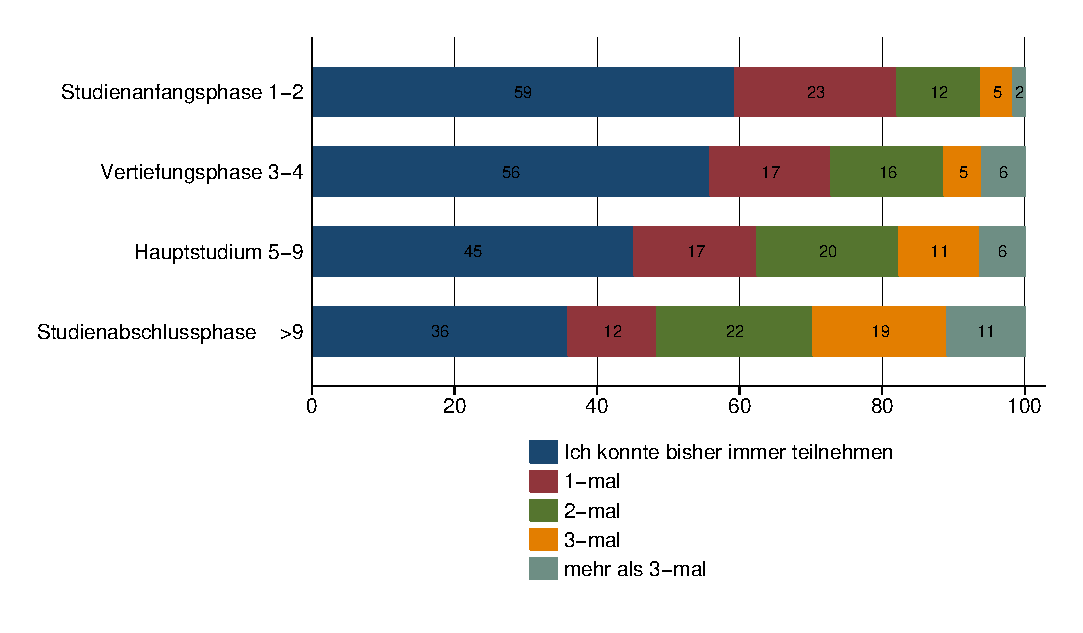
\includegraphics[
%  defaultresolution=72 !,
%  bmpsizefast=false
%]{image}
%\end{verbatim}
% \end{quote}
%
% \subsubsection{Hints}
%
% \begin{itemize}
% \item My version of \xfile{dvips.def} 1999/02/16 v3.0i defines
%       rules for the supported bitmap extensions, but does not
%       include them in the list of extensions that are tried
%       if the file name is not given with an extension.
%       In such a case, the list of extensions can be set
%       by \cs{DeclareGraphicsExtensions}, see \xpackage{grfguide}.
%       The following code just extends the list:
%       \begin{quote}
%\begin{verbatim}
%\makeatletter
%\g@addto@macro\Gin@extensions{,.bmp,.pcx,.msp}
%\makeatother
%\end{verbatim}
%       \end{quote}
% \item My version of \xfile{dvipdfm.def} 1998/11/24 vx.x misses
%       the graphics rule for PNG files. It can be added by:
%       \begin{quote}
%\begin{verbatim}
%\DeclareGraphicsRule{.png}{bmp}{.bb}{#1}
%\end{verbatim}
%       \end{quote}
%       See the previous issue to add the extension \xfile{.png} to the list
%       of extensions for package \xpackage{graphics}.
% \end{itemize}
%
% \subsubsection{Test program}
%
% There is a test program \xfile{bmpsize-test.tex}. Run it through
% \verb|latex|, \verb|pdflatex|, or \verb|pdftex|. Then given
% image files are inspected and the result is printed.
%
% \subsubsection{Interface for programmers}
%
% The macro names of the parsers are \verb|\bmpsize@read@|\meta{type}.
% Example: \cs{bmpsize@read@jpg} in case of JPEG.
%
% A parser sets the switch \cs{ifbmpsize@ok} to true, if it
% could successfully parse the image file.
% The width and height are returnd in \cs{bmpsize@width} and
% \cs{bmpsize@height}. If information about density is available,
% it is used to calculate width and height of the image, otherwise
% the values given by option \xoption{defaultresolution} is used.
% \xoption{resolution} overwrites the values in the image file.
%
% \subsection{Improved bitmap inclusion}
%
% Some drivers for package \xpackage{graphics} define the graphics
% type \xoption{bmp} for bitmap images. The code in the standard
% drivers for \xoption{dvips}, \xoption{dvipdfm}, and \xoption{dvipdfmx}
% is very basic and misses essential features of the
% package \xpackage{graphicx}. Therefore the code for bitmap
% inclusion is automatically rewritten by this package to add
% the following features:
% \begin{itemize}
% \item Support for \xoption{viewport} and \xoption{trim}.
% \item Support for \xoption{clip}.
% \item In case of \xoption{dvipdfm} and \xoption{dvipdfmx} the
%       bitmap images are reused and not included again if they
%       are used more than once.
% \end{itemize}
% However, there is a difference between \xoption{dvipdfm} and
% \xoption{dvipdfmx}, especially if images are reused. In the
% former case the reused box has width and height of 1bp, in the
% latter case its natural width. Thus the correct driver option must be given.
% \xoption{dvipdfm} and \xoption{dvipdfmx} are not equivalent.
%
% Older versions of \xoption{dvipdfmx} uses a size of 1in. However I do
% want to distinguish between versions of the same program. Therefore the
% support of these older versions has stopped with version 1.6 of this package.
% Use version dvipdfmx-20090708 or newer (some few versions before will
% probably also work, but I don't want to investigate this further).
%
% \StopEventually{
% }
%
% \section{Implementation}
%
% \subsection{Basic package \xpackage{bmpsize-base}}
%
%    Identification.
%    \begin{macrocode}
%<*base>
\ProvidesPackage{bmpsize-base}%
  [2009/09/04 v1.6 Basic part of bmpsize (HO)]%
%    \end{macrocode}
%    Modules of package \xpackage{fp} are used for calculations.
%    \begin{macrocode}
\RequirePackage{fp-basic}
\RequirePackage{fp-snap}
%    \end{macrocode}
%    Package \xpackage{fp} uses nested \cs{loop} structures.
%    That breaks with the plain-\TeX\ version of \cs{loop}.
%    Therefore we use the \LaTeX\ variant.
%    \begin{macro}{\@bmpsize@plain@loop}
%    \begin{macrocode}
\long\def\@bmpsize@plain@loop#1\repeat{%
  \def\iterate{%
    #1\relax
    \expandafter\iterate\fi
  }%
  \iterate
  \let\iterate\relax
}
%    \end{macrocode}
%    \end{macro}
%    \begin{macrocode}
\RequirePackage{pdftexcmds}[2007/11/11]
%    \end{macrocode}
%    \begin{macrocode}
\newif\ifbmpsize@ok
\let\@bmpsize@ok\bmpsize@oktrue

\newif\if@bmpsize@bigendian
\newif\if@bmpsize@absnum
\newif\if@bmpsize@user@resolution
\newif\if@bmpsize@fast
\@bmpsize@fasttrue

\def\@bmpsize@init{%
  \let\@bmpsize@org@plain@loop\loop
  \let\loop\@bmpsize@plain@loop
  \bmpsize@okfalse
  \@bmpsize@bigendiantrue
  \@bmpsize@absnumfalse
  \let\bmpsize@pixelwidth\relax
  \let\bmpsize@pixelheight\relax
  \let\bmpsize@pixelx\relax
  \let\bmpsize@pixely\relax
  \let\bmpsize@unit\relax
  \let\bmpsize@pixelxdenom\relax
  \let\bmpsize@pixelydenom\relax
  \let\bmpsize@orientation\relax
}

\def\@bmpsize@stop#1\@nil{}

\def\@bmpsize@loop#1{%
  #1%
  \@bmpsize@loop{#1}%
}
\def\@bmpsize@break#1\@bmpsize@loop#2{}

\def\@bmpsize@size#1#2#3{%
  \edef#3{\pdf@filesize{#1}}%
  \ifx#3\@empty
    \expandafter\@bmpsize@stop
  \fi
  \ifnum#3<#2\relax
    \expandafter\@bmpsize@stop
  \fi
}

\def\@bmpsize@read#1#2#3{%
  \edef\@bmpsize@buf{\pdf@filedump{#3}{#2}{#1}}%
  \edef\@bmpsize@temp{%
    \noexpand\@bmpsize@check@byte{#2}\@bmpsize@buf{}{}\noexpand\\%
  }%
  \@bmpsize@temp
}
\def\@bmpsize@fillbuf#1{%
  \ifx\@bmpsize@buf\@empty
    \expandafter\@firstofone
  \else
    \expandafter\@gobble
  \fi
  {%
    \edef\@bmpsize@buf{%
      \pdf@filedump{\bmpsize@offset}{\bmpsize@fillbuflength}{#1}%
    }%
    \ifx\@bmpsize@buf\@empty
      \expandafter\@bmpsize@stop
    \fi
    \edef\bmpsize@offset{\the\numexpr\bmpsize@offset+\bmpsize@fillbuflength}%
  }%
}
\def\bmpsize@fillbuflength{10}

\def\@bmpsize@append#1#2#3{%
  \edef#1{#2#3}%
}
\def\@bmpsize@pushback#1{%
  \edef\@bmpsize@buf{#1\@bmpsize@buf}%
}

\def\@bmpsize@iswhite#1{%
  \ifnum\pdf@strcmp{#1}{09}=\z@
  \else
    \ifnum\pdf@strcmp{#1}{0A}=\z@
    \else
      \ifnum\pdf@strcmp{#1}{0D}=\z@
      \else
        \ifnum\pdf@strcmp{#1}{20}=\z@
        \else
          1%
        \fi
      \fi
    \fi
  \fi
  \space
}
\def\@bmpsize@isdigit#1{%
  \ifnum\pdf@strcmp{#1}{30}<\z@
    1%
  \else
    \ifnum\pdf@strcmp{#1}{39}>\z@
      1%
    \fi
  \fi
  \space
}

\def\@bmpsize@check@byte#1#2#3{%
  \ifnum#1<\@ne
    \csname fi\endcsname
    \@bmpsize@cleanup@end
  \else
    \csname fi\endcsname
  \ifx!#2#3!%
    \csname fi\endcsname
    \@bmpsize@stop
  \else
    \csname fi\endcsname
    \expandafter\@bmpsize@check@byte\expandafter{\the\numexpr#1-1}%
}
\def\@bmpsize@cleanup@end#1\\{}

\def\@bmpsize@swap@maybe#1{%
  \if@bmpsize@bigendian
  \else
    \edef#1{\expandafter\@bmpsize@@swap#1\@empty\@empty\@empty\@empty}%
  \fi
}
\def\@bmpsize@@swap#1#2#3#4#5#6#7#8{%
  #7#8#5#6#3#4#1#2%
}

\def\@bmpsize@skip@one{%
  \edef\@bmpsize@buf{\expandafter\@gobbletwo\@bmpsize@buf}%
}
\def\@bmpsize@skip@two{%
  \edef\@bmpsize@buf{\expandafter\@gobblefour\@bmpsize@buf}%
}
\def\@bmpsize@skip@four{%
  \edef\@bmpsize@buf{%
    \expandafter\expandafter\expandafter\@gobblefour\expandafter
    \@gobblefour\@bmpsize@buf
  }%
}

\def\@bmpsize@grab#1#2{%
  \edef#1{\noexpand\@bmpsize@grab@byte#2=\@bmpsize@buf\noexpand\\}%
  \edef#1{#1}%
}
\def\@bmpsize@grab@byte#1=#2#3{%
  #2#3%
  \ifnum#1>\@ne
    \expandafter\@bmpsize@grab@byte\the\numexpr#1-1\expandafter=%
  \else
    \expandafter\@bmpsize@cleanup@end
  \fi
}

\def\@bmpsize@abs@maybe#1{%
  \let\@bmpsize@temp\relax
  \if@bmpsize@absnum
    \ifnum"\expandafter\@car#1\@nil>7 %
      \edef#1{\expandafter\@bmpsize@abs@byte#1\relax}%
      \ifnum\pdf@strcmp{#1}{7FFFFFFF}=\z@
        \let\@bmpsize@temp\@bmpsize@stop
      \else
        \def\@bmpsize@temp{\edef#1{\the\numexpr#1+1}}%
      \fi
    \fi
  \fi
}
\def\@bmpsize@abs@byte#1{%
  \ifx#1\relax
  \else
    \ifcase"0#1 %
      F\or E\or D\or C\or B\or A\or 9\or 8\or
      7\or 6\or 5\or 4\or 3\or 2\or 1\or 0%
    \fi
    \expandafter\@bmpsize@abs@byte
  \fi
}

\def\@bmpsize@num@one#1{%
  \@bmpsize@grab#11%
  \@bmpsize@abs@maybe#1%
  \edef#1{\number"#1}%
  \@bmpsize@temp
  \@bmpsize@skip@one
}
\def\@bmpsize@num@two#1{%
  \@bmpsize@grab#12%
  \@bmpsize@swap@maybe#1%
  \@bmpsize@abs@maybe#1%
  \edef#1{\number"#1}%
  \@bmpsize@temp
  \@bmpsize@skip@two
}
\def\@bmpsize@num@four#1{%
  \@bmpsize@grab#14%
  \@bmpsize@swap@maybe#1%
  \@bmpsize@abs@maybe#1%
  \ifnum\pdf@strcmp{#1}{7FFFFFFF}>\z@
    \expandafter\@bmpsize@stop
  \fi
  \edef#1{\number"#1}%
  \@bmpsize@temp
  \@bmpsize@skip@four
}

\def\@bmpsize@div#1#2#3{% #1 := #2/#3
  \FPdiv#1{#2}{#3}%
  \@bmpsize@beautify#1%
}
\def\@bmpsize@beautify#1{%
  \FPifint#1%
    \edef#1{\expandafter\@bmpsize@trunc#1.\@nil}%
  \else
    \edef#1{\expandafter\@bmpsize@cleanup@frac#1.\@nil}%
  \fi
}
\def\@bmpsize@trunc#1.#2\@nil{#1}
% #1 isn't an integer, thus we should have at least one
% necessary digit after the dot
\def\@bmpsize@cleanup@frac#1.#2#3.#4\@nil{%
  #1.#2%
  \ifx\\#3\\%
  \else
    \@bmpsize@cleanup@fracdigits#3000000000\@nil
  \fi
}
\def\@bmpsize@cleanup@fracdigits#1#2#3#4#5#6#7#8#9{%
  \ifcase#9 %
    \ifcase#8 %
      \ifcase#7 %
        \ifcase#6 %
          \ifcase#5 %
            \ifcase #4 %
              \ifcase #3 %
                \ifcase #2 %
                  \ifcase #1 %
                  \else
                    #1%
                  \fi
                \else
                  #1#2%
                \fi
              \else
                #1#2#3%
              \fi
            \else
              #1#2#3#4%
            \fi
          \else
            #1#2#3#4#5%
          \fi
        \else
          #1#2#3#4#5#6%
        \fi
      \else
        #1#2#3#4#5#6#7%
      \fi
    \else
      #1#2#3#4#5#6#7#8%
    \fi
  \else
    #1#2#3#4#5#6#7#8#9%
  \fi
  \@bmpsize@trunc.%
}

\def\@bmpsize@end{%
  \ifbmpsize@ok
    \ifx\bmpsize@pixelwidth\relax
      \bmpsize@okfalse
    \fi
    \ifx\bmpsize@pixelheight\relax
      \bmpsize@okfalse
    \fi
  \fi
  \ifbmpsize@ok
    \ifnum\bmpsize@pixelwidth>\z@
    \else
      \bmpsize@okfalse
    \fi
    \ifnum\bmpsize@pixelheight>\z@
    \else
      \bmpsize@okfalse
    \fi
  \fi
  \ifbmpsize@ok
    \ifcase 0%
      \ifx\bmpsize@pixelx\relax 1 \fi
      \ifx\bmpsize@pixely\relax 1 \fi
      \ifnum\bmpsize@pixelx>\z@\else 1 \fi
      \ifnum\bmpsize@pixely>\z@\else 1 \fi
      \ifx\bmpsize@pixelxdenom\relax
         \ifx\bmpsize@pixelydenom\relax\else 1 \fi
      \else
        \ifnum\bmpsize@pixelxdenom>\z@\else 1 \fi
      \fi
      \ifx\bmpsize@pixelydenom\relax
      \else
        \ifnum\bmpsize@pixelydenom>\z@\else 1 \fi
      \fi
    \else
      \let\bmpsize@pixelx\relax
      \let\bmpsize@pixely\relax
      \let\bmpsize@unit\relax
      \let\bmpsize@pixelxdenom\relax
      \let\bmpsize@pixelydenom\relax
    \fi
    \ifx\bmpsize@pixelxdenom\relax
    \else
      \@bmpsize@div\bmpsize@pixelx\bmpsize@pixelx\bmpsize@pixelxdenom
      \@bmpsize@div\bmpsize@pixely\bmpsize@pixely\bmpsize@pixelydenom
      \let\bmpsize@pixelxdenom\relax
      \let\bmpsize@pixelydenom\relax
    \fi
    \ifcase 0\ifx\bmpsize@unit\relax 1\fi
             \if@bmpsize@user@resolution 1\fi
             \relax
      \let\bmpsize@calc@unit\bmpsize@unit
      \let\bmpsize@calc@pixelx\bmpsize@pixelx
      \let\bmpsize@calc@pixely\bmpsize@pixely
    \else
      \let\bmpsize@calc@unit\bmpsize@unit@default
      \let\bmpsize@calc@pixelx\bmpsize@pixelx@default
      \let\bmpsize@calc@pixely\bmpsize@pixely@default
      \ifx\bmpsize@calc@pixely\Gin@exclamation
        \ifx\bmpsize@pixelx\relax
          \let\bmpsize@calc@pixely\bmpsize@calc@pixelx
        \else
          \FPdiv\bmpsize@calc@pixely\bmpsize@calc@pixelx\bmpsize@pixelx
          \FPmul\bmpsize@calc@pixely\bmpsize@calc@pixely\bmpsize@pixely
        \fi
      \else
        \ifx\bmpsize@calc@pixelx\Gin@exclamation
          \ifx\bmpsize@pixelx\relax
            \let\bmpsize@calc@pixelx\bmpsize@calc@pixely
          \else
            \FPdiv\bmpsize@calc@pixelx\bmpsize@calc@pixely\bmpsize@pixely
            \FPmul\bmpsize@calc@pixelx\bmpsize@calc@pixelx\bmpsize@pixelx
          \fi
        \fi
      \fi
    \fi
    \FPdiv\bmpsize@width\bmpsize@pixelwidth\bmpsize@calc@pixelx
    \FPdiv\bmpsize@height\bmpsize@pixelheight\bmpsize@calc@pixely
    % calculation of width and height in bp for package graphics
    % 1in = 72bp = 72.27pt, 72/72.27 = 8/8.03, 1pt = 65536sp
    \if@bmpsize@fast
      \edef\bmpsize@width{%
        \strip@pt\dimexpr.99626\dimexpr
        \bmpsize@width\dimexpr\bmpsize@calc@unit
      }%
      \edef\bmpsize@height{%
        \strip@pt\dimexpr.99626\dimexpr
        \bmpsize@height\dimexpr\bmpsize@calc@unit
      }%
    \else
      \edef\@bmpsize@temp{\number\dimexpr\bmpsize@calc@unit}%
      \ifnum\@bmpsize@temp>100000 %
        \FPmul\@bmpsize@temp\@bmpsize@temp{0.00001}%
        \def\@bmpsize@corr{100000}%
      \else
        \let\@bmpsize@corr\relax
      \fi
      \FPmul\bmpsize@width\bmpsize@width\@bmpsize@temp
      \FPmul\bmpsize@height\bmpsize@height\@bmpsize@temp
      \FPmul\bmpsize@width\bmpsize@width{8}%
      \FPmul\bmpsize@height\bmpsize@height{8}%
      \FPdiv\bmpsize@width\bmpsize@width{8.03}%
      \FPdiv\bmpsize@height\bmpsize@height{8.03}%
      \FPdiv\bmpsize@width\bmpsize@width{65536}%
      \FPdiv\bmpsize@height\bmpsize@height{65536}%
      \ifx\@bmpsize@corr\relax
      \else
        \FPmul\bmpsize@width\bmpsize@width\@bmpsize@corr
        \FPmul\bmpsize@height\bmpsize@height\@bmpsize@corr
      \fi
      \FPround\bmpsize@width\bmpsize@width{5}%
      \FPround\bmpsize@height\bmpsize@height{5}%
      \@bmpsize@beautify\bmpsize@width
      \@bmpsize@beautify\bmpsize@height
    \fi
  \fi
  \let\loop\@bmpsize@org@plain@loop
}
\def\bmpsize@unit@default{72.27pt}% more accurate than 1in
\def\bmpsize@pixelx@default{72}
\let\bmpsize@pixely@default\Gin@exclamation

\def\bmpsize@types{png,jpg,bmp,gif,tiff,pnm,pam,xpm,tga,pcx,msp,sgi}
%</base>
%    \end{macrocode}
%
% \subsection{Bitmap formats}
%
% \subsubsection{png}
%
%\iffalse
%<*ignore>
%\fi
%\begin{verbatim}
%begin png
%big-endian
%
%read 24 0
%grab 8        -> $temp
%check streq $temp [0x89 "PNG" 0x0D 0x0A 0x1A 0x0A]
%num 4         -> $length
%grab 4        -> $temp
%check streq $temp ["IHDR"]
%num 4         -> $pixelwidth
%num 4         -> $pixelheight
%ok
%assign numexpr(20 + $length) -> $offset
%loop
%  read 8 $offset
%  num 4       -> $length
%  grab 4      -> $temp
%  if streq $temp ["IDAT"]
%    stop
%  fi
%  if streq $temp ["pHYs"]
%    read 9 numexpr($offset + 8)
%    num 4     -> $pixelx
%    num 4     -> $pixely
%    grab 1     -> $temp
%    if numeq $temp 1
%      assign {100cm} -> $unit
%    fi
%    stop
%  fi
%  assign numexpr($offset + 12 + $length) -> $offset
%repeat
%end
%\end{verbatim}
%\iffalse
%</ignore>
%\fi
%    \begin{macro}{\bmpsize@read@png}
%    \begin{macrocode}
%<*base>
\def\bmpsize@read@png#1{%
  \@bmpsize@init
  \@bmpsize@bigendiantrue
  \@bmpsize@read{#1}{24}{0}%
  \@bmpsize@grab\bmpsize@temp{8}%
  \@bmpsize@skip@four
  \@bmpsize@skip@four
  \ifnum\pdf@strcmp{\bmpsize@temp}{89504E470D0A1A0A}=\z@
  \else
    \expandafter\@bmpsize@stop
  \fi
  \@bmpsize@num@four\bmpsize@length
  \@bmpsize@grab\bmpsize@temp{4}%
  \@bmpsize@skip@four
  \ifnum\pdf@strcmp{\bmpsize@temp}{49484452}=\z@
  \else
    \expandafter\@bmpsize@stop
  \fi
  \@bmpsize@num@four\bmpsize@pixelwidth
  \@bmpsize@num@four\bmpsize@pixelheight
  \@bmpsize@ok
  \edef\bmpsize@offset{\the\numexpr20+\bmpsize@length}%
  \@bmpsize@loop{%
    \@bmpsize@read{#1}{8}{\bmpsize@offset}%
    \@bmpsize@num@four\bmpsize@length
    \@bmpsize@grab\bmpsize@temp{4}%
    \@bmpsize@skip@four
    \ifnum\pdf@strcmp{\bmpsize@temp}{49444154}=\z@
      \expandafter\@firstofone
    \else
      \expandafter\@gobble
    \fi
    {%
      \@bmpsize@stop
    }%
    \ifnum\pdf@strcmp{\bmpsize@temp}{70485973}=\z@
      \expandafter\@firstofone
    \else
      \expandafter\@gobble
    \fi
    {%
      \@bmpsize@read{#1}{9}{\numexpr\bmpsize@offset+8\relax}%
      \@bmpsize@num@four\bmpsize@pixelx
      \@bmpsize@num@four\bmpsize@pixely
      \@bmpsize@grab\bmpsize@temp{1}%
      \@bmpsize@skip@one
      \ifnum\bmpsize@temp=1\relax
        \expandafter\@firstofone
      \else
        \expandafter\@gobble
      \fi
      {%
        \def\bmpsize@unit{100cm}%
      }%
      \@bmpsize@stop
    }%
    \edef\bmpsize@offset{\the\numexpr\bmpsize@offset+12+\bmpsize@length}%
  }%
  \@bmpsize@stop
  \@nil
  \@bmpsize@end
}%
%</base>
%    \end{macrocode}
%    \end{macro}
%
% \subsubsection{jpg}
%
%\iffalse
%<*ignore>
%\fi
%\begin{verbatim}
%begin jpg
%
%read 3 0
%grab 3      -> $temp % SOI and 0xFF
%check streq $temp [0xFF 0xD8 0xFF]
%assign {2} -> $offset
%assign {0} -> $exifdensity
%loop
%  read 4 $offset
%  grab 1    -> $temp
%  check streq $temp [0xFF]
%  num 1    -> $temp
%  if numeq $temp 0xDA % SOS
%    stop
%  fi
%  % look for JFIF APP0 segment
%  if numeq $temp 0xE0 % APP0
%    num 2       -> $length
%    if numeq $exifdensity 0
%      if numge $length 16 % a JFIF segment has 16 bytes at least
%        read 12 numexpr($offset + 4)
%        grab 5      -> $temp % identifier
%        if streq $temp ["JFIF" 0x0]
%          check numge $length 16
%          skip 2 % version
%          num 1       -> $temp % units
%          if numeq $temp 1
%            assign {72.27pt} -> $unit
%          else
%            if numeq $temp 2
%              assign {1cm} -> $unit
%            fi
%          fi
%          num 2    -> $pixelx
%          num 2    -> $pixely
%        fi
%      fi
%    fi
%  else
%    if numeq $temp 0xE1 % APP1
%      % look for Exif APP1 segment
%      num 2 -> $length
%      if numge $length 20 % identifier (6) + Tiff header (8) + first IFD (>=6)
%        read 20 numexpr($offset + 4)
%        grab 6 -> $temp
%        if streq $temp ["Exif" 0x0 0x0]
%          assign numexpr($offset + 10) -> $exifoffset
%          % read TIFF header
%          grab 2 -> $temp
%          if streq $temp ["II"]
%            little-endian
%          else
%            check streq $temp ["MM"]
%            % big-endian
%          fi
%          num 2 -> $temp
%          check numeq $temp 42
%          num 4 -> $temp % offset of first IFD
%          check numgt $temp 0
%          % read first IFD
%          assign numexpr($temp + $exifoffset) -> $off
%          read 2 $off
%          num 2 -> $entries
%          assign numexpr($off + 2) -> $off
%          loop
%            if numeq $entries 0
%              break
%            fi
%            assign numexpr($entries - 1) -> $entries
%            % entry format:
%            % 2 tag
%            % 2 field type
%            % 4 count
%            % 4 value/offset
%            read 12 $off
%            assign numexpr($off + 12) -> $off
%            num 2 -> $tag
%            if numeq $tag 296 % ResolutionUnit
%              skip 6 % type: 3 (short), count: 1
%              num 2 -> $temp
%              ifcase $temp
%              or % 1
%                clear $unit
%              or % 2
%                assign {72.27pt} -> $unit
%              or % 3
%                assign {1cm} -> $unit
%              else
%                clear $unit % unknown
%              fi
%              ifcase $temp
%              or % 1
%              or % 2
%                assign {1} -> $exifdensity
%              or % 3
%                assign {1} -> $exifdensity
%              else
%                assign $exifdensity -> $exifdensity
%              fi
%            fi
%            % 256 ImageWidth (use width of JPG part)
%            % 257 ImageHeight (use height of JPG part)
%            if numeq $tag 274 % Orientation
%              skip 6 % type: 3 (short), count: 1
%              num 2 -> $temp
%              if numge $temp 0 
%                if numle $temp 8
%                  assign $temp -> $orientation
%                fi
%              fi
%            fi
%            if numeq $tag 282 % XResolution
%              skip 6
%              num 4 -> $temp
%              read 8 numexpr($temp + $exifoffset)
%              num 4 -> $pixelx
%              num 4 -> $temp
%              if numeq $temp 1
%              else
%                assign numexpr($temp) -> $pixelxdenom
%                % div $pixelx $temp -> $pixelx
%              fi
%            fi
%            if numeq $tag 283 % YResolution
%              skip 6
%              num 4 -> $temp
%              read 8 numexpr($temp + $exifoffset)
%              num 4 -> $pixely
%              num 4 -> $temp
%              if numeq $temp 1
%              else
%                assign numexpr($temp) -> $pixelydenom
%                % div $pixely $temp -> $pixely
%              fi
%            fi
%          repeat
%          big-endian
%        fi
%      fi
%    else
%      assign numexpr($temp - 0xC0) -> $temp
%      ifcase $temp % SOF_0
%      or % SOF_1
%      or % SOF_2
%      or % SOF_3
%      or % DHT
%        assign {-1} -> $temp
%      or % SOF_5
%      or % SOF_6
%      or % SOF_7
%      or % JPG
%        assign {-1} -> $temp
%      or % SOF_9
%      or % SOF_10
%      or % SOF_11
%      or % DAC
%        assign {-1} -> $temp
%      or % SOF_13
%      or % SOF_14
%      or % SOF_15
%      else
%        assign {-1} -> $temp
%      fi
%      if numeq $temp -1
%      else
%        read 4 numexpr($offset + 5)
%        num 2  -> $pixelheight
%        num 2  -> $pixelwidth
%        if numeq $pixelheight 0
%          clear $pixelheight
%          stop
%        fi
%        ok
%        stop
%      fi
%      num 2 -> $length
%    fi
%  fi
%  assign numexpr($offset + $length + 2) -> $offset
%repeat
%end
%\end{verbatim}
%\iffalse
%</ignore>
%\fi
%    \begin{macro}{\bmpsize@read@jpg}
%    \begin{macrocode}
%<*base>
\def\bmpsize@read@jpg#1{%
  \@bmpsize@init
  \@bmpsize@read{#1}{3}{0}%
  \@bmpsize@grab\bmpsize@temp{3}%
  \@bmpsize@skip@two
  \@bmpsize@skip@one
  \ifnum\pdf@strcmp{\bmpsize@temp}{FFD8FF}=\z@
  \else
    \expandafter\@bmpsize@stop
  \fi
  \def\bmpsize@offset{2}%
  \def\bmpsize@exifdensity{0}%
  \@bmpsize@loop{%
    \@bmpsize@read{#1}{4}{\bmpsize@offset}%
    \@bmpsize@grab\bmpsize@temp{1}%
    \@bmpsize@skip@one
    \ifnum\pdf@strcmp{\bmpsize@temp}{FF}=\z@
    \else
      \expandafter\@bmpsize@stop
    \fi
    \@bmpsize@num@one\bmpsize@temp
    \ifnum\bmpsize@temp=218\relax
      \expandafter\@firstofone
    \else
      \expandafter\@gobble
    \fi
    {%
      \@bmpsize@stop
    }%
    \ifnum\bmpsize@temp=224\relax
      \expandafter\@firstoftwo
    \else
      \expandafter\@secondoftwo
    \fi
    {%
      \@bmpsize@num@two\bmpsize@length
      \ifnum\bmpsize@exifdensity=0\relax
        \expandafter\@firstofone
      \else
        \expandafter\@gobble
      \fi
      {%
        \unless\ifnum\bmpsize@length<16\relax
          \expandafter\@firstofone
        \else
          \expandafter\@gobble
        \fi
        {%
          \@bmpsize@read{#1}{12}{\numexpr\bmpsize@offset+4\relax}%
          \@bmpsize@grab\bmpsize@temp{5}%
          \@bmpsize@skip@four
          \@bmpsize@skip@one
          \ifnum\pdf@strcmp{\bmpsize@temp}{4A46494600}=\z@
            \expandafter\@firstofone
          \else
            \expandafter\@gobble
          \fi
          {%
            \ifnum\bmpsize@length<16\relax
              \expandafter\@bmpsize@stop
            \fi
            \@bmpsize@skip@two
            \@bmpsize@num@one\bmpsize@temp
            \ifnum\bmpsize@temp=1\relax
              \expandafter\@firstoftwo
            \else
              \expandafter\@secondoftwo
            \fi
            {%
              \def\bmpsize@unit{72.27pt}%
            }{%
              \ifnum\bmpsize@temp=2\relax
                \expandafter\@firstofone
              \else
                \expandafter\@gobble
              \fi
              {%
                \def\bmpsize@unit{1cm}%
              }%
            }%
            \@bmpsize@num@two\bmpsize@pixelx
            \@bmpsize@num@two\bmpsize@pixely
          }%
        }%
      }%
    }{%
      \ifnum\bmpsize@temp=225\relax
        \expandafter\@firstoftwo
      \else
        \expandafter\@secondoftwo
      \fi
      {%
        \@bmpsize@num@two\bmpsize@length
        \unless\ifnum\bmpsize@length<20\relax
          \expandafter\@firstofone
        \else
          \expandafter\@gobble
        \fi
        {%
          \@bmpsize@read{#1}{20}{\numexpr\bmpsize@offset+4\relax}%
          \@bmpsize@grab\bmpsize@temp{6}%
          \@bmpsize@skip@four
          \@bmpsize@skip@two
          \ifnum\pdf@strcmp{\bmpsize@temp}{457869660000}=\z@
            \expandafter\@firstofone
          \else
            \expandafter\@gobble
          \fi
          {%
            \edef\bmpsize@exifoffset{\the\numexpr\bmpsize@offset+10}%
            \@bmpsize@grab\bmpsize@temp{2}%
            \@bmpsize@skip@two
            \ifnum\pdf@strcmp{\bmpsize@temp}{4949}=\z@
              \expandafter\@firstoftwo
            \else
              \expandafter\@secondoftwo
            \fi
            {%
              \@bmpsize@bigendianfalse
            }{%
              \ifnum\pdf@strcmp{\bmpsize@temp}{4D4D}=\z@
              \else
                \expandafter\@bmpsize@stop
              \fi
            }%
            \@bmpsize@num@two\bmpsize@temp
            \ifnum\bmpsize@temp=42\relax
            \else
              \expandafter\@bmpsize@stop
            \fi
            \@bmpsize@num@four\bmpsize@temp
            \ifnum\bmpsize@temp>0\relax
            \else
              \expandafter\@bmpsize@stop
            \fi
            \edef\bmpsize@off{\the\numexpr\bmpsize@temp+\bmpsize@exifoffset}%
            \@bmpsize@read{#1}{2}{\bmpsize@off}%
            \@bmpsize@num@two\bmpsize@entries
            \edef\bmpsize@off{\the\numexpr\bmpsize@off+2}%
            \@bmpsize@loop{%
              \ifnum\bmpsize@entries=0\relax
                \expandafter\@firstofone
              \else
                \expandafter\@gobble
              \fi
              {%
                \@bmpsize@break
              }%
              \edef\bmpsize@entries{\the\numexpr\bmpsize@entries-1}%
              \@bmpsize@read{#1}{12}{\bmpsize@off}%
              \edef\bmpsize@off{\the\numexpr\bmpsize@off+12}%
              \@bmpsize@num@two\bmpsize@tag
              \ifnum\bmpsize@tag=296\relax
                \expandafter\@firstofone
              \else
                \expandafter\@gobble
              \fi
              {%
                \@bmpsize@skip@four
                \@bmpsize@skip@two
                \@bmpsize@num@two\bmpsize@temp
                \ifcase\bmpsize@temp\relax
                \or
                  \let\bmpsize@unit\relax
                \or
                  \def\bmpsize@unit{72.27pt}%
                \or
                  \def\bmpsize@unit{1cm}%
                \else
                  \let\bmpsize@unit\relax
                \fi
                \ifcase\bmpsize@temp\relax
                \or
                \or
                  \def\bmpsize@exifdensity{1}%
                \or
                  \def\bmpsize@exifdensity{1}%
                \else
                  \let\bmpsize@exifdensity\bmpsize@exifdensity
                \fi
              }%
              \ifnum\bmpsize@tag=274\relax
                \expandafter\@firstofone
              \else
                \expandafter\@gobble
              \fi
              {%
                \@bmpsize@skip@four
                \@bmpsize@skip@two
                \@bmpsize@num@two\bmpsize@temp
                \unless\ifnum\bmpsize@temp<0\relax
                  \expandafter\@firstofone
                \else
                  \expandafter\@gobble
                \fi
                {%
                  \unless\ifnum\bmpsize@temp>8\relax
                    \expandafter\@firstofone
                  \else
                    \expandafter\@gobble
                  \fi
                  {%
                    \let\bmpsize@orientation\bmpsize@temp
                  }%
                }%
              }%
              \ifnum\bmpsize@tag=282\relax
                \expandafter\@firstofone
              \else
                \expandafter\@gobble
              \fi
              {%
                \@bmpsize@skip@four
                \@bmpsize@skip@two
                \@bmpsize@num@four\bmpsize@temp
                \@bmpsize@read{#1}{8}{\numexpr\bmpsize@temp+\bmpsize@exifoffset\relax}%
                \@bmpsize@num@four\bmpsize@pixelx
                \@bmpsize@num@four\bmpsize@temp
                \ifnum\bmpsize@temp=1\relax
                  \expandafter\@gobble
                \else
                  \expandafter\@firstofone
                \fi
                {%
                  \edef\bmpsize@pixelxdenom{\the\numexpr\bmpsize@temp}%
                }%
              }%
              \ifnum\bmpsize@tag=283\relax
                \expandafter\@firstofone
              \else
                \expandafter\@gobble
              \fi
              {%
                \@bmpsize@skip@four
                \@bmpsize@skip@two
                \@bmpsize@num@four\bmpsize@temp
                \@bmpsize@read{#1}{8}{\numexpr\bmpsize@temp+\bmpsize@exifoffset\relax}%
                \@bmpsize@num@four\bmpsize@pixely
                \@bmpsize@num@four\bmpsize@temp
                \ifnum\bmpsize@temp=1\relax
                  \expandafter\@gobble
                \else
                  \expandafter\@firstofone
                \fi
                {%
                  \edef\bmpsize@pixelydenom{\the\numexpr\bmpsize@temp}%
                }%
              }%
            }%
            \@bmpsize@bigendiantrue
          }%
        }%
      }{%
        \edef\bmpsize@temp{\the\numexpr\bmpsize@temp-192}%
        \ifcase\bmpsize@temp\relax
        \or
        \or
        \or
        \or
          \def\bmpsize@temp{-1}%
        \or
        \or
        \or
        \or
          \def\bmpsize@temp{-1}%
        \or
        \or
        \or
        \or
          \def\bmpsize@temp{-1}%
        \or
        \or
        \or
        \else
          \def\bmpsize@temp{-1}%
        \fi
        \ifnum\bmpsize@temp=-1\relax
          \expandafter\@gobble
        \else
          \expandafter\@firstofone
        \fi
        {%
          \@bmpsize@read{#1}{4}{\numexpr\bmpsize@offset+5\relax}%
          \@bmpsize@num@two\bmpsize@pixelheight
          \@bmpsize@num@two\bmpsize@pixelwidth
          \ifnum\bmpsize@pixelheight=0\relax
            \expandafter\@firstofone
          \else
            \expandafter\@gobble
          \fi
          {%
            \let\bmpsize@pixelheight\relax
            \@bmpsize@stop
          }%
          \@bmpsize@ok
          \@bmpsize@stop
        }%
        \@bmpsize@num@two\bmpsize@length
      }%
    }%
    \edef\bmpsize@offset{\the\numexpr\bmpsize@offset+\bmpsize@length+2}%
  }%
  \@bmpsize@stop
  \@nil
  \@bmpsize@end
}%
%</base>
%    \end{macrocode}
%    \end{macro}
%
% \subsubsection{bmp}
%
%\iffalse
%<*ignore>
%\fi
%\begin{verbatim}
%begin bmp
%little-endian
%
%read 26 0
%grab 2 -> $temp
%check streq $temp ["BM"]
%skip 12
%% header size is 4 bytes in V3+, unknown for V1, V2,
%% known header sizes fit in 2 bytes
%num 2   -> $temp
%if numeq $temp 12 % V1
%  skip 2
%  num 2 -> $pixelwidth
%  num 2 -> $pixelheight
%  % no resolution entries
%  ok
%  stop
%fi
%if numeq $temp 64 % V2
%  skip 2
%  num 2 -> $pixelwidth
%  num 2 -> $pixelheight
%  % missing specification for resolution
%  ok
%  stop
%fi
%% V3, V4, V5
%skip 2
%num 4 -> $pixelwidth
%absnum 4 -> $pixelheight
%ok
%read 8 38
%num 4 -> $pixelx
%num 4 -> $pixely
%assign {100cm} -> $unit
%end
%\end{verbatim}
%\iffalse
%</ignore>
%\fi
%    \begin{macro}{\bmpsize@read@bmp}
%    \begin{macrocode}
%<*base>
\def\bmpsize@read@bmp#1{%
  \@bmpsize@init
  \@bmpsize@bigendianfalse
  \@bmpsize@read{#1}{26}{0}%
  \@bmpsize@grab\bmpsize@temp{2}%
  \@bmpsize@skip@two
  \ifnum\pdf@strcmp{\bmpsize@temp}{424D}=\z@
  \else
    \expandafter\@bmpsize@stop
  \fi
  \@bmpsize@skip@four
  \@bmpsize@skip@four
  \@bmpsize@skip@four
  \@bmpsize@num@two\bmpsize@temp
  \ifnum\bmpsize@temp=12\relax
    \expandafter\@firstofone
  \else
    \expandafter\@gobble
  \fi
  {%
    \@bmpsize@skip@two
    \@bmpsize@num@two\bmpsize@pixelwidth
    \@bmpsize@num@two\bmpsize@pixelheight
    \@bmpsize@ok
    \@bmpsize@stop
  }%
  \ifnum\bmpsize@temp=64\relax
    \expandafter\@firstofone
  \else
    \expandafter\@gobble
  \fi
  {%
    \@bmpsize@skip@two
    \@bmpsize@num@two\bmpsize@pixelwidth
    \@bmpsize@num@two\bmpsize@pixelheight
    \@bmpsize@ok
    \@bmpsize@stop
  }%
  \@bmpsize@skip@two
  \@bmpsize@num@four\bmpsize@pixelwidth
  \@bmpsize@absnumtrue
  \@bmpsize@num@four\bmpsize@pixelheight
  \@bmpsize@absnumfalse
  \@bmpsize@ok
  \@bmpsize@read{#1}{8}{38}%
  \@bmpsize@num@four\bmpsize@pixelx
  \@bmpsize@num@four\bmpsize@pixely
  \def\bmpsize@unit{100cm}%
  \@bmpsize@stop
  \@nil
  \@bmpsize@end
}%
%</base>
%    \end{macrocode}
%    \end{macro}
%
% \subsubsection{gif}
%
%\iffalse
%<*ignore>
%\fi
%\begin{verbatim}
%begin gif
%little-endian
%
%% Header
%read 13 0
%grab 3      -> $temp
%check streq $temp ["GIF"]
%skip 3      % version
%
%% Logical Screen Descriptor
%num 2       -> $pixelwidth
%num 2       -> $pixelheight
%skip 2
%num 1       -> $temp % Pixel Aspect Ratio
%if numeq $temp 0
%else
%  assign numexpr($temp + 15) -> $pixelx
%  assign {64}     -> $pixely
%fi
%ok
%end
%\end{verbatim}
%\iffalse
%</ignore>
%\fi
%    \begin{macro}{\bmpsize@read@gif}
%    \begin{macrocode}
%<*base>
\def\bmpsize@read@gif#1{%
  \@bmpsize@init
  \@bmpsize@bigendianfalse
  \@bmpsize@read{#1}{13}{0}%
  \@bmpsize@grab\bmpsize@temp{3}%
  \@bmpsize@skip@two
  \@bmpsize@skip@one
  \ifnum\pdf@strcmp{\bmpsize@temp}{474946}=\z@
  \else
    \expandafter\@bmpsize@stop
  \fi
  \@bmpsize@skip@two
  \@bmpsize@skip@one
  \@bmpsize@num@two\bmpsize@pixelwidth
  \@bmpsize@num@two\bmpsize@pixelheight
  \@bmpsize@skip@two
  \@bmpsize@num@one\bmpsize@temp
  \ifnum\bmpsize@temp=0\relax
    \expandafter\@gobble
  \else
    \expandafter\@firstofone
  \fi
  {%
    \edef\bmpsize@pixelx{\the\numexpr\bmpsize@temp+15}%
    \def\bmpsize@pixely{64}%
  }%
  \@bmpsize@ok
  \@bmpsize@stop
  \@nil
  \@bmpsize@end
}%
%</base>
%    \end{macrocode}
%    \end{macro}
%
% \subsubsection{tiff}
%
%\iffalse
%<*ignore>
%\fi
%\begin{verbatim}
%begin tiff
%% defaults
%assign {72.27pt} -> $unit
%
%% Image File Header
%read 8 0
%grab 2 -> $temp
%if streq $temp ["II"]
%  little-endian
%else
%  check streq $temp ["MM"]
%  big-endian
%fi
%num 2 -> $temp
%check numeq $temp 42
%num 4 -> $offset % first IFD (Image File Directory)
%
%% First IFD
%read 2 $offset
%assign numexpr($offset + 2) -> $offset
%num 2 -> $entries
%ok % must rely on checks at the end
%loop
%  if numeq $entries 0
%    stop
%  fi
%  assign numexpr($entries - 1) -> $entries
%  % entry format:
%  % 2 tag
%  % 2 field type
%  % 4 count
%  % 4 value/offset
%  read 12 $offset
%  assign numexpr($offset + 12) -> $offset
%  num 2 -> $tag % tag
%  if numeq $temp 296 % ResolutionUnit
%    skip 6 % type: 3 (short), count: 1
%    num 2 -> $temp
%    ifcase $temp
%    or % 1
%      clear $unit
%    or % 2
%      assign {72.27pt} -> $unit
%    or % 3
%      assign {1cm} -> $unit
%    else
%      clear $unit
%    fi
%  fi
%  if numeq $tag 256 % ImageWidth
%    skip 6
%    num 4 -> $pixelwidth
%  fi
%  if numeq $tag 257 % ImageLength
%    skip 6
%    num 4 -> $pixelheight
%  fi
%  if numeq $tag 282 % XResolution
%    skip 6
%    num 4 -> $temp
%    read 8 $temp
%    num 4 -> $pixelx
%    num 4 -> $temp
%    if numeq $temp 1
%    else
%      assign numexpr($temp) -> $pixelxdenom
%      % div $pixelx $temp -> $pixelx
%    fi
%  fi
%  if numeq $tag 283 % YResolution
%    skip 6
%    num 4 -> $temp
%    read 8 $temp
%    num 4 -> $pixely
%    num 4 -> $temp
%    if numeq $temp 1
%    else
%      assign numexpr($temp) -> $pixelydenom
%      % div $pixely $temp -> $pixely
%    fi
%  fi
%repeat
%end
%\end{verbatim}
%\iffalse
%</ignore>
%\fi
%    \begin{macro}{\bmpsize@read@tiff}
%    \begin{macrocode}
%<*base>
\def\bmpsize@read@tiff#1{%
  \@bmpsize@init
  \def\bmpsize@unit{72.27pt}%
  \@bmpsize@read{#1}{8}{0}%
  \@bmpsize@grab\bmpsize@temp{2}%
  \@bmpsize@skip@two
  \ifnum\pdf@strcmp{\bmpsize@temp}{4949}=\z@
    \expandafter\@firstoftwo
  \else
    \expandafter\@secondoftwo
  \fi
  {%
    \@bmpsize@bigendianfalse
  }{%
    \ifnum\pdf@strcmp{\bmpsize@temp}{4D4D}=\z@
    \else
      \expandafter\@bmpsize@stop
    \fi
    \@bmpsize@bigendiantrue
  }%
  \@bmpsize@num@two\bmpsize@temp
  \ifnum\bmpsize@temp=42\relax
  \else
    \expandafter\@bmpsize@stop
  \fi
  \@bmpsize@num@four\bmpsize@offset
  \@bmpsize@read{#1}{2}{\bmpsize@offset}%
  \edef\bmpsize@offset{\the\numexpr\bmpsize@offset+2}%
  \@bmpsize@num@two\bmpsize@entries
  \@bmpsize@ok
  \@bmpsize@loop{%
    \ifnum\bmpsize@entries=0\relax
      \expandafter\@firstofone
    \else
      \expandafter\@gobble
    \fi
    {%
      \@bmpsize@stop
    }%
    \edef\bmpsize@entries{\the\numexpr\bmpsize@entries-1}%
    \@bmpsize@read{#1}{12}{\bmpsize@offset}%
    \edef\bmpsize@offset{\the\numexpr\bmpsize@offset+12}%
    \@bmpsize@num@two\bmpsize@tag
    \ifnum\bmpsize@temp=296\relax
      \expandafter\@firstofone
    \else
      \expandafter\@gobble
    \fi
    {%
      \@bmpsize@skip@four
      \@bmpsize@skip@two
      \@bmpsize@num@two\bmpsize@temp
      \ifcase\bmpsize@temp\relax
      \or
        \let\bmpsize@unit\relax
      \or
        \def\bmpsize@unit{72.27pt}%
      \or
        \def\bmpsize@unit{1cm}%
      \else
        \let\bmpsize@unit\relax
      \fi
    }%
    \ifnum\bmpsize@tag=256\relax
      \expandafter\@firstofone
    \else
      \expandafter\@gobble
    \fi
    {%
      \@bmpsize@skip@four
      \@bmpsize@skip@two
      \@bmpsize@num@four\bmpsize@pixelwidth
    }%
    \ifnum\bmpsize@tag=257\relax
      \expandafter\@firstofone
    \else
      \expandafter\@gobble
    \fi
    {%
      \@bmpsize@skip@four
      \@bmpsize@skip@two
      \@bmpsize@num@four\bmpsize@pixelheight
    }%
    \ifnum\bmpsize@tag=282\relax
      \expandafter\@firstofone
    \else
      \expandafter\@gobble
    \fi
    {%
      \@bmpsize@skip@four
      \@bmpsize@skip@two
      \@bmpsize@num@four\bmpsize@temp
      \@bmpsize@read{#1}{8}{\bmpsize@temp}%
      \@bmpsize@num@four\bmpsize@pixelx
      \@bmpsize@num@four\bmpsize@temp
      \ifnum\bmpsize@temp=1\relax
        \expandafter\@gobble
      \else
        \expandafter\@firstofone
      \fi
      {%
        \edef\bmpsize@pixelxdenom{\the\numexpr\bmpsize@temp}%
      }%
    }%
    \ifnum\bmpsize@tag=283\relax
      \expandafter\@firstofone
    \else
      \expandafter\@gobble
    \fi
    {%
      \@bmpsize@skip@four
      \@bmpsize@skip@two
      \@bmpsize@num@four\bmpsize@temp
      \@bmpsize@read{#1}{8}{\bmpsize@temp}%
      \@bmpsize@num@four\bmpsize@pixely
      \@bmpsize@num@four\bmpsize@temp
      \ifnum\bmpsize@temp=1\relax
        \expandafter\@gobble
      \else
        \expandafter\@firstofone
      \fi
      {%
        \edef\bmpsize@pixelydenom{\the\numexpr\bmpsize@temp}%
      }%
    }%
  }%
  \@bmpsize@stop
  \@nil
  \@bmpsize@end
}%
%</base>
%    \end{macrocode}
%    \end{macro}
%
% \subsubsection{pnm}
%
%\iffalse
%<*ignore>
%\fi
%\begin{verbatim}
%begin pnm
%assign {0} -> $offset
%read 3 $offset
%assign {3} -> $offset
%grab 1 -> $temp
%check streq $temp ["P"]
%grab 1 -> $temp
%check strge $temp ["1"]
%check strle $temp ["6"]
%% ensure one white space
%grab 1 -> $temp
%if iswhite $temp
%else
%  stop
%fi
%loop
%  % skip white space
%  fillbuf
%  grab 1 -> $temp
%  if iswhite $temp
%  else
%    if streq $temp ["#"]
%      % ignore comments
%      loop
%        fillbuf
%        grab 1 -> $temp
%        if streq $temp [0x0A]
%          break
%        else
%          if streq $temp [0x0D]
%            break
%          fi
%        fi
%      repeat
%    else
%      pushback $temp
%      break
%    fi
%  fi
%repeat
%assign {} -> $tempnum
%loop
%  fillbuf
%  grab 1 -> $temp
%  if isdigit $temp
%    append $tempnum $temp -> $tempnum
%  else
%    if iswhite $temp
%      break
%    else
%      stop
%    fi
%  fi
%repeat
%assign unescapehex($tempnum) -> $pixelwidth
%loop
%  fillbuf
%  grab 1 -> $temp
%  if iswhite $temp
%  else
%    pushback $temp
%    break
%  fi
%repeat
%assign {} -> $tempnum
%loop
%  fillbuf
%  grab 1 -> $temp
%  if isdigit $temp
%    append $tempnum $temp -> $tempnum
%  else
%    if iswhite $temp
%      break
%    else
%      stop
%    fi
%  fi
%repeat
%assign unescapehex($tempnum) -> $pixelheight
%ok
%end
%\end{verbatim}
%\iffalse
%</ignore>
%\fi
%    \begin{macro}{\bmpsize@read@pnm}
%    \begin{macrocode}
%<*base>
\def\bmpsize@read@pnm#1{%
  \@bmpsize@init
  \def\bmpsize@offset{0}%
  \@bmpsize@read{#1}{3}{\bmpsize@offset}%
  \def\bmpsize@offset{3}%
  \@bmpsize@grab\bmpsize@temp{1}%
  \@bmpsize@skip@one
  \ifnum\pdf@strcmp{\bmpsize@temp}{50}=\z@
  \else
    \expandafter\@bmpsize@stop
  \fi
  \@bmpsize@grab\bmpsize@temp{1}%
  \@bmpsize@skip@one
  \ifnum\pdf@strcmp{\bmpsize@temp}{31}<\z@
    \expandafter\@bmpsize@stop
  \fi
  \ifnum\pdf@strcmp{\bmpsize@temp}{36}>\z@
    \expandafter\@bmpsize@stop
  \fi
  \@bmpsize@grab\bmpsize@temp{1}%
  \@bmpsize@skip@one
  \ifcase 0\@bmpsize@iswhite\bmpsize@temp
    \expandafter\@gobble
  \else
    \expandafter\@firstofone
  \fi
  {%
    \@bmpsize@stop
  }%
  \@bmpsize@loop{%
    \@bmpsize@fillbuf{#1}%
    \@bmpsize@grab\bmpsize@temp{1}%
    \@bmpsize@skip@one
    \ifcase 0\@bmpsize@iswhite\bmpsize@temp
      \expandafter\@gobble
    \else
      \expandafter\@firstofone
    \fi
    {%
      \ifnum\pdf@strcmp{\bmpsize@temp}{23}=\z@
        \expandafter\@firstoftwo
      \else
        \expandafter\@secondoftwo
      \fi
      {%
        \@bmpsize@loop{%
          \@bmpsize@fillbuf{#1}%
          \@bmpsize@grab\bmpsize@temp{1}%
          \@bmpsize@skip@one
          \ifnum\pdf@strcmp{\bmpsize@temp}{0A}=\z@
            \expandafter\@firstoftwo
          \else
            \expandafter\@secondoftwo
          \fi
          {%
            \@bmpsize@break
          }{%
            \ifnum\pdf@strcmp{\bmpsize@temp}{0D}=\z@
              \expandafter\@firstofone
            \else
              \expandafter\@gobble
            \fi
            {%
              \@bmpsize@break
            }%
          }%
        }%
      }{%
        \@bmpsize@pushback\bmpsize@temp
        \@bmpsize@break
      }%
    }%
  }%
  \def\bmpsize@tempnum{}%
  \@bmpsize@loop{%
    \@bmpsize@fillbuf{#1}%
    \@bmpsize@grab\bmpsize@temp{1}%
    \@bmpsize@skip@one
    \ifcase 0\@bmpsize@isdigit\bmpsize@temp
      \expandafter\@firstoftwo
    \else
      \expandafter\@secondoftwo
    \fi
    {%
      \@bmpsize@append\bmpsize@tempnum\bmpsize@tempnum\bmpsize@temp
    }{%
      \ifcase 0\@bmpsize@iswhite\bmpsize@temp
        \expandafter\@firstoftwo
      \else
        \expandafter\@secondoftwo
      \fi
      {%
        \@bmpsize@break
      }{%
        \@bmpsize@stop
      }%
    }%
  }%
  \edef\bmpsize@pixelwidth{\pdf@unescapehex{\bmpsize@tempnum}}%
  \@bmpsize@loop{%
    \@bmpsize@fillbuf{#1}%
    \@bmpsize@grab\bmpsize@temp{1}%
    \@bmpsize@skip@one
    \ifcase 0\@bmpsize@iswhite\bmpsize@temp
      \expandafter\@gobble
    \else
      \expandafter\@firstofone
    \fi
    {%
      \@bmpsize@pushback\bmpsize@temp
      \@bmpsize@break
    }%
  }%
  \def\bmpsize@tempnum{}%
  \@bmpsize@loop{%
    \@bmpsize@fillbuf{#1}%
    \@bmpsize@grab\bmpsize@temp{1}%
    \@bmpsize@skip@one
    \ifcase 0\@bmpsize@isdigit\bmpsize@temp
      \expandafter\@firstoftwo
    \else
      \expandafter\@secondoftwo
    \fi
    {%
      \@bmpsize@append\bmpsize@tempnum\bmpsize@tempnum\bmpsize@temp
    }{%
      \ifcase 0\@bmpsize@iswhite\bmpsize@temp
        \expandafter\@firstoftwo
      \else
        \expandafter\@secondoftwo
      \fi
      {%
        \@bmpsize@break
      }{%
        \@bmpsize@stop
      }%
    }%
  }%
  \edef\bmpsize@pixelheight{\pdf@unescapehex{\bmpsize@tempnum}}%
  \@bmpsize@ok
  \@bmpsize@stop
  \@nil
  \@bmpsize@end
}%
%</base>
%    \end{macrocode}
%    \end{macro}
%
% \subsubsection{pam}
%
%\iffalse
%<*ignore>
%\fi
%\begin{verbatim}
%begin pam
%read 3 0
%assign {3} -> $offset
%assign $offset -> $off
%grab 3 -> $temp
%check streq $temp ["P7" 0x0A]
%loop
%  fillbuf
%  grab 1 -> $temp
%  if iswhite $temp
%    % ignore white space
%    assign numexpr($off + 1) -> $off
%  else
%    if streq $temp ["#"]
%      % ignore comment line
%      assign numexpr($off + 1) -> $off
%      loop
%        fillbuf
%        grab 1 -> $temp
%        assign numexpr($off + 1) -> $off
%        if streq $temp [0x0A]
%          break
%        fi
%      repeat
%    else
%      read 6 $off
%      assign numexpr($off + 6) -> $offset
%      grab 5 -> $head
%      if streq $head ["WIDTH"]
%        assign numexpr($off + 5) -> $off
%        % skip white space
%        loop
%          fillbuf
%          grab 1 -> $temp
%          if iswhite $temp
%            assign numexpr($off + 1) -> $off
%          else
%            if isdigit $temp
%              assign numexpr($off + 1) -> $off
%              break
%            else
%              % error
%              stop
%            fi
%          fi
%        repeat
%        % read number
%        assign $temp -> $tempnum
%        loop
%          fillbuf
%          grab 1 -> $temp
%          if isdigit $temp
%            assign numexpr($off + 1) -> $off
%            append $tempnum $temp -> $tempnum
%          else
%            pushback $temp
%            break
%          fi
%        repeat
%        % skip to end of line
%        loop
%          fillbuf
%          grab 1 -> $temp
%          assign numexpr($off + 1) -> $off
%          if streq $temp [0x0A]
%            break
%          fi
%        repeat
%        assign unescapehex($tempnum) -> $pixelwidth
%      else
%        grab 1 -> $temp
%        append $head $temp -> $head
%        if streq $head ["ENDHDR"]
%          % last header line
%          ok
%          stop
%        else
%          if streq $head ["HEIGHT"]
%            assign numexpr($off + 6) -> $off
%            % skip white space
%            loop
%              fillbuf
%              grab 1 -> $temp
%              if iswhite $temp
%                assign numexpr($off + 1) -> $off
%              else
%                if isdigit $temp
%                  assign numexpr($off + 1) -> $off
%                  break
%                else
%                  % error
%                  stop
%                fi
%              fi
%            repeat
%            % read number
%            assign $temp -> $tempnum
%            loop
%              fillbuf
%              grab 1 -> $temp
%              if isdigit $temp
%                assign numexpr($off + 1) -> $off
%                append $tempnum $temp -> $tempnum
%              else
%                pushback $temp
%                break
%              fi
%            repeat
%            % skip to end of line
%            loop
%              fillbuf
%              grab 1 -> $temp
%              assign numexpr($off + 1) -> $off
%              if streq $temp [0x0A]
%                break
%              fi
%            repeat
%            assign unescapehex($tempnum) -> $pixelheight
%          else
%            % ignore unknown header line
%            pushback $head
%            loop
%              fillbuf
%              grab 1 -> $temp
%              assign numexpr($off + 1) -> $off
%              if streq $temp [0x0A]
%                break
%              fi
%            repeat
%          fi
%        fi
%      fi
%    fi
%  fi
%repeat
%end
%\end{verbatim}
%\iffalse
%</ignore>
%\fi
%    \begin{macro}{\bmpsize@read@pam}
%    \begin{macrocode}
%<*base>
\def\bmpsize@read@pam#1{%
  \@bmpsize@init
  \@bmpsize@read{#1}{3}{0}%
  \def\bmpsize@offset{3}%
  \let\bmpsize@off\bmpsize@offset
  \@bmpsize@grab\bmpsize@temp{3}%
  \@bmpsize@skip@two
  \@bmpsize@skip@one
  \ifnum\pdf@strcmp{\bmpsize@temp}{50370A}=\z@
  \else
    \expandafter\@bmpsize@stop
  \fi
  \@bmpsize@loop{%
    \@bmpsize@fillbuf{#1}%
    \@bmpsize@grab\bmpsize@temp{1}%
    \@bmpsize@skip@one
    \ifcase 0\@bmpsize@iswhite\bmpsize@temp
      \expandafter\@firstoftwo
    \else
      \expandafter\@secondoftwo
    \fi
    {%
      \edef\bmpsize@off{\the\numexpr\bmpsize@off+1}%
    }{%
      \ifnum\pdf@strcmp{\bmpsize@temp}{23}=\z@
        \expandafter\@firstoftwo
      \else
        \expandafter\@secondoftwo
      \fi
      {%
        \edef\bmpsize@off{\the\numexpr\bmpsize@off+1}%
        \@bmpsize@loop{%
          \@bmpsize@fillbuf{#1}%
          \@bmpsize@grab\bmpsize@temp{1}%
          \@bmpsize@skip@one
          \edef\bmpsize@off{\the\numexpr\bmpsize@off+1}%
          \ifnum\pdf@strcmp{\bmpsize@temp}{0A}=\z@
            \expandafter\@firstofone
          \else
            \expandafter\@gobble
          \fi
          {%
            \@bmpsize@break
          }%
        }%
      }{%
        \@bmpsize@read{#1}{6}{\bmpsize@off}%
        \edef\bmpsize@offset{\the\numexpr\bmpsize@off+6}%
        \@bmpsize@grab\bmpsize@head{5}%
        \@bmpsize@skip@four
        \@bmpsize@skip@one
        \ifnum\pdf@strcmp{\bmpsize@head}{5749445448}=\z@
          \expandafter\@firstoftwo
        \else
          \expandafter\@secondoftwo
        \fi
        {%
          \edef\bmpsize@off{\the\numexpr\bmpsize@off+5}%
          \@bmpsize@loop{%
            \@bmpsize@fillbuf{#1}%
            \@bmpsize@grab\bmpsize@temp{1}%
            \@bmpsize@skip@one
            \ifcase 0\@bmpsize@iswhite\bmpsize@temp
              \expandafter\@firstoftwo
            \else
              \expandafter\@secondoftwo
            \fi
            {%
              \edef\bmpsize@off{\the\numexpr\bmpsize@off+1}%
            }{%
              \ifcase 0\@bmpsize@isdigit\bmpsize@temp
                \expandafter\@firstoftwo
              \else
                \expandafter\@secondoftwo
              \fi
              {%
                \edef\bmpsize@off{\the\numexpr\bmpsize@off+1}%
                \@bmpsize@break
              }{%
                \@bmpsize@stop
              }%
            }%
          }%
          \let\bmpsize@tempnum\bmpsize@temp
          \@bmpsize@loop{%
            \@bmpsize@fillbuf{#1}%
            \@bmpsize@grab\bmpsize@temp{1}%
            \@bmpsize@skip@one
            \ifcase 0\@bmpsize@isdigit\bmpsize@temp
              \expandafter\@firstoftwo
            \else
              \expandafter\@secondoftwo
            \fi
            {%
              \edef\bmpsize@off{\the\numexpr\bmpsize@off+1}%
              \@bmpsize@append\bmpsize@tempnum\bmpsize@tempnum\bmpsize@temp
            }{%
              \@bmpsize@pushback\bmpsize@temp
              \@bmpsize@break
            }%
          }%
          \@bmpsize@loop{%
            \@bmpsize@fillbuf{#1}%
            \@bmpsize@grab\bmpsize@temp{1}%
            \@bmpsize@skip@one
            \edef\bmpsize@off{\the\numexpr\bmpsize@off+1}%
            \ifnum\pdf@strcmp{\bmpsize@temp}{0A}=\z@
              \expandafter\@firstofone
            \else
              \expandafter\@gobble
            \fi
            {%
              \@bmpsize@break
            }%
          }%
          \edef\bmpsize@pixelwidth{\pdf@unescapehex{\bmpsize@tempnum}}%
        }{%
          \@bmpsize@grab\bmpsize@temp{1}%
          \@bmpsize@skip@one
          \@bmpsize@append\bmpsize@head\bmpsize@head\bmpsize@temp
          \ifnum\pdf@strcmp{\bmpsize@head}{454E44484452}=\z@
            \expandafter\@firstoftwo
          \else
            \expandafter\@secondoftwo
          \fi
          {%
            \@bmpsize@ok
            \@bmpsize@stop
          }{%
            \ifnum\pdf@strcmp{\bmpsize@head}{484549474854}=\z@
              \expandafter\@firstoftwo
            \else
              \expandafter\@secondoftwo
            \fi
            {%
              \edef\bmpsize@off{\the\numexpr\bmpsize@off+6}%
              \@bmpsize@loop{%
                \@bmpsize@fillbuf{#1}%
                \@bmpsize@grab\bmpsize@temp{1}%
                \@bmpsize@skip@one
                \ifcase 0\@bmpsize@iswhite\bmpsize@temp
                  \expandafter\@firstoftwo
                \else
                  \expandafter\@secondoftwo
                \fi
                {%
                  \edef\bmpsize@off{\the\numexpr\bmpsize@off+1}%
                }{%
                  \ifcase 0\@bmpsize@isdigit\bmpsize@temp
                    \expandafter\@firstoftwo
                  \else
                    \expandafter\@secondoftwo
                  \fi
                  {%
                    \edef\bmpsize@off{\the\numexpr\bmpsize@off+1}%
                    \@bmpsize@break
                  }{%
                    \@bmpsize@stop
                  }%
                }%
              }%
              \let\bmpsize@tempnum\bmpsize@temp
              \@bmpsize@loop{%
                \@bmpsize@fillbuf{#1}%
                \@bmpsize@grab\bmpsize@temp{1}%
                \@bmpsize@skip@one
                \ifcase 0\@bmpsize@isdigit\bmpsize@temp
                  \expandafter\@firstoftwo
                \else
                  \expandafter\@secondoftwo
                \fi
                {%
                  \edef\bmpsize@off{\the\numexpr\bmpsize@off+1}%
                  \@bmpsize@append\bmpsize@tempnum\bmpsize@tempnum\bmpsize@temp
                }{%
                  \@bmpsize@pushback\bmpsize@temp
                  \@bmpsize@break
                }%
              }%
              \@bmpsize@loop{%
                \@bmpsize@fillbuf{#1}%
                \@bmpsize@grab\bmpsize@temp{1}%
                \@bmpsize@skip@one
                \edef\bmpsize@off{\the\numexpr\bmpsize@off+1}%
                \ifnum\pdf@strcmp{\bmpsize@temp}{0A}=\z@
                  \expandafter\@firstofone
                \else
                  \expandafter\@gobble
                \fi
                {%
                  \@bmpsize@break
                }%
              }%
              \edef\bmpsize@pixelheight{\pdf@unescapehex{\bmpsize@tempnum}}%
            }{%
              \@bmpsize@pushback\bmpsize@head
              \@bmpsize@loop{%
                \@bmpsize@fillbuf{#1}%
                \@bmpsize@grab\bmpsize@temp{1}%
                \@bmpsize@skip@one
                \edef\bmpsize@off{\the\numexpr\bmpsize@off+1}%
                \ifnum\pdf@strcmp{\bmpsize@temp}{0A}=\z@
                  \expandafter\@firstofone
                \else
                  \expandafter\@gobble
                \fi
                {%
                  \@bmpsize@break
                }%
              }%
            }%
          }%
        }%
      }%
    }%
  }%
  \@bmpsize@stop
  \@nil
  \@bmpsize@end
}%
%</base>
%    \end{macrocode}
%    \end{macro}
%
% \subsubsection{xpm}
%
%\iffalse
%<*ignore>
%\fi
%\begin{verbatim}
%begin xpm
%read 9 0
%grab 9 -> $temp
%assign {9} -> $offset
%check streq $temp ["/* XPM */"]
%loop
%  fillbuf
%  grab 1 -> $temp
%  if streq $temp [0x22] % "
%    break
%  fi
%  if streq $temp ["/"]
%    fillbuf
%    grab 1 -> $temp
%    if streq $temp ["*"]
%      % look for end of C comment
%      loop
%        fillbuf
%        grab 1 -> $temp
%        if streq $temp ["*"]
%          loop
%            fillbuf
%            grab 1 -> $temp
%            if streq $temp ["/"]
%              break
%            fi
%            if streq $temp ["*"]
%            else
%              break
%            fi
%          repeat
%          if streq $temp ["/"]
%            break
%          fi
%        fi
%      repeat
%    fi
%  fi
%repeat
%% width
%assign {} -> $tempnum
%loop
%  fillbuf
%  grab 1 -> $temp
%  if iswhite $temp
%  else
%    if isdigit $temp
%      append $tempnum $temp -> $tempnum
%      break
%    else
%      stop
%    fi
%  fi
%repeat
%loop
%  fillbuf
%  grab 1 -> $temp
%  if isdigit $temp
%    append $tempnum $temp -> $tempnum
%  else
%    if iswhite $temp
%      break
%    else
%      stop
%    fi
%  fi
%repeat
%assign unescapehex($tempnum) -> $pixelwidth
%% height
%assign {} -> $tempnum
%loop
%  fillbuf
%  grab 1 -> $temp
%  if iswhite $temp
%  else
%    if isdigit $temp
%      append $tempnum $temp -> $tempnum
%      break
%    else
%      stop
%    fi
%  fi
%repeat
%loop
%  fillbuf
%  grab 1 -> $temp
%  if isdigit $temp
%    append $tempnum $temp -> $tempnum
%  else
%    if iswhite $temp
%      break
%    else
%      stop
%    fi
%  fi
%repeat
%assign unescapehex($tempnum) -> $pixelheight
%ok
%end
%\end{verbatim}
%\iffalse
%</ignore>
%\fi
%    \begin{macro}{\bmpsize@read@xpm}
%    \begin{macrocode}
%<*base>
\def\bmpsize@read@xpm#1{%
  \@bmpsize@init
  \@bmpsize@read{#1}{9}{0}%
  \@bmpsize@grab\bmpsize@temp{9}%
  \@bmpsize@skip@four
  \@bmpsize@skip@four
  \@bmpsize@skip@one
  \def\bmpsize@offset{9}%
  \ifnum\pdf@strcmp{\bmpsize@temp}{2F2A2058504D202A2F}=\z@
  \else
    \expandafter\@bmpsize@stop
  \fi
  \@bmpsize@loop{%
    \@bmpsize@fillbuf{#1}%
    \@bmpsize@grab\bmpsize@temp{1}%
    \@bmpsize@skip@one
    \ifnum\pdf@strcmp{\bmpsize@temp}{22}=\z@
      \expandafter\@firstofone
    \else
      \expandafter\@gobble
    \fi
    {%
      \@bmpsize@break
    }%
    \ifnum\pdf@strcmp{\bmpsize@temp}{2F}=\z@
      \expandafter\@firstofone
    \else
      \expandafter\@gobble
    \fi
    {%
      \@bmpsize@fillbuf{#1}%
      \@bmpsize@grab\bmpsize@temp{1}%
      \@bmpsize@skip@one
      \ifnum\pdf@strcmp{\bmpsize@temp}{2A}=\z@
        \expandafter\@firstofone
      \else
        \expandafter\@gobble
      \fi
      {%
        \@bmpsize@loop{%
          \@bmpsize@fillbuf{#1}%
          \@bmpsize@grab\bmpsize@temp{1}%
          \@bmpsize@skip@one
          \ifnum\pdf@strcmp{\bmpsize@temp}{2A}=\z@
            \expandafter\@firstofone
          \else
            \expandafter\@gobble
          \fi
          {%
            \@bmpsize@loop{%
              \@bmpsize@fillbuf{#1}%
              \@bmpsize@grab\bmpsize@temp{1}%
              \@bmpsize@skip@one
              \ifnum\pdf@strcmp{\bmpsize@temp}{2F}=\z@
                \expandafter\@firstofone
              \else
                \expandafter\@gobble
              \fi
              {%
                \@bmpsize@break
              }%
              \ifnum\pdf@strcmp{\bmpsize@temp}{2A}=\z@
                \expandafter\@gobble
              \else
                \expandafter\@firstofone
              \fi
              {%
                \@bmpsize@break
              }%
            }%
            \ifnum\pdf@strcmp{\bmpsize@temp}{2F}=\z@
              \expandafter\@firstofone
            \else
              \expandafter\@gobble
            \fi
            {%
              \@bmpsize@break
            }%
          }%
        }%
      }%
    }%
  }%
  \def\bmpsize@tempnum{}%
  \@bmpsize@loop{%
    \@bmpsize@fillbuf{#1}%
    \@bmpsize@grab\bmpsize@temp{1}%
    \@bmpsize@skip@one
    \ifcase 0\@bmpsize@iswhite\bmpsize@temp
      \expandafter\@gobble
    \else
      \expandafter\@firstofone
    \fi
    {%
      \ifcase 0\@bmpsize@isdigit\bmpsize@temp
        \expandafter\@firstoftwo
      \else
        \expandafter\@secondoftwo
      \fi
      {%
        \@bmpsize@append\bmpsize@tempnum\bmpsize@tempnum\bmpsize@temp
        \@bmpsize@break
      }{%
        \@bmpsize@stop
      }%
    }%
  }%
  \@bmpsize@loop{%
    \@bmpsize@fillbuf{#1}%
    \@bmpsize@grab\bmpsize@temp{1}%
    \@bmpsize@skip@one
    \ifcase 0\@bmpsize@isdigit\bmpsize@temp
      \expandafter\@firstoftwo
    \else
      \expandafter\@secondoftwo
    \fi
    {%
      \@bmpsize@append\bmpsize@tempnum\bmpsize@tempnum\bmpsize@temp
    }{%
      \ifcase 0\@bmpsize@iswhite\bmpsize@temp
        \expandafter\@firstoftwo
      \else
        \expandafter\@secondoftwo
      \fi
      {%
        \@bmpsize@break
      }{%
        \@bmpsize@stop
      }%
    }%
  }%
  \edef\bmpsize@pixelwidth{\pdf@unescapehex{\bmpsize@tempnum}}%
  \def\bmpsize@tempnum{}%
  \@bmpsize@loop{%
    \@bmpsize@fillbuf{#1}%
    \@bmpsize@grab\bmpsize@temp{1}%
    \@bmpsize@skip@one
    \ifcase 0\@bmpsize@iswhite\bmpsize@temp
      \expandafter\@gobble
    \else
      \expandafter\@firstofone
    \fi
    {%
      \ifcase 0\@bmpsize@isdigit\bmpsize@temp
        \expandafter\@firstoftwo
      \else
        \expandafter\@secondoftwo
      \fi
      {%
        \@bmpsize@append\bmpsize@tempnum\bmpsize@tempnum\bmpsize@temp
        \@bmpsize@break
      }{%
        \@bmpsize@stop
      }%
    }%
  }%
  \@bmpsize@loop{%
    \@bmpsize@fillbuf{#1}%
    \@bmpsize@grab\bmpsize@temp{1}%
    \@bmpsize@skip@one
    \ifcase 0\@bmpsize@isdigit\bmpsize@temp
      \expandafter\@firstoftwo
    \else
      \expandafter\@secondoftwo
    \fi
    {%
      \@bmpsize@append\bmpsize@tempnum\bmpsize@tempnum\bmpsize@temp
    }{%
      \ifcase 0\@bmpsize@iswhite\bmpsize@temp
        \expandafter\@firstoftwo
      \else
        \expandafter\@secondoftwo
      \fi
      {%
        \@bmpsize@break
      }{%
        \@bmpsize@stop
      }%
    }%
  }%
  \edef\bmpsize@pixelheight{\pdf@unescapehex{\bmpsize@tempnum}}%
  \@bmpsize@ok
  \@bmpsize@stop
  \@nil
  \@bmpsize@end
}%
%</base>
%    \end{macrocode}
%    \end{macro}
%
% \subsubsection{tga}
%
%\iffalse
%<*ignore>
%\fi
%\begin{verbatim}
%begin tga
%little-endian
%                              % id length (1 byte)
%read 16 1
%grab 1 -> $temp               % color map type (1 byte), values: 0, 1
%if streq $temp [0x00]
%else
%  if streq $temp [0x01]
%  else
%    stop
%  fi
%fi
%skip 10                       % image type (1 byte)
%                              % color map specification (5 bytes)
%                              % x origin (2 bytes)
%                              % y origin (2 bytes)
%num 2 -> $pixelwidth          % image width
%num 2 -> $pixelheight         % image height
%ok
%% TGA File Footer
%size 26 -> $temp
%read 26 numexpr($temp - 26)
%num 4 -> $offset              % the extension area offset
%skip 4                        % the developer directory offset
%grab 18 -> $temp              % the signature, ".", 0x00
%if streq $temp ["TRUEVISION-XFILE." 0x00]
%else
%  stop
%fi
%if numeq $offset 0
%  stop                        % no extension area
%fi
%read 4 numexpr($offset + 474) % pixel aspect ratio (4 bytes)
%num 2 -> $pixelx              % pixel ratio numerator (pixel width)
%num 2 -> $pixely              % pixel ratio denominator (pixel height)
%if numeq $pixely 0            % no pixel aspect ratio
%  clear $pixelx
%  clear $pixely
%fi
%end
%\end{verbatim}
%\iffalse
%</ignore>
%\fi
%    \begin{macro}{\bmpsize@read@tga}
%    \begin{macrocode}
%<*base>
\def\bmpsize@read@tga#1{%
  \@bmpsize@init
  \@bmpsize@bigendianfalse
  \@bmpsize@read{#1}{16}{1}%
  \@bmpsize@grab\bmpsize@temp{1}%
  \@bmpsize@skip@one
  \ifnum\pdf@strcmp{\bmpsize@temp}{00}=\z@
    \expandafter\@gobble
  \else
    \expandafter\@firstofone
  \fi
  {%
    \ifnum\pdf@strcmp{\bmpsize@temp}{01}=\z@
      \expandafter\@gobble
    \else
      \expandafter\@firstofone
    \fi
    {%
      \@bmpsize@stop
    }%
  }%
  \@bmpsize@skip@four
  \@bmpsize@skip@four
  \@bmpsize@skip@two
  \@bmpsize@num@two\bmpsize@pixelwidth
  \@bmpsize@num@two\bmpsize@pixelheight
  \@bmpsize@ok
  \@bmpsize@size{#1}{26}\bmpsize@temp  \@bmpsize@read{#1}{26}{\numexpr\bmpsize@temp-26\relax}%
  \@bmpsize@num@four\bmpsize@offset
  \@bmpsize@skip@four
  \@bmpsize@grab\bmpsize@temp{18}%
  \@bmpsize@skip@four
  \@bmpsize@skip@four
  \@bmpsize@skip@four
  \@bmpsize@skip@four
  \@bmpsize@skip@two
  \ifnum\pdf@strcmp{\bmpsize@temp}{54525545564953494F4E2D5846494C452E00}=\z@
    \expandafter\@gobble
  \else
    \expandafter\@firstofone
  \fi
  {%
    \@bmpsize@stop
  }%
  \ifnum\bmpsize@offset=0\relax
    \expandafter\@firstofone
  \else
    \expandafter\@gobble
  \fi
  {%
    \@bmpsize@stop
  }%
  \@bmpsize@read{#1}{4}{\numexpr\bmpsize@offset+474\relax}%
  \@bmpsize@num@two\bmpsize@pixelx
  \@bmpsize@num@two\bmpsize@pixely
  \ifnum\bmpsize@pixely=0\relax
    \expandafter\@firstofone
  \else
    \expandafter\@gobble
  \fi
  {%
    \let\bmpsize@pixelx\relax
    \let\bmpsize@pixely\relax
  }%
  \@bmpsize@stop
  \@nil
  \@bmpsize@end
}%
%</base>
%    \end{macrocode}
%    \end{macro}
%
% \subsubsection{pcx}
%
%\iffalse
%<*ignore>
%\fi
%\begin{verbatim}
%begin pcx
%little-endian
%read 16 0
%grab 1 -> $temp             % manufacturer
%check streq $temp [0x0A]
%skip 1                      % version
%num 1 -> $temp              % encoding
%check numeq $temp 1
%skip 1                      % bits per pixel
%num 2 -> $pixelwidth        % x_min
%num 2 -> $pixelheight       % y_min
%num 2 -> $temp              % x_max
%assign numexpr($temp - $pixelwidth + 1) -> $pixelwidth
%num 2 -> $temp              % y_max
%assign numexpr($temp - $pixelheight + 1) -> $pixelheight
%check numgt $pixelwidth 0
%check numgt $pixelheight 0
%ok
%num 2 -> $pixelx            % horizontal resolution in DPI
%num 2 -> $pixely            % vertical resolution in DPI
%assign {72.27pt} -> $unit
%end
%\end{verbatim}
%\iffalse
%</ignore>
%\fi
%    \begin{macro}{\bmpsize@read@pcx}
%    \begin{macrocode}
%<*base>
\def\bmpsize@read@pcx#1{%
  \@bmpsize@init
  \@bmpsize@bigendianfalse
  \@bmpsize@read{#1}{16}{0}%
  \@bmpsize@grab\bmpsize@temp{1}%
  \@bmpsize@skip@one
  \ifnum\pdf@strcmp{\bmpsize@temp}{0A}=\z@
  \else
    \expandafter\@bmpsize@stop
  \fi
  \@bmpsize@skip@one
  \@bmpsize@num@one\bmpsize@temp
  \ifnum\bmpsize@temp=1\relax
  \else
    \expandafter\@bmpsize@stop
  \fi
  \@bmpsize@skip@one
  \@bmpsize@num@two\bmpsize@pixelwidth
  \@bmpsize@num@two\bmpsize@pixelheight
  \@bmpsize@num@two\bmpsize@temp
  \edef\bmpsize@pixelwidth{\the\numexpr\bmpsize@temp-\bmpsize@pixelwidth+1}%
  \@bmpsize@num@two\bmpsize@temp
  \edef\bmpsize@pixelheight{\the\numexpr\bmpsize@temp-\bmpsize@pixelheight+1}%
  \ifnum\bmpsize@pixelwidth>0\relax
  \else
    \expandafter\@bmpsize@stop
  \fi
  \ifnum\bmpsize@pixelheight>0\relax
  \else
    \expandafter\@bmpsize@stop
  \fi
  \@bmpsize@ok
  \@bmpsize@num@two\bmpsize@pixelx
  \@bmpsize@num@two\bmpsize@pixely
  \def\bmpsize@unit{72.27pt}%
  \@bmpsize@stop
  \@nil
  \@bmpsize@end
}%
%</base>
%    \end{macrocode}
%    \end{macro}
%
% \subsubsection{msp}
%
%\iffalse
%<*ignore>
%\fi
%\begin{verbatim}
%begin msp
%little-endian
%
%read 16 0
%
%% header 4
%grab 4 -> $temp
%if streq $temp ["DanM"]
%else
%  check streq $temp ["LinS"]
%fi
%num 2 -> $pixelwidth
%num 2 -> $pixelheight
%ok
%num 2 -> $pixelx % x_asp
%num 2 -> $pixely % y_asp
%assign {72.27pt} -> $unit % guessing
%if numeq $pixelx 0
%  num 2 -> $pixelx % x_asp_prn
%  num 2 -> $pixely % y_asp_prn
%fi
%% num 2 % width_prn
%% num 2 % height_prn
%end
%\end{verbatim}
%\iffalse
%</ignore>
%\fi
%    \begin{macro}{\bmpsize@read@msp}
%    \begin{macrocode}
%<*base>
\def\bmpsize@read@msp#1{%
  \@bmpsize@init
  \@bmpsize@bigendianfalse
  \@bmpsize@read{#1}{16}{0}%
  \@bmpsize@grab\bmpsize@temp{4}%
  \@bmpsize@skip@four
  \ifnum\pdf@strcmp{\bmpsize@temp}{44616E4D}=\z@
    \expandafter\@gobble
  \else
    \expandafter\@firstofone
  \fi
  {%
    \ifnum\pdf@strcmp{\bmpsize@temp}{4C696E53}=\z@
    \else
      \expandafter\@bmpsize@stop
    \fi
  }%
  \@bmpsize@num@two\bmpsize@pixelwidth
  \@bmpsize@num@two\bmpsize@pixelheight
  \@bmpsize@ok
  \@bmpsize@num@two\bmpsize@pixelx
  \@bmpsize@num@two\bmpsize@pixely
  \def\bmpsize@unit{72.27pt}%
  \ifnum\bmpsize@pixelx=0\relax
    \expandafter\@firstofone
  \else
    \expandafter\@gobble
  \fi
  {%
    \@bmpsize@num@two\bmpsize@pixelx
    \@bmpsize@num@two\bmpsize@pixely
  }%
  \@bmpsize@stop
  \@nil
  \@bmpsize@end
}%
%</base>
%    \end{macrocode}
%    \end{macro}
%
% \subsubsection{sgi}
%
%\iffalse
%<*ignore>
%\fi
%\begin{verbatim}
%begin sgi
%big-endian
%read 10 0
%grab 2 -> $temp
%check streq $temp [0x01 0xDA] % magic: 474 decimal
%grab 1 -> $temp               % storage: 0 or 1
%check numge $temp 0
%check numle $temp 1
%skip 2                        % bpc, dimension
%num 2 -> $pixelwidth
%num 2 -> $pixelheight
%ok
%end
%\end{verbatim}
%\iffalse
%</ignore>
%\fi
%    \begin{macro}{\bmpsize@read@sgi}
%    \begin{macrocode}
%<*base>
\def\bmpsize@read@sgi#1{%
  \@bmpsize@init
  \@bmpsize@bigendiantrue
  \@bmpsize@read{#1}{10}{0}%
  \@bmpsize@grab\bmpsize@temp{2}%
  \@bmpsize@skip@two
  \ifnum\pdf@strcmp{\bmpsize@temp}{01DA}=\z@
  \else
    \expandafter\@bmpsize@stop
  \fi
  \@bmpsize@grab\bmpsize@temp{1}%
  \@bmpsize@skip@one
  \ifnum\bmpsize@temp<0\relax
    \expandafter\@bmpsize@stop
  \fi
  \ifnum\bmpsize@temp>1\relax
    \expandafter\@bmpsize@stop
  \fi
  \@bmpsize@skip@two
  \@bmpsize@num@two\bmpsize@pixelwidth
  \@bmpsize@num@two\bmpsize@pixelheight
  \@bmpsize@ok
  \@bmpsize@stop
  \@nil
  \@bmpsize@end
}%
%</base>
%    \end{macrocode}
%    \end{macro}
%
% \subsection{Package \xpackage{bmpsize}}
%
%    \begin{macrocode}
%<*package>
\ProvidesPackage{bmpsize}%
  [2009/09/04 v1.6 Extract size/resolution from bitmap files (HO)]%
\RequirePackage{ifpdf}
\ifpdf
  \PackageInfo{bmpsize}{Superseded by pdfTeX in PDF mode}%
  \expandafter\endinput
\fi
\RequirePackage{pdftexcmds}[2007/11/11]
\begingroup\expandafter\expandafter\expandafter\endgroup
\expandafter\ifx\csname pdf@filedump\endcsname\relax
  \PackageError{bmpsize}{%
    You need pdfTeX 1.30.0 or newer%
  }{Package loading is aborted.}%
  \expandafter\endinput
\fi

\RequirePackage{infwarerr}[2007/09/09]
\RequirePackage{graphics}
%    \end{macrocode}
%    In case of \plainTeX\ options are not executed
%    and \cs{KV@err} and \cs{KV@errx} are undefined.
%    \begin{macrocode}
\RequirePackage{keyval}\relax
\expandafter\ifx\csname KV@errx\endcsname\relax
  \def\KV@errx#1{%
    \@PackageError{keyval}{#1}\@ehc
  }%
\fi
\expandafter\ifx\csname KV@err\endcsname\relax
  \let\KV@err\KV@errx
\fi
%    \end{macrocode}
%    \begin{macrocode}
\RequirePackage{bmpsize-base}

\InputIfFileExists{bmpsize-\Gin@driver}{}{}

\define@key{Gin}{bmpsizefast}[true]{%
  \expandafter\ifx\csname if#1\expandafter\endcsname\csname iftrue\endcsname
    \@bmpsize@fasttrue
  \else
    \@bmpsize@fastfalse
  \fi
}
\define@key{Gin}{resolutionunit}{%
  \def\bmpsize@unit@default{#1}%
}
\begingroup
  \def\x#1{\endgroup
    \define@key{Gin}{resolution}{%
      \@bmpsize@read@resolution\@bmpsize@user@resolutiontrue##1#1#1\@nil
    }%
    \define@key{Gin}{defaultresolution}{%
      \@bmpsize@read@resolution\@bmpsize@user@resolutionfalse##1#1#1\@nil
    }%
  }%
\x{ }
\def\@bmpsize@read@resolution#1#2 #3 #4\@nil{%
  \ifcase 0\ifx\\#2\\1\fi
           \ifnum\pdf@strcmp{#2}{\Gin@exclamation}=\z@
             \ifx\\#3\\1\fi
             \ifnum\pdf@strcmp{#3}{\Gin@exclamation}=\z@
               1%
             \fi
           \fi
    \ifcase\pdf@strcmp{#2}{\Gin@exclamation}\relax
      \let\bmpsize@pixelx@default\Gin@exclamation
    \else
      \edef\bmpsize@pixelx@default{#2}%
    \fi
    \ifcase\pdf@strcmp{#3}{\Gin@exclamation}\relax
      \let\bmpsize@pixely@default\Gin@exclamation
    \else
      \ifx\\#3\\%
        \let\bmpsize@pixely@default\bmpsize@pixelx@default
      \else
        \edef\bmpsize@pixely@default{#3}%
      \fi
    \fi
    #1%
  \else
    \PackageError{bmpsize}{%
      Wrong syntax for key (default)resolution%
    }{%
      See package documentation for correct syntax.%
    }%
  \fi
}
\newcommand*{\bmpsizesetup}{\setkeys{Gin}}

\let\@bmpsize@org@setfile\Gin@setfile
\def\Gin@setfile#1#2#3{%
  \ifcase\pdf@strcmp{#1}{bmp}\relax
    \expandafter\@firstofone
  \else
    \expandafter\@gobble
  \fi
  {%
    \bmpsize@okfalse
    \edef\bmpsize@ext{\ifx\Gin@ext\relax\Gin@eext\else\Gin@ext\fi}%
    \edef\bmpsize@file{\Gin@base\bmpsize@ext}%
    \edef\@bmpsize@temp{\bmpsize@ext}%
    \@ifundefined{bmpsize@read@\@bmpsize@temp}{%
      \@ifundefined{bmpsize@map@\@bmpsize@temp}{}{%
        \expandafter\let\expandafter\@bmpsize@temp
        \csname bmpsize@map@\@bmpsize@temp\endcsname
      }%
    }{}%
    \@ifundefined{bmpsize@read@\@bmpsize@temp}{%
    }{%
      \csname bmpsize@read@\@bmpsize@temp\endcsname\bmpsize@file
    }%
    \ifbmpsize@ok
    \else
      \@for\@bmpsize@temp:=\bmpsize@types\do{%
        \ifbmpsize@ok
        \else
          \csname bmpsize@read@\@bmpsize@temp\endcsname\bmpsize@file
        \fi
      }%
    \fi
    \ifbmpsize@ok
      \ifGin@bbox
        \@ifundefined{Gin@vllx}{%
          \@PackageWarning{bmpsize}{Explicit bounding box is ignored}%
        }{%
          \ifx\Gin@viewport@code\relax
            \def\Gin@ollx{0}%
            \let\Gin@olly\Gin@ollx
            \let\Gin@ourx\bmpsize@width
            \let\Gin@oury\bmpsize@height
            \let\Gin@vllx\Gin@llx
            \let\Gin@vlly\Gin@lly
            \let\Gin@vurx\Gin@urx
            \let\Gin@vury\Gin@ury
            \let\Gin@viewport@code\Gin@viewport
            \@PackageWarning{bmpsize}{%
              Explicit bounding box replaced by\MessageBreak
              viewport setting%
            }%
          \else
            \@PackageWarning{bmpsize}{Explicit bounding box is ignored}%
          \fi
        }%
      \fi
      \def\Gin@llx{0}%
      \def\Gin@lly{0}%
      \let\Gin@urx\bmpsize@width
      \let\Gin@ury\bmpsize@height
      \Gin@bboxtrue
    \else
      \PackageInfo{bmpsize}{Unknown image type of \bmpsize@file}%
    \fi
  }%
  \@bmpsize@org@setfile{#1}{#2}{#3}%
}
\newcommand*{\bmpsize@ext@type}[1]{%
  \@namedef{bmpsize@map@#1}%
}
\bmpsize@ext@type{.jpg}{jpg}
\bmpsize@ext@type{.jpe}{jpg}
\bmpsize@ext@type{.jfif}{jpg}
\bmpsize@ext@type{.jpeg}{jpg}
\bmpsize@ext@type{.tif}{tiff}
\bmpsize@ext@type{.tiff}{tiff}
\bmpsize@ext@type{.pcx}{pcx}
\bmpsize@ext@type{.msp}{msp}
\bmpsize@ext@type{.bmp}{bmp}
\bmpsize@ext@type{.png}{png}
\bmpsize@ext@type{.pnm}{pnm}
\bmpsize@ext@type{.pbm}{pnm}
\bmpsize@ext@type{.pgm}{pnm}
\bmpsize@ext@type{.ppm}{pnm}
\bmpsize@ext@type{.pam}{pam}
\bmpsize@ext@type{.xpm}{xpm}
\bmpsize@ext@type{.gif}{gif}
\bmpsize@ext@type{.tga}{tga}
\bmpsize@ext@type{.sgi}{sgi}
%</package>
%    \end{macrocode}
%
% \subsection{Drivers}
%
% \subsubsection{dvips}
%
%    Identification.
%    \begin{macrocode}
%<*dvips>
\ProvidesFile{bmpsize-dvips.def}%
  [2009/09/04 v1.6 Graphics bitmap driver for dvips (HO)]%
%    \end{macrocode}
%    Ensure correct catcodes.
%    \begin{macrocode}
\expandafter\edef\csname @bmpsize@driver@catcodes\endcsname{%
  \catcode44 \the\catcode44 % ,
  \catcode58 \the\catcode58 % :
  \catcode60 \the\catcode60 % <
  \catcode61 \the\catcode61 % =
  \catcode62 \the\catcode62 % >
  \catcode64 \the\catcode64 % @
}
\catcode64 11 %
\@makeother\,
\@makeother\:
\@makeother\<
\@makeother\=
\@makeother\>
%    \end{macrocode}
%    \begin{macro}{\Ginclude@bmp}
%    Added features: support for viewport/trim and clip.
%    \begin{macrocode}
\def\Ginclude@bmp#1{%
  \message{<#1>}%
  \raise\Gin@req@height
  \hbox to\Gin@req@width{%
%    \end{macrocode}
%    Clipping support.
%    \begin{macrocode}
    \ifGin@clip
      \vbox to\z@{%
        \special{ps:gsave currentpoint}%
        \kern\Gin@req@height
        \hbox to\z@{%
          \kern\Gin@req@width
          \special{ps:%
            currentpoint %
            newpath %
            3 index 3 index moveto %
            1 index 3 index lineto %
            2 copy lineto %
            exch pop exch pop %
            lineto %
            closepath %
            clip %
          }%
          \hss
        }%
        \vss
      }%
    \fi
%    \end{macrocode}
%    Support for viewport/trim. The original bounding box is
%    `0 0 width height'. If package \xpackage{bmpsize} is used
%    and the image has been recognized, then the original width
%    and height are known (\cs{bmpsize@width}, \cs{bmpsize@height}).
%    Otherwise we try the saved values \cs{Gin@ourx} and \cs{Gin@oury}.
%    This guessing will fail, if options viewport and trim are used
%    both or several times. This is a deficiency of package {graphicx}.
%    One of options viewport and trim should be used at most once.
%    \begin{macrocode}
    \@ifundefined{Gin@ollx}{%
      \dimen@\z@
    }{%
      \ifx\Gin@scalex\Gin@exclamation
        \let\Gin@scalex\Gin@scaley
      \fi
      \ifx\Gin@scaley\Gin@exclamation
        \let\Gin@scaley\Gin@scalex
      \fi
      \@ifundefined{bmpsize@width}{%
        \let\bmpsize@width\Gin@ourx
        \let\bmpsize@height\Gin@oury
      }{}%
      \dimen@=\Gin@llx bp\relax
      \dimen@=\Gin@scalex\dimen@
      \kern-\dimen@
      \advance\Gin@req@width\dimen@
      \dimen@=\bmpsize@width bp\relax
      \advance\dimen@ by -\Gin@urx bp\relax
      \dimen@=\Gin@scalex\dimen@
      \advance\Gin@req@width\dimen@
      \dimen@=\Gin@lly bp\relax
      \dimen@=\Gin@scaley\dimen@
      \advance\Gin@req@height\dimen@
      \dimen@=\bmpsize@height bp\relax
      \advance\dimen@ by -\Gin@ury bp\relax
      \dimen@=\Gin@scaley\dimen@
      \advance\Gin@req@height\dimen@
    }%
    \ifdim\dimen@=\z@
    \else
      \vbox to\z@\bgroup
        \kern-\dimen@
    \fi
%    \end{macrocode}
%    The special for the image.
%    \begin{macrocode}
    \special{em:graph #1,\the\Gin@req@width,\the\Gin@req@height}%
    \ifdim\dimen@=\z@
    \else
        \vss
      \egroup
    \fi
    \ifGin@clip
      \special{ps::grestore}%
    \fi
    \hss
  }%
}
%    \end{macrocode}
%    \end{macro}
%    \begin{macrocode}
\@bmpsize@driver@catcodes
%</dvips>
%    \end{macrocode}
%
% \subsubsection{dvipdfm and dvipdfmx}
%
%    Identification.
%    \begin{macrocode}
%<*dvipdfm>
\ProvidesFile{bmpsize-dvipdfm.def}%
  [2009/09/04 v1.6 Graphics bitmap driver for dvipdfm (HO)]%
%</dvipdfm>
%<*dvipdfmx>
\ProvidesFile{bmpsize-dvipdfmx.def}%
  [2009/09/04 v1.6 Graphics bitmap driver for dvipdfmx (HO)]%
%</dvipdfmx>
%<*dvipdfm|dvipdfmx>
%    \end{macrocode}
%    Ensure correct catcodes.
%    \begin{macrocode}
\expandafter\edef\csname @bmpsize@driver@catcodes\endcsname{%
  \catcode44 \the\catcode44 % ,
  \catcode46 \the\catcode46 % .
  \catcode58 \the\catcode58 % :
  \catcode60 \the\catcode60 % <
  \catcode61 \the\catcode61 % =
  \catcode62 \the\catcode62 % >
  \catcode64 \the\catcode64 % @
}
\catcode64 11 %
\@makeother\,
\@makeother\.
\@makeother\:
\@makeother\<
\@makeother\=
\@makeother\>
%    \end{macrocode}
%    Counter resource to generate unique names for xform objects.
%    \begin{macrocode}
\@ifundefined{@bmpsize@count}{%
  \csname newcount\endcsname\@bmpsize@count
  \@bmpsize@count=\z@
}{}
%    \end{macrocode}
%    The file name is given as PDF string in the image special.
%    If we have \pdfTeX\ with \cs{pdfescapestring} we use it.
%    \begin{macro}{\@bmpsize@pdfescapestring}
%    \begin{macrocode}
\begingroup\expandafter\expandafter\expandafter\endgroup
\expandafter\ifx\csname pdf@escapestring\endcsname\relax
  \def\@bmpsize@pdfescapestring#1{#1}%
\else
  \let\@bmpsize@pdfescapestring\pdf@escapestring
\fi
%    \end{macrocode}
%    \end{macro}
%    The size of reused images of dvipdfm 0.13.2c is 1bp. It is
%    the default size of an image object in user space.
%    Thus the reused image must be scaled to the requested
%    width and height. The factor is just the conversion
%    from pt to bp (72/72.27).
%    \begin{macro}{\bmpsize@dvipdfm@factor}
%    \begin{macrocode}
%<dvipdfm>\def\bmpsize@dvipdfm@factor{.99626}
%    \end{macrocode}
%    Unhappily dvipdfmx behaves differently. It remembers the
%    size assuming a resolution of 100 dots per inch and additionally
%    scales the reused image to this size. Thus the scaling factor
%    also depends on the pixel sizes of the image:
%    \begin{itemize}
%    \item width: (72 / 72.27) * (100 / 72) / pixelwidth =\\
%          \mbox{}\hphantom{width:} 100 / 72.27 / pixelwidth
%    \item height: 100 / 72.27 / pixelheight
%    \end{itemize}
%    Recent versions however use the natural size of the reused image.
%    Thus the factor is the difference between the requested size and
%    the natural size.
%    \end{macro}
%    \begin{macro}{\Ginclude@bmp}
%    Added features: support for viewport/trim, clip, and image reuse.
%    \begin{macrocode}
\def\Ginclude@bmp#1{%
  \message{<#1>}%
%    \end{macrocode}
%    Clip support is achieved by putting the image inside
%    a xform object. These xform objects are automatically clipped
%    when they are used.
%    \begin{macrocode}
  \ifGin@clip
    \global\advance\@bmpsize@count\@ne
    \edef\@bmpsize@clip@name{@CLIP@\the\@bmpsize@count}%
    \special{%
      pdf:bxobj \@bmpsize@clip@name\space
      width \the\Gin@req@width\space
      height \the\Gin@req@height
    }%
  \fi
%    \end{macrocode}
%    Support for viewport/trim.
%    \begin{macrocode}
  \hbox to \z@{%
    \@ifundefined{Gin@ollx}{%
      \dimen@\z@
    }{%
      \ifx\Gin@scalex\Gin@exclamation
        \let\Gin@scalex\Gin@scaley
      \fi
      \ifx\Gin@scaley\Gin@exclamation
        \let\Gin@scaley\Gin@scalex
      \fi
      \@ifundefined{bmpsize@width}{%
        \let\bmpsize@width\Gin@ourx
        \let\bmpsize@height\Gin@oury
      }{}%
      \dimen@=\Gin@llx bp\relax
      \dimen@=\Gin@scalex\dimen@
      \kern-\dimen@
      \advance\Gin@req@width\dimen@
      \dimen@=\bmpsize@width bp\relax
      \advance\dimen@ by -\Gin@urx bp\relax
      \dimen@=\Gin@scalex\dimen@
      \advance\Gin@req@width\dimen@
      \dimen@=\bmpsize@height bp\relax
      \advance\dimen@ by -\Gin@ury bp\relax
      \dimen@=\Gin@scaley\dimen@
      \advance\Gin@req@height\dimen@
      \dimen@=\Gin@lly bp\relax
      \dimen@=\Gin@scaley\dimen@
      \advance\Gin@req@height\dimen@
    }%
    \ifdim\dimen@=\z@
    \else
      \vbox to\z@\bgroup
        \kern\dimen@
    \fi
%    \end{macrocode}
%    Reuse support, dvipdfm just remember the image. The requested
%    sizes, clipping, \dots do not matter. In case of dvipdfmx
%    we also must remember the natural size.
%    \begin{macrocode}
    \edef\@bmpsize@temp{@IMG@\@bmpsize@pdfescapestring{#1}}%
    \@ifundefined{\@bmpsize@temp}{%
      \global\advance\@bmpsize@count\@ne
%<*dvipdfm>
      \expandafter\xdef\csname\@bmpsize@temp\endcsname{%
        \the\@bmpsize@count
      }%
%</dvipdfm>
%<*dvipdfmx>
      \expandafter\ifx\csname bmpsize@pixelwidth\endcsname\relax
      \else
        \expandafter\xdef\csname\@bmpsize@temp\endcsname{%
          \the\@bmpsize@count:\bmpsize@width:\bmpsize@height
        }%
      \fi
%</dvipdfmx>
      \special{%
        pdf:image @IMG\the\@bmpsize@count\space
        width \the\Gin@req@width\space
        height \the\Gin@req@height\space
        depth 0pt (\@bmpsize@pdfescapestring{#1})%
      }%
    }{%
%<*dvipdfm>
      \special{%
        pdf:bt %
        xscale \strip@pt\dimexpr
          \bmpsize@dvipdfm@factor\Gin@req@width\relax\space
        yscale \strip@pt\dimexpr
          \bmpsize@dvipdfm@factor\Gin@req@height\relax
      }%
      \special{pdf:uxobj @IMG\csname\@bmpsize@temp\endcsname}%
      \special{pdf:et}%
%</dvipdfm>
%<*dvipdfmx>
      \expandafter\expandafter\expandafter\@bmpsize@extract
          \csname\@bmpsize@temp\endcsname\@nil
      \edef\@bmpsize@xscale{\strip@pt\Gin@req@width}%
      \edef\@bmpsize@temp{\strip@pt\dimexpr\@bmpsize@width bp}%
      \@bmpsize@div\@bmpsize@xscale\@bmpsize@xscale\@bmpsize@temp
      \edef\@bmpsize@yscale{\strip@pt\Gin@req@height}%
      \edef\@bmpsize@temp{\strip@pt\dimexpr\@bmpsize@height bp}%
      \@bmpsize@div\@bmpsize@yscale\@bmpsize@yscale\@bmpsize@temp
      \special{%
        pdf:bt %
        xscale \@bmpsize@xscale\space
        yscale \@bmpsize@yscale
      }%
      \special{pdf:uxobj @IMG\@bmpsize@imgnum}%
      \special{pdf:et}%
%</dvipdfmx>
    }%
    \ifdim\dimen@=\z@
    \else
        \vss
      \egroup
    \fi
    \hss
  }%
  \ifGin@clip
    \special{pdf:exobj}%
    \special{pdf:uxobj \@bmpsize@clip@name}%
  \fi
}
%    \end{macrocode}
%    \begin{macrocode}
%<*dvipdfmx>
\def\@bmpsize@extract#1:#2:#3\@nil{%
  \def\@bmpsize@imgnum{#1}%
  \def\@bmpsize@width{#2}%
  \def\@bmpsize@height{#3}%
}
%</dvipdfmx>
%    \end{macrocode}
%    \end{macro}
%    \begin{macrocode}
\@bmpsize@driver@catcodes
%</dvipdfm|dvipdfmx>
%    \end{macrocode}
%
% \subsection{Test program \xpackage{bmpsize-test.tex}}
%
%    \begin{macrocode}
%<*test>
\expandafter\ifx\csname NeedsTeXFormat\endcsname\relax
  \input miniltx\relax
\fi
\begingroup\expandafter\expandafter\expandafter\endgroup
\expandafter\ifx\csname pdfoutput\endcsname\relax
\else
  \pdfoutput=0 %
\fi
\RequirePackage{bmpsize}

\endlinechar=-1
\catcode`\@=11
\def\msg#{\immediate\write16}

\def\init{%
  \msg{}%
  \msg{File name menu}%
  \msg{==============}%
  \msg{* Option menu: use `opt' as file name}%
  \msg{* Quit program: <return>}%
  \msg{}%
  \message{Image file name = }%
  \read-1 to \imagename
  \ifx\imagename\@empty
    \expandafter\@firstoftwo
  \else
    \expandafter\@secondoftwo
  \fi
  {%
    \csname @@end\endcsname
    \end
  }{%
    \ifnum\pdf@strcmp{\imagename}{opt}=\z@
      \expandafter\optionmenu
    \else
      \startimg
      \expandafter\init
    \fi
  }%
}
\def\optionmenu{%
  \msg{}%
  \msg{Option menu}%
  \msg{===========}%
  \msg{Current setting:}%
  \msg{* bmpsizefast = \if@bmpsize@fast true\else false\fi}%
  \msg{* \if@bmpsize@user@resolution\else default\fi resolution = %
    \bmpsize@pixelx@default
    \space
    \bmpsize@pixely@default
  }%
  \msg{* \if@bmpsize@user@resolution default\fi resolution: not set}%
  \msg{* resolutionunit = \bmpsize@unit@default}%
  \msg{* Quit option menu: <return>}%
  \msg{}%
  \message{Options = }%
  \read-1 to \options
  \ifx\options\empty
    \expandafter\init
  \else
    \edef\@bmpsize@temp{%
      \noexpand\setkeys{Gin}{\options}%
    }%
    \@bmpsize@temp
    \expandafter\optionmenu
  \fi
}

\def\startimg{%
  \let\@found\@empty
  \msg{}%
  \msg{* File [\imagename]}%
  \@for\@type:=\bmpsize@types\do{%
    \ifx\@found\@empty
      \csname bmpsize@read@\@type\endcsname\imagename
      \ifbmpsize@ok
        \let\@found\@type
        \msg{\space\space Type: \@type}%
        \msg{\space\space Pixel width: \bmpsize@pixelwidth\space px}%
        \msg{\space\space Pixel height: \bmpsize@pixelheight\space px}%
        \ifx\bmpsize@pixelx\relax
        \else
          \ifx\bmpsize@unit\relax
            \let\@unit@spec\@empty
            \def\@ratio@name{Ratio }%
          \else
            \def\@unit@spec{\space dots per \bmpsize@unit}%
            \def\@ratio@name{Density }%
          \fi
          \msg{\space\space \@ratio@name x: \bmpsize@pixelx\@unit@spec}%
          \msg{\space\space \@ratio@name y: \bmpsize@pixely\@unit@spec}%
        \fi
        \msg{\space\space Width: \bmpsize@width\space bp}%
        \msg{\space\space Height: \bmpsize@height\space bp}%
        \ifx\bmpsize@orientation\relax
        \else
          \msg{\space\space Orientation: \bmpsize@orientation}%
        \fi
      \fi
    \fi
  }%
  \ifx\@found\@empty
    \edef\@file@date{\pdf@filemoddate{\imagename}}%
    \ifx\@file@date\@empty
      \msg{\space\space --> File not found <--}%
    \else
      \msg{\space\space --> Unknown image type <--}%
    \fi
  \fi
}

\ifx\noinit!\else\expandafter\init\fi
%</test>
%    \end{macrocode}
%
%
% \section{Installation}
%
% \subsection{Download}
%
% \paragraph{Package.} This package is available on
% CTAN\footnote{\url{ftp://ftp.ctan.org/tex-archive/}}:
% \begin{description}
% \item[\CTAN{macros/latex/contrib/oberdiek/bmpsize.dtx}] The source file.
% \item[\CTAN{macros/latex/contrib/oberdiek/bmpsize.pdf}] Documentation.
% \end{description}
%
%
% \paragraph{Bundle.} All the packages of the bundle `oberdiek'
% are also available in a TDS compliant ZIP archive. There
% the packages are already unpacked and the documentation files
% are generated. The files and directories obey the TDS standard.
% \begin{description}
% \item[\CTAN{install/macros/latex/contrib/oberdiek.tds.zip}]
% \end{description}
% \emph{TDS} refers to the standard ``A Directory Structure
% for \TeX\ Files'' (\CTAN{tds/tds.pdf}). Directories
% with \xfile{texmf} in their name are usually organized this way.
%
% \subsection{Bundle installation}
%
% \paragraph{Unpacking.} Unpack the \xfile{oberdiek.tds.zip} in the
% TDS tree (also known as \xfile{texmf} tree) of your choice.
% Example (linux):
% \begin{quote}
%   |unzip oberdiek.tds.zip -d ~/texmf|
% \end{quote}
%
% \paragraph{Script installation.}
% Check the directory \xfile{TDS:scripts/oberdiek/} for
% scripts that need further installation steps.
% Package \xpackage{attachfile2} comes with the Perl script
% \xfile{pdfatfi.pl} that should be installed in such a way
% that it can be called as \texttt{pdfatfi}.
% Example (linux):
% \begin{quote}
%   |chmod +x scripts/oberdiek/pdfatfi.pl|\\
%   |cp scripts/oberdiek/pdfatfi.pl /usr/local/bin/|
% \end{quote}
%
% \subsection{Package installation}
%
% \paragraph{Unpacking.} The \xfile{.dtx} file is a self-extracting
% \docstrip\ archive. The files are extracted by running the
% \xfile{.dtx} through \plainTeX:
% \begin{quote}
%   \verb|tex bmpsize.dtx|
% \end{quote}
%
% \paragraph{TDS.} Now the different files must be moved into
% the different directories in your installation TDS tree
% (also known as \xfile{texmf} tree):
% \begin{quote}
% \def\t{^^A
% \begin{tabular}{@{}>{\ttfamily}l@{ $\rightarrow$ }>{\ttfamily}l@{}}
%   bmpsize.sty & tex/latex/oberdiek/bmpsize.sty\\
%   bmpsize-base.sty & tex/latex/oberdiek/bmpsize-base.sty\\
%   bmpsize-test.tex & tex/latex/oberdiek/bmpsize-test.tex\\
%   bmpsize-dvips.def & tex/latex/oberdiek/bmpsize-dvips.def\\
%   bmpsize-dvipdfm.def & tex/latex/oberdiek/bmpsize-dvipdfm.def\\
%   bmpsize-dvipdfmx.def & tex/latex/oberdiek/bmpsize-dvipdfmx.def\\
%   bmpsize.pdf & doc/latex/oberdiek/bmpsize.pdf\\
%   bmpsize.dtx & source/latex/oberdiek/bmpsize.dtx\\
% \end{tabular}^^A
% }^^A
% \sbox0{\t}^^A
% \ifdim\wd0>\linewidth
%   \begingroup
%     \advance\linewidth by\leftmargin
%     \advance\linewidth by\rightmargin
%   \edef\x{\endgroup
%     \def\noexpand\lw{\the\linewidth}^^A
%   }\x
%   \def\lwbox{^^A
%     \leavevmode
%     \hbox to \linewidth{^^A
%       \kern-\leftmargin\relax
%       \hss
%       \usebox0
%       \hss
%       \kern-\rightmargin\relax
%     }^^A
%   }^^A
%   \ifdim\wd0>\lw
%     \sbox0{\small\t}^^A
%     \ifdim\wd0>\linewidth
%       \ifdim\wd0>\lw
%         \sbox0{\footnotesize\t}^^A
%         \ifdim\wd0>\linewidth
%           \ifdim\wd0>\lw
%             \sbox0{\scriptsize\t}^^A
%             \ifdim\wd0>\linewidth
%               \ifdim\wd0>\lw
%                 \sbox0{\tiny\t}^^A
%                 \ifdim\wd0>\linewidth
%                   \lwbox
%                 \else
%                   \usebox0
%                 \fi
%               \else
%                 \lwbox
%               \fi
%             \else
%               \usebox0
%             \fi
%           \else
%             \lwbox
%           \fi
%         \else
%           \usebox0
%         \fi
%       \else
%         \lwbox
%       \fi
%     \else
%       \usebox0
%     \fi
%   \else
%     \lwbox
%   \fi
% \else
%   \usebox0
% \fi
% \end{quote}
% If you have a \xfile{docstrip.cfg} that configures and enables \docstrip's
% TDS installing feature, then some files can already be in the right
% place, see the documentation of \docstrip.
%
% \subsection{Refresh file name databases}
%
% If your \TeX~distribution
% (\teTeX, \mikTeX, \dots) relies on file name databases, you must refresh
% these. For example, \teTeX\ users run \verb|texhash| or
% \verb|mktexlsr|.
%
% \subsection{Some details for the interested}
%
% \paragraph{Attached source.}
%
% The PDF documentation on CTAN also includes the
% \xfile{.dtx} source file. It can be extracted by
% AcrobatReader 6 or higher. Another option is \textsf{pdftk},
% e.g. unpack the file into the current directory:
% \begin{quote}
%   \verb|pdftk bmpsize.pdf unpack_files output .|
% \end{quote}
%
% \paragraph{Unpacking with \LaTeX.}
% The \xfile{.dtx} chooses its action depending on the format:
% \begin{description}
% \item[\plainTeX:] Run \docstrip\ and extract the files.
% \item[\LaTeX:] Generate the documentation.
% \end{description}
% If you insist on using \LaTeX\ for \docstrip\ (really,
% \docstrip\ does not need \LaTeX), then inform the autodetect routine
% about your intention:
% \begin{quote}
%   \verb|latex \let\install=y\input{bmpsize.dtx}|
% \end{quote}
% Do not forget to quote the argument according to the demands
% of your shell.
%
% \paragraph{Generating the documentation.}
% You can use both the \xfile{.dtx} or the \xfile{.drv} to generate
% the documentation. The process can be configured by the
% configuration file \xfile{ltxdoc.cfg}. For instance, put this
% line into this file, if you want to have A4 as paper format:
% \begin{quote}
%   \verb|\PassOptionsToClass{a4paper}{article}|
% \end{quote}
% An example follows how to generate the
% documentation with pdf\LaTeX:
% \begin{quote}
%\begin{verbatim}
%pdflatex bmpsize.dtx
%makeindex -s gind.ist bmpsize.idx
%pdflatex bmpsize.dtx
%makeindex -s gind.ist bmpsize.idx
%pdflatex bmpsize.dtx
%\end{verbatim}
% \end{quote}
%
% \section{Catalogue}
%
% The following XML file can be used as source for the
% \href{http://mirror.ctan.org/help/Catalogue/catalogue.html}{\TeX\ Catalogue}.
% The elements \texttt{caption} and \texttt{description} are imported
% from the original XML file from the Catalogue.
% The name of the XML file in the Catalogue is \xfile{bmpsize.xml}.
%    \begin{macrocode}
%<*catalogue>
<?xml version='1.0' encoding='us-ascii'?>
<!DOCTYPE entry SYSTEM 'catalogue.dtd'>
<entry datestamp='$Date$' modifier='$Author$' id='bmpsize'>
  <name>bmpsize</name>
  <caption>Extract size and resolution data from bitmap files.</caption>
  <authorref id='auth:oberdiek'/>
  <copyright owner='Heiko Oberdiek' year='2006-2009'/>
  <license type='lppl1.3'/>
  <version number='1.6'/>
  <description>
    This package analyzes bitmap images to extract size and resolution
    data.  It adds this feature to the graphics package so it is no
    longer necessary to provide a separate bounding box files for
    bitmap images.  dditionally the implementation for the inclusion
    of bitmap images in some drivers of package
    <xref refid='graphicx'>graphicx</xref> are rewritten to support
    options viewport, trim and clip.  The package requires
    <xref refid='pdftex'>pdfTeX</xref> version 1.30.0 or later (the
    relevant pdfTeX primitive operates in both DVI and PDF output
    modes).
    <p/>
    The package is part of the <xref refid='oberdiek'>oberdiek</xref>
    bundle.
  </description>
  <documentation details='Package documentation'
      href='ctan:/macros/latex/contrib/oberdiek/bmpsize.pdf'/>
  <ctan file='true' path='/macros/latex/contrib/oberdiek/bmpsize.dtx'/>
  <miktex location='oberdiek'/>
  <texlive location='oberdiek'/>
  <install path='/macros/latex/contrib/oberdiek/oberdiek.tds.zip'/>
</entry>
%</catalogue>
%    \end{macrocode}
%
% \begin{thebibliography}{9}
% \bibitem{grfguide}
%   D.\,P.\,Carlisle, The \LaTeX\ Project:
%   \textit{Packages in the `graphics' bundle},
%   2005/11/14;
%   \CTAN{macros/latex/required/graphics/grfguide.pdf}.
%
% \subsection{URLs for bitmap format descriptions}
%
% \subsubsection{JPEG}
% \begin{itemize}
% \item \url{http://www.w3.org/Graphics/JPEG/jfif3.pdf}
% \item \url{http://exif.org/Exif2-2.PDF}
% \end{itemize}
%
% \subsubsection{PNG}
% \begin{itemize}
% \item \url{http://en.wikipedia.org/wiki/PNG}
% \item \url{http://www.w3.org/TR/PNG/}
% \end{itemize}
%
% \subsubsection{GIF}
% \begin{itemize}
% \item \url{http://www.w3.org/Graphics/GIF/spec-gif89a.txt}
% \end{itemize}
%
% \subsubsection{BMP}
% \begin{itemize}
% \item \url{http://en.wikipedia.org/wiki/Windows_bitmap}
% \item \url{http://de.wikipedia.org/wiki/Windows_bitmap}
% \item \url{http://msdn.microsoft.com/en-us/library/ms532311.aspx}
% \item \url{http://msdn.microsoft.com/en-us/library/ms532321.aspx}
% \end{itemize}
%
% \subsubsection{PCX}
% \begin{itemize}
% \item \url{http://en.wikipedia.org/wiki/PCX}
% \item \url{http://de.wikipedia.org/wiki/PCX}
% \item \url{http://www.qzx.com/pc-gpe/pcx.txt}
% \end{itemize}
%
% \subsubsection{MSP}
% \begin{itemize}
% \item \url{http://en.wikipedia.org/wiki/Microsoft_Paint}
% \item Sources of \xpackage{dvips}.
% \end{itemize}
%
% \subsubsection{TIFF}
% \begin{itemize}
% \item \url{http://en.wikipedia.org/wiki/TIFF}
% \item \url{http://partners.adobe.com/public/developer/en/tiff/TIFF6.pdf}
% \end{itemize}
%
% \subsubsection{TGA}
% \begin{itemize}
% \item \url{http://de.wikipedia.org/wiki/Targa_Image_File}
% \item \url{http://en.wikipedia.org/wiki/Truevision_TGA}
% \item \url{http://www.dca.fee.unicamp.br/~martino/disciplinas/ea978/tgaffs.pdf}
% \end{itemize}
%
% \subsubsection{SGI}
% \begin{itemize}
% \item \url{http://en.wikipedia.org/wiki/Silicon_Graphics_Image}
% \item \url{ftp://ftp.sgi.com/graphics/SGIIMAGESPEC}
% \end{itemize}
%
% \subsubsection{WMF}
% \begin{itemize}
% \item \url{http://www.fileformat.info/format/wmf/}
% \end{itemize}
%
% \subsubsection{XPM}
% \begin{itemize}
% \item \url{http://en.wikipedia.org/wiki/XPM_%28image_format%29}
% \item \url{http://de.wikipedia.org/wiki/Xpm}
% \item \url{http://koala.ilog.fr/ftp/pub/xpm/xpm-README.html}
% \end{itemize}
%
% \end{thebibliography}
%
% \begin{History}
%   \begin{Version}{2006/08/24 v1.0}
%   \item
%     First version.
%   \end{Version}
%   \begin{Version}{2007/02/18 v1.1}
%   \item
%     1in replaced by 72.27pt, because TeX is inaccurate if 1in is given.
%   \end{Version}
%   \begin{Version}{2007/04/11 v1.2}
%   \item
%     Line ends sanitized.
%   \end{Version}
%   \begin{Version}{2007/05/01 v1.3}
%   \item
%     Uses package \xpackage{infwarerr}.
%   \item
%     Image reuse algorithm fixed for dvipdfmx.
%   \item
%     Some support for Exif's orientation tag.
%   \end{Version}
%   \begin{Version}{2007/11/11 v1.4}
%   \item
%     Use of package \xpackage{pdftexcmds} for \LuaTeX\ support.
%   \item
%     Fix of bug of package \xpackage{keyval}: \cs{KV@err} and \cs{KV@errx}
%     are used, but undefined if loaded by \plainTeX.
%   \end{Version}
%   \begin{Version}{2008/08/11 v1.5}
%   \item
%     Code is not changed.
%   \item
%     Update of URLs.
%   \end{Version}
%   \begin{Version}{2009/09/04 v1.6}
%   \item
%     Fixes for reusing objects with dvipdfmx-20090708.
%     Older versions of dvipdfmx are no longer supported.
%   \end{Version}
% \end{History}
%
% \PrintIndex
%
% \Finale
\endinput

%        (quote the arguments according to the demands of your shell)
%
% Documentation:
%    (a) If bmpsize.drv is present:
%           latex bmpsize.drv
%    (b) Without bmpsize.drv:
%           latex bmpsize.dtx; ...
%    The class ltxdoc loads the configuration file ltxdoc.cfg
%    if available. Here you can specify further options, e.g.
%    use A4 as paper format:
%       \PassOptionsToClass{a4paper}{article}
%
%    Programm calls to get the documentation (example):
%       pdflatex bmpsize.dtx
%       makeindex -s gind.ist bmpsize.idx
%       pdflatex bmpsize.dtx
%       makeindex -s gind.ist bmpsize.idx
%       pdflatex bmpsize.dtx
%
% Installation:
%    TDS:tex/latex/oberdiek/bmpsize.sty
%    TDS:tex/latex/oberdiek/bmpsize-base.sty
%    TDS:tex/latex/oberdiek/bmpsize-test.tex
%    TDS:tex/latex/oberdiek/bmpsize-dvips.def
%    TDS:tex/latex/oberdiek/bmpsize-dvipdfm.def
%    TDS:tex/latex/oberdiek/bmpsize-dvipdfmx.def
%    TDS:doc/latex/oberdiek/bmpsize.pdf
%    TDS:source/latex/oberdiek/bmpsize.dtx
%
%<*ignore>
\begingroup
  \catcode123=1 %
  \catcode125=2 %
  \def\x{LaTeX2e}%
\expandafter\endgroup
\ifcase 0\ifx\install y1\fi\expandafter
         \ifx\csname processbatchFile\endcsname\relax\else1\fi
         \ifx\fmtname\x\else 1\fi\relax
\else\csname fi\endcsname
%</ignore>
%<*install>
\input docstrip.tex
\Msg{************************************************************************}
\Msg{* Installation}
\Msg{* Package: bmpsize 2009/09/04 v1.6 Extract size/resolution from bitmap files (HO)}
\Msg{************************************************************************}

\keepsilent
\askforoverwritefalse

\let\MetaPrefix\relax
\preamble

This is a generated file.

Project: bmpsize
Version: 2009/09/04 v1.6

Copyright (C) 2006-2009 by
   Heiko Oberdiek <heiko.oberdiek at googlemail.com>

This work may be distributed and/or modified under the
conditions of the LaTeX Project Public License, either
version 1.3c of this license or (at your option) any later
version. This version of this license is in
   http://www.latex-project.org/lppl/lppl-1-3c.txt
and the latest version of this license is in
   http://www.latex-project.org/lppl.txt
and version 1.3 or later is part of all distributions of
LaTeX version 2005/12/01 or later.

This work has the LPPL maintenance status "maintained".

This Current Maintainer of this work is Heiko Oberdiek.

This work consists of the main source file bmpsize.dtx
and the derived files
   bmpsize.sty, bmpsize.pdf, bmpsize.ins, bmpsize.drv,
   bmpsize-base.sty, bmpsize-test.tex, bmpsize-dvips.def,
   bmpsize-dvipdfm.def, bmpsize-dvipdfmx.def.

\endpreamble
\let\MetaPrefix\DoubleperCent

\generate{%
  \file{bmpsize.ins}{\from{bmpsize.dtx}{install}}%
  \file{bmpsize.drv}{\from{bmpsize.dtx}{driver}}%
  \usedir{tex/latex/oberdiek}%
  \file{bmpsize.sty}{\from{bmpsize.dtx}{package}}%
  \file{bmpsize-base.sty}{\from{bmpsize.dtx}{base}}%
  \file{bmpsize-test.tex}{\from{bmpsize.dtx}{test}}%
  \file{bmpsize-dvips.def}{\from{bmpsize.dtx}{dvips}}%
  \file{bmpsize-dvipdfm.def}{\from{bmpsize.dtx}{dvipdfm}}%
  \file{bmpsize-dvipdfmx.def}{\from{bmpsize.dtx}{dvipdfmx}}%
  \nopreamble
  \nopostamble
  \usedir{source/latex/oberdiek/catalogue}%
  \file{bmpsize.xml}{\from{bmpsize.dtx}{catalogue}}%
}

\catcode32=13\relax% active space
\let =\space%
\Msg{************************************************************************}
\Msg{*}
\Msg{* To finish the installation you have to move the following}
\Msg{* files into a directory searched by TeX:}
\Msg{*}
\Msg{*     bmpsize.sty, bmpsize-base.sty, bmpsize-test.tex,}
\Msg{*     bmpsize-dvips.def, bmpsize-dvipdfm.def,}
\Msg{*     bmpsize-dvipdfmx.def}
\Msg{*}
\Msg{* To produce the documentation run the file `bmpsize.drv'}
\Msg{* through LaTeX.}
\Msg{*}
\Msg{* Happy TeXing!}
\Msg{*}
\Msg{************************************************************************}

\endbatchfile
%</install>
%<*ignore>
\fi
%</ignore>
%<*driver>
\NeedsTeXFormat{LaTeX2e}
\ProvidesFile{bmpsize.drv}%
  [2009/09/04 v1.6 Extract size/resolution from bitmap files (HO)]%
\documentclass{ltxdoc}
\usepackage{holtxdoc}[2011/11/22]
\begin{document}
  \DocInput{bmpsize.dtx}%
\end{document}
%</driver>
% \fi
%
% \CheckSum{3587}
%
% \CharacterTable
%  {Upper-case    \A\B\C\D\E\F\G\H\I\J\K\L\M\N\O\P\Q\R\S\T\U\V\W\X\Y\Z
%   Lower-case    \a\b\c\d\e\f\g\h\i\j\k\l\m\n\o\p\q\r\s\t\u\v\w\x\y\z
%   Digits        \0\1\2\3\4\5\6\7\8\9
%   Exclamation   \!     Double quote  \"     Hash (number) \#
%   Dollar        \$     Percent       \%     Ampersand     \&
%   Acute accent  \'     Left paren    \(     Right paren   \)
%   Asterisk      \*     Plus          \+     Comma         \,
%   Minus         \-     Point         \.     Solidus       \/
%   Colon         \:     Semicolon     \;     Less than     \<
%   Equals        \=     Greater than  \>     Question mark \?
%   Commercial at \@     Left bracket  \[     Backslash     \\
%   Right bracket \]     Circumflex    \^     Underscore    \_
%   Grave accent  \`     Left brace    \{     Vertical bar  \|
%   Right brace   \}     Tilde         \~}
%
% \GetFileInfo{bmpsize.drv}
%
% \title{The \xpackage{bmpsize} package}
% \date{2009/09/04 v1.6}
% \author{Heiko Oberdiek\\\xemail{heiko.oberdiek at googlemail.com}}
%
% \maketitle
%
% \begin{abstract}
% Package \xpackage{bmpsize} analyzes bitmap images to extract
% size and resolution data. It adds this feature to the graphics package
% that now do not need separate bounding box files for bitmap images.
% Additionally the implementation for the inclusion of bitmap images
% in some drivers of package \xpackage{graphicx} are rewritten to support
% options \xoption{viewport}, \xoption{trim} and \xoption{clip}.
% \end{abstract}
%
% \tableofcontents
%
% \section{Documentation}
%
% \subsection{Introduction}
%
% The support of bitmap images in the \TeX\ world is quite poor.
% \TeX\ can read text files and thus parse the bounding box
% of EPS files, but it cannot read binary files. If \TeX\ reads
% a line, it removes spaces before the line end and normalizes
% the line end itself to get independent from the convention of
% the operating system.
%
% The situation changed with \pdfTeX. It is a \TeX\ compiler,
% where the output driver is already integrated.
% Images of type JPEG and PNG are supported directly and
% the size of the images are reported back to the \TeX\ language.
% Thus it is easy for package \xpackage{graphics} to get the
% size of the images.
%
% The problem remains for other drivers than \pdfTeX\ in PDF mode.
% The size information must either be given manually by the
% bounding box options or an additional file is used for each
% image, where the size information is stored as EPS bounding box.
% Program \xpackage{dvips} comes with the program \xpackage{ebb}
% that create these \xfile{.bb} files. However it ignores the
% natural size of the image and uses a fixed resolution of 100\,DPI.
%
% Since \pdfTeX\ 1.30.0 there are some new primites. Especially
% \cs{pdffiledump} is very helpful. It reads a file in binary mode
% and reports the selected area as hex dump. It works in both
% DVI and PDF mode of \pdfTeX. Thus it is now possible to read
% and parse bitmap files to get their size.
% This project uses this feature to implement parsers for many
% bitmap file types.
%
% \subsection{Bitmap image parsers}
%
% This project supports the following image types:
% \begin{quote}
%   BMP, GIF, JPEG, MSP, PAM, PCX, PNG, PNM, SGI, TGA, TIFF, WMF, XPM
% \end{quote}
% Consult the documentation of your \TeX\ distribution and driver
% which types are supported by your driver. Sometimes automatically triggered
% conversions can be configured to extend the range of supported
% image types.
%
% \subsubsection{User interface}
%
% Package \xpackage{bmpsize} hooks into package \xpackage{graphics}.
% If an image is included and its size is not given, then
% \xpackage{bmpsize} investigates the image. If it could be
% parsed as known bitmap file type, the size is reported back
% to package \xpackage{graphics}.
%
% The following options are added to the options of package \xpackage{graphicx}:
% \begin{description}
% \item[\xoption{resolutionunit}:] Specifies the unit of the
%   options for setting the resolution. Default is \verb|1in| that means
%   the numbers are interpreted as dots per inch (DPI).
% \item[\xoption{defaultresolution}:] Bitmap files do not always provide
%   information about their resolution (density). If this information
%   is not given, the values of this option are used to calculate the
%   image size. Default: \verb|72 !|
% \item[\xoption{resolution}:] This option override the resolution given
%   in the bitmap file.
% \item[\xoption{bmpsizefast}:] Values are \verb|true| and \verb|false|.
%   The option is enabled by default. Then mainly \eTeX's arithmetic is
%   used to calculate the width and height. However the dimen dimensions
%   are limited. Therefore overflow errors can happen.
%   Disable then this option to use the arithmetic of package \xpackage{fp}.
%   It allows a larger range of numbers at the cost of speed.
% \end{description}
% Options \xoption{defaultresolution} and \xoption{resolution} expect
% two numbers, separated by a space. The first is taken as density
% for the horizontal x axis, the second for the vertical y axis.
% One of the numbers may be replaced by an exclamation mark. In this
% an aspect ratio is respected and the correct density for this axis
% automatically calculated. If one number is given, this number is
% used for both axes.
% Examples:
% \begin{quote}
%   \def\comment#1{%
%     \unskip\qquad\textit{\%\space#1}\\%
%     \ignorespaces
%   }%
%   |defaultresolution=72 !| \comment{Default}
%   |resolution=100| \comment{Simulates behaviour of program \xpackage{ebb}}
% \end{quote}
%
% The options can be set in \cs{includegraphics} or using \cs{bmpsizesetup}.
% \verb|\setkeys{Gin}| is equivalent to the latter case.
% \begin{quote}
%\begin{verbatim}
%\bmpsizesetup{resolutionunit=1in, resolution=100}
%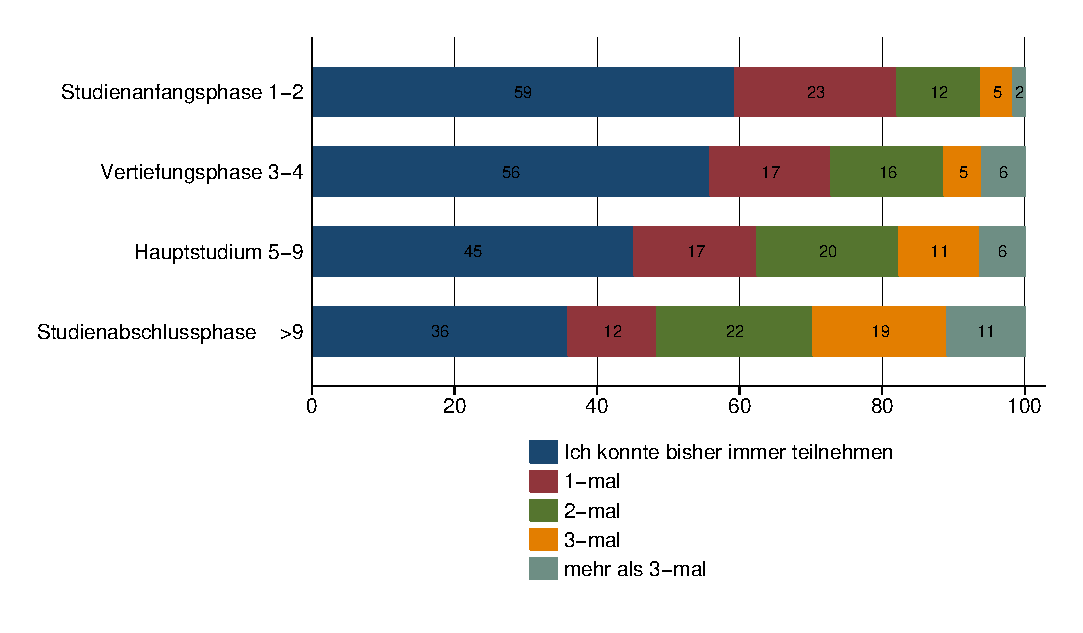
\includegraphics[
%  defaultresolution=72 !,
%  bmpsizefast=false
%]{image}
%\end{verbatim}
% \end{quote}
%
% \subsubsection{Hints}
%
% \begin{itemize}
% \item My version of \xfile{dvips.def} 1999/02/16 v3.0i defines
%       rules for the supported bitmap extensions, but does not
%       include them in the list of extensions that are tried
%       if the file name is not given with an extension.
%       In such a case, the list of extensions can be set
%       by \cs{DeclareGraphicsExtensions}, see \xpackage{grfguide}.
%       The following code just extends the list:
%       \begin{quote}
%\begin{verbatim}
%\makeatletter
%\g@addto@macro\Gin@extensions{,.bmp,.pcx,.msp}
%\makeatother
%\end{verbatim}
%       \end{quote}
% \item My version of \xfile{dvipdfm.def} 1998/11/24 vx.x misses
%       the graphics rule for PNG files. It can be added by:
%       \begin{quote}
%\begin{verbatim}
%\DeclareGraphicsRule{.png}{bmp}{.bb}{#1}
%\end{verbatim}
%       \end{quote}
%       See the previous issue to add the extension \xfile{.png} to the list
%       of extensions for package \xpackage{graphics}.
% \end{itemize}
%
% \subsubsection{Test program}
%
% There is a test program \xfile{bmpsize-test.tex}. Run it through
% \verb|latex|, \verb|pdflatex|, or \verb|pdftex|. Then given
% image files are inspected and the result is printed.
%
% \subsubsection{Interface for programmers}
%
% The macro names of the parsers are \verb|\bmpsize@read@|\meta{type}.
% Example: \cs{bmpsize@read@jpg} in case of JPEG.
%
% A parser sets the switch \cs{ifbmpsize@ok} to true, if it
% could successfully parse the image file.
% The width and height are returnd in \cs{bmpsize@width} and
% \cs{bmpsize@height}. If information about density is available,
% it is used to calculate width and height of the image, otherwise
% the values given by option \xoption{defaultresolution} is used.
% \xoption{resolution} overwrites the values in the image file.
%
% \subsection{Improved bitmap inclusion}
%
% Some drivers for package \xpackage{graphics} define the graphics
% type \xoption{bmp} for bitmap images. The code in the standard
% drivers for \xoption{dvips}, \xoption{dvipdfm}, and \xoption{dvipdfmx}
% is very basic and misses essential features of the
% package \xpackage{graphicx}. Therefore the code for bitmap
% inclusion is automatically rewritten by this package to add
% the following features:
% \begin{itemize}
% \item Support for \xoption{viewport} and \xoption{trim}.
% \item Support for \xoption{clip}.
% \item In case of \xoption{dvipdfm} and \xoption{dvipdfmx} the
%       bitmap images are reused and not included again if they
%       are used more than once.
% \end{itemize}
% However, there is a difference between \xoption{dvipdfm} and
% \xoption{dvipdfmx}, especially if images are reused. In the
% former case the reused box has width and height of 1bp, in the
% latter case its natural width. Thus the correct driver option must be given.
% \xoption{dvipdfm} and \xoption{dvipdfmx} are not equivalent.
%
% Older versions of \xoption{dvipdfmx} uses a size of 1in. However I do
% want to distinguish between versions of the same program. Therefore the
% support of these older versions has stopped with version 1.6 of this package.
% Use version dvipdfmx-20090708 or newer (some few versions before will
% probably also work, but I don't want to investigate this further).
%
% \StopEventually{
% }
%
% \section{Implementation}
%
% \subsection{Basic package \xpackage{bmpsize-base}}
%
%    Identification.
%    \begin{macrocode}
%<*base>
\ProvidesPackage{bmpsize-base}%
  [2009/09/04 v1.6 Basic part of bmpsize (HO)]%
%    \end{macrocode}
%    Modules of package \xpackage{fp} are used for calculations.
%    \begin{macrocode}
\RequirePackage{fp-basic}
\RequirePackage{fp-snap}
%    \end{macrocode}
%    Package \xpackage{fp} uses nested \cs{loop} structures.
%    That breaks with the plain-\TeX\ version of \cs{loop}.
%    Therefore we use the \LaTeX\ variant.
%    \begin{macro}{\@bmpsize@plain@loop}
%    \begin{macrocode}
\long\def\@bmpsize@plain@loop#1\repeat{%
  \def\iterate{%
    #1\relax
    \expandafter\iterate\fi
  }%
  \iterate
  \let\iterate\relax
}
%    \end{macrocode}
%    \end{macro}
%    \begin{macrocode}
\RequirePackage{pdftexcmds}[2007/11/11]
%    \end{macrocode}
%    \begin{macrocode}
\newif\ifbmpsize@ok
\let\@bmpsize@ok\bmpsize@oktrue

\newif\if@bmpsize@bigendian
\newif\if@bmpsize@absnum
\newif\if@bmpsize@user@resolution
\newif\if@bmpsize@fast
\@bmpsize@fasttrue

\def\@bmpsize@init{%
  \let\@bmpsize@org@plain@loop\loop
  \let\loop\@bmpsize@plain@loop
  \bmpsize@okfalse
  \@bmpsize@bigendiantrue
  \@bmpsize@absnumfalse
  \let\bmpsize@pixelwidth\relax
  \let\bmpsize@pixelheight\relax
  \let\bmpsize@pixelx\relax
  \let\bmpsize@pixely\relax
  \let\bmpsize@unit\relax
  \let\bmpsize@pixelxdenom\relax
  \let\bmpsize@pixelydenom\relax
  \let\bmpsize@orientation\relax
}

\def\@bmpsize@stop#1\@nil{}

\def\@bmpsize@loop#1{%
  #1%
  \@bmpsize@loop{#1}%
}
\def\@bmpsize@break#1\@bmpsize@loop#2{}

\def\@bmpsize@size#1#2#3{%
  \edef#3{\pdf@filesize{#1}}%
  \ifx#3\@empty
    \expandafter\@bmpsize@stop
  \fi
  \ifnum#3<#2\relax
    \expandafter\@bmpsize@stop
  \fi
}

\def\@bmpsize@read#1#2#3{%
  \edef\@bmpsize@buf{\pdf@filedump{#3}{#2}{#1}}%
  \edef\@bmpsize@temp{%
    \noexpand\@bmpsize@check@byte{#2}\@bmpsize@buf{}{}\noexpand\\%
  }%
  \@bmpsize@temp
}
\def\@bmpsize@fillbuf#1{%
  \ifx\@bmpsize@buf\@empty
    \expandafter\@firstofone
  \else
    \expandafter\@gobble
  \fi
  {%
    \edef\@bmpsize@buf{%
      \pdf@filedump{\bmpsize@offset}{\bmpsize@fillbuflength}{#1}%
    }%
    \ifx\@bmpsize@buf\@empty
      \expandafter\@bmpsize@stop
    \fi
    \edef\bmpsize@offset{\the\numexpr\bmpsize@offset+\bmpsize@fillbuflength}%
  }%
}
\def\bmpsize@fillbuflength{10}

\def\@bmpsize@append#1#2#3{%
  \edef#1{#2#3}%
}
\def\@bmpsize@pushback#1{%
  \edef\@bmpsize@buf{#1\@bmpsize@buf}%
}

\def\@bmpsize@iswhite#1{%
  \ifnum\pdf@strcmp{#1}{09}=\z@
  \else
    \ifnum\pdf@strcmp{#1}{0A}=\z@
    \else
      \ifnum\pdf@strcmp{#1}{0D}=\z@
      \else
        \ifnum\pdf@strcmp{#1}{20}=\z@
        \else
          1%
        \fi
      \fi
    \fi
  \fi
  \space
}
\def\@bmpsize@isdigit#1{%
  \ifnum\pdf@strcmp{#1}{30}<\z@
    1%
  \else
    \ifnum\pdf@strcmp{#1}{39}>\z@
      1%
    \fi
  \fi
  \space
}

\def\@bmpsize@check@byte#1#2#3{%
  \ifnum#1<\@ne
    \csname fi\endcsname
    \@bmpsize@cleanup@end
  \else
    \csname fi\endcsname
  \ifx!#2#3!%
    \csname fi\endcsname
    \@bmpsize@stop
  \else
    \csname fi\endcsname
    \expandafter\@bmpsize@check@byte\expandafter{\the\numexpr#1-1}%
}
\def\@bmpsize@cleanup@end#1\\{}

\def\@bmpsize@swap@maybe#1{%
  \if@bmpsize@bigendian
  \else
    \edef#1{\expandafter\@bmpsize@@swap#1\@empty\@empty\@empty\@empty}%
  \fi
}
\def\@bmpsize@@swap#1#2#3#4#5#6#7#8{%
  #7#8#5#6#3#4#1#2%
}

\def\@bmpsize@skip@one{%
  \edef\@bmpsize@buf{\expandafter\@gobbletwo\@bmpsize@buf}%
}
\def\@bmpsize@skip@two{%
  \edef\@bmpsize@buf{\expandafter\@gobblefour\@bmpsize@buf}%
}
\def\@bmpsize@skip@four{%
  \edef\@bmpsize@buf{%
    \expandafter\expandafter\expandafter\@gobblefour\expandafter
    \@gobblefour\@bmpsize@buf
  }%
}

\def\@bmpsize@grab#1#2{%
  \edef#1{\noexpand\@bmpsize@grab@byte#2=\@bmpsize@buf\noexpand\\}%
  \edef#1{#1}%
}
\def\@bmpsize@grab@byte#1=#2#3{%
  #2#3%
  \ifnum#1>\@ne
    \expandafter\@bmpsize@grab@byte\the\numexpr#1-1\expandafter=%
  \else
    \expandafter\@bmpsize@cleanup@end
  \fi
}

\def\@bmpsize@abs@maybe#1{%
  \let\@bmpsize@temp\relax
  \if@bmpsize@absnum
    \ifnum"\expandafter\@car#1\@nil>7 %
      \edef#1{\expandafter\@bmpsize@abs@byte#1\relax}%
      \ifnum\pdf@strcmp{#1}{7FFFFFFF}=\z@
        \let\@bmpsize@temp\@bmpsize@stop
      \else
        \def\@bmpsize@temp{\edef#1{\the\numexpr#1+1}}%
      \fi
    \fi
  \fi
}
\def\@bmpsize@abs@byte#1{%
  \ifx#1\relax
  \else
    \ifcase"0#1 %
      F\or E\or D\or C\or B\or A\or 9\or 8\or
      7\or 6\or 5\or 4\or 3\or 2\or 1\or 0%
    \fi
    \expandafter\@bmpsize@abs@byte
  \fi
}

\def\@bmpsize@num@one#1{%
  \@bmpsize@grab#11%
  \@bmpsize@abs@maybe#1%
  \edef#1{\number"#1}%
  \@bmpsize@temp
  \@bmpsize@skip@one
}
\def\@bmpsize@num@two#1{%
  \@bmpsize@grab#12%
  \@bmpsize@swap@maybe#1%
  \@bmpsize@abs@maybe#1%
  \edef#1{\number"#1}%
  \@bmpsize@temp
  \@bmpsize@skip@two
}
\def\@bmpsize@num@four#1{%
  \@bmpsize@grab#14%
  \@bmpsize@swap@maybe#1%
  \@bmpsize@abs@maybe#1%
  \ifnum\pdf@strcmp{#1}{7FFFFFFF}>\z@
    \expandafter\@bmpsize@stop
  \fi
  \edef#1{\number"#1}%
  \@bmpsize@temp
  \@bmpsize@skip@four
}

\def\@bmpsize@div#1#2#3{% #1 := #2/#3
  \FPdiv#1{#2}{#3}%
  \@bmpsize@beautify#1%
}
\def\@bmpsize@beautify#1{%
  \FPifint#1%
    \edef#1{\expandafter\@bmpsize@trunc#1.\@nil}%
  \else
    \edef#1{\expandafter\@bmpsize@cleanup@frac#1.\@nil}%
  \fi
}
\def\@bmpsize@trunc#1.#2\@nil{#1}
% #1 isn't an integer, thus we should have at least one
% necessary digit after the dot
\def\@bmpsize@cleanup@frac#1.#2#3.#4\@nil{%
  #1.#2%
  \ifx\\#3\\%
  \else
    \@bmpsize@cleanup@fracdigits#3000000000\@nil
  \fi
}
\def\@bmpsize@cleanup@fracdigits#1#2#3#4#5#6#7#8#9{%
  \ifcase#9 %
    \ifcase#8 %
      \ifcase#7 %
        \ifcase#6 %
          \ifcase#5 %
            \ifcase #4 %
              \ifcase #3 %
                \ifcase #2 %
                  \ifcase #1 %
                  \else
                    #1%
                  \fi
                \else
                  #1#2%
                \fi
              \else
                #1#2#3%
              \fi
            \else
              #1#2#3#4%
            \fi
          \else
            #1#2#3#4#5%
          \fi
        \else
          #1#2#3#4#5#6%
        \fi
      \else
        #1#2#3#4#5#6#7%
      \fi
    \else
      #1#2#3#4#5#6#7#8%
    \fi
  \else
    #1#2#3#4#5#6#7#8#9%
  \fi
  \@bmpsize@trunc.%
}

\def\@bmpsize@end{%
  \ifbmpsize@ok
    \ifx\bmpsize@pixelwidth\relax
      \bmpsize@okfalse
    \fi
    \ifx\bmpsize@pixelheight\relax
      \bmpsize@okfalse
    \fi
  \fi
  \ifbmpsize@ok
    \ifnum\bmpsize@pixelwidth>\z@
    \else
      \bmpsize@okfalse
    \fi
    \ifnum\bmpsize@pixelheight>\z@
    \else
      \bmpsize@okfalse
    \fi
  \fi
  \ifbmpsize@ok
    \ifcase 0%
      \ifx\bmpsize@pixelx\relax 1 \fi
      \ifx\bmpsize@pixely\relax 1 \fi
      \ifnum\bmpsize@pixelx>\z@\else 1 \fi
      \ifnum\bmpsize@pixely>\z@\else 1 \fi
      \ifx\bmpsize@pixelxdenom\relax
         \ifx\bmpsize@pixelydenom\relax\else 1 \fi
      \else
        \ifnum\bmpsize@pixelxdenom>\z@\else 1 \fi
      \fi
      \ifx\bmpsize@pixelydenom\relax
      \else
        \ifnum\bmpsize@pixelydenom>\z@\else 1 \fi
      \fi
    \else
      \let\bmpsize@pixelx\relax
      \let\bmpsize@pixely\relax
      \let\bmpsize@unit\relax
      \let\bmpsize@pixelxdenom\relax
      \let\bmpsize@pixelydenom\relax
    \fi
    \ifx\bmpsize@pixelxdenom\relax
    \else
      \@bmpsize@div\bmpsize@pixelx\bmpsize@pixelx\bmpsize@pixelxdenom
      \@bmpsize@div\bmpsize@pixely\bmpsize@pixely\bmpsize@pixelydenom
      \let\bmpsize@pixelxdenom\relax
      \let\bmpsize@pixelydenom\relax
    \fi
    \ifcase 0\ifx\bmpsize@unit\relax 1\fi
             \if@bmpsize@user@resolution 1\fi
             \relax
      \let\bmpsize@calc@unit\bmpsize@unit
      \let\bmpsize@calc@pixelx\bmpsize@pixelx
      \let\bmpsize@calc@pixely\bmpsize@pixely
    \else
      \let\bmpsize@calc@unit\bmpsize@unit@default
      \let\bmpsize@calc@pixelx\bmpsize@pixelx@default
      \let\bmpsize@calc@pixely\bmpsize@pixely@default
      \ifx\bmpsize@calc@pixely\Gin@exclamation
        \ifx\bmpsize@pixelx\relax
          \let\bmpsize@calc@pixely\bmpsize@calc@pixelx
        \else
          \FPdiv\bmpsize@calc@pixely\bmpsize@calc@pixelx\bmpsize@pixelx
          \FPmul\bmpsize@calc@pixely\bmpsize@calc@pixely\bmpsize@pixely
        \fi
      \else
        \ifx\bmpsize@calc@pixelx\Gin@exclamation
          \ifx\bmpsize@pixelx\relax
            \let\bmpsize@calc@pixelx\bmpsize@calc@pixely
          \else
            \FPdiv\bmpsize@calc@pixelx\bmpsize@calc@pixely\bmpsize@pixely
            \FPmul\bmpsize@calc@pixelx\bmpsize@calc@pixelx\bmpsize@pixelx
          \fi
        \fi
      \fi
    \fi
    \FPdiv\bmpsize@width\bmpsize@pixelwidth\bmpsize@calc@pixelx
    \FPdiv\bmpsize@height\bmpsize@pixelheight\bmpsize@calc@pixely
    % calculation of width and height in bp for package graphics
    % 1in = 72bp = 72.27pt, 72/72.27 = 8/8.03, 1pt = 65536sp
    \if@bmpsize@fast
      \edef\bmpsize@width{%
        \strip@pt\dimexpr.99626\dimexpr
        \bmpsize@width\dimexpr\bmpsize@calc@unit
      }%
      \edef\bmpsize@height{%
        \strip@pt\dimexpr.99626\dimexpr
        \bmpsize@height\dimexpr\bmpsize@calc@unit
      }%
    \else
      \edef\@bmpsize@temp{\number\dimexpr\bmpsize@calc@unit}%
      \ifnum\@bmpsize@temp>100000 %
        \FPmul\@bmpsize@temp\@bmpsize@temp{0.00001}%
        \def\@bmpsize@corr{100000}%
      \else
        \let\@bmpsize@corr\relax
      \fi
      \FPmul\bmpsize@width\bmpsize@width\@bmpsize@temp
      \FPmul\bmpsize@height\bmpsize@height\@bmpsize@temp
      \FPmul\bmpsize@width\bmpsize@width{8}%
      \FPmul\bmpsize@height\bmpsize@height{8}%
      \FPdiv\bmpsize@width\bmpsize@width{8.03}%
      \FPdiv\bmpsize@height\bmpsize@height{8.03}%
      \FPdiv\bmpsize@width\bmpsize@width{65536}%
      \FPdiv\bmpsize@height\bmpsize@height{65536}%
      \ifx\@bmpsize@corr\relax
      \else
        \FPmul\bmpsize@width\bmpsize@width\@bmpsize@corr
        \FPmul\bmpsize@height\bmpsize@height\@bmpsize@corr
      \fi
      \FPround\bmpsize@width\bmpsize@width{5}%
      \FPround\bmpsize@height\bmpsize@height{5}%
      \@bmpsize@beautify\bmpsize@width
      \@bmpsize@beautify\bmpsize@height
    \fi
  \fi
  \let\loop\@bmpsize@org@plain@loop
}
\def\bmpsize@unit@default{72.27pt}% more accurate than 1in
\def\bmpsize@pixelx@default{72}
\let\bmpsize@pixely@default\Gin@exclamation

\def\bmpsize@types{png,jpg,bmp,gif,tiff,pnm,pam,xpm,tga,pcx,msp,sgi}
%</base>
%    \end{macrocode}
%
% \subsection{Bitmap formats}
%
% \subsubsection{png}
%
%\iffalse
%<*ignore>
%\fi
%\begin{verbatim}
%begin png
%big-endian
%
%read 24 0
%grab 8        -> $temp
%check streq $temp [0x89 "PNG" 0x0D 0x0A 0x1A 0x0A]
%num 4         -> $length
%grab 4        -> $temp
%check streq $temp ["IHDR"]
%num 4         -> $pixelwidth
%num 4         -> $pixelheight
%ok
%assign numexpr(20 + $length) -> $offset
%loop
%  read 8 $offset
%  num 4       -> $length
%  grab 4      -> $temp
%  if streq $temp ["IDAT"]
%    stop
%  fi
%  if streq $temp ["pHYs"]
%    read 9 numexpr($offset + 8)
%    num 4     -> $pixelx
%    num 4     -> $pixely
%    grab 1     -> $temp
%    if numeq $temp 1
%      assign {100cm} -> $unit
%    fi
%    stop
%  fi
%  assign numexpr($offset + 12 + $length) -> $offset
%repeat
%end
%\end{verbatim}
%\iffalse
%</ignore>
%\fi
%    \begin{macro}{\bmpsize@read@png}
%    \begin{macrocode}
%<*base>
\def\bmpsize@read@png#1{%
  \@bmpsize@init
  \@bmpsize@bigendiantrue
  \@bmpsize@read{#1}{24}{0}%
  \@bmpsize@grab\bmpsize@temp{8}%
  \@bmpsize@skip@four
  \@bmpsize@skip@four
  \ifnum\pdf@strcmp{\bmpsize@temp}{89504E470D0A1A0A}=\z@
  \else
    \expandafter\@bmpsize@stop
  \fi
  \@bmpsize@num@four\bmpsize@length
  \@bmpsize@grab\bmpsize@temp{4}%
  \@bmpsize@skip@four
  \ifnum\pdf@strcmp{\bmpsize@temp}{49484452}=\z@
  \else
    \expandafter\@bmpsize@stop
  \fi
  \@bmpsize@num@four\bmpsize@pixelwidth
  \@bmpsize@num@four\bmpsize@pixelheight
  \@bmpsize@ok
  \edef\bmpsize@offset{\the\numexpr20+\bmpsize@length}%
  \@bmpsize@loop{%
    \@bmpsize@read{#1}{8}{\bmpsize@offset}%
    \@bmpsize@num@four\bmpsize@length
    \@bmpsize@grab\bmpsize@temp{4}%
    \@bmpsize@skip@four
    \ifnum\pdf@strcmp{\bmpsize@temp}{49444154}=\z@
      \expandafter\@firstofone
    \else
      \expandafter\@gobble
    \fi
    {%
      \@bmpsize@stop
    }%
    \ifnum\pdf@strcmp{\bmpsize@temp}{70485973}=\z@
      \expandafter\@firstofone
    \else
      \expandafter\@gobble
    \fi
    {%
      \@bmpsize@read{#1}{9}{\numexpr\bmpsize@offset+8\relax}%
      \@bmpsize@num@four\bmpsize@pixelx
      \@bmpsize@num@four\bmpsize@pixely
      \@bmpsize@grab\bmpsize@temp{1}%
      \@bmpsize@skip@one
      \ifnum\bmpsize@temp=1\relax
        \expandafter\@firstofone
      \else
        \expandafter\@gobble
      \fi
      {%
        \def\bmpsize@unit{100cm}%
      }%
      \@bmpsize@stop
    }%
    \edef\bmpsize@offset{\the\numexpr\bmpsize@offset+12+\bmpsize@length}%
  }%
  \@bmpsize@stop
  \@nil
  \@bmpsize@end
}%
%</base>
%    \end{macrocode}
%    \end{macro}
%
% \subsubsection{jpg}
%
%\iffalse
%<*ignore>
%\fi
%\begin{verbatim}
%begin jpg
%
%read 3 0
%grab 3      -> $temp % SOI and 0xFF
%check streq $temp [0xFF 0xD8 0xFF]
%assign {2} -> $offset
%assign {0} -> $exifdensity
%loop
%  read 4 $offset
%  grab 1    -> $temp
%  check streq $temp [0xFF]
%  num 1    -> $temp
%  if numeq $temp 0xDA % SOS
%    stop
%  fi
%  % look for JFIF APP0 segment
%  if numeq $temp 0xE0 % APP0
%    num 2       -> $length
%    if numeq $exifdensity 0
%      if numge $length 16 % a JFIF segment has 16 bytes at least
%        read 12 numexpr($offset + 4)
%        grab 5      -> $temp % identifier
%        if streq $temp ["JFIF" 0x0]
%          check numge $length 16
%          skip 2 % version
%          num 1       -> $temp % units
%          if numeq $temp 1
%            assign {72.27pt} -> $unit
%          else
%            if numeq $temp 2
%              assign {1cm} -> $unit
%            fi
%          fi
%          num 2    -> $pixelx
%          num 2    -> $pixely
%        fi
%      fi
%    fi
%  else
%    if numeq $temp 0xE1 % APP1
%      % look for Exif APP1 segment
%      num 2 -> $length
%      if numge $length 20 % identifier (6) + Tiff header (8) + first IFD (>=6)
%        read 20 numexpr($offset + 4)
%        grab 6 -> $temp
%        if streq $temp ["Exif" 0x0 0x0]
%          assign numexpr($offset + 10) -> $exifoffset
%          % read TIFF header
%          grab 2 -> $temp
%          if streq $temp ["II"]
%            little-endian
%          else
%            check streq $temp ["MM"]
%            % big-endian
%          fi
%          num 2 -> $temp
%          check numeq $temp 42
%          num 4 -> $temp % offset of first IFD
%          check numgt $temp 0
%          % read first IFD
%          assign numexpr($temp + $exifoffset) -> $off
%          read 2 $off
%          num 2 -> $entries
%          assign numexpr($off + 2) -> $off
%          loop
%            if numeq $entries 0
%              break
%            fi
%            assign numexpr($entries - 1) -> $entries
%            % entry format:
%            % 2 tag
%            % 2 field type
%            % 4 count
%            % 4 value/offset
%            read 12 $off
%            assign numexpr($off + 12) -> $off
%            num 2 -> $tag
%            if numeq $tag 296 % ResolutionUnit
%              skip 6 % type: 3 (short), count: 1
%              num 2 -> $temp
%              ifcase $temp
%              or % 1
%                clear $unit
%              or % 2
%                assign {72.27pt} -> $unit
%              or % 3
%                assign {1cm} -> $unit
%              else
%                clear $unit % unknown
%              fi
%              ifcase $temp
%              or % 1
%              or % 2
%                assign {1} -> $exifdensity
%              or % 3
%                assign {1} -> $exifdensity
%              else
%                assign $exifdensity -> $exifdensity
%              fi
%            fi
%            % 256 ImageWidth (use width of JPG part)
%            % 257 ImageHeight (use height of JPG part)
%            if numeq $tag 274 % Orientation
%              skip 6 % type: 3 (short), count: 1
%              num 2 -> $temp
%              if numge $temp 0 
%                if numle $temp 8
%                  assign $temp -> $orientation
%                fi
%              fi
%            fi
%            if numeq $tag 282 % XResolution
%              skip 6
%              num 4 -> $temp
%              read 8 numexpr($temp + $exifoffset)
%              num 4 -> $pixelx
%              num 4 -> $temp
%              if numeq $temp 1
%              else
%                assign numexpr($temp) -> $pixelxdenom
%                % div $pixelx $temp -> $pixelx
%              fi
%            fi
%            if numeq $tag 283 % YResolution
%              skip 6
%              num 4 -> $temp
%              read 8 numexpr($temp + $exifoffset)
%              num 4 -> $pixely
%              num 4 -> $temp
%              if numeq $temp 1
%              else
%                assign numexpr($temp) -> $pixelydenom
%                % div $pixely $temp -> $pixely
%              fi
%            fi
%          repeat
%          big-endian
%        fi
%      fi
%    else
%      assign numexpr($temp - 0xC0) -> $temp
%      ifcase $temp % SOF_0
%      or % SOF_1
%      or % SOF_2
%      or % SOF_3
%      or % DHT
%        assign {-1} -> $temp
%      or % SOF_5
%      or % SOF_6
%      or % SOF_7
%      or % JPG
%        assign {-1} -> $temp
%      or % SOF_9
%      or % SOF_10
%      or % SOF_11
%      or % DAC
%        assign {-1} -> $temp
%      or % SOF_13
%      or % SOF_14
%      or % SOF_15
%      else
%        assign {-1} -> $temp
%      fi
%      if numeq $temp -1
%      else
%        read 4 numexpr($offset + 5)
%        num 2  -> $pixelheight
%        num 2  -> $pixelwidth
%        if numeq $pixelheight 0
%          clear $pixelheight
%          stop
%        fi
%        ok
%        stop
%      fi
%      num 2 -> $length
%    fi
%  fi
%  assign numexpr($offset + $length + 2) -> $offset
%repeat
%end
%\end{verbatim}
%\iffalse
%</ignore>
%\fi
%    \begin{macro}{\bmpsize@read@jpg}
%    \begin{macrocode}
%<*base>
\def\bmpsize@read@jpg#1{%
  \@bmpsize@init
  \@bmpsize@read{#1}{3}{0}%
  \@bmpsize@grab\bmpsize@temp{3}%
  \@bmpsize@skip@two
  \@bmpsize@skip@one
  \ifnum\pdf@strcmp{\bmpsize@temp}{FFD8FF}=\z@
  \else
    \expandafter\@bmpsize@stop
  \fi
  \def\bmpsize@offset{2}%
  \def\bmpsize@exifdensity{0}%
  \@bmpsize@loop{%
    \@bmpsize@read{#1}{4}{\bmpsize@offset}%
    \@bmpsize@grab\bmpsize@temp{1}%
    \@bmpsize@skip@one
    \ifnum\pdf@strcmp{\bmpsize@temp}{FF}=\z@
    \else
      \expandafter\@bmpsize@stop
    \fi
    \@bmpsize@num@one\bmpsize@temp
    \ifnum\bmpsize@temp=218\relax
      \expandafter\@firstofone
    \else
      \expandafter\@gobble
    \fi
    {%
      \@bmpsize@stop
    }%
    \ifnum\bmpsize@temp=224\relax
      \expandafter\@firstoftwo
    \else
      \expandafter\@secondoftwo
    \fi
    {%
      \@bmpsize@num@two\bmpsize@length
      \ifnum\bmpsize@exifdensity=0\relax
        \expandafter\@firstofone
      \else
        \expandafter\@gobble
      \fi
      {%
        \unless\ifnum\bmpsize@length<16\relax
          \expandafter\@firstofone
        \else
          \expandafter\@gobble
        \fi
        {%
          \@bmpsize@read{#1}{12}{\numexpr\bmpsize@offset+4\relax}%
          \@bmpsize@grab\bmpsize@temp{5}%
          \@bmpsize@skip@four
          \@bmpsize@skip@one
          \ifnum\pdf@strcmp{\bmpsize@temp}{4A46494600}=\z@
            \expandafter\@firstofone
          \else
            \expandafter\@gobble
          \fi
          {%
            \ifnum\bmpsize@length<16\relax
              \expandafter\@bmpsize@stop
            \fi
            \@bmpsize@skip@two
            \@bmpsize@num@one\bmpsize@temp
            \ifnum\bmpsize@temp=1\relax
              \expandafter\@firstoftwo
            \else
              \expandafter\@secondoftwo
            \fi
            {%
              \def\bmpsize@unit{72.27pt}%
            }{%
              \ifnum\bmpsize@temp=2\relax
                \expandafter\@firstofone
              \else
                \expandafter\@gobble
              \fi
              {%
                \def\bmpsize@unit{1cm}%
              }%
            }%
            \@bmpsize@num@two\bmpsize@pixelx
            \@bmpsize@num@two\bmpsize@pixely
          }%
        }%
      }%
    }{%
      \ifnum\bmpsize@temp=225\relax
        \expandafter\@firstoftwo
      \else
        \expandafter\@secondoftwo
      \fi
      {%
        \@bmpsize@num@two\bmpsize@length
        \unless\ifnum\bmpsize@length<20\relax
          \expandafter\@firstofone
        \else
          \expandafter\@gobble
        \fi
        {%
          \@bmpsize@read{#1}{20}{\numexpr\bmpsize@offset+4\relax}%
          \@bmpsize@grab\bmpsize@temp{6}%
          \@bmpsize@skip@four
          \@bmpsize@skip@two
          \ifnum\pdf@strcmp{\bmpsize@temp}{457869660000}=\z@
            \expandafter\@firstofone
          \else
            \expandafter\@gobble
          \fi
          {%
            \edef\bmpsize@exifoffset{\the\numexpr\bmpsize@offset+10}%
            \@bmpsize@grab\bmpsize@temp{2}%
            \@bmpsize@skip@two
            \ifnum\pdf@strcmp{\bmpsize@temp}{4949}=\z@
              \expandafter\@firstoftwo
            \else
              \expandafter\@secondoftwo
            \fi
            {%
              \@bmpsize@bigendianfalse
            }{%
              \ifnum\pdf@strcmp{\bmpsize@temp}{4D4D}=\z@
              \else
                \expandafter\@bmpsize@stop
              \fi
            }%
            \@bmpsize@num@two\bmpsize@temp
            \ifnum\bmpsize@temp=42\relax
            \else
              \expandafter\@bmpsize@stop
            \fi
            \@bmpsize@num@four\bmpsize@temp
            \ifnum\bmpsize@temp>0\relax
            \else
              \expandafter\@bmpsize@stop
            \fi
            \edef\bmpsize@off{\the\numexpr\bmpsize@temp+\bmpsize@exifoffset}%
            \@bmpsize@read{#1}{2}{\bmpsize@off}%
            \@bmpsize@num@two\bmpsize@entries
            \edef\bmpsize@off{\the\numexpr\bmpsize@off+2}%
            \@bmpsize@loop{%
              \ifnum\bmpsize@entries=0\relax
                \expandafter\@firstofone
              \else
                \expandafter\@gobble
              \fi
              {%
                \@bmpsize@break
              }%
              \edef\bmpsize@entries{\the\numexpr\bmpsize@entries-1}%
              \@bmpsize@read{#1}{12}{\bmpsize@off}%
              \edef\bmpsize@off{\the\numexpr\bmpsize@off+12}%
              \@bmpsize@num@two\bmpsize@tag
              \ifnum\bmpsize@tag=296\relax
                \expandafter\@firstofone
              \else
                \expandafter\@gobble
              \fi
              {%
                \@bmpsize@skip@four
                \@bmpsize@skip@two
                \@bmpsize@num@two\bmpsize@temp
                \ifcase\bmpsize@temp\relax
                \or
                  \let\bmpsize@unit\relax
                \or
                  \def\bmpsize@unit{72.27pt}%
                \or
                  \def\bmpsize@unit{1cm}%
                \else
                  \let\bmpsize@unit\relax
                \fi
                \ifcase\bmpsize@temp\relax
                \or
                \or
                  \def\bmpsize@exifdensity{1}%
                \or
                  \def\bmpsize@exifdensity{1}%
                \else
                  \let\bmpsize@exifdensity\bmpsize@exifdensity
                \fi
              }%
              \ifnum\bmpsize@tag=274\relax
                \expandafter\@firstofone
              \else
                \expandafter\@gobble
              \fi
              {%
                \@bmpsize@skip@four
                \@bmpsize@skip@two
                \@bmpsize@num@two\bmpsize@temp
                \unless\ifnum\bmpsize@temp<0\relax
                  \expandafter\@firstofone
                \else
                  \expandafter\@gobble
                \fi
                {%
                  \unless\ifnum\bmpsize@temp>8\relax
                    \expandafter\@firstofone
                  \else
                    \expandafter\@gobble
                  \fi
                  {%
                    \let\bmpsize@orientation\bmpsize@temp
                  }%
                }%
              }%
              \ifnum\bmpsize@tag=282\relax
                \expandafter\@firstofone
              \else
                \expandafter\@gobble
              \fi
              {%
                \@bmpsize@skip@four
                \@bmpsize@skip@two
                \@bmpsize@num@four\bmpsize@temp
                \@bmpsize@read{#1}{8}{\numexpr\bmpsize@temp+\bmpsize@exifoffset\relax}%
                \@bmpsize@num@four\bmpsize@pixelx
                \@bmpsize@num@four\bmpsize@temp
                \ifnum\bmpsize@temp=1\relax
                  \expandafter\@gobble
                \else
                  \expandafter\@firstofone
                \fi
                {%
                  \edef\bmpsize@pixelxdenom{\the\numexpr\bmpsize@temp}%
                }%
              }%
              \ifnum\bmpsize@tag=283\relax
                \expandafter\@firstofone
              \else
                \expandafter\@gobble
              \fi
              {%
                \@bmpsize@skip@four
                \@bmpsize@skip@two
                \@bmpsize@num@four\bmpsize@temp
                \@bmpsize@read{#1}{8}{\numexpr\bmpsize@temp+\bmpsize@exifoffset\relax}%
                \@bmpsize@num@four\bmpsize@pixely
                \@bmpsize@num@four\bmpsize@temp
                \ifnum\bmpsize@temp=1\relax
                  \expandafter\@gobble
                \else
                  \expandafter\@firstofone
                \fi
                {%
                  \edef\bmpsize@pixelydenom{\the\numexpr\bmpsize@temp}%
                }%
              }%
            }%
            \@bmpsize@bigendiantrue
          }%
        }%
      }{%
        \edef\bmpsize@temp{\the\numexpr\bmpsize@temp-192}%
        \ifcase\bmpsize@temp\relax
        \or
        \or
        \or
        \or
          \def\bmpsize@temp{-1}%
        \or
        \or
        \or
        \or
          \def\bmpsize@temp{-1}%
        \or
        \or
        \or
        \or
          \def\bmpsize@temp{-1}%
        \or
        \or
        \or
        \else
          \def\bmpsize@temp{-1}%
        \fi
        \ifnum\bmpsize@temp=-1\relax
          \expandafter\@gobble
        \else
          \expandafter\@firstofone
        \fi
        {%
          \@bmpsize@read{#1}{4}{\numexpr\bmpsize@offset+5\relax}%
          \@bmpsize@num@two\bmpsize@pixelheight
          \@bmpsize@num@two\bmpsize@pixelwidth
          \ifnum\bmpsize@pixelheight=0\relax
            \expandafter\@firstofone
          \else
            \expandafter\@gobble
          \fi
          {%
            \let\bmpsize@pixelheight\relax
            \@bmpsize@stop
          }%
          \@bmpsize@ok
          \@bmpsize@stop
        }%
        \@bmpsize@num@two\bmpsize@length
      }%
    }%
    \edef\bmpsize@offset{\the\numexpr\bmpsize@offset+\bmpsize@length+2}%
  }%
  \@bmpsize@stop
  \@nil
  \@bmpsize@end
}%
%</base>
%    \end{macrocode}
%    \end{macro}
%
% \subsubsection{bmp}
%
%\iffalse
%<*ignore>
%\fi
%\begin{verbatim}
%begin bmp
%little-endian
%
%read 26 0
%grab 2 -> $temp
%check streq $temp ["BM"]
%skip 12
%% header size is 4 bytes in V3+, unknown for V1, V2,
%% known header sizes fit in 2 bytes
%num 2   -> $temp
%if numeq $temp 12 % V1
%  skip 2
%  num 2 -> $pixelwidth
%  num 2 -> $pixelheight
%  % no resolution entries
%  ok
%  stop
%fi
%if numeq $temp 64 % V2
%  skip 2
%  num 2 -> $pixelwidth
%  num 2 -> $pixelheight
%  % missing specification for resolution
%  ok
%  stop
%fi
%% V3, V4, V5
%skip 2
%num 4 -> $pixelwidth
%absnum 4 -> $pixelheight
%ok
%read 8 38
%num 4 -> $pixelx
%num 4 -> $pixely
%assign {100cm} -> $unit
%end
%\end{verbatim}
%\iffalse
%</ignore>
%\fi
%    \begin{macro}{\bmpsize@read@bmp}
%    \begin{macrocode}
%<*base>
\def\bmpsize@read@bmp#1{%
  \@bmpsize@init
  \@bmpsize@bigendianfalse
  \@bmpsize@read{#1}{26}{0}%
  \@bmpsize@grab\bmpsize@temp{2}%
  \@bmpsize@skip@two
  \ifnum\pdf@strcmp{\bmpsize@temp}{424D}=\z@
  \else
    \expandafter\@bmpsize@stop
  \fi
  \@bmpsize@skip@four
  \@bmpsize@skip@four
  \@bmpsize@skip@four
  \@bmpsize@num@two\bmpsize@temp
  \ifnum\bmpsize@temp=12\relax
    \expandafter\@firstofone
  \else
    \expandafter\@gobble
  \fi
  {%
    \@bmpsize@skip@two
    \@bmpsize@num@two\bmpsize@pixelwidth
    \@bmpsize@num@two\bmpsize@pixelheight
    \@bmpsize@ok
    \@bmpsize@stop
  }%
  \ifnum\bmpsize@temp=64\relax
    \expandafter\@firstofone
  \else
    \expandafter\@gobble
  \fi
  {%
    \@bmpsize@skip@two
    \@bmpsize@num@two\bmpsize@pixelwidth
    \@bmpsize@num@two\bmpsize@pixelheight
    \@bmpsize@ok
    \@bmpsize@stop
  }%
  \@bmpsize@skip@two
  \@bmpsize@num@four\bmpsize@pixelwidth
  \@bmpsize@absnumtrue
  \@bmpsize@num@four\bmpsize@pixelheight
  \@bmpsize@absnumfalse
  \@bmpsize@ok
  \@bmpsize@read{#1}{8}{38}%
  \@bmpsize@num@four\bmpsize@pixelx
  \@bmpsize@num@four\bmpsize@pixely
  \def\bmpsize@unit{100cm}%
  \@bmpsize@stop
  \@nil
  \@bmpsize@end
}%
%</base>
%    \end{macrocode}
%    \end{macro}
%
% \subsubsection{gif}
%
%\iffalse
%<*ignore>
%\fi
%\begin{verbatim}
%begin gif
%little-endian
%
%% Header
%read 13 0
%grab 3      -> $temp
%check streq $temp ["GIF"]
%skip 3      % version
%
%% Logical Screen Descriptor
%num 2       -> $pixelwidth
%num 2       -> $pixelheight
%skip 2
%num 1       -> $temp % Pixel Aspect Ratio
%if numeq $temp 0
%else
%  assign numexpr($temp + 15) -> $pixelx
%  assign {64}     -> $pixely
%fi
%ok
%end
%\end{verbatim}
%\iffalse
%</ignore>
%\fi
%    \begin{macro}{\bmpsize@read@gif}
%    \begin{macrocode}
%<*base>
\def\bmpsize@read@gif#1{%
  \@bmpsize@init
  \@bmpsize@bigendianfalse
  \@bmpsize@read{#1}{13}{0}%
  \@bmpsize@grab\bmpsize@temp{3}%
  \@bmpsize@skip@two
  \@bmpsize@skip@one
  \ifnum\pdf@strcmp{\bmpsize@temp}{474946}=\z@
  \else
    \expandafter\@bmpsize@stop
  \fi
  \@bmpsize@skip@two
  \@bmpsize@skip@one
  \@bmpsize@num@two\bmpsize@pixelwidth
  \@bmpsize@num@two\bmpsize@pixelheight
  \@bmpsize@skip@two
  \@bmpsize@num@one\bmpsize@temp
  \ifnum\bmpsize@temp=0\relax
    \expandafter\@gobble
  \else
    \expandafter\@firstofone
  \fi
  {%
    \edef\bmpsize@pixelx{\the\numexpr\bmpsize@temp+15}%
    \def\bmpsize@pixely{64}%
  }%
  \@bmpsize@ok
  \@bmpsize@stop
  \@nil
  \@bmpsize@end
}%
%</base>
%    \end{macrocode}
%    \end{macro}
%
% \subsubsection{tiff}
%
%\iffalse
%<*ignore>
%\fi
%\begin{verbatim}
%begin tiff
%% defaults
%assign {72.27pt} -> $unit
%
%% Image File Header
%read 8 0
%grab 2 -> $temp
%if streq $temp ["II"]
%  little-endian
%else
%  check streq $temp ["MM"]
%  big-endian
%fi
%num 2 -> $temp
%check numeq $temp 42
%num 4 -> $offset % first IFD (Image File Directory)
%
%% First IFD
%read 2 $offset
%assign numexpr($offset + 2) -> $offset
%num 2 -> $entries
%ok % must rely on checks at the end
%loop
%  if numeq $entries 0
%    stop
%  fi
%  assign numexpr($entries - 1) -> $entries
%  % entry format:
%  % 2 tag
%  % 2 field type
%  % 4 count
%  % 4 value/offset
%  read 12 $offset
%  assign numexpr($offset + 12) -> $offset
%  num 2 -> $tag % tag
%  if numeq $temp 296 % ResolutionUnit
%    skip 6 % type: 3 (short), count: 1
%    num 2 -> $temp
%    ifcase $temp
%    or % 1
%      clear $unit
%    or % 2
%      assign {72.27pt} -> $unit
%    or % 3
%      assign {1cm} -> $unit
%    else
%      clear $unit
%    fi
%  fi
%  if numeq $tag 256 % ImageWidth
%    skip 6
%    num 4 -> $pixelwidth
%  fi
%  if numeq $tag 257 % ImageLength
%    skip 6
%    num 4 -> $pixelheight
%  fi
%  if numeq $tag 282 % XResolution
%    skip 6
%    num 4 -> $temp
%    read 8 $temp
%    num 4 -> $pixelx
%    num 4 -> $temp
%    if numeq $temp 1
%    else
%      assign numexpr($temp) -> $pixelxdenom
%      % div $pixelx $temp -> $pixelx
%    fi
%  fi
%  if numeq $tag 283 % YResolution
%    skip 6
%    num 4 -> $temp
%    read 8 $temp
%    num 4 -> $pixely
%    num 4 -> $temp
%    if numeq $temp 1
%    else
%      assign numexpr($temp) -> $pixelydenom
%      % div $pixely $temp -> $pixely
%    fi
%  fi
%repeat
%end
%\end{verbatim}
%\iffalse
%</ignore>
%\fi
%    \begin{macro}{\bmpsize@read@tiff}
%    \begin{macrocode}
%<*base>
\def\bmpsize@read@tiff#1{%
  \@bmpsize@init
  \def\bmpsize@unit{72.27pt}%
  \@bmpsize@read{#1}{8}{0}%
  \@bmpsize@grab\bmpsize@temp{2}%
  \@bmpsize@skip@two
  \ifnum\pdf@strcmp{\bmpsize@temp}{4949}=\z@
    \expandafter\@firstoftwo
  \else
    \expandafter\@secondoftwo
  \fi
  {%
    \@bmpsize@bigendianfalse
  }{%
    \ifnum\pdf@strcmp{\bmpsize@temp}{4D4D}=\z@
    \else
      \expandafter\@bmpsize@stop
    \fi
    \@bmpsize@bigendiantrue
  }%
  \@bmpsize@num@two\bmpsize@temp
  \ifnum\bmpsize@temp=42\relax
  \else
    \expandafter\@bmpsize@stop
  \fi
  \@bmpsize@num@four\bmpsize@offset
  \@bmpsize@read{#1}{2}{\bmpsize@offset}%
  \edef\bmpsize@offset{\the\numexpr\bmpsize@offset+2}%
  \@bmpsize@num@two\bmpsize@entries
  \@bmpsize@ok
  \@bmpsize@loop{%
    \ifnum\bmpsize@entries=0\relax
      \expandafter\@firstofone
    \else
      \expandafter\@gobble
    \fi
    {%
      \@bmpsize@stop
    }%
    \edef\bmpsize@entries{\the\numexpr\bmpsize@entries-1}%
    \@bmpsize@read{#1}{12}{\bmpsize@offset}%
    \edef\bmpsize@offset{\the\numexpr\bmpsize@offset+12}%
    \@bmpsize@num@two\bmpsize@tag
    \ifnum\bmpsize@temp=296\relax
      \expandafter\@firstofone
    \else
      \expandafter\@gobble
    \fi
    {%
      \@bmpsize@skip@four
      \@bmpsize@skip@two
      \@bmpsize@num@two\bmpsize@temp
      \ifcase\bmpsize@temp\relax
      \or
        \let\bmpsize@unit\relax
      \or
        \def\bmpsize@unit{72.27pt}%
      \or
        \def\bmpsize@unit{1cm}%
      \else
        \let\bmpsize@unit\relax
      \fi
    }%
    \ifnum\bmpsize@tag=256\relax
      \expandafter\@firstofone
    \else
      \expandafter\@gobble
    \fi
    {%
      \@bmpsize@skip@four
      \@bmpsize@skip@two
      \@bmpsize@num@four\bmpsize@pixelwidth
    }%
    \ifnum\bmpsize@tag=257\relax
      \expandafter\@firstofone
    \else
      \expandafter\@gobble
    \fi
    {%
      \@bmpsize@skip@four
      \@bmpsize@skip@two
      \@bmpsize@num@four\bmpsize@pixelheight
    }%
    \ifnum\bmpsize@tag=282\relax
      \expandafter\@firstofone
    \else
      \expandafter\@gobble
    \fi
    {%
      \@bmpsize@skip@four
      \@bmpsize@skip@two
      \@bmpsize@num@four\bmpsize@temp
      \@bmpsize@read{#1}{8}{\bmpsize@temp}%
      \@bmpsize@num@four\bmpsize@pixelx
      \@bmpsize@num@four\bmpsize@temp
      \ifnum\bmpsize@temp=1\relax
        \expandafter\@gobble
      \else
        \expandafter\@firstofone
      \fi
      {%
        \edef\bmpsize@pixelxdenom{\the\numexpr\bmpsize@temp}%
      }%
    }%
    \ifnum\bmpsize@tag=283\relax
      \expandafter\@firstofone
    \else
      \expandafter\@gobble
    \fi
    {%
      \@bmpsize@skip@four
      \@bmpsize@skip@two
      \@bmpsize@num@four\bmpsize@temp
      \@bmpsize@read{#1}{8}{\bmpsize@temp}%
      \@bmpsize@num@four\bmpsize@pixely
      \@bmpsize@num@four\bmpsize@temp
      \ifnum\bmpsize@temp=1\relax
        \expandafter\@gobble
      \else
        \expandafter\@firstofone
      \fi
      {%
        \edef\bmpsize@pixelydenom{\the\numexpr\bmpsize@temp}%
      }%
    }%
  }%
  \@bmpsize@stop
  \@nil
  \@bmpsize@end
}%
%</base>
%    \end{macrocode}
%    \end{macro}
%
% \subsubsection{pnm}
%
%\iffalse
%<*ignore>
%\fi
%\begin{verbatim}
%begin pnm
%assign {0} -> $offset
%read 3 $offset
%assign {3} -> $offset
%grab 1 -> $temp
%check streq $temp ["P"]
%grab 1 -> $temp
%check strge $temp ["1"]
%check strle $temp ["6"]
%% ensure one white space
%grab 1 -> $temp
%if iswhite $temp
%else
%  stop
%fi
%loop
%  % skip white space
%  fillbuf
%  grab 1 -> $temp
%  if iswhite $temp
%  else
%    if streq $temp ["#"]
%      % ignore comments
%      loop
%        fillbuf
%        grab 1 -> $temp
%        if streq $temp [0x0A]
%          break
%        else
%          if streq $temp [0x0D]
%            break
%          fi
%        fi
%      repeat
%    else
%      pushback $temp
%      break
%    fi
%  fi
%repeat
%assign {} -> $tempnum
%loop
%  fillbuf
%  grab 1 -> $temp
%  if isdigit $temp
%    append $tempnum $temp -> $tempnum
%  else
%    if iswhite $temp
%      break
%    else
%      stop
%    fi
%  fi
%repeat
%assign unescapehex($tempnum) -> $pixelwidth
%loop
%  fillbuf
%  grab 1 -> $temp
%  if iswhite $temp
%  else
%    pushback $temp
%    break
%  fi
%repeat
%assign {} -> $tempnum
%loop
%  fillbuf
%  grab 1 -> $temp
%  if isdigit $temp
%    append $tempnum $temp -> $tempnum
%  else
%    if iswhite $temp
%      break
%    else
%      stop
%    fi
%  fi
%repeat
%assign unescapehex($tempnum) -> $pixelheight
%ok
%end
%\end{verbatim}
%\iffalse
%</ignore>
%\fi
%    \begin{macro}{\bmpsize@read@pnm}
%    \begin{macrocode}
%<*base>
\def\bmpsize@read@pnm#1{%
  \@bmpsize@init
  \def\bmpsize@offset{0}%
  \@bmpsize@read{#1}{3}{\bmpsize@offset}%
  \def\bmpsize@offset{3}%
  \@bmpsize@grab\bmpsize@temp{1}%
  \@bmpsize@skip@one
  \ifnum\pdf@strcmp{\bmpsize@temp}{50}=\z@
  \else
    \expandafter\@bmpsize@stop
  \fi
  \@bmpsize@grab\bmpsize@temp{1}%
  \@bmpsize@skip@one
  \ifnum\pdf@strcmp{\bmpsize@temp}{31}<\z@
    \expandafter\@bmpsize@stop
  \fi
  \ifnum\pdf@strcmp{\bmpsize@temp}{36}>\z@
    \expandafter\@bmpsize@stop
  \fi
  \@bmpsize@grab\bmpsize@temp{1}%
  \@bmpsize@skip@one
  \ifcase 0\@bmpsize@iswhite\bmpsize@temp
    \expandafter\@gobble
  \else
    \expandafter\@firstofone
  \fi
  {%
    \@bmpsize@stop
  }%
  \@bmpsize@loop{%
    \@bmpsize@fillbuf{#1}%
    \@bmpsize@grab\bmpsize@temp{1}%
    \@bmpsize@skip@one
    \ifcase 0\@bmpsize@iswhite\bmpsize@temp
      \expandafter\@gobble
    \else
      \expandafter\@firstofone
    \fi
    {%
      \ifnum\pdf@strcmp{\bmpsize@temp}{23}=\z@
        \expandafter\@firstoftwo
      \else
        \expandafter\@secondoftwo
      \fi
      {%
        \@bmpsize@loop{%
          \@bmpsize@fillbuf{#1}%
          \@bmpsize@grab\bmpsize@temp{1}%
          \@bmpsize@skip@one
          \ifnum\pdf@strcmp{\bmpsize@temp}{0A}=\z@
            \expandafter\@firstoftwo
          \else
            \expandafter\@secondoftwo
          \fi
          {%
            \@bmpsize@break
          }{%
            \ifnum\pdf@strcmp{\bmpsize@temp}{0D}=\z@
              \expandafter\@firstofone
            \else
              \expandafter\@gobble
            \fi
            {%
              \@bmpsize@break
            }%
          }%
        }%
      }{%
        \@bmpsize@pushback\bmpsize@temp
        \@bmpsize@break
      }%
    }%
  }%
  \def\bmpsize@tempnum{}%
  \@bmpsize@loop{%
    \@bmpsize@fillbuf{#1}%
    \@bmpsize@grab\bmpsize@temp{1}%
    \@bmpsize@skip@one
    \ifcase 0\@bmpsize@isdigit\bmpsize@temp
      \expandafter\@firstoftwo
    \else
      \expandafter\@secondoftwo
    \fi
    {%
      \@bmpsize@append\bmpsize@tempnum\bmpsize@tempnum\bmpsize@temp
    }{%
      \ifcase 0\@bmpsize@iswhite\bmpsize@temp
        \expandafter\@firstoftwo
      \else
        \expandafter\@secondoftwo
      \fi
      {%
        \@bmpsize@break
      }{%
        \@bmpsize@stop
      }%
    }%
  }%
  \edef\bmpsize@pixelwidth{\pdf@unescapehex{\bmpsize@tempnum}}%
  \@bmpsize@loop{%
    \@bmpsize@fillbuf{#1}%
    \@bmpsize@grab\bmpsize@temp{1}%
    \@bmpsize@skip@one
    \ifcase 0\@bmpsize@iswhite\bmpsize@temp
      \expandafter\@gobble
    \else
      \expandafter\@firstofone
    \fi
    {%
      \@bmpsize@pushback\bmpsize@temp
      \@bmpsize@break
    }%
  }%
  \def\bmpsize@tempnum{}%
  \@bmpsize@loop{%
    \@bmpsize@fillbuf{#1}%
    \@bmpsize@grab\bmpsize@temp{1}%
    \@bmpsize@skip@one
    \ifcase 0\@bmpsize@isdigit\bmpsize@temp
      \expandafter\@firstoftwo
    \else
      \expandafter\@secondoftwo
    \fi
    {%
      \@bmpsize@append\bmpsize@tempnum\bmpsize@tempnum\bmpsize@temp
    }{%
      \ifcase 0\@bmpsize@iswhite\bmpsize@temp
        \expandafter\@firstoftwo
      \else
        \expandafter\@secondoftwo
      \fi
      {%
        \@bmpsize@break
      }{%
        \@bmpsize@stop
      }%
    }%
  }%
  \edef\bmpsize@pixelheight{\pdf@unescapehex{\bmpsize@tempnum}}%
  \@bmpsize@ok
  \@bmpsize@stop
  \@nil
  \@bmpsize@end
}%
%</base>
%    \end{macrocode}
%    \end{macro}
%
% \subsubsection{pam}
%
%\iffalse
%<*ignore>
%\fi
%\begin{verbatim}
%begin pam
%read 3 0
%assign {3} -> $offset
%assign $offset -> $off
%grab 3 -> $temp
%check streq $temp ["P7" 0x0A]
%loop
%  fillbuf
%  grab 1 -> $temp
%  if iswhite $temp
%    % ignore white space
%    assign numexpr($off + 1) -> $off
%  else
%    if streq $temp ["#"]
%      % ignore comment line
%      assign numexpr($off + 1) -> $off
%      loop
%        fillbuf
%        grab 1 -> $temp
%        assign numexpr($off + 1) -> $off
%        if streq $temp [0x0A]
%          break
%        fi
%      repeat
%    else
%      read 6 $off
%      assign numexpr($off + 6) -> $offset
%      grab 5 -> $head
%      if streq $head ["WIDTH"]
%        assign numexpr($off + 5) -> $off
%        % skip white space
%        loop
%          fillbuf
%          grab 1 -> $temp
%          if iswhite $temp
%            assign numexpr($off + 1) -> $off
%          else
%            if isdigit $temp
%              assign numexpr($off + 1) -> $off
%              break
%            else
%              % error
%              stop
%            fi
%          fi
%        repeat
%        % read number
%        assign $temp -> $tempnum
%        loop
%          fillbuf
%          grab 1 -> $temp
%          if isdigit $temp
%            assign numexpr($off + 1) -> $off
%            append $tempnum $temp -> $tempnum
%          else
%            pushback $temp
%            break
%          fi
%        repeat
%        % skip to end of line
%        loop
%          fillbuf
%          grab 1 -> $temp
%          assign numexpr($off + 1) -> $off
%          if streq $temp [0x0A]
%            break
%          fi
%        repeat
%        assign unescapehex($tempnum) -> $pixelwidth
%      else
%        grab 1 -> $temp
%        append $head $temp -> $head
%        if streq $head ["ENDHDR"]
%          % last header line
%          ok
%          stop
%        else
%          if streq $head ["HEIGHT"]
%            assign numexpr($off + 6) -> $off
%            % skip white space
%            loop
%              fillbuf
%              grab 1 -> $temp
%              if iswhite $temp
%                assign numexpr($off + 1) -> $off
%              else
%                if isdigit $temp
%                  assign numexpr($off + 1) -> $off
%                  break
%                else
%                  % error
%                  stop
%                fi
%              fi
%            repeat
%            % read number
%            assign $temp -> $tempnum
%            loop
%              fillbuf
%              grab 1 -> $temp
%              if isdigit $temp
%                assign numexpr($off + 1) -> $off
%                append $tempnum $temp -> $tempnum
%              else
%                pushback $temp
%                break
%              fi
%            repeat
%            % skip to end of line
%            loop
%              fillbuf
%              grab 1 -> $temp
%              assign numexpr($off + 1) -> $off
%              if streq $temp [0x0A]
%                break
%              fi
%            repeat
%            assign unescapehex($tempnum) -> $pixelheight
%          else
%            % ignore unknown header line
%            pushback $head
%            loop
%              fillbuf
%              grab 1 -> $temp
%              assign numexpr($off + 1) -> $off
%              if streq $temp [0x0A]
%                break
%              fi
%            repeat
%          fi
%        fi
%      fi
%    fi
%  fi
%repeat
%end
%\end{verbatim}
%\iffalse
%</ignore>
%\fi
%    \begin{macro}{\bmpsize@read@pam}
%    \begin{macrocode}
%<*base>
\def\bmpsize@read@pam#1{%
  \@bmpsize@init
  \@bmpsize@read{#1}{3}{0}%
  \def\bmpsize@offset{3}%
  \let\bmpsize@off\bmpsize@offset
  \@bmpsize@grab\bmpsize@temp{3}%
  \@bmpsize@skip@two
  \@bmpsize@skip@one
  \ifnum\pdf@strcmp{\bmpsize@temp}{50370A}=\z@
  \else
    \expandafter\@bmpsize@stop
  \fi
  \@bmpsize@loop{%
    \@bmpsize@fillbuf{#1}%
    \@bmpsize@grab\bmpsize@temp{1}%
    \@bmpsize@skip@one
    \ifcase 0\@bmpsize@iswhite\bmpsize@temp
      \expandafter\@firstoftwo
    \else
      \expandafter\@secondoftwo
    \fi
    {%
      \edef\bmpsize@off{\the\numexpr\bmpsize@off+1}%
    }{%
      \ifnum\pdf@strcmp{\bmpsize@temp}{23}=\z@
        \expandafter\@firstoftwo
      \else
        \expandafter\@secondoftwo
      \fi
      {%
        \edef\bmpsize@off{\the\numexpr\bmpsize@off+1}%
        \@bmpsize@loop{%
          \@bmpsize@fillbuf{#1}%
          \@bmpsize@grab\bmpsize@temp{1}%
          \@bmpsize@skip@one
          \edef\bmpsize@off{\the\numexpr\bmpsize@off+1}%
          \ifnum\pdf@strcmp{\bmpsize@temp}{0A}=\z@
            \expandafter\@firstofone
          \else
            \expandafter\@gobble
          \fi
          {%
            \@bmpsize@break
          }%
        }%
      }{%
        \@bmpsize@read{#1}{6}{\bmpsize@off}%
        \edef\bmpsize@offset{\the\numexpr\bmpsize@off+6}%
        \@bmpsize@grab\bmpsize@head{5}%
        \@bmpsize@skip@four
        \@bmpsize@skip@one
        \ifnum\pdf@strcmp{\bmpsize@head}{5749445448}=\z@
          \expandafter\@firstoftwo
        \else
          \expandafter\@secondoftwo
        \fi
        {%
          \edef\bmpsize@off{\the\numexpr\bmpsize@off+5}%
          \@bmpsize@loop{%
            \@bmpsize@fillbuf{#1}%
            \@bmpsize@grab\bmpsize@temp{1}%
            \@bmpsize@skip@one
            \ifcase 0\@bmpsize@iswhite\bmpsize@temp
              \expandafter\@firstoftwo
            \else
              \expandafter\@secondoftwo
            \fi
            {%
              \edef\bmpsize@off{\the\numexpr\bmpsize@off+1}%
            }{%
              \ifcase 0\@bmpsize@isdigit\bmpsize@temp
                \expandafter\@firstoftwo
              \else
                \expandafter\@secondoftwo
              \fi
              {%
                \edef\bmpsize@off{\the\numexpr\bmpsize@off+1}%
                \@bmpsize@break
              }{%
                \@bmpsize@stop
              }%
            }%
          }%
          \let\bmpsize@tempnum\bmpsize@temp
          \@bmpsize@loop{%
            \@bmpsize@fillbuf{#1}%
            \@bmpsize@grab\bmpsize@temp{1}%
            \@bmpsize@skip@one
            \ifcase 0\@bmpsize@isdigit\bmpsize@temp
              \expandafter\@firstoftwo
            \else
              \expandafter\@secondoftwo
            \fi
            {%
              \edef\bmpsize@off{\the\numexpr\bmpsize@off+1}%
              \@bmpsize@append\bmpsize@tempnum\bmpsize@tempnum\bmpsize@temp
            }{%
              \@bmpsize@pushback\bmpsize@temp
              \@bmpsize@break
            }%
          }%
          \@bmpsize@loop{%
            \@bmpsize@fillbuf{#1}%
            \@bmpsize@grab\bmpsize@temp{1}%
            \@bmpsize@skip@one
            \edef\bmpsize@off{\the\numexpr\bmpsize@off+1}%
            \ifnum\pdf@strcmp{\bmpsize@temp}{0A}=\z@
              \expandafter\@firstofone
            \else
              \expandafter\@gobble
            \fi
            {%
              \@bmpsize@break
            }%
          }%
          \edef\bmpsize@pixelwidth{\pdf@unescapehex{\bmpsize@tempnum}}%
        }{%
          \@bmpsize@grab\bmpsize@temp{1}%
          \@bmpsize@skip@one
          \@bmpsize@append\bmpsize@head\bmpsize@head\bmpsize@temp
          \ifnum\pdf@strcmp{\bmpsize@head}{454E44484452}=\z@
            \expandafter\@firstoftwo
          \else
            \expandafter\@secondoftwo
          \fi
          {%
            \@bmpsize@ok
            \@bmpsize@stop
          }{%
            \ifnum\pdf@strcmp{\bmpsize@head}{484549474854}=\z@
              \expandafter\@firstoftwo
            \else
              \expandafter\@secondoftwo
            \fi
            {%
              \edef\bmpsize@off{\the\numexpr\bmpsize@off+6}%
              \@bmpsize@loop{%
                \@bmpsize@fillbuf{#1}%
                \@bmpsize@grab\bmpsize@temp{1}%
                \@bmpsize@skip@one
                \ifcase 0\@bmpsize@iswhite\bmpsize@temp
                  \expandafter\@firstoftwo
                \else
                  \expandafter\@secondoftwo
                \fi
                {%
                  \edef\bmpsize@off{\the\numexpr\bmpsize@off+1}%
                }{%
                  \ifcase 0\@bmpsize@isdigit\bmpsize@temp
                    \expandafter\@firstoftwo
                  \else
                    \expandafter\@secondoftwo
                  \fi
                  {%
                    \edef\bmpsize@off{\the\numexpr\bmpsize@off+1}%
                    \@bmpsize@break
                  }{%
                    \@bmpsize@stop
                  }%
                }%
              }%
              \let\bmpsize@tempnum\bmpsize@temp
              \@bmpsize@loop{%
                \@bmpsize@fillbuf{#1}%
                \@bmpsize@grab\bmpsize@temp{1}%
                \@bmpsize@skip@one
                \ifcase 0\@bmpsize@isdigit\bmpsize@temp
                  \expandafter\@firstoftwo
                \else
                  \expandafter\@secondoftwo
                \fi
                {%
                  \edef\bmpsize@off{\the\numexpr\bmpsize@off+1}%
                  \@bmpsize@append\bmpsize@tempnum\bmpsize@tempnum\bmpsize@temp
                }{%
                  \@bmpsize@pushback\bmpsize@temp
                  \@bmpsize@break
                }%
              }%
              \@bmpsize@loop{%
                \@bmpsize@fillbuf{#1}%
                \@bmpsize@grab\bmpsize@temp{1}%
                \@bmpsize@skip@one
                \edef\bmpsize@off{\the\numexpr\bmpsize@off+1}%
                \ifnum\pdf@strcmp{\bmpsize@temp}{0A}=\z@
                  \expandafter\@firstofone
                \else
                  \expandafter\@gobble
                \fi
                {%
                  \@bmpsize@break
                }%
              }%
              \edef\bmpsize@pixelheight{\pdf@unescapehex{\bmpsize@tempnum}}%
            }{%
              \@bmpsize@pushback\bmpsize@head
              \@bmpsize@loop{%
                \@bmpsize@fillbuf{#1}%
                \@bmpsize@grab\bmpsize@temp{1}%
                \@bmpsize@skip@one
                \edef\bmpsize@off{\the\numexpr\bmpsize@off+1}%
                \ifnum\pdf@strcmp{\bmpsize@temp}{0A}=\z@
                  \expandafter\@firstofone
                \else
                  \expandafter\@gobble
                \fi
                {%
                  \@bmpsize@break
                }%
              }%
            }%
          }%
        }%
      }%
    }%
  }%
  \@bmpsize@stop
  \@nil
  \@bmpsize@end
}%
%</base>
%    \end{macrocode}
%    \end{macro}
%
% \subsubsection{xpm}
%
%\iffalse
%<*ignore>
%\fi
%\begin{verbatim}
%begin xpm
%read 9 0
%grab 9 -> $temp
%assign {9} -> $offset
%check streq $temp ["/* XPM */"]
%loop
%  fillbuf
%  grab 1 -> $temp
%  if streq $temp [0x22] % "
%    break
%  fi
%  if streq $temp ["/"]
%    fillbuf
%    grab 1 -> $temp
%    if streq $temp ["*"]
%      % look for end of C comment
%      loop
%        fillbuf
%        grab 1 -> $temp
%        if streq $temp ["*"]
%          loop
%            fillbuf
%            grab 1 -> $temp
%            if streq $temp ["/"]
%              break
%            fi
%            if streq $temp ["*"]
%            else
%              break
%            fi
%          repeat
%          if streq $temp ["/"]
%            break
%          fi
%        fi
%      repeat
%    fi
%  fi
%repeat
%% width
%assign {} -> $tempnum
%loop
%  fillbuf
%  grab 1 -> $temp
%  if iswhite $temp
%  else
%    if isdigit $temp
%      append $tempnum $temp -> $tempnum
%      break
%    else
%      stop
%    fi
%  fi
%repeat
%loop
%  fillbuf
%  grab 1 -> $temp
%  if isdigit $temp
%    append $tempnum $temp -> $tempnum
%  else
%    if iswhite $temp
%      break
%    else
%      stop
%    fi
%  fi
%repeat
%assign unescapehex($tempnum) -> $pixelwidth
%% height
%assign {} -> $tempnum
%loop
%  fillbuf
%  grab 1 -> $temp
%  if iswhite $temp
%  else
%    if isdigit $temp
%      append $tempnum $temp -> $tempnum
%      break
%    else
%      stop
%    fi
%  fi
%repeat
%loop
%  fillbuf
%  grab 1 -> $temp
%  if isdigit $temp
%    append $tempnum $temp -> $tempnum
%  else
%    if iswhite $temp
%      break
%    else
%      stop
%    fi
%  fi
%repeat
%assign unescapehex($tempnum) -> $pixelheight
%ok
%end
%\end{verbatim}
%\iffalse
%</ignore>
%\fi
%    \begin{macro}{\bmpsize@read@xpm}
%    \begin{macrocode}
%<*base>
\def\bmpsize@read@xpm#1{%
  \@bmpsize@init
  \@bmpsize@read{#1}{9}{0}%
  \@bmpsize@grab\bmpsize@temp{9}%
  \@bmpsize@skip@four
  \@bmpsize@skip@four
  \@bmpsize@skip@one
  \def\bmpsize@offset{9}%
  \ifnum\pdf@strcmp{\bmpsize@temp}{2F2A2058504D202A2F}=\z@
  \else
    \expandafter\@bmpsize@stop
  \fi
  \@bmpsize@loop{%
    \@bmpsize@fillbuf{#1}%
    \@bmpsize@grab\bmpsize@temp{1}%
    \@bmpsize@skip@one
    \ifnum\pdf@strcmp{\bmpsize@temp}{22}=\z@
      \expandafter\@firstofone
    \else
      \expandafter\@gobble
    \fi
    {%
      \@bmpsize@break
    }%
    \ifnum\pdf@strcmp{\bmpsize@temp}{2F}=\z@
      \expandafter\@firstofone
    \else
      \expandafter\@gobble
    \fi
    {%
      \@bmpsize@fillbuf{#1}%
      \@bmpsize@grab\bmpsize@temp{1}%
      \@bmpsize@skip@one
      \ifnum\pdf@strcmp{\bmpsize@temp}{2A}=\z@
        \expandafter\@firstofone
      \else
        \expandafter\@gobble
      \fi
      {%
        \@bmpsize@loop{%
          \@bmpsize@fillbuf{#1}%
          \@bmpsize@grab\bmpsize@temp{1}%
          \@bmpsize@skip@one
          \ifnum\pdf@strcmp{\bmpsize@temp}{2A}=\z@
            \expandafter\@firstofone
          \else
            \expandafter\@gobble
          \fi
          {%
            \@bmpsize@loop{%
              \@bmpsize@fillbuf{#1}%
              \@bmpsize@grab\bmpsize@temp{1}%
              \@bmpsize@skip@one
              \ifnum\pdf@strcmp{\bmpsize@temp}{2F}=\z@
                \expandafter\@firstofone
              \else
                \expandafter\@gobble
              \fi
              {%
                \@bmpsize@break
              }%
              \ifnum\pdf@strcmp{\bmpsize@temp}{2A}=\z@
                \expandafter\@gobble
              \else
                \expandafter\@firstofone
              \fi
              {%
                \@bmpsize@break
              }%
            }%
            \ifnum\pdf@strcmp{\bmpsize@temp}{2F}=\z@
              \expandafter\@firstofone
            \else
              \expandafter\@gobble
            \fi
            {%
              \@bmpsize@break
            }%
          }%
        }%
      }%
    }%
  }%
  \def\bmpsize@tempnum{}%
  \@bmpsize@loop{%
    \@bmpsize@fillbuf{#1}%
    \@bmpsize@grab\bmpsize@temp{1}%
    \@bmpsize@skip@one
    \ifcase 0\@bmpsize@iswhite\bmpsize@temp
      \expandafter\@gobble
    \else
      \expandafter\@firstofone
    \fi
    {%
      \ifcase 0\@bmpsize@isdigit\bmpsize@temp
        \expandafter\@firstoftwo
      \else
        \expandafter\@secondoftwo
      \fi
      {%
        \@bmpsize@append\bmpsize@tempnum\bmpsize@tempnum\bmpsize@temp
        \@bmpsize@break
      }{%
        \@bmpsize@stop
      }%
    }%
  }%
  \@bmpsize@loop{%
    \@bmpsize@fillbuf{#1}%
    \@bmpsize@grab\bmpsize@temp{1}%
    \@bmpsize@skip@one
    \ifcase 0\@bmpsize@isdigit\bmpsize@temp
      \expandafter\@firstoftwo
    \else
      \expandafter\@secondoftwo
    \fi
    {%
      \@bmpsize@append\bmpsize@tempnum\bmpsize@tempnum\bmpsize@temp
    }{%
      \ifcase 0\@bmpsize@iswhite\bmpsize@temp
        \expandafter\@firstoftwo
      \else
        \expandafter\@secondoftwo
      \fi
      {%
        \@bmpsize@break
      }{%
        \@bmpsize@stop
      }%
    }%
  }%
  \edef\bmpsize@pixelwidth{\pdf@unescapehex{\bmpsize@tempnum}}%
  \def\bmpsize@tempnum{}%
  \@bmpsize@loop{%
    \@bmpsize@fillbuf{#1}%
    \@bmpsize@grab\bmpsize@temp{1}%
    \@bmpsize@skip@one
    \ifcase 0\@bmpsize@iswhite\bmpsize@temp
      \expandafter\@gobble
    \else
      \expandafter\@firstofone
    \fi
    {%
      \ifcase 0\@bmpsize@isdigit\bmpsize@temp
        \expandafter\@firstoftwo
      \else
        \expandafter\@secondoftwo
      \fi
      {%
        \@bmpsize@append\bmpsize@tempnum\bmpsize@tempnum\bmpsize@temp
        \@bmpsize@break
      }{%
        \@bmpsize@stop
      }%
    }%
  }%
  \@bmpsize@loop{%
    \@bmpsize@fillbuf{#1}%
    \@bmpsize@grab\bmpsize@temp{1}%
    \@bmpsize@skip@one
    \ifcase 0\@bmpsize@isdigit\bmpsize@temp
      \expandafter\@firstoftwo
    \else
      \expandafter\@secondoftwo
    \fi
    {%
      \@bmpsize@append\bmpsize@tempnum\bmpsize@tempnum\bmpsize@temp
    }{%
      \ifcase 0\@bmpsize@iswhite\bmpsize@temp
        \expandafter\@firstoftwo
      \else
        \expandafter\@secondoftwo
      \fi
      {%
        \@bmpsize@break
      }{%
        \@bmpsize@stop
      }%
    }%
  }%
  \edef\bmpsize@pixelheight{\pdf@unescapehex{\bmpsize@tempnum}}%
  \@bmpsize@ok
  \@bmpsize@stop
  \@nil
  \@bmpsize@end
}%
%</base>
%    \end{macrocode}
%    \end{macro}
%
% \subsubsection{tga}
%
%\iffalse
%<*ignore>
%\fi
%\begin{verbatim}
%begin tga
%little-endian
%                              % id length (1 byte)
%read 16 1
%grab 1 -> $temp               % color map type (1 byte), values: 0, 1
%if streq $temp [0x00]
%else
%  if streq $temp [0x01]
%  else
%    stop
%  fi
%fi
%skip 10                       % image type (1 byte)
%                              % color map specification (5 bytes)
%                              % x origin (2 bytes)
%                              % y origin (2 bytes)
%num 2 -> $pixelwidth          % image width
%num 2 -> $pixelheight         % image height
%ok
%% TGA File Footer
%size 26 -> $temp
%read 26 numexpr($temp - 26)
%num 4 -> $offset              % the extension area offset
%skip 4                        % the developer directory offset
%grab 18 -> $temp              % the signature, ".", 0x00
%if streq $temp ["TRUEVISION-XFILE." 0x00]
%else
%  stop
%fi
%if numeq $offset 0
%  stop                        % no extension area
%fi
%read 4 numexpr($offset + 474) % pixel aspect ratio (4 bytes)
%num 2 -> $pixelx              % pixel ratio numerator (pixel width)
%num 2 -> $pixely              % pixel ratio denominator (pixel height)
%if numeq $pixely 0            % no pixel aspect ratio
%  clear $pixelx
%  clear $pixely
%fi
%end
%\end{verbatim}
%\iffalse
%</ignore>
%\fi
%    \begin{macro}{\bmpsize@read@tga}
%    \begin{macrocode}
%<*base>
\def\bmpsize@read@tga#1{%
  \@bmpsize@init
  \@bmpsize@bigendianfalse
  \@bmpsize@read{#1}{16}{1}%
  \@bmpsize@grab\bmpsize@temp{1}%
  \@bmpsize@skip@one
  \ifnum\pdf@strcmp{\bmpsize@temp}{00}=\z@
    \expandafter\@gobble
  \else
    \expandafter\@firstofone
  \fi
  {%
    \ifnum\pdf@strcmp{\bmpsize@temp}{01}=\z@
      \expandafter\@gobble
    \else
      \expandafter\@firstofone
    \fi
    {%
      \@bmpsize@stop
    }%
  }%
  \@bmpsize@skip@four
  \@bmpsize@skip@four
  \@bmpsize@skip@two
  \@bmpsize@num@two\bmpsize@pixelwidth
  \@bmpsize@num@two\bmpsize@pixelheight
  \@bmpsize@ok
  \@bmpsize@size{#1}{26}\bmpsize@temp  \@bmpsize@read{#1}{26}{\numexpr\bmpsize@temp-26\relax}%
  \@bmpsize@num@four\bmpsize@offset
  \@bmpsize@skip@four
  \@bmpsize@grab\bmpsize@temp{18}%
  \@bmpsize@skip@four
  \@bmpsize@skip@four
  \@bmpsize@skip@four
  \@bmpsize@skip@four
  \@bmpsize@skip@two
  \ifnum\pdf@strcmp{\bmpsize@temp}{54525545564953494F4E2D5846494C452E00}=\z@
    \expandafter\@gobble
  \else
    \expandafter\@firstofone
  \fi
  {%
    \@bmpsize@stop
  }%
  \ifnum\bmpsize@offset=0\relax
    \expandafter\@firstofone
  \else
    \expandafter\@gobble
  \fi
  {%
    \@bmpsize@stop
  }%
  \@bmpsize@read{#1}{4}{\numexpr\bmpsize@offset+474\relax}%
  \@bmpsize@num@two\bmpsize@pixelx
  \@bmpsize@num@two\bmpsize@pixely
  \ifnum\bmpsize@pixely=0\relax
    \expandafter\@firstofone
  \else
    \expandafter\@gobble
  \fi
  {%
    \let\bmpsize@pixelx\relax
    \let\bmpsize@pixely\relax
  }%
  \@bmpsize@stop
  \@nil
  \@bmpsize@end
}%
%</base>
%    \end{macrocode}
%    \end{macro}
%
% \subsubsection{pcx}
%
%\iffalse
%<*ignore>
%\fi
%\begin{verbatim}
%begin pcx
%little-endian
%read 16 0
%grab 1 -> $temp             % manufacturer
%check streq $temp [0x0A]
%skip 1                      % version
%num 1 -> $temp              % encoding
%check numeq $temp 1
%skip 1                      % bits per pixel
%num 2 -> $pixelwidth        % x_min
%num 2 -> $pixelheight       % y_min
%num 2 -> $temp              % x_max
%assign numexpr($temp - $pixelwidth + 1) -> $pixelwidth
%num 2 -> $temp              % y_max
%assign numexpr($temp - $pixelheight + 1) -> $pixelheight
%check numgt $pixelwidth 0
%check numgt $pixelheight 0
%ok
%num 2 -> $pixelx            % horizontal resolution in DPI
%num 2 -> $pixely            % vertical resolution in DPI
%assign {72.27pt} -> $unit
%end
%\end{verbatim}
%\iffalse
%</ignore>
%\fi
%    \begin{macro}{\bmpsize@read@pcx}
%    \begin{macrocode}
%<*base>
\def\bmpsize@read@pcx#1{%
  \@bmpsize@init
  \@bmpsize@bigendianfalse
  \@bmpsize@read{#1}{16}{0}%
  \@bmpsize@grab\bmpsize@temp{1}%
  \@bmpsize@skip@one
  \ifnum\pdf@strcmp{\bmpsize@temp}{0A}=\z@
  \else
    \expandafter\@bmpsize@stop
  \fi
  \@bmpsize@skip@one
  \@bmpsize@num@one\bmpsize@temp
  \ifnum\bmpsize@temp=1\relax
  \else
    \expandafter\@bmpsize@stop
  \fi
  \@bmpsize@skip@one
  \@bmpsize@num@two\bmpsize@pixelwidth
  \@bmpsize@num@two\bmpsize@pixelheight
  \@bmpsize@num@two\bmpsize@temp
  \edef\bmpsize@pixelwidth{\the\numexpr\bmpsize@temp-\bmpsize@pixelwidth+1}%
  \@bmpsize@num@two\bmpsize@temp
  \edef\bmpsize@pixelheight{\the\numexpr\bmpsize@temp-\bmpsize@pixelheight+1}%
  \ifnum\bmpsize@pixelwidth>0\relax
  \else
    \expandafter\@bmpsize@stop
  \fi
  \ifnum\bmpsize@pixelheight>0\relax
  \else
    \expandafter\@bmpsize@stop
  \fi
  \@bmpsize@ok
  \@bmpsize@num@two\bmpsize@pixelx
  \@bmpsize@num@two\bmpsize@pixely
  \def\bmpsize@unit{72.27pt}%
  \@bmpsize@stop
  \@nil
  \@bmpsize@end
}%
%</base>
%    \end{macrocode}
%    \end{macro}
%
% \subsubsection{msp}
%
%\iffalse
%<*ignore>
%\fi
%\begin{verbatim}
%begin msp
%little-endian
%
%read 16 0
%
%% header 4
%grab 4 -> $temp
%if streq $temp ["DanM"]
%else
%  check streq $temp ["LinS"]
%fi
%num 2 -> $pixelwidth
%num 2 -> $pixelheight
%ok
%num 2 -> $pixelx % x_asp
%num 2 -> $pixely % y_asp
%assign {72.27pt} -> $unit % guessing
%if numeq $pixelx 0
%  num 2 -> $pixelx % x_asp_prn
%  num 2 -> $pixely % y_asp_prn
%fi
%% num 2 % width_prn
%% num 2 % height_prn
%end
%\end{verbatim}
%\iffalse
%</ignore>
%\fi
%    \begin{macro}{\bmpsize@read@msp}
%    \begin{macrocode}
%<*base>
\def\bmpsize@read@msp#1{%
  \@bmpsize@init
  \@bmpsize@bigendianfalse
  \@bmpsize@read{#1}{16}{0}%
  \@bmpsize@grab\bmpsize@temp{4}%
  \@bmpsize@skip@four
  \ifnum\pdf@strcmp{\bmpsize@temp}{44616E4D}=\z@
    \expandafter\@gobble
  \else
    \expandafter\@firstofone
  \fi
  {%
    \ifnum\pdf@strcmp{\bmpsize@temp}{4C696E53}=\z@
    \else
      \expandafter\@bmpsize@stop
    \fi
  }%
  \@bmpsize@num@two\bmpsize@pixelwidth
  \@bmpsize@num@two\bmpsize@pixelheight
  \@bmpsize@ok
  \@bmpsize@num@two\bmpsize@pixelx
  \@bmpsize@num@two\bmpsize@pixely
  \def\bmpsize@unit{72.27pt}%
  \ifnum\bmpsize@pixelx=0\relax
    \expandafter\@firstofone
  \else
    \expandafter\@gobble
  \fi
  {%
    \@bmpsize@num@two\bmpsize@pixelx
    \@bmpsize@num@two\bmpsize@pixely
  }%
  \@bmpsize@stop
  \@nil
  \@bmpsize@end
}%
%</base>
%    \end{macrocode}
%    \end{macro}
%
% \subsubsection{sgi}
%
%\iffalse
%<*ignore>
%\fi
%\begin{verbatim}
%begin sgi
%big-endian
%read 10 0
%grab 2 -> $temp
%check streq $temp [0x01 0xDA] % magic: 474 decimal
%grab 1 -> $temp               % storage: 0 or 1
%check numge $temp 0
%check numle $temp 1
%skip 2                        % bpc, dimension
%num 2 -> $pixelwidth
%num 2 -> $pixelheight
%ok
%end
%\end{verbatim}
%\iffalse
%</ignore>
%\fi
%    \begin{macro}{\bmpsize@read@sgi}
%    \begin{macrocode}
%<*base>
\def\bmpsize@read@sgi#1{%
  \@bmpsize@init
  \@bmpsize@bigendiantrue
  \@bmpsize@read{#1}{10}{0}%
  \@bmpsize@grab\bmpsize@temp{2}%
  \@bmpsize@skip@two
  \ifnum\pdf@strcmp{\bmpsize@temp}{01DA}=\z@
  \else
    \expandafter\@bmpsize@stop
  \fi
  \@bmpsize@grab\bmpsize@temp{1}%
  \@bmpsize@skip@one
  \ifnum\bmpsize@temp<0\relax
    \expandafter\@bmpsize@stop
  \fi
  \ifnum\bmpsize@temp>1\relax
    \expandafter\@bmpsize@stop
  \fi
  \@bmpsize@skip@two
  \@bmpsize@num@two\bmpsize@pixelwidth
  \@bmpsize@num@two\bmpsize@pixelheight
  \@bmpsize@ok
  \@bmpsize@stop
  \@nil
  \@bmpsize@end
}%
%</base>
%    \end{macrocode}
%    \end{macro}
%
% \subsection{Package \xpackage{bmpsize}}
%
%    \begin{macrocode}
%<*package>
\ProvidesPackage{bmpsize}%
  [2009/09/04 v1.6 Extract size/resolution from bitmap files (HO)]%
\RequirePackage{ifpdf}
\ifpdf
  \PackageInfo{bmpsize}{Superseded by pdfTeX in PDF mode}%
  \expandafter\endinput
\fi
\RequirePackage{pdftexcmds}[2007/11/11]
\begingroup\expandafter\expandafter\expandafter\endgroup
\expandafter\ifx\csname pdf@filedump\endcsname\relax
  \PackageError{bmpsize}{%
    You need pdfTeX 1.30.0 or newer%
  }{Package loading is aborted.}%
  \expandafter\endinput
\fi

\RequirePackage{infwarerr}[2007/09/09]
\RequirePackage{graphics}
%    \end{macrocode}
%    In case of \plainTeX\ options are not executed
%    and \cs{KV@err} and \cs{KV@errx} are undefined.
%    \begin{macrocode}
\RequirePackage{keyval}\relax
\expandafter\ifx\csname KV@errx\endcsname\relax
  \def\KV@errx#1{%
    \@PackageError{keyval}{#1}\@ehc
  }%
\fi
\expandafter\ifx\csname KV@err\endcsname\relax
  \let\KV@err\KV@errx
\fi
%    \end{macrocode}
%    \begin{macrocode}
\RequirePackage{bmpsize-base}

\InputIfFileExists{bmpsize-\Gin@driver}{}{}

\define@key{Gin}{bmpsizefast}[true]{%
  \expandafter\ifx\csname if#1\expandafter\endcsname\csname iftrue\endcsname
    \@bmpsize@fasttrue
  \else
    \@bmpsize@fastfalse
  \fi
}
\define@key{Gin}{resolutionunit}{%
  \def\bmpsize@unit@default{#1}%
}
\begingroup
  \def\x#1{\endgroup
    \define@key{Gin}{resolution}{%
      \@bmpsize@read@resolution\@bmpsize@user@resolutiontrue##1#1#1\@nil
    }%
    \define@key{Gin}{defaultresolution}{%
      \@bmpsize@read@resolution\@bmpsize@user@resolutionfalse##1#1#1\@nil
    }%
  }%
\x{ }
\def\@bmpsize@read@resolution#1#2 #3 #4\@nil{%
  \ifcase 0\ifx\\#2\\1\fi
           \ifnum\pdf@strcmp{#2}{\Gin@exclamation}=\z@
             \ifx\\#3\\1\fi
             \ifnum\pdf@strcmp{#3}{\Gin@exclamation}=\z@
               1%
             \fi
           \fi
    \ifcase\pdf@strcmp{#2}{\Gin@exclamation}\relax
      \let\bmpsize@pixelx@default\Gin@exclamation
    \else
      \edef\bmpsize@pixelx@default{#2}%
    \fi
    \ifcase\pdf@strcmp{#3}{\Gin@exclamation}\relax
      \let\bmpsize@pixely@default\Gin@exclamation
    \else
      \ifx\\#3\\%
        \let\bmpsize@pixely@default\bmpsize@pixelx@default
      \else
        \edef\bmpsize@pixely@default{#3}%
      \fi
    \fi
    #1%
  \else
    \PackageError{bmpsize}{%
      Wrong syntax for key (default)resolution%
    }{%
      See package documentation for correct syntax.%
    }%
  \fi
}
\newcommand*{\bmpsizesetup}{\setkeys{Gin}}

\let\@bmpsize@org@setfile\Gin@setfile
\def\Gin@setfile#1#2#3{%
  \ifcase\pdf@strcmp{#1}{bmp}\relax
    \expandafter\@firstofone
  \else
    \expandafter\@gobble
  \fi
  {%
    \bmpsize@okfalse
    \edef\bmpsize@ext{\ifx\Gin@ext\relax\Gin@eext\else\Gin@ext\fi}%
    \edef\bmpsize@file{\Gin@base\bmpsize@ext}%
    \edef\@bmpsize@temp{\bmpsize@ext}%
    \@ifundefined{bmpsize@read@\@bmpsize@temp}{%
      \@ifundefined{bmpsize@map@\@bmpsize@temp}{}{%
        \expandafter\let\expandafter\@bmpsize@temp
        \csname bmpsize@map@\@bmpsize@temp\endcsname
      }%
    }{}%
    \@ifundefined{bmpsize@read@\@bmpsize@temp}{%
    }{%
      \csname bmpsize@read@\@bmpsize@temp\endcsname\bmpsize@file
    }%
    \ifbmpsize@ok
    \else
      \@for\@bmpsize@temp:=\bmpsize@types\do{%
        \ifbmpsize@ok
        \else
          \csname bmpsize@read@\@bmpsize@temp\endcsname\bmpsize@file
        \fi
      }%
    \fi
    \ifbmpsize@ok
      \ifGin@bbox
        \@ifundefined{Gin@vllx}{%
          \@PackageWarning{bmpsize}{Explicit bounding box is ignored}%
        }{%
          \ifx\Gin@viewport@code\relax
            \def\Gin@ollx{0}%
            \let\Gin@olly\Gin@ollx
            \let\Gin@ourx\bmpsize@width
            \let\Gin@oury\bmpsize@height
            \let\Gin@vllx\Gin@llx
            \let\Gin@vlly\Gin@lly
            \let\Gin@vurx\Gin@urx
            \let\Gin@vury\Gin@ury
            \let\Gin@viewport@code\Gin@viewport
            \@PackageWarning{bmpsize}{%
              Explicit bounding box replaced by\MessageBreak
              viewport setting%
            }%
          \else
            \@PackageWarning{bmpsize}{Explicit bounding box is ignored}%
          \fi
        }%
      \fi
      \def\Gin@llx{0}%
      \def\Gin@lly{0}%
      \let\Gin@urx\bmpsize@width
      \let\Gin@ury\bmpsize@height
      \Gin@bboxtrue
    \else
      \PackageInfo{bmpsize}{Unknown image type of \bmpsize@file}%
    \fi
  }%
  \@bmpsize@org@setfile{#1}{#2}{#3}%
}
\newcommand*{\bmpsize@ext@type}[1]{%
  \@namedef{bmpsize@map@#1}%
}
\bmpsize@ext@type{.jpg}{jpg}
\bmpsize@ext@type{.jpe}{jpg}
\bmpsize@ext@type{.jfif}{jpg}
\bmpsize@ext@type{.jpeg}{jpg}
\bmpsize@ext@type{.tif}{tiff}
\bmpsize@ext@type{.tiff}{tiff}
\bmpsize@ext@type{.pcx}{pcx}
\bmpsize@ext@type{.msp}{msp}
\bmpsize@ext@type{.bmp}{bmp}
\bmpsize@ext@type{.png}{png}
\bmpsize@ext@type{.pnm}{pnm}
\bmpsize@ext@type{.pbm}{pnm}
\bmpsize@ext@type{.pgm}{pnm}
\bmpsize@ext@type{.ppm}{pnm}
\bmpsize@ext@type{.pam}{pam}
\bmpsize@ext@type{.xpm}{xpm}
\bmpsize@ext@type{.gif}{gif}
\bmpsize@ext@type{.tga}{tga}
\bmpsize@ext@type{.sgi}{sgi}
%</package>
%    \end{macrocode}
%
% \subsection{Drivers}
%
% \subsubsection{dvips}
%
%    Identification.
%    \begin{macrocode}
%<*dvips>
\ProvidesFile{bmpsize-dvips.def}%
  [2009/09/04 v1.6 Graphics bitmap driver for dvips (HO)]%
%    \end{macrocode}
%    Ensure correct catcodes.
%    \begin{macrocode}
\expandafter\edef\csname @bmpsize@driver@catcodes\endcsname{%
  \catcode44 \the\catcode44 % ,
  \catcode58 \the\catcode58 % :
  \catcode60 \the\catcode60 % <
  \catcode61 \the\catcode61 % =
  \catcode62 \the\catcode62 % >
  \catcode64 \the\catcode64 % @
}
\catcode64 11 %
\@makeother\,
\@makeother\:
\@makeother\<
\@makeother\=
\@makeother\>
%    \end{macrocode}
%    \begin{macro}{\Ginclude@bmp}
%    Added features: support for viewport/trim and clip.
%    \begin{macrocode}
\def\Ginclude@bmp#1{%
  \message{<#1>}%
  \raise\Gin@req@height
  \hbox to\Gin@req@width{%
%    \end{macrocode}
%    Clipping support.
%    \begin{macrocode}
    \ifGin@clip
      \vbox to\z@{%
        \special{ps:gsave currentpoint}%
        \kern\Gin@req@height
        \hbox to\z@{%
          \kern\Gin@req@width
          \special{ps:%
            currentpoint %
            newpath %
            3 index 3 index moveto %
            1 index 3 index lineto %
            2 copy lineto %
            exch pop exch pop %
            lineto %
            closepath %
            clip %
          }%
          \hss
        }%
        \vss
      }%
    \fi
%    \end{macrocode}
%    Support for viewport/trim. The original bounding box is
%    `0 0 width height'. If package \xpackage{bmpsize} is used
%    and the image has been recognized, then the original width
%    and height are known (\cs{bmpsize@width}, \cs{bmpsize@height}).
%    Otherwise we try the saved values \cs{Gin@ourx} and \cs{Gin@oury}.
%    This guessing will fail, if options viewport and trim are used
%    both or several times. This is a deficiency of package {graphicx}.
%    One of options viewport and trim should be used at most once.
%    \begin{macrocode}
    \@ifundefined{Gin@ollx}{%
      \dimen@\z@
    }{%
      \ifx\Gin@scalex\Gin@exclamation
        \let\Gin@scalex\Gin@scaley
      \fi
      \ifx\Gin@scaley\Gin@exclamation
        \let\Gin@scaley\Gin@scalex
      \fi
      \@ifundefined{bmpsize@width}{%
        \let\bmpsize@width\Gin@ourx
        \let\bmpsize@height\Gin@oury
      }{}%
      \dimen@=\Gin@llx bp\relax
      \dimen@=\Gin@scalex\dimen@
      \kern-\dimen@
      \advance\Gin@req@width\dimen@
      \dimen@=\bmpsize@width bp\relax
      \advance\dimen@ by -\Gin@urx bp\relax
      \dimen@=\Gin@scalex\dimen@
      \advance\Gin@req@width\dimen@
      \dimen@=\Gin@lly bp\relax
      \dimen@=\Gin@scaley\dimen@
      \advance\Gin@req@height\dimen@
      \dimen@=\bmpsize@height bp\relax
      \advance\dimen@ by -\Gin@ury bp\relax
      \dimen@=\Gin@scaley\dimen@
      \advance\Gin@req@height\dimen@
    }%
    \ifdim\dimen@=\z@
    \else
      \vbox to\z@\bgroup
        \kern-\dimen@
    \fi
%    \end{macrocode}
%    The special for the image.
%    \begin{macrocode}
    \special{em:graph #1,\the\Gin@req@width,\the\Gin@req@height}%
    \ifdim\dimen@=\z@
    \else
        \vss
      \egroup
    \fi
    \ifGin@clip
      \special{ps::grestore}%
    \fi
    \hss
  }%
}
%    \end{macrocode}
%    \end{macro}
%    \begin{macrocode}
\@bmpsize@driver@catcodes
%</dvips>
%    \end{macrocode}
%
% \subsubsection{dvipdfm and dvipdfmx}
%
%    Identification.
%    \begin{macrocode}
%<*dvipdfm>
\ProvidesFile{bmpsize-dvipdfm.def}%
  [2009/09/04 v1.6 Graphics bitmap driver for dvipdfm (HO)]%
%</dvipdfm>
%<*dvipdfmx>
\ProvidesFile{bmpsize-dvipdfmx.def}%
  [2009/09/04 v1.6 Graphics bitmap driver for dvipdfmx (HO)]%
%</dvipdfmx>
%<*dvipdfm|dvipdfmx>
%    \end{macrocode}
%    Ensure correct catcodes.
%    \begin{macrocode}
\expandafter\edef\csname @bmpsize@driver@catcodes\endcsname{%
  \catcode44 \the\catcode44 % ,
  \catcode46 \the\catcode46 % .
  \catcode58 \the\catcode58 % :
  \catcode60 \the\catcode60 % <
  \catcode61 \the\catcode61 % =
  \catcode62 \the\catcode62 % >
  \catcode64 \the\catcode64 % @
}
\catcode64 11 %
\@makeother\,
\@makeother\.
\@makeother\:
\@makeother\<
\@makeother\=
\@makeother\>
%    \end{macrocode}
%    Counter resource to generate unique names for xform objects.
%    \begin{macrocode}
\@ifundefined{@bmpsize@count}{%
  \csname newcount\endcsname\@bmpsize@count
  \@bmpsize@count=\z@
}{}
%    \end{macrocode}
%    The file name is given as PDF string in the image special.
%    If we have \pdfTeX\ with \cs{pdfescapestring} we use it.
%    \begin{macro}{\@bmpsize@pdfescapestring}
%    \begin{macrocode}
\begingroup\expandafter\expandafter\expandafter\endgroup
\expandafter\ifx\csname pdf@escapestring\endcsname\relax
  \def\@bmpsize@pdfescapestring#1{#1}%
\else
  \let\@bmpsize@pdfescapestring\pdf@escapestring
\fi
%    \end{macrocode}
%    \end{macro}
%    The size of reused images of dvipdfm 0.13.2c is 1bp. It is
%    the default size of an image object in user space.
%    Thus the reused image must be scaled to the requested
%    width and height. The factor is just the conversion
%    from pt to bp (72/72.27).
%    \begin{macro}{\bmpsize@dvipdfm@factor}
%    \begin{macrocode}
%<dvipdfm>\def\bmpsize@dvipdfm@factor{.99626}
%    \end{macrocode}
%    Unhappily dvipdfmx behaves differently. It remembers the
%    size assuming a resolution of 100 dots per inch and additionally
%    scales the reused image to this size. Thus the scaling factor
%    also depends on the pixel sizes of the image:
%    \begin{itemize}
%    \item width: (72 / 72.27) * (100 / 72) / pixelwidth =\\
%          \mbox{}\hphantom{width:} 100 / 72.27 / pixelwidth
%    \item height: 100 / 72.27 / pixelheight
%    \end{itemize}
%    Recent versions however use the natural size of the reused image.
%    Thus the factor is the difference between the requested size and
%    the natural size.
%    \end{macro}
%    \begin{macro}{\Ginclude@bmp}
%    Added features: support for viewport/trim, clip, and image reuse.
%    \begin{macrocode}
\def\Ginclude@bmp#1{%
  \message{<#1>}%
%    \end{macrocode}
%    Clip support is achieved by putting the image inside
%    a xform object. These xform objects are automatically clipped
%    when they are used.
%    \begin{macrocode}
  \ifGin@clip
    \global\advance\@bmpsize@count\@ne
    \edef\@bmpsize@clip@name{@CLIP@\the\@bmpsize@count}%
    \special{%
      pdf:bxobj \@bmpsize@clip@name\space
      width \the\Gin@req@width\space
      height \the\Gin@req@height
    }%
  \fi
%    \end{macrocode}
%    Support for viewport/trim.
%    \begin{macrocode}
  \hbox to \z@{%
    \@ifundefined{Gin@ollx}{%
      \dimen@\z@
    }{%
      \ifx\Gin@scalex\Gin@exclamation
        \let\Gin@scalex\Gin@scaley
      \fi
      \ifx\Gin@scaley\Gin@exclamation
        \let\Gin@scaley\Gin@scalex
      \fi
      \@ifundefined{bmpsize@width}{%
        \let\bmpsize@width\Gin@ourx
        \let\bmpsize@height\Gin@oury
      }{}%
      \dimen@=\Gin@llx bp\relax
      \dimen@=\Gin@scalex\dimen@
      \kern-\dimen@
      \advance\Gin@req@width\dimen@
      \dimen@=\bmpsize@width bp\relax
      \advance\dimen@ by -\Gin@urx bp\relax
      \dimen@=\Gin@scalex\dimen@
      \advance\Gin@req@width\dimen@
      \dimen@=\bmpsize@height bp\relax
      \advance\dimen@ by -\Gin@ury bp\relax
      \dimen@=\Gin@scaley\dimen@
      \advance\Gin@req@height\dimen@
      \dimen@=\Gin@lly bp\relax
      \dimen@=\Gin@scaley\dimen@
      \advance\Gin@req@height\dimen@
    }%
    \ifdim\dimen@=\z@
    \else
      \vbox to\z@\bgroup
        \kern\dimen@
    \fi
%    \end{macrocode}
%    Reuse support, dvipdfm just remember the image. The requested
%    sizes, clipping, \dots do not matter. In case of dvipdfmx
%    we also must remember the natural size.
%    \begin{macrocode}
    \edef\@bmpsize@temp{@IMG@\@bmpsize@pdfescapestring{#1}}%
    \@ifundefined{\@bmpsize@temp}{%
      \global\advance\@bmpsize@count\@ne
%<*dvipdfm>
      \expandafter\xdef\csname\@bmpsize@temp\endcsname{%
        \the\@bmpsize@count
      }%
%</dvipdfm>
%<*dvipdfmx>
      \expandafter\ifx\csname bmpsize@pixelwidth\endcsname\relax
      \else
        \expandafter\xdef\csname\@bmpsize@temp\endcsname{%
          \the\@bmpsize@count:\bmpsize@width:\bmpsize@height
        }%
      \fi
%</dvipdfmx>
      \special{%
        pdf:image @IMG\the\@bmpsize@count\space
        width \the\Gin@req@width\space
        height \the\Gin@req@height\space
        depth 0pt (\@bmpsize@pdfescapestring{#1})%
      }%
    }{%
%<*dvipdfm>
      \special{%
        pdf:bt %
        xscale \strip@pt\dimexpr
          \bmpsize@dvipdfm@factor\Gin@req@width\relax\space
        yscale \strip@pt\dimexpr
          \bmpsize@dvipdfm@factor\Gin@req@height\relax
      }%
      \special{pdf:uxobj @IMG\csname\@bmpsize@temp\endcsname}%
      \special{pdf:et}%
%</dvipdfm>
%<*dvipdfmx>
      \expandafter\expandafter\expandafter\@bmpsize@extract
          \csname\@bmpsize@temp\endcsname\@nil
      \edef\@bmpsize@xscale{\strip@pt\Gin@req@width}%
      \edef\@bmpsize@temp{\strip@pt\dimexpr\@bmpsize@width bp}%
      \@bmpsize@div\@bmpsize@xscale\@bmpsize@xscale\@bmpsize@temp
      \edef\@bmpsize@yscale{\strip@pt\Gin@req@height}%
      \edef\@bmpsize@temp{\strip@pt\dimexpr\@bmpsize@height bp}%
      \@bmpsize@div\@bmpsize@yscale\@bmpsize@yscale\@bmpsize@temp
      \special{%
        pdf:bt %
        xscale \@bmpsize@xscale\space
        yscale \@bmpsize@yscale
      }%
      \special{pdf:uxobj @IMG\@bmpsize@imgnum}%
      \special{pdf:et}%
%</dvipdfmx>
    }%
    \ifdim\dimen@=\z@
    \else
        \vss
      \egroup
    \fi
    \hss
  }%
  \ifGin@clip
    \special{pdf:exobj}%
    \special{pdf:uxobj \@bmpsize@clip@name}%
  \fi
}
%    \end{macrocode}
%    \begin{macrocode}
%<*dvipdfmx>
\def\@bmpsize@extract#1:#2:#3\@nil{%
  \def\@bmpsize@imgnum{#1}%
  \def\@bmpsize@width{#2}%
  \def\@bmpsize@height{#3}%
}
%</dvipdfmx>
%    \end{macrocode}
%    \end{macro}
%    \begin{macrocode}
\@bmpsize@driver@catcodes
%</dvipdfm|dvipdfmx>
%    \end{macrocode}
%
% \subsection{Test program \xpackage{bmpsize-test.tex}}
%
%    \begin{macrocode}
%<*test>
\expandafter\ifx\csname NeedsTeXFormat\endcsname\relax
  \input miniltx\relax
\fi
\begingroup\expandafter\expandafter\expandafter\endgroup
\expandafter\ifx\csname pdfoutput\endcsname\relax
\else
  \pdfoutput=0 %
\fi
\RequirePackage{bmpsize}

\endlinechar=-1
\catcode`\@=11
\def\msg#{\immediate\write16}

\def\init{%
  \msg{}%
  \msg{File name menu}%
  \msg{==============}%
  \msg{* Option menu: use `opt' as file name}%
  \msg{* Quit program: <return>}%
  \msg{}%
  \message{Image file name = }%
  \read-1 to \imagename
  \ifx\imagename\@empty
    \expandafter\@firstoftwo
  \else
    \expandafter\@secondoftwo
  \fi
  {%
    \csname @@end\endcsname
    \end
  }{%
    \ifnum\pdf@strcmp{\imagename}{opt}=\z@
      \expandafter\optionmenu
    \else
      \startimg
      \expandafter\init
    \fi
  }%
}
\def\optionmenu{%
  \msg{}%
  \msg{Option menu}%
  \msg{===========}%
  \msg{Current setting:}%
  \msg{* bmpsizefast = \if@bmpsize@fast true\else false\fi}%
  \msg{* \if@bmpsize@user@resolution\else default\fi resolution = %
    \bmpsize@pixelx@default
    \space
    \bmpsize@pixely@default
  }%
  \msg{* \if@bmpsize@user@resolution default\fi resolution: not set}%
  \msg{* resolutionunit = \bmpsize@unit@default}%
  \msg{* Quit option menu: <return>}%
  \msg{}%
  \message{Options = }%
  \read-1 to \options
  \ifx\options\empty
    \expandafter\init
  \else
    \edef\@bmpsize@temp{%
      \noexpand\setkeys{Gin}{\options}%
    }%
    \@bmpsize@temp
    \expandafter\optionmenu
  \fi
}

\def\startimg{%
  \let\@found\@empty
  \msg{}%
  \msg{* File [\imagename]}%
  \@for\@type:=\bmpsize@types\do{%
    \ifx\@found\@empty
      \csname bmpsize@read@\@type\endcsname\imagename
      \ifbmpsize@ok
        \let\@found\@type
        \msg{\space\space Type: \@type}%
        \msg{\space\space Pixel width: \bmpsize@pixelwidth\space px}%
        \msg{\space\space Pixel height: \bmpsize@pixelheight\space px}%
        \ifx\bmpsize@pixelx\relax
        \else
          \ifx\bmpsize@unit\relax
            \let\@unit@spec\@empty
            \def\@ratio@name{Ratio }%
          \else
            \def\@unit@spec{\space dots per \bmpsize@unit}%
            \def\@ratio@name{Density }%
          \fi
          \msg{\space\space \@ratio@name x: \bmpsize@pixelx\@unit@spec}%
          \msg{\space\space \@ratio@name y: \bmpsize@pixely\@unit@spec}%
        \fi
        \msg{\space\space Width: \bmpsize@width\space bp}%
        \msg{\space\space Height: \bmpsize@height\space bp}%
        \ifx\bmpsize@orientation\relax
        \else
          \msg{\space\space Orientation: \bmpsize@orientation}%
        \fi
      \fi
    \fi
  }%
  \ifx\@found\@empty
    \edef\@file@date{\pdf@filemoddate{\imagename}}%
    \ifx\@file@date\@empty
      \msg{\space\space --> File not found <--}%
    \else
      \msg{\space\space --> Unknown image type <--}%
    \fi
  \fi
}

\ifx\noinit!\else\expandafter\init\fi
%</test>
%    \end{macrocode}
%
%
% \section{Installation}
%
% \subsection{Download}
%
% \paragraph{Package.} This package is available on
% CTAN\footnote{\url{ftp://ftp.ctan.org/tex-archive/}}:
% \begin{description}
% \item[\CTAN{macros/latex/contrib/oberdiek/bmpsize.dtx}] The source file.
% \item[\CTAN{macros/latex/contrib/oberdiek/bmpsize.pdf}] Documentation.
% \end{description}
%
%
% \paragraph{Bundle.} All the packages of the bundle `oberdiek'
% are also available in a TDS compliant ZIP archive. There
% the packages are already unpacked and the documentation files
% are generated. The files and directories obey the TDS standard.
% \begin{description}
% \item[\CTAN{install/macros/latex/contrib/oberdiek.tds.zip}]
% \end{description}
% \emph{TDS} refers to the standard ``A Directory Structure
% for \TeX\ Files'' (\CTAN{tds/tds.pdf}). Directories
% with \xfile{texmf} in their name are usually organized this way.
%
% \subsection{Bundle installation}
%
% \paragraph{Unpacking.} Unpack the \xfile{oberdiek.tds.zip} in the
% TDS tree (also known as \xfile{texmf} tree) of your choice.
% Example (linux):
% \begin{quote}
%   |unzip oberdiek.tds.zip -d ~/texmf|
% \end{quote}
%
% \paragraph{Script installation.}
% Check the directory \xfile{TDS:scripts/oberdiek/} for
% scripts that need further installation steps.
% Package \xpackage{attachfile2} comes with the Perl script
% \xfile{pdfatfi.pl} that should be installed in such a way
% that it can be called as \texttt{pdfatfi}.
% Example (linux):
% \begin{quote}
%   |chmod +x scripts/oberdiek/pdfatfi.pl|\\
%   |cp scripts/oberdiek/pdfatfi.pl /usr/local/bin/|
% \end{quote}
%
% \subsection{Package installation}
%
% \paragraph{Unpacking.} The \xfile{.dtx} file is a self-extracting
% \docstrip\ archive. The files are extracted by running the
% \xfile{.dtx} through \plainTeX:
% \begin{quote}
%   \verb|tex bmpsize.dtx|
% \end{quote}
%
% \paragraph{TDS.} Now the different files must be moved into
% the different directories in your installation TDS tree
% (also known as \xfile{texmf} tree):
% \begin{quote}
% \def\t{^^A
% \begin{tabular}{@{}>{\ttfamily}l@{ $\rightarrow$ }>{\ttfamily}l@{}}
%   bmpsize.sty & tex/latex/oberdiek/bmpsize.sty\\
%   bmpsize-base.sty & tex/latex/oberdiek/bmpsize-base.sty\\
%   bmpsize-test.tex & tex/latex/oberdiek/bmpsize-test.tex\\
%   bmpsize-dvips.def & tex/latex/oberdiek/bmpsize-dvips.def\\
%   bmpsize-dvipdfm.def & tex/latex/oberdiek/bmpsize-dvipdfm.def\\
%   bmpsize-dvipdfmx.def & tex/latex/oberdiek/bmpsize-dvipdfmx.def\\
%   bmpsize.pdf & doc/latex/oberdiek/bmpsize.pdf\\
%   bmpsize.dtx & source/latex/oberdiek/bmpsize.dtx\\
% \end{tabular}^^A
% }^^A
% \sbox0{\t}^^A
% \ifdim\wd0>\linewidth
%   \begingroup
%     \advance\linewidth by\leftmargin
%     \advance\linewidth by\rightmargin
%   \edef\x{\endgroup
%     \def\noexpand\lw{\the\linewidth}^^A
%   }\x
%   \def\lwbox{^^A
%     \leavevmode
%     \hbox to \linewidth{^^A
%       \kern-\leftmargin\relax
%       \hss
%       \usebox0
%       \hss
%       \kern-\rightmargin\relax
%     }^^A
%   }^^A
%   \ifdim\wd0>\lw
%     \sbox0{\small\t}^^A
%     \ifdim\wd0>\linewidth
%       \ifdim\wd0>\lw
%         \sbox0{\footnotesize\t}^^A
%         \ifdim\wd0>\linewidth
%           \ifdim\wd0>\lw
%             \sbox0{\scriptsize\t}^^A
%             \ifdim\wd0>\linewidth
%               \ifdim\wd0>\lw
%                 \sbox0{\tiny\t}^^A
%                 \ifdim\wd0>\linewidth
%                   \lwbox
%                 \else
%                   \usebox0
%                 \fi
%               \else
%                 \lwbox
%               \fi
%             \else
%               \usebox0
%             \fi
%           \else
%             \lwbox
%           \fi
%         \else
%           \usebox0
%         \fi
%       \else
%         \lwbox
%       \fi
%     \else
%       \usebox0
%     \fi
%   \else
%     \lwbox
%   \fi
% \else
%   \usebox0
% \fi
% \end{quote}
% If you have a \xfile{docstrip.cfg} that configures and enables \docstrip's
% TDS installing feature, then some files can already be in the right
% place, see the documentation of \docstrip.
%
% \subsection{Refresh file name databases}
%
% If your \TeX~distribution
% (\teTeX, \mikTeX, \dots) relies on file name databases, you must refresh
% these. For example, \teTeX\ users run \verb|texhash| or
% \verb|mktexlsr|.
%
% \subsection{Some details for the interested}
%
% \paragraph{Attached source.}
%
% The PDF documentation on CTAN also includes the
% \xfile{.dtx} source file. It can be extracted by
% AcrobatReader 6 or higher. Another option is \textsf{pdftk},
% e.g. unpack the file into the current directory:
% \begin{quote}
%   \verb|pdftk bmpsize.pdf unpack_files output .|
% \end{quote}
%
% \paragraph{Unpacking with \LaTeX.}
% The \xfile{.dtx} chooses its action depending on the format:
% \begin{description}
% \item[\plainTeX:] Run \docstrip\ and extract the files.
% \item[\LaTeX:] Generate the documentation.
% \end{description}
% If you insist on using \LaTeX\ for \docstrip\ (really,
% \docstrip\ does not need \LaTeX), then inform the autodetect routine
% about your intention:
% \begin{quote}
%   \verb|latex \let\install=y% \iffalse meta-comment
%
% File: bmpsize.dtx
% Version: 2009/09/04 v1.6
% Info: Extract size/resolution from bitmap files
%
% Copyright (C) 2006-2009 by
%    Heiko Oberdiek <heiko.oberdiek at googlemail.com>
%
% This work may be distributed and/or modified under the
% conditions of the LaTeX Project Public License, either
% version 1.3c of this license or (at your option) any later
% version. This version of this license is in
%    http://www.latex-project.org/lppl/lppl-1-3c.txt
% and the latest version of this license is in
%    http://www.latex-project.org/lppl.txt
% and version 1.3 or later is part of all distributions of
% LaTeX version 2005/12/01 or later.
%
% This work has the LPPL maintenance status "maintained".
%
% This Current Maintainer of this work is Heiko Oberdiek.
%
% This work consists of the main source file bmpsize.dtx
% and the derived files
%    bmpsize.sty, bmpsize.pdf, bmpsize.ins, bmpsize.drv,
%    bmpsize-base.sty, bmpsize-test.tex, bmpsize-dvips.def,
%    bmpsize-dvipdfm.def, bmpsize-dvipdfmx.def.
%
% Distribution:
%    CTAN:macros/latex/contrib/oberdiek/bmpsize.dtx
%    CTAN:macros/latex/contrib/oberdiek/bmpsize.pdf
%
% Unpacking:
%    (a) If bmpsize.ins is present:
%           tex bmpsize.ins
%    (b) Without bmpsize.ins:
%           tex bmpsize.dtx
%    (c) If you insist on using LaTeX
%           latex \let\install=y\input{bmpsize.dtx}
%        (quote the arguments according to the demands of your shell)
%
% Documentation:
%    (a) If bmpsize.drv is present:
%           latex bmpsize.drv
%    (b) Without bmpsize.drv:
%           latex bmpsize.dtx; ...
%    The class ltxdoc loads the configuration file ltxdoc.cfg
%    if available. Here you can specify further options, e.g.
%    use A4 as paper format:
%       \PassOptionsToClass{a4paper}{article}
%
%    Programm calls to get the documentation (example):
%       pdflatex bmpsize.dtx
%       makeindex -s gind.ist bmpsize.idx
%       pdflatex bmpsize.dtx
%       makeindex -s gind.ist bmpsize.idx
%       pdflatex bmpsize.dtx
%
% Installation:
%    TDS:tex/latex/oberdiek/bmpsize.sty
%    TDS:tex/latex/oberdiek/bmpsize-base.sty
%    TDS:tex/latex/oberdiek/bmpsize-test.tex
%    TDS:tex/latex/oberdiek/bmpsize-dvips.def
%    TDS:tex/latex/oberdiek/bmpsize-dvipdfm.def
%    TDS:tex/latex/oberdiek/bmpsize-dvipdfmx.def
%    TDS:doc/latex/oberdiek/bmpsize.pdf
%    TDS:source/latex/oberdiek/bmpsize.dtx
%
%<*ignore>
\begingroup
  \catcode123=1 %
  \catcode125=2 %
  \def\x{LaTeX2e}%
\expandafter\endgroup
\ifcase 0\ifx\install y1\fi\expandafter
         \ifx\csname processbatchFile\endcsname\relax\else1\fi
         \ifx\fmtname\x\else 1\fi\relax
\else\csname fi\endcsname
%</ignore>
%<*install>
\input docstrip.tex
\Msg{************************************************************************}
\Msg{* Installation}
\Msg{* Package: bmpsize 2009/09/04 v1.6 Extract size/resolution from bitmap files (HO)}
\Msg{************************************************************************}

\keepsilent
\askforoverwritefalse

\let\MetaPrefix\relax
\preamble

This is a generated file.

Project: bmpsize
Version: 2009/09/04 v1.6

Copyright (C) 2006-2009 by
   Heiko Oberdiek <heiko.oberdiek at googlemail.com>

This work may be distributed and/or modified under the
conditions of the LaTeX Project Public License, either
version 1.3c of this license or (at your option) any later
version. This version of this license is in
   http://www.latex-project.org/lppl/lppl-1-3c.txt
and the latest version of this license is in
   http://www.latex-project.org/lppl.txt
and version 1.3 or later is part of all distributions of
LaTeX version 2005/12/01 or later.

This work has the LPPL maintenance status "maintained".

This Current Maintainer of this work is Heiko Oberdiek.

This work consists of the main source file bmpsize.dtx
and the derived files
   bmpsize.sty, bmpsize.pdf, bmpsize.ins, bmpsize.drv,
   bmpsize-base.sty, bmpsize-test.tex, bmpsize-dvips.def,
   bmpsize-dvipdfm.def, bmpsize-dvipdfmx.def.

\endpreamble
\let\MetaPrefix\DoubleperCent

\generate{%
  \file{bmpsize.ins}{\from{bmpsize.dtx}{install}}%
  \file{bmpsize.drv}{\from{bmpsize.dtx}{driver}}%
  \usedir{tex/latex/oberdiek}%
  \file{bmpsize.sty}{\from{bmpsize.dtx}{package}}%
  \file{bmpsize-base.sty}{\from{bmpsize.dtx}{base}}%
  \file{bmpsize-test.tex}{\from{bmpsize.dtx}{test}}%
  \file{bmpsize-dvips.def}{\from{bmpsize.dtx}{dvips}}%
  \file{bmpsize-dvipdfm.def}{\from{bmpsize.dtx}{dvipdfm}}%
  \file{bmpsize-dvipdfmx.def}{\from{bmpsize.dtx}{dvipdfmx}}%
  \nopreamble
  \nopostamble
  \usedir{source/latex/oberdiek/catalogue}%
  \file{bmpsize.xml}{\from{bmpsize.dtx}{catalogue}}%
}

\catcode32=13\relax% active space
\let =\space%
\Msg{************************************************************************}
\Msg{*}
\Msg{* To finish the installation you have to move the following}
\Msg{* files into a directory searched by TeX:}
\Msg{*}
\Msg{*     bmpsize.sty, bmpsize-base.sty, bmpsize-test.tex,}
\Msg{*     bmpsize-dvips.def, bmpsize-dvipdfm.def,}
\Msg{*     bmpsize-dvipdfmx.def}
\Msg{*}
\Msg{* To produce the documentation run the file `bmpsize.drv'}
\Msg{* through LaTeX.}
\Msg{*}
\Msg{* Happy TeXing!}
\Msg{*}
\Msg{************************************************************************}

\endbatchfile
%</install>
%<*ignore>
\fi
%</ignore>
%<*driver>
\NeedsTeXFormat{LaTeX2e}
\ProvidesFile{bmpsize.drv}%
  [2009/09/04 v1.6 Extract size/resolution from bitmap files (HO)]%
\documentclass{ltxdoc}
\usepackage{holtxdoc}[2011/11/22]
\begin{document}
  \DocInput{bmpsize.dtx}%
\end{document}
%</driver>
% \fi
%
% \CheckSum{3587}
%
% \CharacterTable
%  {Upper-case    \A\B\C\D\E\F\G\H\I\J\K\L\M\N\O\P\Q\R\S\T\U\V\W\X\Y\Z
%   Lower-case    \a\b\c\d\e\f\g\h\i\j\k\l\m\n\o\p\q\r\s\t\u\v\w\x\y\z
%   Digits        \0\1\2\3\4\5\6\7\8\9
%   Exclamation   \!     Double quote  \"     Hash (number) \#
%   Dollar        \$     Percent       \%     Ampersand     \&
%   Acute accent  \'     Left paren    \(     Right paren   \)
%   Asterisk      \*     Plus          \+     Comma         \,
%   Minus         \-     Point         \.     Solidus       \/
%   Colon         \:     Semicolon     \;     Less than     \<
%   Equals        \=     Greater than  \>     Question mark \?
%   Commercial at \@     Left bracket  \[     Backslash     \\
%   Right bracket \]     Circumflex    \^     Underscore    \_
%   Grave accent  \`     Left brace    \{     Vertical bar  \|
%   Right brace   \}     Tilde         \~}
%
% \GetFileInfo{bmpsize.drv}
%
% \title{The \xpackage{bmpsize} package}
% \date{2009/09/04 v1.6}
% \author{Heiko Oberdiek\\\xemail{heiko.oberdiek at googlemail.com}}
%
% \maketitle
%
% \begin{abstract}
% Package \xpackage{bmpsize} analyzes bitmap images to extract
% size and resolution data. It adds this feature to the graphics package
% that now do not need separate bounding box files for bitmap images.
% Additionally the implementation for the inclusion of bitmap images
% in some drivers of package \xpackage{graphicx} are rewritten to support
% options \xoption{viewport}, \xoption{trim} and \xoption{clip}.
% \end{abstract}
%
% \tableofcontents
%
% \section{Documentation}
%
% \subsection{Introduction}
%
% The support of bitmap images in the \TeX\ world is quite poor.
% \TeX\ can read text files and thus parse the bounding box
% of EPS files, but it cannot read binary files. If \TeX\ reads
% a line, it removes spaces before the line end and normalizes
% the line end itself to get independent from the convention of
% the operating system.
%
% The situation changed with \pdfTeX. It is a \TeX\ compiler,
% where the output driver is already integrated.
% Images of type JPEG and PNG are supported directly and
% the size of the images are reported back to the \TeX\ language.
% Thus it is easy for package \xpackage{graphics} to get the
% size of the images.
%
% The problem remains for other drivers than \pdfTeX\ in PDF mode.
% The size information must either be given manually by the
% bounding box options or an additional file is used for each
% image, where the size information is stored as EPS bounding box.
% Program \xpackage{dvips} comes with the program \xpackage{ebb}
% that create these \xfile{.bb} files. However it ignores the
% natural size of the image and uses a fixed resolution of 100\,DPI.
%
% Since \pdfTeX\ 1.30.0 there are some new primites. Especially
% \cs{pdffiledump} is very helpful. It reads a file in binary mode
% and reports the selected area as hex dump. It works in both
% DVI and PDF mode of \pdfTeX. Thus it is now possible to read
% and parse bitmap files to get their size.
% This project uses this feature to implement parsers for many
% bitmap file types.
%
% \subsection{Bitmap image parsers}
%
% This project supports the following image types:
% \begin{quote}
%   BMP, GIF, JPEG, MSP, PAM, PCX, PNG, PNM, SGI, TGA, TIFF, WMF, XPM
% \end{quote}
% Consult the documentation of your \TeX\ distribution and driver
% which types are supported by your driver. Sometimes automatically triggered
% conversions can be configured to extend the range of supported
% image types.
%
% \subsubsection{User interface}
%
% Package \xpackage{bmpsize} hooks into package \xpackage{graphics}.
% If an image is included and its size is not given, then
% \xpackage{bmpsize} investigates the image. If it could be
% parsed as known bitmap file type, the size is reported back
% to package \xpackage{graphics}.
%
% The following options are added to the options of package \xpackage{graphicx}:
% \begin{description}
% \item[\xoption{resolutionunit}:] Specifies the unit of the
%   options for setting the resolution. Default is \verb|1in| that means
%   the numbers are interpreted as dots per inch (DPI).
% \item[\xoption{defaultresolution}:] Bitmap files do not always provide
%   information about their resolution (density). If this information
%   is not given, the values of this option are used to calculate the
%   image size. Default: \verb|72 !|
% \item[\xoption{resolution}:] This option override the resolution given
%   in the bitmap file.
% \item[\xoption{bmpsizefast}:] Values are \verb|true| and \verb|false|.
%   The option is enabled by default. Then mainly \eTeX's arithmetic is
%   used to calculate the width and height. However the dimen dimensions
%   are limited. Therefore overflow errors can happen.
%   Disable then this option to use the arithmetic of package \xpackage{fp}.
%   It allows a larger range of numbers at the cost of speed.
% \end{description}
% Options \xoption{defaultresolution} and \xoption{resolution} expect
% two numbers, separated by a space. The first is taken as density
% for the horizontal x axis, the second for the vertical y axis.
% One of the numbers may be replaced by an exclamation mark. In this
% an aspect ratio is respected and the correct density for this axis
% automatically calculated. If one number is given, this number is
% used for both axes.
% Examples:
% \begin{quote}
%   \def\comment#1{%
%     \unskip\qquad\textit{\%\space#1}\\%
%     \ignorespaces
%   }%
%   |defaultresolution=72 !| \comment{Default}
%   |resolution=100| \comment{Simulates behaviour of program \xpackage{ebb}}
% \end{quote}
%
% The options can be set in \cs{includegraphics} or using \cs{bmpsizesetup}.
% \verb|\setkeys{Gin}| is equivalent to the latter case.
% \begin{quote}
%\begin{verbatim}
%\bmpsizesetup{resolutionunit=1in, resolution=100}
%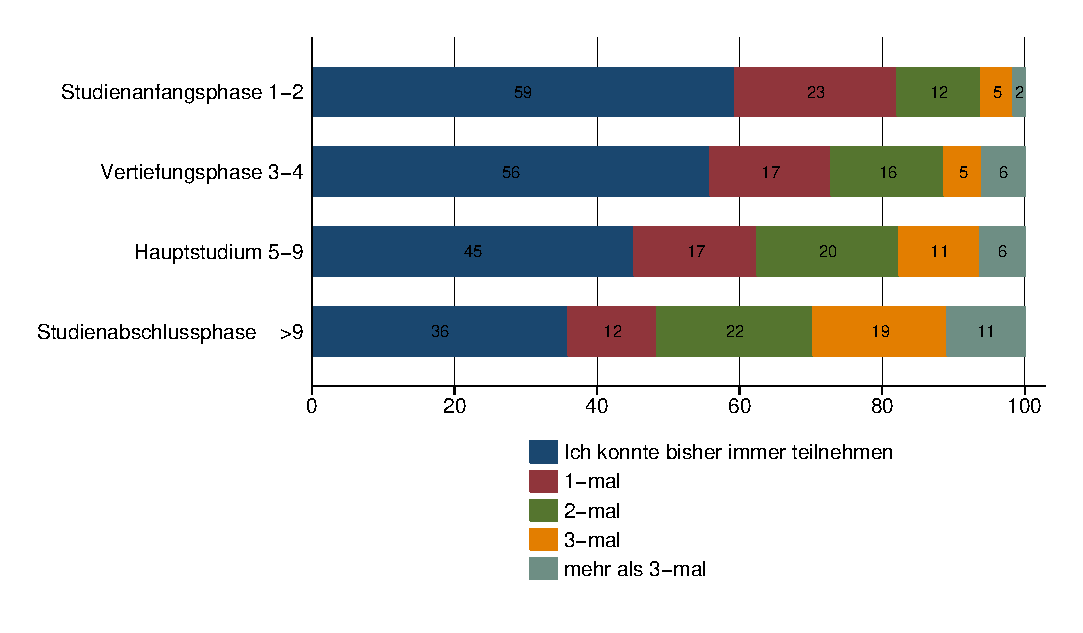
\includegraphics[
%  defaultresolution=72 !,
%  bmpsizefast=false
%]{image}
%\end{verbatim}
% \end{quote}
%
% \subsubsection{Hints}
%
% \begin{itemize}
% \item My version of \xfile{dvips.def} 1999/02/16 v3.0i defines
%       rules for the supported bitmap extensions, but does not
%       include them in the list of extensions that are tried
%       if the file name is not given with an extension.
%       In such a case, the list of extensions can be set
%       by \cs{DeclareGraphicsExtensions}, see \xpackage{grfguide}.
%       The following code just extends the list:
%       \begin{quote}
%\begin{verbatim}
%\makeatletter
%\g@addto@macro\Gin@extensions{,.bmp,.pcx,.msp}
%\makeatother
%\end{verbatim}
%       \end{quote}
% \item My version of \xfile{dvipdfm.def} 1998/11/24 vx.x misses
%       the graphics rule for PNG files. It can be added by:
%       \begin{quote}
%\begin{verbatim}
%\DeclareGraphicsRule{.png}{bmp}{.bb}{#1}
%\end{verbatim}
%       \end{quote}
%       See the previous issue to add the extension \xfile{.png} to the list
%       of extensions for package \xpackage{graphics}.
% \end{itemize}
%
% \subsubsection{Test program}
%
% There is a test program \xfile{bmpsize-test.tex}. Run it through
% \verb|latex|, \verb|pdflatex|, or \verb|pdftex|. Then given
% image files are inspected and the result is printed.
%
% \subsubsection{Interface for programmers}
%
% The macro names of the parsers are \verb|\bmpsize@read@|\meta{type}.
% Example: \cs{bmpsize@read@jpg} in case of JPEG.
%
% A parser sets the switch \cs{ifbmpsize@ok} to true, if it
% could successfully parse the image file.
% The width and height are returnd in \cs{bmpsize@width} and
% \cs{bmpsize@height}. If information about density is available,
% it is used to calculate width and height of the image, otherwise
% the values given by option \xoption{defaultresolution} is used.
% \xoption{resolution} overwrites the values in the image file.
%
% \subsection{Improved bitmap inclusion}
%
% Some drivers for package \xpackage{graphics} define the graphics
% type \xoption{bmp} for bitmap images. The code in the standard
% drivers for \xoption{dvips}, \xoption{dvipdfm}, and \xoption{dvipdfmx}
% is very basic and misses essential features of the
% package \xpackage{graphicx}. Therefore the code for bitmap
% inclusion is automatically rewritten by this package to add
% the following features:
% \begin{itemize}
% \item Support for \xoption{viewport} and \xoption{trim}.
% \item Support for \xoption{clip}.
% \item In case of \xoption{dvipdfm} and \xoption{dvipdfmx} the
%       bitmap images are reused and not included again if they
%       are used more than once.
% \end{itemize}
% However, there is a difference between \xoption{dvipdfm} and
% \xoption{dvipdfmx}, especially if images are reused. In the
% former case the reused box has width and height of 1bp, in the
% latter case its natural width. Thus the correct driver option must be given.
% \xoption{dvipdfm} and \xoption{dvipdfmx} are not equivalent.
%
% Older versions of \xoption{dvipdfmx} uses a size of 1in. However I do
% want to distinguish between versions of the same program. Therefore the
% support of these older versions has stopped with version 1.6 of this package.
% Use version dvipdfmx-20090708 or newer (some few versions before will
% probably also work, but I don't want to investigate this further).
%
% \StopEventually{
% }
%
% \section{Implementation}
%
% \subsection{Basic package \xpackage{bmpsize-base}}
%
%    Identification.
%    \begin{macrocode}
%<*base>
\ProvidesPackage{bmpsize-base}%
  [2009/09/04 v1.6 Basic part of bmpsize (HO)]%
%    \end{macrocode}
%    Modules of package \xpackage{fp} are used for calculations.
%    \begin{macrocode}
\RequirePackage{fp-basic}
\RequirePackage{fp-snap}
%    \end{macrocode}
%    Package \xpackage{fp} uses nested \cs{loop} structures.
%    That breaks with the plain-\TeX\ version of \cs{loop}.
%    Therefore we use the \LaTeX\ variant.
%    \begin{macro}{\@bmpsize@plain@loop}
%    \begin{macrocode}
\long\def\@bmpsize@plain@loop#1\repeat{%
  \def\iterate{%
    #1\relax
    \expandafter\iterate\fi
  }%
  \iterate
  \let\iterate\relax
}
%    \end{macrocode}
%    \end{macro}
%    \begin{macrocode}
\RequirePackage{pdftexcmds}[2007/11/11]
%    \end{macrocode}
%    \begin{macrocode}
\newif\ifbmpsize@ok
\let\@bmpsize@ok\bmpsize@oktrue

\newif\if@bmpsize@bigendian
\newif\if@bmpsize@absnum
\newif\if@bmpsize@user@resolution
\newif\if@bmpsize@fast
\@bmpsize@fasttrue

\def\@bmpsize@init{%
  \let\@bmpsize@org@plain@loop\loop
  \let\loop\@bmpsize@plain@loop
  \bmpsize@okfalse
  \@bmpsize@bigendiantrue
  \@bmpsize@absnumfalse
  \let\bmpsize@pixelwidth\relax
  \let\bmpsize@pixelheight\relax
  \let\bmpsize@pixelx\relax
  \let\bmpsize@pixely\relax
  \let\bmpsize@unit\relax
  \let\bmpsize@pixelxdenom\relax
  \let\bmpsize@pixelydenom\relax
  \let\bmpsize@orientation\relax
}

\def\@bmpsize@stop#1\@nil{}

\def\@bmpsize@loop#1{%
  #1%
  \@bmpsize@loop{#1}%
}
\def\@bmpsize@break#1\@bmpsize@loop#2{}

\def\@bmpsize@size#1#2#3{%
  \edef#3{\pdf@filesize{#1}}%
  \ifx#3\@empty
    \expandafter\@bmpsize@stop
  \fi
  \ifnum#3<#2\relax
    \expandafter\@bmpsize@stop
  \fi
}

\def\@bmpsize@read#1#2#3{%
  \edef\@bmpsize@buf{\pdf@filedump{#3}{#2}{#1}}%
  \edef\@bmpsize@temp{%
    \noexpand\@bmpsize@check@byte{#2}\@bmpsize@buf{}{}\noexpand\\%
  }%
  \@bmpsize@temp
}
\def\@bmpsize@fillbuf#1{%
  \ifx\@bmpsize@buf\@empty
    \expandafter\@firstofone
  \else
    \expandafter\@gobble
  \fi
  {%
    \edef\@bmpsize@buf{%
      \pdf@filedump{\bmpsize@offset}{\bmpsize@fillbuflength}{#1}%
    }%
    \ifx\@bmpsize@buf\@empty
      \expandafter\@bmpsize@stop
    \fi
    \edef\bmpsize@offset{\the\numexpr\bmpsize@offset+\bmpsize@fillbuflength}%
  }%
}
\def\bmpsize@fillbuflength{10}

\def\@bmpsize@append#1#2#3{%
  \edef#1{#2#3}%
}
\def\@bmpsize@pushback#1{%
  \edef\@bmpsize@buf{#1\@bmpsize@buf}%
}

\def\@bmpsize@iswhite#1{%
  \ifnum\pdf@strcmp{#1}{09}=\z@
  \else
    \ifnum\pdf@strcmp{#1}{0A}=\z@
    \else
      \ifnum\pdf@strcmp{#1}{0D}=\z@
      \else
        \ifnum\pdf@strcmp{#1}{20}=\z@
        \else
          1%
        \fi
      \fi
    \fi
  \fi
  \space
}
\def\@bmpsize@isdigit#1{%
  \ifnum\pdf@strcmp{#1}{30}<\z@
    1%
  \else
    \ifnum\pdf@strcmp{#1}{39}>\z@
      1%
    \fi
  \fi
  \space
}

\def\@bmpsize@check@byte#1#2#3{%
  \ifnum#1<\@ne
    \csname fi\endcsname
    \@bmpsize@cleanup@end
  \else
    \csname fi\endcsname
  \ifx!#2#3!%
    \csname fi\endcsname
    \@bmpsize@stop
  \else
    \csname fi\endcsname
    \expandafter\@bmpsize@check@byte\expandafter{\the\numexpr#1-1}%
}
\def\@bmpsize@cleanup@end#1\\{}

\def\@bmpsize@swap@maybe#1{%
  \if@bmpsize@bigendian
  \else
    \edef#1{\expandafter\@bmpsize@@swap#1\@empty\@empty\@empty\@empty}%
  \fi
}
\def\@bmpsize@@swap#1#2#3#4#5#6#7#8{%
  #7#8#5#6#3#4#1#2%
}

\def\@bmpsize@skip@one{%
  \edef\@bmpsize@buf{\expandafter\@gobbletwo\@bmpsize@buf}%
}
\def\@bmpsize@skip@two{%
  \edef\@bmpsize@buf{\expandafter\@gobblefour\@bmpsize@buf}%
}
\def\@bmpsize@skip@four{%
  \edef\@bmpsize@buf{%
    \expandafter\expandafter\expandafter\@gobblefour\expandafter
    \@gobblefour\@bmpsize@buf
  }%
}

\def\@bmpsize@grab#1#2{%
  \edef#1{\noexpand\@bmpsize@grab@byte#2=\@bmpsize@buf\noexpand\\}%
  \edef#1{#1}%
}
\def\@bmpsize@grab@byte#1=#2#3{%
  #2#3%
  \ifnum#1>\@ne
    \expandafter\@bmpsize@grab@byte\the\numexpr#1-1\expandafter=%
  \else
    \expandafter\@bmpsize@cleanup@end
  \fi
}

\def\@bmpsize@abs@maybe#1{%
  \let\@bmpsize@temp\relax
  \if@bmpsize@absnum
    \ifnum"\expandafter\@car#1\@nil>7 %
      \edef#1{\expandafter\@bmpsize@abs@byte#1\relax}%
      \ifnum\pdf@strcmp{#1}{7FFFFFFF}=\z@
        \let\@bmpsize@temp\@bmpsize@stop
      \else
        \def\@bmpsize@temp{\edef#1{\the\numexpr#1+1}}%
      \fi
    \fi
  \fi
}
\def\@bmpsize@abs@byte#1{%
  \ifx#1\relax
  \else
    \ifcase"0#1 %
      F\or E\or D\or C\or B\or A\or 9\or 8\or
      7\or 6\or 5\or 4\or 3\or 2\or 1\or 0%
    \fi
    \expandafter\@bmpsize@abs@byte
  \fi
}

\def\@bmpsize@num@one#1{%
  \@bmpsize@grab#11%
  \@bmpsize@abs@maybe#1%
  \edef#1{\number"#1}%
  \@bmpsize@temp
  \@bmpsize@skip@one
}
\def\@bmpsize@num@two#1{%
  \@bmpsize@grab#12%
  \@bmpsize@swap@maybe#1%
  \@bmpsize@abs@maybe#1%
  \edef#1{\number"#1}%
  \@bmpsize@temp
  \@bmpsize@skip@two
}
\def\@bmpsize@num@four#1{%
  \@bmpsize@grab#14%
  \@bmpsize@swap@maybe#1%
  \@bmpsize@abs@maybe#1%
  \ifnum\pdf@strcmp{#1}{7FFFFFFF}>\z@
    \expandafter\@bmpsize@stop
  \fi
  \edef#1{\number"#1}%
  \@bmpsize@temp
  \@bmpsize@skip@four
}

\def\@bmpsize@div#1#2#3{% #1 := #2/#3
  \FPdiv#1{#2}{#3}%
  \@bmpsize@beautify#1%
}
\def\@bmpsize@beautify#1{%
  \FPifint#1%
    \edef#1{\expandafter\@bmpsize@trunc#1.\@nil}%
  \else
    \edef#1{\expandafter\@bmpsize@cleanup@frac#1.\@nil}%
  \fi
}
\def\@bmpsize@trunc#1.#2\@nil{#1}
% #1 isn't an integer, thus we should have at least one
% necessary digit after the dot
\def\@bmpsize@cleanup@frac#1.#2#3.#4\@nil{%
  #1.#2%
  \ifx\\#3\\%
  \else
    \@bmpsize@cleanup@fracdigits#3000000000\@nil
  \fi
}
\def\@bmpsize@cleanup@fracdigits#1#2#3#4#5#6#7#8#9{%
  \ifcase#9 %
    \ifcase#8 %
      \ifcase#7 %
        \ifcase#6 %
          \ifcase#5 %
            \ifcase #4 %
              \ifcase #3 %
                \ifcase #2 %
                  \ifcase #1 %
                  \else
                    #1%
                  \fi
                \else
                  #1#2%
                \fi
              \else
                #1#2#3%
              \fi
            \else
              #1#2#3#4%
            \fi
          \else
            #1#2#3#4#5%
          \fi
        \else
          #1#2#3#4#5#6%
        \fi
      \else
        #1#2#3#4#5#6#7%
      \fi
    \else
      #1#2#3#4#5#6#7#8%
    \fi
  \else
    #1#2#3#4#5#6#7#8#9%
  \fi
  \@bmpsize@trunc.%
}

\def\@bmpsize@end{%
  \ifbmpsize@ok
    \ifx\bmpsize@pixelwidth\relax
      \bmpsize@okfalse
    \fi
    \ifx\bmpsize@pixelheight\relax
      \bmpsize@okfalse
    \fi
  \fi
  \ifbmpsize@ok
    \ifnum\bmpsize@pixelwidth>\z@
    \else
      \bmpsize@okfalse
    \fi
    \ifnum\bmpsize@pixelheight>\z@
    \else
      \bmpsize@okfalse
    \fi
  \fi
  \ifbmpsize@ok
    \ifcase 0%
      \ifx\bmpsize@pixelx\relax 1 \fi
      \ifx\bmpsize@pixely\relax 1 \fi
      \ifnum\bmpsize@pixelx>\z@\else 1 \fi
      \ifnum\bmpsize@pixely>\z@\else 1 \fi
      \ifx\bmpsize@pixelxdenom\relax
         \ifx\bmpsize@pixelydenom\relax\else 1 \fi
      \else
        \ifnum\bmpsize@pixelxdenom>\z@\else 1 \fi
      \fi
      \ifx\bmpsize@pixelydenom\relax
      \else
        \ifnum\bmpsize@pixelydenom>\z@\else 1 \fi
      \fi
    \else
      \let\bmpsize@pixelx\relax
      \let\bmpsize@pixely\relax
      \let\bmpsize@unit\relax
      \let\bmpsize@pixelxdenom\relax
      \let\bmpsize@pixelydenom\relax
    \fi
    \ifx\bmpsize@pixelxdenom\relax
    \else
      \@bmpsize@div\bmpsize@pixelx\bmpsize@pixelx\bmpsize@pixelxdenom
      \@bmpsize@div\bmpsize@pixely\bmpsize@pixely\bmpsize@pixelydenom
      \let\bmpsize@pixelxdenom\relax
      \let\bmpsize@pixelydenom\relax
    \fi
    \ifcase 0\ifx\bmpsize@unit\relax 1\fi
             \if@bmpsize@user@resolution 1\fi
             \relax
      \let\bmpsize@calc@unit\bmpsize@unit
      \let\bmpsize@calc@pixelx\bmpsize@pixelx
      \let\bmpsize@calc@pixely\bmpsize@pixely
    \else
      \let\bmpsize@calc@unit\bmpsize@unit@default
      \let\bmpsize@calc@pixelx\bmpsize@pixelx@default
      \let\bmpsize@calc@pixely\bmpsize@pixely@default
      \ifx\bmpsize@calc@pixely\Gin@exclamation
        \ifx\bmpsize@pixelx\relax
          \let\bmpsize@calc@pixely\bmpsize@calc@pixelx
        \else
          \FPdiv\bmpsize@calc@pixely\bmpsize@calc@pixelx\bmpsize@pixelx
          \FPmul\bmpsize@calc@pixely\bmpsize@calc@pixely\bmpsize@pixely
        \fi
      \else
        \ifx\bmpsize@calc@pixelx\Gin@exclamation
          \ifx\bmpsize@pixelx\relax
            \let\bmpsize@calc@pixelx\bmpsize@calc@pixely
          \else
            \FPdiv\bmpsize@calc@pixelx\bmpsize@calc@pixely\bmpsize@pixely
            \FPmul\bmpsize@calc@pixelx\bmpsize@calc@pixelx\bmpsize@pixelx
          \fi
        \fi
      \fi
    \fi
    \FPdiv\bmpsize@width\bmpsize@pixelwidth\bmpsize@calc@pixelx
    \FPdiv\bmpsize@height\bmpsize@pixelheight\bmpsize@calc@pixely
    % calculation of width and height in bp for package graphics
    % 1in = 72bp = 72.27pt, 72/72.27 = 8/8.03, 1pt = 65536sp
    \if@bmpsize@fast
      \edef\bmpsize@width{%
        \strip@pt\dimexpr.99626\dimexpr
        \bmpsize@width\dimexpr\bmpsize@calc@unit
      }%
      \edef\bmpsize@height{%
        \strip@pt\dimexpr.99626\dimexpr
        \bmpsize@height\dimexpr\bmpsize@calc@unit
      }%
    \else
      \edef\@bmpsize@temp{\number\dimexpr\bmpsize@calc@unit}%
      \ifnum\@bmpsize@temp>100000 %
        \FPmul\@bmpsize@temp\@bmpsize@temp{0.00001}%
        \def\@bmpsize@corr{100000}%
      \else
        \let\@bmpsize@corr\relax
      \fi
      \FPmul\bmpsize@width\bmpsize@width\@bmpsize@temp
      \FPmul\bmpsize@height\bmpsize@height\@bmpsize@temp
      \FPmul\bmpsize@width\bmpsize@width{8}%
      \FPmul\bmpsize@height\bmpsize@height{8}%
      \FPdiv\bmpsize@width\bmpsize@width{8.03}%
      \FPdiv\bmpsize@height\bmpsize@height{8.03}%
      \FPdiv\bmpsize@width\bmpsize@width{65536}%
      \FPdiv\bmpsize@height\bmpsize@height{65536}%
      \ifx\@bmpsize@corr\relax
      \else
        \FPmul\bmpsize@width\bmpsize@width\@bmpsize@corr
        \FPmul\bmpsize@height\bmpsize@height\@bmpsize@corr
      \fi
      \FPround\bmpsize@width\bmpsize@width{5}%
      \FPround\bmpsize@height\bmpsize@height{5}%
      \@bmpsize@beautify\bmpsize@width
      \@bmpsize@beautify\bmpsize@height
    \fi
  \fi
  \let\loop\@bmpsize@org@plain@loop
}
\def\bmpsize@unit@default{72.27pt}% more accurate than 1in
\def\bmpsize@pixelx@default{72}
\let\bmpsize@pixely@default\Gin@exclamation

\def\bmpsize@types{png,jpg,bmp,gif,tiff,pnm,pam,xpm,tga,pcx,msp,sgi}
%</base>
%    \end{macrocode}
%
% \subsection{Bitmap formats}
%
% \subsubsection{png}
%
%\iffalse
%<*ignore>
%\fi
%\begin{verbatim}
%begin png
%big-endian
%
%read 24 0
%grab 8        -> $temp
%check streq $temp [0x89 "PNG" 0x0D 0x0A 0x1A 0x0A]
%num 4         -> $length
%grab 4        -> $temp
%check streq $temp ["IHDR"]
%num 4         -> $pixelwidth
%num 4         -> $pixelheight
%ok
%assign numexpr(20 + $length) -> $offset
%loop
%  read 8 $offset
%  num 4       -> $length
%  grab 4      -> $temp
%  if streq $temp ["IDAT"]
%    stop
%  fi
%  if streq $temp ["pHYs"]
%    read 9 numexpr($offset + 8)
%    num 4     -> $pixelx
%    num 4     -> $pixely
%    grab 1     -> $temp
%    if numeq $temp 1
%      assign {100cm} -> $unit
%    fi
%    stop
%  fi
%  assign numexpr($offset + 12 + $length) -> $offset
%repeat
%end
%\end{verbatim}
%\iffalse
%</ignore>
%\fi
%    \begin{macro}{\bmpsize@read@png}
%    \begin{macrocode}
%<*base>
\def\bmpsize@read@png#1{%
  \@bmpsize@init
  \@bmpsize@bigendiantrue
  \@bmpsize@read{#1}{24}{0}%
  \@bmpsize@grab\bmpsize@temp{8}%
  \@bmpsize@skip@four
  \@bmpsize@skip@four
  \ifnum\pdf@strcmp{\bmpsize@temp}{89504E470D0A1A0A}=\z@
  \else
    \expandafter\@bmpsize@stop
  \fi
  \@bmpsize@num@four\bmpsize@length
  \@bmpsize@grab\bmpsize@temp{4}%
  \@bmpsize@skip@four
  \ifnum\pdf@strcmp{\bmpsize@temp}{49484452}=\z@
  \else
    \expandafter\@bmpsize@stop
  \fi
  \@bmpsize@num@four\bmpsize@pixelwidth
  \@bmpsize@num@four\bmpsize@pixelheight
  \@bmpsize@ok
  \edef\bmpsize@offset{\the\numexpr20+\bmpsize@length}%
  \@bmpsize@loop{%
    \@bmpsize@read{#1}{8}{\bmpsize@offset}%
    \@bmpsize@num@four\bmpsize@length
    \@bmpsize@grab\bmpsize@temp{4}%
    \@bmpsize@skip@four
    \ifnum\pdf@strcmp{\bmpsize@temp}{49444154}=\z@
      \expandafter\@firstofone
    \else
      \expandafter\@gobble
    \fi
    {%
      \@bmpsize@stop
    }%
    \ifnum\pdf@strcmp{\bmpsize@temp}{70485973}=\z@
      \expandafter\@firstofone
    \else
      \expandafter\@gobble
    \fi
    {%
      \@bmpsize@read{#1}{9}{\numexpr\bmpsize@offset+8\relax}%
      \@bmpsize@num@four\bmpsize@pixelx
      \@bmpsize@num@four\bmpsize@pixely
      \@bmpsize@grab\bmpsize@temp{1}%
      \@bmpsize@skip@one
      \ifnum\bmpsize@temp=1\relax
        \expandafter\@firstofone
      \else
        \expandafter\@gobble
      \fi
      {%
        \def\bmpsize@unit{100cm}%
      }%
      \@bmpsize@stop
    }%
    \edef\bmpsize@offset{\the\numexpr\bmpsize@offset+12+\bmpsize@length}%
  }%
  \@bmpsize@stop
  \@nil
  \@bmpsize@end
}%
%</base>
%    \end{macrocode}
%    \end{macro}
%
% \subsubsection{jpg}
%
%\iffalse
%<*ignore>
%\fi
%\begin{verbatim}
%begin jpg
%
%read 3 0
%grab 3      -> $temp % SOI and 0xFF
%check streq $temp [0xFF 0xD8 0xFF]
%assign {2} -> $offset
%assign {0} -> $exifdensity
%loop
%  read 4 $offset
%  grab 1    -> $temp
%  check streq $temp [0xFF]
%  num 1    -> $temp
%  if numeq $temp 0xDA % SOS
%    stop
%  fi
%  % look for JFIF APP0 segment
%  if numeq $temp 0xE0 % APP0
%    num 2       -> $length
%    if numeq $exifdensity 0
%      if numge $length 16 % a JFIF segment has 16 bytes at least
%        read 12 numexpr($offset + 4)
%        grab 5      -> $temp % identifier
%        if streq $temp ["JFIF" 0x0]
%          check numge $length 16
%          skip 2 % version
%          num 1       -> $temp % units
%          if numeq $temp 1
%            assign {72.27pt} -> $unit
%          else
%            if numeq $temp 2
%              assign {1cm} -> $unit
%            fi
%          fi
%          num 2    -> $pixelx
%          num 2    -> $pixely
%        fi
%      fi
%    fi
%  else
%    if numeq $temp 0xE1 % APP1
%      % look for Exif APP1 segment
%      num 2 -> $length
%      if numge $length 20 % identifier (6) + Tiff header (8) + first IFD (>=6)
%        read 20 numexpr($offset + 4)
%        grab 6 -> $temp
%        if streq $temp ["Exif" 0x0 0x0]
%          assign numexpr($offset + 10) -> $exifoffset
%          % read TIFF header
%          grab 2 -> $temp
%          if streq $temp ["II"]
%            little-endian
%          else
%            check streq $temp ["MM"]
%            % big-endian
%          fi
%          num 2 -> $temp
%          check numeq $temp 42
%          num 4 -> $temp % offset of first IFD
%          check numgt $temp 0
%          % read first IFD
%          assign numexpr($temp + $exifoffset) -> $off
%          read 2 $off
%          num 2 -> $entries
%          assign numexpr($off + 2) -> $off
%          loop
%            if numeq $entries 0
%              break
%            fi
%            assign numexpr($entries - 1) -> $entries
%            % entry format:
%            % 2 tag
%            % 2 field type
%            % 4 count
%            % 4 value/offset
%            read 12 $off
%            assign numexpr($off + 12) -> $off
%            num 2 -> $tag
%            if numeq $tag 296 % ResolutionUnit
%              skip 6 % type: 3 (short), count: 1
%              num 2 -> $temp
%              ifcase $temp
%              or % 1
%                clear $unit
%              or % 2
%                assign {72.27pt} -> $unit
%              or % 3
%                assign {1cm} -> $unit
%              else
%                clear $unit % unknown
%              fi
%              ifcase $temp
%              or % 1
%              or % 2
%                assign {1} -> $exifdensity
%              or % 3
%                assign {1} -> $exifdensity
%              else
%                assign $exifdensity -> $exifdensity
%              fi
%            fi
%            % 256 ImageWidth (use width of JPG part)
%            % 257 ImageHeight (use height of JPG part)
%            if numeq $tag 274 % Orientation
%              skip 6 % type: 3 (short), count: 1
%              num 2 -> $temp
%              if numge $temp 0 
%                if numle $temp 8
%                  assign $temp -> $orientation
%                fi
%              fi
%            fi
%            if numeq $tag 282 % XResolution
%              skip 6
%              num 4 -> $temp
%              read 8 numexpr($temp + $exifoffset)
%              num 4 -> $pixelx
%              num 4 -> $temp
%              if numeq $temp 1
%              else
%                assign numexpr($temp) -> $pixelxdenom
%                % div $pixelx $temp -> $pixelx
%              fi
%            fi
%            if numeq $tag 283 % YResolution
%              skip 6
%              num 4 -> $temp
%              read 8 numexpr($temp + $exifoffset)
%              num 4 -> $pixely
%              num 4 -> $temp
%              if numeq $temp 1
%              else
%                assign numexpr($temp) -> $pixelydenom
%                % div $pixely $temp -> $pixely
%              fi
%            fi
%          repeat
%          big-endian
%        fi
%      fi
%    else
%      assign numexpr($temp - 0xC0) -> $temp
%      ifcase $temp % SOF_0
%      or % SOF_1
%      or % SOF_2
%      or % SOF_3
%      or % DHT
%        assign {-1} -> $temp
%      or % SOF_5
%      or % SOF_6
%      or % SOF_7
%      or % JPG
%        assign {-1} -> $temp
%      or % SOF_9
%      or % SOF_10
%      or % SOF_11
%      or % DAC
%        assign {-1} -> $temp
%      or % SOF_13
%      or % SOF_14
%      or % SOF_15
%      else
%        assign {-1} -> $temp
%      fi
%      if numeq $temp -1
%      else
%        read 4 numexpr($offset + 5)
%        num 2  -> $pixelheight
%        num 2  -> $pixelwidth
%        if numeq $pixelheight 0
%          clear $pixelheight
%          stop
%        fi
%        ok
%        stop
%      fi
%      num 2 -> $length
%    fi
%  fi
%  assign numexpr($offset + $length + 2) -> $offset
%repeat
%end
%\end{verbatim}
%\iffalse
%</ignore>
%\fi
%    \begin{macro}{\bmpsize@read@jpg}
%    \begin{macrocode}
%<*base>
\def\bmpsize@read@jpg#1{%
  \@bmpsize@init
  \@bmpsize@read{#1}{3}{0}%
  \@bmpsize@grab\bmpsize@temp{3}%
  \@bmpsize@skip@two
  \@bmpsize@skip@one
  \ifnum\pdf@strcmp{\bmpsize@temp}{FFD8FF}=\z@
  \else
    \expandafter\@bmpsize@stop
  \fi
  \def\bmpsize@offset{2}%
  \def\bmpsize@exifdensity{0}%
  \@bmpsize@loop{%
    \@bmpsize@read{#1}{4}{\bmpsize@offset}%
    \@bmpsize@grab\bmpsize@temp{1}%
    \@bmpsize@skip@one
    \ifnum\pdf@strcmp{\bmpsize@temp}{FF}=\z@
    \else
      \expandafter\@bmpsize@stop
    \fi
    \@bmpsize@num@one\bmpsize@temp
    \ifnum\bmpsize@temp=218\relax
      \expandafter\@firstofone
    \else
      \expandafter\@gobble
    \fi
    {%
      \@bmpsize@stop
    }%
    \ifnum\bmpsize@temp=224\relax
      \expandafter\@firstoftwo
    \else
      \expandafter\@secondoftwo
    \fi
    {%
      \@bmpsize@num@two\bmpsize@length
      \ifnum\bmpsize@exifdensity=0\relax
        \expandafter\@firstofone
      \else
        \expandafter\@gobble
      \fi
      {%
        \unless\ifnum\bmpsize@length<16\relax
          \expandafter\@firstofone
        \else
          \expandafter\@gobble
        \fi
        {%
          \@bmpsize@read{#1}{12}{\numexpr\bmpsize@offset+4\relax}%
          \@bmpsize@grab\bmpsize@temp{5}%
          \@bmpsize@skip@four
          \@bmpsize@skip@one
          \ifnum\pdf@strcmp{\bmpsize@temp}{4A46494600}=\z@
            \expandafter\@firstofone
          \else
            \expandafter\@gobble
          \fi
          {%
            \ifnum\bmpsize@length<16\relax
              \expandafter\@bmpsize@stop
            \fi
            \@bmpsize@skip@two
            \@bmpsize@num@one\bmpsize@temp
            \ifnum\bmpsize@temp=1\relax
              \expandafter\@firstoftwo
            \else
              \expandafter\@secondoftwo
            \fi
            {%
              \def\bmpsize@unit{72.27pt}%
            }{%
              \ifnum\bmpsize@temp=2\relax
                \expandafter\@firstofone
              \else
                \expandafter\@gobble
              \fi
              {%
                \def\bmpsize@unit{1cm}%
              }%
            }%
            \@bmpsize@num@two\bmpsize@pixelx
            \@bmpsize@num@two\bmpsize@pixely
          }%
        }%
      }%
    }{%
      \ifnum\bmpsize@temp=225\relax
        \expandafter\@firstoftwo
      \else
        \expandafter\@secondoftwo
      \fi
      {%
        \@bmpsize@num@two\bmpsize@length
        \unless\ifnum\bmpsize@length<20\relax
          \expandafter\@firstofone
        \else
          \expandafter\@gobble
        \fi
        {%
          \@bmpsize@read{#1}{20}{\numexpr\bmpsize@offset+4\relax}%
          \@bmpsize@grab\bmpsize@temp{6}%
          \@bmpsize@skip@four
          \@bmpsize@skip@two
          \ifnum\pdf@strcmp{\bmpsize@temp}{457869660000}=\z@
            \expandafter\@firstofone
          \else
            \expandafter\@gobble
          \fi
          {%
            \edef\bmpsize@exifoffset{\the\numexpr\bmpsize@offset+10}%
            \@bmpsize@grab\bmpsize@temp{2}%
            \@bmpsize@skip@two
            \ifnum\pdf@strcmp{\bmpsize@temp}{4949}=\z@
              \expandafter\@firstoftwo
            \else
              \expandafter\@secondoftwo
            \fi
            {%
              \@bmpsize@bigendianfalse
            }{%
              \ifnum\pdf@strcmp{\bmpsize@temp}{4D4D}=\z@
              \else
                \expandafter\@bmpsize@stop
              \fi
            }%
            \@bmpsize@num@two\bmpsize@temp
            \ifnum\bmpsize@temp=42\relax
            \else
              \expandafter\@bmpsize@stop
            \fi
            \@bmpsize@num@four\bmpsize@temp
            \ifnum\bmpsize@temp>0\relax
            \else
              \expandafter\@bmpsize@stop
            \fi
            \edef\bmpsize@off{\the\numexpr\bmpsize@temp+\bmpsize@exifoffset}%
            \@bmpsize@read{#1}{2}{\bmpsize@off}%
            \@bmpsize@num@two\bmpsize@entries
            \edef\bmpsize@off{\the\numexpr\bmpsize@off+2}%
            \@bmpsize@loop{%
              \ifnum\bmpsize@entries=0\relax
                \expandafter\@firstofone
              \else
                \expandafter\@gobble
              \fi
              {%
                \@bmpsize@break
              }%
              \edef\bmpsize@entries{\the\numexpr\bmpsize@entries-1}%
              \@bmpsize@read{#1}{12}{\bmpsize@off}%
              \edef\bmpsize@off{\the\numexpr\bmpsize@off+12}%
              \@bmpsize@num@two\bmpsize@tag
              \ifnum\bmpsize@tag=296\relax
                \expandafter\@firstofone
              \else
                \expandafter\@gobble
              \fi
              {%
                \@bmpsize@skip@four
                \@bmpsize@skip@two
                \@bmpsize@num@two\bmpsize@temp
                \ifcase\bmpsize@temp\relax
                \or
                  \let\bmpsize@unit\relax
                \or
                  \def\bmpsize@unit{72.27pt}%
                \or
                  \def\bmpsize@unit{1cm}%
                \else
                  \let\bmpsize@unit\relax
                \fi
                \ifcase\bmpsize@temp\relax
                \or
                \or
                  \def\bmpsize@exifdensity{1}%
                \or
                  \def\bmpsize@exifdensity{1}%
                \else
                  \let\bmpsize@exifdensity\bmpsize@exifdensity
                \fi
              }%
              \ifnum\bmpsize@tag=274\relax
                \expandafter\@firstofone
              \else
                \expandafter\@gobble
              \fi
              {%
                \@bmpsize@skip@four
                \@bmpsize@skip@two
                \@bmpsize@num@two\bmpsize@temp
                \unless\ifnum\bmpsize@temp<0\relax
                  \expandafter\@firstofone
                \else
                  \expandafter\@gobble
                \fi
                {%
                  \unless\ifnum\bmpsize@temp>8\relax
                    \expandafter\@firstofone
                  \else
                    \expandafter\@gobble
                  \fi
                  {%
                    \let\bmpsize@orientation\bmpsize@temp
                  }%
                }%
              }%
              \ifnum\bmpsize@tag=282\relax
                \expandafter\@firstofone
              \else
                \expandafter\@gobble
              \fi
              {%
                \@bmpsize@skip@four
                \@bmpsize@skip@two
                \@bmpsize@num@four\bmpsize@temp
                \@bmpsize@read{#1}{8}{\numexpr\bmpsize@temp+\bmpsize@exifoffset\relax}%
                \@bmpsize@num@four\bmpsize@pixelx
                \@bmpsize@num@four\bmpsize@temp
                \ifnum\bmpsize@temp=1\relax
                  \expandafter\@gobble
                \else
                  \expandafter\@firstofone
                \fi
                {%
                  \edef\bmpsize@pixelxdenom{\the\numexpr\bmpsize@temp}%
                }%
              }%
              \ifnum\bmpsize@tag=283\relax
                \expandafter\@firstofone
              \else
                \expandafter\@gobble
              \fi
              {%
                \@bmpsize@skip@four
                \@bmpsize@skip@two
                \@bmpsize@num@four\bmpsize@temp
                \@bmpsize@read{#1}{8}{\numexpr\bmpsize@temp+\bmpsize@exifoffset\relax}%
                \@bmpsize@num@four\bmpsize@pixely
                \@bmpsize@num@four\bmpsize@temp
                \ifnum\bmpsize@temp=1\relax
                  \expandafter\@gobble
                \else
                  \expandafter\@firstofone
                \fi
                {%
                  \edef\bmpsize@pixelydenom{\the\numexpr\bmpsize@temp}%
                }%
              }%
            }%
            \@bmpsize@bigendiantrue
          }%
        }%
      }{%
        \edef\bmpsize@temp{\the\numexpr\bmpsize@temp-192}%
        \ifcase\bmpsize@temp\relax
        \or
        \or
        \or
        \or
          \def\bmpsize@temp{-1}%
        \or
        \or
        \or
        \or
          \def\bmpsize@temp{-1}%
        \or
        \or
        \or
        \or
          \def\bmpsize@temp{-1}%
        \or
        \or
        \or
        \else
          \def\bmpsize@temp{-1}%
        \fi
        \ifnum\bmpsize@temp=-1\relax
          \expandafter\@gobble
        \else
          \expandafter\@firstofone
        \fi
        {%
          \@bmpsize@read{#1}{4}{\numexpr\bmpsize@offset+5\relax}%
          \@bmpsize@num@two\bmpsize@pixelheight
          \@bmpsize@num@two\bmpsize@pixelwidth
          \ifnum\bmpsize@pixelheight=0\relax
            \expandafter\@firstofone
          \else
            \expandafter\@gobble
          \fi
          {%
            \let\bmpsize@pixelheight\relax
            \@bmpsize@stop
          }%
          \@bmpsize@ok
          \@bmpsize@stop
        }%
        \@bmpsize@num@two\bmpsize@length
      }%
    }%
    \edef\bmpsize@offset{\the\numexpr\bmpsize@offset+\bmpsize@length+2}%
  }%
  \@bmpsize@stop
  \@nil
  \@bmpsize@end
}%
%</base>
%    \end{macrocode}
%    \end{macro}
%
% \subsubsection{bmp}
%
%\iffalse
%<*ignore>
%\fi
%\begin{verbatim}
%begin bmp
%little-endian
%
%read 26 0
%grab 2 -> $temp
%check streq $temp ["BM"]
%skip 12
%% header size is 4 bytes in V3+, unknown for V1, V2,
%% known header sizes fit in 2 bytes
%num 2   -> $temp
%if numeq $temp 12 % V1
%  skip 2
%  num 2 -> $pixelwidth
%  num 2 -> $pixelheight
%  % no resolution entries
%  ok
%  stop
%fi
%if numeq $temp 64 % V2
%  skip 2
%  num 2 -> $pixelwidth
%  num 2 -> $pixelheight
%  % missing specification for resolution
%  ok
%  stop
%fi
%% V3, V4, V5
%skip 2
%num 4 -> $pixelwidth
%absnum 4 -> $pixelheight
%ok
%read 8 38
%num 4 -> $pixelx
%num 4 -> $pixely
%assign {100cm} -> $unit
%end
%\end{verbatim}
%\iffalse
%</ignore>
%\fi
%    \begin{macro}{\bmpsize@read@bmp}
%    \begin{macrocode}
%<*base>
\def\bmpsize@read@bmp#1{%
  \@bmpsize@init
  \@bmpsize@bigendianfalse
  \@bmpsize@read{#1}{26}{0}%
  \@bmpsize@grab\bmpsize@temp{2}%
  \@bmpsize@skip@two
  \ifnum\pdf@strcmp{\bmpsize@temp}{424D}=\z@
  \else
    \expandafter\@bmpsize@stop
  \fi
  \@bmpsize@skip@four
  \@bmpsize@skip@four
  \@bmpsize@skip@four
  \@bmpsize@num@two\bmpsize@temp
  \ifnum\bmpsize@temp=12\relax
    \expandafter\@firstofone
  \else
    \expandafter\@gobble
  \fi
  {%
    \@bmpsize@skip@two
    \@bmpsize@num@two\bmpsize@pixelwidth
    \@bmpsize@num@two\bmpsize@pixelheight
    \@bmpsize@ok
    \@bmpsize@stop
  }%
  \ifnum\bmpsize@temp=64\relax
    \expandafter\@firstofone
  \else
    \expandafter\@gobble
  \fi
  {%
    \@bmpsize@skip@two
    \@bmpsize@num@two\bmpsize@pixelwidth
    \@bmpsize@num@two\bmpsize@pixelheight
    \@bmpsize@ok
    \@bmpsize@stop
  }%
  \@bmpsize@skip@two
  \@bmpsize@num@four\bmpsize@pixelwidth
  \@bmpsize@absnumtrue
  \@bmpsize@num@four\bmpsize@pixelheight
  \@bmpsize@absnumfalse
  \@bmpsize@ok
  \@bmpsize@read{#1}{8}{38}%
  \@bmpsize@num@four\bmpsize@pixelx
  \@bmpsize@num@four\bmpsize@pixely
  \def\bmpsize@unit{100cm}%
  \@bmpsize@stop
  \@nil
  \@bmpsize@end
}%
%</base>
%    \end{macrocode}
%    \end{macro}
%
% \subsubsection{gif}
%
%\iffalse
%<*ignore>
%\fi
%\begin{verbatim}
%begin gif
%little-endian
%
%% Header
%read 13 0
%grab 3      -> $temp
%check streq $temp ["GIF"]
%skip 3      % version
%
%% Logical Screen Descriptor
%num 2       -> $pixelwidth
%num 2       -> $pixelheight
%skip 2
%num 1       -> $temp % Pixel Aspect Ratio
%if numeq $temp 0
%else
%  assign numexpr($temp + 15) -> $pixelx
%  assign {64}     -> $pixely
%fi
%ok
%end
%\end{verbatim}
%\iffalse
%</ignore>
%\fi
%    \begin{macro}{\bmpsize@read@gif}
%    \begin{macrocode}
%<*base>
\def\bmpsize@read@gif#1{%
  \@bmpsize@init
  \@bmpsize@bigendianfalse
  \@bmpsize@read{#1}{13}{0}%
  \@bmpsize@grab\bmpsize@temp{3}%
  \@bmpsize@skip@two
  \@bmpsize@skip@one
  \ifnum\pdf@strcmp{\bmpsize@temp}{474946}=\z@
  \else
    \expandafter\@bmpsize@stop
  \fi
  \@bmpsize@skip@two
  \@bmpsize@skip@one
  \@bmpsize@num@two\bmpsize@pixelwidth
  \@bmpsize@num@two\bmpsize@pixelheight
  \@bmpsize@skip@two
  \@bmpsize@num@one\bmpsize@temp
  \ifnum\bmpsize@temp=0\relax
    \expandafter\@gobble
  \else
    \expandafter\@firstofone
  \fi
  {%
    \edef\bmpsize@pixelx{\the\numexpr\bmpsize@temp+15}%
    \def\bmpsize@pixely{64}%
  }%
  \@bmpsize@ok
  \@bmpsize@stop
  \@nil
  \@bmpsize@end
}%
%</base>
%    \end{macrocode}
%    \end{macro}
%
% \subsubsection{tiff}
%
%\iffalse
%<*ignore>
%\fi
%\begin{verbatim}
%begin tiff
%% defaults
%assign {72.27pt} -> $unit
%
%% Image File Header
%read 8 0
%grab 2 -> $temp
%if streq $temp ["II"]
%  little-endian
%else
%  check streq $temp ["MM"]
%  big-endian
%fi
%num 2 -> $temp
%check numeq $temp 42
%num 4 -> $offset % first IFD (Image File Directory)
%
%% First IFD
%read 2 $offset
%assign numexpr($offset + 2) -> $offset
%num 2 -> $entries
%ok % must rely on checks at the end
%loop
%  if numeq $entries 0
%    stop
%  fi
%  assign numexpr($entries - 1) -> $entries
%  % entry format:
%  % 2 tag
%  % 2 field type
%  % 4 count
%  % 4 value/offset
%  read 12 $offset
%  assign numexpr($offset + 12) -> $offset
%  num 2 -> $tag % tag
%  if numeq $temp 296 % ResolutionUnit
%    skip 6 % type: 3 (short), count: 1
%    num 2 -> $temp
%    ifcase $temp
%    or % 1
%      clear $unit
%    or % 2
%      assign {72.27pt} -> $unit
%    or % 3
%      assign {1cm} -> $unit
%    else
%      clear $unit
%    fi
%  fi
%  if numeq $tag 256 % ImageWidth
%    skip 6
%    num 4 -> $pixelwidth
%  fi
%  if numeq $tag 257 % ImageLength
%    skip 6
%    num 4 -> $pixelheight
%  fi
%  if numeq $tag 282 % XResolution
%    skip 6
%    num 4 -> $temp
%    read 8 $temp
%    num 4 -> $pixelx
%    num 4 -> $temp
%    if numeq $temp 1
%    else
%      assign numexpr($temp) -> $pixelxdenom
%      % div $pixelx $temp -> $pixelx
%    fi
%  fi
%  if numeq $tag 283 % YResolution
%    skip 6
%    num 4 -> $temp
%    read 8 $temp
%    num 4 -> $pixely
%    num 4 -> $temp
%    if numeq $temp 1
%    else
%      assign numexpr($temp) -> $pixelydenom
%      % div $pixely $temp -> $pixely
%    fi
%  fi
%repeat
%end
%\end{verbatim}
%\iffalse
%</ignore>
%\fi
%    \begin{macro}{\bmpsize@read@tiff}
%    \begin{macrocode}
%<*base>
\def\bmpsize@read@tiff#1{%
  \@bmpsize@init
  \def\bmpsize@unit{72.27pt}%
  \@bmpsize@read{#1}{8}{0}%
  \@bmpsize@grab\bmpsize@temp{2}%
  \@bmpsize@skip@two
  \ifnum\pdf@strcmp{\bmpsize@temp}{4949}=\z@
    \expandafter\@firstoftwo
  \else
    \expandafter\@secondoftwo
  \fi
  {%
    \@bmpsize@bigendianfalse
  }{%
    \ifnum\pdf@strcmp{\bmpsize@temp}{4D4D}=\z@
    \else
      \expandafter\@bmpsize@stop
    \fi
    \@bmpsize@bigendiantrue
  }%
  \@bmpsize@num@two\bmpsize@temp
  \ifnum\bmpsize@temp=42\relax
  \else
    \expandafter\@bmpsize@stop
  \fi
  \@bmpsize@num@four\bmpsize@offset
  \@bmpsize@read{#1}{2}{\bmpsize@offset}%
  \edef\bmpsize@offset{\the\numexpr\bmpsize@offset+2}%
  \@bmpsize@num@two\bmpsize@entries
  \@bmpsize@ok
  \@bmpsize@loop{%
    \ifnum\bmpsize@entries=0\relax
      \expandafter\@firstofone
    \else
      \expandafter\@gobble
    \fi
    {%
      \@bmpsize@stop
    }%
    \edef\bmpsize@entries{\the\numexpr\bmpsize@entries-1}%
    \@bmpsize@read{#1}{12}{\bmpsize@offset}%
    \edef\bmpsize@offset{\the\numexpr\bmpsize@offset+12}%
    \@bmpsize@num@two\bmpsize@tag
    \ifnum\bmpsize@temp=296\relax
      \expandafter\@firstofone
    \else
      \expandafter\@gobble
    \fi
    {%
      \@bmpsize@skip@four
      \@bmpsize@skip@two
      \@bmpsize@num@two\bmpsize@temp
      \ifcase\bmpsize@temp\relax
      \or
        \let\bmpsize@unit\relax
      \or
        \def\bmpsize@unit{72.27pt}%
      \or
        \def\bmpsize@unit{1cm}%
      \else
        \let\bmpsize@unit\relax
      \fi
    }%
    \ifnum\bmpsize@tag=256\relax
      \expandafter\@firstofone
    \else
      \expandafter\@gobble
    \fi
    {%
      \@bmpsize@skip@four
      \@bmpsize@skip@two
      \@bmpsize@num@four\bmpsize@pixelwidth
    }%
    \ifnum\bmpsize@tag=257\relax
      \expandafter\@firstofone
    \else
      \expandafter\@gobble
    \fi
    {%
      \@bmpsize@skip@four
      \@bmpsize@skip@two
      \@bmpsize@num@four\bmpsize@pixelheight
    }%
    \ifnum\bmpsize@tag=282\relax
      \expandafter\@firstofone
    \else
      \expandafter\@gobble
    \fi
    {%
      \@bmpsize@skip@four
      \@bmpsize@skip@two
      \@bmpsize@num@four\bmpsize@temp
      \@bmpsize@read{#1}{8}{\bmpsize@temp}%
      \@bmpsize@num@four\bmpsize@pixelx
      \@bmpsize@num@four\bmpsize@temp
      \ifnum\bmpsize@temp=1\relax
        \expandafter\@gobble
      \else
        \expandafter\@firstofone
      \fi
      {%
        \edef\bmpsize@pixelxdenom{\the\numexpr\bmpsize@temp}%
      }%
    }%
    \ifnum\bmpsize@tag=283\relax
      \expandafter\@firstofone
    \else
      \expandafter\@gobble
    \fi
    {%
      \@bmpsize@skip@four
      \@bmpsize@skip@two
      \@bmpsize@num@four\bmpsize@temp
      \@bmpsize@read{#1}{8}{\bmpsize@temp}%
      \@bmpsize@num@four\bmpsize@pixely
      \@bmpsize@num@four\bmpsize@temp
      \ifnum\bmpsize@temp=1\relax
        \expandafter\@gobble
      \else
        \expandafter\@firstofone
      \fi
      {%
        \edef\bmpsize@pixelydenom{\the\numexpr\bmpsize@temp}%
      }%
    }%
  }%
  \@bmpsize@stop
  \@nil
  \@bmpsize@end
}%
%</base>
%    \end{macrocode}
%    \end{macro}
%
% \subsubsection{pnm}
%
%\iffalse
%<*ignore>
%\fi
%\begin{verbatim}
%begin pnm
%assign {0} -> $offset
%read 3 $offset
%assign {3} -> $offset
%grab 1 -> $temp
%check streq $temp ["P"]
%grab 1 -> $temp
%check strge $temp ["1"]
%check strle $temp ["6"]
%% ensure one white space
%grab 1 -> $temp
%if iswhite $temp
%else
%  stop
%fi
%loop
%  % skip white space
%  fillbuf
%  grab 1 -> $temp
%  if iswhite $temp
%  else
%    if streq $temp ["#"]
%      % ignore comments
%      loop
%        fillbuf
%        grab 1 -> $temp
%        if streq $temp [0x0A]
%          break
%        else
%          if streq $temp [0x0D]
%            break
%          fi
%        fi
%      repeat
%    else
%      pushback $temp
%      break
%    fi
%  fi
%repeat
%assign {} -> $tempnum
%loop
%  fillbuf
%  grab 1 -> $temp
%  if isdigit $temp
%    append $tempnum $temp -> $tempnum
%  else
%    if iswhite $temp
%      break
%    else
%      stop
%    fi
%  fi
%repeat
%assign unescapehex($tempnum) -> $pixelwidth
%loop
%  fillbuf
%  grab 1 -> $temp
%  if iswhite $temp
%  else
%    pushback $temp
%    break
%  fi
%repeat
%assign {} -> $tempnum
%loop
%  fillbuf
%  grab 1 -> $temp
%  if isdigit $temp
%    append $tempnum $temp -> $tempnum
%  else
%    if iswhite $temp
%      break
%    else
%      stop
%    fi
%  fi
%repeat
%assign unescapehex($tempnum) -> $pixelheight
%ok
%end
%\end{verbatim}
%\iffalse
%</ignore>
%\fi
%    \begin{macro}{\bmpsize@read@pnm}
%    \begin{macrocode}
%<*base>
\def\bmpsize@read@pnm#1{%
  \@bmpsize@init
  \def\bmpsize@offset{0}%
  \@bmpsize@read{#1}{3}{\bmpsize@offset}%
  \def\bmpsize@offset{3}%
  \@bmpsize@grab\bmpsize@temp{1}%
  \@bmpsize@skip@one
  \ifnum\pdf@strcmp{\bmpsize@temp}{50}=\z@
  \else
    \expandafter\@bmpsize@stop
  \fi
  \@bmpsize@grab\bmpsize@temp{1}%
  \@bmpsize@skip@one
  \ifnum\pdf@strcmp{\bmpsize@temp}{31}<\z@
    \expandafter\@bmpsize@stop
  \fi
  \ifnum\pdf@strcmp{\bmpsize@temp}{36}>\z@
    \expandafter\@bmpsize@stop
  \fi
  \@bmpsize@grab\bmpsize@temp{1}%
  \@bmpsize@skip@one
  \ifcase 0\@bmpsize@iswhite\bmpsize@temp
    \expandafter\@gobble
  \else
    \expandafter\@firstofone
  \fi
  {%
    \@bmpsize@stop
  }%
  \@bmpsize@loop{%
    \@bmpsize@fillbuf{#1}%
    \@bmpsize@grab\bmpsize@temp{1}%
    \@bmpsize@skip@one
    \ifcase 0\@bmpsize@iswhite\bmpsize@temp
      \expandafter\@gobble
    \else
      \expandafter\@firstofone
    \fi
    {%
      \ifnum\pdf@strcmp{\bmpsize@temp}{23}=\z@
        \expandafter\@firstoftwo
      \else
        \expandafter\@secondoftwo
      \fi
      {%
        \@bmpsize@loop{%
          \@bmpsize@fillbuf{#1}%
          \@bmpsize@grab\bmpsize@temp{1}%
          \@bmpsize@skip@one
          \ifnum\pdf@strcmp{\bmpsize@temp}{0A}=\z@
            \expandafter\@firstoftwo
          \else
            \expandafter\@secondoftwo
          \fi
          {%
            \@bmpsize@break
          }{%
            \ifnum\pdf@strcmp{\bmpsize@temp}{0D}=\z@
              \expandafter\@firstofone
            \else
              \expandafter\@gobble
            \fi
            {%
              \@bmpsize@break
            }%
          }%
        }%
      }{%
        \@bmpsize@pushback\bmpsize@temp
        \@bmpsize@break
      }%
    }%
  }%
  \def\bmpsize@tempnum{}%
  \@bmpsize@loop{%
    \@bmpsize@fillbuf{#1}%
    \@bmpsize@grab\bmpsize@temp{1}%
    \@bmpsize@skip@one
    \ifcase 0\@bmpsize@isdigit\bmpsize@temp
      \expandafter\@firstoftwo
    \else
      \expandafter\@secondoftwo
    \fi
    {%
      \@bmpsize@append\bmpsize@tempnum\bmpsize@tempnum\bmpsize@temp
    }{%
      \ifcase 0\@bmpsize@iswhite\bmpsize@temp
        \expandafter\@firstoftwo
      \else
        \expandafter\@secondoftwo
      \fi
      {%
        \@bmpsize@break
      }{%
        \@bmpsize@stop
      }%
    }%
  }%
  \edef\bmpsize@pixelwidth{\pdf@unescapehex{\bmpsize@tempnum}}%
  \@bmpsize@loop{%
    \@bmpsize@fillbuf{#1}%
    \@bmpsize@grab\bmpsize@temp{1}%
    \@bmpsize@skip@one
    \ifcase 0\@bmpsize@iswhite\bmpsize@temp
      \expandafter\@gobble
    \else
      \expandafter\@firstofone
    \fi
    {%
      \@bmpsize@pushback\bmpsize@temp
      \@bmpsize@break
    }%
  }%
  \def\bmpsize@tempnum{}%
  \@bmpsize@loop{%
    \@bmpsize@fillbuf{#1}%
    \@bmpsize@grab\bmpsize@temp{1}%
    \@bmpsize@skip@one
    \ifcase 0\@bmpsize@isdigit\bmpsize@temp
      \expandafter\@firstoftwo
    \else
      \expandafter\@secondoftwo
    \fi
    {%
      \@bmpsize@append\bmpsize@tempnum\bmpsize@tempnum\bmpsize@temp
    }{%
      \ifcase 0\@bmpsize@iswhite\bmpsize@temp
        \expandafter\@firstoftwo
      \else
        \expandafter\@secondoftwo
      \fi
      {%
        \@bmpsize@break
      }{%
        \@bmpsize@stop
      }%
    }%
  }%
  \edef\bmpsize@pixelheight{\pdf@unescapehex{\bmpsize@tempnum}}%
  \@bmpsize@ok
  \@bmpsize@stop
  \@nil
  \@bmpsize@end
}%
%</base>
%    \end{macrocode}
%    \end{macro}
%
% \subsubsection{pam}
%
%\iffalse
%<*ignore>
%\fi
%\begin{verbatim}
%begin pam
%read 3 0
%assign {3} -> $offset
%assign $offset -> $off
%grab 3 -> $temp
%check streq $temp ["P7" 0x0A]
%loop
%  fillbuf
%  grab 1 -> $temp
%  if iswhite $temp
%    % ignore white space
%    assign numexpr($off + 1) -> $off
%  else
%    if streq $temp ["#"]
%      % ignore comment line
%      assign numexpr($off + 1) -> $off
%      loop
%        fillbuf
%        grab 1 -> $temp
%        assign numexpr($off + 1) -> $off
%        if streq $temp [0x0A]
%          break
%        fi
%      repeat
%    else
%      read 6 $off
%      assign numexpr($off + 6) -> $offset
%      grab 5 -> $head
%      if streq $head ["WIDTH"]
%        assign numexpr($off + 5) -> $off
%        % skip white space
%        loop
%          fillbuf
%          grab 1 -> $temp
%          if iswhite $temp
%            assign numexpr($off + 1) -> $off
%          else
%            if isdigit $temp
%              assign numexpr($off + 1) -> $off
%              break
%            else
%              % error
%              stop
%            fi
%          fi
%        repeat
%        % read number
%        assign $temp -> $tempnum
%        loop
%          fillbuf
%          grab 1 -> $temp
%          if isdigit $temp
%            assign numexpr($off + 1) -> $off
%            append $tempnum $temp -> $tempnum
%          else
%            pushback $temp
%            break
%          fi
%        repeat
%        % skip to end of line
%        loop
%          fillbuf
%          grab 1 -> $temp
%          assign numexpr($off + 1) -> $off
%          if streq $temp [0x0A]
%            break
%          fi
%        repeat
%        assign unescapehex($tempnum) -> $pixelwidth
%      else
%        grab 1 -> $temp
%        append $head $temp -> $head
%        if streq $head ["ENDHDR"]
%          % last header line
%          ok
%          stop
%        else
%          if streq $head ["HEIGHT"]
%            assign numexpr($off + 6) -> $off
%            % skip white space
%            loop
%              fillbuf
%              grab 1 -> $temp
%              if iswhite $temp
%                assign numexpr($off + 1) -> $off
%              else
%                if isdigit $temp
%                  assign numexpr($off + 1) -> $off
%                  break
%                else
%                  % error
%                  stop
%                fi
%              fi
%            repeat
%            % read number
%            assign $temp -> $tempnum
%            loop
%              fillbuf
%              grab 1 -> $temp
%              if isdigit $temp
%                assign numexpr($off + 1) -> $off
%                append $tempnum $temp -> $tempnum
%              else
%                pushback $temp
%                break
%              fi
%            repeat
%            % skip to end of line
%            loop
%              fillbuf
%              grab 1 -> $temp
%              assign numexpr($off + 1) -> $off
%              if streq $temp [0x0A]
%                break
%              fi
%            repeat
%            assign unescapehex($tempnum) -> $pixelheight
%          else
%            % ignore unknown header line
%            pushback $head
%            loop
%              fillbuf
%              grab 1 -> $temp
%              assign numexpr($off + 1) -> $off
%              if streq $temp [0x0A]
%                break
%              fi
%            repeat
%          fi
%        fi
%      fi
%    fi
%  fi
%repeat
%end
%\end{verbatim}
%\iffalse
%</ignore>
%\fi
%    \begin{macro}{\bmpsize@read@pam}
%    \begin{macrocode}
%<*base>
\def\bmpsize@read@pam#1{%
  \@bmpsize@init
  \@bmpsize@read{#1}{3}{0}%
  \def\bmpsize@offset{3}%
  \let\bmpsize@off\bmpsize@offset
  \@bmpsize@grab\bmpsize@temp{3}%
  \@bmpsize@skip@two
  \@bmpsize@skip@one
  \ifnum\pdf@strcmp{\bmpsize@temp}{50370A}=\z@
  \else
    \expandafter\@bmpsize@stop
  \fi
  \@bmpsize@loop{%
    \@bmpsize@fillbuf{#1}%
    \@bmpsize@grab\bmpsize@temp{1}%
    \@bmpsize@skip@one
    \ifcase 0\@bmpsize@iswhite\bmpsize@temp
      \expandafter\@firstoftwo
    \else
      \expandafter\@secondoftwo
    \fi
    {%
      \edef\bmpsize@off{\the\numexpr\bmpsize@off+1}%
    }{%
      \ifnum\pdf@strcmp{\bmpsize@temp}{23}=\z@
        \expandafter\@firstoftwo
      \else
        \expandafter\@secondoftwo
      \fi
      {%
        \edef\bmpsize@off{\the\numexpr\bmpsize@off+1}%
        \@bmpsize@loop{%
          \@bmpsize@fillbuf{#1}%
          \@bmpsize@grab\bmpsize@temp{1}%
          \@bmpsize@skip@one
          \edef\bmpsize@off{\the\numexpr\bmpsize@off+1}%
          \ifnum\pdf@strcmp{\bmpsize@temp}{0A}=\z@
            \expandafter\@firstofone
          \else
            \expandafter\@gobble
          \fi
          {%
            \@bmpsize@break
          }%
        }%
      }{%
        \@bmpsize@read{#1}{6}{\bmpsize@off}%
        \edef\bmpsize@offset{\the\numexpr\bmpsize@off+6}%
        \@bmpsize@grab\bmpsize@head{5}%
        \@bmpsize@skip@four
        \@bmpsize@skip@one
        \ifnum\pdf@strcmp{\bmpsize@head}{5749445448}=\z@
          \expandafter\@firstoftwo
        \else
          \expandafter\@secondoftwo
        \fi
        {%
          \edef\bmpsize@off{\the\numexpr\bmpsize@off+5}%
          \@bmpsize@loop{%
            \@bmpsize@fillbuf{#1}%
            \@bmpsize@grab\bmpsize@temp{1}%
            \@bmpsize@skip@one
            \ifcase 0\@bmpsize@iswhite\bmpsize@temp
              \expandafter\@firstoftwo
            \else
              \expandafter\@secondoftwo
            \fi
            {%
              \edef\bmpsize@off{\the\numexpr\bmpsize@off+1}%
            }{%
              \ifcase 0\@bmpsize@isdigit\bmpsize@temp
                \expandafter\@firstoftwo
              \else
                \expandafter\@secondoftwo
              \fi
              {%
                \edef\bmpsize@off{\the\numexpr\bmpsize@off+1}%
                \@bmpsize@break
              }{%
                \@bmpsize@stop
              }%
            }%
          }%
          \let\bmpsize@tempnum\bmpsize@temp
          \@bmpsize@loop{%
            \@bmpsize@fillbuf{#1}%
            \@bmpsize@grab\bmpsize@temp{1}%
            \@bmpsize@skip@one
            \ifcase 0\@bmpsize@isdigit\bmpsize@temp
              \expandafter\@firstoftwo
            \else
              \expandafter\@secondoftwo
            \fi
            {%
              \edef\bmpsize@off{\the\numexpr\bmpsize@off+1}%
              \@bmpsize@append\bmpsize@tempnum\bmpsize@tempnum\bmpsize@temp
            }{%
              \@bmpsize@pushback\bmpsize@temp
              \@bmpsize@break
            }%
          }%
          \@bmpsize@loop{%
            \@bmpsize@fillbuf{#1}%
            \@bmpsize@grab\bmpsize@temp{1}%
            \@bmpsize@skip@one
            \edef\bmpsize@off{\the\numexpr\bmpsize@off+1}%
            \ifnum\pdf@strcmp{\bmpsize@temp}{0A}=\z@
              \expandafter\@firstofone
            \else
              \expandafter\@gobble
            \fi
            {%
              \@bmpsize@break
            }%
          }%
          \edef\bmpsize@pixelwidth{\pdf@unescapehex{\bmpsize@tempnum}}%
        }{%
          \@bmpsize@grab\bmpsize@temp{1}%
          \@bmpsize@skip@one
          \@bmpsize@append\bmpsize@head\bmpsize@head\bmpsize@temp
          \ifnum\pdf@strcmp{\bmpsize@head}{454E44484452}=\z@
            \expandafter\@firstoftwo
          \else
            \expandafter\@secondoftwo
          \fi
          {%
            \@bmpsize@ok
            \@bmpsize@stop
          }{%
            \ifnum\pdf@strcmp{\bmpsize@head}{484549474854}=\z@
              \expandafter\@firstoftwo
            \else
              \expandafter\@secondoftwo
            \fi
            {%
              \edef\bmpsize@off{\the\numexpr\bmpsize@off+6}%
              \@bmpsize@loop{%
                \@bmpsize@fillbuf{#1}%
                \@bmpsize@grab\bmpsize@temp{1}%
                \@bmpsize@skip@one
                \ifcase 0\@bmpsize@iswhite\bmpsize@temp
                  \expandafter\@firstoftwo
                \else
                  \expandafter\@secondoftwo
                \fi
                {%
                  \edef\bmpsize@off{\the\numexpr\bmpsize@off+1}%
                }{%
                  \ifcase 0\@bmpsize@isdigit\bmpsize@temp
                    \expandafter\@firstoftwo
                  \else
                    \expandafter\@secondoftwo
                  \fi
                  {%
                    \edef\bmpsize@off{\the\numexpr\bmpsize@off+1}%
                    \@bmpsize@break
                  }{%
                    \@bmpsize@stop
                  }%
                }%
              }%
              \let\bmpsize@tempnum\bmpsize@temp
              \@bmpsize@loop{%
                \@bmpsize@fillbuf{#1}%
                \@bmpsize@grab\bmpsize@temp{1}%
                \@bmpsize@skip@one
                \ifcase 0\@bmpsize@isdigit\bmpsize@temp
                  \expandafter\@firstoftwo
                \else
                  \expandafter\@secondoftwo
                \fi
                {%
                  \edef\bmpsize@off{\the\numexpr\bmpsize@off+1}%
                  \@bmpsize@append\bmpsize@tempnum\bmpsize@tempnum\bmpsize@temp
                }{%
                  \@bmpsize@pushback\bmpsize@temp
                  \@bmpsize@break
                }%
              }%
              \@bmpsize@loop{%
                \@bmpsize@fillbuf{#1}%
                \@bmpsize@grab\bmpsize@temp{1}%
                \@bmpsize@skip@one
                \edef\bmpsize@off{\the\numexpr\bmpsize@off+1}%
                \ifnum\pdf@strcmp{\bmpsize@temp}{0A}=\z@
                  \expandafter\@firstofone
                \else
                  \expandafter\@gobble
                \fi
                {%
                  \@bmpsize@break
                }%
              }%
              \edef\bmpsize@pixelheight{\pdf@unescapehex{\bmpsize@tempnum}}%
            }{%
              \@bmpsize@pushback\bmpsize@head
              \@bmpsize@loop{%
                \@bmpsize@fillbuf{#1}%
                \@bmpsize@grab\bmpsize@temp{1}%
                \@bmpsize@skip@one
                \edef\bmpsize@off{\the\numexpr\bmpsize@off+1}%
                \ifnum\pdf@strcmp{\bmpsize@temp}{0A}=\z@
                  \expandafter\@firstofone
                \else
                  \expandafter\@gobble
                \fi
                {%
                  \@bmpsize@break
                }%
              }%
            }%
          }%
        }%
      }%
    }%
  }%
  \@bmpsize@stop
  \@nil
  \@bmpsize@end
}%
%</base>
%    \end{macrocode}
%    \end{macro}
%
% \subsubsection{xpm}
%
%\iffalse
%<*ignore>
%\fi
%\begin{verbatim}
%begin xpm
%read 9 0
%grab 9 -> $temp
%assign {9} -> $offset
%check streq $temp ["/* XPM */"]
%loop
%  fillbuf
%  grab 1 -> $temp
%  if streq $temp [0x22] % "
%    break
%  fi
%  if streq $temp ["/"]
%    fillbuf
%    grab 1 -> $temp
%    if streq $temp ["*"]
%      % look for end of C comment
%      loop
%        fillbuf
%        grab 1 -> $temp
%        if streq $temp ["*"]
%          loop
%            fillbuf
%            grab 1 -> $temp
%            if streq $temp ["/"]
%              break
%            fi
%            if streq $temp ["*"]
%            else
%              break
%            fi
%          repeat
%          if streq $temp ["/"]
%            break
%          fi
%        fi
%      repeat
%    fi
%  fi
%repeat
%% width
%assign {} -> $tempnum
%loop
%  fillbuf
%  grab 1 -> $temp
%  if iswhite $temp
%  else
%    if isdigit $temp
%      append $tempnum $temp -> $tempnum
%      break
%    else
%      stop
%    fi
%  fi
%repeat
%loop
%  fillbuf
%  grab 1 -> $temp
%  if isdigit $temp
%    append $tempnum $temp -> $tempnum
%  else
%    if iswhite $temp
%      break
%    else
%      stop
%    fi
%  fi
%repeat
%assign unescapehex($tempnum) -> $pixelwidth
%% height
%assign {} -> $tempnum
%loop
%  fillbuf
%  grab 1 -> $temp
%  if iswhite $temp
%  else
%    if isdigit $temp
%      append $tempnum $temp -> $tempnum
%      break
%    else
%      stop
%    fi
%  fi
%repeat
%loop
%  fillbuf
%  grab 1 -> $temp
%  if isdigit $temp
%    append $tempnum $temp -> $tempnum
%  else
%    if iswhite $temp
%      break
%    else
%      stop
%    fi
%  fi
%repeat
%assign unescapehex($tempnum) -> $pixelheight
%ok
%end
%\end{verbatim}
%\iffalse
%</ignore>
%\fi
%    \begin{macro}{\bmpsize@read@xpm}
%    \begin{macrocode}
%<*base>
\def\bmpsize@read@xpm#1{%
  \@bmpsize@init
  \@bmpsize@read{#1}{9}{0}%
  \@bmpsize@grab\bmpsize@temp{9}%
  \@bmpsize@skip@four
  \@bmpsize@skip@four
  \@bmpsize@skip@one
  \def\bmpsize@offset{9}%
  \ifnum\pdf@strcmp{\bmpsize@temp}{2F2A2058504D202A2F}=\z@
  \else
    \expandafter\@bmpsize@stop
  \fi
  \@bmpsize@loop{%
    \@bmpsize@fillbuf{#1}%
    \@bmpsize@grab\bmpsize@temp{1}%
    \@bmpsize@skip@one
    \ifnum\pdf@strcmp{\bmpsize@temp}{22}=\z@
      \expandafter\@firstofone
    \else
      \expandafter\@gobble
    \fi
    {%
      \@bmpsize@break
    }%
    \ifnum\pdf@strcmp{\bmpsize@temp}{2F}=\z@
      \expandafter\@firstofone
    \else
      \expandafter\@gobble
    \fi
    {%
      \@bmpsize@fillbuf{#1}%
      \@bmpsize@grab\bmpsize@temp{1}%
      \@bmpsize@skip@one
      \ifnum\pdf@strcmp{\bmpsize@temp}{2A}=\z@
        \expandafter\@firstofone
      \else
        \expandafter\@gobble
      \fi
      {%
        \@bmpsize@loop{%
          \@bmpsize@fillbuf{#1}%
          \@bmpsize@grab\bmpsize@temp{1}%
          \@bmpsize@skip@one
          \ifnum\pdf@strcmp{\bmpsize@temp}{2A}=\z@
            \expandafter\@firstofone
          \else
            \expandafter\@gobble
          \fi
          {%
            \@bmpsize@loop{%
              \@bmpsize@fillbuf{#1}%
              \@bmpsize@grab\bmpsize@temp{1}%
              \@bmpsize@skip@one
              \ifnum\pdf@strcmp{\bmpsize@temp}{2F}=\z@
                \expandafter\@firstofone
              \else
                \expandafter\@gobble
              \fi
              {%
                \@bmpsize@break
              }%
              \ifnum\pdf@strcmp{\bmpsize@temp}{2A}=\z@
                \expandafter\@gobble
              \else
                \expandafter\@firstofone
              \fi
              {%
                \@bmpsize@break
              }%
            }%
            \ifnum\pdf@strcmp{\bmpsize@temp}{2F}=\z@
              \expandafter\@firstofone
            \else
              \expandafter\@gobble
            \fi
            {%
              \@bmpsize@break
            }%
          }%
        }%
      }%
    }%
  }%
  \def\bmpsize@tempnum{}%
  \@bmpsize@loop{%
    \@bmpsize@fillbuf{#1}%
    \@bmpsize@grab\bmpsize@temp{1}%
    \@bmpsize@skip@one
    \ifcase 0\@bmpsize@iswhite\bmpsize@temp
      \expandafter\@gobble
    \else
      \expandafter\@firstofone
    \fi
    {%
      \ifcase 0\@bmpsize@isdigit\bmpsize@temp
        \expandafter\@firstoftwo
      \else
        \expandafter\@secondoftwo
      \fi
      {%
        \@bmpsize@append\bmpsize@tempnum\bmpsize@tempnum\bmpsize@temp
        \@bmpsize@break
      }{%
        \@bmpsize@stop
      }%
    }%
  }%
  \@bmpsize@loop{%
    \@bmpsize@fillbuf{#1}%
    \@bmpsize@grab\bmpsize@temp{1}%
    \@bmpsize@skip@one
    \ifcase 0\@bmpsize@isdigit\bmpsize@temp
      \expandafter\@firstoftwo
    \else
      \expandafter\@secondoftwo
    \fi
    {%
      \@bmpsize@append\bmpsize@tempnum\bmpsize@tempnum\bmpsize@temp
    }{%
      \ifcase 0\@bmpsize@iswhite\bmpsize@temp
        \expandafter\@firstoftwo
      \else
        \expandafter\@secondoftwo
      \fi
      {%
        \@bmpsize@break
      }{%
        \@bmpsize@stop
      }%
    }%
  }%
  \edef\bmpsize@pixelwidth{\pdf@unescapehex{\bmpsize@tempnum}}%
  \def\bmpsize@tempnum{}%
  \@bmpsize@loop{%
    \@bmpsize@fillbuf{#1}%
    \@bmpsize@grab\bmpsize@temp{1}%
    \@bmpsize@skip@one
    \ifcase 0\@bmpsize@iswhite\bmpsize@temp
      \expandafter\@gobble
    \else
      \expandafter\@firstofone
    \fi
    {%
      \ifcase 0\@bmpsize@isdigit\bmpsize@temp
        \expandafter\@firstoftwo
      \else
        \expandafter\@secondoftwo
      \fi
      {%
        \@bmpsize@append\bmpsize@tempnum\bmpsize@tempnum\bmpsize@temp
        \@bmpsize@break
      }{%
        \@bmpsize@stop
      }%
    }%
  }%
  \@bmpsize@loop{%
    \@bmpsize@fillbuf{#1}%
    \@bmpsize@grab\bmpsize@temp{1}%
    \@bmpsize@skip@one
    \ifcase 0\@bmpsize@isdigit\bmpsize@temp
      \expandafter\@firstoftwo
    \else
      \expandafter\@secondoftwo
    \fi
    {%
      \@bmpsize@append\bmpsize@tempnum\bmpsize@tempnum\bmpsize@temp
    }{%
      \ifcase 0\@bmpsize@iswhite\bmpsize@temp
        \expandafter\@firstoftwo
      \else
        \expandafter\@secondoftwo
      \fi
      {%
        \@bmpsize@break
      }{%
        \@bmpsize@stop
      }%
    }%
  }%
  \edef\bmpsize@pixelheight{\pdf@unescapehex{\bmpsize@tempnum}}%
  \@bmpsize@ok
  \@bmpsize@stop
  \@nil
  \@bmpsize@end
}%
%</base>
%    \end{macrocode}
%    \end{macro}
%
% \subsubsection{tga}
%
%\iffalse
%<*ignore>
%\fi
%\begin{verbatim}
%begin tga
%little-endian
%                              % id length (1 byte)
%read 16 1
%grab 1 -> $temp               % color map type (1 byte), values: 0, 1
%if streq $temp [0x00]
%else
%  if streq $temp [0x01]
%  else
%    stop
%  fi
%fi
%skip 10                       % image type (1 byte)
%                              % color map specification (5 bytes)
%                              % x origin (2 bytes)
%                              % y origin (2 bytes)
%num 2 -> $pixelwidth          % image width
%num 2 -> $pixelheight         % image height
%ok
%% TGA File Footer
%size 26 -> $temp
%read 26 numexpr($temp - 26)
%num 4 -> $offset              % the extension area offset
%skip 4                        % the developer directory offset
%grab 18 -> $temp              % the signature, ".", 0x00
%if streq $temp ["TRUEVISION-XFILE." 0x00]
%else
%  stop
%fi
%if numeq $offset 0
%  stop                        % no extension area
%fi
%read 4 numexpr($offset + 474) % pixel aspect ratio (4 bytes)
%num 2 -> $pixelx              % pixel ratio numerator (pixel width)
%num 2 -> $pixely              % pixel ratio denominator (pixel height)
%if numeq $pixely 0            % no pixel aspect ratio
%  clear $pixelx
%  clear $pixely
%fi
%end
%\end{verbatim}
%\iffalse
%</ignore>
%\fi
%    \begin{macro}{\bmpsize@read@tga}
%    \begin{macrocode}
%<*base>
\def\bmpsize@read@tga#1{%
  \@bmpsize@init
  \@bmpsize@bigendianfalse
  \@bmpsize@read{#1}{16}{1}%
  \@bmpsize@grab\bmpsize@temp{1}%
  \@bmpsize@skip@one
  \ifnum\pdf@strcmp{\bmpsize@temp}{00}=\z@
    \expandafter\@gobble
  \else
    \expandafter\@firstofone
  \fi
  {%
    \ifnum\pdf@strcmp{\bmpsize@temp}{01}=\z@
      \expandafter\@gobble
    \else
      \expandafter\@firstofone
    \fi
    {%
      \@bmpsize@stop
    }%
  }%
  \@bmpsize@skip@four
  \@bmpsize@skip@four
  \@bmpsize@skip@two
  \@bmpsize@num@two\bmpsize@pixelwidth
  \@bmpsize@num@two\bmpsize@pixelheight
  \@bmpsize@ok
  \@bmpsize@size{#1}{26}\bmpsize@temp  \@bmpsize@read{#1}{26}{\numexpr\bmpsize@temp-26\relax}%
  \@bmpsize@num@four\bmpsize@offset
  \@bmpsize@skip@four
  \@bmpsize@grab\bmpsize@temp{18}%
  \@bmpsize@skip@four
  \@bmpsize@skip@four
  \@bmpsize@skip@four
  \@bmpsize@skip@four
  \@bmpsize@skip@two
  \ifnum\pdf@strcmp{\bmpsize@temp}{54525545564953494F4E2D5846494C452E00}=\z@
    \expandafter\@gobble
  \else
    \expandafter\@firstofone
  \fi
  {%
    \@bmpsize@stop
  }%
  \ifnum\bmpsize@offset=0\relax
    \expandafter\@firstofone
  \else
    \expandafter\@gobble
  \fi
  {%
    \@bmpsize@stop
  }%
  \@bmpsize@read{#1}{4}{\numexpr\bmpsize@offset+474\relax}%
  \@bmpsize@num@two\bmpsize@pixelx
  \@bmpsize@num@two\bmpsize@pixely
  \ifnum\bmpsize@pixely=0\relax
    \expandafter\@firstofone
  \else
    \expandafter\@gobble
  \fi
  {%
    \let\bmpsize@pixelx\relax
    \let\bmpsize@pixely\relax
  }%
  \@bmpsize@stop
  \@nil
  \@bmpsize@end
}%
%</base>
%    \end{macrocode}
%    \end{macro}
%
% \subsubsection{pcx}
%
%\iffalse
%<*ignore>
%\fi
%\begin{verbatim}
%begin pcx
%little-endian
%read 16 0
%grab 1 -> $temp             % manufacturer
%check streq $temp [0x0A]
%skip 1                      % version
%num 1 -> $temp              % encoding
%check numeq $temp 1
%skip 1                      % bits per pixel
%num 2 -> $pixelwidth        % x_min
%num 2 -> $pixelheight       % y_min
%num 2 -> $temp              % x_max
%assign numexpr($temp - $pixelwidth + 1) -> $pixelwidth
%num 2 -> $temp              % y_max
%assign numexpr($temp - $pixelheight + 1) -> $pixelheight
%check numgt $pixelwidth 0
%check numgt $pixelheight 0
%ok
%num 2 -> $pixelx            % horizontal resolution in DPI
%num 2 -> $pixely            % vertical resolution in DPI
%assign {72.27pt} -> $unit
%end
%\end{verbatim}
%\iffalse
%</ignore>
%\fi
%    \begin{macro}{\bmpsize@read@pcx}
%    \begin{macrocode}
%<*base>
\def\bmpsize@read@pcx#1{%
  \@bmpsize@init
  \@bmpsize@bigendianfalse
  \@bmpsize@read{#1}{16}{0}%
  \@bmpsize@grab\bmpsize@temp{1}%
  \@bmpsize@skip@one
  \ifnum\pdf@strcmp{\bmpsize@temp}{0A}=\z@
  \else
    \expandafter\@bmpsize@stop
  \fi
  \@bmpsize@skip@one
  \@bmpsize@num@one\bmpsize@temp
  \ifnum\bmpsize@temp=1\relax
  \else
    \expandafter\@bmpsize@stop
  \fi
  \@bmpsize@skip@one
  \@bmpsize@num@two\bmpsize@pixelwidth
  \@bmpsize@num@two\bmpsize@pixelheight
  \@bmpsize@num@two\bmpsize@temp
  \edef\bmpsize@pixelwidth{\the\numexpr\bmpsize@temp-\bmpsize@pixelwidth+1}%
  \@bmpsize@num@two\bmpsize@temp
  \edef\bmpsize@pixelheight{\the\numexpr\bmpsize@temp-\bmpsize@pixelheight+1}%
  \ifnum\bmpsize@pixelwidth>0\relax
  \else
    \expandafter\@bmpsize@stop
  \fi
  \ifnum\bmpsize@pixelheight>0\relax
  \else
    \expandafter\@bmpsize@stop
  \fi
  \@bmpsize@ok
  \@bmpsize@num@two\bmpsize@pixelx
  \@bmpsize@num@two\bmpsize@pixely
  \def\bmpsize@unit{72.27pt}%
  \@bmpsize@stop
  \@nil
  \@bmpsize@end
}%
%</base>
%    \end{macrocode}
%    \end{macro}
%
% \subsubsection{msp}
%
%\iffalse
%<*ignore>
%\fi
%\begin{verbatim}
%begin msp
%little-endian
%
%read 16 0
%
%% header 4
%grab 4 -> $temp
%if streq $temp ["DanM"]
%else
%  check streq $temp ["LinS"]
%fi
%num 2 -> $pixelwidth
%num 2 -> $pixelheight
%ok
%num 2 -> $pixelx % x_asp
%num 2 -> $pixely % y_asp
%assign {72.27pt} -> $unit % guessing
%if numeq $pixelx 0
%  num 2 -> $pixelx % x_asp_prn
%  num 2 -> $pixely % y_asp_prn
%fi
%% num 2 % width_prn
%% num 2 % height_prn
%end
%\end{verbatim}
%\iffalse
%</ignore>
%\fi
%    \begin{macro}{\bmpsize@read@msp}
%    \begin{macrocode}
%<*base>
\def\bmpsize@read@msp#1{%
  \@bmpsize@init
  \@bmpsize@bigendianfalse
  \@bmpsize@read{#1}{16}{0}%
  \@bmpsize@grab\bmpsize@temp{4}%
  \@bmpsize@skip@four
  \ifnum\pdf@strcmp{\bmpsize@temp}{44616E4D}=\z@
    \expandafter\@gobble
  \else
    \expandafter\@firstofone
  \fi
  {%
    \ifnum\pdf@strcmp{\bmpsize@temp}{4C696E53}=\z@
    \else
      \expandafter\@bmpsize@stop
    \fi
  }%
  \@bmpsize@num@two\bmpsize@pixelwidth
  \@bmpsize@num@two\bmpsize@pixelheight
  \@bmpsize@ok
  \@bmpsize@num@two\bmpsize@pixelx
  \@bmpsize@num@two\bmpsize@pixely
  \def\bmpsize@unit{72.27pt}%
  \ifnum\bmpsize@pixelx=0\relax
    \expandafter\@firstofone
  \else
    \expandafter\@gobble
  \fi
  {%
    \@bmpsize@num@two\bmpsize@pixelx
    \@bmpsize@num@two\bmpsize@pixely
  }%
  \@bmpsize@stop
  \@nil
  \@bmpsize@end
}%
%</base>
%    \end{macrocode}
%    \end{macro}
%
% \subsubsection{sgi}
%
%\iffalse
%<*ignore>
%\fi
%\begin{verbatim}
%begin sgi
%big-endian
%read 10 0
%grab 2 -> $temp
%check streq $temp [0x01 0xDA] % magic: 474 decimal
%grab 1 -> $temp               % storage: 0 or 1
%check numge $temp 0
%check numle $temp 1
%skip 2                        % bpc, dimension
%num 2 -> $pixelwidth
%num 2 -> $pixelheight
%ok
%end
%\end{verbatim}
%\iffalse
%</ignore>
%\fi
%    \begin{macro}{\bmpsize@read@sgi}
%    \begin{macrocode}
%<*base>
\def\bmpsize@read@sgi#1{%
  \@bmpsize@init
  \@bmpsize@bigendiantrue
  \@bmpsize@read{#1}{10}{0}%
  \@bmpsize@grab\bmpsize@temp{2}%
  \@bmpsize@skip@two
  \ifnum\pdf@strcmp{\bmpsize@temp}{01DA}=\z@
  \else
    \expandafter\@bmpsize@stop
  \fi
  \@bmpsize@grab\bmpsize@temp{1}%
  \@bmpsize@skip@one
  \ifnum\bmpsize@temp<0\relax
    \expandafter\@bmpsize@stop
  \fi
  \ifnum\bmpsize@temp>1\relax
    \expandafter\@bmpsize@stop
  \fi
  \@bmpsize@skip@two
  \@bmpsize@num@two\bmpsize@pixelwidth
  \@bmpsize@num@two\bmpsize@pixelheight
  \@bmpsize@ok
  \@bmpsize@stop
  \@nil
  \@bmpsize@end
}%
%</base>
%    \end{macrocode}
%    \end{macro}
%
% \subsection{Package \xpackage{bmpsize}}
%
%    \begin{macrocode}
%<*package>
\ProvidesPackage{bmpsize}%
  [2009/09/04 v1.6 Extract size/resolution from bitmap files (HO)]%
\RequirePackage{ifpdf}
\ifpdf
  \PackageInfo{bmpsize}{Superseded by pdfTeX in PDF mode}%
  \expandafter\endinput
\fi
\RequirePackage{pdftexcmds}[2007/11/11]
\begingroup\expandafter\expandafter\expandafter\endgroup
\expandafter\ifx\csname pdf@filedump\endcsname\relax
  \PackageError{bmpsize}{%
    You need pdfTeX 1.30.0 or newer%
  }{Package loading is aborted.}%
  \expandafter\endinput
\fi

\RequirePackage{infwarerr}[2007/09/09]
\RequirePackage{graphics}
%    \end{macrocode}
%    In case of \plainTeX\ options are not executed
%    and \cs{KV@err} and \cs{KV@errx} are undefined.
%    \begin{macrocode}
\RequirePackage{keyval}\relax
\expandafter\ifx\csname KV@errx\endcsname\relax
  \def\KV@errx#1{%
    \@PackageError{keyval}{#1}\@ehc
  }%
\fi
\expandafter\ifx\csname KV@err\endcsname\relax
  \let\KV@err\KV@errx
\fi
%    \end{macrocode}
%    \begin{macrocode}
\RequirePackage{bmpsize-base}

\InputIfFileExists{bmpsize-\Gin@driver}{}{}

\define@key{Gin}{bmpsizefast}[true]{%
  \expandafter\ifx\csname if#1\expandafter\endcsname\csname iftrue\endcsname
    \@bmpsize@fasttrue
  \else
    \@bmpsize@fastfalse
  \fi
}
\define@key{Gin}{resolutionunit}{%
  \def\bmpsize@unit@default{#1}%
}
\begingroup
  \def\x#1{\endgroup
    \define@key{Gin}{resolution}{%
      \@bmpsize@read@resolution\@bmpsize@user@resolutiontrue##1#1#1\@nil
    }%
    \define@key{Gin}{defaultresolution}{%
      \@bmpsize@read@resolution\@bmpsize@user@resolutionfalse##1#1#1\@nil
    }%
  }%
\x{ }
\def\@bmpsize@read@resolution#1#2 #3 #4\@nil{%
  \ifcase 0\ifx\\#2\\1\fi
           \ifnum\pdf@strcmp{#2}{\Gin@exclamation}=\z@
             \ifx\\#3\\1\fi
             \ifnum\pdf@strcmp{#3}{\Gin@exclamation}=\z@
               1%
             \fi
           \fi
    \ifcase\pdf@strcmp{#2}{\Gin@exclamation}\relax
      \let\bmpsize@pixelx@default\Gin@exclamation
    \else
      \edef\bmpsize@pixelx@default{#2}%
    \fi
    \ifcase\pdf@strcmp{#3}{\Gin@exclamation}\relax
      \let\bmpsize@pixely@default\Gin@exclamation
    \else
      \ifx\\#3\\%
        \let\bmpsize@pixely@default\bmpsize@pixelx@default
      \else
        \edef\bmpsize@pixely@default{#3}%
      \fi
    \fi
    #1%
  \else
    \PackageError{bmpsize}{%
      Wrong syntax for key (default)resolution%
    }{%
      See package documentation for correct syntax.%
    }%
  \fi
}
\newcommand*{\bmpsizesetup}{\setkeys{Gin}}

\let\@bmpsize@org@setfile\Gin@setfile
\def\Gin@setfile#1#2#3{%
  \ifcase\pdf@strcmp{#1}{bmp}\relax
    \expandafter\@firstofone
  \else
    \expandafter\@gobble
  \fi
  {%
    \bmpsize@okfalse
    \edef\bmpsize@ext{\ifx\Gin@ext\relax\Gin@eext\else\Gin@ext\fi}%
    \edef\bmpsize@file{\Gin@base\bmpsize@ext}%
    \edef\@bmpsize@temp{\bmpsize@ext}%
    \@ifundefined{bmpsize@read@\@bmpsize@temp}{%
      \@ifundefined{bmpsize@map@\@bmpsize@temp}{}{%
        \expandafter\let\expandafter\@bmpsize@temp
        \csname bmpsize@map@\@bmpsize@temp\endcsname
      }%
    }{}%
    \@ifundefined{bmpsize@read@\@bmpsize@temp}{%
    }{%
      \csname bmpsize@read@\@bmpsize@temp\endcsname\bmpsize@file
    }%
    \ifbmpsize@ok
    \else
      \@for\@bmpsize@temp:=\bmpsize@types\do{%
        \ifbmpsize@ok
        \else
          \csname bmpsize@read@\@bmpsize@temp\endcsname\bmpsize@file
        \fi
      }%
    \fi
    \ifbmpsize@ok
      \ifGin@bbox
        \@ifundefined{Gin@vllx}{%
          \@PackageWarning{bmpsize}{Explicit bounding box is ignored}%
        }{%
          \ifx\Gin@viewport@code\relax
            \def\Gin@ollx{0}%
            \let\Gin@olly\Gin@ollx
            \let\Gin@ourx\bmpsize@width
            \let\Gin@oury\bmpsize@height
            \let\Gin@vllx\Gin@llx
            \let\Gin@vlly\Gin@lly
            \let\Gin@vurx\Gin@urx
            \let\Gin@vury\Gin@ury
            \let\Gin@viewport@code\Gin@viewport
            \@PackageWarning{bmpsize}{%
              Explicit bounding box replaced by\MessageBreak
              viewport setting%
            }%
          \else
            \@PackageWarning{bmpsize}{Explicit bounding box is ignored}%
          \fi
        }%
      \fi
      \def\Gin@llx{0}%
      \def\Gin@lly{0}%
      \let\Gin@urx\bmpsize@width
      \let\Gin@ury\bmpsize@height
      \Gin@bboxtrue
    \else
      \PackageInfo{bmpsize}{Unknown image type of \bmpsize@file}%
    \fi
  }%
  \@bmpsize@org@setfile{#1}{#2}{#3}%
}
\newcommand*{\bmpsize@ext@type}[1]{%
  \@namedef{bmpsize@map@#1}%
}
\bmpsize@ext@type{.jpg}{jpg}
\bmpsize@ext@type{.jpe}{jpg}
\bmpsize@ext@type{.jfif}{jpg}
\bmpsize@ext@type{.jpeg}{jpg}
\bmpsize@ext@type{.tif}{tiff}
\bmpsize@ext@type{.tiff}{tiff}
\bmpsize@ext@type{.pcx}{pcx}
\bmpsize@ext@type{.msp}{msp}
\bmpsize@ext@type{.bmp}{bmp}
\bmpsize@ext@type{.png}{png}
\bmpsize@ext@type{.pnm}{pnm}
\bmpsize@ext@type{.pbm}{pnm}
\bmpsize@ext@type{.pgm}{pnm}
\bmpsize@ext@type{.ppm}{pnm}
\bmpsize@ext@type{.pam}{pam}
\bmpsize@ext@type{.xpm}{xpm}
\bmpsize@ext@type{.gif}{gif}
\bmpsize@ext@type{.tga}{tga}
\bmpsize@ext@type{.sgi}{sgi}
%</package>
%    \end{macrocode}
%
% \subsection{Drivers}
%
% \subsubsection{dvips}
%
%    Identification.
%    \begin{macrocode}
%<*dvips>
\ProvidesFile{bmpsize-dvips.def}%
  [2009/09/04 v1.6 Graphics bitmap driver for dvips (HO)]%
%    \end{macrocode}
%    Ensure correct catcodes.
%    \begin{macrocode}
\expandafter\edef\csname @bmpsize@driver@catcodes\endcsname{%
  \catcode44 \the\catcode44 % ,
  \catcode58 \the\catcode58 % :
  \catcode60 \the\catcode60 % <
  \catcode61 \the\catcode61 % =
  \catcode62 \the\catcode62 % >
  \catcode64 \the\catcode64 % @
}
\catcode64 11 %
\@makeother\,
\@makeother\:
\@makeother\<
\@makeother\=
\@makeother\>
%    \end{macrocode}
%    \begin{macro}{\Ginclude@bmp}
%    Added features: support for viewport/trim and clip.
%    \begin{macrocode}
\def\Ginclude@bmp#1{%
  \message{<#1>}%
  \raise\Gin@req@height
  \hbox to\Gin@req@width{%
%    \end{macrocode}
%    Clipping support.
%    \begin{macrocode}
    \ifGin@clip
      \vbox to\z@{%
        \special{ps:gsave currentpoint}%
        \kern\Gin@req@height
        \hbox to\z@{%
          \kern\Gin@req@width
          \special{ps:%
            currentpoint %
            newpath %
            3 index 3 index moveto %
            1 index 3 index lineto %
            2 copy lineto %
            exch pop exch pop %
            lineto %
            closepath %
            clip %
          }%
          \hss
        }%
        \vss
      }%
    \fi
%    \end{macrocode}
%    Support for viewport/trim. The original bounding box is
%    `0 0 width height'. If package \xpackage{bmpsize} is used
%    and the image has been recognized, then the original width
%    and height are known (\cs{bmpsize@width}, \cs{bmpsize@height}).
%    Otherwise we try the saved values \cs{Gin@ourx} and \cs{Gin@oury}.
%    This guessing will fail, if options viewport and trim are used
%    both or several times. This is a deficiency of package {graphicx}.
%    One of options viewport and trim should be used at most once.
%    \begin{macrocode}
    \@ifundefined{Gin@ollx}{%
      \dimen@\z@
    }{%
      \ifx\Gin@scalex\Gin@exclamation
        \let\Gin@scalex\Gin@scaley
      \fi
      \ifx\Gin@scaley\Gin@exclamation
        \let\Gin@scaley\Gin@scalex
      \fi
      \@ifundefined{bmpsize@width}{%
        \let\bmpsize@width\Gin@ourx
        \let\bmpsize@height\Gin@oury
      }{}%
      \dimen@=\Gin@llx bp\relax
      \dimen@=\Gin@scalex\dimen@
      \kern-\dimen@
      \advance\Gin@req@width\dimen@
      \dimen@=\bmpsize@width bp\relax
      \advance\dimen@ by -\Gin@urx bp\relax
      \dimen@=\Gin@scalex\dimen@
      \advance\Gin@req@width\dimen@
      \dimen@=\Gin@lly bp\relax
      \dimen@=\Gin@scaley\dimen@
      \advance\Gin@req@height\dimen@
      \dimen@=\bmpsize@height bp\relax
      \advance\dimen@ by -\Gin@ury bp\relax
      \dimen@=\Gin@scaley\dimen@
      \advance\Gin@req@height\dimen@
    }%
    \ifdim\dimen@=\z@
    \else
      \vbox to\z@\bgroup
        \kern-\dimen@
    \fi
%    \end{macrocode}
%    The special for the image.
%    \begin{macrocode}
    \special{em:graph #1,\the\Gin@req@width,\the\Gin@req@height}%
    \ifdim\dimen@=\z@
    \else
        \vss
      \egroup
    \fi
    \ifGin@clip
      \special{ps::grestore}%
    \fi
    \hss
  }%
}
%    \end{macrocode}
%    \end{macro}
%    \begin{macrocode}
\@bmpsize@driver@catcodes
%</dvips>
%    \end{macrocode}
%
% \subsubsection{dvipdfm and dvipdfmx}
%
%    Identification.
%    \begin{macrocode}
%<*dvipdfm>
\ProvidesFile{bmpsize-dvipdfm.def}%
  [2009/09/04 v1.6 Graphics bitmap driver for dvipdfm (HO)]%
%</dvipdfm>
%<*dvipdfmx>
\ProvidesFile{bmpsize-dvipdfmx.def}%
  [2009/09/04 v1.6 Graphics bitmap driver for dvipdfmx (HO)]%
%</dvipdfmx>
%<*dvipdfm|dvipdfmx>
%    \end{macrocode}
%    Ensure correct catcodes.
%    \begin{macrocode}
\expandafter\edef\csname @bmpsize@driver@catcodes\endcsname{%
  \catcode44 \the\catcode44 % ,
  \catcode46 \the\catcode46 % .
  \catcode58 \the\catcode58 % :
  \catcode60 \the\catcode60 % <
  \catcode61 \the\catcode61 % =
  \catcode62 \the\catcode62 % >
  \catcode64 \the\catcode64 % @
}
\catcode64 11 %
\@makeother\,
\@makeother\.
\@makeother\:
\@makeother\<
\@makeother\=
\@makeother\>
%    \end{macrocode}
%    Counter resource to generate unique names for xform objects.
%    \begin{macrocode}
\@ifundefined{@bmpsize@count}{%
  \csname newcount\endcsname\@bmpsize@count
  \@bmpsize@count=\z@
}{}
%    \end{macrocode}
%    The file name is given as PDF string in the image special.
%    If we have \pdfTeX\ with \cs{pdfescapestring} we use it.
%    \begin{macro}{\@bmpsize@pdfescapestring}
%    \begin{macrocode}
\begingroup\expandafter\expandafter\expandafter\endgroup
\expandafter\ifx\csname pdf@escapestring\endcsname\relax
  \def\@bmpsize@pdfescapestring#1{#1}%
\else
  \let\@bmpsize@pdfescapestring\pdf@escapestring
\fi
%    \end{macrocode}
%    \end{macro}
%    The size of reused images of dvipdfm 0.13.2c is 1bp. It is
%    the default size of an image object in user space.
%    Thus the reused image must be scaled to the requested
%    width and height. The factor is just the conversion
%    from pt to bp (72/72.27).
%    \begin{macro}{\bmpsize@dvipdfm@factor}
%    \begin{macrocode}
%<dvipdfm>\def\bmpsize@dvipdfm@factor{.99626}
%    \end{macrocode}
%    Unhappily dvipdfmx behaves differently. It remembers the
%    size assuming a resolution of 100 dots per inch and additionally
%    scales the reused image to this size. Thus the scaling factor
%    also depends on the pixel sizes of the image:
%    \begin{itemize}
%    \item width: (72 / 72.27) * (100 / 72) / pixelwidth =\\
%          \mbox{}\hphantom{width:} 100 / 72.27 / pixelwidth
%    \item height: 100 / 72.27 / pixelheight
%    \end{itemize}
%    Recent versions however use the natural size of the reused image.
%    Thus the factor is the difference between the requested size and
%    the natural size.
%    \end{macro}
%    \begin{macro}{\Ginclude@bmp}
%    Added features: support for viewport/trim, clip, and image reuse.
%    \begin{macrocode}
\def\Ginclude@bmp#1{%
  \message{<#1>}%
%    \end{macrocode}
%    Clip support is achieved by putting the image inside
%    a xform object. These xform objects are automatically clipped
%    when they are used.
%    \begin{macrocode}
  \ifGin@clip
    \global\advance\@bmpsize@count\@ne
    \edef\@bmpsize@clip@name{@CLIP@\the\@bmpsize@count}%
    \special{%
      pdf:bxobj \@bmpsize@clip@name\space
      width \the\Gin@req@width\space
      height \the\Gin@req@height
    }%
  \fi
%    \end{macrocode}
%    Support for viewport/trim.
%    \begin{macrocode}
  \hbox to \z@{%
    \@ifundefined{Gin@ollx}{%
      \dimen@\z@
    }{%
      \ifx\Gin@scalex\Gin@exclamation
        \let\Gin@scalex\Gin@scaley
      \fi
      \ifx\Gin@scaley\Gin@exclamation
        \let\Gin@scaley\Gin@scalex
      \fi
      \@ifundefined{bmpsize@width}{%
        \let\bmpsize@width\Gin@ourx
        \let\bmpsize@height\Gin@oury
      }{}%
      \dimen@=\Gin@llx bp\relax
      \dimen@=\Gin@scalex\dimen@
      \kern-\dimen@
      \advance\Gin@req@width\dimen@
      \dimen@=\bmpsize@width bp\relax
      \advance\dimen@ by -\Gin@urx bp\relax
      \dimen@=\Gin@scalex\dimen@
      \advance\Gin@req@width\dimen@
      \dimen@=\bmpsize@height bp\relax
      \advance\dimen@ by -\Gin@ury bp\relax
      \dimen@=\Gin@scaley\dimen@
      \advance\Gin@req@height\dimen@
      \dimen@=\Gin@lly bp\relax
      \dimen@=\Gin@scaley\dimen@
      \advance\Gin@req@height\dimen@
    }%
    \ifdim\dimen@=\z@
    \else
      \vbox to\z@\bgroup
        \kern\dimen@
    \fi
%    \end{macrocode}
%    Reuse support, dvipdfm just remember the image. The requested
%    sizes, clipping, \dots do not matter. In case of dvipdfmx
%    we also must remember the natural size.
%    \begin{macrocode}
    \edef\@bmpsize@temp{@IMG@\@bmpsize@pdfescapestring{#1}}%
    \@ifundefined{\@bmpsize@temp}{%
      \global\advance\@bmpsize@count\@ne
%<*dvipdfm>
      \expandafter\xdef\csname\@bmpsize@temp\endcsname{%
        \the\@bmpsize@count
      }%
%</dvipdfm>
%<*dvipdfmx>
      \expandafter\ifx\csname bmpsize@pixelwidth\endcsname\relax
      \else
        \expandafter\xdef\csname\@bmpsize@temp\endcsname{%
          \the\@bmpsize@count:\bmpsize@width:\bmpsize@height
        }%
      \fi
%</dvipdfmx>
      \special{%
        pdf:image @IMG\the\@bmpsize@count\space
        width \the\Gin@req@width\space
        height \the\Gin@req@height\space
        depth 0pt (\@bmpsize@pdfescapestring{#1})%
      }%
    }{%
%<*dvipdfm>
      \special{%
        pdf:bt %
        xscale \strip@pt\dimexpr
          \bmpsize@dvipdfm@factor\Gin@req@width\relax\space
        yscale \strip@pt\dimexpr
          \bmpsize@dvipdfm@factor\Gin@req@height\relax
      }%
      \special{pdf:uxobj @IMG\csname\@bmpsize@temp\endcsname}%
      \special{pdf:et}%
%</dvipdfm>
%<*dvipdfmx>
      \expandafter\expandafter\expandafter\@bmpsize@extract
          \csname\@bmpsize@temp\endcsname\@nil
      \edef\@bmpsize@xscale{\strip@pt\Gin@req@width}%
      \edef\@bmpsize@temp{\strip@pt\dimexpr\@bmpsize@width bp}%
      \@bmpsize@div\@bmpsize@xscale\@bmpsize@xscale\@bmpsize@temp
      \edef\@bmpsize@yscale{\strip@pt\Gin@req@height}%
      \edef\@bmpsize@temp{\strip@pt\dimexpr\@bmpsize@height bp}%
      \@bmpsize@div\@bmpsize@yscale\@bmpsize@yscale\@bmpsize@temp
      \special{%
        pdf:bt %
        xscale \@bmpsize@xscale\space
        yscale \@bmpsize@yscale
      }%
      \special{pdf:uxobj @IMG\@bmpsize@imgnum}%
      \special{pdf:et}%
%</dvipdfmx>
    }%
    \ifdim\dimen@=\z@
    \else
        \vss
      \egroup
    \fi
    \hss
  }%
  \ifGin@clip
    \special{pdf:exobj}%
    \special{pdf:uxobj \@bmpsize@clip@name}%
  \fi
}
%    \end{macrocode}
%    \begin{macrocode}
%<*dvipdfmx>
\def\@bmpsize@extract#1:#2:#3\@nil{%
  \def\@bmpsize@imgnum{#1}%
  \def\@bmpsize@width{#2}%
  \def\@bmpsize@height{#3}%
}
%</dvipdfmx>
%    \end{macrocode}
%    \end{macro}
%    \begin{macrocode}
\@bmpsize@driver@catcodes
%</dvipdfm|dvipdfmx>
%    \end{macrocode}
%
% \subsection{Test program \xpackage{bmpsize-test.tex}}
%
%    \begin{macrocode}
%<*test>
\expandafter\ifx\csname NeedsTeXFormat\endcsname\relax
  \input miniltx\relax
\fi
\begingroup\expandafter\expandafter\expandafter\endgroup
\expandafter\ifx\csname pdfoutput\endcsname\relax
\else
  \pdfoutput=0 %
\fi
\RequirePackage{bmpsize}

\endlinechar=-1
\catcode`\@=11
\def\msg#{\immediate\write16}

\def\init{%
  \msg{}%
  \msg{File name menu}%
  \msg{==============}%
  \msg{* Option menu: use `opt' as file name}%
  \msg{* Quit program: <return>}%
  \msg{}%
  \message{Image file name = }%
  \read-1 to \imagename
  \ifx\imagename\@empty
    \expandafter\@firstoftwo
  \else
    \expandafter\@secondoftwo
  \fi
  {%
    \csname @@end\endcsname
    \end
  }{%
    \ifnum\pdf@strcmp{\imagename}{opt}=\z@
      \expandafter\optionmenu
    \else
      \startimg
      \expandafter\init
    \fi
  }%
}
\def\optionmenu{%
  \msg{}%
  \msg{Option menu}%
  \msg{===========}%
  \msg{Current setting:}%
  \msg{* bmpsizefast = \if@bmpsize@fast true\else false\fi}%
  \msg{* \if@bmpsize@user@resolution\else default\fi resolution = %
    \bmpsize@pixelx@default
    \space
    \bmpsize@pixely@default
  }%
  \msg{* \if@bmpsize@user@resolution default\fi resolution: not set}%
  \msg{* resolutionunit = \bmpsize@unit@default}%
  \msg{* Quit option menu: <return>}%
  \msg{}%
  \message{Options = }%
  \read-1 to \options
  \ifx\options\empty
    \expandafter\init
  \else
    \edef\@bmpsize@temp{%
      \noexpand\setkeys{Gin}{\options}%
    }%
    \@bmpsize@temp
    \expandafter\optionmenu
  \fi
}

\def\startimg{%
  \let\@found\@empty
  \msg{}%
  \msg{* File [\imagename]}%
  \@for\@type:=\bmpsize@types\do{%
    \ifx\@found\@empty
      \csname bmpsize@read@\@type\endcsname\imagename
      \ifbmpsize@ok
        \let\@found\@type
        \msg{\space\space Type: \@type}%
        \msg{\space\space Pixel width: \bmpsize@pixelwidth\space px}%
        \msg{\space\space Pixel height: \bmpsize@pixelheight\space px}%
        \ifx\bmpsize@pixelx\relax
        \else
          \ifx\bmpsize@unit\relax
            \let\@unit@spec\@empty
            \def\@ratio@name{Ratio }%
          \else
            \def\@unit@spec{\space dots per \bmpsize@unit}%
            \def\@ratio@name{Density }%
          \fi
          \msg{\space\space \@ratio@name x: \bmpsize@pixelx\@unit@spec}%
          \msg{\space\space \@ratio@name y: \bmpsize@pixely\@unit@spec}%
        \fi
        \msg{\space\space Width: \bmpsize@width\space bp}%
        \msg{\space\space Height: \bmpsize@height\space bp}%
        \ifx\bmpsize@orientation\relax
        \else
          \msg{\space\space Orientation: \bmpsize@orientation}%
        \fi
      \fi
    \fi
  }%
  \ifx\@found\@empty
    \edef\@file@date{\pdf@filemoddate{\imagename}}%
    \ifx\@file@date\@empty
      \msg{\space\space --> File not found <--}%
    \else
      \msg{\space\space --> Unknown image type <--}%
    \fi
  \fi
}

\ifx\noinit!\else\expandafter\init\fi
%</test>
%    \end{macrocode}
%
%
% \section{Installation}
%
% \subsection{Download}
%
% \paragraph{Package.} This package is available on
% CTAN\footnote{\url{ftp://ftp.ctan.org/tex-archive/}}:
% \begin{description}
% \item[\CTAN{macros/latex/contrib/oberdiek/bmpsize.dtx}] The source file.
% \item[\CTAN{macros/latex/contrib/oberdiek/bmpsize.pdf}] Documentation.
% \end{description}
%
%
% \paragraph{Bundle.} All the packages of the bundle `oberdiek'
% are also available in a TDS compliant ZIP archive. There
% the packages are already unpacked and the documentation files
% are generated. The files and directories obey the TDS standard.
% \begin{description}
% \item[\CTAN{install/macros/latex/contrib/oberdiek.tds.zip}]
% \end{description}
% \emph{TDS} refers to the standard ``A Directory Structure
% for \TeX\ Files'' (\CTAN{tds/tds.pdf}). Directories
% with \xfile{texmf} in their name are usually organized this way.
%
% \subsection{Bundle installation}
%
% \paragraph{Unpacking.} Unpack the \xfile{oberdiek.tds.zip} in the
% TDS tree (also known as \xfile{texmf} tree) of your choice.
% Example (linux):
% \begin{quote}
%   |unzip oberdiek.tds.zip -d ~/texmf|
% \end{quote}
%
% \paragraph{Script installation.}
% Check the directory \xfile{TDS:scripts/oberdiek/} for
% scripts that need further installation steps.
% Package \xpackage{attachfile2} comes with the Perl script
% \xfile{pdfatfi.pl} that should be installed in such a way
% that it can be called as \texttt{pdfatfi}.
% Example (linux):
% \begin{quote}
%   |chmod +x scripts/oberdiek/pdfatfi.pl|\\
%   |cp scripts/oberdiek/pdfatfi.pl /usr/local/bin/|
% \end{quote}
%
% \subsection{Package installation}
%
% \paragraph{Unpacking.} The \xfile{.dtx} file is a self-extracting
% \docstrip\ archive. The files are extracted by running the
% \xfile{.dtx} through \plainTeX:
% \begin{quote}
%   \verb|tex bmpsize.dtx|
% \end{quote}
%
% \paragraph{TDS.} Now the different files must be moved into
% the different directories in your installation TDS tree
% (also known as \xfile{texmf} tree):
% \begin{quote}
% \def\t{^^A
% \begin{tabular}{@{}>{\ttfamily}l@{ $\rightarrow$ }>{\ttfamily}l@{}}
%   bmpsize.sty & tex/latex/oberdiek/bmpsize.sty\\
%   bmpsize-base.sty & tex/latex/oberdiek/bmpsize-base.sty\\
%   bmpsize-test.tex & tex/latex/oberdiek/bmpsize-test.tex\\
%   bmpsize-dvips.def & tex/latex/oberdiek/bmpsize-dvips.def\\
%   bmpsize-dvipdfm.def & tex/latex/oberdiek/bmpsize-dvipdfm.def\\
%   bmpsize-dvipdfmx.def & tex/latex/oberdiek/bmpsize-dvipdfmx.def\\
%   bmpsize.pdf & doc/latex/oberdiek/bmpsize.pdf\\
%   bmpsize.dtx & source/latex/oberdiek/bmpsize.dtx\\
% \end{tabular}^^A
% }^^A
% \sbox0{\t}^^A
% \ifdim\wd0>\linewidth
%   \begingroup
%     \advance\linewidth by\leftmargin
%     \advance\linewidth by\rightmargin
%   \edef\x{\endgroup
%     \def\noexpand\lw{\the\linewidth}^^A
%   }\x
%   \def\lwbox{^^A
%     \leavevmode
%     \hbox to \linewidth{^^A
%       \kern-\leftmargin\relax
%       \hss
%       \usebox0
%       \hss
%       \kern-\rightmargin\relax
%     }^^A
%   }^^A
%   \ifdim\wd0>\lw
%     \sbox0{\small\t}^^A
%     \ifdim\wd0>\linewidth
%       \ifdim\wd0>\lw
%         \sbox0{\footnotesize\t}^^A
%         \ifdim\wd0>\linewidth
%           \ifdim\wd0>\lw
%             \sbox0{\scriptsize\t}^^A
%             \ifdim\wd0>\linewidth
%               \ifdim\wd0>\lw
%                 \sbox0{\tiny\t}^^A
%                 \ifdim\wd0>\linewidth
%                   \lwbox
%                 \else
%                   \usebox0
%                 \fi
%               \else
%                 \lwbox
%               \fi
%             \else
%               \usebox0
%             \fi
%           \else
%             \lwbox
%           \fi
%         \else
%           \usebox0
%         \fi
%       \else
%         \lwbox
%       \fi
%     \else
%       \usebox0
%     \fi
%   \else
%     \lwbox
%   \fi
% \else
%   \usebox0
% \fi
% \end{quote}
% If you have a \xfile{docstrip.cfg} that configures and enables \docstrip's
% TDS installing feature, then some files can already be in the right
% place, see the documentation of \docstrip.
%
% \subsection{Refresh file name databases}
%
% If your \TeX~distribution
% (\teTeX, \mikTeX, \dots) relies on file name databases, you must refresh
% these. For example, \teTeX\ users run \verb|texhash| or
% \verb|mktexlsr|.
%
% \subsection{Some details for the interested}
%
% \paragraph{Attached source.}
%
% The PDF documentation on CTAN also includes the
% \xfile{.dtx} source file. It can be extracted by
% AcrobatReader 6 or higher. Another option is \textsf{pdftk},
% e.g. unpack the file into the current directory:
% \begin{quote}
%   \verb|pdftk bmpsize.pdf unpack_files output .|
% \end{quote}
%
% \paragraph{Unpacking with \LaTeX.}
% The \xfile{.dtx} chooses its action depending on the format:
% \begin{description}
% \item[\plainTeX:] Run \docstrip\ and extract the files.
% \item[\LaTeX:] Generate the documentation.
% \end{description}
% If you insist on using \LaTeX\ for \docstrip\ (really,
% \docstrip\ does not need \LaTeX), then inform the autodetect routine
% about your intention:
% \begin{quote}
%   \verb|latex \let\install=y\input{bmpsize.dtx}|
% \end{quote}
% Do not forget to quote the argument according to the demands
% of your shell.
%
% \paragraph{Generating the documentation.}
% You can use both the \xfile{.dtx} or the \xfile{.drv} to generate
% the documentation. The process can be configured by the
% configuration file \xfile{ltxdoc.cfg}. For instance, put this
% line into this file, if you want to have A4 as paper format:
% \begin{quote}
%   \verb|\PassOptionsToClass{a4paper}{article}|
% \end{quote}
% An example follows how to generate the
% documentation with pdf\LaTeX:
% \begin{quote}
%\begin{verbatim}
%pdflatex bmpsize.dtx
%makeindex -s gind.ist bmpsize.idx
%pdflatex bmpsize.dtx
%makeindex -s gind.ist bmpsize.idx
%pdflatex bmpsize.dtx
%\end{verbatim}
% \end{quote}
%
% \section{Catalogue}
%
% The following XML file can be used as source for the
% \href{http://mirror.ctan.org/help/Catalogue/catalogue.html}{\TeX\ Catalogue}.
% The elements \texttt{caption} and \texttt{description} are imported
% from the original XML file from the Catalogue.
% The name of the XML file in the Catalogue is \xfile{bmpsize.xml}.
%    \begin{macrocode}
%<*catalogue>
<?xml version='1.0' encoding='us-ascii'?>
<!DOCTYPE entry SYSTEM 'catalogue.dtd'>
<entry datestamp='$Date$' modifier='$Author$' id='bmpsize'>
  <name>bmpsize</name>
  <caption>Extract size and resolution data from bitmap files.</caption>
  <authorref id='auth:oberdiek'/>
  <copyright owner='Heiko Oberdiek' year='2006-2009'/>
  <license type='lppl1.3'/>
  <version number='1.6'/>
  <description>
    This package analyzes bitmap images to extract size and resolution
    data.  It adds this feature to the graphics package so it is no
    longer necessary to provide a separate bounding box files for
    bitmap images.  dditionally the implementation for the inclusion
    of bitmap images in some drivers of package
    <xref refid='graphicx'>graphicx</xref> are rewritten to support
    options viewport, trim and clip.  The package requires
    <xref refid='pdftex'>pdfTeX</xref> version 1.30.0 or later (the
    relevant pdfTeX primitive operates in both DVI and PDF output
    modes).
    <p/>
    The package is part of the <xref refid='oberdiek'>oberdiek</xref>
    bundle.
  </description>
  <documentation details='Package documentation'
      href='ctan:/macros/latex/contrib/oberdiek/bmpsize.pdf'/>
  <ctan file='true' path='/macros/latex/contrib/oberdiek/bmpsize.dtx'/>
  <miktex location='oberdiek'/>
  <texlive location='oberdiek'/>
  <install path='/macros/latex/contrib/oberdiek/oberdiek.tds.zip'/>
</entry>
%</catalogue>
%    \end{macrocode}
%
% \begin{thebibliography}{9}
% \bibitem{grfguide}
%   D.\,P.\,Carlisle, The \LaTeX\ Project:
%   \textit{Packages in the `graphics' bundle},
%   2005/11/14;
%   \CTAN{macros/latex/required/graphics/grfguide.pdf}.
%
% \subsection{URLs for bitmap format descriptions}
%
% \subsubsection{JPEG}
% \begin{itemize}
% \item \url{http://www.w3.org/Graphics/JPEG/jfif3.pdf}
% \item \url{http://exif.org/Exif2-2.PDF}
% \end{itemize}
%
% \subsubsection{PNG}
% \begin{itemize}
% \item \url{http://en.wikipedia.org/wiki/PNG}
% \item \url{http://www.w3.org/TR/PNG/}
% \end{itemize}
%
% \subsubsection{GIF}
% \begin{itemize}
% \item \url{http://www.w3.org/Graphics/GIF/spec-gif89a.txt}
% \end{itemize}
%
% \subsubsection{BMP}
% \begin{itemize}
% \item \url{http://en.wikipedia.org/wiki/Windows_bitmap}
% \item \url{http://de.wikipedia.org/wiki/Windows_bitmap}
% \item \url{http://msdn.microsoft.com/en-us/library/ms532311.aspx}
% \item \url{http://msdn.microsoft.com/en-us/library/ms532321.aspx}
% \end{itemize}
%
% \subsubsection{PCX}
% \begin{itemize}
% \item \url{http://en.wikipedia.org/wiki/PCX}
% \item \url{http://de.wikipedia.org/wiki/PCX}
% \item \url{http://www.qzx.com/pc-gpe/pcx.txt}
% \end{itemize}
%
% \subsubsection{MSP}
% \begin{itemize}
% \item \url{http://en.wikipedia.org/wiki/Microsoft_Paint}
% \item Sources of \xpackage{dvips}.
% \end{itemize}
%
% \subsubsection{TIFF}
% \begin{itemize}
% \item \url{http://en.wikipedia.org/wiki/TIFF}
% \item \url{http://partners.adobe.com/public/developer/en/tiff/TIFF6.pdf}
% \end{itemize}
%
% \subsubsection{TGA}
% \begin{itemize}
% \item \url{http://de.wikipedia.org/wiki/Targa_Image_File}
% \item \url{http://en.wikipedia.org/wiki/Truevision_TGA}
% \item \url{http://www.dca.fee.unicamp.br/~martino/disciplinas/ea978/tgaffs.pdf}
% \end{itemize}
%
% \subsubsection{SGI}
% \begin{itemize}
% \item \url{http://en.wikipedia.org/wiki/Silicon_Graphics_Image}
% \item \url{ftp://ftp.sgi.com/graphics/SGIIMAGESPEC}
% \end{itemize}
%
% \subsubsection{WMF}
% \begin{itemize}
% \item \url{http://www.fileformat.info/format/wmf/}
% \end{itemize}
%
% \subsubsection{XPM}
% \begin{itemize}
% \item \url{http://en.wikipedia.org/wiki/XPM_%28image_format%29}
% \item \url{http://de.wikipedia.org/wiki/Xpm}
% \item \url{http://koala.ilog.fr/ftp/pub/xpm/xpm-README.html}
% \end{itemize}
%
% \end{thebibliography}
%
% \begin{History}
%   \begin{Version}{2006/08/24 v1.0}
%   \item
%     First version.
%   \end{Version}
%   \begin{Version}{2007/02/18 v1.1}
%   \item
%     1in replaced by 72.27pt, because TeX is inaccurate if 1in is given.
%   \end{Version}
%   \begin{Version}{2007/04/11 v1.2}
%   \item
%     Line ends sanitized.
%   \end{Version}
%   \begin{Version}{2007/05/01 v1.3}
%   \item
%     Uses package \xpackage{infwarerr}.
%   \item
%     Image reuse algorithm fixed for dvipdfmx.
%   \item
%     Some support for Exif's orientation tag.
%   \end{Version}
%   \begin{Version}{2007/11/11 v1.4}
%   \item
%     Use of package \xpackage{pdftexcmds} for \LuaTeX\ support.
%   \item
%     Fix of bug of package \xpackage{keyval}: \cs{KV@err} and \cs{KV@errx}
%     are used, but undefined if loaded by \plainTeX.
%   \end{Version}
%   \begin{Version}{2008/08/11 v1.5}
%   \item
%     Code is not changed.
%   \item
%     Update of URLs.
%   \end{Version}
%   \begin{Version}{2009/09/04 v1.6}
%   \item
%     Fixes for reusing objects with dvipdfmx-20090708.
%     Older versions of dvipdfmx are no longer supported.
%   \end{Version}
% \end{History}
%
% \PrintIndex
%
% \Finale
\endinput
|
% \end{quote}
% Do not forget to quote the argument according to the demands
% of your shell.
%
% \paragraph{Generating the documentation.}
% You can use both the \xfile{.dtx} or the \xfile{.drv} to generate
% the documentation. The process can be configured by the
% configuration file \xfile{ltxdoc.cfg}. For instance, put this
% line into this file, if you want to have A4 as paper format:
% \begin{quote}
%   \verb|\PassOptionsToClass{a4paper}{article}|
% \end{quote}
% An example follows how to generate the
% documentation with pdf\LaTeX:
% \begin{quote}
%\begin{verbatim}
%pdflatex bmpsize.dtx
%makeindex -s gind.ist bmpsize.idx
%pdflatex bmpsize.dtx
%makeindex -s gind.ist bmpsize.idx
%pdflatex bmpsize.dtx
%\end{verbatim}
% \end{quote}
%
% \section{Catalogue}
%
% The following XML file can be used as source for the
% \href{http://mirror.ctan.org/help/Catalogue/catalogue.html}{\TeX\ Catalogue}.
% The elements \texttt{caption} and \texttt{description} are imported
% from the original XML file from the Catalogue.
% The name of the XML file in the Catalogue is \xfile{bmpsize.xml}.
%    \begin{macrocode}
%<*catalogue>
<?xml version='1.0' encoding='us-ascii'?>
<!DOCTYPE entry SYSTEM 'catalogue.dtd'>
<entry datestamp='$Date$' modifier='$Author$' id='bmpsize'>
  <name>bmpsize</name>
  <caption>Extract size and resolution data from bitmap files.</caption>
  <authorref id='auth:oberdiek'/>
  <copyright owner='Heiko Oberdiek' year='2006-2009'/>
  <license type='lppl1.3'/>
  <version number='1.6'/>
  <description>
    This package analyzes bitmap images to extract size and resolution
    data.  It adds this feature to the graphics package so it is no
    longer necessary to provide a separate bounding box files for
    bitmap images.  dditionally the implementation for the inclusion
    of bitmap images in some drivers of package
    <xref refid='graphicx'>graphicx</xref> are rewritten to support
    options viewport, trim and clip.  The package requires
    <xref refid='pdftex'>pdfTeX</xref> version 1.30.0 or later (the
    relevant pdfTeX primitive operates in both DVI and PDF output
    modes).
    <p/>
    The package is part of the <xref refid='oberdiek'>oberdiek</xref>
    bundle.
  </description>
  <documentation details='Package documentation'
      href='ctan:/macros/latex/contrib/oberdiek/bmpsize.pdf'/>
  <ctan file='true' path='/macros/latex/contrib/oberdiek/bmpsize.dtx'/>
  <miktex location='oberdiek'/>
  <texlive location='oberdiek'/>
  <install path='/macros/latex/contrib/oberdiek/oberdiek.tds.zip'/>
</entry>
%</catalogue>
%    \end{macrocode}
%
% \begin{thebibliography}{9}
% \bibitem{grfguide}
%   D.\,P.\,Carlisle, The \LaTeX\ Project:
%   \textit{Packages in the `graphics' bundle},
%   2005/11/14;
%   \CTAN{macros/latex/required/graphics/grfguide.pdf}.
%
% \subsection{URLs for bitmap format descriptions}
%
% \subsubsection{JPEG}
% \begin{itemize}
% \item \url{http://www.w3.org/Graphics/JPEG/jfif3.pdf}
% \item \url{http://exif.org/Exif2-2.PDF}
% \end{itemize}
%
% \subsubsection{PNG}
% \begin{itemize}
% \item \url{http://en.wikipedia.org/wiki/PNG}
% \item \url{http://www.w3.org/TR/PNG/}
% \end{itemize}
%
% \subsubsection{GIF}
% \begin{itemize}
% \item \url{http://www.w3.org/Graphics/GIF/spec-gif89a.txt}
% \end{itemize}
%
% \subsubsection{BMP}
% \begin{itemize}
% \item \url{http://en.wikipedia.org/wiki/Windows_bitmap}
% \item \url{http://de.wikipedia.org/wiki/Windows_bitmap}
% \item \url{http://msdn.microsoft.com/en-us/library/ms532311.aspx}
% \item \url{http://msdn.microsoft.com/en-us/library/ms532321.aspx}
% \end{itemize}
%
% \subsubsection{PCX}
% \begin{itemize}
% \item \url{http://en.wikipedia.org/wiki/PCX}
% \item \url{http://de.wikipedia.org/wiki/PCX}
% \item \url{http://www.qzx.com/pc-gpe/pcx.txt}
% \end{itemize}
%
% \subsubsection{MSP}
% \begin{itemize}
% \item \url{http://en.wikipedia.org/wiki/Microsoft_Paint}
% \item Sources of \xpackage{dvips}.
% \end{itemize}
%
% \subsubsection{TIFF}
% \begin{itemize}
% \item \url{http://en.wikipedia.org/wiki/TIFF}
% \item \url{http://partners.adobe.com/public/developer/en/tiff/TIFF6.pdf}
% \end{itemize}
%
% \subsubsection{TGA}
% \begin{itemize}
% \item \url{http://de.wikipedia.org/wiki/Targa_Image_File}
% \item \url{http://en.wikipedia.org/wiki/Truevision_TGA}
% \item \url{http://www.dca.fee.unicamp.br/~martino/disciplinas/ea978/tgaffs.pdf}
% \end{itemize}
%
% \subsubsection{SGI}
% \begin{itemize}
% \item \url{http://en.wikipedia.org/wiki/Silicon_Graphics_Image}
% \item \url{ftp://ftp.sgi.com/graphics/SGIIMAGESPEC}
% \end{itemize}
%
% \subsubsection{WMF}
% \begin{itemize}
% \item \url{http://www.fileformat.info/format/wmf/}
% \end{itemize}
%
% \subsubsection{XPM}
% \begin{itemize}
% \item \url{http://en.wikipedia.org/wiki/XPM_%28image_format%29}
% \item \url{http://de.wikipedia.org/wiki/Xpm}
% \item \url{http://koala.ilog.fr/ftp/pub/xpm/xpm-README.html}
% \end{itemize}
%
% \end{thebibliography}
%
% \begin{History}
%   \begin{Version}{2006/08/24 v1.0}
%   \item
%     First version.
%   \end{Version}
%   \begin{Version}{2007/02/18 v1.1}
%   \item
%     1in replaced by 72.27pt, because TeX is inaccurate if 1in is given.
%   \end{Version}
%   \begin{Version}{2007/04/11 v1.2}
%   \item
%     Line ends sanitized.
%   \end{Version}
%   \begin{Version}{2007/05/01 v1.3}
%   \item
%     Uses package \xpackage{infwarerr}.
%   \item
%     Image reuse algorithm fixed for dvipdfmx.
%   \item
%     Some support for Exif's orientation tag.
%   \end{Version}
%   \begin{Version}{2007/11/11 v1.4}
%   \item
%     Use of package \xpackage{pdftexcmds} for \LuaTeX\ support.
%   \item
%     Fix of bug of package \xpackage{keyval}: \cs{KV@err} and \cs{KV@errx}
%     are used, but undefined if loaded by \plainTeX.
%   \end{Version}
%   \begin{Version}{2008/08/11 v1.5}
%   \item
%     Code is not changed.
%   \item
%     Update of URLs.
%   \end{Version}
%   \begin{Version}{2009/09/04 v1.6}
%   \item
%     Fixes for reusing objects with dvipdfmx-20090708.
%     Older versions of dvipdfmx are no longer supported.
%   \end{Version}
% \end{History}
%
% \PrintIndex
%
% \Finale
\endinput

%        (quote the arguments according to the demands of your shell)
%
% Documentation:
%    (a) If bmpsize.drv is present:
%           latex bmpsize.drv
%    (b) Without bmpsize.drv:
%           latex bmpsize.dtx; ...
%    The class ltxdoc loads the configuration file ltxdoc.cfg
%    if available. Here you can specify further options, e.g.
%    use A4 as paper format:
%       \PassOptionsToClass{a4paper}{article}
%
%    Programm calls to get the documentation (example):
%       pdflatex bmpsize.dtx
%       makeindex -s gind.ist bmpsize.idx
%       pdflatex bmpsize.dtx
%       makeindex -s gind.ist bmpsize.idx
%       pdflatex bmpsize.dtx
%
% Installation:
%    TDS:tex/latex/oberdiek/bmpsize.sty
%    TDS:tex/latex/oberdiek/bmpsize-base.sty
%    TDS:tex/latex/oberdiek/bmpsize-test.tex
%    TDS:tex/latex/oberdiek/bmpsize-dvips.def
%    TDS:tex/latex/oberdiek/bmpsize-dvipdfm.def
%    TDS:tex/latex/oberdiek/bmpsize-dvipdfmx.def
%    TDS:doc/latex/oberdiek/bmpsize.pdf
%    TDS:source/latex/oberdiek/bmpsize.dtx
%
%<*ignore>
\begingroup
  \catcode123=1 %
  \catcode125=2 %
  \def\x{LaTeX2e}%
\expandafter\endgroup
\ifcase 0\ifx\install y1\fi\expandafter
         \ifx\csname processbatchFile\endcsname\relax\else1\fi
         \ifx\fmtname\x\else 1\fi\relax
\else\csname fi\endcsname
%</ignore>
%<*install>
\input docstrip.tex
\Msg{************************************************************************}
\Msg{* Installation}
\Msg{* Package: bmpsize 2009/09/04 v1.6 Extract size/resolution from bitmap files (HO)}
\Msg{************************************************************************}

\keepsilent
\askforoverwritefalse

\let\MetaPrefix\relax
\preamble

This is a generated file.

Project: bmpsize
Version: 2009/09/04 v1.6

Copyright (C) 2006-2009 by
   Heiko Oberdiek <heiko.oberdiek at googlemail.com>

This work may be distributed and/or modified under the
conditions of the LaTeX Project Public License, either
version 1.3c of this license or (at your option) any later
version. This version of this license is in
   http://www.latex-project.org/lppl/lppl-1-3c.txt
and the latest version of this license is in
   http://www.latex-project.org/lppl.txt
and version 1.3 or later is part of all distributions of
LaTeX version 2005/12/01 or later.

This work has the LPPL maintenance status "maintained".

This Current Maintainer of this work is Heiko Oberdiek.

This work consists of the main source file bmpsize.dtx
and the derived files
   bmpsize.sty, bmpsize.pdf, bmpsize.ins, bmpsize.drv,
   bmpsize-base.sty, bmpsize-test.tex, bmpsize-dvips.def,
   bmpsize-dvipdfm.def, bmpsize-dvipdfmx.def.

\endpreamble
\let\MetaPrefix\DoubleperCent

\generate{%
  \file{bmpsize.ins}{\from{bmpsize.dtx}{install}}%
  \file{bmpsize.drv}{\from{bmpsize.dtx}{driver}}%
  \usedir{tex/latex/oberdiek}%
  \file{bmpsize.sty}{\from{bmpsize.dtx}{package}}%
  \file{bmpsize-base.sty}{\from{bmpsize.dtx}{base}}%
  \file{bmpsize-test.tex}{\from{bmpsize.dtx}{test}}%
  \file{bmpsize-dvips.def}{\from{bmpsize.dtx}{dvips}}%
  \file{bmpsize-dvipdfm.def}{\from{bmpsize.dtx}{dvipdfm}}%
  \file{bmpsize-dvipdfmx.def}{\from{bmpsize.dtx}{dvipdfmx}}%
  \nopreamble
  \nopostamble
  \usedir{source/latex/oberdiek/catalogue}%
  \file{bmpsize.xml}{\from{bmpsize.dtx}{catalogue}}%
}

\catcode32=13\relax% active space
\let =\space%
\Msg{************************************************************************}
\Msg{*}
\Msg{* To finish the installation you have to move the following}
\Msg{* files into a directory searched by TeX:}
\Msg{*}
\Msg{*     bmpsize.sty, bmpsize-base.sty, bmpsize-test.tex,}
\Msg{*     bmpsize-dvips.def, bmpsize-dvipdfm.def,}
\Msg{*     bmpsize-dvipdfmx.def}
\Msg{*}
\Msg{* To produce the documentation run the file `bmpsize.drv'}
\Msg{* through LaTeX.}
\Msg{*}
\Msg{* Happy TeXing!}
\Msg{*}
\Msg{************************************************************************}

\endbatchfile
%</install>
%<*ignore>
\fi
%</ignore>
%<*driver>
\NeedsTeXFormat{LaTeX2e}
\ProvidesFile{bmpsize.drv}%
  [2009/09/04 v1.6 Extract size/resolution from bitmap files (HO)]%
\documentclass{ltxdoc}
\usepackage{holtxdoc}[2011/11/22]
\begin{document}
  \DocInput{bmpsize.dtx}%
\end{document}
%</driver>
% \fi
%
% \CheckSum{3587}
%
% \CharacterTable
%  {Upper-case    \A\B\C\D\E\F\G\H\I\J\K\L\M\N\O\P\Q\R\S\T\U\V\W\X\Y\Z
%   Lower-case    \a\b\c\d\e\f\g\h\i\j\k\l\m\n\o\p\q\r\s\t\u\v\w\x\y\z
%   Digits        \0\1\2\3\4\5\6\7\8\9
%   Exclamation   \!     Double quote  \"     Hash (number) \#
%   Dollar        \$     Percent       \%     Ampersand     \&
%   Acute accent  \'     Left paren    \(     Right paren   \)
%   Asterisk      \*     Plus          \+     Comma         \,
%   Minus         \-     Point         \.     Solidus       \/
%   Colon         \:     Semicolon     \;     Less than     \<
%   Equals        \=     Greater than  \>     Question mark \?
%   Commercial at \@     Left bracket  \[     Backslash     \\
%   Right bracket \]     Circumflex    \^     Underscore    \_
%   Grave accent  \`     Left brace    \{     Vertical bar  \|
%   Right brace   \}     Tilde         \~}
%
% \GetFileInfo{bmpsize.drv}
%
% \title{The \xpackage{bmpsize} package}
% \date{2009/09/04 v1.6}
% \author{Heiko Oberdiek\\\xemail{heiko.oberdiek at googlemail.com}}
%
% \maketitle
%
% \begin{abstract}
% Package \xpackage{bmpsize} analyzes bitmap images to extract
% size and resolution data. It adds this feature to the graphics package
% that now do not need separate bounding box files for bitmap images.
% Additionally the implementation for the inclusion of bitmap images
% in some drivers of package \xpackage{graphicx} are rewritten to support
% options \xoption{viewport}, \xoption{trim} and \xoption{clip}.
% \end{abstract}
%
% \tableofcontents
%
% \section{Documentation}
%
% \subsection{Introduction}
%
% The support of bitmap images in the \TeX\ world is quite poor.
% \TeX\ can read text files and thus parse the bounding box
% of EPS files, but it cannot read binary files. If \TeX\ reads
% a line, it removes spaces before the line end and normalizes
% the line end itself to get independent from the convention of
% the operating system.
%
% The situation changed with \pdfTeX. It is a \TeX\ compiler,
% where the output driver is already integrated.
% Images of type JPEG and PNG are supported directly and
% the size of the images are reported back to the \TeX\ language.
% Thus it is easy for package \xpackage{graphics} to get the
% size of the images.
%
% The problem remains for other drivers than \pdfTeX\ in PDF mode.
% The size information must either be given manually by the
% bounding box options or an additional file is used for each
% image, where the size information is stored as EPS bounding box.
% Program \xpackage{dvips} comes with the program \xpackage{ebb}
% that create these \xfile{.bb} files. However it ignores the
% natural size of the image and uses a fixed resolution of 100\,DPI.
%
% Since \pdfTeX\ 1.30.0 there are some new primites. Especially
% \cs{pdffiledump} is very helpful. It reads a file in binary mode
% and reports the selected area as hex dump. It works in both
% DVI and PDF mode of \pdfTeX. Thus it is now possible to read
% and parse bitmap files to get their size.
% This project uses this feature to implement parsers for many
% bitmap file types.
%
% \subsection{Bitmap image parsers}
%
% This project supports the following image types:
% \begin{quote}
%   BMP, GIF, JPEG, MSP, PAM, PCX, PNG, PNM, SGI, TGA, TIFF, WMF, XPM
% \end{quote}
% Consult the documentation of your \TeX\ distribution and driver
% which types are supported by your driver. Sometimes automatically triggered
% conversions can be configured to extend the range of supported
% image types.
%
% \subsubsection{User interface}
%
% Package \xpackage{bmpsize} hooks into package \xpackage{graphics}.
% If an image is included and its size is not given, then
% \xpackage{bmpsize} investigates the image. If it could be
% parsed as known bitmap file type, the size is reported back
% to package \xpackage{graphics}.
%
% The following options are added to the options of package \xpackage{graphicx}:
% \begin{description}
% \item[\xoption{resolutionunit}:] Specifies the unit of the
%   options for setting the resolution. Default is \verb|1in| that means
%   the numbers are interpreted as dots per inch (DPI).
% \item[\xoption{defaultresolution}:] Bitmap files do not always provide
%   information about their resolution (density). If this information
%   is not given, the values of this option are used to calculate the
%   image size. Default: \verb|72 !|
% \item[\xoption{resolution}:] This option override the resolution given
%   in the bitmap file.
% \item[\xoption{bmpsizefast}:] Values are \verb|true| and \verb|false|.
%   The option is enabled by default. Then mainly \eTeX's arithmetic is
%   used to calculate the width and height. However the dimen dimensions
%   are limited. Therefore overflow errors can happen.
%   Disable then this option to use the arithmetic of package \xpackage{fp}.
%   It allows a larger range of numbers at the cost of speed.
% \end{description}
% Options \xoption{defaultresolution} and \xoption{resolution} expect
% two numbers, separated by a space. The first is taken as density
% for the horizontal x axis, the second for the vertical y axis.
% One of the numbers may be replaced by an exclamation mark. In this
% an aspect ratio is respected and the correct density for this axis
% automatically calculated. If one number is given, this number is
% used for both axes.
% Examples:
% \begin{quote}
%   \def\comment#1{%
%     \unskip\qquad\textit{\%\space#1}\\%
%     \ignorespaces
%   }%
%   |defaultresolution=72 !| \comment{Default}
%   |resolution=100| \comment{Simulates behaviour of program \xpackage{ebb}}
% \end{quote}
%
% The options can be set in \cs{includegraphics} or using \cs{bmpsizesetup}.
% \verb|\setkeys{Gin}| is equivalent to the latter case.
% \begin{quote}
%\begin{verbatim}
%\bmpsizesetup{resolutionunit=1in, resolution=100}
%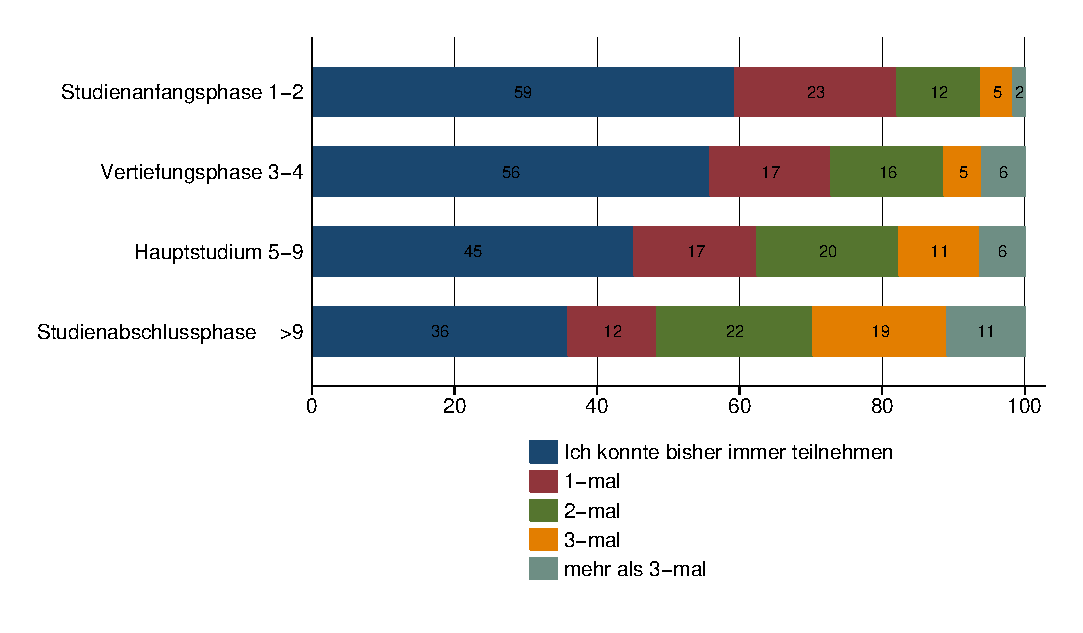
\includegraphics[
%  defaultresolution=72 !,
%  bmpsizefast=false
%]{image}
%\end{verbatim}
% \end{quote}
%
% \subsubsection{Hints}
%
% \begin{itemize}
% \item My version of \xfile{dvips.def} 1999/02/16 v3.0i defines
%       rules for the supported bitmap extensions, but does not
%       include them in the list of extensions that are tried
%       if the file name is not given with an extension.
%       In such a case, the list of extensions can be set
%       by \cs{DeclareGraphicsExtensions}, see \xpackage{grfguide}.
%       The following code just extends the list:
%       \begin{quote}
%\begin{verbatim}
%\makeatletter
%\g@addto@macro\Gin@extensions{,.bmp,.pcx,.msp}
%\makeatother
%\end{verbatim}
%       \end{quote}
% \item My version of \xfile{dvipdfm.def} 1998/11/24 vx.x misses
%       the graphics rule for PNG files. It can be added by:
%       \begin{quote}
%\begin{verbatim}
%\DeclareGraphicsRule{.png}{bmp}{.bb}{#1}
%\end{verbatim}
%       \end{quote}
%       See the previous issue to add the extension \xfile{.png} to the list
%       of extensions for package \xpackage{graphics}.
% \end{itemize}
%
% \subsubsection{Test program}
%
% There is a test program \xfile{bmpsize-test.tex}. Run it through
% \verb|latex|, \verb|pdflatex|, or \verb|pdftex|. Then given
% image files are inspected and the result is printed.
%
% \subsubsection{Interface for programmers}
%
% The macro names of the parsers are \verb|\bmpsize@read@|\meta{type}.
% Example: \cs{bmpsize@read@jpg} in case of JPEG.
%
% A parser sets the switch \cs{ifbmpsize@ok} to true, if it
% could successfully parse the image file.
% The width and height are returnd in \cs{bmpsize@width} and
% \cs{bmpsize@height}. If information about density is available,
% it is used to calculate width and height of the image, otherwise
% the values given by option \xoption{defaultresolution} is used.
% \xoption{resolution} overwrites the values in the image file.
%
% \subsection{Improved bitmap inclusion}
%
% Some drivers for package \xpackage{graphics} define the graphics
% type \xoption{bmp} for bitmap images. The code in the standard
% drivers for \xoption{dvips}, \xoption{dvipdfm}, and \xoption{dvipdfmx}
% is very basic and misses essential features of the
% package \xpackage{graphicx}. Therefore the code for bitmap
% inclusion is automatically rewritten by this package to add
% the following features:
% \begin{itemize}
% \item Support for \xoption{viewport} and \xoption{trim}.
% \item Support for \xoption{clip}.
% \item In case of \xoption{dvipdfm} and \xoption{dvipdfmx} the
%       bitmap images are reused and not included again if they
%       are used more than once.
% \end{itemize}
% However, there is a difference between \xoption{dvipdfm} and
% \xoption{dvipdfmx}, especially if images are reused. In the
% former case the reused box has width and height of 1bp, in the
% latter case its natural width. Thus the correct driver option must be given.
% \xoption{dvipdfm} and \xoption{dvipdfmx} are not equivalent.
%
% Older versions of \xoption{dvipdfmx} uses a size of 1in. However I do
% want to distinguish between versions of the same program. Therefore the
% support of these older versions has stopped with version 1.6 of this package.
% Use version dvipdfmx-20090708 or newer (some few versions before will
% probably also work, but I don't want to investigate this further).
%
% \StopEventually{
% }
%
% \section{Implementation}
%
% \subsection{Basic package \xpackage{bmpsize-base}}
%
%    Identification.
%    \begin{macrocode}
%<*base>
\ProvidesPackage{bmpsize-base}%
  [2009/09/04 v1.6 Basic part of bmpsize (HO)]%
%    \end{macrocode}
%    Modules of package \xpackage{fp} are used for calculations.
%    \begin{macrocode}
\RequirePackage{fp-basic}
\RequirePackage{fp-snap}
%    \end{macrocode}
%    Package \xpackage{fp} uses nested \cs{loop} structures.
%    That breaks with the plain-\TeX\ version of \cs{loop}.
%    Therefore we use the \LaTeX\ variant.
%    \begin{macro}{\@bmpsize@plain@loop}
%    \begin{macrocode}
\long\def\@bmpsize@plain@loop#1\repeat{%
  \def\iterate{%
    #1\relax
    \expandafter\iterate\fi
  }%
  \iterate
  \let\iterate\relax
}
%    \end{macrocode}
%    \end{macro}
%    \begin{macrocode}
\RequirePackage{pdftexcmds}[2007/11/11]
%    \end{macrocode}
%    \begin{macrocode}
\newif\ifbmpsize@ok
\let\@bmpsize@ok\bmpsize@oktrue

\newif\if@bmpsize@bigendian
\newif\if@bmpsize@absnum
\newif\if@bmpsize@user@resolution
\newif\if@bmpsize@fast
\@bmpsize@fasttrue

\def\@bmpsize@init{%
  \let\@bmpsize@org@plain@loop\loop
  \let\loop\@bmpsize@plain@loop
  \bmpsize@okfalse
  \@bmpsize@bigendiantrue
  \@bmpsize@absnumfalse
  \let\bmpsize@pixelwidth\relax
  \let\bmpsize@pixelheight\relax
  \let\bmpsize@pixelx\relax
  \let\bmpsize@pixely\relax
  \let\bmpsize@unit\relax
  \let\bmpsize@pixelxdenom\relax
  \let\bmpsize@pixelydenom\relax
  \let\bmpsize@orientation\relax
}

\def\@bmpsize@stop#1\@nil{}

\def\@bmpsize@loop#1{%
  #1%
  \@bmpsize@loop{#1}%
}
\def\@bmpsize@break#1\@bmpsize@loop#2{}

\def\@bmpsize@size#1#2#3{%
  \edef#3{\pdf@filesize{#1}}%
  \ifx#3\@empty
    \expandafter\@bmpsize@stop
  \fi
  \ifnum#3<#2\relax
    \expandafter\@bmpsize@stop
  \fi
}

\def\@bmpsize@read#1#2#3{%
  \edef\@bmpsize@buf{\pdf@filedump{#3}{#2}{#1}}%
  \edef\@bmpsize@temp{%
    \noexpand\@bmpsize@check@byte{#2}\@bmpsize@buf{}{}\noexpand\\%
  }%
  \@bmpsize@temp
}
\def\@bmpsize@fillbuf#1{%
  \ifx\@bmpsize@buf\@empty
    \expandafter\@firstofone
  \else
    \expandafter\@gobble
  \fi
  {%
    \edef\@bmpsize@buf{%
      \pdf@filedump{\bmpsize@offset}{\bmpsize@fillbuflength}{#1}%
    }%
    \ifx\@bmpsize@buf\@empty
      \expandafter\@bmpsize@stop
    \fi
    \edef\bmpsize@offset{\the\numexpr\bmpsize@offset+\bmpsize@fillbuflength}%
  }%
}
\def\bmpsize@fillbuflength{10}

\def\@bmpsize@append#1#2#3{%
  \edef#1{#2#3}%
}
\def\@bmpsize@pushback#1{%
  \edef\@bmpsize@buf{#1\@bmpsize@buf}%
}

\def\@bmpsize@iswhite#1{%
  \ifnum\pdf@strcmp{#1}{09}=\z@
  \else
    \ifnum\pdf@strcmp{#1}{0A}=\z@
    \else
      \ifnum\pdf@strcmp{#1}{0D}=\z@
      \else
        \ifnum\pdf@strcmp{#1}{20}=\z@
        \else
          1%
        \fi
      \fi
    \fi
  \fi
  \space
}
\def\@bmpsize@isdigit#1{%
  \ifnum\pdf@strcmp{#1}{30}<\z@
    1%
  \else
    \ifnum\pdf@strcmp{#1}{39}>\z@
      1%
    \fi
  \fi
  \space
}

\def\@bmpsize@check@byte#1#2#3{%
  \ifnum#1<\@ne
    \csname fi\endcsname
    \@bmpsize@cleanup@end
  \else
    \csname fi\endcsname
  \ifx!#2#3!%
    \csname fi\endcsname
    \@bmpsize@stop
  \else
    \csname fi\endcsname
    \expandafter\@bmpsize@check@byte\expandafter{\the\numexpr#1-1}%
}
\def\@bmpsize@cleanup@end#1\\{}

\def\@bmpsize@swap@maybe#1{%
  \if@bmpsize@bigendian
  \else
    \edef#1{\expandafter\@bmpsize@@swap#1\@empty\@empty\@empty\@empty}%
  \fi
}
\def\@bmpsize@@swap#1#2#3#4#5#6#7#8{%
  #7#8#5#6#3#4#1#2%
}

\def\@bmpsize@skip@one{%
  \edef\@bmpsize@buf{\expandafter\@gobbletwo\@bmpsize@buf}%
}
\def\@bmpsize@skip@two{%
  \edef\@bmpsize@buf{\expandafter\@gobblefour\@bmpsize@buf}%
}
\def\@bmpsize@skip@four{%
  \edef\@bmpsize@buf{%
    \expandafter\expandafter\expandafter\@gobblefour\expandafter
    \@gobblefour\@bmpsize@buf
  }%
}

\def\@bmpsize@grab#1#2{%
  \edef#1{\noexpand\@bmpsize@grab@byte#2=\@bmpsize@buf\noexpand\\}%
  \edef#1{#1}%
}
\def\@bmpsize@grab@byte#1=#2#3{%
  #2#3%
  \ifnum#1>\@ne
    \expandafter\@bmpsize@grab@byte\the\numexpr#1-1\expandafter=%
  \else
    \expandafter\@bmpsize@cleanup@end
  \fi
}

\def\@bmpsize@abs@maybe#1{%
  \let\@bmpsize@temp\relax
  \if@bmpsize@absnum
    \ifnum"\expandafter\@car#1\@nil>7 %
      \edef#1{\expandafter\@bmpsize@abs@byte#1\relax}%
      \ifnum\pdf@strcmp{#1}{7FFFFFFF}=\z@
        \let\@bmpsize@temp\@bmpsize@stop
      \else
        \def\@bmpsize@temp{\edef#1{\the\numexpr#1+1}}%
      \fi
    \fi
  \fi
}
\def\@bmpsize@abs@byte#1{%
  \ifx#1\relax
  \else
    \ifcase"0#1 %
      F\or E\or D\or C\or B\or A\or 9\or 8\or
      7\or 6\or 5\or 4\or 3\or 2\or 1\or 0%
    \fi
    \expandafter\@bmpsize@abs@byte
  \fi
}

\def\@bmpsize@num@one#1{%
  \@bmpsize@grab#11%
  \@bmpsize@abs@maybe#1%
  \edef#1{\number"#1}%
  \@bmpsize@temp
  \@bmpsize@skip@one
}
\def\@bmpsize@num@two#1{%
  \@bmpsize@grab#12%
  \@bmpsize@swap@maybe#1%
  \@bmpsize@abs@maybe#1%
  \edef#1{\number"#1}%
  \@bmpsize@temp
  \@bmpsize@skip@two
}
\def\@bmpsize@num@four#1{%
  \@bmpsize@grab#14%
  \@bmpsize@swap@maybe#1%
  \@bmpsize@abs@maybe#1%
  \ifnum\pdf@strcmp{#1}{7FFFFFFF}>\z@
    \expandafter\@bmpsize@stop
  \fi
  \edef#1{\number"#1}%
  \@bmpsize@temp
  \@bmpsize@skip@four
}

\def\@bmpsize@div#1#2#3{% #1 := #2/#3
  \FPdiv#1{#2}{#3}%
  \@bmpsize@beautify#1%
}
\def\@bmpsize@beautify#1{%
  \FPifint#1%
    \edef#1{\expandafter\@bmpsize@trunc#1.\@nil}%
  \else
    \edef#1{\expandafter\@bmpsize@cleanup@frac#1.\@nil}%
  \fi
}
\def\@bmpsize@trunc#1.#2\@nil{#1}
% #1 isn't an integer, thus we should have at least one
% necessary digit after the dot
\def\@bmpsize@cleanup@frac#1.#2#3.#4\@nil{%
  #1.#2%
  \ifx\\#3\\%
  \else
    \@bmpsize@cleanup@fracdigits#3000000000\@nil
  \fi
}
\def\@bmpsize@cleanup@fracdigits#1#2#3#4#5#6#7#8#9{%
  \ifcase#9 %
    \ifcase#8 %
      \ifcase#7 %
        \ifcase#6 %
          \ifcase#5 %
            \ifcase #4 %
              \ifcase #3 %
                \ifcase #2 %
                  \ifcase #1 %
                  \else
                    #1%
                  \fi
                \else
                  #1#2%
                \fi
              \else
                #1#2#3%
              \fi
            \else
              #1#2#3#4%
            \fi
          \else
            #1#2#3#4#5%
          \fi
        \else
          #1#2#3#4#5#6%
        \fi
      \else
        #1#2#3#4#5#6#7%
      \fi
    \else
      #1#2#3#4#5#6#7#8%
    \fi
  \else
    #1#2#3#4#5#6#7#8#9%
  \fi
  \@bmpsize@trunc.%
}

\def\@bmpsize@end{%
  \ifbmpsize@ok
    \ifx\bmpsize@pixelwidth\relax
      \bmpsize@okfalse
    \fi
    \ifx\bmpsize@pixelheight\relax
      \bmpsize@okfalse
    \fi
  \fi
  \ifbmpsize@ok
    \ifnum\bmpsize@pixelwidth>\z@
    \else
      \bmpsize@okfalse
    \fi
    \ifnum\bmpsize@pixelheight>\z@
    \else
      \bmpsize@okfalse
    \fi
  \fi
  \ifbmpsize@ok
    \ifcase 0%
      \ifx\bmpsize@pixelx\relax 1 \fi
      \ifx\bmpsize@pixely\relax 1 \fi
      \ifnum\bmpsize@pixelx>\z@\else 1 \fi
      \ifnum\bmpsize@pixely>\z@\else 1 \fi
      \ifx\bmpsize@pixelxdenom\relax
         \ifx\bmpsize@pixelydenom\relax\else 1 \fi
      \else
        \ifnum\bmpsize@pixelxdenom>\z@\else 1 \fi
      \fi
      \ifx\bmpsize@pixelydenom\relax
      \else
        \ifnum\bmpsize@pixelydenom>\z@\else 1 \fi
      \fi
    \else
      \let\bmpsize@pixelx\relax
      \let\bmpsize@pixely\relax
      \let\bmpsize@unit\relax
      \let\bmpsize@pixelxdenom\relax
      \let\bmpsize@pixelydenom\relax
    \fi
    \ifx\bmpsize@pixelxdenom\relax
    \else
      \@bmpsize@div\bmpsize@pixelx\bmpsize@pixelx\bmpsize@pixelxdenom
      \@bmpsize@div\bmpsize@pixely\bmpsize@pixely\bmpsize@pixelydenom
      \let\bmpsize@pixelxdenom\relax
      \let\bmpsize@pixelydenom\relax
    \fi
    \ifcase 0\ifx\bmpsize@unit\relax 1\fi
             \if@bmpsize@user@resolution 1\fi
             \relax
      \let\bmpsize@calc@unit\bmpsize@unit
      \let\bmpsize@calc@pixelx\bmpsize@pixelx
      \let\bmpsize@calc@pixely\bmpsize@pixely
    \else
      \let\bmpsize@calc@unit\bmpsize@unit@default
      \let\bmpsize@calc@pixelx\bmpsize@pixelx@default
      \let\bmpsize@calc@pixely\bmpsize@pixely@default
      \ifx\bmpsize@calc@pixely\Gin@exclamation
        \ifx\bmpsize@pixelx\relax
          \let\bmpsize@calc@pixely\bmpsize@calc@pixelx
        \else
          \FPdiv\bmpsize@calc@pixely\bmpsize@calc@pixelx\bmpsize@pixelx
          \FPmul\bmpsize@calc@pixely\bmpsize@calc@pixely\bmpsize@pixely
        \fi
      \else
        \ifx\bmpsize@calc@pixelx\Gin@exclamation
          \ifx\bmpsize@pixelx\relax
            \let\bmpsize@calc@pixelx\bmpsize@calc@pixely
          \else
            \FPdiv\bmpsize@calc@pixelx\bmpsize@calc@pixely\bmpsize@pixely
            \FPmul\bmpsize@calc@pixelx\bmpsize@calc@pixelx\bmpsize@pixelx
          \fi
        \fi
      \fi
    \fi
    \FPdiv\bmpsize@width\bmpsize@pixelwidth\bmpsize@calc@pixelx
    \FPdiv\bmpsize@height\bmpsize@pixelheight\bmpsize@calc@pixely
    % calculation of width and height in bp for package graphics
    % 1in = 72bp = 72.27pt, 72/72.27 = 8/8.03, 1pt = 65536sp
    \if@bmpsize@fast
      \edef\bmpsize@width{%
        \strip@pt\dimexpr.99626\dimexpr
        \bmpsize@width\dimexpr\bmpsize@calc@unit
      }%
      \edef\bmpsize@height{%
        \strip@pt\dimexpr.99626\dimexpr
        \bmpsize@height\dimexpr\bmpsize@calc@unit
      }%
    \else
      \edef\@bmpsize@temp{\number\dimexpr\bmpsize@calc@unit}%
      \ifnum\@bmpsize@temp>100000 %
        \FPmul\@bmpsize@temp\@bmpsize@temp{0.00001}%
        \def\@bmpsize@corr{100000}%
      \else
        \let\@bmpsize@corr\relax
      \fi
      \FPmul\bmpsize@width\bmpsize@width\@bmpsize@temp
      \FPmul\bmpsize@height\bmpsize@height\@bmpsize@temp
      \FPmul\bmpsize@width\bmpsize@width{8}%
      \FPmul\bmpsize@height\bmpsize@height{8}%
      \FPdiv\bmpsize@width\bmpsize@width{8.03}%
      \FPdiv\bmpsize@height\bmpsize@height{8.03}%
      \FPdiv\bmpsize@width\bmpsize@width{65536}%
      \FPdiv\bmpsize@height\bmpsize@height{65536}%
      \ifx\@bmpsize@corr\relax
      \else
        \FPmul\bmpsize@width\bmpsize@width\@bmpsize@corr
        \FPmul\bmpsize@height\bmpsize@height\@bmpsize@corr
      \fi
      \FPround\bmpsize@width\bmpsize@width{5}%
      \FPround\bmpsize@height\bmpsize@height{5}%
      \@bmpsize@beautify\bmpsize@width
      \@bmpsize@beautify\bmpsize@height
    \fi
  \fi
  \let\loop\@bmpsize@org@plain@loop
}
\def\bmpsize@unit@default{72.27pt}% more accurate than 1in
\def\bmpsize@pixelx@default{72}
\let\bmpsize@pixely@default\Gin@exclamation

\def\bmpsize@types{png,jpg,bmp,gif,tiff,pnm,pam,xpm,tga,pcx,msp,sgi}
%</base>
%    \end{macrocode}
%
% \subsection{Bitmap formats}
%
% \subsubsection{png}
%
%\iffalse
%<*ignore>
%\fi
%\begin{verbatim}
%begin png
%big-endian
%
%read 24 0
%grab 8        -> $temp
%check streq $temp [0x89 "PNG" 0x0D 0x0A 0x1A 0x0A]
%num 4         -> $length
%grab 4        -> $temp
%check streq $temp ["IHDR"]
%num 4         -> $pixelwidth
%num 4         -> $pixelheight
%ok
%assign numexpr(20 + $length) -> $offset
%loop
%  read 8 $offset
%  num 4       -> $length
%  grab 4      -> $temp
%  if streq $temp ["IDAT"]
%    stop
%  fi
%  if streq $temp ["pHYs"]
%    read 9 numexpr($offset + 8)
%    num 4     -> $pixelx
%    num 4     -> $pixely
%    grab 1     -> $temp
%    if numeq $temp 1
%      assign {100cm} -> $unit
%    fi
%    stop
%  fi
%  assign numexpr($offset + 12 + $length) -> $offset
%repeat
%end
%\end{verbatim}
%\iffalse
%</ignore>
%\fi
%    \begin{macro}{\bmpsize@read@png}
%    \begin{macrocode}
%<*base>
\def\bmpsize@read@png#1{%
  \@bmpsize@init
  \@bmpsize@bigendiantrue
  \@bmpsize@read{#1}{24}{0}%
  \@bmpsize@grab\bmpsize@temp{8}%
  \@bmpsize@skip@four
  \@bmpsize@skip@four
  \ifnum\pdf@strcmp{\bmpsize@temp}{89504E470D0A1A0A}=\z@
  \else
    \expandafter\@bmpsize@stop
  \fi
  \@bmpsize@num@four\bmpsize@length
  \@bmpsize@grab\bmpsize@temp{4}%
  \@bmpsize@skip@four
  \ifnum\pdf@strcmp{\bmpsize@temp}{49484452}=\z@
  \else
    \expandafter\@bmpsize@stop
  \fi
  \@bmpsize@num@four\bmpsize@pixelwidth
  \@bmpsize@num@four\bmpsize@pixelheight
  \@bmpsize@ok
  \edef\bmpsize@offset{\the\numexpr20+\bmpsize@length}%
  \@bmpsize@loop{%
    \@bmpsize@read{#1}{8}{\bmpsize@offset}%
    \@bmpsize@num@four\bmpsize@length
    \@bmpsize@grab\bmpsize@temp{4}%
    \@bmpsize@skip@four
    \ifnum\pdf@strcmp{\bmpsize@temp}{49444154}=\z@
      \expandafter\@firstofone
    \else
      \expandafter\@gobble
    \fi
    {%
      \@bmpsize@stop
    }%
    \ifnum\pdf@strcmp{\bmpsize@temp}{70485973}=\z@
      \expandafter\@firstofone
    \else
      \expandafter\@gobble
    \fi
    {%
      \@bmpsize@read{#1}{9}{\numexpr\bmpsize@offset+8\relax}%
      \@bmpsize@num@four\bmpsize@pixelx
      \@bmpsize@num@four\bmpsize@pixely
      \@bmpsize@grab\bmpsize@temp{1}%
      \@bmpsize@skip@one
      \ifnum\bmpsize@temp=1\relax
        \expandafter\@firstofone
      \else
        \expandafter\@gobble
      \fi
      {%
        \def\bmpsize@unit{100cm}%
      }%
      \@bmpsize@stop
    }%
    \edef\bmpsize@offset{\the\numexpr\bmpsize@offset+12+\bmpsize@length}%
  }%
  \@bmpsize@stop
  \@nil
  \@bmpsize@end
}%
%</base>
%    \end{macrocode}
%    \end{macro}
%
% \subsubsection{jpg}
%
%\iffalse
%<*ignore>
%\fi
%\begin{verbatim}
%begin jpg
%
%read 3 0
%grab 3      -> $temp % SOI and 0xFF
%check streq $temp [0xFF 0xD8 0xFF]
%assign {2} -> $offset
%assign {0} -> $exifdensity
%loop
%  read 4 $offset
%  grab 1    -> $temp
%  check streq $temp [0xFF]
%  num 1    -> $temp
%  if numeq $temp 0xDA % SOS
%    stop
%  fi
%  % look for JFIF APP0 segment
%  if numeq $temp 0xE0 % APP0
%    num 2       -> $length
%    if numeq $exifdensity 0
%      if numge $length 16 % a JFIF segment has 16 bytes at least
%        read 12 numexpr($offset + 4)
%        grab 5      -> $temp % identifier
%        if streq $temp ["JFIF" 0x0]
%          check numge $length 16
%          skip 2 % version
%          num 1       -> $temp % units
%          if numeq $temp 1
%            assign {72.27pt} -> $unit
%          else
%            if numeq $temp 2
%              assign {1cm} -> $unit
%            fi
%          fi
%          num 2    -> $pixelx
%          num 2    -> $pixely
%        fi
%      fi
%    fi
%  else
%    if numeq $temp 0xE1 % APP1
%      % look for Exif APP1 segment
%      num 2 -> $length
%      if numge $length 20 % identifier (6) + Tiff header (8) + first IFD (>=6)
%        read 20 numexpr($offset + 4)
%        grab 6 -> $temp
%        if streq $temp ["Exif" 0x0 0x0]
%          assign numexpr($offset + 10) -> $exifoffset
%          % read TIFF header
%          grab 2 -> $temp
%          if streq $temp ["II"]
%            little-endian
%          else
%            check streq $temp ["MM"]
%            % big-endian
%          fi
%          num 2 -> $temp
%          check numeq $temp 42
%          num 4 -> $temp % offset of first IFD
%          check numgt $temp 0
%          % read first IFD
%          assign numexpr($temp + $exifoffset) -> $off
%          read 2 $off
%          num 2 -> $entries
%          assign numexpr($off + 2) -> $off
%          loop
%            if numeq $entries 0
%              break
%            fi
%            assign numexpr($entries - 1) -> $entries
%            % entry format:
%            % 2 tag
%            % 2 field type
%            % 4 count
%            % 4 value/offset
%            read 12 $off
%            assign numexpr($off + 12) -> $off
%            num 2 -> $tag
%            if numeq $tag 296 % ResolutionUnit
%              skip 6 % type: 3 (short), count: 1
%              num 2 -> $temp
%              ifcase $temp
%              or % 1
%                clear $unit
%              or % 2
%                assign {72.27pt} -> $unit
%              or % 3
%                assign {1cm} -> $unit
%              else
%                clear $unit % unknown
%              fi
%              ifcase $temp
%              or % 1
%              or % 2
%                assign {1} -> $exifdensity
%              or % 3
%                assign {1} -> $exifdensity
%              else
%                assign $exifdensity -> $exifdensity
%              fi
%            fi
%            % 256 ImageWidth (use width of JPG part)
%            % 257 ImageHeight (use height of JPG part)
%            if numeq $tag 274 % Orientation
%              skip 6 % type: 3 (short), count: 1
%              num 2 -> $temp
%              if numge $temp 0 
%                if numle $temp 8
%                  assign $temp -> $orientation
%                fi
%              fi
%            fi
%            if numeq $tag 282 % XResolution
%              skip 6
%              num 4 -> $temp
%              read 8 numexpr($temp + $exifoffset)
%              num 4 -> $pixelx
%              num 4 -> $temp
%              if numeq $temp 1
%              else
%                assign numexpr($temp) -> $pixelxdenom
%                % div $pixelx $temp -> $pixelx
%              fi
%            fi
%            if numeq $tag 283 % YResolution
%              skip 6
%              num 4 -> $temp
%              read 8 numexpr($temp + $exifoffset)
%              num 4 -> $pixely
%              num 4 -> $temp
%              if numeq $temp 1
%              else
%                assign numexpr($temp) -> $pixelydenom
%                % div $pixely $temp -> $pixely
%              fi
%            fi
%          repeat
%          big-endian
%        fi
%      fi
%    else
%      assign numexpr($temp - 0xC0) -> $temp
%      ifcase $temp % SOF_0
%      or % SOF_1
%      or % SOF_2
%      or % SOF_3
%      or % DHT
%        assign {-1} -> $temp
%      or % SOF_5
%      or % SOF_6
%      or % SOF_7
%      or % JPG
%        assign {-1} -> $temp
%      or % SOF_9
%      or % SOF_10
%      or % SOF_11
%      or % DAC
%        assign {-1} -> $temp
%      or % SOF_13
%      or % SOF_14
%      or % SOF_15
%      else
%        assign {-1} -> $temp
%      fi
%      if numeq $temp -1
%      else
%        read 4 numexpr($offset + 5)
%        num 2  -> $pixelheight
%        num 2  -> $pixelwidth
%        if numeq $pixelheight 0
%          clear $pixelheight
%          stop
%        fi
%        ok
%        stop
%      fi
%      num 2 -> $length
%    fi
%  fi
%  assign numexpr($offset + $length + 2) -> $offset
%repeat
%end
%\end{verbatim}
%\iffalse
%</ignore>
%\fi
%    \begin{macro}{\bmpsize@read@jpg}
%    \begin{macrocode}
%<*base>
\def\bmpsize@read@jpg#1{%
  \@bmpsize@init
  \@bmpsize@read{#1}{3}{0}%
  \@bmpsize@grab\bmpsize@temp{3}%
  \@bmpsize@skip@two
  \@bmpsize@skip@one
  \ifnum\pdf@strcmp{\bmpsize@temp}{FFD8FF}=\z@
  \else
    \expandafter\@bmpsize@stop
  \fi
  \def\bmpsize@offset{2}%
  \def\bmpsize@exifdensity{0}%
  \@bmpsize@loop{%
    \@bmpsize@read{#1}{4}{\bmpsize@offset}%
    \@bmpsize@grab\bmpsize@temp{1}%
    \@bmpsize@skip@one
    \ifnum\pdf@strcmp{\bmpsize@temp}{FF}=\z@
    \else
      \expandafter\@bmpsize@stop
    \fi
    \@bmpsize@num@one\bmpsize@temp
    \ifnum\bmpsize@temp=218\relax
      \expandafter\@firstofone
    \else
      \expandafter\@gobble
    \fi
    {%
      \@bmpsize@stop
    }%
    \ifnum\bmpsize@temp=224\relax
      \expandafter\@firstoftwo
    \else
      \expandafter\@secondoftwo
    \fi
    {%
      \@bmpsize@num@two\bmpsize@length
      \ifnum\bmpsize@exifdensity=0\relax
        \expandafter\@firstofone
      \else
        \expandafter\@gobble
      \fi
      {%
        \unless\ifnum\bmpsize@length<16\relax
          \expandafter\@firstofone
        \else
          \expandafter\@gobble
        \fi
        {%
          \@bmpsize@read{#1}{12}{\numexpr\bmpsize@offset+4\relax}%
          \@bmpsize@grab\bmpsize@temp{5}%
          \@bmpsize@skip@four
          \@bmpsize@skip@one
          \ifnum\pdf@strcmp{\bmpsize@temp}{4A46494600}=\z@
            \expandafter\@firstofone
          \else
            \expandafter\@gobble
          \fi
          {%
            \ifnum\bmpsize@length<16\relax
              \expandafter\@bmpsize@stop
            \fi
            \@bmpsize@skip@two
            \@bmpsize@num@one\bmpsize@temp
            \ifnum\bmpsize@temp=1\relax
              \expandafter\@firstoftwo
            \else
              \expandafter\@secondoftwo
            \fi
            {%
              \def\bmpsize@unit{72.27pt}%
            }{%
              \ifnum\bmpsize@temp=2\relax
                \expandafter\@firstofone
              \else
                \expandafter\@gobble
              \fi
              {%
                \def\bmpsize@unit{1cm}%
              }%
            }%
            \@bmpsize@num@two\bmpsize@pixelx
            \@bmpsize@num@two\bmpsize@pixely
          }%
        }%
      }%
    }{%
      \ifnum\bmpsize@temp=225\relax
        \expandafter\@firstoftwo
      \else
        \expandafter\@secondoftwo
      \fi
      {%
        \@bmpsize@num@two\bmpsize@length
        \unless\ifnum\bmpsize@length<20\relax
          \expandafter\@firstofone
        \else
          \expandafter\@gobble
        \fi
        {%
          \@bmpsize@read{#1}{20}{\numexpr\bmpsize@offset+4\relax}%
          \@bmpsize@grab\bmpsize@temp{6}%
          \@bmpsize@skip@four
          \@bmpsize@skip@two
          \ifnum\pdf@strcmp{\bmpsize@temp}{457869660000}=\z@
            \expandafter\@firstofone
          \else
            \expandafter\@gobble
          \fi
          {%
            \edef\bmpsize@exifoffset{\the\numexpr\bmpsize@offset+10}%
            \@bmpsize@grab\bmpsize@temp{2}%
            \@bmpsize@skip@two
            \ifnum\pdf@strcmp{\bmpsize@temp}{4949}=\z@
              \expandafter\@firstoftwo
            \else
              \expandafter\@secondoftwo
            \fi
            {%
              \@bmpsize@bigendianfalse
            }{%
              \ifnum\pdf@strcmp{\bmpsize@temp}{4D4D}=\z@
              \else
                \expandafter\@bmpsize@stop
              \fi
            }%
            \@bmpsize@num@two\bmpsize@temp
            \ifnum\bmpsize@temp=42\relax
            \else
              \expandafter\@bmpsize@stop
            \fi
            \@bmpsize@num@four\bmpsize@temp
            \ifnum\bmpsize@temp>0\relax
            \else
              \expandafter\@bmpsize@stop
            \fi
            \edef\bmpsize@off{\the\numexpr\bmpsize@temp+\bmpsize@exifoffset}%
            \@bmpsize@read{#1}{2}{\bmpsize@off}%
            \@bmpsize@num@two\bmpsize@entries
            \edef\bmpsize@off{\the\numexpr\bmpsize@off+2}%
            \@bmpsize@loop{%
              \ifnum\bmpsize@entries=0\relax
                \expandafter\@firstofone
              \else
                \expandafter\@gobble
              \fi
              {%
                \@bmpsize@break
              }%
              \edef\bmpsize@entries{\the\numexpr\bmpsize@entries-1}%
              \@bmpsize@read{#1}{12}{\bmpsize@off}%
              \edef\bmpsize@off{\the\numexpr\bmpsize@off+12}%
              \@bmpsize@num@two\bmpsize@tag
              \ifnum\bmpsize@tag=296\relax
                \expandafter\@firstofone
              \else
                \expandafter\@gobble
              \fi
              {%
                \@bmpsize@skip@four
                \@bmpsize@skip@two
                \@bmpsize@num@two\bmpsize@temp
                \ifcase\bmpsize@temp\relax
                \or
                  \let\bmpsize@unit\relax
                \or
                  \def\bmpsize@unit{72.27pt}%
                \or
                  \def\bmpsize@unit{1cm}%
                \else
                  \let\bmpsize@unit\relax
                \fi
                \ifcase\bmpsize@temp\relax
                \or
                \or
                  \def\bmpsize@exifdensity{1}%
                \or
                  \def\bmpsize@exifdensity{1}%
                \else
                  \let\bmpsize@exifdensity\bmpsize@exifdensity
                \fi
              }%
              \ifnum\bmpsize@tag=274\relax
                \expandafter\@firstofone
              \else
                \expandafter\@gobble
              \fi
              {%
                \@bmpsize@skip@four
                \@bmpsize@skip@two
                \@bmpsize@num@two\bmpsize@temp
                \unless\ifnum\bmpsize@temp<0\relax
                  \expandafter\@firstofone
                \else
                  \expandafter\@gobble
                \fi
                {%
                  \unless\ifnum\bmpsize@temp>8\relax
                    \expandafter\@firstofone
                  \else
                    \expandafter\@gobble
                  \fi
                  {%
                    \let\bmpsize@orientation\bmpsize@temp
                  }%
                }%
              }%
              \ifnum\bmpsize@tag=282\relax
                \expandafter\@firstofone
              \else
                \expandafter\@gobble
              \fi
              {%
                \@bmpsize@skip@four
                \@bmpsize@skip@two
                \@bmpsize@num@four\bmpsize@temp
                \@bmpsize@read{#1}{8}{\numexpr\bmpsize@temp+\bmpsize@exifoffset\relax}%
                \@bmpsize@num@four\bmpsize@pixelx
                \@bmpsize@num@four\bmpsize@temp
                \ifnum\bmpsize@temp=1\relax
                  \expandafter\@gobble
                \else
                  \expandafter\@firstofone
                \fi
                {%
                  \edef\bmpsize@pixelxdenom{\the\numexpr\bmpsize@temp}%
                }%
              }%
              \ifnum\bmpsize@tag=283\relax
                \expandafter\@firstofone
              \else
                \expandafter\@gobble
              \fi
              {%
                \@bmpsize@skip@four
                \@bmpsize@skip@two
                \@bmpsize@num@four\bmpsize@temp
                \@bmpsize@read{#1}{8}{\numexpr\bmpsize@temp+\bmpsize@exifoffset\relax}%
                \@bmpsize@num@four\bmpsize@pixely
                \@bmpsize@num@four\bmpsize@temp
                \ifnum\bmpsize@temp=1\relax
                  \expandafter\@gobble
                \else
                  \expandafter\@firstofone
                \fi
                {%
                  \edef\bmpsize@pixelydenom{\the\numexpr\bmpsize@temp}%
                }%
              }%
            }%
            \@bmpsize@bigendiantrue
          }%
        }%
      }{%
        \edef\bmpsize@temp{\the\numexpr\bmpsize@temp-192}%
        \ifcase\bmpsize@temp\relax
        \or
        \or
        \or
        \or
          \def\bmpsize@temp{-1}%
        \or
        \or
        \or
        \or
          \def\bmpsize@temp{-1}%
        \or
        \or
        \or
        \or
          \def\bmpsize@temp{-1}%
        \or
        \or
        \or
        \else
          \def\bmpsize@temp{-1}%
        \fi
        \ifnum\bmpsize@temp=-1\relax
          \expandafter\@gobble
        \else
          \expandafter\@firstofone
        \fi
        {%
          \@bmpsize@read{#1}{4}{\numexpr\bmpsize@offset+5\relax}%
          \@bmpsize@num@two\bmpsize@pixelheight
          \@bmpsize@num@two\bmpsize@pixelwidth
          \ifnum\bmpsize@pixelheight=0\relax
            \expandafter\@firstofone
          \else
            \expandafter\@gobble
          \fi
          {%
            \let\bmpsize@pixelheight\relax
            \@bmpsize@stop
          }%
          \@bmpsize@ok
          \@bmpsize@stop
        }%
        \@bmpsize@num@two\bmpsize@length
      }%
    }%
    \edef\bmpsize@offset{\the\numexpr\bmpsize@offset+\bmpsize@length+2}%
  }%
  \@bmpsize@stop
  \@nil
  \@bmpsize@end
}%
%</base>
%    \end{macrocode}
%    \end{macro}
%
% \subsubsection{bmp}
%
%\iffalse
%<*ignore>
%\fi
%\begin{verbatim}
%begin bmp
%little-endian
%
%read 26 0
%grab 2 -> $temp
%check streq $temp ["BM"]
%skip 12
%% header size is 4 bytes in V3+, unknown for V1, V2,
%% known header sizes fit in 2 bytes
%num 2   -> $temp
%if numeq $temp 12 % V1
%  skip 2
%  num 2 -> $pixelwidth
%  num 2 -> $pixelheight
%  % no resolution entries
%  ok
%  stop
%fi
%if numeq $temp 64 % V2
%  skip 2
%  num 2 -> $pixelwidth
%  num 2 -> $pixelheight
%  % missing specification for resolution
%  ok
%  stop
%fi
%% V3, V4, V5
%skip 2
%num 4 -> $pixelwidth
%absnum 4 -> $pixelheight
%ok
%read 8 38
%num 4 -> $pixelx
%num 4 -> $pixely
%assign {100cm} -> $unit
%end
%\end{verbatim}
%\iffalse
%</ignore>
%\fi
%    \begin{macro}{\bmpsize@read@bmp}
%    \begin{macrocode}
%<*base>
\def\bmpsize@read@bmp#1{%
  \@bmpsize@init
  \@bmpsize@bigendianfalse
  \@bmpsize@read{#1}{26}{0}%
  \@bmpsize@grab\bmpsize@temp{2}%
  \@bmpsize@skip@two
  \ifnum\pdf@strcmp{\bmpsize@temp}{424D}=\z@
  \else
    \expandafter\@bmpsize@stop
  \fi
  \@bmpsize@skip@four
  \@bmpsize@skip@four
  \@bmpsize@skip@four
  \@bmpsize@num@two\bmpsize@temp
  \ifnum\bmpsize@temp=12\relax
    \expandafter\@firstofone
  \else
    \expandafter\@gobble
  \fi
  {%
    \@bmpsize@skip@two
    \@bmpsize@num@two\bmpsize@pixelwidth
    \@bmpsize@num@two\bmpsize@pixelheight
    \@bmpsize@ok
    \@bmpsize@stop
  }%
  \ifnum\bmpsize@temp=64\relax
    \expandafter\@firstofone
  \else
    \expandafter\@gobble
  \fi
  {%
    \@bmpsize@skip@two
    \@bmpsize@num@two\bmpsize@pixelwidth
    \@bmpsize@num@two\bmpsize@pixelheight
    \@bmpsize@ok
    \@bmpsize@stop
  }%
  \@bmpsize@skip@two
  \@bmpsize@num@four\bmpsize@pixelwidth
  \@bmpsize@absnumtrue
  \@bmpsize@num@four\bmpsize@pixelheight
  \@bmpsize@absnumfalse
  \@bmpsize@ok
  \@bmpsize@read{#1}{8}{38}%
  \@bmpsize@num@four\bmpsize@pixelx
  \@bmpsize@num@four\bmpsize@pixely
  \def\bmpsize@unit{100cm}%
  \@bmpsize@stop
  \@nil
  \@bmpsize@end
}%
%</base>
%    \end{macrocode}
%    \end{macro}
%
% \subsubsection{gif}
%
%\iffalse
%<*ignore>
%\fi
%\begin{verbatim}
%begin gif
%little-endian
%
%% Header
%read 13 0
%grab 3      -> $temp
%check streq $temp ["GIF"]
%skip 3      % version
%
%% Logical Screen Descriptor
%num 2       -> $pixelwidth
%num 2       -> $pixelheight
%skip 2
%num 1       -> $temp % Pixel Aspect Ratio
%if numeq $temp 0
%else
%  assign numexpr($temp + 15) -> $pixelx
%  assign {64}     -> $pixely
%fi
%ok
%end
%\end{verbatim}
%\iffalse
%</ignore>
%\fi
%    \begin{macro}{\bmpsize@read@gif}
%    \begin{macrocode}
%<*base>
\def\bmpsize@read@gif#1{%
  \@bmpsize@init
  \@bmpsize@bigendianfalse
  \@bmpsize@read{#1}{13}{0}%
  \@bmpsize@grab\bmpsize@temp{3}%
  \@bmpsize@skip@two
  \@bmpsize@skip@one
  \ifnum\pdf@strcmp{\bmpsize@temp}{474946}=\z@
  \else
    \expandafter\@bmpsize@stop
  \fi
  \@bmpsize@skip@two
  \@bmpsize@skip@one
  \@bmpsize@num@two\bmpsize@pixelwidth
  \@bmpsize@num@two\bmpsize@pixelheight
  \@bmpsize@skip@two
  \@bmpsize@num@one\bmpsize@temp
  \ifnum\bmpsize@temp=0\relax
    \expandafter\@gobble
  \else
    \expandafter\@firstofone
  \fi
  {%
    \edef\bmpsize@pixelx{\the\numexpr\bmpsize@temp+15}%
    \def\bmpsize@pixely{64}%
  }%
  \@bmpsize@ok
  \@bmpsize@stop
  \@nil
  \@bmpsize@end
}%
%</base>
%    \end{macrocode}
%    \end{macro}
%
% \subsubsection{tiff}
%
%\iffalse
%<*ignore>
%\fi
%\begin{verbatim}
%begin tiff
%% defaults
%assign {72.27pt} -> $unit
%
%% Image File Header
%read 8 0
%grab 2 -> $temp
%if streq $temp ["II"]
%  little-endian
%else
%  check streq $temp ["MM"]
%  big-endian
%fi
%num 2 -> $temp
%check numeq $temp 42
%num 4 -> $offset % first IFD (Image File Directory)
%
%% First IFD
%read 2 $offset
%assign numexpr($offset + 2) -> $offset
%num 2 -> $entries
%ok % must rely on checks at the end
%loop
%  if numeq $entries 0
%    stop
%  fi
%  assign numexpr($entries - 1) -> $entries
%  % entry format:
%  % 2 tag
%  % 2 field type
%  % 4 count
%  % 4 value/offset
%  read 12 $offset
%  assign numexpr($offset + 12) -> $offset
%  num 2 -> $tag % tag
%  if numeq $temp 296 % ResolutionUnit
%    skip 6 % type: 3 (short), count: 1
%    num 2 -> $temp
%    ifcase $temp
%    or % 1
%      clear $unit
%    or % 2
%      assign {72.27pt} -> $unit
%    or % 3
%      assign {1cm} -> $unit
%    else
%      clear $unit
%    fi
%  fi
%  if numeq $tag 256 % ImageWidth
%    skip 6
%    num 4 -> $pixelwidth
%  fi
%  if numeq $tag 257 % ImageLength
%    skip 6
%    num 4 -> $pixelheight
%  fi
%  if numeq $tag 282 % XResolution
%    skip 6
%    num 4 -> $temp
%    read 8 $temp
%    num 4 -> $pixelx
%    num 4 -> $temp
%    if numeq $temp 1
%    else
%      assign numexpr($temp) -> $pixelxdenom
%      % div $pixelx $temp -> $pixelx
%    fi
%  fi
%  if numeq $tag 283 % YResolution
%    skip 6
%    num 4 -> $temp
%    read 8 $temp
%    num 4 -> $pixely
%    num 4 -> $temp
%    if numeq $temp 1
%    else
%      assign numexpr($temp) -> $pixelydenom
%      % div $pixely $temp -> $pixely
%    fi
%  fi
%repeat
%end
%\end{verbatim}
%\iffalse
%</ignore>
%\fi
%    \begin{macro}{\bmpsize@read@tiff}
%    \begin{macrocode}
%<*base>
\def\bmpsize@read@tiff#1{%
  \@bmpsize@init
  \def\bmpsize@unit{72.27pt}%
  \@bmpsize@read{#1}{8}{0}%
  \@bmpsize@grab\bmpsize@temp{2}%
  \@bmpsize@skip@two
  \ifnum\pdf@strcmp{\bmpsize@temp}{4949}=\z@
    \expandafter\@firstoftwo
  \else
    \expandafter\@secondoftwo
  \fi
  {%
    \@bmpsize@bigendianfalse
  }{%
    \ifnum\pdf@strcmp{\bmpsize@temp}{4D4D}=\z@
    \else
      \expandafter\@bmpsize@stop
    \fi
    \@bmpsize@bigendiantrue
  }%
  \@bmpsize@num@two\bmpsize@temp
  \ifnum\bmpsize@temp=42\relax
  \else
    \expandafter\@bmpsize@stop
  \fi
  \@bmpsize@num@four\bmpsize@offset
  \@bmpsize@read{#1}{2}{\bmpsize@offset}%
  \edef\bmpsize@offset{\the\numexpr\bmpsize@offset+2}%
  \@bmpsize@num@two\bmpsize@entries
  \@bmpsize@ok
  \@bmpsize@loop{%
    \ifnum\bmpsize@entries=0\relax
      \expandafter\@firstofone
    \else
      \expandafter\@gobble
    \fi
    {%
      \@bmpsize@stop
    }%
    \edef\bmpsize@entries{\the\numexpr\bmpsize@entries-1}%
    \@bmpsize@read{#1}{12}{\bmpsize@offset}%
    \edef\bmpsize@offset{\the\numexpr\bmpsize@offset+12}%
    \@bmpsize@num@two\bmpsize@tag
    \ifnum\bmpsize@temp=296\relax
      \expandafter\@firstofone
    \else
      \expandafter\@gobble
    \fi
    {%
      \@bmpsize@skip@four
      \@bmpsize@skip@two
      \@bmpsize@num@two\bmpsize@temp
      \ifcase\bmpsize@temp\relax
      \or
        \let\bmpsize@unit\relax
      \or
        \def\bmpsize@unit{72.27pt}%
      \or
        \def\bmpsize@unit{1cm}%
      \else
        \let\bmpsize@unit\relax
      \fi
    }%
    \ifnum\bmpsize@tag=256\relax
      \expandafter\@firstofone
    \else
      \expandafter\@gobble
    \fi
    {%
      \@bmpsize@skip@four
      \@bmpsize@skip@two
      \@bmpsize@num@four\bmpsize@pixelwidth
    }%
    \ifnum\bmpsize@tag=257\relax
      \expandafter\@firstofone
    \else
      \expandafter\@gobble
    \fi
    {%
      \@bmpsize@skip@four
      \@bmpsize@skip@two
      \@bmpsize@num@four\bmpsize@pixelheight
    }%
    \ifnum\bmpsize@tag=282\relax
      \expandafter\@firstofone
    \else
      \expandafter\@gobble
    \fi
    {%
      \@bmpsize@skip@four
      \@bmpsize@skip@two
      \@bmpsize@num@four\bmpsize@temp
      \@bmpsize@read{#1}{8}{\bmpsize@temp}%
      \@bmpsize@num@four\bmpsize@pixelx
      \@bmpsize@num@four\bmpsize@temp
      \ifnum\bmpsize@temp=1\relax
        \expandafter\@gobble
      \else
        \expandafter\@firstofone
      \fi
      {%
        \edef\bmpsize@pixelxdenom{\the\numexpr\bmpsize@temp}%
      }%
    }%
    \ifnum\bmpsize@tag=283\relax
      \expandafter\@firstofone
    \else
      \expandafter\@gobble
    \fi
    {%
      \@bmpsize@skip@four
      \@bmpsize@skip@two
      \@bmpsize@num@four\bmpsize@temp
      \@bmpsize@read{#1}{8}{\bmpsize@temp}%
      \@bmpsize@num@four\bmpsize@pixely
      \@bmpsize@num@four\bmpsize@temp
      \ifnum\bmpsize@temp=1\relax
        \expandafter\@gobble
      \else
        \expandafter\@firstofone
      \fi
      {%
        \edef\bmpsize@pixelydenom{\the\numexpr\bmpsize@temp}%
      }%
    }%
  }%
  \@bmpsize@stop
  \@nil
  \@bmpsize@end
}%
%</base>
%    \end{macrocode}
%    \end{macro}
%
% \subsubsection{pnm}
%
%\iffalse
%<*ignore>
%\fi
%\begin{verbatim}
%begin pnm
%assign {0} -> $offset
%read 3 $offset
%assign {3} -> $offset
%grab 1 -> $temp
%check streq $temp ["P"]
%grab 1 -> $temp
%check strge $temp ["1"]
%check strle $temp ["6"]
%% ensure one white space
%grab 1 -> $temp
%if iswhite $temp
%else
%  stop
%fi
%loop
%  % skip white space
%  fillbuf
%  grab 1 -> $temp
%  if iswhite $temp
%  else
%    if streq $temp ["#"]
%      % ignore comments
%      loop
%        fillbuf
%        grab 1 -> $temp
%        if streq $temp [0x0A]
%          break
%        else
%          if streq $temp [0x0D]
%            break
%          fi
%        fi
%      repeat
%    else
%      pushback $temp
%      break
%    fi
%  fi
%repeat
%assign {} -> $tempnum
%loop
%  fillbuf
%  grab 1 -> $temp
%  if isdigit $temp
%    append $tempnum $temp -> $tempnum
%  else
%    if iswhite $temp
%      break
%    else
%      stop
%    fi
%  fi
%repeat
%assign unescapehex($tempnum) -> $pixelwidth
%loop
%  fillbuf
%  grab 1 -> $temp
%  if iswhite $temp
%  else
%    pushback $temp
%    break
%  fi
%repeat
%assign {} -> $tempnum
%loop
%  fillbuf
%  grab 1 -> $temp
%  if isdigit $temp
%    append $tempnum $temp -> $tempnum
%  else
%    if iswhite $temp
%      break
%    else
%      stop
%    fi
%  fi
%repeat
%assign unescapehex($tempnum) -> $pixelheight
%ok
%end
%\end{verbatim}
%\iffalse
%</ignore>
%\fi
%    \begin{macro}{\bmpsize@read@pnm}
%    \begin{macrocode}
%<*base>
\def\bmpsize@read@pnm#1{%
  \@bmpsize@init
  \def\bmpsize@offset{0}%
  \@bmpsize@read{#1}{3}{\bmpsize@offset}%
  \def\bmpsize@offset{3}%
  \@bmpsize@grab\bmpsize@temp{1}%
  \@bmpsize@skip@one
  \ifnum\pdf@strcmp{\bmpsize@temp}{50}=\z@
  \else
    \expandafter\@bmpsize@stop
  \fi
  \@bmpsize@grab\bmpsize@temp{1}%
  \@bmpsize@skip@one
  \ifnum\pdf@strcmp{\bmpsize@temp}{31}<\z@
    \expandafter\@bmpsize@stop
  \fi
  \ifnum\pdf@strcmp{\bmpsize@temp}{36}>\z@
    \expandafter\@bmpsize@stop
  \fi
  \@bmpsize@grab\bmpsize@temp{1}%
  \@bmpsize@skip@one
  \ifcase 0\@bmpsize@iswhite\bmpsize@temp
    \expandafter\@gobble
  \else
    \expandafter\@firstofone
  \fi
  {%
    \@bmpsize@stop
  }%
  \@bmpsize@loop{%
    \@bmpsize@fillbuf{#1}%
    \@bmpsize@grab\bmpsize@temp{1}%
    \@bmpsize@skip@one
    \ifcase 0\@bmpsize@iswhite\bmpsize@temp
      \expandafter\@gobble
    \else
      \expandafter\@firstofone
    \fi
    {%
      \ifnum\pdf@strcmp{\bmpsize@temp}{23}=\z@
        \expandafter\@firstoftwo
      \else
        \expandafter\@secondoftwo
      \fi
      {%
        \@bmpsize@loop{%
          \@bmpsize@fillbuf{#1}%
          \@bmpsize@grab\bmpsize@temp{1}%
          \@bmpsize@skip@one
          \ifnum\pdf@strcmp{\bmpsize@temp}{0A}=\z@
            \expandafter\@firstoftwo
          \else
            \expandafter\@secondoftwo
          \fi
          {%
            \@bmpsize@break
          }{%
            \ifnum\pdf@strcmp{\bmpsize@temp}{0D}=\z@
              \expandafter\@firstofone
            \else
              \expandafter\@gobble
            \fi
            {%
              \@bmpsize@break
            }%
          }%
        }%
      }{%
        \@bmpsize@pushback\bmpsize@temp
        \@bmpsize@break
      }%
    }%
  }%
  \def\bmpsize@tempnum{}%
  \@bmpsize@loop{%
    \@bmpsize@fillbuf{#1}%
    \@bmpsize@grab\bmpsize@temp{1}%
    \@bmpsize@skip@one
    \ifcase 0\@bmpsize@isdigit\bmpsize@temp
      \expandafter\@firstoftwo
    \else
      \expandafter\@secondoftwo
    \fi
    {%
      \@bmpsize@append\bmpsize@tempnum\bmpsize@tempnum\bmpsize@temp
    }{%
      \ifcase 0\@bmpsize@iswhite\bmpsize@temp
        \expandafter\@firstoftwo
      \else
        \expandafter\@secondoftwo
      \fi
      {%
        \@bmpsize@break
      }{%
        \@bmpsize@stop
      }%
    }%
  }%
  \edef\bmpsize@pixelwidth{\pdf@unescapehex{\bmpsize@tempnum}}%
  \@bmpsize@loop{%
    \@bmpsize@fillbuf{#1}%
    \@bmpsize@grab\bmpsize@temp{1}%
    \@bmpsize@skip@one
    \ifcase 0\@bmpsize@iswhite\bmpsize@temp
      \expandafter\@gobble
    \else
      \expandafter\@firstofone
    \fi
    {%
      \@bmpsize@pushback\bmpsize@temp
      \@bmpsize@break
    }%
  }%
  \def\bmpsize@tempnum{}%
  \@bmpsize@loop{%
    \@bmpsize@fillbuf{#1}%
    \@bmpsize@grab\bmpsize@temp{1}%
    \@bmpsize@skip@one
    \ifcase 0\@bmpsize@isdigit\bmpsize@temp
      \expandafter\@firstoftwo
    \else
      \expandafter\@secondoftwo
    \fi
    {%
      \@bmpsize@append\bmpsize@tempnum\bmpsize@tempnum\bmpsize@temp
    }{%
      \ifcase 0\@bmpsize@iswhite\bmpsize@temp
        \expandafter\@firstoftwo
      \else
        \expandafter\@secondoftwo
      \fi
      {%
        \@bmpsize@break
      }{%
        \@bmpsize@stop
      }%
    }%
  }%
  \edef\bmpsize@pixelheight{\pdf@unescapehex{\bmpsize@tempnum}}%
  \@bmpsize@ok
  \@bmpsize@stop
  \@nil
  \@bmpsize@end
}%
%</base>
%    \end{macrocode}
%    \end{macro}
%
% \subsubsection{pam}
%
%\iffalse
%<*ignore>
%\fi
%\begin{verbatim}
%begin pam
%read 3 0
%assign {3} -> $offset
%assign $offset -> $off
%grab 3 -> $temp
%check streq $temp ["P7" 0x0A]
%loop
%  fillbuf
%  grab 1 -> $temp
%  if iswhite $temp
%    % ignore white space
%    assign numexpr($off + 1) -> $off
%  else
%    if streq $temp ["#"]
%      % ignore comment line
%      assign numexpr($off + 1) -> $off
%      loop
%        fillbuf
%        grab 1 -> $temp
%        assign numexpr($off + 1) -> $off
%        if streq $temp [0x0A]
%          break
%        fi
%      repeat
%    else
%      read 6 $off
%      assign numexpr($off + 6) -> $offset
%      grab 5 -> $head
%      if streq $head ["WIDTH"]
%        assign numexpr($off + 5) -> $off
%        % skip white space
%        loop
%          fillbuf
%          grab 1 -> $temp
%          if iswhite $temp
%            assign numexpr($off + 1) -> $off
%          else
%            if isdigit $temp
%              assign numexpr($off + 1) -> $off
%              break
%            else
%              % error
%              stop
%            fi
%          fi
%        repeat
%        % read number
%        assign $temp -> $tempnum
%        loop
%          fillbuf
%          grab 1 -> $temp
%          if isdigit $temp
%            assign numexpr($off + 1) -> $off
%            append $tempnum $temp -> $tempnum
%          else
%            pushback $temp
%            break
%          fi
%        repeat
%        % skip to end of line
%        loop
%          fillbuf
%          grab 1 -> $temp
%          assign numexpr($off + 1) -> $off
%          if streq $temp [0x0A]
%            break
%          fi
%        repeat
%        assign unescapehex($tempnum) -> $pixelwidth
%      else
%        grab 1 -> $temp
%        append $head $temp -> $head
%        if streq $head ["ENDHDR"]
%          % last header line
%          ok
%          stop
%        else
%          if streq $head ["HEIGHT"]
%            assign numexpr($off + 6) -> $off
%            % skip white space
%            loop
%              fillbuf
%              grab 1 -> $temp
%              if iswhite $temp
%                assign numexpr($off + 1) -> $off
%              else
%                if isdigit $temp
%                  assign numexpr($off + 1) -> $off
%                  break
%                else
%                  % error
%                  stop
%                fi
%              fi
%            repeat
%            % read number
%            assign $temp -> $tempnum
%            loop
%              fillbuf
%              grab 1 -> $temp
%              if isdigit $temp
%                assign numexpr($off + 1) -> $off
%                append $tempnum $temp -> $tempnum
%              else
%                pushback $temp
%                break
%              fi
%            repeat
%            % skip to end of line
%            loop
%              fillbuf
%              grab 1 -> $temp
%              assign numexpr($off + 1) -> $off
%              if streq $temp [0x0A]
%                break
%              fi
%            repeat
%            assign unescapehex($tempnum) -> $pixelheight
%          else
%            % ignore unknown header line
%            pushback $head
%            loop
%              fillbuf
%              grab 1 -> $temp
%              assign numexpr($off + 1) -> $off
%              if streq $temp [0x0A]
%                break
%              fi
%            repeat
%          fi
%        fi
%      fi
%    fi
%  fi
%repeat
%end
%\end{verbatim}
%\iffalse
%</ignore>
%\fi
%    \begin{macro}{\bmpsize@read@pam}
%    \begin{macrocode}
%<*base>
\def\bmpsize@read@pam#1{%
  \@bmpsize@init
  \@bmpsize@read{#1}{3}{0}%
  \def\bmpsize@offset{3}%
  \let\bmpsize@off\bmpsize@offset
  \@bmpsize@grab\bmpsize@temp{3}%
  \@bmpsize@skip@two
  \@bmpsize@skip@one
  \ifnum\pdf@strcmp{\bmpsize@temp}{50370A}=\z@
  \else
    \expandafter\@bmpsize@stop
  \fi
  \@bmpsize@loop{%
    \@bmpsize@fillbuf{#1}%
    \@bmpsize@grab\bmpsize@temp{1}%
    \@bmpsize@skip@one
    \ifcase 0\@bmpsize@iswhite\bmpsize@temp
      \expandafter\@firstoftwo
    \else
      \expandafter\@secondoftwo
    \fi
    {%
      \edef\bmpsize@off{\the\numexpr\bmpsize@off+1}%
    }{%
      \ifnum\pdf@strcmp{\bmpsize@temp}{23}=\z@
        \expandafter\@firstoftwo
      \else
        \expandafter\@secondoftwo
      \fi
      {%
        \edef\bmpsize@off{\the\numexpr\bmpsize@off+1}%
        \@bmpsize@loop{%
          \@bmpsize@fillbuf{#1}%
          \@bmpsize@grab\bmpsize@temp{1}%
          \@bmpsize@skip@one
          \edef\bmpsize@off{\the\numexpr\bmpsize@off+1}%
          \ifnum\pdf@strcmp{\bmpsize@temp}{0A}=\z@
            \expandafter\@firstofone
          \else
            \expandafter\@gobble
          \fi
          {%
            \@bmpsize@break
          }%
        }%
      }{%
        \@bmpsize@read{#1}{6}{\bmpsize@off}%
        \edef\bmpsize@offset{\the\numexpr\bmpsize@off+6}%
        \@bmpsize@grab\bmpsize@head{5}%
        \@bmpsize@skip@four
        \@bmpsize@skip@one
        \ifnum\pdf@strcmp{\bmpsize@head}{5749445448}=\z@
          \expandafter\@firstoftwo
        \else
          \expandafter\@secondoftwo
        \fi
        {%
          \edef\bmpsize@off{\the\numexpr\bmpsize@off+5}%
          \@bmpsize@loop{%
            \@bmpsize@fillbuf{#1}%
            \@bmpsize@grab\bmpsize@temp{1}%
            \@bmpsize@skip@one
            \ifcase 0\@bmpsize@iswhite\bmpsize@temp
              \expandafter\@firstoftwo
            \else
              \expandafter\@secondoftwo
            \fi
            {%
              \edef\bmpsize@off{\the\numexpr\bmpsize@off+1}%
            }{%
              \ifcase 0\@bmpsize@isdigit\bmpsize@temp
                \expandafter\@firstoftwo
              \else
                \expandafter\@secondoftwo
              \fi
              {%
                \edef\bmpsize@off{\the\numexpr\bmpsize@off+1}%
                \@bmpsize@break
              }{%
                \@bmpsize@stop
              }%
            }%
          }%
          \let\bmpsize@tempnum\bmpsize@temp
          \@bmpsize@loop{%
            \@bmpsize@fillbuf{#1}%
            \@bmpsize@grab\bmpsize@temp{1}%
            \@bmpsize@skip@one
            \ifcase 0\@bmpsize@isdigit\bmpsize@temp
              \expandafter\@firstoftwo
            \else
              \expandafter\@secondoftwo
            \fi
            {%
              \edef\bmpsize@off{\the\numexpr\bmpsize@off+1}%
              \@bmpsize@append\bmpsize@tempnum\bmpsize@tempnum\bmpsize@temp
            }{%
              \@bmpsize@pushback\bmpsize@temp
              \@bmpsize@break
            }%
          }%
          \@bmpsize@loop{%
            \@bmpsize@fillbuf{#1}%
            \@bmpsize@grab\bmpsize@temp{1}%
            \@bmpsize@skip@one
            \edef\bmpsize@off{\the\numexpr\bmpsize@off+1}%
            \ifnum\pdf@strcmp{\bmpsize@temp}{0A}=\z@
              \expandafter\@firstofone
            \else
              \expandafter\@gobble
            \fi
            {%
              \@bmpsize@break
            }%
          }%
          \edef\bmpsize@pixelwidth{\pdf@unescapehex{\bmpsize@tempnum}}%
        }{%
          \@bmpsize@grab\bmpsize@temp{1}%
          \@bmpsize@skip@one
          \@bmpsize@append\bmpsize@head\bmpsize@head\bmpsize@temp
          \ifnum\pdf@strcmp{\bmpsize@head}{454E44484452}=\z@
            \expandafter\@firstoftwo
          \else
            \expandafter\@secondoftwo
          \fi
          {%
            \@bmpsize@ok
            \@bmpsize@stop
          }{%
            \ifnum\pdf@strcmp{\bmpsize@head}{484549474854}=\z@
              \expandafter\@firstoftwo
            \else
              \expandafter\@secondoftwo
            \fi
            {%
              \edef\bmpsize@off{\the\numexpr\bmpsize@off+6}%
              \@bmpsize@loop{%
                \@bmpsize@fillbuf{#1}%
                \@bmpsize@grab\bmpsize@temp{1}%
                \@bmpsize@skip@one
                \ifcase 0\@bmpsize@iswhite\bmpsize@temp
                  \expandafter\@firstoftwo
                \else
                  \expandafter\@secondoftwo
                \fi
                {%
                  \edef\bmpsize@off{\the\numexpr\bmpsize@off+1}%
                }{%
                  \ifcase 0\@bmpsize@isdigit\bmpsize@temp
                    \expandafter\@firstoftwo
                  \else
                    \expandafter\@secondoftwo
                  \fi
                  {%
                    \edef\bmpsize@off{\the\numexpr\bmpsize@off+1}%
                    \@bmpsize@break
                  }{%
                    \@bmpsize@stop
                  }%
                }%
              }%
              \let\bmpsize@tempnum\bmpsize@temp
              \@bmpsize@loop{%
                \@bmpsize@fillbuf{#1}%
                \@bmpsize@grab\bmpsize@temp{1}%
                \@bmpsize@skip@one
                \ifcase 0\@bmpsize@isdigit\bmpsize@temp
                  \expandafter\@firstoftwo
                \else
                  \expandafter\@secondoftwo
                \fi
                {%
                  \edef\bmpsize@off{\the\numexpr\bmpsize@off+1}%
                  \@bmpsize@append\bmpsize@tempnum\bmpsize@tempnum\bmpsize@temp
                }{%
                  \@bmpsize@pushback\bmpsize@temp
                  \@bmpsize@break
                }%
              }%
              \@bmpsize@loop{%
                \@bmpsize@fillbuf{#1}%
                \@bmpsize@grab\bmpsize@temp{1}%
                \@bmpsize@skip@one
                \edef\bmpsize@off{\the\numexpr\bmpsize@off+1}%
                \ifnum\pdf@strcmp{\bmpsize@temp}{0A}=\z@
                  \expandafter\@firstofone
                \else
                  \expandafter\@gobble
                \fi
                {%
                  \@bmpsize@break
                }%
              }%
              \edef\bmpsize@pixelheight{\pdf@unescapehex{\bmpsize@tempnum}}%
            }{%
              \@bmpsize@pushback\bmpsize@head
              \@bmpsize@loop{%
                \@bmpsize@fillbuf{#1}%
                \@bmpsize@grab\bmpsize@temp{1}%
                \@bmpsize@skip@one
                \edef\bmpsize@off{\the\numexpr\bmpsize@off+1}%
                \ifnum\pdf@strcmp{\bmpsize@temp}{0A}=\z@
                  \expandafter\@firstofone
                \else
                  \expandafter\@gobble
                \fi
                {%
                  \@bmpsize@break
                }%
              }%
            }%
          }%
        }%
      }%
    }%
  }%
  \@bmpsize@stop
  \@nil
  \@bmpsize@end
}%
%</base>
%    \end{macrocode}
%    \end{macro}
%
% \subsubsection{xpm}
%
%\iffalse
%<*ignore>
%\fi
%\begin{verbatim}
%begin xpm
%read 9 0
%grab 9 -> $temp
%assign {9} -> $offset
%check streq $temp ["/* XPM */"]
%loop
%  fillbuf
%  grab 1 -> $temp
%  if streq $temp [0x22] % "
%    break
%  fi
%  if streq $temp ["/"]
%    fillbuf
%    grab 1 -> $temp
%    if streq $temp ["*"]
%      % look for end of C comment
%      loop
%        fillbuf
%        grab 1 -> $temp
%        if streq $temp ["*"]
%          loop
%            fillbuf
%            grab 1 -> $temp
%            if streq $temp ["/"]
%              break
%            fi
%            if streq $temp ["*"]
%            else
%              break
%            fi
%          repeat
%          if streq $temp ["/"]
%            break
%          fi
%        fi
%      repeat
%    fi
%  fi
%repeat
%% width
%assign {} -> $tempnum
%loop
%  fillbuf
%  grab 1 -> $temp
%  if iswhite $temp
%  else
%    if isdigit $temp
%      append $tempnum $temp -> $tempnum
%      break
%    else
%      stop
%    fi
%  fi
%repeat
%loop
%  fillbuf
%  grab 1 -> $temp
%  if isdigit $temp
%    append $tempnum $temp -> $tempnum
%  else
%    if iswhite $temp
%      break
%    else
%      stop
%    fi
%  fi
%repeat
%assign unescapehex($tempnum) -> $pixelwidth
%% height
%assign {} -> $tempnum
%loop
%  fillbuf
%  grab 1 -> $temp
%  if iswhite $temp
%  else
%    if isdigit $temp
%      append $tempnum $temp -> $tempnum
%      break
%    else
%      stop
%    fi
%  fi
%repeat
%loop
%  fillbuf
%  grab 1 -> $temp
%  if isdigit $temp
%    append $tempnum $temp -> $tempnum
%  else
%    if iswhite $temp
%      break
%    else
%      stop
%    fi
%  fi
%repeat
%assign unescapehex($tempnum) -> $pixelheight
%ok
%end
%\end{verbatim}
%\iffalse
%</ignore>
%\fi
%    \begin{macro}{\bmpsize@read@xpm}
%    \begin{macrocode}
%<*base>
\def\bmpsize@read@xpm#1{%
  \@bmpsize@init
  \@bmpsize@read{#1}{9}{0}%
  \@bmpsize@grab\bmpsize@temp{9}%
  \@bmpsize@skip@four
  \@bmpsize@skip@four
  \@bmpsize@skip@one
  \def\bmpsize@offset{9}%
  \ifnum\pdf@strcmp{\bmpsize@temp}{2F2A2058504D202A2F}=\z@
  \else
    \expandafter\@bmpsize@stop
  \fi
  \@bmpsize@loop{%
    \@bmpsize@fillbuf{#1}%
    \@bmpsize@grab\bmpsize@temp{1}%
    \@bmpsize@skip@one
    \ifnum\pdf@strcmp{\bmpsize@temp}{22}=\z@
      \expandafter\@firstofone
    \else
      \expandafter\@gobble
    \fi
    {%
      \@bmpsize@break
    }%
    \ifnum\pdf@strcmp{\bmpsize@temp}{2F}=\z@
      \expandafter\@firstofone
    \else
      \expandafter\@gobble
    \fi
    {%
      \@bmpsize@fillbuf{#1}%
      \@bmpsize@grab\bmpsize@temp{1}%
      \@bmpsize@skip@one
      \ifnum\pdf@strcmp{\bmpsize@temp}{2A}=\z@
        \expandafter\@firstofone
      \else
        \expandafter\@gobble
      \fi
      {%
        \@bmpsize@loop{%
          \@bmpsize@fillbuf{#1}%
          \@bmpsize@grab\bmpsize@temp{1}%
          \@bmpsize@skip@one
          \ifnum\pdf@strcmp{\bmpsize@temp}{2A}=\z@
            \expandafter\@firstofone
          \else
            \expandafter\@gobble
          \fi
          {%
            \@bmpsize@loop{%
              \@bmpsize@fillbuf{#1}%
              \@bmpsize@grab\bmpsize@temp{1}%
              \@bmpsize@skip@one
              \ifnum\pdf@strcmp{\bmpsize@temp}{2F}=\z@
                \expandafter\@firstofone
              \else
                \expandafter\@gobble
              \fi
              {%
                \@bmpsize@break
              }%
              \ifnum\pdf@strcmp{\bmpsize@temp}{2A}=\z@
                \expandafter\@gobble
              \else
                \expandafter\@firstofone
              \fi
              {%
                \@bmpsize@break
              }%
            }%
            \ifnum\pdf@strcmp{\bmpsize@temp}{2F}=\z@
              \expandafter\@firstofone
            \else
              \expandafter\@gobble
            \fi
            {%
              \@bmpsize@break
            }%
          }%
        }%
      }%
    }%
  }%
  \def\bmpsize@tempnum{}%
  \@bmpsize@loop{%
    \@bmpsize@fillbuf{#1}%
    \@bmpsize@grab\bmpsize@temp{1}%
    \@bmpsize@skip@one
    \ifcase 0\@bmpsize@iswhite\bmpsize@temp
      \expandafter\@gobble
    \else
      \expandafter\@firstofone
    \fi
    {%
      \ifcase 0\@bmpsize@isdigit\bmpsize@temp
        \expandafter\@firstoftwo
      \else
        \expandafter\@secondoftwo
      \fi
      {%
        \@bmpsize@append\bmpsize@tempnum\bmpsize@tempnum\bmpsize@temp
        \@bmpsize@break
      }{%
        \@bmpsize@stop
      }%
    }%
  }%
  \@bmpsize@loop{%
    \@bmpsize@fillbuf{#1}%
    \@bmpsize@grab\bmpsize@temp{1}%
    \@bmpsize@skip@one
    \ifcase 0\@bmpsize@isdigit\bmpsize@temp
      \expandafter\@firstoftwo
    \else
      \expandafter\@secondoftwo
    \fi
    {%
      \@bmpsize@append\bmpsize@tempnum\bmpsize@tempnum\bmpsize@temp
    }{%
      \ifcase 0\@bmpsize@iswhite\bmpsize@temp
        \expandafter\@firstoftwo
      \else
        \expandafter\@secondoftwo
      \fi
      {%
        \@bmpsize@break
      }{%
        \@bmpsize@stop
      }%
    }%
  }%
  \edef\bmpsize@pixelwidth{\pdf@unescapehex{\bmpsize@tempnum}}%
  \def\bmpsize@tempnum{}%
  \@bmpsize@loop{%
    \@bmpsize@fillbuf{#1}%
    \@bmpsize@grab\bmpsize@temp{1}%
    \@bmpsize@skip@one
    \ifcase 0\@bmpsize@iswhite\bmpsize@temp
      \expandafter\@gobble
    \else
      \expandafter\@firstofone
    \fi
    {%
      \ifcase 0\@bmpsize@isdigit\bmpsize@temp
        \expandafter\@firstoftwo
      \else
        \expandafter\@secondoftwo
      \fi
      {%
        \@bmpsize@append\bmpsize@tempnum\bmpsize@tempnum\bmpsize@temp
        \@bmpsize@break
      }{%
        \@bmpsize@stop
      }%
    }%
  }%
  \@bmpsize@loop{%
    \@bmpsize@fillbuf{#1}%
    \@bmpsize@grab\bmpsize@temp{1}%
    \@bmpsize@skip@one
    \ifcase 0\@bmpsize@isdigit\bmpsize@temp
      \expandafter\@firstoftwo
    \else
      \expandafter\@secondoftwo
    \fi
    {%
      \@bmpsize@append\bmpsize@tempnum\bmpsize@tempnum\bmpsize@temp
    }{%
      \ifcase 0\@bmpsize@iswhite\bmpsize@temp
        \expandafter\@firstoftwo
      \else
        \expandafter\@secondoftwo
      \fi
      {%
        \@bmpsize@break
      }{%
        \@bmpsize@stop
      }%
    }%
  }%
  \edef\bmpsize@pixelheight{\pdf@unescapehex{\bmpsize@tempnum}}%
  \@bmpsize@ok
  \@bmpsize@stop
  \@nil
  \@bmpsize@end
}%
%</base>
%    \end{macrocode}
%    \end{macro}
%
% \subsubsection{tga}
%
%\iffalse
%<*ignore>
%\fi
%\begin{verbatim}
%begin tga
%little-endian
%                              % id length (1 byte)
%read 16 1
%grab 1 -> $temp               % color map type (1 byte), values: 0, 1
%if streq $temp [0x00]
%else
%  if streq $temp [0x01]
%  else
%    stop
%  fi
%fi
%skip 10                       % image type (1 byte)
%                              % color map specification (5 bytes)
%                              % x origin (2 bytes)
%                              % y origin (2 bytes)
%num 2 -> $pixelwidth          % image width
%num 2 -> $pixelheight         % image height
%ok
%% TGA File Footer
%size 26 -> $temp
%read 26 numexpr($temp - 26)
%num 4 -> $offset              % the extension area offset
%skip 4                        % the developer directory offset
%grab 18 -> $temp              % the signature, ".", 0x00
%if streq $temp ["TRUEVISION-XFILE." 0x00]
%else
%  stop
%fi
%if numeq $offset 0
%  stop                        % no extension area
%fi
%read 4 numexpr($offset + 474) % pixel aspect ratio (4 bytes)
%num 2 -> $pixelx              % pixel ratio numerator (pixel width)
%num 2 -> $pixely              % pixel ratio denominator (pixel height)
%if numeq $pixely 0            % no pixel aspect ratio
%  clear $pixelx
%  clear $pixely
%fi
%end
%\end{verbatim}
%\iffalse
%</ignore>
%\fi
%    \begin{macro}{\bmpsize@read@tga}
%    \begin{macrocode}
%<*base>
\def\bmpsize@read@tga#1{%
  \@bmpsize@init
  \@bmpsize@bigendianfalse
  \@bmpsize@read{#1}{16}{1}%
  \@bmpsize@grab\bmpsize@temp{1}%
  \@bmpsize@skip@one
  \ifnum\pdf@strcmp{\bmpsize@temp}{00}=\z@
    \expandafter\@gobble
  \else
    \expandafter\@firstofone
  \fi
  {%
    \ifnum\pdf@strcmp{\bmpsize@temp}{01}=\z@
      \expandafter\@gobble
    \else
      \expandafter\@firstofone
    \fi
    {%
      \@bmpsize@stop
    }%
  }%
  \@bmpsize@skip@four
  \@bmpsize@skip@four
  \@bmpsize@skip@two
  \@bmpsize@num@two\bmpsize@pixelwidth
  \@bmpsize@num@two\bmpsize@pixelheight
  \@bmpsize@ok
  \@bmpsize@size{#1}{26}\bmpsize@temp  \@bmpsize@read{#1}{26}{\numexpr\bmpsize@temp-26\relax}%
  \@bmpsize@num@four\bmpsize@offset
  \@bmpsize@skip@four
  \@bmpsize@grab\bmpsize@temp{18}%
  \@bmpsize@skip@four
  \@bmpsize@skip@four
  \@bmpsize@skip@four
  \@bmpsize@skip@four
  \@bmpsize@skip@two
  \ifnum\pdf@strcmp{\bmpsize@temp}{54525545564953494F4E2D5846494C452E00}=\z@
    \expandafter\@gobble
  \else
    \expandafter\@firstofone
  \fi
  {%
    \@bmpsize@stop
  }%
  \ifnum\bmpsize@offset=0\relax
    \expandafter\@firstofone
  \else
    \expandafter\@gobble
  \fi
  {%
    \@bmpsize@stop
  }%
  \@bmpsize@read{#1}{4}{\numexpr\bmpsize@offset+474\relax}%
  \@bmpsize@num@two\bmpsize@pixelx
  \@bmpsize@num@two\bmpsize@pixely
  \ifnum\bmpsize@pixely=0\relax
    \expandafter\@firstofone
  \else
    \expandafter\@gobble
  \fi
  {%
    \let\bmpsize@pixelx\relax
    \let\bmpsize@pixely\relax
  }%
  \@bmpsize@stop
  \@nil
  \@bmpsize@end
}%
%</base>
%    \end{macrocode}
%    \end{macro}
%
% \subsubsection{pcx}
%
%\iffalse
%<*ignore>
%\fi
%\begin{verbatim}
%begin pcx
%little-endian
%read 16 0
%grab 1 -> $temp             % manufacturer
%check streq $temp [0x0A]
%skip 1                      % version
%num 1 -> $temp              % encoding
%check numeq $temp 1
%skip 1                      % bits per pixel
%num 2 -> $pixelwidth        % x_min
%num 2 -> $pixelheight       % y_min
%num 2 -> $temp              % x_max
%assign numexpr($temp - $pixelwidth + 1) -> $pixelwidth
%num 2 -> $temp              % y_max
%assign numexpr($temp - $pixelheight + 1) -> $pixelheight
%check numgt $pixelwidth 0
%check numgt $pixelheight 0
%ok
%num 2 -> $pixelx            % horizontal resolution in DPI
%num 2 -> $pixely            % vertical resolution in DPI
%assign {72.27pt} -> $unit
%end
%\end{verbatim}
%\iffalse
%</ignore>
%\fi
%    \begin{macro}{\bmpsize@read@pcx}
%    \begin{macrocode}
%<*base>
\def\bmpsize@read@pcx#1{%
  \@bmpsize@init
  \@bmpsize@bigendianfalse
  \@bmpsize@read{#1}{16}{0}%
  \@bmpsize@grab\bmpsize@temp{1}%
  \@bmpsize@skip@one
  \ifnum\pdf@strcmp{\bmpsize@temp}{0A}=\z@
  \else
    \expandafter\@bmpsize@stop
  \fi
  \@bmpsize@skip@one
  \@bmpsize@num@one\bmpsize@temp
  \ifnum\bmpsize@temp=1\relax
  \else
    \expandafter\@bmpsize@stop
  \fi
  \@bmpsize@skip@one
  \@bmpsize@num@two\bmpsize@pixelwidth
  \@bmpsize@num@two\bmpsize@pixelheight
  \@bmpsize@num@two\bmpsize@temp
  \edef\bmpsize@pixelwidth{\the\numexpr\bmpsize@temp-\bmpsize@pixelwidth+1}%
  \@bmpsize@num@two\bmpsize@temp
  \edef\bmpsize@pixelheight{\the\numexpr\bmpsize@temp-\bmpsize@pixelheight+1}%
  \ifnum\bmpsize@pixelwidth>0\relax
  \else
    \expandafter\@bmpsize@stop
  \fi
  \ifnum\bmpsize@pixelheight>0\relax
  \else
    \expandafter\@bmpsize@stop
  \fi
  \@bmpsize@ok
  \@bmpsize@num@two\bmpsize@pixelx
  \@bmpsize@num@two\bmpsize@pixely
  \def\bmpsize@unit{72.27pt}%
  \@bmpsize@stop
  \@nil
  \@bmpsize@end
}%
%</base>
%    \end{macrocode}
%    \end{macro}
%
% \subsubsection{msp}
%
%\iffalse
%<*ignore>
%\fi
%\begin{verbatim}
%begin msp
%little-endian
%
%read 16 0
%
%% header 4
%grab 4 -> $temp
%if streq $temp ["DanM"]
%else
%  check streq $temp ["LinS"]
%fi
%num 2 -> $pixelwidth
%num 2 -> $pixelheight
%ok
%num 2 -> $pixelx % x_asp
%num 2 -> $pixely % y_asp
%assign {72.27pt} -> $unit % guessing
%if numeq $pixelx 0
%  num 2 -> $pixelx % x_asp_prn
%  num 2 -> $pixely % y_asp_prn
%fi
%% num 2 % width_prn
%% num 2 % height_prn
%end
%\end{verbatim}
%\iffalse
%</ignore>
%\fi
%    \begin{macro}{\bmpsize@read@msp}
%    \begin{macrocode}
%<*base>
\def\bmpsize@read@msp#1{%
  \@bmpsize@init
  \@bmpsize@bigendianfalse
  \@bmpsize@read{#1}{16}{0}%
  \@bmpsize@grab\bmpsize@temp{4}%
  \@bmpsize@skip@four
  \ifnum\pdf@strcmp{\bmpsize@temp}{44616E4D}=\z@
    \expandafter\@gobble
  \else
    \expandafter\@firstofone
  \fi
  {%
    \ifnum\pdf@strcmp{\bmpsize@temp}{4C696E53}=\z@
    \else
      \expandafter\@bmpsize@stop
    \fi
  }%
  \@bmpsize@num@two\bmpsize@pixelwidth
  \@bmpsize@num@two\bmpsize@pixelheight
  \@bmpsize@ok
  \@bmpsize@num@two\bmpsize@pixelx
  \@bmpsize@num@two\bmpsize@pixely
  \def\bmpsize@unit{72.27pt}%
  \ifnum\bmpsize@pixelx=0\relax
    \expandafter\@firstofone
  \else
    \expandafter\@gobble
  \fi
  {%
    \@bmpsize@num@two\bmpsize@pixelx
    \@bmpsize@num@two\bmpsize@pixely
  }%
  \@bmpsize@stop
  \@nil
  \@bmpsize@end
}%
%</base>
%    \end{macrocode}
%    \end{macro}
%
% \subsubsection{sgi}
%
%\iffalse
%<*ignore>
%\fi
%\begin{verbatim}
%begin sgi
%big-endian
%read 10 0
%grab 2 -> $temp
%check streq $temp [0x01 0xDA] % magic: 474 decimal
%grab 1 -> $temp               % storage: 0 or 1
%check numge $temp 0
%check numle $temp 1
%skip 2                        % bpc, dimension
%num 2 -> $pixelwidth
%num 2 -> $pixelheight
%ok
%end
%\end{verbatim}
%\iffalse
%</ignore>
%\fi
%    \begin{macro}{\bmpsize@read@sgi}
%    \begin{macrocode}
%<*base>
\def\bmpsize@read@sgi#1{%
  \@bmpsize@init
  \@bmpsize@bigendiantrue
  \@bmpsize@read{#1}{10}{0}%
  \@bmpsize@grab\bmpsize@temp{2}%
  \@bmpsize@skip@two
  \ifnum\pdf@strcmp{\bmpsize@temp}{01DA}=\z@
  \else
    \expandafter\@bmpsize@stop
  \fi
  \@bmpsize@grab\bmpsize@temp{1}%
  \@bmpsize@skip@one
  \ifnum\bmpsize@temp<0\relax
    \expandafter\@bmpsize@stop
  \fi
  \ifnum\bmpsize@temp>1\relax
    \expandafter\@bmpsize@stop
  \fi
  \@bmpsize@skip@two
  \@bmpsize@num@two\bmpsize@pixelwidth
  \@bmpsize@num@two\bmpsize@pixelheight
  \@bmpsize@ok
  \@bmpsize@stop
  \@nil
  \@bmpsize@end
}%
%</base>
%    \end{macrocode}
%    \end{macro}
%
% \subsection{Package \xpackage{bmpsize}}
%
%    \begin{macrocode}
%<*package>
\ProvidesPackage{bmpsize}%
  [2009/09/04 v1.6 Extract size/resolution from bitmap files (HO)]%
\RequirePackage{ifpdf}
\ifpdf
  \PackageInfo{bmpsize}{Superseded by pdfTeX in PDF mode}%
  \expandafter\endinput
\fi
\RequirePackage{pdftexcmds}[2007/11/11]
\begingroup\expandafter\expandafter\expandafter\endgroup
\expandafter\ifx\csname pdf@filedump\endcsname\relax
  \PackageError{bmpsize}{%
    You need pdfTeX 1.30.0 or newer%
  }{Package loading is aborted.}%
  \expandafter\endinput
\fi

\RequirePackage{infwarerr}[2007/09/09]
\RequirePackage{graphics}
%    \end{macrocode}
%    In case of \plainTeX\ options are not executed
%    and \cs{KV@err} and \cs{KV@errx} are undefined.
%    \begin{macrocode}
\RequirePackage{keyval}\relax
\expandafter\ifx\csname KV@errx\endcsname\relax
  \def\KV@errx#1{%
    \@PackageError{keyval}{#1}\@ehc
  }%
\fi
\expandafter\ifx\csname KV@err\endcsname\relax
  \let\KV@err\KV@errx
\fi
%    \end{macrocode}
%    \begin{macrocode}
\RequirePackage{bmpsize-base}

\InputIfFileExists{bmpsize-\Gin@driver}{}{}

\define@key{Gin}{bmpsizefast}[true]{%
  \expandafter\ifx\csname if#1\expandafter\endcsname\csname iftrue\endcsname
    \@bmpsize@fasttrue
  \else
    \@bmpsize@fastfalse
  \fi
}
\define@key{Gin}{resolutionunit}{%
  \def\bmpsize@unit@default{#1}%
}
\begingroup
  \def\x#1{\endgroup
    \define@key{Gin}{resolution}{%
      \@bmpsize@read@resolution\@bmpsize@user@resolutiontrue##1#1#1\@nil
    }%
    \define@key{Gin}{defaultresolution}{%
      \@bmpsize@read@resolution\@bmpsize@user@resolutionfalse##1#1#1\@nil
    }%
  }%
\x{ }
\def\@bmpsize@read@resolution#1#2 #3 #4\@nil{%
  \ifcase 0\ifx\\#2\\1\fi
           \ifnum\pdf@strcmp{#2}{\Gin@exclamation}=\z@
             \ifx\\#3\\1\fi
             \ifnum\pdf@strcmp{#3}{\Gin@exclamation}=\z@
               1%
             \fi
           \fi
    \ifcase\pdf@strcmp{#2}{\Gin@exclamation}\relax
      \let\bmpsize@pixelx@default\Gin@exclamation
    \else
      \edef\bmpsize@pixelx@default{#2}%
    \fi
    \ifcase\pdf@strcmp{#3}{\Gin@exclamation}\relax
      \let\bmpsize@pixely@default\Gin@exclamation
    \else
      \ifx\\#3\\%
        \let\bmpsize@pixely@default\bmpsize@pixelx@default
      \else
        \edef\bmpsize@pixely@default{#3}%
      \fi
    \fi
    #1%
  \else
    \PackageError{bmpsize}{%
      Wrong syntax for key (default)resolution%
    }{%
      See package documentation for correct syntax.%
    }%
  \fi
}
\newcommand*{\bmpsizesetup}{\setkeys{Gin}}

\let\@bmpsize@org@setfile\Gin@setfile
\def\Gin@setfile#1#2#3{%
  \ifcase\pdf@strcmp{#1}{bmp}\relax
    \expandafter\@firstofone
  \else
    \expandafter\@gobble
  \fi
  {%
    \bmpsize@okfalse
    \edef\bmpsize@ext{\ifx\Gin@ext\relax\Gin@eext\else\Gin@ext\fi}%
    \edef\bmpsize@file{\Gin@base\bmpsize@ext}%
    \edef\@bmpsize@temp{\bmpsize@ext}%
    \@ifundefined{bmpsize@read@\@bmpsize@temp}{%
      \@ifundefined{bmpsize@map@\@bmpsize@temp}{}{%
        \expandafter\let\expandafter\@bmpsize@temp
        \csname bmpsize@map@\@bmpsize@temp\endcsname
      }%
    }{}%
    \@ifundefined{bmpsize@read@\@bmpsize@temp}{%
    }{%
      \csname bmpsize@read@\@bmpsize@temp\endcsname\bmpsize@file
    }%
    \ifbmpsize@ok
    \else
      \@for\@bmpsize@temp:=\bmpsize@types\do{%
        \ifbmpsize@ok
        \else
          \csname bmpsize@read@\@bmpsize@temp\endcsname\bmpsize@file
        \fi
      }%
    \fi
    \ifbmpsize@ok
      \ifGin@bbox
        \@ifundefined{Gin@vllx}{%
          \@PackageWarning{bmpsize}{Explicit bounding box is ignored}%
        }{%
          \ifx\Gin@viewport@code\relax
            \def\Gin@ollx{0}%
            \let\Gin@olly\Gin@ollx
            \let\Gin@ourx\bmpsize@width
            \let\Gin@oury\bmpsize@height
            \let\Gin@vllx\Gin@llx
            \let\Gin@vlly\Gin@lly
            \let\Gin@vurx\Gin@urx
            \let\Gin@vury\Gin@ury
            \let\Gin@viewport@code\Gin@viewport
            \@PackageWarning{bmpsize}{%
              Explicit bounding box replaced by\MessageBreak
              viewport setting%
            }%
          \else
            \@PackageWarning{bmpsize}{Explicit bounding box is ignored}%
          \fi
        }%
      \fi
      \def\Gin@llx{0}%
      \def\Gin@lly{0}%
      \let\Gin@urx\bmpsize@width
      \let\Gin@ury\bmpsize@height
      \Gin@bboxtrue
    \else
      \PackageInfo{bmpsize}{Unknown image type of \bmpsize@file}%
    \fi
  }%
  \@bmpsize@org@setfile{#1}{#2}{#3}%
}
\newcommand*{\bmpsize@ext@type}[1]{%
  \@namedef{bmpsize@map@#1}%
}
\bmpsize@ext@type{.jpg}{jpg}
\bmpsize@ext@type{.jpe}{jpg}
\bmpsize@ext@type{.jfif}{jpg}
\bmpsize@ext@type{.jpeg}{jpg}
\bmpsize@ext@type{.tif}{tiff}
\bmpsize@ext@type{.tiff}{tiff}
\bmpsize@ext@type{.pcx}{pcx}
\bmpsize@ext@type{.msp}{msp}
\bmpsize@ext@type{.bmp}{bmp}
\bmpsize@ext@type{.png}{png}
\bmpsize@ext@type{.pnm}{pnm}
\bmpsize@ext@type{.pbm}{pnm}
\bmpsize@ext@type{.pgm}{pnm}
\bmpsize@ext@type{.ppm}{pnm}
\bmpsize@ext@type{.pam}{pam}
\bmpsize@ext@type{.xpm}{xpm}
\bmpsize@ext@type{.gif}{gif}
\bmpsize@ext@type{.tga}{tga}
\bmpsize@ext@type{.sgi}{sgi}
%</package>
%    \end{macrocode}
%
% \subsection{Drivers}
%
% \subsubsection{dvips}
%
%    Identification.
%    \begin{macrocode}
%<*dvips>
\ProvidesFile{bmpsize-dvips.def}%
  [2009/09/04 v1.6 Graphics bitmap driver for dvips (HO)]%
%    \end{macrocode}
%    Ensure correct catcodes.
%    \begin{macrocode}
\expandafter\edef\csname @bmpsize@driver@catcodes\endcsname{%
  \catcode44 \the\catcode44 % ,
  \catcode58 \the\catcode58 % :
  \catcode60 \the\catcode60 % <
  \catcode61 \the\catcode61 % =
  \catcode62 \the\catcode62 % >
  \catcode64 \the\catcode64 % @
}
\catcode64 11 %
\@makeother\,
\@makeother\:
\@makeother\<
\@makeother\=
\@makeother\>
%    \end{macrocode}
%    \begin{macro}{\Ginclude@bmp}
%    Added features: support for viewport/trim and clip.
%    \begin{macrocode}
\def\Ginclude@bmp#1{%
  \message{<#1>}%
  \raise\Gin@req@height
  \hbox to\Gin@req@width{%
%    \end{macrocode}
%    Clipping support.
%    \begin{macrocode}
    \ifGin@clip
      \vbox to\z@{%
        \special{ps:gsave currentpoint}%
        \kern\Gin@req@height
        \hbox to\z@{%
          \kern\Gin@req@width
          \special{ps:%
            currentpoint %
            newpath %
            3 index 3 index moveto %
            1 index 3 index lineto %
            2 copy lineto %
            exch pop exch pop %
            lineto %
            closepath %
            clip %
          }%
          \hss
        }%
        \vss
      }%
    \fi
%    \end{macrocode}
%    Support for viewport/trim. The original bounding box is
%    `0 0 width height'. If package \xpackage{bmpsize} is used
%    and the image has been recognized, then the original width
%    and height are known (\cs{bmpsize@width}, \cs{bmpsize@height}).
%    Otherwise we try the saved values \cs{Gin@ourx} and \cs{Gin@oury}.
%    This guessing will fail, if options viewport and trim are used
%    both or several times. This is a deficiency of package {graphicx}.
%    One of options viewport and trim should be used at most once.
%    \begin{macrocode}
    \@ifundefined{Gin@ollx}{%
      \dimen@\z@
    }{%
      \ifx\Gin@scalex\Gin@exclamation
        \let\Gin@scalex\Gin@scaley
      \fi
      \ifx\Gin@scaley\Gin@exclamation
        \let\Gin@scaley\Gin@scalex
      \fi
      \@ifundefined{bmpsize@width}{%
        \let\bmpsize@width\Gin@ourx
        \let\bmpsize@height\Gin@oury
      }{}%
      \dimen@=\Gin@llx bp\relax
      \dimen@=\Gin@scalex\dimen@
      \kern-\dimen@
      \advance\Gin@req@width\dimen@
      \dimen@=\bmpsize@width bp\relax
      \advance\dimen@ by -\Gin@urx bp\relax
      \dimen@=\Gin@scalex\dimen@
      \advance\Gin@req@width\dimen@
      \dimen@=\Gin@lly bp\relax
      \dimen@=\Gin@scaley\dimen@
      \advance\Gin@req@height\dimen@
      \dimen@=\bmpsize@height bp\relax
      \advance\dimen@ by -\Gin@ury bp\relax
      \dimen@=\Gin@scaley\dimen@
      \advance\Gin@req@height\dimen@
    }%
    \ifdim\dimen@=\z@
    \else
      \vbox to\z@\bgroup
        \kern-\dimen@
    \fi
%    \end{macrocode}
%    The special for the image.
%    \begin{macrocode}
    \special{em:graph #1,\the\Gin@req@width,\the\Gin@req@height}%
    \ifdim\dimen@=\z@
    \else
        \vss
      \egroup
    \fi
    \ifGin@clip
      \special{ps::grestore}%
    \fi
    \hss
  }%
}
%    \end{macrocode}
%    \end{macro}
%    \begin{macrocode}
\@bmpsize@driver@catcodes
%</dvips>
%    \end{macrocode}
%
% \subsubsection{dvipdfm and dvipdfmx}
%
%    Identification.
%    \begin{macrocode}
%<*dvipdfm>
\ProvidesFile{bmpsize-dvipdfm.def}%
  [2009/09/04 v1.6 Graphics bitmap driver for dvipdfm (HO)]%
%</dvipdfm>
%<*dvipdfmx>
\ProvidesFile{bmpsize-dvipdfmx.def}%
  [2009/09/04 v1.6 Graphics bitmap driver for dvipdfmx (HO)]%
%</dvipdfmx>
%<*dvipdfm|dvipdfmx>
%    \end{macrocode}
%    Ensure correct catcodes.
%    \begin{macrocode}
\expandafter\edef\csname @bmpsize@driver@catcodes\endcsname{%
  \catcode44 \the\catcode44 % ,
  \catcode46 \the\catcode46 % .
  \catcode58 \the\catcode58 % :
  \catcode60 \the\catcode60 % <
  \catcode61 \the\catcode61 % =
  \catcode62 \the\catcode62 % >
  \catcode64 \the\catcode64 % @
}
\catcode64 11 %
\@makeother\,
\@makeother\.
\@makeother\:
\@makeother\<
\@makeother\=
\@makeother\>
%    \end{macrocode}
%    Counter resource to generate unique names for xform objects.
%    \begin{macrocode}
\@ifundefined{@bmpsize@count}{%
  \csname newcount\endcsname\@bmpsize@count
  \@bmpsize@count=\z@
}{}
%    \end{macrocode}
%    The file name is given as PDF string in the image special.
%    If we have \pdfTeX\ with \cs{pdfescapestring} we use it.
%    \begin{macro}{\@bmpsize@pdfescapestring}
%    \begin{macrocode}
\begingroup\expandafter\expandafter\expandafter\endgroup
\expandafter\ifx\csname pdf@escapestring\endcsname\relax
  \def\@bmpsize@pdfescapestring#1{#1}%
\else
  \let\@bmpsize@pdfescapestring\pdf@escapestring
\fi
%    \end{macrocode}
%    \end{macro}
%    The size of reused images of dvipdfm 0.13.2c is 1bp. It is
%    the default size of an image object in user space.
%    Thus the reused image must be scaled to the requested
%    width and height. The factor is just the conversion
%    from pt to bp (72/72.27).
%    \begin{macro}{\bmpsize@dvipdfm@factor}
%    \begin{macrocode}
%<dvipdfm>\def\bmpsize@dvipdfm@factor{.99626}
%    \end{macrocode}
%    Unhappily dvipdfmx behaves differently. It remembers the
%    size assuming a resolution of 100 dots per inch and additionally
%    scales the reused image to this size. Thus the scaling factor
%    also depends on the pixel sizes of the image:
%    \begin{itemize}
%    \item width: (72 / 72.27) * (100 / 72) / pixelwidth =\\
%          \mbox{}\hphantom{width:} 100 / 72.27 / pixelwidth
%    \item height: 100 / 72.27 / pixelheight
%    \end{itemize}
%    Recent versions however use the natural size of the reused image.
%    Thus the factor is the difference between the requested size and
%    the natural size.
%    \end{macro}
%    \begin{macro}{\Ginclude@bmp}
%    Added features: support for viewport/trim, clip, and image reuse.
%    \begin{macrocode}
\def\Ginclude@bmp#1{%
  \message{<#1>}%
%    \end{macrocode}
%    Clip support is achieved by putting the image inside
%    a xform object. These xform objects are automatically clipped
%    when they are used.
%    \begin{macrocode}
  \ifGin@clip
    \global\advance\@bmpsize@count\@ne
    \edef\@bmpsize@clip@name{@CLIP@\the\@bmpsize@count}%
    \special{%
      pdf:bxobj \@bmpsize@clip@name\space
      width \the\Gin@req@width\space
      height \the\Gin@req@height
    }%
  \fi
%    \end{macrocode}
%    Support for viewport/trim.
%    \begin{macrocode}
  \hbox to \z@{%
    \@ifundefined{Gin@ollx}{%
      \dimen@\z@
    }{%
      \ifx\Gin@scalex\Gin@exclamation
        \let\Gin@scalex\Gin@scaley
      \fi
      \ifx\Gin@scaley\Gin@exclamation
        \let\Gin@scaley\Gin@scalex
      \fi
      \@ifundefined{bmpsize@width}{%
        \let\bmpsize@width\Gin@ourx
        \let\bmpsize@height\Gin@oury
      }{}%
      \dimen@=\Gin@llx bp\relax
      \dimen@=\Gin@scalex\dimen@
      \kern-\dimen@
      \advance\Gin@req@width\dimen@
      \dimen@=\bmpsize@width bp\relax
      \advance\dimen@ by -\Gin@urx bp\relax
      \dimen@=\Gin@scalex\dimen@
      \advance\Gin@req@width\dimen@
      \dimen@=\bmpsize@height bp\relax
      \advance\dimen@ by -\Gin@ury bp\relax
      \dimen@=\Gin@scaley\dimen@
      \advance\Gin@req@height\dimen@
      \dimen@=\Gin@lly bp\relax
      \dimen@=\Gin@scaley\dimen@
      \advance\Gin@req@height\dimen@
    }%
    \ifdim\dimen@=\z@
    \else
      \vbox to\z@\bgroup
        \kern\dimen@
    \fi
%    \end{macrocode}
%    Reuse support, dvipdfm just remember the image. The requested
%    sizes, clipping, \dots do not matter. In case of dvipdfmx
%    we also must remember the natural size.
%    \begin{macrocode}
    \edef\@bmpsize@temp{@IMG@\@bmpsize@pdfescapestring{#1}}%
    \@ifundefined{\@bmpsize@temp}{%
      \global\advance\@bmpsize@count\@ne
%<*dvipdfm>
      \expandafter\xdef\csname\@bmpsize@temp\endcsname{%
        \the\@bmpsize@count
      }%
%</dvipdfm>
%<*dvipdfmx>
      \expandafter\ifx\csname bmpsize@pixelwidth\endcsname\relax
      \else
        \expandafter\xdef\csname\@bmpsize@temp\endcsname{%
          \the\@bmpsize@count:\bmpsize@width:\bmpsize@height
        }%
      \fi
%</dvipdfmx>
      \special{%
        pdf:image @IMG\the\@bmpsize@count\space
        width \the\Gin@req@width\space
        height \the\Gin@req@height\space
        depth 0pt (\@bmpsize@pdfescapestring{#1})%
      }%
    }{%
%<*dvipdfm>
      \special{%
        pdf:bt %
        xscale \strip@pt\dimexpr
          \bmpsize@dvipdfm@factor\Gin@req@width\relax\space
        yscale \strip@pt\dimexpr
          \bmpsize@dvipdfm@factor\Gin@req@height\relax
      }%
      \special{pdf:uxobj @IMG\csname\@bmpsize@temp\endcsname}%
      \special{pdf:et}%
%</dvipdfm>
%<*dvipdfmx>
      \expandafter\expandafter\expandafter\@bmpsize@extract
          \csname\@bmpsize@temp\endcsname\@nil
      \edef\@bmpsize@xscale{\strip@pt\Gin@req@width}%
      \edef\@bmpsize@temp{\strip@pt\dimexpr\@bmpsize@width bp}%
      \@bmpsize@div\@bmpsize@xscale\@bmpsize@xscale\@bmpsize@temp
      \edef\@bmpsize@yscale{\strip@pt\Gin@req@height}%
      \edef\@bmpsize@temp{\strip@pt\dimexpr\@bmpsize@height bp}%
      \@bmpsize@div\@bmpsize@yscale\@bmpsize@yscale\@bmpsize@temp
      \special{%
        pdf:bt %
        xscale \@bmpsize@xscale\space
        yscale \@bmpsize@yscale
      }%
      \special{pdf:uxobj @IMG\@bmpsize@imgnum}%
      \special{pdf:et}%
%</dvipdfmx>
    }%
    \ifdim\dimen@=\z@
    \else
        \vss
      \egroup
    \fi
    \hss
  }%
  \ifGin@clip
    \special{pdf:exobj}%
    \special{pdf:uxobj \@bmpsize@clip@name}%
  \fi
}
%    \end{macrocode}
%    \begin{macrocode}
%<*dvipdfmx>
\def\@bmpsize@extract#1:#2:#3\@nil{%
  \def\@bmpsize@imgnum{#1}%
  \def\@bmpsize@width{#2}%
  \def\@bmpsize@height{#3}%
}
%</dvipdfmx>
%    \end{macrocode}
%    \end{macro}
%    \begin{macrocode}
\@bmpsize@driver@catcodes
%</dvipdfm|dvipdfmx>
%    \end{macrocode}
%
% \subsection{Test program \xpackage{bmpsize-test.tex}}
%
%    \begin{macrocode}
%<*test>
\expandafter\ifx\csname NeedsTeXFormat\endcsname\relax
  \input miniltx\relax
\fi
\begingroup\expandafter\expandafter\expandafter\endgroup
\expandafter\ifx\csname pdfoutput\endcsname\relax
\else
  \pdfoutput=0 %
\fi
\RequirePackage{bmpsize}

\endlinechar=-1
\catcode`\@=11
\def\msg#{\immediate\write16}

\def\init{%
  \msg{}%
  \msg{File name menu}%
  \msg{==============}%
  \msg{* Option menu: use `opt' as file name}%
  \msg{* Quit program: <return>}%
  \msg{}%
  \message{Image file name = }%
  \read-1 to \imagename
  \ifx\imagename\@empty
    \expandafter\@firstoftwo
  \else
    \expandafter\@secondoftwo
  \fi
  {%
    \csname @@end\endcsname
    \end
  }{%
    \ifnum\pdf@strcmp{\imagename}{opt}=\z@
      \expandafter\optionmenu
    \else
      \startimg
      \expandafter\init
    \fi
  }%
}
\def\optionmenu{%
  \msg{}%
  \msg{Option menu}%
  \msg{===========}%
  \msg{Current setting:}%
  \msg{* bmpsizefast = \if@bmpsize@fast true\else false\fi}%
  \msg{* \if@bmpsize@user@resolution\else default\fi resolution = %
    \bmpsize@pixelx@default
    \space
    \bmpsize@pixely@default
  }%
  \msg{* \if@bmpsize@user@resolution default\fi resolution: not set}%
  \msg{* resolutionunit = \bmpsize@unit@default}%
  \msg{* Quit option menu: <return>}%
  \msg{}%
  \message{Options = }%
  \read-1 to \options
  \ifx\options\empty
    \expandafter\init
  \else
    \edef\@bmpsize@temp{%
      \noexpand\setkeys{Gin}{\options}%
    }%
    \@bmpsize@temp
    \expandafter\optionmenu
  \fi
}

\def\startimg{%
  \let\@found\@empty
  \msg{}%
  \msg{* File [\imagename]}%
  \@for\@type:=\bmpsize@types\do{%
    \ifx\@found\@empty
      \csname bmpsize@read@\@type\endcsname\imagename
      \ifbmpsize@ok
        \let\@found\@type
        \msg{\space\space Type: \@type}%
        \msg{\space\space Pixel width: \bmpsize@pixelwidth\space px}%
        \msg{\space\space Pixel height: \bmpsize@pixelheight\space px}%
        \ifx\bmpsize@pixelx\relax
        \else
          \ifx\bmpsize@unit\relax
            \let\@unit@spec\@empty
            \def\@ratio@name{Ratio }%
          \else
            \def\@unit@spec{\space dots per \bmpsize@unit}%
            \def\@ratio@name{Density }%
          \fi
          \msg{\space\space \@ratio@name x: \bmpsize@pixelx\@unit@spec}%
          \msg{\space\space \@ratio@name y: \bmpsize@pixely\@unit@spec}%
        \fi
        \msg{\space\space Width: \bmpsize@width\space bp}%
        \msg{\space\space Height: \bmpsize@height\space bp}%
        \ifx\bmpsize@orientation\relax
        \else
          \msg{\space\space Orientation: \bmpsize@orientation}%
        \fi
      \fi
    \fi
  }%
  \ifx\@found\@empty
    \edef\@file@date{\pdf@filemoddate{\imagename}}%
    \ifx\@file@date\@empty
      \msg{\space\space --> File not found <--}%
    \else
      \msg{\space\space --> Unknown image type <--}%
    \fi
  \fi
}

\ifx\noinit!\else\expandafter\init\fi
%</test>
%    \end{macrocode}
%
%
% \section{Installation}
%
% \subsection{Download}
%
% \paragraph{Package.} This package is available on
% CTAN\footnote{\url{ftp://ftp.ctan.org/tex-archive/}}:
% \begin{description}
% \item[\CTAN{macros/latex/contrib/oberdiek/bmpsize.dtx}] The source file.
% \item[\CTAN{macros/latex/contrib/oberdiek/bmpsize.pdf}] Documentation.
% \end{description}
%
%
% \paragraph{Bundle.} All the packages of the bundle `oberdiek'
% are also available in a TDS compliant ZIP archive. There
% the packages are already unpacked and the documentation files
% are generated. The files and directories obey the TDS standard.
% \begin{description}
% \item[\CTAN{install/macros/latex/contrib/oberdiek.tds.zip}]
% \end{description}
% \emph{TDS} refers to the standard ``A Directory Structure
% for \TeX\ Files'' (\CTAN{tds/tds.pdf}). Directories
% with \xfile{texmf} in their name are usually organized this way.
%
% \subsection{Bundle installation}
%
% \paragraph{Unpacking.} Unpack the \xfile{oberdiek.tds.zip} in the
% TDS tree (also known as \xfile{texmf} tree) of your choice.
% Example (linux):
% \begin{quote}
%   |unzip oberdiek.tds.zip -d ~/texmf|
% \end{quote}
%
% \paragraph{Script installation.}
% Check the directory \xfile{TDS:scripts/oberdiek/} for
% scripts that need further installation steps.
% Package \xpackage{attachfile2} comes with the Perl script
% \xfile{pdfatfi.pl} that should be installed in such a way
% that it can be called as \texttt{pdfatfi}.
% Example (linux):
% \begin{quote}
%   |chmod +x scripts/oberdiek/pdfatfi.pl|\\
%   |cp scripts/oberdiek/pdfatfi.pl /usr/local/bin/|
% \end{quote}
%
% \subsection{Package installation}
%
% \paragraph{Unpacking.} The \xfile{.dtx} file is a self-extracting
% \docstrip\ archive. The files are extracted by running the
% \xfile{.dtx} through \plainTeX:
% \begin{quote}
%   \verb|tex bmpsize.dtx|
% \end{quote}
%
% \paragraph{TDS.} Now the different files must be moved into
% the different directories in your installation TDS tree
% (also known as \xfile{texmf} tree):
% \begin{quote}
% \def\t{^^A
% \begin{tabular}{@{}>{\ttfamily}l@{ $\rightarrow$ }>{\ttfamily}l@{}}
%   bmpsize.sty & tex/latex/oberdiek/bmpsize.sty\\
%   bmpsize-base.sty & tex/latex/oberdiek/bmpsize-base.sty\\
%   bmpsize-test.tex & tex/latex/oberdiek/bmpsize-test.tex\\
%   bmpsize-dvips.def & tex/latex/oberdiek/bmpsize-dvips.def\\
%   bmpsize-dvipdfm.def & tex/latex/oberdiek/bmpsize-dvipdfm.def\\
%   bmpsize-dvipdfmx.def & tex/latex/oberdiek/bmpsize-dvipdfmx.def\\
%   bmpsize.pdf & doc/latex/oberdiek/bmpsize.pdf\\
%   bmpsize.dtx & source/latex/oberdiek/bmpsize.dtx\\
% \end{tabular}^^A
% }^^A
% \sbox0{\t}^^A
% \ifdim\wd0>\linewidth
%   \begingroup
%     \advance\linewidth by\leftmargin
%     \advance\linewidth by\rightmargin
%   \edef\x{\endgroup
%     \def\noexpand\lw{\the\linewidth}^^A
%   }\x
%   \def\lwbox{^^A
%     \leavevmode
%     \hbox to \linewidth{^^A
%       \kern-\leftmargin\relax
%       \hss
%       \usebox0
%       \hss
%       \kern-\rightmargin\relax
%     }^^A
%   }^^A
%   \ifdim\wd0>\lw
%     \sbox0{\small\t}^^A
%     \ifdim\wd0>\linewidth
%       \ifdim\wd0>\lw
%         \sbox0{\footnotesize\t}^^A
%         \ifdim\wd0>\linewidth
%           \ifdim\wd0>\lw
%             \sbox0{\scriptsize\t}^^A
%             \ifdim\wd0>\linewidth
%               \ifdim\wd0>\lw
%                 \sbox0{\tiny\t}^^A
%                 \ifdim\wd0>\linewidth
%                   \lwbox
%                 \else
%                   \usebox0
%                 \fi
%               \else
%                 \lwbox
%               \fi
%             \else
%               \usebox0
%             \fi
%           \else
%             \lwbox
%           \fi
%         \else
%           \usebox0
%         \fi
%       \else
%         \lwbox
%       \fi
%     \else
%       \usebox0
%     \fi
%   \else
%     \lwbox
%   \fi
% \else
%   \usebox0
% \fi
% \end{quote}
% If you have a \xfile{docstrip.cfg} that configures and enables \docstrip's
% TDS installing feature, then some files can already be in the right
% place, see the documentation of \docstrip.
%
% \subsection{Refresh file name databases}
%
% If your \TeX~distribution
% (\teTeX, \mikTeX, \dots) relies on file name databases, you must refresh
% these. For example, \teTeX\ users run \verb|texhash| or
% \verb|mktexlsr|.
%
% \subsection{Some details for the interested}
%
% \paragraph{Attached source.}
%
% The PDF documentation on CTAN also includes the
% \xfile{.dtx} source file. It can be extracted by
% AcrobatReader 6 or higher. Another option is \textsf{pdftk},
% e.g. unpack the file into the current directory:
% \begin{quote}
%   \verb|pdftk bmpsize.pdf unpack_files output .|
% \end{quote}
%
% \paragraph{Unpacking with \LaTeX.}
% The \xfile{.dtx} chooses its action depending on the format:
% \begin{description}
% \item[\plainTeX:] Run \docstrip\ and extract the files.
% \item[\LaTeX:] Generate the documentation.
% \end{description}
% If you insist on using \LaTeX\ for \docstrip\ (really,
% \docstrip\ does not need \LaTeX), then inform the autodetect routine
% about your intention:
% \begin{quote}
%   \verb|latex \let\install=y% \iffalse meta-comment
%
% File: bmpsize.dtx
% Version: 2009/09/04 v1.6
% Info: Extract size/resolution from bitmap files
%
% Copyright (C) 2006-2009 by
%    Heiko Oberdiek <heiko.oberdiek at googlemail.com>
%
% This work may be distributed and/or modified under the
% conditions of the LaTeX Project Public License, either
% version 1.3c of this license or (at your option) any later
% version. This version of this license is in
%    http://www.latex-project.org/lppl/lppl-1-3c.txt
% and the latest version of this license is in
%    http://www.latex-project.org/lppl.txt
% and version 1.3 or later is part of all distributions of
% LaTeX version 2005/12/01 or later.
%
% This work has the LPPL maintenance status "maintained".
%
% This Current Maintainer of this work is Heiko Oberdiek.
%
% This work consists of the main source file bmpsize.dtx
% and the derived files
%    bmpsize.sty, bmpsize.pdf, bmpsize.ins, bmpsize.drv,
%    bmpsize-base.sty, bmpsize-test.tex, bmpsize-dvips.def,
%    bmpsize-dvipdfm.def, bmpsize-dvipdfmx.def.
%
% Distribution:
%    CTAN:macros/latex/contrib/oberdiek/bmpsize.dtx
%    CTAN:macros/latex/contrib/oberdiek/bmpsize.pdf
%
% Unpacking:
%    (a) If bmpsize.ins is present:
%           tex bmpsize.ins
%    (b) Without bmpsize.ins:
%           tex bmpsize.dtx
%    (c) If you insist on using LaTeX
%           latex \let\install=y% \iffalse meta-comment
%
% File: bmpsize.dtx
% Version: 2009/09/04 v1.6
% Info: Extract size/resolution from bitmap files
%
% Copyright (C) 2006-2009 by
%    Heiko Oberdiek <heiko.oberdiek at googlemail.com>
%
% This work may be distributed and/or modified under the
% conditions of the LaTeX Project Public License, either
% version 1.3c of this license or (at your option) any later
% version. This version of this license is in
%    http://www.latex-project.org/lppl/lppl-1-3c.txt
% and the latest version of this license is in
%    http://www.latex-project.org/lppl.txt
% and version 1.3 or later is part of all distributions of
% LaTeX version 2005/12/01 or later.
%
% This work has the LPPL maintenance status "maintained".
%
% This Current Maintainer of this work is Heiko Oberdiek.
%
% This work consists of the main source file bmpsize.dtx
% and the derived files
%    bmpsize.sty, bmpsize.pdf, bmpsize.ins, bmpsize.drv,
%    bmpsize-base.sty, bmpsize-test.tex, bmpsize-dvips.def,
%    bmpsize-dvipdfm.def, bmpsize-dvipdfmx.def.
%
% Distribution:
%    CTAN:macros/latex/contrib/oberdiek/bmpsize.dtx
%    CTAN:macros/latex/contrib/oberdiek/bmpsize.pdf
%
% Unpacking:
%    (a) If bmpsize.ins is present:
%           tex bmpsize.ins
%    (b) Without bmpsize.ins:
%           tex bmpsize.dtx
%    (c) If you insist on using LaTeX
%           latex \let\install=y\input{bmpsize.dtx}
%        (quote the arguments according to the demands of your shell)
%
% Documentation:
%    (a) If bmpsize.drv is present:
%           latex bmpsize.drv
%    (b) Without bmpsize.drv:
%           latex bmpsize.dtx; ...
%    The class ltxdoc loads the configuration file ltxdoc.cfg
%    if available. Here you can specify further options, e.g.
%    use A4 as paper format:
%       \PassOptionsToClass{a4paper}{article}
%
%    Programm calls to get the documentation (example):
%       pdflatex bmpsize.dtx
%       makeindex -s gind.ist bmpsize.idx
%       pdflatex bmpsize.dtx
%       makeindex -s gind.ist bmpsize.idx
%       pdflatex bmpsize.dtx
%
% Installation:
%    TDS:tex/latex/oberdiek/bmpsize.sty
%    TDS:tex/latex/oberdiek/bmpsize-base.sty
%    TDS:tex/latex/oberdiek/bmpsize-test.tex
%    TDS:tex/latex/oberdiek/bmpsize-dvips.def
%    TDS:tex/latex/oberdiek/bmpsize-dvipdfm.def
%    TDS:tex/latex/oberdiek/bmpsize-dvipdfmx.def
%    TDS:doc/latex/oberdiek/bmpsize.pdf
%    TDS:source/latex/oberdiek/bmpsize.dtx
%
%<*ignore>
\begingroup
  \catcode123=1 %
  \catcode125=2 %
  \def\x{LaTeX2e}%
\expandafter\endgroup
\ifcase 0\ifx\install y1\fi\expandafter
         \ifx\csname processbatchFile\endcsname\relax\else1\fi
         \ifx\fmtname\x\else 1\fi\relax
\else\csname fi\endcsname
%</ignore>
%<*install>
\input docstrip.tex
\Msg{************************************************************************}
\Msg{* Installation}
\Msg{* Package: bmpsize 2009/09/04 v1.6 Extract size/resolution from bitmap files (HO)}
\Msg{************************************************************************}

\keepsilent
\askforoverwritefalse

\let\MetaPrefix\relax
\preamble

This is a generated file.

Project: bmpsize
Version: 2009/09/04 v1.6

Copyright (C) 2006-2009 by
   Heiko Oberdiek <heiko.oberdiek at googlemail.com>

This work may be distributed and/or modified under the
conditions of the LaTeX Project Public License, either
version 1.3c of this license or (at your option) any later
version. This version of this license is in
   http://www.latex-project.org/lppl/lppl-1-3c.txt
and the latest version of this license is in
   http://www.latex-project.org/lppl.txt
and version 1.3 or later is part of all distributions of
LaTeX version 2005/12/01 or later.

This work has the LPPL maintenance status "maintained".

This Current Maintainer of this work is Heiko Oberdiek.

This work consists of the main source file bmpsize.dtx
and the derived files
   bmpsize.sty, bmpsize.pdf, bmpsize.ins, bmpsize.drv,
   bmpsize-base.sty, bmpsize-test.tex, bmpsize-dvips.def,
   bmpsize-dvipdfm.def, bmpsize-dvipdfmx.def.

\endpreamble
\let\MetaPrefix\DoubleperCent

\generate{%
  \file{bmpsize.ins}{\from{bmpsize.dtx}{install}}%
  \file{bmpsize.drv}{\from{bmpsize.dtx}{driver}}%
  \usedir{tex/latex/oberdiek}%
  \file{bmpsize.sty}{\from{bmpsize.dtx}{package}}%
  \file{bmpsize-base.sty}{\from{bmpsize.dtx}{base}}%
  \file{bmpsize-test.tex}{\from{bmpsize.dtx}{test}}%
  \file{bmpsize-dvips.def}{\from{bmpsize.dtx}{dvips}}%
  \file{bmpsize-dvipdfm.def}{\from{bmpsize.dtx}{dvipdfm}}%
  \file{bmpsize-dvipdfmx.def}{\from{bmpsize.dtx}{dvipdfmx}}%
  \nopreamble
  \nopostamble
  \usedir{source/latex/oberdiek/catalogue}%
  \file{bmpsize.xml}{\from{bmpsize.dtx}{catalogue}}%
}

\catcode32=13\relax% active space
\let =\space%
\Msg{************************************************************************}
\Msg{*}
\Msg{* To finish the installation you have to move the following}
\Msg{* files into a directory searched by TeX:}
\Msg{*}
\Msg{*     bmpsize.sty, bmpsize-base.sty, bmpsize-test.tex,}
\Msg{*     bmpsize-dvips.def, bmpsize-dvipdfm.def,}
\Msg{*     bmpsize-dvipdfmx.def}
\Msg{*}
\Msg{* To produce the documentation run the file `bmpsize.drv'}
\Msg{* through LaTeX.}
\Msg{*}
\Msg{* Happy TeXing!}
\Msg{*}
\Msg{************************************************************************}

\endbatchfile
%</install>
%<*ignore>
\fi
%</ignore>
%<*driver>
\NeedsTeXFormat{LaTeX2e}
\ProvidesFile{bmpsize.drv}%
  [2009/09/04 v1.6 Extract size/resolution from bitmap files (HO)]%
\documentclass{ltxdoc}
\usepackage{holtxdoc}[2011/11/22]
\begin{document}
  \DocInput{bmpsize.dtx}%
\end{document}
%</driver>
% \fi
%
% \CheckSum{3587}
%
% \CharacterTable
%  {Upper-case    \A\B\C\D\E\F\G\H\I\J\K\L\M\N\O\P\Q\R\S\T\U\V\W\X\Y\Z
%   Lower-case    \a\b\c\d\e\f\g\h\i\j\k\l\m\n\o\p\q\r\s\t\u\v\w\x\y\z
%   Digits        \0\1\2\3\4\5\6\7\8\9
%   Exclamation   \!     Double quote  \"     Hash (number) \#
%   Dollar        \$     Percent       \%     Ampersand     \&
%   Acute accent  \'     Left paren    \(     Right paren   \)
%   Asterisk      \*     Plus          \+     Comma         \,
%   Minus         \-     Point         \.     Solidus       \/
%   Colon         \:     Semicolon     \;     Less than     \<
%   Equals        \=     Greater than  \>     Question mark \?
%   Commercial at \@     Left bracket  \[     Backslash     \\
%   Right bracket \]     Circumflex    \^     Underscore    \_
%   Grave accent  \`     Left brace    \{     Vertical bar  \|
%   Right brace   \}     Tilde         \~}
%
% \GetFileInfo{bmpsize.drv}
%
% \title{The \xpackage{bmpsize} package}
% \date{2009/09/04 v1.6}
% \author{Heiko Oberdiek\\\xemail{heiko.oberdiek at googlemail.com}}
%
% \maketitle
%
% \begin{abstract}
% Package \xpackage{bmpsize} analyzes bitmap images to extract
% size and resolution data. It adds this feature to the graphics package
% that now do not need separate bounding box files for bitmap images.
% Additionally the implementation for the inclusion of bitmap images
% in some drivers of package \xpackage{graphicx} are rewritten to support
% options \xoption{viewport}, \xoption{trim} and \xoption{clip}.
% \end{abstract}
%
% \tableofcontents
%
% \section{Documentation}
%
% \subsection{Introduction}
%
% The support of bitmap images in the \TeX\ world is quite poor.
% \TeX\ can read text files and thus parse the bounding box
% of EPS files, but it cannot read binary files. If \TeX\ reads
% a line, it removes spaces before the line end and normalizes
% the line end itself to get independent from the convention of
% the operating system.
%
% The situation changed with \pdfTeX. It is a \TeX\ compiler,
% where the output driver is already integrated.
% Images of type JPEG and PNG are supported directly and
% the size of the images are reported back to the \TeX\ language.
% Thus it is easy for package \xpackage{graphics} to get the
% size of the images.
%
% The problem remains for other drivers than \pdfTeX\ in PDF mode.
% The size information must either be given manually by the
% bounding box options or an additional file is used for each
% image, where the size information is stored as EPS bounding box.
% Program \xpackage{dvips} comes with the program \xpackage{ebb}
% that create these \xfile{.bb} files. However it ignores the
% natural size of the image and uses a fixed resolution of 100\,DPI.
%
% Since \pdfTeX\ 1.30.0 there are some new primites. Especially
% \cs{pdffiledump} is very helpful. It reads a file in binary mode
% and reports the selected area as hex dump. It works in both
% DVI and PDF mode of \pdfTeX. Thus it is now possible to read
% and parse bitmap files to get their size.
% This project uses this feature to implement parsers for many
% bitmap file types.
%
% \subsection{Bitmap image parsers}
%
% This project supports the following image types:
% \begin{quote}
%   BMP, GIF, JPEG, MSP, PAM, PCX, PNG, PNM, SGI, TGA, TIFF, WMF, XPM
% \end{quote}
% Consult the documentation of your \TeX\ distribution and driver
% which types are supported by your driver. Sometimes automatically triggered
% conversions can be configured to extend the range of supported
% image types.
%
% \subsubsection{User interface}
%
% Package \xpackage{bmpsize} hooks into package \xpackage{graphics}.
% If an image is included and its size is not given, then
% \xpackage{bmpsize} investigates the image. If it could be
% parsed as known bitmap file type, the size is reported back
% to package \xpackage{graphics}.
%
% The following options are added to the options of package \xpackage{graphicx}:
% \begin{description}
% \item[\xoption{resolutionunit}:] Specifies the unit of the
%   options for setting the resolution. Default is \verb|1in| that means
%   the numbers are interpreted as dots per inch (DPI).
% \item[\xoption{defaultresolution}:] Bitmap files do not always provide
%   information about their resolution (density). If this information
%   is not given, the values of this option are used to calculate the
%   image size. Default: \verb|72 !|
% \item[\xoption{resolution}:] This option override the resolution given
%   in the bitmap file.
% \item[\xoption{bmpsizefast}:] Values are \verb|true| and \verb|false|.
%   The option is enabled by default. Then mainly \eTeX's arithmetic is
%   used to calculate the width and height. However the dimen dimensions
%   are limited. Therefore overflow errors can happen.
%   Disable then this option to use the arithmetic of package \xpackage{fp}.
%   It allows a larger range of numbers at the cost of speed.
% \end{description}
% Options \xoption{defaultresolution} and \xoption{resolution} expect
% two numbers, separated by a space. The first is taken as density
% for the horizontal x axis, the second for the vertical y axis.
% One of the numbers may be replaced by an exclamation mark. In this
% an aspect ratio is respected and the correct density for this axis
% automatically calculated. If one number is given, this number is
% used for both axes.
% Examples:
% \begin{quote}
%   \def\comment#1{%
%     \unskip\qquad\textit{\%\space#1}\\%
%     \ignorespaces
%   }%
%   |defaultresolution=72 !| \comment{Default}
%   |resolution=100| \comment{Simulates behaviour of program \xpackage{ebb}}
% \end{quote}
%
% The options can be set in \cs{includegraphics} or using \cs{bmpsizesetup}.
% \verb|\setkeys{Gin}| is equivalent to the latter case.
% \begin{quote}
%\begin{verbatim}
%\bmpsizesetup{resolutionunit=1in, resolution=100}
%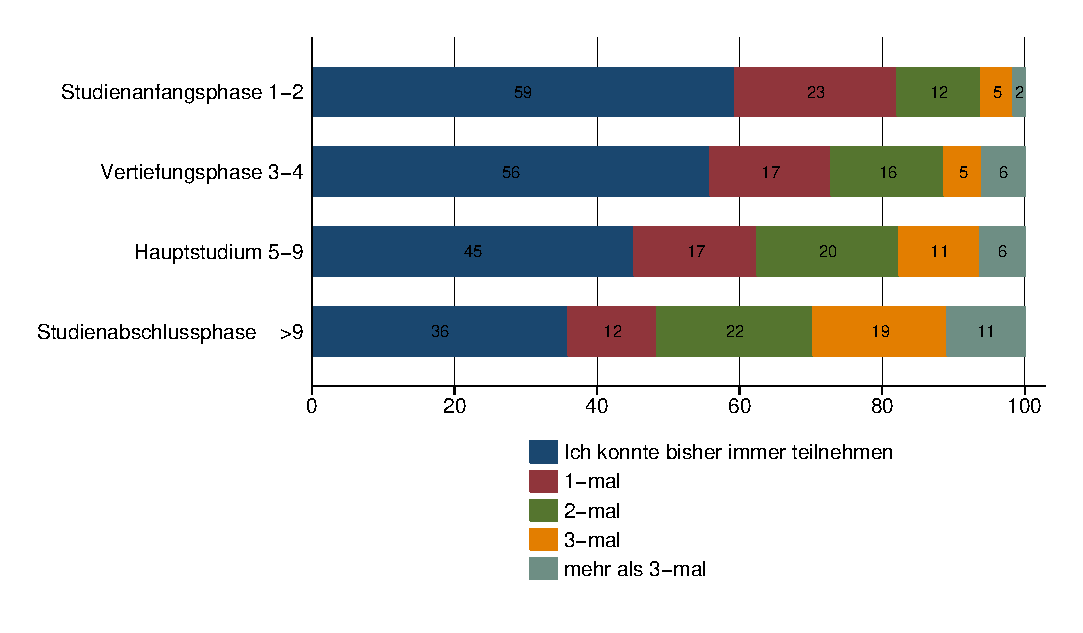
\includegraphics[
%  defaultresolution=72 !,
%  bmpsizefast=false
%]{image}
%\end{verbatim}
% \end{quote}
%
% \subsubsection{Hints}
%
% \begin{itemize}
% \item My version of \xfile{dvips.def} 1999/02/16 v3.0i defines
%       rules for the supported bitmap extensions, but does not
%       include them in the list of extensions that are tried
%       if the file name is not given with an extension.
%       In such a case, the list of extensions can be set
%       by \cs{DeclareGraphicsExtensions}, see \xpackage{grfguide}.
%       The following code just extends the list:
%       \begin{quote}
%\begin{verbatim}
%\makeatletter
%\g@addto@macro\Gin@extensions{,.bmp,.pcx,.msp}
%\makeatother
%\end{verbatim}
%       \end{quote}
% \item My version of \xfile{dvipdfm.def} 1998/11/24 vx.x misses
%       the graphics rule for PNG files. It can be added by:
%       \begin{quote}
%\begin{verbatim}
%\DeclareGraphicsRule{.png}{bmp}{.bb}{#1}
%\end{verbatim}
%       \end{quote}
%       See the previous issue to add the extension \xfile{.png} to the list
%       of extensions for package \xpackage{graphics}.
% \end{itemize}
%
% \subsubsection{Test program}
%
% There is a test program \xfile{bmpsize-test.tex}. Run it through
% \verb|latex|, \verb|pdflatex|, or \verb|pdftex|. Then given
% image files are inspected and the result is printed.
%
% \subsubsection{Interface for programmers}
%
% The macro names of the parsers are \verb|\bmpsize@read@|\meta{type}.
% Example: \cs{bmpsize@read@jpg} in case of JPEG.
%
% A parser sets the switch \cs{ifbmpsize@ok} to true, if it
% could successfully parse the image file.
% The width and height are returnd in \cs{bmpsize@width} and
% \cs{bmpsize@height}. If information about density is available,
% it is used to calculate width and height of the image, otherwise
% the values given by option \xoption{defaultresolution} is used.
% \xoption{resolution} overwrites the values in the image file.
%
% \subsection{Improved bitmap inclusion}
%
% Some drivers for package \xpackage{graphics} define the graphics
% type \xoption{bmp} for bitmap images. The code in the standard
% drivers for \xoption{dvips}, \xoption{dvipdfm}, and \xoption{dvipdfmx}
% is very basic and misses essential features of the
% package \xpackage{graphicx}. Therefore the code for bitmap
% inclusion is automatically rewritten by this package to add
% the following features:
% \begin{itemize}
% \item Support for \xoption{viewport} and \xoption{trim}.
% \item Support for \xoption{clip}.
% \item In case of \xoption{dvipdfm} and \xoption{dvipdfmx} the
%       bitmap images are reused and not included again if they
%       are used more than once.
% \end{itemize}
% However, there is a difference between \xoption{dvipdfm} and
% \xoption{dvipdfmx}, especially if images are reused. In the
% former case the reused box has width and height of 1bp, in the
% latter case its natural width. Thus the correct driver option must be given.
% \xoption{dvipdfm} and \xoption{dvipdfmx} are not equivalent.
%
% Older versions of \xoption{dvipdfmx} uses a size of 1in. However I do
% want to distinguish between versions of the same program. Therefore the
% support of these older versions has stopped with version 1.6 of this package.
% Use version dvipdfmx-20090708 or newer (some few versions before will
% probably also work, but I don't want to investigate this further).
%
% \StopEventually{
% }
%
% \section{Implementation}
%
% \subsection{Basic package \xpackage{bmpsize-base}}
%
%    Identification.
%    \begin{macrocode}
%<*base>
\ProvidesPackage{bmpsize-base}%
  [2009/09/04 v1.6 Basic part of bmpsize (HO)]%
%    \end{macrocode}
%    Modules of package \xpackage{fp} are used for calculations.
%    \begin{macrocode}
\RequirePackage{fp-basic}
\RequirePackage{fp-snap}
%    \end{macrocode}
%    Package \xpackage{fp} uses nested \cs{loop} structures.
%    That breaks with the plain-\TeX\ version of \cs{loop}.
%    Therefore we use the \LaTeX\ variant.
%    \begin{macro}{\@bmpsize@plain@loop}
%    \begin{macrocode}
\long\def\@bmpsize@plain@loop#1\repeat{%
  \def\iterate{%
    #1\relax
    \expandafter\iterate\fi
  }%
  \iterate
  \let\iterate\relax
}
%    \end{macrocode}
%    \end{macro}
%    \begin{macrocode}
\RequirePackage{pdftexcmds}[2007/11/11]
%    \end{macrocode}
%    \begin{macrocode}
\newif\ifbmpsize@ok
\let\@bmpsize@ok\bmpsize@oktrue

\newif\if@bmpsize@bigendian
\newif\if@bmpsize@absnum
\newif\if@bmpsize@user@resolution
\newif\if@bmpsize@fast
\@bmpsize@fasttrue

\def\@bmpsize@init{%
  \let\@bmpsize@org@plain@loop\loop
  \let\loop\@bmpsize@plain@loop
  \bmpsize@okfalse
  \@bmpsize@bigendiantrue
  \@bmpsize@absnumfalse
  \let\bmpsize@pixelwidth\relax
  \let\bmpsize@pixelheight\relax
  \let\bmpsize@pixelx\relax
  \let\bmpsize@pixely\relax
  \let\bmpsize@unit\relax
  \let\bmpsize@pixelxdenom\relax
  \let\bmpsize@pixelydenom\relax
  \let\bmpsize@orientation\relax
}

\def\@bmpsize@stop#1\@nil{}

\def\@bmpsize@loop#1{%
  #1%
  \@bmpsize@loop{#1}%
}
\def\@bmpsize@break#1\@bmpsize@loop#2{}

\def\@bmpsize@size#1#2#3{%
  \edef#3{\pdf@filesize{#1}}%
  \ifx#3\@empty
    \expandafter\@bmpsize@stop
  \fi
  \ifnum#3<#2\relax
    \expandafter\@bmpsize@stop
  \fi
}

\def\@bmpsize@read#1#2#3{%
  \edef\@bmpsize@buf{\pdf@filedump{#3}{#2}{#1}}%
  \edef\@bmpsize@temp{%
    \noexpand\@bmpsize@check@byte{#2}\@bmpsize@buf{}{}\noexpand\\%
  }%
  \@bmpsize@temp
}
\def\@bmpsize@fillbuf#1{%
  \ifx\@bmpsize@buf\@empty
    \expandafter\@firstofone
  \else
    \expandafter\@gobble
  \fi
  {%
    \edef\@bmpsize@buf{%
      \pdf@filedump{\bmpsize@offset}{\bmpsize@fillbuflength}{#1}%
    }%
    \ifx\@bmpsize@buf\@empty
      \expandafter\@bmpsize@stop
    \fi
    \edef\bmpsize@offset{\the\numexpr\bmpsize@offset+\bmpsize@fillbuflength}%
  }%
}
\def\bmpsize@fillbuflength{10}

\def\@bmpsize@append#1#2#3{%
  \edef#1{#2#3}%
}
\def\@bmpsize@pushback#1{%
  \edef\@bmpsize@buf{#1\@bmpsize@buf}%
}

\def\@bmpsize@iswhite#1{%
  \ifnum\pdf@strcmp{#1}{09}=\z@
  \else
    \ifnum\pdf@strcmp{#1}{0A}=\z@
    \else
      \ifnum\pdf@strcmp{#1}{0D}=\z@
      \else
        \ifnum\pdf@strcmp{#1}{20}=\z@
        \else
          1%
        \fi
      \fi
    \fi
  \fi
  \space
}
\def\@bmpsize@isdigit#1{%
  \ifnum\pdf@strcmp{#1}{30}<\z@
    1%
  \else
    \ifnum\pdf@strcmp{#1}{39}>\z@
      1%
    \fi
  \fi
  \space
}

\def\@bmpsize@check@byte#1#2#3{%
  \ifnum#1<\@ne
    \csname fi\endcsname
    \@bmpsize@cleanup@end
  \else
    \csname fi\endcsname
  \ifx!#2#3!%
    \csname fi\endcsname
    \@bmpsize@stop
  \else
    \csname fi\endcsname
    \expandafter\@bmpsize@check@byte\expandafter{\the\numexpr#1-1}%
}
\def\@bmpsize@cleanup@end#1\\{}

\def\@bmpsize@swap@maybe#1{%
  \if@bmpsize@bigendian
  \else
    \edef#1{\expandafter\@bmpsize@@swap#1\@empty\@empty\@empty\@empty}%
  \fi
}
\def\@bmpsize@@swap#1#2#3#4#5#6#7#8{%
  #7#8#5#6#3#4#1#2%
}

\def\@bmpsize@skip@one{%
  \edef\@bmpsize@buf{\expandafter\@gobbletwo\@bmpsize@buf}%
}
\def\@bmpsize@skip@two{%
  \edef\@bmpsize@buf{\expandafter\@gobblefour\@bmpsize@buf}%
}
\def\@bmpsize@skip@four{%
  \edef\@bmpsize@buf{%
    \expandafter\expandafter\expandafter\@gobblefour\expandafter
    \@gobblefour\@bmpsize@buf
  }%
}

\def\@bmpsize@grab#1#2{%
  \edef#1{\noexpand\@bmpsize@grab@byte#2=\@bmpsize@buf\noexpand\\}%
  \edef#1{#1}%
}
\def\@bmpsize@grab@byte#1=#2#3{%
  #2#3%
  \ifnum#1>\@ne
    \expandafter\@bmpsize@grab@byte\the\numexpr#1-1\expandafter=%
  \else
    \expandafter\@bmpsize@cleanup@end
  \fi
}

\def\@bmpsize@abs@maybe#1{%
  \let\@bmpsize@temp\relax
  \if@bmpsize@absnum
    \ifnum"\expandafter\@car#1\@nil>7 %
      \edef#1{\expandafter\@bmpsize@abs@byte#1\relax}%
      \ifnum\pdf@strcmp{#1}{7FFFFFFF}=\z@
        \let\@bmpsize@temp\@bmpsize@stop
      \else
        \def\@bmpsize@temp{\edef#1{\the\numexpr#1+1}}%
      \fi
    \fi
  \fi
}
\def\@bmpsize@abs@byte#1{%
  \ifx#1\relax
  \else
    \ifcase"0#1 %
      F\or E\or D\or C\or B\or A\or 9\or 8\or
      7\or 6\or 5\or 4\or 3\or 2\or 1\or 0%
    \fi
    \expandafter\@bmpsize@abs@byte
  \fi
}

\def\@bmpsize@num@one#1{%
  \@bmpsize@grab#11%
  \@bmpsize@abs@maybe#1%
  \edef#1{\number"#1}%
  \@bmpsize@temp
  \@bmpsize@skip@one
}
\def\@bmpsize@num@two#1{%
  \@bmpsize@grab#12%
  \@bmpsize@swap@maybe#1%
  \@bmpsize@abs@maybe#1%
  \edef#1{\number"#1}%
  \@bmpsize@temp
  \@bmpsize@skip@two
}
\def\@bmpsize@num@four#1{%
  \@bmpsize@grab#14%
  \@bmpsize@swap@maybe#1%
  \@bmpsize@abs@maybe#1%
  \ifnum\pdf@strcmp{#1}{7FFFFFFF}>\z@
    \expandafter\@bmpsize@stop
  \fi
  \edef#1{\number"#1}%
  \@bmpsize@temp
  \@bmpsize@skip@four
}

\def\@bmpsize@div#1#2#3{% #1 := #2/#3
  \FPdiv#1{#2}{#3}%
  \@bmpsize@beautify#1%
}
\def\@bmpsize@beautify#1{%
  \FPifint#1%
    \edef#1{\expandafter\@bmpsize@trunc#1.\@nil}%
  \else
    \edef#1{\expandafter\@bmpsize@cleanup@frac#1.\@nil}%
  \fi
}
\def\@bmpsize@trunc#1.#2\@nil{#1}
% #1 isn't an integer, thus we should have at least one
% necessary digit after the dot
\def\@bmpsize@cleanup@frac#1.#2#3.#4\@nil{%
  #1.#2%
  \ifx\\#3\\%
  \else
    \@bmpsize@cleanup@fracdigits#3000000000\@nil
  \fi
}
\def\@bmpsize@cleanup@fracdigits#1#2#3#4#5#6#7#8#9{%
  \ifcase#9 %
    \ifcase#8 %
      \ifcase#7 %
        \ifcase#6 %
          \ifcase#5 %
            \ifcase #4 %
              \ifcase #3 %
                \ifcase #2 %
                  \ifcase #1 %
                  \else
                    #1%
                  \fi
                \else
                  #1#2%
                \fi
              \else
                #1#2#3%
              \fi
            \else
              #1#2#3#4%
            \fi
          \else
            #1#2#3#4#5%
          \fi
        \else
          #1#2#3#4#5#6%
        \fi
      \else
        #1#2#3#4#5#6#7%
      \fi
    \else
      #1#2#3#4#5#6#7#8%
    \fi
  \else
    #1#2#3#4#5#6#7#8#9%
  \fi
  \@bmpsize@trunc.%
}

\def\@bmpsize@end{%
  \ifbmpsize@ok
    \ifx\bmpsize@pixelwidth\relax
      \bmpsize@okfalse
    \fi
    \ifx\bmpsize@pixelheight\relax
      \bmpsize@okfalse
    \fi
  \fi
  \ifbmpsize@ok
    \ifnum\bmpsize@pixelwidth>\z@
    \else
      \bmpsize@okfalse
    \fi
    \ifnum\bmpsize@pixelheight>\z@
    \else
      \bmpsize@okfalse
    \fi
  \fi
  \ifbmpsize@ok
    \ifcase 0%
      \ifx\bmpsize@pixelx\relax 1 \fi
      \ifx\bmpsize@pixely\relax 1 \fi
      \ifnum\bmpsize@pixelx>\z@\else 1 \fi
      \ifnum\bmpsize@pixely>\z@\else 1 \fi
      \ifx\bmpsize@pixelxdenom\relax
         \ifx\bmpsize@pixelydenom\relax\else 1 \fi
      \else
        \ifnum\bmpsize@pixelxdenom>\z@\else 1 \fi
      \fi
      \ifx\bmpsize@pixelydenom\relax
      \else
        \ifnum\bmpsize@pixelydenom>\z@\else 1 \fi
      \fi
    \else
      \let\bmpsize@pixelx\relax
      \let\bmpsize@pixely\relax
      \let\bmpsize@unit\relax
      \let\bmpsize@pixelxdenom\relax
      \let\bmpsize@pixelydenom\relax
    \fi
    \ifx\bmpsize@pixelxdenom\relax
    \else
      \@bmpsize@div\bmpsize@pixelx\bmpsize@pixelx\bmpsize@pixelxdenom
      \@bmpsize@div\bmpsize@pixely\bmpsize@pixely\bmpsize@pixelydenom
      \let\bmpsize@pixelxdenom\relax
      \let\bmpsize@pixelydenom\relax
    \fi
    \ifcase 0\ifx\bmpsize@unit\relax 1\fi
             \if@bmpsize@user@resolution 1\fi
             \relax
      \let\bmpsize@calc@unit\bmpsize@unit
      \let\bmpsize@calc@pixelx\bmpsize@pixelx
      \let\bmpsize@calc@pixely\bmpsize@pixely
    \else
      \let\bmpsize@calc@unit\bmpsize@unit@default
      \let\bmpsize@calc@pixelx\bmpsize@pixelx@default
      \let\bmpsize@calc@pixely\bmpsize@pixely@default
      \ifx\bmpsize@calc@pixely\Gin@exclamation
        \ifx\bmpsize@pixelx\relax
          \let\bmpsize@calc@pixely\bmpsize@calc@pixelx
        \else
          \FPdiv\bmpsize@calc@pixely\bmpsize@calc@pixelx\bmpsize@pixelx
          \FPmul\bmpsize@calc@pixely\bmpsize@calc@pixely\bmpsize@pixely
        \fi
      \else
        \ifx\bmpsize@calc@pixelx\Gin@exclamation
          \ifx\bmpsize@pixelx\relax
            \let\bmpsize@calc@pixelx\bmpsize@calc@pixely
          \else
            \FPdiv\bmpsize@calc@pixelx\bmpsize@calc@pixely\bmpsize@pixely
            \FPmul\bmpsize@calc@pixelx\bmpsize@calc@pixelx\bmpsize@pixelx
          \fi
        \fi
      \fi
    \fi
    \FPdiv\bmpsize@width\bmpsize@pixelwidth\bmpsize@calc@pixelx
    \FPdiv\bmpsize@height\bmpsize@pixelheight\bmpsize@calc@pixely
    % calculation of width and height in bp for package graphics
    % 1in = 72bp = 72.27pt, 72/72.27 = 8/8.03, 1pt = 65536sp
    \if@bmpsize@fast
      \edef\bmpsize@width{%
        \strip@pt\dimexpr.99626\dimexpr
        \bmpsize@width\dimexpr\bmpsize@calc@unit
      }%
      \edef\bmpsize@height{%
        \strip@pt\dimexpr.99626\dimexpr
        \bmpsize@height\dimexpr\bmpsize@calc@unit
      }%
    \else
      \edef\@bmpsize@temp{\number\dimexpr\bmpsize@calc@unit}%
      \ifnum\@bmpsize@temp>100000 %
        \FPmul\@bmpsize@temp\@bmpsize@temp{0.00001}%
        \def\@bmpsize@corr{100000}%
      \else
        \let\@bmpsize@corr\relax
      \fi
      \FPmul\bmpsize@width\bmpsize@width\@bmpsize@temp
      \FPmul\bmpsize@height\bmpsize@height\@bmpsize@temp
      \FPmul\bmpsize@width\bmpsize@width{8}%
      \FPmul\bmpsize@height\bmpsize@height{8}%
      \FPdiv\bmpsize@width\bmpsize@width{8.03}%
      \FPdiv\bmpsize@height\bmpsize@height{8.03}%
      \FPdiv\bmpsize@width\bmpsize@width{65536}%
      \FPdiv\bmpsize@height\bmpsize@height{65536}%
      \ifx\@bmpsize@corr\relax
      \else
        \FPmul\bmpsize@width\bmpsize@width\@bmpsize@corr
        \FPmul\bmpsize@height\bmpsize@height\@bmpsize@corr
      \fi
      \FPround\bmpsize@width\bmpsize@width{5}%
      \FPround\bmpsize@height\bmpsize@height{5}%
      \@bmpsize@beautify\bmpsize@width
      \@bmpsize@beautify\bmpsize@height
    \fi
  \fi
  \let\loop\@bmpsize@org@plain@loop
}
\def\bmpsize@unit@default{72.27pt}% more accurate than 1in
\def\bmpsize@pixelx@default{72}
\let\bmpsize@pixely@default\Gin@exclamation

\def\bmpsize@types{png,jpg,bmp,gif,tiff,pnm,pam,xpm,tga,pcx,msp,sgi}
%</base>
%    \end{macrocode}
%
% \subsection{Bitmap formats}
%
% \subsubsection{png}
%
%\iffalse
%<*ignore>
%\fi
%\begin{verbatim}
%begin png
%big-endian
%
%read 24 0
%grab 8        -> $temp
%check streq $temp [0x89 "PNG" 0x0D 0x0A 0x1A 0x0A]
%num 4         -> $length
%grab 4        -> $temp
%check streq $temp ["IHDR"]
%num 4         -> $pixelwidth
%num 4         -> $pixelheight
%ok
%assign numexpr(20 + $length) -> $offset
%loop
%  read 8 $offset
%  num 4       -> $length
%  grab 4      -> $temp
%  if streq $temp ["IDAT"]
%    stop
%  fi
%  if streq $temp ["pHYs"]
%    read 9 numexpr($offset + 8)
%    num 4     -> $pixelx
%    num 4     -> $pixely
%    grab 1     -> $temp
%    if numeq $temp 1
%      assign {100cm} -> $unit
%    fi
%    stop
%  fi
%  assign numexpr($offset + 12 + $length) -> $offset
%repeat
%end
%\end{verbatim}
%\iffalse
%</ignore>
%\fi
%    \begin{macro}{\bmpsize@read@png}
%    \begin{macrocode}
%<*base>
\def\bmpsize@read@png#1{%
  \@bmpsize@init
  \@bmpsize@bigendiantrue
  \@bmpsize@read{#1}{24}{0}%
  \@bmpsize@grab\bmpsize@temp{8}%
  \@bmpsize@skip@four
  \@bmpsize@skip@four
  \ifnum\pdf@strcmp{\bmpsize@temp}{89504E470D0A1A0A}=\z@
  \else
    \expandafter\@bmpsize@stop
  \fi
  \@bmpsize@num@four\bmpsize@length
  \@bmpsize@grab\bmpsize@temp{4}%
  \@bmpsize@skip@four
  \ifnum\pdf@strcmp{\bmpsize@temp}{49484452}=\z@
  \else
    \expandafter\@bmpsize@stop
  \fi
  \@bmpsize@num@four\bmpsize@pixelwidth
  \@bmpsize@num@four\bmpsize@pixelheight
  \@bmpsize@ok
  \edef\bmpsize@offset{\the\numexpr20+\bmpsize@length}%
  \@bmpsize@loop{%
    \@bmpsize@read{#1}{8}{\bmpsize@offset}%
    \@bmpsize@num@four\bmpsize@length
    \@bmpsize@grab\bmpsize@temp{4}%
    \@bmpsize@skip@four
    \ifnum\pdf@strcmp{\bmpsize@temp}{49444154}=\z@
      \expandafter\@firstofone
    \else
      \expandafter\@gobble
    \fi
    {%
      \@bmpsize@stop
    }%
    \ifnum\pdf@strcmp{\bmpsize@temp}{70485973}=\z@
      \expandafter\@firstofone
    \else
      \expandafter\@gobble
    \fi
    {%
      \@bmpsize@read{#1}{9}{\numexpr\bmpsize@offset+8\relax}%
      \@bmpsize@num@four\bmpsize@pixelx
      \@bmpsize@num@four\bmpsize@pixely
      \@bmpsize@grab\bmpsize@temp{1}%
      \@bmpsize@skip@one
      \ifnum\bmpsize@temp=1\relax
        \expandafter\@firstofone
      \else
        \expandafter\@gobble
      \fi
      {%
        \def\bmpsize@unit{100cm}%
      }%
      \@bmpsize@stop
    }%
    \edef\bmpsize@offset{\the\numexpr\bmpsize@offset+12+\bmpsize@length}%
  }%
  \@bmpsize@stop
  \@nil
  \@bmpsize@end
}%
%</base>
%    \end{macrocode}
%    \end{macro}
%
% \subsubsection{jpg}
%
%\iffalse
%<*ignore>
%\fi
%\begin{verbatim}
%begin jpg
%
%read 3 0
%grab 3      -> $temp % SOI and 0xFF
%check streq $temp [0xFF 0xD8 0xFF]
%assign {2} -> $offset
%assign {0} -> $exifdensity
%loop
%  read 4 $offset
%  grab 1    -> $temp
%  check streq $temp [0xFF]
%  num 1    -> $temp
%  if numeq $temp 0xDA % SOS
%    stop
%  fi
%  % look for JFIF APP0 segment
%  if numeq $temp 0xE0 % APP0
%    num 2       -> $length
%    if numeq $exifdensity 0
%      if numge $length 16 % a JFIF segment has 16 bytes at least
%        read 12 numexpr($offset + 4)
%        grab 5      -> $temp % identifier
%        if streq $temp ["JFIF" 0x0]
%          check numge $length 16
%          skip 2 % version
%          num 1       -> $temp % units
%          if numeq $temp 1
%            assign {72.27pt} -> $unit
%          else
%            if numeq $temp 2
%              assign {1cm} -> $unit
%            fi
%          fi
%          num 2    -> $pixelx
%          num 2    -> $pixely
%        fi
%      fi
%    fi
%  else
%    if numeq $temp 0xE1 % APP1
%      % look for Exif APP1 segment
%      num 2 -> $length
%      if numge $length 20 % identifier (6) + Tiff header (8) + first IFD (>=6)
%        read 20 numexpr($offset + 4)
%        grab 6 -> $temp
%        if streq $temp ["Exif" 0x0 0x0]
%          assign numexpr($offset + 10) -> $exifoffset
%          % read TIFF header
%          grab 2 -> $temp
%          if streq $temp ["II"]
%            little-endian
%          else
%            check streq $temp ["MM"]
%            % big-endian
%          fi
%          num 2 -> $temp
%          check numeq $temp 42
%          num 4 -> $temp % offset of first IFD
%          check numgt $temp 0
%          % read first IFD
%          assign numexpr($temp + $exifoffset) -> $off
%          read 2 $off
%          num 2 -> $entries
%          assign numexpr($off + 2) -> $off
%          loop
%            if numeq $entries 0
%              break
%            fi
%            assign numexpr($entries - 1) -> $entries
%            % entry format:
%            % 2 tag
%            % 2 field type
%            % 4 count
%            % 4 value/offset
%            read 12 $off
%            assign numexpr($off + 12) -> $off
%            num 2 -> $tag
%            if numeq $tag 296 % ResolutionUnit
%              skip 6 % type: 3 (short), count: 1
%              num 2 -> $temp
%              ifcase $temp
%              or % 1
%                clear $unit
%              or % 2
%                assign {72.27pt} -> $unit
%              or % 3
%                assign {1cm} -> $unit
%              else
%                clear $unit % unknown
%              fi
%              ifcase $temp
%              or % 1
%              or % 2
%                assign {1} -> $exifdensity
%              or % 3
%                assign {1} -> $exifdensity
%              else
%                assign $exifdensity -> $exifdensity
%              fi
%            fi
%            % 256 ImageWidth (use width of JPG part)
%            % 257 ImageHeight (use height of JPG part)
%            if numeq $tag 274 % Orientation
%              skip 6 % type: 3 (short), count: 1
%              num 2 -> $temp
%              if numge $temp 0 
%                if numle $temp 8
%                  assign $temp -> $orientation
%                fi
%              fi
%            fi
%            if numeq $tag 282 % XResolution
%              skip 6
%              num 4 -> $temp
%              read 8 numexpr($temp + $exifoffset)
%              num 4 -> $pixelx
%              num 4 -> $temp
%              if numeq $temp 1
%              else
%                assign numexpr($temp) -> $pixelxdenom
%                % div $pixelx $temp -> $pixelx
%              fi
%            fi
%            if numeq $tag 283 % YResolution
%              skip 6
%              num 4 -> $temp
%              read 8 numexpr($temp + $exifoffset)
%              num 4 -> $pixely
%              num 4 -> $temp
%              if numeq $temp 1
%              else
%                assign numexpr($temp) -> $pixelydenom
%                % div $pixely $temp -> $pixely
%              fi
%            fi
%          repeat
%          big-endian
%        fi
%      fi
%    else
%      assign numexpr($temp - 0xC0) -> $temp
%      ifcase $temp % SOF_0
%      or % SOF_1
%      or % SOF_2
%      or % SOF_3
%      or % DHT
%        assign {-1} -> $temp
%      or % SOF_5
%      or % SOF_6
%      or % SOF_7
%      or % JPG
%        assign {-1} -> $temp
%      or % SOF_9
%      or % SOF_10
%      or % SOF_11
%      or % DAC
%        assign {-1} -> $temp
%      or % SOF_13
%      or % SOF_14
%      or % SOF_15
%      else
%        assign {-1} -> $temp
%      fi
%      if numeq $temp -1
%      else
%        read 4 numexpr($offset + 5)
%        num 2  -> $pixelheight
%        num 2  -> $pixelwidth
%        if numeq $pixelheight 0
%          clear $pixelheight
%          stop
%        fi
%        ok
%        stop
%      fi
%      num 2 -> $length
%    fi
%  fi
%  assign numexpr($offset + $length + 2) -> $offset
%repeat
%end
%\end{verbatim}
%\iffalse
%</ignore>
%\fi
%    \begin{macro}{\bmpsize@read@jpg}
%    \begin{macrocode}
%<*base>
\def\bmpsize@read@jpg#1{%
  \@bmpsize@init
  \@bmpsize@read{#1}{3}{0}%
  \@bmpsize@grab\bmpsize@temp{3}%
  \@bmpsize@skip@two
  \@bmpsize@skip@one
  \ifnum\pdf@strcmp{\bmpsize@temp}{FFD8FF}=\z@
  \else
    \expandafter\@bmpsize@stop
  \fi
  \def\bmpsize@offset{2}%
  \def\bmpsize@exifdensity{0}%
  \@bmpsize@loop{%
    \@bmpsize@read{#1}{4}{\bmpsize@offset}%
    \@bmpsize@grab\bmpsize@temp{1}%
    \@bmpsize@skip@one
    \ifnum\pdf@strcmp{\bmpsize@temp}{FF}=\z@
    \else
      \expandafter\@bmpsize@stop
    \fi
    \@bmpsize@num@one\bmpsize@temp
    \ifnum\bmpsize@temp=218\relax
      \expandafter\@firstofone
    \else
      \expandafter\@gobble
    \fi
    {%
      \@bmpsize@stop
    }%
    \ifnum\bmpsize@temp=224\relax
      \expandafter\@firstoftwo
    \else
      \expandafter\@secondoftwo
    \fi
    {%
      \@bmpsize@num@two\bmpsize@length
      \ifnum\bmpsize@exifdensity=0\relax
        \expandafter\@firstofone
      \else
        \expandafter\@gobble
      \fi
      {%
        \unless\ifnum\bmpsize@length<16\relax
          \expandafter\@firstofone
        \else
          \expandafter\@gobble
        \fi
        {%
          \@bmpsize@read{#1}{12}{\numexpr\bmpsize@offset+4\relax}%
          \@bmpsize@grab\bmpsize@temp{5}%
          \@bmpsize@skip@four
          \@bmpsize@skip@one
          \ifnum\pdf@strcmp{\bmpsize@temp}{4A46494600}=\z@
            \expandafter\@firstofone
          \else
            \expandafter\@gobble
          \fi
          {%
            \ifnum\bmpsize@length<16\relax
              \expandafter\@bmpsize@stop
            \fi
            \@bmpsize@skip@two
            \@bmpsize@num@one\bmpsize@temp
            \ifnum\bmpsize@temp=1\relax
              \expandafter\@firstoftwo
            \else
              \expandafter\@secondoftwo
            \fi
            {%
              \def\bmpsize@unit{72.27pt}%
            }{%
              \ifnum\bmpsize@temp=2\relax
                \expandafter\@firstofone
              \else
                \expandafter\@gobble
              \fi
              {%
                \def\bmpsize@unit{1cm}%
              }%
            }%
            \@bmpsize@num@two\bmpsize@pixelx
            \@bmpsize@num@two\bmpsize@pixely
          }%
        }%
      }%
    }{%
      \ifnum\bmpsize@temp=225\relax
        \expandafter\@firstoftwo
      \else
        \expandafter\@secondoftwo
      \fi
      {%
        \@bmpsize@num@two\bmpsize@length
        \unless\ifnum\bmpsize@length<20\relax
          \expandafter\@firstofone
        \else
          \expandafter\@gobble
        \fi
        {%
          \@bmpsize@read{#1}{20}{\numexpr\bmpsize@offset+4\relax}%
          \@bmpsize@grab\bmpsize@temp{6}%
          \@bmpsize@skip@four
          \@bmpsize@skip@two
          \ifnum\pdf@strcmp{\bmpsize@temp}{457869660000}=\z@
            \expandafter\@firstofone
          \else
            \expandafter\@gobble
          \fi
          {%
            \edef\bmpsize@exifoffset{\the\numexpr\bmpsize@offset+10}%
            \@bmpsize@grab\bmpsize@temp{2}%
            \@bmpsize@skip@two
            \ifnum\pdf@strcmp{\bmpsize@temp}{4949}=\z@
              \expandafter\@firstoftwo
            \else
              \expandafter\@secondoftwo
            \fi
            {%
              \@bmpsize@bigendianfalse
            }{%
              \ifnum\pdf@strcmp{\bmpsize@temp}{4D4D}=\z@
              \else
                \expandafter\@bmpsize@stop
              \fi
            }%
            \@bmpsize@num@two\bmpsize@temp
            \ifnum\bmpsize@temp=42\relax
            \else
              \expandafter\@bmpsize@stop
            \fi
            \@bmpsize@num@four\bmpsize@temp
            \ifnum\bmpsize@temp>0\relax
            \else
              \expandafter\@bmpsize@stop
            \fi
            \edef\bmpsize@off{\the\numexpr\bmpsize@temp+\bmpsize@exifoffset}%
            \@bmpsize@read{#1}{2}{\bmpsize@off}%
            \@bmpsize@num@two\bmpsize@entries
            \edef\bmpsize@off{\the\numexpr\bmpsize@off+2}%
            \@bmpsize@loop{%
              \ifnum\bmpsize@entries=0\relax
                \expandafter\@firstofone
              \else
                \expandafter\@gobble
              \fi
              {%
                \@bmpsize@break
              }%
              \edef\bmpsize@entries{\the\numexpr\bmpsize@entries-1}%
              \@bmpsize@read{#1}{12}{\bmpsize@off}%
              \edef\bmpsize@off{\the\numexpr\bmpsize@off+12}%
              \@bmpsize@num@two\bmpsize@tag
              \ifnum\bmpsize@tag=296\relax
                \expandafter\@firstofone
              \else
                \expandafter\@gobble
              \fi
              {%
                \@bmpsize@skip@four
                \@bmpsize@skip@two
                \@bmpsize@num@two\bmpsize@temp
                \ifcase\bmpsize@temp\relax
                \or
                  \let\bmpsize@unit\relax
                \or
                  \def\bmpsize@unit{72.27pt}%
                \or
                  \def\bmpsize@unit{1cm}%
                \else
                  \let\bmpsize@unit\relax
                \fi
                \ifcase\bmpsize@temp\relax
                \or
                \or
                  \def\bmpsize@exifdensity{1}%
                \or
                  \def\bmpsize@exifdensity{1}%
                \else
                  \let\bmpsize@exifdensity\bmpsize@exifdensity
                \fi
              }%
              \ifnum\bmpsize@tag=274\relax
                \expandafter\@firstofone
              \else
                \expandafter\@gobble
              \fi
              {%
                \@bmpsize@skip@four
                \@bmpsize@skip@two
                \@bmpsize@num@two\bmpsize@temp
                \unless\ifnum\bmpsize@temp<0\relax
                  \expandafter\@firstofone
                \else
                  \expandafter\@gobble
                \fi
                {%
                  \unless\ifnum\bmpsize@temp>8\relax
                    \expandafter\@firstofone
                  \else
                    \expandafter\@gobble
                  \fi
                  {%
                    \let\bmpsize@orientation\bmpsize@temp
                  }%
                }%
              }%
              \ifnum\bmpsize@tag=282\relax
                \expandafter\@firstofone
              \else
                \expandafter\@gobble
              \fi
              {%
                \@bmpsize@skip@four
                \@bmpsize@skip@two
                \@bmpsize@num@four\bmpsize@temp
                \@bmpsize@read{#1}{8}{\numexpr\bmpsize@temp+\bmpsize@exifoffset\relax}%
                \@bmpsize@num@four\bmpsize@pixelx
                \@bmpsize@num@four\bmpsize@temp
                \ifnum\bmpsize@temp=1\relax
                  \expandafter\@gobble
                \else
                  \expandafter\@firstofone
                \fi
                {%
                  \edef\bmpsize@pixelxdenom{\the\numexpr\bmpsize@temp}%
                }%
              }%
              \ifnum\bmpsize@tag=283\relax
                \expandafter\@firstofone
              \else
                \expandafter\@gobble
              \fi
              {%
                \@bmpsize@skip@four
                \@bmpsize@skip@two
                \@bmpsize@num@four\bmpsize@temp
                \@bmpsize@read{#1}{8}{\numexpr\bmpsize@temp+\bmpsize@exifoffset\relax}%
                \@bmpsize@num@four\bmpsize@pixely
                \@bmpsize@num@four\bmpsize@temp
                \ifnum\bmpsize@temp=1\relax
                  \expandafter\@gobble
                \else
                  \expandafter\@firstofone
                \fi
                {%
                  \edef\bmpsize@pixelydenom{\the\numexpr\bmpsize@temp}%
                }%
              }%
            }%
            \@bmpsize@bigendiantrue
          }%
        }%
      }{%
        \edef\bmpsize@temp{\the\numexpr\bmpsize@temp-192}%
        \ifcase\bmpsize@temp\relax
        \or
        \or
        \or
        \or
          \def\bmpsize@temp{-1}%
        \or
        \or
        \or
        \or
          \def\bmpsize@temp{-1}%
        \or
        \or
        \or
        \or
          \def\bmpsize@temp{-1}%
        \or
        \or
        \or
        \else
          \def\bmpsize@temp{-1}%
        \fi
        \ifnum\bmpsize@temp=-1\relax
          \expandafter\@gobble
        \else
          \expandafter\@firstofone
        \fi
        {%
          \@bmpsize@read{#1}{4}{\numexpr\bmpsize@offset+5\relax}%
          \@bmpsize@num@two\bmpsize@pixelheight
          \@bmpsize@num@two\bmpsize@pixelwidth
          \ifnum\bmpsize@pixelheight=0\relax
            \expandafter\@firstofone
          \else
            \expandafter\@gobble
          \fi
          {%
            \let\bmpsize@pixelheight\relax
            \@bmpsize@stop
          }%
          \@bmpsize@ok
          \@bmpsize@stop
        }%
        \@bmpsize@num@two\bmpsize@length
      }%
    }%
    \edef\bmpsize@offset{\the\numexpr\bmpsize@offset+\bmpsize@length+2}%
  }%
  \@bmpsize@stop
  \@nil
  \@bmpsize@end
}%
%</base>
%    \end{macrocode}
%    \end{macro}
%
% \subsubsection{bmp}
%
%\iffalse
%<*ignore>
%\fi
%\begin{verbatim}
%begin bmp
%little-endian
%
%read 26 0
%grab 2 -> $temp
%check streq $temp ["BM"]
%skip 12
%% header size is 4 bytes in V3+, unknown for V1, V2,
%% known header sizes fit in 2 bytes
%num 2   -> $temp
%if numeq $temp 12 % V1
%  skip 2
%  num 2 -> $pixelwidth
%  num 2 -> $pixelheight
%  % no resolution entries
%  ok
%  stop
%fi
%if numeq $temp 64 % V2
%  skip 2
%  num 2 -> $pixelwidth
%  num 2 -> $pixelheight
%  % missing specification for resolution
%  ok
%  stop
%fi
%% V3, V4, V5
%skip 2
%num 4 -> $pixelwidth
%absnum 4 -> $pixelheight
%ok
%read 8 38
%num 4 -> $pixelx
%num 4 -> $pixely
%assign {100cm} -> $unit
%end
%\end{verbatim}
%\iffalse
%</ignore>
%\fi
%    \begin{macro}{\bmpsize@read@bmp}
%    \begin{macrocode}
%<*base>
\def\bmpsize@read@bmp#1{%
  \@bmpsize@init
  \@bmpsize@bigendianfalse
  \@bmpsize@read{#1}{26}{0}%
  \@bmpsize@grab\bmpsize@temp{2}%
  \@bmpsize@skip@two
  \ifnum\pdf@strcmp{\bmpsize@temp}{424D}=\z@
  \else
    \expandafter\@bmpsize@stop
  \fi
  \@bmpsize@skip@four
  \@bmpsize@skip@four
  \@bmpsize@skip@four
  \@bmpsize@num@two\bmpsize@temp
  \ifnum\bmpsize@temp=12\relax
    \expandafter\@firstofone
  \else
    \expandafter\@gobble
  \fi
  {%
    \@bmpsize@skip@two
    \@bmpsize@num@two\bmpsize@pixelwidth
    \@bmpsize@num@two\bmpsize@pixelheight
    \@bmpsize@ok
    \@bmpsize@stop
  }%
  \ifnum\bmpsize@temp=64\relax
    \expandafter\@firstofone
  \else
    \expandafter\@gobble
  \fi
  {%
    \@bmpsize@skip@two
    \@bmpsize@num@two\bmpsize@pixelwidth
    \@bmpsize@num@two\bmpsize@pixelheight
    \@bmpsize@ok
    \@bmpsize@stop
  }%
  \@bmpsize@skip@two
  \@bmpsize@num@four\bmpsize@pixelwidth
  \@bmpsize@absnumtrue
  \@bmpsize@num@four\bmpsize@pixelheight
  \@bmpsize@absnumfalse
  \@bmpsize@ok
  \@bmpsize@read{#1}{8}{38}%
  \@bmpsize@num@four\bmpsize@pixelx
  \@bmpsize@num@four\bmpsize@pixely
  \def\bmpsize@unit{100cm}%
  \@bmpsize@stop
  \@nil
  \@bmpsize@end
}%
%</base>
%    \end{macrocode}
%    \end{macro}
%
% \subsubsection{gif}
%
%\iffalse
%<*ignore>
%\fi
%\begin{verbatim}
%begin gif
%little-endian
%
%% Header
%read 13 0
%grab 3      -> $temp
%check streq $temp ["GIF"]
%skip 3      % version
%
%% Logical Screen Descriptor
%num 2       -> $pixelwidth
%num 2       -> $pixelheight
%skip 2
%num 1       -> $temp % Pixel Aspect Ratio
%if numeq $temp 0
%else
%  assign numexpr($temp + 15) -> $pixelx
%  assign {64}     -> $pixely
%fi
%ok
%end
%\end{verbatim}
%\iffalse
%</ignore>
%\fi
%    \begin{macro}{\bmpsize@read@gif}
%    \begin{macrocode}
%<*base>
\def\bmpsize@read@gif#1{%
  \@bmpsize@init
  \@bmpsize@bigendianfalse
  \@bmpsize@read{#1}{13}{0}%
  \@bmpsize@grab\bmpsize@temp{3}%
  \@bmpsize@skip@two
  \@bmpsize@skip@one
  \ifnum\pdf@strcmp{\bmpsize@temp}{474946}=\z@
  \else
    \expandafter\@bmpsize@stop
  \fi
  \@bmpsize@skip@two
  \@bmpsize@skip@one
  \@bmpsize@num@two\bmpsize@pixelwidth
  \@bmpsize@num@two\bmpsize@pixelheight
  \@bmpsize@skip@two
  \@bmpsize@num@one\bmpsize@temp
  \ifnum\bmpsize@temp=0\relax
    \expandafter\@gobble
  \else
    \expandafter\@firstofone
  \fi
  {%
    \edef\bmpsize@pixelx{\the\numexpr\bmpsize@temp+15}%
    \def\bmpsize@pixely{64}%
  }%
  \@bmpsize@ok
  \@bmpsize@stop
  \@nil
  \@bmpsize@end
}%
%</base>
%    \end{macrocode}
%    \end{macro}
%
% \subsubsection{tiff}
%
%\iffalse
%<*ignore>
%\fi
%\begin{verbatim}
%begin tiff
%% defaults
%assign {72.27pt} -> $unit
%
%% Image File Header
%read 8 0
%grab 2 -> $temp
%if streq $temp ["II"]
%  little-endian
%else
%  check streq $temp ["MM"]
%  big-endian
%fi
%num 2 -> $temp
%check numeq $temp 42
%num 4 -> $offset % first IFD (Image File Directory)
%
%% First IFD
%read 2 $offset
%assign numexpr($offset + 2) -> $offset
%num 2 -> $entries
%ok % must rely on checks at the end
%loop
%  if numeq $entries 0
%    stop
%  fi
%  assign numexpr($entries - 1) -> $entries
%  % entry format:
%  % 2 tag
%  % 2 field type
%  % 4 count
%  % 4 value/offset
%  read 12 $offset
%  assign numexpr($offset + 12) -> $offset
%  num 2 -> $tag % tag
%  if numeq $temp 296 % ResolutionUnit
%    skip 6 % type: 3 (short), count: 1
%    num 2 -> $temp
%    ifcase $temp
%    or % 1
%      clear $unit
%    or % 2
%      assign {72.27pt} -> $unit
%    or % 3
%      assign {1cm} -> $unit
%    else
%      clear $unit
%    fi
%  fi
%  if numeq $tag 256 % ImageWidth
%    skip 6
%    num 4 -> $pixelwidth
%  fi
%  if numeq $tag 257 % ImageLength
%    skip 6
%    num 4 -> $pixelheight
%  fi
%  if numeq $tag 282 % XResolution
%    skip 6
%    num 4 -> $temp
%    read 8 $temp
%    num 4 -> $pixelx
%    num 4 -> $temp
%    if numeq $temp 1
%    else
%      assign numexpr($temp) -> $pixelxdenom
%      % div $pixelx $temp -> $pixelx
%    fi
%  fi
%  if numeq $tag 283 % YResolution
%    skip 6
%    num 4 -> $temp
%    read 8 $temp
%    num 4 -> $pixely
%    num 4 -> $temp
%    if numeq $temp 1
%    else
%      assign numexpr($temp) -> $pixelydenom
%      % div $pixely $temp -> $pixely
%    fi
%  fi
%repeat
%end
%\end{verbatim}
%\iffalse
%</ignore>
%\fi
%    \begin{macro}{\bmpsize@read@tiff}
%    \begin{macrocode}
%<*base>
\def\bmpsize@read@tiff#1{%
  \@bmpsize@init
  \def\bmpsize@unit{72.27pt}%
  \@bmpsize@read{#1}{8}{0}%
  \@bmpsize@grab\bmpsize@temp{2}%
  \@bmpsize@skip@two
  \ifnum\pdf@strcmp{\bmpsize@temp}{4949}=\z@
    \expandafter\@firstoftwo
  \else
    \expandafter\@secondoftwo
  \fi
  {%
    \@bmpsize@bigendianfalse
  }{%
    \ifnum\pdf@strcmp{\bmpsize@temp}{4D4D}=\z@
    \else
      \expandafter\@bmpsize@stop
    \fi
    \@bmpsize@bigendiantrue
  }%
  \@bmpsize@num@two\bmpsize@temp
  \ifnum\bmpsize@temp=42\relax
  \else
    \expandafter\@bmpsize@stop
  \fi
  \@bmpsize@num@four\bmpsize@offset
  \@bmpsize@read{#1}{2}{\bmpsize@offset}%
  \edef\bmpsize@offset{\the\numexpr\bmpsize@offset+2}%
  \@bmpsize@num@two\bmpsize@entries
  \@bmpsize@ok
  \@bmpsize@loop{%
    \ifnum\bmpsize@entries=0\relax
      \expandafter\@firstofone
    \else
      \expandafter\@gobble
    \fi
    {%
      \@bmpsize@stop
    }%
    \edef\bmpsize@entries{\the\numexpr\bmpsize@entries-1}%
    \@bmpsize@read{#1}{12}{\bmpsize@offset}%
    \edef\bmpsize@offset{\the\numexpr\bmpsize@offset+12}%
    \@bmpsize@num@two\bmpsize@tag
    \ifnum\bmpsize@temp=296\relax
      \expandafter\@firstofone
    \else
      \expandafter\@gobble
    \fi
    {%
      \@bmpsize@skip@four
      \@bmpsize@skip@two
      \@bmpsize@num@two\bmpsize@temp
      \ifcase\bmpsize@temp\relax
      \or
        \let\bmpsize@unit\relax
      \or
        \def\bmpsize@unit{72.27pt}%
      \or
        \def\bmpsize@unit{1cm}%
      \else
        \let\bmpsize@unit\relax
      \fi
    }%
    \ifnum\bmpsize@tag=256\relax
      \expandafter\@firstofone
    \else
      \expandafter\@gobble
    \fi
    {%
      \@bmpsize@skip@four
      \@bmpsize@skip@two
      \@bmpsize@num@four\bmpsize@pixelwidth
    }%
    \ifnum\bmpsize@tag=257\relax
      \expandafter\@firstofone
    \else
      \expandafter\@gobble
    \fi
    {%
      \@bmpsize@skip@four
      \@bmpsize@skip@two
      \@bmpsize@num@four\bmpsize@pixelheight
    }%
    \ifnum\bmpsize@tag=282\relax
      \expandafter\@firstofone
    \else
      \expandafter\@gobble
    \fi
    {%
      \@bmpsize@skip@four
      \@bmpsize@skip@two
      \@bmpsize@num@four\bmpsize@temp
      \@bmpsize@read{#1}{8}{\bmpsize@temp}%
      \@bmpsize@num@four\bmpsize@pixelx
      \@bmpsize@num@four\bmpsize@temp
      \ifnum\bmpsize@temp=1\relax
        \expandafter\@gobble
      \else
        \expandafter\@firstofone
      \fi
      {%
        \edef\bmpsize@pixelxdenom{\the\numexpr\bmpsize@temp}%
      }%
    }%
    \ifnum\bmpsize@tag=283\relax
      \expandafter\@firstofone
    \else
      \expandafter\@gobble
    \fi
    {%
      \@bmpsize@skip@four
      \@bmpsize@skip@two
      \@bmpsize@num@four\bmpsize@temp
      \@bmpsize@read{#1}{8}{\bmpsize@temp}%
      \@bmpsize@num@four\bmpsize@pixely
      \@bmpsize@num@four\bmpsize@temp
      \ifnum\bmpsize@temp=1\relax
        \expandafter\@gobble
      \else
        \expandafter\@firstofone
      \fi
      {%
        \edef\bmpsize@pixelydenom{\the\numexpr\bmpsize@temp}%
      }%
    }%
  }%
  \@bmpsize@stop
  \@nil
  \@bmpsize@end
}%
%</base>
%    \end{macrocode}
%    \end{macro}
%
% \subsubsection{pnm}
%
%\iffalse
%<*ignore>
%\fi
%\begin{verbatim}
%begin pnm
%assign {0} -> $offset
%read 3 $offset
%assign {3} -> $offset
%grab 1 -> $temp
%check streq $temp ["P"]
%grab 1 -> $temp
%check strge $temp ["1"]
%check strle $temp ["6"]
%% ensure one white space
%grab 1 -> $temp
%if iswhite $temp
%else
%  stop
%fi
%loop
%  % skip white space
%  fillbuf
%  grab 1 -> $temp
%  if iswhite $temp
%  else
%    if streq $temp ["#"]
%      % ignore comments
%      loop
%        fillbuf
%        grab 1 -> $temp
%        if streq $temp [0x0A]
%          break
%        else
%          if streq $temp [0x0D]
%            break
%          fi
%        fi
%      repeat
%    else
%      pushback $temp
%      break
%    fi
%  fi
%repeat
%assign {} -> $tempnum
%loop
%  fillbuf
%  grab 1 -> $temp
%  if isdigit $temp
%    append $tempnum $temp -> $tempnum
%  else
%    if iswhite $temp
%      break
%    else
%      stop
%    fi
%  fi
%repeat
%assign unescapehex($tempnum) -> $pixelwidth
%loop
%  fillbuf
%  grab 1 -> $temp
%  if iswhite $temp
%  else
%    pushback $temp
%    break
%  fi
%repeat
%assign {} -> $tempnum
%loop
%  fillbuf
%  grab 1 -> $temp
%  if isdigit $temp
%    append $tempnum $temp -> $tempnum
%  else
%    if iswhite $temp
%      break
%    else
%      stop
%    fi
%  fi
%repeat
%assign unescapehex($tempnum) -> $pixelheight
%ok
%end
%\end{verbatim}
%\iffalse
%</ignore>
%\fi
%    \begin{macro}{\bmpsize@read@pnm}
%    \begin{macrocode}
%<*base>
\def\bmpsize@read@pnm#1{%
  \@bmpsize@init
  \def\bmpsize@offset{0}%
  \@bmpsize@read{#1}{3}{\bmpsize@offset}%
  \def\bmpsize@offset{3}%
  \@bmpsize@grab\bmpsize@temp{1}%
  \@bmpsize@skip@one
  \ifnum\pdf@strcmp{\bmpsize@temp}{50}=\z@
  \else
    \expandafter\@bmpsize@stop
  \fi
  \@bmpsize@grab\bmpsize@temp{1}%
  \@bmpsize@skip@one
  \ifnum\pdf@strcmp{\bmpsize@temp}{31}<\z@
    \expandafter\@bmpsize@stop
  \fi
  \ifnum\pdf@strcmp{\bmpsize@temp}{36}>\z@
    \expandafter\@bmpsize@stop
  \fi
  \@bmpsize@grab\bmpsize@temp{1}%
  \@bmpsize@skip@one
  \ifcase 0\@bmpsize@iswhite\bmpsize@temp
    \expandafter\@gobble
  \else
    \expandafter\@firstofone
  \fi
  {%
    \@bmpsize@stop
  }%
  \@bmpsize@loop{%
    \@bmpsize@fillbuf{#1}%
    \@bmpsize@grab\bmpsize@temp{1}%
    \@bmpsize@skip@one
    \ifcase 0\@bmpsize@iswhite\bmpsize@temp
      \expandafter\@gobble
    \else
      \expandafter\@firstofone
    \fi
    {%
      \ifnum\pdf@strcmp{\bmpsize@temp}{23}=\z@
        \expandafter\@firstoftwo
      \else
        \expandafter\@secondoftwo
      \fi
      {%
        \@bmpsize@loop{%
          \@bmpsize@fillbuf{#1}%
          \@bmpsize@grab\bmpsize@temp{1}%
          \@bmpsize@skip@one
          \ifnum\pdf@strcmp{\bmpsize@temp}{0A}=\z@
            \expandafter\@firstoftwo
          \else
            \expandafter\@secondoftwo
          \fi
          {%
            \@bmpsize@break
          }{%
            \ifnum\pdf@strcmp{\bmpsize@temp}{0D}=\z@
              \expandafter\@firstofone
            \else
              \expandafter\@gobble
            \fi
            {%
              \@bmpsize@break
            }%
          }%
        }%
      }{%
        \@bmpsize@pushback\bmpsize@temp
        \@bmpsize@break
      }%
    }%
  }%
  \def\bmpsize@tempnum{}%
  \@bmpsize@loop{%
    \@bmpsize@fillbuf{#1}%
    \@bmpsize@grab\bmpsize@temp{1}%
    \@bmpsize@skip@one
    \ifcase 0\@bmpsize@isdigit\bmpsize@temp
      \expandafter\@firstoftwo
    \else
      \expandafter\@secondoftwo
    \fi
    {%
      \@bmpsize@append\bmpsize@tempnum\bmpsize@tempnum\bmpsize@temp
    }{%
      \ifcase 0\@bmpsize@iswhite\bmpsize@temp
        \expandafter\@firstoftwo
      \else
        \expandafter\@secondoftwo
      \fi
      {%
        \@bmpsize@break
      }{%
        \@bmpsize@stop
      }%
    }%
  }%
  \edef\bmpsize@pixelwidth{\pdf@unescapehex{\bmpsize@tempnum}}%
  \@bmpsize@loop{%
    \@bmpsize@fillbuf{#1}%
    \@bmpsize@grab\bmpsize@temp{1}%
    \@bmpsize@skip@one
    \ifcase 0\@bmpsize@iswhite\bmpsize@temp
      \expandafter\@gobble
    \else
      \expandafter\@firstofone
    \fi
    {%
      \@bmpsize@pushback\bmpsize@temp
      \@bmpsize@break
    }%
  }%
  \def\bmpsize@tempnum{}%
  \@bmpsize@loop{%
    \@bmpsize@fillbuf{#1}%
    \@bmpsize@grab\bmpsize@temp{1}%
    \@bmpsize@skip@one
    \ifcase 0\@bmpsize@isdigit\bmpsize@temp
      \expandafter\@firstoftwo
    \else
      \expandafter\@secondoftwo
    \fi
    {%
      \@bmpsize@append\bmpsize@tempnum\bmpsize@tempnum\bmpsize@temp
    }{%
      \ifcase 0\@bmpsize@iswhite\bmpsize@temp
        \expandafter\@firstoftwo
      \else
        \expandafter\@secondoftwo
      \fi
      {%
        \@bmpsize@break
      }{%
        \@bmpsize@stop
      }%
    }%
  }%
  \edef\bmpsize@pixelheight{\pdf@unescapehex{\bmpsize@tempnum}}%
  \@bmpsize@ok
  \@bmpsize@stop
  \@nil
  \@bmpsize@end
}%
%</base>
%    \end{macrocode}
%    \end{macro}
%
% \subsubsection{pam}
%
%\iffalse
%<*ignore>
%\fi
%\begin{verbatim}
%begin pam
%read 3 0
%assign {3} -> $offset
%assign $offset -> $off
%grab 3 -> $temp
%check streq $temp ["P7" 0x0A]
%loop
%  fillbuf
%  grab 1 -> $temp
%  if iswhite $temp
%    % ignore white space
%    assign numexpr($off + 1) -> $off
%  else
%    if streq $temp ["#"]
%      % ignore comment line
%      assign numexpr($off + 1) -> $off
%      loop
%        fillbuf
%        grab 1 -> $temp
%        assign numexpr($off + 1) -> $off
%        if streq $temp [0x0A]
%          break
%        fi
%      repeat
%    else
%      read 6 $off
%      assign numexpr($off + 6) -> $offset
%      grab 5 -> $head
%      if streq $head ["WIDTH"]
%        assign numexpr($off + 5) -> $off
%        % skip white space
%        loop
%          fillbuf
%          grab 1 -> $temp
%          if iswhite $temp
%            assign numexpr($off + 1) -> $off
%          else
%            if isdigit $temp
%              assign numexpr($off + 1) -> $off
%              break
%            else
%              % error
%              stop
%            fi
%          fi
%        repeat
%        % read number
%        assign $temp -> $tempnum
%        loop
%          fillbuf
%          grab 1 -> $temp
%          if isdigit $temp
%            assign numexpr($off + 1) -> $off
%            append $tempnum $temp -> $tempnum
%          else
%            pushback $temp
%            break
%          fi
%        repeat
%        % skip to end of line
%        loop
%          fillbuf
%          grab 1 -> $temp
%          assign numexpr($off + 1) -> $off
%          if streq $temp [0x0A]
%            break
%          fi
%        repeat
%        assign unescapehex($tempnum) -> $pixelwidth
%      else
%        grab 1 -> $temp
%        append $head $temp -> $head
%        if streq $head ["ENDHDR"]
%          % last header line
%          ok
%          stop
%        else
%          if streq $head ["HEIGHT"]
%            assign numexpr($off + 6) -> $off
%            % skip white space
%            loop
%              fillbuf
%              grab 1 -> $temp
%              if iswhite $temp
%                assign numexpr($off + 1) -> $off
%              else
%                if isdigit $temp
%                  assign numexpr($off + 1) -> $off
%                  break
%                else
%                  % error
%                  stop
%                fi
%              fi
%            repeat
%            % read number
%            assign $temp -> $tempnum
%            loop
%              fillbuf
%              grab 1 -> $temp
%              if isdigit $temp
%                assign numexpr($off + 1) -> $off
%                append $tempnum $temp -> $tempnum
%              else
%                pushback $temp
%                break
%              fi
%            repeat
%            % skip to end of line
%            loop
%              fillbuf
%              grab 1 -> $temp
%              assign numexpr($off + 1) -> $off
%              if streq $temp [0x0A]
%                break
%              fi
%            repeat
%            assign unescapehex($tempnum) -> $pixelheight
%          else
%            % ignore unknown header line
%            pushback $head
%            loop
%              fillbuf
%              grab 1 -> $temp
%              assign numexpr($off + 1) -> $off
%              if streq $temp [0x0A]
%                break
%              fi
%            repeat
%          fi
%        fi
%      fi
%    fi
%  fi
%repeat
%end
%\end{verbatim}
%\iffalse
%</ignore>
%\fi
%    \begin{macro}{\bmpsize@read@pam}
%    \begin{macrocode}
%<*base>
\def\bmpsize@read@pam#1{%
  \@bmpsize@init
  \@bmpsize@read{#1}{3}{0}%
  \def\bmpsize@offset{3}%
  \let\bmpsize@off\bmpsize@offset
  \@bmpsize@grab\bmpsize@temp{3}%
  \@bmpsize@skip@two
  \@bmpsize@skip@one
  \ifnum\pdf@strcmp{\bmpsize@temp}{50370A}=\z@
  \else
    \expandafter\@bmpsize@stop
  \fi
  \@bmpsize@loop{%
    \@bmpsize@fillbuf{#1}%
    \@bmpsize@grab\bmpsize@temp{1}%
    \@bmpsize@skip@one
    \ifcase 0\@bmpsize@iswhite\bmpsize@temp
      \expandafter\@firstoftwo
    \else
      \expandafter\@secondoftwo
    \fi
    {%
      \edef\bmpsize@off{\the\numexpr\bmpsize@off+1}%
    }{%
      \ifnum\pdf@strcmp{\bmpsize@temp}{23}=\z@
        \expandafter\@firstoftwo
      \else
        \expandafter\@secondoftwo
      \fi
      {%
        \edef\bmpsize@off{\the\numexpr\bmpsize@off+1}%
        \@bmpsize@loop{%
          \@bmpsize@fillbuf{#1}%
          \@bmpsize@grab\bmpsize@temp{1}%
          \@bmpsize@skip@one
          \edef\bmpsize@off{\the\numexpr\bmpsize@off+1}%
          \ifnum\pdf@strcmp{\bmpsize@temp}{0A}=\z@
            \expandafter\@firstofone
          \else
            \expandafter\@gobble
          \fi
          {%
            \@bmpsize@break
          }%
        }%
      }{%
        \@bmpsize@read{#1}{6}{\bmpsize@off}%
        \edef\bmpsize@offset{\the\numexpr\bmpsize@off+6}%
        \@bmpsize@grab\bmpsize@head{5}%
        \@bmpsize@skip@four
        \@bmpsize@skip@one
        \ifnum\pdf@strcmp{\bmpsize@head}{5749445448}=\z@
          \expandafter\@firstoftwo
        \else
          \expandafter\@secondoftwo
        \fi
        {%
          \edef\bmpsize@off{\the\numexpr\bmpsize@off+5}%
          \@bmpsize@loop{%
            \@bmpsize@fillbuf{#1}%
            \@bmpsize@grab\bmpsize@temp{1}%
            \@bmpsize@skip@one
            \ifcase 0\@bmpsize@iswhite\bmpsize@temp
              \expandafter\@firstoftwo
            \else
              \expandafter\@secondoftwo
            \fi
            {%
              \edef\bmpsize@off{\the\numexpr\bmpsize@off+1}%
            }{%
              \ifcase 0\@bmpsize@isdigit\bmpsize@temp
                \expandafter\@firstoftwo
              \else
                \expandafter\@secondoftwo
              \fi
              {%
                \edef\bmpsize@off{\the\numexpr\bmpsize@off+1}%
                \@bmpsize@break
              }{%
                \@bmpsize@stop
              }%
            }%
          }%
          \let\bmpsize@tempnum\bmpsize@temp
          \@bmpsize@loop{%
            \@bmpsize@fillbuf{#1}%
            \@bmpsize@grab\bmpsize@temp{1}%
            \@bmpsize@skip@one
            \ifcase 0\@bmpsize@isdigit\bmpsize@temp
              \expandafter\@firstoftwo
            \else
              \expandafter\@secondoftwo
            \fi
            {%
              \edef\bmpsize@off{\the\numexpr\bmpsize@off+1}%
              \@bmpsize@append\bmpsize@tempnum\bmpsize@tempnum\bmpsize@temp
            }{%
              \@bmpsize@pushback\bmpsize@temp
              \@bmpsize@break
            }%
          }%
          \@bmpsize@loop{%
            \@bmpsize@fillbuf{#1}%
            \@bmpsize@grab\bmpsize@temp{1}%
            \@bmpsize@skip@one
            \edef\bmpsize@off{\the\numexpr\bmpsize@off+1}%
            \ifnum\pdf@strcmp{\bmpsize@temp}{0A}=\z@
              \expandafter\@firstofone
            \else
              \expandafter\@gobble
            \fi
            {%
              \@bmpsize@break
            }%
          }%
          \edef\bmpsize@pixelwidth{\pdf@unescapehex{\bmpsize@tempnum}}%
        }{%
          \@bmpsize@grab\bmpsize@temp{1}%
          \@bmpsize@skip@one
          \@bmpsize@append\bmpsize@head\bmpsize@head\bmpsize@temp
          \ifnum\pdf@strcmp{\bmpsize@head}{454E44484452}=\z@
            \expandafter\@firstoftwo
          \else
            \expandafter\@secondoftwo
          \fi
          {%
            \@bmpsize@ok
            \@bmpsize@stop
          }{%
            \ifnum\pdf@strcmp{\bmpsize@head}{484549474854}=\z@
              \expandafter\@firstoftwo
            \else
              \expandafter\@secondoftwo
            \fi
            {%
              \edef\bmpsize@off{\the\numexpr\bmpsize@off+6}%
              \@bmpsize@loop{%
                \@bmpsize@fillbuf{#1}%
                \@bmpsize@grab\bmpsize@temp{1}%
                \@bmpsize@skip@one
                \ifcase 0\@bmpsize@iswhite\bmpsize@temp
                  \expandafter\@firstoftwo
                \else
                  \expandafter\@secondoftwo
                \fi
                {%
                  \edef\bmpsize@off{\the\numexpr\bmpsize@off+1}%
                }{%
                  \ifcase 0\@bmpsize@isdigit\bmpsize@temp
                    \expandafter\@firstoftwo
                  \else
                    \expandafter\@secondoftwo
                  \fi
                  {%
                    \edef\bmpsize@off{\the\numexpr\bmpsize@off+1}%
                    \@bmpsize@break
                  }{%
                    \@bmpsize@stop
                  }%
                }%
              }%
              \let\bmpsize@tempnum\bmpsize@temp
              \@bmpsize@loop{%
                \@bmpsize@fillbuf{#1}%
                \@bmpsize@grab\bmpsize@temp{1}%
                \@bmpsize@skip@one
                \ifcase 0\@bmpsize@isdigit\bmpsize@temp
                  \expandafter\@firstoftwo
                \else
                  \expandafter\@secondoftwo
                \fi
                {%
                  \edef\bmpsize@off{\the\numexpr\bmpsize@off+1}%
                  \@bmpsize@append\bmpsize@tempnum\bmpsize@tempnum\bmpsize@temp
                }{%
                  \@bmpsize@pushback\bmpsize@temp
                  \@bmpsize@break
                }%
              }%
              \@bmpsize@loop{%
                \@bmpsize@fillbuf{#1}%
                \@bmpsize@grab\bmpsize@temp{1}%
                \@bmpsize@skip@one
                \edef\bmpsize@off{\the\numexpr\bmpsize@off+1}%
                \ifnum\pdf@strcmp{\bmpsize@temp}{0A}=\z@
                  \expandafter\@firstofone
                \else
                  \expandafter\@gobble
                \fi
                {%
                  \@bmpsize@break
                }%
              }%
              \edef\bmpsize@pixelheight{\pdf@unescapehex{\bmpsize@tempnum}}%
            }{%
              \@bmpsize@pushback\bmpsize@head
              \@bmpsize@loop{%
                \@bmpsize@fillbuf{#1}%
                \@bmpsize@grab\bmpsize@temp{1}%
                \@bmpsize@skip@one
                \edef\bmpsize@off{\the\numexpr\bmpsize@off+1}%
                \ifnum\pdf@strcmp{\bmpsize@temp}{0A}=\z@
                  \expandafter\@firstofone
                \else
                  \expandafter\@gobble
                \fi
                {%
                  \@bmpsize@break
                }%
              }%
            }%
          }%
        }%
      }%
    }%
  }%
  \@bmpsize@stop
  \@nil
  \@bmpsize@end
}%
%</base>
%    \end{macrocode}
%    \end{macro}
%
% \subsubsection{xpm}
%
%\iffalse
%<*ignore>
%\fi
%\begin{verbatim}
%begin xpm
%read 9 0
%grab 9 -> $temp
%assign {9} -> $offset
%check streq $temp ["/* XPM */"]
%loop
%  fillbuf
%  grab 1 -> $temp
%  if streq $temp [0x22] % "
%    break
%  fi
%  if streq $temp ["/"]
%    fillbuf
%    grab 1 -> $temp
%    if streq $temp ["*"]
%      % look for end of C comment
%      loop
%        fillbuf
%        grab 1 -> $temp
%        if streq $temp ["*"]
%          loop
%            fillbuf
%            grab 1 -> $temp
%            if streq $temp ["/"]
%              break
%            fi
%            if streq $temp ["*"]
%            else
%              break
%            fi
%          repeat
%          if streq $temp ["/"]
%            break
%          fi
%        fi
%      repeat
%    fi
%  fi
%repeat
%% width
%assign {} -> $tempnum
%loop
%  fillbuf
%  grab 1 -> $temp
%  if iswhite $temp
%  else
%    if isdigit $temp
%      append $tempnum $temp -> $tempnum
%      break
%    else
%      stop
%    fi
%  fi
%repeat
%loop
%  fillbuf
%  grab 1 -> $temp
%  if isdigit $temp
%    append $tempnum $temp -> $tempnum
%  else
%    if iswhite $temp
%      break
%    else
%      stop
%    fi
%  fi
%repeat
%assign unescapehex($tempnum) -> $pixelwidth
%% height
%assign {} -> $tempnum
%loop
%  fillbuf
%  grab 1 -> $temp
%  if iswhite $temp
%  else
%    if isdigit $temp
%      append $tempnum $temp -> $tempnum
%      break
%    else
%      stop
%    fi
%  fi
%repeat
%loop
%  fillbuf
%  grab 1 -> $temp
%  if isdigit $temp
%    append $tempnum $temp -> $tempnum
%  else
%    if iswhite $temp
%      break
%    else
%      stop
%    fi
%  fi
%repeat
%assign unescapehex($tempnum) -> $pixelheight
%ok
%end
%\end{verbatim}
%\iffalse
%</ignore>
%\fi
%    \begin{macro}{\bmpsize@read@xpm}
%    \begin{macrocode}
%<*base>
\def\bmpsize@read@xpm#1{%
  \@bmpsize@init
  \@bmpsize@read{#1}{9}{0}%
  \@bmpsize@grab\bmpsize@temp{9}%
  \@bmpsize@skip@four
  \@bmpsize@skip@four
  \@bmpsize@skip@one
  \def\bmpsize@offset{9}%
  \ifnum\pdf@strcmp{\bmpsize@temp}{2F2A2058504D202A2F}=\z@
  \else
    \expandafter\@bmpsize@stop
  \fi
  \@bmpsize@loop{%
    \@bmpsize@fillbuf{#1}%
    \@bmpsize@grab\bmpsize@temp{1}%
    \@bmpsize@skip@one
    \ifnum\pdf@strcmp{\bmpsize@temp}{22}=\z@
      \expandafter\@firstofone
    \else
      \expandafter\@gobble
    \fi
    {%
      \@bmpsize@break
    }%
    \ifnum\pdf@strcmp{\bmpsize@temp}{2F}=\z@
      \expandafter\@firstofone
    \else
      \expandafter\@gobble
    \fi
    {%
      \@bmpsize@fillbuf{#1}%
      \@bmpsize@grab\bmpsize@temp{1}%
      \@bmpsize@skip@one
      \ifnum\pdf@strcmp{\bmpsize@temp}{2A}=\z@
        \expandafter\@firstofone
      \else
        \expandafter\@gobble
      \fi
      {%
        \@bmpsize@loop{%
          \@bmpsize@fillbuf{#1}%
          \@bmpsize@grab\bmpsize@temp{1}%
          \@bmpsize@skip@one
          \ifnum\pdf@strcmp{\bmpsize@temp}{2A}=\z@
            \expandafter\@firstofone
          \else
            \expandafter\@gobble
          \fi
          {%
            \@bmpsize@loop{%
              \@bmpsize@fillbuf{#1}%
              \@bmpsize@grab\bmpsize@temp{1}%
              \@bmpsize@skip@one
              \ifnum\pdf@strcmp{\bmpsize@temp}{2F}=\z@
                \expandafter\@firstofone
              \else
                \expandafter\@gobble
              \fi
              {%
                \@bmpsize@break
              }%
              \ifnum\pdf@strcmp{\bmpsize@temp}{2A}=\z@
                \expandafter\@gobble
              \else
                \expandafter\@firstofone
              \fi
              {%
                \@bmpsize@break
              }%
            }%
            \ifnum\pdf@strcmp{\bmpsize@temp}{2F}=\z@
              \expandafter\@firstofone
            \else
              \expandafter\@gobble
            \fi
            {%
              \@bmpsize@break
            }%
          }%
        }%
      }%
    }%
  }%
  \def\bmpsize@tempnum{}%
  \@bmpsize@loop{%
    \@bmpsize@fillbuf{#1}%
    \@bmpsize@grab\bmpsize@temp{1}%
    \@bmpsize@skip@one
    \ifcase 0\@bmpsize@iswhite\bmpsize@temp
      \expandafter\@gobble
    \else
      \expandafter\@firstofone
    \fi
    {%
      \ifcase 0\@bmpsize@isdigit\bmpsize@temp
        \expandafter\@firstoftwo
      \else
        \expandafter\@secondoftwo
      \fi
      {%
        \@bmpsize@append\bmpsize@tempnum\bmpsize@tempnum\bmpsize@temp
        \@bmpsize@break
      }{%
        \@bmpsize@stop
      }%
    }%
  }%
  \@bmpsize@loop{%
    \@bmpsize@fillbuf{#1}%
    \@bmpsize@grab\bmpsize@temp{1}%
    \@bmpsize@skip@one
    \ifcase 0\@bmpsize@isdigit\bmpsize@temp
      \expandafter\@firstoftwo
    \else
      \expandafter\@secondoftwo
    \fi
    {%
      \@bmpsize@append\bmpsize@tempnum\bmpsize@tempnum\bmpsize@temp
    }{%
      \ifcase 0\@bmpsize@iswhite\bmpsize@temp
        \expandafter\@firstoftwo
      \else
        \expandafter\@secondoftwo
      \fi
      {%
        \@bmpsize@break
      }{%
        \@bmpsize@stop
      }%
    }%
  }%
  \edef\bmpsize@pixelwidth{\pdf@unescapehex{\bmpsize@tempnum}}%
  \def\bmpsize@tempnum{}%
  \@bmpsize@loop{%
    \@bmpsize@fillbuf{#1}%
    \@bmpsize@grab\bmpsize@temp{1}%
    \@bmpsize@skip@one
    \ifcase 0\@bmpsize@iswhite\bmpsize@temp
      \expandafter\@gobble
    \else
      \expandafter\@firstofone
    \fi
    {%
      \ifcase 0\@bmpsize@isdigit\bmpsize@temp
        \expandafter\@firstoftwo
      \else
        \expandafter\@secondoftwo
      \fi
      {%
        \@bmpsize@append\bmpsize@tempnum\bmpsize@tempnum\bmpsize@temp
        \@bmpsize@break
      }{%
        \@bmpsize@stop
      }%
    }%
  }%
  \@bmpsize@loop{%
    \@bmpsize@fillbuf{#1}%
    \@bmpsize@grab\bmpsize@temp{1}%
    \@bmpsize@skip@one
    \ifcase 0\@bmpsize@isdigit\bmpsize@temp
      \expandafter\@firstoftwo
    \else
      \expandafter\@secondoftwo
    \fi
    {%
      \@bmpsize@append\bmpsize@tempnum\bmpsize@tempnum\bmpsize@temp
    }{%
      \ifcase 0\@bmpsize@iswhite\bmpsize@temp
        \expandafter\@firstoftwo
      \else
        \expandafter\@secondoftwo
      \fi
      {%
        \@bmpsize@break
      }{%
        \@bmpsize@stop
      }%
    }%
  }%
  \edef\bmpsize@pixelheight{\pdf@unescapehex{\bmpsize@tempnum}}%
  \@bmpsize@ok
  \@bmpsize@stop
  \@nil
  \@bmpsize@end
}%
%</base>
%    \end{macrocode}
%    \end{macro}
%
% \subsubsection{tga}
%
%\iffalse
%<*ignore>
%\fi
%\begin{verbatim}
%begin tga
%little-endian
%                              % id length (1 byte)
%read 16 1
%grab 1 -> $temp               % color map type (1 byte), values: 0, 1
%if streq $temp [0x00]
%else
%  if streq $temp [0x01]
%  else
%    stop
%  fi
%fi
%skip 10                       % image type (1 byte)
%                              % color map specification (5 bytes)
%                              % x origin (2 bytes)
%                              % y origin (2 bytes)
%num 2 -> $pixelwidth          % image width
%num 2 -> $pixelheight         % image height
%ok
%% TGA File Footer
%size 26 -> $temp
%read 26 numexpr($temp - 26)
%num 4 -> $offset              % the extension area offset
%skip 4                        % the developer directory offset
%grab 18 -> $temp              % the signature, ".", 0x00
%if streq $temp ["TRUEVISION-XFILE." 0x00]
%else
%  stop
%fi
%if numeq $offset 0
%  stop                        % no extension area
%fi
%read 4 numexpr($offset + 474) % pixel aspect ratio (4 bytes)
%num 2 -> $pixelx              % pixel ratio numerator (pixel width)
%num 2 -> $pixely              % pixel ratio denominator (pixel height)
%if numeq $pixely 0            % no pixel aspect ratio
%  clear $pixelx
%  clear $pixely
%fi
%end
%\end{verbatim}
%\iffalse
%</ignore>
%\fi
%    \begin{macro}{\bmpsize@read@tga}
%    \begin{macrocode}
%<*base>
\def\bmpsize@read@tga#1{%
  \@bmpsize@init
  \@bmpsize@bigendianfalse
  \@bmpsize@read{#1}{16}{1}%
  \@bmpsize@grab\bmpsize@temp{1}%
  \@bmpsize@skip@one
  \ifnum\pdf@strcmp{\bmpsize@temp}{00}=\z@
    \expandafter\@gobble
  \else
    \expandafter\@firstofone
  \fi
  {%
    \ifnum\pdf@strcmp{\bmpsize@temp}{01}=\z@
      \expandafter\@gobble
    \else
      \expandafter\@firstofone
    \fi
    {%
      \@bmpsize@stop
    }%
  }%
  \@bmpsize@skip@four
  \@bmpsize@skip@four
  \@bmpsize@skip@two
  \@bmpsize@num@two\bmpsize@pixelwidth
  \@bmpsize@num@two\bmpsize@pixelheight
  \@bmpsize@ok
  \@bmpsize@size{#1}{26}\bmpsize@temp  \@bmpsize@read{#1}{26}{\numexpr\bmpsize@temp-26\relax}%
  \@bmpsize@num@four\bmpsize@offset
  \@bmpsize@skip@four
  \@bmpsize@grab\bmpsize@temp{18}%
  \@bmpsize@skip@four
  \@bmpsize@skip@four
  \@bmpsize@skip@four
  \@bmpsize@skip@four
  \@bmpsize@skip@two
  \ifnum\pdf@strcmp{\bmpsize@temp}{54525545564953494F4E2D5846494C452E00}=\z@
    \expandafter\@gobble
  \else
    \expandafter\@firstofone
  \fi
  {%
    \@bmpsize@stop
  }%
  \ifnum\bmpsize@offset=0\relax
    \expandafter\@firstofone
  \else
    \expandafter\@gobble
  \fi
  {%
    \@bmpsize@stop
  }%
  \@bmpsize@read{#1}{4}{\numexpr\bmpsize@offset+474\relax}%
  \@bmpsize@num@two\bmpsize@pixelx
  \@bmpsize@num@two\bmpsize@pixely
  \ifnum\bmpsize@pixely=0\relax
    \expandafter\@firstofone
  \else
    \expandafter\@gobble
  \fi
  {%
    \let\bmpsize@pixelx\relax
    \let\bmpsize@pixely\relax
  }%
  \@bmpsize@stop
  \@nil
  \@bmpsize@end
}%
%</base>
%    \end{macrocode}
%    \end{macro}
%
% \subsubsection{pcx}
%
%\iffalse
%<*ignore>
%\fi
%\begin{verbatim}
%begin pcx
%little-endian
%read 16 0
%grab 1 -> $temp             % manufacturer
%check streq $temp [0x0A]
%skip 1                      % version
%num 1 -> $temp              % encoding
%check numeq $temp 1
%skip 1                      % bits per pixel
%num 2 -> $pixelwidth        % x_min
%num 2 -> $pixelheight       % y_min
%num 2 -> $temp              % x_max
%assign numexpr($temp - $pixelwidth + 1) -> $pixelwidth
%num 2 -> $temp              % y_max
%assign numexpr($temp - $pixelheight + 1) -> $pixelheight
%check numgt $pixelwidth 0
%check numgt $pixelheight 0
%ok
%num 2 -> $pixelx            % horizontal resolution in DPI
%num 2 -> $pixely            % vertical resolution in DPI
%assign {72.27pt} -> $unit
%end
%\end{verbatim}
%\iffalse
%</ignore>
%\fi
%    \begin{macro}{\bmpsize@read@pcx}
%    \begin{macrocode}
%<*base>
\def\bmpsize@read@pcx#1{%
  \@bmpsize@init
  \@bmpsize@bigendianfalse
  \@bmpsize@read{#1}{16}{0}%
  \@bmpsize@grab\bmpsize@temp{1}%
  \@bmpsize@skip@one
  \ifnum\pdf@strcmp{\bmpsize@temp}{0A}=\z@
  \else
    \expandafter\@bmpsize@stop
  \fi
  \@bmpsize@skip@one
  \@bmpsize@num@one\bmpsize@temp
  \ifnum\bmpsize@temp=1\relax
  \else
    \expandafter\@bmpsize@stop
  \fi
  \@bmpsize@skip@one
  \@bmpsize@num@two\bmpsize@pixelwidth
  \@bmpsize@num@two\bmpsize@pixelheight
  \@bmpsize@num@two\bmpsize@temp
  \edef\bmpsize@pixelwidth{\the\numexpr\bmpsize@temp-\bmpsize@pixelwidth+1}%
  \@bmpsize@num@two\bmpsize@temp
  \edef\bmpsize@pixelheight{\the\numexpr\bmpsize@temp-\bmpsize@pixelheight+1}%
  \ifnum\bmpsize@pixelwidth>0\relax
  \else
    \expandafter\@bmpsize@stop
  \fi
  \ifnum\bmpsize@pixelheight>0\relax
  \else
    \expandafter\@bmpsize@stop
  \fi
  \@bmpsize@ok
  \@bmpsize@num@two\bmpsize@pixelx
  \@bmpsize@num@two\bmpsize@pixely
  \def\bmpsize@unit{72.27pt}%
  \@bmpsize@stop
  \@nil
  \@bmpsize@end
}%
%</base>
%    \end{macrocode}
%    \end{macro}
%
% \subsubsection{msp}
%
%\iffalse
%<*ignore>
%\fi
%\begin{verbatim}
%begin msp
%little-endian
%
%read 16 0
%
%% header 4
%grab 4 -> $temp
%if streq $temp ["DanM"]
%else
%  check streq $temp ["LinS"]
%fi
%num 2 -> $pixelwidth
%num 2 -> $pixelheight
%ok
%num 2 -> $pixelx % x_asp
%num 2 -> $pixely % y_asp
%assign {72.27pt} -> $unit % guessing
%if numeq $pixelx 0
%  num 2 -> $pixelx % x_asp_prn
%  num 2 -> $pixely % y_asp_prn
%fi
%% num 2 % width_prn
%% num 2 % height_prn
%end
%\end{verbatim}
%\iffalse
%</ignore>
%\fi
%    \begin{macro}{\bmpsize@read@msp}
%    \begin{macrocode}
%<*base>
\def\bmpsize@read@msp#1{%
  \@bmpsize@init
  \@bmpsize@bigendianfalse
  \@bmpsize@read{#1}{16}{0}%
  \@bmpsize@grab\bmpsize@temp{4}%
  \@bmpsize@skip@four
  \ifnum\pdf@strcmp{\bmpsize@temp}{44616E4D}=\z@
    \expandafter\@gobble
  \else
    \expandafter\@firstofone
  \fi
  {%
    \ifnum\pdf@strcmp{\bmpsize@temp}{4C696E53}=\z@
    \else
      \expandafter\@bmpsize@stop
    \fi
  }%
  \@bmpsize@num@two\bmpsize@pixelwidth
  \@bmpsize@num@two\bmpsize@pixelheight
  \@bmpsize@ok
  \@bmpsize@num@two\bmpsize@pixelx
  \@bmpsize@num@two\bmpsize@pixely
  \def\bmpsize@unit{72.27pt}%
  \ifnum\bmpsize@pixelx=0\relax
    \expandafter\@firstofone
  \else
    \expandafter\@gobble
  \fi
  {%
    \@bmpsize@num@two\bmpsize@pixelx
    \@bmpsize@num@two\bmpsize@pixely
  }%
  \@bmpsize@stop
  \@nil
  \@bmpsize@end
}%
%</base>
%    \end{macrocode}
%    \end{macro}
%
% \subsubsection{sgi}
%
%\iffalse
%<*ignore>
%\fi
%\begin{verbatim}
%begin sgi
%big-endian
%read 10 0
%grab 2 -> $temp
%check streq $temp [0x01 0xDA] % magic: 474 decimal
%grab 1 -> $temp               % storage: 0 or 1
%check numge $temp 0
%check numle $temp 1
%skip 2                        % bpc, dimension
%num 2 -> $pixelwidth
%num 2 -> $pixelheight
%ok
%end
%\end{verbatim}
%\iffalse
%</ignore>
%\fi
%    \begin{macro}{\bmpsize@read@sgi}
%    \begin{macrocode}
%<*base>
\def\bmpsize@read@sgi#1{%
  \@bmpsize@init
  \@bmpsize@bigendiantrue
  \@bmpsize@read{#1}{10}{0}%
  \@bmpsize@grab\bmpsize@temp{2}%
  \@bmpsize@skip@two
  \ifnum\pdf@strcmp{\bmpsize@temp}{01DA}=\z@
  \else
    \expandafter\@bmpsize@stop
  \fi
  \@bmpsize@grab\bmpsize@temp{1}%
  \@bmpsize@skip@one
  \ifnum\bmpsize@temp<0\relax
    \expandafter\@bmpsize@stop
  \fi
  \ifnum\bmpsize@temp>1\relax
    \expandafter\@bmpsize@stop
  \fi
  \@bmpsize@skip@two
  \@bmpsize@num@two\bmpsize@pixelwidth
  \@bmpsize@num@two\bmpsize@pixelheight
  \@bmpsize@ok
  \@bmpsize@stop
  \@nil
  \@bmpsize@end
}%
%</base>
%    \end{macrocode}
%    \end{macro}
%
% \subsection{Package \xpackage{bmpsize}}
%
%    \begin{macrocode}
%<*package>
\ProvidesPackage{bmpsize}%
  [2009/09/04 v1.6 Extract size/resolution from bitmap files (HO)]%
\RequirePackage{ifpdf}
\ifpdf
  \PackageInfo{bmpsize}{Superseded by pdfTeX in PDF mode}%
  \expandafter\endinput
\fi
\RequirePackage{pdftexcmds}[2007/11/11]
\begingroup\expandafter\expandafter\expandafter\endgroup
\expandafter\ifx\csname pdf@filedump\endcsname\relax
  \PackageError{bmpsize}{%
    You need pdfTeX 1.30.0 or newer%
  }{Package loading is aborted.}%
  \expandafter\endinput
\fi

\RequirePackage{infwarerr}[2007/09/09]
\RequirePackage{graphics}
%    \end{macrocode}
%    In case of \plainTeX\ options are not executed
%    and \cs{KV@err} and \cs{KV@errx} are undefined.
%    \begin{macrocode}
\RequirePackage{keyval}\relax
\expandafter\ifx\csname KV@errx\endcsname\relax
  \def\KV@errx#1{%
    \@PackageError{keyval}{#1}\@ehc
  }%
\fi
\expandafter\ifx\csname KV@err\endcsname\relax
  \let\KV@err\KV@errx
\fi
%    \end{macrocode}
%    \begin{macrocode}
\RequirePackage{bmpsize-base}

\InputIfFileExists{bmpsize-\Gin@driver}{}{}

\define@key{Gin}{bmpsizefast}[true]{%
  \expandafter\ifx\csname if#1\expandafter\endcsname\csname iftrue\endcsname
    \@bmpsize@fasttrue
  \else
    \@bmpsize@fastfalse
  \fi
}
\define@key{Gin}{resolutionunit}{%
  \def\bmpsize@unit@default{#1}%
}
\begingroup
  \def\x#1{\endgroup
    \define@key{Gin}{resolution}{%
      \@bmpsize@read@resolution\@bmpsize@user@resolutiontrue##1#1#1\@nil
    }%
    \define@key{Gin}{defaultresolution}{%
      \@bmpsize@read@resolution\@bmpsize@user@resolutionfalse##1#1#1\@nil
    }%
  }%
\x{ }
\def\@bmpsize@read@resolution#1#2 #3 #4\@nil{%
  \ifcase 0\ifx\\#2\\1\fi
           \ifnum\pdf@strcmp{#2}{\Gin@exclamation}=\z@
             \ifx\\#3\\1\fi
             \ifnum\pdf@strcmp{#3}{\Gin@exclamation}=\z@
               1%
             \fi
           \fi
    \ifcase\pdf@strcmp{#2}{\Gin@exclamation}\relax
      \let\bmpsize@pixelx@default\Gin@exclamation
    \else
      \edef\bmpsize@pixelx@default{#2}%
    \fi
    \ifcase\pdf@strcmp{#3}{\Gin@exclamation}\relax
      \let\bmpsize@pixely@default\Gin@exclamation
    \else
      \ifx\\#3\\%
        \let\bmpsize@pixely@default\bmpsize@pixelx@default
      \else
        \edef\bmpsize@pixely@default{#3}%
      \fi
    \fi
    #1%
  \else
    \PackageError{bmpsize}{%
      Wrong syntax for key (default)resolution%
    }{%
      See package documentation for correct syntax.%
    }%
  \fi
}
\newcommand*{\bmpsizesetup}{\setkeys{Gin}}

\let\@bmpsize@org@setfile\Gin@setfile
\def\Gin@setfile#1#2#3{%
  \ifcase\pdf@strcmp{#1}{bmp}\relax
    \expandafter\@firstofone
  \else
    \expandafter\@gobble
  \fi
  {%
    \bmpsize@okfalse
    \edef\bmpsize@ext{\ifx\Gin@ext\relax\Gin@eext\else\Gin@ext\fi}%
    \edef\bmpsize@file{\Gin@base\bmpsize@ext}%
    \edef\@bmpsize@temp{\bmpsize@ext}%
    \@ifundefined{bmpsize@read@\@bmpsize@temp}{%
      \@ifundefined{bmpsize@map@\@bmpsize@temp}{}{%
        \expandafter\let\expandafter\@bmpsize@temp
        \csname bmpsize@map@\@bmpsize@temp\endcsname
      }%
    }{}%
    \@ifundefined{bmpsize@read@\@bmpsize@temp}{%
    }{%
      \csname bmpsize@read@\@bmpsize@temp\endcsname\bmpsize@file
    }%
    \ifbmpsize@ok
    \else
      \@for\@bmpsize@temp:=\bmpsize@types\do{%
        \ifbmpsize@ok
        \else
          \csname bmpsize@read@\@bmpsize@temp\endcsname\bmpsize@file
        \fi
      }%
    \fi
    \ifbmpsize@ok
      \ifGin@bbox
        \@ifundefined{Gin@vllx}{%
          \@PackageWarning{bmpsize}{Explicit bounding box is ignored}%
        }{%
          \ifx\Gin@viewport@code\relax
            \def\Gin@ollx{0}%
            \let\Gin@olly\Gin@ollx
            \let\Gin@ourx\bmpsize@width
            \let\Gin@oury\bmpsize@height
            \let\Gin@vllx\Gin@llx
            \let\Gin@vlly\Gin@lly
            \let\Gin@vurx\Gin@urx
            \let\Gin@vury\Gin@ury
            \let\Gin@viewport@code\Gin@viewport
            \@PackageWarning{bmpsize}{%
              Explicit bounding box replaced by\MessageBreak
              viewport setting%
            }%
          \else
            \@PackageWarning{bmpsize}{Explicit bounding box is ignored}%
          \fi
        }%
      \fi
      \def\Gin@llx{0}%
      \def\Gin@lly{0}%
      \let\Gin@urx\bmpsize@width
      \let\Gin@ury\bmpsize@height
      \Gin@bboxtrue
    \else
      \PackageInfo{bmpsize}{Unknown image type of \bmpsize@file}%
    \fi
  }%
  \@bmpsize@org@setfile{#1}{#2}{#3}%
}
\newcommand*{\bmpsize@ext@type}[1]{%
  \@namedef{bmpsize@map@#1}%
}
\bmpsize@ext@type{.jpg}{jpg}
\bmpsize@ext@type{.jpe}{jpg}
\bmpsize@ext@type{.jfif}{jpg}
\bmpsize@ext@type{.jpeg}{jpg}
\bmpsize@ext@type{.tif}{tiff}
\bmpsize@ext@type{.tiff}{tiff}
\bmpsize@ext@type{.pcx}{pcx}
\bmpsize@ext@type{.msp}{msp}
\bmpsize@ext@type{.bmp}{bmp}
\bmpsize@ext@type{.png}{png}
\bmpsize@ext@type{.pnm}{pnm}
\bmpsize@ext@type{.pbm}{pnm}
\bmpsize@ext@type{.pgm}{pnm}
\bmpsize@ext@type{.ppm}{pnm}
\bmpsize@ext@type{.pam}{pam}
\bmpsize@ext@type{.xpm}{xpm}
\bmpsize@ext@type{.gif}{gif}
\bmpsize@ext@type{.tga}{tga}
\bmpsize@ext@type{.sgi}{sgi}
%</package>
%    \end{macrocode}
%
% \subsection{Drivers}
%
% \subsubsection{dvips}
%
%    Identification.
%    \begin{macrocode}
%<*dvips>
\ProvidesFile{bmpsize-dvips.def}%
  [2009/09/04 v1.6 Graphics bitmap driver for dvips (HO)]%
%    \end{macrocode}
%    Ensure correct catcodes.
%    \begin{macrocode}
\expandafter\edef\csname @bmpsize@driver@catcodes\endcsname{%
  \catcode44 \the\catcode44 % ,
  \catcode58 \the\catcode58 % :
  \catcode60 \the\catcode60 % <
  \catcode61 \the\catcode61 % =
  \catcode62 \the\catcode62 % >
  \catcode64 \the\catcode64 % @
}
\catcode64 11 %
\@makeother\,
\@makeother\:
\@makeother\<
\@makeother\=
\@makeother\>
%    \end{macrocode}
%    \begin{macro}{\Ginclude@bmp}
%    Added features: support for viewport/trim and clip.
%    \begin{macrocode}
\def\Ginclude@bmp#1{%
  \message{<#1>}%
  \raise\Gin@req@height
  \hbox to\Gin@req@width{%
%    \end{macrocode}
%    Clipping support.
%    \begin{macrocode}
    \ifGin@clip
      \vbox to\z@{%
        \special{ps:gsave currentpoint}%
        \kern\Gin@req@height
        \hbox to\z@{%
          \kern\Gin@req@width
          \special{ps:%
            currentpoint %
            newpath %
            3 index 3 index moveto %
            1 index 3 index lineto %
            2 copy lineto %
            exch pop exch pop %
            lineto %
            closepath %
            clip %
          }%
          \hss
        }%
        \vss
      }%
    \fi
%    \end{macrocode}
%    Support for viewport/trim. The original bounding box is
%    `0 0 width height'. If package \xpackage{bmpsize} is used
%    and the image has been recognized, then the original width
%    and height are known (\cs{bmpsize@width}, \cs{bmpsize@height}).
%    Otherwise we try the saved values \cs{Gin@ourx} and \cs{Gin@oury}.
%    This guessing will fail, if options viewport and trim are used
%    both or several times. This is a deficiency of package {graphicx}.
%    One of options viewport and trim should be used at most once.
%    \begin{macrocode}
    \@ifundefined{Gin@ollx}{%
      \dimen@\z@
    }{%
      \ifx\Gin@scalex\Gin@exclamation
        \let\Gin@scalex\Gin@scaley
      \fi
      \ifx\Gin@scaley\Gin@exclamation
        \let\Gin@scaley\Gin@scalex
      \fi
      \@ifundefined{bmpsize@width}{%
        \let\bmpsize@width\Gin@ourx
        \let\bmpsize@height\Gin@oury
      }{}%
      \dimen@=\Gin@llx bp\relax
      \dimen@=\Gin@scalex\dimen@
      \kern-\dimen@
      \advance\Gin@req@width\dimen@
      \dimen@=\bmpsize@width bp\relax
      \advance\dimen@ by -\Gin@urx bp\relax
      \dimen@=\Gin@scalex\dimen@
      \advance\Gin@req@width\dimen@
      \dimen@=\Gin@lly bp\relax
      \dimen@=\Gin@scaley\dimen@
      \advance\Gin@req@height\dimen@
      \dimen@=\bmpsize@height bp\relax
      \advance\dimen@ by -\Gin@ury bp\relax
      \dimen@=\Gin@scaley\dimen@
      \advance\Gin@req@height\dimen@
    }%
    \ifdim\dimen@=\z@
    \else
      \vbox to\z@\bgroup
        \kern-\dimen@
    \fi
%    \end{macrocode}
%    The special for the image.
%    \begin{macrocode}
    \special{em:graph #1,\the\Gin@req@width,\the\Gin@req@height}%
    \ifdim\dimen@=\z@
    \else
        \vss
      \egroup
    \fi
    \ifGin@clip
      \special{ps::grestore}%
    \fi
    \hss
  }%
}
%    \end{macrocode}
%    \end{macro}
%    \begin{macrocode}
\@bmpsize@driver@catcodes
%</dvips>
%    \end{macrocode}
%
% \subsubsection{dvipdfm and dvipdfmx}
%
%    Identification.
%    \begin{macrocode}
%<*dvipdfm>
\ProvidesFile{bmpsize-dvipdfm.def}%
  [2009/09/04 v1.6 Graphics bitmap driver for dvipdfm (HO)]%
%</dvipdfm>
%<*dvipdfmx>
\ProvidesFile{bmpsize-dvipdfmx.def}%
  [2009/09/04 v1.6 Graphics bitmap driver for dvipdfmx (HO)]%
%</dvipdfmx>
%<*dvipdfm|dvipdfmx>
%    \end{macrocode}
%    Ensure correct catcodes.
%    \begin{macrocode}
\expandafter\edef\csname @bmpsize@driver@catcodes\endcsname{%
  \catcode44 \the\catcode44 % ,
  \catcode46 \the\catcode46 % .
  \catcode58 \the\catcode58 % :
  \catcode60 \the\catcode60 % <
  \catcode61 \the\catcode61 % =
  \catcode62 \the\catcode62 % >
  \catcode64 \the\catcode64 % @
}
\catcode64 11 %
\@makeother\,
\@makeother\.
\@makeother\:
\@makeother\<
\@makeother\=
\@makeother\>
%    \end{macrocode}
%    Counter resource to generate unique names for xform objects.
%    \begin{macrocode}
\@ifundefined{@bmpsize@count}{%
  \csname newcount\endcsname\@bmpsize@count
  \@bmpsize@count=\z@
}{}
%    \end{macrocode}
%    The file name is given as PDF string in the image special.
%    If we have \pdfTeX\ with \cs{pdfescapestring} we use it.
%    \begin{macro}{\@bmpsize@pdfescapestring}
%    \begin{macrocode}
\begingroup\expandafter\expandafter\expandafter\endgroup
\expandafter\ifx\csname pdf@escapestring\endcsname\relax
  \def\@bmpsize@pdfescapestring#1{#1}%
\else
  \let\@bmpsize@pdfescapestring\pdf@escapestring
\fi
%    \end{macrocode}
%    \end{macro}
%    The size of reused images of dvipdfm 0.13.2c is 1bp. It is
%    the default size of an image object in user space.
%    Thus the reused image must be scaled to the requested
%    width and height. The factor is just the conversion
%    from pt to bp (72/72.27).
%    \begin{macro}{\bmpsize@dvipdfm@factor}
%    \begin{macrocode}
%<dvipdfm>\def\bmpsize@dvipdfm@factor{.99626}
%    \end{macrocode}
%    Unhappily dvipdfmx behaves differently. It remembers the
%    size assuming a resolution of 100 dots per inch and additionally
%    scales the reused image to this size. Thus the scaling factor
%    also depends on the pixel sizes of the image:
%    \begin{itemize}
%    \item width: (72 / 72.27) * (100 / 72) / pixelwidth =\\
%          \mbox{}\hphantom{width:} 100 / 72.27 / pixelwidth
%    \item height: 100 / 72.27 / pixelheight
%    \end{itemize}
%    Recent versions however use the natural size of the reused image.
%    Thus the factor is the difference between the requested size and
%    the natural size.
%    \end{macro}
%    \begin{macro}{\Ginclude@bmp}
%    Added features: support for viewport/trim, clip, and image reuse.
%    \begin{macrocode}
\def\Ginclude@bmp#1{%
  \message{<#1>}%
%    \end{macrocode}
%    Clip support is achieved by putting the image inside
%    a xform object. These xform objects are automatically clipped
%    when they are used.
%    \begin{macrocode}
  \ifGin@clip
    \global\advance\@bmpsize@count\@ne
    \edef\@bmpsize@clip@name{@CLIP@\the\@bmpsize@count}%
    \special{%
      pdf:bxobj \@bmpsize@clip@name\space
      width \the\Gin@req@width\space
      height \the\Gin@req@height
    }%
  \fi
%    \end{macrocode}
%    Support for viewport/trim.
%    \begin{macrocode}
  \hbox to \z@{%
    \@ifundefined{Gin@ollx}{%
      \dimen@\z@
    }{%
      \ifx\Gin@scalex\Gin@exclamation
        \let\Gin@scalex\Gin@scaley
      \fi
      \ifx\Gin@scaley\Gin@exclamation
        \let\Gin@scaley\Gin@scalex
      \fi
      \@ifundefined{bmpsize@width}{%
        \let\bmpsize@width\Gin@ourx
        \let\bmpsize@height\Gin@oury
      }{}%
      \dimen@=\Gin@llx bp\relax
      \dimen@=\Gin@scalex\dimen@
      \kern-\dimen@
      \advance\Gin@req@width\dimen@
      \dimen@=\bmpsize@width bp\relax
      \advance\dimen@ by -\Gin@urx bp\relax
      \dimen@=\Gin@scalex\dimen@
      \advance\Gin@req@width\dimen@
      \dimen@=\bmpsize@height bp\relax
      \advance\dimen@ by -\Gin@ury bp\relax
      \dimen@=\Gin@scaley\dimen@
      \advance\Gin@req@height\dimen@
      \dimen@=\Gin@lly bp\relax
      \dimen@=\Gin@scaley\dimen@
      \advance\Gin@req@height\dimen@
    }%
    \ifdim\dimen@=\z@
    \else
      \vbox to\z@\bgroup
        \kern\dimen@
    \fi
%    \end{macrocode}
%    Reuse support, dvipdfm just remember the image. The requested
%    sizes, clipping, \dots do not matter. In case of dvipdfmx
%    we also must remember the natural size.
%    \begin{macrocode}
    \edef\@bmpsize@temp{@IMG@\@bmpsize@pdfescapestring{#1}}%
    \@ifundefined{\@bmpsize@temp}{%
      \global\advance\@bmpsize@count\@ne
%<*dvipdfm>
      \expandafter\xdef\csname\@bmpsize@temp\endcsname{%
        \the\@bmpsize@count
      }%
%</dvipdfm>
%<*dvipdfmx>
      \expandafter\ifx\csname bmpsize@pixelwidth\endcsname\relax
      \else
        \expandafter\xdef\csname\@bmpsize@temp\endcsname{%
          \the\@bmpsize@count:\bmpsize@width:\bmpsize@height
        }%
      \fi
%</dvipdfmx>
      \special{%
        pdf:image @IMG\the\@bmpsize@count\space
        width \the\Gin@req@width\space
        height \the\Gin@req@height\space
        depth 0pt (\@bmpsize@pdfescapestring{#1})%
      }%
    }{%
%<*dvipdfm>
      \special{%
        pdf:bt %
        xscale \strip@pt\dimexpr
          \bmpsize@dvipdfm@factor\Gin@req@width\relax\space
        yscale \strip@pt\dimexpr
          \bmpsize@dvipdfm@factor\Gin@req@height\relax
      }%
      \special{pdf:uxobj @IMG\csname\@bmpsize@temp\endcsname}%
      \special{pdf:et}%
%</dvipdfm>
%<*dvipdfmx>
      \expandafter\expandafter\expandafter\@bmpsize@extract
          \csname\@bmpsize@temp\endcsname\@nil
      \edef\@bmpsize@xscale{\strip@pt\Gin@req@width}%
      \edef\@bmpsize@temp{\strip@pt\dimexpr\@bmpsize@width bp}%
      \@bmpsize@div\@bmpsize@xscale\@bmpsize@xscale\@bmpsize@temp
      \edef\@bmpsize@yscale{\strip@pt\Gin@req@height}%
      \edef\@bmpsize@temp{\strip@pt\dimexpr\@bmpsize@height bp}%
      \@bmpsize@div\@bmpsize@yscale\@bmpsize@yscale\@bmpsize@temp
      \special{%
        pdf:bt %
        xscale \@bmpsize@xscale\space
        yscale \@bmpsize@yscale
      }%
      \special{pdf:uxobj @IMG\@bmpsize@imgnum}%
      \special{pdf:et}%
%</dvipdfmx>
    }%
    \ifdim\dimen@=\z@
    \else
        \vss
      \egroup
    \fi
    \hss
  }%
  \ifGin@clip
    \special{pdf:exobj}%
    \special{pdf:uxobj \@bmpsize@clip@name}%
  \fi
}
%    \end{macrocode}
%    \begin{macrocode}
%<*dvipdfmx>
\def\@bmpsize@extract#1:#2:#3\@nil{%
  \def\@bmpsize@imgnum{#1}%
  \def\@bmpsize@width{#2}%
  \def\@bmpsize@height{#3}%
}
%</dvipdfmx>
%    \end{macrocode}
%    \end{macro}
%    \begin{macrocode}
\@bmpsize@driver@catcodes
%</dvipdfm|dvipdfmx>
%    \end{macrocode}
%
% \subsection{Test program \xpackage{bmpsize-test.tex}}
%
%    \begin{macrocode}
%<*test>
\expandafter\ifx\csname NeedsTeXFormat\endcsname\relax
  \input miniltx\relax
\fi
\begingroup\expandafter\expandafter\expandafter\endgroup
\expandafter\ifx\csname pdfoutput\endcsname\relax
\else
  \pdfoutput=0 %
\fi
\RequirePackage{bmpsize}

\endlinechar=-1
\catcode`\@=11
\def\msg#{\immediate\write16}

\def\init{%
  \msg{}%
  \msg{File name menu}%
  \msg{==============}%
  \msg{* Option menu: use `opt' as file name}%
  \msg{* Quit program: <return>}%
  \msg{}%
  \message{Image file name = }%
  \read-1 to \imagename
  \ifx\imagename\@empty
    \expandafter\@firstoftwo
  \else
    \expandafter\@secondoftwo
  \fi
  {%
    \csname @@end\endcsname
    \end
  }{%
    \ifnum\pdf@strcmp{\imagename}{opt}=\z@
      \expandafter\optionmenu
    \else
      \startimg
      \expandafter\init
    \fi
  }%
}
\def\optionmenu{%
  \msg{}%
  \msg{Option menu}%
  \msg{===========}%
  \msg{Current setting:}%
  \msg{* bmpsizefast = \if@bmpsize@fast true\else false\fi}%
  \msg{* \if@bmpsize@user@resolution\else default\fi resolution = %
    \bmpsize@pixelx@default
    \space
    \bmpsize@pixely@default
  }%
  \msg{* \if@bmpsize@user@resolution default\fi resolution: not set}%
  \msg{* resolutionunit = \bmpsize@unit@default}%
  \msg{* Quit option menu: <return>}%
  \msg{}%
  \message{Options = }%
  \read-1 to \options
  \ifx\options\empty
    \expandafter\init
  \else
    \edef\@bmpsize@temp{%
      \noexpand\setkeys{Gin}{\options}%
    }%
    \@bmpsize@temp
    \expandafter\optionmenu
  \fi
}

\def\startimg{%
  \let\@found\@empty
  \msg{}%
  \msg{* File [\imagename]}%
  \@for\@type:=\bmpsize@types\do{%
    \ifx\@found\@empty
      \csname bmpsize@read@\@type\endcsname\imagename
      \ifbmpsize@ok
        \let\@found\@type
        \msg{\space\space Type: \@type}%
        \msg{\space\space Pixel width: \bmpsize@pixelwidth\space px}%
        \msg{\space\space Pixel height: \bmpsize@pixelheight\space px}%
        \ifx\bmpsize@pixelx\relax
        \else
          \ifx\bmpsize@unit\relax
            \let\@unit@spec\@empty
            \def\@ratio@name{Ratio }%
          \else
            \def\@unit@spec{\space dots per \bmpsize@unit}%
            \def\@ratio@name{Density }%
          \fi
          \msg{\space\space \@ratio@name x: \bmpsize@pixelx\@unit@spec}%
          \msg{\space\space \@ratio@name y: \bmpsize@pixely\@unit@spec}%
        \fi
        \msg{\space\space Width: \bmpsize@width\space bp}%
        \msg{\space\space Height: \bmpsize@height\space bp}%
        \ifx\bmpsize@orientation\relax
        \else
          \msg{\space\space Orientation: \bmpsize@orientation}%
        \fi
      \fi
    \fi
  }%
  \ifx\@found\@empty
    \edef\@file@date{\pdf@filemoddate{\imagename}}%
    \ifx\@file@date\@empty
      \msg{\space\space --> File not found <--}%
    \else
      \msg{\space\space --> Unknown image type <--}%
    \fi
  \fi
}

\ifx\noinit!\else\expandafter\init\fi
%</test>
%    \end{macrocode}
%
%
% \section{Installation}
%
% \subsection{Download}
%
% \paragraph{Package.} This package is available on
% CTAN\footnote{\url{ftp://ftp.ctan.org/tex-archive/}}:
% \begin{description}
% \item[\CTAN{macros/latex/contrib/oberdiek/bmpsize.dtx}] The source file.
% \item[\CTAN{macros/latex/contrib/oberdiek/bmpsize.pdf}] Documentation.
% \end{description}
%
%
% \paragraph{Bundle.} All the packages of the bundle `oberdiek'
% are also available in a TDS compliant ZIP archive. There
% the packages are already unpacked and the documentation files
% are generated. The files and directories obey the TDS standard.
% \begin{description}
% \item[\CTAN{install/macros/latex/contrib/oberdiek.tds.zip}]
% \end{description}
% \emph{TDS} refers to the standard ``A Directory Structure
% for \TeX\ Files'' (\CTAN{tds/tds.pdf}). Directories
% with \xfile{texmf} in their name are usually organized this way.
%
% \subsection{Bundle installation}
%
% \paragraph{Unpacking.} Unpack the \xfile{oberdiek.tds.zip} in the
% TDS tree (also known as \xfile{texmf} tree) of your choice.
% Example (linux):
% \begin{quote}
%   |unzip oberdiek.tds.zip -d ~/texmf|
% \end{quote}
%
% \paragraph{Script installation.}
% Check the directory \xfile{TDS:scripts/oberdiek/} for
% scripts that need further installation steps.
% Package \xpackage{attachfile2} comes with the Perl script
% \xfile{pdfatfi.pl} that should be installed in such a way
% that it can be called as \texttt{pdfatfi}.
% Example (linux):
% \begin{quote}
%   |chmod +x scripts/oberdiek/pdfatfi.pl|\\
%   |cp scripts/oberdiek/pdfatfi.pl /usr/local/bin/|
% \end{quote}
%
% \subsection{Package installation}
%
% \paragraph{Unpacking.} The \xfile{.dtx} file is a self-extracting
% \docstrip\ archive. The files are extracted by running the
% \xfile{.dtx} through \plainTeX:
% \begin{quote}
%   \verb|tex bmpsize.dtx|
% \end{quote}
%
% \paragraph{TDS.} Now the different files must be moved into
% the different directories in your installation TDS tree
% (also known as \xfile{texmf} tree):
% \begin{quote}
% \def\t{^^A
% \begin{tabular}{@{}>{\ttfamily}l@{ $\rightarrow$ }>{\ttfamily}l@{}}
%   bmpsize.sty & tex/latex/oberdiek/bmpsize.sty\\
%   bmpsize-base.sty & tex/latex/oberdiek/bmpsize-base.sty\\
%   bmpsize-test.tex & tex/latex/oberdiek/bmpsize-test.tex\\
%   bmpsize-dvips.def & tex/latex/oberdiek/bmpsize-dvips.def\\
%   bmpsize-dvipdfm.def & tex/latex/oberdiek/bmpsize-dvipdfm.def\\
%   bmpsize-dvipdfmx.def & tex/latex/oberdiek/bmpsize-dvipdfmx.def\\
%   bmpsize.pdf & doc/latex/oberdiek/bmpsize.pdf\\
%   bmpsize.dtx & source/latex/oberdiek/bmpsize.dtx\\
% \end{tabular}^^A
% }^^A
% \sbox0{\t}^^A
% \ifdim\wd0>\linewidth
%   \begingroup
%     \advance\linewidth by\leftmargin
%     \advance\linewidth by\rightmargin
%   \edef\x{\endgroup
%     \def\noexpand\lw{\the\linewidth}^^A
%   }\x
%   \def\lwbox{^^A
%     \leavevmode
%     \hbox to \linewidth{^^A
%       \kern-\leftmargin\relax
%       \hss
%       \usebox0
%       \hss
%       \kern-\rightmargin\relax
%     }^^A
%   }^^A
%   \ifdim\wd0>\lw
%     \sbox0{\small\t}^^A
%     \ifdim\wd0>\linewidth
%       \ifdim\wd0>\lw
%         \sbox0{\footnotesize\t}^^A
%         \ifdim\wd0>\linewidth
%           \ifdim\wd0>\lw
%             \sbox0{\scriptsize\t}^^A
%             \ifdim\wd0>\linewidth
%               \ifdim\wd0>\lw
%                 \sbox0{\tiny\t}^^A
%                 \ifdim\wd0>\linewidth
%                   \lwbox
%                 \else
%                   \usebox0
%                 \fi
%               \else
%                 \lwbox
%               \fi
%             \else
%               \usebox0
%             \fi
%           \else
%             \lwbox
%           \fi
%         \else
%           \usebox0
%         \fi
%       \else
%         \lwbox
%       \fi
%     \else
%       \usebox0
%     \fi
%   \else
%     \lwbox
%   \fi
% \else
%   \usebox0
% \fi
% \end{quote}
% If you have a \xfile{docstrip.cfg} that configures and enables \docstrip's
% TDS installing feature, then some files can already be in the right
% place, see the documentation of \docstrip.
%
% \subsection{Refresh file name databases}
%
% If your \TeX~distribution
% (\teTeX, \mikTeX, \dots) relies on file name databases, you must refresh
% these. For example, \teTeX\ users run \verb|texhash| or
% \verb|mktexlsr|.
%
% \subsection{Some details for the interested}
%
% \paragraph{Attached source.}
%
% The PDF documentation on CTAN also includes the
% \xfile{.dtx} source file. It can be extracted by
% AcrobatReader 6 or higher. Another option is \textsf{pdftk},
% e.g. unpack the file into the current directory:
% \begin{quote}
%   \verb|pdftk bmpsize.pdf unpack_files output .|
% \end{quote}
%
% \paragraph{Unpacking with \LaTeX.}
% The \xfile{.dtx} chooses its action depending on the format:
% \begin{description}
% \item[\plainTeX:] Run \docstrip\ and extract the files.
% \item[\LaTeX:] Generate the documentation.
% \end{description}
% If you insist on using \LaTeX\ for \docstrip\ (really,
% \docstrip\ does not need \LaTeX), then inform the autodetect routine
% about your intention:
% \begin{quote}
%   \verb|latex \let\install=y\input{bmpsize.dtx}|
% \end{quote}
% Do not forget to quote the argument according to the demands
% of your shell.
%
% \paragraph{Generating the documentation.}
% You can use both the \xfile{.dtx} or the \xfile{.drv} to generate
% the documentation. The process can be configured by the
% configuration file \xfile{ltxdoc.cfg}. For instance, put this
% line into this file, if you want to have A4 as paper format:
% \begin{quote}
%   \verb|\PassOptionsToClass{a4paper}{article}|
% \end{quote}
% An example follows how to generate the
% documentation with pdf\LaTeX:
% \begin{quote}
%\begin{verbatim}
%pdflatex bmpsize.dtx
%makeindex -s gind.ist bmpsize.idx
%pdflatex bmpsize.dtx
%makeindex -s gind.ist bmpsize.idx
%pdflatex bmpsize.dtx
%\end{verbatim}
% \end{quote}
%
% \section{Catalogue}
%
% The following XML file can be used as source for the
% \href{http://mirror.ctan.org/help/Catalogue/catalogue.html}{\TeX\ Catalogue}.
% The elements \texttt{caption} and \texttt{description} are imported
% from the original XML file from the Catalogue.
% The name of the XML file in the Catalogue is \xfile{bmpsize.xml}.
%    \begin{macrocode}
%<*catalogue>
<?xml version='1.0' encoding='us-ascii'?>
<!DOCTYPE entry SYSTEM 'catalogue.dtd'>
<entry datestamp='$Date$' modifier='$Author$' id='bmpsize'>
  <name>bmpsize</name>
  <caption>Extract size and resolution data from bitmap files.</caption>
  <authorref id='auth:oberdiek'/>
  <copyright owner='Heiko Oberdiek' year='2006-2009'/>
  <license type='lppl1.3'/>
  <version number='1.6'/>
  <description>
    This package analyzes bitmap images to extract size and resolution
    data.  It adds this feature to the graphics package so it is no
    longer necessary to provide a separate bounding box files for
    bitmap images.  dditionally the implementation for the inclusion
    of bitmap images in some drivers of package
    <xref refid='graphicx'>graphicx</xref> are rewritten to support
    options viewport, trim and clip.  The package requires
    <xref refid='pdftex'>pdfTeX</xref> version 1.30.0 or later (the
    relevant pdfTeX primitive operates in both DVI and PDF output
    modes).
    <p/>
    The package is part of the <xref refid='oberdiek'>oberdiek</xref>
    bundle.
  </description>
  <documentation details='Package documentation'
      href='ctan:/macros/latex/contrib/oberdiek/bmpsize.pdf'/>
  <ctan file='true' path='/macros/latex/contrib/oberdiek/bmpsize.dtx'/>
  <miktex location='oberdiek'/>
  <texlive location='oberdiek'/>
  <install path='/macros/latex/contrib/oberdiek/oberdiek.tds.zip'/>
</entry>
%</catalogue>
%    \end{macrocode}
%
% \begin{thebibliography}{9}
% \bibitem{grfguide}
%   D.\,P.\,Carlisle, The \LaTeX\ Project:
%   \textit{Packages in the `graphics' bundle},
%   2005/11/14;
%   \CTAN{macros/latex/required/graphics/grfguide.pdf}.
%
% \subsection{URLs for bitmap format descriptions}
%
% \subsubsection{JPEG}
% \begin{itemize}
% \item \url{http://www.w3.org/Graphics/JPEG/jfif3.pdf}
% \item \url{http://exif.org/Exif2-2.PDF}
% \end{itemize}
%
% \subsubsection{PNG}
% \begin{itemize}
% \item \url{http://en.wikipedia.org/wiki/PNG}
% \item \url{http://www.w3.org/TR/PNG/}
% \end{itemize}
%
% \subsubsection{GIF}
% \begin{itemize}
% \item \url{http://www.w3.org/Graphics/GIF/spec-gif89a.txt}
% \end{itemize}
%
% \subsubsection{BMP}
% \begin{itemize}
% \item \url{http://en.wikipedia.org/wiki/Windows_bitmap}
% \item \url{http://de.wikipedia.org/wiki/Windows_bitmap}
% \item \url{http://msdn.microsoft.com/en-us/library/ms532311.aspx}
% \item \url{http://msdn.microsoft.com/en-us/library/ms532321.aspx}
% \end{itemize}
%
% \subsubsection{PCX}
% \begin{itemize}
% \item \url{http://en.wikipedia.org/wiki/PCX}
% \item \url{http://de.wikipedia.org/wiki/PCX}
% \item \url{http://www.qzx.com/pc-gpe/pcx.txt}
% \end{itemize}
%
% \subsubsection{MSP}
% \begin{itemize}
% \item \url{http://en.wikipedia.org/wiki/Microsoft_Paint}
% \item Sources of \xpackage{dvips}.
% \end{itemize}
%
% \subsubsection{TIFF}
% \begin{itemize}
% \item \url{http://en.wikipedia.org/wiki/TIFF}
% \item \url{http://partners.adobe.com/public/developer/en/tiff/TIFF6.pdf}
% \end{itemize}
%
% \subsubsection{TGA}
% \begin{itemize}
% \item \url{http://de.wikipedia.org/wiki/Targa_Image_File}
% \item \url{http://en.wikipedia.org/wiki/Truevision_TGA}
% \item \url{http://www.dca.fee.unicamp.br/~martino/disciplinas/ea978/tgaffs.pdf}
% \end{itemize}
%
% \subsubsection{SGI}
% \begin{itemize}
% \item \url{http://en.wikipedia.org/wiki/Silicon_Graphics_Image}
% \item \url{ftp://ftp.sgi.com/graphics/SGIIMAGESPEC}
% \end{itemize}
%
% \subsubsection{WMF}
% \begin{itemize}
% \item \url{http://www.fileformat.info/format/wmf/}
% \end{itemize}
%
% \subsubsection{XPM}
% \begin{itemize}
% \item \url{http://en.wikipedia.org/wiki/XPM_%28image_format%29}
% \item \url{http://de.wikipedia.org/wiki/Xpm}
% \item \url{http://koala.ilog.fr/ftp/pub/xpm/xpm-README.html}
% \end{itemize}
%
% \end{thebibliography}
%
% \begin{History}
%   \begin{Version}{2006/08/24 v1.0}
%   \item
%     First version.
%   \end{Version}
%   \begin{Version}{2007/02/18 v1.1}
%   \item
%     1in replaced by 72.27pt, because TeX is inaccurate if 1in is given.
%   \end{Version}
%   \begin{Version}{2007/04/11 v1.2}
%   \item
%     Line ends sanitized.
%   \end{Version}
%   \begin{Version}{2007/05/01 v1.3}
%   \item
%     Uses package \xpackage{infwarerr}.
%   \item
%     Image reuse algorithm fixed for dvipdfmx.
%   \item
%     Some support for Exif's orientation tag.
%   \end{Version}
%   \begin{Version}{2007/11/11 v1.4}
%   \item
%     Use of package \xpackage{pdftexcmds} for \LuaTeX\ support.
%   \item
%     Fix of bug of package \xpackage{keyval}: \cs{KV@err} and \cs{KV@errx}
%     are used, but undefined if loaded by \plainTeX.
%   \end{Version}
%   \begin{Version}{2008/08/11 v1.5}
%   \item
%     Code is not changed.
%   \item
%     Update of URLs.
%   \end{Version}
%   \begin{Version}{2009/09/04 v1.6}
%   \item
%     Fixes for reusing objects with dvipdfmx-20090708.
%     Older versions of dvipdfmx are no longer supported.
%   \end{Version}
% \end{History}
%
% \PrintIndex
%
% \Finale
\endinput

%        (quote the arguments according to the demands of your shell)
%
% Documentation:
%    (a) If bmpsize.drv is present:
%           latex bmpsize.drv
%    (b) Without bmpsize.drv:
%           latex bmpsize.dtx; ...
%    The class ltxdoc loads the configuration file ltxdoc.cfg
%    if available. Here you can specify further options, e.g.
%    use A4 as paper format:
%       \PassOptionsToClass{a4paper}{article}
%
%    Programm calls to get the documentation (example):
%       pdflatex bmpsize.dtx
%       makeindex -s gind.ist bmpsize.idx
%       pdflatex bmpsize.dtx
%       makeindex -s gind.ist bmpsize.idx
%       pdflatex bmpsize.dtx
%
% Installation:
%    TDS:tex/latex/oberdiek/bmpsize.sty
%    TDS:tex/latex/oberdiek/bmpsize-base.sty
%    TDS:tex/latex/oberdiek/bmpsize-test.tex
%    TDS:tex/latex/oberdiek/bmpsize-dvips.def
%    TDS:tex/latex/oberdiek/bmpsize-dvipdfm.def
%    TDS:tex/latex/oberdiek/bmpsize-dvipdfmx.def
%    TDS:doc/latex/oberdiek/bmpsize.pdf
%    TDS:source/latex/oberdiek/bmpsize.dtx
%
%<*ignore>
\begingroup
  \catcode123=1 %
  \catcode125=2 %
  \def\x{LaTeX2e}%
\expandafter\endgroup
\ifcase 0\ifx\install y1\fi\expandafter
         \ifx\csname processbatchFile\endcsname\relax\else1\fi
         \ifx\fmtname\x\else 1\fi\relax
\else\csname fi\endcsname
%</ignore>
%<*install>
\input docstrip.tex
\Msg{************************************************************************}
\Msg{* Installation}
\Msg{* Package: bmpsize 2009/09/04 v1.6 Extract size/resolution from bitmap files (HO)}
\Msg{************************************************************************}

\keepsilent
\askforoverwritefalse

\let\MetaPrefix\relax
\preamble

This is a generated file.

Project: bmpsize
Version: 2009/09/04 v1.6

Copyright (C) 2006-2009 by
   Heiko Oberdiek <heiko.oberdiek at googlemail.com>

This work may be distributed and/or modified under the
conditions of the LaTeX Project Public License, either
version 1.3c of this license or (at your option) any later
version. This version of this license is in
   http://www.latex-project.org/lppl/lppl-1-3c.txt
and the latest version of this license is in
   http://www.latex-project.org/lppl.txt
and version 1.3 or later is part of all distributions of
LaTeX version 2005/12/01 or later.

This work has the LPPL maintenance status "maintained".

This Current Maintainer of this work is Heiko Oberdiek.

This work consists of the main source file bmpsize.dtx
and the derived files
   bmpsize.sty, bmpsize.pdf, bmpsize.ins, bmpsize.drv,
   bmpsize-base.sty, bmpsize-test.tex, bmpsize-dvips.def,
   bmpsize-dvipdfm.def, bmpsize-dvipdfmx.def.

\endpreamble
\let\MetaPrefix\DoubleperCent

\generate{%
  \file{bmpsize.ins}{\from{bmpsize.dtx}{install}}%
  \file{bmpsize.drv}{\from{bmpsize.dtx}{driver}}%
  \usedir{tex/latex/oberdiek}%
  \file{bmpsize.sty}{\from{bmpsize.dtx}{package}}%
  \file{bmpsize-base.sty}{\from{bmpsize.dtx}{base}}%
  \file{bmpsize-test.tex}{\from{bmpsize.dtx}{test}}%
  \file{bmpsize-dvips.def}{\from{bmpsize.dtx}{dvips}}%
  \file{bmpsize-dvipdfm.def}{\from{bmpsize.dtx}{dvipdfm}}%
  \file{bmpsize-dvipdfmx.def}{\from{bmpsize.dtx}{dvipdfmx}}%
  \nopreamble
  \nopostamble
  \usedir{source/latex/oberdiek/catalogue}%
  \file{bmpsize.xml}{\from{bmpsize.dtx}{catalogue}}%
}

\catcode32=13\relax% active space
\let =\space%
\Msg{************************************************************************}
\Msg{*}
\Msg{* To finish the installation you have to move the following}
\Msg{* files into a directory searched by TeX:}
\Msg{*}
\Msg{*     bmpsize.sty, bmpsize-base.sty, bmpsize-test.tex,}
\Msg{*     bmpsize-dvips.def, bmpsize-dvipdfm.def,}
\Msg{*     bmpsize-dvipdfmx.def}
\Msg{*}
\Msg{* To produce the documentation run the file `bmpsize.drv'}
\Msg{* through LaTeX.}
\Msg{*}
\Msg{* Happy TeXing!}
\Msg{*}
\Msg{************************************************************************}

\endbatchfile
%</install>
%<*ignore>
\fi
%</ignore>
%<*driver>
\NeedsTeXFormat{LaTeX2e}
\ProvidesFile{bmpsize.drv}%
  [2009/09/04 v1.6 Extract size/resolution from bitmap files (HO)]%
\documentclass{ltxdoc}
\usepackage{holtxdoc}[2011/11/22]
\begin{document}
  \DocInput{bmpsize.dtx}%
\end{document}
%</driver>
% \fi
%
% \CheckSum{3587}
%
% \CharacterTable
%  {Upper-case    \A\B\C\D\E\F\G\H\I\J\K\L\M\N\O\P\Q\R\S\T\U\V\W\X\Y\Z
%   Lower-case    \a\b\c\d\e\f\g\h\i\j\k\l\m\n\o\p\q\r\s\t\u\v\w\x\y\z
%   Digits        \0\1\2\3\4\5\6\7\8\9
%   Exclamation   \!     Double quote  \"     Hash (number) \#
%   Dollar        \$     Percent       \%     Ampersand     \&
%   Acute accent  \'     Left paren    \(     Right paren   \)
%   Asterisk      \*     Plus          \+     Comma         \,
%   Minus         \-     Point         \.     Solidus       \/
%   Colon         \:     Semicolon     \;     Less than     \<
%   Equals        \=     Greater than  \>     Question mark \?
%   Commercial at \@     Left bracket  \[     Backslash     \\
%   Right bracket \]     Circumflex    \^     Underscore    \_
%   Grave accent  \`     Left brace    \{     Vertical bar  \|
%   Right brace   \}     Tilde         \~}
%
% \GetFileInfo{bmpsize.drv}
%
% \title{The \xpackage{bmpsize} package}
% \date{2009/09/04 v1.6}
% \author{Heiko Oberdiek\\\xemail{heiko.oberdiek at googlemail.com}}
%
% \maketitle
%
% \begin{abstract}
% Package \xpackage{bmpsize} analyzes bitmap images to extract
% size and resolution data. It adds this feature to the graphics package
% that now do not need separate bounding box files for bitmap images.
% Additionally the implementation for the inclusion of bitmap images
% in some drivers of package \xpackage{graphicx} are rewritten to support
% options \xoption{viewport}, \xoption{trim} and \xoption{clip}.
% \end{abstract}
%
% \tableofcontents
%
% \section{Documentation}
%
% \subsection{Introduction}
%
% The support of bitmap images in the \TeX\ world is quite poor.
% \TeX\ can read text files and thus parse the bounding box
% of EPS files, but it cannot read binary files. If \TeX\ reads
% a line, it removes spaces before the line end and normalizes
% the line end itself to get independent from the convention of
% the operating system.
%
% The situation changed with \pdfTeX. It is a \TeX\ compiler,
% where the output driver is already integrated.
% Images of type JPEG and PNG are supported directly and
% the size of the images are reported back to the \TeX\ language.
% Thus it is easy for package \xpackage{graphics} to get the
% size of the images.
%
% The problem remains for other drivers than \pdfTeX\ in PDF mode.
% The size information must either be given manually by the
% bounding box options or an additional file is used for each
% image, where the size information is stored as EPS bounding box.
% Program \xpackage{dvips} comes with the program \xpackage{ebb}
% that create these \xfile{.bb} files. However it ignores the
% natural size of the image and uses a fixed resolution of 100\,DPI.
%
% Since \pdfTeX\ 1.30.0 there are some new primites. Especially
% \cs{pdffiledump} is very helpful. It reads a file in binary mode
% and reports the selected area as hex dump. It works in both
% DVI and PDF mode of \pdfTeX. Thus it is now possible to read
% and parse bitmap files to get their size.
% This project uses this feature to implement parsers for many
% bitmap file types.
%
% \subsection{Bitmap image parsers}
%
% This project supports the following image types:
% \begin{quote}
%   BMP, GIF, JPEG, MSP, PAM, PCX, PNG, PNM, SGI, TGA, TIFF, WMF, XPM
% \end{quote}
% Consult the documentation of your \TeX\ distribution and driver
% which types are supported by your driver. Sometimes automatically triggered
% conversions can be configured to extend the range of supported
% image types.
%
% \subsubsection{User interface}
%
% Package \xpackage{bmpsize} hooks into package \xpackage{graphics}.
% If an image is included and its size is not given, then
% \xpackage{bmpsize} investigates the image. If it could be
% parsed as known bitmap file type, the size is reported back
% to package \xpackage{graphics}.
%
% The following options are added to the options of package \xpackage{graphicx}:
% \begin{description}
% \item[\xoption{resolutionunit}:] Specifies the unit of the
%   options for setting the resolution. Default is \verb|1in| that means
%   the numbers are interpreted as dots per inch (DPI).
% \item[\xoption{defaultresolution}:] Bitmap files do not always provide
%   information about their resolution (density). If this information
%   is not given, the values of this option are used to calculate the
%   image size. Default: \verb|72 !|
% \item[\xoption{resolution}:] This option override the resolution given
%   in the bitmap file.
% \item[\xoption{bmpsizefast}:] Values are \verb|true| and \verb|false|.
%   The option is enabled by default. Then mainly \eTeX's arithmetic is
%   used to calculate the width and height. However the dimen dimensions
%   are limited. Therefore overflow errors can happen.
%   Disable then this option to use the arithmetic of package \xpackage{fp}.
%   It allows a larger range of numbers at the cost of speed.
% \end{description}
% Options \xoption{defaultresolution} and \xoption{resolution} expect
% two numbers, separated by a space. The first is taken as density
% for the horizontal x axis, the second for the vertical y axis.
% One of the numbers may be replaced by an exclamation mark. In this
% an aspect ratio is respected and the correct density for this axis
% automatically calculated. If one number is given, this number is
% used for both axes.
% Examples:
% \begin{quote}
%   \def\comment#1{%
%     \unskip\qquad\textit{\%\space#1}\\%
%     \ignorespaces
%   }%
%   |defaultresolution=72 !| \comment{Default}
%   |resolution=100| \comment{Simulates behaviour of program \xpackage{ebb}}
% \end{quote}
%
% The options can be set in \cs{includegraphics} or using \cs{bmpsizesetup}.
% \verb|\setkeys{Gin}| is equivalent to the latter case.
% \begin{quote}
%\begin{verbatim}
%\bmpsizesetup{resolutionunit=1in, resolution=100}
%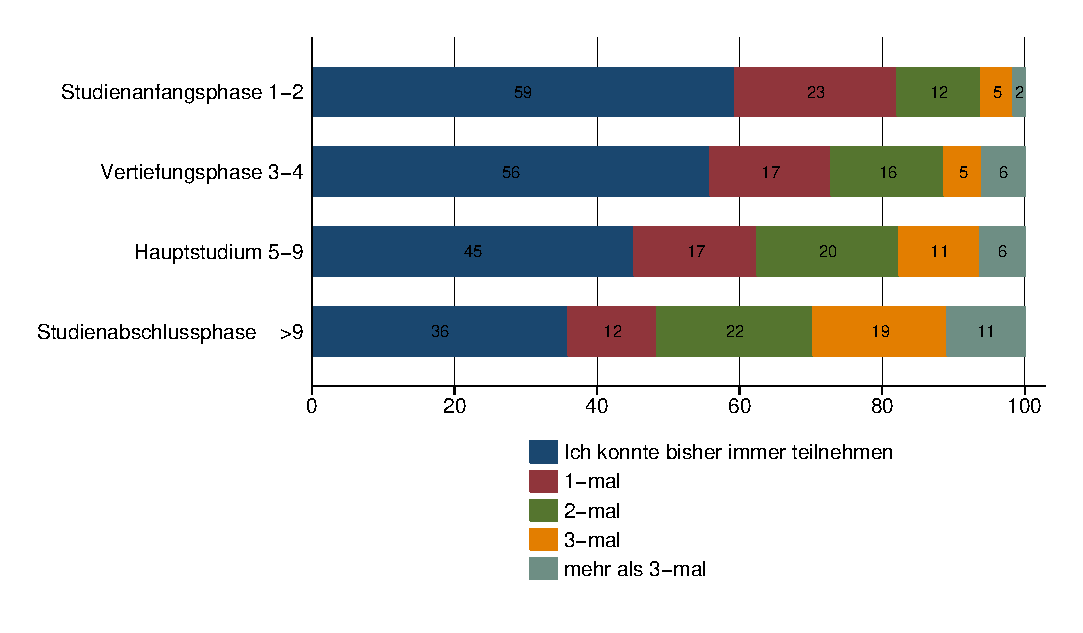
\includegraphics[
%  defaultresolution=72 !,
%  bmpsizefast=false
%]{image}
%\end{verbatim}
% \end{quote}
%
% \subsubsection{Hints}
%
% \begin{itemize}
% \item My version of \xfile{dvips.def} 1999/02/16 v3.0i defines
%       rules for the supported bitmap extensions, but does not
%       include them in the list of extensions that are tried
%       if the file name is not given with an extension.
%       In such a case, the list of extensions can be set
%       by \cs{DeclareGraphicsExtensions}, see \xpackage{grfguide}.
%       The following code just extends the list:
%       \begin{quote}
%\begin{verbatim}
%\makeatletter
%\g@addto@macro\Gin@extensions{,.bmp,.pcx,.msp}
%\makeatother
%\end{verbatim}
%       \end{quote}
% \item My version of \xfile{dvipdfm.def} 1998/11/24 vx.x misses
%       the graphics rule for PNG files. It can be added by:
%       \begin{quote}
%\begin{verbatim}
%\DeclareGraphicsRule{.png}{bmp}{.bb}{#1}
%\end{verbatim}
%       \end{quote}
%       See the previous issue to add the extension \xfile{.png} to the list
%       of extensions for package \xpackage{graphics}.
% \end{itemize}
%
% \subsubsection{Test program}
%
% There is a test program \xfile{bmpsize-test.tex}. Run it through
% \verb|latex|, \verb|pdflatex|, or \verb|pdftex|. Then given
% image files are inspected and the result is printed.
%
% \subsubsection{Interface for programmers}
%
% The macro names of the parsers are \verb|\bmpsize@read@|\meta{type}.
% Example: \cs{bmpsize@read@jpg} in case of JPEG.
%
% A parser sets the switch \cs{ifbmpsize@ok} to true, if it
% could successfully parse the image file.
% The width and height are returnd in \cs{bmpsize@width} and
% \cs{bmpsize@height}. If information about density is available,
% it is used to calculate width and height of the image, otherwise
% the values given by option \xoption{defaultresolution} is used.
% \xoption{resolution} overwrites the values in the image file.
%
% \subsection{Improved bitmap inclusion}
%
% Some drivers for package \xpackage{graphics} define the graphics
% type \xoption{bmp} for bitmap images. The code in the standard
% drivers for \xoption{dvips}, \xoption{dvipdfm}, and \xoption{dvipdfmx}
% is very basic and misses essential features of the
% package \xpackage{graphicx}. Therefore the code for bitmap
% inclusion is automatically rewritten by this package to add
% the following features:
% \begin{itemize}
% \item Support for \xoption{viewport} and \xoption{trim}.
% \item Support for \xoption{clip}.
% \item In case of \xoption{dvipdfm} and \xoption{dvipdfmx} the
%       bitmap images are reused and not included again if they
%       are used more than once.
% \end{itemize}
% However, there is a difference between \xoption{dvipdfm} and
% \xoption{dvipdfmx}, especially if images are reused. In the
% former case the reused box has width and height of 1bp, in the
% latter case its natural width. Thus the correct driver option must be given.
% \xoption{dvipdfm} and \xoption{dvipdfmx} are not equivalent.
%
% Older versions of \xoption{dvipdfmx} uses a size of 1in. However I do
% want to distinguish between versions of the same program. Therefore the
% support of these older versions has stopped with version 1.6 of this package.
% Use version dvipdfmx-20090708 or newer (some few versions before will
% probably also work, but I don't want to investigate this further).
%
% \StopEventually{
% }
%
% \section{Implementation}
%
% \subsection{Basic package \xpackage{bmpsize-base}}
%
%    Identification.
%    \begin{macrocode}
%<*base>
\ProvidesPackage{bmpsize-base}%
  [2009/09/04 v1.6 Basic part of bmpsize (HO)]%
%    \end{macrocode}
%    Modules of package \xpackage{fp} are used for calculations.
%    \begin{macrocode}
\RequirePackage{fp-basic}
\RequirePackage{fp-snap}
%    \end{macrocode}
%    Package \xpackage{fp} uses nested \cs{loop} structures.
%    That breaks with the plain-\TeX\ version of \cs{loop}.
%    Therefore we use the \LaTeX\ variant.
%    \begin{macro}{\@bmpsize@plain@loop}
%    \begin{macrocode}
\long\def\@bmpsize@plain@loop#1\repeat{%
  \def\iterate{%
    #1\relax
    \expandafter\iterate\fi
  }%
  \iterate
  \let\iterate\relax
}
%    \end{macrocode}
%    \end{macro}
%    \begin{macrocode}
\RequirePackage{pdftexcmds}[2007/11/11]
%    \end{macrocode}
%    \begin{macrocode}
\newif\ifbmpsize@ok
\let\@bmpsize@ok\bmpsize@oktrue

\newif\if@bmpsize@bigendian
\newif\if@bmpsize@absnum
\newif\if@bmpsize@user@resolution
\newif\if@bmpsize@fast
\@bmpsize@fasttrue

\def\@bmpsize@init{%
  \let\@bmpsize@org@plain@loop\loop
  \let\loop\@bmpsize@plain@loop
  \bmpsize@okfalse
  \@bmpsize@bigendiantrue
  \@bmpsize@absnumfalse
  \let\bmpsize@pixelwidth\relax
  \let\bmpsize@pixelheight\relax
  \let\bmpsize@pixelx\relax
  \let\bmpsize@pixely\relax
  \let\bmpsize@unit\relax
  \let\bmpsize@pixelxdenom\relax
  \let\bmpsize@pixelydenom\relax
  \let\bmpsize@orientation\relax
}

\def\@bmpsize@stop#1\@nil{}

\def\@bmpsize@loop#1{%
  #1%
  \@bmpsize@loop{#1}%
}
\def\@bmpsize@break#1\@bmpsize@loop#2{}

\def\@bmpsize@size#1#2#3{%
  \edef#3{\pdf@filesize{#1}}%
  \ifx#3\@empty
    \expandafter\@bmpsize@stop
  \fi
  \ifnum#3<#2\relax
    \expandafter\@bmpsize@stop
  \fi
}

\def\@bmpsize@read#1#2#3{%
  \edef\@bmpsize@buf{\pdf@filedump{#3}{#2}{#1}}%
  \edef\@bmpsize@temp{%
    \noexpand\@bmpsize@check@byte{#2}\@bmpsize@buf{}{}\noexpand\\%
  }%
  \@bmpsize@temp
}
\def\@bmpsize@fillbuf#1{%
  \ifx\@bmpsize@buf\@empty
    \expandafter\@firstofone
  \else
    \expandafter\@gobble
  \fi
  {%
    \edef\@bmpsize@buf{%
      \pdf@filedump{\bmpsize@offset}{\bmpsize@fillbuflength}{#1}%
    }%
    \ifx\@bmpsize@buf\@empty
      \expandafter\@bmpsize@stop
    \fi
    \edef\bmpsize@offset{\the\numexpr\bmpsize@offset+\bmpsize@fillbuflength}%
  }%
}
\def\bmpsize@fillbuflength{10}

\def\@bmpsize@append#1#2#3{%
  \edef#1{#2#3}%
}
\def\@bmpsize@pushback#1{%
  \edef\@bmpsize@buf{#1\@bmpsize@buf}%
}

\def\@bmpsize@iswhite#1{%
  \ifnum\pdf@strcmp{#1}{09}=\z@
  \else
    \ifnum\pdf@strcmp{#1}{0A}=\z@
    \else
      \ifnum\pdf@strcmp{#1}{0D}=\z@
      \else
        \ifnum\pdf@strcmp{#1}{20}=\z@
        \else
          1%
        \fi
      \fi
    \fi
  \fi
  \space
}
\def\@bmpsize@isdigit#1{%
  \ifnum\pdf@strcmp{#1}{30}<\z@
    1%
  \else
    \ifnum\pdf@strcmp{#1}{39}>\z@
      1%
    \fi
  \fi
  \space
}

\def\@bmpsize@check@byte#1#2#3{%
  \ifnum#1<\@ne
    \csname fi\endcsname
    \@bmpsize@cleanup@end
  \else
    \csname fi\endcsname
  \ifx!#2#3!%
    \csname fi\endcsname
    \@bmpsize@stop
  \else
    \csname fi\endcsname
    \expandafter\@bmpsize@check@byte\expandafter{\the\numexpr#1-1}%
}
\def\@bmpsize@cleanup@end#1\\{}

\def\@bmpsize@swap@maybe#1{%
  \if@bmpsize@bigendian
  \else
    \edef#1{\expandafter\@bmpsize@@swap#1\@empty\@empty\@empty\@empty}%
  \fi
}
\def\@bmpsize@@swap#1#2#3#4#5#6#7#8{%
  #7#8#5#6#3#4#1#2%
}

\def\@bmpsize@skip@one{%
  \edef\@bmpsize@buf{\expandafter\@gobbletwo\@bmpsize@buf}%
}
\def\@bmpsize@skip@two{%
  \edef\@bmpsize@buf{\expandafter\@gobblefour\@bmpsize@buf}%
}
\def\@bmpsize@skip@four{%
  \edef\@bmpsize@buf{%
    \expandafter\expandafter\expandafter\@gobblefour\expandafter
    \@gobblefour\@bmpsize@buf
  }%
}

\def\@bmpsize@grab#1#2{%
  \edef#1{\noexpand\@bmpsize@grab@byte#2=\@bmpsize@buf\noexpand\\}%
  \edef#1{#1}%
}
\def\@bmpsize@grab@byte#1=#2#3{%
  #2#3%
  \ifnum#1>\@ne
    \expandafter\@bmpsize@grab@byte\the\numexpr#1-1\expandafter=%
  \else
    \expandafter\@bmpsize@cleanup@end
  \fi
}

\def\@bmpsize@abs@maybe#1{%
  \let\@bmpsize@temp\relax
  \if@bmpsize@absnum
    \ifnum"\expandafter\@car#1\@nil>7 %
      \edef#1{\expandafter\@bmpsize@abs@byte#1\relax}%
      \ifnum\pdf@strcmp{#1}{7FFFFFFF}=\z@
        \let\@bmpsize@temp\@bmpsize@stop
      \else
        \def\@bmpsize@temp{\edef#1{\the\numexpr#1+1}}%
      \fi
    \fi
  \fi
}
\def\@bmpsize@abs@byte#1{%
  \ifx#1\relax
  \else
    \ifcase"0#1 %
      F\or E\or D\or C\or B\or A\or 9\or 8\or
      7\or 6\or 5\or 4\or 3\or 2\or 1\or 0%
    \fi
    \expandafter\@bmpsize@abs@byte
  \fi
}

\def\@bmpsize@num@one#1{%
  \@bmpsize@grab#11%
  \@bmpsize@abs@maybe#1%
  \edef#1{\number"#1}%
  \@bmpsize@temp
  \@bmpsize@skip@one
}
\def\@bmpsize@num@two#1{%
  \@bmpsize@grab#12%
  \@bmpsize@swap@maybe#1%
  \@bmpsize@abs@maybe#1%
  \edef#1{\number"#1}%
  \@bmpsize@temp
  \@bmpsize@skip@two
}
\def\@bmpsize@num@four#1{%
  \@bmpsize@grab#14%
  \@bmpsize@swap@maybe#1%
  \@bmpsize@abs@maybe#1%
  \ifnum\pdf@strcmp{#1}{7FFFFFFF}>\z@
    \expandafter\@bmpsize@stop
  \fi
  \edef#1{\number"#1}%
  \@bmpsize@temp
  \@bmpsize@skip@four
}

\def\@bmpsize@div#1#2#3{% #1 := #2/#3
  \FPdiv#1{#2}{#3}%
  \@bmpsize@beautify#1%
}
\def\@bmpsize@beautify#1{%
  \FPifint#1%
    \edef#1{\expandafter\@bmpsize@trunc#1.\@nil}%
  \else
    \edef#1{\expandafter\@bmpsize@cleanup@frac#1.\@nil}%
  \fi
}
\def\@bmpsize@trunc#1.#2\@nil{#1}
% #1 isn't an integer, thus we should have at least one
% necessary digit after the dot
\def\@bmpsize@cleanup@frac#1.#2#3.#4\@nil{%
  #1.#2%
  \ifx\\#3\\%
  \else
    \@bmpsize@cleanup@fracdigits#3000000000\@nil
  \fi
}
\def\@bmpsize@cleanup@fracdigits#1#2#3#4#5#6#7#8#9{%
  \ifcase#9 %
    \ifcase#8 %
      \ifcase#7 %
        \ifcase#6 %
          \ifcase#5 %
            \ifcase #4 %
              \ifcase #3 %
                \ifcase #2 %
                  \ifcase #1 %
                  \else
                    #1%
                  \fi
                \else
                  #1#2%
                \fi
              \else
                #1#2#3%
              \fi
            \else
              #1#2#3#4%
            \fi
          \else
            #1#2#3#4#5%
          \fi
        \else
          #1#2#3#4#5#6%
        \fi
      \else
        #1#2#3#4#5#6#7%
      \fi
    \else
      #1#2#3#4#5#6#7#8%
    \fi
  \else
    #1#2#3#4#5#6#7#8#9%
  \fi
  \@bmpsize@trunc.%
}

\def\@bmpsize@end{%
  \ifbmpsize@ok
    \ifx\bmpsize@pixelwidth\relax
      \bmpsize@okfalse
    \fi
    \ifx\bmpsize@pixelheight\relax
      \bmpsize@okfalse
    \fi
  \fi
  \ifbmpsize@ok
    \ifnum\bmpsize@pixelwidth>\z@
    \else
      \bmpsize@okfalse
    \fi
    \ifnum\bmpsize@pixelheight>\z@
    \else
      \bmpsize@okfalse
    \fi
  \fi
  \ifbmpsize@ok
    \ifcase 0%
      \ifx\bmpsize@pixelx\relax 1 \fi
      \ifx\bmpsize@pixely\relax 1 \fi
      \ifnum\bmpsize@pixelx>\z@\else 1 \fi
      \ifnum\bmpsize@pixely>\z@\else 1 \fi
      \ifx\bmpsize@pixelxdenom\relax
         \ifx\bmpsize@pixelydenom\relax\else 1 \fi
      \else
        \ifnum\bmpsize@pixelxdenom>\z@\else 1 \fi
      \fi
      \ifx\bmpsize@pixelydenom\relax
      \else
        \ifnum\bmpsize@pixelydenom>\z@\else 1 \fi
      \fi
    \else
      \let\bmpsize@pixelx\relax
      \let\bmpsize@pixely\relax
      \let\bmpsize@unit\relax
      \let\bmpsize@pixelxdenom\relax
      \let\bmpsize@pixelydenom\relax
    \fi
    \ifx\bmpsize@pixelxdenom\relax
    \else
      \@bmpsize@div\bmpsize@pixelx\bmpsize@pixelx\bmpsize@pixelxdenom
      \@bmpsize@div\bmpsize@pixely\bmpsize@pixely\bmpsize@pixelydenom
      \let\bmpsize@pixelxdenom\relax
      \let\bmpsize@pixelydenom\relax
    \fi
    \ifcase 0\ifx\bmpsize@unit\relax 1\fi
             \if@bmpsize@user@resolution 1\fi
             \relax
      \let\bmpsize@calc@unit\bmpsize@unit
      \let\bmpsize@calc@pixelx\bmpsize@pixelx
      \let\bmpsize@calc@pixely\bmpsize@pixely
    \else
      \let\bmpsize@calc@unit\bmpsize@unit@default
      \let\bmpsize@calc@pixelx\bmpsize@pixelx@default
      \let\bmpsize@calc@pixely\bmpsize@pixely@default
      \ifx\bmpsize@calc@pixely\Gin@exclamation
        \ifx\bmpsize@pixelx\relax
          \let\bmpsize@calc@pixely\bmpsize@calc@pixelx
        \else
          \FPdiv\bmpsize@calc@pixely\bmpsize@calc@pixelx\bmpsize@pixelx
          \FPmul\bmpsize@calc@pixely\bmpsize@calc@pixely\bmpsize@pixely
        \fi
      \else
        \ifx\bmpsize@calc@pixelx\Gin@exclamation
          \ifx\bmpsize@pixelx\relax
            \let\bmpsize@calc@pixelx\bmpsize@calc@pixely
          \else
            \FPdiv\bmpsize@calc@pixelx\bmpsize@calc@pixely\bmpsize@pixely
            \FPmul\bmpsize@calc@pixelx\bmpsize@calc@pixelx\bmpsize@pixelx
          \fi
        \fi
      \fi
    \fi
    \FPdiv\bmpsize@width\bmpsize@pixelwidth\bmpsize@calc@pixelx
    \FPdiv\bmpsize@height\bmpsize@pixelheight\bmpsize@calc@pixely
    % calculation of width and height in bp for package graphics
    % 1in = 72bp = 72.27pt, 72/72.27 = 8/8.03, 1pt = 65536sp
    \if@bmpsize@fast
      \edef\bmpsize@width{%
        \strip@pt\dimexpr.99626\dimexpr
        \bmpsize@width\dimexpr\bmpsize@calc@unit
      }%
      \edef\bmpsize@height{%
        \strip@pt\dimexpr.99626\dimexpr
        \bmpsize@height\dimexpr\bmpsize@calc@unit
      }%
    \else
      \edef\@bmpsize@temp{\number\dimexpr\bmpsize@calc@unit}%
      \ifnum\@bmpsize@temp>100000 %
        \FPmul\@bmpsize@temp\@bmpsize@temp{0.00001}%
        \def\@bmpsize@corr{100000}%
      \else
        \let\@bmpsize@corr\relax
      \fi
      \FPmul\bmpsize@width\bmpsize@width\@bmpsize@temp
      \FPmul\bmpsize@height\bmpsize@height\@bmpsize@temp
      \FPmul\bmpsize@width\bmpsize@width{8}%
      \FPmul\bmpsize@height\bmpsize@height{8}%
      \FPdiv\bmpsize@width\bmpsize@width{8.03}%
      \FPdiv\bmpsize@height\bmpsize@height{8.03}%
      \FPdiv\bmpsize@width\bmpsize@width{65536}%
      \FPdiv\bmpsize@height\bmpsize@height{65536}%
      \ifx\@bmpsize@corr\relax
      \else
        \FPmul\bmpsize@width\bmpsize@width\@bmpsize@corr
        \FPmul\bmpsize@height\bmpsize@height\@bmpsize@corr
      \fi
      \FPround\bmpsize@width\bmpsize@width{5}%
      \FPround\bmpsize@height\bmpsize@height{5}%
      \@bmpsize@beautify\bmpsize@width
      \@bmpsize@beautify\bmpsize@height
    \fi
  \fi
  \let\loop\@bmpsize@org@plain@loop
}
\def\bmpsize@unit@default{72.27pt}% more accurate than 1in
\def\bmpsize@pixelx@default{72}
\let\bmpsize@pixely@default\Gin@exclamation

\def\bmpsize@types{png,jpg,bmp,gif,tiff,pnm,pam,xpm,tga,pcx,msp,sgi}
%</base>
%    \end{macrocode}
%
% \subsection{Bitmap formats}
%
% \subsubsection{png}
%
%\iffalse
%<*ignore>
%\fi
%\begin{verbatim}
%begin png
%big-endian
%
%read 24 0
%grab 8        -> $temp
%check streq $temp [0x89 "PNG" 0x0D 0x0A 0x1A 0x0A]
%num 4         -> $length
%grab 4        -> $temp
%check streq $temp ["IHDR"]
%num 4         -> $pixelwidth
%num 4         -> $pixelheight
%ok
%assign numexpr(20 + $length) -> $offset
%loop
%  read 8 $offset
%  num 4       -> $length
%  grab 4      -> $temp
%  if streq $temp ["IDAT"]
%    stop
%  fi
%  if streq $temp ["pHYs"]
%    read 9 numexpr($offset + 8)
%    num 4     -> $pixelx
%    num 4     -> $pixely
%    grab 1     -> $temp
%    if numeq $temp 1
%      assign {100cm} -> $unit
%    fi
%    stop
%  fi
%  assign numexpr($offset + 12 + $length) -> $offset
%repeat
%end
%\end{verbatim}
%\iffalse
%</ignore>
%\fi
%    \begin{macro}{\bmpsize@read@png}
%    \begin{macrocode}
%<*base>
\def\bmpsize@read@png#1{%
  \@bmpsize@init
  \@bmpsize@bigendiantrue
  \@bmpsize@read{#1}{24}{0}%
  \@bmpsize@grab\bmpsize@temp{8}%
  \@bmpsize@skip@four
  \@bmpsize@skip@four
  \ifnum\pdf@strcmp{\bmpsize@temp}{89504E470D0A1A0A}=\z@
  \else
    \expandafter\@bmpsize@stop
  \fi
  \@bmpsize@num@four\bmpsize@length
  \@bmpsize@grab\bmpsize@temp{4}%
  \@bmpsize@skip@four
  \ifnum\pdf@strcmp{\bmpsize@temp}{49484452}=\z@
  \else
    \expandafter\@bmpsize@stop
  \fi
  \@bmpsize@num@four\bmpsize@pixelwidth
  \@bmpsize@num@four\bmpsize@pixelheight
  \@bmpsize@ok
  \edef\bmpsize@offset{\the\numexpr20+\bmpsize@length}%
  \@bmpsize@loop{%
    \@bmpsize@read{#1}{8}{\bmpsize@offset}%
    \@bmpsize@num@four\bmpsize@length
    \@bmpsize@grab\bmpsize@temp{4}%
    \@bmpsize@skip@four
    \ifnum\pdf@strcmp{\bmpsize@temp}{49444154}=\z@
      \expandafter\@firstofone
    \else
      \expandafter\@gobble
    \fi
    {%
      \@bmpsize@stop
    }%
    \ifnum\pdf@strcmp{\bmpsize@temp}{70485973}=\z@
      \expandafter\@firstofone
    \else
      \expandafter\@gobble
    \fi
    {%
      \@bmpsize@read{#1}{9}{\numexpr\bmpsize@offset+8\relax}%
      \@bmpsize@num@four\bmpsize@pixelx
      \@bmpsize@num@four\bmpsize@pixely
      \@bmpsize@grab\bmpsize@temp{1}%
      \@bmpsize@skip@one
      \ifnum\bmpsize@temp=1\relax
        \expandafter\@firstofone
      \else
        \expandafter\@gobble
      \fi
      {%
        \def\bmpsize@unit{100cm}%
      }%
      \@bmpsize@stop
    }%
    \edef\bmpsize@offset{\the\numexpr\bmpsize@offset+12+\bmpsize@length}%
  }%
  \@bmpsize@stop
  \@nil
  \@bmpsize@end
}%
%</base>
%    \end{macrocode}
%    \end{macro}
%
% \subsubsection{jpg}
%
%\iffalse
%<*ignore>
%\fi
%\begin{verbatim}
%begin jpg
%
%read 3 0
%grab 3      -> $temp % SOI and 0xFF
%check streq $temp [0xFF 0xD8 0xFF]
%assign {2} -> $offset
%assign {0} -> $exifdensity
%loop
%  read 4 $offset
%  grab 1    -> $temp
%  check streq $temp [0xFF]
%  num 1    -> $temp
%  if numeq $temp 0xDA % SOS
%    stop
%  fi
%  % look for JFIF APP0 segment
%  if numeq $temp 0xE0 % APP0
%    num 2       -> $length
%    if numeq $exifdensity 0
%      if numge $length 16 % a JFIF segment has 16 bytes at least
%        read 12 numexpr($offset + 4)
%        grab 5      -> $temp % identifier
%        if streq $temp ["JFIF" 0x0]
%          check numge $length 16
%          skip 2 % version
%          num 1       -> $temp % units
%          if numeq $temp 1
%            assign {72.27pt} -> $unit
%          else
%            if numeq $temp 2
%              assign {1cm} -> $unit
%            fi
%          fi
%          num 2    -> $pixelx
%          num 2    -> $pixely
%        fi
%      fi
%    fi
%  else
%    if numeq $temp 0xE1 % APP1
%      % look for Exif APP1 segment
%      num 2 -> $length
%      if numge $length 20 % identifier (6) + Tiff header (8) + first IFD (>=6)
%        read 20 numexpr($offset + 4)
%        grab 6 -> $temp
%        if streq $temp ["Exif" 0x0 0x0]
%          assign numexpr($offset + 10) -> $exifoffset
%          % read TIFF header
%          grab 2 -> $temp
%          if streq $temp ["II"]
%            little-endian
%          else
%            check streq $temp ["MM"]
%            % big-endian
%          fi
%          num 2 -> $temp
%          check numeq $temp 42
%          num 4 -> $temp % offset of first IFD
%          check numgt $temp 0
%          % read first IFD
%          assign numexpr($temp + $exifoffset) -> $off
%          read 2 $off
%          num 2 -> $entries
%          assign numexpr($off + 2) -> $off
%          loop
%            if numeq $entries 0
%              break
%            fi
%            assign numexpr($entries - 1) -> $entries
%            % entry format:
%            % 2 tag
%            % 2 field type
%            % 4 count
%            % 4 value/offset
%            read 12 $off
%            assign numexpr($off + 12) -> $off
%            num 2 -> $tag
%            if numeq $tag 296 % ResolutionUnit
%              skip 6 % type: 3 (short), count: 1
%              num 2 -> $temp
%              ifcase $temp
%              or % 1
%                clear $unit
%              or % 2
%                assign {72.27pt} -> $unit
%              or % 3
%                assign {1cm} -> $unit
%              else
%                clear $unit % unknown
%              fi
%              ifcase $temp
%              or % 1
%              or % 2
%                assign {1} -> $exifdensity
%              or % 3
%                assign {1} -> $exifdensity
%              else
%                assign $exifdensity -> $exifdensity
%              fi
%            fi
%            % 256 ImageWidth (use width of JPG part)
%            % 257 ImageHeight (use height of JPG part)
%            if numeq $tag 274 % Orientation
%              skip 6 % type: 3 (short), count: 1
%              num 2 -> $temp
%              if numge $temp 0 
%                if numle $temp 8
%                  assign $temp -> $orientation
%                fi
%              fi
%            fi
%            if numeq $tag 282 % XResolution
%              skip 6
%              num 4 -> $temp
%              read 8 numexpr($temp + $exifoffset)
%              num 4 -> $pixelx
%              num 4 -> $temp
%              if numeq $temp 1
%              else
%                assign numexpr($temp) -> $pixelxdenom
%                % div $pixelx $temp -> $pixelx
%              fi
%            fi
%            if numeq $tag 283 % YResolution
%              skip 6
%              num 4 -> $temp
%              read 8 numexpr($temp + $exifoffset)
%              num 4 -> $pixely
%              num 4 -> $temp
%              if numeq $temp 1
%              else
%                assign numexpr($temp) -> $pixelydenom
%                % div $pixely $temp -> $pixely
%              fi
%            fi
%          repeat
%          big-endian
%        fi
%      fi
%    else
%      assign numexpr($temp - 0xC0) -> $temp
%      ifcase $temp % SOF_0
%      or % SOF_1
%      or % SOF_2
%      or % SOF_3
%      or % DHT
%        assign {-1} -> $temp
%      or % SOF_5
%      or % SOF_6
%      or % SOF_7
%      or % JPG
%        assign {-1} -> $temp
%      or % SOF_9
%      or % SOF_10
%      or % SOF_11
%      or % DAC
%        assign {-1} -> $temp
%      or % SOF_13
%      or % SOF_14
%      or % SOF_15
%      else
%        assign {-1} -> $temp
%      fi
%      if numeq $temp -1
%      else
%        read 4 numexpr($offset + 5)
%        num 2  -> $pixelheight
%        num 2  -> $pixelwidth
%        if numeq $pixelheight 0
%          clear $pixelheight
%          stop
%        fi
%        ok
%        stop
%      fi
%      num 2 -> $length
%    fi
%  fi
%  assign numexpr($offset + $length + 2) -> $offset
%repeat
%end
%\end{verbatim}
%\iffalse
%</ignore>
%\fi
%    \begin{macro}{\bmpsize@read@jpg}
%    \begin{macrocode}
%<*base>
\def\bmpsize@read@jpg#1{%
  \@bmpsize@init
  \@bmpsize@read{#1}{3}{0}%
  \@bmpsize@grab\bmpsize@temp{3}%
  \@bmpsize@skip@two
  \@bmpsize@skip@one
  \ifnum\pdf@strcmp{\bmpsize@temp}{FFD8FF}=\z@
  \else
    \expandafter\@bmpsize@stop
  \fi
  \def\bmpsize@offset{2}%
  \def\bmpsize@exifdensity{0}%
  \@bmpsize@loop{%
    \@bmpsize@read{#1}{4}{\bmpsize@offset}%
    \@bmpsize@grab\bmpsize@temp{1}%
    \@bmpsize@skip@one
    \ifnum\pdf@strcmp{\bmpsize@temp}{FF}=\z@
    \else
      \expandafter\@bmpsize@stop
    \fi
    \@bmpsize@num@one\bmpsize@temp
    \ifnum\bmpsize@temp=218\relax
      \expandafter\@firstofone
    \else
      \expandafter\@gobble
    \fi
    {%
      \@bmpsize@stop
    }%
    \ifnum\bmpsize@temp=224\relax
      \expandafter\@firstoftwo
    \else
      \expandafter\@secondoftwo
    \fi
    {%
      \@bmpsize@num@two\bmpsize@length
      \ifnum\bmpsize@exifdensity=0\relax
        \expandafter\@firstofone
      \else
        \expandafter\@gobble
      \fi
      {%
        \unless\ifnum\bmpsize@length<16\relax
          \expandafter\@firstofone
        \else
          \expandafter\@gobble
        \fi
        {%
          \@bmpsize@read{#1}{12}{\numexpr\bmpsize@offset+4\relax}%
          \@bmpsize@grab\bmpsize@temp{5}%
          \@bmpsize@skip@four
          \@bmpsize@skip@one
          \ifnum\pdf@strcmp{\bmpsize@temp}{4A46494600}=\z@
            \expandafter\@firstofone
          \else
            \expandafter\@gobble
          \fi
          {%
            \ifnum\bmpsize@length<16\relax
              \expandafter\@bmpsize@stop
            \fi
            \@bmpsize@skip@two
            \@bmpsize@num@one\bmpsize@temp
            \ifnum\bmpsize@temp=1\relax
              \expandafter\@firstoftwo
            \else
              \expandafter\@secondoftwo
            \fi
            {%
              \def\bmpsize@unit{72.27pt}%
            }{%
              \ifnum\bmpsize@temp=2\relax
                \expandafter\@firstofone
              \else
                \expandafter\@gobble
              \fi
              {%
                \def\bmpsize@unit{1cm}%
              }%
            }%
            \@bmpsize@num@two\bmpsize@pixelx
            \@bmpsize@num@two\bmpsize@pixely
          }%
        }%
      }%
    }{%
      \ifnum\bmpsize@temp=225\relax
        \expandafter\@firstoftwo
      \else
        \expandafter\@secondoftwo
      \fi
      {%
        \@bmpsize@num@two\bmpsize@length
        \unless\ifnum\bmpsize@length<20\relax
          \expandafter\@firstofone
        \else
          \expandafter\@gobble
        \fi
        {%
          \@bmpsize@read{#1}{20}{\numexpr\bmpsize@offset+4\relax}%
          \@bmpsize@grab\bmpsize@temp{6}%
          \@bmpsize@skip@four
          \@bmpsize@skip@two
          \ifnum\pdf@strcmp{\bmpsize@temp}{457869660000}=\z@
            \expandafter\@firstofone
          \else
            \expandafter\@gobble
          \fi
          {%
            \edef\bmpsize@exifoffset{\the\numexpr\bmpsize@offset+10}%
            \@bmpsize@grab\bmpsize@temp{2}%
            \@bmpsize@skip@two
            \ifnum\pdf@strcmp{\bmpsize@temp}{4949}=\z@
              \expandafter\@firstoftwo
            \else
              \expandafter\@secondoftwo
            \fi
            {%
              \@bmpsize@bigendianfalse
            }{%
              \ifnum\pdf@strcmp{\bmpsize@temp}{4D4D}=\z@
              \else
                \expandafter\@bmpsize@stop
              \fi
            }%
            \@bmpsize@num@two\bmpsize@temp
            \ifnum\bmpsize@temp=42\relax
            \else
              \expandafter\@bmpsize@stop
            \fi
            \@bmpsize@num@four\bmpsize@temp
            \ifnum\bmpsize@temp>0\relax
            \else
              \expandafter\@bmpsize@stop
            \fi
            \edef\bmpsize@off{\the\numexpr\bmpsize@temp+\bmpsize@exifoffset}%
            \@bmpsize@read{#1}{2}{\bmpsize@off}%
            \@bmpsize@num@two\bmpsize@entries
            \edef\bmpsize@off{\the\numexpr\bmpsize@off+2}%
            \@bmpsize@loop{%
              \ifnum\bmpsize@entries=0\relax
                \expandafter\@firstofone
              \else
                \expandafter\@gobble
              \fi
              {%
                \@bmpsize@break
              }%
              \edef\bmpsize@entries{\the\numexpr\bmpsize@entries-1}%
              \@bmpsize@read{#1}{12}{\bmpsize@off}%
              \edef\bmpsize@off{\the\numexpr\bmpsize@off+12}%
              \@bmpsize@num@two\bmpsize@tag
              \ifnum\bmpsize@tag=296\relax
                \expandafter\@firstofone
              \else
                \expandafter\@gobble
              \fi
              {%
                \@bmpsize@skip@four
                \@bmpsize@skip@two
                \@bmpsize@num@two\bmpsize@temp
                \ifcase\bmpsize@temp\relax
                \or
                  \let\bmpsize@unit\relax
                \or
                  \def\bmpsize@unit{72.27pt}%
                \or
                  \def\bmpsize@unit{1cm}%
                \else
                  \let\bmpsize@unit\relax
                \fi
                \ifcase\bmpsize@temp\relax
                \or
                \or
                  \def\bmpsize@exifdensity{1}%
                \or
                  \def\bmpsize@exifdensity{1}%
                \else
                  \let\bmpsize@exifdensity\bmpsize@exifdensity
                \fi
              }%
              \ifnum\bmpsize@tag=274\relax
                \expandafter\@firstofone
              \else
                \expandafter\@gobble
              \fi
              {%
                \@bmpsize@skip@four
                \@bmpsize@skip@two
                \@bmpsize@num@two\bmpsize@temp
                \unless\ifnum\bmpsize@temp<0\relax
                  \expandafter\@firstofone
                \else
                  \expandafter\@gobble
                \fi
                {%
                  \unless\ifnum\bmpsize@temp>8\relax
                    \expandafter\@firstofone
                  \else
                    \expandafter\@gobble
                  \fi
                  {%
                    \let\bmpsize@orientation\bmpsize@temp
                  }%
                }%
              }%
              \ifnum\bmpsize@tag=282\relax
                \expandafter\@firstofone
              \else
                \expandafter\@gobble
              \fi
              {%
                \@bmpsize@skip@four
                \@bmpsize@skip@two
                \@bmpsize@num@four\bmpsize@temp
                \@bmpsize@read{#1}{8}{\numexpr\bmpsize@temp+\bmpsize@exifoffset\relax}%
                \@bmpsize@num@four\bmpsize@pixelx
                \@bmpsize@num@four\bmpsize@temp
                \ifnum\bmpsize@temp=1\relax
                  \expandafter\@gobble
                \else
                  \expandafter\@firstofone
                \fi
                {%
                  \edef\bmpsize@pixelxdenom{\the\numexpr\bmpsize@temp}%
                }%
              }%
              \ifnum\bmpsize@tag=283\relax
                \expandafter\@firstofone
              \else
                \expandafter\@gobble
              \fi
              {%
                \@bmpsize@skip@four
                \@bmpsize@skip@two
                \@bmpsize@num@four\bmpsize@temp
                \@bmpsize@read{#1}{8}{\numexpr\bmpsize@temp+\bmpsize@exifoffset\relax}%
                \@bmpsize@num@four\bmpsize@pixely
                \@bmpsize@num@four\bmpsize@temp
                \ifnum\bmpsize@temp=1\relax
                  \expandafter\@gobble
                \else
                  \expandafter\@firstofone
                \fi
                {%
                  \edef\bmpsize@pixelydenom{\the\numexpr\bmpsize@temp}%
                }%
              }%
            }%
            \@bmpsize@bigendiantrue
          }%
        }%
      }{%
        \edef\bmpsize@temp{\the\numexpr\bmpsize@temp-192}%
        \ifcase\bmpsize@temp\relax
        \or
        \or
        \or
        \or
          \def\bmpsize@temp{-1}%
        \or
        \or
        \or
        \or
          \def\bmpsize@temp{-1}%
        \or
        \or
        \or
        \or
          \def\bmpsize@temp{-1}%
        \or
        \or
        \or
        \else
          \def\bmpsize@temp{-1}%
        \fi
        \ifnum\bmpsize@temp=-1\relax
          \expandafter\@gobble
        \else
          \expandafter\@firstofone
        \fi
        {%
          \@bmpsize@read{#1}{4}{\numexpr\bmpsize@offset+5\relax}%
          \@bmpsize@num@two\bmpsize@pixelheight
          \@bmpsize@num@two\bmpsize@pixelwidth
          \ifnum\bmpsize@pixelheight=0\relax
            \expandafter\@firstofone
          \else
            \expandafter\@gobble
          \fi
          {%
            \let\bmpsize@pixelheight\relax
            \@bmpsize@stop
          }%
          \@bmpsize@ok
          \@bmpsize@stop
        }%
        \@bmpsize@num@two\bmpsize@length
      }%
    }%
    \edef\bmpsize@offset{\the\numexpr\bmpsize@offset+\bmpsize@length+2}%
  }%
  \@bmpsize@stop
  \@nil
  \@bmpsize@end
}%
%</base>
%    \end{macrocode}
%    \end{macro}
%
% \subsubsection{bmp}
%
%\iffalse
%<*ignore>
%\fi
%\begin{verbatim}
%begin bmp
%little-endian
%
%read 26 0
%grab 2 -> $temp
%check streq $temp ["BM"]
%skip 12
%% header size is 4 bytes in V3+, unknown for V1, V2,
%% known header sizes fit in 2 bytes
%num 2   -> $temp
%if numeq $temp 12 % V1
%  skip 2
%  num 2 -> $pixelwidth
%  num 2 -> $pixelheight
%  % no resolution entries
%  ok
%  stop
%fi
%if numeq $temp 64 % V2
%  skip 2
%  num 2 -> $pixelwidth
%  num 2 -> $pixelheight
%  % missing specification for resolution
%  ok
%  stop
%fi
%% V3, V4, V5
%skip 2
%num 4 -> $pixelwidth
%absnum 4 -> $pixelheight
%ok
%read 8 38
%num 4 -> $pixelx
%num 4 -> $pixely
%assign {100cm} -> $unit
%end
%\end{verbatim}
%\iffalse
%</ignore>
%\fi
%    \begin{macro}{\bmpsize@read@bmp}
%    \begin{macrocode}
%<*base>
\def\bmpsize@read@bmp#1{%
  \@bmpsize@init
  \@bmpsize@bigendianfalse
  \@bmpsize@read{#1}{26}{0}%
  \@bmpsize@grab\bmpsize@temp{2}%
  \@bmpsize@skip@two
  \ifnum\pdf@strcmp{\bmpsize@temp}{424D}=\z@
  \else
    \expandafter\@bmpsize@stop
  \fi
  \@bmpsize@skip@four
  \@bmpsize@skip@four
  \@bmpsize@skip@four
  \@bmpsize@num@two\bmpsize@temp
  \ifnum\bmpsize@temp=12\relax
    \expandafter\@firstofone
  \else
    \expandafter\@gobble
  \fi
  {%
    \@bmpsize@skip@two
    \@bmpsize@num@two\bmpsize@pixelwidth
    \@bmpsize@num@two\bmpsize@pixelheight
    \@bmpsize@ok
    \@bmpsize@stop
  }%
  \ifnum\bmpsize@temp=64\relax
    \expandafter\@firstofone
  \else
    \expandafter\@gobble
  \fi
  {%
    \@bmpsize@skip@two
    \@bmpsize@num@two\bmpsize@pixelwidth
    \@bmpsize@num@two\bmpsize@pixelheight
    \@bmpsize@ok
    \@bmpsize@stop
  }%
  \@bmpsize@skip@two
  \@bmpsize@num@four\bmpsize@pixelwidth
  \@bmpsize@absnumtrue
  \@bmpsize@num@four\bmpsize@pixelheight
  \@bmpsize@absnumfalse
  \@bmpsize@ok
  \@bmpsize@read{#1}{8}{38}%
  \@bmpsize@num@four\bmpsize@pixelx
  \@bmpsize@num@four\bmpsize@pixely
  \def\bmpsize@unit{100cm}%
  \@bmpsize@stop
  \@nil
  \@bmpsize@end
}%
%</base>
%    \end{macrocode}
%    \end{macro}
%
% \subsubsection{gif}
%
%\iffalse
%<*ignore>
%\fi
%\begin{verbatim}
%begin gif
%little-endian
%
%% Header
%read 13 0
%grab 3      -> $temp
%check streq $temp ["GIF"]
%skip 3      % version
%
%% Logical Screen Descriptor
%num 2       -> $pixelwidth
%num 2       -> $pixelheight
%skip 2
%num 1       -> $temp % Pixel Aspect Ratio
%if numeq $temp 0
%else
%  assign numexpr($temp + 15) -> $pixelx
%  assign {64}     -> $pixely
%fi
%ok
%end
%\end{verbatim}
%\iffalse
%</ignore>
%\fi
%    \begin{macro}{\bmpsize@read@gif}
%    \begin{macrocode}
%<*base>
\def\bmpsize@read@gif#1{%
  \@bmpsize@init
  \@bmpsize@bigendianfalse
  \@bmpsize@read{#1}{13}{0}%
  \@bmpsize@grab\bmpsize@temp{3}%
  \@bmpsize@skip@two
  \@bmpsize@skip@one
  \ifnum\pdf@strcmp{\bmpsize@temp}{474946}=\z@
  \else
    \expandafter\@bmpsize@stop
  \fi
  \@bmpsize@skip@two
  \@bmpsize@skip@one
  \@bmpsize@num@two\bmpsize@pixelwidth
  \@bmpsize@num@two\bmpsize@pixelheight
  \@bmpsize@skip@two
  \@bmpsize@num@one\bmpsize@temp
  \ifnum\bmpsize@temp=0\relax
    \expandafter\@gobble
  \else
    \expandafter\@firstofone
  \fi
  {%
    \edef\bmpsize@pixelx{\the\numexpr\bmpsize@temp+15}%
    \def\bmpsize@pixely{64}%
  }%
  \@bmpsize@ok
  \@bmpsize@stop
  \@nil
  \@bmpsize@end
}%
%</base>
%    \end{macrocode}
%    \end{macro}
%
% \subsubsection{tiff}
%
%\iffalse
%<*ignore>
%\fi
%\begin{verbatim}
%begin tiff
%% defaults
%assign {72.27pt} -> $unit
%
%% Image File Header
%read 8 0
%grab 2 -> $temp
%if streq $temp ["II"]
%  little-endian
%else
%  check streq $temp ["MM"]
%  big-endian
%fi
%num 2 -> $temp
%check numeq $temp 42
%num 4 -> $offset % first IFD (Image File Directory)
%
%% First IFD
%read 2 $offset
%assign numexpr($offset + 2) -> $offset
%num 2 -> $entries
%ok % must rely on checks at the end
%loop
%  if numeq $entries 0
%    stop
%  fi
%  assign numexpr($entries - 1) -> $entries
%  % entry format:
%  % 2 tag
%  % 2 field type
%  % 4 count
%  % 4 value/offset
%  read 12 $offset
%  assign numexpr($offset + 12) -> $offset
%  num 2 -> $tag % tag
%  if numeq $temp 296 % ResolutionUnit
%    skip 6 % type: 3 (short), count: 1
%    num 2 -> $temp
%    ifcase $temp
%    or % 1
%      clear $unit
%    or % 2
%      assign {72.27pt} -> $unit
%    or % 3
%      assign {1cm} -> $unit
%    else
%      clear $unit
%    fi
%  fi
%  if numeq $tag 256 % ImageWidth
%    skip 6
%    num 4 -> $pixelwidth
%  fi
%  if numeq $tag 257 % ImageLength
%    skip 6
%    num 4 -> $pixelheight
%  fi
%  if numeq $tag 282 % XResolution
%    skip 6
%    num 4 -> $temp
%    read 8 $temp
%    num 4 -> $pixelx
%    num 4 -> $temp
%    if numeq $temp 1
%    else
%      assign numexpr($temp) -> $pixelxdenom
%      % div $pixelx $temp -> $pixelx
%    fi
%  fi
%  if numeq $tag 283 % YResolution
%    skip 6
%    num 4 -> $temp
%    read 8 $temp
%    num 4 -> $pixely
%    num 4 -> $temp
%    if numeq $temp 1
%    else
%      assign numexpr($temp) -> $pixelydenom
%      % div $pixely $temp -> $pixely
%    fi
%  fi
%repeat
%end
%\end{verbatim}
%\iffalse
%</ignore>
%\fi
%    \begin{macro}{\bmpsize@read@tiff}
%    \begin{macrocode}
%<*base>
\def\bmpsize@read@tiff#1{%
  \@bmpsize@init
  \def\bmpsize@unit{72.27pt}%
  \@bmpsize@read{#1}{8}{0}%
  \@bmpsize@grab\bmpsize@temp{2}%
  \@bmpsize@skip@two
  \ifnum\pdf@strcmp{\bmpsize@temp}{4949}=\z@
    \expandafter\@firstoftwo
  \else
    \expandafter\@secondoftwo
  \fi
  {%
    \@bmpsize@bigendianfalse
  }{%
    \ifnum\pdf@strcmp{\bmpsize@temp}{4D4D}=\z@
    \else
      \expandafter\@bmpsize@stop
    \fi
    \@bmpsize@bigendiantrue
  }%
  \@bmpsize@num@two\bmpsize@temp
  \ifnum\bmpsize@temp=42\relax
  \else
    \expandafter\@bmpsize@stop
  \fi
  \@bmpsize@num@four\bmpsize@offset
  \@bmpsize@read{#1}{2}{\bmpsize@offset}%
  \edef\bmpsize@offset{\the\numexpr\bmpsize@offset+2}%
  \@bmpsize@num@two\bmpsize@entries
  \@bmpsize@ok
  \@bmpsize@loop{%
    \ifnum\bmpsize@entries=0\relax
      \expandafter\@firstofone
    \else
      \expandafter\@gobble
    \fi
    {%
      \@bmpsize@stop
    }%
    \edef\bmpsize@entries{\the\numexpr\bmpsize@entries-1}%
    \@bmpsize@read{#1}{12}{\bmpsize@offset}%
    \edef\bmpsize@offset{\the\numexpr\bmpsize@offset+12}%
    \@bmpsize@num@two\bmpsize@tag
    \ifnum\bmpsize@temp=296\relax
      \expandafter\@firstofone
    \else
      \expandafter\@gobble
    \fi
    {%
      \@bmpsize@skip@four
      \@bmpsize@skip@two
      \@bmpsize@num@two\bmpsize@temp
      \ifcase\bmpsize@temp\relax
      \or
        \let\bmpsize@unit\relax
      \or
        \def\bmpsize@unit{72.27pt}%
      \or
        \def\bmpsize@unit{1cm}%
      \else
        \let\bmpsize@unit\relax
      \fi
    }%
    \ifnum\bmpsize@tag=256\relax
      \expandafter\@firstofone
    \else
      \expandafter\@gobble
    \fi
    {%
      \@bmpsize@skip@four
      \@bmpsize@skip@two
      \@bmpsize@num@four\bmpsize@pixelwidth
    }%
    \ifnum\bmpsize@tag=257\relax
      \expandafter\@firstofone
    \else
      \expandafter\@gobble
    \fi
    {%
      \@bmpsize@skip@four
      \@bmpsize@skip@two
      \@bmpsize@num@four\bmpsize@pixelheight
    }%
    \ifnum\bmpsize@tag=282\relax
      \expandafter\@firstofone
    \else
      \expandafter\@gobble
    \fi
    {%
      \@bmpsize@skip@four
      \@bmpsize@skip@two
      \@bmpsize@num@four\bmpsize@temp
      \@bmpsize@read{#1}{8}{\bmpsize@temp}%
      \@bmpsize@num@four\bmpsize@pixelx
      \@bmpsize@num@four\bmpsize@temp
      \ifnum\bmpsize@temp=1\relax
        \expandafter\@gobble
      \else
        \expandafter\@firstofone
      \fi
      {%
        \edef\bmpsize@pixelxdenom{\the\numexpr\bmpsize@temp}%
      }%
    }%
    \ifnum\bmpsize@tag=283\relax
      \expandafter\@firstofone
    \else
      \expandafter\@gobble
    \fi
    {%
      \@bmpsize@skip@four
      \@bmpsize@skip@two
      \@bmpsize@num@four\bmpsize@temp
      \@bmpsize@read{#1}{8}{\bmpsize@temp}%
      \@bmpsize@num@four\bmpsize@pixely
      \@bmpsize@num@four\bmpsize@temp
      \ifnum\bmpsize@temp=1\relax
        \expandafter\@gobble
      \else
        \expandafter\@firstofone
      \fi
      {%
        \edef\bmpsize@pixelydenom{\the\numexpr\bmpsize@temp}%
      }%
    }%
  }%
  \@bmpsize@stop
  \@nil
  \@bmpsize@end
}%
%</base>
%    \end{macrocode}
%    \end{macro}
%
% \subsubsection{pnm}
%
%\iffalse
%<*ignore>
%\fi
%\begin{verbatim}
%begin pnm
%assign {0} -> $offset
%read 3 $offset
%assign {3} -> $offset
%grab 1 -> $temp
%check streq $temp ["P"]
%grab 1 -> $temp
%check strge $temp ["1"]
%check strle $temp ["6"]
%% ensure one white space
%grab 1 -> $temp
%if iswhite $temp
%else
%  stop
%fi
%loop
%  % skip white space
%  fillbuf
%  grab 1 -> $temp
%  if iswhite $temp
%  else
%    if streq $temp ["#"]
%      % ignore comments
%      loop
%        fillbuf
%        grab 1 -> $temp
%        if streq $temp [0x0A]
%          break
%        else
%          if streq $temp [0x0D]
%            break
%          fi
%        fi
%      repeat
%    else
%      pushback $temp
%      break
%    fi
%  fi
%repeat
%assign {} -> $tempnum
%loop
%  fillbuf
%  grab 1 -> $temp
%  if isdigit $temp
%    append $tempnum $temp -> $tempnum
%  else
%    if iswhite $temp
%      break
%    else
%      stop
%    fi
%  fi
%repeat
%assign unescapehex($tempnum) -> $pixelwidth
%loop
%  fillbuf
%  grab 1 -> $temp
%  if iswhite $temp
%  else
%    pushback $temp
%    break
%  fi
%repeat
%assign {} -> $tempnum
%loop
%  fillbuf
%  grab 1 -> $temp
%  if isdigit $temp
%    append $tempnum $temp -> $tempnum
%  else
%    if iswhite $temp
%      break
%    else
%      stop
%    fi
%  fi
%repeat
%assign unescapehex($tempnum) -> $pixelheight
%ok
%end
%\end{verbatim}
%\iffalse
%</ignore>
%\fi
%    \begin{macro}{\bmpsize@read@pnm}
%    \begin{macrocode}
%<*base>
\def\bmpsize@read@pnm#1{%
  \@bmpsize@init
  \def\bmpsize@offset{0}%
  \@bmpsize@read{#1}{3}{\bmpsize@offset}%
  \def\bmpsize@offset{3}%
  \@bmpsize@grab\bmpsize@temp{1}%
  \@bmpsize@skip@one
  \ifnum\pdf@strcmp{\bmpsize@temp}{50}=\z@
  \else
    \expandafter\@bmpsize@stop
  \fi
  \@bmpsize@grab\bmpsize@temp{1}%
  \@bmpsize@skip@one
  \ifnum\pdf@strcmp{\bmpsize@temp}{31}<\z@
    \expandafter\@bmpsize@stop
  \fi
  \ifnum\pdf@strcmp{\bmpsize@temp}{36}>\z@
    \expandafter\@bmpsize@stop
  \fi
  \@bmpsize@grab\bmpsize@temp{1}%
  \@bmpsize@skip@one
  \ifcase 0\@bmpsize@iswhite\bmpsize@temp
    \expandafter\@gobble
  \else
    \expandafter\@firstofone
  \fi
  {%
    \@bmpsize@stop
  }%
  \@bmpsize@loop{%
    \@bmpsize@fillbuf{#1}%
    \@bmpsize@grab\bmpsize@temp{1}%
    \@bmpsize@skip@one
    \ifcase 0\@bmpsize@iswhite\bmpsize@temp
      \expandafter\@gobble
    \else
      \expandafter\@firstofone
    \fi
    {%
      \ifnum\pdf@strcmp{\bmpsize@temp}{23}=\z@
        \expandafter\@firstoftwo
      \else
        \expandafter\@secondoftwo
      \fi
      {%
        \@bmpsize@loop{%
          \@bmpsize@fillbuf{#1}%
          \@bmpsize@grab\bmpsize@temp{1}%
          \@bmpsize@skip@one
          \ifnum\pdf@strcmp{\bmpsize@temp}{0A}=\z@
            \expandafter\@firstoftwo
          \else
            \expandafter\@secondoftwo
          \fi
          {%
            \@bmpsize@break
          }{%
            \ifnum\pdf@strcmp{\bmpsize@temp}{0D}=\z@
              \expandafter\@firstofone
            \else
              \expandafter\@gobble
            \fi
            {%
              \@bmpsize@break
            }%
          }%
        }%
      }{%
        \@bmpsize@pushback\bmpsize@temp
        \@bmpsize@break
      }%
    }%
  }%
  \def\bmpsize@tempnum{}%
  \@bmpsize@loop{%
    \@bmpsize@fillbuf{#1}%
    \@bmpsize@grab\bmpsize@temp{1}%
    \@bmpsize@skip@one
    \ifcase 0\@bmpsize@isdigit\bmpsize@temp
      \expandafter\@firstoftwo
    \else
      \expandafter\@secondoftwo
    \fi
    {%
      \@bmpsize@append\bmpsize@tempnum\bmpsize@tempnum\bmpsize@temp
    }{%
      \ifcase 0\@bmpsize@iswhite\bmpsize@temp
        \expandafter\@firstoftwo
      \else
        \expandafter\@secondoftwo
      \fi
      {%
        \@bmpsize@break
      }{%
        \@bmpsize@stop
      }%
    }%
  }%
  \edef\bmpsize@pixelwidth{\pdf@unescapehex{\bmpsize@tempnum}}%
  \@bmpsize@loop{%
    \@bmpsize@fillbuf{#1}%
    \@bmpsize@grab\bmpsize@temp{1}%
    \@bmpsize@skip@one
    \ifcase 0\@bmpsize@iswhite\bmpsize@temp
      \expandafter\@gobble
    \else
      \expandafter\@firstofone
    \fi
    {%
      \@bmpsize@pushback\bmpsize@temp
      \@bmpsize@break
    }%
  }%
  \def\bmpsize@tempnum{}%
  \@bmpsize@loop{%
    \@bmpsize@fillbuf{#1}%
    \@bmpsize@grab\bmpsize@temp{1}%
    \@bmpsize@skip@one
    \ifcase 0\@bmpsize@isdigit\bmpsize@temp
      \expandafter\@firstoftwo
    \else
      \expandafter\@secondoftwo
    \fi
    {%
      \@bmpsize@append\bmpsize@tempnum\bmpsize@tempnum\bmpsize@temp
    }{%
      \ifcase 0\@bmpsize@iswhite\bmpsize@temp
        \expandafter\@firstoftwo
      \else
        \expandafter\@secondoftwo
      \fi
      {%
        \@bmpsize@break
      }{%
        \@bmpsize@stop
      }%
    }%
  }%
  \edef\bmpsize@pixelheight{\pdf@unescapehex{\bmpsize@tempnum}}%
  \@bmpsize@ok
  \@bmpsize@stop
  \@nil
  \@bmpsize@end
}%
%</base>
%    \end{macrocode}
%    \end{macro}
%
% \subsubsection{pam}
%
%\iffalse
%<*ignore>
%\fi
%\begin{verbatim}
%begin pam
%read 3 0
%assign {3} -> $offset
%assign $offset -> $off
%grab 3 -> $temp
%check streq $temp ["P7" 0x0A]
%loop
%  fillbuf
%  grab 1 -> $temp
%  if iswhite $temp
%    % ignore white space
%    assign numexpr($off + 1) -> $off
%  else
%    if streq $temp ["#"]
%      % ignore comment line
%      assign numexpr($off + 1) -> $off
%      loop
%        fillbuf
%        grab 1 -> $temp
%        assign numexpr($off + 1) -> $off
%        if streq $temp [0x0A]
%          break
%        fi
%      repeat
%    else
%      read 6 $off
%      assign numexpr($off + 6) -> $offset
%      grab 5 -> $head
%      if streq $head ["WIDTH"]
%        assign numexpr($off + 5) -> $off
%        % skip white space
%        loop
%          fillbuf
%          grab 1 -> $temp
%          if iswhite $temp
%            assign numexpr($off + 1) -> $off
%          else
%            if isdigit $temp
%              assign numexpr($off + 1) -> $off
%              break
%            else
%              % error
%              stop
%            fi
%          fi
%        repeat
%        % read number
%        assign $temp -> $tempnum
%        loop
%          fillbuf
%          grab 1 -> $temp
%          if isdigit $temp
%            assign numexpr($off + 1) -> $off
%            append $tempnum $temp -> $tempnum
%          else
%            pushback $temp
%            break
%          fi
%        repeat
%        % skip to end of line
%        loop
%          fillbuf
%          grab 1 -> $temp
%          assign numexpr($off + 1) -> $off
%          if streq $temp [0x0A]
%            break
%          fi
%        repeat
%        assign unescapehex($tempnum) -> $pixelwidth
%      else
%        grab 1 -> $temp
%        append $head $temp -> $head
%        if streq $head ["ENDHDR"]
%          % last header line
%          ok
%          stop
%        else
%          if streq $head ["HEIGHT"]
%            assign numexpr($off + 6) -> $off
%            % skip white space
%            loop
%              fillbuf
%              grab 1 -> $temp
%              if iswhite $temp
%                assign numexpr($off + 1) -> $off
%              else
%                if isdigit $temp
%                  assign numexpr($off + 1) -> $off
%                  break
%                else
%                  % error
%                  stop
%                fi
%              fi
%            repeat
%            % read number
%            assign $temp -> $tempnum
%            loop
%              fillbuf
%              grab 1 -> $temp
%              if isdigit $temp
%                assign numexpr($off + 1) -> $off
%                append $tempnum $temp -> $tempnum
%              else
%                pushback $temp
%                break
%              fi
%            repeat
%            % skip to end of line
%            loop
%              fillbuf
%              grab 1 -> $temp
%              assign numexpr($off + 1) -> $off
%              if streq $temp [0x0A]
%                break
%              fi
%            repeat
%            assign unescapehex($tempnum) -> $pixelheight
%          else
%            % ignore unknown header line
%            pushback $head
%            loop
%              fillbuf
%              grab 1 -> $temp
%              assign numexpr($off + 1) -> $off
%              if streq $temp [0x0A]
%                break
%              fi
%            repeat
%          fi
%        fi
%      fi
%    fi
%  fi
%repeat
%end
%\end{verbatim}
%\iffalse
%</ignore>
%\fi
%    \begin{macro}{\bmpsize@read@pam}
%    \begin{macrocode}
%<*base>
\def\bmpsize@read@pam#1{%
  \@bmpsize@init
  \@bmpsize@read{#1}{3}{0}%
  \def\bmpsize@offset{3}%
  \let\bmpsize@off\bmpsize@offset
  \@bmpsize@grab\bmpsize@temp{3}%
  \@bmpsize@skip@two
  \@bmpsize@skip@one
  \ifnum\pdf@strcmp{\bmpsize@temp}{50370A}=\z@
  \else
    \expandafter\@bmpsize@stop
  \fi
  \@bmpsize@loop{%
    \@bmpsize@fillbuf{#1}%
    \@bmpsize@grab\bmpsize@temp{1}%
    \@bmpsize@skip@one
    \ifcase 0\@bmpsize@iswhite\bmpsize@temp
      \expandafter\@firstoftwo
    \else
      \expandafter\@secondoftwo
    \fi
    {%
      \edef\bmpsize@off{\the\numexpr\bmpsize@off+1}%
    }{%
      \ifnum\pdf@strcmp{\bmpsize@temp}{23}=\z@
        \expandafter\@firstoftwo
      \else
        \expandafter\@secondoftwo
      \fi
      {%
        \edef\bmpsize@off{\the\numexpr\bmpsize@off+1}%
        \@bmpsize@loop{%
          \@bmpsize@fillbuf{#1}%
          \@bmpsize@grab\bmpsize@temp{1}%
          \@bmpsize@skip@one
          \edef\bmpsize@off{\the\numexpr\bmpsize@off+1}%
          \ifnum\pdf@strcmp{\bmpsize@temp}{0A}=\z@
            \expandafter\@firstofone
          \else
            \expandafter\@gobble
          \fi
          {%
            \@bmpsize@break
          }%
        }%
      }{%
        \@bmpsize@read{#1}{6}{\bmpsize@off}%
        \edef\bmpsize@offset{\the\numexpr\bmpsize@off+6}%
        \@bmpsize@grab\bmpsize@head{5}%
        \@bmpsize@skip@four
        \@bmpsize@skip@one
        \ifnum\pdf@strcmp{\bmpsize@head}{5749445448}=\z@
          \expandafter\@firstoftwo
        \else
          \expandafter\@secondoftwo
        \fi
        {%
          \edef\bmpsize@off{\the\numexpr\bmpsize@off+5}%
          \@bmpsize@loop{%
            \@bmpsize@fillbuf{#1}%
            \@bmpsize@grab\bmpsize@temp{1}%
            \@bmpsize@skip@one
            \ifcase 0\@bmpsize@iswhite\bmpsize@temp
              \expandafter\@firstoftwo
            \else
              \expandafter\@secondoftwo
            \fi
            {%
              \edef\bmpsize@off{\the\numexpr\bmpsize@off+1}%
            }{%
              \ifcase 0\@bmpsize@isdigit\bmpsize@temp
                \expandafter\@firstoftwo
              \else
                \expandafter\@secondoftwo
              \fi
              {%
                \edef\bmpsize@off{\the\numexpr\bmpsize@off+1}%
                \@bmpsize@break
              }{%
                \@bmpsize@stop
              }%
            }%
          }%
          \let\bmpsize@tempnum\bmpsize@temp
          \@bmpsize@loop{%
            \@bmpsize@fillbuf{#1}%
            \@bmpsize@grab\bmpsize@temp{1}%
            \@bmpsize@skip@one
            \ifcase 0\@bmpsize@isdigit\bmpsize@temp
              \expandafter\@firstoftwo
            \else
              \expandafter\@secondoftwo
            \fi
            {%
              \edef\bmpsize@off{\the\numexpr\bmpsize@off+1}%
              \@bmpsize@append\bmpsize@tempnum\bmpsize@tempnum\bmpsize@temp
            }{%
              \@bmpsize@pushback\bmpsize@temp
              \@bmpsize@break
            }%
          }%
          \@bmpsize@loop{%
            \@bmpsize@fillbuf{#1}%
            \@bmpsize@grab\bmpsize@temp{1}%
            \@bmpsize@skip@one
            \edef\bmpsize@off{\the\numexpr\bmpsize@off+1}%
            \ifnum\pdf@strcmp{\bmpsize@temp}{0A}=\z@
              \expandafter\@firstofone
            \else
              \expandafter\@gobble
            \fi
            {%
              \@bmpsize@break
            }%
          }%
          \edef\bmpsize@pixelwidth{\pdf@unescapehex{\bmpsize@tempnum}}%
        }{%
          \@bmpsize@grab\bmpsize@temp{1}%
          \@bmpsize@skip@one
          \@bmpsize@append\bmpsize@head\bmpsize@head\bmpsize@temp
          \ifnum\pdf@strcmp{\bmpsize@head}{454E44484452}=\z@
            \expandafter\@firstoftwo
          \else
            \expandafter\@secondoftwo
          \fi
          {%
            \@bmpsize@ok
            \@bmpsize@stop
          }{%
            \ifnum\pdf@strcmp{\bmpsize@head}{484549474854}=\z@
              \expandafter\@firstoftwo
            \else
              \expandafter\@secondoftwo
            \fi
            {%
              \edef\bmpsize@off{\the\numexpr\bmpsize@off+6}%
              \@bmpsize@loop{%
                \@bmpsize@fillbuf{#1}%
                \@bmpsize@grab\bmpsize@temp{1}%
                \@bmpsize@skip@one
                \ifcase 0\@bmpsize@iswhite\bmpsize@temp
                  \expandafter\@firstoftwo
                \else
                  \expandafter\@secondoftwo
                \fi
                {%
                  \edef\bmpsize@off{\the\numexpr\bmpsize@off+1}%
                }{%
                  \ifcase 0\@bmpsize@isdigit\bmpsize@temp
                    \expandafter\@firstoftwo
                  \else
                    \expandafter\@secondoftwo
                  \fi
                  {%
                    \edef\bmpsize@off{\the\numexpr\bmpsize@off+1}%
                    \@bmpsize@break
                  }{%
                    \@bmpsize@stop
                  }%
                }%
              }%
              \let\bmpsize@tempnum\bmpsize@temp
              \@bmpsize@loop{%
                \@bmpsize@fillbuf{#1}%
                \@bmpsize@grab\bmpsize@temp{1}%
                \@bmpsize@skip@one
                \ifcase 0\@bmpsize@isdigit\bmpsize@temp
                  \expandafter\@firstoftwo
                \else
                  \expandafter\@secondoftwo
                \fi
                {%
                  \edef\bmpsize@off{\the\numexpr\bmpsize@off+1}%
                  \@bmpsize@append\bmpsize@tempnum\bmpsize@tempnum\bmpsize@temp
                }{%
                  \@bmpsize@pushback\bmpsize@temp
                  \@bmpsize@break
                }%
              }%
              \@bmpsize@loop{%
                \@bmpsize@fillbuf{#1}%
                \@bmpsize@grab\bmpsize@temp{1}%
                \@bmpsize@skip@one
                \edef\bmpsize@off{\the\numexpr\bmpsize@off+1}%
                \ifnum\pdf@strcmp{\bmpsize@temp}{0A}=\z@
                  \expandafter\@firstofone
                \else
                  \expandafter\@gobble
                \fi
                {%
                  \@bmpsize@break
                }%
              }%
              \edef\bmpsize@pixelheight{\pdf@unescapehex{\bmpsize@tempnum}}%
            }{%
              \@bmpsize@pushback\bmpsize@head
              \@bmpsize@loop{%
                \@bmpsize@fillbuf{#1}%
                \@bmpsize@grab\bmpsize@temp{1}%
                \@bmpsize@skip@one
                \edef\bmpsize@off{\the\numexpr\bmpsize@off+1}%
                \ifnum\pdf@strcmp{\bmpsize@temp}{0A}=\z@
                  \expandafter\@firstofone
                \else
                  \expandafter\@gobble
                \fi
                {%
                  \@bmpsize@break
                }%
              }%
            }%
          }%
        }%
      }%
    }%
  }%
  \@bmpsize@stop
  \@nil
  \@bmpsize@end
}%
%</base>
%    \end{macrocode}
%    \end{macro}
%
% \subsubsection{xpm}
%
%\iffalse
%<*ignore>
%\fi
%\begin{verbatim}
%begin xpm
%read 9 0
%grab 9 -> $temp
%assign {9} -> $offset
%check streq $temp ["/* XPM */"]
%loop
%  fillbuf
%  grab 1 -> $temp
%  if streq $temp [0x22] % "
%    break
%  fi
%  if streq $temp ["/"]
%    fillbuf
%    grab 1 -> $temp
%    if streq $temp ["*"]
%      % look for end of C comment
%      loop
%        fillbuf
%        grab 1 -> $temp
%        if streq $temp ["*"]
%          loop
%            fillbuf
%            grab 1 -> $temp
%            if streq $temp ["/"]
%              break
%            fi
%            if streq $temp ["*"]
%            else
%              break
%            fi
%          repeat
%          if streq $temp ["/"]
%            break
%          fi
%        fi
%      repeat
%    fi
%  fi
%repeat
%% width
%assign {} -> $tempnum
%loop
%  fillbuf
%  grab 1 -> $temp
%  if iswhite $temp
%  else
%    if isdigit $temp
%      append $tempnum $temp -> $tempnum
%      break
%    else
%      stop
%    fi
%  fi
%repeat
%loop
%  fillbuf
%  grab 1 -> $temp
%  if isdigit $temp
%    append $tempnum $temp -> $tempnum
%  else
%    if iswhite $temp
%      break
%    else
%      stop
%    fi
%  fi
%repeat
%assign unescapehex($tempnum) -> $pixelwidth
%% height
%assign {} -> $tempnum
%loop
%  fillbuf
%  grab 1 -> $temp
%  if iswhite $temp
%  else
%    if isdigit $temp
%      append $tempnum $temp -> $tempnum
%      break
%    else
%      stop
%    fi
%  fi
%repeat
%loop
%  fillbuf
%  grab 1 -> $temp
%  if isdigit $temp
%    append $tempnum $temp -> $tempnum
%  else
%    if iswhite $temp
%      break
%    else
%      stop
%    fi
%  fi
%repeat
%assign unescapehex($tempnum) -> $pixelheight
%ok
%end
%\end{verbatim}
%\iffalse
%</ignore>
%\fi
%    \begin{macro}{\bmpsize@read@xpm}
%    \begin{macrocode}
%<*base>
\def\bmpsize@read@xpm#1{%
  \@bmpsize@init
  \@bmpsize@read{#1}{9}{0}%
  \@bmpsize@grab\bmpsize@temp{9}%
  \@bmpsize@skip@four
  \@bmpsize@skip@four
  \@bmpsize@skip@one
  \def\bmpsize@offset{9}%
  \ifnum\pdf@strcmp{\bmpsize@temp}{2F2A2058504D202A2F}=\z@
  \else
    \expandafter\@bmpsize@stop
  \fi
  \@bmpsize@loop{%
    \@bmpsize@fillbuf{#1}%
    \@bmpsize@grab\bmpsize@temp{1}%
    \@bmpsize@skip@one
    \ifnum\pdf@strcmp{\bmpsize@temp}{22}=\z@
      \expandafter\@firstofone
    \else
      \expandafter\@gobble
    \fi
    {%
      \@bmpsize@break
    }%
    \ifnum\pdf@strcmp{\bmpsize@temp}{2F}=\z@
      \expandafter\@firstofone
    \else
      \expandafter\@gobble
    \fi
    {%
      \@bmpsize@fillbuf{#1}%
      \@bmpsize@grab\bmpsize@temp{1}%
      \@bmpsize@skip@one
      \ifnum\pdf@strcmp{\bmpsize@temp}{2A}=\z@
        \expandafter\@firstofone
      \else
        \expandafter\@gobble
      \fi
      {%
        \@bmpsize@loop{%
          \@bmpsize@fillbuf{#1}%
          \@bmpsize@grab\bmpsize@temp{1}%
          \@bmpsize@skip@one
          \ifnum\pdf@strcmp{\bmpsize@temp}{2A}=\z@
            \expandafter\@firstofone
          \else
            \expandafter\@gobble
          \fi
          {%
            \@bmpsize@loop{%
              \@bmpsize@fillbuf{#1}%
              \@bmpsize@grab\bmpsize@temp{1}%
              \@bmpsize@skip@one
              \ifnum\pdf@strcmp{\bmpsize@temp}{2F}=\z@
                \expandafter\@firstofone
              \else
                \expandafter\@gobble
              \fi
              {%
                \@bmpsize@break
              }%
              \ifnum\pdf@strcmp{\bmpsize@temp}{2A}=\z@
                \expandafter\@gobble
              \else
                \expandafter\@firstofone
              \fi
              {%
                \@bmpsize@break
              }%
            }%
            \ifnum\pdf@strcmp{\bmpsize@temp}{2F}=\z@
              \expandafter\@firstofone
            \else
              \expandafter\@gobble
            \fi
            {%
              \@bmpsize@break
            }%
          }%
        }%
      }%
    }%
  }%
  \def\bmpsize@tempnum{}%
  \@bmpsize@loop{%
    \@bmpsize@fillbuf{#1}%
    \@bmpsize@grab\bmpsize@temp{1}%
    \@bmpsize@skip@one
    \ifcase 0\@bmpsize@iswhite\bmpsize@temp
      \expandafter\@gobble
    \else
      \expandafter\@firstofone
    \fi
    {%
      \ifcase 0\@bmpsize@isdigit\bmpsize@temp
        \expandafter\@firstoftwo
      \else
        \expandafter\@secondoftwo
      \fi
      {%
        \@bmpsize@append\bmpsize@tempnum\bmpsize@tempnum\bmpsize@temp
        \@bmpsize@break
      }{%
        \@bmpsize@stop
      }%
    }%
  }%
  \@bmpsize@loop{%
    \@bmpsize@fillbuf{#1}%
    \@bmpsize@grab\bmpsize@temp{1}%
    \@bmpsize@skip@one
    \ifcase 0\@bmpsize@isdigit\bmpsize@temp
      \expandafter\@firstoftwo
    \else
      \expandafter\@secondoftwo
    \fi
    {%
      \@bmpsize@append\bmpsize@tempnum\bmpsize@tempnum\bmpsize@temp
    }{%
      \ifcase 0\@bmpsize@iswhite\bmpsize@temp
        \expandafter\@firstoftwo
      \else
        \expandafter\@secondoftwo
      \fi
      {%
        \@bmpsize@break
      }{%
        \@bmpsize@stop
      }%
    }%
  }%
  \edef\bmpsize@pixelwidth{\pdf@unescapehex{\bmpsize@tempnum}}%
  \def\bmpsize@tempnum{}%
  \@bmpsize@loop{%
    \@bmpsize@fillbuf{#1}%
    \@bmpsize@grab\bmpsize@temp{1}%
    \@bmpsize@skip@one
    \ifcase 0\@bmpsize@iswhite\bmpsize@temp
      \expandafter\@gobble
    \else
      \expandafter\@firstofone
    \fi
    {%
      \ifcase 0\@bmpsize@isdigit\bmpsize@temp
        \expandafter\@firstoftwo
      \else
        \expandafter\@secondoftwo
      \fi
      {%
        \@bmpsize@append\bmpsize@tempnum\bmpsize@tempnum\bmpsize@temp
        \@bmpsize@break
      }{%
        \@bmpsize@stop
      }%
    }%
  }%
  \@bmpsize@loop{%
    \@bmpsize@fillbuf{#1}%
    \@bmpsize@grab\bmpsize@temp{1}%
    \@bmpsize@skip@one
    \ifcase 0\@bmpsize@isdigit\bmpsize@temp
      \expandafter\@firstoftwo
    \else
      \expandafter\@secondoftwo
    \fi
    {%
      \@bmpsize@append\bmpsize@tempnum\bmpsize@tempnum\bmpsize@temp
    }{%
      \ifcase 0\@bmpsize@iswhite\bmpsize@temp
        \expandafter\@firstoftwo
      \else
        \expandafter\@secondoftwo
      \fi
      {%
        \@bmpsize@break
      }{%
        \@bmpsize@stop
      }%
    }%
  }%
  \edef\bmpsize@pixelheight{\pdf@unescapehex{\bmpsize@tempnum}}%
  \@bmpsize@ok
  \@bmpsize@stop
  \@nil
  \@bmpsize@end
}%
%</base>
%    \end{macrocode}
%    \end{macro}
%
% \subsubsection{tga}
%
%\iffalse
%<*ignore>
%\fi
%\begin{verbatim}
%begin tga
%little-endian
%                              % id length (1 byte)
%read 16 1
%grab 1 -> $temp               % color map type (1 byte), values: 0, 1
%if streq $temp [0x00]
%else
%  if streq $temp [0x01]
%  else
%    stop
%  fi
%fi
%skip 10                       % image type (1 byte)
%                              % color map specification (5 bytes)
%                              % x origin (2 bytes)
%                              % y origin (2 bytes)
%num 2 -> $pixelwidth          % image width
%num 2 -> $pixelheight         % image height
%ok
%% TGA File Footer
%size 26 -> $temp
%read 26 numexpr($temp - 26)
%num 4 -> $offset              % the extension area offset
%skip 4                        % the developer directory offset
%grab 18 -> $temp              % the signature, ".", 0x00
%if streq $temp ["TRUEVISION-XFILE." 0x00]
%else
%  stop
%fi
%if numeq $offset 0
%  stop                        % no extension area
%fi
%read 4 numexpr($offset + 474) % pixel aspect ratio (4 bytes)
%num 2 -> $pixelx              % pixel ratio numerator (pixel width)
%num 2 -> $pixely              % pixel ratio denominator (pixel height)
%if numeq $pixely 0            % no pixel aspect ratio
%  clear $pixelx
%  clear $pixely
%fi
%end
%\end{verbatim}
%\iffalse
%</ignore>
%\fi
%    \begin{macro}{\bmpsize@read@tga}
%    \begin{macrocode}
%<*base>
\def\bmpsize@read@tga#1{%
  \@bmpsize@init
  \@bmpsize@bigendianfalse
  \@bmpsize@read{#1}{16}{1}%
  \@bmpsize@grab\bmpsize@temp{1}%
  \@bmpsize@skip@one
  \ifnum\pdf@strcmp{\bmpsize@temp}{00}=\z@
    \expandafter\@gobble
  \else
    \expandafter\@firstofone
  \fi
  {%
    \ifnum\pdf@strcmp{\bmpsize@temp}{01}=\z@
      \expandafter\@gobble
    \else
      \expandafter\@firstofone
    \fi
    {%
      \@bmpsize@stop
    }%
  }%
  \@bmpsize@skip@four
  \@bmpsize@skip@four
  \@bmpsize@skip@two
  \@bmpsize@num@two\bmpsize@pixelwidth
  \@bmpsize@num@two\bmpsize@pixelheight
  \@bmpsize@ok
  \@bmpsize@size{#1}{26}\bmpsize@temp  \@bmpsize@read{#1}{26}{\numexpr\bmpsize@temp-26\relax}%
  \@bmpsize@num@four\bmpsize@offset
  \@bmpsize@skip@four
  \@bmpsize@grab\bmpsize@temp{18}%
  \@bmpsize@skip@four
  \@bmpsize@skip@four
  \@bmpsize@skip@four
  \@bmpsize@skip@four
  \@bmpsize@skip@two
  \ifnum\pdf@strcmp{\bmpsize@temp}{54525545564953494F4E2D5846494C452E00}=\z@
    \expandafter\@gobble
  \else
    \expandafter\@firstofone
  \fi
  {%
    \@bmpsize@stop
  }%
  \ifnum\bmpsize@offset=0\relax
    \expandafter\@firstofone
  \else
    \expandafter\@gobble
  \fi
  {%
    \@bmpsize@stop
  }%
  \@bmpsize@read{#1}{4}{\numexpr\bmpsize@offset+474\relax}%
  \@bmpsize@num@two\bmpsize@pixelx
  \@bmpsize@num@two\bmpsize@pixely
  \ifnum\bmpsize@pixely=0\relax
    \expandafter\@firstofone
  \else
    \expandafter\@gobble
  \fi
  {%
    \let\bmpsize@pixelx\relax
    \let\bmpsize@pixely\relax
  }%
  \@bmpsize@stop
  \@nil
  \@bmpsize@end
}%
%</base>
%    \end{macrocode}
%    \end{macro}
%
% \subsubsection{pcx}
%
%\iffalse
%<*ignore>
%\fi
%\begin{verbatim}
%begin pcx
%little-endian
%read 16 0
%grab 1 -> $temp             % manufacturer
%check streq $temp [0x0A]
%skip 1                      % version
%num 1 -> $temp              % encoding
%check numeq $temp 1
%skip 1                      % bits per pixel
%num 2 -> $pixelwidth        % x_min
%num 2 -> $pixelheight       % y_min
%num 2 -> $temp              % x_max
%assign numexpr($temp - $pixelwidth + 1) -> $pixelwidth
%num 2 -> $temp              % y_max
%assign numexpr($temp - $pixelheight + 1) -> $pixelheight
%check numgt $pixelwidth 0
%check numgt $pixelheight 0
%ok
%num 2 -> $pixelx            % horizontal resolution in DPI
%num 2 -> $pixely            % vertical resolution in DPI
%assign {72.27pt} -> $unit
%end
%\end{verbatim}
%\iffalse
%</ignore>
%\fi
%    \begin{macro}{\bmpsize@read@pcx}
%    \begin{macrocode}
%<*base>
\def\bmpsize@read@pcx#1{%
  \@bmpsize@init
  \@bmpsize@bigendianfalse
  \@bmpsize@read{#1}{16}{0}%
  \@bmpsize@grab\bmpsize@temp{1}%
  \@bmpsize@skip@one
  \ifnum\pdf@strcmp{\bmpsize@temp}{0A}=\z@
  \else
    \expandafter\@bmpsize@stop
  \fi
  \@bmpsize@skip@one
  \@bmpsize@num@one\bmpsize@temp
  \ifnum\bmpsize@temp=1\relax
  \else
    \expandafter\@bmpsize@stop
  \fi
  \@bmpsize@skip@one
  \@bmpsize@num@two\bmpsize@pixelwidth
  \@bmpsize@num@two\bmpsize@pixelheight
  \@bmpsize@num@two\bmpsize@temp
  \edef\bmpsize@pixelwidth{\the\numexpr\bmpsize@temp-\bmpsize@pixelwidth+1}%
  \@bmpsize@num@two\bmpsize@temp
  \edef\bmpsize@pixelheight{\the\numexpr\bmpsize@temp-\bmpsize@pixelheight+1}%
  \ifnum\bmpsize@pixelwidth>0\relax
  \else
    \expandafter\@bmpsize@stop
  \fi
  \ifnum\bmpsize@pixelheight>0\relax
  \else
    \expandafter\@bmpsize@stop
  \fi
  \@bmpsize@ok
  \@bmpsize@num@two\bmpsize@pixelx
  \@bmpsize@num@two\bmpsize@pixely
  \def\bmpsize@unit{72.27pt}%
  \@bmpsize@stop
  \@nil
  \@bmpsize@end
}%
%</base>
%    \end{macrocode}
%    \end{macro}
%
% \subsubsection{msp}
%
%\iffalse
%<*ignore>
%\fi
%\begin{verbatim}
%begin msp
%little-endian
%
%read 16 0
%
%% header 4
%grab 4 -> $temp
%if streq $temp ["DanM"]
%else
%  check streq $temp ["LinS"]
%fi
%num 2 -> $pixelwidth
%num 2 -> $pixelheight
%ok
%num 2 -> $pixelx % x_asp
%num 2 -> $pixely % y_asp
%assign {72.27pt} -> $unit % guessing
%if numeq $pixelx 0
%  num 2 -> $pixelx % x_asp_prn
%  num 2 -> $pixely % y_asp_prn
%fi
%% num 2 % width_prn
%% num 2 % height_prn
%end
%\end{verbatim}
%\iffalse
%</ignore>
%\fi
%    \begin{macro}{\bmpsize@read@msp}
%    \begin{macrocode}
%<*base>
\def\bmpsize@read@msp#1{%
  \@bmpsize@init
  \@bmpsize@bigendianfalse
  \@bmpsize@read{#1}{16}{0}%
  \@bmpsize@grab\bmpsize@temp{4}%
  \@bmpsize@skip@four
  \ifnum\pdf@strcmp{\bmpsize@temp}{44616E4D}=\z@
    \expandafter\@gobble
  \else
    \expandafter\@firstofone
  \fi
  {%
    \ifnum\pdf@strcmp{\bmpsize@temp}{4C696E53}=\z@
    \else
      \expandafter\@bmpsize@stop
    \fi
  }%
  \@bmpsize@num@two\bmpsize@pixelwidth
  \@bmpsize@num@two\bmpsize@pixelheight
  \@bmpsize@ok
  \@bmpsize@num@two\bmpsize@pixelx
  \@bmpsize@num@two\bmpsize@pixely
  \def\bmpsize@unit{72.27pt}%
  \ifnum\bmpsize@pixelx=0\relax
    \expandafter\@firstofone
  \else
    \expandafter\@gobble
  \fi
  {%
    \@bmpsize@num@two\bmpsize@pixelx
    \@bmpsize@num@two\bmpsize@pixely
  }%
  \@bmpsize@stop
  \@nil
  \@bmpsize@end
}%
%</base>
%    \end{macrocode}
%    \end{macro}
%
% \subsubsection{sgi}
%
%\iffalse
%<*ignore>
%\fi
%\begin{verbatim}
%begin sgi
%big-endian
%read 10 0
%grab 2 -> $temp
%check streq $temp [0x01 0xDA] % magic: 474 decimal
%grab 1 -> $temp               % storage: 0 or 1
%check numge $temp 0
%check numle $temp 1
%skip 2                        % bpc, dimension
%num 2 -> $pixelwidth
%num 2 -> $pixelheight
%ok
%end
%\end{verbatim}
%\iffalse
%</ignore>
%\fi
%    \begin{macro}{\bmpsize@read@sgi}
%    \begin{macrocode}
%<*base>
\def\bmpsize@read@sgi#1{%
  \@bmpsize@init
  \@bmpsize@bigendiantrue
  \@bmpsize@read{#1}{10}{0}%
  \@bmpsize@grab\bmpsize@temp{2}%
  \@bmpsize@skip@two
  \ifnum\pdf@strcmp{\bmpsize@temp}{01DA}=\z@
  \else
    \expandafter\@bmpsize@stop
  \fi
  \@bmpsize@grab\bmpsize@temp{1}%
  \@bmpsize@skip@one
  \ifnum\bmpsize@temp<0\relax
    \expandafter\@bmpsize@stop
  \fi
  \ifnum\bmpsize@temp>1\relax
    \expandafter\@bmpsize@stop
  \fi
  \@bmpsize@skip@two
  \@bmpsize@num@two\bmpsize@pixelwidth
  \@bmpsize@num@two\bmpsize@pixelheight
  \@bmpsize@ok
  \@bmpsize@stop
  \@nil
  \@bmpsize@end
}%
%</base>
%    \end{macrocode}
%    \end{macro}
%
% \subsection{Package \xpackage{bmpsize}}
%
%    \begin{macrocode}
%<*package>
\ProvidesPackage{bmpsize}%
  [2009/09/04 v1.6 Extract size/resolution from bitmap files (HO)]%
\RequirePackage{ifpdf}
\ifpdf
  \PackageInfo{bmpsize}{Superseded by pdfTeX in PDF mode}%
  \expandafter\endinput
\fi
\RequirePackage{pdftexcmds}[2007/11/11]
\begingroup\expandafter\expandafter\expandafter\endgroup
\expandafter\ifx\csname pdf@filedump\endcsname\relax
  \PackageError{bmpsize}{%
    You need pdfTeX 1.30.0 or newer%
  }{Package loading is aborted.}%
  \expandafter\endinput
\fi

\RequirePackage{infwarerr}[2007/09/09]
\RequirePackage{graphics}
%    \end{macrocode}
%    In case of \plainTeX\ options are not executed
%    and \cs{KV@err} and \cs{KV@errx} are undefined.
%    \begin{macrocode}
\RequirePackage{keyval}\relax
\expandafter\ifx\csname KV@errx\endcsname\relax
  \def\KV@errx#1{%
    \@PackageError{keyval}{#1}\@ehc
  }%
\fi
\expandafter\ifx\csname KV@err\endcsname\relax
  \let\KV@err\KV@errx
\fi
%    \end{macrocode}
%    \begin{macrocode}
\RequirePackage{bmpsize-base}

\InputIfFileExists{bmpsize-\Gin@driver}{}{}

\define@key{Gin}{bmpsizefast}[true]{%
  \expandafter\ifx\csname if#1\expandafter\endcsname\csname iftrue\endcsname
    \@bmpsize@fasttrue
  \else
    \@bmpsize@fastfalse
  \fi
}
\define@key{Gin}{resolutionunit}{%
  \def\bmpsize@unit@default{#1}%
}
\begingroup
  \def\x#1{\endgroup
    \define@key{Gin}{resolution}{%
      \@bmpsize@read@resolution\@bmpsize@user@resolutiontrue##1#1#1\@nil
    }%
    \define@key{Gin}{defaultresolution}{%
      \@bmpsize@read@resolution\@bmpsize@user@resolutionfalse##1#1#1\@nil
    }%
  }%
\x{ }
\def\@bmpsize@read@resolution#1#2 #3 #4\@nil{%
  \ifcase 0\ifx\\#2\\1\fi
           \ifnum\pdf@strcmp{#2}{\Gin@exclamation}=\z@
             \ifx\\#3\\1\fi
             \ifnum\pdf@strcmp{#3}{\Gin@exclamation}=\z@
               1%
             \fi
           \fi
    \ifcase\pdf@strcmp{#2}{\Gin@exclamation}\relax
      \let\bmpsize@pixelx@default\Gin@exclamation
    \else
      \edef\bmpsize@pixelx@default{#2}%
    \fi
    \ifcase\pdf@strcmp{#3}{\Gin@exclamation}\relax
      \let\bmpsize@pixely@default\Gin@exclamation
    \else
      \ifx\\#3\\%
        \let\bmpsize@pixely@default\bmpsize@pixelx@default
      \else
        \edef\bmpsize@pixely@default{#3}%
      \fi
    \fi
    #1%
  \else
    \PackageError{bmpsize}{%
      Wrong syntax for key (default)resolution%
    }{%
      See package documentation for correct syntax.%
    }%
  \fi
}
\newcommand*{\bmpsizesetup}{\setkeys{Gin}}

\let\@bmpsize@org@setfile\Gin@setfile
\def\Gin@setfile#1#2#3{%
  \ifcase\pdf@strcmp{#1}{bmp}\relax
    \expandafter\@firstofone
  \else
    \expandafter\@gobble
  \fi
  {%
    \bmpsize@okfalse
    \edef\bmpsize@ext{\ifx\Gin@ext\relax\Gin@eext\else\Gin@ext\fi}%
    \edef\bmpsize@file{\Gin@base\bmpsize@ext}%
    \edef\@bmpsize@temp{\bmpsize@ext}%
    \@ifundefined{bmpsize@read@\@bmpsize@temp}{%
      \@ifundefined{bmpsize@map@\@bmpsize@temp}{}{%
        \expandafter\let\expandafter\@bmpsize@temp
        \csname bmpsize@map@\@bmpsize@temp\endcsname
      }%
    }{}%
    \@ifundefined{bmpsize@read@\@bmpsize@temp}{%
    }{%
      \csname bmpsize@read@\@bmpsize@temp\endcsname\bmpsize@file
    }%
    \ifbmpsize@ok
    \else
      \@for\@bmpsize@temp:=\bmpsize@types\do{%
        \ifbmpsize@ok
        \else
          \csname bmpsize@read@\@bmpsize@temp\endcsname\bmpsize@file
        \fi
      }%
    \fi
    \ifbmpsize@ok
      \ifGin@bbox
        \@ifundefined{Gin@vllx}{%
          \@PackageWarning{bmpsize}{Explicit bounding box is ignored}%
        }{%
          \ifx\Gin@viewport@code\relax
            \def\Gin@ollx{0}%
            \let\Gin@olly\Gin@ollx
            \let\Gin@ourx\bmpsize@width
            \let\Gin@oury\bmpsize@height
            \let\Gin@vllx\Gin@llx
            \let\Gin@vlly\Gin@lly
            \let\Gin@vurx\Gin@urx
            \let\Gin@vury\Gin@ury
            \let\Gin@viewport@code\Gin@viewport
            \@PackageWarning{bmpsize}{%
              Explicit bounding box replaced by\MessageBreak
              viewport setting%
            }%
          \else
            \@PackageWarning{bmpsize}{Explicit bounding box is ignored}%
          \fi
        }%
      \fi
      \def\Gin@llx{0}%
      \def\Gin@lly{0}%
      \let\Gin@urx\bmpsize@width
      \let\Gin@ury\bmpsize@height
      \Gin@bboxtrue
    \else
      \PackageInfo{bmpsize}{Unknown image type of \bmpsize@file}%
    \fi
  }%
  \@bmpsize@org@setfile{#1}{#2}{#3}%
}
\newcommand*{\bmpsize@ext@type}[1]{%
  \@namedef{bmpsize@map@#1}%
}
\bmpsize@ext@type{.jpg}{jpg}
\bmpsize@ext@type{.jpe}{jpg}
\bmpsize@ext@type{.jfif}{jpg}
\bmpsize@ext@type{.jpeg}{jpg}
\bmpsize@ext@type{.tif}{tiff}
\bmpsize@ext@type{.tiff}{tiff}
\bmpsize@ext@type{.pcx}{pcx}
\bmpsize@ext@type{.msp}{msp}
\bmpsize@ext@type{.bmp}{bmp}
\bmpsize@ext@type{.png}{png}
\bmpsize@ext@type{.pnm}{pnm}
\bmpsize@ext@type{.pbm}{pnm}
\bmpsize@ext@type{.pgm}{pnm}
\bmpsize@ext@type{.ppm}{pnm}
\bmpsize@ext@type{.pam}{pam}
\bmpsize@ext@type{.xpm}{xpm}
\bmpsize@ext@type{.gif}{gif}
\bmpsize@ext@type{.tga}{tga}
\bmpsize@ext@type{.sgi}{sgi}
%</package>
%    \end{macrocode}
%
% \subsection{Drivers}
%
% \subsubsection{dvips}
%
%    Identification.
%    \begin{macrocode}
%<*dvips>
\ProvidesFile{bmpsize-dvips.def}%
  [2009/09/04 v1.6 Graphics bitmap driver for dvips (HO)]%
%    \end{macrocode}
%    Ensure correct catcodes.
%    \begin{macrocode}
\expandafter\edef\csname @bmpsize@driver@catcodes\endcsname{%
  \catcode44 \the\catcode44 % ,
  \catcode58 \the\catcode58 % :
  \catcode60 \the\catcode60 % <
  \catcode61 \the\catcode61 % =
  \catcode62 \the\catcode62 % >
  \catcode64 \the\catcode64 % @
}
\catcode64 11 %
\@makeother\,
\@makeother\:
\@makeother\<
\@makeother\=
\@makeother\>
%    \end{macrocode}
%    \begin{macro}{\Ginclude@bmp}
%    Added features: support for viewport/trim and clip.
%    \begin{macrocode}
\def\Ginclude@bmp#1{%
  \message{<#1>}%
  \raise\Gin@req@height
  \hbox to\Gin@req@width{%
%    \end{macrocode}
%    Clipping support.
%    \begin{macrocode}
    \ifGin@clip
      \vbox to\z@{%
        \special{ps:gsave currentpoint}%
        \kern\Gin@req@height
        \hbox to\z@{%
          \kern\Gin@req@width
          \special{ps:%
            currentpoint %
            newpath %
            3 index 3 index moveto %
            1 index 3 index lineto %
            2 copy lineto %
            exch pop exch pop %
            lineto %
            closepath %
            clip %
          }%
          \hss
        }%
        \vss
      }%
    \fi
%    \end{macrocode}
%    Support for viewport/trim. The original bounding box is
%    `0 0 width height'. If package \xpackage{bmpsize} is used
%    and the image has been recognized, then the original width
%    and height are known (\cs{bmpsize@width}, \cs{bmpsize@height}).
%    Otherwise we try the saved values \cs{Gin@ourx} and \cs{Gin@oury}.
%    This guessing will fail, if options viewport and trim are used
%    both or several times. This is a deficiency of package {graphicx}.
%    One of options viewport and trim should be used at most once.
%    \begin{macrocode}
    \@ifundefined{Gin@ollx}{%
      \dimen@\z@
    }{%
      \ifx\Gin@scalex\Gin@exclamation
        \let\Gin@scalex\Gin@scaley
      \fi
      \ifx\Gin@scaley\Gin@exclamation
        \let\Gin@scaley\Gin@scalex
      \fi
      \@ifundefined{bmpsize@width}{%
        \let\bmpsize@width\Gin@ourx
        \let\bmpsize@height\Gin@oury
      }{}%
      \dimen@=\Gin@llx bp\relax
      \dimen@=\Gin@scalex\dimen@
      \kern-\dimen@
      \advance\Gin@req@width\dimen@
      \dimen@=\bmpsize@width bp\relax
      \advance\dimen@ by -\Gin@urx bp\relax
      \dimen@=\Gin@scalex\dimen@
      \advance\Gin@req@width\dimen@
      \dimen@=\Gin@lly bp\relax
      \dimen@=\Gin@scaley\dimen@
      \advance\Gin@req@height\dimen@
      \dimen@=\bmpsize@height bp\relax
      \advance\dimen@ by -\Gin@ury bp\relax
      \dimen@=\Gin@scaley\dimen@
      \advance\Gin@req@height\dimen@
    }%
    \ifdim\dimen@=\z@
    \else
      \vbox to\z@\bgroup
        \kern-\dimen@
    \fi
%    \end{macrocode}
%    The special for the image.
%    \begin{macrocode}
    \special{em:graph #1,\the\Gin@req@width,\the\Gin@req@height}%
    \ifdim\dimen@=\z@
    \else
        \vss
      \egroup
    \fi
    \ifGin@clip
      \special{ps::grestore}%
    \fi
    \hss
  }%
}
%    \end{macrocode}
%    \end{macro}
%    \begin{macrocode}
\@bmpsize@driver@catcodes
%</dvips>
%    \end{macrocode}
%
% \subsubsection{dvipdfm and dvipdfmx}
%
%    Identification.
%    \begin{macrocode}
%<*dvipdfm>
\ProvidesFile{bmpsize-dvipdfm.def}%
  [2009/09/04 v1.6 Graphics bitmap driver for dvipdfm (HO)]%
%</dvipdfm>
%<*dvipdfmx>
\ProvidesFile{bmpsize-dvipdfmx.def}%
  [2009/09/04 v1.6 Graphics bitmap driver for dvipdfmx (HO)]%
%</dvipdfmx>
%<*dvipdfm|dvipdfmx>
%    \end{macrocode}
%    Ensure correct catcodes.
%    \begin{macrocode}
\expandafter\edef\csname @bmpsize@driver@catcodes\endcsname{%
  \catcode44 \the\catcode44 % ,
  \catcode46 \the\catcode46 % .
  \catcode58 \the\catcode58 % :
  \catcode60 \the\catcode60 % <
  \catcode61 \the\catcode61 % =
  \catcode62 \the\catcode62 % >
  \catcode64 \the\catcode64 % @
}
\catcode64 11 %
\@makeother\,
\@makeother\.
\@makeother\:
\@makeother\<
\@makeother\=
\@makeother\>
%    \end{macrocode}
%    Counter resource to generate unique names for xform objects.
%    \begin{macrocode}
\@ifundefined{@bmpsize@count}{%
  \csname newcount\endcsname\@bmpsize@count
  \@bmpsize@count=\z@
}{}
%    \end{macrocode}
%    The file name is given as PDF string in the image special.
%    If we have \pdfTeX\ with \cs{pdfescapestring} we use it.
%    \begin{macro}{\@bmpsize@pdfescapestring}
%    \begin{macrocode}
\begingroup\expandafter\expandafter\expandafter\endgroup
\expandafter\ifx\csname pdf@escapestring\endcsname\relax
  \def\@bmpsize@pdfescapestring#1{#1}%
\else
  \let\@bmpsize@pdfescapestring\pdf@escapestring
\fi
%    \end{macrocode}
%    \end{macro}
%    The size of reused images of dvipdfm 0.13.2c is 1bp. It is
%    the default size of an image object in user space.
%    Thus the reused image must be scaled to the requested
%    width and height. The factor is just the conversion
%    from pt to bp (72/72.27).
%    \begin{macro}{\bmpsize@dvipdfm@factor}
%    \begin{macrocode}
%<dvipdfm>\def\bmpsize@dvipdfm@factor{.99626}
%    \end{macrocode}
%    Unhappily dvipdfmx behaves differently. It remembers the
%    size assuming a resolution of 100 dots per inch and additionally
%    scales the reused image to this size. Thus the scaling factor
%    also depends on the pixel sizes of the image:
%    \begin{itemize}
%    \item width: (72 / 72.27) * (100 / 72) / pixelwidth =\\
%          \mbox{}\hphantom{width:} 100 / 72.27 / pixelwidth
%    \item height: 100 / 72.27 / pixelheight
%    \end{itemize}
%    Recent versions however use the natural size of the reused image.
%    Thus the factor is the difference between the requested size and
%    the natural size.
%    \end{macro}
%    \begin{macro}{\Ginclude@bmp}
%    Added features: support for viewport/trim, clip, and image reuse.
%    \begin{macrocode}
\def\Ginclude@bmp#1{%
  \message{<#1>}%
%    \end{macrocode}
%    Clip support is achieved by putting the image inside
%    a xform object. These xform objects are automatically clipped
%    when they are used.
%    \begin{macrocode}
  \ifGin@clip
    \global\advance\@bmpsize@count\@ne
    \edef\@bmpsize@clip@name{@CLIP@\the\@bmpsize@count}%
    \special{%
      pdf:bxobj \@bmpsize@clip@name\space
      width \the\Gin@req@width\space
      height \the\Gin@req@height
    }%
  \fi
%    \end{macrocode}
%    Support for viewport/trim.
%    \begin{macrocode}
  \hbox to \z@{%
    \@ifundefined{Gin@ollx}{%
      \dimen@\z@
    }{%
      \ifx\Gin@scalex\Gin@exclamation
        \let\Gin@scalex\Gin@scaley
      \fi
      \ifx\Gin@scaley\Gin@exclamation
        \let\Gin@scaley\Gin@scalex
      \fi
      \@ifundefined{bmpsize@width}{%
        \let\bmpsize@width\Gin@ourx
        \let\bmpsize@height\Gin@oury
      }{}%
      \dimen@=\Gin@llx bp\relax
      \dimen@=\Gin@scalex\dimen@
      \kern-\dimen@
      \advance\Gin@req@width\dimen@
      \dimen@=\bmpsize@width bp\relax
      \advance\dimen@ by -\Gin@urx bp\relax
      \dimen@=\Gin@scalex\dimen@
      \advance\Gin@req@width\dimen@
      \dimen@=\bmpsize@height bp\relax
      \advance\dimen@ by -\Gin@ury bp\relax
      \dimen@=\Gin@scaley\dimen@
      \advance\Gin@req@height\dimen@
      \dimen@=\Gin@lly bp\relax
      \dimen@=\Gin@scaley\dimen@
      \advance\Gin@req@height\dimen@
    }%
    \ifdim\dimen@=\z@
    \else
      \vbox to\z@\bgroup
        \kern\dimen@
    \fi
%    \end{macrocode}
%    Reuse support, dvipdfm just remember the image. The requested
%    sizes, clipping, \dots do not matter. In case of dvipdfmx
%    we also must remember the natural size.
%    \begin{macrocode}
    \edef\@bmpsize@temp{@IMG@\@bmpsize@pdfescapestring{#1}}%
    \@ifundefined{\@bmpsize@temp}{%
      \global\advance\@bmpsize@count\@ne
%<*dvipdfm>
      \expandafter\xdef\csname\@bmpsize@temp\endcsname{%
        \the\@bmpsize@count
      }%
%</dvipdfm>
%<*dvipdfmx>
      \expandafter\ifx\csname bmpsize@pixelwidth\endcsname\relax
      \else
        \expandafter\xdef\csname\@bmpsize@temp\endcsname{%
          \the\@bmpsize@count:\bmpsize@width:\bmpsize@height
        }%
      \fi
%</dvipdfmx>
      \special{%
        pdf:image @IMG\the\@bmpsize@count\space
        width \the\Gin@req@width\space
        height \the\Gin@req@height\space
        depth 0pt (\@bmpsize@pdfescapestring{#1})%
      }%
    }{%
%<*dvipdfm>
      \special{%
        pdf:bt %
        xscale \strip@pt\dimexpr
          \bmpsize@dvipdfm@factor\Gin@req@width\relax\space
        yscale \strip@pt\dimexpr
          \bmpsize@dvipdfm@factor\Gin@req@height\relax
      }%
      \special{pdf:uxobj @IMG\csname\@bmpsize@temp\endcsname}%
      \special{pdf:et}%
%</dvipdfm>
%<*dvipdfmx>
      \expandafter\expandafter\expandafter\@bmpsize@extract
          \csname\@bmpsize@temp\endcsname\@nil
      \edef\@bmpsize@xscale{\strip@pt\Gin@req@width}%
      \edef\@bmpsize@temp{\strip@pt\dimexpr\@bmpsize@width bp}%
      \@bmpsize@div\@bmpsize@xscale\@bmpsize@xscale\@bmpsize@temp
      \edef\@bmpsize@yscale{\strip@pt\Gin@req@height}%
      \edef\@bmpsize@temp{\strip@pt\dimexpr\@bmpsize@height bp}%
      \@bmpsize@div\@bmpsize@yscale\@bmpsize@yscale\@bmpsize@temp
      \special{%
        pdf:bt %
        xscale \@bmpsize@xscale\space
        yscale \@bmpsize@yscale
      }%
      \special{pdf:uxobj @IMG\@bmpsize@imgnum}%
      \special{pdf:et}%
%</dvipdfmx>
    }%
    \ifdim\dimen@=\z@
    \else
        \vss
      \egroup
    \fi
    \hss
  }%
  \ifGin@clip
    \special{pdf:exobj}%
    \special{pdf:uxobj \@bmpsize@clip@name}%
  \fi
}
%    \end{macrocode}
%    \begin{macrocode}
%<*dvipdfmx>
\def\@bmpsize@extract#1:#2:#3\@nil{%
  \def\@bmpsize@imgnum{#1}%
  \def\@bmpsize@width{#2}%
  \def\@bmpsize@height{#3}%
}
%</dvipdfmx>
%    \end{macrocode}
%    \end{macro}
%    \begin{macrocode}
\@bmpsize@driver@catcodes
%</dvipdfm|dvipdfmx>
%    \end{macrocode}
%
% \subsection{Test program \xpackage{bmpsize-test.tex}}
%
%    \begin{macrocode}
%<*test>
\expandafter\ifx\csname NeedsTeXFormat\endcsname\relax
  \input miniltx\relax
\fi
\begingroup\expandafter\expandafter\expandafter\endgroup
\expandafter\ifx\csname pdfoutput\endcsname\relax
\else
  \pdfoutput=0 %
\fi
\RequirePackage{bmpsize}

\endlinechar=-1
\catcode`\@=11
\def\msg#{\immediate\write16}

\def\init{%
  \msg{}%
  \msg{File name menu}%
  \msg{==============}%
  \msg{* Option menu: use `opt' as file name}%
  \msg{* Quit program: <return>}%
  \msg{}%
  \message{Image file name = }%
  \read-1 to \imagename
  \ifx\imagename\@empty
    \expandafter\@firstoftwo
  \else
    \expandafter\@secondoftwo
  \fi
  {%
    \csname @@end\endcsname
    \end
  }{%
    \ifnum\pdf@strcmp{\imagename}{opt}=\z@
      \expandafter\optionmenu
    \else
      \startimg
      \expandafter\init
    \fi
  }%
}
\def\optionmenu{%
  \msg{}%
  \msg{Option menu}%
  \msg{===========}%
  \msg{Current setting:}%
  \msg{* bmpsizefast = \if@bmpsize@fast true\else false\fi}%
  \msg{* \if@bmpsize@user@resolution\else default\fi resolution = %
    \bmpsize@pixelx@default
    \space
    \bmpsize@pixely@default
  }%
  \msg{* \if@bmpsize@user@resolution default\fi resolution: not set}%
  \msg{* resolutionunit = \bmpsize@unit@default}%
  \msg{* Quit option menu: <return>}%
  \msg{}%
  \message{Options = }%
  \read-1 to \options
  \ifx\options\empty
    \expandafter\init
  \else
    \edef\@bmpsize@temp{%
      \noexpand\setkeys{Gin}{\options}%
    }%
    \@bmpsize@temp
    \expandafter\optionmenu
  \fi
}

\def\startimg{%
  \let\@found\@empty
  \msg{}%
  \msg{* File [\imagename]}%
  \@for\@type:=\bmpsize@types\do{%
    \ifx\@found\@empty
      \csname bmpsize@read@\@type\endcsname\imagename
      \ifbmpsize@ok
        \let\@found\@type
        \msg{\space\space Type: \@type}%
        \msg{\space\space Pixel width: \bmpsize@pixelwidth\space px}%
        \msg{\space\space Pixel height: \bmpsize@pixelheight\space px}%
        \ifx\bmpsize@pixelx\relax
        \else
          \ifx\bmpsize@unit\relax
            \let\@unit@spec\@empty
            \def\@ratio@name{Ratio }%
          \else
            \def\@unit@spec{\space dots per \bmpsize@unit}%
            \def\@ratio@name{Density }%
          \fi
          \msg{\space\space \@ratio@name x: \bmpsize@pixelx\@unit@spec}%
          \msg{\space\space \@ratio@name y: \bmpsize@pixely\@unit@spec}%
        \fi
        \msg{\space\space Width: \bmpsize@width\space bp}%
        \msg{\space\space Height: \bmpsize@height\space bp}%
        \ifx\bmpsize@orientation\relax
        \else
          \msg{\space\space Orientation: \bmpsize@orientation}%
        \fi
      \fi
    \fi
  }%
  \ifx\@found\@empty
    \edef\@file@date{\pdf@filemoddate{\imagename}}%
    \ifx\@file@date\@empty
      \msg{\space\space --> File not found <--}%
    \else
      \msg{\space\space --> Unknown image type <--}%
    \fi
  \fi
}

\ifx\noinit!\else\expandafter\init\fi
%</test>
%    \end{macrocode}
%
%
% \section{Installation}
%
% \subsection{Download}
%
% \paragraph{Package.} This package is available on
% CTAN\footnote{\url{ftp://ftp.ctan.org/tex-archive/}}:
% \begin{description}
% \item[\CTAN{macros/latex/contrib/oberdiek/bmpsize.dtx}] The source file.
% \item[\CTAN{macros/latex/contrib/oberdiek/bmpsize.pdf}] Documentation.
% \end{description}
%
%
% \paragraph{Bundle.} All the packages of the bundle `oberdiek'
% are also available in a TDS compliant ZIP archive. There
% the packages are already unpacked and the documentation files
% are generated. The files and directories obey the TDS standard.
% \begin{description}
% \item[\CTAN{install/macros/latex/contrib/oberdiek.tds.zip}]
% \end{description}
% \emph{TDS} refers to the standard ``A Directory Structure
% for \TeX\ Files'' (\CTAN{tds/tds.pdf}). Directories
% with \xfile{texmf} in their name are usually organized this way.
%
% \subsection{Bundle installation}
%
% \paragraph{Unpacking.} Unpack the \xfile{oberdiek.tds.zip} in the
% TDS tree (also known as \xfile{texmf} tree) of your choice.
% Example (linux):
% \begin{quote}
%   |unzip oberdiek.tds.zip -d ~/texmf|
% \end{quote}
%
% \paragraph{Script installation.}
% Check the directory \xfile{TDS:scripts/oberdiek/} for
% scripts that need further installation steps.
% Package \xpackage{attachfile2} comes with the Perl script
% \xfile{pdfatfi.pl} that should be installed in such a way
% that it can be called as \texttt{pdfatfi}.
% Example (linux):
% \begin{quote}
%   |chmod +x scripts/oberdiek/pdfatfi.pl|\\
%   |cp scripts/oberdiek/pdfatfi.pl /usr/local/bin/|
% \end{quote}
%
% \subsection{Package installation}
%
% \paragraph{Unpacking.} The \xfile{.dtx} file is a self-extracting
% \docstrip\ archive. The files are extracted by running the
% \xfile{.dtx} through \plainTeX:
% \begin{quote}
%   \verb|tex bmpsize.dtx|
% \end{quote}
%
% \paragraph{TDS.} Now the different files must be moved into
% the different directories in your installation TDS tree
% (also known as \xfile{texmf} tree):
% \begin{quote}
% \def\t{^^A
% \begin{tabular}{@{}>{\ttfamily}l@{ $\rightarrow$ }>{\ttfamily}l@{}}
%   bmpsize.sty & tex/latex/oberdiek/bmpsize.sty\\
%   bmpsize-base.sty & tex/latex/oberdiek/bmpsize-base.sty\\
%   bmpsize-test.tex & tex/latex/oberdiek/bmpsize-test.tex\\
%   bmpsize-dvips.def & tex/latex/oberdiek/bmpsize-dvips.def\\
%   bmpsize-dvipdfm.def & tex/latex/oberdiek/bmpsize-dvipdfm.def\\
%   bmpsize-dvipdfmx.def & tex/latex/oberdiek/bmpsize-dvipdfmx.def\\
%   bmpsize.pdf & doc/latex/oberdiek/bmpsize.pdf\\
%   bmpsize.dtx & source/latex/oberdiek/bmpsize.dtx\\
% \end{tabular}^^A
% }^^A
% \sbox0{\t}^^A
% \ifdim\wd0>\linewidth
%   \begingroup
%     \advance\linewidth by\leftmargin
%     \advance\linewidth by\rightmargin
%   \edef\x{\endgroup
%     \def\noexpand\lw{\the\linewidth}^^A
%   }\x
%   \def\lwbox{^^A
%     \leavevmode
%     \hbox to \linewidth{^^A
%       \kern-\leftmargin\relax
%       \hss
%       \usebox0
%       \hss
%       \kern-\rightmargin\relax
%     }^^A
%   }^^A
%   \ifdim\wd0>\lw
%     \sbox0{\small\t}^^A
%     \ifdim\wd0>\linewidth
%       \ifdim\wd0>\lw
%         \sbox0{\footnotesize\t}^^A
%         \ifdim\wd0>\linewidth
%           \ifdim\wd0>\lw
%             \sbox0{\scriptsize\t}^^A
%             \ifdim\wd0>\linewidth
%               \ifdim\wd0>\lw
%                 \sbox0{\tiny\t}^^A
%                 \ifdim\wd0>\linewidth
%                   \lwbox
%                 \else
%                   \usebox0
%                 \fi
%               \else
%                 \lwbox
%               \fi
%             \else
%               \usebox0
%             \fi
%           \else
%             \lwbox
%           \fi
%         \else
%           \usebox0
%         \fi
%       \else
%         \lwbox
%       \fi
%     \else
%       \usebox0
%     \fi
%   \else
%     \lwbox
%   \fi
% \else
%   \usebox0
% \fi
% \end{quote}
% If you have a \xfile{docstrip.cfg} that configures and enables \docstrip's
% TDS installing feature, then some files can already be in the right
% place, see the documentation of \docstrip.
%
% \subsection{Refresh file name databases}
%
% If your \TeX~distribution
% (\teTeX, \mikTeX, \dots) relies on file name databases, you must refresh
% these. For example, \teTeX\ users run \verb|texhash| or
% \verb|mktexlsr|.
%
% \subsection{Some details for the interested}
%
% \paragraph{Attached source.}
%
% The PDF documentation on CTAN also includes the
% \xfile{.dtx} source file. It can be extracted by
% AcrobatReader 6 or higher. Another option is \textsf{pdftk},
% e.g. unpack the file into the current directory:
% \begin{quote}
%   \verb|pdftk bmpsize.pdf unpack_files output .|
% \end{quote}
%
% \paragraph{Unpacking with \LaTeX.}
% The \xfile{.dtx} chooses its action depending on the format:
% \begin{description}
% \item[\plainTeX:] Run \docstrip\ and extract the files.
% \item[\LaTeX:] Generate the documentation.
% \end{description}
% If you insist on using \LaTeX\ for \docstrip\ (really,
% \docstrip\ does not need \LaTeX), then inform the autodetect routine
% about your intention:
% \begin{quote}
%   \verb|latex \let\install=y% \iffalse meta-comment
%
% File: bmpsize.dtx
% Version: 2009/09/04 v1.6
% Info: Extract size/resolution from bitmap files
%
% Copyright (C) 2006-2009 by
%    Heiko Oberdiek <heiko.oberdiek at googlemail.com>
%
% This work may be distributed and/or modified under the
% conditions of the LaTeX Project Public License, either
% version 1.3c of this license or (at your option) any later
% version. This version of this license is in
%    http://www.latex-project.org/lppl/lppl-1-3c.txt
% and the latest version of this license is in
%    http://www.latex-project.org/lppl.txt
% and version 1.3 or later is part of all distributions of
% LaTeX version 2005/12/01 or later.
%
% This work has the LPPL maintenance status "maintained".
%
% This Current Maintainer of this work is Heiko Oberdiek.
%
% This work consists of the main source file bmpsize.dtx
% and the derived files
%    bmpsize.sty, bmpsize.pdf, bmpsize.ins, bmpsize.drv,
%    bmpsize-base.sty, bmpsize-test.tex, bmpsize-dvips.def,
%    bmpsize-dvipdfm.def, bmpsize-dvipdfmx.def.
%
% Distribution:
%    CTAN:macros/latex/contrib/oberdiek/bmpsize.dtx
%    CTAN:macros/latex/contrib/oberdiek/bmpsize.pdf
%
% Unpacking:
%    (a) If bmpsize.ins is present:
%           tex bmpsize.ins
%    (b) Without bmpsize.ins:
%           tex bmpsize.dtx
%    (c) If you insist on using LaTeX
%           latex \let\install=y\input{bmpsize.dtx}
%        (quote the arguments according to the demands of your shell)
%
% Documentation:
%    (a) If bmpsize.drv is present:
%           latex bmpsize.drv
%    (b) Without bmpsize.drv:
%           latex bmpsize.dtx; ...
%    The class ltxdoc loads the configuration file ltxdoc.cfg
%    if available. Here you can specify further options, e.g.
%    use A4 as paper format:
%       \PassOptionsToClass{a4paper}{article}
%
%    Programm calls to get the documentation (example):
%       pdflatex bmpsize.dtx
%       makeindex -s gind.ist bmpsize.idx
%       pdflatex bmpsize.dtx
%       makeindex -s gind.ist bmpsize.idx
%       pdflatex bmpsize.dtx
%
% Installation:
%    TDS:tex/latex/oberdiek/bmpsize.sty
%    TDS:tex/latex/oberdiek/bmpsize-base.sty
%    TDS:tex/latex/oberdiek/bmpsize-test.tex
%    TDS:tex/latex/oberdiek/bmpsize-dvips.def
%    TDS:tex/latex/oberdiek/bmpsize-dvipdfm.def
%    TDS:tex/latex/oberdiek/bmpsize-dvipdfmx.def
%    TDS:doc/latex/oberdiek/bmpsize.pdf
%    TDS:source/latex/oberdiek/bmpsize.dtx
%
%<*ignore>
\begingroup
  \catcode123=1 %
  \catcode125=2 %
  \def\x{LaTeX2e}%
\expandafter\endgroup
\ifcase 0\ifx\install y1\fi\expandafter
         \ifx\csname processbatchFile\endcsname\relax\else1\fi
         \ifx\fmtname\x\else 1\fi\relax
\else\csname fi\endcsname
%</ignore>
%<*install>
\input docstrip.tex
\Msg{************************************************************************}
\Msg{* Installation}
\Msg{* Package: bmpsize 2009/09/04 v1.6 Extract size/resolution from bitmap files (HO)}
\Msg{************************************************************************}

\keepsilent
\askforoverwritefalse

\let\MetaPrefix\relax
\preamble

This is a generated file.

Project: bmpsize
Version: 2009/09/04 v1.6

Copyright (C) 2006-2009 by
   Heiko Oberdiek <heiko.oberdiek at googlemail.com>

This work may be distributed and/or modified under the
conditions of the LaTeX Project Public License, either
version 1.3c of this license or (at your option) any later
version. This version of this license is in
   http://www.latex-project.org/lppl/lppl-1-3c.txt
and the latest version of this license is in
   http://www.latex-project.org/lppl.txt
and version 1.3 or later is part of all distributions of
LaTeX version 2005/12/01 or later.

This work has the LPPL maintenance status "maintained".

This Current Maintainer of this work is Heiko Oberdiek.

This work consists of the main source file bmpsize.dtx
and the derived files
   bmpsize.sty, bmpsize.pdf, bmpsize.ins, bmpsize.drv,
   bmpsize-base.sty, bmpsize-test.tex, bmpsize-dvips.def,
   bmpsize-dvipdfm.def, bmpsize-dvipdfmx.def.

\endpreamble
\let\MetaPrefix\DoubleperCent

\generate{%
  \file{bmpsize.ins}{\from{bmpsize.dtx}{install}}%
  \file{bmpsize.drv}{\from{bmpsize.dtx}{driver}}%
  \usedir{tex/latex/oberdiek}%
  \file{bmpsize.sty}{\from{bmpsize.dtx}{package}}%
  \file{bmpsize-base.sty}{\from{bmpsize.dtx}{base}}%
  \file{bmpsize-test.tex}{\from{bmpsize.dtx}{test}}%
  \file{bmpsize-dvips.def}{\from{bmpsize.dtx}{dvips}}%
  \file{bmpsize-dvipdfm.def}{\from{bmpsize.dtx}{dvipdfm}}%
  \file{bmpsize-dvipdfmx.def}{\from{bmpsize.dtx}{dvipdfmx}}%
  \nopreamble
  \nopostamble
  \usedir{source/latex/oberdiek/catalogue}%
  \file{bmpsize.xml}{\from{bmpsize.dtx}{catalogue}}%
}

\catcode32=13\relax% active space
\let =\space%
\Msg{************************************************************************}
\Msg{*}
\Msg{* To finish the installation you have to move the following}
\Msg{* files into a directory searched by TeX:}
\Msg{*}
\Msg{*     bmpsize.sty, bmpsize-base.sty, bmpsize-test.tex,}
\Msg{*     bmpsize-dvips.def, bmpsize-dvipdfm.def,}
\Msg{*     bmpsize-dvipdfmx.def}
\Msg{*}
\Msg{* To produce the documentation run the file `bmpsize.drv'}
\Msg{* through LaTeX.}
\Msg{*}
\Msg{* Happy TeXing!}
\Msg{*}
\Msg{************************************************************************}

\endbatchfile
%</install>
%<*ignore>
\fi
%</ignore>
%<*driver>
\NeedsTeXFormat{LaTeX2e}
\ProvidesFile{bmpsize.drv}%
  [2009/09/04 v1.6 Extract size/resolution from bitmap files (HO)]%
\documentclass{ltxdoc}
\usepackage{holtxdoc}[2011/11/22]
\begin{document}
  \DocInput{bmpsize.dtx}%
\end{document}
%</driver>
% \fi
%
% \CheckSum{3587}
%
% \CharacterTable
%  {Upper-case    \A\B\C\D\E\F\G\H\I\J\K\L\M\N\O\P\Q\R\S\T\U\V\W\X\Y\Z
%   Lower-case    \a\b\c\d\e\f\g\h\i\j\k\l\m\n\o\p\q\r\s\t\u\v\w\x\y\z
%   Digits        \0\1\2\3\4\5\6\7\8\9
%   Exclamation   \!     Double quote  \"     Hash (number) \#
%   Dollar        \$     Percent       \%     Ampersand     \&
%   Acute accent  \'     Left paren    \(     Right paren   \)
%   Asterisk      \*     Plus          \+     Comma         \,
%   Minus         \-     Point         \.     Solidus       \/
%   Colon         \:     Semicolon     \;     Less than     \<
%   Equals        \=     Greater than  \>     Question mark \?
%   Commercial at \@     Left bracket  \[     Backslash     \\
%   Right bracket \]     Circumflex    \^     Underscore    \_
%   Grave accent  \`     Left brace    \{     Vertical bar  \|
%   Right brace   \}     Tilde         \~}
%
% \GetFileInfo{bmpsize.drv}
%
% \title{The \xpackage{bmpsize} package}
% \date{2009/09/04 v1.6}
% \author{Heiko Oberdiek\\\xemail{heiko.oberdiek at googlemail.com}}
%
% \maketitle
%
% \begin{abstract}
% Package \xpackage{bmpsize} analyzes bitmap images to extract
% size and resolution data. It adds this feature to the graphics package
% that now do not need separate bounding box files for bitmap images.
% Additionally the implementation for the inclusion of bitmap images
% in some drivers of package \xpackage{graphicx} are rewritten to support
% options \xoption{viewport}, \xoption{trim} and \xoption{clip}.
% \end{abstract}
%
% \tableofcontents
%
% \section{Documentation}
%
% \subsection{Introduction}
%
% The support of bitmap images in the \TeX\ world is quite poor.
% \TeX\ can read text files and thus parse the bounding box
% of EPS files, but it cannot read binary files. If \TeX\ reads
% a line, it removes spaces before the line end and normalizes
% the line end itself to get independent from the convention of
% the operating system.
%
% The situation changed with \pdfTeX. It is a \TeX\ compiler,
% where the output driver is already integrated.
% Images of type JPEG and PNG are supported directly and
% the size of the images are reported back to the \TeX\ language.
% Thus it is easy for package \xpackage{graphics} to get the
% size of the images.
%
% The problem remains for other drivers than \pdfTeX\ in PDF mode.
% The size information must either be given manually by the
% bounding box options or an additional file is used for each
% image, where the size information is stored as EPS bounding box.
% Program \xpackage{dvips} comes with the program \xpackage{ebb}
% that create these \xfile{.bb} files. However it ignores the
% natural size of the image and uses a fixed resolution of 100\,DPI.
%
% Since \pdfTeX\ 1.30.0 there are some new primites. Especially
% \cs{pdffiledump} is very helpful. It reads a file in binary mode
% and reports the selected area as hex dump. It works in both
% DVI and PDF mode of \pdfTeX. Thus it is now possible to read
% and parse bitmap files to get their size.
% This project uses this feature to implement parsers for many
% bitmap file types.
%
% \subsection{Bitmap image parsers}
%
% This project supports the following image types:
% \begin{quote}
%   BMP, GIF, JPEG, MSP, PAM, PCX, PNG, PNM, SGI, TGA, TIFF, WMF, XPM
% \end{quote}
% Consult the documentation of your \TeX\ distribution and driver
% which types are supported by your driver. Sometimes automatically triggered
% conversions can be configured to extend the range of supported
% image types.
%
% \subsubsection{User interface}
%
% Package \xpackage{bmpsize} hooks into package \xpackage{graphics}.
% If an image is included and its size is not given, then
% \xpackage{bmpsize} investigates the image. If it could be
% parsed as known bitmap file type, the size is reported back
% to package \xpackage{graphics}.
%
% The following options are added to the options of package \xpackage{graphicx}:
% \begin{description}
% \item[\xoption{resolutionunit}:] Specifies the unit of the
%   options for setting the resolution. Default is \verb|1in| that means
%   the numbers are interpreted as dots per inch (DPI).
% \item[\xoption{defaultresolution}:] Bitmap files do not always provide
%   information about their resolution (density). If this information
%   is not given, the values of this option are used to calculate the
%   image size. Default: \verb|72 !|
% \item[\xoption{resolution}:] This option override the resolution given
%   in the bitmap file.
% \item[\xoption{bmpsizefast}:] Values are \verb|true| and \verb|false|.
%   The option is enabled by default. Then mainly \eTeX's arithmetic is
%   used to calculate the width and height. However the dimen dimensions
%   are limited. Therefore overflow errors can happen.
%   Disable then this option to use the arithmetic of package \xpackage{fp}.
%   It allows a larger range of numbers at the cost of speed.
% \end{description}
% Options \xoption{defaultresolution} and \xoption{resolution} expect
% two numbers, separated by a space. The first is taken as density
% for the horizontal x axis, the second for the vertical y axis.
% One of the numbers may be replaced by an exclamation mark. In this
% an aspect ratio is respected and the correct density for this axis
% automatically calculated. If one number is given, this number is
% used for both axes.
% Examples:
% \begin{quote}
%   \def\comment#1{%
%     \unskip\qquad\textit{\%\space#1}\\%
%     \ignorespaces
%   }%
%   |defaultresolution=72 !| \comment{Default}
%   |resolution=100| \comment{Simulates behaviour of program \xpackage{ebb}}
% \end{quote}
%
% The options can be set in \cs{includegraphics} or using \cs{bmpsizesetup}.
% \verb|\setkeys{Gin}| is equivalent to the latter case.
% \begin{quote}
%\begin{verbatim}
%\bmpsizesetup{resolutionunit=1in, resolution=100}
%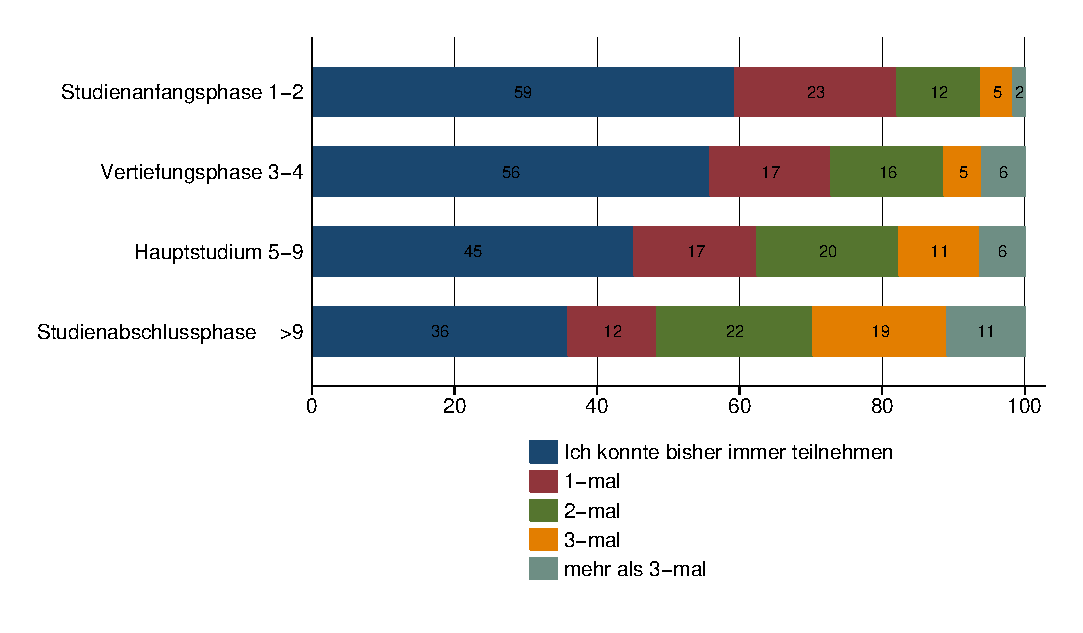
\includegraphics[
%  defaultresolution=72 !,
%  bmpsizefast=false
%]{image}
%\end{verbatim}
% \end{quote}
%
% \subsubsection{Hints}
%
% \begin{itemize}
% \item My version of \xfile{dvips.def} 1999/02/16 v3.0i defines
%       rules for the supported bitmap extensions, but does not
%       include them in the list of extensions that are tried
%       if the file name is not given with an extension.
%       In such a case, the list of extensions can be set
%       by \cs{DeclareGraphicsExtensions}, see \xpackage{grfguide}.
%       The following code just extends the list:
%       \begin{quote}
%\begin{verbatim}
%\makeatletter
%\g@addto@macro\Gin@extensions{,.bmp,.pcx,.msp}
%\makeatother
%\end{verbatim}
%       \end{quote}
% \item My version of \xfile{dvipdfm.def} 1998/11/24 vx.x misses
%       the graphics rule for PNG files. It can be added by:
%       \begin{quote}
%\begin{verbatim}
%\DeclareGraphicsRule{.png}{bmp}{.bb}{#1}
%\end{verbatim}
%       \end{quote}
%       See the previous issue to add the extension \xfile{.png} to the list
%       of extensions for package \xpackage{graphics}.
% \end{itemize}
%
% \subsubsection{Test program}
%
% There is a test program \xfile{bmpsize-test.tex}. Run it through
% \verb|latex|, \verb|pdflatex|, or \verb|pdftex|. Then given
% image files are inspected and the result is printed.
%
% \subsubsection{Interface for programmers}
%
% The macro names of the parsers are \verb|\bmpsize@read@|\meta{type}.
% Example: \cs{bmpsize@read@jpg} in case of JPEG.
%
% A parser sets the switch \cs{ifbmpsize@ok} to true, if it
% could successfully parse the image file.
% The width and height are returnd in \cs{bmpsize@width} and
% \cs{bmpsize@height}. If information about density is available,
% it is used to calculate width and height of the image, otherwise
% the values given by option \xoption{defaultresolution} is used.
% \xoption{resolution} overwrites the values in the image file.
%
% \subsection{Improved bitmap inclusion}
%
% Some drivers for package \xpackage{graphics} define the graphics
% type \xoption{bmp} for bitmap images. The code in the standard
% drivers for \xoption{dvips}, \xoption{dvipdfm}, and \xoption{dvipdfmx}
% is very basic and misses essential features of the
% package \xpackage{graphicx}. Therefore the code for bitmap
% inclusion is automatically rewritten by this package to add
% the following features:
% \begin{itemize}
% \item Support for \xoption{viewport} and \xoption{trim}.
% \item Support for \xoption{clip}.
% \item In case of \xoption{dvipdfm} and \xoption{dvipdfmx} the
%       bitmap images are reused and not included again if they
%       are used more than once.
% \end{itemize}
% However, there is a difference between \xoption{dvipdfm} and
% \xoption{dvipdfmx}, especially if images are reused. In the
% former case the reused box has width and height of 1bp, in the
% latter case its natural width. Thus the correct driver option must be given.
% \xoption{dvipdfm} and \xoption{dvipdfmx} are not equivalent.
%
% Older versions of \xoption{dvipdfmx} uses a size of 1in. However I do
% want to distinguish between versions of the same program. Therefore the
% support of these older versions has stopped with version 1.6 of this package.
% Use version dvipdfmx-20090708 or newer (some few versions before will
% probably also work, but I don't want to investigate this further).
%
% \StopEventually{
% }
%
% \section{Implementation}
%
% \subsection{Basic package \xpackage{bmpsize-base}}
%
%    Identification.
%    \begin{macrocode}
%<*base>
\ProvidesPackage{bmpsize-base}%
  [2009/09/04 v1.6 Basic part of bmpsize (HO)]%
%    \end{macrocode}
%    Modules of package \xpackage{fp} are used for calculations.
%    \begin{macrocode}
\RequirePackage{fp-basic}
\RequirePackage{fp-snap}
%    \end{macrocode}
%    Package \xpackage{fp} uses nested \cs{loop} structures.
%    That breaks with the plain-\TeX\ version of \cs{loop}.
%    Therefore we use the \LaTeX\ variant.
%    \begin{macro}{\@bmpsize@plain@loop}
%    \begin{macrocode}
\long\def\@bmpsize@plain@loop#1\repeat{%
  \def\iterate{%
    #1\relax
    \expandafter\iterate\fi
  }%
  \iterate
  \let\iterate\relax
}
%    \end{macrocode}
%    \end{macro}
%    \begin{macrocode}
\RequirePackage{pdftexcmds}[2007/11/11]
%    \end{macrocode}
%    \begin{macrocode}
\newif\ifbmpsize@ok
\let\@bmpsize@ok\bmpsize@oktrue

\newif\if@bmpsize@bigendian
\newif\if@bmpsize@absnum
\newif\if@bmpsize@user@resolution
\newif\if@bmpsize@fast
\@bmpsize@fasttrue

\def\@bmpsize@init{%
  \let\@bmpsize@org@plain@loop\loop
  \let\loop\@bmpsize@plain@loop
  \bmpsize@okfalse
  \@bmpsize@bigendiantrue
  \@bmpsize@absnumfalse
  \let\bmpsize@pixelwidth\relax
  \let\bmpsize@pixelheight\relax
  \let\bmpsize@pixelx\relax
  \let\bmpsize@pixely\relax
  \let\bmpsize@unit\relax
  \let\bmpsize@pixelxdenom\relax
  \let\bmpsize@pixelydenom\relax
  \let\bmpsize@orientation\relax
}

\def\@bmpsize@stop#1\@nil{}

\def\@bmpsize@loop#1{%
  #1%
  \@bmpsize@loop{#1}%
}
\def\@bmpsize@break#1\@bmpsize@loop#2{}

\def\@bmpsize@size#1#2#3{%
  \edef#3{\pdf@filesize{#1}}%
  \ifx#3\@empty
    \expandafter\@bmpsize@stop
  \fi
  \ifnum#3<#2\relax
    \expandafter\@bmpsize@stop
  \fi
}

\def\@bmpsize@read#1#2#3{%
  \edef\@bmpsize@buf{\pdf@filedump{#3}{#2}{#1}}%
  \edef\@bmpsize@temp{%
    \noexpand\@bmpsize@check@byte{#2}\@bmpsize@buf{}{}\noexpand\\%
  }%
  \@bmpsize@temp
}
\def\@bmpsize@fillbuf#1{%
  \ifx\@bmpsize@buf\@empty
    \expandafter\@firstofone
  \else
    \expandafter\@gobble
  \fi
  {%
    \edef\@bmpsize@buf{%
      \pdf@filedump{\bmpsize@offset}{\bmpsize@fillbuflength}{#1}%
    }%
    \ifx\@bmpsize@buf\@empty
      \expandafter\@bmpsize@stop
    \fi
    \edef\bmpsize@offset{\the\numexpr\bmpsize@offset+\bmpsize@fillbuflength}%
  }%
}
\def\bmpsize@fillbuflength{10}

\def\@bmpsize@append#1#2#3{%
  \edef#1{#2#3}%
}
\def\@bmpsize@pushback#1{%
  \edef\@bmpsize@buf{#1\@bmpsize@buf}%
}

\def\@bmpsize@iswhite#1{%
  \ifnum\pdf@strcmp{#1}{09}=\z@
  \else
    \ifnum\pdf@strcmp{#1}{0A}=\z@
    \else
      \ifnum\pdf@strcmp{#1}{0D}=\z@
      \else
        \ifnum\pdf@strcmp{#1}{20}=\z@
        \else
          1%
        \fi
      \fi
    \fi
  \fi
  \space
}
\def\@bmpsize@isdigit#1{%
  \ifnum\pdf@strcmp{#1}{30}<\z@
    1%
  \else
    \ifnum\pdf@strcmp{#1}{39}>\z@
      1%
    \fi
  \fi
  \space
}

\def\@bmpsize@check@byte#1#2#3{%
  \ifnum#1<\@ne
    \csname fi\endcsname
    \@bmpsize@cleanup@end
  \else
    \csname fi\endcsname
  \ifx!#2#3!%
    \csname fi\endcsname
    \@bmpsize@stop
  \else
    \csname fi\endcsname
    \expandafter\@bmpsize@check@byte\expandafter{\the\numexpr#1-1}%
}
\def\@bmpsize@cleanup@end#1\\{}

\def\@bmpsize@swap@maybe#1{%
  \if@bmpsize@bigendian
  \else
    \edef#1{\expandafter\@bmpsize@@swap#1\@empty\@empty\@empty\@empty}%
  \fi
}
\def\@bmpsize@@swap#1#2#3#4#5#6#7#8{%
  #7#8#5#6#3#4#1#2%
}

\def\@bmpsize@skip@one{%
  \edef\@bmpsize@buf{\expandafter\@gobbletwo\@bmpsize@buf}%
}
\def\@bmpsize@skip@two{%
  \edef\@bmpsize@buf{\expandafter\@gobblefour\@bmpsize@buf}%
}
\def\@bmpsize@skip@four{%
  \edef\@bmpsize@buf{%
    \expandafter\expandafter\expandafter\@gobblefour\expandafter
    \@gobblefour\@bmpsize@buf
  }%
}

\def\@bmpsize@grab#1#2{%
  \edef#1{\noexpand\@bmpsize@grab@byte#2=\@bmpsize@buf\noexpand\\}%
  \edef#1{#1}%
}
\def\@bmpsize@grab@byte#1=#2#3{%
  #2#3%
  \ifnum#1>\@ne
    \expandafter\@bmpsize@grab@byte\the\numexpr#1-1\expandafter=%
  \else
    \expandafter\@bmpsize@cleanup@end
  \fi
}

\def\@bmpsize@abs@maybe#1{%
  \let\@bmpsize@temp\relax
  \if@bmpsize@absnum
    \ifnum"\expandafter\@car#1\@nil>7 %
      \edef#1{\expandafter\@bmpsize@abs@byte#1\relax}%
      \ifnum\pdf@strcmp{#1}{7FFFFFFF}=\z@
        \let\@bmpsize@temp\@bmpsize@stop
      \else
        \def\@bmpsize@temp{\edef#1{\the\numexpr#1+1}}%
      \fi
    \fi
  \fi
}
\def\@bmpsize@abs@byte#1{%
  \ifx#1\relax
  \else
    \ifcase"0#1 %
      F\or E\or D\or C\or B\or A\or 9\or 8\or
      7\or 6\or 5\or 4\or 3\or 2\or 1\or 0%
    \fi
    \expandafter\@bmpsize@abs@byte
  \fi
}

\def\@bmpsize@num@one#1{%
  \@bmpsize@grab#11%
  \@bmpsize@abs@maybe#1%
  \edef#1{\number"#1}%
  \@bmpsize@temp
  \@bmpsize@skip@one
}
\def\@bmpsize@num@two#1{%
  \@bmpsize@grab#12%
  \@bmpsize@swap@maybe#1%
  \@bmpsize@abs@maybe#1%
  \edef#1{\number"#1}%
  \@bmpsize@temp
  \@bmpsize@skip@two
}
\def\@bmpsize@num@four#1{%
  \@bmpsize@grab#14%
  \@bmpsize@swap@maybe#1%
  \@bmpsize@abs@maybe#1%
  \ifnum\pdf@strcmp{#1}{7FFFFFFF}>\z@
    \expandafter\@bmpsize@stop
  \fi
  \edef#1{\number"#1}%
  \@bmpsize@temp
  \@bmpsize@skip@four
}

\def\@bmpsize@div#1#2#3{% #1 := #2/#3
  \FPdiv#1{#2}{#3}%
  \@bmpsize@beautify#1%
}
\def\@bmpsize@beautify#1{%
  \FPifint#1%
    \edef#1{\expandafter\@bmpsize@trunc#1.\@nil}%
  \else
    \edef#1{\expandafter\@bmpsize@cleanup@frac#1.\@nil}%
  \fi
}
\def\@bmpsize@trunc#1.#2\@nil{#1}
% #1 isn't an integer, thus we should have at least one
% necessary digit after the dot
\def\@bmpsize@cleanup@frac#1.#2#3.#4\@nil{%
  #1.#2%
  \ifx\\#3\\%
  \else
    \@bmpsize@cleanup@fracdigits#3000000000\@nil
  \fi
}
\def\@bmpsize@cleanup@fracdigits#1#2#3#4#5#6#7#8#9{%
  \ifcase#9 %
    \ifcase#8 %
      \ifcase#7 %
        \ifcase#6 %
          \ifcase#5 %
            \ifcase #4 %
              \ifcase #3 %
                \ifcase #2 %
                  \ifcase #1 %
                  \else
                    #1%
                  \fi
                \else
                  #1#2%
                \fi
              \else
                #1#2#3%
              \fi
            \else
              #1#2#3#4%
            \fi
          \else
            #1#2#3#4#5%
          \fi
        \else
          #1#2#3#4#5#6%
        \fi
      \else
        #1#2#3#4#5#6#7%
      \fi
    \else
      #1#2#3#4#5#6#7#8%
    \fi
  \else
    #1#2#3#4#5#6#7#8#9%
  \fi
  \@bmpsize@trunc.%
}

\def\@bmpsize@end{%
  \ifbmpsize@ok
    \ifx\bmpsize@pixelwidth\relax
      \bmpsize@okfalse
    \fi
    \ifx\bmpsize@pixelheight\relax
      \bmpsize@okfalse
    \fi
  \fi
  \ifbmpsize@ok
    \ifnum\bmpsize@pixelwidth>\z@
    \else
      \bmpsize@okfalse
    \fi
    \ifnum\bmpsize@pixelheight>\z@
    \else
      \bmpsize@okfalse
    \fi
  \fi
  \ifbmpsize@ok
    \ifcase 0%
      \ifx\bmpsize@pixelx\relax 1 \fi
      \ifx\bmpsize@pixely\relax 1 \fi
      \ifnum\bmpsize@pixelx>\z@\else 1 \fi
      \ifnum\bmpsize@pixely>\z@\else 1 \fi
      \ifx\bmpsize@pixelxdenom\relax
         \ifx\bmpsize@pixelydenom\relax\else 1 \fi
      \else
        \ifnum\bmpsize@pixelxdenom>\z@\else 1 \fi
      \fi
      \ifx\bmpsize@pixelydenom\relax
      \else
        \ifnum\bmpsize@pixelydenom>\z@\else 1 \fi
      \fi
    \else
      \let\bmpsize@pixelx\relax
      \let\bmpsize@pixely\relax
      \let\bmpsize@unit\relax
      \let\bmpsize@pixelxdenom\relax
      \let\bmpsize@pixelydenom\relax
    \fi
    \ifx\bmpsize@pixelxdenom\relax
    \else
      \@bmpsize@div\bmpsize@pixelx\bmpsize@pixelx\bmpsize@pixelxdenom
      \@bmpsize@div\bmpsize@pixely\bmpsize@pixely\bmpsize@pixelydenom
      \let\bmpsize@pixelxdenom\relax
      \let\bmpsize@pixelydenom\relax
    \fi
    \ifcase 0\ifx\bmpsize@unit\relax 1\fi
             \if@bmpsize@user@resolution 1\fi
             \relax
      \let\bmpsize@calc@unit\bmpsize@unit
      \let\bmpsize@calc@pixelx\bmpsize@pixelx
      \let\bmpsize@calc@pixely\bmpsize@pixely
    \else
      \let\bmpsize@calc@unit\bmpsize@unit@default
      \let\bmpsize@calc@pixelx\bmpsize@pixelx@default
      \let\bmpsize@calc@pixely\bmpsize@pixely@default
      \ifx\bmpsize@calc@pixely\Gin@exclamation
        \ifx\bmpsize@pixelx\relax
          \let\bmpsize@calc@pixely\bmpsize@calc@pixelx
        \else
          \FPdiv\bmpsize@calc@pixely\bmpsize@calc@pixelx\bmpsize@pixelx
          \FPmul\bmpsize@calc@pixely\bmpsize@calc@pixely\bmpsize@pixely
        \fi
      \else
        \ifx\bmpsize@calc@pixelx\Gin@exclamation
          \ifx\bmpsize@pixelx\relax
            \let\bmpsize@calc@pixelx\bmpsize@calc@pixely
          \else
            \FPdiv\bmpsize@calc@pixelx\bmpsize@calc@pixely\bmpsize@pixely
            \FPmul\bmpsize@calc@pixelx\bmpsize@calc@pixelx\bmpsize@pixelx
          \fi
        \fi
      \fi
    \fi
    \FPdiv\bmpsize@width\bmpsize@pixelwidth\bmpsize@calc@pixelx
    \FPdiv\bmpsize@height\bmpsize@pixelheight\bmpsize@calc@pixely
    % calculation of width and height in bp for package graphics
    % 1in = 72bp = 72.27pt, 72/72.27 = 8/8.03, 1pt = 65536sp
    \if@bmpsize@fast
      \edef\bmpsize@width{%
        \strip@pt\dimexpr.99626\dimexpr
        \bmpsize@width\dimexpr\bmpsize@calc@unit
      }%
      \edef\bmpsize@height{%
        \strip@pt\dimexpr.99626\dimexpr
        \bmpsize@height\dimexpr\bmpsize@calc@unit
      }%
    \else
      \edef\@bmpsize@temp{\number\dimexpr\bmpsize@calc@unit}%
      \ifnum\@bmpsize@temp>100000 %
        \FPmul\@bmpsize@temp\@bmpsize@temp{0.00001}%
        \def\@bmpsize@corr{100000}%
      \else
        \let\@bmpsize@corr\relax
      \fi
      \FPmul\bmpsize@width\bmpsize@width\@bmpsize@temp
      \FPmul\bmpsize@height\bmpsize@height\@bmpsize@temp
      \FPmul\bmpsize@width\bmpsize@width{8}%
      \FPmul\bmpsize@height\bmpsize@height{8}%
      \FPdiv\bmpsize@width\bmpsize@width{8.03}%
      \FPdiv\bmpsize@height\bmpsize@height{8.03}%
      \FPdiv\bmpsize@width\bmpsize@width{65536}%
      \FPdiv\bmpsize@height\bmpsize@height{65536}%
      \ifx\@bmpsize@corr\relax
      \else
        \FPmul\bmpsize@width\bmpsize@width\@bmpsize@corr
        \FPmul\bmpsize@height\bmpsize@height\@bmpsize@corr
      \fi
      \FPround\bmpsize@width\bmpsize@width{5}%
      \FPround\bmpsize@height\bmpsize@height{5}%
      \@bmpsize@beautify\bmpsize@width
      \@bmpsize@beautify\bmpsize@height
    \fi
  \fi
  \let\loop\@bmpsize@org@plain@loop
}
\def\bmpsize@unit@default{72.27pt}% more accurate than 1in
\def\bmpsize@pixelx@default{72}
\let\bmpsize@pixely@default\Gin@exclamation

\def\bmpsize@types{png,jpg,bmp,gif,tiff,pnm,pam,xpm,tga,pcx,msp,sgi}
%</base>
%    \end{macrocode}
%
% \subsection{Bitmap formats}
%
% \subsubsection{png}
%
%\iffalse
%<*ignore>
%\fi
%\begin{verbatim}
%begin png
%big-endian
%
%read 24 0
%grab 8        -> $temp
%check streq $temp [0x89 "PNG" 0x0D 0x0A 0x1A 0x0A]
%num 4         -> $length
%grab 4        -> $temp
%check streq $temp ["IHDR"]
%num 4         -> $pixelwidth
%num 4         -> $pixelheight
%ok
%assign numexpr(20 + $length) -> $offset
%loop
%  read 8 $offset
%  num 4       -> $length
%  grab 4      -> $temp
%  if streq $temp ["IDAT"]
%    stop
%  fi
%  if streq $temp ["pHYs"]
%    read 9 numexpr($offset + 8)
%    num 4     -> $pixelx
%    num 4     -> $pixely
%    grab 1     -> $temp
%    if numeq $temp 1
%      assign {100cm} -> $unit
%    fi
%    stop
%  fi
%  assign numexpr($offset + 12 + $length) -> $offset
%repeat
%end
%\end{verbatim}
%\iffalse
%</ignore>
%\fi
%    \begin{macro}{\bmpsize@read@png}
%    \begin{macrocode}
%<*base>
\def\bmpsize@read@png#1{%
  \@bmpsize@init
  \@bmpsize@bigendiantrue
  \@bmpsize@read{#1}{24}{0}%
  \@bmpsize@grab\bmpsize@temp{8}%
  \@bmpsize@skip@four
  \@bmpsize@skip@four
  \ifnum\pdf@strcmp{\bmpsize@temp}{89504E470D0A1A0A}=\z@
  \else
    \expandafter\@bmpsize@stop
  \fi
  \@bmpsize@num@four\bmpsize@length
  \@bmpsize@grab\bmpsize@temp{4}%
  \@bmpsize@skip@four
  \ifnum\pdf@strcmp{\bmpsize@temp}{49484452}=\z@
  \else
    \expandafter\@bmpsize@stop
  \fi
  \@bmpsize@num@four\bmpsize@pixelwidth
  \@bmpsize@num@four\bmpsize@pixelheight
  \@bmpsize@ok
  \edef\bmpsize@offset{\the\numexpr20+\bmpsize@length}%
  \@bmpsize@loop{%
    \@bmpsize@read{#1}{8}{\bmpsize@offset}%
    \@bmpsize@num@four\bmpsize@length
    \@bmpsize@grab\bmpsize@temp{4}%
    \@bmpsize@skip@four
    \ifnum\pdf@strcmp{\bmpsize@temp}{49444154}=\z@
      \expandafter\@firstofone
    \else
      \expandafter\@gobble
    \fi
    {%
      \@bmpsize@stop
    }%
    \ifnum\pdf@strcmp{\bmpsize@temp}{70485973}=\z@
      \expandafter\@firstofone
    \else
      \expandafter\@gobble
    \fi
    {%
      \@bmpsize@read{#1}{9}{\numexpr\bmpsize@offset+8\relax}%
      \@bmpsize@num@four\bmpsize@pixelx
      \@bmpsize@num@four\bmpsize@pixely
      \@bmpsize@grab\bmpsize@temp{1}%
      \@bmpsize@skip@one
      \ifnum\bmpsize@temp=1\relax
        \expandafter\@firstofone
      \else
        \expandafter\@gobble
      \fi
      {%
        \def\bmpsize@unit{100cm}%
      }%
      \@bmpsize@stop
    }%
    \edef\bmpsize@offset{\the\numexpr\bmpsize@offset+12+\bmpsize@length}%
  }%
  \@bmpsize@stop
  \@nil
  \@bmpsize@end
}%
%</base>
%    \end{macrocode}
%    \end{macro}
%
% \subsubsection{jpg}
%
%\iffalse
%<*ignore>
%\fi
%\begin{verbatim}
%begin jpg
%
%read 3 0
%grab 3      -> $temp % SOI and 0xFF
%check streq $temp [0xFF 0xD8 0xFF]
%assign {2} -> $offset
%assign {0} -> $exifdensity
%loop
%  read 4 $offset
%  grab 1    -> $temp
%  check streq $temp [0xFF]
%  num 1    -> $temp
%  if numeq $temp 0xDA % SOS
%    stop
%  fi
%  % look for JFIF APP0 segment
%  if numeq $temp 0xE0 % APP0
%    num 2       -> $length
%    if numeq $exifdensity 0
%      if numge $length 16 % a JFIF segment has 16 bytes at least
%        read 12 numexpr($offset + 4)
%        grab 5      -> $temp % identifier
%        if streq $temp ["JFIF" 0x0]
%          check numge $length 16
%          skip 2 % version
%          num 1       -> $temp % units
%          if numeq $temp 1
%            assign {72.27pt} -> $unit
%          else
%            if numeq $temp 2
%              assign {1cm} -> $unit
%            fi
%          fi
%          num 2    -> $pixelx
%          num 2    -> $pixely
%        fi
%      fi
%    fi
%  else
%    if numeq $temp 0xE1 % APP1
%      % look for Exif APP1 segment
%      num 2 -> $length
%      if numge $length 20 % identifier (6) + Tiff header (8) + first IFD (>=6)
%        read 20 numexpr($offset + 4)
%        grab 6 -> $temp
%        if streq $temp ["Exif" 0x0 0x0]
%          assign numexpr($offset + 10) -> $exifoffset
%          % read TIFF header
%          grab 2 -> $temp
%          if streq $temp ["II"]
%            little-endian
%          else
%            check streq $temp ["MM"]
%            % big-endian
%          fi
%          num 2 -> $temp
%          check numeq $temp 42
%          num 4 -> $temp % offset of first IFD
%          check numgt $temp 0
%          % read first IFD
%          assign numexpr($temp + $exifoffset) -> $off
%          read 2 $off
%          num 2 -> $entries
%          assign numexpr($off + 2) -> $off
%          loop
%            if numeq $entries 0
%              break
%            fi
%            assign numexpr($entries - 1) -> $entries
%            % entry format:
%            % 2 tag
%            % 2 field type
%            % 4 count
%            % 4 value/offset
%            read 12 $off
%            assign numexpr($off + 12) -> $off
%            num 2 -> $tag
%            if numeq $tag 296 % ResolutionUnit
%              skip 6 % type: 3 (short), count: 1
%              num 2 -> $temp
%              ifcase $temp
%              or % 1
%                clear $unit
%              or % 2
%                assign {72.27pt} -> $unit
%              or % 3
%                assign {1cm} -> $unit
%              else
%                clear $unit % unknown
%              fi
%              ifcase $temp
%              or % 1
%              or % 2
%                assign {1} -> $exifdensity
%              or % 3
%                assign {1} -> $exifdensity
%              else
%                assign $exifdensity -> $exifdensity
%              fi
%            fi
%            % 256 ImageWidth (use width of JPG part)
%            % 257 ImageHeight (use height of JPG part)
%            if numeq $tag 274 % Orientation
%              skip 6 % type: 3 (short), count: 1
%              num 2 -> $temp
%              if numge $temp 0 
%                if numle $temp 8
%                  assign $temp -> $orientation
%                fi
%              fi
%            fi
%            if numeq $tag 282 % XResolution
%              skip 6
%              num 4 -> $temp
%              read 8 numexpr($temp + $exifoffset)
%              num 4 -> $pixelx
%              num 4 -> $temp
%              if numeq $temp 1
%              else
%                assign numexpr($temp) -> $pixelxdenom
%                % div $pixelx $temp -> $pixelx
%              fi
%            fi
%            if numeq $tag 283 % YResolution
%              skip 6
%              num 4 -> $temp
%              read 8 numexpr($temp + $exifoffset)
%              num 4 -> $pixely
%              num 4 -> $temp
%              if numeq $temp 1
%              else
%                assign numexpr($temp) -> $pixelydenom
%                % div $pixely $temp -> $pixely
%              fi
%            fi
%          repeat
%          big-endian
%        fi
%      fi
%    else
%      assign numexpr($temp - 0xC0) -> $temp
%      ifcase $temp % SOF_0
%      or % SOF_1
%      or % SOF_2
%      or % SOF_3
%      or % DHT
%        assign {-1} -> $temp
%      or % SOF_5
%      or % SOF_6
%      or % SOF_7
%      or % JPG
%        assign {-1} -> $temp
%      or % SOF_9
%      or % SOF_10
%      or % SOF_11
%      or % DAC
%        assign {-1} -> $temp
%      or % SOF_13
%      or % SOF_14
%      or % SOF_15
%      else
%        assign {-1} -> $temp
%      fi
%      if numeq $temp -1
%      else
%        read 4 numexpr($offset + 5)
%        num 2  -> $pixelheight
%        num 2  -> $pixelwidth
%        if numeq $pixelheight 0
%          clear $pixelheight
%          stop
%        fi
%        ok
%        stop
%      fi
%      num 2 -> $length
%    fi
%  fi
%  assign numexpr($offset + $length + 2) -> $offset
%repeat
%end
%\end{verbatim}
%\iffalse
%</ignore>
%\fi
%    \begin{macro}{\bmpsize@read@jpg}
%    \begin{macrocode}
%<*base>
\def\bmpsize@read@jpg#1{%
  \@bmpsize@init
  \@bmpsize@read{#1}{3}{0}%
  \@bmpsize@grab\bmpsize@temp{3}%
  \@bmpsize@skip@two
  \@bmpsize@skip@one
  \ifnum\pdf@strcmp{\bmpsize@temp}{FFD8FF}=\z@
  \else
    \expandafter\@bmpsize@stop
  \fi
  \def\bmpsize@offset{2}%
  \def\bmpsize@exifdensity{0}%
  \@bmpsize@loop{%
    \@bmpsize@read{#1}{4}{\bmpsize@offset}%
    \@bmpsize@grab\bmpsize@temp{1}%
    \@bmpsize@skip@one
    \ifnum\pdf@strcmp{\bmpsize@temp}{FF}=\z@
    \else
      \expandafter\@bmpsize@stop
    \fi
    \@bmpsize@num@one\bmpsize@temp
    \ifnum\bmpsize@temp=218\relax
      \expandafter\@firstofone
    \else
      \expandafter\@gobble
    \fi
    {%
      \@bmpsize@stop
    }%
    \ifnum\bmpsize@temp=224\relax
      \expandafter\@firstoftwo
    \else
      \expandafter\@secondoftwo
    \fi
    {%
      \@bmpsize@num@two\bmpsize@length
      \ifnum\bmpsize@exifdensity=0\relax
        \expandafter\@firstofone
      \else
        \expandafter\@gobble
      \fi
      {%
        \unless\ifnum\bmpsize@length<16\relax
          \expandafter\@firstofone
        \else
          \expandafter\@gobble
        \fi
        {%
          \@bmpsize@read{#1}{12}{\numexpr\bmpsize@offset+4\relax}%
          \@bmpsize@grab\bmpsize@temp{5}%
          \@bmpsize@skip@four
          \@bmpsize@skip@one
          \ifnum\pdf@strcmp{\bmpsize@temp}{4A46494600}=\z@
            \expandafter\@firstofone
          \else
            \expandafter\@gobble
          \fi
          {%
            \ifnum\bmpsize@length<16\relax
              \expandafter\@bmpsize@stop
            \fi
            \@bmpsize@skip@two
            \@bmpsize@num@one\bmpsize@temp
            \ifnum\bmpsize@temp=1\relax
              \expandafter\@firstoftwo
            \else
              \expandafter\@secondoftwo
            \fi
            {%
              \def\bmpsize@unit{72.27pt}%
            }{%
              \ifnum\bmpsize@temp=2\relax
                \expandafter\@firstofone
              \else
                \expandafter\@gobble
              \fi
              {%
                \def\bmpsize@unit{1cm}%
              }%
            }%
            \@bmpsize@num@two\bmpsize@pixelx
            \@bmpsize@num@two\bmpsize@pixely
          }%
        }%
      }%
    }{%
      \ifnum\bmpsize@temp=225\relax
        \expandafter\@firstoftwo
      \else
        \expandafter\@secondoftwo
      \fi
      {%
        \@bmpsize@num@two\bmpsize@length
        \unless\ifnum\bmpsize@length<20\relax
          \expandafter\@firstofone
        \else
          \expandafter\@gobble
        \fi
        {%
          \@bmpsize@read{#1}{20}{\numexpr\bmpsize@offset+4\relax}%
          \@bmpsize@grab\bmpsize@temp{6}%
          \@bmpsize@skip@four
          \@bmpsize@skip@two
          \ifnum\pdf@strcmp{\bmpsize@temp}{457869660000}=\z@
            \expandafter\@firstofone
          \else
            \expandafter\@gobble
          \fi
          {%
            \edef\bmpsize@exifoffset{\the\numexpr\bmpsize@offset+10}%
            \@bmpsize@grab\bmpsize@temp{2}%
            \@bmpsize@skip@two
            \ifnum\pdf@strcmp{\bmpsize@temp}{4949}=\z@
              \expandafter\@firstoftwo
            \else
              \expandafter\@secondoftwo
            \fi
            {%
              \@bmpsize@bigendianfalse
            }{%
              \ifnum\pdf@strcmp{\bmpsize@temp}{4D4D}=\z@
              \else
                \expandafter\@bmpsize@stop
              \fi
            }%
            \@bmpsize@num@two\bmpsize@temp
            \ifnum\bmpsize@temp=42\relax
            \else
              \expandafter\@bmpsize@stop
            \fi
            \@bmpsize@num@four\bmpsize@temp
            \ifnum\bmpsize@temp>0\relax
            \else
              \expandafter\@bmpsize@stop
            \fi
            \edef\bmpsize@off{\the\numexpr\bmpsize@temp+\bmpsize@exifoffset}%
            \@bmpsize@read{#1}{2}{\bmpsize@off}%
            \@bmpsize@num@two\bmpsize@entries
            \edef\bmpsize@off{\the\numexpr\bmpsize@off+2}%
            \@bmpsize@loop{%
              \ifnum\bmpsize@entries=0\relax
                \expandafter\@firstofone
              \else
                \expandafter\@gobble
              \fi
              {%
                \@bmpsize@break
              }%
              \edef\bmpsize@entries{\the\numexpr\bmpsize@entries-1}%
              \@bmpsize@read{#1}{12}{\bmpsize@off}%
              \edef\bmpsize@off{\the\numexpr\bmpsize@off+12}%
              \@bmpsize@num@two\bmpsize@tag
              \ifnum\bmpsize@tag=296\relax
                \expandafter\@firstofone
              \else
                \expandafter\@gobble
              \fi
              {%
                \@bmpsize@skip@four
                \@bmpsize@skip@two
                \@bmpsize@num@two\bmpsize@temp
                \ifcase\bmpsize@temp\relax
                \or
                  \let\bmpsize@unit\relax
                \or
                  \def\bmpsize@unit{72.27pt}%
                \or
                  \def\bmpsize@unit{1cm}%
                \else
                  \let\bmpsize@unit\relax
                \fi
                \ifcase\bmpsize@temp\relax
                \or
                \or
                  \def\bmpsize@exifdensity{1}%
                \or
                  \def\bmpsize@exifdensity{1}%
                \else
                  \let\bmpsize@exifdensity\bmpsize@exifdensity
                \fi
              }%
              \ifnum\bmpsize@tag=274\relax
                \expandafter\@firstofone
              \else
                \expandafter\@gobble
              \fi
              {%
                \@bmpsize@skip@four
                \@bmpsize@skip@two
                \@bmpsize@num@two\bmpsize@temp
                \unless\ifnum\bmpsize@temp<0\relax
                  \expandafter\@firstofone
                \else
                  \expandafter\@gobble
                \fi
                {%
                  \unless\ifnum\bmpsize@temp>8\relax
                    \expandafter\@firstofone
                  \else
                    \expandafter\@gobble
                  \fi
                  {%
                    \let\bmpsize@orientation\bmpsize@temp
                  }%
                }%
              }%
              \ifnum\bmpsize@tag=282\relax
                \expandafter\@firstofone
              \else
                \expandafter\@gobble
              \fi
              {%
                \@bmpsize@skip@four
                \@bmpsize@skip@two
                \@bmpsize@num@four\bmpsize@temp
                \@bmpsize@read{#1}{8}{\numexpr\bmpsize@temp+\bmpsize@exifoffset\relax}%
                \@bmpsize@num@four\bmpsize@pixelx
                \@bmpsize@num@four\bmpsize@temp
                \ifnum\bmpsize@temp=1\relax
                  \expandafter\@gobble
                \else
                  \expandafter\@firstofone
                \fi
                {%
                  \edef\bmpsize@pixelxdenom{\the\numexpr\bmpsize@temp}%
                }%
              }%
              \ifnum\bmpsize@tag=283\relax
                \expandafter\@firstofone
              \else
                \expandafter\@gobble
              \fi
              {%
                \@bmpsize@skip@four
                \@bmpsize@skip@two
                \@bmpsize@num@four\bmpsize@temp
                \@bmpsize@read{#1}{8}{\numexpr\bmpsize@temp+\bmpsize@exifoffset\relax}%
                \@bmpsize@num@four\bmpsize@pixely
                \@bmpsize@num@four\bmpsize@temp
                \ifnum\bmpsize@temp=1\relax
                  \expandafter\@gobble
                \else
                  \expandafter\@firstofone
                \fi
                {%
                  \edef\bmpsize@pixelydenom{\the\numexpr\bmpsize@temp}%
                }%
              }%
            }%
            \@bmpsize@bigendiantrue
          }%
        }%
      }{%
        \edef\bmpsize@temp{\the\numexpr\bmpsize@temp-192}%
        \ifcase\bmpsize@temp\relax
        \or
        \or
        \or
        \or
          \def\bmpsize@temp{-1}%
        \or
        \or
        \or
        \or
          \def\bmpsize@temp{-1}%
        \or
        \or
        \or
        \or
          \def\bmpsize@temp{-1}%
        \or
        \or
        \or
        \else
          \def\bmpsize@temp{-1}%
        \fi
        \ifnum\bmpsize@temp=-1\relax
          \expandafter\@gobble
        \else
          \expandafter\@firstofone
        \fi
        {%
          \@bmpsize@read{#1}{4}{\numexpr\bmpsize@offset+5\relax}%
          \@bmpsize@num@two\bmpsize@pixelheight
          \@bmpsize@num@two\bmpsize@pixelwidth
          \ifnum\bmpsize@pixelheight=0\relax
            \expandafter\@firstofone
          \else
            \expandafter\@gobble
          \fi
          {%
            \let\bmpsize@pixelheight\relax
            \@bmpsize@stop
          }%
          \@bmpsize@ok
          \@bmpsize@stop
        }%
        \@bmpsize@num@two\bmpsize@length
      }%
    }%
    \edef\bmpsize@offset{\the\numexpr\bmpsize@offset+\bmpsize@length+2}%
  }%
  \@bmpsize@stop
  \@nil
  \@bmpsize@end
}%
%</base>
%    \end{macrocode}
%    \end{macro}
%
% \subsubsection{bmp}
%
%\iffalse
%<*ignore>
%\fi
%\begin{verbatim}
%begin bmp
%little-endian
%
%read 26 0
%grab 2 -> $temp
%check streq $temp ["BM"]
%skip 12
%% header size is 4 bytes in V3+, unknown for V1, V2,
%% known header sizes fit in 2 bytes
%num 2   -> $temp
%if numeq $temp 12 % V1
%  skip 2
%  num 2 -> $pixelwidth
%  num 2 -> $pixelheight
%  % no resolution entries
%  ok
%  stop
%fi
%if numeq $temp 64 % V2
%  skip 2
%  num 2 -> $pixelwidth
%  num 2 -> $pixelheight
%  % missing specification for resolution
%  ok
%  stop
%fi
%% V3, V4, V5
%skip 2
%num 4 -> $pixelwidth
%absnum 4 -> $pixelheight
%ok
%read 8 38
%num 4 -> $pixelx
%num 4 -> $pixely
%assign {100cm} -> $unit
%end
%\end{verbatim}
%\iffalse
%</ignore>
%\fi
%    \begin{macro}{\bmpsize@read@bmp}
%    \begin{macrocode}
%<*base>
\def\bmpsize@read@bmp#1{%
  \@bmpsize@init
  \@bmpsize@bigendianfalse
  \@bmpsize@read{#1}{26}{0}%
  \@bmpsize@grab\bmpsize@temp{2}%
  \@bmpsize@skip@two
  \ifnum\pdf@strcmp{\bmpsize@temp}{424D}=\z@
  \else
    \expandafter\@bmpsize@stop
  \fi
  \@bmpsize@skip@four
  \@bmpsize@skip@four
  \@bmpsize@skip@four
  \@bmpsize@num@two\bmpsize@temp
  \ifnum\bmpsize@temp=12\relax
    \expandafter\@firstofone
  \else
    \expandafter\@gobble
  \fi
  {%
    \@bmpsize@skip@two
    \@bmpsize@num@two\bmpsize@pixelwidth
    \@bmpsize@num@two\bmpsize@pixelheight
    \@bmpsize@ok
    \@bmpsize@stop
  }%
  \ifnum\bmpsize@temp=64\relax
    \expandafter\@firstofone
  \else
    \expandafter\@gobble
  \fi
  {%
    \@bmpsize@skip@two
    \@bmpsize@num@two\bmpsize@pixelwidth
    \@bmpsize@num@two\bmpsize@pixelheight
    \@bmpsize@ok
    \@bmpsize@stop
  }%
  \@bmpsize@skip@two
  \@bmpsize@num@four\bmpsize@pixelwidth
  \@bmpsize@absnumtrue
  \@bmpsize@num@four\bmpsize@pixelheight
  \@bmpsize@absnumfalse
  \@bmpsize@ok
  \@bmpsize@read{#1}{8}{38}%
  \@bmpsize@num@four\bmpsize@pixelx
  \@bmpsize@num@four\bmpsize@pixely
  \def\bmpsize@unit{100cm}%
  \@bmpsize@stop
  \@nil
  \@bmpsize@end
}%
%</base>
%    \end{macrocode}
%    \end{macro}
%
% \subsubsection{gif}
%
%\iffalse
%<*ignore>
%\fi
%\begin{verbatim}
%begin gif
%little-endian
%
%% Header
%read 13 0
%grab 3      -> $temp
%check streq $temp ["GIF"]
%skip 3      % version
%
%% Logical Screen Descriptor
%num 2       -> $pixelwidth
%num 2       -> $pixelheight
%skip 2
%num 1       -> $temp % Pixel Aspect Ratio
%if numeq $temp 0
%else
%  assign numexpr($temp + 15) -> $pixelx
%  assign {64}     -> $pixely
%fi
%ok
%end
%\end{verbatim}
%\iffalse
%</ignore>
%\fi
%    \begin{macro}{\bmpsize@read@gif}
%    \begin{macrocode}
%<*base>
\def\bmpsize@read@gif#1{%
  \@bmpsize@init
  \@bmpsize@bigendianfalse
  \@bmpsize@read{#1}{13}{0}%
  \@bmpsize@grab\bmpsize@temp{3}%
  \@bmpsize@skip@two
  \@bmpsize@skip@one
  \ifnum\pdf@strcmp{\bmpsize@temp}{474946}=\z@
  \else
    \expandafter\@bmpsize@stop
  \fi
  \@bmpsize@skip@two
  \@bmpsize@skip@one
  \@bmpsize@num@two\bmpsize@pixelwidth
  \@bmpsize@num@two\bmpsize@pixelheight
  \@bmpsize@skip@two
  \@bmpsize@num@one\bmpsize@temp
  \ifnum\bmpsize@temp=0\relax
    \expandafter\@gobble
  \else
    \expandafter\@firstofone
  \fi
  {%
    \edef\bmpsize@pixelx{\the\numexpr\bmpsize@temp+15}%
    \def\bmpsize@pixely{64}%
  }%
  \@bmpsize@ok
  \@bmpsize@stop
  \@nil
  \@bmpsize@end
}%
%</base>
%    \end{macrocode}
%    \end{macro}
%
% \subsubsection{tiff}
%
%\iffalse
%<*ignore>
%\fi
%\begin{verbatim}
%begin tiff
%% defaults
%assign {72.27pt} -> $unit
%
%% Image File Header
%read 8 0
%grab 2 -> $temp
%if streq $temp ["II"]
%  little-endian
%else
%  check streq $temp ["MM"]
%  big-endian
%fi
%num 2 -> $temp
%check numeq $temp 42
%num 4 -> $offset % first IFD (Image File Directory)
%
%% First IFD
%read 2 $offset
%assign numexpr($offset + 2) -> $offset
%num 2 -> $entries
%ok % must rely on checks at the end
%loop
%  if numeq $entries 0
%    stop
%  fi
%  assign numexpr($entries - 1) -> $entries
%  % entry format:
%  % 2 tag
%  % 2 field type
%  % 4 count
%  % 4 value/offset
%  read 12 $offset
%  assign numexpr($offset + 12) -> $offset
%  num 2 -> $tag % tag
%  if numeq $temp 296 % ResolutionUnit
%    skip 6 % type: 3 (short), count: 1
%    num 2 -> $temp
%    ifcase $temp
%    or % 1
%      clear $unit
%    or % 2
%      assign {72.27pt} -> $unit
%    or % 3
%      assign {1cm} -> $unit
%    else
%      clear $unit
%    fi
%  fi
%  if numeq $tag 256 % ImageWidth
%    skip 6
%    num 4 -> $pixelwidth
%  fi
%  if numeq $tag 257 % ImageLength
%    skip 6
%    num 4 -> $pixelheight
%  fi
%  if numeq $tag 282 % XResolution
%    skip 6
%    num 4 -> $temp
%    read 8 $temp
%    num 4 -> $pixelx
%    num 4 -> $temp
%    if numeq $temp 1
%    else
%      assign numexpr($temp) -> $pixelxdenom
%      % div $pixelx $temp -> $pixelx
%    fi
%  fi
%  if numeq $tag 283 % YResolution
%    skip 6
%    num 4 -> $temp
%    read 8 $temp
%    num 4 -> $pixely
%    num 4 -> $temp
%    if numeq $temp 1
%    else
%      assign numexpr($temp) -> $pixelydenom
%      % div $pixely $temp -> $pixely
%    fi
%  fi
%repeat
%end
%\end{verbatim}
%\iffalse
%</ignore>
%\fi
%    \begin{macro}{\bmpsize@read@tiff}
%    \begin{macrocode}
%<*base>
\def\bmpsize@read@tiff#1{%
  \@bmpsize@init
  \def\bmpsize@unit{72.27pt}%
  \@bmpsize@read{#1}{8}{0}%
  \@bmpsize@grab\bmpsize@temp{2}%
  \@bmpsize@skip@two
  \ifnum\pdf@strcmp{\bmpsize@temp}{4949}=\z@
    \expandafter\@firstoftwo
  \else
    \expandafter\@secondoftwo
  \fi
  {%
    \@bmpsize@bigendianfalse
  }{%
    \ifnum\pdf@strcmp{\bmpsize@temp}{4D4D}=\z@
    \else
      \expandafter\@bmpsize@stop
    \fi
    \@bmpsize@bigendiantrue
  }%
  \@bmpsize@num@two\bmpsize@temp
  \ifnum\bmpsize@temp=42\relax
  \else
    \expandafter\@bmpsize@stop
  \fi
  \@bmpsize@num@four\bmpsize@offset
  \@bmpsize@read{#1}{2}{\bmpsize@offset}%
  \edef\bmpsize@offset{\the\numexpr\bmpsize@offset+2}%
  \@bmpsize@num@two\bmpsize@entries
  \@bmpsize@ok
  \@bmpsize@loop{%
    \ifnum\bmpsize@entries=0\relax
      \expandafter\@firstofone
    \else
      \expandafter\@gobble
    \fi
    {%
      \@bmpsize@stop
    }%
    \edef\bmpsize@entries{\the\numexpr\bmpsize@entries-1}%
    \@bmpsize@read{#1}{12}{\bmpsize@offset}%
    \edef\bmpsize@offset{\the\numexpr\bmpsize@offset+12}%
    \@bmpsize@num@two\bmpsize@tag
    \ifnum\bmpsize@temp=296\relax
      \expandafter\@firstofone
    \else
      \expandafter\@gobble
    \fi
    {%
      \@bmpsize@skip@four
      \@bmpsize@skip@two
      \@bmpsize@num@two\bmpsize@temp
      \ifcase\bmpsize@temp\relax
      \or
        \let\bmpsize@unit\relax
      \or
        \def\bmpsize@unit{72.27pt}%
      \or
        \def\bmpsize@unit{1cm}%
      \else
        \let\bmpsize@unit\relax
      \fi
    }%
    \ifnum\bmpsize@tag=256\relax
      \expandafter\@firstofone
    \else
      \expandafter\@gobble
    \fi
    {%
      \@bmpsize@skip@four
      \@bmpsize@skip@two
      \@bmpsize@num@four\bmpsize@pixelwidth
    }%
    \ifnum\bmpsize@tag=257\relax
      \expandafter\@firstofone
    \else
      \expandafter\@gobble
    \fi
    {%
      \@bmpsize@skip@four
      \@bmpsize@skip@two
      \@bmpsize@num@four\bmpsize@pixelheight
    }%
    \ifnum\bmpsize@tag=282\relax
      \expandafter\@firstofone
    \else
      \expandafter\@gobble
    \fi
    {%
      \@bmpsize@skip@four
      \@bmpsize@skip@two
      \@bmpsize@num@four\bmpsize@temp
      \@bmpsize@read{#1}{8}{\bmpsize@temp}%
      \@bmpsize@num@four\bmpsize@pixelx
      \@bmpsize@num@four\bmpsize@temp
      \ifnum\bmpsize@temp=1\relax
        \expandafter\@gobble
      \else
        \expandafter\@firstofone
      \fi
      {%
        \edef\bmpsize@pixelxdenom{\the\numexpr\bmpsize@temp}%
      }%
    }%
    \ifnum\bmpsize@tag=283\relax
      \expandafter\@firstofone
    \else
      \expandafter\@gobble
    \fi
    {%
      \@bmpsize@skip@four
      \@bmpsize@skip@two
      \@bmpsize@num@four\bmpsize@temp
      \@bmpsize@read{#1}{8}{\bmpsize@temp}%
      \@bmpsize@num@four\bmpsize@pixely
      \@bmpsize@num@four\bmpsize@temp
      \ifnum\bmpsize@temp=1\relax
        \expandafter\@gobble
      \else
        \expandafter\@firstofone
      \fi
      {%
        \edef\bmpsize@pixelydenom{\the\numexpr\bmpsize@temp}%
      }%
    }%
  }%
  \@bmpsize@stop
  \@nil
  \@bmpsize@end
}%
%</base>
%    \end{macrocode}
%    \end{macro}
%
% \subsubsection{pnm}
%
%\iffalse
%<*ignore>
%\fi
%\begin{verbatim}
%begin pnm
%assign {0} -> $offset
%read 3 $offset
%assign {3} -> $offset
%grab 1 -> $temp
%check streq $temp ["P"]
%grab 1 -> $temp
%check strge $temp ["1"]
%check strle $temp ["6"]
%% ensure one white space
%grab 1 -> $temp
%if iswhite $temp
%else
%  stop
%fi
%loop
%  % skip white space
%  fillbuf
%  grab 1 -> $temp
%  if iswhite $temp
%  else
%    if streq $temp ["#"]
%      % ignore comments
%      loop
%        fillbuf
%        grab 1 -> $temp
%        if streq $temp [0x0A]
%          break
%        else
%          if streq $temp [0x0D]
%            break
%          fi
%        fi
%      repeat
%    else
%      pushback $temp
%      break
%    fi
%  fi
%repeat
%assign {} -> $tempnum
%loop
%  fillbuf
%  grab 1 -> $temp
%  if isdigit $temp
%    append $tempnum $temp -> $tempnum
%  else
%    if iswhite $temp
%      break
%    else
%      stop
%    fi
%  fi
%repeat
%assign unescapehex($tempnum) -> $pixelwidth
%loop
%  fillbuf
%  grab 1 -> $temp
%  if iswhite $temp
%  else
%    pushback $temp
%    break
%  fi
%repeat
%assign {} -> $tempnum
%loop
%  fillbuf
%  grab 1 -> $temp
%  if isdigit $temp
%    append $tempnum $temp -> $tempnum
%  else
%    if iswhite $temp
%      break
%    else
%      stop
%    fi
%  fi
%repeat
%assign unescapehex($tempnum) -> $pixelheight
%ok
%end
%\end{verbatim}
%\iffalse
%</ignore>
%\fi
%    \begin{macro}{\bmpsize@read@pnm}
%    \begin{macrocode}
%<*base>
\def\bmpsize@read@pnm#1{%
  \@bmpsize@init
  \def\bmpsize@offset{0}%
  \@bmpsize@read{#1}{3}{\bmpsize@offset}%
  \def\bmpsize@offset{3}%
  \@bmpsize@grab\bmpsize@temp{1}%
  \@bmpsize@skip@one
  \ifnum\pdf@strcmp{\bmpsize@temp}{50}=\z@
  \else
    \expandafter\@bmpsize@stop
  \fi
  \@bmpsize@grab\bmpsize@temp{1}%
  \@bmpsize@skip@one
  \ifnum\pdf@strcmp{\bmpsize@temp}{31}<\z@
    \expandafter\@bmpsize@stop
  \fi
  \ifnum\pdf@strcmp{\bmpsize@temp}{36}>\z@
    \expandafter\@bmpsize@stop
  \fi
  \@bmpsize@grab\bmpsize@temp{1}%
  \@bmpsize@skip@one
  \ifcase 0\@bmpsize@iswhite\bmpsize@temp
    \expandafter\@gobble
  \else
    \expandafter\@firstofone
  \fi
  {%
    \@bmpsize@stop
  }%
  \@bmpsize@loop{%
    \@bmpsize@fillbuf{#1}%
    \@bmpsize@grab\bmpsize@temp{1}%
    \@bmpsize@skip@one
    \ifcase 0\@bmpsize@iswhite\bmpsize@temp
      \expandafter\@gobble
    \else
      \expandafter\@firstofone
    \fi
    {%
      \ifnum\pdf@strcmp{\bmpsize@temp}{23}=\z@
        \expandafter\@firstoftwo
      \else
        \expandafter\@secondoftwo
      \fi
      {%
        \@bmpsize@loop{%
          \@bmpsize@fillbuf{#1}%
          \@bmpsize@grab\bmpsize@temp{1}%
          \@bmpsize@skip@one
          \ifnum\pdf@strcmp{\bmpsize@temp}{0A}=\z@
            \expandafter\@firstoftwo
          \else
            \expandafter\@secondoftwo
          \fi
          {%
            \@bmpsize@break
          }{%
            \ifnum\pdf@strcmp{\bmpsize@temp}{0D}=\z@
              \expandafter\@firstofone
            \else
              \expandafter\@gobble
            \fi
            {%
              \@bmpsize@break
            }%
          }%
        }%
      }{%
        \@bmpsize@pushback\bmpsize@temp
        \@bmpsize@break
      }%
    }%
  }%
  \def\bmpsize@tempnum{}%
  \@bmpsize@loop{%
    \@bmpsize@fillbuf{#1}%
    \@bmpsize@grab\bmpsize@temp{1}%
    \@bmpsize@skip@one
    \ifcase 0\@bmpsize@isdigit\bmpsize@temp
      \expandafter\@firstoftwo
    \else
      \expandafter\@secondoftwo
    \fi
    {%
      \@bmpsize@append\bmpsize@tempnum\bmpsize@tempnum\bmpsize@temp
    }{%
      \ifcase 0\@bmpsize@iswhite\bmpsize@temp
        \expandafter\@firstoftwo
      \else
        \expandafter\@secondoftwo
      \fi
      {%
        \@bmpsize@break
      }{%
        \@bmpsize@stop
      }%
    }%
  }%
  \edef\bmpsize@pixelwidth{\pdf@unescapehex{\bmpsize@tempnum}}%
  \@bmpsize@loop{%
    \@bmpsize@fillbuf{#1}%
    \@bmpsize@grab\bmpsize@temp{1}%
    \@bmpsize@skip@one
    \ifcase 0\@bmpsize@iswhite\bmpsize@temp
      \expandafter\@gobble
    \else
      \expandafter\@firstofone
    \fi
    {%
      \@bmpsize@pushback\bmpsize@temp
      \@bmpsize@break
    }%
  }%
  \def\bmpsize@tempnum{}%
  \@bmpsize@loop{%
    \@bmpsize@fillbuf{#1}%
    \@bmpsize@grab\bmpsize@temp{1}%
    \@bmpsize@skip@one
    \ifcase 0\@bmpsize@isdigit\bmpsize@temp
      \expandafter\@firstoftwo
    \else
      \expandafter\@secondoftwo
    \fi
    {%
      \@bmpsize@append\bmpsize@tempnum\bmpsize@tempnum\bmpsize@temp
    }{%
      \ifcase 0\@bmpsize@iswhite\bmpsize@temp
        \expandafter\@firstoftwo
      \else
        \expandafter\@secondoftwo
      \fi
      {%
        \@bmpsize@break
      }{%
        \@bmpsize@stop
      }%
    }%
  }%
  \edef\bmpsize@pixelheight{\pdf@unescapehex{\bmpsize@tempnum}}%
  \@bmpsize@ok
  \@bmpsize@stop
  \@nil
  \@bmpsize@end
}%
%</base>
%    \end{macrocode}
%    \end{macro}
%
% \subsubsection{pam}
%
%\iffalse
%<*ignore>
%\fi
%\begin{verbatim}
%begin pam
%read 3 0
%assign {3} -> $offset
%assign $offset -> $off
%grab 3 -> $temp
%check streq $temp ["P7" 0x0A]
%loop
%  fillbuf
%  grab 1 -> $temp
%  if iswhite $temp
%    % ignore white space
%    assign numexpr($off + 1) -> $off
%  else
%    if streq $temp ["#"]
%      % ignore comment line
%      assign numexpr($off + 1) -> $off
%      loop
%        fillbuf
%        grab 1 -> $temp
%        assign numexpr($off + 1) -> $off
%        if streq $temp [0x0A]
%          break
%        fi
%      repeat
%    else
%      read 6 $off
%      assign numexpr($off + 6) -> $offset
%      grab 5 -> $head
%      if streq $head ["WIDTH"]
%        assign numexpr($off + 5) -> $off
%        % skip white space
%        loop
%          fillbuf
%          grab 1 -> $temp
%          if iswhite $temp
%            assign numexpr($off + 1) -> $off
%          else
%            if isdigit $temp
%              assign numexpr($off + 1) -> $off
%              break
%            else
%              % error
%              stop
%            fi
%          fi
%        repeat
%        % read number
%        assign $temp -> $tempnum
%        loop
%          fillbuf
%          grab 1 -> $temp
%          if isdigit $temp
%            assign numexpr($off + 1) -> $off
%            append $tempnum $temp -> $tempnum
%          else
%            pushback $temp
%            break
%          fi
%        repeat
%        % skip to end of line
%        loop
%          fillbuf
%          grab 1 -> $temp
%          assign numexpr($off + 1) -> $off
%          if streq $temp [0x0A]
%            break
%          fi
%        repeat
%        assign unescapehex($tempnum) -> $pixelwidth
%      else
%        grab 1 -> $temp
%        append $head $temp -> $head
%        if streq $head ["ENDHDR"]
%          % last header line
%          ok
%          stop
%        else
%          if streq $head ["HEIGHT"]
%            assign numexpr($off + 6) -> $off
%            % skip white space
%            loop
%              fillbuf
%              grab 1 -> $temp
%              if iswhite $temp
%                assign numexpr($off + 1) -> $off
%              else
%                if isdigit $temp
%                  assign numexpr($off + 1) -> $off
%                  break
%                else
%                  % error
%                  stop
%                fi
%              fi
%            repeat
%            % read number
%            assign $temp -> $tempnum
%            loop
%              fillbuf
%              grab 1 -> $temp
%              if isdigit $temp
%                assign numexpr($off + 1) -> $off
%                append $tempnum $temp -> $tempnum
%              else
%                pushback $temp
%                break
%              fi
%            repeat
%            % skip to end of line
%            loop
%              fillbuf
%              grab 1 -> $temp
%              assign numexpr($off + 1) -> $off
%              if streq $temp [0x0A]
%                break
%              fi
%            repeat
%            assign unescapehex($tempnum) -> $pixelheight
%          else
%            % ignore unknown header line
%            pushback $head
%            loop
%              fillbuf
%              grab 1 -> $temp
%              assign numexpr($off + 1) -> $off
%              if streq $temp [0x0A]
%                break
%              fi
%            repeat
%          fi
%        fi
%      fi
%    fi
%  fi
%repeat
%end
%\end{verbatim}
%\iffalse
%</ignore>
%\fi
%    \begin{macro}{\bmpsize@read@pam}
%    \begin{macrocode}
%<*base>
\def\bmpsize@read@pam#1{%
  \@bmpsize@init
  \@bmpsize@read{#1}{3}{0}%
  \def\bmpsize@offset{3}%
  \let\bmpsize@off\bmpsize@offset
  \@bmpsize@grab\bmpsize@temp{3}%
  \@bmpsize@skip@two
  \@bmpsize@skip@one
  \ifnum\pdf@strcmp{\bmpsize@temp}{50370A}=\z@
  \else
    \expandafter\@bmpsize@stop
  \fi
  \@bmpsize@loop{%
    \@bmpsize@fillbuf{#1}%
    \@bmpsize@grab\bmpsize@temp{1}%
    \@bmpsize@skip@one
    \ifcase 0\@bmpsize@iswhite\bmpsize@temp
      \expandafter\@firstoftwo
    \else
      \expandafter\@secondoftwo
    \fi
    {%
      \edef\bmpsize@off{\the\numexpr\bmpsize@off+1}%
    }{%
      \ifnum\pdf@strcmp{\bmpsize@temp}{23}=\z@
        \expandafter\@firstoftwo
      \else
        \expandafter\@secondoftwo
      \fi
      {%
        \edef\bmpsize@off{\the\numexpr\bmpsize@off+1}%
        \@bmpsize@loop{%
          \@bmpsize@fillbuf{#1}%
          \@bmpsize@grab\bmpsize@temp{1}%
          \@bmpsize@skip@one
          \edef\bmpsize@off{\the\numexpr\bmpsize@off+1}%
          \ifnum\pdf@strcmp{\bmpsize@temp}{0A}=\z@
            \expandafter\@firstofone
          \else
            \expandafter\@gobble
          \fi
          {%
            \@bmpsize@break
          }%
        }%
      }{%
        \@bmpsize@read{#1}{6}{\bmpsize@off}%
        \edef\bmpsize@offset{\the\numexpr\bmpsize@off+6}%
        \@bmpsize@grab\bmpsize@head{5}%
        \@bmpsize@skip@four
        \@bmpsize@skip@one
        \ifnum\pdf@strcmp{\bmpsize@head}{5749445448}=\z@
          \expandafter\@firstoftwo
        \else
          \expandafter\@secondoftwo
        \fi
        {%
          \edef\bmpsize@off{\the\numexpr\bmpsize@off+5}%
          \@bmpsize@loop{%
            \@bmpsize@fillbuf{#1}%
            \@bmpsize@grab\bmpsize@temp{1}%
            \@bmpsize@skip@one
            \ifcase 0\@bmpsize@iswhite\bmpsize@temp
              \expandafter\@firstoftwo
            \else
              \expandafter\@secondoftwo
            \fi
            {%
              \edef\bmpsize@off{\the\numexpr\bmpsize@off+1}%
            }{%
              \ifcase 0\@bmpsize@isdigit\bmpsize@temp
                \expandafter\@firstoftwo
              \else
                \expandafter\@secondoftwo
              \fi
              {%
                \edef\bmpsize@off{\the\numexpr\bmpsize@off+1}%
                \@bmpsize@break
              }{%
                \@bmpsize@stop
              }%
            }%
          }%
          \let\bmpsize@tempnum\bmpsize@temp
          \@bmpsize@loop{%
            \@bmpsize@fillbuf{#1}%
            \@bmpsize@grab\bmpsize@temp{1}%
            \@bmpsize@skip@one
            \ifcase 0\@bmpsize@isdigit\bmpsize@temp
              \expandafter\@firstoftwo
            \else
              \expandafter\@secondoftwo
            \fi
            {%
              \edef\bmpsize@off{\the\numexpr\bmpsize@off+1}%
              \@bmpsize@append\bmpsize@tempnum\bmpsize@tempnum\bmpsize@temp
            }{%
              \@bmpsize@pushback\bmpsize@temp
              \@bmpsize@break
            }%
          }%
          \@bmpsize@loop{%
            \@bmpsize@fillbuf{#1}%
            \@bmpsize@grab\bmpsize@temp{1}%
            \@bmpsize@skip@one
            \edef\bmpsize@off{\the\numexpr\bmpsize@off+1}%
            \ifnum\pdf@strcmp{\bmpsize@temp}{0A}=\z@
              \expandafter\@firstofone
            \else
              \expandafter\@gobble
            \fi
            {%
              \@bmpsize@break
            }%
          }%
          \edef\bmpsize@pixelwidth{\pdf@unescapehex{\bmpsize@tempnum}}%
        }{%
          \@bmpsize@grab\bmpsize@temp{1}%
          \@bmpsize@skip@one
          \@bmpsize@append\bmpsize@head\bmpsize@head\bmpsize@temp
          \ifnum\pdf@strcmp{\bmpsize@head}{454E44484452}=\z@
            \expandafter\@firstoftwo
          \else
            \expandafter\@secondoftwo
          \fi
          {%
            \@bmpsize@ok
            \@bmpsize@stop
          }{%
            \ifnum\pdf@strcmp{\bmpsize@head}{484549474854}=\z@
              \expandafter\@firstoftwo
            \else
              \expandafter\@secondoftwo
            \fi
            {%
              \edef\bmpsize@off{\the\numexpr\bmpsize@off+6}%
              \@bmpsize@loop{%
                \@bmpsize@fillbuf{#1}%
                \@bmpsize@grab\bmpsize@temp{1}%
                \@bmpsize@skip@one
                \ifcase 0\@bmpsize@iswhite\bmpsize@temp
                  \expandafter\@firstoftwo
                \else
                  \expandafter\@secondoftwo
                \fi
                {%
                  \edef\bmpsize@off{\the\numexpr\bmpsize@off+1}%
                }{%
                  \ifcase 0\@bmpsize@isdigit\bmpsize@temp
                    \expandafter\@firstoftwo
                  \else
                    \expandafter\@secondoftwo
                  \fi
                  {%
                    \edef\bmpsize@off{\the\numexpr\bmpsize@off+1}%
                    \@bmpsize@break
                  }{%
                    \@bmpsize@stop
                  }%
                }%
              }%
              \let\bmpsize@tempnum\bmpsize@temp
              \@bmpsize@loop{%
                \@bmpsize@fillbuf{#1}%
                \@bmpsize@grab\bmpsize@temp{1}%
                \@bmpsize@skip@one
                \ifcase 0\@bmpsize@isdigit\bmpsize@temp
                  \expandafter\@firstoftwo
                \else
                  \expandafter\@secondoftwo
                \fi
                {%
                  \edef\bmpsize@off{\the\numexpr\bmpsize@off+1}%
                  \@bmpsize@append\bmpsize@tempnum\bmpsize@tempnum\bmpsize@temp
                }{%
                  \@bmpsize@pushback\bmpsize@temp
                  \@bmpsize@break
                }%
              }%
              \@bmpsize@loop{%
                \@bmpsize@fillbuf{#1}%
                \@bmpsize@grab\bmpsize@temp{1}%
                \@bmpsize@skip@one
                \edef\bmpsize@off{\the\numexpr\bmpsize@off+1}%
                \ifnum\pdf@strcmp{\bmpsize@temp}{0A}=\z@
                  \expandafter\@firstofone
                \else
                  \expandafter\@gobble
                \fi
                {%
                  \@bmpsize@break
                }%
              }%
              \edef\bmpsize@pixelheight{\pdf@unescapehex{\bmpsize@tempnum}}%
            }{%
              \@bmpsize@pushback\bmpsize@head
              \@bmpsize@loop{%
                \@bmpsize@fillbuf{#1}%
                \@bmpsize@grab\bmpsize@temp{1}%
                \@bmpsize@skip@one
                \edef\bmpsize@off{\the\numexpr\bmpsize@off+1}%
                \ifnum\pdf@strcmp{\bmpsize@temp}{0A}=\z@
                  \expandafter\@firstofone
                \else
                  \expandafter\@gobble
                \fi
                {%
                  \@bmpsize@break
                }%
              }%
            }%
          }%
        }%
      }%
    }%
  }%
  \@bmpsize@stop
  \@nil
  \@bmpsize@end
}%
%</base>
%    \end{macrocode}
%    \end{macro}
%
% \subsubsection{xpm}
%
%\iffalse
%<*ignore>
%\fi
%\begin{verbatim}
%begin xpm
%read 9 0
%grab 9 -> $temp
%assign {9} -> $offset
%check streq $temp ["/* XPM */"]
%loop
%  fillbuf
%  grab 1 -> $temp
%  if streq $temp [0x22] % "
%    break
%  fi
%  if streq $temp ["/"]
%    fillbuf
%    grab 1 -> $temp
%    if streq $temp ["*"]
%      % look for end of C comment
%      loop
%        fillbuf
%        grab 1 -> $temp
%        if streq $temp ["*"]
%          loop
%            fillbuf
%            grab 1 -> $temp
%            if streq $temp ["/"]
%              break
%            fi
%            if streq $temp ["*"]
%            else
%              break
%            fi
%          repeat
%          if streq $temp ["/"]
%            break
%          fi
%        fi
%      repeat
%    fi
%  fi
%repeat
%% width
%assign {} -> $tempnum
%loop
%  fillbuf
%  grab 1 -> $temp
%  if iswhite $temp
%  else
%    if isdigit $temp
%      append $tempnum $temp -> $tempnum
%      break
%    else
%      stop
%    fi
%  fi
%repeat
%loop
%  fillbuf
%  grab 1 -> $temp
%  if isdigit $temp
%    append $tempnum $temp -> $tempnum
%  else
%    if iswhite $temp
%      break
%    else
%      stop
%    fi
%  fi
%repeat
%assign unescapehex($tempnum) -> $pixelwidth
%% height
%assign {} -> $tempnum
%loop
%  fillbuf
%  grab 1 -> $temp
%  if iswhite $temp
%  else
%    if isdigit $temp
%      append $tempnum $temp -> $tempnum
%      break
%    else
%      stop
%    fi
%  fi
%repeat
%loop
%  fillbuf
%  grab 1 -> $temp
%  if isdigit $temp
%    append $tempnum $temp -> $tempnum
%  else
%    if iswhite $temp
%      break
%    else
%      stop
%    fi
%  fi
%repeat
%assign unescapehex($tempnum) -> $pixelheight
%ok
%end
%\end{verbatim}
%\iffalse
%</ignore>
%\fi
%    \begin{macro}{\bmpsize@read@xpm}
%    \begin{macrocode}
%<*base>
\def\bmpsize@read@xpm#1{%
  \@bmpsize@init
  \@bmpsize@read{#1}{9}{0}%
  \@bmpsize@grab\bmpsize@temp{9}%
  \@bmpsize@skip@four
  \@bmpsize@skip@four
  \@bmpsize@skip@one
  \def\bmpsize@offset{9}%
  \ifnum\pdf@strcmp{\bmpsize@temp}{2F2A2058504D202A2F}=\z@
  \else
    \expandafter\@bmpsize@stop
  \fi
  \@bmpsize@loop{%
    \@bmpsize@fillbuf{#1}%
    \@bmpsize@grab\bmpsize@temp{1}%
    \@bmpsize@skip@one
    \ifnum\pdf@strcmp{\bmpsize@temp}{22}=\z@
      \expandafter\@firstofone
    \else
      \expandafter\@gobble
    \fi
    {%
      \@bmpsize@break
    }%
    \ifnum\pdf@strcmp{\bmpsize@temp}{2F}=\z@
      \expandafter\@firstofone
    \else
      \expandafter\@gobble
    \fi
    {%
      \@bmpsize@fillbuf{#1}%
      \@bmpsize@grab\bmpsize@temp{1}%
      \@bmpsize@skip@one
      \ifnum\pdf@strcmp{\bmpsize@temp}{2A}=\z@
        \expandafter\@firstofone
      \else
        \expandafter\@gobble
      \fi
      {%
        \@bmpsize@loop{%
          \@bmpsize@fillbuf{#1}%
          \@bmpsize@grab\bmpsize@temp{1}%
          \@bmpsize@skip@one
          \ifnum\pdf@strcmp{\bmpsize@temp}{2A}=\z@
            \expandafter\@firstofone
          \else
            \expandafter\@gobble
          \fi
          {%
            \@bmpsize@loop{%
              \@bmpsize@fillbuf{#1}%
              \@bmpsize@grab\bmpsize@temp{1}%
              \@bmpsize@skip@one
              \ifnum\pdf@strcmp{\bmpsize@temp}{2F}=\z@
                \expandafter\@firstofone
              \else
                \expandafter\@gobble
              \fi
              {%
                \@bmpsize@break
              }%
              \ifnum\pdf@strcmp{\bmpsize@temp}{2A}=\z@
                \expandafter\@gobble
              \else
                \expandafter\@firstofone
              \fi
              {%
                \@bmpsize@break
              }%
            }%
            \ifnum\pdf@strcmp{\bmpsize@temp}{2F}=\z@
              \expandafter\@firstofone
            \else
              \expandafter\@gobble
            \fi
            {%
              \@bmpsize@break
            }%
          }%
        }%
      }%
    }%
  }%
  \def\bmpsize@tempnum{}%
  \@bmpsize@loop{%
    \@bmpsize@fillbuf{#1}%
    \@bmpsize@grab\bmpsize@temp{1}%
    \@bmpsize@skip@one
    \ifcase 0\@bmpsize@iswhite\bmpsize@temp
      \expandafter\@gobble
    \else
      \expandafter\@firstofone
    \fi
    {%
      \ifcase 0\@bmpsize@isdigit\bmpsize@temp
        \expandafter\@firstoftwo
      \else
        \expandafter\@secondoftwo
      \fi
      {%
        \@bmpsize@append\bmpsize@tempnum\bmpsize@tempnum\bmpsize@temp
        \@bmpsize@break
      }{%
        \@bmpsize@stop
      }%
    }%
  }%
  \@bmpsize@loop{%
    \@bmpsize@fillbuf{#1}%
    \@bmpsize@grab\bmpsize@temp{1}%
    \@bmpsize@skip@one
    \ifcase 0\@bmpsize@isdigit\bmpsize@temp
      \expandafter\@firstoftwo
    \else
      \expandafter\@secondoftwo
    \fi
    {%
      \@bmpsize@append\bmpsize@tempnum\bmpsize@tempnum\bmpsize@temp
    }{%
      \ifcase 0\@bmpsize@iswhite\bmpsize@temp
        \expandafter\@firstoftwo
      \else
        \expandafter\@secondoftwo
      \fi
      {%
        \@bmpsize@break
      }{%
        \@bmpsize@stop
      }%
    }%
  }%
  \edef\bmpsize@pixelwidth{\pdf@unescapehex{\bmpsize@tempnum}}%
  \def\bmpsize@tempnum{}%
  \@bmpsize@loop{%
    \@bmpsize@fillbuf{#1}%
    \@bmpsize@grab\bmpsize@temp{1}%
    \@bmpsize@skip@one
    \ifcase 0\@bmpsize@iswhite\bmpsize@temp
      \expandafter\@gobble
    \else
      \expandafter\@firstofone
    \fi
    {%
      \ifcase 0\@bmpsize@isdigit\bmpsize@temp
        \expandafter\@firstoftwo
      \else
        \expandafter\@secondoftwo
      \fi
      {%
        \@bmpsize@append\bmpsize@tempnum\bmpsize@tempnum\bmpsize@temp
        \@bmpsize@break
      }{%
        \@bmpsize@stop
      }%
    }%
  }%
  \@bmpsize@loop{%
    \@bmpsize@fillbuf{#1}%
    \@bmpsize@grab\bmpsize@temp{1}%
    \@bmpsize@skip@one
    \ifcase 0\@bmpsize@isdigit\bmpsize@temp
      \expandafter\@firstoftwo
    \else
      \expandafter\@secondoftwo
    \fi
    {%
      \@bmpsize@append\bmpsize@tempnum\bmpsize@tempnum\bmpsize@temp
    }{%
      \ifcase 0\@bmpsize@iswhite\bmpsize@temp
        \expandafter\@firstoftwo
      \else
        \expandafter\@secondoftwo
      \fi
      {%
        \@bmpsize@break
      }{%
        \@bmpsize@stop
      }%
    }%
  }%
  \edef\bmpsize@pixelheight{\pdf@unescapehex{\bmpsize@tempnum}}%
  \@bmpsize@ok
  \@bmpsize@stop
  \@nil
  \@bmpsize@end
}%
%</base>
%    \end{macrocode}
%    \end{macro}
%
% \subsubsection{tga}
%
%\iffalse
%<*ignore>
%\fi
%\begin{verbatim}
%begin tga
%little-endian
%                              % id length (1 byte)
%read 16 1
%grab 1 -> $temp               % color map type (1 byte), values: 0, 1
%if streq $temp [0x00]
%else
%  if streq $temp [0x01]
%  else
%    stop
%  fi
%fi
%skip 10                       % image type (1 byte)
%                              % color map specification (5 bytes)
%                              % x origin (2 bytes)
%                              % y origin (2 bytes)
%num 2 -> $pixelwidth          % image width
%num 2 -> $pixelheight         % image height
%ok
%% TGA File Footer
%size 26 -> $temp
%read 26 numexpr($temp - 26)
%num 4 -> $offset              % the extension area offset
%skip 4                        % the developer directory offset
%grab 18 -> $temp              % the signature, ".", 0x00
%if streq $temp ["TRUEVISION-XFILE." 0x00]
%else
%  stop
%fi
%if numeq $offset 0
%  stop                        % no extension area
%fi
%read 4 numexpr($offset + 474) % pixel aspect ratio (4 bytes)
%num 2 -> $pixelx              % pixel ratio numerator (pixel width)
%num 2 -> $pixely              % pixel ratio denominator (pixel height)
%if numeq $pixely 0            % no pixel aspect ratio
%  clear $pixelx
%  clear $pixely
%fi
%end
%\end{verbatim}
%\iffalse
%</ignore>
%\fi
%    \begin{macro}{\bmpsize@read@tga}
%    \begin{macrocode}
%<*base>
\def\bmpsize@read@tga#1{%
  \@bmpsize@init
  \@bmpsize@bigendianfalse
  \@bmpsize@read{#1}{16}{1}%
  \@bmpsize@grab\bmpsize@temp{1}%
  \@bmpsize@skip@one
  \ifnum\pdf@strcmp{\bmpsize@temp}{00}=\z@
    \expandafter\@gobble
  \else
    \expandafter\@firstofone
  \fi
  {%
    \ifnum\pdf@strcmp{\bmpsize@temp}{01}=\z@
      \expandafter\@gobble
    \else
      \expandafter\@firstofone
    \fi
    {%
      \@bmpsize@stop
    }%
  }%
  \@bmpsize@skip@four
  \@bmpsize@skip@four
  \@bmpsize@skip@two
  \@bmpsize@num@two\bmpsize@pixelwidth
  \@bmpsize@num@two\bmpsize@pixelheight
  \@bmpsize@ok
  \@bmpsize@size{#1}{26}\bmpsize@temp  \@bmpsize@read{#1}{26}{\numexpr\bmpsize@temp-26\relax}%
  \@bmpsize@num@four\bmpsize@offset
  \@bmpsize@skip@four
  \@bmpsize@grab\bmpsize@temp{18}%
  \@bmpsize@skip@four
  \@bmpsize@skip@four
  \@bmpsize@skip@four
  \@bmpsize@skip@four
  \@bmpsize@skip@two
  \ifnum\pdf@strcmp{\bmpsize@temp}{54525545564953494F4E2D5846494C452E00}=\z@
    \expandafter\@gobble
  \else
    \expandafter\@firstofone
  \fi
  {%
    \@bmpsize@stop
  }%
  \ifnum\bmpsize@offset=0\relax
    \expandafter\@firstofone
  \else
    \expandafter\@gobble
  \fi
  {%
    \@bmpsize@stop
  }%
  \@bmpsize@read{#1}{4}{\numexpr\bmpsize@offset+474\relax}%
  \@bmpsize@num@two\bmpsize@pixelx
  \@bmpsize@num@two\bmpsize@pixely
  \ifnum\bmpsize@pixely=0\relax
    \expandafter\@firstofone
  \else
    \expandafter\@gobble
  \fi
  {%
    \let\bmpsize@pixelx\relax
    \let\bmpsize@pixely\relax
  }%
  \@bmpsize@stop
  \@nil
  \@bmpsize@end
}%
%</base>
%    \end{macrocode}
%    \end{macro}
%
% \subsubsection{pcx}
%
%\iffalse
%<*ignore>
%\fi
%\begin{verbatim}
%begin pcx
%little-endian
%read 16 0
%grab 1 -> $temp             % manufacturer
%check streq $temp [0x0A]
%skip 1                      % version
%num 1 -> $temp              % encoding
%check numeq $temp 1
%skip 1                      % bits per pixel
%num 2 -> $pixelwidth        % x_min
%num 2 -> $pixelheight       % y_min
%num 2 -> $temp              % x_max
%assign numexpr($temp - $pixelwidth + 1) -> $pixelwidth
%num 2 -> $temp              % y_max
%assign numexpr($temp - $pixelheight + 1) -> $pixelheight
%check numgt $pixelwidth 0
%check numgt $pixelheight 0
%ok
%num 2 -> $pixelx            % horizontal resolution in DPI
%num 2 -> $pixely            % vertical resolution in DPI
%assign {72.27pt} -> $unit
%end
%\end{verbatim}
%\iffalse
%</ignore>
%\fi
%    \begin{macro}{\bmpsize@read@pcx}
%    \begin{macrocode}
%<*base>
\def\bmpsize@read@pcx#1{%
  \@bmpsize@init
  \@bmpsize@bigendianfalse
  \@bmpsize@read{#1}{16}{0}%
  \@bmpsize@grab\bmpsize@temp{1}%
  \@bmpsize@skip@one
  \ifnum\pdf@strcmp{\bmpsize@temp}{0A}=\z@
  \else
    \expandafter\@bmpsize@stop
  \fi
  \@bmpsize@skip@one
  \@bmpsize@num@one\bmpsize@temp
  \ifnum\bmpsize@temp=1\relax
  \else
    \expandafter\@bmpsize@stop
  \fi
  \@bmpsize@skip@one
  \@bmpsize@num@two\bmpsize@pixelwidth
  \@bmpsize@num@two\bmpsize@pixelheight
  \@bmpsize@num@two\bmpsize@temp
  \edef\bmpsize@pixelwidth{\the\numexpr\bmpsize@temp-\bmpsize@pixelwidth+1}%
  \@bmpsize@num@two\bmpsize@temp
  \edef\bmpsize@pixelheight{\the\numexpr\bmpsize@temp-\bmpsize@pixelheight+1}%
  \ifnum\bmpsize@pixelwidth>0\relax
  \else
    \expandafter\@bmpsize@stop
  \fi
  \ifnum\bmpsize@pixelheight>0\relax
  \else
    \expandafter\@bmpsize@stop
  \fi
  \@bmpsize@ok
  \@bmpsize@num@two\bmpsize@pixelx
  \@bmpsize@num@two\bmpsize@pixely
  \def\bmpsize@unit{72.27pt}%
  \@bmpsize@stop
  \@nil
  \@bmpsize@end
}%
%</base>
%    \end{macrocode}
%    \end{macro}
%
% \subsubsection{msp}
%
%\iffalse
%<*ignore>
%\fi
%\begin{verbatim}
%begin msp
%little-endian
%
%read 16 0
%
%% header 4
%grab 4 -> $temp
%if streq $temp ["DanM"]
%else
%  check streq $temp ["LinS"]
%fi
%num 2 -> $pixelwidth
%num 2 -> $pixelheight
%ok
%num 2 -> $pixelx % x_asp
%num 2 -> $pixely % y_asp
%assign {72.27pt} -> $unit % guessing
%if numeq $pixelx 0
%  num 2 -> $pixelx % x_asp_prn
%  num 2 -> $pixely % y_asp_prn
%fi
%% num 2 % width_prn
%% num 2 % height_prn
%end
%\end{verbatim}
%\iffalse
%</ignore>
%\fi
%    \begin{macro}{\bmpsize@read@msp}
%    \begin{macrocode}
%<*base>
\def\bmpsize@read@msp#1{%
  \@bmpsize@init
  \@bmpsize@bigendianfalse
  \@bmpsize@read{#1}{16}{0}%
  \@bmpsize@grab\bmpsize@temp{4}%
  \@bmpsize@skip@four
  \ifnum\pdf@strcmp{\bmpsize@temp}{44616E4D}=\z@
    \expandafter\@gobble
  \else
    \expandafter\@firstofone
  \fi
  {%
    \ifnum\pdf@strcmp{\bmpsize@temp}{4C696E53}=\z@
    \else
      \expandafter\@bmpsize@stop
    \fi
  }%
  \@bmpsize@num@two\bmpsize@pixelwidth
  \@bmpsize@num@two\bmpsize@pixelheight
  \@bmpsize@ok
  \@bmpsize@num@two\bmpsize@pixelx
  \@bmpsize@num@two\bmpsize@pixely
  \def\bmpsize@unit{72.27pt}%
  \ifnum\bmpsize@pixelx=0\relax
    \expandafter\@firstofone
  \else
    \expandafter\@gobble
  \fi
  {%
    \@bmpsize@num@two\bmpsize@pixelx
    \@bmpsize@num@two\bmpsize@pixely
  }%
  \@bmpsize@stop
  \@nil
  \@bmpsize@end
}%
%</base>
%    \end{macrocode}
%    \end{macro}
%
% \subsubsection{sgi}
%
%\iffalse
%<*ignore>
%\fi
%\begin{verbatim}
%begin sgi
%big-endian
%read 10 0
%grab 2 -> $temp
%check streq $temp [0x01 0xDA] % magic: 474 decimal
%grab 1 -> $temp               % storage: 0 or 1
%check numge $temp 0
%check numle $temp 1
%skip 2                        % bpc, dimension
%num 2 -> $pixelwidth
%num 2 -> $pixelheight
%ok
%end
%\end{verbatim}
%\iffalse
%</ignore>
%\fi
%    \begin{macro}{\bmpsize@read@sgi}
%    \begin{macrocode}
%<*base>
\def\bmpsize@read@sgi#1{%
  \@bmpsize@init
  \@bmpsize@bigendiantrue
  \@bmpsize@read{#1}{10}{0}%
  \@bmpsize@grab\bmpsize@temp{2}%
  \@bmpsize@skip@two
  \ifnum\pdf@strcmp{\bmpsize@temp}{01DA}=\z@
  \else
    \expandafter\@bmpsize@stop
  \fi
  \@bmpsize@grab\bmpsize@temp{1}%
  \@bmpsize@skip@one
  \ifnum\bmpsize@temp<0\relax
    \expandafter\@bmpsize@stop
  \fi
  \ifnum\bmpsize@temp>1\relax
    \expandafter\@bmpsize@stop
  \fi
  \@bmpsize@skip@two
  \@bmpsize@num@two\bmpsize@pixelwidth
  \@bmpsize@num@two\bmpsize@pixelheight
  \@bmpsize@ok
  \@bmpsize@stop
  \@nil
  \@bmpsize@end
}%
%</base>
%    \end{macrocode}
%    \end{macro}
%
% \subsection{Package \xpackage{bmpsize}}
%
%    \begin{macrocode}
%<*package>
\ProvidesPackage{bmpsize}%
  [2009/09/04 v1.6 Extract size/resolution from bitmap files (HO)]%
\RequirePackage{ifpdf}
\ifpdf
  \PackageInfo{bmpsize}{Superseded by pdfTeX in PDF mode}%
  \expandafter\endinput
\fi
\RequirePackage{pdftexcmds}[2007/11/11]
\begingroup\expandafter\expandafter\expandafter\endgroup
\expandafter\ifx\csname pdf@filedump\endcsname\relax
  \PackageError{bmpsize}{%
    You need pdfTeX 1.30.0 or newer%
  }{Package loading is aborted.}%
  \expandafter\endinput
\fi

\RequirePackage{infwarerr}[2007/09/09]
\RequirePackage{graphics}
%    \end{macrocode}
%    In case of \plainTeX\ options are not executed
%    and \cs{KV@err} and \cs{KV@errx} are undefined.
%    \begin{macrocode}
\RequirePackage{keyval}\relax
\expandafter\ifx\csname KV@errx\endcsname\relax
  \def\KV@errx#1{%
    \@PackageError{keyval}{#1}\@ehc
  }%
\fi
\expandafter\ifx\csname KV@err\endcsname\relax
  \let\KV@err\KV@errx
\fi
%    \end{macrocode}
%    \begin{macrocode}
\RequirePackage{bmpsize-base}

\InputIfFileExists{bmpsize-\Gin@driver}{}{}

\define@key{Gin}{bmpsizefast}[true]{%
  \expandafter\ifx\csname if#1\expandafter\endcsname\csname iftrue\endcsname
    \@bmpsize@fasttrue
  \else
    \@bmpsize@fastfalse
  \fi
}
\define@key{Gin}{resolutionunit}{%
  \def\bmpsize@unit@default{#1}%
}
\begingroup
  \def\x#1{\endgroup
    \define@key{Gin}{resolution}{%
      \@bmpsize@read@resolution\@bmpsize@user@resolutiontrue##1#1#1\@nil
    }%
    \define@key{Gin}{defaultresolution}{%
      \@bmpsize@read@resolution\@bmpsize@user@resolutionfalse##1#1#1\@nil
    }%
  }%
\x{ }
\def\@bmpsize@read@resolution#1#2 #3 #4\@nil{%
  \ifcase 0\ifx\\#2\\1\fi
           \ifnum\pdf@strcmp{#2}{\Gin@exclamation}=\z@
             \ifx\\#3\\1\fi
             \ifnum\pdf@strcmp{#3}{\Gin@exclamation}=\z@
               1%
             \fi
           \fi
    \ifcase\pdf@strcmp{#2}{\Gin@exclamation}\relax
      \let\bmpsize@pixelx@default\Gin@exclamation
    \else
      \edef\bmpsize@pixelx@default{#2}%
    \fi
    \ifcase\pdf@strcmp{#3}{\Gin@exclamation}\relax
      \let\bmpsize@pixely@default\Gin@exclamation
    \else
      \ifx\\#3\\%
        \let\bmpsize@pixely@default\bmpsize@pixelx@default
      \else
        \edef\bmpsize@pixely@default{#3}%
      \fi
    \fi
    #1%
  \else
    \PackageError{bmpsize}{%
      Wrong syntax for key (default)resolution%
    }{%
      See package documentation for correct syntax.%
    }%
  \fi
}
\newcommand*{\bmpsizesetup}{\setkeys{Gin}}

\let\@bmpsize@org@setfile\Gin@setfile
\def\Gin@setfile#1#2#3{%
  \ifcase\pdf@strcmp{#1}{bmp}\relax
    \expandafter\@firstofone
  \else
    \expandafter\@gobble
  \fi
  {%
    \bmpsize@okfalse
    \edef\bmpsize@ext{\ifx\Gin@ext\relax\Gin@eext\else\Gin@ext\fi}%
    \edef\bmpsize@file{\Gin@base\bmpsize@ext}%
    \edef\@bmpsize@temp{\bmpsize@ext}%
    \@ifundefined{bmpsize@read@\@bmpsize@temp}{%
      \@ifundefined{bmpsize@map@\@bmpsize@temp}{}{%
        \expandafter\let\expandafter\@bmpsize@temp
        \csname bmpsize@map@\@bmpsize@temp\endcsname
      }%
    }{}%
    \@ifundefined{bmpsize@read@\@bmpsize@temp}{%
    }{%
      \csname bmpsize@read@\@bmpsize@temp\endcsname\bmpsize@file
    }%
    \ifbmpsize@ok
    \else
      \@for\@bmpsize@temp:=\bmpsize@types\do{%
        \ifbmpsize@ok
        \else
          \csname bmpsize@read@\@bmpsize@temp\endcsname\bmpsize@file
        \fi
      }%
    \fi
    \ifbmpsize@ok
      \ifGin@bbox
        \@ifundefined{Gin@vllx}{%
          \@PackageWarning{bmpsize}{Explicit bounding box is ignored}%
        }{%
          \ifx\Gin@viewport@code\relax
            \def\Gin@ollx{0}%
            \let\Gin@olly\Gin@ollx
            \let\Gin@ourx\bmpsize@width
            \let\Gin@oury\bmpsize@height
            \let\Gin@vllx\Gin@llx
            \let\Gin@vlly\Gin@lly
            \let\Gin@vurx\Gin@urx
            \let\Gin@vury\Gin@ury
            \let\Gin@viewport@code\Gin@viewport
            \@PackageWarning{bmpsize}{%
              Explicit bounding box replaced by\MessageBreak
              viewport setting%
            }%
          \else
            \@PackageWarning{bmpsize}{Explicit bounding box is ignored}%
          \fi
        }%
      \fi
      \def\Gin@llx{0}%
      \def\Gin@lly{0}%
      \let\Gin@urx\bmpsize@width
      \let\Gin@ury\bmpsize@height
      \Gin@bboxtrue
    \else
      \PackageInfo{bmpsize}{Unknown image type of \bmpsize@file}%
    \fi
  }%
  \@bmpsize@org@setfile{#1}{#2}{#3}%
}
\newcommand*{\bmpsize@ext@type}[1]{%
  \@namedef{bmpsize@map@#1}%
}
\bmpsize@ext@type{.jpg}{jpg}
\bmpsize@ext@type{.jpe}{jpg}
\bmpsize@ext@type{.jfif}{jpg}
\bmpsize@ext@type{.jpeg}{jpg}
\bmpsize@ext@type{.tif}{tiff}
\bmpsize@ext@type{.tiff}{tiff}
\bmpsize@ext@type{.pcx}{pcx}
\bmpsize@ext@type{.msp}{msp}
\bmpsize@ext@type{.bmp}{bmp}
\bmpsize@ext@type{.png}{png}
\bmpsize@ext@type{.pnm}{pnm}
\bmpsize@ext@type{.pbm}{pnm}
\bmpsize@ext@type{.pgm}{pnm}
\bmpsize@ext@type{.ppm}{pnm}
\bmpsize@ext@type{.pam}{pam}
\bmpsize@ext@type{.xpm}{xpm}
\bmpsize@ext@type{.gif}{gif}
\bmpsize@ext@type{.tga}{tga}
\bmpsize@ext@type{.sgi}{sgi}
%</package>
%    \end{macrocode}
%
% \subsection{Drivers}
%
% \subsubsection{dvips}
%
%    Identification.
%    \begin{macrocode}
%<*dvips>
\ProvidesFile{bmpsize-dvips.def}%
  [2009/09/04 v1.6 Graphics bitmap driver for dvips (HO)]%
%    \end{macrocode}
%    Ensure correct catcodes.
%    \begin{macrocode}
\expandafter\edef\csname @bmpsize@driver@catcodes\endcsname{%
  \catcode44 \the\catcode44 % ,
  \catcode58 \the\catcode58 % :
  \catcode60 \the\catcode60 % <
  \catcode61 \the\catcode61 % =
  \catcode62 \the\catcode62 % >
  \catcode64 \the\catcode64 % @
}
\catcode64 11 %
\@makeother\,
\@makeother\:
\@makeother\<
\@makeother\=
\@makeother\>
%    \end{macrocode}
%    \begin{macro}{\Ginclude@bmp}
%    Added features: support for viewport/trim and clip.
%    \begin{macrocode}
\def\Ginclude@bmp#1{%
  \message{<#1>}%
  \raise\Gin@req@height
  \hbox to\Gin@req@width{%
%    \end{macrocode}
%    Clipping support.
%    \begin{macrocode}
    \ifGin@clip
      \vbox to\z@{%
        \special{ps:gsave currentpoint}%
        \kern\Gin@req@height
        \hbox to\z@{%
          \kern\Gin@req@width
          \special{ps:%
            currentpoint %
            newpath %
            3 index 3 index moveto %
            1 index 3 index lineto %
            2 copy lineto %
            exch pop exch pop %
            lineto %
            closepath %
            clip %
          }%
          \hss
        }%
        \vss
      }%
    \fi
%    \end{macrocode}
%    Support for viewport/trim. The original bounding box is
%    `0 0 width height'. If package \xpackage{bmpsize} is used
%    and the image has been recognized, then the original width
%    and height are known (\cs{bmpsize@width}, \cs{bmpsize@height}).
%    Otherwise we try the saved values \cs{Gin@ourx} and \cs{Gin@oury}.
%    This guessing will fail, if options viewport and trim are used
%    both or several times. This is a deficiency of package {graphicx}.
%    One of options viewport and trim should be used at most once.
%    \begin{macrocode}
    \@ifundefined{Gin@ollx}{%
      \dimen@\z@
    }{%
      \ifx\Gin@scalex\Gin@exclamation
        \let\Gin@scalex\Gin@scaley
      \fi
      \ifx\Gin@scaley\Gin@exclamation
        \let\Gin@scaley\Gin@scalex
      \fi
      \@ifundefined{bmpsize@width}{%
        \let\bmpsize@width\Gin@ourx
        \let\bmpsize@height\Gin@oury
      }{}%
      \dimen@=\Gin@llx bp\relax
      \dimen@=\Gin@scalex\dimen@
      \kern-\dimen@
      \advance\Gin@req@width\dimen@
      \dimen@=\bmpsize@width bp\relax
      \advance\dimen@ by -\Gin@urx bp\relax
      \dimen@=\Gin@scalex\dimen@
      \advance\Gin@req@width\dimen@
      \dimen@=\Gin@lly bp\relax
      \dimen@=\Gin@scaley\dimen@
      \advance\Gin@req@height\dimen@
      \dimen@=\bmpsize@height bp\relax
      \advance\dimen@ by -\Gin@ury bp\relax
      \dimen@=\Gin@scaley\dimen@
      \advance\Gin@req@height\dimen@
    }%
    \ifdim\dimen@=\z@
    \else
      \vbox to\z@\bgroup
        \kern-\dimen@
    \fi
%    \end{macrocode}
%    The special for the image.
%    \begin{macrocode}
    \special{em:graph #1,\the\Gin@req@width,\the\Gin@req@height}%
    \ifdim\dimen@=\z@
    \else
        \vss
      \egroup
    \fi
    \ifGin@clip
      \special{ps::grestore}%
    \fi
    \hss
  }%
}
%    \end{macrocode}
%    \end{macro}
%    \begin{macrocode}
\@bmpsize@driver@catcodes
%</dvips>
%    \end{macrocode}
%
% \subsubsection{dvipdfm and dvipdfmx}
%
%    Identification.
%    \begin{macrocode}
%<*dvipdfm>
\ProvidesFile{bmpsize-dvipdfm.def}%
  [2009/09/04 v1.6 Graphics bitmap driver for dvipdfm (HO)]%
%</dvipdfm>
%<*dvipdfmx>
\ProvidesFile{bmpsize-dvipdfmx.def}%
  [2009/09/04 v1.6 Graphics bitmap driver for dvipdfmx (HO)]%
%</dvipdfmx>
%<*dvipdfm|dvipdfmx>
%    \end{macrocode}
%    Ensure correct catcodes.
%    \begin{macrocode}
\expandafter\edef\csname @bmpsize@driver@catcodes\endcsname{%
  \catcode44 \the\catcode44 % ,
  \catcode46 \the\catcode46 % .
  \catcode58 \the\catcode58 % :
  \catcode60 \the\catcode60 % <
  \catcode61 \the\catcode61 % =
  \catcode62 \the\catcode62 % >
  \catcode64 \the\catcode64 % @
}
\catcode64 11 %
\@makeother\,
\@makeother\.
\@makeother\:
\@makeother\<
\@makeother\=
\@makeother\>
%    \end{macrocode}
%    Counter resource to generate unique names for xform objects.
%    \begin{macrocode}
\@ifundefined{@bmpsize@count}{%
  \csname newcount\endcsname\@bmpsize@count
  \@bmpsize@count=\z@
}{}
%    \end{macrocode}
%    The file name is given as PDF string in the image special.
%    If we have \pdfTeX\ with \cs{pdfescapestring} we use it.
%    \begin{macro}{\@bmpsize@pdfescapestring}
%    \begin{macrocode}
\begingroup\expandafter\expandafter\expandafter\endgroup
\expandafter\ifx\csname pdf@escapestring\endcsname\relax
  \def\@bmpsize@pdfescapestring#1{#1}%
\else
  \let\@bmpsize@pdfescapestring\pdf@escapestring
\fi
%    \end{macrocode}
%    \end{macro}
%    The size of reused images of dvipdfm 0.13.2c is 1bp. It is
%    the default size of an image object in user space.
%    Thus the reused image must be scaled to the requested
%    width and height. The factor is just the conversion
%    from pt to bp (72/72.27).
%    \begin{macro}{\bmpsize@dvipdfm@factor}
%    \begin{macrocode}
%<dvipdfm>\def\bmpsize@dvipdfm@factor{.99626}
%    \end{macrocode}
%    Unhappily dvipdfmx behaves differently. It remembers the
%    size assuming a resolution of 100 dots per inch and additionally
%    scales the reused image to this size. Thus the scaling factor
%    also depends on the pixel sizes of the image:
%    \begin{itemize}
%    \item width: (72 / 72.27) * (100 / 72) / pixelwidth =\\
%          \mbox{}\hphantom{width:} 100 / 72.27 / pixelwidth
%    \item height: 100 / 72.27 / pixelheight
%    \end{itemize}
%    Recent versions however use the natural size of the reused image.
%    Thus the factor is the difference between the requested size and
%    the natural size.
%    \end{macro}
%    \begin{macro}{\Ginclude@bmp}
%    Added features: support for viewport/trim, clip, and image reuse.
%    \begin{macrocode}
\def\Ginclude@bmp#1{%
  \message{<#1>}%
%    \end{macrocode}
%    Clip support is achieved by putting the image inside
%    a xform object. These xform objects are automatically clipped
%    when they are used.
%    \begin{macrocode}
  \ifGin@clip
    \global\advance\@bmpsize@count\@ne
    \edef\@bmpsize@clip@name{@CLIP@\the\@bmpsize@count}%
    \special{%
      pdf:bxobj \@bmpsize@clip@name\space
      width \the\Gin@req@width\space
      height \the\Gin@req@height
    }%
  \fi
%    \end{macrocode}
%    Support for viewport/trim.
%    \begin{macrocode}
  \hbox to \z@{%
    \@ifundefined{Gin@ollx}{%
      \dimen@\z@
    }{%
      \ifx\Gin@scalex\Gin@exclamation
        \let\Gin@scalex\Gin@scaley
      \fi
      \ifx\Gin@scaley\Gin@exclamation
        \let\Gin@scaley\Gin@scalex
      \fi
      \@ifundefined{bmpsize@width}{%
        \let\bmpsize@width\Gin@ourx
        \let\bmpsize@height\Gin@oury
      }{}%
      \dimen@=\Gin@llx bp\relax
      \dimen@=\Gin@scalex\dimen@
      \kern-\dimen@
      \advance\Gin@req@width\dimen@
      \dimen@=\bmpsize@width bp\relax
      \advance\dimen@ by -\Gin@urx bp\relax
      \dimen@=\Gin@scalex\dimen@
      \advance\Gin@req@width\dimen@
      \dimen@=\bmpsize@height bp\relax
      \advance\dimen@ by -\Gin@ury bp\relax
      \dimen@=\Gin@scaley\dimen@
      \advance\Gin@req@height\dimen@
      \dimen@=\Gin@lly bp\relax
      \dimen@=\Gin@scaley\dimen@
      \advance\Gin@req@height\dimen@
    }%
    \ifdim\dimen@=\z@
    \else
      \vbox to\z@\bgroup
        \kern\dimen@
    \fi
%    \end{macrocode}
%    Reuse support, dvipdfm just remember the image. The requested
%    sizes, clipping, \dots do not matter. In case of dvipdfmx
%    we also must remember the natural size.
%    \begin{macrocode}
    \edef\@bmpsize@temp{@IMG@\@bmpsize@pdfescapestring{#1}}%
    \@ifundefined{\@bmpsize@temp}{%
      \global\advance\@bmpsize@count\@ne
%<*dvipdfm>
      \expandafter\xdef\csname\@bmpsize@temp\endcsname{%
        \the\@bmpsize@count
      }%
%</dvipdfm>
%<*dvipdfmx>
      \expandafter\ifx\csname bmpsize@pixelwidth\endcsname\relax
      \else
        \expandafter\xdef\csname\@bmpsize@temp\endcsname{%
          \the\@bmpsize@count:\bmpsize@width:\bmpsize@height
        }%
      \fi
%</dvipdfmx>
      \special{%
        pdf:image @IMG\the\@bmpsize@count\space
        width \the\Gin@req@width\space
        height \the\Gin@req@height\space
        depth 0pt (\@bmpsize@pdfescapestring{#1})%
      }%
    }{%
%<*dvipdfm>
      \special{%
        pdf:bt %
        xscale \strip@pt\dimexpr
          \bmpsize@dvipdfm@factor\Gin@req@width\relax\space
        yscale \strip@pt\dimexpr
          \bmpsize@dvipdfm@factor\Gin@req@height\relax
      }%
      \special{pdf:uxobj @IMG\csname\@bmpsize@temp\endcsname}%
      \special{pdf:et}%
%</dvipdfm>
%<*dvipdfmx>
      \expandafter\expandafter\expandafter\@bmpsize@extract
          \csname\@bmpsize@temp\endcsname\@nil
      \edef\@bmpsize@xscale{\strip@pt\Gin@req@width}%
      \edef\@bmpsize@temp{\strip@pt\dimexpr\@bmpsize@width bp}%
      \@bmpsize@div\@bmpsize@xscale\@bmpsize@xscale\@bmpsize@temp
      \edef\@bmpsize@yscale{\strip@pt\Gin@req@height}%
      \edef\@bmpsize@temp{\strip@pt\dimexpr\@bmpsize@height bp}%
      \@bmpsize@div\@bmpsize@yscale\@bmpsize@yscale\@bmpsize@temp
      \special{%
        pdf:bt %
        xscale \@bmpsize@xscale\space
        yscale \@bmpsize@yscale
      }%
      \special{pdf:uxobj @IMG\@bmpsize@imgnum}%
      \special{pdf:et}%
%</dvipdfmx>
    }%
    \ifdim\dimen@=\z@
    \else
        \vss
      \egroup
    \fi
    \hss
  }%
  \ifGin@clip
    \special{pdf:exobj}%
    \special{pdf:uxobj \@bmpsize@clip@name}%
  \fi
}
%    \end{macrocode}
%    \begin{macrocode}
%<*dvipdfmx>
\def\@bmpsize@extract#1:#2:#3\@nil{%
  \def\@bmpsize@imgnum{#1}%
  \def\@bmpsize@width{#2}%
  \def\@bmpsize@height{#3}%
}
%</dvipdfmx>
%    \end{macrocode}
%    \end{macro}
%    \begin{macrocode}
\@bmpsize@driver@catcodes
%</dvipdfm|dvipdfmx>
%    \end{macrocode}
%
% \subsection{Test program \xpackage{bmpsize-test.tex}}
%
%    \begin{macrocode}
%<*test>
\expandafter\ifx\csname NeedsTeXFormat\endcsname\relax
  \input miniltx\relax
\fi
\begingroup\expandafter\expandafter\expandafter\endgroup
\expandafter\ifx\csname pdfoutput\endcsname\relax
\else
  \pdfoutput=0 %
\fi
\RequirePackage{bmpsize}

\endlinechar=-1
\catcode`\@=11
\def\msg#{\immediate\write16}

\def\init{%
  \msg{}%
  \msg{File name menu}%
  \msg{==============}%
  \msg{* Option menu: use `opt' as file name}%
  \msg{* Quit program: <return>}%
  \msg{}%
  \message{Image file name = }%
  \read-1 to \imagename
  \ifx\imagename\@empty
    \expandafter\@firstoftwo
  \else
    \expandafter\@secondoftwo
  \fi
  {%
    \csname @@end\endcsname
    \end
  }{%
    \ifnum\pdf@strcmp{\imagename}{opt}=\z@
      \expandafter\optionmenu
    \else
      \startimg
      \expandafter\init
    \fi
  }%
}
\def\optionmenu{%
  \msg{}%
  \msg{Option menu}%
  \msg{===========}%
  \msg{Current setting:}%
  \msg{* bmpsizefast = \if@bmpsize@fast true\else false\fi}%
  \msg{* \if@bmpsize@user@resolution\else default\fi resolution = %
    \bmpsize@pixelx@default
    \space
    \bmpsize@pixely@default
  }%
  \msg{* \if@bmpsize@user@resolution default\fi resolution: not set}%
  \msg{* resolutionunit = \bmpsize@unit@default}%
  \msg{* Quit option menu: <return>}%
  \msg{}%
  \message{Options = }%
  \read-1 to \options
  \ifx\options\empty
    \expandafter\init
  \else
    \edef\@bmpsize@temp{%
      \noexpand\setkeys{Gin}{\options}%
    }%
    \@bmpsize@temp
    \expandafter\optionmenu
  \fi
}

\def\startimg{%
  \let\@found\@empty
  \msg{}%
  \msg{* File [\imagename]}%
  \@for\@type:=\bmpsize@types\do{%
    \ifx\@found\@empty
      \csname bmpsize@read@\@type\endcsname\imagename
      \ifbmpsize@ok
        \let\@found\@type
        \msg{\space\space Type: \@type}%
        \msg{\space\space Pixel width: \bmpsize@pixelwidth\space px}%
        \msg{\space\space Pixel height: \bmpsize@pixelheight\space px}%
        \ifx\bmpsize@pixelx\relax
        \else
          \ifx\bmpsize@unit\relax
            \let\@unit@spec\@empty
            \def\@ratio@name{Ratio }%
          \else
            \def\@unit@spec{\space dots per \bmpsize@unit}%
            \def\@ratio@name{Density }%
          \fi
          \msg{\space\space \@ratio@name x: \bmpsize@pixelx\@unit@spec}%
          \msg{\space\space \@ratio@name y: \bmpsize@pixely\@unit@spec}%
        \fi
        \msg{\space\space Width: \bmpsize@width\space bp}%
        \msg{\space\space Height: \bmpsize@height\space bp}%
        \ifx\bmpsize@orientation\relax
        \else
          \msg{\space\space Orientation: \bmpsize@orientation}%
        \fi
      \fi
    \fi
  }%
  \ifx\@found\@empty
    \edef\@file@date{\pdf@filemoddate{\imagename}}%
    \ifx\@file@date\@empty
      \msg{\space\space --> File not found <--}%
    \else
      \msg{\space\space --> Unknown image type <--}%
    \fi
  \fi
}

\ifx\noinit!\else\expandafter\init\fi
%</test>
%    \end{macrocode}
%
%
% \section{Installation}
%
% \subsection{Download}
%
% \paragraph{Package.} This package is available on
% CTAN\footnote{\url{ftp://ftp.ctan.org/tex-archive/}}:
% \begin{description}
% \item[\CTAN{macros/latex/contrib/oberdiek/bmpsize.dtx}] The source file.
% \item[\CTAN{macros/latex/contrib/oberdiek/bmpsize.pdf}] Documentation.
% \end{description}
%
%
% \paragraph{Bundle.} All the packages of the bundle `oberdiek'
% are also available in a TDS compliant ZIP archive. There
% the packages are already unpacked and the documentation files
% are generated. The files and directories obey the TDS standard.
% \begin{description}
% \item[\CTAN{install/macros/latex/contrib/oberdiek.tds.zip}]
% \end{description}
% \emph{TDS} refers to the standard ``A Directory Structure
% for \TeX\ Files'' (\CTAN{tds/tds.pdf}). Directories
% with \xfile{texmf} in their name are usually organized this way.
%
% \subsection{Bundle installation}
%
% \paragraph{Unpacking.} Unpack the \xfile{oberdiek.tds.zip} in the
% TDS tree (also known as \xfile{texmf} tree) of your choice.
% Example (linux):
% \begin{quote}
%   |unzip oberdiek.tds.zip -d ~/texmf|
% \end{quote}
%
% \paragraph{Script installation.}
% Check the directory \xfile{TDS:scripts/oberdiek/} for
% scripts that need further installation steps.
% Package \xpackage{attachfile2} comes with the Perl script
% \xfile{pdfatfi.pl} that should be installed in such a way
% that it can be called as \texttt{pdfatfi}.
% Example (linux):
% \begin{quote}
%   |chmod +x scripts/oberdiek/pdfatfi.pl|\\
%   |cp scripts/oberdiek/pdfatfi.pl /usr/local/bin/|
% \end{quote}
%
% \subsection{Package installation}
%
% \paragraph{Unpacking.} The \xfile{.dtx} file is a self-extracting
% \docstrip\ archive. The files are extracted by running the
% \xfile{.dtx} through \plainTeX:
% \begin{quote}
%   \verb|tex bmpsize.dtx|
% \end{quote}
%
% \paragraph{TDS.} Now the different files must be moved into
% the different directories in your installation TDS tree
% (also known as \xfile{texmf} tree):
% \begin{quote}
% \def\t{^^A
% \begin{tabular}{@{}>{\ttfamily}l@{ $\rightarrow$ }>{\ttfamily}l@{}}
%   bmpsize.sty & tex/latex/oberdiek/bmpsize.sty\\
%   bmpsize-base.sty & tex/latex/oberdiek/bmpsize-base.sty\\
%   bmpsize-test.tex & tex/latex/oberdiek/bmpsize-test.tex\\
%   bmpsize-dvips.def & tex/latex/oberdiek/bmpsize-dvips.def\\
%   bmpsize-dvipdfm.def & tex/latex/oberdiek/bmpsize-dvipdfm.def\\
%   bmpsize-dvipdfmx.def & tex/latex/oberdiek/bmpsize-dvipdfmx.def\\
%   bmpsize.pdf & doc/latex/oberdiek/bmpsize.pdf\\
%   bmpsize.dtx & source/latex/oberdiek/bmpsize.dtx\\
% \end{tabular}^^A
% }^^A
% \sbox0{\t}^^A
% \ifdim\wd0>\linewidth
%   \begingroup
%     \advance\linewidth by\leftmargin
%     \advance\linewidth by\rightmargin
%   \edef\x{\endgroup
%     \def\noexpand\lw{\the\linewidth}^^A
%   }\x
%   \def\lwbox{^^A
%     \leavevmode
%     \hbox to \linewidth{^^A
%       \kern-\leftmargin\relax
%       \hss
%       \usebox0
%       \hss
%       \kern-\rightmargin\relax
%     }^^A
%   }^^A
%   \ifdim\wd0>\lw
%     \sbox0{\small\t}^^A
%     \ifdim\wd0>\linewidth
%       \ifdim\wd0>\lw
%         \sbox0{\footnotesize\t}^^A
%         \ifdim\wd0>\linewidth
%           \ifdim\wd0>\lw
%             \sbox0{\scriptsize\t}^^A
%             \ifdim\wd0>\linewidth
%               \ifdim\wd0>\lw
%                 \sbox0{\tiny\t}^^A
%                 \ifdim\wd0>\linewidth
%                   \lwbox
%                 \else
%                   \usebox0
%                 \fi
%               \else
%                 \lwbox
%               \fi
%             \else
%               \usebox0
%             \fi
%           \else
%             \lwbox
%           \fi
%         \else
%           \usebox0
%         \fi
%       \else
%         \lwbox
%       \fi
%     \else
%       \usebox0
%     \fi
%   \else
%     \lwbox
%   \fi
% \else
%   \usebox0
% \fi
% \end{quote}
% If you have a \xfile{docstrip.cfg} that configures and enables \docstrip's
% TDS installing feature, then some files can already be in the right
% place, see the documentation of \docstrip.
%
% \subsection{Refresh file name databases}
%
% If your \TeX~distribution
% (\teTeX, \mikTeX, \dots) relies on file name databases, you must refresh
% these. For example, \teTeX\ users run \verb|texhash| or
% \verb|mktexlsr|.
%
% \subsection{Some details for the interested}
%
% \paragraph{Attached source.}
%
% The PDF documentation on CTAN also includes the
% \xfile{.dtx} source file. It can be extracted by
% AcrobatReader 6 or higher. Another option is \textsf{pdftk},
% e.g. unpack the file into the current directory:
% \begin{quote}
%   \verb|pdftk bmpsize.pdf unpack_files output .|
% \end{quote}
%
% \paragraph{Unpacking with \LaTeX.}
% The \xfile{.dtx} chooses its action depending on the format:
% \begin{description}
% \item[\plainTeX:] Run \docstrip\ and extract the files.
% \item[\LaTeX:] Generate the documentation.
% \end{description}
% If you insist on using \LaTeX\ for \docstrip\ (really,
% \docstrip\ does not need \LaTeX), then inform the autodetect routine
% about your intention:
% \begin{quote}
%   \verb|latex \let\install=y\input{bmpsize.dtx}|
% \end{quote}
% Do not forget to quote the argument according to the demands
% of your shell.
%
% \paragraph{Generating the documentation.}
% You can use both the \xfile{.dtx} or the \xfile{.drv} to generate
% the documentation. The process can be configured by the
% configuration file \xfile{ltxdoc.cfg}. For instance, put this
% line into this file, if you want to have A4 as paper format:
% \begin{quote}
%   \verb|\PassOptionsToClass{a4paper}{article}|
% \end{quote}
% An example follows how to generate the
% documentation with pdf\LaTeX:
% \begin{quote}
%\begin{verbatim}
%pdflatex bmpsize.dtx
%makeindex -s gind.ist bmpsize.idx
%pdflatex bmpsize.dtx
%makeindex -s gind.ist bmpsize.idx
%pdflatex bmpsize.dtx
%\end{verbatim}
% \end{quote}
%
% \section{Catalogue}
%
% The following XML file can be used as source for the
% \href{http://mirror.ctan.org/help/Catalogue/catalogue.html}{\TeX\ Catalogue}.
% The elements \texttt{caption} and \texttt{description} are imported
% from the original XML file from the Catalogue.
% The name of the XML file in the Catalogue is \xfile{bmpsize.xml}.
%    \begin{macrocode}
%<*catalogue>
<?xml version='1.0' encoding='us-ascii'?>
<!DOCTYPE entry SYSTEM 'catalogue.dtd'>
<entry datestamp='$Date$' modifier='$Author$' id='bmpsize'>
  <name>bmpsize</name>
  <caption>Extract size and resolution data from bitmap files.</caption>
  <authorref id='auth:oberdiek'/>
  <copyright owner='Heiko Oberdiek' year='2006-2009'/>
  <license type='lppl1.3'/>
  <version number='1.6'/>
  <description>
    This package analyzes bitmap images to extract size and resolution
    data.  It adds this feature to the graphics package so it is no
    longer necessary to provide a separate bounding box files for
    bitmap images.  dditionally the implementation for the inclusion
    of bitmap images in some drivers of package
    <xref refid='graphicx'>graphicx</xref> are rewritten to support
    options viewport, trim and clip.  The package requires
    <xref refid='pdftex'>pdfTeX</xref> version 1.30.0 or later (the
    relevant pdfTeX primitive operates in both DVI and PDF output
    modes).
    <p/>
    The package is part of the <xref refid='oberdiek'>oberdiek</xref>
    bundle.
  </description>
  <documentation details='Package documentation'
      href='ctan:/macros/latex/contrib/oberdiek/bmpsize.pdf'/>
  <ctan file='true' path='/macros/latex/contrib/oberdiek/bmpsize.dtx'/>
  <miktex location='oberdiek'/>
  <texlive location='oberdiek'/>
  <install path='/macros/latex/contrib/oberdiek/oberdiek.tds.zip'/>
</entry>
%</catalogue>
%    \end{macrocode}
%
% \begin{thebibliography}{9}
% \bibitem{grfguide}
%   D.\,P.\,Carlisle, The \LaTeX\ Project:
%   \textit{Packages in the `graphics' bundle},
%   2005/11/14;
%   \CTAN{macros/latex/required/graphics/grfguide.pdf}.
%
% \subsection{URLs for bitmap format descriptions}
%
% \subsubsection{JPEG}
% \begin{itemize}
% \item \url{http://www.w3.org/Graphics/JPEG/jfif3.pdf}
% \item \url{http://exif.org/Exif2-2.PDF}
% \end{itemize}
%
% \subsubsection{PNG}
% \begin{itemize}
% \item \url{http://en.wikipedia.org/wiki/PNG}
% \item \url{http://www.w3.org/TR/PNG/}
% \end{itemize}
%
% \subsubsection{GIF}
% \begin{itemize}
% \item \url{http://www.w3.org/Graphics/GIF/spec-gif89a.txt}
% \end{itemize}
%
% \subsubsection{BMP}
% \begin{itemize}
% \item \url{http://en.wikipedia.org/wiki/Windows_bitmap}
% \item \url{http://de.wikipedia.org/wiki/Windows_bitmap}
% \item \url{http://msdn.microsoft.com/en-us/library/ms532311.aspx}
% \item \url{http://msdn.microsoft.com/en-us/library/ms532321.aspx}
% \end{itemize}
%
% \subsubsection{PCX}
% \begin{itemize}
% \item \url{http://en.wikipedia.org/wiki/PCX}
% \item \url{http://de.wikipedia.org/wiki/PCX}
% \item \url{http://www.qzx.com/pc-gpe/pcx.txt}
% \end{itemize}
%
% \subsubsection{MSP}
% \begin{itemize}
% \item \url{http://en.wikipedia.org/wiki/Microsoft_Paint}
% \item Sources of \xpackage{dvips}.
% \end{itemize}
%
% \subsubsection{TIFF}
% \begin{itemize}
% \item \url{http://en.wikipedia.org/wiki/TIFF}
% \item \url{http://partners.adobe.com/public/developer/en/tiff/TIFF6.pdf}
% \end{itemize}
%
% \subsubsection{TGA}
% \begin{itemize}
% \item \url{http://de.wikipedia.org/wiki/Targa_Image_File}
% \item \url{http://en.wikipedia.org/wiki/Truevision_TGA}
% \item \url{http://www.dca.fee.unicamp.br/~martino/disciplinas/ea978/tgaffs.pdf}
% \end{itemize}
%
% \subsubsection{SGI}
% \begin{itemize}
% \item \url{http://en.wikipedia.org/wiki/Silicon_Graphics_Image}
% \item \url{ftp://ftp.sgi.com/graphics/SGIIMAGESPEC}
% \end{itemize}
%
% \subsubsection{WMF}
% \begin{itemize}
% \item \url{http://www.fileformat.info/format/wmf/}
% \end{itemize}
%
% \subsubsection{XPM}
% \begin{itemize}
% \item \url{http://en.wikipedia.org/wiki/XPM_%28image_format%29}
% \item \url{http://de.wikipedia.org/wiki/Xpm}
% \item \url{http://koala.ilog.fr/ftp/pub/xpm/xpm-README.html}
% \end{itemize}
%
% \end{thebibliography}
%
% \begin{History}
%   \begin{Version}{2006/08/24 v1.0}
%   \item
%     First version.
%   \end{Version}
%   \begin{Version}{2007/02/18 v1.1}
%   \item
%     1in replaced by 72.27pt, because TeX is inaccurate if 1in is given.
%   \end{Version}
%   \begin{Version}{2007/04/11 v1.2}
%   \item
%     Line ends sanitized.
%   \end{Version}
%   \begin{Version}{2007/05/01 v1.3}
%   \item
%     Uses package \xpackage{infwarerr}.
%   \item
%     Image reuse algorithm fixed for dvipdfmx.
%   \item
%     Some support for Exif's orientation tag.
%   \end{Version}
%   \begin{Version}{2007/11/11 v1.4}
%   \item
%     Use of package \xpackage{pdftexcmds} for \LuaTeX\ support.
%   \item
%     Fix of bug of package \xpackage{keyval}: \cs{KV@err} and \cs{KV@errx}
%     are used, but undefined if loaded by \plainTeX.
%   \end{Version}
%   \begin{Version}{2008/08/11 v1.5}
%   \item
%     Code is not changed.
%   \item
%     Update of URLs.
%   \end{Version}
%   \begin{Version}{2009/09/04 v1.6}
%   \item
%     Fixes for reusing objects with dvipdfmx-20090708.
%     Older versions of dvipdfmx are no longer supported.
%   \end{Version}
% \end{History}
%
% \PrintIndex
%
% \Finale
\endinput
|
% \end{quote}
% Do not forget to quote the argument according to the demands
% of your shell.
%
% \paragraph{Generating the documentation.}
% You can use both the \xfile{.dtx} or the \xfile{.drv} to generate
% the documentation. The process can be configured by the
% configuration file \xfile{ltxdoc.cfg}. For instance, put this
% line into this file, if you want to have A4 as paper format:
% \begin{quote}
%   \verb|\PassOptionsToClass{a4paper}{article}|
% \end{quote}
% An example follows how to generate the
% documentation with pdf\LaTeX:
% \begin{quote}
%\begin{verbatim}
%pdflatex bmpsize.dtx
%makeindex -s gind.ist bmpsize.idx
%pdflatex bmpsize.dtx
%makeindex -s gind.ist bmpsize.idx
%pdflatex bmpsize.dtx
%\end{verbatim}
% \end{quote}
%
% \section{Catalogue}
%
% The following XML file can be used as source for the
% \href{http://mirror.ctan.org/help/Catalogue/catalogue.html}{\TeX\ Catalogue}.
% The elements \texttt{caption} and \texttt{description} are imported
% from the original XML file from the Catalogue.
% The name of the XML file in the Catalogue is \xfile{bmpsize.xml}.
%    \begin{macrocode}
%<*catalogue>
<?xml version='1.0' encoding='us-ascii'?>
<!DOCTYPE entry SYSTEM 'catalogue.dtd'>
<entry datestamp='$Date$' modifier='$Author$' id='bmpsize'>
  <name>bmpsize</name>
  <caption>Extract size and resolution data from bitmap files.</caption>
  <authorref id='auth:oberdiek'/>
  <copyright owner='Heiko Oberdiek' year='2006-2009'/>
  <license type='lppl1.3'/>
  <version number='1.6'/>
  <description>
    This package analyzes bitmap images to extract size and resolution
    data.  It adds this feature to the graphics package so it is no
    longer necessary to provide a separate bounding box files for
    bitmap images.  dditionally the implementation for the inclusion
    of bitmap images in some drivers of package
    <xref refid='graphicx'>graphicx</xref> are rewritten to support
    options viewport, trim and clip.  The package requires
    <xref refid='pdftex'>pdfTeX</xref> version 1.30.0 or later (the
    relevant pdfTeX primitive operates in both DVI and PDF output
    modes).
    <p/>
    The package is part of the <xref refid='oberdiek'>oberdiek</xref>
    bundle.
  </description>
  <documentation details='Package documentation'
      href='ctan:/macros/latex/contrib/oberdiek/bmpsize.pdf'/>
  <ctan file='true' path='/macros/latex/contrib/oberdiek/bmpsize.dtx'/>
  <miktex location='oberdiek'/>
  <texlive location='oberdiek'/>
  <install path='/macros/latex/contrib/oberdiek/oberdiek.tds.zip'/>
</entry>
%</catalogue>
%    \end{macrocode}
%
% \begin{thebibliography}{9}
% \bibitem{grfguide}
%   D.\,P.\,Carlisle, The \LaTeX\ Project:
%   \textit{Packages in the `graphics' bundle},
%   2005/11/14;
%   \CTAN{macros/latex/required/graphics/grfguide.pdf}.
%
% \subsection{URLs for bitmap format descriptions}
%
% \subsubsection{JPEG}
% \begin{itemize}
% \item \url{http://www.w3.org/Graphics/JPEG/jfif3.pdf}
% \item \url{http://exif.org/Exif2-2.PDF}
% \end{itemize}
%
% \subsubsection{PNG}
% \begin{itemize}
% \item \url{http://en.wikipedia.org/wiki/PNG}
% \item \url{http://www.w3.org/TR/PNG/}
% \end{itemize}
%
% \subsubsection{GIF}
% \begin{itemize}
% \item \url{http://www.w3.org/Graphics/GIF/spec-gif89a.txt}
% \end{itemize}
%
% \subsubsection{BMP}
% \begin{itemize}
% \item \url{http://en.wikipedia.org/wiki/Windows_bitmap}
% \item \url{http://de.wikipedia.org/wiki/Windows_bitmap}
% \item \url{http://msdn.microsoft.com/en-us/library/ms532311.aspx}
% \item \url{http://msdn.microsoft.com/en-us/library/ms532321.aspx}
% \end{itemize}
%
% \subsubsection{PCX}
% \begin{itemize}
% \item \url{http://en.wikipedia.org/wiki/PCX}
% \item \url{http://de.wikipedia.org/wiki/PCX}
% \item \url{http://www.qzx.com/pc-gpe/pcx.txt}
% \end{itemize}
%
% \subsubsection{MSP}
% \begin{itemize}
% \item \url{http://en.wikipedia.org/wiki/Microsoft_Paint}
% \item Sources of \xpackage{dvips}.
% \end{itemize}
%
% \subsubsection{TIFF}
% \begin{itemize}
% \item \url{http://en.wikipedia.org/wiki/TIFF}
% \item \url{http://partners.adobe.com/public/developer/en/tiff/TIFF6.pdf}
% \end{itemize}
%
% \subsubsection{TGA}
% \begin{itemize}
% \item \url{http://de.wikipedia.org/wiki/Targa_Image_File}
% \item \url{http://en.wikipedia.org/wiki/Truevision_TGA}
% \item \url{http://www.dca.fee.unicamp.br/~martino/disciplinas/ea978/tgaffs.pdf}
% \end{itemize}
%
% \subsubsection{SGI}
% \begin{itemize}
% \item \url{http://en.wikipedia.org/wiki/Silicon_Graphics_Image}
% \item \url{ftp://ftp.sgi.com/graphics/SGIIMAGESPEC}
% \end{itemize}
%
% \subsubsection{WMF}
% \begin{itemize}
% \item \url{http://www.fileformat.info/format/wmf/}
% \end{itemize}
%
% \subsubsection{XPM}
% \begin{itemize}
% \item \url{http://en.wikipedia.org/wiki/XPM_%28image_format%29}
% \item \url{http://de.wikipedia.org/wiki/Xpm}
% \item \url{http://koala.ilog.fr/ftp/pub/xpm/xpm-README.html}
% \end{itemize}
%
% \end{thebibliography}
%
% \begin{History}
%   \begin{Version}{2006/08/24 v1.0}
%   \item
%     First version.
%   \end{Version}
%   \begin{Version}{2007/02/18 v1.1}
%   \item
%     1in replaced by 72.27pt, because TeX is inaccurate if 1in is given.
%   \end{Version}
%   \begin{Version}{2007/04/11 v1.2}
%   \item
%     Line ends sanitized.
%   \end{Version}
%   \begin{Version}{2007/05/01 v1.3}
%   \item
%     Uses package \xpackage{infwarerr}.
%   \item
%     Image reuse algorithm fixed for dvipdfmx.
%   \item
%     Some support for Exif's orientation tag.
%   \end{Version}
%   \begin{Version}{2007/11/11 v1.4}
%   \item
%     Use of package \xpackage{pdftexcmds} for \LuaTeX\ support.
%   \item
%     Fix of bug of package \xpackage{keyval}: \cs{KV@err} and \cs{KV@errx}
%     are used, but undefined if loaded by \plainTeX.
%   \end{Version}
%   \begin{Version}{2008/08/11 v1.5}
%   \item
%     Code is not changed.
%   \item
%     Update of URLs.
%   \end{Version}
%   \begin{Version}{2009/09/04 v1.6}
%   \item
%     Fixes for reusing objects with dvipdfmx-20090708.
%     Older versions of dvipdfmx are no longer supported.
%   \end{Version}
% \end{History}
%
% \PrintIndex
%
% \Finale
\endinput
|
% \end{quote}
% Do not forget to quote the argument according to the demands
% of your shell.
%
% \paragraph{Generating the documentation.}
% You can use both the \xfile{.dtx} or the \xfile{.drv} to generate
% the documentation. The process can be configured by the
% configuration file \xfile{ltxdoc.cfg}. For instance, put this
% line into this file, if you want to have A4 as paper format:
% \begin{quote}
%   \verb|\PassOptionsToClass{a4paper}{article}|
% \end{quote}
% An example follows how to generate the
% documentation with pdf\LaTeX:
% \begin{quote}
%\begin{verbatim}
%pdflatex bmpsize.dtx
%makeindex -s gind.ist bmpsize.idx
%pdflatex bmpsize.dtx
%makeindex -s gind.ist bmpsize.idx
%pdflatex bmpsize.dtx
%\end{verbatim}
% \end{quote}
%
% \section{Catalogue}
%
% The following XML file can be used as source for the
% \href{http://mirror.ctan.org/help/Catalogue/catalogue.html}{\TeX\ Catalogue}.
% The elements \texttt{caption} and \texttt{description} are imported
% from the original XML file from the Catalogue.
% The name of the XML file in the Catalogue is \xfile{bmpsize.xml}.
%    \begin{macrocode}
%<*catalogue>
<?xml version='1.0' encoding='us-ascii'?>
<!DOCTYPE entry SYSTEM 'catalogue.dtd'>
<entry datestamp='$Date$' modifier='$Author$' id='bmpsize'>
  <name>bmpsize</name>
  <caption>Extract size and resolution data from bitmap files.</caption>
  <authorref id='auth:oberdiek'/>
  <copyright owner='Heiko Oberdiek' year='2006-2009'/>
  <license type='lppl1.3'/>
  <version number='1.6'/>
  <description>
    This package analyzes bitmap images to extract size and resolution
    data.  It adds this feature to the graphics package so it is no
    longer necessary to provide a separate bounding box files for
    bitmap images.  dditionally the implementation for the inclusion
    of bitmap images in some drivers of package
    <xref refid='graphicx'>graphicx</xref> are rewritten to support
    options viewport, trim and clip.  The package requires
    <xref refid='pdftex'>pdfTeX</xref> version 1.30.0 or later (the
    relevant pdfTeX primitive operates in both DVI and PDF output
    modes).
    <p/>
    The package is part of the <xref refid='oberdiek'>oberdiek</xref>
    bundle.
  </description>
  <documentation details='Package documentation'
      href='ctan:/macros/latex/contrib/oberdiek/bmpsize.pdf'/>
  <ctan file='true' path='/macros/latex/contrib/oberdiek/bmpsize.dtx'/>
  <miktex location='oberdiek'/>
  <texlive location='oberdiek'/>
  <install path='/macros/latex/contrib/oberdiek/oberdiek.tds.zip'/>
</entry>
%</catalogue>
%    \end{macrocode}
%
% \begin{thebibliography}{9}
% \bibitem{grfguide}
%   D.\,P.\,Carlisle, The \LaTeX\ Project:
%   \textit{Packages in the `graphics' bundle},
%   2005/11/14;
%   \CTAN{macros/latex/required/graphics/grfguide.pdf}.
%
% \subsection{URLs for bitmap format descriptions}
%
% \subsubsection{JPEG}
% \begin{itemize}
% \item \url{http://www.w3.org/Graphics/JPEG/jfif3.pdf}
% \item \url{http://exif.org/Exif2-2.PDF}
% \end{itemize}
%
% \subsubsection{PNG}
% \begin{itemize}
% \item \url{http://en.wikipedia.org/wiki/PNG}
% \item \url{http://www.w3.org/TR/PNG/}
% \end{itemize}
%
% \subsubsection{GIF}
% \begin{itemize}
% \item \url{http://www.w3.org/Graphics/GIF/spec-gif89a.txt}
% \end{itemize}
%
% \subsubsection{BMP}
% \begin{itemize}
% \item \url{http://en.wikipedia.org/wiki/Windows_bitmap}
% \item \url{http://de.wikipedia.org/wiki/Windows_bitmap}
% \item \url{http://msdn.microsoft.com/en-us/library/ms532311.aspx}
% \item \url{http://msdn.microsoft.com/en-us/library/ms532321.aspx}
% \end{itemize}
%
% \subsubsection{PCX}
% \begin{itemize}
% \item \url{http://en.wikipedia.org/wiki/PCX}
% \item \url{http://de.wikipedia.org/wiki/PCX}
% \item \url{http://www.qzx.com/pc-gpe/pcx.txt}
% \end{itemize}
%
% \subsubsection{MSP}
% \begin{itemize}
% \item \url{http://en.wikipedia.org/wiki/Microsoft_Paint}
% \item Sources of \xpackage{dvips}.
% \end{itemize}
%
% \subsubsection{TIFF}
% \begin{itemize}
% \item \url{http://en.wikipedia.org/wiki/TIFF}
% \item \url{http://partners.adobe.com/public/developer/en/tiff/TIFF6.pdf}
% \end{itemize}
%
% \subsubsection{TGA}
% \begin{itemize}
% \item \url{http://de.wikipedia.org/wiki/Targa_Image_File}
% \item \url{http://en.wikipedia.org/wiki/Truevision_TGA}
% \item \url{http://www.dca.fee.unicamp.br/~martino/disciplinas/ea978/tgaffs.pdf}
% \end{itemize}
%
% \subsubsection{SGI}
% \begin{itemize}
% \item \url{http://en.wikipedia.org/wiki/Silicon_Graphics_Image}
% \item \url{ftp://ftp.sgi.com/graphics/SGIIMAGESPEC}
% \end{itemize}
%
% \subsubsection{WMF}
% \begin{itemize}
% \item \url{http://www.fileformat.info/format/wmf/}
% \end{itemize}
%
% \subsubsection{XPM}
% \begin{itemize}
% \item \url{http://en.wikipedia.org/wiki/XPM_%28image_format%29}
% \item \url{http://de.wikipedia.org/wiki/Xpm}
% \item \url{http://koala.ilog.fr/ftp/pub/xpm/xpm-README.html}
% \end{itemize}
%
% \end{thebibliography}
%
% \begin{History}
%   \begin{Version}{2006/08/24 v1.0}
%   \item
%     First version.
%   \end{Version}
%   \begin{Version}{2007/02/18 v1.1}
%   \item
%     1in replaced by 72.27pt, because TeX is inaccurate if 1in is given.
%   \end{Version}
%   \begin{Version}{2007/04/11 v1.2}
%   \item
%     Line ends sanitized.
%   \end{Version}
%   \begin{Version}{2007/05/01 v1.3}
%   \item
%     Uses package \xpackage{infwarerr}.
%   \item
%     Image reuse algorithm fixed for dvipdfmx.
%   \item
%     Some support for Exif's orientation tag.
%   \end{Version}
%   \begin{Version}{2007/11/11 v1.4}
%   \item
%     Use of package \xpackage{pdftexcmds} for \LuaTeX\ support.
%   \item
%     Fix of bug of package \xpackage{keyval}: \cs{KV@err} and \cs{KV@errx}
%     are used, but undefined if loaded by \plainTeX.
%   \end{Version}
%   \begin{Version}{2008/08/11 v1.5}
%   \item
%     Code is not changed.
%   \item
%     Update of URLs.
%   \end{Version}
%   \begin{Version}{2009/09/04 v1.6}
%   \item
%     Fixes for reusing objects with dvipdfmx-20090708.
%     Older versions of dvipdfmx are no longer supported.
%   \end{Version}
% \end{History}
%
% \PrintIndex
%
% \Finale
\endinput

%        (quote the arguments according to the demands of your shell)
%
% Documentation:
%    (a) If bmpsize.drv is present:
%           latex bmpsize.drv
%    (b) Without bmpsize.drv:
%           latex bmpsize.dtx; ...
%    The class ltxdoc loads the configuration file ltxdoc.cfg
%    if available. Here you can specify further options, e.g.
%    use A4 as paper format:
%       \PassOptionsToClass{a4paper}{article}
%
%    Programm calls to get the documentation (example):
%       pdflatex bmpsize.dtx
%       makeindex -s gind.ist bmpsize.idx
%       pdflatex bmpsize.dtx
%       makeindex -s gind.ist bmpsize.idx
%       pdflatex bmpsize.dtx
%
% Installation:
%    TDS:tex/latex/oberdiek/bmpsize.sty
%    TDS:tex/latex/oberdiek/bmpsize-base.sty
%    TDS:tex/latex/oberdiek/bmpsize-test.tex
%    TDS:tex/latex/oberdiek/bmpsize-dvips.def
%    TDS:tex/latex/oberdiek/bmpsize-dvipdfm.def
%    TDS:tex/latex/oberdiek/bmpsize-dvipdfmx.def
%    TDS:doc/latex/oberdiek/bmpsize.pdf
%    TDS:source/latex/oberdiek/bmpsize.dtx
%
%<*ignore>
\begingroup
  \catcode123=1 %
  \catcode125=2 %
  \def\x{LaTeX2e}%
\expandafter\endgroup
\ifcase 0\ifx\install y1\fi\expandafter
         \ifx\csname processbatchFile\endcsname\relax\else1\fi
         \ifx\fmtname\x\else 1\fi\relax
\else\csname fi\endcsname
%</ignore>
%<*install>
\input docstrip.tex
\Msg{************************************************************************}
\Msg{* Installation}
\Msg{* Package: bmpsize 2009/09/04 v1.6 Extract size/resolution from bitmap files (HO)}
\Msg{************************************************************************}

\keepsilent
\askforoverwritefalse

\let\MetaPrefix\relax
\preamble

This is a generated file.

Project: bmpsize
Version: 2009/09/04 v1.6

Copyright (C) 2006-2009 by
   Heiko Oberdiek <heiko.oberdiek at googlemail.com>

This work may be distributed and/or modified under the
conditions of the LaTeX Project Public License, either
version 1.3c of this license or (at your option) any later
version. This version of this license is in
   http://www.latex-project.org/lppl/lppl-1-3c.txt
and the latest version of this license is in
   http://www.latex-project.org/lppl.txt
and version 1.3 or later is part of all distributions of
LaTeX version 2005/12/01 or later.

This work has the LPPL maintenance status "maintained".

This Current Maintainer of this work is Heiko Oberdiek.

This work consists of the main source file bmpsize.dtx
and the derived files
   bmpsize.sty, bmpsize.pdf, bmpsize.ins, bmpsize.drv,
   bmpsize-base.sty, bmpsize-test.tex, bmpsize-dvips.def,
   bmpsize-dvipdfm.def, bmpsize-dvipdfmx.def.

\endpreamble
\let\MetaPrefix\DoubleperCent

\generate{%
  \file{bmpsize.ins}{\from{bmpsize.dtx}{install}}%
  \file{bmpsize.drv}{\from{bmpsize.dtx}{driver}}%
  \usedir{tex/latex/oberdiek}%
  \file{bmpsize.sty}{\from{bmpsize.dtx}{package}}%
  \file{bmpsize-base.sty}{\from{bmpsize.dtx}{base}}%
  \file{bmpsize-test.tex}{\from{bmpsize.dtx}{test}}%
  \file{bmpsize-dvips.def}{\from{bmpsize.dtx}{dvips}}%
  \file{bmpsize-dvipdfm.def}{\from{bmpsize.dtx}{dvipdfm}}%
  \file{bmpsize-dvipdfmx.def}{\from{bmpsize.dtx}{dvipdfmx}}%
  \nopreamble
  \nopostamble
  \usedir{source/latex/oberdiek/catalogue}%
  \file{bmpsize.xml}{\from{bmpsize.dtx}{catalogue}}%
}

\catcode32=13\relax% active space
\let =\space%
\Msg{************************************************************************}
\Msg{*}
\Msg{* To finish the installation you have to move the following}
\Msg{* files into a directory searched by TeX:}
\Msg{*}
\Msg{*     bmpsize.sty, bmpsize-base.sty, bmpsize-test.tex,}
\Msg{*     bmpsize-dvips.def, bmpsize-dvipdfm.def,}
\Msg{*     bmpsize-dvipdfmx.def}
\Msg{*}
\Msg{* To produce the documentation run the file `bmpsize.drv'}
\Msg{* through LaTeX.}
\Msg{*}
\Msg{* Happy TeXing!}
\Msg{*}
\Msg{************************************************************************}

\endbatchfile
%</install>
%<*ignore>
\fi
%</ignore>
%<*driver>
\NeedsTeXFormat{LaTeX2e}
\ProvidesFile{bmpsize.drv}%
  [2009/09/04 v1.6 Extract size/resolution from bitmap files (HO)]%
\documentclass{ltxdoc}
\usepackage{holtxdoc}[2011/11/22]
\begin{document}
  \DocInput{bmpsize.dtx}%
\end{document}
%</driver>
% \fi
%
% \CheckSum{3587}
%
% \CharacterTable
%  {Upper-case    \A\B\C\D\E\F\G\H\I\J\K\L\M\N\O\P\Q\R\S\T\U\V\W\X\Y\Z
%   Lower-case    \a\b\c\d\e\f\g\h\i\j\k\l\m\n\o\p\q\r\s\t\u\v\w\x\y\z
%   Digits        \0\1\2\3\4\5\6\7\8\9
%   Exclamation   \!     Double quote  \"     Hash (number) \#
%   Dollar        \$     Percent       \%     Ampersand     \&
%   Acute accent  \'     Left paren    \(     Right paren   \)
%   Asterisk      \*     Plus          \+     Comma         \,
%   Minus         \-     Point         \.     Solidus       \/
%   Colon         \:     Semicolon     \;     Less than     \<
%   Equals        \=     Greater than  \>     Question mark \?
%   Commercial at \@     Left bracket  \[     Backslash     \\
%   Right bracket \]     Circumflex    \^     Underscore    \_
%   Grave accent  \`     Left brace    \{     Vertical bar  \|
%   Right brace   \}     Tilde         \~}
%
% \GetFileInfo{bmpsize.drv}
%
% \title{The \xpackage{bmpsize} package}
% \date{2009/09/04 v1.6}
% \author{Heiko Oberdiek\\\xemail{heiko.oberdiek at googlemail.com}}
%
% \maketitle
%
% \begin{abstract}
% Package \xpackage{bmpsize} analyzes bitmap images to extract
% size and resolution data. It adds this feature to the graphics package
% that now do not need separate bounding box files for bitmap images.
% Additionally the implementation for the inclusion of bitmap images
% in some drivers of package \xpackage{graphicx} are rewritten to support
% options \xoption{viewport}, \xoption{trim} and \xoption{clip}.
% \end{abstract}
%
% \tableofcontents
%
% \section{Documentation}
%
% \subsection{Introduction}
%
% The support of bitmap images in the \TeX\ world is quite poor.
% \TeX\ can read text files and thus parse the bounding box
% of EPS files, but it cannot read binary files. If \TeX\ reads
% a line, it removes spaces before the line end and normalizes
% the line end itself to get independent from the convention of
% the operating system.
%
% The situation changed with \pdfTeX. It is a \TeX\ compiler,
% where the output driver is already integrated.
% Images of type JPEG and PNG are supported directly and
% the size of the images are reported back to the \TeX\ language.
% Thus it is easy for package \xpackage{graphics} to get the
% size of the images.
%
% The problem remains for other drivers than \pdfTeX\ in PDF mode.
% The size information must either be given manually by the
% bounding box options or an additional file is used for each
% image, where the size information is stored as EPS bounding box.
% Program \xpackage{dvips} comes with the program \xpackage{ebb}
% that create these \xfile{.bb} files. However it ignores the
% natural size of the image and uses a fixed resolution of 100\,DPI.
%
% Since \pdfTeX\ 1.30.0 there are some new primites. Especially
% \cs{pdffiledump} is very helpful. It reads a file in binary mode
% and reports the selected area as hex dump. It works in both
% DVI and PDF mode of \pdfTeX. Thus it is now possible to read
% and parse bitmap files to get their size.
% This project uses this feature to implement parsers for many
% bitmap file types.
%
% \subsection{Bitmap image parsers}
%
% This project supports the following image types:
% \begin{quote}
%   BMP, GIF, JPEG, MSP, PAM, PCX, PNG, PNM, SGI, TGA, TIFF, WMF, XPM
% \end{quote}
% Consult the documentation of your \TeX\ distribution and driver
% which types are supported by your driver. Sometimes automatically triggered
% conversions can be configured to extend the range of supported
% image types.
%
% \subsubsection{User interface}
%
% Package \xpackage{bmpsize} hooks into package \xpackage{graphics}.
% If an image is included and its size is not given, then
% \xpackage{bmpsize} investigates the image. If it could be
% parsed as known bitmap file type, the size is reported back
% to package \xpackage{graphics}.
%
% The following options are added to the options of package \xpackage{graphicx}:
% \begin{description}
% \item[\xoption{resolutionunit}:] Specifies the unit of the
%   options for setting the resolution. Default is \verb|1in| that means
%   the numbers are interpreted as dots per inch (DPI).
% \item[\xoption{defaultresolution}:] Bitmap files do not always provide
%   information about their resolution (density). If this information
%   is not given, the values of this option are used to calculate the
%   image size. Default: \verb|72 !|
% \item[\xoption{resolution}:] This option override the resolution given
%   in the bitmap file.
% \item[\xoption{bmpsizefast}:] Values are \verb|true| and \verb|false|.
%   The option is enabled by default. Then mainly \eTeX's arithmetic is
%   used to calculate the width and height. However the dimen dimensions
%   are limited. Therefore overflow errors can happen.
%   Disable then this option to use the arithmetic of package \xpackage{fp}.
%   It allows a larger range of numbers at the cost of speed.
% \end{description}
% Options \xoption{defaultresolution} and \xoption{resolution} expect
% two numbers, separated by a space. The first is taken as density
% for the horizontal x axis, the second for the vertical y axis.
% One of the numbers may be replaced by an exclamation mark. In this
% an aspect ratio is respected and the correct density for this axis
% automatically calculated. If one number is given, this number is
% used for both axes.
% Examples:
% \begin{quote}
%   \def\comment#1{%
%     \unskip\qquad\textit{\%\space#1}\\%
%     \ignorespaces
%   }%
%   |defaultresolution=72 !| \comment{Default}
%   |resolution=100| \comment{Simulates behaviour of program \xpackage{ebb}}
% \end{quote}
%
% The options can be set in \cs{includegraphics} or using \cs{bmpsizesetup}.
% \verb|\setkeys{Gin}| is equivalent to the latter case.
% \begin{quote}
%\begin{verbatim}
%\bmpsizesetup{resolutionunit=1in, resolution=100}
%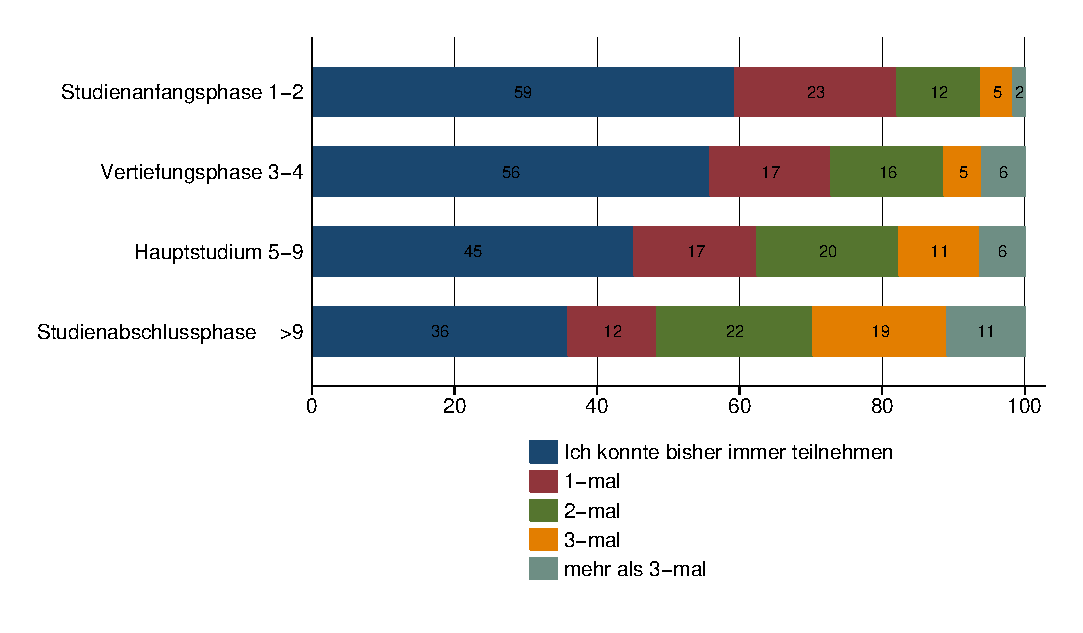
\includegraphics[
%  defaultresolution=72 !,
%  bmpsizefast=false
%]{image}
%\end{verbatim}
% \end{quote}
%
% \subsubsection{Hints}
%
% \begin{itemize}
% \item My version of \xfile{dvips.def} 1999/02/16 v3.0i defines
%       rules for the supported bitmap extensions, but does not
%       include them in the list of extensions that are tried
%       if the file name is not given with an extension.
%       In such a case, the list of extensions can be set
%       by \cs{DeclareGraphicsExtensions}, see \xpackage{grfguide}.
%       The following code just extends the list:
%       \begin{quote}
%\begin{verbatim}
%\makeatletter
%\g@addto@macro\Gin@extensions{,.bmp,.pcx,.msp}
%\makeatother
%\end{verbatim}
%       \end{quote}
% \item My version of \xfile{dvipdfm.def} 1998/11/24 vx.x misses
%       the graphics rule for PNG files. It can be added by:
%       \begin{quote}
%\begin{verbatim}
%\DeclareGraphicsRule{.png}{bmp}{.bb}{#1}
%\end{verbatim}
%       \end{quote}
%       See the previous issue to add the extension \xfile{.png} to the list
%       of extensions for package \xpackage{graphics}.
% \end{itemize}
%
% \subsubsection{Test program}
%
% There is a test program \xfile{bmpsize-test.tex}. Run it through
% \verb|latex|, \verb|pdflatex|, or \verb|pdftex|. Then given
% image files are inspected and the result is printed.
%
% \subsubsection{Interface for programmers}
%
% The macro names of the parsers are \verb|\bmpsize@read@|\meta{type}.
% Example: \cs{bmpsize@read@jpg} in case of JPEG.
%
% A parser sets the switch \cs{ifbmpsize@ok} to true, if it
% could successfully parse the image file.
% The width and height are returnd in \cs{bmpsize@width} and
% \cs{bmpsize@height}. If information about density is available,
% it is used to calculate width and height of the image, otherwise
% the values given by option \xoption{defaultresolution} is used.
% \xoption{resolution} overwrites the values in the image file.
%
% \subsection{Improved bitmap inclusion}
%
% Some drivers for package \xpackage{graphics} define the graphics
% type \xoption{bmp} for bitmap images. The code in the standard
% drivers for \xoption{dvips}, \xoption{dvipdfm}, and \xoption{dvipdfmx}
% is very basic and misses essential features of the
% package \xpackage{graphicx}. Therefore the code for bitmap
% inclusion is automatically rewritten by this package to add
% the following features:
% \begin{itemize}
% \item Support for \xoption{viewport} and \xoption{trim}.
% \item Support for \xoption{clip}.
% \item In case of \xoption{dvipdfm} and \xoption{dvipdfmx} the
%       bitmap images are reused and not included again if they
%       are used more than once.
% \end{itemize}
% However, there is a difference between \xoption{dvipdfm} and
% \xoption{dvipdfmx}, especially if images are reused. In the
% former case the reused box has width and height of 1bp, in the
% latter case its natural width. Thus the correct driver option must be given.
% \xoption{dvipdfm} and \xoption{dvipdfmx} are not equivalent.
%
% Older versions of \xoption{dvipdfmx} uses a size of 1in. However I do
% want to distinguish between versions of the same program. Therefore the
% support of these older versions has stopped with version 1.6 of this package.
% Use version dvipdfmx-20090708 or newer (some few versions before will
% probably also work, but I don't want to investigate this further).
%
% \StopEventually{
% }
%
% \section{Implementation}
%
% \subsection{Basic package \xpackage{bmpsize-base}}
%
%    Identification.
%    \begin{macrocode}
%<*base>
\ProvidesPackage{bmpsize-base}%
  [2009/09/04 v1.6 Basic part of bmpsize (HO)]%
%    \end{macrocode}
%    Modules of package \xpackage{fp} are used for calculations.
%    \begin{macrocode}
\RequirePackage{fp-basic}
\RequirePackage{fp-snap}
%    \end{macrocode}
%    Package \xpackage{fp} uses nested \cs{loop} structures.
%    That breaks with the plain-\TeX\ version of \cs{loop}.
%    Therefore we use the \LaTeX\ variant.
%    \begin{macro}{\@bmpsize@plain@loop}
%    \begin{macrocode}
\long\def\@bmpsize@plain@loop#1\repeat{%
  \def\iterate{%
    #1\relax
    \expandafter\iterate\fi
  }%
  \iterate
  \let\iterate\relax
}
%    \end{macrocode}
%    \end{macro}
%    \begin{macrocode}
\RequirePackage{pdftexcmds}[2007/11/11]
%    \end{macrocode}
%    \begin{macrocode}
\newif\ifbmpsize@ok
\let\@bmpsize@ok\bmpsize@oktrue

\newif\if@bmpsize@bigendian
\newif\if@bmpsize@absnum
\newif\if@bmpsize@user@resolution
\newif\if@bmpsize@fast
\@bmpsize@fasttrue

\def\@bmpsize@init{%
  \let\@bmpsize@org@plain@loop\loop
  \let\loop\@bmpsize@plain@loop
  \bmpsize@okfalse
  \@bmpsize@bigendiantrue
  \@bmpsize@absnumfalse
  \let\bmpsize@pixelwidth\relax
  \let\bmpsize@pixelheight\relax
  \let\bmpsize@pixelx\relax
  \let\bmpsize@pixely\relax
  \let\bmpsize@unit\relax
  \let\bmpsize@pixelxdenom\relax
  \let\bmpsize@pixelydenom\relax
  \let\bmpsize@orientation\relax
}

\def\@bmpsize@stop#1\@nil{}

\def\@bmpsize@loop#1{%
  #1%
  \@bmpsize@loop{#1}%
}
\def\@bmpsize@break#1\@bmpsize@loop#2{}

\def\@bmpsize@size#1#2#3{%
  \edef#3{\pdf@filesize{#1}}%
  \ifx#3\@empty
    \expandafter\@bmpsize@stop
  \fi
  \ifnum#3<#2\relax
    \expandafter\@bmpsize@stop
  \fi
}

\def\@bmpsize@read#1#2#3{%
  \edef\@bmpsize@buf{\pdf@filedump{#3}{#2}{#1}}%
  \edef\@bmpsize@temp{%
    \noexpand\@bmpsize@check@byte{#2}\@bmpsize@buf{}{}\noexpand\\%
  }%
  \@bmpsize@temp
}
\def\@bmpsize@fillbuf#1{%
  \ifx\@bmpsize@buf\@empty
    \expandafter\@firstofone
  \else
    \expandafter\@gobble
  \fi
  {%
    \edef\@bmpsize@buf{%
      \pdf@filedump{\bmpsize@offset}{\bmpsize@fillbuflength}{#1}%
    }%
    \ifx\@bmpsize@buf\@empty
      \expandafter\@bmpsize@stop
    \fi
    \edef\bmpsize@offset{\the\numexpr\bmpsize@offset+\bmpsize@fillbuflength}%
  }%
}
\def\bmpsize@fillbuflength{10}

\def\@bmpsize@append#1#2#3{%
  \edef#1{#2#3}%
}
\def\@bmpsize@pushback#1{%
  \edef\@bmpsize@buf{#1\@bmpsize@buf}%
}

\def\@bmpsize@iswhite#1{%
  \ifnum\pdf@strcmp{#1}{09}=\z@
  \else
    \ifnum\pdf@strcmp{#1}{0A}=\z@
    \else
      \ifnum\pdf@strcmp{#1}{0D}=\z@
      \else
        \ifnum\pdf@strcmp{#1}{20}=\z@
        \else
          1%
        \fi
      \fi
    \fi
  \fi
  \space
}
\def\@bmpsize@isdigit#1{%
  \ifnum\pdf@strcmp{#1}{30}<\z@
    1%
  \else
    \ifnum\pdf@strcmp{#1}{39}>\z@
      1%
    \fi
  \fi
  \space
}

\def\@bmpsize@check@byte#1#2#3{%
  \ifnum#1<\@ne
    \csname fi\endcsname
    \@bmpsize@cleanup@end
  \else
    \csname fi\endcsname
  \ifx!#2#3!%
    \csname fi\endcsname
    \@bmpsize@stop
  \else
    \csname fi\endcsname
    \expandafter\@bmpsize@check@byte\expandafter{\the\numexpr#1-1}%
}
\def\@bmpsize@cleanup@end#1\\{}

\def\@bmpsize@swap@maybe#1{%
  \if@bmpsize@bigendian
  \else
    \edef#1{\expandafter\@bmpsize@@swap#1\@empty\@empty\@empty\@empty}%
  \fi
}
\def\@bmpsize@@swap#1#2#3#4#5#6#7#8{%
  #7#8#5#6#3#4#1#2%
}

\def\@bmpsize@skip@one{%
  \edef\@bmpsize@buf{\expandafter\@gobbletwo\@bmpsize@buf}%
}
\def\@bmpsize@skip@two{%
  \edef\@bmpsize@buf{\expandafter\@gobblefour\@bmpsize@buf}%
}
\def\@bmpsize@skip@four{%
  \edef\@bmpsize@buf{%
    \expandafter\expandafter\expandafter\@gobblefour\expandafter
    \@gobblefour\@bmpsize@buf
  }%
}

\def\@bmpsize@grab#1#2{%
  \edef#1{\noexpand\@bmpsize@grab@byte#2=\@bmpsize@buf\noexpand\\}%
  \edef#1{#1}%
}
\def\@bmpsize@grab@byte#1=#2#3{%
  #2#3%
  \ifnum#1>\@ne
    \expandafter\@bmpsize@grab@byte\the\numexpr#1-1\expandafter=%
  \else
    \expandafter\@bmpsize@cleanup@end
  \fi
}

\def\@bmpsize@abs@maybe#1{%
  \let\@bmpsize@temp\relax
  \if@bmpsize@absnum
    \ifnum"\expandafter\@car#1\@nil>7 %
      \edef#1{\expandafter\@bmpsize@abs@byte#1\relax}%
      \ifnum\pdf@strcmp{#1}{7FFFFFFF}=\z@
        \let\@bmpsize@temp\@bmpsize@stop
      \else
        \def\@bmpsize@temp{\edef#1{\the\numexpr#1+1}}%
      \fi
    \fi
  \fi
}
\def\@bmpsize@abs@byte#1{%
  \ifx#1\relax
  \else
    \ifcase"0#1 %
      F\or E\or D\or C\or B\or A\or 9\or 8\or
      7\or 6\or 5\or 4\or 3\or 2\or 1\or 0%
    \fi
    \expandafter\@bmpsize@abs@byte
  \fi
}

\def\@bmpsize@num@one#1{%
  \@bmpsize@grab#11%
  \@bmpsize@abs@maybe#1%
  \edef#1{\number"#1}%
  \@bmpsize@temp
  \@bmpsize@skip@one
}
\def\@bmpsize@num@two#1{%
  \@bmpsize@grab#12%
  \@bmpsize@swap@maybe#1%
  \@bmpsize@abs@maybe#1%
  \edef#1{\number"#1}%
  \@bmpsize@temp
  \@bmpsize@skip@two
}
\def\@bmpsize@num@four#1{%
  \@bmpsize@grab#14%
  \@bmpsize@swap@maybe#1%
  \@bmpsize@abs@maybe#1%
  \ifnum\pdf@strcmp{#1}{7FFFFFFF}>\z@
    \expandafter\@bmpsize@stop
  \fi
  \edef#1{\number"#1}%
  \@bmpsize@temp
  \@bmpsize@skip@four
}

\def\@bmpsize@div#1#2#3{% #1 := #2/#3
  \FPdiv#1{#2}{#3}%
  \@bmpsize@beautify#1%
}
\def\@bmpsize@beautify#1{%
  \FPifint#1%
    \edef#1{\expandafter\@bmpsize@trunc#1.\@nil}%
  \else
    \edef#1{\expandafter\@bmpsize@cleanup@frac#1.\@nil}%
  \fi
}
\def\@bmpsize@trunc#1.#2\@nil{#1}
% #1 isn't an integer, thus we should have at least one
% necessary digit after the dot
\def\@bmpsize@cleanup@frac#1.#2#3.#4\@nil{%
  #1.#2%
  \ifx\\#3\\%
  \else
    \@bmpsize@cleanup@fracdigits#3000000000\@nil
  \fi
}
\def\@bmpsize@cleanup@fracdigits#1#2#3#4#5#6#7#8#9{%
  \ifcase#9 %
    \ifcase#8 %
      \ifcase#7 %
        \ifcase#6 %
          \ifcase#5 %
            \ifcase #4 %
              \ifcase #3 %
                \ifcase #2 %
                  \ifcase #1 %
                  \else
                    #1%
                  \fi
                \else
                  #1#2%
                \fi
              \else
                #1#2#3%
              \fi
            \else
              #1#2#3#4%
            \fi
          \else
            #1#2#3#4#5%
          \fi
        \else
          #1#2#3#4#5#6%
        \fi
      \else
        #1#2#3#4#5#6#7%
      \fi
    \else
      #1#2#3#4#5#6#7#8%
    \fi
  \else
    #1#2#3#4#5#6#7#8#9%
  \fi
  \@bmpsize@trunc.%
}

\def\@bmpsize@end{%
  \ifbmpsize@ok
    \ifx\bmpsize@pixelwidth\relax
      \bmpsize@okfalse
    \fi
    \ifx\bmpsize@pixelheight\relax
      \bmpsize@okfalse
    \fi
  \fi
  \ifbmpsize@ok
    \ifnum\bmpsize@pixelwidth>\z@
    \else
      \bmpsize@okfalse
    \fi
    \ifnum\bmpsize@pixelheight>\z@
    \else
      \bmpsize@okfalse
    \fi
  \fi
  \ifbmpsize@ok
    \ifcase 0%
      \ifx\bmpsize@pixelx\relax 1 \fi
      \ifx\bmpsize@pixely\relax 1 \fi
      \ifnum\bmpsize@pixelx>\z@\else 1 \fi
      \ifnum\bmpsize@pixely>\z@\else 1 \fi
      \ifx\bmpsize@pixelxdenom\relax
         \ifx\bmpsize@pixelydenom\relax\else 1 \fi
      \else
        \ifnum\bmpsize@pixelxdenom>\z@\else 1 \fi
      \fi
      \ifx\bmpsize@pixelydenom\relax
      \else
        \ifnum\bmpsize@pixelydenom>\z@\else 1 \fi
      \fi
    \else
      \let\bmpsize@pixelx\relax
      \let\bmpsize@pixely\relax
      \let\bmpsize@unit\relax
      \let\bmpsize@pixelxdenom\relax
      \let\bmpsize@pixelydenom\relax
    \fi
    \ifx\bmpsize@pixelxdenom\relax
    \else
      \@bmpsize@div\bmpsize@pixelx\bmpsize@pixelx\bmpsize@pixelxdenom
      \@bmpsize@div\bmpsize@pixely\bmpsize@pixely\bmpsize@pixelydenom
      \let\bmpsize@pixelxdenom\relax
      \let\bmpsize@pixelydenom\relax
    \fi
    \ifcase 0\ifx\bmpsize@unit\relax 1\fi
             \if@bmpsize@user@resolution 1\fi
             \relax
      \let\bmpsize@calc@unit\bmpsize@unit
      \let\bmpsize@calc@pixelx\bmpsize@pixelx
      \let\bmpsize@calc@pixely\bmpsize@pixely
    \else
      \let\bmpsize@calc@unit\bmpsize@unit@default
      \let\bmpsize@calc@pixelx\bmpsize@pixelx@default
      \let\bmpsize@calc@pixely\bmpsize@pixely@default
      \ifx\bmpsize@calc@pixely\Gin@exclamation
        \ifx\bmpsize@pixelx\relax
          \let\bmpsize@calc@pixely\bmpsize@calc@pixelx
        \else
          \FPdiv\bmpsize@calc@pixely\bmpsize@calc@pixelx\bmpsize@pixelx
          \FPmul\bmpsize@calc@pixely\bmpsize@calc@pixely\bmpsize@pixely
        \fi
      \else
        \ifx\bmpsize@calc@pixelx\Gin@exclamation
          \ifx\bmpsize@pixelx\relax
            \let\bmpsize@calc@pixelx\bmpsize@calc@pixely
          \else
            \FPdiv\bmpsize@calc@pixelx\bmpsize@calc@pixely\bmpsize@pixely
            \FPmul\bmpsize@calc@pixelx\bmpsize@calc@pixelx\bmpsize@pixelx
          \fi
        \fi
      \fi
    \fi
    \FPdiv\bmpsize@width\bmpsize@pixelwidth\bmpsize@calc@pixelx
    \FPdiv\bmpsize@height\bmpsize@pixelheight\bmpsize@calc@pixely
    % calculation of width and height in bp for package graphics
    % 1in = 72bp = 72.27pt, 72/72.27 = 8/8.03, 1pt = 65536sp
    \if@bmpsize@fast
      \edef\bmpsize@width{%
        \strip@pt\dimexpr.99626\dimexpr
        \bmpsize@width\dimexpr\bmpsize@calc@unit
      }%
      \edef\bmpsize@height{%
        \strip@pt\dimexpr.99626\dimexpr
        \bmpsize@height\dimexpr\bmpsize@calc@unit
      }%
    \else
      \edef\@bmpsize@temp{\number\dimexpr\bmpsize@calc@unit}%
      \ifnum\@bmpsize@temp>100000 %
        \FPmul\@bmpsize@temp\@bmpsize@temp{0.00001}%
        \def\@bmpsize@corr{100000}%
      \else
        \let\@bmpsize@corr\relax
      \fi
      \FPmul\bmpsize@width\bmpsize@width\@bmpsize@temp
      \FPmul\bmpsize@height\bmpsize@height\@bmpsize@temp
      \FPmul\bmpsize@width\bmpsize@width{8}%
      \FPmul\bmpsize@height\bmpsize@height{8}%
      \FPdiv\bmpsize@width\bmpsize@width{8.03}%
      \FPdiv\bmpsize@height\bmpsize@height{8.03}%
      \FPdiv\bmpsize@width\bmpsize@width{65536}%
      \FPdiv\bmpsize@height\bmpsize@height{65536}%
      \ifx\@bmpsize@corr\relax
      \else
        \FPmul\bmpsize@width\bmpsize@width\@bmpsize@corr
        \FPmul\bmpsize@height\bmpsize@height\@bmpsize@corr
      \fi
      \FPround\bmpsize@width\bmpsize@width{5}%
      \FPround\bmpsize@height\bmpsize@height{5}%
      \@bmpsize@beautify\bmpsize@width
      \@bmpsize@beautify\bmpsize@height
    \fi
  \fi
  \let\loop\@bmpsize@org@plain@loop
}
\def\bmpsize@unit@default{72.27pt}% more accurate than 1in
\def\bmpsize@pixelx@default{72}
\let\bmpsize@pixely@default\Gin@exclamation

\def\bmpsize@types{png,jpg,bmp,gif,tiff,pnm,pam,xpm,tga,pcx,msp,sgi}
%</base>
%    \end{macrocode}
%
% \subsection{Bitmap formats}
%
% \subsubsection{png}
%
%\iffalse
%<*ignore>
%\fi
%\begin{verbatim}
%begin png
%big-endian
%
%read 24 0
%grab 8        -> $temp
%check streq $temp [0x89 "PNG" 0x0D 0x0A 0x1A 0x0A]
%num 4         -> $length
%grab 4        -> $temp
%check streq $temp ["IHDR"]
%num 4         -> $pixelwidth
%num 4         -> $pixelheight
%ok
%assign numexpr(20 + $length) -> $offset
%loop
%  read 8 $offset
%  num 4       -> $length
%  grab 4      -> $temp
%  if streq $temp ["IDAT"]
%    stop
%  fi
%  if streq $temp ["pHYs"]
%    read 9 numexpr($offset + 8)
%    num 4     -> $pixelx
%    num 4     -> $pixely
%    grab 1     -> $temp
%    if numeq $temp 1
%      assign {100cm} -> $unit
%    fi
%    stop
%  fi
%  assign numexpr($offset + 12 + $length) -> $offset
%repeat
%end
%\end{verbatim}
%\iffalse
%</ignore>
%\fi
%    \begin{macro}{\bmpsize@read@png}
%    \begin{macrocode}
%<*base>
\def\bmpsize@read@png#1{%
  \@bmpsize@init
  \@bmpsize@bigendiantrue
  \@bmpsize@read{#1}{24}{0}%
  \@bmpsize@grab\bmpsize@temp{8}%
  \@bmpsize@skip@four
  \@bmpsize@skip@four
  \ifnum\pdf@strcmp{\bmpsize@temp}{89504E470D0A1A0A}=\z@
  \else
    \expandafter\@bmpsize@stop
  \fi
  \@bmpsize@num@four\bmpsize@length
  \@bmpsize@grab\bmpsize@temp{4}%
  \@bmpsize@skip@four
  \ifnum\pdf@strcmp{\bmpsize@temp}{49484452}=\z@
  \else
    \expandafter\@bmpsize@stop
  \fi
  \@bmpsize@num@four\bmpsize@pixelwidth
  \@bmpsize@num@four\bmpsize@pixelheight
  \@bmpsize@ok
  \edef\bmpsize@offset{\the\numexpr20+\bmpsize@length}%
  \@bmpsize@loop{%
    \@bmpsize@read{#1}{8}{\bmpsize@offset}%
    \@bmpsize@num@four\bmpsize@length
    \@bmpsize@grab\bmpsize@temp{4}%
    \@bmpsize@skip@four
    \ifnum\pdf@strcmp{\bmpsize@temp}{49444154}=\z@
      \expandafter\@firstofone
    \else
      \expandafter\@gobble
    \fi
    {%
      \@bmpsize@stop
    }%
    \ifnum\pdf@strcmp{\bmpsize@temp}{70485973}=\z@
      \expandafter\@firstofone
    \else
      \expandafter\@gobble
    \fi
    {%
      \@bmpsize@read{#1}{9}{\numexpr\bmpsize@offset+8\relax}%
      \@bmpsize@num@four\bmpsize@pixelx
      \@bmpsize@num@four\bmpsize@pixely
      \@bmpsize@grab\bmpsize@temp{1}%
      \@bmpsize@skip@one
      \ifnum\bmpsize@temp=1\relax
        \expandafter\@firstofone
      \else
        \expandafter\@gobble
      \fi
      {%
        \def\bmpsize@unit{100cm}%
      }%
      \@bmpsize@stop
    }%
    \edef\bmpsize@offset{\the\numexpr\bmpsize@offset+12+\bmpsize@length}%
  }%
  \@bmpsize@stop
  \@nil
  \@bmpsize@end
}%
%</base>
%    \end{macrocode}
%    \end{macro}
%
% \subsubsection{jpg}
%
%\iffalse
%<*ignore>
%\fi
%\begin{verbatim}
%begin jpg
%
%read 3 0
%grab 3      -> $temp % SOI and 0xFF
%check streq $temp [0xFF 0xD8 0xFF]
%assign {2} -> $offset
%assign {0} -> $exifdensity
%loop
%  read 4 $offset
%  grab 1    -> $temp
%  check streq $temp [0xFF]
%  num 1    -> $temp
%  if numeq $temp 0xDA % SOS
%    stop
%  fi
%  % look for JFIF APP0 segment
%  if numeq $temp 0xE0 % APP0
%    num 2       -> $length
%    if numeq $exifdensity 0
%      if numge $length 16 % a JFIF segment has 16 bytes at least
%        read 12 numexpr($offset + 4)
%        grab 5      -> $temp % identifier
%        if streq $temp ["JFIF" 0x0]
%          check numge $length 16
%          skip 2 % version
%          num 1       -> $temp % units
%          if numeq $temp 1
%            assign {72.27pt} -> $unit
%          else
%            if numeq $temp 2
%              assign {1cm} -> $unit
%            fi
%          fi
%          num 2    -> $pixelx
%          num 2    -> $pixely
%        fi
%      fi
%    fi
%  else
%    if numeq $temp 0xE1 % APP1
%      % look for Exif APP1 segment
%      num 2 -> $length
%      if numge $length 20 % identifier (6) + Tiff header (8) + first IFD (>=6)
%        read 20 numexpr($offset + 4)
%        grab 6 -> $temp
%        if streq $temp ["Exif" 0x0 0x0]
%          assign numexpr($offset + 10) -> $exifoffset
%          % read TIFF header
%          grab 2 -> $temp
%          if streq $temp ["II"]
%            little-endian
%          else
%            check streq $temp ["MM"]
%            % big-endian
%          fi
%          num 2 -> $temp
%          check numeq $temp 42
%          num 4 -> $temp % offset of first IFD
%          check numgt $temp 0
%          % read first IFD
%          assign numexpr($temp + $exifoffset) -> $off
%          read 2 $off
%          num 2 -> $entries
%          assign numexpr($off + 2) -> $off
%          loop
%            if numeq $entries 0
%              break
%            fi
%            assign numexpr($entries - 1) -> $entries
%            % entry format:
%            % 2 tag
%            % 2 field type
%            % 4 count
%            % 4 value/offset
%            read 12 $off
%            assign numexpr($off + 12) -> $off
%            num 2 -> $tag
%            if numeq $tag 296 % ResolutionUnit
%              skip 6 % type: 3 (short), count: 1
%              num 2 -> $temp
%              ifcase $temp
%              or % 1
%                clear $unit
%              or % 2
%                assign {72.27pt} -> $unit
%              or % 3
%                assign {1cm} -> $unit
%              else
%                clear $unit % unknown
%              fi
%              ifcase $temp
%              or % 1
%              or % 2
%                assign {1} -> $exifdensity
%              or % 3
%                assign {1} -> $exifdensity
%              else
%                assign $exifdensity -> $exifdensity
%              fi
%            fi
%            % 256 ImageWidth (use width of JPG part)
%            % 257 ImageHeight (use height of JPG part)
%            if numeq $tag 274 % Orientation
%              skip 6 % type: 3 (short), count: 1
%              num 2 -> $temp
%              if numge $temp 0 
%                if numle $temp 8
%                  assign $temp -> $orientation
%                fi
%              fi
%            fi
%            if numeq $tag 282 % XResolution
%              skip 6
%              num 4 -> $temp
%              read 8 numexpr($temp + $exifoffset)
%              num 4 -> $pixelx
%              num 4 -> $temp
%              if numeq $temp 1
%              else
%                assign numexpr($temp) -> $pixelxdenom
%                % div $pixelx $temp -> $pixelx
%              fi
%            fi
%            if numeq $tag 283 % YResolution
%              skip 6
%              num 4 -> $temp
%              read 8 numexpr($temp + $exifoffset)
%              num 4 -> $pixely
%              num 4 -> $temp
%              if numeq $temp 1
%              else
%                assign numexpr($temp) -> $pixelydenom
%                % div $pixely $temp -> $pixely
%              fi
%            fi
%          repeat
%          big-endian
%        fi
%      fi
%    else
%      assign numexpr($temp - 0xC0) -> $temp
%      ifcase $temp % SOF_0
%      or % SOF_1
%      or % SOF_2
%      or % SOF_3
%      or % DHT
%        assign {-1} -> $temp
%      or % SOF_5
%      or % SOF_6
%      or % SOF_7
%      or % JPG
%        assign {-1} -> $temp
%      or % SOF_9
%      or % SOF_10
%      or % SOF_11
%      or % DAC
%        assign {-1} -> $temp
%      or % SOF_13
%      or % SOF_14
%      or % SOF_15
%      else
%        assign {-1} -> $temp
%      fi
%      if numeq $temp -1
%      else
%        read 4 numexpr($offset + 5)
%        num 2  -> $pixelheight
%        num 2  -> $pixelwidth
%        if numeq $pixelheight 0
%          clear $pixelheight
%          stop
%        fi
%        ok
%        stop
%      fi
%      num 2 -> $length
%    fi
%  fi
%  assign numexpr($offset + $length + 2) -> $offset
%repeat
%end
%\end{verbatim}
%\iffalse
%</ignore>
%\fi
%    \begin{macro}{\bmpsize@read@jpg}
%    \begin{macrocode}
%<*base>
\def\bmpsize@read@jpg#1{%
  \@bmpsize@init
  \@bmpsize@read{#1}{3}{0}%
  \@bmpsize@grab\bmpsize@temp{3}%
  \@bmpsize@skip@two
  \@bmpsize@skip@one
  \ifnum\pdf@strcmp{\bmpsize@temp}{FFD8FF}=\z@
  \else
    \expandafter\@bmpsize@stop
  \fi
  \def\bmpsize@offset{2}%
  \def\bmpsize@exifdensity{0}%
  \@bmpsize@loop{%
    \@bmpsize@read{#1}{4}{\bmpsize@offset}%
    \@bmpsize@grab\bmpsize@temp{1}%
    \@bmpsize@skip@one
    \ifnum\pdf@strcmp{\bmpsize@temp}{FF}=\z@
    \else
      \expandafter\@bmpsize@stop
    \fi
    \@bmpsize@num@one\bmpsize@temp
    \ifnum\bmpsize@temp=218\relax
      \expandafter\@firstofone
    \else
      \expandafter\@gobble
    \fi
    {%
      \@bmpsize@stop
    }%
    \ifnum\bmpsize@temp=224\relax
      \expandafter\@firstoftwo
    \else
      \expandafter\@secondoftwo
    \fi
    {%
      \@bmpsize@num@two\bmpsize@length
      \ifnum\bmpsize@exifdensity=0\relax
        \expandafter\@firstofone
      \else
        \expandafter\@gobble
      \fi
      {%
        \unless\ifnum\bmpsize@length<16\relax
          \expandafter\@firstofone
        \else
          \expandafter\@gobble
        \fi
        {%
          \@bmpsize@read{#1}{12}{\numexpr\bmpsize@offset+4\relax}%
          \@bmpsize@grab\bmpsize@temp{5}%
          \@bmpsize@skip@four
          \@bmpsize@skip@one
          \ifnum\pdf@strcmp{\bmpsize@temp}{4A46494600}=\z@
            \expandafter\@firstofone
          \else
            \expandafter\@gobble
          \fi
          {%
            \ifnum\bmpsize@length<16\relax
              \expandafter\@bmpsize@stop
            \fi
            \@bmpsize@skip@two
            \@bmpsize@num@one\bmpsize@temp
            \ifnum\bmpsize@temp=1\relax
              \expandafter\@firstoftwo
            \else
              \expandafter\@secondoftwo
            \fi
            {%
              \def\bmpsize@unit{72.27pt}%
            }{%
              \ifnum\bmpsize@temp=2\relax
                \expandafter\@firstofone
              \else
                \expandafter\@gobble
              \fi
              {%
                \def\bmpsize@unit{1cm}%
              }%
            }%
            \@bmpsize@num@two\bmpsize@pixelx
            \@bmpsize@num@two\bmpsize@pixely
          }%
        }%
      }%
    }{%
      \ifnum\bmpsize@temp=225\relax
        \expandafter\@firstoftwo
      \else
        \expandafter\@secondoftwo
      \fi
      {%
        \@bmpsize@num@two\bmpsize@length
        \unless\ifnum\bmpsize@length<20\relax
          \expandafter\@firstofone
        \else
          \expandafter\@gobble
        \fi
        {%
          \@bmpsize@read{#1}{20}{\numexpr\bmpsize@offset+4\relax}%
          \@bmpsize@grab\bmpsize@temp{6}%
          \@bmpsize@skip@four
          \@bmpsize@skip@two
          \ifnum\pdf@strcmp{\bmpsize@temp}{457869660000}=\z@
            \expandafter\@firstofone
          \else
            \expandafter\@gobble
          \fi
          {%
            \edef\bmpsize@exifoffset{\the\numexpr\bmpsize@offset+10}%
            \@bmpsize@grab\bmpsize@temp{2}%
            \@bmpsize@skip@two
            \ifnum\pdf@strcmp{\bmpsize@temp}{4949}=\z@
              \expandafter\@firstoftwo
            \else
              \expandafter\@secondoftwo
            \fi
            {%
              \@bmpsize@bigendianfalse
            }{%
              \ifnum\pdf@strcmp{\bmpsize@temp}{4D4D}=\z@
              \else
                \expandafter\@bmpsize@stop
              \fi
            }%
            \@bmpsize@num@two\bmpsize@temp
            \ifnum\bmpsize@temp=42\relax
            \else
              \expandafter\@bmpsize@stop
            \fi
            \@bmpsize@num@four\bmpsize@temp
            \ifnum\bmpsize@temp>0\relax
            \else
              \expandafter\@bmpsize@stop
            \fi
            \edef\bmpsize@off{\the\numexpr\bmpsize@temp+\bmpsize@exifoffset}%
            \@bmpsize@read{#1}{2}{\bmpsize@off}%
            \@bmpsize@num@two\bmpsize@entries
            \edef\bmpsize@off{\the\numexpr\bmpsize@off+2}%
            \@bmpsize@loop{%
              \ifnum\bmpsize@entries=0\relax
                \expandafter\@firstofone
              \else
                \expandafter\@gobble
              \fi
              {%
                \@bmpsize@break
              }%
              \edef\bmpsize@entries{\the\numexpr\bmpsize@entries-1}%
              \@bmpsize@read{#1}{12}{\bmpsize@off}%
              \edef\bmpsize@off{\the\numexpr\bmpsize@off+12}%
              \@bmpsize@num@two\bmpsize@tag
              \ifnum\bmpsize@tag=296\relax
                \expandafter\@firstofone
              \else
                \expandafter\@gobble
              \fi
              {%
                \@bmpsize@skip@four
                \@bmpsize@skip@two
                \@bmpsize@num@two\bmpsize@temp
                \ifcase\bmpsize@temp\relax
                \or
                  \let\bmpsize@unit\relax
                \or
                  \def\bmpsize@unit{72.27pt}%
                \or
                  \def\bmpsize@unit{1cm}%
                \else
                  \let\bmpsize@unit\relax
                \fi
                \ifcase\bmpsize@temp\relax
                \or
                \or
                  \def\bmpsize@exifdensity{1}%
                \or
                  \def\bmpsize@exifdensity{1}%
                \else
                  \let\bmpsize@exifdensity\bmpsize@exifdensity
                \fi
              }%
              \ifnum\bmpsize@tag=274\relax
                \expandafter\@firstofone
              \else
                \expandafter\@gobble
              \fi
              {%
                \@bmpsize@skip@four
                \@bmpsize@skip@two
                \@bmpsize@num@two\bmpsize@temp
                \unless\ifnum\bmpsize@temp<0\relax
                  \expandafter\@firstofone
                \else
                  \expandafter\@gobble
                \fi
                {%
                  \unless\ifnum\bmpsize@temp>8\relax
                    \expandafter\@firstofone
                  \else
                    \expandafter\@gobble
                  \fi
                  {%
                    \let\bmpsize@orientation\bmpsize@temp
                  }%
                }%
              }%
              \ifnum\bmpsize@tag=282\relax
                \expandafter\@firstofone
              \else
                \expandafter\@gobble
              \fi
              {%
                \@bmpsize@skip@four
                \@bmpsize@skip@two
                \@bmpsize@num@four\bmpsize@temp
                \@bmpsize@read{#1}{8}{\numexpr\bmpsize@temp+\bmpsize@exifoffset\relax}%
                \@bmpsize@num@four\bmpsize@pixelx
                \@bmpsize@num@four\bmpsize@temp
                \ifnum\bmpsize@temp=1\relax
                  \expandafter\@gobble
                \else
                  \expandafter\@firstofone
                \fi
                {%
                  \edef\bmpsize@pixelxdenom{\the\numexpr\bmpsize@temp}%
                }%
              }%
              \ifnum\bmpsize@tag=283\relax
                \expandafter\@firstofone
              \else
                \expandafter\@gobble
              \fi
              {%
                \@bmpsize@skip@four
                \@bmpsize@skip@two
                \@bmpsize@num@four\bmpsize@temp
                \@bmpsize@read{#1}{8}{\numexpr\bmpsize@temp+\bmpsize@exifoffset\relax}%
                \@bmpsize@num@four\bmpsize@pixely
                \@bmpsize@num@four\bmpsize@temp
                \ifnum\bmpsize@temp=1\relax
                  \expandafter\@gobble
                \else
                  \expandafter\@firstofone
                \fi
                {%
                  \edef\bmpsize@pixelydenom{\the\numexpr\bmpsize@temp}%
                }%
              }%
            }%
            \@bmpsize@bigendiantrue
          }%
        }%
      }{%
        \edef\bmpsize@temp{\the\numexpr\bmpsize@temp-192}%
        \ifcase\bmpsize@temp\relax
        \or
        \or
        \or
        \or
          \def\bmpsize@temp{-1}%
        \or
        \or
        \or
        \or
          \def\bmpsize@temp{-1}%
        \or
        \or
        \or
        \or
          \def\bmpsize@temp{-1}%
        \or
        \or
        \or
        \else
          \def\bmpsize@temp{-1}%
        \fi
        \ifnum\bmpsize@temp=-1\relax
          \expandafter\@gobble
        \else
          \expandafter\@firstofone
        \fi
        {%
          \@bmpsize@read{#1}{4}{\numexpr\bmpsize@offset+5\relax}%
          \@bmpsize@num@two\bmpsize@pixelheight
          \@bmpsize@num@two\bmpsize@pixelwidth
          \ifnum\bmpsize@pixelheight=0\relax
            \expandafter\@firstofone
          \else
            \expandafter\@gobble
          \fi
          {%
            \let\bmpsize@pixelheight\relax
            \@bmpsize@stop
          }%
          \@bmpsize@ok
          \@bmpsize@stop
        }%
        \@bmpsize@num@two\bmpsize@length
      }%
    }%
    \edef\bmpsize@offset{\the\numexpr\bmpsize@offset+\bmpsize@length+2}%
  }%
  \@bmpsize@stop
  \@nil
  \@bmpsize@end
}%
%</base>
%    \end{macrocode}
%    \end{macro}
%
% \subsubsection{bmp}
%
%\iffalse
%<*ignore>
%\fi
%\begin{verbatim}
%begin bmp
%little-endian
%
%read 26 0
%grab 2 -> $temp
%check streq $temp ["BM"]
%skip 12
%% header size is 4 bytes in V3+, unknown for V1, V2,
%% known header sizes fit in 2 bytes
%num 2   -> $temp
%if numeq $temp 12 % V1
%  skip 2
%  num 2 -> $pixelwidth
%  num 2 -> $pixelheight
%  % no resolution entries
%  ok
%  stop
%fi
%if numeq $temp 64 % V2
%  skip 2
%  num 2 -> $pixelwidth
%  num 2 -> $pixelheight
%  % missing specification for resolution
%  ok
%  stop
%fi
%% V3, V4, V5
%skip 2
%num 4 -> $pixelwidth
%absnum 4 -> $pixelheight
%ok
%read 8 38
%num 4 -> $pixelx
%num 4 -> $pixely
%assign {100cm} -> $unit
%end
%\end{verbatim}
%\iffalse
%</ignore>
%\fi
%    \begin{macro}{\bmpsize@read@bmp}
%    \begin{macrocode}
%<*base>
\def\bmpsize@read@bmp#1{%
  \@bmpsize@init
  \@bmpsize@bigendianfalse
  \@bmpsize@read{#1}{26}{0}%
  \@bmpsize@grab\bmpsize@temp{2}%
  \@bmpsize@skip@two
  \ifnum\pdf@strcmp{\bmpsize@temp}{424D}=\z@
  \else
    \expandafter\@bmpsize@stop
  \fi
  \@bmpsize@skip@four
  \@bmpsize@skip@four
  \@bmpsize@skip@four
  \@bmpsize@num@two\bmpsize@temp
  \ifnum\bmpsize@temp=12\relax
    \expandafter\@firstofone
  \else
    \expandafter\@gobble
  \fi
  {%
    \@bmpsize@skip@two
    \@bmpsize@num@two\bmpsize@pixelwidth
    \@bmpsize@num@two\bmpsize@pixelheight
    \@bmpsize@ok
    \@bmpsize@stop
  }%
  \ifnum\bmpsize@temp=64\relax
    \expandafter\@firstofone
  \else
    \expandafter\@gobble
  \fi
  {%
    \@bmpsize@skip@two
    \@bmpsize@num@two\bmpsize@pixelwidth
    \@bmpsize@num@two\bmpsize@pixelheight
    \@bmpsize@ok
    \@bmpsize@stop
  }%
  \@bmpsize@skip@two
  \@bmpsize@num@four\bmpsize@pixelwidth
  \@bmpsize@absnumtrue
  \@bmpsize@num@four\bmpsize@pixelheight
  \@bmpsize@absnumfalse
  \@bmpsize@ok
  \@bmpsize@read{#1}{8}{38}%
  \@bmpsize@num@four\bmpsize@pixelx
  \@bmpsize@num@four\bmpsize@pixely
  \def\bmpsize@unit{100cm}%
  \@bmpsize@stop
  \@nil
  \@bmpsize@end
}%
%</base>
%    \end{macrocode}
%    \end{macro}
%
% \subsubsection{gif}
%
%\iffalse
%<*ignore>
%\fi
%\begin{verbatim}
%begin gif
%little-endian
%
%% Header
%read 13 0
%grab 3      -> $temp
%check streq $temp ["GIF"]
%skip 3      % version
%
%% Logical Screen Descriptor
%num 2       -> $pixelwidth
%num 2       -> $pixelheight
%skip 2
%num 1       -> $temp % Pixel Aspect Ratio
%if numeq $temp 0
%else
%  assign numexpr($temp + 15) -> $pixelx
%  assign {64}     -> $pixely
%fi
%ok
%end
%\end{verbatim}
%\iffalse
%</ignore>
%\fi
%    \begin{macro}{\bmpsize@read@gif}
%    \begin{macrocode}
%<*base>
\def\bmpsize@read@gif#1{%
  \@bmpsize@init
  \@bmpsize@bigendianfalse
  \@bmpsize@read{#1}{13}{0}%
  \@bmpsize@grab\bmpsize@temp{3}%
  \@bmpsize@skip@two
  \@bmpsize@skip@one
  \ifnum\pdf@strcmp{\bmpsize@temp}{474946}=\z@
  \else
    \expandafter\@bmpsize@stop
  \fi
  \@bmpsize@skip@two
  \@bmpsize@skip@one
  \@bmpsize@num@two\bmpsize@pixelwidth
  \@bmpsize@num@two\bmpsize@pixelheight
  \@bmpsize@skip@two
  \@bmpsize@num@one\bmpsize@temp
  \ifnum\bmpsize@temp=0\relax
    \expandafter\@gobble
  \else
    \expandafter\@firstofone
  \fi
  {%
    \edef\bmpsize@pixelx{\the\numexpr\bmpsize@temp+15}%
    \def\bmpsize@pixely{64}%
  }%
  \@bmpsize@ok
  \@bmpsize@stop
  \@nil
  \@bmpsize@end
}%
%</base>
%    \end{macrocode}
%    \end{macro}
%
% \subsubsection{tiff}
%
%\iffalse
%<*ignore>
%\fi
%\begin{verbatim}
%begin tiff
%% defaults
%assign {72.27pt} -> $unit
%
%% Image File Header
%read 8 0
%grab 2 -> $temp
%if streq $temp ["II"]
%  little-endian
%else
%  check streq $temp ["MM"]
%  big-endian
%fi
%num 2 -> $temp
%check numeq $temp 42
%num 4 -> $offset % first IFD (Image File Directory)
%
%% First IFD
%read 2 $offset
%assign numexpr($offset + 2) -> $offset
%num 2 -> $entries
%ok % must rely on checks at the end
%loop
%  if numeq $entries 0
%    stop
%  fi
%  assign numexpr($entries - 1) -> $entries
%  % entry format:
%  % 2 tag
%  % 2 field type
%  % 4 count
%  % 4 value/offset
%  read 12 $offset
%  assign numexpr($offset + 12) -> $offset
%  num 2 -> $tag % tag
%  if numeq $temp 296 % ResolutionUnit
%    skip 6 % type: 3 (short), count: 1
%    num 2 -> $temp
%    ifcase $temp
%    or % 1
%      clear $unit
%    or % 2
%      assign {72.27pt} -> $unit
%    or % 3
%      assign {1cm} -> $unit
%    else
%      clear $unit
%    fi
%  fi
%  if numeq $tag 256 % ImageWidth
%    skip 6
%    num 4 -> $pixelwidth
%  fi
%  if numeq $tag 257 % ImageLength
%    skip 6
%    num 4 -> $pixelheight
%  fi
%  if numeq $tag 282 % XResolution
%    skip 6
%    num 4 -> $temp
%    read 8 $temp
%    num 4 -> $pixelx
%    num 4 -> $temp
%    if numeq $temp 1
%    else
%      assign numexpr($temp) -> $pixelxdenom
%      % div $pixelx $temp -> $pixelx
%    fi
%  fi
%  if numeq $tag 283 % YResolution
%    skip 6
%    num 4 -> $temp
%    read 8 $temp
%    num 4 -> $pixely
%    num 4 -> $temp
%    if numeq $temp 1
%    else
%      assign numexpr($temp) -> $pixelydenom
%      % div $pixely $temp -> $pixely
%    fi
%  fi
%repeat
%end
%\end{verbatim}
%\iffalse
%</ignore>
%\fi
%    \begin{macro}{\bmpsize@read@tiff}
%    \begin{macrocode}
%<*base>
\def\bmpsize@read@tiff#1{%
  \@bmpsize@init
  \def\bmpsize@unit{72.27pt}%
  \@bmpsize@read{#1}{8}{0}%
  \@bmpsize@grab\bmpsize@temp{2}%
  \@bmpsize@skip@two
  \ifnum\pdf@strcmp{\bmpsize@temp}{4949}=\z@
    \expandafter\@firstoftwo
  \else
    \expandafter\@secondoftwo
  \fi
  {%
    \@bmpsize@bigendianfalse
  }{%
    \ifnum\pdf@strcmp{\bmpsize@temp}{4D4D}=\z@
    \else
      \expandafter\@bmpsize@stop
    \fi
    \@bmpsize@bigendiantrue
  }%
  \@bmpsize@num@two\bmpsize@temp
  \ifnum\bmpsize@temp=42\relax
  \else
    \expandafter\@bmpsize@stop
  \fi
  \@bmpsize@num@four\bmpsize@offset
  \@bmpsize@read{#1}{2}{\bmpsize@offset}%
  \edef\bmpsize@offset{\the\numexpr\bmpsize@offset+2}%
  \@bmpsize@num@two\bmpsize@entries
  \@bmpsize@ok
  \@bmpsize@loop{%
    \ifnum\bmpsize@entries=0\relax
      \expandafter\@firstofone
    \else
      \expandafter\@gobble
    \fi
    {%
      \@bmpsize@stop
    }%
    \edef\bmpsize@entries{\the\numexpr\bmpsize@entries-1}%
    \@bmpsize@read{#1}{12}{\bmpsize@offset}%
    \edef\bmpsize@offset{\the\numexpr\bmpsize@offset+12}%
    \@bmpsize@num@two\bmpsize@tag
    \ifnum\bmpsize@temp=296\relax
      \expandafter\@firstofone
    \else
      \expandafter\@gobble
    \fi
    {%
      \@bmpsize@skip@four
      \@bmpsize@skip@two
      \@bmpsize@num@two\bmpsize@temp
      \ifcase\bmpsize@temp\relax
      \or
        \let\bmpsize@unit\relax
      \or
        \def\bmpsize@unit{72.27pt}%
      \or
        \def\bmpsize@unit{1cm}%
      \else
        \let\bmpsize@unit\relax
      \fi
    }%
    \ifnum\bmpsize@tag=256\relax
      \expandafter\@firstofone
    \else
      \expandafter\@gobble
    \fi
    {%
      \@bmpsize@skip@four
      \@bmpsize@skip@two
      \@bmpsize@num@four\bmpsize@pixelwidth
    }%
    \ifnum\bmpsize@tag=257\relax
      \expandafter\@firstofone
    \else
      \expandafter\@gobble
    \fi
    {%
      \@bmpsize@skip@four
      \@bmpsize@skip@two
      \@bmpsize@num@four\bmpsize@pixelheight
    }%
    \ifnum\bmpsize@tag=282\relax
      \expandafter\@firstofone
    \else
      \expandafter\@gobble
    \fi
    {%
      \@bmpsize@skip@four
      \@bmpsize@skip@two
      \@bmpsize@num@four\bmpsize@temp
      \@bmpsize@read{#1}{8}{\bmpsize@temp}%
      \@bmpsize@num@four\bmpsize@pixelx
      \@bmpsize@num@four\bmpsize@temp
      \ifnum\bmpsize@temp=1\relax
        \expandafter\@gobble
      \else
        \expandafter\@firstofone
      \fi
      {%
        \edef\bmpsize@pixelxdenom{\the\numexpr\bmpsize@temp}%
      }%
    }%
    \ifnum\bmpsize@tag=283\relax
      \expandafter\@firstofone
    \else
      \expandafter\@gobble
    \fi
    {%
      \@bmpsize@skip@four
      \@bmpsize@skip@two
      \@bmpsize@num@four\bmpsize@temp
      \@bmpsize@read{#1}{8}{\bmpsize@temp}%
      \@bmpsize@num@four\bmpsize@pixely
      \@bmpsize@num@four\bmpsize@temp
      \ifnum\bmpsize@temp=1\relax
        \expandafter\@gobble
      \else
        \expandafter\@firstofone
      \fi
      {%
        \edef\bmpsize@pixelydenom{\the\numexpr\bmpsize@temp}%
      }%
    }%
  }%
  \@bmpsize@stop
  \@nil
  \@bmpsize@end
}%
%</base>
%    \end{macrocode}
%    \end{macro}
%
% \subsubsection{pnm}
%
%\iffalse
%<*ignore>
%\fi
%\begin{verbatim}
%begin pnm
%assign {0} -> $offset
%read 3 $offset
%assign {3} -> $offset
%grab 1 -> $temp
%check streq $temp ["P"]
%grab 1 -> $temp
%check strge $temp ["1"]
%check strle $temp ["6"]
%% ensure one white space
%grab 1 -> $temp
%if iswhite $temp
%else
%  stop
%fi
%loop
%  % skip white space
%  fillbuf
%  grab 1 -> $temp
%  if iswhite $temp
%  else
%    if streq $temp ["#"]
%      % ignore comments
%      loop
%        fillbuf
%        grab 1 -> $temp
%        if streq $temp [0x0A]
%          break
%        else
%          if streq $temp [0x0D]
%            break
%          fi
%        fi
%      repeat
%    else
%      pushback $temp
%      break
%    fi
%  fi
%repeat
%assign {} -> $tempnum
%loop
%  fillbuf
%  grab 1 -> $temp
%  if isdigit $temp
%    append $tempnum $temp -> $tempnum
%  else
%    if iswhite $temp
%      break
%    else
%      stop
%    fi
%  fi
%repeat
%assign unescapehex($tempnum) -> $pixelwidth
%loop
%  fillbuf
%  grab 1 -> $temp
%  if iswhite $temp
%  else
%    pushback $temp
%    break
%  fi
%repeat
%assign {} -> $tempnum
%loop
%  fillbuf
%  grab 1 -> $temp
%  if isdigit $temp
%    append $tempnum $temp -> $tempnum
%  else
%    if iswhite $temp
%      break
%    else
%      stop
%    fi
%  fi
%repeat
%assign unescapehex($tempnum) -> $pixelheight
%ok
%end
%\end{verbatim}
%\iffalse
%</ignore>
%\fi
%    \begin{macro}{\bmpsize@read@pnm}
%    \begin{macrocode}
%<*base>
\def\bmpsize@read@pnm#1{%
  \@bmpsize@init
  \def\bmpsize@offset{0}%
  \@bmpsize@read{#1}{3}{\bmpsize@offset}%
  \def\bmpsize@offset{3}%
  \@bmpsize@grab\bmpsize@temp{1}%
  \@bmpsize@skip@one
  \ifnum\pdf@strcmp{\bmpsize@temp}{50}=\z@
  \else
    \expandafter\@bmpsize@stop
  \fi
  \@bmpsize@grab\bmpsize@temp{1}%
  \@bmpsize@skip@one
  \ifnum\pdf@strcmp{\bmpsize@temp}{31}<\z@
    \expandafter\@bmpsize@stop
  \fi
  \ifnum\pdf@strcmp{\bmpsize@temp}{36}>\z@
    \expandafter\@bmpsize@stop
  \fi
  \@bmpsize@grab\bmpsize@temp{1}%
  \@bmpsize@skip@one
  \ifcase 0\@bmpsize@iswhite\bmpsize@temp
    \expandafter\@gobble
  \else
    \expandafter\@firstofone
  \fi
  {%
    \@bmpsize@stop
  }%
  \@bmpsize@loop{%
    \@bmpsize@fillbuf{#1}%
    \@bmpsize@grab\bmpsize@temp{1}%
    \@bmpsize@skip@one
    \ifcase 0\@bmpsize@iswhite\bmpsize@temp
      \expandafter\@gobble
    \else
      \expandafter\@firstofone
    \fi
    {%
      \ifnum\pdf@strcmp{\bmpsize@temp}{23}=\z@
        \expandafter\@firstoftwo
      \else
        \expandafter\@secondoftwo
      \fi
      {%
        \@bmpsize@loop{%
          \@bmpsize@fillbuf{#1}%
          \@bmpsize@grab\bmpsize@temp{1}%
          \@bmpsize@skip@one
          \ifnum\pdf@strcmp{\bmpsize@temp}{0A}=\z@
            \expandafter\@firstoftwo
          \else
            \expandafter\@secondoftwo
          \fi
          {%
            \@bmpsize@break
          }{%
            \ifnum\pdf@strcmp{\bmpsize@temp}{0D}=\z@
              \expandafter\@firstofone
            \else
              \expandafter\@gobble
            \fi
            {%
              \@bmpsize@break
            }%
          }%
        }%
      }{%
        \@bmpsize@pushback\bmpsize@temp
        \@bmpsize@break
      }%
    }%
  }%
  \def\bmpsize@tempnum{}%
  \@bmpsize@loop{%
    \@bmpsize@fillbuf{#1}%
    \@bmpsize@grab\bmpsize@temp{1}%
    \@bmpsize@skip@one
    \ifcase 0\@bmpsize@isdigit\bmpsize@temp
      \expandafter\@firstoftwo
    \else
      \expandafter\@secondoftwo
    \fi
    {%
      \@bmpsize@append\bmpsize@tempnum\bmpsize@tempnum\bmpsize@temp
    }{%
      \ifcase 0\@bmpsize@iswhite\bmpsize@temp
        \expandafter\@firstoftwo
      \else
        \expandafter\@secondoftwo
      \fi
      {%
        \@bmpsize@break
      }{%
        \@bmpsize@stop
      }%
    }%
  }%
  \edef\bmpsize@pixelwidth{\pdf@unescapehex{\bmpsize@tempnum}}%
  \@bmpsize@loop{%
    \@bmpsize@fillbuf{#1}%
    \@bmpsize@grab\bmpsize@temp{1}%
    \@bmpsize@skip@one
    \ifcase 0\@bmpsize@iswhite\bmpsize@temp
      \expandafter\@gobble
    \else
      \expandafter\@firstofone
    \fi
    {%
      \@bmpsize@pushback\bmpsize@temp
      \@bmpsize@break
    }%
  }%
  \def\bmpsize@tempnum{}%
  \@bmpsize@loop{%
    \@bmpsize@fillbuf{#1}%
    \@bmpsize@grab\bmpsize@temp{1}%
    \@bmpsize@skip@one
    \ifcase 0\@bmpsize@isdigit\bmpsize@temp
      \expandafter\@firstoftwo
    \else
      \expandafter\@secondoftwo
    \fi
    {%
      \@bmpsize@append\bmpsize@tempnum\bmpsize@tempnum\bmpsize@temp
    }{%
      \ifcase 0\@bmpsize@iswhite\bmpsize@temp
        \expandafter\@firstoftwo
      \else
        \expandafter\@secondoftwo
      \fi
      {%
        \@bmpsize@break
      }{%
        \@bmpsize@stop
      }%
    }%
  }%
  \edef\bmpsize@pixelheight{\pdf@unescapehex{\bmpsize@tempnum}}%
  \@bmpsize@ok
  \@bmpsize@stop
  \@nil
  \@bmpsize@end
}%
%</base>
%    \end{macrocode}
%    \end{macro}
%
% \subsubsection{pam}
%
%\iffalse
%<*ignore>
%\fi
%\begin{verbatim}
%begin pam
%read 3 0
%assign {3} -> $offset
%assign $offset -> $off
%grab 3 -> $temp
%check streq $temp ["P7" 0x0A]
%loop
%  fillbuf
%  grab 1 -> $temp
%  if iswhite $temp
%    % ignore white space
%    assign numexpr($off + 1) -> $off
%  else
%    if streq $temp ["#"]
%      % ignore comment line
%      assign numexpr($off + 1) -> $off
%      loop
%        fillbuf
%        grab 1 -> $temp
%        assign numexpr($off + 1) -> $off
%        if streq $temp [0x0A]
%          break
%        fi
%      repeat
%    else
%      read 6 $off
%      assign numexpr($off + 6) -> $offset
%      grab 5 -> $head
%      if streq $head ["WIDTH"]
%        assign numexpr($off + 5) -> $off
%        % skip white space
%        loop
%          fillbuf
%          grab 1 -> $temp
%          if iswhite $temp
%            assign numexpr($off + 1) -> $off
%          else
%            if isdigit $temp
%              assign numexpr($off + 1) -> $off
%              break
%            else
%              % error
%              stop
%            fi
%          fi
%        repeat
%        % read number
%        assign $temp -> $tempnum
%        loop
%          fillbuf
%          grab 1 -> $temp
%          if isdigit $temp
%            assign numexpr($off + 1) -> $off
%            append $tempnum $temp -> $tempnum
%          else
%            pushback $temp
%            break
%          fi
%        repeat
%        % skip to end of line
%        loop
%          fillbuf
%          grab 1 -> $temp
%          assign numexpr($off + 1) -> $off
%          if streq $temp [0x0A]
%            break
%          fi
%        repeat
%        assign unescapehex($tempnum) -> $pixelwidth
%      else
%        grab 1 -> $temp
%        append $head $temp -> $head
%        if streq $head ["ENDHDR"]
%          % last header line
%          ok
%          stop
%        else
%          if streq $head ["HEIGHT"]
%            assign numexpr($off + 6) -> $off
%            % skip white space
%            loop
%              fillbuf
%              grab 1 -> $temp
%              if iswhite $temp
%                assign numexpr($off + 1) -> $off
%              else
%                if isdigit $temp
%                  assign numexpr($off + 1) -> $off
%                  break
%                else
%                  % error
%                  stop
%                fi
%              fi
%            repeat
%            % read number
%            assign $temp -> $tempnum
%            loop
%              fillbuf
%              grab 1 -> $temp
%              if isdigit $temp
%                assign numexpr($off + 1) -> $off
%                append $tempnum $temp -> $tempnum
%              else
%                pushback $temp
%                break
%              fi
%            repeat
%            % skip to end of line
%            loop
%              fillbuf
%              grab 1 -> $temp
%              assign numexpr($off + 1) -> $off
%              if streq $temp [0x0A]
%                break
%              fi
%            repeat
%            assign unescapehex($tempnum) -> $pixelheight
%          else
%            % ignore unknown header line
%            pushback $head
%            loop
%              fillbuf
%              grab 1 -> $temp
%              assign numexpr($off + 1) -> $off
%              if streq $temp [0x0A]
%                break
%              fi
%            repeat
%          fi
%        fi
%      fi
%    fi
%  fi
%repeat
%end
%\end{verbatim}
%\iffalse
%</ignore>
%\fi
%    \begin{macro}{\bmpsize@read@pam}
%    \begin{macrocode}
%<*base>
\def\bmpsize@read@pam#1{%
  \@bmpsize@init
  \@bmpsize@read{#1}{3}{0}%
  \def\bmpsize@offset{3}%
  \let\bmpsize@off\bmpsize@offset
  \@bmpsize@grab\bmpsize@temp{3}%
  \@bmpsize@skip@two
  \@bmpsize@skip@one
  \ifnum\pdf@strcmp{\bmpsize@temp}{50370A}=\z@
  \else
    \expandafter\@bmpsize@stop
  \fi
  \@bmpsize@loop{%
    \@bmpsize@fillbuf{#1}%
    \@bmpsize@grab\bmpsize@temp{1}%
    \@bmpsize@skip@one
    \ifcase 0\@bmpsize@iswhite\bmpsize@temp
      \expandafter\@firstoftwo
    \else
      \expandafter\@secondoftwo
    \fi
    {%
      \edef\bmpsize@off{\the\numexpr\bmpsize@off+1}%
    }{%
      \ifnum\pdf@strcmp{\bmpsize@temp}{23}=\z@
        \expandafter\@firstoftwo
      \else
        \expandafter\@secondoftwo
      \fi
      {%
        \edef\bmpsize@off{\the\numexpr\bmpsize@off+1}%
        \@bmpsize@loop{%
          \@bmpsize@fillbuf{#1}%
          \@bmpsize@grab\bmpsize@temp{1}%
          \@bmpsize@skip@one
          \edef\bmpsize@off{\the\numexpr\bmpsize@off+1}%
          \ifnum\pdf@strcmp{\bmpsize@temp}{0A}=\z@
            \expandafter\@firstofone
          \else
            \expandafter\@gobble
          \fi
          {%
            \@bmpsize@break
          }%
        }%
      }{%
        \@bmpsize@read{#1}{6}{\bmpsize@off}%
        \edef\bmpsize@offset{\the\numexpr\bmpsize@off+6}%
        \@bmpsize@grab\bmpsize@head{5}%
        \@bmpsize@skip@four
        \@bmpsize@skip@one
        \ifnum\pdf@strcmp{\bmpsize@head}{5749445448}=\z@
          \expandafter\@firstoftwo
        \else
          \expandafter\@secondoftwo
        \fi
        {%
          \edef\bmpsize@off{\the\numexpr\bmpsize@off+5}%
          \@bmpsize@loop{%
            \@bmpsize@fillbuf{#1}%
            \@bmpsize@grab\bmpsize@temp{1}%
            \@bmpsize@skip@one
            \ifcase 0\@bmpsize@iswhite\bmpsize@temp
              \expandafter\@firstoftwo
            \else
              \expandafter\@secondoftwo
            \fi
            {%
              \edef\bmpsize@off{\the\numexpr\bmpsize@off+1}%
            }{%
              \ifcase 0\@bmpsize@isdigit\bmpsize@temp
                \expandafter\@firstoftwo
              \else
                \expandafter\@secondoftwo
              \fi
              {%
                \edef\bmpsize@off{\the\numexpr\bmpsize@off+1}%
                \@bmpsize@break
              }{%
                \@bmpsize@stop
              }%
            }%
          }%
          \let\bmpsize@tempnum\bmpsize@temp
          \@bmpsize@loop{%
            \@bmpsize@fillbuf{#1}%
            \@bmpsize@grab\bmpsize@temp{1}%
            \@bmpsize@skip@one
            \ifcase 0\@bmpsize@isdigit\bmpsize@temp
              \expandafter\@firstoftwo
            \else
              \expandafter\@secondoftwo
            \fi
            {%
              \edef\bmpsize@off{\the\numexpr\bmpsize@off+1}%
              \@bmpsize@append\bmpsize@tempnum\bmpsize@tempnum\bmpsize@temp
            }{%
              \@bmpsize@pushback\bmpsize@temp
              \@bmpsize@break
            }%
          }%
          \@bmpsize@loop{%
            \@bmpsize@fillbuf{#1}%
            \@bmpsize@grab\bmpsize@temp{1}%
            \@bmpsize@skip@one
            \edef\bmpsize@off{\the\numexpr\bmpsize@off+1}%
            \ifnum\pdf@strcmp{\bmpsize@temp}{0A}=\z@
              \expandafter\@firstofone
            \else
              \expandafter\@gobble
            \fi
            {%
              \@bmpsize@break
            }%
          }%
          \edef\bmpsize@pixelwidth{\pdf@unescapehex{\bmpsize@tempnum}}%
        }{%
          \@bmpsize@grab\bmpsize@temp{1}%
          \@bmpsize@skip@one
          \@bmpsize@append\bmpsize@head\bmpsize@head\bmpsize@temp
          \ifnum\pdf@strcmp{\bmpsize@head}{454E44484452}=\z@
            \expandafter\@firstoftwo
          \else
            \expandafter\@secondoftwo
          \fi
          {%
            \@bmpsize@ok
            \@bmpsize@stop
          }{%
            \ifnum\pdf@strcmp{\bmpsize@head}{484549474854}=\z@
              \expandafter\@firstoftwo
            \else
              \expandafter\@secondoftwo
            \fi
            {%
              \edef\bmpsize@off{\the\numexpr\bmpsize@off+6}%
              \@bmpsize@loop{%
                \@bmpsize@fillbuf{#1}%
                \@bmpsize@grab\bmpsize@temp{1}%
                \@bmpsize@skip@one
                \ifcase 0\@bmpsize@iswhite\bmpsize@temp
                  \expandafter\@firstoftwo
                \else
                  \expandafter\@secondoftwo
                \fi
                {%
                  \edef\bmpsize@off{\the\numexpr\bmpsize@off+1}%
                }{%
                  \ifcase 0\@bmpsize@isdigit\bmpsize@temp
                    \expandafter\@firstoftwo
                  \else
                    \expandafter\@secondoftwo
                  \fi
                  {%
                    \edef\bmpsize@off{\the\numexpr\bmpsize@off+1}%
                    \@bmpsize@break
                  }{%
                    \@bmpsize@stop
                  }%
                }%
              }%
              \let\bmpsize@tempnum\bmpsize@temp
              \@bmpsize@loop{%
                \@bmpsize@fillbuf{#1}%
                \@bmpsize@grab\bmpsize@temp{1}%
                \@bmpsize@skip@one
                \ifcase 0\@bmpsize@isdigit\bmpsize@temp
                  \expandafter\@firstoftwo
                \else
                  \expandafter\@secondoftwo
                \fi
                {%
                  \edef\bmpsize@off{\the\numexpr\bmpsize@off+1}%
                  \@bmpsize@append\bmpsize@tempnum\bmpsize@tempnum\bmpsize@temp
                }{%
                  \@bmpsize@pushback\bmpsize@temp
                  \@bmpsize@break
                }%
              }%
              \@bmpsize@loop{%
                \@bmpsize@fillbuf{#1}%
                \@bmpsize@grab\bmpsize@temp{1}%
                \@bmpsize@skip@one
                \edef\bmpsize@off{\the\numexpr\bmpsize@off+1}%
                \ifnum\pdf@strcmp{\bmpsize@temp}{0A}=\z@
                  \expandafter\@firstofone
                \else
                  \expandafter\@gobble
                \fi
                {%
                  \@bmpsize@break
                }%
              }%
              \edef\bmpsize@pixelheight{\pdf@unescapehex{\bmpsize@tempnum}}%
            }{%
              \@bmpsize@pushback\bmpsize@head
              \@bmpsize@loop{%
                \@bmpsize@fillbuf{#1}%
                \@bmpsize@grab\bmpsize@temp{1}%
                \@bmpsize@skip@one
                \edef\bmpsize@off{\the\numexpr\bmpsize@off+1}%
                \ifnum\pdf@strcmp{\bmpsize@temp}{0A}=\z@
                  \expandafter\@firstofone
                \else
                  \expandafter\@gobble
                \fi
                {%
                  \@bmpsize@break
                }%
              }%
            }%
          }%
        }%
      }%
    }%
  }%
  \@bmpsize@stop
  \@nil
  \@bmpsize@end
}%
%</base>
%    \end{macrocode}
%    \end{macro}
%
% \subsubsection{xpm}
%
%\iffalse
%<*ignore>
%\fi
%\begin{verbatim}
%begin xpm
%read 9 0
%grab 9 -> $temp
%assign {9} -> $offset
%check streq $temp ["/* XPM */"]
%loop
%  fillbuf
%  grab 1 -> $temp
%  if streq $temp [0x22] % "
%    break
%  fi
%  if streq $temp ["/"]
%    fillbuf
%    grab 1 -> $temp
%    if streq $temp ["*"]
%      % look for end of C comment
%      loop
%        fillbuf
%        grab 1 -> $temp
%        if streq $temp ["*"]
%          loop
%            fillbuf
%            grab 1 -> $temp
%            if streq $temp ["/"]
%              break
%            fi
%            if streq $temp ["*"]
%            else
%              break
%            fi
%          repeat
%          if streq $temp ["/"]
%            break
%          fi
%        fi
%      repeat
%    fi
%  fi
%repeat
%% width
%assign {} -> $tempnum
%loop
%  fillbuf
%  grab 1 -> $temp
%  if iswhite $temp
%  else
%    if isdigit $temp
%      append $tempnum $temp -> $tempnum
%      break
%    else
%      stop
%    fi
%  fi
%repeat
%loop
%  fillbuf
%  grab 1 -> $temp
%  if isdigit $temp
%    append $tempnum $temp -> $tempnum
%  else
%    if iswhite $temp
%      break
%    else
%      stop
%    fi
%  fi
%repeat
%assign unescapehex($tempnum) -> $pixelwidth
%% height
%assign {} -> $tempnum
%loop
%  fillbuf
%  grab 1 -> $temp
%  if iswhite $temp
%  else
%    if isdigit $temp
%      append $tempnum $temp -> $tempnum
%      break
%    else
%      stop
%    fi
%  fi
%repeat
%loop
%  fillbuf
%  grab 1 -> $temp
%  if isdigit $temp
%    append $tempnum $temp -> $tempnum
%  else
%    if iswhite $temp
%      break
%    else
%      stop
%    fi
%  fi
%repeat
%assign unescapehex($tempnum) -> $pixelheight
%ok
%end
%\end{verbatim}
%\iffalse
%</ignore>
%\fi
%    \begin{macro}{\bmpsize@read@xpm}
%    \begin{macrocode}
%<*base>
\def\bmpsize@read@xpm#1{%
  \@bmpsize@init
  \@bmpsize@read{#1}{9}{0}%
  \@bmpsize@grab\bmpsize@temp{9}%
  \@bmpsize@skip@four
  \@bmpsize@skip@four
  \@bmpsize@skip@one
  \def\bmpsize@offset{9}%
  \ifnum\pdf@strcmp{\bmpsize@temp}{2F2A2058504D202A2F}=\z@
  \else
    \expandafter\@bmpsize@stop
  \fi
  \@bmpsize@loop{%
    \@bmpsize@fillbuf{#1}%
    \@bmpsize@grab\bmpsize@temp{1}%
    \@bmpsize@skip@one
    \ifnum\pdf@strcmp{\bmpsize@temp}{22}=\z@
      \expandafter\@firstofone
    \else
      \expandafter\@gobble
    \fi
    {%
      \@bmpsize@break
    }%
    \ifnum\pdf@strcmp{\bmpsize@temp}{2F}=\z@
      \expandafter\@firstofone
    \else
      \expandafter\@gobble
    \fi
    {%
      \@bmpsize@fillbuf{#1}%
      \@bmpsize@grab\bmpsize@temp{1}%
      \@bmpsize@skip@one
      \ifnum\pdf@strcmp{\bmpsize@temp}{2A}=\z@
        \expandafter\@firstofone
      \else
        \expandafter\@gobble
      \fi
      {%
        \@bmpsize@loop{%
          \@bmpsize@fillbuf{#1}%
          \@bmpsize@grab\bmpsize@temp{1}%
          \@bmpsize@skip@one
          \ifnum\pdf@strcmp{\bmpsize@temp}{2A}=\z@
            \expandafter\@firstofone
          \else
            \expandafter\@gobble
          \fi
          {%
            \@bmpsize@loop{%
              \@bmpsize@fillbuf{#1}%
              \@bmpsize@grab\bmpsize@temp{1}%
              \@bmpsize@skip@one
              \ifnum\pdf@strcmp{\bmpsize@temp}{2F}=\z@
                \expandafter\@firstofone
              \else
                \expandafter\@gobble
              \fi
              {%
                \@bmpsize@break
              }%
              \ifnum\pdf@strcmp{\bmpsize@temp}{2A}=\z@
                \expandafter\@gobble
              \else
                \expandafter\@firstofone
              \fi
              {%
                \@bmpsize@break
              }%
            }%
            \ifnum\pdf@strcmp{\bmpsize@temp}{2F}=\z@
              \expandafter\@firstofone
            \else
              \expandafter\@gobble
            \fi
            {%
              \@bmpsize@break
            }%
          }%
        }%
      }%
    }%
  }%
  \def\bmpsize@tempnum{}%
  \@bmpsize@loop{%
    \@bmpsize@fillbuf{#1}%
    \@bmpsize@grab\bmpsize@temp{1}%
    \@bmpsize@skip@one
    \ifcase 0\@bmpsize@iswhite\bmpsize@temp
      \expandafter\@gobble
    \else
      \expandafter\@firstofone
    \fi
    {%
      \ifcase 0\@bmpsize@isdigit\bmpsize@temp
        \expandafter\@firstoftwo
      \else
        \expandafter\@secondoftwo
      \fi
      {%
        \@bmpsize@append\bmpsize@tempnum\bmpsize@tempnum\bmpsize@temp
        \@bmpsize@break
      }{%
        \@bmpsize@stop
      }%
    }%
  }%
  \@bmpsize@loop{%
    \@bmpsize@fillbuf{#1}%
    \@bmpsize@grab\bmpsize@temp{1}%
    \@bmpsize@skip@one
    \ifcase 0\@bmpsize@isdigit\bmpsize@temp
      \expandafter\@firstoftwo
    \else
      \expandafter\@secondoftwo
    \fi
    {%
      \@bmpsize@append\bmpsize@tempnum\bmpsize@tempnum\bmpsize@temp
    }{%
      \ifcase 0\@bmpsize@iswhite\bmpsize@temp
        \expandafter\@firstoftwo
      \else
        \expandafter\@secondoftwo
      \fi
      {%
        \@bmpsize@break
      }{%
        \@bmpsize@stop
      }%
    }%
  }%
  \edef\bmpsize@pixelwidth{\pdf@unescapehex{\bmpsize@tempnum}}%
  \def\bmpsize@tempnum{}%
  \@bmpsize@loop{%
    \@bmpsize@fillbuf{#1}%
    \@bmpsize@grab\bmpsize@temp{1}%
    \@bmpsize@skip@one
    \ifcase 0\@bmpsize@iswhite\bmpsize@temp
      \expandafter\@gobble
    \else
      \expandafter\@firstofone
    \fi
    {%
      \ifcase 0\@bmpsize@isdigit\bmpsize@temp
        \expandafter\@firstoftwo
      \else
        \expandafter\@secondoftwo
      \fi
      {%
        \@bmpsize@append\bmpsize@tempnum\bmpsize@tempnum\bmpsize@temp
        \@bmpsize@break
      }{%
        \@bmpsize@stop
      }%
    }%
  }%
  \@bmpsize@loop{%
    \@bmpsize@fillbuf{#1}%
    \@bmpsize@grab\bmpsize@temp{1}%
    \@bmpsize@skip@one
    \ifcase 0\@bmpsize@isdigit\bmpsize@temp
      \expandafter\@firstoftwo
    \else
      \expandafter\@secondoftwo
    \fi
    {%
      \@bmpsize@append\bmpsize@tempnum\bmpsize@tempnum\bmpsize@temp
    }{%
      \ifcase 0\@bmpsize@iswhite\bmpsize@temp
        \expandafter\@firstoftwo
      \else
        \expandafter\@secondoftwo
      \fi
      {%
        \@bmpsize@break
      }{%
        \@bmpsize@stop
      }%
    }%
  }%
  \edef\bmpsize@pixelheight{\pdf@unescapehex{\bmpsize@tempnum}}%
  \@bmpsize@ok
  \@bmpsize@stop
  \@nil
  \@bmpsize@end
}%
%</base>
%    \end{macrocode}
%    \end{macro}
%
% \subsubsection{tga}
%
%\iffalse
%<*ignore>
%\fi
%\begin{verbatim}
%begin tga
%little-endian
%                              % id length (1 byte)
%read 16 1
%grab 1 -> $temp               % color map type (1 byte), values: 0, 1
%if streq $temp [0x00]
%else
%  if streq $temp [0x01]
%  else
%    stop
%  fi
%fi
%skip 10                       % image type (1 byte)
%                              % color map specification (5 bytes)
%                              % x origin (2 bytes)
%                              % y origin (2 bytes)
%num 2 -> $pixelwidth          % image width
%num 2 -> $pixelheight         % image height
%ok
%% TGA File Footer
%size 26 -> $temp
%read 26 numexpr($temp - 26)
%num 4 -> $offset              % the extension area offset
%skip 4                        % the developer directory offset
%grab 18 -> $temp              % the signature, ".", 0x00
%if streq $temp ["TRUEVISION-XFILE." 0x00]
%else
%  stop
%fi
%if numeq $offset 0
%  stop                        % no extension area
%fi
%read 4 numexpr($offset + 474) % pixel aspect ratio (4 bytes)
%num 2 -> $pixelx              % pixel ratio numerator (pixel width)
%num 2 -> $pixely              % pixel ratio denominator (pixel height)
%if numeq $pixely 0            % no pixel aspect ratio
%  clear $pixelx
%  clear $pixely
%fi
%end
%\end{verbatim}
%\iffalse
%</ignore>
%\fi
%    \begin{macro}{\bmpsize@read@tga}
%    \begin{macrocode}
%<*base>
\def\bmpsize@read@tga#1{%
  \@bmpsize@init
  \@bmpsize@bigendianfalse
  \@bmpsize@read{#1}{16}{1}%
  \@bmpsize@grab\bmpsize@temp{1}%
  \@bmpsize@skip@one
  \ifnum\pdf@strcmp{\bmpsize@temp}{00}=\z@
    \expandafter\@gobble
  \else
    \expandafter\@firstofone
  \fi
  {%
    \ifnum\pdf@strcmp{\bmpsize@temp}{01}=\z@
      \expandafter\@gobble
    \else
      \expandafter\@firstofone
    \fi
    {%
      \@bmpsize@stop
    }%
  }%
  \@bmpsize@skip@four
  \@bmpsize@skip@four
  \@bmpsize@skip@two
  \@bmpsize@num@two\bmpsize@pixelwidth
  \@bmpsize@num@two\bmpsize@pixelheight
  \@bmpsize@ok
  \@bmpsize@size{#1}{26}\bmpsize@temp  \@bmpsize@read{#1}{26}{\numexpr\bmpsize@temp-26\relax}%
  \@bmpsize@num@four\bmpsize@offset
  \@bmpsize@skip@four
  \@bmpsize@grab\bmpsize@temp{18}%
  \@bmpsize@skip@four
  \@bmpsize@skip@four
  \@bmpsize@skip@four
  \@bmpsize@skip@four
  \@bmpsize@skip@two
  \ifnum\pdf@strcmp{\bmpsize@temp}{54525545564953494F4E2D5846494C452E00}=\z@
    \expandafter\@gobble
  \else
    \expandafter\@firstofone
  \fi
  {%
    \@bmpsize@stop
  }%
  \ifnum\bmpsize@offset=0\relax
    \expandafter\@firstofone
  \else
    \expandafter\@gobble
  \fi
  {%
    \@bmpsize@stop
  }%
  \@bmpsize@read{#1}{4}{\numexpr\bmpsize@offset+474\relax}%
  \@bmpsize@num@two\bmpsize@pixelx
  \@bmpsize@num@two\bmpsize@pixely
  \ifnum\bmpsize@pixely=0\relax
    \expandafter\@firstofone
  \else
    \expandafter\@gobble
  \fi
  {%
    \let\bmpsize@pixelx\relax
    \let\bmpsize@pixely\relax
  }%
  \@bmpsize@stop
  \@nil
  \@bmpsize@end
}%
%</base>
%    \end{macrocode}
%    \end{macro}
%
% \subsubsection{pcx}
%
%\iffalse
%<*ignore>
%\fi
%\begin{verbatim}
%begin pcx
%little-endian
%read 16 0
%grab 1 -> $temp             % manufacturer
%check streq $temp [0x0A]
%skip 1                      % version
%num 1 -> $temp              % encoding
%check numeq $temp 1
%skip 1                      % bits per pixel
%num 2 -> $pixelwidth        % x_min
%num 2 -> $pixelheight       % y_min
%num 2 -> $temp              % x_max
%assign numexpr($temp - $pixelwidth + 1) -> $pixelwidth
%num 2 -> $temp              % y_max
%assign numexpr($temp - $pixelheight + 1) -> $pixelheight
%check numgt $pixelwidth 0
%check numgt $pixelheight 0
%ok
%num 2 -> $pixelx            % horizontal resolution in DPI
%num 2 -> $pixely            % vertical resolution in DPI
%assign {72.27pt} -> $unit
%end
%\end{verbatim}
%\iffalse
%</ignore>
%\fi
%    \begin{macro}{\bmpsize@read@pcx}
%    \begin{macrocode}
%<*base>
\def\bmpsize@read@pcx#1{%
  \@bmpsize@init
  \@bmpsize@bigendianfalse
  \@bmpsize@read{#1}{16}{0}%
  \@bmpsize@grab\bmpsize@temp{1}%
  \@bmpsize@skip@one
  \ifnum\pdf@strcmp{\bmpsize@temp}{0A}=\z@
  \else
    \expandafter\@bmpsize@stop
  \fi
  \@bmpsize@skip@one
  \@bmpsize@num@one\bmpsize@temp
  \ifnum\bmpsize@temp=1\relax
  \else
    \expandafter\@bmpsize@stop
  \fi
  \@bmpsize@skip@one
  \@bmpsize@num@two\bmpsize@pixelwidth
  \@bmpsize@num@two\bmpsize@pixelheight
  \@bmpsize@num@two\bmpsize@temp
  \edef\bmpsize@pixelwidth{\the\numexpr\bmpsize@temp-\bmpsize@pixelwidth+1}%
  \@bmpsize@num@two\bmpsize@temp
  \edef\bmpsize@pixelheight{\the\numexpr\bmpsize@temp-\bmpsize@pixelheight+1}%
  \ifnum\bmpsize@pixelwidth>0\relax
  \else
    \expandafter\@bmpsize@stop
  \fi
  \ifnum\bmpsize@pixelheight>0\relax
  \else
    \expandafter\@bmpsize@stop
  \fi
  \@bmpsize@ok
  \@bmpsize@num@two\bmpsize@pixelx
  \@bmpsize@num@two\bmpsize@pixely
  \def\bmpsize@unit{72.27pt}%
  \@bmpsize@stop
  \@nil
  \@bmpsize@end
}%
%</base>
%    \end{macrocode}
%    \end{macro}
%
% \subsubsection{msp}
%
%\iffalse
%<*ignore>
%\fi
%\begin{verbatim}
%begin msp
%little-endian
%
%read 16 0
%
%% header 4
%grab 4 -> $temp
%if streq $temp ["DanM"]
%else
%  check streq $temp ["LinS"]
%fi
%num 2 -> $pixelwidth
%num 2 -> $pixelheight
%ok
%num 2 -> $pixelx % x_asp
%num 2 -> $pixely % y_asp
%assign {72.27pt} -> $unit % guessing
%if numeq $pixelx 0
%  num 2 -> $pixelx % x_asp_prn
%  num 2 -> $pixely % y_asp_prn
%fi
%% num 2 % width_prn
%% num 2 % height_prn
%end
%\end{verbatim}
%\iffalse
%</ignore>
%\fi
%    \begin{macro}{\bmpsize@read@msp}
%    \begin{macrocode}
%<*base>
\def\bmpsize@read@msp#1{%
  \@bmpsize@init
  \@bmpsize@bigendianfalse
  \@bmpsize@read{#1}{16}{0}%
  \@bmpsize@grab\bmpsize@temp{4}%
  \@bmpsize@skip@four
  \ifnum\pdf@strcmp{\bmpsize@temp}{44616E4D}=\z@
    \expandafter\@gobble
  \else
    \expandafter\@firstofone
  \fi
  {%
    \ifnum\pdf@strcmp{\bmpsize@temp}{4C696E53}=\z@
    \else
      \expandafter\@bmpsize@stop
    \fi
  }%
  \@bmpsize@num@two\bmpsize@pixelwidth
  \@bmpsize@num@two\bmpsize@pixelheight
  \@bmpsize@ok
  \@bmpsize@num@two\bmpsize@pixelx
  \@bmpsize@num@two\bmpsize@pixely
  \def\bmpsize@unit{72.27pt}%
  \ifnum\bmpsize@pixelx=0\relax
    \expandafter\@firstofone
  \else
    \expandafter\@gobble
  \fi
  {%
    \@bmpsize@num@two\bmpsize@pixelx
    \@bmpsize@num@two\bmpsize@pixely
  }%
  \@bmpsize@stop
  \@nil
  \@bmpsize@end
}%
%</base>
%    \end{macrocode}
%    \end{macro}
%
% \subsubsection{sgi}
%
%\iffalse
%<*ignore>
%\fi
%\begin{verbatim}
%begin sgi
%big-endian
%read 10 0
%grab 2 -> $temp
%check streq $temp [0x01 0xDA] % magic: 474 decimal
%grab 1 -> $temp               % storage: 0 or 1
%check numge $temp 0
%check numle $temp 1
%skip 2                        % bpc, dimension
%num 2 -> $pixelwidth
%num 2 -> $pixelheight
%ok
%end
%\end{verbatim}
%\iffalse
%</ignore>
%\fi
%    \begin{macro}{\bmpsize@read@sgi}
%    \begin{macrocode}
%<*base>
\def\bmpsize@read@sgi#1{%
  \@bmpsize@init
  \@bmpsize@bigendiantrue
  \@bmpsize@read{#1}{10}{0}%
  \@bmpsize@grab\bmpsize@temp{2}%
  \@bmpsize@skip@two
  \ifnum\pdf@strcmp{\bmpsize@temp}{01DA}=\z@
  \else
    \expandafter\@bmpsize@stop
  \fi
  \@bmpsize@grab\bmpsize@temp{1}%
  \@bmpsize@skip@one
  \ifnum\bmpsize@temp<0\relax
    \expandafter\@bmpsize@stop
  \fi
  \ifnum\bmpsize@temp>1\relax
    \expandafter\@bmpsize@stop
  \fi
  \@bmpsize@skip@two
  \@bmpsize@num@two\bmpsize@pixelwidth
  \@bmpsize@num@two\bmpsize@pixelheight
  \@bmpsize@ok
  \@bmpsize@stop
  \@nil
  \@bmpsize@end
}%
%</base>
%    \end{macrocode}
%    \end{macro}
%
% \subsection{Package \xpackage{bmpsize}}
%
%    \begin{macrocode}
%<*package>
\ProvidesPackage{bmpsize}%
  [2009/09/04 v1.6 Extract size/resolution from bitmap files (HO)]%
\RequirePackage{ifpdf}
\ifpdf
  \PackageInfo{bmpsize}{Superseded by pdfTeX in PDF mode}%
  \expandafter\endinput
\fi
\RequirePackage{pdftexcmds}[2007/11/11]
\begingroup\expandafter\expandafter\expandafter\endgroup
\expandafter\ifx\csname pdf@filedump\endcsname\relax
  \PackageError{bmpsize}{%
    You need pdfTeX 1.30.0 or newer%
  }{Package loading is aborted.}%
  \expandafter\endinput
\fi

\RequirePackage{infwarerr}[2007/09/09]
\RequirePackage{graphics}
%    \end{macrocode}
%    In case of \plainTeX\ options are not executed
%    and \cs{KV@err} and \cs{KV@errx} are undefined.
%    \begin{macrocode}
\RequirePackage{keyval}\relax
\expandafter\ifx\csname KV@errx\endcsname\relax
  \def\KV@errx#1{%
    \@PackageError{keyval}{#1}\@ehc
  }%
\fi
\expandafter\ifx\csname KV@err\endcsname\relax
  \let\KV@err\KV@errx
\fi
%    \end{macrocode}
%    \begin{macrocode}
\RequirePackage{bmpsize-base}

\InputIfFileExists{bmpsize-\Gin@driver}{}{}

\define@key{Gin}{bmpsizefast}[true]{%
  \expandafter\ifx\csname if#1\expandafter\endcsname\csname iftrue\endcsname
    \@bmpsize@fasttrue
  \else
    \@bmpsize@fastfalse
  \fi
}
\define@key{Gin}{resolutionunit}{%
  \def\bmpsize@unit@default{#1}%
}
\begingroup
  \def\x#1{\endgroup
    \define@key{Gin}{resolution}{%
      \@bmpsize@read@resolution\@bmpsize@user@resolutiontrue##1#1#1\@nil
    }%
    \define@key{Gin}{defaultresolution}{%
      \@bmpsize@read@resolution\@bmpsize@user@resolutionfalse##1#1#1\@nil
    }%
  }%
\x{ }
\def\@bmpsize@read@resolution#1#2 #3 #4\@nil{%
  \ifcase 0\ifx\\#2\\1\fi
           \ifnum\pdf@strcmp{#2}{\Gin@exclamation}=\z@
             \ifx\\#3\\1\fi
             \ifnum\pdf@strcmp{#3}{\Gin@exclamation}=\z@
               1%
             \fi
           \fi
    \ifcase\pdf@strcmp{#2}{\Gin@exclamation}\relax
      \let\bmpsize@pixelx@default\Gin@exclamation
    \else
      \edef\bmpsize@pixelx@default{#2}%
    \fi
    \ifcase\pdf@strcmp{#3}{\Gin@exclamation}\relax
      \let\bmpsize@pixely@default\Gin@exclamation
    \else
      \ifx\\#3\\%
        \let\bmpsize@pixely@default\bmpsize@pixelx@default
      \else
        \edef\bmpsize@pixely@default{#3}%
      \fi
    \fi
    #1%
  \else
    \PackageError{bmpsize}{%
      Wrong syntax for key (default)resolution%
    }{%
      See package documentation for correct syntax.%
    }%
  \fi
}
\newcommand*{\bmpsizesetup}{\setkeys{Gin}}

\let\@bmpsize@org@setfile\Gin@setfile
\def\Gin@setfile#1#2#3{%
  \ifcase\pdf@strcmp{#1}{bmp}\relax
    \expandafter\@firstofone
  \else
    \expandafter\@gobble
  \fi
  {%
    \bmpsize@okfalse
    \edef\bmpsize@ext{\ifx\Gin@ext\relax\Gin@eext\else\Gin@ext\fi}%
    \edef\bmpsize@file{\Gin@base\bmpsize@ext}%
    \edef\@bmpsize@temp{\bmpsize@ext}%
    \@ifundefined{bmpsize@read@\@bmpsize@temp}{%
      \@ifundefined{bmpsize@map@\@bmpsize@temp}{}{%
        \expandafter\let\expandafter\@bmpsize@temp
        \csname bmpsize@map@\@bmpsize@temp\endcsname
      }%
    }{}%
    \@ifundefined{bmpsize@read@\@bmpsize@temp}{%
    }{%
      \csname bmpsize@read@\@bmpsize@temp\endcsname\bmpsize@file
    }%
    \ifbmpsize@ok
    \else
      \@for\@bmpsize@temp:=\bmpsize@types\do{%
        \ifbmpsize@ok
        \else
          \csname bmpsize@read@\@bmpsize@temp\endcsname\bmpsize@file
        \fi
      }%
    \fi
    \ifbmpsize@ok
      \ifGin@bbox
        \@ifundefined{Gin@vllx}{%
          \@PackageWarning{bmpsize}{Explicit bounding box is ignored}%
        }{%
          \ifx\Gin@viewport@code\relax
            \def\Gin@ollx{0}%
            \let\Gin@olly\Gin@ollx
            \let\Gin@ourx\bmpsize@width
            \let\Gin@oury\bmpsize@height
            \let\Gin@vllx\Gin@llx
            \let\Gin@vlly\Gin@lly
            \let\Gin@vurx\Gin@urx
            \let\Gin@vury\Gin@ury
            \let\Gin@viewport@code\Gin@viewport
            \@PackageWarning{bmpsize}{%
              Explicit bounding box replaced by\MessageBreak
              viewport setting%
            }%
          \else
            \@PackageWarning{bmpsize}{Explicit bounding box is ignored}%
          \fi
        }%
      \fi
      \def\Gin@llx{0}%
      \def\Gin@lly{0}%
      \let\Gin@urx\bmpsize@width
      \let\Gin@ury\bmpsize@height
      \Gin@bboxtrue
    \else
      \PackageInfo{bmpsize}{Unknown image type of \bmpsize@file}%
    \fi
  }%
  \@bmpsize@org@setfile{#1}{#2}{#3}%
}
\newcommand*{\bmpsize@ext@type}[1]{%
  \@namedef{bmpsize@map@#1}%
}
\bmpsize@ext@type{.jpg}{jpg}
\bmpsize@ext@type{.jpe}{jpg}
\bmpsize@ext@type{.jfif}{jpg}
\bmpsize@ext@type{.jpeg}{jpg}
\bmpsize@ext@type{.tif}{tiff}
\bmpsize@ext@type{.tiff}{tiff}
\bmpsize@ext@type{.pcx}{pcx}
\bmpsize@ext@type{.msp}{msp}
\bmpsize@ext@type{.bmp}{bmp}
\bmpsize@ext@type{.png}{png}
\bmpsize@ext@type{.pnm}{pnm}
\bmpsize@ext@type{.pbm}{pnm}
\bmpsize@ext@type{.pgm}{pnm}
\bmpsize@ext@type{.ppm}{pnm}
\bmpsize@ext@type{.pam}{pam}
\bmpsize@ext@type{.xpm}{xpm}
\bmpsize@ext@type{.gif}{gif}
\bmpsize@ext@type{.tga}{tga}
\bmpsize@ext@type{.sgi}{sgi}
%</package>
%    \end{macrocode}
%
% \subsection{Drivers}
%
% \subsubsection{dvips}
%
%    Identification.
%    \begin{macrocode}
%<*dvips>
\ProvidesFile{bmpsize-dvips.def}%
  [2009/09/04 v1.6 Graphics bitmap driver for dvips (HO)]%
%    \end{macrocode}
%    Ensure correct catcodes.
%    \begin{macrocode}
\expandafter\edef\csname @bmpsize@driver@catcodes\endcsname{%
  \catcode44 \the\catcode44 % ,
  \catcode58 \the\catcode58 % :
  \catcode60 \the\catcode60 % <
  \catcode61 \the\catcode61 % =
  \catcode62 \the\catcode62 % >
  \catcode64 \the\catcode64 % @
}
\catcode64 11 %
\@makeother\,
\@makeother\:
\@makeother\<
\@makeother\=
\@makeother\>
%    \end{macrocode}
%    \begin{macro}{\Ginclude@bmp}
%    Added features: support for viewport/trim and clip.
%    \begin{macrocode}
\def\Ginclude@bmp#1{%
  \message{<#1>}%
  \raise\Gin@req@height
  \hbox to\Gin@req@width{%
%    \end{macrocode}
%    Clipping support.
%    \begin{macrocode}
    \ifGin@clip
      \vbox to\z@{%
        \special{ps:gsave currentpoint}%
        \kern\Gin@req@height
        \hbox to\z@{%
          \kern\Gin@req@width
          \special{ps:%
            currentpoint %
            newpath %
            3 index 3 index moveto %
            1 index 3 index lineto %
            2 copy lineto %
            exch pop exch pop %
            lineto %
            closepath %
            clip %
          }%
          \hss
        }%
        \vss
      }%
    \fi
%    \end{macrocode}
%    Support for viewport/trim. The original bounding box is
%    `0 0 width height'. If package \xpackage{bmpsize} is used
%    and the image has been recognized, then the original width
%    and height are known (\cs{bmpsize@width}, \cs{bmpsize@height}).
%    Otherwise we try the saved values \cs{Gin@ourx} and \cs{Gin@oury}.
%    This guessing will fail, if options viewport and trim are used
%    both or several times. This is a deficiency of package {graphicx}.
%    One of options viewport and trim should be used at most once.
%    \begin{macrocode}
    \@ifundefined{Gin@ollx}{%
      \dimen@\z@
    }{%
      \ifx\Gin@scalex\Gin@exclamation
        \let\Gin@scalex\Gin@scaley
      \fi
      \ifx\Gin@scaley\Gin@exclamation
        \let\Gin@scaley\Gin@scalex
      \fi
      \@ifundefined{bmpsize@width}{%
        \let\bmpsize@width\Gin@ourx
        \let\bmpsize@height\Gin@oury
      }{}%
      \dimen@=\Gin@llx bp\relax
      \dimen@=\Gin@scalex\dimen@
      \kern-\dimen@
      \advance\Gin@req@width\dimen@
      \dimen@=\bmpsize@width bp\relax
      \advance\dimen@ by -\Gin@urx bp\relax
      \dimen@=\Gin@scalex\dimen@
      \advance\Gin@req@width\dimen@
      \dimen@=\Gin@lly bp\relax
      \dimen@=\Gin@scaley\dimen@
      \advance\Gin@req@height\dimen@
      \dimen@=\bmpsize@height bp\relax
      \advance\dimen@ by -\Gin@ury bp\relax
      \dimen@=\Gin@scaley\dimen@
      \advance\Gin@req@height\dimen@
    }%
    \ifdim\dimen@=\z@
    \else
      \vbox to\z@\bgroup
        \kern-\dimen@
    \fi
%    \end{macrocode}
%    The special for the image.
%    \begin{macrocode}
    \special{em:graph #1,\the\Gin@req@width,\the\Gin@req@height}%
    \ifdim\dimen@=\z@
    \else
        \vss
      \egroup
    \fi
    \ifGin@clip
      \special{ps::grestore}%
    \fi
    \hss
  }%
}
%    \end{macrocode}
%    \end{macro}
%    \begin{macrocode}
\@bmpsize@driver@catcodes
%</dvips>
%    \end{macrocode}
%
% \subsubsection{dvipdfm and dvipdfmx}
%
%    Identification.
%    \begin{macrocode}
%<*dvipdfm>
\ProvidesFile{bmpsize-dvipdfm.def}%
  [2009/09/04 v1.6 Graphics bitmap driver for dvipdfm (HO)]%
%</dvipdfm>
%<*dvipdfmx>
\ProvidesFile{bmpsize-dvipdfmx.def}%
  [2009/09/04 v1.6 Graphics bitmap driver for dvipdfmx (HO)]%
%</dvipdfmx>
%<*dvipdfm|dvipdfmx>
%    \end{macrocode}
%    Ensure correct catcodes.
%    \begin{macrocode}
\expandafter\edef\csname @bmpsize@driver@catcodes\endcsname{%
  \catcode44 \the\catcode44 % ,
  \catcode46 \the\catcode46 % .
  \catcode58 \the\catcode58 % :
  \catcode60 \the\catcode60 % <
  \catcode61 \the\catcode61 % =
  \catcode62 \the\catcode62 % >
  \catcode64 \the\catcode64 % @
}
\catcode64 11 %
\@makeother\,
\@makeother\.
\@makeother\:
\@makeother\<
\@makeother\=
\@makeother\>
%    \end{macrocode}
%    Counter resource to generate unique names for xform objects.
%    \begin{macrocode}
\@ifundefined{@bmpsize@count}{%
  \csname newcount\endcsname\@bmpsize@count
  \@bmpsize@count=\z@
}{}
%    \end{macrocode}
%    The file name is given as PDF string in the image special.
%    If we have \pdfTeX\ with \cs{pdfescapestring} we use it.
%    \begin{macro}{\@bmpsize@pdfescapestring}
%    \begin{macrocode}
\begingroup\expandafter\expandafter\expandafter\endgroup
\expandafter\ifx\csname pdf@escapestring\endcsname\relax
  \def\@bmpsize@pdfescapestring#1{#1}%
\else
  \let\@bmpsize@pdfescapestring\pdf@escapestring
\fi
%    \end{macrocode}
%    \end{macro}
%    The size of reused images of dvipdfm 0.13.2c is 1bp. It is
%    the default size of an image object in user space.
%    Thus the reused image must be scaled to the requested
%    width and height. The factor is just the conversion
%    from pt to bp (72/72.27).
%    \begin{macro}{\bmpsize@dvipdfm@factor}
%    \begin{macrocode}
%<dvipdfm>\def\bmpsize@dvipdfm@factor{.99626}
%    \end{macrocode}
%    Unhappily dvipdfmx behaves differently. It remembers the
%    size assuming a resolution of 100 dots per inch and additionally
%    scales the reused image to this size. Thus the scaling factor
%    also depends on the pixel sizes of the image:
%    \begin{itemize}
%    \item width: (72 / 72.27) * (100 / 72) / pixelwidth =\\
%          \mbox{}\hphantom{width:} 100 / 72.27 / pixelwidth
%    \item height: 100 / 72.27 / pixelheight
%    \end{itemize}
%    Recent versions however use the natural size of the reused image.
%    Thus the factor is the difference between the requested size and
%    the natural size.
%    \end{macro}
%    \begin{macro}{\Ginclude@bmp}
%    Added features: support for viewport/trim, clip, and image reuse.
%    \begin{macrocode}
\def\Ginclude@bmp#1{%
  \message{<#1>}%
%    \end{macrocode}
%    Clip support is achieved by putting the image inside
%    a xform object. These xform objects are automatically clipped
%    when they are used.
%    \begin{macrocode}
  \ifGin@clip
    \global\advance\@bmpsize@count\@ne
    \edef\@bmpsize@clip@name{@CLIP@\the\@bmpsize@count}%
    \special{%
      pdf:bxobj \@bmpsize@clip@name\space
      width \the\Gin@req@width\space
      height \the\Gin@req@height
    }%
  \fi
%    \end{macrocode}
%    Support for viewport/trim.
%    \begin{macrocode}
  \hbox to \z@{%
    \@ifundefined{Gin@ollx}{%
      \dimen@\z@
    }{%
      \ifx\Gin@scalex\Gin@exclamation
        \let\Gin@scalex\Gin@scaley
      \fi
      \ifx\Gin@scaley\Gin@exclamation
        \let\Gin@scaley\Gin@scalex
      \fi
      \@ifundefined{bmpsize@width}{%
        \let\bmpsize@width\Gin@ourx
        \let\bmpsize@height\Gin@oury
      }{}%
      \dimen@=\Gin@llx bp\relax
      \dimen@=\Gin@scalex\dimen@
      \kern-\dimen@
      \advance\Gin@req@width\dimen@
      \dimen@=\bmpsize@width bp\relax
      \advance\dimen@ by -\Gin@urx bp\relax
      \dimen@=\Gin@scalex\dimen@
      \advance\Gin@req@width\dimen@
      \dimen@=\bmpsize@height bp\relax
      \advance\dimen@ by -\Gin@ury bp\relax
      \dimen@=\Gin@scaley\dimen@
      \advance\Gin@req@height\dimen@
      \dimen@=\Gin@lly bp\relax
      \dimen@=\Gin@scaley\dimen@
      \advance\Gin@req@height\dimen@
    }%
    \ifdim\dimen@=\z@
    \else
      \vbox to\z@\bgroup
        \kern\dimen@
    \fi
%    \end{macrocode}
%    Reuse support, dvipdfm just remember the image. The requested
%    sizes, clipping, \dots do not matter. In case of dvipdfmx
%    we also must remember the natural size.
%    \begin{macrocode}
    \edef\@bmpsize@temp{@IMG@\@bmpsize@pdfescapestring{#1}}%
    \@ifundefined{\@bmpsize@temp}{%
      \global\advance\@bmpsize@count\@ne
%<*dvipdfm>
      \expandafter\xdef\csname\@bmpsize@temp\endcsname{%
        \the\@bmpsize@count
      }%
%</dvipdfm>
%<*dvipdfmx>
      \expandafter\ifx\csname bmpsize@pixelwidth\endcsname\relax
      \else
        \expandafter\xdef\csname\@bmpsize@temp\endcsname{%
          \the\@bmpsize@count:\bmpsize@width:\bmpsize@height
        }%
      \fi
%</dvipdfmx>
      \special{%
        pdf:image @IMG\the\@bmpsize@count\space
        width \the\Gin@req@width\space
        height \the\Gin@req@height\space
        depth 0pt (\@bmpsize@pdfescapestring{#1})%
      }%
    }{%
%<*dvipdfm>
      \special{%
        pdf:bt %
        xscale \strip@pt\dimexpr
          \bmpsize@dvipdfm@factor\Gin@req@width\relax\space
        yscale \strip@pt\dimexpr
          \bmpsize@dvipdfm@factor\Gin@req@height\relax
      }%
      \special{pdf:uxobj @IMG\csname\@bmpsize@temp\endcsname}%
      \special{pdf:et}%
%</dvipdfm>
%<*dvipdfmx>
      \expandafter\expandafter\expandafter\@bmpsize@extract
          \csname\@bmpsize@temp\endcsname\@nil
      \edef\@bmpsize@xscale{\strip@pt\Gin@req@width}%
      \edef\@bmpsize@temp{\strip@pt\dimexpr\@bmpsize@width bp}%
      \@bmpsize@div\@bmpsize@xscale\@bmpsize@xscale\@bmpsize@temp
      \edef\@bmpsize@yscale{\strip@pt\Gin@req@height}%
      \edef\@bmpsize@temp{\strip@pt\dimexpr\@bmpsize@height bp}%
      \@bmpsize@div\@bmpsize@yscale\@bmpsize@yscale\@bmpsize@temp
      \special{%
        pdf:bt %
        xscale \@bmpsize@xscale\space
        yscale \@bmpsize@yscale
      }%
      \special{pdf:uxobj @IMG\@bmpsize@imgnum}%
      \special{pdf:et}%
%</dvipdfmx>
    }%
    \ifdim\dimen@=\z@
    \else
        \vss
      \egroup
    \fi
    \hss
  }%
  \ifGin@clip
    \special{pdf:exobj}%
    \special{pdf:uxobj \@bmpsize@clip@name}%
  \fi
}
%    \end{macrocode}
%    \begin{macrocode}
%<*dvipdfmx>
\def\@bmpsize@extract#1:#2:#3\@nil{%
  \def\@bmpsize@imgnum{#1}%
  \def\@bmpsize@width{#2}%
  \def\@bmpsize@height{#3}%
}
%</dvipdfmx>
%    \end{macrocode}
%    \end{macro}
%    \begin{macrocode}
\@bmpsize@driver@catcodes
%</dvipdfm|dvipdfmx>
%    \end{macrocode}
%
% \subsection{Test program \xpackage{bmpsize-test.tex}}
%
%    \begin{macrocode}
%<*test>
\expandafter\ifx\csname NeedsTeXFormat\endcsname\relax
  \input miniltx\relax
\fi
\begingroup\expandafter\expandafter\expandafter\endgroup
\expandafter\ifx\csname pdfoutput\endcsname\relax
\else
  \pdfoutput=0 %
\fi
\RequirePackage{bmpsize}

\endlinechar=-1
\catcode`\@=11
\def\msg#{\immediate\write16}

\def\init{%
  \msg{}%
  \msg{File name menu}%
  \msg{==============}%
  \msg{* Option menu: use `opt' as file name}%
  \msg{* Quit program: <return>}%
  \msg{}%
  \message{Image file name = }%
  \read-1 to \imagename
  \ifx\imagename\@empty
    \expandafter\@firstoftwo
  \else
    \expandafter\@secondoftwo
  \fi
  {%
    \csname @@end\endcsname
    \end
  }{%
    \ifnum\pdf@strcmp{\imagename}{opt}=\z@
      \expandafter\optionmenu
    \else
      \startimg
      \expandafter\init
    \fi
  }%
}
\def\optionmenu{%
  \msg{}%
  \msg{Option menu}%
  \msg{===========}%
  \msg{Current setting:}%
  \msg{* bmpsizefast = \if@bmpsize@fast true\else false\fi}%
  \msg{* \if@bmpsize@user@resolution\else default\fi resolution = %
    \bmpsize@pixelx@default
    \space
    \bmpsize@pixely@default
  }%
  \msg{* \if@bmpsize@user@resolution default\fi resolution: not set}%
  \msg{* resolutionunit = \bmpsize@unit@default}%
  \msg{* Quit option menu: <return>}%
  \msg{}%
  \message{Options = }%
  \read-1 to \options
  \ifx\options\empty
    \expandafter\init
  \else
    \edef\@bmpsize@temp{%
      \noexpand\setkeys{Gin}{\options}%
    }%
    \@bmpsize@temp
    \expandafter\optionmenu
  \fi
}

\def\startimg{%
  \let\@found\@empty
  \msg{}%
  \msg{* File [\imagename]}%
  \@for\@type:=\bmpsize@types\do{%
    \ifx\@found\@empty
      \csname bmpsize@read@\@type\endcsname\imagename
      \ifbmpsize@ok
        \let\@found\@type
        \msg{\space\space Type: \@type}%
        \msg{\space\space Pixel width: \bmpsize@pixelwidth\space px}%
        \msg{\space\space Pixel height: \bmpsize@pixelheight\space px}%
        \ifx\bmpsize@pixelx\relax
        \else
          \ifx\bmpsize@unit\relax
            \let\@unit@spec\@empty
            \def\@ratio@name{Ratio }%
          \else
            \def\@unit@spec{\space dots per \bmpsize@unit}%
            \def\@ratio@name{Density }%
          \fi
          \msg{\space\space \@ratio@name x: \bmpsize@pixelx\@unit@spec}%
          \msg{\space\space \@ratio@name y: \bmpsize@pixely\@unit@spec}%
        \fi
        \msg{\space\space Width: \bmpsize@width\space bp}%
        \msg{\space\space Height: \bmpsize@height\space bp}%
        \ifx\bmpsize@orientation\relax
        \else
          \msg{\space\space Orientation: \bmpsize@orientation}%
        \fi
      \fi
    \fi
  }%
  \ifx\@found\@empty
    \edef\@file@date{\pdf@filemoddate{\imagename}}%
    \ifx\@file@date\@empty
      \msg{\space\space --> File not found <--}%
    \else
      \msg{\space\space --> Unknown image type <--}%
    \fi
  \fi
}

\ifx\noinit!\else\expandafter\init\fi
%</test>
%    \end{macrocode}
%
%
% \section{Installation}
%
% \subsection{Download}
%
% \paragraph{Package.} This package is available on
% CTAN\footnote{\url{ftp://ftp.ctan.org/tex-archive/}}:
% \begin{description}
% \item[\CTAN{macros/latex/contrib/oberdiek/bmpsize.dtx}] The source file.
% \item[\CTAN{macros/latex/contrib/oberdiek/bmpsize.pdf}] Documentation.
% \end{description}
%
%
% \paragraph{Bundle.} All the packages of the bundle `oberdiek'
% are also available in a TDS compliant ZIP archive. There
% the packages are already unpacked and the documentation files
% are generated. The files and directories obey the TDS standard.
% \begin{description}
% \item[\CTAN{install/macros/latex/contrib/oberdiek.tds.zip}]
% \end{description}
% \emph{TDS} refers to the standard ``A Directory Structure
% for \TeX\ Files'' (\CTAN{tds/tds.pdf}). Directories
% with \xfile{texmf} in their name are usually organized this way.
%
% \subsection{Bundle installation}
%
% \paragraph{Unpacking.} Unpack the \xfile{oberdiek.tds.zip} in the
% TDS tree (also known as \xfile{texmf} tree) of your choice.
% Example (linux):
% \begin{quote}
%   |unzip oberdiek.tds.zip -d ~/texmf|
% \end{quote}
%
% \paragraph{Script installation.}
% Check the directory \xfile{TDS:scripts/oberdiek/} for
% scripts that need further installation steps.
% Package \xpackage{attachfile2} comes with the Perl script
% \xfile{pdfatfi.pl} that should be installed in such a way
% that it can be called as \texttt{pdfatfi}.
% Example (linux):
% \begin{quote}
%   |chmod +x scripts/oberdiek/pdfatfi.pl|\\
%   |cp scripts/oberdiek/pdfatfi.pl /usr/local/bin/|
% \end{quote}
%
% \subsection{Package installation}
%
% \paragraph{Unpacking.} The \xfile{.dtx} file is a self-extracting
% \docstrip\ archive. The files are extracted by running the
% \xfile{.dtx} through \plainTeX:
% \begin{quote}
%   \verb|tex bmpsize.dtx|
% \end{quote}
%
% \paragraph{TDS.} Now the different files must be moved into
% the different directories in your installation TDS tree
% (also known as \xfile{texmf} tree):
% \begin{quote}
% \def\t{^^A
% \begin{tabular}{@{}>{\ttfamily}l@{ $\rightarrow$ }>{\ttfamily}l@{}}
%   bmpsize.sty & tex/latex/oberdiek/bmpsize.sty\\
%   bmpsize-base.sty & tex/latex/oberdiek/bmpsize-base.sty\\
%   bmpsize-test.tex & tex/latex/oberdiek/bmpsize-test.tex\\
%   bmpsize-dvips.def & tex/latex/oberdiek/bmpsize-dvips.def\\
%   bmpsize-dvipdfm.def & tex/latex/oberdiek/bmpsize-dvipdfm.def\\
%   bmpsize-dvipdfmx.def & tex/latex/oberdiek/bmpsize-dvipdfmx.def\\
%   bmpsize.pdf & doc/latex/oberdiek/bmpsize.pdf\\
%   bmpsize.dtx & source/latex/oberdiek/bmpsize.dtx\\
% \end{tabular}^^A
% }^^A
% \sbox0{\t}^^A
% \ifdim\wd0>\linewidth
%   \begingroup
%     \advance\linewidth by\leftmargin
%     \advance\linewidth by\rightmargin
%   \edef\x{\endgroup
%     \def\noexpand\lw{\the\linewidth}^^A
%   }\x
%   \def\lwbox{^^A
%     \leavevmode
%     \hbox to \linewidth{^^A
%       \kern-\leftmargin\relax
%       \hss
%       \usebox0
%       \hss
%       \kern-\rightmargin\relax
%     }^^A
%   }^^A
%   \ifdim\wd0>\lw
%     \sbox0{\small\t}^^A
%     \ifdim\wd0>\linewidth
%       \ifdim\wd0>\lw
%         \sbox0{\footnotesize\t}^^A
%         \ifdim\wd0>\linewidth
%           \ifdim\wd0>\lw
%             \sbox0{\scriptsize\t}^^A
%             \ifdim\wd0>\linewidth
%               \ifdim\wd0>\lw
%                 \sbox0{\tiny\t}^^A
%                 \ifdim\wd0>\linewidth
%                   \lwbox
%                 \else
%                   \usebox0
%                 \fi
%               \else
%                 \lwbox
%               \fi
%             \else
%               \usebox0
%             \fi
%           \else
%             \lwbox
%           \fi
%         \else
%           \usebox0
%         \fi
%       \else
%         \lwbox
%       \fi
%     \else
%       \usebox0
%     \fi
%   \else
%     \lwbox
%   \fi
% \else
%   \usebox0
% \fi
% \end{quote}
% If you have a \xfile{docstrip.cfg} that configures and enables \docstrip's
% TDS installing feature, then some files can already be in the right
% place, see the documentation of \docstrip.
%
% \subsection{Refresh file name databases}
%
% If your \TeX~distribution
% (\teTeX, \mikTeX, \dots) relies on file name databases, you must refresh
% these. For example, \teTeX\ users run \verb|texhash| or
% \verb|mktexlsr|.
%
% \subsection{Some details for the interested}
%
% \paragraph{Attached source.}
%
% The PDF documentation on CTAN also includes the
% \xfile{.dtx} source file. It can be extracted by
% AcrobatReader 6 or higher. Another option is \textsf{pdftk},
% e.g. unpack the file into the current directory:
% \begin{quote}
%   \verb|pdftk bmpsize.pdf unpack_files output .|
% \end{quote}
%
% \paragraph{Unpacking with \LaTeX.}
% The \xfile{.dtx} chooses its action depending on the format:
% \begin{description}
% \item[\plainTeX:] Run \docstrip\ and extract the files.
% \item[\LaTeX:] Generate the documentation.
% \end{description}
% If you insist on using \LaTeX\ for \docstrip\ (really,
% \docstrip\ does not need \LaTeX), then inform the autodetect routine
% about your intention:
% \begin{quote}
%   \verb|latex \let\install=y% \iffalse meta-comment
%
% File: bmpsize.dtx
% Version: 2009/09/04 v1.6
% Info: Extract size/resolution from bitmap files
%
% Copyright (C) 2006-2009 by
%    Heiko Oberdiek <heiko.oberdiek at googlemail.com>
%
% This work may be distributed and/or modified under the
% conditions of the LaTeX Project Public License, either
% version 1.3c of this license or (at your option) any later
% version. This version of this license is in
%    http://www.latex-project.org/lppl/lppl-1-3c.txt
% and the latest version of this license is in
%    http://www.latex-project.org/lppl.txt
% and version 1.3 or later is part of all distributions of
% LaTeX version 2005/12/01 or later.
%
% This work has the LPPL maintenance status "maintained".
%
% This Current Maintainer of this work is Heiko Oberdiek.
%
% This work consists of the main source file bmpsize.dtx
% and the derived files
%    bmpsize.sty, bmpsize.pdf, bmpsize.ins, bmpsize.drv,
%    bmpsize-base.sty, bmpsize-test.tex, bmpsize-dvips.def,
%    bmpsize-dvipdfm.def, bmpsize-dvipdfmx.def.
%
% Distribution:
%    CTAN:macros/latex/contrib/oberdiek/bmpsize.dtx
%    CTAN:macros/latex/contrib/oberdiek/bmpsize.pdf
%
% Unpacking:
%    (a) If bmpsize.ins is present:
%           tex bmpsize.ins
%    (b) Without bmpsize.ins:
%           tex bmpsize.dtx
%    (c) If you insist on using LaTeX
%           latex \let\install=y% \iffalse meta-comment
%
% File: bmpsize.dtx
% Version: 2009/09/04 v1.6
% Info: Extract size/resolution from bitmap files
%
% Copyright (C) 2006-2009 by
%    Heiko Oberdiek <heiko.oberdiek at googlemail.com>
%
% This work may be distributed and/or modified under the
% conditions of the LaTeX Project Public License, either
% version 1.3c of this license or (at your option) any later
% version. This version of this license is in
%    http://www.latex-project.org/lppl/lppl-1-3c.txt
% and the latest version of this license is in
%    http://www.latex-project.org/lppl.txt
% and version 1.3 or later is part of all distributions of
% LaTeX version 2005/12/01 or later.
%
% This work has the LPPL maintenance status "maintained".
%
% This Current Maintainer of this work is Heiko Oberdiek.
%
% This work consists of the main source file bmpsize.dtx
% and the derived files
%    bmpsize.sty, bmpsize.pdf, bmpsize.ins, bmpsize.drv,
%    bmpsize-base.sty, bmpsize-test.tex, bmpsize-dvips.def,
%    bmpsize-dvipdfm.def, bmpsize-dvipdfmx.def.
%
% Distribution:
%    CTAN:macros/latex/contrib/oberdiek/bmpsize.dtx
%    CTAN:macros/latex/contrib/oberdiek/bmpsize.pdf
%
% Unpacking:
%    (a) If bmpsize.ins is present:
%           tex bmpsize.ins
%    (b) Without bmpsize.ins:
%           tex bmpsize.dtx
%    (c) If you insist on using LaTeX
%           latex \let\install=y% \iffalse meta-comment
%
% File: bmpsize.dtx
% Version: 2009/09/04 v1.6
% Info: Extract size/resolution from bitmap files
%
% Copyright (C) 2006-2009 by
%    Heiko Oberdiek <heiko.oberdiek at googlemail.com>
%
% This work may be distributed and/or modified under the
% conditions of the LaTeX Project Public License, either
% version 1.3c of this license or (at your option) any later
% version. This version of this license is in
%    http://www.latex-project.org/lppl/lppl-1-3c.txt
% and the latest version of this license is in
%    http://www.latex-project.org/lppl.txt
% and version 1.3 or later is part of all distributions of
% LaTeX version 2005/12/01 or later.
%
% This work has the LPPL maintenance status "maintained".
%
% This Current Maintainer of this work is Heiko Oberdiek.
%
% This work consists of the main source file bmpsize.dtx
% and the derived files
%    bmpsize.sty, bmpsize.pdf, bmpsize.ins, bmpsize.drv,
%    bmpsize-base.sty, bmpsize-test.tex, bmpsize-dvips.def,
%    bmpsize-dvipdfm.def, bmpsize-dvipdfmx.def.
%
% Distribution:
%    CTAN:macros/latex/contrib/oberdiek/bmpsize.dtx
%    CTAN:macros/latex/contrib/oberdiek/bmpsize.pdf
%
% Unpacking:
%    (a) If bmpsize.ins is present:
%           tex bmpsize.ins
%    (b) Without bmpsize.ins:
%           tex bmpsize.dtx
%    (c) If you insist on using LaTeX
%           latex \let\install=y\input{bmpsize.dtx}
%        (quote the arguments according to the demands of your shell)
%
% Documentation:
%    (a) If bmpsize.drv is present:
%           latex bmpsize.drv
%    (b) Without bmpsize.drv:
%           latex bmpsize.dtx; ...
%    The class ltxdoc loads the configuration file ltxdoc.cfg
%    if available. Here you can specify further options, e.g.
%    use A4 as paper format:
%       \PassOptionsToClass{a4paper}{article}
%
%    Programm calls to get the documentation (example):
%       pdflatex bmpsize.dtx
%       makeindex -s gind.ist bmpsize.idx
%       pdflatex bmpsize.dtx
%       makeindex -s gind.ist bmpsize.idx
%       pdflatex bmpsize.dtx
%
% Installation:
%    TDS:tex/latex/oberdiek/bmpsize.sty
%    TDS:tex/latex/oberdiek/bmpsize-base.sty
%    TDS:tex/latex/oberdiek/bmpsize-test.tex
%    TDS:tex/latex/oberdiek/bmpsize-dvips.def
%    TDS:tex/latex/oberdiek/bmpsize-dvipdfm.def
%    TDS:tex/latex/oberdiek/bmpsize-dvipdfmx.def
%    TDS:doc/latex/oberdiek/bmpsize.pdf
%    TDS:source/latex/oberdiek/bmpsize.dtx
%
%<*ignore>
\begingroup
  \catcode123=1 %
  \catcode125=2 %
  \def\x{LaTeX2e}%
\expandafter\endgroup
\ifcase 0\ifx\install y1\fi\expandafter
         \ifx\csname processbatchFile\endcsname\relax\else1\fi
         \ifx\fmtname\x\else 1\fi\relax
\else\csname fi\endcsname
%</ignore>
%<*install>
\input docstrip.tex
\Msg{************************************************************************}
\Msg{* Installation}
\Msg{* Package: bmpsize 2009/09/04 v1.6 Extract size/resolution from bitmap files (HO)}
\Msg{************************************************************************}

\keepsilent
\askforoverwritefalse

\let\MetaPrefix\relax
\preamble

This is a generated file.

Project: bmpsize
Version: 2009/09/04 v1.6

Copyright (C) 2006-2009 by
   Heiko Oberdiek <heiko.oberdiek at googlemail.com>

This work may be distributed and/or modified under the
conditions of the LaTeX Project Public License, either
version 1.3c of this license or (at your option) any later
version. This version of this license is in
   http://www.latex-project.org/lppl/lppl-1-3c.txt
and the latest version of this license is in
   http://www.latex-project.org/lppl.txt
and version 1.3 or later is part of all distributions of
LaTeX version 2005/12/01 or later.

This work has the LPPL maintenance status "maintained".

This Current Maintainer of this work is Heiko Oberdiek.

This work consists of the main source file bmpsize.dtx
and the derived files
   bmpsize.sty, bmpsize.pdf, bmpsize.ins, bmpsize.drv,
   bmpsize-base.sty, bmpsize-test.tex, bmpsize-dvips.def,
   bmpsize-dvipdfm.def, bmpsize-dvipdfmx.def.

\endpreamble
\let\MetaPrefix\DoubleperCent

\generate{%
  \file{bmpsize.ins}{\from{bmpsize.dtx}{install}}%
  \file{bmpsize.drv}{\from{bmpsize.dtx}{driver}}%
  \usedir{tex/latex/oberdiek}%
  \file{bmpsize.sty}{\from{bmpsize.dtx}{package}}%
  \file{bmpsize-base.sty}{\from{bmpsize.dtx}{base}}%
  \file{bmpsize-test.tex}{\from{bmpsize.dtx}{test}}%
  \file{bmpsize-dvips.def}{\from{bmpsize.dtx}{dvips}}%
  \file{bmpsize-dvipdfm.def}{\from{bmpsize.dtx}{dvipdfm}}%
  \file{bmpsize-dvipdfmx.def}{\from{bmpsize.dtx}{dvipdfmx}}%
  \nopreamble
  \nopostamble
  \usedir{source/latex/oberdiek/catalogue}%
  \file{bmpsize.xml}{\from{bmpsize.dtx}{catalogue}}%
}

\catcode32=13\relax% active space
\let =\space%
\Msg{************************************************************************}
\Msg{*}
\Msg{* To finish the installation you have to move the following}
\Msg{* files into a directory searched by TeX:}
\Msg{*}
\Msg{*     bmpsize.sty, bmpsize-base.sty, bmpsize-test.tex,}
\Msg{*     bmpsize-dvips.def, bmpsize-dvipdfm.def,}
\Msg{*     bmpsize-dvipdfmx.def}
\Msg{*}
\Msg{* To produce the documentation run the file `bmpsize.drv'}
\Msg{* through LaTeX.}
\Msg{*}
\Msg{* Happy TeXing!}
\Msg{*}
\Msg{************************************************************************}

\endbatchfile
%</install>
%<*ignore>
\fi
%</ignore>
%<*driver>
\NeedsTeXFormat{LaTeX2e}
\ProvidesFile{bmpsize.drv}%
  [2009/09/04 v1.6 Extract size/resolution from bitmap files (HO)]%
\documentclass{ltxdoc}
\usepackage{holtxdoc}[2011/11/22]
\begin{document}
  \DocInput{bmpsize.dtx}%
\end{document}
%</driver>
% \fi
%
% \CheckSum{3587}
%
% \CharacterTable
%  {Upper-case    \A\B\C\D\E\F\G\H\I\J\K\L\M\N\O\P\Q\R\S\T\U\V\W\X\Y\Z
%   Lower-case    \a\b\c\d\e\f\g\h\i\j\k\l\m\n\o\p\q\r\s\t\u\v\w\x\y\z
%   Digits        \0\1\2\3\4\5\6\7\8\9
%   Exclamation   \!     Double quote  \"     Hash (number) \#
%   Dollar        \$     Percent       \%     Ampersand     \&
%   Acute accent  \'     Left paren    \(     Right paren   \)
%   Asterisk      \*     Plus          \+     Comma         \,
%   Minus         \-     Point         \.     Solidus       \/
%   Colon         \:     Semicolon     \;     Less than     \<
%   Equals        \=     Greater than  \>     Question mark \?
%   Commercial at \@     Left bracket  \[     Backslash     \\
%   Right bracket \]     Circumflex    \^     Underscore    \_
%   Grave accent  \`     Left brace    \{     Vertical bar  \|
%   Right brace   \}     Tilde         \~}
%
% \GetFileInfo{bmpsize.drv}
%
% \title{The \xpackage{bmpsize} package}
% \date{2009/09/04 v1.6}
% \author{Heiko Oberdiek\\\xemail{heiko.oberdiek at googlemail.com}}
%
% \maketitle
%
% \begin{abstract}
% Package \xpackage{bmpsize} analyzes bitmap images to extract
% size and resolution data. It adds this feature to the graphics package
% that now do not need separate bounding box files for bitmap images.
% Additionally the implementation for the inclusion of bitmap images
% in some drivers of package \xpackage{graphicx} are rewritten to support
% options \xoption{viewport}, \xoption{trim} and \xoption{clip}.
% \end{abstract}
%
% \tableofcontents
%
% \section{Documentation}
%
% \subsection{Introduction}
%
% The support of bitmap images in the \TeX\ world is quite poor.
% \TeX\ can read text files and thus parse the bounding box
% of EPS files, but it cannot read binary files. If \TeX\ reads
% a line, it removes spaces before the line end and normalizes
% the line end itself to get independent from the convention of
% the operating system.
%
% The situation changed with \pdfTeX. It is a \TeX\ compiler,
% where the output driver is already integrated.
% Images of type JPEG and PNG are supported directly and
% the size of the images are reported back to the \TeX\ language.
% Thus it is easy for package \xpackage{graphics} to get the
% size of the images.
%
% The problem remains for other drivers than \pdfTeX\ in PDF mode.
% The size information must either be given manually by the
% bounding box options or an additional file is used for each
% image, where the size information is stored as EPS bounding box.
% Program \xpackage{dvips} comes with the program \xpackage{ebb}
% that create these \xfile{.bb} files. However it ignores the
% natural size of the image and uses a fixed resolution of 100\,DPI.
%
% Since \pdfTeX\ 1.30.0 there are some new primites. Especially
% \cs{pdffiledump} is very helpful. It reads a file in binary mode
% and reports the selected area as hex dump. It works in both
% DVI and PDF mode of \pdfTeX. Thus it is now possible to read
% and parse bitmap files to get their size.
% This project uses this feature to implement parsers for many
% bitmap file types.
%
% \subsection{Bitmap image parsers}
%
% This project supports the following image types:
% \begin{quote}
%   BMP, GIF, JPEG, MSP, PAM, PCX, PNG, PNM, SGI, TGA, TIFF, WMF, XPM
% \end{quote}
% Consult the documentation of your \TeX\ distribution and driver
% which types are supported by your driver. Sometimes automatically triggered
% conversions can be configured to extend the range of supported
% image types.
%
% \subsubsection{User interface}
%
% Package \xpackage{bmpsize} hooks into package \xpackage{graphics}.
% If an image is included and its size is not given, then
% \xpackage{bmpsize} investigates the image. If it could be
% parsed as known bitmap file type, the size is reported back
% to package \xpackage{graphics}.
%
% The following options are added to the options of package \xpackage{graphicx}:
% \begin{description}
% \item[\xoption{resolutionunit}:] Specifies the unit of the
%   options for setting the resolution. Default is \verb|1in| that means
%   the numbers are interpreted as dots per inch (DPI).
% \item[\xoption{defaultresolution}:] Bitmap files do not always provide
%   information about their resolution (density). If this information
%   is not given, the values of this option are used to calculate the
%   image size. Default: \verb|72 !|
% \item[\xoption{resolution}:] This option override the resolution given
%   in the bitmap file.
% \item[\xoption{bmpsizefast}:] Values are \verb|true| and \verb|false|.
%   The option is enabled by default. Then mainly \eTeX's arithmetic is
%   used to calculate the width and height. However the dimen dimensions
%   are limited. Therefore overflow errors can happen.
%   Disable then this option to use the arithmetic of package \xpackage{fp}.
%   It allows a larger range of numbers at the cost of speed.
% \end{description}
% Options \xoption{defaultresolution} and \xoption{resolution} expect
% two numbers, separated by a space. The first is taken as density
% for the horizontal x axis, the second for the vertical y axis.
% One of the numbers may be replaced by an exclamation mark. In this
% an aspect ratio is respected and the correct density for this axis
% automatically calculated. If one number is given, this number is
% used for both axes.
% Examples:
% \begin{quote}
%   \def\comment#1{%
%     \unskip\qquad\textit{\%\space#1}\\%
%     \ignorespaces
%   }%
%   |defaultresolution=72 !| \comment{Default}
%   |resolution=100| \comment{Simulates behaviour of program \xpackage{ebb}}
% \end{quote}
%
% The options can be set in \cs{includegraphics} or using \cs{bmpsizesetup}.
% \verb|\setkeys{Gin}| is equivalent to the latter case.
% \begin{quote}
%\begin{verbatim}
%\bmpsizesetup{resolutionunit=1in, resolution=100}
%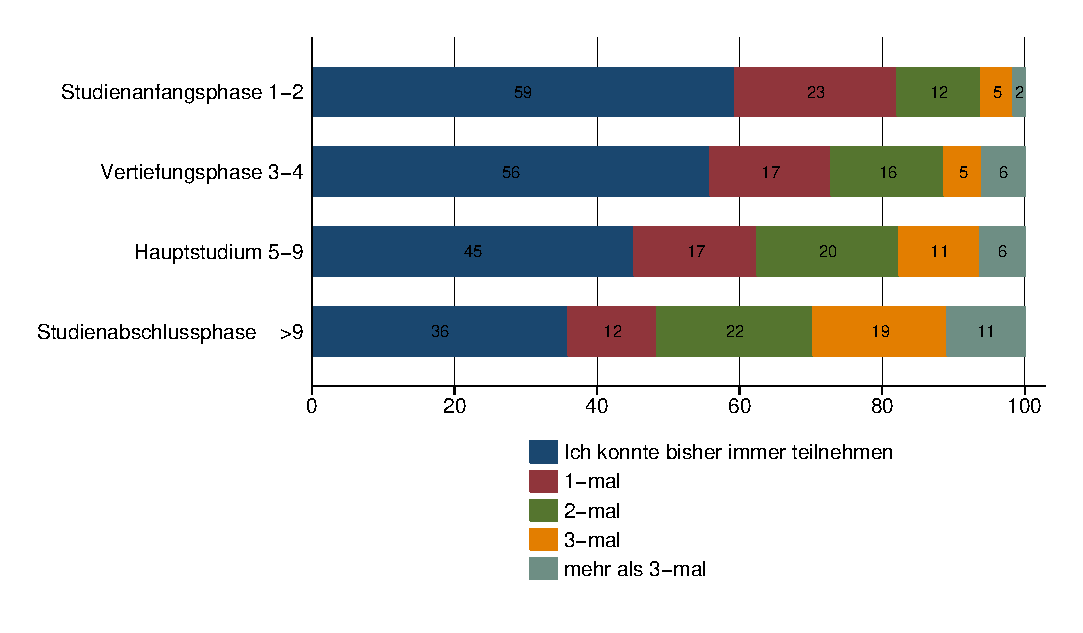
\includegraphics[
%  defaultresolution=72 !,
%  bmpsizefast=false
%]{image}
%\end{verbatim}
% \end{quote}
%
% \subsubsection{Hints}
%
% \begin{itemize}
% \item My version of \xfile{dvips.def} 1999/02/16 v3.0i defines
%       rules for the supported bitmap extensions, but does not
%       include them in the list of extensions that are tried
%       if the file name is not given with an extension.
%       In such a case, the list of extensions can be set
%       by \cs{DeclareGraphicsExtensions}, see \xpackage{grfguide}.
%       The following code just extends the list:
%       \begin{quote}
%\begin{verbatim}
%\makeatletter
%\g@addto@macro\Gin@extensions{,.bmp,.pcx,.msp}
%\makeatother
%\end{verbatim}
%       \end{quote}
% \item My version of \xfile{dvipdfm.def} 1998/11/24 vx.x misses
%       the graphics rule for PNG files. It can be added by:
%       \begin{quote}
%\begin{verbatim}
%\DeclareGraphicsRule{.png}{bmp}{.bb}{#1}
%\end{verbatim}
%       \end{quote}
%       See the previous issue to add the extension \xfile{.png} to the list
%       of extensions for package \xpackage{graphics}.
% \end{itemize}
%
% \subsubsection{Test program}
%
% There is a test program \xfile{bmpsize-test.tex}. Run it through
% \verb|latex|, \verb|pdflatex|, or \verb|pdftex|. Then given
% image files are inspected and the result is printed.
%
% \subsubsection{Interface for programmers}
%
% The macro names of the parsers are \verb|\bmpsize@read@|\meta{type}.
% Example: \cs{bmpsize@read@jpg} in case of JPEG.
%
% A parser sets the switch \cs{ifbmpsize@ok} to true, if it
% could successfully parse the image file.
% The width and height are returnd in \cs{bmpsize@width} and
% \cs{bmpsize@height}. If information about density is available,
% it is used to calculate width and height of the image, otherwise
% the values given by option \xoption{defaultresolution} is used.
% \xoption{resolution} overwrites the values in the image file.
%
% \subsection{Improved bitmap inclusion}
%
% Some drivers for package \xpackage{graphics} define the graphics
% type \xoption{bmp} for bitmap images. The code in the standard
% drivers for \xoption{dvips}, \xoption{dvipdfm}, and \xoption{dvipdfmx}
% is very basic and misses essential features of the
% package \xpackage{graphicx}. Therefore the code for bitmap
% inclusion is automatically rewritten by this package to add
% the following features:
% \begin{itemize}
% \item Support for \xoption{viewport} and \xoption{trim}.
% \item Support for \xoption{clip}.
% \item In case of \xoption{dvipdfm} and \xoption{dvipdfmx} the
%       bitmap images are reused and not included again if they
%       are used more than once.
% \end{itemize}
% However, there is a difference between \xoption{dvipdfm} and
% \xoption{dvipdfmx}, especially if images are reused. In the
% former case the reused box has width and height of 1bp, in the
% latter case its natural width. Thus the correct driver option must be given.
% \xoption{dvipdfm} and \xoption{dvipdfmx} are not equivalent.
%
% Older versions of \xoption{dvipdfmx} uses a size of 1in. However I do
% want to distinguish between versions of the same program. Therefore the
% support of these older versions has stopped with version 1.6 of this package.
% Use version dvipdfmx-20090708 or newer (some few versions before will
% probably also work, but I don't want to investigate this further).
%
% \StopEventually{
% }
%
% \section{Implementation}
%
% \subsection{Basic package \xpackage{bmpsize-base}}
%
%    Identification.
%    \begin{macrocode}
%<*base>
\ProvidesPackage{bmpsize-base}%
  [2009/09/04 v1.6 Basic part of bmpsize (HO)]%
%    \end{macrocode}
%    Modules of package \xpackage{fp} are used for calculations.
%    \begin{macrocode}
\RequirePackage{fp-basic}
\RequirePackage{fp-snap}
%    \end{macrocode}
%    Package \xpackage{fp} uses nested \cs{loop} structures.
%    That breaks with the plain-\TeX\ version of \cs{loop}.
%    Therefore we use the \LaTeX\ variant.
%    \begin{macro}{\@bmpsize@plain@loop}
%    \begin{macrocode}
\long\def\@bmpsize@plain@loop#1\repeat{%
  \def\iterate{%
    #1\relax
    \expandafter\iterate\fi
  }%
  \iterate
  \let\iterate\relax
}
%    \end{macrocode}
%    \end{macro}
%    \begin{macrocode}
\RequirePackage{pdftexcmds}[2007/11/11]
%    \end{macrocode}
%    \begin{macrocode}
\newif\ifbmpsize@ok
\let\@bmpsize@ok\bmpsize@oktrue

\newif\if@bmpsize@bigendian
\newif\if@bmpsize@absnum
\newif\if@bmpsize@user@resolution
\newif\if@bmpsize@fast
\@bmpsize@fasttrue

\def\@bmpsize@init{%
  \let\@bmpsize@org@plain@loop\loop
  \let\loop\@bmpsize@plain@loop
  \bmpsize@okfalse
  \@bmpsize@bigendiantrue
  \@bmpsize@absnumfalse
  \let\bmpsize@pixelwidth\relax
  \let\bmpsize@pixelheight\relax
  \let\bmpsize@pixelx\relax
  \let\bmpsize@pixely\relax
  \let\bmpsize@unit\relax
  \let\bmpsize@pixelxdenom\relax
  \let\bmpsize@pixelydenom\relax
  \let\bmpsize@orientation\relax
}

\def\@bmpsize@stop#1\@nil{}

\def\@bmpsize@loop#1{%
  #1%
  \@bmpsize@loop{#1}%
}
\def\@bmpsize@break#1\@bmpsize@loop#2{}

\def\@bmpsize@size#1#2#3{%
  \edef#3{\pdf@filesize{#1}}%
  \ifx#3\@empty
    \expandafter\@bmpsize@stop
  \fi
  \ifnum#3<#2\relax
    \expandafter\@bmpsize@stop
  \fi
}

\def\@bmpsize@read#1#2#3{%
  \edef\@bmpsize@buf{\pdf@filedump{#3}{#2}{#1}}%
  \edef\@bmpsize@temp{%
    \noexpand\@bmpsize@check@byte{#2}\@bmpsize@buf{}{}\noexpand\\%
  }%
  \@bmpsize@temp
}
\def\@bmpsize@fillbuf#1{%
  \ifx\@bmpsize@buf\@empty
    \expandafter\@firstofone
  \else
    \expandafter\@gobble
  \fi
  {%
    \edef\@bmpsize@buf{%
      \pdf@filedump{\bmpsize@offset}{\bmpsize@fillbuflength}{#1}%
    }%
    \ifx\@bmpsize@buf\@empty
      \expandafter\@bmpsize@stop
    \fi
    \edef\bmpsize@offset{\the\numexpr\bmpsize@offset+\bmpsize@fillbuflength}%
  }%
}
\def\bmpsize@fillbuflength{10}

\def\@bmpsize@append#1#2#3{%
  \edef#1{#2#3}%
}
\def\@bmpsize@pushback#1{%
  \edef\@bmpsize@buf{#1\@bmpsize@buf}%
}

\def\@bmpsize@iswhite#1{%
  \ifnum\pdf@strcmp{#1}{09}=\z@
  \else
    \ifnum\pdf@strcmp{#1}{0A}=\z@
    \else
      \ifnum\pdf@strcmp{#1}{0D}=\z@
      \else
        \ifnum\pdf@strcmp{#1}{20}=\z@
        \else
          1%
        \fi
      \fi
    \fi
  \fi
  \space
}
\def\@bmpsize@isdigit#1{%
  \ifnum\pdf@strcmp{#1}{30}<\z@
    1%
  \else
    \ifnum\pdf@strcmp{#1}{39}>\z@
      1%
    \fi
  \fi
  \space
}

\def\@bmpsize@check@byte#1#2#3{%
  \ifnum#1<\@ne
    \csname fi\endcsname
    \@bmpsize@cleanup@end
  \else
    \csname fi\endcsname
  \ifx!#2#3!%
    \csname fi\endcsname
    \@bmpsize@stop
  \else
    \csname fi\endcsname
    \expandafter\@bmpsize@check@byte\expandafter{\the\numexpr#1-1}%
}
\def\@bmpsize@cleanup@end#1\\{}

\def\@bmpsize@swap@maybe#1{%
  \if@bmpsize@bigendian
  \else
    \edef#1{\expandafter\@bmpsize@@swap#1\@empty\@empty\@empty\@empty}%
  \fi
}
\def\@bmpsize@@swap#1#2#3#4#5#6#7#8{%
  #7#8#5#6#3#4#1#2%
}

\def\@bmpsize@skip@one{%
  \edef\@bmpsize@buf{\expandafter\@gobbletwo\@bmpsize@buf}%
}
\def\@bmpsize@skip@two{%
  \edef\@bmpsize@buf{\expandafter\@gobblefour\@bmpsize@buf}%
}
\def\@bmpsize@skip@four{%
  \edef\@bmpsize@buf{%
    \expandafter\expandafter\expandafter\@gobblefour\expandafter
    \@gobblefour\@bmpsize@buf
  }%
}

\def\@bmpsize@grab#1#2{%
  \edef#1{\noexpand\@bmpsize@grab@byte#2=\@bmpsize@buf\noexpand\\}%
  \edef#1{#1}%
}
\def\@bmpsize@grab@byte#1=#2#3{%
  #2#3%
  \ifnum#1>\@ne
    \expandafter\@bmpsize@grab@byte\the\numexpr#1-1\expandafter=%
  \else
    \expandafter\@bmpsize@cleanup@end
  \fi
}

\def\@bmpsize@abs@maybe#1{%
  \let\@bmpsize@temp\relax
  \if@bmpsize@absnum
    \ifnum"\expandafter\@car#1\@nil>7 %
      \edef#1{\expandafter\@bmpsize@abs@byte#1\relax}%
      \ifnum\pdf@strcmp{#1}{7FFFFFFF}=\z@
        \let\@bmpsize@temp\@bmpsize@stop
      \else
        \def\@bmpsize@temp{\edef#1{\the\numexpr#1+1}}%
      \fi
    \fi
  \fi
}
\def\@bmpsize@abs@byte#1{%
  \ifx#1\relax
  \else
    \ifcase"0#1 %
      F\or E\or D\or C\or B\or A\or 9\or 8\or
      7\or 6\or 5\or 4\or 3\or 2\or 1\or 0%
    \fi
    \expandafter\@bmpsize@abs@byte
  \fi
}

\def\@bmpsize@num@one#1{%
  \@bmpsize@grab#11%
  \@bmpsize@abs@maybe#1%
  \edef#1{\number"#1}%
  \@bmpsize@temp
  \@bmpsize@skip@one
}
\def\@bmpsize@num@two#1{%
  \@bmpsize@grab#12%
  \@bmpsize@swap@maybe#1%
  \@bmpsize@abs@maybe#1%
  \edef#1{\number"#1}%
  \@bmpsize@temp
  \@bmpsize@skip@two
}
\def\@bmpsize@num@four#1{%
  \@bmpsize@grab#14%
  \@bmpsize@swap@maybe#1%
  \@bmpsize@abs@maybe#1%
  \ifnum\pdf@strcmp{#1}{7FFFFFFF}>\z@
    \expandafter\@bmpsize@stop
  \fi
  \edef#1{\number"#1}%
  \@bmpsize@temp
  \@bmpsize@skip@four
}

\def\@bmpsize@div#1#2#3{% #1 := #2/#3
  \FPdiv#1{#2}{#3}%
  \@bmpsize@beautify#1%
}
\def\@bmpsize@beautify#1{%
  \FPifint#1%
    \edef#1{\expandafter\@bmpsize@trunc#1.\@nil}%
  \else
    \edef#1{\expandafter\@bmpsize@cleanup@frac#1.\@nil}%
  \fi
}
\def\@bmpsize@trunc#1.#2\@nil{#1}
% #1 isn't an integer, thus we should have at least one
% necessary digit after the dot
\def\@bmpsize@cleanup@frac#1.#2#3.#4\@nil{%
  #1.#2%
  \ifx\\#3\\%
  \else
    \@bmpsize@cleanup@fracdigits#3000000000\@nil
  \fi
}
\def\@bmpsize@cleanup@fracdigits#1#2#3#4#5#6#7#8#9{%
  \ifcase#9 %
    \ifcase#8 %
      \ifcase#7 %
        \ifcase#6 %
          \ifcase#5 %
            \ifcase #4 %
              \ifcase #3 %
                \ifcase #2 %
                  \ifcase #1 %
                  \else
                    #1%
                  \fi
                \else
                  #1#2%
                \fi
              \else
                #1#2#3%
              \fi
            \else
              #1#2#3#4%
            \fi
          \else
            #1#2#3#4#5%
          \fi
        \else
          #1#2#3#4#5#6%
        \fi
      \else
        #1#2#3#4#5#6#7%
      \fi
    \else
      #1#2#3#4#5#6#7#8%
    \fi
  \else
    #1#2#3#4#5#6#7#8#9%
  \fi
  \@bmpsize@trunc.%
}

\def\@bmpsize@end{%
  \ifbmpsize@ok
    \ifx\bmpsize@pixelwidth\relax
      \bmpsize@okfalse
    \fi
    \ifx\bmpsize@pixelheight\relax
      \bmpsize@okfalse
    \fi
  \fi
  \ifbmpsize@ok
    \ifnum\bmpsize@pixelwidth>\z@
    \else
      \bmpsize@okfalse
    \fi
    \ifnum\bmpsize@pixelheight>\z@
    \else
      \bmpsize@okfalse
    \fi
  \fi
  \ifbmpsize@ok
    \ifcase 0%
      \ifx\bmpsize@pixelx\relax 1 \fi
      \ifx\bmpsize@pixely\relax 1 \fi
      \ifnum\bmpsize@pixelx>\z@\else 1 \fi
      \ifnum\bmpsize@pixely>\z@\else 1 \fi
      \ifx\bmpsize@pixelxdenom\relax
         \ifx\bmpsize@pixelydenom\relax\else 1 \fi
      \else
        \ifnum\bmpsize@pixelxdenom>\z@\else 1 \fi
      \fi
      \ifx\bmpsize@pixelydenom\relax
      \else
        \ifnum\bmpsize@pixelydenom>\z@\else 1 \fi
      \fi
    \else
      \let\bmpsize@pixelx\relax
      \let\bmpsize@pixely\relax
      \let\bmpsize@unit\relax
      \let\bmpsize@pixelxdenom\relax
      \let\bmpsize@pixelydenom\relax
    \fi
    \ifx\bmpsize@pixelxdenom\relax
    \else
      \@bmpsize@div\bmpsize@pixelx\bmpsize@pixelx\bmpsize@pixelxdenom
      \@bmpsize@div\bmpsize@pixely\bmpsize@pixely\bmpsize@pixelydenom
      \let\bmpsize@pixelxdenom\relax
      \let\bmpsize@pixelydenom\relax
    \fi
    \ifcase 0\ifx\bmpsize@unit\relax 1\fi
             \if@bmpsize@user@resolution 1\fi
             \relax
      \let\bmpsize@calc@unit\bmpsize@unit
      \let\bmpsize@calc@pixelx\bmpsize@pixelx
      \let\bmpsize@calc@pixely\bmpsize@pixely
    \else
      \let\bmpsize@calc@unit\bmpsize@unit@default
      \let\bmpsize@calc@pixelx\bmpsize@pixelx@default
      \let\bmpsize@calc@pixely\bmpsize@pixely@default
      \ifx\bmpsize@calc@pixely\Gin@exclamation
        \ifx\bmpsize@pixelx\relax
          \let\bmpsize@calc@pixely\bmpsize@calc@pixelx
        \else
          \FPdiv\bmpsize@calc@pixely\bmpsize@calc@pixelx\bmpsize@pixelx
          \FPmul\bmpsize@calc@pixely\bmpsize@calc@pixely\bmpsize@pixely
        \fi
      \else
        \ifx\bmpsize@calc@pixelx\Gin@exclamation
          \ifx\bmpsize@pixelx\relax
            \let\bmpsize@calc@pixelx\bmpsize@calc@pixely
          \else
            \FPdiv\bmpsize@calc@pixelx\bmpsize@calc@pixely\bmpsize@pixely
            \FPmul\bmpsize@calc@pixelx\bmpsize@calc@pixelx\bmpsize@pixelx
          \fi
        \fi
      \fi
    \fi
    \FPdiv\bmpsize@width\bmpsize@pixelwidth\bmpsize@calc@pixelx
    \FPdiv\bmpsize@height\bmpsize@pixelheight\bmpsize@calc@pixely
    % calculation of width and height in bp for package graphics
    % 1in = 72bp = 72.27pt, 72/72.27 = 8/8.03, 1pt = 65536sp
    \if@bmpsize@fast
      \edef\bmpsize@width{%
        \strip@pt\dimexpr.99626\dimexpr
        \bmpsize@width\dimexpr\bmpsize@calc@unit
      }%
      \edef\bmpsize@height{%
        \strip@pt\dimexpr.99626\dimexpr
        \bmpsize@height\dimexpr\bmpsize@calc@unit
      }%
    \else
      \edef\@bmpsize@temp{\number\dimexpr\bmpsize@calc@unit}%
      \ifnum\@bmpsize@temp>100000 %
        \FPmul\@bmpsize@temp\@bmpsize@temp{0.00001}%
        \def\@bmpsize@corr{100000}%
      \else
        \let\@bmpsize@corr\relax
      \fi
      \FPmul\bmpsize@width\bmpsize@width\@bmpsize@temp
      \FPmul\bmpsize@height\bmpsize@height\@bmpsize@temp
      \FPmul\bmpsize@width\bmpsize@width{8}%
      \FPmul\bmpsize@height\bmpsize@height{8}%
      \FPdiv\bmpsize@width\bmpsize@width{8.03}%
      \FPdiv\bmpsize@height\bmpsize@height{8.03}%
      \FPdiv\bmpsize@width\bmpsize@width{65536}%
      \FPdiv\bmpsize@height\bmpsize@height{65536}%
      \ifx\@bmpsize@corr\relax
      \else
        \FPmul\bmpsize@width\bmpsize@width\@bmpsize@corr
        \FPmul\bmpsize@height\bmpsize@height\@bmpsize@corr
      \fi
      \FPround\bmpsize@width\bmpsize@width{5}%
      \FPround\bmpsize@height\bmpsize@height{5}%
      \@bmpsize@beautify\bmpsize@width
      \@bmpsize@beautify\bmpsize@height
    \fi
  \fi
  \let\loop\@bmpsize@org@plain@loop
}
\def\bmpsize@unit@default{72.27pt}% more accurate than 1in
\def\bmpsize@pixelx@default{72}
\let\bmpsize@pixely@default\Gin@exclamation

\def\bmpsize@types{png,jpg,bmp,gif,tiff,pnm,pam,xpm,tga,pcx,msp,sgi}
%</base>
%    \end{macrocode}
%
% \subsection{Bitmap formats}
%
% \subsubsection{png}
%
%\iffalse
%<*ignore>
%\fi
%\begin{verbatim}
%begin png
%big-endian
%
%read 24 0
%grab 8        -> $temp
%check streq $temp [0x89 "PNG" 0x0D 0x0A 0x1A 0x0A]
%num 4         -> $length
%grab 4        -> $temp
%check streq $temp ["IHDR"]
%num 4         -> $pixelwidth
%num 4         -> $pixelheight
%ok
%assign numexpr(20 + $length) -> $offset
%loop
%  read 8 $offset
%  num 4       -> $length
%  grab 4      -> $temp
%  if streq $temp ["IDAT"]
%    stop
%  fi
%  if streq $temp ["pHYs"]
%    read 9 numexpr($offset + 8)
%    num 4     -> $pixelx
%    num 4     -> $pixely
%    grab 1     -> $temp
%    if numeq $temp 1
%      assign {100cm} -> $unit
%    fi
%    stop
%  fi
%  assign numexpr($offset + 12 + $length) -> $offset
%repeat
%end
%\end{verbatim}
%\iffalse
%</ignore>
%\fi
%    \begin{macro}{\bmpsize@read@png}
%    \begin{macrocode}
%<*base>
\def\bmpsize@read@png#1{%
  \@bmpsize@init
  \@bmpsize@bigendiantrue
  \@bmpsize@read{#1}{24}{0}%
  \@bmpsize@grab\bmpsize@temp{8}%
  \@bmpsize@skip@four
  \@bmpsize@skip@four
  \ifnum\pdf@strcmp{\bmpsize@temp}{89504E470D0A1A0A}=\z@
  \else
    \expandafter\@bmpsize@stop
  \fi
  \@bmpsize@num@four\bmpsize@length
  \@bmpsize@grab\bmpsize@temp{4}%
  \@bmpsize@skip@four
  \ifnum\pdf@strcmp{\bmpsize@temp}{49484452}=\z@
  \else
    \expandafter\@bmpsize@stop
  \fi
  \@bmpsize@num@four\bmpsize@pixelwidth
  \@bmpsize@num@four\bmpsize@pixelheight
  \@bmpsize@ok
  \edef\bmpsize@offset{\the\numexpr20+\bmpsize@length}%
  \@bmpsize@loop{%
    \@bmpsize@read{#1}{8}{\bmpsize@offset}%
    \@bmpsize@num@four\bmpsize@length
    \@bmpsize@grab\bmpsize@temp{4}%
    \@bmpsize@skip@four
    \ifnum\pdf@strcmp{\bmpsize@temp}{49444154}=\z@
      \expandafter\@firstofone
    \else
      \expandafter\@gobble
    \fi
    {%
      \@bmpsize@stop
    }%
    \ifnum\pdf@strcmp{\bmpsize@temp}{70485973}=\z@
      \expandafter\@firstofone
    \else
      \expandafter\@gobble
    \fi
    {%
      \@bmpsize@read{#1}{9}{\numexpr\bmpsize@offset+8\relax}%
      \@bmpsize@num@four\bmpsize@pixelx
      \@bmpsize@num@four\bmpsize@pixely
      \@bmpsize@grab\bmpsize@temp{1}%
      \@bmpsize@skip@one
      \ifnum\bmpsize@temp=1\relax
        \expandafter\@firstofone
      \else
        \expandafter\@gobble
      \fi
      {%
        \def\bmpsize@unit{100cm}%
      }%
      \@bmpsize@stop
    }%
    \edef\bmpsize@offset{\the\numexpr\bmpsize@offset+12+\bmpsize@length}%
  }%
  \@bmpsize@stop
  \@nil
  \@bmpsize@end
}%
%</base>
%    \end{macrocode}
%    \end{macro}
%
% \subsubsection{jpg}
%
%\iffalse
%<*ignore>
%\fi
%\begin{verbatim}
%begin jpg
%
%read 3 0
%grab 3      -> $temp % SOI and 0xFF
%check streq $temp [0xFF 0xD8 0xFF]
%assign {2} -> $offset
%assign {0} -> $exifdensity
%loop
%  read 4 $offset
%  grab 1    -> $temp
%  check streq $temp [0xFF]
%  num 1    -> $temp
%  if numeq $temp 0xDA % SOS
%    stop
%  fi
%  % look for JFIF APP0 segment
%  if numeq $temp 0xE0 % APP0
%    num 2       -> $length
%    if numeq $exifdensity 0
%      if numge $length 16 % a JFIF segment has 16 bytes at least
%        read 12 numexpr($offset + 4)
%        grab 5      -> $temp % identifier
%        if streq $temp ["JFIF" 0x0]
%          check numge $length 16
%          skip 2 % version
%          num 1       -> $temp % units
%          if numeq $temp 1
%            assign {72.27pt} -> $unit
%          else
%            if numeq $temp 2
%              assign {1cm} -> $unit
%            fi
%          fi
%          num 2    -> $pixelx
%          num 2    -> $pixely
%        fi
%      fi
%    fi
%  else
%    if numeq $temp 0xE1 % APP1
%      % look for Exif APP1 segment
%      num 2 -> $length
%      if numge $length 20 % identifier (6) + Tiff header (8) + first IFD (>=6)
%        read 20 numexpr($offset + 4)
%        grab 6 -> $temp
%        if streq $temp ["Exif" 0x0 0x0]
%          assign numexpr($offset + 10) -> $exifoffset
%          % read TIFF header
%          grab 2 -> $temp
%          if streq $temp ["II"]
%            little-endian
%          else
%            check streq $temp ["MM"]
%            % big-endian
%          fi
%          num 2 -> $temp
%          check numeq $temp 42
%          num 4 -> $temp % offset of first IFD
%          check numgt $temp 0
%          % read first IFD
%          assign numexpr($temp + $exifoffset) -> $off
%          read 2 $off
%          num 2 -> $entries
%          assign numexpr($off + 2) -> $off
%          loop
%            if numeq $entries 0
%              break
%            fi
%            assign numexpr($entries - 1) -> $entries
%            % entry format:
%            % 2 tag
%            % 2 field type
%            % 4 count
%            % 4 value/offset
%            read 12 $off
%            assign numexpr($off + 12) -> $off
%            num 2 -> $tag
%            if numeq $tag 296 % ResolutionUnit
%              skip 6 % type: 3 (short), count: 1
%              num 2 -> $temp
%              ifcase $temp
%              or % 1
%                clear $unit
%              or % 2
%                assign {72.27pt} -> $unit
%              or % 3
%                assign {1cm} -> $unit
%              else
%                clear $unit % unknown
%              fi
%              ifcase $temp
%              or % 1
%              or % 2
%                assign {1} -> $exifdensity
%              or % 3
%                assign {1} -> $exifdensity
%              else
%                assign $exifdensity -> $exifdensity
%              fi
%            fi
%            % 256 ImageWidth (use width of JPG part)
%            % 257 ImageHeight (use height of JPG part)
%            if numeq $tag 274 % Orientation
%              skip 6 % type: 3 (short), count: 1
%              num 2 -> $temp
%              if numge $temp 0 
%                if numle $temp 8
%                  assign $temp -> $orientation
%                fi
%              fi
%            fi
%            if numeq $tag 282 % XResolution
%              skip 6
%              num 4 -> $temp
%              read 8 numexpr($temp + $exifoffset)
%              num 4 -> $pixelx
%              num 4 -> $temp
%              if numeq $temp 1
%              else
%                assign numexpr($temp) -> $pixelxdenom
%                % div $pixelx $temp -> $pixelx
%              fi
%            fi
%            if numeq $tag 283 % YResolution
%              skip 6
%              num 4 -> $temp
%              read 8 numexpr($temp + $exifoffset)
%              num 4 -> $pixely
%              num 4 -> $temp
%              if numeq $temp 1
%              else
%                assign numexpr($temp) -> $pixelydenom
%                % div $pixely $temp -> $pixely
%              fi
%            fi
%          repeat
%          big-endian
%        fi
%      fi
%    else
%      assign numexpr($temp - 0xC0) -> $temp
%      ifcase $temp % SOF_0
%      or % SOF_1
%      or % SOF_2
%      or % SOF_3
%      or % DHT
%        assign {-1} -> $temp
%      or % SOF_5
%      or % SOF_6
%      or % SOF_7
%      or % JPG
%        assign {-1} -> $temp
%      or % SOF_9
%      or % SOF_10
%      or % SOF_11
%      or % DAC
%        assign {-1} -> $temp
%      or % SOF_13
%      or % SOF_14
%      or % SOF_15
%      else
%        assign {-1} -> $temp
%      fi
%      if numeq $temp -1
%      else
%        read 4 numexpr($offset + 5)
%        num 2  -> $pixelheight
%        num 2  -> $pixelwidth
%        if numeq $pixelheight 0
%          clear $pixelheight
%          stop
%        fi
%        ok
%        stop
%      fi
%      num 2 -> $length
%    fi
%  fi
%  assign numexpr($offset + $length + 2) -> $offset
%repeat
%end
%\end{verbatim}
%\iffalse
%</ignore>
%\fi
%    \begin{macro}{\bmpsize@read@jpg}
%    \begin{macrocode}
%<*base>
\def\bmpsize@read@jpg#1{%
  \@bmpsize@init
  \@bmpsize@read{#1}{3}{0}%
  \@bmpsize@grab\bmpsize@temp{3}%
  \@bmpsize@skip@two
  \@bmpsize@skip@one
  \ifnum\pdf@strcmp{\bmpsize@temp}{FFD8FF}=\z@
  \else
    \expandafter\@bmpsize@stop
  \fi
  \def\bmpsize@offset{2}%
  \def\bmpsize@exifdensity{0}%
  \@bmpsize@loop{%
    \@bmpsize@read{#1}{4}{\bmpsize@offset}%
    \@bmpsize@grab\bmpsize@temp{1}%
    \@bmpsize@skip@one
    \ifnum\pdf@strcmp{\bmpsize@temp}{FF}=\z@
    \else
      \expandafter\@bmpsize@stop
    \fi
    \@bmpsize@num@one\bmpsize@temp
    \ifnum\bmpsize@temp=218\relax
      \expandafter\@firstofone
    \else
      \expandafter\@gobble
    \fi
    {%
      \@bmpsize@stop
    }%
    \ifnum\bmpsize@temp=224\relax
      \expandafter\@firstoftwo
    \else
      \expandafter\@secondoftwo
    \fi
    {%
      \@bmpsize@num@two\bmpsize@length
      \ifnum\bmpsize@exifdensity=0\relax
        \expandafter\@firstofone
      \else
        \expandafter\@gobble
      \fi
      {%
        \unless\ifnum\bmpsize@length<16\relax
          \expandafter\@firstofone
        \else
          \expandafter\@gobble
        \fi
        {%
          \@bmpsize@read{#1}{12}{\numexpr\bmpsize@offset+4\relax}%
          \@bmpsize@grab\bmpsize@temp{5}%
          \@bmpsize@skip@four
          \@bmpsize@skip@one
          \ifnum\pdf@strcmp{\bmpsize@temp}{4A46494600}=\z@
            \expandafter\@firstofone
          \else
            \expandafter\@gobble
          \fi
          {%
            \ifnum\bmpsize@length<16\relax
              \expandafter\@bmpsize@stop
            \fi
            \@bmpsize@skip@two
            \@bmpsize@num@one\bmpsize@temp
            \ifnum\bmpsize@temp=1\relax
              \expandafter\@firstoftwo
            \else
              \expandafter\@secondoftwo
            \fi
            {%
              \def\bmpsize@unit{72.27pt}%
            }{%
              \ifnum\bmpsize@temp=2\relax
                \expandafter\@firstofone
              \else
                \expandafter\@gobble
              \fi
              {%
                \def\bmpsize@unit{1cm}%
              }%
            }%
            \@bmpsize@num@two\bmpsize@pixelx
            \@bmpsize@num@two\bmpsize@pixely
          }%
        }%
      }%
    }{%
      \ifnum\bmpsize@temp=225\relax
        \expandafter\@firstoftwo
      \else
        \expandafter\@secondoftwo
      \fi
      {%
        \@bmpsize@num@two\bmpsize@length
        \unless\ifnum\bmpsize@length<20\relax
          \expandafter\@firstofone
        \else
          \expandafter\@gobble
        \fi
        {%
          \@bmpsize@read{#1}{20}{\numexpr\bmpsize@offset+4\relax}%
          \@bmpsize@grab\bmpsize@temp{6}%
          \@bmpsize@skip@four
          \@bmpsize@skip@two
          \ifnum\pdf@strcmp{\bmpsize@temp}{457869660000}=\z@
            \expandafter\@firstofone
          \else
            \expandafter\@gobble
          \fi
          {%
            \edef\bmpsize@exifoffset{\the\numexpr\bmpsize@offset+10}%
            \@bmpsize@grab\bmpsize@temp{2}%
            \@bmpsize@skip@two
            \ifnum\pdf@strcmp{\bmpsize@temp}{4949}=\z@
              \expandafter\@firstoftwo
            \else
              \expandafter\@secondoftwo
            \fi
            {%
              \@bmpsize@bigendianfalse
            }{%
              \ifnum\pdf@strcmp{\bmpsize@temp}{4D4D}=\z@
              \else
                \expandafter\@bmpsize@stop
              \fi
            }%
            \@bmpsize@num@two\bmpsize@temp
            \ifnum\bmpsize@temp=42\relax
            \else
              \expandafter\@bmpsize@stop
            \fi
            \@bmpsize@num@four\bmpsize@temp
            \ifnum\bmpsize@temp>0\relax
            \else
              \expandafter\@bmpsize@stop
            \fi
            \edef\bmpsize@off{\the\numexpr\bmpsize@temp+\bmpsize@exifoffset}%
            \@bmpsize@read{#1}{2}{\bmpsize@off}%
            \@bmpsize@num@two\bmpsize@entries
            \edef\bmpsize@off{\the\numexpr\bmpsize@off+2}%
            \@bmpsize@loop{%
              \ifnum\bmpsize@entries=0\relax
                \expandafter\@firstofone
              \else
                \expandafter\@gobble
              \fi
              {%
                \@bmpsize@break
              }%
              \edef\bmpsize@entries{\the\numexpr\bmpsize@entries-1}%
              \@bmpsize@read{#1}{12}{\bmpsize@off}%
              \edef\bmpsize@off{\the\numexpr\bmpsize@off+12}%
              \@bmpsize@num@two\bmpsize@tag
              \ifnum\bmpsize@tag=296\relax
                \expandafter\@firstofone
              \else
                \expandafter\@gobble
              \fi
              {%
                \@bmpsize@skip@four
                \@bmpsize@skip@two
                \@bmpsize@num@two\bmpsize@temp
                \ifcase\bmpsize@temp\relax
                \or
                  \let\bmpsize@unit\relax
                \or
                  \def\bmpsize@unit{72.27pt}%
                \or
                  \def\bmpsize@unit{1cm}%
                \else
                  \let\bmpsize@unit\relax
                \fi
                \ifcase\bmpsize@temp\relax
                \or
                \or
                  \def\bmpsize@exifdensity{1}%
                \or
                  \def\bmpsize@exifdensity{1}%
                \else
                  \let\bmpsize@exifdensity\bmpsize@exifdensity
                \fi
              }%
              \ifnum\bmpsize@tag=274\relax
                \expandafter\@firstofone
              \else
                \expandafter\@gobble
              \fi
              {%
                \@bmpsize@skip@four
                \@bmpsize@skip@two
                \@bmpsize@num@two\bmpsize@temp
                \unless\ifnum\bmpsize@temp<0\relax
                  \expandafter\@firstofone
                \else
                  \expandafter\@gobble
                \fi
                {%
                  \unless\ifnum\bmpsize@temp>8\relax
                    \expandafter\@firstofone
                  \else
                    \expandafter\@gobble
                  \fi
                  {%
                    \let\bmpsize@orientation\bmpsize@temp
                  }%
                }%
              }%
              \ifnum\bmpsize@tag=282\relax
                \expandafter\@firstofone
              \else
                \expandafter\@gobble
              \fi
              {%
                \@bmpsize@skip@four
                \@bmpsize@skip@two
                \@bmpsize@num@four\bmpsize@temp
                \@bmpsize@read{#1}{8}{\numexpr\bmpsize@temp+\bmpsize@exifoffset\relax}%
                \@bmpsize@num@four\bmpsize@pixelx
                \@bmpsize@num@four\bmpsize@temp
                \ifnum\bmpsize@temp=1\relax
                  \expandafter\@gobble
                \else
                  \expandafter\@firstofone
                \fi
                {%
                  \edef\bmpsize@pixelxdenom{\the\numexpr\bmpsize@temp}%
                }%
              }%
              \ifnum\bmpsize@tag=283\relax
                \expandafter\@firstofone
              \else
                \expandafter\@gobble
              \fi
              {%
                \@bmpsize@skip@four
                \@bmpsize@skip@two
                \@bmpsize@num@four\bmpsize@temp
                \@bmpsize@read{#1}{8}{\numexpr\bmpsize@temp+\bmpsize@exifoffset\relax}%
                \@bmpsize@num@four\bmpsize@pixely
                \@bmpsize@num@four\bmpsize@temp
                \ifnum\bmpsize@temp=1\relax
                  \expandafter\@gobble
                \else
                  \expandafter\@firstofone
                \fi
                {%
                  \edef\bmpsize@pixelydenom{\the\numexpr\bmpsize@temp}%
                }%
              }%
            }%
            \@bmpsize@bigendiantrue
          }%
        }%
      }{%
        \edef\bmpsize@temp{\the\numexpr\bmpsize@temp-192}%
        \ifcase\bmpsize@temp\relax
        \or
        \or
        \or
        \or
          \def\bmpsize@temp{-1}%
        \or
        \or
        \or
        \or
          \def\bmpsize@temp{-1}%
        \or
        \or
        \or
        \or
          \def\bmpsize@temp{-1}%
        \or
        \or
        \or
        \else
          \def\bmpsize@temp{-1}%
        \fi
        \ifnum\bmpsize@temp=-1\relax
          \expandafter\@gobble
        \else
          \expandafter\@firstofone
        \fi
        {%
          \@bmpsize@read{#1}{4}{\numexpr\bmpsize@offset+5\relax}%
          \@bmpsize@num@two\bmpsize@pixelheight
          \@bmpsize@num@two\bmpsize@pixelwidth
          \ifnum\bmpsize@pixelheight=0\relax
            \expandafter\@firstofone
          \else
            \expandafter\@gobble
          \fi
          {%
            \let\bmpsize@pixelheight\relax
            \@bmpsize@stop
          }%
          \@bmpsize@ok
          \@bmpsize@stop
        }%
        \@bmpsize@num@two\bmpsize@length
      }%
    }%
    \edef\bmpsize@offset{\the\numexpr\bmpsize@offset+\bmpsize@length+2}%
  }%
  \@bmpsize@stop
  \@nil
  \@bmpsize@end
}%
%</base>
%    \end{macrocode}
%    \end{macro}
%
% \subsubsection{bmp}
%
%\iffalse
%<*ignore>
%\fi
%\begin{verbatim}
%begin bmp
%little-endian
%
%read 26 0
%grab 2 -> $temp
%check streq $temp ["BM"]
%skip 12
%% header size is 4 bytes in V3+, unknown for V1, V2,
%% known header sizes fit in 2 bytes
%num 2   -> $temp
%if numeq $temp 12 % V1
%  skip 2
%  num 2 -> $pixelwidth
%  num 2 -> $pixelheight
%  % no resolution entries
%  ok
%  stop
%fi
%if numeq $temp 64 % V2
%  skip 2
%  num 2 -> $pixelwidth
%  num 2 -> $pixelheight
%  % missing specification for resolution
%  ok
%  stop
%fi
%% V3, V4, V5
%skip 2
%num 4 -> $pixelwidth
%absnum 4 -> $pixelheight
%ok
%read 8 38
%num 4 -> $pixelx
%num 4 -> $pixely
%assign {100cm} -> $unit
%end
%\end{verbatim}
%\iffalse
%</ignore>
%\fi
%    \begin{macro}{\bmpsize@read@bmp}
%    \begin{macrocode}
%<*base>
\def\bmpsize@read@bmp#1{%
  \@bmpsize@init
  \@bmpsize@bigendianfalse
  \@bmpsize@read{#1}{26}{0}%
  \@bmpsize@grab\bmpsize@temp{2}%
  \@bmpsize@skip@two
  \ifnum\pdf@strcmp{\bmpsize@temp}{424D}=\z@
  \else
    \expandafter\@bmpsize@stop
  \fi
  \@bmpsize@skip@four
  \@bmpsize@skip@four
  \@bmpsize@skip@four
  \@bmpsize@num@two\bmpsize@temp
  \ifnum\bmpsize@temp=12\relax
    \expandafter\@firstofone
  \else
    \expandafter\@gobble
  \fi
  {%
    \@bmpsize@skip@two
    \@bmpsize@num@two\bmpsize@pixelwidth
    \@bmpsize@num@two\bmpsize@pixelheight
    \@bmpsize@ok
    \@bmpsize@stop
  }%
  \ifnum\bmpsize@temp=64\relax
    \expandafter\@firstofone
  \else
    \expandafter\@gobble
  \fi
  {%
    \@bmpsize@skip@two
    \@bmpsize@num@two\bmpsize@pixelwidth
    \@bmpsize@num@two\bmpsize@pixelheight
    \@bmpsize@ok
    \@bmpsize@stop
  }%
  \@bmpsize@skip@two
  \@bmpsize@num@four\bmpsize@pixelwidth
  \@bmpsize@absnumtrue
  \@bmpsize@num@four\bmpsize@pixelheight
  \@bmpsize@absnumfalse
  \@bmpsize@ok
  \@bmpsize@read{#1}{8}{38}%
  \@bmpsize@num@four\bmpsize@pixelx
  \@bmpsize@num@four\bmpsize@pixely
  \def\bmpsize@unit{100cm}%
  \@bmpsize@stop
  \@nil
  \@bmpsize@end
}%
%</base>
%    \end{macrocode}
%    \end{macro}
%
% \subsubsection{gif}
%
%\iffalse
%<*ignore>
%\fi
%\begin{verbatim}
%begin gif
%little-endian
%
%% Header
%read 13 0
%grab 3      -> $temp
%check streq $temp ["GIF"]
%skip 3      % version
%
%% Logical Screen Descriptor
%num 2       -> $pixelwidth
%num 2       -> $pixelheight
%skip 2
%num 1       -> $temp % Pixel Aspect Ratio
%if numeq $temp 0
%else
%  assign numexpr($temp + 15) -> $pixelx
%  assign {64}     -> $pixely
%fi
%ok
%end
%\end{verbatim}
%\iffalse
%</ignore>
%\fi
%    \begin{macro}{\bmpsize@read@gif}
%    \begin{macrocode}
%<*base>
\def\bmpsize@read@gif#1{%
  \@bmpsize@init
  \@bmpsize@bigendianfalse
  \@bmpsize@read{#1}{13}{0}%
  \@bmpsize@grab\bmpsize@temp{3}%
  \@bmpsize@skip@two
  \@bmpsize@skip@one
  \ifnum\pdf@strcmp{\bmpsize@temp}{474946}=\z@
  \else
    \expandafter\@bmpsize@stop
  \fi
  \@bmpsize@skip@two
  \@bmpsize@skip@one
  \@bmpsize@num@two\bmpsize@pixelwidth
  \@bmpsize@num@two\bmpsize@pixelheight
  \@bmpsize@skip@two
  \@bmpsize@num@one\bmpsize@temp
  \ifnum\bmpsize@temp=0\relax
    \expandafter\@gobble
  \else
    \expandafter\@firstofone
  \fi
  {%
    \edef\bmpsize@pixelx{\the\numexpr\bmpsize@temp+15}%
    \def\bmpsize@pixely{64}%
  }%
  \@bmpsize@ok
  \@bmpsize@stop
  \@nil
  \@bmpsize@end
}%
%</base>
%    \end{macrocode}
%    \end{macro}
%
% \subsubsection{tiff}
%
%\iffalse
%<*ignore>
%\fi
%\begin{verbatim}
%begin tiff
%% defaults
%assign {72.27pt} -> $unit
%
%% Image File Header
%read 8 0
%grab 2 -> $temp
%if streq $temp ["II"]
%  little-endian
%else
%  check streq $temp ["MM"]
%  big-endian
%fi
%num 2 -> $temp
%check numeq $temp 42
%num 4 -> $offset % first IFD (Image File Directory)
%
%% First IFD
%read 2 $offset
%assign numexpr($offset + 2) -> $offset
%num 2 -> $entries
%ok % must rely on checks at the end
%loop
%  if numeq $entries 0
%    stop
%  fi
%  assign numexpr($entries - 1) -> $entries
%  % entry format:
%  % 2 tag
%  % 2 field type
%  % 4 count
%  % 4 value/offset
%  read 12 $offset
%  assign numexpr($offset + 12) -> $offset
%  num 2 -> $tag % tag
%  if numeq $temp 296 % ResolutionUnit
%    skip 6 % type: 3 (short), count: 1
%    num 2 -> $temp
%    ifcase $temp
%    or % 1
%      clear $unit
%    or % 2
%      assign {72.27pt} -> $unit
%    or % 3
%      assign {1cm} -> $unit
%    else
%      clear $unit
%    fi
%  fi
%  if numeq $tag 256 % ImageWidth
%    skip 6
%    num 4 -> $pixelwidth
%  fi
%  if numeq $tag 257 % ImageLength
%    skip 6
%    num 4 -> $pixelheight
%  fi
%  if numeq $tag 282 % XResolution
%    skip 6
%    num 4 -> $temp
%    read 8 $temp
%    num 4 -> $pixelx
%    num 4 -> $temp
%    if numeq $temp 1
%    else
%      assign numexpr($temp) -> $pixelxdenom
%      % div $pixelx $temp -> $pixelx
%    fi
%  fi
%  if numeq $tag 283 % YResolution
%    skip 6
%    num 4 -> $temp
%    read 8 $temp
%    num 4 -> $pixely
%    num 4 -> $temp
%    if numeq $temp 1
%    else
%      assign numexpr($temp) -> $pixelydenom
%      % div $pixely $temp -> $pixely
%    fi
%  fi
%repeat
%end
%\end{verbatim}
%\iffalse
%</ignore>
%\fi
%    \begin{macro}{\bmpsize@read@tiff}
%    \begin{macrocode}
%<*base>
\def\bmpsize@read@tiff#1{%
  \@bmpsize@init
  \def\bmpsize@unit{72.27pt}%
  \@bmpsize@read{#1}{8}{0}%
  \@bmpsize@grab\bmpsize@temp{2}%
  \@bmpsize@skip@two
  \ifnum\pdf@strcmp{\bmpsize@temp}{4949}=\z@
    \expandafter\@firstoftwo
  \else
    \expandafter\@secondoftwo
  \fi
  {%
    \@bmpsize@bigendianfalse
  }{%
    \ifnum\pdf@strcmp{\bmpsize@temp}{4D4D}=\z@
    \else
      \expandafter\@bmpsize@stop
    \fi
    \@bmpsize@bigendiantrue
  }%
  \@bmpsize@num@two\bmpsize@temp
  \ifnum\bmpsize@temp=42\relax
  \else
    \expandafter\@bmpsize@stop
  \fi
  \@bmpsize@num@four\bmpsize@offset
  \@bmpsize@read{#1}{2}{\bmpsize@offset}%
  \edef\bmpsize@offset{\the\numexpr\bmpsize@offset+2}%
  \@bmpsize@num@two\bmpsize@entries
  \@bmpsize@ok
  \@bmpsize@loop{%
    \ifnum\bmpsize@entries=0\relax
      \expandafter\@firstofone
    \else
      \expandafter\@gobble
    \fi
    {%
      \@bmpsize@stop
    }%
    \edef\bmpsize@entries{\the\numexpr\bmpsize@entries-1}%
    \@bmpsize@read{#1}{12}{\bmpsize@offset}%
    \edef\bmpsize@offset{\the\numexpr\bmpsize@offset+12}%
    \@bmpsize@num@two\bmpsize@tag
    \ifnum\bmpsize@temp=296\relax
      \expandafter\@firstofone
    \else
      \expandafter\@gobble
    \fi
    {%
      \@bmpsize@skip@four
      \@bmpsize@skip@two
      \@bmpsize@num@two\bmpsize@temp
      \ifcase\bmpsize@temp\relax
      \or
        \let\bmpsize@unit\relax
      \or
        \def\bmpsize@unit{72.27pt}%
      \or
        \def\bmpsize@unit{1cm}%
      \else
        \let\bmpsize@unit\relax
      \fi
    }%
    \ifnum\bmpsize@tag=256\relax
      \expandafter\@firstofone
    \else
      \expandafter\@gobble
    \fi
    {%
      \@bmpsize@skip@four
      \@bmpsize@skip@two
      \@bmpsize@num@four\bmpsize@pixelwidth
    }%
    \ifnum\bmpsize@tag=257\relax
      \expandafter\@firstofone
    \else
      \expandafter\@gobble
    \fi
    {%
      \@bmpsize@skip@four
      \@bmpsize@skip@two
      \@bmpsize@num@four\bmpsize@pixelheight
    }%
    \ifnum\bmpsize@tag=282\relax
      \expandafter\@firstofone
    \else
      \expandafter\@gobble
    \fi
    {%
      \@bmpsize@skip@four
      \@bmpsize@skip@two
      \@bmpsize@num@four\bmpsize@temp
      \@bmpsize@read{#1}{8}{\bmpsize@temp}%
      \@bmpsize@num@four\bmpsize@pixelx
      \@bmpsize@num@four\bmpsize@temp
      \ifnum\bmpsize@temp=1\relax
        \expandafter\@gobble
      \else
        \expandafter\@firstofone
      \fi
      {%
        \edef\bmpsize@pixelxdenom{\the\numexpr\bmpsize@temp}%
      }%
    }%
    \ifnum\bmpsize@tag=283\relax
      \expandafter\@firstofone
    \else
      \expandafter\@gobble
    \fi
    {%
      \@bmpsize@skip@four
      \@bmpsize@skip@two
      \@bmpsize@num@four\bmpsize@temp
      \@bmpsize@read{#1}{8}{\bmpsize@temp}%
      \@bmpsize@num@four\bmpsize@pixely
      \@bmpsize@num@four\bmpsize@temp
      \ifnum\bmpsize@temp=1\relax
        \expandafter\@gobble
      \else
        \expandafter\@firstofone
      \fi
      {%
        \edef\bmpsize@pixelydenom{\the\numexpr\bmpsize@temp}%
      }%
    }%
  }%
  \@bmpsize@stop
  \@nil
  \@bmpsize@end
}%
%</base>
%    \end{macrocode}
%    \end{macro}
%
% \subsubsection{pnm}
%
%\iffalse
%<*ignore>
%\fi
%\begin{verbatim}
%begin pnm
%assign {0} -> $offset
%read 3 $offset
%assign {3} -> $offset
%grab 1 -> $temp
%check streq $temp ["P"]
%grab 1 -> $temp
%check strge $temp ["1"]
%check strle $temp ["6"]
%% ensure one white space
%grab 1 -> $temp
%if iswhite $temp
%else
%  stop
%fi
%loop
%  % skip white space
%  fillbuf
%  grab 1 -> $temp
%  if iswhite $temp
%  else
%    if streq $temp ["#"]
%      % ignore comments
%      loop
%        fillbuf
%        grab 1 -> $temp
%        if streq $temp [0x0A]
%          break
%        else
%          if streq $temp [0x0D]
%            break
%          fi
%        fi
%      repeat
%    else
%      pushback $temp
%      break
%    fi
%  fi
%repeat
%assign {} -> $tempnum
%loop
%  fillbuf
%  grab 1 -> $temp
%  if isdigit $temp
%    append $tempnum $temp -> $tempnum
%  else
%    if iswhite $temp
%      break
%    else
%      stop
%    fi
%  fi
%repeat
%assign unescapehex($tempnum) -> $pixelwidth
%loop
%  fillbuf
%  grab 1 -> $temp
%  if iswhite $temp
%  else
%    pushback $temp
%    break
%  fi
%repeat
%assign {} -> $tempnum
%loop
%  fillbuf
%  grab 1 -> $temp
%  if isdigit $temp
%    append $tempnum $temp -> $tempnum
%  else
%    if iswhite $temp
%      break
%    else
%      stop
%    fi
%  fi
%repeat
%assign unescapehex($tempnum) -> $pixelheight
%ok
%end
%\end{verbatim}
%\iffalse
%</ignore>
%\fi
%    \begin{macro}{\bmpsize@read@pnm}
%    \begin{macrocode}
%<*base>
\def\bmpsize@read@pnm#1{%
  \@bmpsize@init
  \def\bmpsize@offset{0}%
  \@bmpsize@read{#1}{3}{\bmpsize@offset}%
  \def\bmpsize@offset{3}%
  \@bmpsize@grab\bmpsize@temp{1}%
  \@bmpsize@skip@one
  \ifnum\pdf@strcmp{\bmpsize@temp}{50}=\z@
  \else
    \expandafter\@bmpsize@stop
  \fi
  \@bmpsize@grab\bmpsize@temp{1}%
  \@bmpsize@skip@one
  \ifnum\pdf@strcmp{\bmpsize@temp}{31}<\z@
    \expandafter\@bmpsize@stop
  \fi
  \ifnum\pdf@strcmp{\bmpsize@temp}{36}>\z@
    \expandafter\@bmpsize@stop
  \fi
  \@bmpsize@grab\bmpsize@temp{1}%
  \@bmpsize@skip@one
  \ifcase 0\@bmpsize@iswhite\bmpsize@temp
    \expandafter\@gobble
  \else
    \expandafter\@firstofone
  \fi
  {%
    \@bmpsize@stop
  }%
  \@bmpsize@loop{%
    \@bmpsize@fillbuf{#1}%
    \@bmpsize@grab\bmpsize@temp{1}%
    \@bmpsize@skip@one
    \ifcase 0\@bmpsize@iswhite\bmpsize@temp
      \expandafter\@gobble
    \else
      \expandafter\@firstofone
    \fi
    {%
      \ifnum\pdf@strcmp{\bmpsize@temp}{23}=\z@
        \expandafter\@firstoftwo
      \else
        \expandafter\@secondoftwo
      \fi
      {%
        \@bmpsize@loop{%
          \@bmpsize@fillbuf{#1}%
          \@bmpsize@grab\bmpsize@temp{1}%
          \@bmpsize@skip@one
          \ifnum\pdf@strcmp{\bmpsize@temp}{0A}=\z@
            \expandafter\@firstoftwo
          \else
            \expandafter\@secondoftwo
          \fi
          {%
            \@bmpsize@break
          }{%
            \ifnum\pdf@strcmp{\bmpsize@temp}{0D}=\z@
              \expandafter\@firstofone
            \else
              \expandafter\@gobble
            \fi
            {%
              \@bmpsize@break
            }%
          }%
        }%
      }{%
        \@bmpsize@pushback\bmpsize@temp
        \@bmpsize@break
      }%
    }%
  }%
  \def\bmpsize@tempnum{}%
  \@bmpsize@loop{%
    \@bmpsize@fillbuf{#1}%
    \@bmpsize@grab\bmpsize@temp{1}%
    \@bmpsize@skip@one
    \ifcase 0\@bmpsize@isdigit\bmpsize@temp
      \expandafter\@firstoftwo
    \else
      \expandafter\@secondoftwo
    \fi
    {%
      \@bmpsize@append\bmpsize@tempnum\bmpsize@tempnum\bmpsize@temp
    }{%
      \ifcase 0\@bmpsize@iswhite\bmpsize@temp
        \expandafter\@firstoftwo
      \else
        \expandafter\@secondoftwo
      \fi
      {%
        \@bmpsize@break
      }{%
        \@bmpsize@stop
      }%
    }%
  }%
  \edef\bmpsize@pixelwidth{\pdf@unescapehex{\bmpsize@tempnum}}%
  \@bmpsize@loop{%
    \@bmpsize@fillbuf{#1}%
    \@bmpsize@grab\bmpsize@temp{1}%
    \@bmpsize@skip@one
    \ifcase 0\@bmpsize@iswhite\bmpsize@temp
      \expandafter\@gobble
    \else
      \expandafter\@firstofone
    \fi
    {%
      \@bmpsize@pushback\bmpsize@temp
      \@bmpsize@break
    }%
  }%
  \def\bmpsize@tempnum{}%
  \@bmpsize@loop{%
    \@bmpsize@fillbuf{#1}%
    \@bmpsize@grab\bmpsize@temp{1}%
    \@bmpsize@skip@one
    \ifcase 0\@bmpsize@isdigit\bmpsize@temp
      \expandafter\@firstoftwo
    \else
      \expandafter\@secondoftwo
    \fi
    {%
      \@bmpsize@append\bmpsize@tempnum\bmpsize@tempnum\bmpsize@temp
    }{%
      \ifcase 0\@bmpsize@iswhite\bmpsize@temp
        \expandafter\@firstoftwo
      \else
        \expandafter\@secondoftwo
      \fi
      {%
        \@bmpsize@break
      }{%
        \@bmpsize@stop
      }%
    }%
  }%
  \edef\bmpsize@pixelheight{\pdf@unescapehex{\bmpsize@tempnum}}%
  \@bmpsize@ok
  \@bmpsize@stop
  \@nil
  \@bmpsize@end
}%
%</base>
%    \end{macrocode}
%    \end{macro}
%
% \subsubsection{pam}
%
%\iffalse
%<*ignore>
%\fi
%\begin{verbatim}
%begin pam
%read 3 0
%assign {3} -> $offset
%assign $offset -> $off
%grab 3 -> $temp
%check streq $temp ["P7" 0x0A]
%loop
%  fillbuf
%  grab 1 -> $temp
%  if iswhite $temp
%    % ignore white space
%    assign numexpr($off + 1) -> $off
%  else
%    if streq $temp ["#"]
%      % ignore comment line
%      assign numexpr($off + 1) -> $off
%      loop
%        fillbuf
%        grab 1 -> $temp
%        assign numexpr($off + 1) -> $off
%        if streq $temp [0x0A]
%          break
%        fi
%      repeat
%    else
%      read 6 $off
%      assign numexpr($off + 6) -> $offset
%      grab 5 -> $head
%      if streq $head ["WIDTH"]
%        assign numexpr($off + 5) -> $off
%        % skip white space
%        loop
%          fillbuf
%          grab 1 -> $temp
%          if iswhite $temp
%            assign numexpr($off + 1) -> $off
%          else
%            if isdigit $temp
%              assign numexpr($off + 1) -> $off
%              break
%            else
%              % error
%              stop
%            fi
%          fi
%        repeat
%        % read number
%        assign $temp -> $tempnum
%        loop
%          fillbuf
%          grab 1 -> $temp
%          if isdigit $temp
%            assign numexpr($off + 1) -> $off
%            append $tempnum $temp -> $tempnum
%          else
%            pushback $temp
%            break
%          fi
%        repeat
%        % skip to end of line
%        loop
%          fillbuf
%          grab 1 -> $temp
%          assign numexpr($off + 1) -> $off
%          if streq $temp [0x0A]
%            break
%          fi
%        repeat
%        assign unescapehex($tempnum) -> $pixelwidth
%      else
%        grab 1 -> $temp
%        append $head $temp -> $head
%        if streq $head ["ENDHDR"]
%          % last header line
%          ok
%          stop
%        else
%          if streq $head ["HEIGHT"]
%            assign numexpr($off + 6) -> $off
%            % skip white space
%            loop
%              fillbuf
%              grab 1 -> $temp
%              if iswhite $temp
%                assign numexpr($off + 1) -> $off
%              else
%                if isdigit $temp
%                  assign numexpr($off + 1) -> $off
%                  break
%                else
%                  % error
%                  stop
%                fi
%              fi
%            repeat
%            % read number
%            assign $temp -> $tempnum
%            loop
%              fillbuf
%              grab 1 -> $temp
%              if isdigit $temp
%                assign numexpr($off + 1) -> $off
%                append $tempnum $temp -> $tempnum
%              else
%                pushback $temp
%                break
%              fi
%            repeat
%            % skip to end of line
%            loop
%              fillbuf
%              grab 1 -> $temp
%              assign numexpr($off + 1) -> $off
%              if streq $temp [0x0A]
%                break
%              fi
%            repeat
%            assign unescapehex($tempnum) -> $pixelheight
%          else
%            % ignore unknown header line
%            pushback $head
%            loop
%              fillbuf
%              grab 1 -> $temp
%              assign numexpr($off + 1) -> $off
%              if streq $temp [0x0A]
%                break
%              fi
%            repeat
%          fi
%        fi
%      fi
%    fi
%  fi
%repeat
%end
%\end{verbatim}
%\iffalse
%</ignore>
%\fi
%    \begin{macro}{\bmpsize@read@pam}
%    \begin{macrocode}
%<*base>
\def\bmpsize@read@pam#1{%
  \@bmpsize@init
  \@bmpsize@read{#1}{3}{0}%
  \def\bmpsize@offset{3}%
  \let\bmpsize@off\bmpsize@offset
  \@bmpsize@grab\bmpsize@temp{3}%
  \@bmpsize@skip@two
  \@bmpsize@skip@one
  \ifnum\pdf@strcmp{\bmpsize@temp}{50370A}=\z@
  \else
    \expandafter\@bmpsize@stop
  \fi
  \@bmpsize@loop{%
    \@bmpsize@fillbuf{#1}%
    \@bmpsize@grab\bmpsize@temp{1}%
    \@bmpsize@skip@one
    \ifcase 0\@bmpsize@iswhite\bmpsize@temp
      \expandafter\@firstoftwo
    \else
      \expandafter\@secondoftwo
    \fi
    {%
      \edef\bmpsize@off{\the\numexpr\bmpsize@off+1}%
    }{%
      \ifnum\pdf@strcmp{\bmpsize@temp}{23}=\z@
        \expandafter\@firstoftwo
      \else
        \expandafter\@secondoftwo
      \fi
      {%
        \edef\bmpsize@off{\the\numexpr\bmpsize@off+1}%
        \@bmpsize@loop{%
          \@bmpsize@fillbuf{#1}%
          \@bmpsize@grab\bmpsize@temp{1}%
          \@bmpsize@skip@one
          \edef\bmpsize@off{\the\numexpr\bmpsize@off+1}%
          \ifnum\pdf@strcmp{\bmpsize@temp}{0A}=\z@
            \expandafter\@firstofone
          \else
            \expandafter\@gobble
          \fi
          {%
            \@bmpsize@break
          }%
        }%
      }{%
        \@bmpsize@read{#1}{6}{\bmpsize@off}%
        \edef\bmpsize@offset{\the\numexpr\bmpsize@off+6}%
        \@bmpsize@grab\bmpsize@head{5}%
        \@bmpsize@skip@four
        \@bmpsize@skip@one
        \ifnum\pdf@strcmp{\bmpsize@head}{5749445448}=\z@
          \expandafter\@firstoftwo
        \else
          \expandafter\@secondoftwo
        \fi
        {%
          \edef\bmpsize@off{\the\numexpr\bmpsize@off+5}%
          \@bmpsize@loop{%
            \@bmpsize@fillbuf{#1}%
            \@bmpsize@grab\bmpsize@temp{1}%
            \@bmpsize@skip@one
            \ifcase 0\@bmpsize@iswhite\bmpsize@temp
              \expandafter\@firstoftwo
            \else
              \expandafter\@secondoftwo
            \fi
            {%
              \edef\bmpsize@off{\the\numexpr\bmpsize@off+1}%
            }{%
              \ifcase 0\@bmpsize@isdigit\bmpsize@temp
                \expandafter\@firstoftwo
              \else
                \expandafter\@secondoftwo
              \fi
              {%
                \edef\bmpsize@off{\the\numexpr\bmpsize@off+1}%
                \@bmpsize@break
              }{%
                \@bmpsize@stop
              }%
            }%
          }%
          \let\bmpsize@tempnum\bmpsize@temp
          \@bmpsize@loop{%
            \@bmpsize@fillbuf{#1}%
            \@bmpsize@grab\bmpsize@temp{1}%
            \@bmpsize@skip@one
            \ifcase 0\@bmpsize@isdigit\bmpsize@temp
              \expandafter\@firstoftwo
            \else
              \expandafter\@secondoftwo
            \fi
            {%
              \edef\bmpsize@off{\the\numexpr\bmpsize@off+1}%
              \@bmpsize@append\bmpsize@tempnum\bmpsize@tempnum\bmpsize@temp
            }{%
              \@bmpsize@pushback\bmpsize@temp
              \@bmpsize@break
            }%
          }%
          \@bmpsize@loop{%
            \@bmpsize@fillbuf{#1}%
            \@bmpsize@grab\bmpsize@temp{1}%
            \@bmpsize@skip@one
            \edef\bmpsize@off{\the\numexpr\bmpsize@off+1}%
            \ifnum\pdf@strcmp{\bmpsize@temp}{0A}=\z@
              \expandafter\@firstofone
            \else
              \expandafter\@gobble
            \fi
            {%
              \@bmpsize@break
            }%
          }%
          \edef\bmpsize@pixelwidth{\pdf@unescapehex{\bmpsize@tempnum}}%
        }{%
          \@bmpsize@grab\bmpsize@temp{1}%
          \@bmpsize@skip@one
          \@bmpsize@append\bmpsize@head\bmpsize@head\bmpsize@temp
          \ifnum\pdf@strcmp{\bmpsize@head}{454E44484452}=\z@
            \expandafter\@firstoftwo
          \else
            \expandafter\@secondoftwo
          \fi
          {%
            \@bmpsize@ok
            \@bmpsize@stop
          }{%
            \ifnum\pdf@strcmp{\bmpsize@head}{484549474854}=\z@
              \expandafter\@firstoftwo
            \else
              \expandafter\@secondoftwo
            \fi
            {%
              \edef\bmpsize@off{\the\numexpr\bmpsize@off+6}%
              \@bmpsize@loop{%
                \@bmpsize@fillbuf{#1}%
                \@bmpsize@grab\bmpsize@temp{1}%
                \@bmpsize@skip@one
                \ifcase 0\@bmpsize@iswhite\bmpsize@temp
                  \expandafter\@firstoftwo
                \else
                  \expandafter\@secondoftwo
                \fi
                {%
                  \edef\bmpsize@off{\the\numexpr\bmpsize@off+1}%
                }{%
                  \ifcase 0\@bmpsize@isdigit\bmpsize@temp
                    \expandafter\@firstoftwo
                  \else
                    \expandafter\@secondoftwo
                  \fi
                  {%
                    \edef\bmpsize@off{\the\numexpr\bmpsize@off+1}%
                    \@bmpsize@break
                  }{%
                    \@bmpsize@stop
                  }%
                }%
              }%
              \let\bmpsize@tempnum\bmpsize@temp
              \@bmpsize@loop{%
                \@bmpsize@fillbuf{#1}%
                \@bmpsize@grab\bmpsize@temp{1}%
                \@bmpsize@skip@one
                \ifcase 0\@bmpsize@isdigit\bmpsize@temp
                  \expandafter\@firstoftwo
                \else
                  \expandafter\@secondoftwo
                \fi
                {%
                  \edef\bmpsize@off{\the\numexpr\bmpsize@off+1}%
                  \@bmpsize@append\bmpsize@tempnum\bmpsize@tempnum\bmpsize@temp
                }{%
                  \@bmpsize@pushback\bmpsize@temp
                  \@bmpsize@break
                }%
              }%
              \@bmpsize@loop{%
                \@bmpsize@fillbuf{#1}%
                \@bmpsize@grab\bmpsize@temp{1}%
                \@bmpsize@skip@one
                \edef\bmpsize@off{\the\numexpr\bmpsize@off+1}%
                \ifnum\pdf@strcmp{\bmpsize@temp}{0A}=\z@
                  \expandafter\@firstofone
                \else
                  \expandafter\@gobble
                \fi
                {%
                  \@bmpsize@break
                }%
              }%
              \edef\bmpsize@pixelheight{\pdf@unescapehex{\bmpsize@tempnum}}%
            }{%
              \@bmpsize@pushback\bmpsize@head
              \@bmpsize@loop{%
                \@bmpsize@fillbuf{#1}%
                \@bmpsize@grab\bmpsize@temp{1}%
                \@bmpsize@skip@one
                \edef\bmpsize@off{\the\numexpr\bmpsize@off+1}%
                \ifnum\pdf@strcmp{\bmpsize@temp}{0A}=\z@
                  \expandafter\@firstofone
                \else
                  \expandafter\@gobble
                \fi
                {%
                  \@bmpsize@break
                }%
              }%
            }%
          }%
        }%
      }%
    }%
  }%
  \@bmpsize@stop
  \@nil
  \@bmpsize@end
}%
%</base>
%    \end{macrocode}
%    \end{macro}
%
% \subsubsection{xpm}
%
%\iffalse
%<*ignore>
%\fi
%\begin{verbatim}
%begin xpm
%read 9 0
%grab 9 -> $temp
%assign {9} -> $offset
%check streq $temp ["/* XPM */"]
%loop
%  fillbuf
%  grab 1 -> $temp
%  if streq $temp [0x22] % "
%    break
%  fi
%  if streq $temp ["/"]
%    fillbuf
%    grab 1 -> $temp
%    if streq $temp ["*"]
%      % look for end of C comment
%      loop
%        fillbuf
%        grab 1 -> $temp
%        if streq $temp ["*"]
%          loop
%            fillbuf
%            grab 1 -> $temp
%            if streq $temp ["/"]
%              break
%            fi
%            if streq $temp ["*"]
%            else
%              break
%            fi
%          repeat
%          if streq $temp ["/"]
%            break
%          fi
%        fi
%      repeat
%    fi
%  fi
%repeat
%% width
%assign {} -> $tempnum
%loop
%  fillbuf
%  grab 1 -> $temp
%  if iswhite $temp
%  else
%    if isdigit $temp
%      append $tempnum $temp -> $tempnum
%      break
%    else
%      stop
%    fi
%  fi
%repeat
%loop
%  fillbuf
%  grab 1 -> $temp
%  if isdigit $temp
%    append $tempnum $temp -> $tempnum
%  else
%    if iswhite $temp
%      break
%    else
%      stop
%    fi
%  fi
%repeat
%assign unescapehex($tempnum) -> $pixelwidth
%% height
%assign {} -> $tempnum
%loop
%  fillbuf
%  grab 1 -> $temp
%  if iswhite $temp
%  else
%    if isdigit $temp
%      append $tempnum $temp -> $tempnum
%      break
%    else
%      stop
%    fi
%  fi
%repeat
%loop
%  fillbuf
%  grab 1 -> $temp
%  if isdigit $temp
%    append $tempnum $temp -> $tempnum
%  else
%    if iswhite $temp
%      break
%    else
%      stop
%    fi
%  fi
%repeat
%assign unescapehex($tempnum) -> $pixelheight
%ok
%end
%\end{verbatim}
%\iffalse
%</ignore>
%\fi
%    \begin{macro}{\bmpsize@read@xpm}
%    \begin{macrocode}
%<*base>
\def\bmpsize@read@xpm#1{%
  \@bmpsize@init
  \@bmpsize@read{#1}{9}{0}%
  \@bmpsize@grab\bmpsize@temp{9}%
  \@bmpsize@skip@four
  \@bmpsize@skip@four
  \@bmpsize@skip@one
  \def\bmpsize@offset{9}%
  \ifnum\pdf@strcmp{\bmpsize@temp}{2F2A2058504D202A2F}=\z@
  \else
    \expandafter\@bmpsize@stop
  \fi
  \@bmpsize@loop{%
    \@bmpsize@fillbuf{#1}%
    \@bmpsize@grab\bmpsize@temp{1}%
    \@bmpsize@skip@one
    \ifnum\pdf@strcmp{\bmpsize@temp}{22}=\z@
      \expandafter\@firstofone
    \else
      \expandafter\@gobble
    \fi
    {%
      \@bmpsize@break
    }%
    \ifnum\pdf@strcmp{\bmpsize@temp}{2F}=\z@
      \expandafter\@firstofone
    \else
      \expandafter\@gobble
    \fi
    {%
      \@bmpsize@fillbuf{#1}%
      \@bmpsize@grab\bmpsize@temp{1}%
      \@bmpsize@skip@one
      \ifnum\pdf@strcmp{\bmpsize@temp}{2A}=\z@
        \expandafter\@firstofone
      \else
        \expandafter\@gobble
      \fi
      {%
        \@bmpsize@loop{%
          \@bmpsize@fillbuf{#1}%
          \@bmpsize@grab\bmpsize@temp{1}%
          \@bmpsize@skip@one
          \ifnum\pdf@strcmp{\bmpsize@temp}{2A}=\z@
            \expandafter\@firstofone
          \else
            \expandafter\@gobble
          \fi
          {%
            \@bmpsize@loop{%
              \@bmpsize@fillbuf{#1}%
              \@bmpsize@grab\bmpsize@temp{1}%
              \@bmpsize@skip@one
              \ifnum\pdf@strcmp{\bmpsize@temp}{2F}=\z@
                \expandafter\@firstofone
              \else
                \expandafter\@gobble
              \fi
              {%
                \@bmpsize@break
              }%
              \ifnum\pdf@strcmp{\bmpsize@temp}{2A}=\z@
                \expandafter\@gobble
              \else
                \expandafter\@firstofone
              \fi
              {%
                \@bmpsize@break
              }%
            }%
            \ifnum\pdf@strcmp{\bmpsize@temp}{2F}=\z@
              \expandafter\@firstofone
            \else
              \expandafter\@gobble
            \fi
            {%
              \@bmpsize@break
            }%
          }%
        }%
      }%
    }%
  }%
  \def\bmpsize@tempnum{}%
  \@bmpsize@loop{%
    \@bmpsize@fillbuf{#1}%
    \@bmpsize@grab\bmpsize@temp{1}%
    \@bmpsize@skip@one
    \ifcase 0\@bmpsize@iswhite\bmpsize@temp
      \expandafter\@gobble
    \else
      \expandafter\@firstofone
    \fi
    {%
      \ifcase 0\@bmpsize@isdigit\bmpsize@temp
        \expandafter\@firstoftwo
      \else
        \expandafter\@secondoftwo
      \fi
      {%
        \@bmpsize@append\bmpsize@tempnum\bmpsize@tempnum\bmpsize@temp
        \@bmpsize@break
      }{%
        \@bmpsize@stop
      }%
    }%
  }%
  \@bmpsize@loop{%
    \@bmpsize@fillbuf{#1}%
    \@bmpsize@grab\bmpsize@temp{1}%
    \@bmpsize@skip@one
    \ifcase 0\@bmpsize@isdigit\bmpsize@temp
      \expandafter\@firstoftwo
    \else
      \expandafter\@secondoftwo
    \fi
    {%
      \@bmpsize@append\bmpsize@tempnum\bmpsize@tempnum\bmpsize@temp
    }{%
      \ifcase 0\@bmpsize@iswhite\bmpsize@temp
        \expandafter\@firstoftwo
      \else
        \expandafter\@secondoftwo
      \fi
      {%
        \@bmpsize@break
      }{%
        \@bmpsize@stop
      }%
    }%
  }%
  \edef\bmpsize@pixelwidth{\pdf@unescapehex{\bmpsize@tempnum}}%
  \def\bmpsize@tempnum{}%
  \@bmpsize@loop{%
    \@bmpsize@fillbuf{#1}%
    \@bmpsize@grab\bmpsize@temp{1}%
    \@bmpsize@skip@one
    \ifcase 0\@bmpsize@iswhite\bmpsize@temp
      \expandafter\@gobble
    \else
      \expandafter\@firstofone
    \fi
    {%
      \ifcase 0\@bmpsize@isdigit\bmpsize@temp
        \expandafter\@firstoftwo
      \else
        \expandafter\@secondoftwo
      \fi
      {%
        \@bmpsize@append\bmpsize@tempnum\bmpsize@tempnum\bmpsize@temp
        \@bmpsize@break
      }{%
        \@bmpsize@stop
      }%
    }%
  }%
  \@bmpsize@loop{%
    \@bmpsize@fillbuf{#1}%
    \@bmpsize@grab\bmpsize@temp{1}%
    \@bmpsize@skip@one
    \ifcase 0\@bmpsize@isdigit\bmpsize@temp
      \expandafter\@firstoftwo
    \else
      \expandafter\@secondoftwo
    \fi
    {%
      \@bmpsize@append\bmpsize@tempnum\bmpsize@tempnum\bmpsize@temp
    }{%
      \ifcase 0\@bmpsize@iswhite\bmpsize@temp
        \expandafter\@firstoftwo
      \else
        \expandafter\@secondoftwo
      \fi
      {%
        \@bmpsize@break
      }{%
        \@bmpsize@stop
      }%
    }%
  }%
  \edef\bmpsize@pixelheight{\pdf@unescapehex{\bmpsize@tempnum}}%
  \@bmpsize@ok
  \@bmpsize@stop
  \@nil
  \@bmpsize@end
}%
%</base>
%    \end{macrocode}
%    \end{macro}
%
% \subsubsection{tga}
%
%\iffalse
%<*ignore>
%\fi
%\begin{verbatim}
%begin tga
%little-endian
%                              % id length (1 byte)
%read 16 1
%grab 1 -> $temp               % color map type (1 byte), values: 0, 1
%if streq $temp [0x00]
%else
%  if streq $temp [0x01]
%  else
%    stop
%  fi
%fi
%skip 10                       % image type (1 byte)
%                              % color map specification (5 bytes)
%                              % x origin (2 bytes)
%                              % y origin (2 bytes)
%num 2 -> $pixelwidth          % image width
%num 2 -> $pixelheight         % image height
%ok
%% TGA File Footer
%size 26 -> $temp
%read 26 numexpr($temp - 26)
%num 4 -> $offset              % the extension area offset
%skip 4                        % the developer directory offset
%grab 18 -> $temp              % the signature, ".", 0x00
%if streq $temp ["TRUEVISION-XFILE." 0x00]
%else
%  stop
%fi
%if numeq $offset 0
%  stop                        % no extension area
%fi
%read 4 numexpr($offset + 474) % pixel aspect ratio (4 bytes)
%num 2 -> $pixelx              % pixel ratio numerator (pixel width)
%num 2 -> $pixely              % pixel ratio denominator (pixel height)
%if numeq $pixely 0            % no pixel aspect ratio
%  clear $pixelx
%  clear $pixely
%fi
%end
%\end{verbatim}
%\iffalse
%</ignore>
%\fi
%    \begin{macro}{\bmpsize@read@tga}
%    \begin{macrocode}
%<*base>
\def\bmpsize@read@tga#1{%
  \@bmpsize@init
  \@bmpsize@bigendianfalse
  \@bmpsize@read{#1}{16}{1}%
  \@bmpsize@grab\bmpsize@temp{1}%
  \@bmpsize@skip@one
  \ifnum\pdf@strcmp{\bmpsize@temp}{00}=\z@
    \expandafter\@gobble
  \else
    \expandafter\@firstofone
  \fi
  {%
    \ifnum\pdf@strcmp{\bmpsize@temp}{01}=\z@
      \expandafter\@gobble
    \else
      \expandafter\@firstofone
    \fi
    {%
      \@bmpsize@stop
    }%
  }%
  \@bmpsize@skip@four
  \@bmpsize@skip@four
  \@bmpsize@skip@two
  \@bmpsize@num@two\bmpsize@pixelwidth
  \@bmpsize@num@two\bmpsize@pixelheight
  \@bmpsize@ok
  \@bmpsize@size{#1}{26}\bmpsize@temp  \@bmpsize@read{#1}{26}{\numexpr\bmpsize@temp-26\relax}%
  \@bmpsize@num@four\bmpsize@offset
  \@bmpsize@skip@four
  \@bmpsize@grab\bmpsize@temp{18}%
  \@bmpsize@skip@four
  \@bmpsize@skip@four
  \@bmpsize@skip@four
  \@bmpsize@skip@four
  \@bmpsize@skip@two
  \ifnum\pdf@strcmp{\bmpsize@temp}{54525545564953494F4E2D5846494C452E00}=\z@
    \expandafter\@gobble
  \else
    \expandafter\@firstofone
  \fi
  {%
    \@bmpsize@stop
  }%
  \ifnum\bmpsize@offset=0\relax
    \expandafter\@firstofone
  \else
    \expandafter\@gobble
  \fi
  {%
    \@bmpsize@stop
  }%
  \@bmpsize@read{#1}{4}{\numexpr\bmpsize@offset+474\relax}%
  \@bmpsize@num@two\bmpsize@pixelx
  \@bmpsize@num@two\bmpsize@pixely
  \ifnum\bmpsize@pixely=0\relax
    \expandafter\@firstofone
  \else
    \expandafter\@gobble
  \fi
  {%
    \let\bmpsize@pixelx\relax
    \let\bmpsize@pixely\relax
  }%
  \@bmpsize@stop
  \@nil
  \@bmpsize@end
}%
%</base>
%    \end{macrocode}
%    \end{macro}
%
% \subsubsection{pcx}
%
%\iffalse
%<*ignore>
%\fi
%\begin{verbatim}
%begin pcx
%little-endian
%read 16 0
%grab 1 -> $temp             % manufacturer
%check streq $temp [0x0A]
%skip 1                      % version
%num 1 -> $temp              % encoding
%check numeq $temp 1
%skip 1                      % bits per pixel
%num 2 -> $pixelwidth        % x_min
%num 2 -> $pixelheight       % y_min
%num 2 -> $temp              % x_max
%assign numexpr($temp - $pixelwidth + 1) -> $pixelwidth
%num 2 -> $temp              % y_max
%assign numexpr($temp - $pixelheight + 1) -> $pixelheight
%check numgt $pixelwidth 0
%check numgt $pixelheight 0
%ok
%num 2 -> $pixelx            % horizontal resolution in DPI
%num 2 -> $pixely            % vertical resolution in DPI
%assign {72.27pt} -> $unit
%end
%\end{verbatim}
%\iffalse
%</ignore>
%\fi
%    \begin{macro}{\bmpsize@read@pcx}
%    \begin{macrocode}
%<*base>
\def\bmpsize@read@pcx#1{%
  \@bmpsize@init
  \@bmpsize@bigendianfalse
  \@bmpsize@read{#1}{16}{0}%
  \@bmpsize@grab\bmpsize@temp{1}%
  \@bmpsize@skip@one
  \ifnum\pdf@strcmp{\bmpsize@temp}{0A}=\z@
  \else
    \expandafter\@bmpsize@stop
  \fi
  \@bmpsize@skip@one
  \@bmpsize@num@one\bmpsize@temp
  \ifnum\bmpsize@temp=1\relax
  \else
    \expandafter\@bmpsize@stop
  \fi
  \@bmpsize@skip@one
  \@bmpsize@num@two\bmpsize@pixelwidth
  \@bmpsize@num@two\bmpsize@pixelheight
  \@bmpsize@num@two\bmpsize@temp
  \edef\bmpsize@pixelwidth{\the\numexpr\bmpsize@temp-\bmpsize@pixelwidth+1}%
  \@bmpsize@num@two\bmpsize@temp
  \edef\bmpsize@pixelheight{\the\numexpr\bmpsize@temp-\bmpsize@pixelheight+1}%
  \ifnum\bmpsize@pixelwidth>0\relax
  \else
    \expandafter\@bmpsize@stop
  \fi
  \ifnum\bmpsize@pixelheight>0\relax
  \else
    \expandafter\@bmpsize@stop
  \fi
  \@bmpsize@ok
  \@bmpsize@num@two\bmpsize@pixelx
  \@bmpsize@num@two\bmpsize@pixely
  \def\bmpsize@unit{72.27pt}%
  \@bmpsize@stop
  \@nil
  \@bmpsize@end
}%
%</base>
%    \end{macrocode}
%    \end{macro}
%
% \subsubsection{msp}
%
%\iffalse
%<*ignore>
%\fi
%\begin{verbatim}
%begin msp
%little-endian
%
%read 16 0
%
%% header 4
%grab 4 -> $temp
%if streq $temp ["DanM"]
%else
%  check streq $temp ["LinS"]
%fi
%num 2 -> $pixelwidth
%num 2 -> $pixelheight
%ok
%num 2 -> $pixelx % x_asp
%num 2 -> $pixely % y_asp
%assign {72.27pt} -> $unit % guessing
%if numeq $pixelx 0
%  num 2 -> $pixelx % x_asp_prn
%  num 2 -> $pixely % y_asp_prn
%fi
%% num 2 % width_prn
%% num 2 % height_prn
%end
%\end{verbatim}
%\iffalse
%</ignore>
%\fi
%    \begin{macro}{\bmpsize@read@msp}
%    \begin{macrocode}
%<*base>
\def\bmpsize@read@msp#1{%
  \@bmpsize@init
  \@bmpsize@bigendianfalse
  \@bmpsize@read{#1}{16}{0}%
  \@bmpsize@grab\bmpsize@temp{4}%
  \@bmpsize@skip@four
  \ifnum\pdf@strcmp{\bmpsize@temp}{44616E4D}=\z@
    \expandafter\@gobble
  \else
    \expandafter\@firstofone
  \fi
  {%
    \ifnum\pdf@strcmp{\bmpsize@temp}{4C696E53}=\z@
    \else
      \expandafter\@bmpsize@stop
    \fi
  }%
  \@bmpsize@num@two\bmpsize@pixelwidth
  \@bmpsize@num@two\bmpsize@pixelheight
  \@bmpsize@ok
  \@bmpsize@num@two\bmpsize@pixelx
  \@bmpsize@num@two\bmpsize@pixely
  \def\bmpsize@unit{72.27pt}%
  \ifnum\bmpsize@pixelx=0\relax
    \expandafter\@firstofone
  \else
    \expandafter\@gobble
  \fi
  {%
    \@bmpsize@num@two\bmpsize@pixelx
    \@bmpsize@num@two\bmpsize@pixely
  }%
  \@bmpsize@stop
  \@nil
  \@bmpsize@end
}%
%</base>
%    \end{macrocode}
%    \end{macro}
%
% \subsubsection{sgi}
%
%\iffalse
%<*ignore>
%\fi
%\begin{verbatim}
%begin sgi
%big-endian
%read 10 0
%grab 2 -> $temp
%check streq $temp [0x01 0xDA] % magic: 474 decimal
%grab 1 -> $temp               % storage: 0 or 1
%check numge $temp 0
%check numle $temp 1
%skip 2                        % bpc, dimension
%num 2 -> $pixelwidth
%num 2 -> $pixelheight
%ok
%end
%\end{verbatim}
%\iffalse
%</ignore>
%\fi
%    \begin{macro}{\bmpsize@read@sgi}
%    \begin{macrocode}
%<*base>
\def\bmpsize@read@sgi#1{%
  \@bmpsize@init
  \@bmpsize@bigendiantrue
  \@bmpsize@read{#1}{10}{0}%
  \@bmpsize@grab\bmpsize@temp{2}%
  \@bmpsize@skip@two
  \ifnum\pdf@strcmp{\bmpsize@temp}{01DA}=\z@
  \else
    \expandafter\@bmpsize@stop
  \fi
  \@bmpsize@grab\bmpsize@temp{1}%
  \@bmpsize@skip@one
  \ifnum\bmpsize@temp<0\relax
    \expandafter\@bmpsize@stop
  \fi
  \ifnum\bmpsize@temp>1\relax
    \expandafter\@bmpsize@stop
  \fi
  \@bmpsize@skip@two
  \@bmpsize@num@two\bmpsize@pixelwidth
  \@bmpsize@num@two\bmpsize@pixelheight
  \@bmpsize@ok
  \@bmpsize@stop
  \@nil
  \@bmpsize@end
}%
%</base>
%    \end{macrocode}
%    \end{macro}
%
% \subsection{Package \xpackage{bmpsize}}
%
%    \begin{macrocode}
%<*package>
\ProvidesPackage{bmpsize}%
  [2009/09/04 v1.6 Extract size/resolution from bitmap files (HO)]%
\RequirePackage{ifpdf}
\ifpdf
  \PackageInfo{bmpsize}{Superseded by pdfTeX in PDF mode}%
  \expandafter\endinput
\fi
\RequirePackage{pdftexcmds}[2007/11/11]
\begingroup\expandafter\expandafter\expandafter\endgroup
\expandafter\ifx\csname pdf@filedump\endcsname\relax
  \PackageError{bmpsize}{%
    You need pdfTeX 1.30.0 or newer%
  }{Package loading is aborted.}%
  \expandafter\endinput
\fi

\RequirePackage{infwarerr}[2007/09/09]
\RequirePackage{graphics}
%    \end{macrocode}
%    In case of \plainTeX\ options are not executed
%    and \cs{KV@err} and \cs{KV@errx} are undefined.
%    \begin{macrocode}
\RequirePackage{keyval}\relax
\expandafter\ifx\csname KV@errx\endcsname\relax
  \def\KV@errx#1{%
    \@PackageError{keyval}{#1}\@ehc
  }%
\fi
\expandafter\ifx\csname KV@err\endcsname\relax
  \let\KV@err\KV@errx
\fi
%    \end{macrocode}
%    \begin{macrocode}
\RequirePackage{bmpsize-base}

\InputIfFileExists{bmpsize-\Gin@driver}{}{}

\define@key{Gin}{bmpsizefast}[true]{%
  \expandafter\ifx\csname if#1\expandafter\endcsname\csname iftrue\endcsname
    \@bmpsize@fasttrue
  \else
    \@bmpsize@fastfalse
  \fi
}
\define@key{Gin}{resolutionunit}{%
  \def\bmpsize@unit@default{#1}%
}
\begingroup
  \def\x#1{\endgroup
    \define@key{Gin}{resolution}{%
      \@bmpsize@read@resolution\@bmpsize@user@resolutiontrue##1#1#1\@nil
    }%
    \define@key{Gin}{defaultresolution}{%
      \@bmpsize@read@resolution\@bmpsize@user@resolutionfalse##1#1#1\@nil
    }%
  }%
\x{ }
\def\@bmpsize@read@resolution#1#2 #3 #4\@nil{%
  \ifcase 0\ifx\\#2\\1\fi
           \ifnum\pdf@strcmp{#2}{\Gin@exclamation}=\z@
             \ifx\\#3\\1\fi
             \ifnum\pdf@strcmp{#3}{\Gin@exclamation}=\z@
               1%
             \fi
           \fi
    \ifcase\pdf@strcmp{#2}{\Gin@exclamation}\relax
      \let\bmpsize@pixelx@default\Gin@exclamation
    \else
      \edef\bmpsize@pixelx@default{#2}%
    \fi
    \ifcase\pdf@strcmp{#3}{\Gin@exclamation}\relax
      \let\bmpsize@pixely@default\Gin@exclamation
    \else
      \ifx\\#3\\%
        \let\bmpsize@pixely@default\bmpsize@pixelx@default
      \else
        \edef\bmpsize@pixely@default{#3}%
      \fi
    \fi
    #1%
  \else
    \PackageError{bmpsize}{%
      Wrong syntax for key (default)resolution%
    }{%
      See package documentation for correct syntax.%
    }%
  \fi
}
\newcommand*{\bmpsizesetup}{\setkeys{Gin}}

\let\@bmpsize@org@setfile\Gin@setfile
\def\Gin@setfile#1#2#3{%
  \ifcase\pdf@strcmp{#1}{bmp}\relax
    \expandafter\@firstofone
  \else
    \expandafter\@gobble
  \fi
  {%
    \bmpsize@okfalse
    \edef\bmpsize@ext{\ifx\Gin@ext\relax\Gin@eext\else\Gin@ext\fi}%
    \edef\bmpsize@file{\Gin@base\bmpsize@ext}%
    \edef\@bmpsize@temp{\bmpsize@ext}%
    \@ifundefined{bmpsize@read@\@bmpsize@temp}{%
      \@ifundefined{bmpsize@map@\@bmpsize@temp}{}{%
        \expandafter\let\expandafter\@bmpsize@temp
        \csname bmpsize@map@\@bmpsize@temp\endcsname
      }%
    }{}%
    \@ifundefined{bmpsize@read@\@bmpsize@temp}{%
    }{%
      \csname bmpsize@read@\@bmpsize@temp\endcsname\bmpsize@file
    }%
    \ifbmpsize@ok
    \else
      \@for\@bmpsize@temp:=\bmpsize@types\do{%
        \ifbmpsize@ok
        \else
          \csname bmpsize@read@\@bmpsize@temp\endcsname\bmpsize@file
        \fi
      }%
    \fi
    \ifbmpsize@ok
      \ifGin@bbox
        \@ifundefined{Gin@vllx}{%
          \@PackageWarning{bmpsize}{Explicit bounding box is ignored}%
        }{%
          \ifx\Gin@viewport@code\relax
            \def\Gin@ollx{0}%
            \let\Gin@olly\Gin@ollx
            \let\Gin@ourx\bmpsize@width
            \let\Gin@oury\bmpsize@height
            \let\Gin@vllx\Gin@llx
            \let\Gin@vlly\Gin@lly
            \let\Gin@vurx\Gin@urx
            \let\Gin@vury\Gin@ury
            \let\Gin@viewport@code\Gin@viewport
            \@PackageWarning{bmpsize}{%
              Explicit bounding box replaced by\MessageBreak
              viewport setting%
            }%
          \else
            \@PackageWarning{bmpsize}{Explicit bounding box is ignored}%
          \fi
        }%
      \fi
      \def\Gin@llx{0}%
      \def\Gin@lly{0}%
      \let\Gin@urx\bmpsize@width
      \let\Gin@ury\bmpsize@height
      \Gin@bboxtrue
    \else
      \PackageInfo{bmpsize}{Unknown image type of \bmpsize@file}%
    \fi
  }%
  \@bmpsize@org@setfile{#1}{#2}{#3}%
}
\newcommand*{\bmpsize@ext@type}[1]{%
  \@namedef{bmpsize@map@#1}%
}
\bmpsize@ext@type{.jpg}{jpg}
\bmpsize@ext@type{.jpe}{jpg}
\bmpsize@ext@type{.jfif}{jpg}
\bmpsize@ext@type{.jpeg}{jpg}
\bmpsize@ext@type{.tif}{tiff}
\bmpsize@ext@type{.tiff}{tiff}
\bmpsize@ext@type{.pcx}{pcx}
\bmpsize@ext@type{.msp}{msp}
\bmpsize@ext@type{.bmp}{bmp}
\bmpsize@ext@type{.png}{png}
\bmpsize@ext@type{.pnm}{pnm}
\bmpsize@ext@type{.pbm}{pnm}
\bmpsize@ext@type{.pgm}{pnm}
\bmpsize@ext@type{.ppm}{pnm}
\bmpsize@ext@type{.pam}{pam}
\bmpsize@ext@type{.xpm}{xpm}
\bmpsize@ext@type{.gif}{gif}
\bmpsize@ext@type{.tga}{tga}
\bmpsize@ext@type{.sgi}{sgi}
%</package>
%    \end{macrocode}
%
% \subsection{Drivers}
%
% \subsubsection{dvips}
%
%    Identification.
%    \begin{macrocode}
%<*dvips>
\ProvidesFile{bmpsize-dvips.def}%
  [2009/09/04 v1.6 Graphics bitmap driver for dvips (HO)]%
%    \end{macrocode}
%    Ensure correct catcodes.
%    \begin{macrocode}
\expandafter\edef\csname @bmpsize@driver@catcodes\endcsname{%
  \catcode44 \the\catcode44 % ,
  \catcode58 \the\catcode58 % :
  \catcode60 \the\catcode60 % <
  \catcode61 \the\catcode61 % =
  \catcode62 \the\catcode62 % >
  \catcode64 \the\catcode64 % @
}
\catcode64 11 %
\@makeother\,
\@makeother\:
\@makeother\<
\@makeother\=
\@makeother\>
%    \end{macrocode}
%    \begin{macro}{\Ginclude@bmp}
%    Added features: support for viewport/trim and clip.
%    \begin{macrocode}
\def\Ginclude@bmp#1{%
  \message{<#1>}%
  \raise\Gin@req@height
  \hbox to\Gin@req@width{%
%    \end{macrocode}
%    Clipping support.
%    \begin{macrocode}
    \ifGin@clip
      \vbox to\z@{%
        \special{ps:gsave currentpoint}%
        \kern\Gin@req@height
        \hbox to\z@{%
          \kern\Gin@req@width
          \special{ps:%
            currentpoint %
            newpath %
            3 index 3 index moveto %
            1 index 3 index lineto %
            2 copy lineto %
            exch pop exch pop %
            lineto %
            closepath %
            clip %
          }%
          \hss
        }%
        \vss
      }%
    \fi
%    \end{macrocode}
%    Support for viewport/trim. The original bounding box is
%    `0 0 width height'. If package \xpackage{bmpsize} is used
%    and the image has been recognized, then the original width
%    and height are known (\cs{bmpsize@width}, \cs{bmpsize@height}).
%    Otherwise we try the saved values \cs{Gin@ourx} and \cs{Gin@oury}.
%    This guessing will fail, if options viewport and trim are used
%    both or several times. This is a deficiency of package {graphicx}.
%    One of options viewport and trim should be used at most once.
%    \begin{macrocode}
    \@ifundefined{Gin@ollx}{%
      \dimen@\z@
    }{%
      \ifx\Gin@scalex\Gin@exclamation
        \let\Gin@scalex\Gin@scaley
      \fi
      \ifx\Gin@scaley\Gin@exclamation
        \let\Gin@scaley\Gin@scalex
      \fi
      \@ifundefined{bmpsize@width}{%
        \let\bmpsize@width\Gin@ourx
        \let\bmpsize@height\Gin@oury
      }{}%
      \dimen@=\Gin@llx bp\relax
      \dimen@=\Gin@scalex\dimen@
      \kern-\dimen@
      \advance\Gin@req@width\dimen@
      \dimen@=\bmpsize@width bp\relax
      \advance\dimen@ by -\Gin@urx bp\relax
      \dimen@=\Gin@scalex\dimen@
      \advance\Gin@req@width\dimen@
      \dimen@=\Gin@lly bp\relax
      \dimen@=\Gin@scaley\dimen@
      \advance\Gin@req@height\dimen@
      \dimen@=\bmpsize@height bp\relax
      \advance\dimen@ by -\Gin@ury bp\relax
      \dimen@=\Gin@scaley\dimen@
      \advance\Gin@req@height\dimen@
    }%
    \ifdim\dimen@=\z@
    \else
      \vbox to\z@\bgroup
        \kern-\dimen@
    \fi
%    \end{macrocode}
%    The special for the image.
%    \begin{macrocode}
    \special{em:graph #1,\the\Gin@req@width,\the\Gin@req@height}%
    \ifdim\dimen@=\z@
    \else
        \vss
      \egroup
    \fi
    \ifGin@clip
      \special{ps::grestore}%
    \fi
    \hss
  }%
}
%    \end{macrocode}
%    \end{macro}
%    \begin{macrocode}
\@bmpsize@driver@catcodes
%</dvips>
%    \end{macrocode}
%
% \subsubsection{dvipdfm and dvipdfmx}
%
%    Identification.
%    \begin{macrocode}
%<*dvipdfm>
\ProvidesFile{bmpsize-dvipdfm.def}%
  [2009/09/04 v1.6 Graphics bitmap driver for dvipdfm (HO)]%
%</dvipdfm>
%<*dvipdfmx>
\ProvidesFile{bmpsize-dvipdfmx.def}%
  [2009/09/04 v1.6 Graphics bitmap driver for dvipdfmx (HO)]%
%</dvipdfmx>
%<*dvipdfm|dvipdfmx>
%    \end{macrocode}
%    Ensure correct catcodes.
%    \begin{macrocode}
\expandafter\edef\csname @bmpsize@driver@catcodes\endcsname{%
  \catcode44 \the\catcode44 % ,
  \catcode46 \the\catcode46 % .
  \catcode58 \the\catcode58 % :
  \catcode60 \the\catcode60 % <
  \catcode61 \the\catcode61 % =
  \catcode62 \the\catcode62 % >
  \catcode64 \the\catcode64 % @
}
\catcode64 11 %
\@makeother\,
\@makeother\.
\@makeother\:
\@makeother\<
\@makeother\=
\@makeother\>
%    \end{macrocode}
%    Counter resource to generate unique names for xform objects.
%    \begin{macrocode}
\@ifundefined{@bmpsize@count}{%
  \csname newcount\endcsname\@bmpsize@count
  \@bmpsize@count=\z@
}{}
%    \end{macrocode}
%    The file name is given as PDF string in the image special.
%    If we have \pdfTeX\ with \cs{pdfescapestring} we use it.
%    \begin{macro}{\@bmpsize@pdfescapestring}
%    \begin{macrocode}
\begingroup\expandafter\expandafter\expandafter\endgroup
\expandafter\ifx\csname pdf@escapestring\endcsname\relax
  \def\@bmpsize@pdfescapestring#1{#1}%
\else
  \let\@bmpsize@pdfescapestring\pdf@escapestring
\fi
%    \end{macrocode}
%    \end{macro}
%    The size of reused images of dvipdfm 0.13.2c is 1bp. It is
%    the default size of an image object in user space.
%    Thus the reused image must be scaled to the requested
%    width and height. The factor is just the conversion
%    from pt to bp (72/72.27).
%    \begin{macro}{\bmpsize@dvipdfm@factor}
%    \begin{macrocode}
%<dvipdfm>\def\bmpsize@dvipdfm@factor{.99626}
%    \end{macrocode}
%    Unhappily dvipdfmx behaves differently. It remembers the
%    size assuming a resolution of 100 dots per inch and additionally
%    scales the reused image to this size. Thus the scaling factor
%    also depends on the pixel sizes of the image:
%    \begin{itemize}
%    \item width: (72 / 72.27) * (100 / 72) / pixelwidth =\\
%          \mbox{}\hphantom{width:} 100 / 72.27 / pixelwidth
%    \item height: 100 / 72.27 / pixelheight
%    \end{itemize}
%    Recent versions however use the natural size of the reused image.
%    Thus the factor is the difference between the requested size and
%    the natural size.
%    \end{macro}
%    \begin{macro}{\Ginclude@bmp}
%    Added features: support for viewport/trim, clip, and image reuse.
%    \begin{macrocode}
\def\Ginclude@bmp#1{%
  \message{<#1>}%
%    \end{macrocode}
%    Clip support is achieved by putting the image inside
%    a xform object. These xform objects are automatically clipped
%    when they are used.
%    \begin{macrocode}
  \ifGin@clip
    \global\advance\@bmpsize@count\@ne
    \edef\@bmpsize@clip@name{@CLIP@\the\@bmpsize@count}%
    \special{%
      pdf:bxobj \@bmpsize@clip@name\space
      width \the\Gin@req@width\space
      height \the\Gin@req@height
    }%
  \fi
%    \end{macrocode}
%    Support for viewport/trim.
%    \begin{macrocode}
  \hbox to \z@{%
    \@ifundefined{Gin@ollx}{%
      \dimen@\z@
    }{%
      \ifx\Gin@scalex\Gin@exclamation
        \let\Gin@scalex\Gin@scaley
      \fi
      \ifx\Gin@scaley\Gin@exclamation
        \let\Gin@scaley\Gin@scalex
      \fi
      \@ifundefined{bmpsize@width}{%
        \let\bmpsize@width\Gin@ourx
        \let\bmpsize@height\Gin@oury
      }{}%
      \dimen@=\Gin@llx bp\relax
      \dimen@=\Gin@scalex\dimen@
      \kern-\dimen@
      \advance\Gin@req@width\dimen@
      \dimen@=\bmpsize@width bp\relax
      \advance\dimen@ by -\Gin@urx bp\relax
      \dimen@=\Gin@scalex\dimen@
      \advance\Gin@req@width\dimen@
      \dimen@=\bmpsize@height bp\relax
      \advance\dimen@ by -\Gin@ury bp\relax
      \dimen@=\Gin@scaley\dimen@
      \advance\Gin@req@height\dimen@
      \dimen@=\Gin@lly bp\relax
      \dimen@=\Gin@scaley\dimen@
      \advance\Gin@req@height\dimen@
    }%
    \ifdim\dimen@=\z@
    \else
      \vbox to\z@\bgroup
        \kern\dimen@
    \fi
%    \end{macrocode}
%    Reuse support, dvipdfm just remember the image. The requested
%    sizes, clipping, \dots do not matter. In case of dvipdfmx
%    we also must remember the natural size.
%    \begin{macrocode}
    \edef\@bmpsize@temp{@IMG@\@bmpsize@pdfescapestring{#1}}%
    \@ifundefined{\@bmpsize@temp}{%
      \global\advance\@bmpsize@count\@ne
%<*dvipdfm>
      \expandafter\xdef\csname\@bmpsize@temp\endcsname{%
        \the\@bmpsize@count
      }%
%</dvipdfm>
%<*dvipdfmx>
      \expandafter\ifx\csname bmpsize@pixelwidth\endcsname\relax
      \else
        \expandafter\xdef\csname\@bmpsize@temp\endcsname{%
          \the\@bmpsize@count:\bmpsize@width:\bmpsize@height
        }%
      \fi
%</dvipdfmx>
      \special{%
        pdf:image @IMG\the\@bmpsize@count\space
        width \the\Gin@req@width\space
        height \the\Gin@req@height\space
        depth 0pt (\@bmpsize@pdfescapestring{#1})%
      }%
    }{%
%<*dvipdfm>
      \special{%
        pdf:bt %
        xscale \strip@pt\dimexpr
          \bmpsize@dvipdfm@factor\Gin@req@width\relax\space
        yscale \strip@pt\dimexpr
          \bmpsize@dvipdfm@factor\Gin@req@height\relax
      }%
      \special{pdf:uxobj @IMG\csname\@bmpsize@temp\endcsname}%
      \special{pdf:et}%
%</dvipdfm>
%<*dvipdfmx>
      \expandafter\expandafter\expandafter\@bmpsize@extract
          \csname\@bmpsize@temp\endcsname\@nil
      \edef\@bmpsize@xscale{\strip@pt\Gin@req@width}%
      \edef\@bmpsize@temp{\strip@pt\dimexpr\@bmpsize@width bp}%
      \@bmpsize@div\@bmpsize@xscale\@bmpsize@xscale\@bmpsize@temp
      \edef\@bmpsize@yscale{\strip@pt\Gin@req@height}%
      \edef\@bmpsize@temp{\strip@pt\dimexpr\@bmpsize@height bp}%
      \@bmpsize@div\@bmpsize@yscale\@bmpsize@yscale\@bmpsize@temp
      \special{%
        pdf:bt %
        xscale \@bmpsize@xscale\space
        yscale \@bmpsize@yscale
      }%
      \special{pdf:uxobj @IMG\@bmpsize@imgnum}%
      \special{pdf:et}%
%</dvipdfmx>
    }%
    \ifdim\dimen@=\z@
    \else
        \vss
      \egroup
    \fi
    \hss
  }%
  \ifGin@clip
    \special{pdf:exobj}%
    \special{pdf:uxobj \@bmpsize@clip@name}%
  \fi
}
%    \end{macrocode}
%    \begin{macrocode}
%<*dvipdfmx>
\def\@bmpsize@extract#1:#2:#3\@nil{%
  \def\@bmpsize@imgnum{#1}%
  \def\@bmpsize@width{#2}%
  \def\@bmpsize@height{#3}%
}
%</dvipdfmx>
%    \end{macrocode}
%    \end{macro}
%    \begin{macrocode}
\@bmpsize@driver@catcodes
%</dvipdfm|dvipdfmx>
%    \end{macrocode}
%
% \subsection{Test program \xpackage{bmpsize-test.tex}}
%
%    \begin{macrocode}
%<*test>
\expandafter\ifx\csname NeedsTeXFormat\endcsname\relax
  \input miniltx\relax
\fi
\begingroup\expandafter\expandafter\expandafter\endgroup
\expandafter\ifx\csname pdfoutput\endcsname\relax
\else
  \pdfoutput=0 %
\fi
\RequirePackage{bmpsize}

\endlinechar=-1
\catcode`\@=11
\def\msg#{\immediate\write16}

\def\init{%
  \msg{}%
  \msg{File name menu}%
  \msg{==============}%
  \msg{* Option menu: use `opt' as file name}%
  \msg{* Quit program: <return>}%
  \msg{}%
  \message{Image file name = }%
  \read-1 to \imagename
  \ifx\imagename\@empty
    \expandafter\@firstoftwo
  \else
    \expandafter\@secondoftwo
  \fi
  {%
    \csname @@end\endcsname
    \end
  }{%
    \ifnum\pdf@strcmp{\imagename}{opt}=\z@
      \expandafter\optionmenu
    \else
      \startimg
      \expandafter\init
    \fi
  }%
}
\def\optionmenu{%
  \msg{}%
  \msg{Option menu}%
  \msg{===========}%
  \msg{Current setting:}%
  \msg{* bmpsizefast = \if@bmpsize@fast true\else false\fi}%
  \msg{* \if@bmpsize@user@resolution\else default\fi resolution = %
    \bmpsize@pixelx@default
    \space
    \bmpsize@pixely@default
  }%
  \msg{* \if@bmpsize@user@resolution default\fi resolution: not set}%
  \msg{* resolutionunit = \bmpsize@unit@default}%
  \msg{* Quit option menu: <return>}%
  \msg{}%
  \message{Options = }%
  \read-1 to \options
  \ifx\options\empty
    \expandafter\init
  \else
    \edef\@bmpsize@temp{%
      \noexpand\setkeys{Gin}{\options}%
    }%
    \@bmpsize@temp
    \expandafter\optionmenu
  \fi
}

\def\startimg{%
  \let\@found\@empty
  \msg{}%
  \msg{* File [\imagename]}%
  \@for\@type:=\bmpsize@types\do{%
    \ifx\@found\@empty
      \csname bmpsize@read@\@type\endcsname\imagename
      \ifbmpsize@ok
        \let\@found\@type
        \msg{\space\space Type: \@type}%
        \msg{\space\space Pixel width: \bmpsize@pixelwidth\space px}%
        \msg{\space\space Pixel height: \bmpsize@pixelheight\space px}%
        \ifx\bmpsize@pixelx\relax
        \else
          \ifx\bmpsize@unit\relax
            \let\@unit@spec\@empty
            \def\@ratio@name{Ratio }%
          \else
            \def\@unit@spec{\space dots per \bmpsize@unit}%
            \def\@ratio@name{Density }%
          \fi
          \msg{\space\space \@ratio@name x: \bmpsize@pixelx\@unit@spec}%
          \msg{\space\space \@ratio@name y: \bmpsize@pixely\@unit@spec}%
        \fi
        \msg{\space\space Width: \bmpsize@width\space bp}%
        \msg{\space\space Height: \bmpsize@height\space bp}%
        \ifx\bmpsize@orientation\relax
        \else
          \msg{\space\space Orientation: \bmpsize@orientation}%
        \fi
      \fi
    \fi
  }%
  \ifx\@found\@empty
    \edef\@file@date{\pdf@filemoddate{\imagename}}%
    \ifx\@file@date\@empty
      \msg{\space\space --> File not found <--}%
    \else
      \msg{\space\space --> Unknown image type <--}%
    \fi
  \fi
}

\ifx\noinit!\else\expandafter\init\fi
%</test>
%    \end{macrocode}
%
%
% \section{Installation}
%
% \subsection{Download}
%
% \paragraph{Package.} This package is available on
% CTAN\footnote{\url{ftp://ftp.ctan.org/tex-archive/}}:
% \begin{description}
% \item[\CTAN{macros/latex/contrib/oberdiek/bmpsize.dtx}] The source file.
% \item[\CTAN{macros/latex/contrib/oberdiek/bmpsize.pdf}] Documentation.
% \end{description}
%
%
% \paragraph{Bundle.} All the packages of the bundle `oberdiek'
% are also available in a TDS compliant ZIP archive. There
% the packages are already unpacked and the documentation files
% are generated. The files and directories obey the TDS standard.
% \begin{description}
% \item[\CTAN{install/macros/latex/contrib/oberdiek.tds.zip}]
% \end{description}
% \emph{TDS} refers to the standard ``A Directory Structure
% for \TeX\ Files'' (\CTAN{tds/tds.pdf}). Directories
% with \xfile{texmf} in their name are usually organized this way.
%
% \subsection{Bundle installation}
%
% \paragraph{Unpacking.} Unpack the \xfile{oberdiek.tds.zip} in the
% TDS tree (also known as \xfile{texmf} tree) of your choice.
% Example (linux):
% \begin{quote}
%   |unzip oberdiek.tds.zip -d ~/texmf|
% \end{quote}
%
% \paragraph{Script installation.}
% Check the directory \xfile{TDS:scripts/oberdiek/} for
% scripts that need further installation steps.
% Package \xpackage{attachfile2} comes with the Perl script
% \xfile{pdfatfi.pl} that should be installed in such a way
% that it can be called as \texttt{pdfatfi}.
% Example (linux):
% \begin{quote}
%   |chmod +x scripts/oberdiek/pdfatfi.pl|\\
%   |cp scripts/oberdiek/pdfatfi.pl /usr/local/bin/|
% \end{quote}
%
% \subsection{Package installation}
%
% \paragraph{Unpacking.} The \xfile{.dtx} file is a self-extracting
% \docstrip\ archive. The files are extracted by running the
% \xfile{.dtx} through \plainTeX:
% \begin{quote}
%   \verb|tex bmpsize.dtx|
% \end{quote}
%
% \paragraph{TDS.} Now the different files must be moved into
% the different directories in your installation TDS tree
% (also known as \xfile{texmf} tree):
% \begin{quote}
% \def\t{^^A
% \begin{tabular}{@{}>{\ttfamily}l@{ $\rightarrow$ }>{\ttfamily}l@{}}
%   bmpsize.sty & tex/latex/oberdiek/bmpsize.sty\\
%   bmpsize-base.sty & tex/latex/oberdiek/bmpsize-base.sty\\
%   bmpsize-test.tex & tex/latex/oberdiek/bmpsize-test.tex\\
%   bmpsize-dvips.def & tex/latex/oberdiek/bmpsize-dvips.def\\
%   bmpsize-dvipdfm.def & tex/latex/oberdiek/bmpsize-dvipdfm.def\\
%   bmpsize-dvipdfmx.def & tex/latex/oberdiek/bmpsize-dvipdfmx.def\\
%   bmpsize.pdf & doc/latex/oberdiek/bmpsize.pdf\\
%   bmpsize.dtx & source/latex/oberdiek/bmpsize.dtx\\
% \end{tabular}^^A
% }^^A
% \sbox0{\t}^^A
% \ifdim\wd0>\linewidth
%   \begingroup
%     \advance\linewidth by\leftmargin
%     \advance\linewidth by\rightmargin
%   \edef\x{\endgroup
%     \def\noexpand\lw{\the\linewidth}^^A
%   }\x
%   \def\lwbox{^^A
%     \leavevmode
%     \hbox to \linewidth{^^A
%       \kern-\leftmargin\relax
%       \hss
%       \usebox0
%       \hss
%       \kern-\rightmargin\relax
%     }^^A
%   }^^A
%   \ifdim\wd0>\lw
%     \sbox0{\small\t}^^A
%     \ifdim\wd0>\linewidth
%       \ifdim\wd0>\lw
%         \sbox0{\footnotesize\t}^^A
%         \ifdim\wd0>\linewidth
%           \ifdim\wd0>\lw
%             \sbox0{\scriptsize\t}^^A
%             \ifdim\wd0>\linewidth
%               \ifdim\wd0>\lw
%                 \sbox0{\tiny\t}^^A
%                 \ifdim\wd0>\linewidth
%                   \lwbox
%                 \else
%                   \usebox0
%                 \fi
%               \else
%                 \lwbox
%               \fi
%             \else
%               \usebox0
%             \fi
%           \else
%             \lwbox
%           \fi
%         \else
%           \usebox0
%         \fi
%       \else
%         \lwbox
%       \fi
%     \else
%       \usebox0
%     \fi
%   \else
%     \lwbox
%   \fi
% \else
%   \usebox0
% \fi
% \end{quote}
% If you have a \xfile{docstrip.cfg} that configures and enables \docstrip's
% TDS installing feature, then some files can already be in the right
% place, see the documentation of \docstrip.
%
% \subsection{Refresh file name databases}
%
% If your \TeX~distribution
% (\teTeX, \mikTeX, \dots) relies on file name databases, you must refresh
% these. For example, \teTeX\ users run \verb|texhash| or
% \verb|mktexlsr|.
%
% \subsection{Some details for the interested}
%
% \paragraph{Attached source.}
%
% The PDF documentation on CTAN also includes the
% \xfile{.dtx} source file. It can be extracted by
% AcrobatReader 6 or higher. Another option is \textsf{pdftk},
% e.g. unpack the file into the current directory:
% \begin{quote}
%   \verb|pdftk bmpsize.pdf unpack_files output .|
% \end{quote}
%
% \paragraph{Unpacking with \LaTeX.}
% The \xfile{.dtx} chooses its action depending on the format:
% \begin{description}
% \item[\plainTeX:] Run \docstrip\ and extract the files.
% \item[\LaTeX:] Generate the documentation.
% \end{description}
% If you insist on using \LaTeX\ for \docstrip\ (really,
% \docstrip\ does not need \LaTeX), then inform the autodetect routine
% about your intention:
% \begin{quote}
%   \verb|latex \let\install=y\input{bmpsize.dtx}|
% \end{quote}
% Do not forget to quote the argument according to the demands
% of your shell.
%
% \paragraph{Generating the documentation.}
% You can use both the \xfile{.dtx} or the \xfile{.drv} to generate
% the documentation. The process can be configured by the
% configuration file \xfile{ltxdoc.cfg}. For instance, put this
% line into this file, if you want to have A4 as paper format:
% \begin{quote}
%   \verb|\PassOptionsToClass{a4paper}{article}|
% \end{quote}
% An example follows how to generate the
% documentation with pdf\LaTeX:
% \begin{quote}
%\begin{verbatim}
%pdflatex bmpsize.dtx
%makeindex -s gind.ist bmpsize.idx
%pdflatex bmpsize.dtx
%makeindex -s gind.ist bmpsize.idx
%pdflatex bmpsize.dtx
%\end{verbatim}
% \end{quote}
%
% \section{Catalogue}
%
% The following XML file can be used as source for the
% \href{http://mirror.ctan.org/help/Catalogue/catalogue.html}{\TeX\ Catalogue}.
% The elements \texttt{caption} and \texttt{description} are imported
% from the original XML file from the Catalogue.
% The name of the XML file in the Catalogue is \xfile{bmpsize.xml}.
%    \begin{macrocode}
%<*catalogue>
<?xml version='1.0' encoding='us-ascii'?>
<!DOCTYPE entry SYSTEM 'catalogue.dtd'>
<entry datestamp='$Date$' modifier='$Author$' id='bmpsize'>
  <name>bmpsize</name>
  <caption>Extract size and resolution data from bitmap files.</caption>
  <authorref id='auth:oberdiek'/>
  <copyright owner='Heiko Oberdiek' year='2006-2009'/>
  <license type='lppl1.3'/>
  <version number='1.6'/>
  <description>
    This package analyzes bitmap images to extract size and resolution
    data.  It adds this feature to the graphics package so it is no
    longer necessary to provide a separate bounding box files for
    bitmap images.  dditionally the implementation for the inclusion
    of bitmap images in some drivers of package
    <xref refid='graphicx'>graphicx</xref> are rewritten to support
    options viewport, trim and clip.  The package requires
    <xref refid='pdftex'>pdfTeX</xref> version 1.30.0 or later (the
    relevant pdfTeX primitive operates in both DVI and PDF output
    modes).
    <p/>
    The package is part of the <xref refid='oberdiek'>oberdiek</xref>
    bundle.
  </description>
  <documentation details='Package documentation'
      href='ctan:/macros/latex/contrib/oberdiek/bmpsize.pdf'/>
  <ctan file='true' path='/macros/latex/contrib/oberdiek/bmpsize.dtx'/>
  <miktex location='oberdiek'/>
  <texlive location='oberdiek'/>
  <install path='/macros/latex/contrib/oberdiek/oberdiek.tds.zip'/>
</entry>
%</catalogue>
%    \end{macrocode}
%
% \begin{thebibliography}{9}
% \bibitem{grfguide}
%   D.\,P.\,Carlisle, The \LaTeX\ Project:
%   \textit{Packages in the `graphics' bundle},
%   2005/11/14;
%   \CTAN{macros/latex/required/graphics/grfguide.pdf}.
%
% \subsection{URLs for bitmap format descriptions}
%
% \subsubsection{JPEG}
% \begin{itemize}
% \item \url{http://www.w3.org/Graphics/JPEG/jfif3.pdf}
% \item \url{http://exif.org/Exif2-2.PDF}
% \end{itemize}
%
% \subsubsection{PNG}
% \begin{itemize}
% \item \url{http://en.wikipedia.org/wiki/PNG}
% \item \url{http://www.w3.org/TR/PNG/}
% \end{itemize}
%
% \subsubsection{GIF}
% \begin{itemize}
% \item \url{http://www.w3.org/Graphics/GIF/spec-gif89a.txt}
% \end{itemize}
%
% \subsubsection{BMP}
% \begin{itemize}
% \item \url{http://en.wikipedia.org/wiki/Windows_bitmap}
% \item \url{http://de.wikipedia.org/wiki/Windows_bitmap}
% \item \url{http://msdn.microsoft.com/en-us/library/ms532311.aspx}
% \item \url{http://msdn.microsoft.com/en-us/library/ms532321.aspx}
% \end{itemize}
%
% \subsubsection{PCX}
% \begin{itemize}
% \item \url{http://en.wikipedia.org/wiki/PCX}
% \item \url{http://de.wikipedia.org/wiki/PCX}
% \item \url{http://www.qzx.com/pc-gpe/pcx.txt}
% \end{itemize}
%
% \subsubsection{MSP}
% \begin{itemize}
% \item \url{http://en.wikipedia.org/wiki/Microsoft_Paint}
% \item Sources of \xpackage{dvips}.
% \end{itemize}
%
% \subsubsection{TIFF}
% \begin{itemize}
% \item \url{http://en.wikipedia.org/wiki/TIFF}
% \item \url{http://partners.adobe.com/public/developer/en/tiff/TIFF6.pdf}
% \end{itemize}
%
% \subsubsection{TGA}
% \begin{itemize}
% \item \url{http://de.wikipedia.org/wiki/Targa_Image_File}
% \item \url{http://en.wikipedia.org/wiki/Truevision_TGA}
% \item \url{http://www.dca.fee.unicamp.br/~martino/disciplinas/ea978/tgaffs.pdf}
% \end{itemize}
%
% \subsubsection{SGI}
% \begin{itemize}
% \item \url{http://en.wikipedia.org/wiki/Silicon_Graphics_Image}
% \item \url{ftp://ftp.sgi.com/graphics/SGIIMAGESPEC}
% \end{itemize}
%
% \subsubsection{WMF}
% \begin{itemize}
% \item \url{http://www.fileformat.info/format/wmf/}
% \end{itemize}
%
% \subsubsection{XPM}
% \begin{itemize}
% \item \url{http://en.wikipedia.org/wiki/XPM_%28image_format%29}
% \item \url{http://de.wikipedia.org/wiki/Xpm}
% \item \url{http://koala.ilog.fr/ftp/pub/xpm/xpm-README.html}
% \end{itemize}
%
% \end{thebibliography}
%
% \begin{History}
%   \begin{Version}{2006/08/24 v1.0}
%   \item
%     First version.
%   \end{Version}
%   \begin{Version}{2007/02/18 v1.1}
%   \item
%     1in replaced by 72.27pt, because TeX is inaccurate if 1in is given.
%   \end{Version}
%   \begin{Version}{2007/04/11 v1.2}
%   \item
%     Line ends sanitized.
%   \end{Version}
%   \begin{Version}{2007/05/01 v1.3}
%   \item
%     Uses package \xpackage{infwarerr}.
%   \item
%     Image reuse algorithm fixed for dvipdfmx.
%   \item
%     Some support for Exif's orientation tag.
%   \end{Version}
%   \begin{Version}{2007/11/11 v1.4}
%   \item
%     Use of package \xpackage{pdftexcmds} for \LuaTeX\ support.
%   \item
%     Fix of bug of package \xpackage{keyval}: \cs{KV@err} and \cs{KV@errx}
%     are used, but undefined if loaded by \plainTeX.
%   \end{Version}
%   \begin{Version}{2008/08/11 v1.5}
%   \item
%     Code is not changed.
%   \item
%     Update of URLs.
%   \end{Version}
%   \begin{Version}{2009/09/04 v1.6}
%   \item
%     Fixes for reusing objects with dvipdfmx-20090708.
%     Older versions of dvipdfmx are no longer supported.
%   \end{Version}
% \end{History}
%
% \PrintIndex
%
% \Finale
\endinput

%        (quote the arguments according to the demands of your shell)
%
% Documentation:
%    (a) If bmpsize.drv is present:
%           latex bmpsize.drv
%    (b) Without bmpsize.drv:
%           latex bmpsize.dtx; ...
%    The class ltxdoc loads the configuration file ltxdoc.cfg
%    if available. Here you can specify further options, e.g.
%    use A4 as paper format:
%       \PassOptionsToClass{a4paper}{article}
%
%    Programm calls to get the documentation (example):
%       pdflatex bmpsize.dtx
%       makeindex -s gind.ist bmpsize.idx
%       pdflatex bmpsize.dtx
%       makeindex -s gind.ist bmpsize.idx
%       pdflatex bmpsize.dtx
%
% Installation:
%    TDS:tex/latex/oberdiek/bmpsize.sty
%    TDS:tex/latex/oberdiek/bmpsize-base.sty
%    TDS:tex/latex/oberdiek/bmpsize-test.tex
%    TDS:tex/latex/oberdiek/bmpsize-dvips.def
%    TDS:tex/latex/oberdiek/bmpsize-dvipdfm.def
%    TDS:tex/latex/oberdiek/bmpsize-dvipdfmx.def
%    TDS:doc/latex/oberdiek/bmpsize.pdf
%    TDS:source/latex/oberdiek/bmpsize.dtx
%
%<*ignore>
\begingroup
  \catcode123=1 %
  \catcode125=2 %
  \def\x{LaTeX2e}%
\expandafter\endgroup
\ifcase 0\ifx\install y1\fi\expandafter
         \ifx\csname processbatchFile\endcsname\relax\else1\fi
         \ifx\fmtname\x\else 1\fi\relax
\else\csname fi\endcsname
%</ignore>
%<*install>
\input docstrip.tex
\Msg{************************************************************************}
\Msg{* Installation}
\Msg{* Package: bmpsize 2009/09/04 v1.6 Extract size/resolution from bitmap files (HO)}
\Msg{************************************************************************}

\keepsilent
\askforoverwritefalse

\let\MetaPrefix\relax
\preamble

This is a generated file.

Project: bmpsize
Version: 2009/09/04 v1.6

Copyright (C) 2006-2009 by
   Heiko Oberdiek <heiko.oberdiek at googlemail.com>

This work may be distributed and/or modified under the
conditions of the LaTeX Project Public License, either
version 1.3c of this license or (at your option) any later
version. This version of this license is in
   http://www.latex-project.org/lppl/lppl-1-3c.txt
and the latest version of this license is in
   http://www.latex-project.org/lppl.txt
and version 1.3 or later is part of all distributions of
LaTeX version 2005/12/01 or later.

This work has the LPPL maintenance status "maintained".

This Current Maintainer of this work is Heiko Oberdiek.

This work consists of the main source file bmpsize.dtx
and the derived files
   bmpsize.sty, bmpsize.pdf, bmpsize.ins, bmpsize.drv,
   bmpsize-base.sty, bmpsize-test.tex, bmpsize-dvips.def,
   bmpsize-dvipdfm.def, bmpsize-dvipdfmx.def.

\endpreamble
\let\MetaPrefix\DoubleperCent

\generate{%
  \file{bmpsize.ins}{\from{bmpsize.dtx}{install}}%
  \file{bmpsize.drv}{\from{bmpsize.dtx}{driver}}%
  \usedir{tex/latex/oberdiek}%
  \file{bmpsize.sty}{\from{bmpsize.dtx}{package}}%
  \file{bmpsize-base.sty}{\from{bmpsize.dtx}{base}}%
  \file{bmpsize-test.tex}{\from{bmpsize.dtx}{test}}%
  \file{bmpsize-dvips.def}{\from{bmpsize.dtx}{dvips}}%
  \file{bmpsize-dvipdfm.def}{\from{bmpsize.dtx}{dvipdfm}}%
  \file{bmpsize-dvipdfmx.def}{\from{bmpsize.dtx}{dvipdfmx}}%
  \nopreamble
  \nopostamble
  \usedir{source/latex/oberdiek/catalogue}%
  \file{bmpsize.xml}{\from{bmpsize.dtx}{catalogue}}%
}

\catcode32=13\relax% active space
\let =\space%
\Msg{************************************************************************}
\Msg{*}
\Msg{* To finish the installation you have to move the following}
\Msg{* files into a directory searched by TeX:}
\Msg{*}
\Msg{*     bmpsize.sty, bmpsize-base.sty, bmpsize-test.tex,}
\Msg{*     bmpsize-dvips.def, bmpsize-dvipdfm.def,}
\Msg{*     bmpsize-dvipdfmx.def}
\Msg{*}
\Msg{* To produce the documentation run the file `bmpsize.drv'}
\Msg{* through LaTeX.}
\Msg{*}
\Msg{* Happy TeXing!}
\Msg{*}
\Msg{************************************************************************}

\endbatchfile
%</install>
%<*ignore>
\fi
%</ignore>
%<*driver>
\NeedsTeXFormat{LaTeX2e}
\ProvidesFile{bmpsize.drv}%
  [2009/09/04 v1.6 Extract size/resolution from bitmap files (HO)]%
\documentclass{ltxdoc}
\usepackage{holtxdoc}[2011/11/22]
\begin{document}
  \DocInput{bmpsize.dtx}%
\end{document}
%</driver>
% \fi
%
% \CheckSum{3587}
%
% \CharacterTable
%  {Upper-case    \A\B\C\D\E\F\G\H\I\J\K\L\M\N\O\P\Q\R\S\T\U\V\W\X\Y\Z
%   Lower-case    \a\b\c\d\e\f\g\h\i\j\k\l\m\n\o\p\q\r\s\t\u\v\w\x\y\z
%   Digits        \0\1\2\3\4\5\6\7\8\9
%   Exclamation   \!     Double quote  \"     Hash (number) \#
%   Dollar        \$     Percent       \%     Ampersand     \&
%   Acute accent  \'     Left paren    \(     Right paren   \)
%   Asterisk      \*     Plus          \+     Comma         \,
%   Minus         \-     Point         \.     Solidus       \/
%   Colon         \:     Semicolon     \;     Less than     \<
%   Equals        \=     Greater than  \>     Question mark \?
%   Commercial at \@     Left bracket  \[     Backslash     \\
%   Right bracket \]     Circumflex    \^     Underscore    \_
%   Grave accent  \`     Left brace    \{     Vertical bar  \|
%   Right brace   \}     Tilde         \~}
%
% \GetFileInfo{bmpsize.drv}
%
% \title{The \xpackage{bmpsize} package}
% \date{2009/09/04 v1.6}
% \author{Heiko Oberdiek\\\xemail{heiko.oberdiek at googlemail.com}}
%
% \maketitle
%
% \begin{abstract}
% Package \xpackage{bmpsize} analyzes bitmap images to extract
% size and resolution data. It adds this feature to the graphics package
% that now do not need separate bounding box files for bitmap images.
% Additionally the implementation for the inclusion of bitmap images
% in some drivers of package \xpackage{graphicx} are rewritten to support
% options \xoption{viewport}, \xoption{trim} and \xoption{clip}.
% \end{abstract}
%
% \tableofcontents
%
% \section{Documentation}
%
% \subsection{Introduction}
%
% The support of bitmap images in the \TeX\ world is quite poor.
% \TeX\ can read text files and thus parse the bounding box
% of EPS files, but it cannot read binary files. If \TeX\ reads
% a line, it removes spaces before the line end and normalizes
% the line end itself to get independent from the convention of
% the operating system.
%
% The situation changed with \pdfTeX. It is a \TeX\ compiler,
% where the output driver is already integrated.
% Images of type JPEG and PNG are supported directly and
% the size of the images are reported back to the \TeX\ language.
% Thus it is easy for package \xpackage{graphics} to get the
% size of the images.
%
% The problem remains for other drivers than \pdfTeX\ in PDF mode.
% The size information must either be given manually by the
% bounding box options or an additional file is used for each
% image, where the size information is stored as EPS bounding box.
% Program \xpackage{dvips} comes with the program \xpackage{ebb}
% that create these \xfile{.bb} files. However it ignores the
% natural size of the image and uses a fixed resolution of 100\,DPI.
%
% Since \pdfTeX\ 1.30.0 there are some new primites. Especially
% \cs{pdffiledump} is very helpful. It reads a file in binary mode
% and reports the selected area as hex dump. It works in both
% DVI and PDF mode of \pdfTeX. Thus it is now possible to read
% and parse bitmap files to get their size.
% This project uses this feature to implement parsers for many
% bitmap file types.
%
% \subsection{Bitmap image parsers}
%
% This project supports the following image types:
% \begin{quote}
%   BMP, GIF, JPEG, MSP, PAM, PCX, PNG, PNM, SGI, TGA, TIFF, WMF, XPM
% \end{quote}
% Consult the documentation of your \TeX\ distribution and driver
% which types are supported by your driver. Sometimes automatically triggered
% conversions can be configured to extend the range of supported
% image types.
%
% \subsubsection{User interface}
%
% Package \xpackage{bmpsize} hooks into package \xpackage{graphics}.
% If an image is included and its size is not given, then
% \xpackage{bmpsize} investigates the image. If it could be
% parsed as known bitmap file type, the size is reported back
% to package \xpackage{graphics}.
%
% The following options are added to the options of package \xpackage{graphicx}:
% \begin{description}
% \item[\xoption{resolutionunit}:] Specifies the unit of the
%   options for setting the resolution. Default is \verb|1in| that means
%   the numbers are interpreted as dots per inch (DPI).
% \item[\xoption{defaultresolution}:] Bitmap files do not always provide
%   information about their resolution (density). If this information
%   is not given, the values of this option are used to calculate the
%   image size. Default: \verb|72 !|
% \item[\xoption{resolution}:] This option override the resolution given
%   in the bitmap file.
% \item[\xoption{bmpsizefast}:] Values are \verb|true| and \verb|false|.
%   The option is enabled by default. Then mainly \eTeX's arithmetic is
%   used to calculate the width and height. However the dimen dimensions
%   are limited. Therefore overflow errors can happen.
%   Disable then this option to use the arithmetic of package \xpackage{fp}.
%   It allows a larger range of numbers at the cost of speed.
% \end{description}
% Options \xoption{defaultresolution} and \xoption{resolution} expect
% two numbers, separated by a space. The first is taken as density
% for the horizontal x axis, the second for the vertical y axis.
% One of the numbers may be replaced by an exclamation mark. In this
% an aspect ratio is respected and the correct density for this axis
% automatically calculated. If one number is given, this number is
% used for both axes.
% Examples:
% \begin{quote}
%   \def\comment#1{%
%     \unskip\qquad\textit{\%\space#1}\\%
%     \ignorespaces
%   }%
%   |defaultresolution=72 !| \comment{Default}
%   |resolution=100| \comment{Simulates behaviour of program \xpackage{ebb}}
% \end{quote}
%
% The options can be set in \cs{includegraphics} or using \cs{bmpsizesetup}.
% \verb|\setkeys{Gin}| is equivalent to the latter case.
% \begin{quote}
%\begin{verbatim}
%\bmpsizesetup{resolutionunit=1in, resolution=100}
%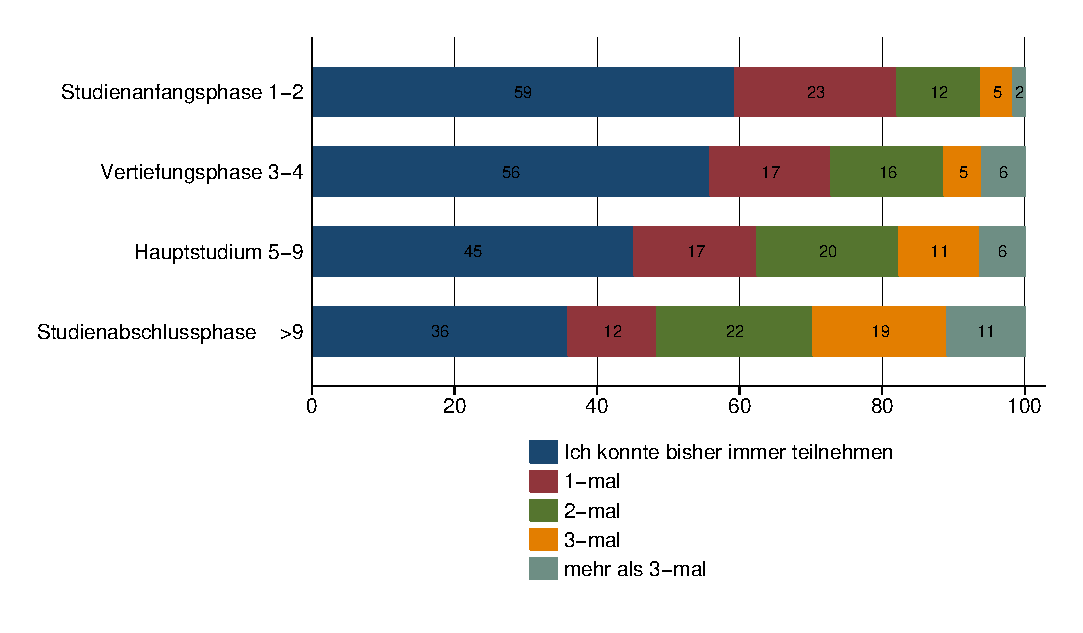
\includegraphics[
%  defaultresolution=72 !,
%  bmpsizefast=false
%]{image}
%\end{verbatim}
% \end{quote}
%
% \subsubsection{Hints}
%
% \begin{itemize}
% \item My version of \xfile{dvips.def} 1999/02/16 v3.0i defines
%       rules for the supported bitmap extensions, but does not
%       include them in the list of extensions that are tried
%       if the file name is not given with an extension.
%       In such a case, the list of extensions can be set
%       by \cs{DeclareGraphicsExtensions}, see \xpackage{grfguide}.
%       The following code just extends the list:
%       \begin{quote}
%\begin{verbatim}
%\makeatletter
%\g@addto@macro\Gin@extensions{,.bmp,.pcx,.msp}
%\makeatother
%\end{verbatim}
%       \end{quote}
% \item My version of \xfile{dvipdfm.def} 1998/11/24 vx.x misses
%       the graphics rule for PNG files. It can be added by:
%       \begin{quote}
%\begin{verbatim}
%\DeclareGraphicsRule{.png}{bmp}{.bb}{#1}
%\end{verbatim}
%       \end{quote}
%       See the previous issue to add the extension \xfile{.png} to the list
%       of extensions for package \xpackage{graphics}.
% \end{itemize}
%
% \subsubsection{Test program}
%
% There is a test program \xfile{bmpsize-test.tex}. Run it through
% \verb|latex|, \verb|pdflatex|, or \verb|pdftex|. Then given
% image files are inspected and the result is printed.
%
% \subsubsection{Interface for programmers}
%
% The macro names of the parsers are \verb|\bmpsize@read@|\meta{type}.
% Example: \cs{bmpsize@read@jpg} in case of JPEG.
%
% A parser sets the switch \cs{ifbmpsize@ok} to true, if it
% could successfully parse the image file.
% The width and height are returnd in \cs{bmpsize@width} and
% \cs{bmpsize@height}. If information about density is available,
% it is used to calculate width and height of the image, otherwise
% the values given by option \xoption{defaultresolution} is used.
% \xoption{resolution} overwrites the values in the image file.
%
% \subsection{Improved bitmap inclusion}
%
% Some drivers for package \xpackage{graphics} define the graphics
% type \xoption{bmp} for bitmap images. The code in the standard
% drivers for \xoption{dvips}, \xoption{dvipdfm}, and \xoption{dvipdfmx}
% is very basic and misses essential features of the
% package \xpackage{graphicx}. Therefore the code for bitmap
% inclusion is automatically rewritten by this package to add
% the following features:
% \begin{itemize}
% \item Support for \xoption{viewport} and \xoption{trim}.
% \item Support for \xoption{clip}.
% \item In case of \xoption{dvipdfm} and \xoption{dvipdfmx} the
%       bitmap images are reused and not included again if they
%       are used more than once.
% \end{itemize}
% However, there is a difference between \xoption{dvipdfm} and
% \xoption{dvipdfmx}, especially if images are reused. In the
% former case the reused box has width and height of 1bp, in the
% latter case its natural width. Thus the correct driver option must be given.
% \xoption{dvipdfm} and \xoption{dvipdfmx} are not equivalent.
%
% Older versions of \xoption{dvipdfmx} uses a size of 1in. However I do
% want to distinguish between versions of the same program. Therefore the
% support of these older versions has stopped with version 1.6 of this package.
% Use version dvipdfmx-20090708 or newer (some few versions before will
% probably also work, but I don't want to investigate this further).
%
% \StopEventually{
% }
%
% \section{Implementation}
%
% \subsection{Basic package \xpackage{bmpsize-base}}
%
%    Identification.
%    \begin{macrocode}
%<*base>
\ProvidesPackage{bmpsize-base}%
  [2009/09/04 v1.6 Basic part of bmpsize (HO)]%
%    \end{macrocode}
%    Modules of package \xpackage{fp} are used for calculations.
%    \begin{macrocode}
\RequirePackage{fp-basic}
\RequirePackage{fp-snap}
%    \end{macrocode}
%    Package \xpackage{fp} uses nested \cs{loop} structures.
%    That breaks with the plain-\TeX\ version of \cs{loop}.
%    Therefore we use the \LaTeX\ variant.
%    \begin{macro}{\@bmpsize@plain@loop}
%    \begin{macrocode}
\long\def\@bmpsize@plain@loop#1\repeat{%
  \def\iterate{%
    #1\relax
    \expandafter\iterate\fi
  }%
  \iterate
  \let\iterate\relax
}
%    \end{macrocode}
%    \end{macro}
%    \begin{macrocode}
\RequirePackage{pdftexcmds}[2007/11/11]
%    \end{macrocode}
%    \begin{macrocode}
\newif\ifbmpsize@ok
\let\@bmpsize@ok\bmpsize@oktrue

\newif\if@bmpsize@bigendian
\newif\if@bmpsize@absnum
\newif\if@bmpsize@user@resolution
\newif\if@bmpsize@fast
\@bmpsize@fasttrue

\def\@bmpsize@init{%
  \let\@bmpsize@org@plain@loop\loop
  \let\loop\@bmpsize@plain@loop
  \bmpsize@okfalse
  \@bmpsize@bigendiantrue
  \@bmpsize@absnumfalse
  \let\bmpsize@pixelwidth\relax
  \let\bmpsize@pixelheight\relax
  \let\bmpsize@pixelx\relax
  \let\bmpsize@pixely\relax
  \let\bmpsize@unit\relax
  \let\bmpsize@pixelxdenom\relax
  \let\bmpsize@pixelydenom\relax
  \let\bmpsize@orientation\relax
}

\def\@bmpsize@stop#1\@nil{}

\def\@bmpsize@loop#1{%
  #1%
  \@bmpsize@loop{#1}%
}
\def\@bmpsize@break#1\@bmpsize@loop#2{}

\def\@bmpsize@size#1#2#3{%
  \edef#3{\pdf@filesize{#1}}%
  \ifx#3\@empty
    \expandafter\@bmpsize@stop
  \fi
  \ifnum#3<#2\relax
    \expandafter\@bmpsize@stop
  \fi
}

\def\@bmpsize@read#1#2#3{%
  \edef\@bmpsize@buf{\pdf@filedump{#3}{#2}{#1}}%
  \edef\@bmpsize@temp{%
    \noexpand\@bmpsize@check@byte{#2}\@bmpsize@buf{}{}\noexpand\\%
  }%
  \@bmpsize@temp
}
\def\@bmpsize@fillbuf#1{%
  \ifx\@bmpsize@buf\@empty
    \expandafter\@firstofone
  \else
    \expandafter\@gobble
  \fi
  {%
    \edef\@bmpsize@buf{%
      \pdf@filedump{\bmpsize@offset}{\bmpsize@fillbuflength}{#1}%
    }%
    \ifx\@bmpsize@buf\@empty
      \expandafter\@bmpsize@stop
    \fi
    \edef\bmpsize@offset{\the\numexpr\bmpsize@offset+\bmpsize@fillbuflength}%
  }%
}
\def\bmpsize@fillbuflength{10}

\def\@bmpsize@append#1#2#3{%
  \edef#1{#2#3}%
}
\def\@bmpsize@pushback#1{%
  \edef\@bmpsize@buf{#1\@bmpsize@buf}%
}

\def\@bmpsize@iswhite#1{%
  \ifnum\pdf@strcmp{#1}{09}=\z@
  \else
    \ifnum\pdf@strcmp{#1}{0A}=\z@
    \else
      \ifnum\pdf@strcmp{#1}{0D}=\z@
      \else
        \ifnum\pdf@strcmp{#1}{20}=\z@
        \else
          1%
        \fi
      \fi
    \fi
  \fi
  \space
}
\def\@bmpsize@isdigit#1{%
  \ifnum\pdf@strcmp{#1}{30}<\z@
    1%
  \else
    \ifnum\pdf@strcmp{#1}{39}>\z@
      1%
    \fi
  \fi
  \space
}

\def\@bmpsize@check@byte#1#2#3{%
  \ifnum#1<\@ne
    \csname fi\endcsname
    \@bmpsize@cleanup@end
  \else
    \csname fi\endcsname
  \ifx!#2#3!%
    \csname fi\endcsname
    \@bmpsize@stop
  \else
    \csname fi\endcsname
    \expandafter\@bmpsize@check@byte\expandafter{\the\numexpr#1-1}%
}
\def\@bmpsize@cleanup@end#1\\{}

\def\@bmpsize@swap@maybe#1{%
  \if@bmpsize@bigendian
  \else
    \edef#1{\expandafter\@bmpsize@@swap#1\@empty\@empty\@empty\@empty}%
  \fi
}
\def\@bmpsize@@swap#1#2#3#4#5#6#7#8{%
  #7#8#5#6#3#4#1#2%
}

\def\@bmpsize@skip@one{%
  \edef\@bmpsize@buf{\expandafter\@gobbletwo\@bmpsize@buf}%
}
\def\@bmpsize@skip@two{%
  \edef\@bmpsize@buf{\expandafter\@gobblefour\@bmpsize@buf}%
}
\def\@bmpsize@skip@four{%
  \edef\@bmpsize@buf{%
    \expandafter\expandafter\expandafter\@gobblefour\expandafter
    \@gobblefour\@bmpsize@buf
  }%
}

\def\@bmpsize@grab#1#2{%
  \edef#1{\noexpand\@bmpsize@grab@byte#2=\@bmpsize@buf\noexpand\\}%
  \edef#1{#1}%
}
\def\@bmpsize@grab@byte#1=#2#3{%
  #2#3%
  \ifnum#1>\@ne
    \expandafter\@bmpsize@grab@byte\the\numexpr#1-1\expandafter=%
  \else
    \expandafter\@bmpsize@cleanup@end
  \fi
}

\def\@bmpsize@abs@maybe#1{%
  \let\@bmpsize@temp\relax
  \if@bmpsize@absnum
    \ifnum"\expandafter\@car#1\@nil>7 %
      \edef#1{\expandafter\@bmpsize@abs@byte#1\relax}%
      \ifnum\pdf@strcmp{#1}{7FFFFFFF}=\z@
        \let\@bmpsize@temp\@bmpsize@stop
      \else
        \def\@bmpsize@temp{\edef#1{\the\numexpr#1+1}}%
      \fi
    \fi
  \fi
}
\def\@bmpsize@abs@byte#1{%
  \ifx#1\relax
  \else
    \ifcase"0#1 %
      F\or E\or D\or C\or B\or A\or 9\or 8\or
      7\or 6\or 5\or 4\or 3\or 2\or 1\or 0%
    \fi
    \expandafter\@bmpsize@abs@byte
  \fi
}

\def\@bmpsize@num@one#1{%
  \@bmpsize@grab#11%
  \@bmpsize@abs@maybe#1%
  \edef#1{\number"#1}%
  \@bmpsize@temp
  \@bmpsize@skip@one
}
\def\@bmpsize@num@two#1{%
  \@bmpsize@grab#12%
  \@bmpsize@swap@maybe#1%
  \@bmpsize@abs@maybe#1%
  \edef#1{\number"#1}%
  \@bmpsize@temp
  \@bmpsize@skip@two
}
\def\@bmpsize@num@four#1{%
  \@bmpsize@grab#14%
  \@bmpsize@swap@maybe#1%
  \@bmpsize@abs@maybe#1%
  \ifnum\pdf@strcmp{#1}{7FFFFFFF}>\z@
    \expandafter\@bmpsize@stop
  \fi
  \edef#1{\number"#1}%
  \@bmpsize@temp
  \@bmpsize@skip@four
}

\def\@bmpsize@div#1#2#3{% #1 := #2/#3
  \FPdiv#1{#2}{#3}%
  \@bmpsize@beautify#1%
}
\def\@bmpsize@beautify#1{%
  \FPifint#1%
    \edef#1{\expandafter\@bmpsize@trunc#1.\@nil}%
  \else
    \edef#1{\expandafter\@bmpsize@cleanup@frac#1.\@nil}%
  \fi
}
\def\@bmpsize@trunc#1.#2\@nil{#1}
% #1 isn't an integer, thus we should have at least one
% necessary digit after the dot
\def\@bmpsize@cleanup@frac#1.#2#3.#4\@nil{%
  #1.#2%
  \ifx\\#3\\%
  \else
    \@bmpsize@cleanup@fracdigits#3000000000\@nil
  \fi
}
\def\@bmpsize@cleanup@fracdigits#1#2#3#4#5#6#7#8#9{%
  \ifcase#9 %
    \ifcase#8 %
      \ifcase#7 %
        \ifcase#6 %
          \ifcase#5 %
            \ifcase #4 %
              \ifcase #3 %
                \ifcase #2 %
                  \ifcase #1 %
                  \else
                    #1%
                  \fi
                \else
                  #1#2%
                \fi
              \else
                #1#2#3%
              \fi
            \else
              #1#2#3#4%
            \fi
          \else
            #1#2#3#4#5%
          \fi
        \else
          #1#2#3#4#5#6%
        \fi
      \else
        #1#2#3#4#5#6#7%
      \fi
    \else
      #1#2#3#4#5#6#7#8%
    \fi
  \else
    #1#2#3#4#5#6#7#8#9%
  \fi
  \@bmpsize@trunc.%
}

\def\@bmpsize@end{%
  \ifbmpsize@ok
    \ifx\bmpsize@pixelwidth\relax
      \bmpsize@okfalse
    \fi
    \ifx\bmpsize@pixelheight\relax
      \bmpsize@okfalse
    \fi
  \fi
  \ifbmpsize@ok
    \ifnum\bmpsize@pixelwidth>\z@
    \else
      \bmpsize@okfalse
    \fi
    \ifnum\bmpsize@pixelheight>\z@
    \else
      \bmpsize@okfalse
    \fi
  \fi
  \ifbmpsize@ok
    \ifcase 0%
      \ifx\bmpsize@pixelx\relax 1 \fi
      \ifx\bmpsize@pixely\relax 1 \fi
      \ifnum\bmpsize@pixelx>\z@\else 1 \fi
      \ifnum\bmpsize@pixely>\z@\else 1 \fi
      \ifx\bmpsize@pixelxdenom\relax
         \ifx\bmpsize@pixelydenom\relax\else 1 \fi
      \else
        \ifnum\bmpsize@pixelxdenom>\z@\else 1 \fi
      \fi
      \ifx\bmpsize@pixelydenom\relax
      \else
        \ifnum\bmpsize@pixelydenom>\z@\else 1 \fi
      \fi
    \else
      \let\bmpsize@pixelx\relax
      \let\bmpsize@pixely\relax
      \let\bmpsize@unit\relax
      \let\bmpsize@pixelxdenom\relax
      \let\bmpsize@pixelydenom\relax
    \fi
    \ifx\bmpsize@pixelxdenom\relax
    \else
      \@bmpsize@div\bmpsize@pixelx\bmpsize@pixelx\bmpsize@pixelxdenom
      \@bmpsize@div\bmpsize@pixely\bmpsize@pixely\bmpsize@pixelydenom
      \let\bmpsize@pixelxdenom\relax
      \let\bmpsize@pixelydenom\relax
    \fi
    \ifcase 0\ifx\bmpsize@unit\relax 1\fi
             \if@bmpsize@user@resolution 1\fi
             \relax
      \let\bmpsize@calc@unit\bmpsize@unit
      \let\bmpsize@calc@pixelx\bmpsize@pixelx
      \let\bmpsize@calc@pixely\bmpsize@pixely
    \else
      \let\bmpsize@calc@unit\bmpsize@unit@default
      \let\bmpsize@calc@pixelx\bmpsize@pixelx@default
      \let\bmpsize@calc@pixely\bmpsize@pixely@default
      \ifx\bmpsize@calc@pixely\Gin@exclamation
        \ifx\bmpsize@pixelx\relax
          \let\bmpsize@calc@pixely\bmpsize@calc@pixelx
        \else
          \FPdiv\bmpsize@calc@pixely\bmpsize@calc@pixelx\bmpsize@pixelx
          \FPmul\bmpsize@calc@pixely\bmpsize@calc@pixely\bmpsize@pixely
        \fi
      \else
        \ifx\bmpsize@calc@pixelx\Gin@exclamation
          \ifx\bmpsize@pixelx\relax
            \let\bmpsize@calc@pixelx\bmpsize@calc@pixely
          \else
            \FPdiv\bmpsize@calc@pixelx\bmpsize@calc@pixely\bmpsize@pixely
            \FPmul\bmpsize@calc@pixelx\bmpsize@calc@pixelx\bmpsize@pixelx
          \fi
        \fi
      \fi
    \fi
    \FPdiv\bmpsize@width\bmpsize@pixelwidth\bmpsize@calc@pixelx
    \FPdiv\bmpsize@height\bmpsize@pixelheight\bmpsize@calc@pixely
    % calculation of width and height in bp for package graphics
    % 1in = 72bp = 72.27pt, 72/72.27 = 8/8.03, 1pt = 65536sp
    \if@bmpsize@fast
      \edef\bmpsize@width{%
        \strip@pt\dimexpr.99626\dimexpr
        \bmpsize@width\dimexpr\bmpsize@calc@unit
      }%
      \edef\bmpsize@height{%
        \strip@pt\dimexpr.99626\dimexpr
        \bmpsize@height\dimexpr\bmpsize@calc@unit
      }%
    \else
      \edef\@bmpsize@temp{\number\dimexpr\bmpsize@calc@unit}%
      \ifnum\@bmpsize@temp>100000 %
        \FPmul\@bmpsize@temp\@bmpsize@temp{0.00001}%
        \def\@bmpsize@corr{100000}%
      \else
        \let\@bmpsize@corr\relax
      \fi
      \FPmul\bmpsize@width\bmpsize@width\@bmpsize@temp
      \FPmul\bmpsize@height\bmpsize@height\@bmpsize@temp
      \FPmul\bmpsize@width\bmpsize@width{8}%
      \FPmul\bmpsize@height\bmpsize@height{8}%
      \FPdiv\bmpsize@width\bmpsize@width{8.03}%
      \FPdiv\bmpsize@height\bmpsize@height{8.03}%
      \FPdiv\bmpsize@width\bmpsize@width{65536}%
      \FPdiv\bmpsize@height\bmpsize@height{65536}%
      \ifx\@bmpsize@corr\relax
      \else
        \FPmul\bmpsize@width\bmpsize@width\@bmpsize@corr
        \FPmul\bmpsize@height\bmpsize@height\@bmpsize@corr
      \fi
      \FPround\bmpsize@width\bmpsize@width{5}%
      \FPround\bmpsize@height\bmpsize@height{5}%
      \@bmpsize@beautify\bmpsize@width
      \@bmpsize@beautify\bmpsize@height
    \fi
  \fi
  \let\loop\@bmpsize@org@plain@loop
}
\def\bmpsize@unit@default{72.27pt}% more accurate than 1in
\def\bmpsize@pixelx@default{72}
\let\bmpsize@pixely@default\Gin@exclamation

\def\bmpsize@types{png,jpg,bmp,gif,tiff,pnm,pam,xpm,tga,pcx,msp,sgi}
%</base>
%    \end{macrocode}
%
% \subsection{Bitmap formats}
%
% \subsubsection{png}
%
%\iffalse
%<*ignore>
%\fi
%\begin{verbatim}
%begin png
%big-endian
%
%read 24 0
%grab 8        -> $temp
%check streq $temp [0x89 "PNG" 0x0D 0x0A 0x1A 0x0A]
%num 4         -> $length
%grab 4        -> $temp
%check streq $temp ["IHDR"]
%num 4         -> $pixelwidth
%num 4         -> $pixelheight
%ok
%assign numexpr(20 + $length) -> $offset
%loop
%  read 8 $offset
%  num 4       -> $length
%  grab 4      -> $temp
%  if streq $temp ["IDAT"]
%    stop
%  fi
%  if streq $temp ["pHYs"]
%    read 9 numexpr($offset + 8)
%    num 4     -> $pixelx
%    num 4     -> $pixely
%    grab 1     -> $temp
%    if numeq $temp 1
%      assign {100cm} -> $unit
%    fi
%    stop
%  fi
%  assign numexpr($offset + 12 + $length) -> $offset
%repeat
%end
%\end{verbatim}
%\iffalse
%</ignore>
%\fi
%    \begin{macro}{\bmpsize@read@png}
%    \begin{macrocode}
%<*base>
\def\bmpsize@read@png#1{%
  \@bmpsize@init
  \@bmpsize@bigendiantrue
  \@bmpsize@read{#1}{24}{0}%
  \@bmpsize@grab\bmpsize@temp{8}%
  \@bmpsize@skip@four
  \@bmpsize@skip@four
  \ifnum\pdf@strcmp{\bmpsize@temp}{89504E470D0A1A0A}=\z@
  \else
    \expandafter\@bmpsize@stop
  \fi
  \@bmpsize@num@four\bmpsize@length
  \@bmpsize@grab\bmpsize@temp{4}%
  \@bmpsize@skip@four
  \ifnum\pdf@strcmp{\bmpsize@temp}{49484452}=\z@
  \else
    \expandafter\@bmpsize@stop
  \fi
  \@bmpsize@num@four\bmpsize@pixelwidth
  \@bmpsize@num@four\bmpsize@pixelheight
  \@bmpsize@ok
  \edef\bmpsize@offset{\the\numexpr20+\bmpsize@length}%
  \@bmpsize@loop{%
    \@bmpsize@read{#1}{8}{\bmpsize@offset}%
    \@bmpsize@num@four\bmpsize@length
    \@bmpsize@grab\bmpsize@temp{4}%
    \@bmpsize@skip@four
    \ifnum\pdf@strcmp{\bmpsize@temp}{49444154}=\z@
      \expandafter\@firstofone
    \else
      \expandafter\@gobble
    \fi
    {%
      \@bmpsize@stop
    }%
    \ifnum\pdf@strcmp{\bmpsize@temp}{70485973}=\z@
      \expandafter\@firstofone
    \else
      \expandafter\@gobble
    \fi
    {%
      \@bmpsize@read{#1}{9}{\numexpr\bmpsize@offset+8\relax}%
      \@bmpsize@num@four\bmpsize@pixelx
      \@bmpsize@num@four\bmpsize@pixely
      \@bmpsize@grab\bmpsize@temp{1}%
      \@bmpsize@skip@one
      \ifnum\bmpsize@temp=1\relax
        \expandafter\@firstofone
      \else
        \expandafter\@gobble
      \fi
      {%
        \def\bmpsize@unit{100cm}%
      }%
      \@bmpsize@stop
    }%
    \edef\bmpsize@offset{\the\numexpr\bmpsize@offset+12+\bmpsize@length}%
  }%
  \@bmpsize@stop
  \@nil
  \@bmpsize@end
}%
%</base>
%    \end{macrocode}
%    \end{macro}
%
% \subsubsection{jpg}
%
%\iffalse
%<*ignore>
%\fi
%\begin{verbatim}
%begin jpg
%
%read 3 0
%grab 3      -> $temp % SOI and 0xFF
%check streq $temp [0xFF 0xD8 0xFF]
%assign {2} -> $offset
%assign {0} -> $exifdensity
%loop
%  read 4 $offset
%  grab 1    -> $temp
%  check streq $temp [0xFF]
%  num 1    -> $temp
%  if numeq $temp 0xDA % SOS
%    stop
%  fi
%  % look for JFIF APP0 segment
%  if numeq $temp 0xE0 % APP0
%    num 2       -> $length
%    if numeq $exifdensity 0
%      if numge $length 16 % a JFIF segment has 16 bytes at least
%        read 12 numexpr($offset + 4)
%        grab 5      -> $temp % identifier
%        if streq $temp ["JFIF" 0x0]
%          check numge $length 16
%          skip 2 % version
%          num 1       -> $temp % units
%          if numeq $temp 1
%            assign {72.27pt} -> $unit
%          else
%            if numeq $temp 2
%              assign {1cm} -> $unit
%            fi
%          fi
%          num 2    -> $pixelx
%          num 2    -> $pixely
%        fi
%      fi
%    fi
%  else
%    if numeq $temp 0xE1 % APP1
%      % look for Exif APP1 segment
%      num 2 -> $length
%      if numge $length 20 % identifier (6) + Tiff header (8) + first IFD (>=6)
%        read 20 numexpr($offset + 4)
%        grab 6 -> $temp
%        if streq $temp ["Exif" 0x0 0x0]
%          assign numexpr($offset + 10) -> $exifoffset
%          % read TIFF header
%          grab 2 -> $temp
%          if streq $temp ["II"]
%            little-endian
%          else
%            check streq $temp ["MM"]
%            % big-endian
%          fi
%          num 2 -> $temp
%          check numeq $temp 42
%          num 4 -> $temp % offset of first IFD
%          check numgt $temp 0
%          % read first IFD
%          assign numexpr($temp + $exifoffset) -> $off
%          read 2 $off
%          num 2 -> $entries
%          assign numexpr($off + 2) -> $off
%          loop
%            if numeq $entries 0
%              break
%            fi
%            assign numexpr($entries - 1) -> $entries
%            % entry format:
%            % 2 tag
%            % 2 field type
%            % 4 count
%            % 4 value/offset
%            read 12 $off
%            assign numexpr($off + 12) -> $off
%            num 2 -> $tag
%            if numeq $tag 296 % ResolutionUnit
%              skip 6 % type: 3 (short), count: 1
%              num 2 -> $temp
%              ifcase $temp
%              or % 1
%                clear $unit
%              or % 2
%                assign {72.27pt} -> $unit
%              or % 3
%                assign {1cm} -> $unit
%              else
%                clear $unit % unknown
%              fi
%              ifcase $temp
%              or % 1
%              or % 2
%                assign {1} -> $exifdensity
%              or % 3
%                assign {1} -> $exifdensity
%              else
%                assign $exifdensity -> $exifdensity
%              fi
%            fi
%            % 256 ImageWidth (use width of JPG part)
%            % 257 ImageHeight (use height of JPG part)
%            if numeq $tag 274 % Orientation
%              skip 6 % type: 3 (short), count: 1
%              num 2 -> $temp
%              if numge $temp 0 
%                if numle $temp 8
%                  assign $temp -> $orientation
%                fi
%              fi
%            fi
%            if numeq $tag 282 % XResolution
%              skip 6
%              num 4 -> $temp
%              read 8 numexpr($temp + $exifoffset)
%              num 4 -> $pixelx
%              num 4 -> $temp
%              if numeq $temp 1
%              else
%                assign numexpr($temp) -> $pixelxdenom
%                % div $pixelx $temp -> $pixelx
%              fi
%            fi
%            if numeq $tag 283 % YResolution
%              skip 6
%              num 4 -> $temp
%              read 8 numexpr($temp + $exifoffset)
%              num 4 -> $pixely
%              num 4 -> $temp
%              if numeq $temp 1
%              else
%                assign numexpr($temp) -> $pixelydenom
%                % div $pixely $temp -> $pixely
%              fi
%            fi
%          repeat
%          big-endian
%        fi
%      fi
%    else
%      assign numexpr($temp - 0xC0) -> $temp
%      ifcase $temp % SOF_0
%      or % SOF_1
%      or % SOF_2
%      or % SOF_3
%      or % DHT
%        assign {-1} -> $temp
%      or % SOF_5
%      or % SOF_6
%      or % SOF_7
%      or % JPG
%        assign {-1} -> $temp
%      or % SOF_9
%      or % SOF_10
%      or % SOF_11
%      or % DAC
%        assign {-1} -> $temp
%      or % SOF_13
%      or % SOF_14
%      or % SOF_15
%      else
%        assign {-1} -> $temp
%      fi
%      if numeq $temp -1
%      else
%        read 4 numexpr($offset + 5)
%        num 2  -> $pixelheight
%        num 2  -> $pixelwidth
%        if numeq $pixelheight 0
%          clear $pixelheight
%          stop
%        fi
%        ok
%        stop
%      fi
%      num 2 -> $length
%    fi
%  fi
%  assign numexpr($offset + $length + 2) -> $offset
%repeat
%end
%\end{verbatim}
%\iffalse
%</ignore>
%\fi
%    \begin{macro}{\bmpsize@read@jpg}
%    \begin{macrocode}
%<*base>
\def\bmpsize@read@jpg#1{%
  \@bmpsize@init
  \@bmpsize@read{#1}{3}{0}%
  \@bmpsize@grab\bmpsize@temp{3}%
  \@bmpsize@skip@two
  \@bmpsize@skip@one
  \ifnum\pdf@strcmp{\bmpsize@temp}{FFD8FF}=\z@
  \else
    \expandafter\@bmpsize@stop
  \fi
  \def\bmpsize@offset{2}%
  \def\bmpsize@exifdensity{0}%
  \@bmpsize@loop{%
    \@bmpsize@read{#1}{4}{\bmpsize@offset}%
    \@bmpsize@grab\bmpsize@temp{1}%
    \@bmpsize@skip@one
    \ifnum\pdf@strcmp{\bmpsize@temp}{FF}=\z@
    \else
      \expandafter\@bmpsize@stop
    \fi
    \@bmpsize@num@one\bmpsize@temp
    \ifnum\bmpsize@temp=218\relax
      \expandafter\@firstofone
    \else
      \expandafter\@gobble
    \fi
    {%
      \@bmpsize@stop
    }%
    \ifnum\bmpsize@temp=224\relax
      \expandafter\@firstoftwo
    \else
      \expandafter\@secondoftwo
    \fi
    {%
      \@bmpsize@num@two\bmpsize@length
      \ifnum\bmpsize@exifdensity=0\relax
        \expandafter\@firstofone
      \else
        \expandafter\@gobble
      \fi
      {%
        \unless\ifnum\bmpsize@length<16\relax
          \expandafter\@firstofone
        \else
          \expandafter\@gobble
        \fi
        {%
          \@bmpsize@read{#1}{12}{\numexpr\bmpsize@offset+4\relax}%
          \@bmpsize@grab\bmpsize@temp{5}%
          \@bmpsize@skip@four
          \@bmpsize@skip@one
          \ifnum\pdf@strcmp{\bmpsize@temp}{4A46494600}=\z@
            \expandafter\@firstofone
          \else
            \expandafter\@gobble
          \fi
          {%
            \ifnum\bmpsize@length<16\relax
              \expandafter\@bmpsize@stop
            \fi
            \@bmpsize@skip@two
            \@bmpsize@num@one\bmpsize@temp
            \ifnum\bmpsize@temp=1\relax
              \expandafter\@firstoftwo
            \else
              \expandafter\@secondoftwo
            \fi
            {%
              \def\bmpsize@unit{72.27pt}%
            }{%
              \ifnum\bmpsize@temp=2\relax
                \expandafter\@firstofone
              \else
                \expandafter\@gobble
              \fi
              {%
                \def\bmpsize@unit{1cm}%
              }%
            }%
            \@bmpsize@num@two\bmpsize@pixelx
            \@bmpsize@num@two\bmpsize@pixely
          }%
        }%
      }%
    }{%
      \ifnum\bmpsize@temp=225\relax
        \expandafter\@firstoftwo
      \else
        \expandafter\@secondoftwo
      \fi
      {%
        \@bmpsize@num@two\bmpsize@length
        \unless\ifnum\bmpsize@length<20\relax
          \expandafter\@firstofone
        \else
          \expandafter\@gobble
        \fi
        {%
          \@bmpsize@read{#1}{20}{\numexpr\bmpsize@offset+4\relax}%
          \@bmpsize@grab\bmpsize@temp{6}%
          \@bmpsize@skip@four
          \@bmpsize@skip@two
          \ifnum\pdf@strcmp{\bmpsize@temp}{457869660000}=\z@
            \expandafter\@firstofone
          \else
            \expandafter\@gobble
          \fi
          {%
            \edef\bmpsize@exifoffset{\the\numexpr\bmpsize@offset+10}%
            \@bmpsize@grab\bmpsize@temp{2}%
            \@bmpsize@skip@two
            \ifnum\pdf@strcmp{\bmpsize@temp}{4949}=\z@
              \expandafter\@firstoftwo
            \else
              \expandafter\@secondoftwo
            \fi
            {%
              \@bmpsize@bigendianfalse
            }{%
              \ifnum\pdf@strcmp{\bmpsize@temp}{4D4D}=\z@
              \else
                \expandafter\@bmpsize@stop
              \fi
            }%
            \@bmpsize@num@two\bmpsize@temp
            \ifnum\bmpsize@temp=42\relax
            \else
              \expandafter\@bmpsize@stop
            \fi
            \@bmpsize@num@four\bmpsize@temp
            \ifnum\bmpsize@temp>0\relax
            \else
              \expandafter\@bmpsize@stop
            \fi
            \edef\bmpsize@off{\the\numexpr\bmpsize@temp+\bmpsize@exifoffset}%
            \@bmpsize@read{#1}{2}{\bmpsize@off}%
            \@bmpsize@num@two\bmpsize@entries
            \edef\bmpsize@off{\the\numexpr\bmpsize@off+2}%
            \@bmpsize@loop{%
              \ifnum\bmpsize@entries=0\relax
                \expandafter\@firstofone
              \else
                \expandafter\@gobble
              \fi
              {%
                \@bmpsize@break
              }%
              \edef\bmpsize@entries{\the\numexpr\bmpsize@entries-1}%
              \@bmpsize@read{#1}{12}{\bmpsize@off}%
              \edef\bmpsize@off{\the\numexpr\bmpsize@off+12}%
              \@bmpsize@num@two\bmpsize@tag
              \ifnum\bmpsize@tag=296\relax
                \expandafter\@firstofone
              \else
                \expandafter\@gobble
              \fi
              {%
                \@bmpsize@skip@four
                \@bmpsize@skip@two
                \@bmpsize@num@two\bmpsize@temp
                \ifcase\bmpsize@temp\relax
                \or
                  \let\bmpsize@unit\relax
                \or
                  \def\bmpsize@unit{72.27pt}%
                \or
                  \def\bmpsize@unit{1cm}%
                \else
                  \let\bmpsize@unit\relax
                \fi
                \ifcase\bmpsize@temp\relax
                \or
                \or
                  \def\bmpsize@exifdensity{1}%
                \or
                  \def\bmpsize@exifdensity{1}%
                \else
                  \let\bmpsize@exifdensity\bmpsize@exifdensity
                \fi
              }%
              \ifnum\bmpsize@tag=274\relax
                \expandafter\@firstofone
              \else
                \expandafter\@gobble
              \fi
              {%
                \@bmpsize@skip@four
                \@bmpsize@skip@two
                \@bmpsize@num@two\bmpsize@temp
                \unless\ifnum\bmpsize@temp<0\relax
                  \expandafter\@firstofone
                \else
                  \expandafter\@gobble
                \fi
                {%
                  \unless\ifnum\bmpsize@temp>8\relax
                    \expandafter\@firstofone
                  \else
                    \expandafter\@gobble
                  \fi
                  {%
                    \let\bmpsize@orientation\bmpsize@temp
                  }%
                }%
              }%
              \ifnum\bmpsize@tag=282\relax
                \expandafter\@firstofone
              \else
                \expandafter\@gobble
              \fi
              {%
                \@bmpsize@skip@four
                \@bmpsize@skip@two
                \@bmpsize@num@four\bmpsize@temp
                \@bmpsize@read{#1}{8}{\numexpr\bmpsize@temp+\bmpsize@exifoffset\relax}%
                \@bmpsize@num@four\bmpsize@pixelx
                \@bmpsize@num@four\bmpsize@temp
                \ifnum\bmpsize@temp=1\relax
                  \expandafter\@gobble
                \else
                  \expandafter\@firstofone
                \fi
                {%
                  \edef\bmpsize@pixelxdenom{\the\numexpr\bmpsize@temp}%
                }%
              }%
              \ifnum\bmpsize@tag=283\relax
                \expandafter\@firstofone
              \else
                \expandafter\@gobble
              \fi
              {%
                \@bmpsize@skip@four
                \@bmpsize@skip@two
                \@bmpsize@num@four\bmpsize@temp
                \@bmpsize@read{#1}{8}{\numexpr\bmpsize@temp+\bmpsize@exifoffset\relax}%
                \@bmpsize@num@four\bmpsize@pixely
                \@bmpsize@num@four\bmpsize@temp
                \ifnum\bmpsize@temp=1\relax
                  \expandafter\@gobble
                \else
                  \expandafter\@firstofone
                \fi
                {%
                  \edef\bmpsize@pixelydenom{\the\numexpr\bmpsize@temp}%
                }%
              }%
            }%
            \@bmpsize@bigendiantrue
          }%
        }%
      }{%
        \edef\bmpsize@temp{\the\numexpr\bmpsize@temp-192}%
        \ifcase\bmpsize@temp\relax
        \or
        \or
        \or
        \or
          \def\bmpsize@temp{-1}%
        \or
        \or
        \or
        \or
          \def\bmpsize@temp{-1}%
        \or
        \or
        \or
        \or
          \def\bmpsize@temp{-1}%
        \or
        \or
        \or
        \else
          \def\bmpsize@temp{-1}%
        \fi
        \ifnum\bmpsize@temp=-1\relax
          \expandafter\@gobble
        \else
          \expandafter\@firstofone
        \fi
        {%
          \@bmpsize@read{#1}{4}{\numexpr\bmpsize@offset+5\relax}%
          \@bmpsize@num@two\bmpsize@pixelheight
          \@bmpsize@num@two\bmpsize@pixelwidth
          \ifnum\bmpsize@pixelheight=0\relax
            \expandafter\@firstofone
          \else
            \expandafter\@gobble
          \fi
          {%
            \let\bmpsize@pixelheight\relax
            \@bmpsize@stop
          }%
          \@bmpsize@ok
          \@bmpsize@stop
        }%
        \@bmpsize@num@two\bmpsize@length
      }%
    }%
    \edef\bmpsize@offset{\the\numexpr\bmpsize@offset+\bmpsize@length+2}%
  }%
  \@bmpsize@stop
  \@nil
  \@bmpsize@end
}%
%</base>
%    \end{macrocode}
%    \end{macro}
%
% \subsubsection{bmp}
%
%\iffalse
%<*ignore>
%\fi
%\begin{verbatim}
%begin bmp
%little-endian
%
%read 26 0
%grab 2 -> $temp
%check streq $temp ["BM"]
%skip 12
%% header size is 4 bytes in V3+, unknown for V1, V2,
%% known header sizes fit in 2 bytes
%num 2   -> $temp
%if numeq $temp 12 % V1
%  skip 2
%  num 2 -> $pixelwidth
%  num 2 -> $pixelheight
%  % no resolution entries
%  ok
%  stop
%fi
%if numeq $temp 64 % V2
%  skip 2
%  num 2 -> $pixelwidth
%  num 2 -> $pixelheight
%  % missing specification for resolution
%  ok
%  stop
%fi
%% V3, V4, V5
%skip 2
%num 4 -> $pixelwidth
%absnum 4 -> $pixelheight
%ok
%read 8 38
%num 4 -> $pixelx
%num 4 -> $pixely
%assign {100cm} -> $unit
%end
%\end{verbatim}
%\iffalse
%</ignore>
%\fi
%    \begin{macro}{\bmpsize@read@bmp}
%    \begin{macrocode}
%<*base>
\def\bmpsize@read@bmp#1{%
  \@bmpsize@init
  \@bmpsize@bigendianfalse
  \@bmpsize@read{#1}{26}{0}%
  \@bmpsize@grab\bmpsize@temp{2}%
  \@bmpsize@skip@two
  \ifnum\pdf@strcmp{\bmpsize@temp}{424D}=\z@
  \else
    \expandafter\@bmpsize@stop
  \fi
  \@bmpsize@skip@four
  \@bmpsize@skip@four
  \@bmpsize@skip@four
  \@bmpsize@num@two\bmpsize@temp
  \ifnum\bmpsize@temp=12\relax
    \expandafter\@firstofone
  \else
    \expandafter\@gobble
  \fi
  {%
    \@bmpsize@skip@two
    \@bmpsize@num@two\bmpsize@pixelwidth
    \@bmpsize@num@two\bmpsize@pixelheight
    \@bmpsize@ok
    \@bmpsize@stop
  }%
  \ifnum\bmpsize@temp=64\relax
    \expandafter\@firstofone
  \else
    \expandafter\@gobble
  \fi
  {%
    \@bmpsize@skip@two
    \@bmpsize@num@two\bmpsize@pixelwidth
    \@bmpsize@num@two\bmpsize@pixelheight
    \@bmpsize@ok
    \@bmpsize@stop
  }%
  \@bmpsize@skip@two
  \@bmpsize@num@four\bmpsize@pixelwidth
  \@bmpsize@absnumtrue
  \@bmpsize@num@four\bmpsize@pixelheight
  \@bmpsize@absnumfalse
  \@bmpsize@ok
  \@bmpsize@read{#1}{8}{38}%
  \@bmpsize@num@four\bmpsize@pixelx
  \@bmpsize@num@four\bmpsize@pixely
  \def\bmpsize@unit{100cm}%
  \@bmpsize@stop
  \@nil
  \@bmpsize@end
}%
%</base>
%    \end{macrocode}
%    \end{macro}
%
% \subsubsection{gif}
%
%\iffalse
%<*ignore>
%\fi
%\begin{verbatim}
%begin gif
%little-endian
%
%% Header
%read 13 0
%grab 3      -> $temp
%check streq $temp ["GIF"]
%skip 3      % version
%
%% Logical Screen Descriptor
%num 2       -> $pixelwidth
%num 2       -> $pixelheight
%skip 2
%num 1       -> $temp % Pixel Aspect Ratio
%if numeq $temp 0
%else
%  assign numexpr($temp + 15) -> $pixelx
%  assign {64}     -> $pixely
%fi
%ok
%end
%\end{verbatim}
%\iffalse
%</ignore>
%\fi
%    \begin{macro}{\bmpsize@read@gif}
%    \begin{macrocode}
%<*base>
\def\bmpsize@read@gif#1{%
  \@bmpsize@init
  \@bmpsize@bigendianfalse
  \@bmpsize@read{#1}{13}{0}%
  \@bmpsize@grab\bmpsize@temp{3}%
  \@bmpsize@skip@two
  \@bmpsize@skip@one
  \ifnum\pdf@strcmp{\bmpsize@temp}{474946}=\z@
  \else
    \expandafter\@bmpsize@stop
  \fi
  \@bmpsize@skip@two
  \@bmpsize@skip@one
  \@bmpsize@num@two\bmpsize@pixelwidth
  \@bmpsize@num@two\bmpsize@pixelheight
  \@bmpsize@skip@two
  \@bmpsize@num@one\bmpsize@temp
  \ifnum\bmpsize@temp=0\relax
    \expandafter\@gobble
  \else
    \expandafter\@firstofone
  \fi
  {%
    \edef\bmpsize@pixelx{\the\numexpr\bmpsize@temp+15}%
    \def\bmpsize@pixely{64}%
  }%
  \@bmpsize@ok
  \@bmpsize@stop
  \@nil
  \@bmpsize@end
}%
%</base>
%    \end{macrocode}
%    \end{macro}
%
% \subsubsection{tiff}
%
%\iffalse
%<*ignore>
%\fi
%\begin{verbatim}
%begin tiff
%% defaults
%assign {72.27pt} -> $unit
%
%% Image File Header
%read 8 0
%grab 2 -> $temp
%if streq $temp ["II"]
%  little-endian
%else
%  check streq $temp ["MM"]
%  big-endian
%fi
%num 2 -> $temp
%check numeq $temp 42
%num 4 -> $offset % first IFD (Image File Directory)
%
%% First IFD
%read 2 $offset
%assign numexpr($offset + 2) -> $offset
%num 2 -> $entries
%ok % must rely on checks at the end
%loop
%  if numeq $entries 0
%    stop
%  fi
%  assign numexpr($entries - 1) -> $entries
%  % entry format:
%  % 2 tag
%  % 2 field type
%  % 4 count
%  % 4 value/offset
%  read 12 $offset
%  assign numexpr($offset + 12) -> $offset
%  num 2 -> $tag % tag
%  if numeq $temp 296 % ResolutionUnit
%    skip 6 % type: 3 (short), count: 1
%    num 2 -> $temp
%    ifcase $temp
%    or % 1
%      clear $unit
%    or % 2
%      assign {72.27pt} -> $unit
%    or % 3
%      assign {1cm} -> $unit
%    else
%      clear $unit
%    fi
%  fi
%  if numeq $tag 256 % ImageWidth
%    skip 6
%    num 4 -> $pixelwidth
%  fi
%  if numeq $tag 257 % ImageLength
%    skip 6
%    num 4 -> $pixelheight
%  fi
%  if numeq $tag 282 % XResolution
%    skip 6
%    num 4 -> $temp
%    read 8 $temp
%    num 4 -> $pixelx
%    num 4 -> $temp
%    if numeq $temp 1
%    else
%      assign numexpr($temp) -> $pixelxdenom
%      % div $pixelx $temp -> $pixelx
%    fi
%  fi
%  if numeq $tag 283 % YResolution
%    skip 6
%    num 4 -> $temp
%    read 8 $temp
%    num 4 -> $pixely
%    num 4 -> $temp
%    if numeq $temp 1
%    else
%      assign numexpr($temp) -> $pixelydenom
%      % div $pixely $temp -> $pixely
%    fi
%  fi
%repeat
%end
%\end{verbatim}
%\iffalse
%</ignore>
%\fi
%    \begin{macro}{\bmpsize@read@tiff}
%    \begin{macrocode}
%<*base>
\def\bmpsize@read@tiff#1{%
  \@bmpsize@init
  \def\bmpsize@unit{72.27pt}%
  \@bmpsize@read{#1}{8}{0}%
  \@bmpsize@grab\bmpsize@temp{2}%
  \@bmpsize@skip@two
  \ifnum\pdf@strcmp{\bmpsize@temp}{4949}=\z@
    \expandafter\@firstoftwo
  \else
    \expandafter\@secondoftwo
  \fi
  {%
    \@bmpsize@bigendianfalse
  }{%
    \ifnum\pdf@strcmp{\bmpsize@temp}{4D4D}=\z@
    \else
      \expandafter\@bmpsize@stop
    \fi
    \@bmpsize@bigendiantrue
  }%
  \@bmpsize@num@two\bmpsize@temp
  \ifnum\bmpsize@temp=42\relax
  \else
    \expandafter\@bmpsize@stop
  \fi
  \@bmpsize@num@four\bmpsize@offset
  \@bmpsize@read{#1}{2}{\bmpsize@offset}%
  \edef\bmpsize@offset{\the\numexpr\bmpsize@offset+2}%
  \@bmpsize@num@two\bmpsize@entries
  \@bmpsize@ok
  \@bmpsize@loop{%
    \ifnum\bmpsize@entries=0\relax
      \expandafter\@firstofone
    \else
      \expandafter\@gobble
    \fi
    {%
      \@bmpsize@stop
    }%
    \edef\bmpsize@entries{\the\numexpr\bmpsize@entries-1}%
    \@bmpsize@read{#1}{12}{\bmpsize@offset}%
    \edef\bmpsize@offset{\the\numexpr\bmpsize@offset+12}%
    \@bmpsize@num@two\bmpsize@tag
    \ifnum\bmpsize@temp=296\relax
      \expandafter\@firstofone
    \else
      \expandafter\@gobble
    \fi
    {%
      \@bmpsize@skip@four
      \@bmpsize@skip@two
      \@bmpsize@num@two\bmpsize@temp
      \ifcase\bmpsize@temp\relax
      \or
        \let\bmpsize@unit\relax
      \or
        \def\bmpsize@unit{72.27pt}%
      \or
        \def\bmpsize@unit{1cm}%
      \else
        \let\bmpsize@unit\relax
      \fi
    }%
    \ifnum\bmpsize@tag=256\relax
      \expandafter\@firstofone
    \else
      \expandafter\@gobble
    \fi
    {%
      \@bmpsize@skip@four
      \@bmpsize@skip@two
      \@bmpsize@num@four\bmpsize@pixelwidth
    }%
    \ifnum\bmpsize@tag=257\relax
      \expandafter\@firstofone
    \else
      \expandafter\@gobble
    \fi
    {%
      \@bmpsize@skip@four
      \@bmpsize@skip@two
      \@bmpsize@num@four\bmpsize@pixelheight
    }%
    \ifnum\bmpsize@tag=282\relax
      \expandafter\@firstofone
    \else
      \expandafter\@gobble
    \fi
    {%
      \@bmpsize@skip@four
      \@bmpsize@skip@two
      \@bmpsize@num@four\bmpsize@temp
      \@bmpsize@read{#1}{8}{\bmpsize@temp}%
      \@bmpsize@num@four\bmpsize@pixelx
      \@bmpsize@num@four\bmpsize@temp
      \ifnum\bmpsize@temp=1\relax
        \expandafter\@gobble
      \else
        \expandafter\@firstofone
      \fi
      {%
        \edef\bmpsize@pixelxdenom{\the\numexpr\bmpsize@temp}%
      }%
    }%
    \ifnum\bmpsize@tag=283\relax
      \expandafter\@firstofone
    \else
      \expandafter\@gobble
    \fi
    {%
      \@bmpsize@skip@four
      \@bmpsize@skip@two
      \@bmpsize@num@four\bmpsize@temp
      \@bmpsize@read{#1}{8}{\bmpsize@temp}%
      \@bmpsize@num@four\bmpsize@pixely
      \@bmpsize@num@four\bmpsize@temp
      \ifnum\bmpsize@temp=1\relax
        \expandafter\@gobble
      \else
        \expandafter\@firstofone
      \fi
      {%
        \edef\bmpsize@pixelydenom{\the\numexpr\bmpsize@temp}%
      }%
    }%
  }%
  \@bmpsize@stop
  \@nil
  \@bmpsize@end
}%
%</base>
%    \end{macrocode}
%    \end{macro}
%
% \subsubsection{pnm}
%
%\iffalse
%<*ignore>
%\fi
%\begin{verbatim}
%begin pnm
%assign {0} -> $offset
%read 3 $offset
%assign {3} -> $offset
%grab 1 -> $temp
%check streq $temp ["P"]
%grab 1 -> $temp
%check strge $temp ["1"]
%check strle $temp ["6"]
%% ensure one white space
%grab 1 -> $temp
%if iswhite $temp
%else
%  stop
%fi
%loop
%  % skip white space
%  fillbuf
%  grab 1 -> $temp
%  if iswhite $temp
%  else
%    if streq $temp ["#"]
%      % ignore comments
%      loop
%        fillbuf
%        grab 1 -> $temp
%        if streq $temp [0x0A]
%          break
%        else
%          if streq $temp [0x0D]
%            break
%          fi
%        fi
%      repeat
%    else
%      pushback $temp
%      break
%    fi
%  fi
%repeat
%assign {} -> $tempnum
%loop
%  fillbuf
%  grab 1 -> $temp
%  if isdigit $temp
%    append $tempnum $temp -> $tempnum
%  else
%    if iswhite $temp
%      break
%    else
%      stop
%    fi
%  fi
%repeat
%assign unescapehex($tempnum) -> $pixelwidth
%loop
%  fillbuf
%  grab 1 -> $temp
%  if iswhite $temp
%  else
%    pushback $temp
%    break
%  fi
%repeat
%assign {} -> $tempnum
%loop
%  fillbuf
%  grab 1 -> $temp
%  if isdigit $temp
%    append $tempnum $temp -> $tempnum
%  else
%    if iswhite $temp
%      break
%    else
%      stop
%    fi
%  fi
%repeat
%assign unescapehex($tempnum) -> $pixelheight
%ok
%end
%\end{verbatim}
%\iffalse
%</ignore>
%\fi
%    \begin{macro}{\bmpsize@read@pnm}
%    \begin{macrocode}
%<*base>
\def\bmpsize@read@pnm#1{%
  \@bmpsize@init
  \def\bmpsize@offset{0}%
  \@bmpsize@read{#1}{3}{\bmpsize@offset}%
  \def\bmpsize@offset{3}%
  \@bmpsize@grab\bmpsize@temp{1}%
  \@bmpsize@skip@one
  \ifnum\pdf@strcmp{\bmpsize@temp}{50}=\z@
  \else
    \expandafter\@bmpsize@stop
  \fi
  \@bmpsize@grab\bmpsize@temp{1}%
  \@bmpsize@skip@one
  \ifnum\pdf@strcmp{\bmpsize@temp}{31}<\z@
    \expandafter\@bmpsize@stop
  \fi
  \ifnum\pdf@strcmp{\bmpsize@temp}{36}>\z@
    \expandafter\@bmpsize@stop
  \fi
  \@bmpsize@grab\bmpsize@temp{1}%
  \@bmpsize@skip@one
  \ifcase 0\@bmpsize@iswhite\bmpsize@temp
    \expandafter\@gobble
  \else
    \expandafter\@firstofone
  \fi
  {%
    \@bmpsize@stop
  }%
  \@bmpsize@loop{%
    \@bmpsize@fillbuf{#1}%
    \@bmpsize@grab\bmpsize@temp{1}%
    \@bmpsize@skip@one
    \ifcase 0\@bmpsize@iswhite\bmpsize@temp
      \expandafter\@gobble
    \else
      \expandafter\@firstofone
    \fi
    {%
      \ifnum\pdf@strcmp{\bmpsize@temp}{23}=\z@
        \expandafter\@firstoftwo
      \else
        \expandafter\@secondoftwo
      \fi
      {%
        \@bmpsize@loop{%
          \@bmpsize@fillbuf{#1}%
          \@bmpsize@grab\bmpsize@temp{1}%
          \@bmpsize@skip@one
          \ifnum\pdf@strcmp{\bmpsize@temp}{0A}=\z@
            \expandafter\@firstoftwo
          \else
            \expandafter\@secondoftwo
          \fi
          {%
            \@bmpsize@break
          }{%
            \ifnum\pdf@strcmp{\bmpsize@temp}{0D}=\z@
              \expandafter\@firstofone
            \else
              \expandafter\@gobble
            \fi
            {%
              \@bmpsize@break
            }%
          }%
        }%
      }{%
        \@bmpsize@pushback\bmpsize@temp
        \@bmpsize@break
      }%
    }%
  }%
  \def\bmpsize@tempnum{}%
  \@bmpsize@loop{%
    \@bmpsize@fillbuf{#1}%
    \@bmpsize@grab\bmpsize@temp{1}%
    \@bmpsize@skip@one
    \ifcase 0\@bmpsize@isdigit\bmpsize@temp
      \expandafter\@firstoftwo
    \else
      \expandafter\@secondoftwo
    \fi
    {%
      \@bmpsize@append\bmpsize@tempnum\bmpsize@tempnum\bmpsize@temp
    }{%
      \ifcase 0\@bmpsize@iswhite\bmpsize@temp
        \expandafter\@firstoftwo
      \else
        \expandafter\@secondoftwo
      \fi
      {%
        \@bmpsize@break
      }{%
        \@bmpsize@stop
      }%
    }%
  }%
  \edef\bmpsize@pixelwidth{\pdf@unescapehex{\bmpsize@tempnum}}%
  \@bmpsize@loop{%
    \@bmpsize@fillbuf{#1}%
    \@bmpsize@grab\bmpsize@temp{1}%
    \@bmpsize@skip@one
    \ifcase 0\@bmpsize@iswhite\bmpsize@temp
      \expandafter\@gobble
    \else
      \expandafter\@firstofone
    \fi
    {%
      \@bmpsize@pushback\bmpsize@temp
      \@bmpsize@break
    }%
  }%
  \def\bmpsize@tempnum{}%
  \@bmpsize@loop{%
    \@bmpsize@fillbuf{#1}%
    \@bmpsize@grab\bmpsize@temp{1}%
    \@bmpsize@skip@one
    \ifcase 0\@bmpsize@isdigit\bmpsize@temp
      \expandafter\@firstoftwo
    \else
      \expandafter\@secondoftwo
    \fi
    {%
      \@bmpsize@append\bmpsize@tempnum\bmpsize@tempnum\bmpsize@temp
    }{%
      \ifcase 0\@bmpsize@iswhite\bmpsize@temp
        \expandafter\@firstoftwo
      \else
        \expandafter\@secondoftwo
      \fi
      {%
        \@bmpsize@break
      }{%
        \@bmpsize@stop
      }%
    }%
  }%
  \edef\bmpsize@pixelheight{\pdf@unescapehex{\bmpsize@tempnum}}%
  \@bmpsize@ok
  \@bmpsize@stop
  \@nil
  \@bmpsize@end
}%
%</base>
%    \end{macrocode}
%    \end{macro}
%
% \subsubsection{pam}
%
%\iffalse
%<*ignore>
%\fi
%\begin{verbatim}
%begin pam
%read 3 0
%assign {3} -> $offset
%assign $offset -> $off
%grab 3 -> $temp
%check streq $temp ["P7" 0x0A]
%loop
%  fillbuf
%  grab 1 -> $temp
%  if iswhite $temp
%    % ignore white space
%    assign numexpr($off + 1) -> $off
%  else
%    if streq $temp ["#"]
%      % ignore comment line
%      assign numexpr($off + 1) -> $off
%      loop
%        fillbuf
%        grab 1 -> $temp
%        assign numexpr($off + 1) -> $off
%        if streq $temp [0x0A]
%          break
%        fi
%      repeat
%    else
%      read 6 $off
%      assign numexpr($off + 6) -> $offset
%      grab 5 -> $head
%      if streq $head ["WIDTH"]
%        assign numexpr($off + 5) -> $off
%        % skip white space
%        loop
%          fillbuf
%          grab 1 -> $temp
%          if iswhite $temp
%            assign numexpr($off + 1) -> $off
%          else
%            if isdigit $temp
%              assign numexpr($off + 1) -> $off
%              break
%            else
%              % error
%              stop
%            fi
%          fi
%        repeat
%        % read number
%        assign $temp -> $tempnum
%        loop
%          fillbuf
%          grab 1 -> $temp
%          if isdigit $temp
%            assign numexpr($off + 1) -> $off
%            append $tempnum $temp -> $tempnum
%          else
%            pushback $temp
%            break
%          fi
%        repeat
%        % skip to end of line
%        loop
%          fillbuf
%          grab 1 -> $temp
%          assign numexpr($off + 1) -> $off
%          if streq $temp [0x0A]
%            break
%          fi
%        repeat
%        assign unescapehex($tempnum) -> $pixelwidth
%      else
%        grab 1 -> $temp
%        append $head $temp -> $head
%        if streq $head ["ENDHDR"]
%          % last header line
%          ok
%          stop
%        else
%          if streq $head ["HEIGHT"]
%            assign numexpr($off + 6) -> $off
%            % skip white space
%            loop
%              fillbuf
%              grab 1 -> $temp
%              if iswhite $temp
%                assign numexpr($off + 1) -> $off
%              else
%                if isdigit $temp
%                  assign numexpr($off + 1) -> $off
%                  break
%                else
%                  % error
%                  stop
%                fi
%              fi
%            repeat
%            % read number
%            assign $temp -> $tempnum
%            loop
%              fillbuf
%              grab 1 -> $temp
%              if isdigit $temp
%                assign numexpr($off + 1) -> $off
%                append $tempnum $temp -> $tempnum
%              else
%                pushback $temp
%                break
%              fi
%            repeat
%            % skip to end of line
%            loop
%              fillbuf
%              grab 1 -> $temp
%              assign numexpr($off + 1) -> $off
%              if streq $temp [0x0A]
%                break
%              fi
%            repeat
%            assign unescapehex($tempnum) -> $pixelheight
%          else
%            % ignore unknown header line
%            pushback $head
%            loop
%              fillbuf
%              grab 1 -> $temp
%              assign numexpr($off + 1) -> $off
%              if streq $temp [0x0A]
%                break
%              fi
%            repeat
%          fi
%        fi
%      fi
%    fi
%  fi
%repeat
%end
%\end{verbatim}
%\iffalse
%</ignore>
%\fi
%    \begin{macro}{\bmpsize@read@pam}
%    \begin{macrocode}
%<*base>
\def\bmpsize@read@pam#1{%
  \@bmpsize@init
  \@bmpsize@read{#1}{3}{0}%
  \def\bmpsize@offset{3}%
  \let\bmpsize@off\bmpsize@offset
  \@bmpsize@grab\bmpsize@temp{3}%
  \@bmpsize@skip@two
  \@bmpsize@skip@one
  \ifnum\pdf@strcmp{\bmpsize@temp}{50370A}=\z@
  \else
    \expandafter\@bmpsize@stop
  \fi
  \@bmpsize@loop{%
    \@bmpsize@fillbuf{#1}%
    \@bmpsize@grab\bmpsize@temp{1}%
    \@bmpsize@skip@one
    \ifcase 0\@bmpsize@iswhite\bmpsize@temp
      \expandafter\@firstoftwo
    \else
      \expandafter\@secondoftwo
    \fi
    {%
      \edef\bmpsize@off{\the\numexpr\bmpsize@off+1}%
    }{%
      \ifnum\pdf@strcmp{\bmpsize@temp}{23}=\z@
        \expandafter\@firstoftwo
      \else
        \expandafter\@secondoftwo
      \fi
      {%
        \edef\bmpsize@off{\the\numexpr\bmpsize@off+1}%
        \@bmpsize@loop{%
          \@bmpsize@fillbuf{#1}%
          \@bmpsize@grab\bmpsize@temp{1}%
          \@bmpsize@skip@one
          \edef\bmpsize@off{\the\numexpr\bmpsize@off+1}%
          \ifnum\pdf@strcmp{\bmpsize@temp}{0A}=\z@
            \expandafter\@firstofone
          \else
            \expandafter\@gobble
          \fi
          {%
            \@bmpsize@break
          }%
        }%
      }{%
        \@bmpsize@read{#1}{6}{\bmpsize@off}%
        \edef\bmpsize@offset{\the\numexpr\bmpsize@off+6}%
        \@bmpsize@grab\bmpsize@head{5}%
        \@bmpsize@skip@four
        \@bmpsize@skip@one
        \ifnum\pdf@strcmp{\bmpsize@head}{5749445448}=\z@
          \expandafter\@firstoftwo
        \else
          \expandafter\@secondoftwo
        \fi
        {%
          \edef\bmpsize@off{\the\numexpr\bmpsize@off+5}%
          \@bmpsize@loop{%
            \@bmpsize@fillbuf{#1}%
            \@bmpsize@grab\bmpsize@temp{1}%
            \@bmpsize@skip@one
            \ifcase 0\@bmpsize@iswhite\bmpsize@temp
              \expandafter\@firstoftwo
            \else
              \expandafter\@secondoftwo
            \fi
            {%
              \edef\bmpsize@off{\the\numexpr\bmpsize@off+1}%
            }{%
              \ifcase 0\@bmpsize@isdigit\bmpsize@temp
                \expandafter\@firstoftwo
              \else
                \expandafter\@secondoftwo
              \fi
              {%
                \edef\bmpsize@off{\the\numexpr\bmpsize@off+1}%
                \@bmpsize@break
              }{%
                \@bmpsize@stop
              }%
            }%
          }%
          \let\bmpsize@tempnum\bmpsize@temp
          \@bmpsize@loop{%
            \@bmpsize@fillbuf{#1}%
            \@bmpsize@grab\bmpsize@temp{1}%
            \@bmpsize@skip@one
            \ifcase 0\@bmpsize@isdigit\bmpsize@temp
              \expandafter\@firstoftwo
            \else
              \expandafter\@secondoftwo
            \fi
            {%
              \edef\bmpsize@off{\the\numexpr\bmpsize@off+1}%
              \@bmpsize@append\bmpsize@tempnum\bmpsize@tempnum\bmpsize@temp
            }{%
              \@bmpsize@pushback\bmpsize@temp
              \@bmpsize@break
            }%
          }%
          \@bmpsize@loop{%
            \@bmpsize@fillbuf{#1}%
            \@bmpsize@grab\bmpsize@temp{1}%
            \@bmpsize@skip@one
            \edef\bmpsize@off{\the\numexpr\bmpsize@off+1}%
            \ifnum\pdf@strcmp{\bmpsize@temp}{0A}=\z@
              \expandafter\@firstofone
            \else
              \expandafter\@gobble
            \fi
            {%
              \@bmpsize@break
            }%
          }%
          \edef\bmpsize@pixelwidth{\pdf@unescapehex{\bmpsize@tempnum}}%
        }{%
          \@bmpsize@grab\bmpsize@temp{1}%
          \@bmpsize@skip@one
          \@bmpsize@append\bmpsize@head\bmpsize@head\bmpsize@temp
          \ifnum\pdf@strcmp{\bmpsize@head}{454E44484452}=\z@
            \expandafter\@firstoftwo
          \else
            \expandafter\@secondoftwo
          \fi
          {%
            \@bmpsize@ok
            \@bmpsize@stop
          }{%
            \ifnum\pdf@strcmp{\bmpsize@head}{484549474854}=\z@
              \expandafter\@firstoftwo
            \else
              \expandafter\@secondoftwo
            \fi
            {%
              \edef\bmpsize@off{\the\numexpr\bmpsize@off+6}%
              \@bmpsize@loop{%
                \@bmpsize@fillbuf{#1}%
                \@bmpsize@grab\bmpsize@temp{1}%
                \@bmpsize@skip@one
                \ifcase 0\@bmpsize@iswhite\bmpsize@temp
                  \expandafter\@firstoftwo
                \else
                  \expandafter\@secondoftwo
                \fi
                {%
                  \edef\bmpsize@off{\the\numexpr\bmpsize@off+1}%
                }{%
                  \ifcase 0\@bmpsize@isdigit\bmpsize@temp
                    \expandafter\@firstoftwo
                  \else
                    \expandafter\@secondoftwo
                  \fi
                  {%
                    \edef\bmpsize@off{\the\numexpr\bmpsize@off+1}%
                    \@bmpsize@break
                  }{%
                    \@bmpsize@stop
                  }%
                }%
              }%
              \let\bmpsize@tempnum\bmpsize@temp
              \@bmpsize@loop{%
                \@bmpsize@fillbuf{#1}%
                \@bmpsize@grab\bmpsize@temp{1}%
                \@bmpsize@skip@one
                \ifcase 0\@bmpsize@isdigit\bmpsize@temp
                  \expandafter\@firstoftwo
                \else
                  \expandafter\@secondoftwo
                \fi
                {%
                  \edef\bmpsize@off{\the\numexpr\bmpsize@off+1}%
                  \@bmpsize@append\bmpsize@tempnum\bmpsize@tempnum\bmpsize@temp
                }{%
                  \@bmpsize@pushback\bmpsize@temp
                  \@bmpsize@break
                }%
              }%
              \@bmpsize@loop{%
                \@bmpsize@fillbuf{#1}%
                \@bmpsize@grab\bmpsize@temp{1}%
                \@bmpsize@skip@one
                \edef\bmpsize@off{\the\numexpr\bmpsize@off+1}%
                \ifnum\pdf@strcmp{\bmpsize@temp}{0A}=\z@
                  \expandafter\@firstofone
                \else
                  \expandafter\@gobble
                \fi
                {%
                  \@bmpsize@break
                }%
              }%
              \edef\bmpsize@pixelheight{\pdf@unescapehex{\bmpsize@tempnum}}%
            }{%
              \@bmpsize@pushback\bmpsize@head
              \@bmpsize@loop{%
                \@bmpsize@fillbuf{#1}%
                \@bmpsize@grab\bmpsize@temp{1}%
                \@bmpsize@skip@one
                \edef\bmpsize@off{\the\numexpr\bmpsize@off+1}%
                \ifnum\pdf@strcmp{\bmpsize@temp}{0A}=\z@
                  \expandafter\@firstofone
                \else
                  \expandafter\@gobble
                \fi
                {%
                  \@bmpsize@break
                }%
              }%
            }%
          }%
        }%
      }%
    }%
  }%
  \@bmpsize@stop
  \@nil
  \@bmpsize@end
}%
%</base>
%    \end{macrocode}
%    \end{macro}
%
% \subsubsection{xpm}
%
%\iffalse
%<*ignore>
%\fi
%\begin{verbatim}
%begin xpm
%read 9 0
%grab 9 -> $temp
%assign {9} -> $offset
%check streq $temp ["/* XPM */"]
%loop
%  fillbuf
%  grab 1 -> $temp
%  if streq $temp [0x22] % "
%    break
%  fi
%  if streq $temp ["/"]
%    fillbuf
%    grab 1 -> $temp
%    if streq $temp ["*"]
%      % look for end of C comment
%      loop
%        fillbuf
%        grab 1 -> $temp
%        if streq $temp ["*"]
%          loop
%            fillbuf
%            grab 1 -> $temp
%            if streq $temp ["/"]
%              break
%            fi
%            if streq $temp ["*"]
%            else
%              break
%            fi
%          repeat
%          if streq $temp ["/"]
%            break
%          fi
%        fi
%      repeat
%    fi
%  fi
%repeat
%% width
%assign {} -> $tempnum
%loop
%  fillbuf
%  grab 1 -> $temp
%  if iswhite $temp
%  else
%    if isdigit $temp
%      append $tempnum $temp -> $tempnum
%      break
%    else
%      stop
%    fi
%  fi
%repeat
%loop
%  fillbuf
%  grab 1 -> $temp
%  if isdigit $temp
%    append $tempnum $temp -> $tempnum
%  else
%    if iswhite $temp
%      break
%    else
%      stop
%    fi
%  fi
%repeat
%assign unescapehex($tempnum) -> $pixelwidth
%% height
%assign {} -> $tempnum
%loop
%  fillbuf
%  grab 1 -> $temp
%  if iswhite $temp
%  else
%    if isdigit $temp
%      append $tempnum $temp -> $tempnum
%      break
%    else
%      stop
%    fi
%  fi
%repeat
%loop
%  fillbuf
%  grab 1 -> $temp
%  if isdigit $temp
%    append $tempnum $temp -> $tempnum
%  else
%    if iswhite $temp
%      break
%    else
%      stop
%    fi
%  fi
%repeat
%assign unescapehex($tempnum) -> $pixelheight
%ok
%end
%\end{verbatim}
%\iffalse
%</ignore>
%\fi
%    \begin{macro}{\bmpsize@read@xpm}
%    \begin{macrocode}
%<*base>
\def\bmpsize@read@xpm#1{%
  \@bmpsize@init
  \@bmpsize@read{#1}{9}{0}%
  \@bmpsize@grab\bmpsize@temp{9}%
  \@bmpsize@skip@four
  \@bmpsize@skip@four
  \@bmpsize@skip@one
  \def\bmpsize@offset{9}%
  \ifnum\pdf@strcmp{\bmpsize@temp}{2F2A2058504D202A2F}=\z@
  \else
    \expandafter\@bmpsize@stop
  \fi
  \@bmpsize@loop{%
    \@bmpsize@fillbuf{#1}%
    \@bmpsize@grab\bmpsize@temp{1}%
    \@bmpsize@skip@one
    \ifnum\pdf@strcmp{\bmpsize@temp}{22}=\z@
      \expandafter\@firstofone
    \else
      \expandafter\@gobble
    \fi
    {%
      \@bmpsize@break
    }%
    \ifnum\pdf@strcmp{\bmpsize@temp}{2F}=\z@
      \expandafter\@firstofone
    \else
      \expandafter\@gobble
    \fi
    {%
      \@bmpsize@fillbuf{#1}%
      \@bmpsize@grab\bmpsize@temp{1}%
      \@bmpsize@skip@one
      \ifnum\pdf@strcmp{\bmpsize@temp}{2A}=\z@
        \expandafter\@firstofone
      \else
        \expandafter\@gobble
      \fi
      {%
        \@bmpsize@loop{%
          \@bmpsize@fillbuf{#1}%
          \@bmpsize@grab\bmpsize@temp{1}%
          \@bmpsize@skip@one
          \ifnum\pdf@strcmp{\bmpsize@temp}{2A}=\z@
            \expandafter\@firstofone
          \else
            \expandafter\@gobble
          \fi
          {%
            \@bmpsize@loop{%
              \@bmpsize@fillbuf{#1}%
              \@bmpsize@grab\bmpsize@temp{1}%
              \@bmpsize@skip@one
              \ifnum\pdf@strcmp{\bmpsize@temp}{2F}=\z@
                \expandafter\@firstofone
              \else
                \expandafter\@gobble
              \fi
              {%
                \@bmpsize@break
              }%
              \ifnum\pdf@strcmp{\bmpsize@temp}{2A}=\z@
                \expandafter\@gobble
              \else
                \expandafter\@firstofone
              \fi
              {%
                \@bmpsize@break
              }%
            }%
            \ifnum\pdf@strcmp{\bmpsize@temp}{2F}=\z@
              \expandafter\@firstofone
            \else
              \expandafter\@gobble
            \fi
            {%
              \@bmpsize@break
            }%
          }%
        }%
      }%
    }%
  }%
  \def\bmpsize@tempnum{}%
  \@bmpsize@loop{%
    \@bmpsize@fillbuf{#1}%
    \@bmpsize@grab\bmpsize@temp{1}%
    \@bmpsize@skip@one
    \ifcase 0\@bmpsize@iswhite\bmpsize@temp
      \expandafter\@gobble
    \else
      \expandafter\@firstofone
    \fi
    {%
      \ifcase 0\@bmpsize@isdigit\bmpsize@temp
        \expandafter\@firstoftwo
      \else
        \expandafter\@secondoftwo
      \fi
      {%
        \@bmpsize@append\bmpsize@tempnum\bmpsize@tempnum\bmpsize@temp
        \@bmpsize@break
      }{%
        \@bmpsize@stop
      }%
    }%
  }%
  \@bmpsize@loop{%
    \@bmpsize@fillbuf{#1}%
    \@bmpsize@grab\bmpsize@temp{1}%
    \@bmpsize@skip@one
    \ifcase 0\@bmpsize@isdigit\bmpsize@temp
      \expandafter\@firstoftwo
    \else
      \expandafter\@secondoftwo
    \fi
    {%
      \@bmpsize@append\bmpsize@tempnum\bmpsize@tempnum\bmpsize@temp
    }{%
      \ifcase 0\@bmpsize@iswhite\bmpsize@temp
        \expandafter\@firstoftwo
      \else
        \expandafter\@secondoftwo
      \fi
      {%
        \@bmpsize@break
      }{%
        \@bmpsize@stop
      }%
    }%
  }%
  \edef\bmpsize@pixelwidth{\pdf@unescapehex{\bmpsize@tempnum}}%
  \def\bmpsize@tempnum{}%
  \@bmpsize@loop{%
    \@bmpsize@fillbuf{#1}%
    \@bmpsize@grab\bmpsize@temp{1}%
    \@bmpsize@skip@one
    \ifcase 0\@bmpsize@iswhite\bmpsize@temp
      \expandafter\@gobble
    \else
      \expandafter\@firstofone
    \fi
    {%
      \ifcase 0\@bmpsize@isdigit\bmpsize@temp
        \expandafter\@firstoftwo
      \else
        \expandafter\@secondoftwo
      \fi
      {%
        \@bmpsize@append\bmpsize@tempnum\bmpsize@tempnum\bmpsize@temp
        \@bmpsize@break
      }{%
        \@bmpsize@stop
      }%
    }%
  }%
  \@bmpsize@loop{%
    \@bmpsize@fillbuf{#1}%
    \@bmpsize@grab\bmpsize@temp{1}%
    \@bmpsize@skip@one
    \ifcase 0\@bmpsize@isdigit\bmpsize@temp
      \expandafter\@firstoftwo
    \else
      \expandafter\@secondoftwo
    \fi
    {%
      \@bmpsize@append\bmpsize@tempnum\bmpsize@tempnum\bmpsize@temp
    }{%
      \ifcase 0\@bmpsize@iswhite\bmpsize@temp
        \expandafter\@firstoftwo
      \else
        \expandafter\@secondoftwo
      \fi
      {%
        \@bmpsize@break
      }{%
        \@bmpsize@stop
      }%
    }%
  }%
  \edef\bmpsize@pixelheight{\pdf@unescapehex{\bmpsize@tempnum}}%
  \@bmpsize@ok
  \@bmpsize@stop
  \@nil
  \@bmpsize@end
}%
%</base>
%    \end{macrocode}
%    \end{macro}
%
% \subsubsection{tga}
%
%\iffalse
%<*ignore>
%\fi
%\begin{verbatim}
%begin tga
%little-endian
%                              % id length (1 byte)
%read 16 1
%grab 1 -> $temp               % color map type (1 byte), values: 0, 1
%if streq $temp [0x00]
%else
%  if streq $temp [0x01]
%  else
%    stop
%  fi
%fi
%skip 10                       % image type (1 byte)
%                              % color map specification (5 bytes)
%                              % x origin (2 bytes)
%                              % y origin (2 bytes)
%num 2 -> $pixelwidth          % image width
%num 2 -> $pixelheight         % image height
%ok
%% TGA File Footer
%size 26 -> $temp
%read 26 numexpr($temp - 26)
%num 4 -> $offset              % the extension area offset
%skip 4                        % the developer directory offset
%grab 18 -> $temp              % the signature, ".", 0x00
%if streq $temp ["TRUEVISION-XFILE." 0x00]
%else
%  stop
%fi
%if numeq $offset 0
%  stop                        % no extension area
%fi
%read 4 numexpr($offset + 474) % pixel aspect ratio (4 bytes)
%num 2 -> $pixelx              % pixel ratio numerator (pixel width)
%num 2 -> $pixely              % pixel ratio denominator (pixel height)
%if numeq $pixely 0            % no pixel aspect ratio
%  clear $pixelx
%  clear $pixely
%fi
%end
%\end{verbatim}
%\iffalse
%</ignore>
%\fi
%    \begin{macro}{\bmpsize@read@tga}
%    \begin{macrocode}
%<*base>
\def\bmpsize@read@tga#1{%
  \@bmpsize@init
  \@bmpsize@bigendianfalse
  \@bmpsize@read{#1}{16}{1}%
  \@bmpsize@grab\bmpsize@temp{1}%
  \@bmpsize@skip@one
  \ifnum\pdf@strcmp{\bmpsize@temp}{00}=\z@
    \expandafter\@gobble
  \else
    \expandafter\@firstofone
  \fi
  {%
    \ifnum\pdf@strcmp{\bmpsize@temp}{01}=\z@
      \expandafter\@gobble
    \else
      \expandafter\@firstofone
    \fi
    {%
      \@bmpsize@stop
    }%
  }%
  \@bmpsize@skip@four
  \@bmpsize@skip@four
  \@bmpsize@skip@two
  \@bmpsize@num@two\bmpsize@pixelwidth
  \@bmpsize@num@two\bmpsize@pixelheight
  \@bmpsize@ok
  \@bmpsize@size{#1}{26}\bmpsize@temp  \@bmpsize@read{#1}{26}{\numexpr\bmpsize@temp-26\relax}%
  \@bmpsize@num@four\bmpsize@offset
  \@bmpsize@skip@four
  \@bmpsize@grab\bmpsize@temp{18}%
  \@bmpsize@skip@four
  \@bmpsize@skip@four
  \@bmpsize@skip@four
  \@bmpsize@skip@four
  \@bmpsize@skip@two
  \ifnum\pdf@strcmp{\bmpsize@temp}{54525545564953494F4E2D5846494C452E00}=\z@
    \expandafter\@gobble
  \else
    \expandafter\@firstofone
  \fi
  {%
    \@bmpsize@stop
  }%
  \ifnum\bmpsize@offset=0\relax
    \expandafter\@firstofone
  \else
    \expandafter\@gobble
  \fi
  {%
    \@bmpsize@stop
  }%
  \@bmpsize@read{#1}{4}{\numexpr\bmpsize@offset+474\relax}%
  \@bmpsize@num@two\bmpsize@pixelx
  \@bmpsize@num@two\bmpsize@pixely
  \ifnum\bmpsize@pixely=0\relax
    \expandafter\@firstofone
  \else
    \expandafter\@gobble
  \fi
  {%
    \let\bmpsize@pixelx\relax
    \let\bmpsize@pixely\relax
  }%
  \@bmpsize@stop
  \@nil
  \@bmpsize@end
}%
%</base>
%    \end{macrocode}
%    \end{macro}
%
% \subsubsection{pcx}
%
%\iffalse
%<*ignore>
%\fi
%\begin{verbatim}
%begin pcx
%little-endian
%read 16 0
%grab 1 -> $temp             % manufacturer
%check streq $temp [0x0A]
%skip 1                      % version
%num 1 -> $temp              % encoding
%check numeq $temp 1
%skip 1                      % bits per pixel
%num 2 -> $pixelwidth        % x_min
%num 2 -> $pixelheight       % y_min
%num 2 -> $temp              % x_max
%assign numexpr($temp - $pixelwidth + 1) -> $pixelwidth
%num 2 -> $temp              % y_max
%assign numexpr($temp - $pixelheight + 1) -> $pixelheight
%check numgt $pixelwidth 0
%check numgt $pixelheight 0
%ok
%num 2 -> $pixelx            % horizontal resolution in DPI
%num 2 -> $pixely            % vertical resolution in DPI
%assign {72.27pt} -> $unit
%end
%\end{verbatim}
%\iffalse
%</ignore>
%\fi
%    \begin{macro}{\bmpsize@read@pcx}
%    \begin{macrocode}
%<*base>
\def\bmpsize@read@pcx#1{%
  \@bmpsize@init
  \@bmpsize@bigendianfalse
  \@bmpsize@read{#1}{16}{0}%
  \@bmpsize@grab\bmpsize@temp{1}%
  \@bmpsize@skip@one
  \ifnum\pdf@strcmp{\bmpsize@temp}{0A}=\z@
  \else
    \expandafter\@bmpsize@stop
  \fi
  \@bmpsize@skip@one
  \@bmpsize@num@one\bmpsize@temp
  \ifnum\bmpsize@temp=1\relax
  \else
    \expandafter\@bmpsize@stop
  \fi
  \@bmpsize@skip@one
  \@bmpsize@num@two\bmpsize@pixelwidth
  \@bmpsize@num@two\bmpsize@pixelheight
  \@bmpsize@num@two\bmpsize@temp
  \edef\bmpsize@pixelwidth{\the\numexpr\bmpsize@temp-\bmpsize@pixelwidth+1}%
  \@bmpsize@num@two\bmpsize@temp
  \edef\bmpsize@pixelheight{\the\numexpr\bmpsize@temp-\bmpsize@pixelheight+1}%
  \ifnum\bmpsize@pixelwidth>0\relax
  \else
    \expandafter\@bmpsize@stop
  \fi
  \ifnum\bmpsize@pixelheight>0\relax
  \else
    \expandafter\@bmpsize@stop
  \fi
  \@bmpsize@ok
  \@bmpsize@num@two\bmpsize@pixelx
  \@bmpsize@num@two\bmpsize@pixely
  \def\bmpsize@unit{72.27pt}%
  \@bmpsize@stop
  \@nil
  \@bmpsize@end
}%
%</base>
%    \end{macrocode}
%    \end{macro}
%
% \subsubsection{msp}
%
%\iffalse
%<*ignore>
%\fi
%\begin{verbatim}
%begin msp
%little-endian
%
%read 16 0
%
%% header 4
%grab 4 -> $temp
%if streq $temp ["DanM"]
%else
%  check streq $temp ["LinS"]
%fi
%num 2 -> $pixelwidth
%num 2 -> $pixelheight
%ok
%num 2 -> $pixelx % x_asp
%num 2 -> $pixely % y_asp
%assign {72.27pt} -> $unit % guessing
%if numeq $pixelx 0
%  num 2 -> $pixelx % x_asp_prn
%  num 2 -> $pixely % y_asp_prn
%fi
%% num 2 % width_prn
%% num 2 % height_prn
%end
%\end{verbatim}
%\iffalse
%</ignore>
%\fi
%    \begin{macro}{\bmpsize@read@msp}
%    \begin{macrocode}
%<*base>
\def\bmpsize@read@msp#1{%
  \@bmpsize@init
  \@bmpsize@bigendianfalse
  \@bmpsize@read{#1}{16}{0}%
  \@bmpsize@grab\bmpsize@temp{4}%
  \@bmpsize@skip@four
  \ifnum\pdf@strcmp{\bmpsize@temp}{44616E4D}=\z@
    \expandafter\@gobble
  \else
    \expandafter\@firstofone
  \fi
  {%
    \ifnum\pdf@strcmp{\bmpsize@temp}{4C696E53}=\z@
    \else
      \expandafter\@bmpsize@stop
    \fi
  }%
  \@bmpsize@num@two\bmpsize@pixelwidth
  \@bmpsize@num@two\bmpsize@pixelheight
  \@bmpsize@ok
  \@bmpsize@num@two\bmpsize@pixelx
  \@bmpsize@num@two\bmpsize@pixely
  \def\bmpsize@unit{72.27pt}%
  \ifnum\bmpsize@pixelx=0\relax
    \expandafter\@firstofone
  \else
    \expandafter\@gobble
  \fi
  {%
    \@bmpsize@num@two\bmpsize@pixelx
    \@bmpsize@num@two\bmpsize@pixely
  }%
  \@bmpsize@stop
  \@nil
  \@bmpsize@end
}%
%</base>
%    \end{macrocode}
%    \end{macro}
%
% \subsubsection{sgi}
%
%\iffalse
%<*ignore>
%\fi
%\begin{verbatim}
%begin sgi
%big-endian
%read 10 0
%grab 2 -> $temp
%check streq $temp [0x01 0xDA] % magic: 474 decimal
%grab 1 -> $temp               % storage: 0 or 1
%check numge $temp 0
%check numle $temp 1
%skip 2                        % bpc, dimension
%num 2 -> $pixelwidth
%num 2 -> $pixelheight
%ok
%end
%\end{verbatim}
%\iffalse
%</ignore>
%\fi
%    \begin{macro}{\bmpsize@read@sgi}
%    \begin{macrocode}
%<*base>
\def\bmpsize@read@sgi#1{%
  \@bmpsize@init
  \@bmpsize@bigendiantrue
  \@bmpsize@read{#1}{10}{0}%
  \@bmpsize@grab\bmpsize@temp{2}%
  \@bmpsize@skip@two
  \ifnum\pdf@strcmp{\bmpsize@temp}{01DA}=\z@
  \else
    \expandafter\@bmpsize@stop
  \fi
  \@bmpsize@grab\bmpsize@temp{1}%
  \@bmpsize@skip@one
  \ifnum\bmpsize@temp<0\relax
    \expandafter\@bmpsize@stop
  \fi
  \ifnum\bmpsize@temp>1\relax
    \expandafter\@bmpsize@stop
  \fi
  \@bmpsize@skip@two
  \@bmpsize@num@two\bmpsize@pixelwidth
  \@bmpsize@num@two\bmpsize@pixelheight
  \@bmpsize@ok
  \@bmpsize@stop
  \@nil
  \@bmpsize@end
}%
%</base>
%    \end{macrocode}
%    \end{macro}
%
% \subsection{Package \xpackage{bmpsize}}
%
%    \begin{macrocode}
%<*package>
\ProvidesPackage{bmpsize}%
  [2009/09/04 v1.6 Extract size/resolution from bitmap files (HO)]%
\RequirePackage{ifpdf}
\ifpdf
  \PackageInfo{bmpsize}{Superseded by pdfTeX in PDF mode}%
  \expandafter\endinput
\fi
\RequirePackage{pdftexcmds}[2007/11/11]
\begingroup\expandafter\expandafter\expandafter\endgroup
\expandafter\ifx\csname pdf@filedump\endcsname\relax
  \PackageError{bmpsize}{%
    You need pdfTeX 1.30.0 or newer%
  }{Package loading is aborted.}%
  \expandafter\endinput
\fi

\RequirePackage{infwarerr}[2007/09/09]
\RequirePackage{graphics}
%    \end{macrocode}
%    In case of \plainTeX\ options are not executed
%    and \cs{KV@err} and \cs{KV@errx} are undefined.
%    \begin{macrocode}
\RequirePackage{keyval}\relax
\expandafter\ifx\csname KV@errx\endcsname\relax
  \def\KV@errx#1{%
    \@PackageError{keyval}{#1}\@ehc
  }%
\fi
\expandafter\ifx\csname KV@err\endcsname\relax
  \let\KV@err\KV@errx
\fi
%    \end{macrocode}
%    \begin{macrocode}
\RequirePackage{bmpsize-base}

\InputIfFileExists{bmpsize-\Gin@driver}{}{}

\define@key{Gin}{bmpsizefast}[true]{%
  \expandafter\ifx\csname if#1\expandafter\endcsname\csname iftrue\endcsname
    \@bmpsize@fasttrue
  \else
    \@bmpsize@fastfalse
  \fi
}
\define@key{Gin}{resolutionunit}{%
  \def\bmpsize@unit@default{#1}%
}
\begingroup
  \def\x#1{\endgroup
    \define@key{Gin}{resolution}{%
      \@bmpsize@read@resolution\@bmpsize@user@resolutiontrue##1#1#1\@nil
    }%
    \define@key{Gin}{defaultresolution}{%
      \@bmpsize@read@resolution\@bmpsize@user@resolutionfalse##1#1#1\@nil
    }%
  }%
\x{ }
\def\@bmpsize@read@resolution#1#2 #3 #4\@nil{%
  \ifcase 0\ifx\\#2\\1\fi
           \ifnum\pdf@strcmp{#2}{\Gin@exclamation}=\z@
             \ifx\\#3\\1\fi
             \ifnum\pdf@strcmp{#3}{\Gin@exclamation}=\z@
               1%
             \fi
           \fi
    \ifcase\pdf@strcmp{#2}{\Gin@exclamation}\relax
      \let\bmpsize@pixelx@default\Gin@exclamation
    \else
      \edef\bmpsize@pixelx@default{#2}%
    \fi
    \ifcase\pdf@strcmp{#3}{\Gin@exclamation}\relax
      \let\bmpsize@pixely@default\Gin@exclamation
    \else
      \ifx\\#3\\%
        \let\bmpsize@pixely@default\bmpsize@pixelx@default
      \else
        \edef\bmpsize@pixely@default{#3}%
      \fi
    \fi
    #1%
  \else
    \PackageError{bmpsize}{%
      Wrong syntax for key (default)resolution%
    }{%
      See package documentation for correct syntax.%
    }%
  \fi
}
\newcommand*{\bmpsizesetup}{\setkeys{Gin}}

\let\@bmpsize@org@setfile\Gin@setfile
\def\Gin@setfile#1#2#3{%
  \ifcase\pdf@strcmp{#1}{bmp}\relax
    \expandafter\@firstofone
  \else
    \expandafter\@gobble
  \fi
  {%
    \bmpsize@okfalse
    \edef\bmpsize@ext{\ifx\Gin@ext\relax\Gin@eext\else\Gin@ext\fi}%
    \edef\bmpsize@file{\Gin@base\bmpsize@ext}%
    \edef\@bmpsize@temp{\bmpsize@ext}%
    \@ifundefined{bmpsize@read@\@bmpsize@temp}{%
      \@ifundefined{bmpsize@map@\@bmpsize@temp}{}{%
        \expandafter\let\expandafter\@bmpsize@temp
        \csname bmpsize@map@\@bmpsize@temp\endcsname
      }%
    }{}%
    \@ifundefined{bmpsize@read@\@bmpsize@temp}{%
    }{%
      \csname bmpsize@read@\@bmpsize@temp\endcsname\bmpsize@file
    }%
    \ifbmpsize@ok
    \else
      \@for\@bmpsize@temp:=\bmpsize@types\do{%
        \ifbmpsize@ok
        \else
          \csname bmpsize@read@\@bmpsize@temp\endcsname\bmpsize@file
        \fi
      }%
    \fi
    \ifbmpsize@ok
      \ifGin@bbox
        \@ifundefined{Gin@vllx}{%
          \@PackageWarning{bmpsize}{Explicit bounding box is ignored}%
        }{%
          \ifx\Gin@viewport@code\relax
            \def\Gin@ollx{0}%
            \let\Gin@olly\Gin@ollx
            \let\Gin@ourx\bmpsize@width
            \let\Gin@oury\bmpsize@height
            \let\Gin@vllx\Gin@llx
            \let\Gin@vlly\Gin@lly
            \let\Gin@vurx\Gin@urx
            \let\Gin@vury\Gin@ury
            \let\Gin@viewport@code\Gin@viewport
            \@PackageWarning{bmpsize}{%
              Explicit bounding box replaced by\MessageBreak
              viewport setting%
            }%
          \else
            \@PackageWarning{bmpsize}{Explicit bounding box is ignored}%
          \fi
        }%
      \fi
      \def\Gin@llx{0}%
      \def\Gin@lly{0}%
      \let\Gin@urx\bmpsize@width
      \let\Gin@ury\bmpsize@height
      \Gin@bboxtrue
    \else
      \PackageInfo{bmpsize}{Unknown image type of \bmpsize@file}%
    \fi
  }%
  \@bmpsize@org@setfile{#1}{#2}{#3}%
}
\newcommand*{\bmpsize@ext@type}[1]{%
  \@namedef{bmpsize@map@#1}%
}
\bmpsize@ext@type{.jpg}{jpg}
\bmpsize@ext@type{.jpe}{jpg}
\bmpsize@ext@type{.jfif}{jpg}
\bmpsize@ext@type{.jpeg}{jpg}
\bmpsize@ext@type{.tif}{tiff}
\bmpsize@ext@type{.tiff}{tiff}
\bmpsize@ext@type{.pcx}{pcx}
\bmpsize@ext@type{.msp}{msp}
\bmpsize@ext@type{.bmp}{bmp}
\bmpsize@ext@type{.png}{png}
\bmpsize@ext@type{.pnm}{pnm}
\bmpsize@ext@type{.pbm}{pnm}
\bmpsize@ext@type{.pgm}{pnm}
\bmpsize@ext@type{.ppm}{pnm}
\bmpsize@ext@type{.pam}{pam}
\bmpsize@ext@type{.xpm}{xpm}
\bmpsize@ext@type{.gif}{gif}
\bmpsize@ext@type{.tga}{tga}
\bmpsize@ext@type{.sgi}{sgi}
%</package>
%    \end{macrocode}
%
% \subsection{Drivers}
%
% \subsubsection{dvips}
%
%    Identification.
%    \begin{macrocode}
%<*dvips>
\ProvidesFile{bmpsize-dvips.def}%
  [2009/09/04 v1.6 Graphics bitmap driver for dvips (HO)]%
%    \end{macrocode}
%    Ensure correct catcodes.
%    \begin{macrocode}
\expandafter\edef\csname @bmpsize@driver@catcodes\endcsname{%
  \catcode44 \the\catcode44 % ,
  \catcode58 \the\catcode58 % :
  \catcode60 \the\catcode60 % <
  \catcode61 \the\catcode61 % =
  \catcode62 \the\catcode62 % >
  \catcode64 \the\catcode64 % @
}
\catcode64 11 %
\@makeother\,
\@makeother\:
\@makeother\<
\@makeother\=
\@makeother\>
%    \end{macrocode}
%    \begin{macro}{\Ginclude@bmp}
%    Added features: support for viewport/trim and clip.
%    \begin{macrocode}
\def\Ginclude@bmp#1{%
  \message{<#1>}%
  \raise\Gin@req@height
  \hbox to\Gin@req@width{%
%    \end{macrocode}
%    Clipping support.
%    \begin{macrocode}
    \ifGin@clip
      \vbox to\z@{%
        \special{ps:gsave currentpoint}%
        \kern\Gin@req@height
        \hbox to\z@{%
          \kern\Gin@req@width
          \special{ps:%
            currentpoint %
            newpath %
            3 index 3 index moveto %
            1 index 3 index lineto %
            2 copy lineto %
            exch pop exch pop %
            lineto %
            closepath %
            clip %
          }%
          \hss
        }%
        \vss
      }%
    \fi
%    \end{macrocode}
%    Support for viewport/trim. The original bounding box is
%    `0 0 width height'. If package \xpackage{bmpsize} is used
%    and the image has been recognized, then the original width
%    and height are known (\cs{bmpsize@width}, \cs{bmpsize@height}).
%    Otherwise we try the saved values \cs{Gin@ourx} and \cs{Gin@oury}.
%    This guessing will fail, if options viewport and trim are used
%    both or several times. This is a deficiency of package {graphicx}.
%    One of options viewport and trim should be used at most once.
%    \begin{macrocode}
    \@ifundefined{Gin@ollx}{%
      \dimen@\z@
    }{%
      \ifx\Gin@scalex\Gin@exclamation
        \let\Gin@scalex\Gin@scaley
      \fi
      \ifx\Gin@scaley\Gin@exclamation
        \let\Gin@scaley\Gin@scalex
      \fi
      \@ifundefined{bmpsize@width}{%
        \let\bmpsize@width\Gin@ourx
        \let\bmpsize@height\Gin@oury
      }{}%
      \dimen@=\Gin@llx bp\relax
      \dimen@=\Gin@scalex\dimen@
      \kern-\dimen@
      \advance\Gin@req@width\dimen@
      \dimen@=\bmpsize@width bp\relax
      \advance\dimen@ by -\Gin@urx bp\relax
      \dimen@=\Gin@scalex\dimen@
      \advance\Gin@req@width\dimen@
      \dimen@=\Gin@lly bp\relax
      \dimen@=\Gin@scaley\dimen@
      \advance\Gin@req@height\dimen@
      \dimen@=\bmpsize@height bp\relax
      \advance\dimen@ by -\Gin@ury bp\relax
      \dimen@=\Gin@scaley\dimen@
      \advance\Gin@req@height\dimen@
    }%
    \ifdim\dimen@=\z@
    \else
      \vbox to\z@\bgroup
        \kern-\dimen@
    \fi
%    \end{macrocode}
%    The special for the image.
%    \begin{macrocode}
    \special{em:graph #1,\the\Gin@req@width,\the\Gin@req@height}%
    \ifdim\dimen@=\z@
    \else
        \vss
      \egroup
    \fi
    \ifGin@clip
      \special{ps::grestore}%
    \fi
    \hss
  }%
}
%    \end{macrocode}
%    \end{macro}
%    \begin{macrocode}
\@bmpsize@driver@catcodes
%</dvips>
%    \end{macrocode}
%
% \subsubsection{dvipdfm and dvipdfmx}
%
%    Identification.
%    \begin{macrocode}
%<*dvipdfm>
\ProvidesFile{bmpsize-dvipdfm.def}%
  [2009/09/04 v1.6 Graphics bitmap driver for dvipdfm (HO)]%
%</dvipdfm>
%<*dvipdfmx>
\ProvidesFile{bmpsize-dvipdfmx.def}%
  [2009/09/04 v1.6 Graphics bitmap driver for dvipdfmx (HO)]%
%</dvipdfmx>
%<*dvipdfm|dvipdfmx>
%    \end{macrocode}
%    Ensure correct catcodes.
%    \begin{macrocode}
\expandafter\edef\csname @bmpsize@driver@catcodes\endcsname{%
  \catcode44 \the\catcode44 % ,
  \catcode46 \the\catcode46 % .
  \catcode58 \the\catcode58 % :
  \catcode60 \the\catcode60 % <
  \catcode61 \the\catcode61 % =
  \catcode62 \the\catcode62 % >
  \catcode64 \the\catcode64 % @
}
\catcode64 11 %
\@makeother\,
\@makeother\.
\@makeother\:
\@makeother\<
\@makeother\=
\@makeother\>
%    \end{macrocode}
%    Counter resource to generate unique names for xform objects.
%    \begin{macrocode}
\@ifundefined{@bmpsize@count}{%
  \csname newcount\endcsname\@bmpsize@count
  \@bmpsize@count=\z@
}{}
%    \end{macrocode}
%    The file name is given as PDF string in the image special.
%    If we have \pdfTeX\ with \cs{pdfescapestring} we use it.
%    \begin{macro}{\@bmpsize@pdfescapestring}
%    \begin{macrocode}
\begingroup\expandafter\expandafter\expandafter\endgroup
\expandafter\ifx\csname pdf@escapestring\endcsname\relax
  \def\@bmpsize@pdfescapestring#1{#1}%
\else
  \let\@bmpsize@pdfescapestring\pdf@escapestring
\fi
%    \end{macrocode}
%    \end{macro}
%    The size of reused images of dvipdfm 0.13.2c is 1bp. It is
%    the default size of an image object in user space.
%    Thus the reused image must be scaled to the requested
%    width and height. The factor is just the conversion
%    from pt to bp (72/72.27).
%    \begin{macro}{\bmpsize@dvipdfm@factor}
%    \begin{macrocode}
%<dvipdfm>\def\bmpsize@dvipdfm@factor{.99626}
%    \end{macrocode}
%    Unhappily dvipdfmx behaves differently. It remembers the
%    size assuming a resolution of 100 dots per inch and additionally
%    scales the reused image to this size. Thus the scaling factor
%    also depends on the pixel sizes of the image:
%    \begin{itemize}
%    \item width: (72 / 72.27) * (100 / 72) / pixelwidth =\\
%          \mbox{}\hphantom{width:} 100 / 72.27 / pixelwidth
%    \item height: 100 / 72.27 / pixelheight
%    \end{itemize}
%    Recent versions however use the natural size of the reused image.
%    Thus the factor is the difference between the requested size and
%    the natural size.
%    \end{macro}
%    \begin{macro}{\Ginclude@bmp}
%    Added features: support for viewport/trim, clip, and image reuse.
%    \begin{macrocode}
\def\Ginclude@bmp#1{%
  \message{<#1>}%
%    \end{macrocode}
%    Clip support is achieved by putting the image inside
%    a xform object. These xform objects are automatically clipped
%    when they are used.
%    \begin{macrocode}
  \ifGin@clip
    \global\advance\@bmpsize@count\@ne
    \edef\@bmpsize@clip@name{@CLIP@\the\@bmpsize@count}%
    \special{%
      pdf:bxobj \@bmpsize@clip@name\space
      width \the\Gin@req@width\space
      height \the\Gin@req@height
    }%
  \fi
%    \end{macrocode}
%    Support for viewport/trim.
%    \begin{macrocode}
  \hbox to \z@{%
    \@ifundefined{Gin@ollx}{%
      \dimen@\z@
    }{%
      \ifx\Gin@scalex\Gin@exclamation
        \let\Gin@scalex\Gin@scaley
      \fi
      \ifx\Gin@scaley\Gin@exclamation
        \let\Gin@scaley\Gin@scalex
      \fi
      \@ifundefined{bmpsize@width}{%
        \let\bmpsize@width\Gin@ourx
        \let\bmpsize@height\Gin@oury
      }{}%
      \dimen@=\Gin@llx bp\relax
      \dimen@=\Gin@scalex\dimen@
      \kern-\dimen@
      \advance\Gin@req@width\dimen@
      \dimen@=\bmpsize@width bp\relax
      \advance\dimen@ by -\Gin@urx bp\relax
      \dimen@=\Gin@scalex\dimen@
      \advance\Gin@req@width\dimen@
      \dimen@=\bmpsize@height bp\relax
      \advance\dimen@ by -\Gin@ury bp\relax
      \dimen@=\Gin@scaley\dimen@
      \advance\Gin@req@height\dimen@
      \dimen@=\Gin@lly bp\relax
      \dimen@=\Gin@scaley\dimen@
      \advance\Gin@req@height\dimen@
    }%
    \ifdim\dimen@=\z@
    \else
      \vbox to\z@\bgroup
        \kern\dimen@
    \fi
%    \end{macrocode}
%    Reuse support, dvipdfm just remember the image. The requested
%    sizes, clipping, \dots do not matter. In case of dvipdfmx
%    we also must remember the natural size.
%    \begin{macrocode}
    \edef\@bmpsize@temp{@IMG@\@bmpsize@pdfescapestring{#1}}%
    \@ifundefined{\@bmpsize@temp}{%
      \global\advance\@bmpsize@count\@ne
%<*dvipdfm>
      \expandafter\xdef\csname\@bmpsize@temp\endcsname{%
        \the\@bmpsize@count
      }%
%</dvipdfm>
%<*dvipdfmx>
      \expandafter\ifx\csname bmpsize@pixelwidth\endcsname\relax
      \else
        \expandafter\xdef\csname\@bmpsize@temp\endcsname{%
          \the\@bmpsize@count:\bmpsize@width:\bmpsize@height
        }%
      \fi
%</dvipdfmx>
      \special{%
        pdf:image @IMG\the\@bmpsize@count\space
        width \the\Gin@req@width\space
        height \the\Gin@req@height\space
        depth 0pt (\@bmpsize@pdfescapestring{#1})%
      }%
    }{%
%<*dvipdfm>
      \special{%
        pdf:bt %
        xscale \strip@pt\dimexpr
          \bmpsize@dvipdfm@factor\Gin@req@width\relax\space
        yscale \strip@pt\dimexpr
          \bmpsize@dvipdfm@factor\Gin@req@height\relax
      }%
      \special{pdf:uxobj @IMG\csname\@bmpsize@temp\endcsname}%
      \special{pdf:et}%
%</dvipdfm>
%<*dvipdfmx>
      \expandafter\expandafter\expandafter\@bmpsize@extract
          \csname\@bmpsize@temp\endcsname\@nil
      \edef\@bmpsize@xscale{\strip@pt\Gin@req@width}%
      \edef\@bmpsize@temp{\strip@pt\dimexpr\@bmpsize@width bp}%
      \@bmpsize@div\@bmpsize@xscale\@bmpsize@xscale\@bmpsize@temp
      \edef\@bmpsize@yscale{\strip@pt\Gin@req@height}%
      \edef\@bmpsize@temp{\strip@pt\dimexpr\@bmpsize@height bp}%
      \@bmpsize@div\@bmpsize@yscale\@bmpsize@yscale\@bmpsize@temp
      \special{%
        pdf:bt %
        xscale \@bmpsize@xscale\space
        yscale \@bmpsize@yscale
      }%
      \special{pdf:uxobj @IMG\@bmpsize@imgnum}%
      \special{pdf:et}%
%</dvipdfmx>
    }%
    \ifdim\dimen@=\z@
    \else
        \vss
      \egroup
    \fi
    \hss
  }%
  \ifGin@clip
    \special{pdf:exobj}%
    \special{pdf:uxobj \@bmpsize@clip@name}%
  \fi
}
%    \end{macrocode}
%    \begin{macrocode}
%<*dvipdfmx>
\def\@bmpsize@extract#1:#2:#3\@nil{%
  \def\@bmpsize@imgnum{#1}%
  \def\@bmpsize@width{#2}%
  \def\@bmpsize@height{#3}%
}
%</dvipdfmx>
%    \end{macrocode}
%    \end{macro}
%    \begin{macrocode}
\@bmpsize@driver@catcodes
%</dvipdfm|dvipdfmx>
%    \end{macrocode}
%
% \subsection{Test program \xpackage{bmpsize-test.tex}}
%
%    \begin{macrocode}
%<*test>
\expandafter\ifx\csname NeedsTeXFormat\endcsname\relax
  \input miniltx\relax
\fi
\begingroup\expandafter\expandafter\expandafter\endgroup
\expandafter\ifx\csname pdfoutput\endcsname\relax
\else
  \pdfoutput=0 %
\fi
\RequirePackage{bmpsize}

\endlinechar=-1
\catcode`\@=11
\def\msg#{\immediate\write16}

\def\init{%
  \msg{}%
  \msg{File name menu}%
  \msg{==============}%
  \msg{* Option menu: use `opt' as file name}%
  \msg{* Quit program: <return>}%
  \msg{}%
  \message{Image file name = }%
  \read-1 to \imagename
  \ifx\imagename\@empty
    \expandafter\@firstoftwo
  \else
    \expandafter\@secondoftwo
  \fi
  {%
    \csname @@end\endcsname
    \end
  }{%
    \ifnum\pdf@strcmp{\imagename}{opt}=\z@
      \expandafter\optionmenu
    \else
      \startimg
      \expandafter\init
    \fi
  }%
}
\def\optionmenu{%
  \msg{}%
  \msg{Option menu}%
  \msg{===========}%
  \msg{Current setting:}%
  \msg{* bmpsizefast = \if@bmpsize@fast true\else false\fi}%
  \msg{* \if@bmpsize@user@resolution\else default\fi resolution = %
    \bmpsize@pixelx@default
    \space
    \bmpsize@pixely@default
  }%
  \msg{* \if@bmpsize@user@resolution default\fi resolution: not set}%
  \msg{* resolutionunit = \bmpsize@unit@default}%
  \msg{* Quit option menu: <return>}%
  \msg{}%
  \message{Options = }%
  \read-1 to \options
  \ifx\options\empty
    \expandafter\init
  \else
    \edef\@bmpsize@temp{%
      \noexpand\setkeys{Gin}{\options}%
    }%
    \@bmpsize@temp
    \expandafter\optionmenu
  \fi
}

\def\startimg{%
  \let\@found\@empty
  \msg{}%
  \msg{* File [\imagename]}%
  \@for\@type:=\bmpsize@types\do{%
    \ifx\@found\@empty
      \csname bmpsize@read@\@type\endcsname\imagename
      \ifbmpsize@ok
        \let\@found\@type
        \msg{\space\space Type: \@type}%
        \msg{\space\space Pixel width: \bmpsize@pixelwidth\space px}%
        \msg{\space\space Pixel height: \bmpsize@pixelheight\space px}%
        \ifx\bmpsize@pixelx\relax
        \else
          \ifx\bmpsize@unit\relax
            \let\@unit@spec\@empty
            \def\@ratio@name{Ratio }%
          \else
            \def\@unit@spec{\space dots per \bmpsize@unit}%
            \def\@ratio@name{Density }%
          \fi
          \msg{\space\space \@ratio@name x: \bmpsize@pixelx\@unit@spec}%
          \msg{\space\space \@ratio@name y: \bmpsize@pixely\@unit@spec}%
        \fi
        \msg{\space\space Width: \bmpsize@width\space bp}%
        \msg{\space\space Height: \bmpsize@height\space bp}%
        \ifx\bmpsize@orientation\relax
        \else
          \msg{\space\space Orientation: \bmpsize@orientation}%
        \fi
      \fi
    \fi
  }%
  \ifx\@found\@empty
    \edef\@file@date{\pdf@filemoddate{\imagename}}%
    \ifx\@file@date\@empty
      \msg{\space\space --> File not found <--}%
    \else
      \msg{\space\space --> Unknown image type <--}%
    \fi
  \fi
}

\ifx\noinit!\else\expandafter\init\fi
%</test>
%    \end{macrocode}
%
%
% \section{Installation}
%
% \subsection{Download}
%
% \paragraph{Package.} This package is available on
% CTAN\footnote{\url{ftp://ftp.ctan.org/tex-archive/}}:
% \begin{description}
% \item[\CTAN{macros/latex/contrib/oberdiek/bmpsize.dtx}] The source file.
% \item[\CTAN{macros/latex/contrib/oberdiek/bmpsize.pdf}] Documentation.
% \end{description}
%
%
% \paragraph{Bundle.} All the packages of the bundle `oberdiek'
% are also available in a TDS compliant ZIP archive. There
% the packages are already unpacked and the documentation files
% are generated. The files and directories obey the TDS standard.
% \begin{description}
% \item[\CTAN{install/macros/latex/contrib/oberdiek.tds.zip}]
% \end{description}
% \emph{TDS} refers to the standard ``A Directory Structure
% for \TeX\ Files'' (\CTAN{tds/tds.pdf}). Directories
% with \xfile{texmf} in their name are usually organized this way.
%
% \subsection{Bundle installation}
%
% \paragraph{Unpacking.} Unpack the \xfile{oberdiek.tds.zip} in the
% TDS tree (also known as \xfile{texmf} tree) of your choice.
% Example (linux):
% \begin{quote}
%   |unzip oberdiek.tds.zip -d ~/texmf|
% \end{quote}
%
% \paragraph{Script installation.}
% Check the directory \xfile{TDS:scripts/oberdiek/} for
% scripts that need further installation steps.
% Package \xpackage{attachfile2} comes with the Perl script
% \xfile{pdfatfi.pl} that should be installed in such a way
% that it can be called as \texttt{pdfatfi}.
% Example (linux):
% \begin{quote}
%   |chmod +x scripts/oberdiek/pdfatfi.pl|\\
%   |cp scripts/oberdiek/pdfatfi.pl /usr/local/bin/|
% \end{quote}
%
% \subsection{Package installation}
%
% \paragraph{Unpacking.} The \xfile{.dtx} file is a self-extracting
% \docstrip\ archive. The files are extracted by running the
% \xfile{.dtx} through \plainTeX:
% \begin{quote}
%   \verb|tex bmpsize.dtx|
% \end{quote}
%
% \paragraph{TDS.} Now the different files must be moved into
% the different directories in your installation TDS tree
% (also known as \xfile{texmf} tree):
% \begin{quote}
% \def\t{^^A
% \begin{tabular}{@{}>{\ttfamily}l@{ $\rightarrow$ }>{\ttfamily}l@{}}
%   bmpsize.sty & tex/latex/oberdiek/bmpsize.sty\\
%   bmpsize-base.sty & tex/latex/oberdiek/bmpsize-base.sty\\
%   bmpsize-test.tex & tex/latex/oberdiek/bmpsize-test.tex\\
%   bmpsize-dvips.def & tex/latex/oberdiek/bmpsize-dvips.def\\
%   bmpsize-dvipdfm.def & tex/latex/oberdiek/bmpsize-dvipdfm.def\\
%   bmpsize-dvipdfmx.def & tex/latex/oberdiek/bmpsize-dvipdfmx.def\\
%   bmpsize.pdf & doc/latex/oberdiek/bmpsize.pdf\\
%   bmpsize.dtx & source/latex/oberdiek/bmpsize.dtx\\
% \end{tabular}^^A
% }^^A
% \sbox0{\t}^^A
% \ifdim\wd0>\linewidth
%   \begingroup
%     \advance\linewidth by\leftmargin
%     \advance\linewidth by\rightmargin
%   \edef\x{\endgroup
%     \def\noexpand\lw{\the\linewidth}^^A
%   }\x
%   \def\lwbox{^^A
%     \leavevmode
%     \hbox to \linewidth{^^A
%       \kern-\leftmargin\relax
%       \hss
%       \usebox0
%       \hss
%       \kern-\rightmargin\relax
%     }^^A
%   }^^A
%   \ifdim\wd0>\lw
%     \sbox0{\small\t}^^A
%     \ifdim\wd0>\linewidth
%       \ifdim\wd0>\lw
%         \sbox0{\footnotesize\t}^^A
%         \ifdim\wd0>\linewidth
%           \ifdim\wd0>\lw
%             \sbox0{\scriptsize\t}^^A
%             \ifdim\wd0>\linewidth
%               \ifdim\wd0>\lw
%                 \sbox0{\tiny\t}^^A
%                 \ifdim\wd0>\linewidth
%                   \lwbox
%                 \else
%                   \usebox0
%                 \fi
%               \else
%                 \lwbox
%               \fi
%             \else
%               \usebox0
%             \fi
%           \else
%             \lwbox
%           \fi
%         \else
%           \usebox0
%         \fi
%       \else
%         \lwbox
%       \fi
%     \else
%       \usebox0
%     \fi
%   \else
%     \lwbox
%   \fi
% \else
%   \usebox0
% \fi
% \end{quote}
% If you have a \xfile{docstrip.cfg} that configures and enables \docstrip's
% TDS installing feature, then some files can already be in the right
% place, see the documentation of \docstrip.
%
% \subsection{Refresh file name databases}
%
% If your \TeX~distribution
% (\teTeX, \mikTeX, \dots) relies on file name databases, you must refresh
% these. For example, \teTeX\ users run \verb|texhash| or
% \verb|mktexlsr|.
%
% \subsection{Some details for the interested}
%
% \paragraph{Attached source.}
%
% The PDF documentation on CTAN also includes the
% \xfile{.dtx} source file. It can be extracted by
% AcrobatReader 6 or higher. Another option is \textsf{pdftk},
% e.g. unpack the file into the current directory:
% \begin{quote}
%   \verb|pdftk bmpsize.pdf unpack_files output .|
% \end{quote}
%
% \paragraph{Unpacking with \LaTeX.}
% The \xfile{.dtx} chooses its action depending on the format:
% \begin{description}
% \item[\plainTeX:] Run \docstrip\ and extract the files.
% \item[\LaTeX:] Generate the documentation.
% \end{description}
% If you insist on using \LaTeX\ for \docstrip\ (really,
% \docstrip\ does not need \LaTeX), then inform the autodetect routine
% about your intention:
% \begin{quote}
%   \verb|latex \let\install=y% \iffalse meta-comment
%
% File: bmpsize.dtx
% Version: 2009/09/04 v1.6
% Info: Extract size/resolution from bitmap files
%
% Copyright (C) 2006-2009 by
%    Heiko Oberdiek <heiko.oberdiek at googlemail.com>
%
% This work may be distributed and/or modified under the
% conditions of the LaTeX Project Public License, either
% version 1.3c of this license or (at your option) any later
% version. This version of this license is in
%    http://www.latex-project.org/lppl/lppl-1-3c.txt
% and the latest version of this license is in
%    http://www.latex-project.org/lppl.txt
% and version 1.3 or later is part of all distributions of
% LaTeX version 2005/12/01 or later.
%
% This work has the LPPL maintenance status "maintained".
%
% This Current Maintainer of this work is Heiko Oberdiek.
%
% This work consists of the main source file bmpsize.dtx
% and the derived files
%    bmpsize.sty, bmpsize.pdf, bmpsize.ins, bmpsize.drv,
%    bmpsize-base.sty, bmpsize-test.tex, bmpsize-dvips.def,
%    bmpsize-dvipdfm.def, bmpsize-dvipdfmx.def.
%
% Distribution:
%    CTAN:macros/latex/contrib/oberdiek/bmpsize.dtx
%    CTAN:macros/latex/contrib/oberdiek/bmpsize.pdf
%
% Unpacking:
%    (a) If bmpsize.ins is present:
%           tex bmpsize.ins
%    (b) Without bmpsize.ins:
%           tex bmpsize.dtx
%    (c) If you insist on using LaTeX
%           latex \let\install=y\input{bmpsize.dtx}
%        (quote the arguments according to the demands of your shell)
%
% Documentation:
%    (a) If bmpsize.drv is present:
%           latex bmpsize.drv
%    (b) Without bmpsize.drv:
%           latex bmpsize.dtx; ...
%    The class ltxdoc loads the configuration file ltxdoc.cfg
%    if available. Here you can specify further options, e.g.
%    use A4 as paper format:
%       \PassOptionsToClass{a4paper}{article}
%
%    Programm calls to get the documentation (example):
%       pdflatex bmpsize.dtx
%       makeindex -s gind.ist bmpsize.idx
%       pdflatex bmpsize.dtx
%       makeindex -s gind.ist bmpsize.idx
%       pdflatex bmpsize.dtx
%
% Installation:
%    TDS:tex/latex/oberdiek/bmpsize.sty
%    TDS:tex/latex/oberdiek/bmpsize-base.sty
%    TDS:tex/latex/oberdiek/bmpsize-test.tex
%    TDS:tex/latex/oberdiek/bmpsize-dvips.def
%    TDS:tex/latex/oberdiek/bmpsize-dvipdfm.def
%    TDS:tex/latex/oberdiek/bmpsize-dvipdfmx.def
%    TDS:doc/latex/oberdiek/bmpsize.pdf
%    TDS:source/latex/oberdiek/bmpsize.dtx
%
%<*ignore>
\begingroup
  \catcode123=1 %
  \catcode125=2 %
  \def\x{LaTeX2e}%
\expandafter\endgroup
\ifcase 0\ifx\install y1\fi\expandafter
         \ifx\csname processbatchFile\endcsname\relax\else1\fi
         \ifx\fmtname\x\else 1\fi\relax
\else\csname fi\endcsname
%</ignore>
%<*install>
\input docstrip.tex
\Msg{************************************************************************}
\Msg{* Installation}
\Msg{* Package: bmpsize 2009/09/04 v1.6 Extract size/resolution from bitmap files (HO)}
\Msg{************************************************************************}

\keepsilent
\askforoverwritefalse

\let\MetaPrefix\relax
\preamble

This is a generated file.

Project: bmpsize
Version: 2009/09/04 v1.6

Copyright (C) 2006-2009 by
   Heiko Oberdiek <heiko.oberdiek at googlemail.com>

This work may be distributed and/or modified under the
conditions of the LaTeX Project Public License, either
version 1.3c of this license or (at your option) any later
version. This version of this license is in
   http://www.latex-project.org/lppl/lppl-1-3c.txt
and the latest version of this license is in
   http://www.latex-project.org/lppl.txt
and version 1.3 or later is part of all distributions of
LaTeX version 2005/12/01 or later.

This work has the LPPL maintenance status "maintained".

This Current Maintainer of this work is Heiko Oberdiek.

This work consists of the main source file bmpsize.dtx
and the derived files
   bmpsize.sty, bmpsize.pdf, bmpsize.ins, bmpsize.drv,
   bmpsize-base.sty, bmpsize-test.tex, bmpsize-dvips.def,
   bmpsize-dvipdfm.def, bmpsize-dvipdfmx.def.

\endpreamble
\let\MetaPrefix\DoubleperCent

\generate{%
  \file{bmpsize.ins}{\from{bmpsize.dtx}{install}}%
  \file{bmpsize.drv}{\from{bmpsize.dtx}{driver}}%
  \usedir{tex/latex/oberdiek}%
  \file{bmpsize.sty}{\from{bmpsize.dtx}{package}}%
  \file{bmpsize-base.sty}{\from{bmpsize.dtx}{base}}%
  \file{bmpsize-test.tex}{\from{bmpsize.dtx}{test}}%
  \file{bmpsize-dvips.def}{\from{bmpsize.dtx}{dvips}}%
  \file{bmpsize-dvipdfm.def}{\from{bmpsize.dtx}{dvipdfm}}%
  \file{bmpsize-dvipdfmx.def}{\from{bmpsize.dtx}{dvipdfmx}}%
  \nopreamble
  \nopostamble
  \usedir{source/latex/oberdiek/catalogue}%
  \file{bmpsize.xml}{\from{bmpsize.dtx}{catalogue}}%
}

\catcode32=13\relax% active space
\let =\space%
\Msg{************************************************************************}
\Msg{*}
\Msg{* To finish the installation you have to move the following}
\Msg{* files into a directory searched by TeX:}
\Msg{*}
\Msg{*     bmpsize.sty, bmpsize-base.sty, bmpsize-test.tex,}
\Msg{*     bmpsize-dvips.def, bmpsize-dvipdfm.def,}
\Msg{*     bmpsize-dvipdfmx.def}
\Msg{*}
\Msg{* To produce the documentation run the file `bmpsize.drv'}
\Msg{* through LaTeX.}
\Msg{*}
\Msg{* Happy TeXing!}
\Msg{*}
\Msg{************************************************************************}

\endbatchfile
%</install>
%<*ignore>
\fi
%</ignore>
%<*driver>
\NeedsTeXFormat{LaTeX2e}
\ProvidesFile{bmpsize.drv}%
  [2009/09/04 v1.6 Extract size/resolution from bitmap files (HO)]%
\documentclass{ltxdoc}
\usepackage{holtxdoc}[2011/11/22]
\begin{document}
  \DocInput{bmpsize.dtx}%
\end{document}
%</driver>
% \fi
%
% \CheckSum{3587}
%
% \CharacterTable
%  {Upper-case    \A\B\C\D\E\F\G\H\I\J\K\L\M\N\O\P\Q\R\S\T\U\V\W\X\Y\Z
%   Lower-case    \a\b\c\d\e\f\g\h\i\j\k\l\m\n\o\p\q\r\s\t\u\v\w\x\y\z
%   Digits        \0\1\2\3\4\5\6\7\8\9
%   Exclamation   \!     Double quote  \"     Hash (number) \#
%   Dollar        \$     Percent       \%     Ampersand     \&
%   Acute accent  \'     Left paren    \(     Right paren   \)
%   Asterisk      \*     Plus          \+     Comma         \,
%   Minus         \-     Point         \.     Solidus       \/
%   Colon         \:     Semicolon     \;     Less than     \<
%   Equals        \=     Greater than  \>     Question mark \?
%   Commercial at \@     Left bracket  \[     Backslash     \\
%   Right bracket \]     Circumflex    \^     Underscore    \_
%   Grave accent  \`     Left brace    \{     Vertical bar  \|
%   Right brace   \}     Tilde         \~}
%
% \GetFileInfo{bmpsize.drv}
%
% \title{The \xpackage{bmpsize} package}
% \date{2009/09/04 v1.6}
% \author{Heiko Oberdiek\\\xemail{heiko.oberdiek at googlemail.com}}
%
% \maketitle
%
% \begin{abstract}
% Package \xpackage{bmpsize} analyzes bitmap images to extract
% size and resolution data. It adds this feature to the graphics package
% that now do not need separate bounding box files for bitmap images.
% Additionally the implementation for the inclusion of bitmap images
% in some drivers of package \xpackage{graphicx} are rewritten to support
% options \xoption{viewport}, \xoption{trim} and \xoption{clip}.
% \end{abstract}
%
% \tableofcontents
%
% \section{Documentation}
%
% \subsection{Introduction}
%
% The support of bitmap images in the \TeX\ world is quite poor.
% \TeX\ can read text files and thus parse the bounding box
% of EPS files, but it cannot read binary files. If \TeX\ reads
% a line, it removes spaces before the line end and normalizes
% the line end itself to get independent from the convention of
% the operating system.
%
% The situation changed with \pdfTeX. It is a \TeX\ compiler,
% where the output driver is already integrated.
% Images of type JPEG and PNG are supported directly and
% the size of the images are reported back to the \TeX\ language.
% Thus it is easy for package \xpackage{graphics} to get the
% size of the images.
%
% The problem remains for other drivers than \pdfTeX\ in PDF mode.
% The size information must either be given manually by the
% bounding box options or an additional file is used for each
% image, where the size information is stored as EPS bounding box.
% Program \xpackage{dvips} comes with the program \xpackage{ebb}
% that create these \xfile{.bb} files. However it ignores the
% natural size of the image and uses a fixed resolution of 100\,DPI.
%
% Since \pdfTeX\ 1.30.0 there are some new primites. Especially
% \cs{pdffiledump} is very helpful. It reads a file in binary mode
% and reports the selected area as hex dump. It works in both
% DVI and PDF mode of \pdfTeX. Thus it is now possible to read
% and parse bitmap files to get their size.
% This project uses this feature to implement parsers for many
% bitmap file types.
%
% \subsection{Bitmap image parsers}
%
% This project supports the following image types:
% \begin{quote}
%   BMP, GIF, JPEG, MSP, PAM, PCX, PNG, PNM, SGI, TGA, TIFF, WMF, XPM
% \end{quote}
% Consult the documentation of your \TeX\ distribution and driver
% which types are supported by your driver. Sometimes automatically triggered
% conversions can be configured to extend the range of supported
% image types.
%
% \subsubsection{User interface}
%
% Package \xpackage{bmpsize} hooks into package \xpackage{graphics}.
% If an image is included and its size is not given, then
% \xpackage{bmpsize} investigates the image. If it could be
% parsed as known bitmap file type, the size is reported back
% to package \xpackage{graphics}.
%
% The following options are added to the options of package \xpackage{graphicx}:
% \begin{description}
% \item[\xoption{resolutionunit}:] Specifies the unit of the
%   options for setting the resolution. Default is \verb|1in| that means
%   the numbers are interpreted as dots per inch (DPI).
% \item[\xoption{defaultresolution}:] Bitmap files do not always provide
%   information about their resolution (density). If this information
%   is not given, the values of this option are used to calculate the
%   image size. Default: \verb|72 !|
% \item[\xoption{resolution}:] This option override the resolution given
%   in the bitmap file.
% \item[\xoption{bmpsizefast}:] Values are \verb|true| and \verb|false|.
%   The option is enabled by default. Then mainly \eTeX's arithmetic is
%   used to calculate the width and height. However the dimen dimensions
%   are limited. Therefore overflow errors can happen.
%   Disable then this option to use the arithmetic of package \xpackage{fp}.
%   It allows a larger range of numbers at the cost of speed.
% \end{description}
% Options \xoption{defaultresolution} and \xoption{resolution} expect
% two numbers, separated by a space. The first is taken as density
% for the horizontal x axis, the second for the vertical y axis.
% One of the numbers may be replaced by an exclamation mark. In this
% an aspect ratio is respected and the correct density for this axis
% automatically calculated. If one number is given, this number is
% used for both axes.
% Examples:
% \begin{quote}
%   \def\comment#1{%
%     \unskip\qquad\textit{\%\space#1}\\%
%     \ignorespaces
%   }%
%   |defaultresolution=72 !| \comment{Default}
%   |resolution=100| \comment{Simulates behaviour of program \xpackage{ebb}}
% \end{quote}
%
% The options can be set in \cs{includegraphics} or using \cs{bmpsizesetup}.
% \verb|\setkeys{Gin}| is equivalent to the latter case.
% \begin{quote}
%\begin{verbatim}
%\bmpsizesetup{resolutionunit=1in, resolution=100}
%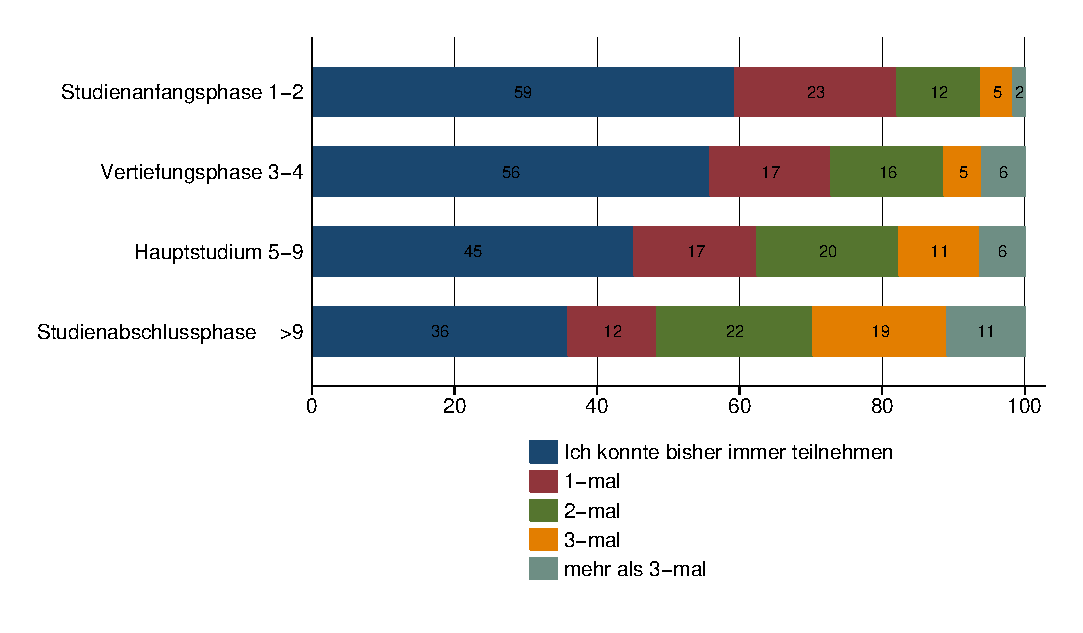
\includegraphics[
%  defaultresolution=72 !,
%  bmpsizefast=false
%]{image}
%\end{verbatim}
% \end{quote}
%
% \subsubsection{Hints}
%
% \begin{itemize}
% \item My version of \xfile{dvips.def} 1999/02/16 v3.0i defines
%       rules for the supported bitmap extensions, but does not
%       include them in the list of extensions that are tried
%       if the file name is not given with an extension.
%       In such a case, the list of extensions can be set
%       by \cs{DeclareGraphicsExtensions}, see \xpackage{grfguide}.
%       The following code just extends the list:
%       \begin{quote}
%\begin{verbatim}
%\makeatletter
%\g@addto@macro\Gin@extensions{,.bmp,.pcx,.msp}
%\makeatother
%\end{verbatim}
%       \end{quote}
% \item My version of \xfile{dvipdfm.def} 1998/11/24 vx.x misses
%       the graphics rule for PNG files. It can be added by:
%       \begin{quote}
%\begin{verbatim}
%\DeclareGraphicsRule{.png}{bmp}{.bb}{#1}
%\end{verbatim}
%       \end{quote}
%       See the previous issue to add the extension \xfile{.png} to the list
%       of extensions for package \xpackage{graphics}.
% \end{itemize}
%
% \subsubsection{Test program}
%
% There is a test program \xfile{bmpsize-test.tex}. Run it through
% \verb|latex|, \verb|pdflatex|, or \verb|pdftex|. Then given
% image files are inspected and the result is printed.
%
% \subsubsection{Interface for programmers}
%
% The macro names of the parsers are \verb|\bmpsize@read@|\meta{type}.
% Example: \cs{bmpsize@read@jpg} in case of JPEG.
%
% A parser sets the switch \cs{ifbmpsize@ok} to true, if it
% could successfully parse the image file.
% The width and height are returnd in \cs{bmpsize@width} and
% \cs{bmpsize@height}. If information about density is available,
% it is used to calculate width and height of the image, otherwise
% the values given by option \xoption{defaultresolution} is used.
% \xoption{resolution} overwrites the values in the image file.
%
% \subsection{Improved bitmap inclusion}
%
% Some drivers for package \xpackage{graphics} define the graphics
% type \xoption{bmp} for bitmap images. The code in the standard
% drivers for \xoption{dvips}, \xoption{dvipdfm}, and \xoption{dvipdfmx}
% is very basic and misses essential features of the
% package \xpackage{graphicx}. Therefore the code for bitmap
% inclusion is automatically rewritten by this package to add
% the following features:
% \begin{itemize}
% \item Support for \xoption{viewport} and \xoption{trim}.
% \item Support for \xoption{clip}.
% \item In case of \xoption{dvipdfm} and \xoption{dvipdfmx} the
%       bitmap images are reused and not included again if they
%       are used more than once.
% \end{itemize}
% However, there is a difference between \xoption{dvipdfm} and
% \xoption{dvipdfmx}, especially if images are reused. In the
% former case the reused box has width and height of 1bp, in the
% latter case its natural width. Thus the correct driver option must be given.
% \xoption{dvipdfm} and \xoption{dvipdfmx} are not equivalent.
%
% Older versions of \xoption{dvipdfmx} uses a size of 1in. However I do
% want to distinguish between versions of the same program. Therefore the
% support of these older versions has stopped with version 1.6 of this package.
% Use version dvipdfmx-20090708 or newer (some few versions before will
% probably also work, but I don't want to investigate this further).
%
% \StopEventually{
% }
%
% \section{Implementation}
%
% \subsection{Basic package \xpackage{bmpsize-base}}
%
%    Identification.
%    \begin{macrocode}
%<*base>
\ProvidesPackage{bmpsize-base}%
  [2009/09/04 v1.6 Basic part of bmpsize (HO)]%
%    \end{macrocode}
%    Modules of package \xpackage{fp} are used for calculations.
%    \begin{macrocode}
\RequirePackage{fp-basic}
\RequirePackage{fp-snap}
%    \end{macrocode}
%    Package \xpackage{fp} uses nested \cs{loop} structures.
%    That breaks with the plain-\TeX\ version of \cs{loop}.
%    Therefore we use the \LaTeX\ variant.
%    \begin{macro}{\@bmpsize@plain@loop}
%    \begin{macrocode}
\long\def\@bmpsize@plain@loop#1\repeat{%
  \def\iterate{%
    #1\relax
    \expandafter\iterate\fi
  }%
  \iterate
  \let\iterate\relax
}
%    \end{macrocode}
%    \end{macro}
%    \begin{macrocode}
\RequirePackage{pdftexcmds}[2007/11/11]
%    \end{macrocode}
%    \begin{macrocode}
\newif\ifbmpsize@ok
\let\@bmpsize@ok\bmpsize@oktrue

\newif\if@bmpsize@bigendian
\newif\if@bmpsize@absnum
\newif\if@bmpsize@user@resolution
\newif\if@bmpsize@fast
\@bmpsize@fasttrue

\def\@bmpsize@init{%
  \let\@bmpsize@org@plain@loop\loop
  \let\loop\@bmpsize@plain@loop
  \bmpsize@okfalse
  \@bmpsize@bigendiantrue
  \@bmpsize@absnumfalse
  \let\bmpsize@pixelwidth\relax
  \let\bmpsize@pixelheight\relax
  \let\bmpsize@pixelx\relax
  \let\bmpsize@pixely\relax
  \let\bmpsize@unit\relax
  \let\bmpsize@pixelxdenom\relax
  \let\bmpsize@pixelydenom\relax
  \let\bmpsize@orientation\relax
}

\def\@bmpsize@stop#1\@nil{}

\def\@bmpsize@loop#1{%
  #1%
  \@bmpsize@loop{#1}%
}
\def\@bmpsize@break#1\@bmpsize@loop#2{}

\def\@bmpsize@size#1#2#3{%
  \edef#3{\pdf@filesize{#1}}%
  \ifx#3\@empty
    \expandafter\@bmpsize@stop
  \fi
  \ifnum#3<#2\relax
    \expandafter\@bmpsize@stop
  \fi
}

\def\@bmpsize@read#1#2#3{%
  \edef\@bmpsize@buf{\pdf@filedump{#3}{#2}{#1}}%
  \edef\@bmpsize@temp{%
    \noexpand\@bmpsize@check@byte{#2}\@bmpsize@buf{}{}\noexpand\\%
  }%
  \@bmpsize@temp
}
\def\@bmpsize@fillbuf#1{%
  \ifx\@bmpsize@buf\@empty
    \expandafter\@firstofone
  \else
    \expandafter\@gobble
  \fi
  {%
    \edef\@bmpsize@buf{%
      \pdf@filedump{\bmpsize@offset}{\bmpsize@fillbuflength}{#1}%
    }%
    \ifx\@bmpsize@buf\@empty
      \expandafter\@bmpsize@stop
    \fi
    \edef\bmpsize@offset{\the\numexpr\bmpsize@offset+\bmpsize@fillbuflength}%
  }%
}
\def\bmpsize@fillbuflength{10}

\def\@bmpsize@append#1#2#3{%
  \edef#1{#2#3}%
}
\def\@bmpsize@pushback#1{%
  \edef\@bmpsize@buf{#1\@bmpsize@buf}%
}

\def\@bmpsize@iswhite#1{%
  \ifnum\pdf@strcmp{#1}{09}=\z@
  \else
    \ifnum\pdf@strcmp{#1}{0A}=\z@
    \else
      \ifnum\pdf@strcmp{#1}{0D}=\z@
      \else
        \ifnum\pdf@strcmp{#1}{20}=\z@
        \else
          1%
        \fi
      \fi
    \fi
  \fi
  \space
}
\def\@bmpsize@isdigit#1{%
  \ifnum\pdf@strcmp{#1}{30}<\z@
    1%
  \else
    \ifnum\pdf@strcmp{#1}{39}>\z@
      1%
    \fi
  \fi
  \space
}

\def\@bmpsize@check@byte#1#2#3{%
  \ifnum#1<\@ne
    \csname fi\endcsname
    \@bmpsize@cleanup@end
  \else
    \csname fi\endcsname
  \ifx!#2#3!%
    \csname fi\endcsname
    \@bmpsize@stop
  \else
    \csname fi\endcsname
    \expandafter\@bmpsize@check@byte\expandafter{\the\numexpr#1-1}%
}
\def\@bmpsize@cleanup@end#1\\{}

\def\@bmpsize@swap@maybe#1{%
  \if@bmpsize@bigendian
  \else
    \edef#1{\expandafter\@bmpsize@@swap#1\@empty\@empty\@empty\@empty}%
  \fi
}
\def\@bmpsize@@swap#1#2#3#4#5#6#7#8{%
  #7#8#5#6#3#4#1#2%
}

\def\@bmpsize@skip@one{%
  \edef\@bmpsize@buf{\expandafter\@gobbletwo\@bmpsize@buf}%
}
\def\@bmpsize@skip@two{%
  \edef\@bmpsize@buf{\expandafter\@gobblefour\@bmpsize@buf}%
}
\def\@bmpsize@skip@four{%
  \edef\@bmpsize@buf{%
    \expandafter\expandafter\expandafter\@gobblefour\expandafter
    \@gobblefour\@bmpsize@buf
  }%
}

\def\@bmpsize@grab#1#2{%
  \edef#1{\noexpand\@bmpsize@grab@byte#2=\@bmpsize@buf\noexpand\\}%
  \edef#1{#1}%
}
\def\@bmpsize@grab@byte#1=#2#3{%
  #2#3%
  \ifnum#1>\@ne
    \expandafter\@bmpsize@grab@byte\the\numexpr#1-1\expandafter=%
  \else
    \expandafter\@bmpsize@cleanup@end
  \fi
}

\def\@bmpsize@abs@maybe#1{%
  \let\@bmpsize@temp\relax
  \if@bmpsize@absnum
    \ifnum"\expandafter\@car#1\@nil>7 %
      \edef#1{\expandafter\@bmpsize@abs@byte#1\relax}%
      \ifnum\pdf@strcmp{#1}{7FFFFFFF}=\z@
        \let\@bmpsize@temp\@bmpsize@stop
      \else
        \def\@bmpsize@temp{\edef#1{\the\numexpr#1+1}}%
      \fi
    \fi
  \fi
}
\def\@bmpsize@abs@byte#1{%
  \ifx#1\relax
  \else
    \ifcase"0#1 %
      F\or E\or D\or C\or B\or A\or 9\or 8\or
      7\or 6\or 5\or 4\or 3\or 2\or 1\or 0%
    \fi
    \expandafter\@bmpsize@abs@byte
  \fi
}

\def\@bmpsize@num@one#1{%
  \@bmpsize@grab#11%
  \@bmpsize@abs@maybe#1%
  \edef#1{\number"#1}%
  \@bmpsize@temp
  \@bmpsize@skip@one
}
\def\@bmpsize@num@two#1{%
  \@bmpsize@grab#12%
  \@bmpsize@swap@maybe#1%
  \@bmpsize@abs@maybe#1%
  \edef#1{\number"#1}%
  \@bmpsize@temp
  \@bmpsize@skip@two
}
\def\@bmpsize@num@four#1{%
  \@bmpsize@grab#14%
  \@bmpsize@swap@maybe#1%
  \@bmpsize@abs@maybe#1%
  \ifnum\pdf@strcmp{#1}{7FFFFFFF}>\z@
    \expandafter\@bmpsize@stop
  \fi
  \edef#1{\number"#1}%
  \@bmpsize@temp
  \@bmpsize@skip@four
}

\def\@bmpsize@div#1#2#3{% #1 := #2/#3
  \FPdiv#1{#2}{#3}%
  \@bmpsize@beautify#1%
}
\def\@bmpsize@beautify#1{%
  \FPifint#1%
    \edef#1{\expandafter\@bmpsize@trunc#1.\@nil}%
  \else
    \edef#1{\expandafter\@bmpsize@cleanup@frac#1.\@nil}%
  \fi
}
\def\@bmpsize@trunc#1.#2\@nil{#1}
% #1 isn't an integer, thus we should have at least one
% necessary digit after the dot
\def\@bmpsize@cleanup@frac#1.#2#3.#4\@nil{%
  #1.#2%
  \ifx\\#3\\%
  \else
    \@bmpsize@cleanup@fracdigits#3000000000\@nil
  \fi
}
\def\@bmpsize@cleanup@fracdigits#1#2#3#4#5#6#7#8#9{%
  \ifcase#9 %
    \ifcase#8 %
      \ifcase#7 %
        \ifcase#6 %
          \ifcase#5 %
            \ifcase #4 %
              \ifcase #3 %
                \ifcase #2 %
                  \ifcase #1 %
                  \else
                    #1%
                  \fi
                \else
                  #1#2%
                \fi
              \else
                #1#2#3%
              \fi
            \else
              #1#2#3#4%
            \fi
          \else
            #1#2#3#4#5%
          \fi
        \else
          #1#2#3#4#5#6%
        \fi
      \else
        #1#2#3#4#5#6#7%
      \fi
    \else
      #1#2#3#4#5#6#7#8%
    \fi
  \else
    #1#2#3#4#5#6#7#8#9%
  \fi
  \@bmpsize@trunc.%
}

\def\@bmpsize@end{%
  \ifbmpsize@ok
    \ifx\bmpsize@pixelwidth\relax
      \bmpsize@okfalse
    \fi
    \ifx\bmpsize@pixelheight\relax
      \bmpsize@okfalse
    \fi
  \fi
  \ifbmpsize@ok
    \ifnum\bmpsize@pixelwidth>\z@
    \else
      \bmpsize@okfalse
    \fi
    \ifnum\bmpsize@pixelheight>\z@
    \else
      \bmpsize@okfalse
    \fi
  \fi
  \ifbmpsize@ok
    \ifcase 0%
      \ifx\bmpsize@pixelx\relax 1 \fi
      \ifx\bmpsize@pixely\relax 1 \fi
      \ifnum\bmpsize@pixelx>\z@\else 1 \fi
      \ifnum\bmpsize@pixely>\z@\else 1 \fi
      \ifx\bmpsize@pixelxdenom\relax
         \ifx\bmpsize@pixelydenom\relax\else 1 \fi
      \else
        \ifnum\bmpsize@pixelxdenom>\z@\else 1 \fi
      \fi
      \ifx\bmpsize@pixelydenom\relax
      \else
        \ifnum\bmpsize@pixelydenom>\z@\else 1 \fi
      \fi
    \else
      \let\bmpsize@pixelx\relax
      \let\bmpsize@pixely\relax
      \let\bmpsize@unit\relax
      \let\bmpsize@pixelxdenom\relax
      \let\bmpsize@pixelydenom\relax
    \fi
    \ifx\bmpsize@pixelxdenom\relax
    \else
      \@bmpsize@div\bmpsize@pixelx\bmpsize@pixelx\bmpsize@pixelxdenom
      \@bmpsize@div\bmpsize@pixely\bmpsize@pixely\bmpsize@pixelydenom
      \let\bmpsize@pixelxdenom\relax
      \let\bmpsize@pixelydenom\relax
    \fi
    \ifcase 0\ifx\bmpsize@unit\relax 1\fi
             \if@bmpsize@user@resolution 1\fi
             \relax
      \let\bmpsize@calc@unit\bmpsize@unit
      \let\bmpsize@calc@pixelx\bmpsize@pixelx
      \let\bmpsize@calc@pixely\bmpsize@pixely
    \else
      \let\bmpsize@calc@unit\bmpsize@unit@default
      \let\bmpsize@calc@pixelx\bmpsize@pixelx@default
      \let\bmpsize@calc@pixely\bmpsize@pixely@default
      \ifx\bmpsize@calc@pixely\Gin@exclamation
        \ifx\bmpsize@pixelx\relax
          \let\bmpsize@calc@pixely\bmpsize@calc@pixelx
        \else
          \FPdiv\bmpsize@calc@pixely\bmpsize@calc@pixelx\bmpsize@pixelx
          \FPmul\bmpsize@calc@pixely\bmpsize@calc@pixely\bmpsize@pixely
        \fi
      \else
        \ifx\bmpsize@calc@pixelx\Gin@exclamation
          \ifx\bmpsize@pixelx\relax
            \let\bmpsize@calc@pixelx\bmpsize@calc@pixely
          \else
            \FPdiv\bmpsize@calc@pixelx\bmpsize@calc@pixely\bmpsize@pixely
            \FPmul\bmpsize@calc@pixelx\bmpsize@calc@pixelx\bmpsize@pixelx
          \fi
        \fi
      \fi
    \fi
    \FPdiv\bmpsize@width\bmpsize@pixelwidth\bmpsize@calc@pixelx
    \FPdiv\bmpsize@height\bmpsize@pixelheight\bmpsize@calc@pixely
    % calculation of width and height in bp for package graphics
    % 1in = 72bp = 72.27pt, 72/72.27 = 8/8.03, 1pt = 65536sp
    \if@bmpsize@fast
      \edef\bmpsize@width{%
        \strip@pt\dimexpr.99626\dimexpr
        \bmpsize@width\dimexpr\bmpsize@calc@unit
      }%
      \edef\bmpsize@height{%
        \strip@pt\dimexpr.99626\dimexpr
        \bmpsize@height\dimexpr\bmpsize@calc@unit
      }%
    \else
      \edef\@bmpsize@temp{\number\dimexpr\bmpsize@calc@unit}%
      \ifnum\@bmpsize@temp>100000 %
        \FPmul\@bmpsize@temp\@bmpsize@temp{0.00001}%
        \def\@bmpsize@corr{100000}%
      \else
        \let\@bmpsize@corr\relax
      \fi
      \FPmul\bmpsize@width\bmpsize@width\@bmpsize@temp
      \FPmul\bmpsize@height\bmpsize@height\@bmpsize@temp
      \FPmul\bmpsize@width\bmpsize@width{8}%
      \FPmul\bmpsize@height\bmpsize@height{8}%
      \FPdiv\bmpsize@width\bmpsize@width{8.03}%
      \FPdiv\bmpsize@height\bmpsize@height{8.03}%
      \FPdiv\bmpsize@width\bmpsize@width{65536}%
      \FPdiv\bmpsize@height\bmpsize@height{65536}%
      \ifx\@bmpsize@corr\relax
      \else
        \FPmul\bmpsize@width\bmpsize@width\@bmpsize@corr
        \FPmul\bmpsize@height\bmpsize@height\@bmpsize@corr
      \fi
      \FPround\bmpsize@width\bmpsize@width{5}%
      \FPround\bmpsize@height\bmpsize@height{5}%
      \@bmpsize@beautify\bmpsize@width
      \@bmpsize@beautify\bmpsize@height
    \fi
  \fi
  \let\loop\@bmpsize@org@plain@loop
}
\def\bmpsize@unit@default{72.27pt}% more accurate than 1in
\def\bmpsize@pixelx@default{72}
\let\bmpsize@pixely@default\Gin@exclamation

\def\bmpsize@types{png,jpg,bmp,gif,tiff,pnm,pam,xpm,tga,pcx,msp,sgi}
%</base>
%    \end{macrocode}
%
% \subsection{Bitmap formats}
%
% \subsubsection{png}
%
%\iffalse
%<*ignore>
%\fi
%\begin{verbatim}
%begin png
%big-endian
%
%read 24 0
%grab 8        -> $temp
%check streq $temp [0x89 "PNG" 0x0D 0x0A 0x1A 0x0A]
%num 4         -> $length
%grab 4        -> $temp
%check streq $temp ["IHDR"]
%num 4         -> $pixelwidth
%num 4         -> $pixelheight
%ok
%assign numexpr(20 + $length) -> $offset
%loop
%  read 8 $offset
%  num 4       -> $length
%  grab 4      -> $temp
%  if streq $temp ["IDAT"]
%    stop
%  fi
%  if streq $temp ["pHYs"]
%    read 9 numexpr($offset + 8)
%    num 4     -> $pixelx
%    num 4     -> $pixely
%    grab 1     -> $temp
%    if numeq $temp 1
%      assign {100cm} -> $unit
%    fi
%    stop
%  fi
%  assign numexpr($offset + 12 + $length) -> $offset
%repeat
%end
%\end{verbatim}
%\iffalse
%</ignore>
%\fi
%    \begin{macro}{\bmpsize@read@png}
%    \begin{macrocode}
%<*base>
\def\bmpsize@read@png#1{%
  \@bmpsize@init
  \@bmpsize@bigendiantrue
  \@bmpsize@read{#1}{24}{0}%
  \@bmpsize@grab\bmpsize@temp{8}%
  \@bmpsize@skip@four
  \@bmpsize@skip@four
  \ifnum\pdf@strcmp{\bmpsize@temp}{89504E470D0A1A0A}=\z@
  \else
    \expandafter\@bmpsize@stop
  \fi
  \@bmpsize@num@four\bmpsize@length
  \@bmpsize@grab\bmpsize@temp{4}%
  \@bmpsize@skip@four
  \ifnum\pdf@strcmp{\bmpsize@temp}{49484452}=\z@
  \else
    \expandafter\@bmpsize@stop
  \fi
  \@bmpsize@num@four\bmpsize@pixelwidth
  \@bmpsize@num@four\bmpsize@pixelheight
  \@bmpsize@ok
  \edef\bmpsize@offset{\the\numexpr20+\bmpsize@length}%
  \@bmpsize@loop{%
    \@bmpsize@read{#1}{8}{\bmpsize@offset}%
    \@bmpsize@num@four\bmpsize@length
    \@bmpsize@grab\bmpsize@temp{4}%
    \@bmpsize@skip@four
    \ifnum\pdf@strcmp{\bmpsize@temp}{49444154}=\z@
      \expandafter\@firstofone
    \else
      \expandafter\@gobble
    \fi
    {%
      \@bmpsize@stop
    }%
    \ifnum\pdf@strcmp{\bmpsize@temp}{70485973}=\z@
      \expandafter\@firstofone
    \else
      \expandafter\@gobble
    \fi
    {%
      \@bmpsize@read{#1}{9}{\numexpr\bmpsize@offset+8\relax}%
      \@bmpsize@num@four\bmpsize@pixelx
      \@bmpsize@num@four\bmpsize@pixely
      \@bmpsize@grab\bmpsize@temp{1}%
      \@bmpsize@skip@one
      \ifnum\bmpsize@temp=1\relax
        \expandafter\@firstofone
      \else
        \expandafter\@gobble
      \fi
      {%
        \def\bmpsize@unit{100cm}%
      }%
      \@bmpsize@stop
    }%
    \edef\bmpsize@offset{\the\numexpr\bmpsize@offset+12+\bmpsize@length}%
  }%
  \@bmpsize@stop
  \@nil
  \@bmpsize@end
}%
%</base>
%    \end{macrocode}
%    \end{macro}
%
% \subsubsection{jpg}
%
%\iffalse
%<*ignore>
%\fi
%\begin{verbatim}
%begin jpg
%
%read 3 0
%grab 3      -> $temp % SOI and 0xFF
%check streq $temp [0xFF 0xD8 0xFF]
%assign {2} -> $offset
%assign {0} -> $exifdensity
%loop
%  read 4 $offset
%  grab 1    -> $temp
%  check streq $temp [0xFF]
%  num 1    -> $temp
%  if numeq $temp 0xDA % SOS
%    stop
%  fi
%  % look for JFIF APP0 segment
%  if numeq $temp 0xE0 % APP0
%    num 2       -> $length
%    if numeq $exifdensity 0
%      if numge $length 16 % a JFIF segment has 16 bytes at least
%        read 12 numexpr($offset + 4)
%        grab 5      -> $temp % identifier
%        if streq $temp ["JFIF" 0x0]
%          check numge $length 16
%          skip 2 % version
%          num 1       -> $temp % units
%          if numeq $temp 1
%            assign {72.27pt} -> $unit
%          else
%            if numeq $temp 2
%              assign {1cm} -> $unit
%            fi
%          fi
%          num 2    -> $pixelx
%          num 2    -> $pixely
%        fi
%      fi
%    fi
%  else
%    if numeq $temp 0xE1 % APP1
%      % look for Exif APP1 segment
%      num 2 -> $length
%      if numge $length 20 % identifier (6) + Tiff header (8) + first IFD (>=6)
%        read 20 numexpr($offset + 4)
%        grab 6 -> $temp
%        if streq $temp ["Exif" 0x0 0x0]
%          assign numexpr($offset + 10) -> $exifoffset
%          % read TIFF header
%          grab 2 -> $temp
%          if streq $temp ["II"]
%            little-endian
%          else
%            check streq $temp ["MM"]
%            % big-endian
%          fi
%          num 2 -> $temp
%          check numeq $temp 42
%          num 4 -> $temp % offset of first IFD
%          check numgt $temp 0
%          % read first IFD
%          assign numexpr($temp + $exifoffset) -> $off
%          read 2 $off
%          num 2 -> $entries
%          assign numexpr($off + 2) -> $off
%          loop
%            if numeq $entries 0
%              break
%            fi
%            assign numexpr($entries - 1) -> $entries
%            % entry format:
%            % 2 tag
%            % 2 field type
%            % 4 count
%            % 4 value/offset
%            read 12 $off
%            assign numexpr($off + 12) -> $off
%            num 2 -> $tag
%            if numeq $tag 296 % ResolutionUnit
%              skip 6 % type: 3 (short), count: 1
%              num 2 -> $temp
%              ifcase $temp
%              or % 1
%                clear $unit
%              or % 2
%                assign {72.27pt} -> $unit
%              or % 3
%                assign {1cm} -> $unit
%              else
%                clear $unit % unknown
%              fi
%              ifcase $temp
%              or % 1
%              or % 2
%                assign {1} -> $exifdensity
%              or % 3
%                assign {1} -> $exifdensity
%              else
%                assign $exifdensity -> $exifdensity
%              fi
%            fi
%            % 256 ImageWidth (use width of JPG part)
%            % 257 ImageHeight (use height of JPG part)
%            if numeq $tag 274 % Orientation
%              skip 6 % type: 3 (short), count: 1
%              num 2 -> $temp
%              if numge $temp 0 
%                if numle $temp 8
%                  assign $temp -> $orientation
%                fi
%              fi
%            fi
%            if numeq $tag 282 % XResolution
%              skip 6
%              num 4 -> $temp
%              read 8 numexpr($temp + $exifoffset)
%              num 4 -> $pixelx
%              num 4 -> $temp
%              if numeq $temp 1
%              else
%                assign numexpr($temp) -> $pixelxdenom
%                % div $pixelx $temp -> $pixelx
%              fi
%            fi
%            if numeq $tag 283 % YResolution
%              skip 6
%              num 4 -> $temp
%              read 8 numexpr($temp + $exifoffset)
%              num 4 -> $pixely
%              num 4 -> $temp
%              if numeq $temp 1
%              else
%                assign numexpr($temp) -> $pixelydenom
%                % div $pixely $temp -> $pixely
%              fi
%            fi
%          repeat
%          big-endian
%        fi
%      fi
%    else
%      assign numexpr($temp - 0xC0) -> $temp
%      ifcase $temp % SOF_0
%      or % SOF_1
%      or % SOF_2
%      or % SOF_3
%      or % DHT
%        assign {-1} -> $temp
%      or % SOF_5
%      or % SOF_6
%      or % SOF_7
%      or % JPG
%        assign {-1} -> $temp
%      or % SOF_9
%      or % SOF_10
%      or % SOF_11
%      or % DAC
%        assign {-1} -> $temp
%      or % SOF_13
%      or % SOF_14
%      or % SOF_15
%      else
%        assign {-1} -> $temp
%      fi
%      if numeq $temp -1
%      else
%        read 4 numexpr($offset + 5)
%        num 2  -> $pixelheight
%        num 2  -> $pixelwidth
%        if numeq $pixelheight 0
%          clear $pixelheight
%          stop
%        fi
%        ok
%        stop
%      fi
%      num 2 -> $length
%    fi
%  fi
%  assign numexpr($offset + $length + 2) -> $offset
%repeat
%end
%\end{verbatim}
%\iffalse
%</ignore>
%\fi
%    \begin{macro}{\bmpsize@read@jpg}
%    \begin{macrocode}
%<*base>
\def\bmpsize@read@jpg#1{%
  \@bmpsize@init
  \@bmpsize@read{#1}{3}{0}%
  \@bmpsize@grab\bmpsize@temp{3}%
  \@bmpsize@skip@two
  \@bmpsize@skip@one
  \ifnum\pdf@strcmp{\bmpsize@temp}{FFD8FF}=\z@
  \else
    \expandafter\@bmpsize@stop
  \fi
  \def\bmpsize@offset{2}%
  \def\bmpsize@exifdensity{0}%
  \@bmpsize@loop{%
    \@bmpsize@read{#1}{4}{\bmpsize@offset}%
    \@bmpsize@grab\bmpsize@temp{1}%
    \@bmpsize@skip@one
    \ifnum\pdf@strcmp{\bmpsize@temp}{FF}=\z@
    \else
      \expandafter\@bmpsize@stop
    \fi
    \@bmpsize@num@one\bmpsize@temp
    \ifnum\bmpsize@temp=218\relax
      \expandafter\@firstofone
    \else
      \expandafter\@gobble
    \fi
    {%
      \@bmpsize@stop
    }%
    \ifnum\bmpsize@temp=224\relax
      \expandafter\@firstoftwo
    \else
      \expandafter\@secondoftwo
    \fi
    {%
      \@bmpsize@num@two\bmpsize@length
      \ifnum\bmpsize@exifdensity=0\relax
        \expandafter\@firstofone
      \else
        \expandafter\@gobble
      \fi
      {%
        \unless\ifnum\bmpsize@length<16\relax
          \expandafter\@firstofone
        \else
          \expandafter\@gobble
        \fi
        {%
          \@bmpsize@read{#1}{12}{\numexpr\bmpsize@offset+4\relax}%
          \@bmpsize@grab\bmpsize@temp{5}%
          \@bmpsize@skip@four
          \@bmpsize@skip@one
          \ifnum\pdf@strcmp{\bmpsize@temp}{4A46494600}=\z@
            \expandafter\@firstofone
          \else
            \expandafter\@gobble
          \fi
          {%
            \ifnum\bmpsize@length<16\relax
              \expandafter\@bmpsize@stop
            \fi
            \@bmpsize@skip@two
            \@bmpsize@num@one\bmpsize@temp
            \ifnum\bmpsize@temp=1\relax
              \expandafter\@firstoftwo
            \else
              \expandafter\@secondoftwo
            \fi
            {%
              \def\bmpsize@unit{72.27pt}%
            }{%
              \ifnum\bmpsize@temp=2\relax
                \expandafter\@firstofone
              \else
                \expandafter\@gobble
              \fi
              {%
                \def\bmpsize@unit{1cm}%
              }%
            }%
            \@bmpsize@num@two\bmpsize@pixelx
            \@bmpsize@num@two\bmpsize@pixely
          }%
        }%
      }%
    }{%
      \ifnum\bmpsize@temp=225\relax
        \expandafter\@firstoftwo
      \else
        \expandafter\@secondoftwo
      \fi
      {%
        \@bmpsize@num@two\bmpsize@length
        \unless\ifnum\bmpsize@length<20\relax
          \expandafter\@firstofone
        \else
          \expandafter\@gobble
        \fi
        {%
          \@bmpsize@read{#1}{20}{\numexpr\bmpsize@offset+4\relax}%
          \@bmpsize@grab\bmpsize@temp{6}%
          \@bmpsize@skip@four
          \@bmpsize@skip@two
          \ifnum\pdf@strcmp{\bmpsize@temp}{457869660000}=\z@
            \expandafter\@firstofone
          \else
            \expandafter\@gobble
          \fi
          {%
            \edef\bmpsize@exifoffset{\the\numexpr\bmpsize@offset+10}%
            \@bmpsize@grab\bmpsize@temp{2}%
            \@bmpsize@skip@two
            \ifnum\pdf@strcmp{\bmpsize@temp}{4949}=\z@
              \expandafter\@firstoftwo
            \else
              \expandafter\@secondoftwo
            \fi
            {%
              \@bmpsize@bigendianfalse
            }{%
              \ifnum\pdf@strcmp{\bmpsize@temp}{4D4D}=\z@
              \else
                \expandafter\@bmpsize@stop
              \fi
            }%
            \@bmpsize@num@two\bmpsize@temp
            \ifnum\bmpsize@temp=42\relax
            \else
              \expandafter\@bmpsize@stop
            \fi
            \@bmpsize@num@four\bmpsize@temp
            \ifnum\bmpsize@temp>0\relax
            \else
              \expandafter\@bmpsize@stop
            \fi
            \edef\bmpsize@off{\the\numexpr\bmpsize@temp+\bmpsize@exifoffset}%
            \@bmpsize@read{#1}{2}{\bmpsize@off}%
            \@bmpsize@num@two\bmpsize@entries
            \edef\bmpsize@off{\the\numexpr\bmpsize@off+2}%
            \@bmpsize@loop{%
              \ifnum\bmpsize@entries=0\relax
                \expandafter\@firstofone
              \else
                \expandafter\@gobble
              \fi
              {%
                \@bmpsize@break
              }%
              \edef\bmpsize@entries{\the\numexpr\bmpsize@entries-1}%
              \@bmpsize@read{#1}{12}{\bmpsize@off}%
              \edef\bmpsize@off{\the\numexpr\bmpsize@off+12}%
              \@bmpsize@num@two\bmpsize@tag
              \ifnum\bmpsize@tag=296\relax
                \expandafter\@firstofone
              \else
                \expandafter\@gobble
              \fi
              {%
                \@bmpsize@skip@four
                \@bmpsize@skip@two
                \@bmpsize@num@two\bmpsize@temp
                \ifcase\bmpsize@temp\relax
                \or
                  \let\bmpsize@unit\relax
                \or
                  \def\bmpsize@unit{72.27pt}%
                \or
                  \def\bmpsize@unit{1cm}%
                \else
                  \let\bmpsize@unit\relax
                \fi
                \ifcase\bmpsize@temp\relax
                \or
                \or
                  \def\bmpsize@exifdensity{1}%
                \or
                  \def\bmpsize@exifdensity{1}%
                \else
                  \let\bmpsize@exifdensity\bmpsize@exifdensity
                \fi
              }%
              \ifnum\bmpsize@tag=274\relax
                \expandafter\@firstofone
              \else
                \expandafter\@gobble
              \fi
              {%
                \@bmpsize@skip@four
                \@bmpsize@skip@two
                \@bmpsize@num@two\bmpsize@temp
                \unless\ifnum\bmpsize@temp<0\relax
                  \expandafter\@firstofone
                \else
                  \expandafter\@gobble
                \fi
                {%
                  \unless\ifnum\bmpsize@temp>8\relax
                    \expandafter\@firstofone
                  \else
                    \expandafter\@gobble
                  \fi
                  {%
                    \let\bmpsize@orientation\bmpsize@temp
                  }%
                }%
              }%
              \ifnum\bmpsize@tag=282\relax
                \expandafter\@firstofone
              \else
                \expandafter\@gobble
              \fi
              {%
                \@bmpsize@skip@four
                \@bmpsize@skip@two
                \@bmpsize@num@four\bmpsize@temp
                \@bmpsize@read{#1}{8}{\numexpr\bmpsize@temp+\bmpsize@exifoffset\relax}%
                \@bmpsize@num@four\bmpsize@pixelx
                \@bmpsize@num@four\bmpsize@temp
                \ifnum\bmpsize@temp=1\relax
                  \expandafter\@gobble
                \else
                  \expandafter\@firstofone
                \fi
                {%
                  \edef\bmpsize@pixelxdenom{\the\numexpr\bmpsize@temp}%
                }%
              }%
              \ifnum\bmpsize@tag=283\relax
                \expandafter\@firstofone
              \else
                \expandafter\@gobble
              \fi
              {%
                \@bmpsize@skip@four
                \@bmpsize@skip@two
                \@bmpsize@num@four\bmpsize@temp
                \@bmpsize@read{#1}{8}{\numexpr\bmpsize@temp+\bmpsize@exifoffset\relax}%
                \@bmpsize@num@four\bmpsize@pixely
                \@bmpsize@num@four\bmpsize@temp
                \ifnum\bmpsize@temp=1\relax
                  \expandafter\@gobble
                \else
                  \expandafter\@firstofone
                \fi
                {%
                  \edef\bmpsize@pixelydenom{\the\numexpr\bmpsize@temp}%
                }%
              }%
            }%
            \@bmpsize@bigendiantrue
          }%
        }%
      }{%
        \edef\bmpsize@temp{\the\numexpr\bmpsize@temp-192}%
        \ifcase\bmpsize@temp\relax
        \or
        \or
        \or
        \or
          \def\bmpsize@temp{-1}%
        \or
        \or
        \or
        \or
          \def\bmpsize@temp{-1}%
        \or
        \or
        \or
        \or
          \def\bmpsize@temp{-1}%
        \or
        \or
        \or
        \else
          \def\bmpsize@temp{-1}%
        \fi
        \ifnum\bmpsize@temp=-1\relax
          \expandafter\@gobble
        \else
          \expandafter\@firstofone
        \fi
        {%
          \@bmpsize@read{#1}{4}{\numexpr\bmpsize@offset+5\relax}%
          \@bmpsize@num@two\bmpsize@pixelheight
          \@bmpsize@num@two\bmpsize@pixelwidth
          \ifnum\bmpsize@pixelheight=0\relax
            \expandafter\@firstofone
          \else
            \expandafter\@gobble
          \fi
          {%
            \let\bmpsize@pixelheight\relax
            \@bmpsize@stop
          }%
          \@bmpsize@ok
          \@bmpsize@stop
        }%
        \@bmpsize@num@two\bmpsize@length
      }%
    }%
    \edef\bmpsize@offset{\the\numexpr\bmpsize@offset+\bmpsize@length+2}%
  }%
  \@bmpsize@stop
  \@nil
  \@bmpsize@end
}%
%</base>
%    \end{macrocode}
%    \end{macro}
%
% \subsubsection{bmp}
%
%\iffalse
%<*ignore>
%\fi
%\begin{verbatim}
%begin bmp
%little-endian
%
%read 26 0
%grab 2 -> $temp
%check streq $temp ["BM"]
%skip 12
%% header size is 4 bytes in V3+, unknown for V1, V2,
%% known header sizes fit in 2 bytes
%num 2   -> $temp
%if numeq $temp 12 % V1
%  skip 2
%  num 2 -> $pixelwidth
%  num 2 -> $pixelheight
%  % no resolution entries
%  ok
%  stop
%fi
%if numeq $temp 64 % V2
%  skip 2
%  num 2 -> $pixelwidth
%  num 2 -> $pixelheight
%  % missing specification for resolution
%  ok
%  stop
%fi
%% V3, V4, V5
%skip 2
%num 4 -> $pixelwidth
%absnum 4 -> $pixelheight
%ok
%read 8 38
%num 4 -> $pixelx
%num 4 -> $pixely
%assign {100cm} -> $unit
%end
%\end{verbatim}
%\iffalse
%</ignore>
%\fi
%    \begin{macro}{\bmpsize@read@bmp}
%    \begin{macrocode}
%<*base>
\def\bmpsize@read@bmp#1{%
  \@bmpsize@init
  \@bmpsize@bigendianfalse
  \@bmpsize@read{#1}{26}{0}%
  \@bmpsize@grab\bmpsize@temp{2}%
  \@bmpsize@skip@two
  \ifnum\pdf@strcmp{\bmpsize@temp}{424D}=\z@
  \else
    \expandafter\@bmpsize@stop
  \fi
  \@bmpsize@skip@four
  \@bmpsize@skip@four
  \@bmpsize@skip@four
  \@bmpsize@num@two\bmpsize@temp
  \ifnum\bmpsize@temp=12\relax
    \expandafter\@firstofone
  \else
    \expandafter\@gobble
  \fi
  {%
    \@bmpsize@skip@two
    \@bmpsize@num@two\bmpsize@pixelwidth
    \@bmpsize@num@two\bmpsize@pixelheight
    \@bmpsize@ok
    \@bmpsize@stop
  }%
  \ifnum\bmpsize@temp=64\relax
    \expandafter\@firstofone
  \else
    \expandafter\@gobble
  \fi
  {%
    \@bmpsize@skip@two
    \@bmpsize@num@two\bmpsize@pixelwidth
    \@bmpsize@num@two\bmpsize@pixelheight
    \@bmpsize@ok
    \@bmpsize@stop
  }%
  \@bmpsize@skip@two
  \@bmpsize@num@four\bmpsize@pixelwidth
  \@bmpsize@absnumtrue
  \@bmpsize@num@four\bmpsize@pixelheight
  \@bmpsize@absnumfalse
  \@bmpsize@ok
  \@bmpsize@read{#1}{8}{38}%
  \@bmpsize@num@four\bmpsize@pixelx
  \@bmpsize@num@four\bmpsize@pixely
  \def\bmpsize@unit{100cm}%
  \@bmpsize@stop
  \@nil
  \@bmpsize@end
}%
%</base>
%    \end{macrocode}
%    \end{macro}
%
% \subsubsection{gif}
%
%\iffalse
%<*ignore>
%\fi
%\begin{verbatim}
%begin gif
%little-endian
%
%% Header
%read 13 0
%grab 3      -> $temp
%check streq $temp ["GIF"]
%skip 3      % version
%
%% Logical Screen Descriptor
%num 2       -> $pixelwidth
%num 2       -> $pixelheight
%skip 2
%num 1       -> $temp % Pixel Aspect Ratio
%if numeq $temp 0
%else
%  assign numexpr($temp + 15) -> $pixelx
%  assign {64}     -> $pixely
%fi
%ok
%end
%\end{verbatim}
%\iffalse
%</ignore>
%\fi
%    \begin{macro}{\bmpsize@read@gif}
%    \begin{macrocode}
%<*base>
\def\bmpsize@read@gif#1{%
  \@bmpsize@init
  \@bmpsize@bigendianfalse
  \@bmpsize@read{#1}{13}{0}%
  \@bmpsize@grab\bmpsize@temp{3}%
  \@bmpsize@skip@two
  \@bmpsize@skip@one
  \ifnum\pdf@strcmp{\bmpsize@temp}{474946}=\z@
  \else
    \expandafter\@bmpsize@stop
  \fi
  \@bmpsize@skip@two
  \@bmpsize@skip@one
  \@bmpsize@num@two\bmpsize@pixelwidth
  \@bmpsize@num@two\bmpsize@pixelheight
  \@bmpsize@skip@two
  \@bmpsize@num@one\bmpsize@temp
  \ifnum\bmpsize@temp=0\relax
    \expandafter\@gobble
  \else
    \expandafter\@firstofone
  \fi
  {%
    \edef\bmpsize@pixelx{\the\numexpr\bmpsize@temp+15}%
    \def\bmpsize@pixely{64}%
  }%
  \@bmpsize@ok
  \@bmpsize@stop
  \@nil
  \@bmpsize@end
}%
%</base>
%    \end{macrocode}
%    \end{macro}
%
% \subsubsection{tiff}
%
%\iffalse
%<*ignore>
%\fi
%\begin{verbatim}
%begin tiff
%% defaults
%assign {72.27pt} -> $unit
%
%% Image File Header
%read 8 0
%grab 2 -> $temp
%if streq $temp ["II"]
%  little-endian
%else
%  check streq $temp ["MM"]
%  big-endian
%fi
%num 2 -> $temp
%check numeq $temp 42
%num 4 -> $offset % first IFD (Image File Directory)
%
%% First IFD
%read 2 $offset
%assign numexpr($offset + 2) -> $offset
%num 2 -> $entries
%ok % must rely on checks at the end
%loop
%  if numeq $entries 0
%    stop
%  fi
%  assign numexpr($entries - 1) -> $entries
%  % entry format:
%  % 2 tag
%  % 2 field type
%  % 4 count
%  % 4 value/offset
%  read 12 $offset
%  assign numexpr($offset + 12) -> $offset
%  num 2 -> $tag % tag
%  if numeq $temp 296 % ResolutionUnit
%    skip 6 % type: 3 (short), count: 1
%    num 2 -> $temp
%    ifcase $temp
%    or % 1
%      clear $unit
%    or % 2
%      assign {72.27pt} -> $unit
%    or % 3
%      assign {1cm} -> $unit
%    else
%      clear $unit
%    fi
%  fi
%  if numeq $tag 256 % ImageWidth
%    skip 6
%    num 4 -> $pixelwidth
%  fi
%  if numeq $tag 257 % ImageLength
%    skip 6
%    num 4 -> $pixelheight
%  fi
%  if numeq $tag 282 % XResolution
%    skip 6
%    num 4 -> $temp
%    read 8 $temp
%    num 4 -> $pixelx
%    num 4 -> $temp
%    if numeq $temp 1
%    else
%      assign numexpr($temp) -> $pixelxdenom
%      % div $pixelx $temp -> $pixelx
%    fi
%  fi
%  if numeq $tag 283 % YResolution
%    skip 6
%    num 4 -> $temp
%    read 8 $temp
%    num 4 -> $pixely
%    num 4 -> $temp
%    if numeq $temp 1
%    else
%      assign numexpr($temp) -> $pixelydenom
%      % div $pixely $temp -> $pixely
%    fi
%  fi
%repeat
%end
%\end{verbatim}
%\iffalse
%</ignore>
%\fi
%    \begin{macro}{\bmpsize@read@tiff}
%    \begin{macrocode}
%<*base>
\def\bmpsize@read@tiff#1{%
  \@bmpsize@init
  \def\bmpsize@unit{72.27pt}%
  \@bmpsize@read{#1}{8}{0}%
  \@bmpsize@grab\bmpsize@temp{2}%
  \@bmpsize@skip@two
  \ifnum\pdf@strcmp{\bmpsize@temp}{4949}=\z@
    \expandafter\@firstoftwo
  \else
    \expandafter\@secondoftwo
  \fi
  {%
    \@bmpsize@bigendianfalse
  }{%
    \ifnum\pdf@strcmp{\bmpsize@temp}{4D4D}=\z@
    \else
      \expandafter\@bmpsize@stop
    \fi
    \@bmpsize@bigendiantrue
  }%
  \@bmpsize@num@two\bmpsize@temp
  \ifnum\bmpsize@temp=42\relax
  \else
    \expandafter\@bmpsize@stop
  \fi
  \@bmpsize@num@four\bmpsize@offset
  \@bmpsize@read{#1}{2}{\bmpsize@offset}%
  \edef\bmpsize@offset{\the\numexpr\bmpsize@offset+2}%
  \@bmpsize@num@two\bmpsize@entries
  \@bmpsize@ok
  \@bmpsize@loop{%
    \ifnum\bmpsize@entries=0\relax
      \expandafter\@firstofone
    \else
      \expandafter\@gobble
    \fi
    {%
      \@bmpsize@stop
    }%
    \edef\bmpsize@entries{\the\numexpr\bmpsize@entries-1}%
    \@bmpsize@read{#1}{12}{\bmpsize@offset}%
    \edef\bmpsize@offset{\the\numexpr\bmpsize@offset+12}%
    \@bmpsize@num@two\bmpsize@tag
    \ifnum\bmpsize@temp=296\relax
      \expandafter\@firstofone
    \else
      \expandafter\@gobble
    \fi
    {%
      \@bmpsize@skip@four
      \@bmpsize@skip@two
      \@bmpsize@num@two\bmpsize@temp
      \ifcase\bmpsize@temp\relax
      \or
        \let\bmpsize@unit\relax
      \or
        \def\bmpsize@unit{72.27pt}%
      \or
        \def\bmpsize@unit{1cm}%
      \else
        \let\bmpsize@unit\relax
      \fi
    }%
    \ifnum\bmpsize@tag=256\relax
      \expandafter\@firstofone
    \else
      \expandafter\@gobble
    \fi
    {%
      \@bmpsize@skip@four
      \@bmpsize@skip@two
      \@bmpsize@num@four\bmpsize@pixelwidth
    }%
    \ifnum\bmpsize@tag=257\relax
      \expandafter\@firstofone
    \else
      \expandafter\@gobble
    \fi
    {%
      \@bmpsize@skip@four
      \@bmpsize@skip@two
      \@bmpsize@num@four\bmpsize@pixelheight
    }%
    \ifnum\bmpsize@tag=282\relax
      \expandafter\@firstofone
    \else
      \expandafter\@gobble
    \fi
    {%
      \@bmpsize@skip@four
      \@bmpsize@skip@two
      \@bmpsize@num@four\bmpsize@temp
      \@bmpsize@read{#1}{8}{\bmpsize@temp}%
      \@bmpsize@num@four\bmpsize@pixelx
      \@bmpsize@num@four\bmpsize@temp
      \ifnum\bmpsize@temp=1\relax
        \expandafter\@gobble
      \else
        \expandafter\@firstofone
      \fi
      {%
        \edef\bmpsize@pixelxdenom{\the\numexpr\bmpsize@temp}%
      }%
    }%
    \ifnum\bmpsize@tag=283\relax
      \expandafter\@firstofone
    \else
      \expandafter\@gobble
    \fi
    {%
      \@bmpsize@skip@four
      \@bmpsize@skip@two
      \@bmpsize@num@four\bmpsize@temp
      \@bmpsize@read{#1}{8}{\bmpsize@temp}%
      \@bmpsize@num@four\bmpsize@pixely
      \@bmpsize@num@four\bmpsize@temp
      \ifnum\bmpsize@temp=1\relax
        \expandafter\@gobble
      \else
        \expandafter\@firstofone
      \fi
      {%
        \edef\bmpsize@pixelydenom{\the\numexpr\bmpsize@temp}%
      }%
    }%
  }%
  \@bmpsize@stop
  \@nil
  \@bmpsize@end
}%
%</base>
%    \end{macrocode}
%    \end{macro}
%
% \subsubsection{pnm}
%
%\iffalse
%<*ignore>
%\fi
%\begin{verbatim}
%begin pnm
%assign {0} -> $offset
%read 3 $offset
%assign {3} -> $offset
%grab 1 -> $temp
%check streq $temp ["P"]
%grab 1 -> $temp
%check strge $temp ["1"]
%check strle $temp ["6"]
%% ensure one white space
%grab 1 -> $temp
%if iswhite $temp
%else
%  stop
%fi
%loop
%  % skip white space
%  fillbuf
%  grab 1 -> $temp
%  if iswhite $temp
%  else
%    if streq $temp ["#"]
%      % ignore comments
%      loop
%        fillbuf
%        grab 1 -> $temp
%        if streq $temp [0x0A]
%          break
%        else
%          if streq $temp [0x0D]
%            break
%          fi
%        fi
%      repeat
%    else
%      pushback $temp
%      break
%    fi
%  fi
%repeat
%assign {} -> $tempnum
%loop
%  fillbuf
%  grab 1 -> $temp
%  if isdigit $temp
%    append $tempnum $temp -> $tempnum
%  else
%    if iswhite $temp
%      break
%    else
%      stop
%    fi
%  fi
%repeat
%assign unescapehex($tempnum) -> $pixelwidth
%loop
%  fillbuf
%  grab 1 -> $temp
%  if iswhite $temp
%  else
%    pushback $temp
%    break
%  fi
%repeat
%assign {} -> $tempnum
%loop
%  fillbuf
%  grab 1 -> $temp
%  if isdigit $temp
%    append $tempnum $temp -> $tempnum
%  else
%    if iswhite $temp
%      break
%    else
%      stop
%    fi
%  fi
%repeat
%assign unescapehex($tempnum) -> $pixelheight
%ok
%end
%\end{verbatim}
%\iffalse
%</ignore>
%\fi
%    \begin{macro}{\bmpsize@read@pnm}
%    \begin{macrocode}
%<*base>
\def\bmpsize@read@pnm#1{%
  \@bmpsize@init
  \def\bmpsize@offset{0}%
  \@bmpsize@read{#1}{3}{\bmpsize@offset}%
  \def\bmpsize@offset{3}%
  \@bmpsize@grab\bmpsize@temp{1}%
  \@bmpsize@skip@one
  \ifnum\pdf@strcmp{\bmpsize@temp}{50}=\z@
  \else
    \expandafter\@bmpsize@stop
  \fi
  \@bmpsize@grab\bmpsize@temp{1}%
  \@bmpsize@skip@one
  \ifnum\pdf@strcmp{\bmpsize@temp}{31}<\z@
    \expandafter\@bmpsize@stop
  \fi
  \ifnum\pdf@strcmp{\bmpsize@temp}{36}>\z@
    \expandafter\@bmpsize@stop
  \fi
  \@bmpsize@grab\bmpsize@temp{1}%
  \@bmpsize@skip@one
  \ifcase 0\@bmpsize@iswhite\bmpsize@temp
    \expandafter\@gobble
  \else
    \expandafter\@firstofone
  \fi
  {%
    \@bmpsize@stop
  }%
  \@bmpsize@loop{%
    \@bmpsize@fillbuf{#1}%
    \@bmpsize@grab\bmpsize@temp{1}%
    \@bmpsize@skip@one
    \ifcase 0\@bmpsize@iswhite\bmpsize@temp
      \expandafter\@gobble
    \else
      \expandafter\@firstofone
    \fi
    {%
      \ifnum\pdf@strcmp{\bmpsize@temp}{23}=\z@
        \expandafter\@firstoftwo
      \else
        \expandafter\@secondoftwo
      \fi
      {%
        \@bmpsize@loop{%
          \@bmpsize@fillbuf{#1}%
          \@bmpsize@grab\bmpsize@temp{1}%
          \@bmpsize@skip@one
          \ifnum\pdf@strcmp{\bmpsize@temp}{0A}=\z@
            \expandafter\@firstoftwo
          \else
            \expandafter\@secondoftwo
          \fi
          {%
            \@bmpsize@break
          }{%
            \ifnum\pdf@strcmp{\bmpsize@temp}{0D}=\z@
              \expandafter\@firstofone
            \else
              \expandafter\@gobble
            \fi
            {%
              \@bmpsize@break
            }%
          }%
        }%
      }{%
        \@bmpsize@pushback\bmpsize@temp
        \@bmpsize@break
      }%
    }%
  }%
  \def\bmpsize@tempnum{}%
  \@bmpsize@loop{%
    \@bmpsize@fillbuf{#1}%
    \@bmpsize@grab\bmpsize@temp{1}%
    \@bmpsize@skip@one
    \ifcase 0\@bmpsize@isdigit\bmpsize@temp
      \expandafter\@firstoftwo
    \else
      \expandafter\@secondoftwo
    \fi
    {%
      \@bmpsize@append\bmpsize@tempnum\bmpsize@tempnum\bmpsize@temp
    }{%
      \ifcase 0\@bmpsize@iswhite\bmpsize@temp
        \expandafter\@firstoftwo
      \else
        \expandafter\@secondoftwo
      \fi
      {%
        \@bmpsize@break
      }{%
        \@bmpsize@stop
      }%
    }%
  }%
  \edef\bmpsize@pixelwidth{\pdf@unescapehex{\bmpsize@tempnum}}%
  \@bmpsize@loop{%
    \@bmpsize@fillbuf{#1}%
    \@bmpsize@grab\bmpsize@temp{1}%
    \@bmpsize@skip@one
    \ifcase 0\@bmpsize@iswhite\bmpsize@temp
      \expandafter\@gobble
    \else
      \expandafter\@firstofone
    \fi
    {%
      \@bmpsize@pushback\bmpsize@temp
      \@bmpsize@break
    }%
  }%
  \def\bmpsize@tempnum{}%
  \@bmpsize@loop{%
    \@bmpsize@fillbuf{#1}%
    \@bmpsize@grab\bmpsize@temp{1}%
    \@bmpsize@skip@one
    \ifcase 0\@bmpsize@isdigit\bmpsize@temp
      \expandafter\@firstoftwo
    \else
      \expandafter\@secondoftwo
    \fi
    {%
      \@bmpsize@append\bmpsize@tempnum\bmpsize@tempnum\bmpsize@temp
    }{%
      \ifcase 0\@bmpsize@iswhite\bmpsize@temp
        \expandafter\@firstoftwo
      \else
        \expandafter\@secondoftwo
      \fi
      {%
        \@bmpsize@break
      }{%
        \@bmpsize@stop
      }%
    }%
  }%
  \edef\bmpsize@pixelheight{\pdf@unescapehex{\bmpsize@tempnum}}%
  \@bmpsize@ok
  \@bmpsize@stop
  \@nil
  \@bmpsize@end
}%
%</base>
%    \end{macrocode}
%    \end{macro}
%
% \subsubsection{pam}
%
%\iffalse
%<*ignore>
%\fi
%\begin{verbatim}
%begin pam
%read 3 0
%assign {3} -> $offset
%assign $offset -> $off
%grab 3 -> $temp
%check streq $temp ["P7" 0x0A]
%loop
%  fillbuf
%  grab 1 -> $temp
%  if iswhite $temp
%    % ignore white space
%    assign numexpr($off + 1) -> $off
%  else
%    if streq $temp ["#"]
%      % ignore comment line
%      assign numexpr($off + 1) -> $off
%      loop
%        fillbuf
%        grab 1 -> $temp
%        assign numexpr($off + 1) -> $off
%        if streq $temp [0x0A]
%          break
%        fi
%      repeat
%    else
%      read 6 $off
%      assign numexpr($off + 6) -> $offset
%      grab 5 -> $head
%      if streq $head ["WIDTH"]
%        assign numexpr($off + 5) -> $off
%        % skip white space
%        loop
%          fillbuf
%          grab 1 -> $temp
%          if iswhite $temp
%            assign numexpr($off + 1) -> $off
%          else
%            if isdigit $temp
%              assign numexpr($off + 1) -> $off
%              break
%            else
%              % error
%              stop
%            fi
%          fi
%        repeat
%        % read number
%        assign $temp -> $tempnum
%        loop
%          fillbuf
%          grab 1 -> $temp
%          if isdigit $temp
%            assign numexpr($off + 1) -> $off
%            append $tempnum $temp -> $tempnum
%          else
%            pushback $temp
%            break
%          fi
%        repeat
%        % skip to end of line
%        loop
%          fillbuf
%          grab 1 -> $temp
%          assign numexpr($off + 1) -> $off
%          if streq $temp [0x0A]
%            break
%          fi
%        repeat
%        assign unescapehex($tempnum) -> $pixelwidth
%      else
%        grab 1 -> $temp
%        append $head $temp -> $head
%        if streq $head ["ENDHDR"]
%          % last header line
%          ok
%          stop
%        else
%          if streq $head ["HEIGHT"]
%            assign numexpr($off + 6) -> $off
%            % skip white space
%            loop
%              fillbuf
%              grab 1 -> $temp
%              if iswhite $temp
%                assign numexpr($off + 1) -> $off
%              else
%                if isdigit $temp
%                  assign numexpr($off + 1) -> $off
%                  break
%                else
%                  % error
%                  stop
%                fi
%              fi
%            repeat
%            % read number
%            assign $temp -> $tempnum
%            loop
%              fillbuf
%              grab 1 -> $temp
%              if isdigit $temp
%                assign numexpr($off + 1) -> $off
%                append $tempnum $temp -> $tempnum
%              else
%                pushback $temp
%                break
%              fi
%            repeat
%            % skip to end of line
%            loop
%              fillbuf
%              grab 1 -> $temp
%              assign numexpr($off + 1) -> $off
%              if streq $temp [0x0A]
%                break
%              fi
%            repeat
%            assign unescapehex($tempnum) -> $pixelheight
%          else
%            % ignore unknown header line
%            pushback $head
%            loop
%              fillbuf
%              grab 1 -> $temp
%              assign numexpr($off + 1) -> $off
%              if streq $temp [0x0A]
%                break
%              fi
%            repeat
%          fi
%        fi
%      fi
%    fi
%  fi
%repeat
%end
%\end{verbatim}
%\iffalse
%</ignore>
%\fi
%    \begin{macro}{\bmpsize@read@pam}
%    \begin{macrocode}
%<*base>
\def\bmpsize@read@pam#1{%
  \@bmpsize@init
  \@bmpsize@read{#1}{3}{0}%
  \def\bmpsize@offset{3}%
  \let\bmpsize@off\bmpsize@offset
  \@bmpsize@grab\bmpsize@temp{3}%
  \@bmpsize@skip@two
  \@bmpsize@skip@one
  \ifnum\pdf@strcmp{\bmpsize@temp}{50370A}=\z@
  \else
    \expandafter\@bmpsize@stop
  \fi
  \@bmpsize@loop{%
    \@bmpsize@fillbuf{#1}%
    \@bmpsize@grab\bmpsize@temp{1}%
    \@bmpsize@skip@one
    \ifcase 0\@bmpsize@iswhite\bmpsize@temp
      \expandafter\@firstoftwo
    \else
      \expandafter\@secondoftwo
    \fi
    {%
      \edef\bmpsize@off{\the\numexpr\bmpsize@off+1}%
    }{%
      \ifnum\pdf@strcmp{\bmpsize@temp}{23}=\z@
        \expandafter\@firstoftwo
      \else
        \expandafter\@secondoftwo
      \fi
      {%
        \edef\bmpsize@off{\the\numexpr\bmpsize@off+1}%
        \@bmpsize@loop{%
          \@bmpsize@fillbuf{#1}%
          \@bmpsize@grab\bmpsize@temp{1}%
          \@bmpsize@skip@one
          \edef\bmpsize@off{\the\numexpr\bmpsize@off+1}%
          \ifnum\pdf@strcmp{\bmpsize@temp}{0A}=\z@
            \expandafter\@firstofone
          \else
            \expandafter\@gobble
          \fi
          {%
            \@bmpsize@break
          }%
        }%
      }{%
        \@bmpsize@read{#1}{6}{\bmpsize@off}%
        \edef\bmpsize@offset{\the\numexpr\bmpsize@off+6}%
        \@bmpsize@grab\bmpsize@head{5}%
        \@bmpsize@skip@four
        \@bmpsize@skip@one
        \ifnum\pdf@strcmp{\bmpsize@head}{5749445448}=\z@
          \expandafter\@firstoftwo
        \else
          \expandafter\@secondoftwo
        \fi
        {%
          \edef\bmpsize@off{\the\numexpr\bmpsize@off+5}%
          \@bmpsize@loop{%
            \@bmpsize@fillbuf{#1}%
            \@bmpsize@grab\bmpsize@temp{1}%
            \@bmpsize@skip@one
            \ifcase 0\@bmpsize@iswhite\bmpsize@temp
              \expandafter\@firstoftwo
            \else
              \expandafter\@secondoftwo
            \fi
            {%
              \edef\bmpsize@off{\the\numexpr\bmpsize@off+1}%
            }{%
              \ifcase 0\@bmpsize@isdigit\bmpsize@temp
                \expandafter\@firstoftwo
              \else
                \expandafter\@secondoftwo
              \fi
              {%
                \edef\bmpsize@off{\the\numexpr\bmpsize@off+1}%
                \@bmpsize@break
              }{%
                \@bmpsize@stop
              }%
            }%
          }%
          \let\bmpsize@tempnum\bmpsize@temp
          \@bmpsize@loop{%
            \@bmpsize@fillbuf{#1}%
            \@bmpsize@grab\bmpsize@temp{1}%
            \@bmpsize@skip@one
            \ifcase 0\@bmpsize@isdigit\bmpsize@temp
              \expandafter\@firstoftwo
            \else
              \expandafter\@secondoftwo
            \fi
            {%
              \edef\bmpsize@off{\the\numexpr\bmpsize@off+1}%
              \@bmpsize@append\bmpsize@tempnum\bmpsize@tempnum\bmpsize@temp
            }{%
              \@bmpsize@pushback\bmpsize@temp
              \@bmpsize@break
            }%
          }%
          \@bmpsize@loop{%
            \@bmpsize@fillbuf{#1}%
            \@bmpsize@grab\bmpsize@temp{1}%
            \@bmpsize@skip@one
            \edef\bmpsize@off{\the\numexpr\bmpsize@off+1}%
            \ifnum\pdf@strcmp{\bmpsize@temp}{0A}=\z@
              \expandafter\@firstofone
            \else
              \expandafter\@gobble
            \fi
            {%
              \@bmpsize@break
            }%
          }%
          \edef\bmpsize@pixelwidth{\pdf@unescapehex{\bmpsize@tempnum}}%
        }{%
          \@bmpsize@grab\bmpsize@temp{1}%
          \@bmpsize@skip@one
          \@bmpsize@append\bmpsize@head\bmpsize@head\bmpsize@temp
          \ifnum\pdf@strcmp{\bmpsize@head}{454E44484452}=\z@
            \expandafter\@firstoftwo
          \else
            \expandafter\@secondoftwo
          \fi
          {%
            \@bmpsize@ok
            \@bmpsize@stop
          }{%
            \ifnum\pdf@strcmp{\bmpsize@head}{484549474854}=\z@
              \expandafter\@firstoftwo
            \else
              \expandafter\@secondoftwo
            \fi
            {%
              \edef\bmpsize@off{\the\numexpr\bmpsize@off+6}%
              \@bmpsize@loop{%
                \@bmpsize@fillbuf{#1}%
                \@bmpsize@grab\bmpsize@temp{1}%
                \@bmpsize@skip@one
                \ifcase 0\@bmpsize@iswhite\bmpsize@temp
                  \expandafter\@firstoftwo
                \else
                  \expandafter\@secondoftwo
                \fi
                {%
                  \edef\bmpsize@off{\the\numexpr\bmpsize@off+1}%
                }{%
                  \ifcase 0\@bmpsize@isdigit\bmpsize@temp
                    \expandafter\@firstoftwo
                  \else
                    \expandafter\@secondoftwo
                  \fi
                  {%
                    \edef\bmpsize@off{\the\numexpr\bmpsize@off+1}%
                    \@bmpsize@break
                  }{%
                    \@bmpsize@stop
                  }%
                }%
              }%
              \let\bmpsize@tempnum\bmpsize@temp
              \@bmpsize@loop{%
                \@bmpsize@fillbuf{#1}%
                \@bmpsize@grab\bmpsize@temp{1}%
                \@bmpsize@skip@one
                \ifcase 0\@bmpsize@isdigit\bmpsize@temp
                  \expandafter\@firstoftwo
                \else
                  \expandafter\@secondoftwo
                \fi
                {%
                  \edef\bmpsize@off{\the\numexpr\bmpsize@off+1}%
                  \@bmpsize@append\bmpsize@tempnum\bmpsize@tempnum\bmpsize@temp
                }{%
                  \@bmpsize@pushback\bmpsize@temp
                  \@bmpsize@break
                }%
              }%
              \@bmpsize@loop{%
                \@bmpsize@fillbuf{#1}%
                \@bmpsize@grab\bmpsize@temp{1}%
                \@bmpsize@skip@one
                \edef\bmpsize@off{\the\numexpr\bmpsize@off+1}%
                \ifnum\pdf@strcmp{\bmpsize@temp}{0A}=\z@
                  \expandafter\@firstofone
                \else
                  \expandafter\@gobble
                \fi
                {%
                  \@bmpsize@break
                }%
              }%
              \edef\bmpsize@pixelheight{\pdf@unescapehex{\bmpsize@tempnum}}%
            }{%
              \@bmpsize@pushback\bmpsize@head
              \@bmpsize@loop{%
                \@bmpsize@fillbuf{#1}%
                \@bmpsize@grab\bmpsize@temp{1}%
                \@bmpsize@skip@one
                \edef\bmpsize@off{\the\numexpr\bmpsize@off+1}%
                \ifnum\pdf@strcmp{\bmpsize@temp}{0A}=\z@
                  \expandafter\@firstofone
                \else
                  \expandafter\@gobble
                \fi
                {%
                  \@bmpsize@break
                }%
              }%
            }%
          }%
        }%
      }%
    }%
  }%
  \@bmpsize@stop
  \@nil
  \@bmpsize@end
}%
%</base>
%    \end{macrocode}
%    \end{macro}
%
% \subsubsection{xpm}
%
%\iffalse
%<*ignore>
%\fi
%\begin{verbatim}
%begin xpm
%read 9 0
%grab 9 -> $temp
%assign {9} -> $offset
%check streq $temp ["/* XPM */"]
%loop
%  fillbuf
%  grab 1 -> $temp
%  if streq $temp [0x22] % "
%    break
%  fi
%  if streq $temp ["/"]
%    fillbuf
%    grab 1 -> $temp
%    if streq $temp ["*"]
%      % look for end of C comment
%      loop
%        fillbuf
%        grab 1 -> $temp
%        if streq $temp ["*"]
%          loop
%            fillbuf
%            grab 1 -> $temp
%            if streq $temp ["/"]
%              break
%            fi
%            if streq $temp ["*"]
%            else
%              break
%            fi
%          repeat
%          if streq $temp ["/"]
%            break
%          fi
%        fi
%      repeat
%    fi
%  fi
%repeat
%% width
%assign {} -> $tempnum
%loop
%  fillbuf
%  grab 1 -> $temp
%  if iswhite $temp
%  else
%    if isdigit $temp
%      append $tempnum $temp -> $tempnum
%      break
%    else
%      stop
%    fi
%  fi
%repeat
%loop
%  fillbuf
%  grab 1 -> $temp
%  if isdigit $temp
%    append $tempnum $temp -> $tempnum
%  else
%    if iswhite $temp
%      break
%    else
%      stop
%    fi
%  fi
%repeat
%assign unescapehex($tempnum) -> $pixelwidth
%% height
%assign {} -> $tempnum
%loop
%  fillbuf
%  grab 1 -> $temp
%  if iswhite $temp
%  else
%    if isdigit $temp
%      append $tempnum $temp -> $tempnum
%      break
%    else
%      stop
%    fi
%  fi
%repeat
%loop
%  fillbuf
%  grab 1 -> $temp
%  if isdigit $temp
%    append $tempnum $temp -> $tempnum
%  else
%    if iswhite $temp
%      break
%    else
%      stop
%    fi
%  fi
%repeat
%assign unescapehex($tempnum) -> $pixelheight
%ok
%end
%\end{verbatim}
%\iffalse
%</ignore>
%\fi
%    \begin{macro}{\bmpsize@read@xpm}
%    \begin{macrocode}
%<*base>
\def\bmpsize@read@xpm#1{%
  \@bmpsize@init
  \@bmpsize@read{#1}{9}{0}%
  \@bmpsize@grab\bmpsize@temp{9}%
  \@bmpsize@skip@four
  \@bmpsize@skip@four
  \@bmpsize@skip@one
  \def\bmpsize@offset{9}%
  \ifnum\pdf@strcmp{\bmpsize@temp}{2F2A2058504D202A2F}=\z@
  \else
    \expandafter\@bmpsize@stop
  \fi
  \@bmpsize@loop{%
    \@bmpsize@fillbuf{#1}%
    \@bmpsize@grab\bmpsize@temp{1}%
    \@bmpsize@skip@one
    \ifnum\pdf@strcmp{\bmpsize@temp}{22}=\z@
      \expandafter\@firstofone
    \else
      \expandafter\@gobble
    \fi
    {%
      \@bmpsize@break
    }%
    \ifnum\pdf@strcmp{\bmpsize@temp}{2F}=\z@
      \expandafter\@firstofone
    \else
      \expandafter\@gobble
    \fi
    {%
      \@bmpsize@fillbuf{#1}%
      \@bmpsize@grab\bmpsize@temp{1}%
      \@bmpsize@skip@one
      \ifnum\pdf@strcmp{\bmpsize@temp}{2A}=\z@
        \expandafter\@firstofone
      \else
        \expandafter\@gobble
      \fi
      {%
        \@bmpsize@loop{%
          \@bmpsize@fillbuf{#1}%
          \@bmpsize@grab\bmpsize@temp{1}%
          \@bmpsize@skip@one
          \ifnum\pdf@strcmp{\bmpsize@temp}{2A}=\z@
            \expandafter\@firstofone
          \else
            \expandafter\@gobble
          \fi
          {%
            \@bmpsize@loop{%
              \@bmpsize@fillbuf{#1}%
              \@bmpsize@grab\bmpsize@temp{1}%
              \@bmpsize@skip@one
              \ifnum\pdf@strcmp{\bmpsize@temp}{2F}=\z@
                \expandafter\@firstofone
              \else
                \expandafter\@gobble
              \fi
              {%
                \@bmpsize@break
              }%
              \ifnum\pdf@strcmp{\bmpsize@temp}{2A}=\z@
                \expandafter\@gobble
              \else
                \expandafter\@firstofone
              \fi
              {%
                \@bmpsize@break
              }%
            }%
            \ifnum\pdf@strcmp{\bmpsize@temp}{2F}=\z@
              \expandafter\@firstofone
            \else
              \expandafter\@gobble
            \fi
            {%
              \@bmpsize@break
            }%
          }%
        }%
      }%
    }%
  }%
  \def\bmpsize@tempnum{}%
  \@bmpsize@loop{%
    \@bmpsize@fillbuf{#1}%
    \@bmpsize@grab\bmpsize@temp{1}%
    \@bmpsize@skip@one
    \ifcase 0\@bmpsize@iswhite\bmpsize@temp
      \expandafter\@gobble
    \else
      \expandafter\@firstofone
    \fi
    {%
      \ifcase 0\@bmpsize@isdigit\bmpsize@temp
        \expandafter\@firstoftwo
      \else
        \expandafter\@secondoftwo
      \fi
      {%
        \@bmpsize@append\bmpsize@tempnum\bmpsize@tempnum\bmpsize@temp
        \@bmpsize@break
      }{%
        \@bmpsize@stop
      }%
    }%
  }%
  \@bmpsize@loop{%
    \@bmpsize@fillbuf{#1}%
    \@bmpsize@grab\bmpsize@temp{1}%
    \@bmpsize@skip@one
    \ifcase 0\@bmpsize@isdigit\bmpsize@temp
      \expandafter\@firstoftwo
    \else
      \expandafter\@secondoftwo
    \fi
    {%
      \@bmpsize@append\bmpsize@tempnum\bmpsize@tempnum\bmpsize@temp
    }{%
      \ifcase 0\@bmpsize@iswhite\bmpsize@temp
        \expandafter\@firstoftwo
      \else
        \expandafter\@secondoftwo
      \fi
      {%
        \@bmpsize@break
      }{%
        \@bmpsize@stop
      }%
    }%
  }%
  \edef\bmpsize@pixelwidth{\pdf@unescapehex{\bmpsize@tempnum}}%
  \def\bmpsize@tempnum{}%
  \@bmpsize@loop{%
    \@bmpsize@fillbuf{#1}%
    \@bmpsize@grab\bmpsize@temp{1}%
    \@bmpsize@skip@one
    \ifcase 0\@bmpsize@iswhite\bmpsize@temp
      \expandafter\@gobble
    \else
      \expandafter\@firstofone
    \fi
    {%
      \ifcase 0\@bmpsize@isdigit\bmpsize@temp
        \expandafter\@firstoftwo
      \else
        \expandafter\@secondoftwo
      \fi
      {%
        \@bmpsize@append\bmpsize@tempnum\bmpsize@tempnum\bmpsize@temp
        \@bmpsize@break
      }{%
        \@bmpsize@stop
      }%
    }%
  }%
  \@bmpsize@loop{%
    \@bmpsize@fillbuf{#1}%
    \@bmpsize@grab\bmpsize@temp{1}%
    \@bmpsize@skip@one
    \ifcase 0\@bmpsize@isdigit\bmpsize@temp
      \expandafter\@firstoftwo
    \else
      \expandafter\@secondoftwo
    \fi
    {%
      \@bmpsize@append\bmpsize@tempnum\bmpsize@tempnum\bmpsize@temp
    }{%
      \ifcase 0\@bmpsize@iswhite\bmpsize@temp
        \expandafter\@firstoftwo
      \else
        \expandafter\@secondoftwo
      \fi
      {%
        \@bmpsize@break
      }{%
        \@bmpsize@stop
      }%
    }%
  }%
  \edef\bmpsize@pixelheight{\pdf@unescapehex{\bmpsize@tempnum}}%
  \@bmpsize@ok
  \@bmpsize@stop
  \@nil
  \@bmpsize@end
}%
%</base>
%    \end{macrocode}
%    \end{macro}
%
% \subsubsection{tga}
%
%\iffalse
%<*ignore>
%\fi
%\begin{verbatim}
%begin tga
%little-endian
%                              % id length (1 byte)
%read 16 1
%grab 1 -> $temp               % color map type (1 byte), values: 0, 1
%if streq $temp [0x00]
%else
%  if streq $temp [0x01]
%  else
%    stop
%  fi
%fi
%skip 10                       % image type (1 byte)
%                              % color map specification (5 bytes)
%                              % x origin (2 bytes)
%                              % y origin (2 bytes)
%num 2 -> $pixelwidth          % image width
%num 2 -> $pixelheight         % image height
%ok
%% TGA File Footer
%size 26 -> $temp
%read 26 numexpr($temp - 26)
%num 4 -> $offset              % the extension area offset
%skip 4                        % the developer directory offset
%grab 18 -> $temp              % the signature, ".", 0x00
%if streq $temp ["TRUEVISION-XFILE." 0x00]
%else
%  stop
%fi
%if numeq $offset 0
%  stop                        % no extension area
%fi
%read 4 numexpr($offset + 474) % pixel aspect ratio (4 bytes)
%num 2 -> $pixelx              % pixel ratio numerator (pixel width)
%num 2 -> $pixely              % pixel ratio denominator (pixel height)
%if numeq $pixely 0            % no pixel aspect ratio
%  clear $pixelx
%  clear $pixely
%fi
%end
%\end{verbatim}
%\iffalse
%</ignore>
%\fi
%    \begin{macro}{\bmpsize@read@tga}
%    \begin{macrocode}
%<*base>
\def\bmpsize@read@tga#1{%
  \@bmpsize@init
  \@bmpsize@bigendianfalse
  \@bmpsize@read{#1}{16}{1}%
  \@bmpsize@grab\bmpsize@temp{1}%
  \@bmpsize@skip@one
  \ifnum\pdf@strcmp{\bmpsize@temp}{00}=\z@
    \expandafter\@gobble
  \else
    \expandafter\@firstofone
  \fi
  {%
    \ifnum\pdf@strcmp{\bmpsize@temp}{01}=\z@
      \expandafter\@gobble
    \else
      \expandafter\@firstofone
    \fi
    {%
      \@bmpsize@stop
    }%
  }%
  \@bmpsize@skip@four
  \@bmpsize@skip@four
  \@bmpsize@skip@two
  \@bmpsize@num@two\bmpsize@pixelwidth
  \@bmpsize@num@two\bmpsize@pixelheight
  \@bmpsize@ok
  \@bmpsize@size{#1}{26}\bmpsize@temp  \@bmpsize@read{#1}{26}{\numexpr\bmpsize@temp-26\relax}%
  \@bmpsize@num@four\bmpsize@offset
  \@bmpsize@skip@four
  \@bmpsize@grab\bmpsize@temp{18}%
  \@bmpsize@skip@four
  \@bmpsize@skip@four
  \@bmpsize@skip@four
  \@bmpsize@skip@four
  \@bmpsize@skip@two
  \ifnum\pdf@strcmp{\bmpsize@temp}{54525545564953494F4E2D5846494C452E00}=\z@
    \expandafter\@gobble
  \else
    \expandafter\@firstofone
  \fi
  {%
    \@bmpsize@stop
  }%
  \ifnum\bmpsize@offset=0\relax
    \expandafter\@firstofone
  \else
    \expandafter\@gobble
  \fi
  {%
    \@bmpsize@stop
  }%
  \@bmpsize@read{#1}{4}{\numexpr\bmpsize@offset+474\relax}%
  \@bmpsize@num@two\bmpsize@pixelx
  \@bmpsize@num@two\bmpsize@pixely
  \ifnum\bmpsize@pixely=0\relax
    \expandafter\@firstofone
  \else
    \expandafter\@gobble
  \fi
  {%
    \let\bmpsize@pixelx\relax
    \let\bmpsize@pixely\relax
  }%
  \@bmpsize@stop
  \@nil
  \@bmpsize@end
}%
%</base>
%    \end{macrocode}
%    \end{macro}
%
% \subsubsection{pcx}
%
%\iffalse
%<*ignore>
%\fi
%\begin{verbatim}
%begin pcx
%little-endian
%read 16 0
%grab 1 -> $temp             % manufacturer
%check streq $temp [0x0A]
%skip 1                      % version
%num 1 -> $temp              % encoding
%check numeq $temp 1
%skip 1                      % bits per pixel
%num 2 -> $pixelwidth        % x_min
%num 2 -> $pixelheight       % y_min
%num 2 -> $temp              % x_max
%assign numexpr($temp - $pixelwidth + 1) -> $pixelwidth
%num 2 -> $temp              % y_max
%assign numexpr($temp - $pixelheight + 1) -> $pixelheight
%check numgt $pixelwidth 0
%check numgt $pixelheight 0
%ok
%num 2 -> $pixelx            % horizontal resolution in DPI
%num 2 -> $pixely            % vertical resolution in DPI
%assign {72.27pt} -> $unit
%end
%\end{verbatim}
%\iffalse
%</ignore>
%\fi
%    \begin{macro}{\bmpsize@read@pcx}
%    \begin{macrocode}
%<*base>
\def\bmpsize@read@pcx#1{%
  \@bmpsize@init
  \@bmpsize@bigendianfalse
  \@bmpsize@read{#1}{16}{0}%
  \@bmpsize@grab\bmpsize@temp{1}%
  \@bmpsize@skip@one
  \ifnum\pdf@strcmp{\bmpsize@temp}{0A}=\z@
  \else
    \expandafter\@bmpsize@stop
  \fi
  \@bmpsize@skip@one
  \@bmpsize@num@one\bmpsize@temp
  \ifnum\bmpsize@temp=1\relax
  \else
    \expandafter\@bmpsize@stop
  \fi
  \@bmpsize@skip@one
  \@bmpsize@num@two\bmpsize@pixelwidth
  \@bmpsize@num@two\bmpsize@pixelheight
  \@bmpsize@num@two\bmpsize@temp
  \edef\bmpsize@pixelwidth{\the\numexpr\bmpsize@temp-\bmpsize@pixelwidth+1}%
  \@bmpsize@num@two\bmpsize@temp
  \edef\bmpsize@pixelheight{\the\numexpr\bmpsize@temp-\bmpsize@pixelheight+1}%
  \ifnum\bmpsize@pixelwidth>0\relax
  \else
    \expandafter\@bmpsize@stop
  \fi
  \ifnum\bmpsize@pixelheight>0\relax
  \else
    \expandafter\@bmpsize@stop
  \fi
  \@bmpsize@ok
  \@bmpsize@num@two\bmpsize@pixelx
  \@bmpsize@num@two\bmpsize@pixely
  \def\bmpsize@unit{72.27pt}%
  \@bmpsize@stop
  \@nil
  \@bmpsize@end
}%
%</base>
%    \end{macrocode}
%    \end{macro}
%
% \subsubsection{msp}
%
%\iffalse
%<*ignore>
%\fi
%\begin{verbatim}
%begin msp
%little-endian
%
%read 16 0
%
%% header 4
%grab 4 -> $temp
%if streq $temp ["DanM"]
%else
%  check streq $temp ["LinS"]
%fi
%num 2 -> $pixelwidth
%num 2 -> $pixelheight
%ok
%num 2 -> $pixelx % x_asp
%num 2 -> $pixely % y_asp
%assign {72.27pt} -> $unit % guessing
%if numeq $pixelx 0
%  num 2 -> $pixelx % x_asp_prn
%  num 2 -> $pixely % y_asp_prn
%fi
%% num 2 % width_prn
%% num 2 % height_prn
%end
%\end{verbatim}
%\iffalse
%</ignore>
%\fi
%    \begin{macro}{\bmpsize@read@msp}
%    \begin{macrocode}
%<*base>
\def\bmpsize@read@msp#1{%
  \@bmpsize@init
  \@bmpsize@bigendianfalse
  \@bmpsize@read{#1}{16}{0}%
  \@bmpsize@grab\bmpsize@temp{4}%
  \@bmpsize@skip@four
  \ifnum\pdf@strcmp{\bmpsize@temp}{44616E4D}=\z@
    \expandafter\@gobble
  \else
    \expandafter\@firstofone
  \fi
  {%
    \ifnum\pdf@strcmp{\bmpsize@temp}{4C696E53}=\z@
    \else
      \expandafter\@bmpsize@stop
    \fi
  }%
  \@bmpsize@num@two\bmpsize@pixelwidth
  \@bmpsize@num@two\bmpsize@pixelheight
  \@bmpsize@ok
  \@bmpsize@num@two\bmpsize@pixelx
  \@bmpsize@num@two\bmpsize@pixely
  \def\bmpsize@unit{72.27pt}%
  \ifnum\bmpsize@pixelx=0\relax
    \expandafter\@firstofone
  \else
    \expandafter\@gobble
  \fi
  {%
    \@bmpsize@num@two\bmpsize@pixelx
    \@bmpsize@num@two\bmpsize@pixely
  }%
  \@bmpsize@stop
  \@nil
  \@bmpsize@end
}%
%</base>
%    \end{macrocode}
%    \end{macro}
%
% \subsubsection{sgi}
%
%\iffalse
%<*ignore>
%\fi
%\begin{verbatim}
%begin sgi
%big-endian
%read 10 0
%grab 2 -> $temp
%check streq $temp [0x01 0xDA] % magic: 474 decimal
%grab 1 -> $temp               % storage: 0 or 1
%check numge $temp 0
%check numle $temp 1
%skip 2                        % bpc, dimension
%num 2 -> $pixelwidth
%num 2 -> $pixelheight
%ok
%end
%\end{verbatim}
%\iffalse
%</ignore>
%\fi
%    \begin{macro}{\bmpsize@read@sgi}
%    \begin{macrocode}
%<*base>
\def\bmpsize@read@sgi#1{%
  \@bmpsize@init
  \@bmpsize@bigendiantrue
  \@bmpsize@read{#1}{10}{0}%
  \@bmpsize@grab\bmpsize@temp{2}%
  \@bmpsize@skip@two
  \ifnum\pdf@strcmp{\bmpsize@temp}{01DA}=\z@
  \else
    \expandafter\@bmpsize@stop
  \fi
  \@bmpsize@grab\bmpsize@temp{1}%
  \@bmpsize@skip@one
  \ifnum\bmpsize@temp<0\relax
    \expandafter\@bmpsize@stop
  \fi
  \ifnum\bmpsize@temp>1\relax
    \expandafter\@bmpsize@stop
  \fi
  \@bmpsize@skip@two
  \@bmpsize@num@two\bmpsize@pixelwidth
  \@bmpsize@num@two\bmpsize@pixelheight
  \@bmpsize@ok
  \@bmpsize@stop
  \@nil
  \@bmpsize@end
}%
%</base>
%    \end{macrocode}
%    \end{macro}
%
% \subsection{Package \xpackage{bmpsize}}
%
%    \begin{macrocode}
%<*package>
\ProvidesPackage{bmpsize}%
  [2009/09/04 v1.6 Extract size/resolution from bitmap files (HO)]%
\RequirePackage{ifpdf}
\ifpdf
  \PackageInfo{bmpsize}{Superseded by pdfTeX in PDF mode}%
  \expandafter\endinput
\fi
\RequirePackage{pdftexcmds}[2007/11/11]
\begingroup\expandafter\expandafter\expandafter\endgroup
\expandafter\ifx\csname pdf@filedump\endcsname\relax
  \PackageError{bmpsize}{%
    You need pdfTeX 1.30.0 or newer%
  }{Package loading is aborted.}%
  \expandafter\endinput
\fi

\RequirePackage{infwarerr}[2007/09/09]
\RequirePackage{graphics}
%    \end{macrocode}
%    In case of \plainTeX\ options are not executed
%    and \cs{KV@err} and \cs{KV@errx} are undefined.
%    \begin{macrocode}
\RequirePackage{keyval}\relax
\expandafter\ifx\csname KV@errx\endcsname\relax
  \def\KV@errx#1{%
    \@PackageError{keyval}{#1}\@ehc
  }%
\fi
\expandafter\ifx\csname KV@err\endcsname\relax
  \let\KV@err\KV@errx
\fi
%    \end{macrocode}
%    \begin{macrocode}
\RequirePackage{bmpsize-base}

\InputIfFileExists{bmpsize-\Gin@driver}{}{}

\define@key{Gin}{bmpsizefast}[true]{%
  \expandafter\ifx\csname if#1\expandafter\endcsname\csname iftrue\endcsname
    \@bmpsize@fasttrue
  \else
    \@bmpsize@fastfalse
  \fi
}
\define@key{Gin}{resolutionunit}{%
  \def\bmpsize@unit@default{#1}%
}
\begingroup
  \def\x#1{\endgroup
    \define@key{Gin}{resolution}{%
      \@bmpsize@read@resolution\@bmpsize@user@resolutiontrue##1#1#1\@nil
    }%
    \define@key{Gin}{defaultresolution}{%
      \@bmpsize@read@resolution\@bmpsize@user@resolutionfalse##1#1#1\@nil
    }%
  }%
\x{ }
\def\@bmpsize@read@resolution#1#2 #3 #4\@nil{%
  \ifcase 0\ifx\\#2\\1\fi
           \ifnum\pdf@strcmp{#2}{\Gin@exclamation}=\z@
             \ifx\\#3\\1\fi
             \ifnum\pdf@strcmp{#3}{\Gin@exclamation}=\z@
               1%
             \fi
           \fi
    \ifcase\pdf@strcmp{#2}{\Gin@exclamation}\relax
      \let\bmpsize@pixelx@default\Gin@exclamation
    \else
      \edef\bmpsize@pixelx@default{#2}%
    \fi
    \ifcase\pdf@strcmp{#3}{\Gin@exclamation}\relax
      \let\bmpsize@pixely@default\Gin@exclamation
    \else
      \ifx\\#3\\%
        \let\bmpsize@pixely@default\bmpsize@pixelx@default
      \else
        \edef\bmpsize@pixely@default{#3}%
      \fi
    \fi
    #1%
  \else
    \PackageError{bmpsize}{%
      Wrong syntax for key (default)resolution%
    }{%
      See package documentation for correct syntax.%
    }%
  \fi
}
\newcommand*{\bmpsizesetup}{\setkeys{Gin}}

\let\@bmpsize@org@setfile\Gin@setfile
\def\Gin@setfile#1#2#3{%
  \ifcase\pdf@strcmp{#1}{bmp}\relax
    \expandafter\@firstofone
  \else
    \expandafter\@gobble
  \fi
  {%
    \bmpsize@okfalse
    \edef\bmpsize@ext{\ifx\Gin@ext\relax\Gin@eext\else\Gin@ext\fi}%
    \edef\bmpsize@file{\Gin@base\bmpsize@ext}%
    \edef\@bmpsize@temp{\bmpsize@ext}%
    \@ifundefined{bmpsize@read@\@bmpsize@temp}{%
      \@ifundefined{bmpsize@map@\@bmpsize@temp}{}{%
        \expandafter\let\expandafter\@bmpsize@temp
        \csname bmpsize@map@\@bmpsize@temp\endcsname
      }%
    }{}%
    \@ifundefined{bmpsize@read@\@bmpsize@temp}{%
    }{%
      \csname bmpsize@read@\@bmpsize@temp\endcsname\bmpsize@file
    }%
    \ifbmpsize@ok
    \else
      \@for\@bmpsize@temp:=\bmpsize@types\do{%
        \ifbmpsize@ok
        \else
          \csname bmpsize@read@\@bmpsize@temp\endcsname\bmpsize@file
        \fi
      }%
    \fi
    \ifbmpsize@ok
      \ifGin@bbox
        \@ifundefined{Gin@vllx}{%
          \@PackageWarning{bmpsize}{Explicit bounding box is ignored}%
        }{%
          \ifx\Gin@viewport@code\relax
            \def\Gin@ollx{0}%
            \let\Gin@olly\Gin@ollx
            \let\Gin@ourx\bmpsize@width
            \let\Gin@oury\bmpsize@height
            \let\Gin@vllx\Gin@llx
            \let\Gin@vlly\Gin@lly
            \let\Gin@vurx\Gin@urx
            \let\Gin@vury\Gin@ury
            \let\Gin@viewport@code\Gin@viewport
            \@PackageWarning{bmpsize}{%
              Explicit bounding box replaced by\MessageBreak
              viewport setting%
            }%
          \else
            \@PackageWarning{bmpsize}{Explicit bounding box is ignored}%
          \fi
        }%
      \fi
      \def\Gin@llx{0}%
      \def\Gin@lly{0}%
      \let\Gin@urx\bmpsize@width
      \let\Gin@ury\bmpsize@height
      \Gin@bboxtrue
    \else
      \PackageInfo{bmpsize}{Unknown image type of \bmpsize@file}%
    \fi
  }%
  \@bmpsize@org@setfile{#1}{#2}{#3}%
}
\newcommand*{\bmpsize@ext@type}[1]{%
  \@namedef{bmpsize@map@#1}%
}
\bmpsize@ext@type{.jpg}{jpg}
\bmpsize@ext@type{.jpe}{jpg}
\bmpsize@ext@type{.jfif}{jpg}
\bmpsize@ext@type{.jpeg}{jpg}
\bmpsize@ext@type{.tif}{tiff}
\bmpsize@ext@type{.tiff}{tiff}
\bmpsize@ext@type{.pcx}{pcx}
\bmpsize@ext@type{.msp}{msp}
\bmpsize@ext@type{.bmp}{bmp}
\bmpsize@ext@type{.png}{png}
\bmpsize@ext@type{.pnm}{pnm}
\bmpsize@ext@type{.pbm}{pnm}
\bmpsize@ext@type{.pgm}{pnm}
\bmpsize@ext@type{.ppm}{pnm}
\bmpsize@ext@type{.pam}{pam}
\bmpsize@ext@type{.xpm}{xpm}
\bmpsize@ext@type{.gif}{gif}
\bmpsize@ext@type{.tga}{tga}
\bmpsize@ext@type{.sgi}{sgi}
%</package>
%    \end{macrocode}
%
% \subsection{Drivers}
%
% \subsubsection{dvips}
%
%    Identification.
%    \begin{macrocode}
%<*dvips>
\ProvidesFile{bmpsize-dvips.def}%
  [2009/09/04 v1.6 Graphics bitmap driver for dvips (HO)]%
%    \end{macrocode}
%    Ensure correct catcodes.
%    \begin{macrocode}
\expandafter\edef\csname @bmpsize@driver@catcodes\endcsname{%
  \catcode44 \the\catcode44 % ,
  \catcode58 \the\catcode58 % :
  \catcode60 \the\catcode60 % <
  \catcode61 \the\catcode61 % =
  \catcode62 \the\catcode62 % >
  \catcode64 \the\catcode64 % @
}
\catcode64 11 %
\@makeother\,
\@makeother\:
\@makeother\<
\@makeother\=
\@makeother\>
%    \end{macrocode}
%    \begin{macro}{\Ginclude@bmp}
%    Added features: support for viewport/trim and clip.
%    \begin{macrocode}
\def\Ginclude@bmp#1{%
  \message{<#1>}%
  \raise\Gin@req@height
  \hbox to\Gin@req@width{%
%    \end{macrocode}
%    Clipping support.
%    \begin{macrocode}
    \ifGin@clip
      \vbox to\z@{%
        \special{ps:gsave currentpoint}%
        \kern\Gin@req@height
        \hbox to\z@{%
          \kern\Gin@req@width
          \special{ps:%
            currentpoint %
            newpath %
            3 index 3 index moveto %
            1 index 3 index lineto %
            2 copy lineto %
            exch pop exch pop %
            lineto %
            closepath %
            clip %
          }%
          \hss
        }%
        \vss
      }%
    \fi
%    \end{macrocode}
%    Support for viewport/trim. The original bounding box is
%    `0 0 width height'. If package \xpackage{bmpsize} is used
%    and the image has been recognized, then the original width
%    and height are known (\cs{bmpsize@width}, \cs{bmpsize@height}).
%    Otherwise we try the saved values \cs{Gin@ourx} and \cs{Gin@oury}.
%    This guessing will fail, if options viewport and trim are used
%    both or several times. This is a deficiency of package {graphicx}.
%    One of options viewport and trim should be used at most once.
%    \begin{macrocode}
    \@ifundefined{Gin@ollx}{%
      \dimen@\z@
    }{%
      \ifx\Gin@scalex\Gin@exclamation
        \let\Gin@scalex\Gin@scaley
      \fi
      \ifx\Gin@scaley\Gin@exclamation
        \let\Gin@scaley\Gin@scalex
      \fi
      \@ifundefined{bmpsize@width}{%
        \let\bmpsize@width\Gin@ourx
        \let\bmpsize@height\Gin@oury
      }{}%
      \dimen@=\Gin@llx bp\relax
      \dimen@=\Gin@scalex\dimen@
      \kern-\dimen@
      \advance\Gin@req@width\dimen@
      \dimen@=\bmpsize@width bp\relax
      \advance\dimen@ by -\Gin@urx bp\relax
      \dimen@=\Gin@scalex\dimen@
      \advance\Gin@req@width\dimen@
      \dimen@=\Gin@lly bp\relax
      \dimen@=\Gin@scaley\dimen@
      \advance\Gin@req@height\dimen@
      \dimen@=\bmpsize@height bp\relax
      \advance\dimen@ by -\Gin@ury bp\relax
      \dimen@=\Gin@scaley\dimen@
      \advance\Gin@req@height\dimen@
    }%
    \ifdim\dimen@=\z@
    \else
      \vbox to\z@\bgroup
        \kern-\dimen@
    \fi
%    \end{macrocode}
%    The special for the image.
%    \begin{macrocode}
    \special{em:graph #1,\the\Gin@req@width,\the\Gin@req@height}%
    \ifdim\dimen@=\z@
    \else
        \vss
      \egroup
    \fi
    \ifGin@clip
      \special{ps::grestore}%
    \fi
    \hss
  }%
}
%    \end{macrocode}
%    \end{macro}
%    \begin{macrocode}
\@bmpsize@driver@catcodes
%</dvips>
%    \end{macrocode}
%
% \subsubsection{dvipdfm and dvipdfmx}
%
%    Identification.
%    \begin{macrocode}
%<*dvipdfm>
\ProvidesFile{bmpsize-dvipdfm.def}%
  [2009/09/04 v1.6 Graphics bitmap driver for dvipdfm (HO)]%
%</dvipdfm>
%<*dvipdfmx>
\ProvidesFile{bmpsize-dvipdfmx.def}%
  [2009/09/04 v1.6 Graphics bitmap driver for dvipdfmx (HO)]%
%</dvipdfmx>
%<*dvipdfm|dvipdfmx>
%    \end{macrocode}
%    Ensure correct catcodes.
%    \begin{macrocode}
\expandafter\edef\csname @bmpsize@driver@catcodes\endcsname{%
  \catcode44 \the\catcode44 % ,
  \catcode46 \the\catcode46 % .
  \catcode58 \the\catcode58 % :
  \catcode60 \the\catcode60 % <
  \catcode61 \the\catcode61 % =
  \catcode62 \the\catcode62 % >
  \catcode64 \the\catcode64 % @
}
\catcode64 11 %
\@makeother\,
\@makeother\.
\@makeother\:
\@makeother\<
\@makeother\=
\@makeother\>
%    \end{macrocode}
%    Counter resource to generate unique names for xform objects.
%    \begin{macrocode}
\@ifundefined{@bmpsize@count}{%
  \csname newcount\endcsname\@bmpsize@count
  \@bmpsize@count=\z@
}{}
%    \end{macrocode}
%    The file name is given as PDF string in the image special.
%    If we have \pdfTeX\ with \cs{pdfescapestring} we use it.
%    \begin{macro}{\@bmpsize@pdfescapestring}
%    \begin{macrocode}
\begingroup\expandafter\expandafter\expandafter\endgroup
\expandafter\ifx\csname pdf@escapestring\endcsname\relax
  \def\@bmpsize@pdfescapestring#1{#1}%
\else
  \let\@bmpsize@pdfescapestring\pdf@escapestring
\fi
%    \end{macrocode}
%    \end{macro}
%    The size of reused images of dvipdfm 0.13.2c is 1bp. It is
%    the default size of an image object in user space.
%    Thus the reused image must be scaled to the requested
%    width and height. The factor is just the conversion
%    from pt to bp (72/72.27).
%    \begin{macro}{\bmpsize@dvipdfm@factor}
%    \begin{macrocode}
%<dvipdfm>\def\bmpsize@dvipdfm@factor{.99626}
%    \end{macrocode}
%    Unhappily dvipdfmx behaves differently. It remembers the
%    size assuming a resolution of 100 dots per inch and additionally
%    scales the reused image to this size. Thus the scaling factor
%    also depends on the pixel sizes of the image:
%    \begin{itemize}
%    \item width: (72 / 72.27) * (100 / 72) / pixelwidth =\\
%          \mbox{}\hphantom{width:} 100 / 72.27 / pixelwidth
%    \item height: 100 / 72.27 / pixelheight
%    \end{itemize}
%    Recent versions however use the natural size of the reused image.
%    Thus the factor is the difference between the requested size and
%    the natural size.
%    \end{macro}
%    \begin{macro}{\Ginclude@bmp}
%    Added features: support for viewport/trim, clip, and image reuse.
%    \begin{macrocode}
\def\Ginclude@bmp#1{%
  \message{<#1>}%
%    \end{macrocode}
%    Clip support is achieved by putting the image inside
%    a xform object. These xform objects are automatically clipped
%    when they are used.
%    \begin{macrocode}
  \ifGin@clip
    \global\advance\@bmpsize@count\@ne
    \edef\@bmpsize@clip@name{@CLIP@\the\@bmpsize@count}%
    \special{%
      pdf:bxobj \@bmpsize@clip@name\space
      width \the\Gin@req@width\space
      height \the\Gin@req@height
    }%
  \fi
%    \end{macrocode}
%    Support for viewport/trim.
%    \begin{macrocode}
  \hbox to \z@{%
    \@ifundefined{Gin@ollx}{%
      \dimen@\z@
    }{%
      \ifx\Gin@scalex\Gin@exclamation
        \let\Gin@scalex\Gin@scaley
      \fi
      \ifx\Gin@scaley\Gin@exclamation
        \let\Gin@scaley\Gin@scalex
      \fi
      \@ifundefined{bmpsize@width}{%
        \let\bmpsize@width\Gin@ourx
        \let\bmpsize@height\Gin@oury
      }{}%
      \dimen@=\Gin@llx bp\relax
      \dimen@=\Gin@scalex\dimen@
      \kern-\dimen@
      \advance\Gin@req@width\dimen@
      \dimen@=\bmpsize@width bp\relax
      \advance\dimen@ by -\Gin@urx bp\relax
      \dimen@=\Gin@scalex\dimen@
      \advance\Gin@req@width\dimen@
      \dimen@=\bmpsize@height bp\relax
      \advance\dimen@ by -\Gin@ury bp\relax
      \dimen@=\Gin@scaley\dimen@
      \advance\Gin@req@height\dimen@
      \dimen@=\Gin@lly bp\relax
      \dimen@=\Gin@scaley\dimen@
      \advance\Gin@req@height\dimen@
    }%
    \ifdim\dimen@=\z@
    \else
      \vbox to\z@\bgroup
        \kern\dimen@
    \fi
%    \end{macrocode}
%    Reuse support, dvipdfm just remember the image. The requested
%    sizes, clipping, \dots do not matter. In case of dvipdfmx
%    we also must remember the natural size.
%    \begin{macrocode}
    \edef\@bmpsize@temp{@IMG@\@bmpsize@pdfescapestring{#1}}%
    \@ifundefined{\@bmpsize@temp}{%
      \global\advance\@bmpsize@count\@ne
%<*dvipdfm>
      \expandafter\xdef\csname\@bmpsize@temp\endcsname{%
        \the\@bmpsize@count
      }%
%</dvipdfm>
%<*dvipdfmx>
      \expandafter\ifx\csname bmpsize@pixelwidth\endcsname\relax
      \else
        \expandafter\xdef\csname\@bmpsize@temp\endcsname{%
          \the\@bmpsize@count:\bmpsize@width:\bmpsize@height
        }%
      \fi
%</dvipdfmx>
      \special{%
        pdf:image @IMG\the\@bmpsize@count\space
        width \the\Gin@req@width\space
        height \the\Gin@req@height\space
        depth 0pt (\@bmpsize@pdfescapestring{#1})%
      }%
    }{%
%<*dvipdfm>
      \special{%
        pdf:bt %
        xscale \strip@pt\dimexpr
          \bmpsize@dvipdfm@factor\Gin@req@width\relax\space
        yscale \strip@pt\dimexpr
          \bmpsize@dvipdfm@factor\Gin@req@height\relax
      }%
      \special{pdf:uxobj @IMG\csname\@bmpsize@temp\endcsname}%
      \special{pdf:et}%
%</dvipdfm>
%<*dvipdfmx>
      \expandafter\expandafter\expandafter\@bmpsize@extract
          \csname\@bmpsize@temp\endcsname\@nil
      \edef\@bmpsize@xscale{\strip@pt\Gin@req@width}%
      \edef\@bmpsize@temp{\strip@pt\dimexpr\@bmpsize@width bp}%
      \@bmpsize@div\@bmpsize@xscale\@bmpsize@xscale\@bmpsize@temp
      \edef\@bmpsize@yscale{\strip@pt\Gin@req@height}%
      \edef\@bmpsize@temp{\strip@pt\dimexpr\@bmpsize@height bp}%
      \@bmpsize@div\@bmpsize@yscale\@bmpsize@yscale\@bmpsize@temp
      \special{%
        pdf:bt %
        xscale \@bmpsize@xscale\space
        yscale \@bmpsize@yscale
      }%
      \special{pdf:uxobj @IMG\@bmpsize@imgnum}%
      \special{pdf:et}%
%</dvipdfmx>
    }%
    \ifdim\dimen@=\z@
    \else
        \vss
      \egroup
    \fi
    \hss
  }%
  \ifGin@clip
    \special{pdf:exobj}%
    \special{pdf:uxobj \@bmpsize@clip@name}%
  \fi
}
%    \end{macrocode}
%    \begin{macrocode}
%<*dvipdfmx>
\def\@bmpsize@extract#1:#2:#3\@nil{%
  \def\@bmpsize@imgnum{#1}%
  \def\@bmpsize@width{#2}%
  \def\@bmpsize@height{#3}%
}
%</dvipdfmx>
%    \end{macrocode}
%    \end{macro}
%    \begin{macrocode}
\@bmpsize@driver@catcodes
%</dvipdfm|dvipdfmx>
%    \end{macrocode}
%
% \subsection{Test program \xpackage{bmpsize-test.tex}}
%
%    \begin{macrocode}
%<*test>
\expandafter\ifx\csname NeedsTeXFormat\endcsname\relax
  \input miniltx\relax
\fi
\begingroup\expandafter\expandafter\expandafter\endgroup
\expandafter\ifx\csname pdfoutput\endcsname\relax
\else
  \pdfoutput=0 %
\fi
\RequirePackage{bmpsize}

\endlinechar=-1
\catcode`\@=11
\def\msg#{\immediate\write16}

\def\init{%
  \msg{}%
  \msg{File name menu}%
  \msg{==============}%
  \msg{* Option menu: use `opt' as file name}%
  \msg{* Quit program: <return>}%
  \msg{}%
  \message{Image file name = }%
  \read-1 to \imagename
  \ifx\imagename\@empty
    \expandafter\@firstoftwo
  \else
    \expandafter\@secondoftwo
  \fi
  {%
    \csname @@end\endcsname
    \end
  }{%
    \ifnum\pdf@strcmp{\imagename}{opt}=\z@
      \expandafter\optionmenu
    \else
      \startimg
      \expandafter\init
    \fi
  }%
}
\def\optionmenu{%
  \msg{}%
  \msg{Option menu}%
  \msg{===========}%
  \msg{Current setting:}%
  \msg{* bmpsizefast = \if@bmpsize@fast true\else false\fi}%
  \msg{* \if@bmpsize@user@resolution\else default\fi resolution = %
    \bmpsize@pixelx@default
    \space
    \bmpsize@pixely@default
  }%
  \msg{* \if@bmpsize@user@resolution default\fi resolution: not set}%
  \msg{* resolutionunit = \bmpsize@unit@default}%
  \msg{* Quit option menu: <return>}%
  \msg{}%
  \message{Options = }%
  \read-1 to \options
  \ifx\options\empty
    \expandafter\init
  \else
    \edef\@bmpsize@temp{%
      \noexpand\setkeys{Gin}{\options}%
    }%
    \@bmpsize@temp
    \expandafter\optionmenu
  \fi
}

\def\startimg{%
  \let\@found\@empty
  \msg{}%
  \msg{* File [\imagename]}%
  \@for\@type:=\bmpsize@types\do{%
    \ifx\@found\@empty
      \csname bmpsize@read@\@type\endcsname\imagename
      \ifbmpsize@ok
        \let\@found\@type
        \msg{\space\space Type: \@type}%
        \msg{\space\space Pixel width: \bmpsize@pixelwidth\space px}%
        \msg{\space\space Pixel height: \bmpsize@pixelheight\space px}%
        \ifx\bmpsize@pixelx\relax
        \else
          \ifx\bmpsize@unit\relax
            \let\@unit@spec\@empty
            \def\@ratio@name{Ratio }%
          \else
            \def\@unit@spec{\space dots per \bmpsize@unit}%
            \def\@ratio@name{Density }%
          \fi
          \msg{\space\space \@ratio@name x: \bmpsize@pixelx\@unit@spec}%
          \msg{\space\space \@ratio@name y: \bmpsize@pixely\@unit@spec}%
        \fi
        \msg{\space\space Width: \bmpsize@width\space bp}%
        \msg{\space\space Height: \bmpsize@height\space bp}%
        \ifx\bmpsize@orientation\relax
        \else
          \msg{\space\space Orientation: \bmpsize@orientation}%
        \fi
      \fi
    \fi
  }%
  \ifx\@found\@empty
    \edef\@file@date{\pdf@filemoddate{\imagename}}%
    \ifx\@file@date\@empty
      \msg{\space\space --> File not found <--}%
    \else
      \msg{\space\space --> Unknown image type <--}%
    \fi
  \fi
}

\ifx\noinit!\else\expandafter\init\fi
%</test>
%    \end{macrocode}
%
%
% \section{Installation}
%
% \subsection{Download}
%
% \paragraph{Package.} This package is available on
% CTAN\footnote{\url{ftp://ftp.ctan.org/tex-archive/}}:
% \begin{description}
% \item[\CTAN{macros/latex/contrib/oberdiek/bmpsize.dtx}] The source file.
% \item[\CTAN{macros/latex/contrib/oberdiek/bmpsize.pdf}] Documentation.
% \end{description}
%
%
% \paragraph{Bundle.} All the packages of the bundle `oberdiek'
% are also available in a TDS compliant ZIP archive. There
% the packages are already unpacked and the documentation files
% are generated. The files and directories obey the TDS standard.
% \begin{description}
% \item[\CTAN{install/macros/latex/contrib/oberdiek.tds.zip}]
% \end{description}
% \emph{TDS} refers to the standard ``A Directory Structure
% for \TeX\ Files'' (\CTAN{tds/tds.pdf}). Directories
% with \xfile{texmf} in their name are usually organized this way.
%
% \subsection{Bundle installation}
%
% \paragraph{Unpacking.} Unpack the \xfile{oberdiek.tds.zip} in the
% TDS tree (also known as \xfile{texmf} tree) of your choice.
% Example (linux):
% \begin{quote}
%   |unzip oberdiek.tds.zip -d ~/texmf|
% \end{quote}
%
% \paragraph{Script installation.}
% Check the directory \xfile{TDS:scripts/oberdiek/} for
% scripts that need further installation steps.
% Package \xpackage{attachfile2} comes with the Perl script
% \xfile{pdfatfi.pl} that should be installed in such a way
% that it can be called as \texttt{pdfatfi}.
% Example (linux):
% \begin{quote}
%   |chmod +x scripts/oberdiek/pdfatfi.pl|\\
%   |cp scripts/oberdiek/pdfatfi.pl /usr/local/bin/|
% \end{quote}
%
% \subsection{Package installation}
%
% \paragraph{Unpacking.} The \xfile{.dtx} file is a self-extracting
% \docstrip\ archive. The files are extracted by running the
% \xfile{.dtx} through \plainTeX:
% \begin{quote}
%   \verb|tex bmpsize.dtx|
% \end{quote}
%
% \paragraph{TDS.} Now the different files must be moved into
% the different directories in your installation TDS tree
% (also known as \xfile{texmf} tree):
% \begin{quote}
% \def\t{^^A
% \begin{tabular}{@{}>{\ttfamily}l@{ $\rightarrow$ }>{\ttfamily}l@{}}
%   bmpsize.sty & tex/latex/oberdiek/bmpsize.sty\\
%   bmpsize-base.sty & tex/latex/oberdiek/bmpsize-base.sty\\
%   bmpsize-test.tex & tex/latex/oberdiek/bmpsize-test.tex\\
%   bmpsize-dvips.def & tex/latex/oberdiek/bmpsize-dvips.def\\
%   bmpsize-dvipdfm.def & tex/latex/oberdiek/bmpsize-dvipdfm.def\\
%   bmpsize-dvipdfmx.def & tex/latex/oberdiek/bmpsize-dvipdfmx.def\\
%   bmpsize.pdf & doc/latex/oberdiek/bmpsize.pdf\\
%   bmpsize.dtx & source/latex/oberdiek/bmpsize.dtx\\
% \end{tabular}^^A
% }^^A
% \sbox0{\t}^^A
% \ifdim\wd0>\linewidth
%   \begingroup
%     \advance\linewidth by\leftmargin
%     \advance\linewidth by\rightmargin
%   \edef\x{\endgroup
%     \def\noexpand\lw{\the\linewidth}^^A
%   }\x
%   \def\lwbox{^^A
%     \leavevmode
%     \hbox to \linewidth{^^A
%       \kern-\leftmargin\relax
%       \hss
%       \usebox0
%       \hss
%       \kern-\rightmargin\relax
%     }^^A
%   }^^A
%   \ifdim\wd0>\lw
%     \sbox0{\small\t}^^A
%     \ifdim\wd0>\linewidth
%       \ifdim\wd0>\lw
%         \sbox0{\footnotesize\t}^^A
%         \ifdim\wd0>\linewidth
%           \ifdim\wd0>\lw
%             \sbox0{\scriptsize\t}^^A
%             \ifdim\wd0>\linewidth
%               \ifdim\wd0>\lw
%                 \sbox0{\tiny\t}^^A
%                 \ifdim\wd0>\linewidth
%                   \lwbox
%                 \else
%                   \usebox0
%                 \fi
%               \else
%                 \lwbox
%               \fi
%             \else
%               \usebox0
%             \fi
%           \else
%             \lwbox
%           \fi
%         \else
%           \usebox0
%         \fi
%       \else
%         \lwbox
%       \fi
%     \else
%       \usebox0
%     \fi
%   \else
%     \lwbox
%   \fi
% \else
%   \usebox0
% \fi
% \end{quote}
% If you have a \xfile{docstrip.cfg} that configures and enables \docstrip's
% TDS installing feature, then some files can already be in the right
% place, see the documentation of \docstrip.
%
% \subsection{Refresh file name databases}
%
% If your \TeX~distribution
% (\teTeX, \mikTeX, \dots) relies on file name databases, you must refresh
% these. For example, \teTeX\ users run \verb|texhash| or
% \verb|mktexlsr|.
%
% \subsection{Some details for the interested}
%
% \paragraph{Attached source.}
%
% The PDF documentation on CTAN also includes the
% \xfile{.dtx} source file. It can be extracted by
% AcrobatReader 6 or higher. Another option is \textsf{pdftk},
% e.g. unpack the file into the current directory:
% \begin{quote}
%   \verb|pdftk bmpsize.pdf unpack_files output .|
% \end{quote}
%
% \paragraph{Unpacking with \LaTeX.}
% The \xfile{.dtx} chooses its action depending on the format:
% \begin{description}
% \item[\plainTeX:] Run \docstrip\ and extract the files.
% \item[\LaTeX:] Generate the documentation.
% \end{description}
% If you insist on using \LaTeX\ for \docstrip\ (really,
% \docstrip\ does not need \LaTeX), then inform the autodetect routine
% about your intention:
% \begin{quote}
%   \verb|latex \let\install=y\input{bmpsize.dtx}|
% \end{quote}
% Do not forget to quote the argument according to the demands
% of your shell.
%
% \paragraph{Generating the documentation.}
% You can use both the \xfile{.dtx} or the \xfile{.drv} to generate
% the documentation. The process can be configured by the
% configuration file \xfile{ltxdoc.cfg}. For instance, put this
% line into this file, if you want to have A4 as paper format:
% \begin{quote}
%   \verb|\PassOptionsToClass{a4paper}{article}|
% \end{quote}
% An example follows how to generate the
% documentation with pdf\LaTeX:
% \begin{quote}
%\begin{verbatim}
%pdflatex bmpsize.dtx
%makeindex -s gind.ist bmpsize.idx
%pdflatex bmpsize.dtx
%makeindex -s gind.ist bmpsize.idx
%pdflatex bmpsize.dtx
%\end{verbatim}
% \end{quote}
%
% \section{Catalogue}
%
% The following XML file can be used as source for the
% \href{http://mirror.ctan.org/help/Catalogue/catalogue.html}{\TeX\ Catalogue}.
% The elements \texttt{caption} and \texttt{description} are imported
% from the original XML file from the Catalogue.
% The name of the XML file in the Catalogue is \xfile{bmpsize.xml}.
%    \begin{macrocode}
%<*catalogue>
<?xml version='1.0' encoding='us-ascii'?>
<!DOCTYPE entry SYSTEM 'catalogue.dtd'>
<entry datestamp='$Date$' modifier='$Author$' id='bmpsize'>
  <name>bmpsize</name>
  <caption>Extract size and resolution data from bitmap files.</caption>
  <authorref id='auth:oberdiek'/>
  <copyright owner='Heiko Oberdiek' year='2006-2009'/>
  <license type='lppl1.3'/>
  <version number='1.6'/>
  <description>
    This package analyzes bitmap images to extract size and resolution
    data.  It adds this feature to the graphics package so it is no
    longer necessary to provide a separate bounding box files for
    bitmap images.  dditionally the implementation for the inclusion
    of bitmap images in some drivers of package
    <xref refid='graphicx'>graphicx</xref> are rewritten to support
    options viewport, trim and clip.  The package requires
    <xref refid='pdftex'>pdfTeX</xref> version 1.30.0 or later (the
    relevant pdfTeX primitive operates in both DVI and PDF output
    modes).
    <p/>
    The package is part of the <xref refid='oberdiek'>oberdiek</xref>
    bundle.
  </description>
  <documentation details='Package documentation'
      href='ctan:/macros/latex/contrib/oberdiek/bmpsize.pdf'/>
  <ctan file='true' path='/macros/latex/contrib/oberdiek/bmpsize.dtx'/>
  <miktex location='oberdiek'/>
  <texlive location='oberdiek'/>
  <install path='/macros/latex/contrib/oberdiek/oberdiek.tds.zip'/>
</entry>
%</catalogue>
%    \end{macrocode}
%
% \begin{thebibliography}{9}
% \bibitem{grfguide}
%   D.\,P.\,Carlisle, The \LaTeX\ Project:
%   \textit{Packages in the `graphics' bundle},
%   2005/11/14;
%   \CTAN{macros/latex/required/graphics/grfguide.pdf}.
%
% \subsection{URLs for bitmap format descriptions}
%
% \subsubsection{JPEG}
% \begin{itemize}
% \item \url{http://www.w3.org/Graphics/JPEG/jfif3.pdf}
% \item \url{http://exif.org/Exif2-2.PDF}
% \end{itemize}
%
% \subsubsection{PNG}
% \begin{itemize}
% \item \url{http://en.wikipedia.org/wiki/PNG}
% \item \url{http://www.w3.org/TR/PNG/}
% \end{itemize}
%
% \subsubsection{GIF}
% \begin{itemize}
% \item \url{http://www.w3.org/Graphics/GIF/spec-gif89a.txt}
% \end{itemize}
%
% \subsubsection{BMP}
% \begin{itemize}
% \item \url{http://en.wikipedia.org/wiki/Windows_bitmap}
% \item \url{http://de.wikipedia.org/wiki/Windows_bitmap}
% \item \url{http://msdn.microsoft.com/en-us/library/ms532311.aspx}
% \item \url{http://msdn.microsoft.com/en-us/library/ms532321.aspx}
% \end{itemize}
%
% \subsubsection{PCX}
% \begin{itemize}
% \item \url{http://en.wikipedia.org/wiki/PCX}
% \item \url{http://de.wikipedia.org/wiki/PCX}
% \item \url{http://www.qzx.com/pc-gpe/pcx.txt}
% \end{itemize}
%
% \subsubsection{MSP}
% \begin{itemize}
% \item \url{http://en.wikipedia.org/wiki/Microsoft_Paint}
% \item Sources of \xpackage{dvips}.
% \end{itemize}
%
% \subsubsection{TIFF}
% \begin{itemize}
% \item \url{http://en.wikipedia.org/wiki/TIFF}
% \item \url{http://partners.adobe.com/public/developer/en/tiff/TIFF6.pdf}
% \end{itemize}
%
% \subsubsection{TGA}
% \begin{itemize}
% \item \url{http://de.wikipedia.org/wiki/Targa_Image_File}
% \item \url{http://en.wikipedia.org/wiki/Truevision_TGA}
% \item \url{http://www.dca.fee.unicamp.br/~martino/disciplinas/ea978/tgaffs.pdf}
% \end{itemize}
%
% \subsubsection{SGI}
% \begin{itemize}
% \item \url{http://en.wikipedia.org/wiki/Silicon_Graphics_Image}
% \item \url{ftp://ftp.sgi.com/graphics/SGIIMAGESPEC}
% \end{itemize}
%
% \subsubsection{WMF}
% \begin{itemize}
% \item \url{http://www.fileformat.info/format/wmf/}
% \end{itemize}
%
% \subsubsection{XPM}
% \begin{itemize}
% \item \url{http://en.wikipedia.org/wiki/XPM_%28image_format%29}
% \item \url{http://de.wikipedia.org/wiki/Xpm}
% \item \url{http://koala.ilog.fr/ftp/pub/xpm/xpm-README.html}
% \end{itemize}
%
% \end{thebibliography}
%
% \begin{History}
%   \begin{Version}{2006/08/24 v1.0}
%   \item
%     First version.
%   \end{Version}
%   \begin{Version}{2007/02/18 v1.1}
%   \item
%     1in replaced by 72.27pt, because TeX is inaccurate if 1in is given.
%   \end{Version}
%   \begin{Version}{2007/04/11 v1.2}
%   \item
%     Line ends sanitized.
%   \end{Version}
%   \begin{Version}{2007/05/01 v1.3}
%   \item
%     Uses package \xpackage{infwarerr}.
%   \item
%     Image reuse algorithm fixed for dvipdfmx.
%   \item
%     Some support for Exif's orientation tag.
%   \end{Version}
%   \begin{Version}{2007/11/11 v1.4}
%   \item
%     Use of package \xpackage{pdftexcmds} for \LuaTeX\ support.
%   \item
%     Fix of bug of package \xpackage{keyval}: \cs{KV@err} and \cs{KV@errx}
%     are used, but undefined if loaded by \plainTeX.
%   \end{Version}
%   \begin{Version}{2008/08/11 v1.5}
%   \item
%     Code is not changed.
%   \item
%     Update of URLs.
%   \end{Version}
%   \begin{Version}{2009/09/04 v1.6}
%   \item
%     Fixes for reusing objects with dvipdfmx-20090708.
%     Older versions of dvipdfmx are no longer supported.
%   \end{Version}
% \end{History}
%
% \PrintIndex
%
% \Finale
\endinput
|
% \end{quote}
% Do not forget to quote the argument according to the demands
% of your shell.
%
% \paragraph{Generating the documentation.}
% You can use both the \xfile{.dtx} or the \xfile{.drv} to generate
% the documentation. The process can be configured by the
% configuration file \xfile{ltxdoc.cfg}. For instance, put this
% line into this file, if you want to have A4 as paper format:
% \begin{quote}
%   \verb|\PassOptionsToClass{a4paper}{article}|
% \end{quote}
% An example follows how to generate the
% documentation with pdf\LaTeX:
% \begin{quote}
%\begin{verbatim}
%pdflatex bmpsize.dtx
%makeindex -s gind.ist bmpsize.idx
%pdflatex bmpsize.dtx
%makeindex -s gind.ist bmpsize.idx
%pdflatex bmpsize.dtx
%\end{verbatim}
% \end{quote}
%
% \section{Catalogue}
%
% The following XML file can be used as source for the
% \href{http://mirror.ctan.org/help/Catalogue/catalogue.html}{\TeX\ Catalogue}.
% The elements \texttt{caption} and \texttt{description} are imported
% from the original XML file from the Catalogue.
% The name of the XML file in the Catalogue is \xfile{bmpsize.xml}.
%    \begin{macrocode}
%<*catalogue>
<?xml version='1.0' encoding='us-ascii'?>
<!DOCTYPE entry SYSTEM 'catalogue.dtd'>
<entry datestamp='$Date$' modifier='$Author$' id='bmpsize'>
  <name>bmpsize</name>
  <caption>Extract size and resolution data from bitmap files.</caption>
  <authorref id='auth:oberdiek'/>
  <copyright owner='Heiko Oberdiek' year='2006-2009'/>
  <license type='lppl1.3'/>
  <version number='1.6'/>
  <description>
    This package analyzes bitmap images to extract size and resolution
    data.  It adds this feature to the graphics package so it is no
    longer necessary to provide a separate bounding box files for
    bitmap images.  dditionally the implementation for the inclusion
    of bitmap images in some drivers of package
    <xref refid='graphicx'>graphicx</xref> are rewritten to support
    options viewport, trim and clip.  The package requires
    <xref refid='pdftex'>pdfTeX</xref> version 1.30.0 or later (the
    relevant pdfTeX primitive operates in both DVI and PDF output
    modes).
    <p/>
    The package is part of the <xref refid='oberdiek'>oberdiek</xref>
    bundle.
  </description>
  <documentation details='Package documentation'
      href='ctan:/macros/latex/contrib/oberdiek/bmpsize.pdf'/>
  <ctan file='true' path='/macros/latex/contrib/oberdiek/bmpsize.dtx'/>
  <miktex location='oberdiek'/>
  <texlive location='oberdiek'/>
  <install path='/macros/latex/contrib/oberdiek/oberdiek.tds.zip'/>
</entry>
%</catalogue>
%    \end{macrocode}
%
% \begin{thebibliography}{9}
% \bibitem{grfguide}
%   D.\,P.\,Carlisle, The \LaTeX\ Project:
%   \textit{Packages in the `graphics' bundle},
%   2005/11/14;
%   \CTAN{macros/latex/required/graphics/grfguide.pdf}.
%
% \subsection{URLs for bitmap format descriptions}
%
% \subsubsection{JPEG}
% \begin{itemize}
% \item \url{http://www.w3.org/Graphics/JPEG/jfif3.pdf}
% \item \url{http://exif.org/Exif2-2.PDF}
% \end{itemize}
%
% \subsubsection{PNG}
% \begin{itemize}
% \item \url{http://en.wikipedia.org/wiki/PNG}
% \item \url{http://www.w3.org/TR/PNG/}
% \end{itemize}
%
% \subsubsection{GIF}
% \begin{itemize}
% \item \url{http://www.w3.org/Graphics/GIF/spec-gif89a.txt}
% \end{itemize}
%
% \subsubsection{BMP}
% \begin{itemize}
% \item \url{http://en.wikipedia.org/wiki/Windows_bitmap}
% \item \url{http://de.wikipedia.org/wiki/Windows_bitmap}
% \item \url{http://msdn.microsoft.com/en-us/library/ms532311.aspx}
% \item \url{http://msdn.microsoft.com/en-us/library/ms532321.aspx}
% \end{itemize}
%
% \subsubsection{PCX}
% \begin{itemize}
% \item \url{http://en.wikipedia.org/wiki/PCX}
% \item \url{http://de.wikipedia.org/wiki/PCX}
% \item \url{http://www.qzx.com/pc-gpe/pcx.txt}
% \end{itemize}
%
% \subsubsection{MSP}
% \begin{itemize}
% \item \url{http://en.wikipedia.org/wiki/Microsoft_Paint}
% \item Sources of \xpackage{dvips}.
% \end{itemize}
%
% \subsubsection{TIFF}
% \begin{itemize}
% \item \url{http://en.wikipedia.org/wiki/TIFF}
% \item \url{http://partners.adobe.com/public/developer/en/tiff/TIFF6.pdf}
% \end{itemize}
%
% \subsubsection{TGA}
% \begin{itemize}
% \item \url{http://de.wikipedia.org/wiki/Targa_Image_File}
% \item \url{http://en.wikipedia.org/wiki/Truevision_TGA}
% \item \url{http://www.dca.fee.unicamp.br/~martino/disciplinas/ea978/tgaffs.pdf}
% \end{itemize}
%
% \subsubsection{SGI}
% \begin{itemize}
% \item \url{http://en.wikipedia.org/wiki/Silicon_Graphics_Image}
% \item \url{ftp://ftp.sgi.com/graphics/SGIIMAGESPEC}
% \end{itemize}
%
% \subsubsection{WMF}
% \begin{itemize}
% \item \url{http://www.fileformat.info/format/wmf/}
% \end{itemize}
%
% \subsubsection{XPM}
% \begin{itemize}
% \item \url{http://en.wikipedia.org/wiki/XPM_%28image_format%29}
% \item \url{http://de.wikipedia.org/wiki/Xpm}
% \item \url{http://koala.ilog.fr/ftp/pub/xpm/xpm-README.html}
% \end{itemize}
%
% \end{thebibliography}
%
% \begin{History}
%   \begin{Version}{2006/08/24 v1.0}
%   \item
%     First version.
%   \end{Version}
%   \begin{Version}{2007/02/18 v1.1}
%   \item
%     1in replaced by 72.27pt, because TeX is inaccurate if 1in is given.
%   \end{Version}
%   \begin{Version}{2007/04/11 v1.2}
%   \item
%     Line ends sanitized.
%   \end{Version}
%   \begin{Version}{2007/05/01 v1.3}
%   \item
%     Uses package \xpackage{infwarerr}.
%   \item
%     Image reuse algorithm fixed for dvipdfmx.
%   \item
%     Some support for Exif's orientation tag.
%   \end{Version}
%   \begin{Version}{2007/11/11 v1.4}
%   \item
%     Use of package \xpackage{pdftexcmds} for \LuaTeX\ support.
%   \item
%     Fix of bug of package \xpackage{keyval}: \cs{KV@err} and \cs{KV@errx}
%     are used, but undefined if loaded by \plainTeX.
%   \end{Version}
%   \begin{Version}{2008/08/11 v1.5}
%   \item
%     Code is not changed.
%   \item
%     Update of URLs.
%   \end{Version}
%   \begin{Version}{2009/09/04 v1.6}
%   \item
%     Fixes for reusing objects with dvipdfmx-20090708.
%     Older versions of dvipdfmx are no longer supported.
%   \end{Version}
% \end{History}
%
% \PrintIndex
%
% \Finale
\endinput

%        (quote the arguments according to the demands of your shell)
%
% Documentation:
%    (a) If bmpsize.drv is present:
%           latex bmpsize.drv
%    (b) Without bmpsize.drv:
%           latex bmpsize.dtx; ...
%    The class ltxdoc loads the configuration file ltxdoc.cfg
%    if available. Here you can specify further options, e.g.
%    use A4 as paper format:
%       \PassOptionsToClass{a4paper}{article}
%
%    Programm calls to get the documentation (example):
%       pdflatex bmpsize.dtx
%       makeindex -s gind.ist bmpsize.idx
%       pdflatex bmpsize.dtx
%       makeindex -s gind.ist bmpsize.idx
%       pdflatex bmpsize.dtx
%
% Installation:
%    TDS:tex/latex/oberdiek/bmpsize.sty
%    TDS:tex/latex/oberdiek/bmpsize-base.sty
%    TDS:tex/latex/oberdiek/bmpsize-test.tex
%    TDS:tex/latex/oberdiek/bmpsize-dvips.def
%    TDS:tex/latex/oberdiek/bmpsize-dvipdfm.def
%    TDS:tex/latex/oberdiek/bmpsize-dvipdfmx.def
%    TDS:doc/latex/oberdiek/bmpsize.pdf
%    TDS:source/latex/oberdiek/bmpsize.dtx
%
%<*ignore>
\begingroup
  \catcode123=1 %
  \catcode125=2 %
  \def\x{LaTeX2e}%
\expandafter\endgroup
\ifcase 0\ifx\install y1\fi\expandafter
         \ifx\csname processbatchFile\endcsname\relax\else1\fi
         \ifx\fmtname\x\else 1\fi\relax
\else\csname fi\endcsname
%</ignore>
%<*install>
\input docstrip.tex
\Msg{************************************************************************}
\Msg{* Installation}
\Msg{* Package: bmpsize 2009/09/04 v1.6 Extract size/resolution from bitmap files (HO)}
\Msg{************************************************************************}

\keepsilent
\askforoverwritefalse

\let\MetaPrefix\relax
\preamble

This is a generated file.

Project: bmpsize
Version: 2009/09/04 v1.6

Copyright (C) 2006-2009 by
   Heiko Oberdiek <heiko.oberdiek at googlemail.com>

This work may be distributed and/or modified under the
conditions of the LaTeX Project Public License, either
version 1.3c of this license or (at your option) any later
version. This version of this license is in
   http://www.latex-project.org/lppl/lppl-1-3c.txt
and the latest version of this license is in
   http://www.latex-project.org/lppl.txt
and version 1.3 or later is part of all distributions of
LaTeX version 2005/12/01 or later.

This work has the LPPL maintenance status "maintained".

This Current Maintainer of this work is Heiko Oberdiek.

This work consists of the main source file bmpsize.dtx
and the derived files
   bmpsize.sty, bmpsize.pdf, bmpsize.ins, bmpsize.drv,
   bmpsize-base.sty, bmpsize-test.tex, bmpsize-dvips.def,
   bmpsize-dvipdfm.def, bmpsize-dvipdfmx.def.

\endpreamble
\let\MetaPrefix\DoubleperCent

\generate{%
  \file{bmpsize.ins}{\from{bmpsize.dtx}{install}}%
  \file{bmpsize.drv}{\from{bmpsize.dtx}{driver}}%
  \usedir{tex/latex/oberdiek}%
  \file{bmpsize.sty}{\from{bmpsize.dtx}{package}}%
  \file{bmpsize-base.sty}{\from{bmpsize.dtx}{base}}%
  \file{bmpsize-test.tex}{\from{bmpsize.dtx}{test}}%
  \file{bmpsize-dvips.def}{\from{bmpsize.dtx}{dvips}}%
  \file{bmpsize-dvipdfm.def}{\from{bmpsize.dtx}{dvipdfm}}%
  \file{bmpsize-dvipdfmx.def}{\from{bmpsize.dtx}{dvipdfmx}}%
  \nopreamble
  \nopostamble
  \usedir{source/latex/oberdiek/catalogue}%
  \file{bmpsize.xml}{\from{bmpsize.dtx}{catalogue}}%
}

\catcode32=13\relax% active space
\let =\space%
\Msg{************************************************************************}
\Msg{*}
\Msg{* To finish the installation you have to move the following}
\Msg{* files into a directory searched by TeX:}
\Msg{*}
\Msg{*     bmpsize.sty, bmpsize-base.sty, bmpsize-test.tex,}
\Msg{*     bmpsize-dvips.def, bmpsize-dvipdfm.def,}
\Msg{*     bmpsize-dvipdfmx.def}
\Msg{*}
\Msg{* To produce the documentation run the file `bmpsize.drv'}
\Msg{* through LaTeX.}
\Msg{*}
\Msg{* Happy TeXing!}
\Msg{*}
\Msg{************************************************************************}

\endbatchfile
%</install>
%<*ignore>
\fi
%</ignore>
%<*driver>
\NeedsTeXFormat{LaTeX2e}
\ProvidesFile{bmpsize.drv}%
  [2009/09/04 v1.6 Extract size/resolution from bitmap files (HO)]%
\documentclass{ltxdoc}
\usepackage{holtxdoc}[2011/11/22]
\begin{document}
  \DocInput{bmpsize.dtx}%
\end{document}
%</driver>
% \fi
%
% \CheckSum{3587}
%
% \CharacterTable
%  {Upper-case    \A\B\C\D\E\F\G\H\I\J\K\L\M\N\O\P\Q\R\S\T\U\V\W\X\Y\Z
%   Lower-case    \a\b\c\d\e\f\g\h\i\j\k\l\m\n\o\p\q\r\s\t\u\v\w\x\y\z
%   Digits        \0\1\2\3\4\5\6\7\8\9
%   Exclamation   \!     Double quote  \"     Hash (number) \#
%   Dollar        \$     Percent       \%     Ampersand     \&
%   Acute accent  \'     Left paren    \(     Right paren   \)
%   Asterisk      \*     Plus          \+     Comma         \,
%   Minus         \-     Point         \.     Solidus       \/
%   Colon         \:     Semicolon     \;     Less than     \<
%   Equals        \=     Greater than  \>     Question mark \?
%   Commercial at \@     Left bracket  \[     Backslash     \\
%   Right bracket \]     Circumflex    \^     Underscore    \_
%   Grave accent  \`     Left brace    \{     Vertical bar  \|
%   Right brace   \}     Tilde         \~}
%
% \GetFileInfo{bmpsize.drv}
%
% \title{The \xpackage{bmpsize} package}
% \date{2009/09/04 v1.6}
% \author{Heiko Oberdiek\\\xemail{heiko.oberdiek at googlemail.com}}
%
% \maketitle
%
% \begin{abstract}
% Package \xpackage{bmpsize} analyzes bitmap images to extract
% size and resolution data. It adds this feature to the graphics package
% that now do not need separate bounding box files for bitmap images.
% Additionally the implementation for the inclusion of bitmap images
% in some drivers of package \xpackage{graphicx} are rewritten to support
% options \xoption{viewport}, \xoption{trim} and \xoption{clip}.
% \end{abstract}
%
% \tableofcontents
%
% \section{Documentation}
%
% \subsection{Introduction}
%
% The support of bitmap images in the \TeX\ world is quite poor.
% \TeX\ can read text files and thus parse the bounding box
% of EPS files, but it cannot read binary files. If \TeX\ reads
% a line, it removes spaces before the line end and normalizes
% the line end itself to get independent from the convention of
% the operating system.
%
% The situation changed with \pdfTeX. It is a \TeX\ compiler,
% where the output driver is already integrated.
% Images of type JPEG and PNG are supported directly and
% the size of the images are reported back to the \TeX\ language.
% Thus it is easy for package \xpackage{graphics} to get the
% size of the images.
%
% The problem remains for other drivers than \pdfTeX\ in PDF mode.
% The size information must either be given manually by the
% bounding box options or an additional file is used for each
% image, where the size information is stored as EPS bounding box.
% Program \xpackage{dvips} comes with the program \xpackage{ebb}
% that create these \xfile{.bb} files. However it ignores the
% natural size of the image and uses a fixed resolution of 100\,DPI.
%
% Since \pdfTeX\ 1.30.0 there are some new primites. Especially
% \cs{pdffiledump} is very helpful. It reads a file in binary mode
% and reports the selected area as hex dump. It works in both
% DVI and PDF mode of \pdfTeX. Thus it is now possible to read
% and parse bitmap files to get their size.
% This project uses this feature to implement parsers for many
% bitmap file types.
%
% \subsection{Bitmap image parsers}
%
% This project supports the following image types:
% \begin{quote}
%   BMP, GIF, JPEG, MSP, PAM, PCX, PNG, PNM, SGI, TGA, TIFF, WMF, XPM
% \end{quote}
% Consult the documentation of your \TeX\ distribution and driver
% which types are supported by your driver. Sometimes automatically triggered
% conversions can be configured to extend the range of supported
% image types.
%
% \subsubsection{User interface}
%
% Package \xpackage{bmpsize} hooks into package \xpackage{graphics}.
% If an image is included and its size is not given, then
% \xpackage{bmpsize} investigates the image. If it could be
% parsed as known bitmap file type, the size is reported back
% to package \xpackage{graphics}.
%
% The following options are added to the options of package \xpackage{graphicx}:
% \begin{description}
% \item[\xoption{resolutionunit}:] Specifies the unit of the
%   options for setting the resolution. Default is \verb|1in| that means
%   the numbers are interpreted as dots per inch (DPI).
% \item[\xoption{defaultresolution}:] Bitmap files do not always provide
%   information about their resolution (density). If this information
%   is not given, the values of this option are used to calculate the
%   image size. Default: \verb|72 !|
% \item[\xoption{resolution}:] This option override the resolution given
%   in the bitmap file.
% \item[\xoption{bmpsizefast}:] Values are \verb|true| and \verb|false|.
%   The option is enabled by default. Then mainly \eTeX's arithmetic is
%   used to calculate the width and height. However the dimen dimensions
%   are limited. Therefore overflow errors can happen.
%   Disable then this option to use the arithmetic of package \xpackage{fp}.
%   It allows a larger range of numbers at the cost of speed.
% \end{description}
% Options \xoption{defaultresolution} and \xoption{resolution} expect
% two numbers, separated by a space. The first is taken as density
% for the horizontal x axis, the second for the vertical y axis.
% One of the numbers may be replaced by an exclamation mark. In this
% an aspect ratio is respected and the correct density for this axis
% automatically calculated. If one number is given, this number is
% used for both axes.
% Examples:
% \begin{quote}
%   \def\comment#1{%
%     \unskip\qquad\textit{\%\space#1}\\%
%     \ignorespaces
%   }%
%   |defaultresolution=72 !| \comment{Default}
%   |resolution=100| \comment{Simulates behaviour of program \xpackage{ebb}}
% \end{quote}
%
% The options can be set in \cs{includegraphics} or using \cs{bmpsizesetup}.
% \verb|\setkeys{Gin}| is equivalent to the latter case.
% \begin{quote}
%\begin{verbatim}
%\bmpsizesetup{resolutionunit=1in, resolution=100}
%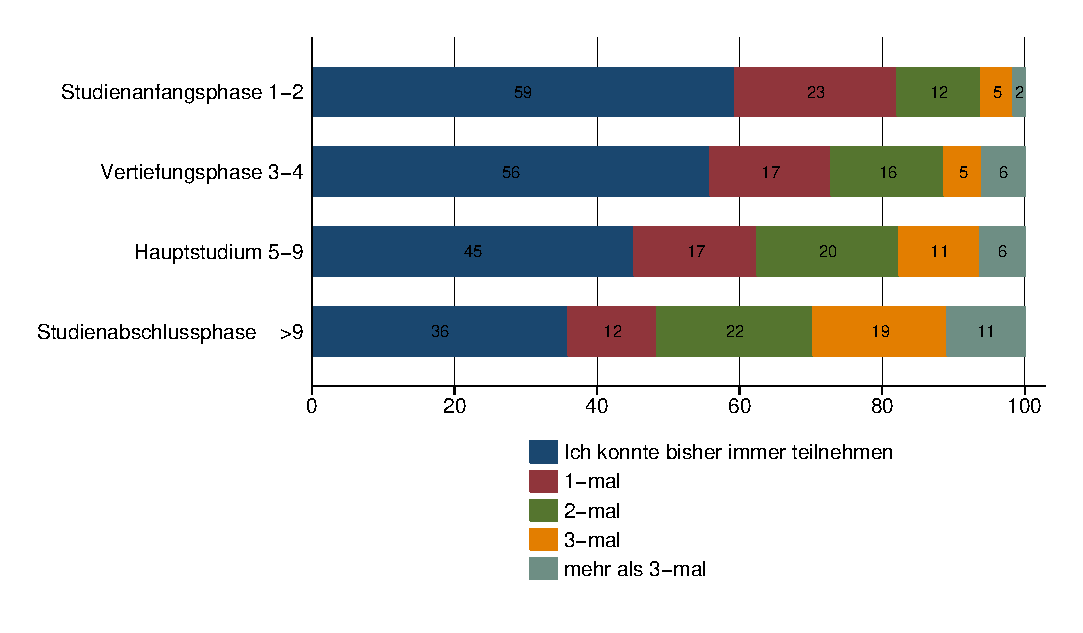
\includegraphics[
%  defaultresolution=72 !,
%  bmpsizefast=false
%]{image}
%\end{verbatim}
% \end{quote}
%
% \subsubsection{Hints}
%
% \begin{itemize}
% \item My version of \xfile{dvips.def} 1999/02/16 v3.0i defines
%       rules for the supported bitmap extensions, but does not
%       include them in the list of extensions that are tried
%       if the file name is not given with an extension.
%       In such a case, the list of extensions can be set
%       by \cs{DeclareGraphicsExtensions}, see \xpackage{grfguide}.
%       The following code just extends the list:
%       \begin{quote}
%\begin{verbatim}
%\makeatletter
%\g@addto@macro\Gin@extensions{,.bmp,.pcx,.msp}
%\makeatother
%\end{verbatim}
%       \end{quote}
% \item My version of \xfile{dvipdfm.def} 1998/11/24 vx.x misses
%       the graphics rule for PNG files. It can be added by:
%       \begin{quote}
%\begin{verbatim}
%\DeclareGraphicsRule{.png}{bmp}{.bb}{#1}
%\end{verbatim}
%       \end{quote}
%       See the previous issue to add the extension \xfile{.png} to the list
%       of extensions for package \xpackage{graphics}.
% \end{itemize}
%
% \subsubsection{Test program}
%
% There is a test program \xfile{bmpsize-test.tex}. Run it through
% \verb|latex|, \verb|pdflatex|, or \verb|pdftex|. Then given
% image files are inspected and the result is printed.
%
% \subsubsection{Interface for programmers}
%
% The macro names of the parsers are \verb|\bmpsize@read@|\meta{type}.
% Example: \cs{bmpsize@read@jpg} in case of JPEG.
%
% A parser sets the switch \cs{ifbmpsize@ok} to true, if it
% could successfully parse the image file.
% The width and height are returnd in \cs{bmpsize@width} and
% \cs{bmpsize@height}. If information about density is available,
% it is used to calculate width and height of the image, otherwise
% the values given by option \xoption{defaultresolution} is used.
% \xoption{resolution} overwrites the values in the image file.
%
% \subsection{Improved bitmap inclusion}
%
% Some drivers for package \xpackage{graphics} define the graphics
% type \xoption{bmp} for bitmap images. The code in the standard
% drivers for \xoption{dvips}, \xoption{dvipdfm}, and \xoption{dvipdfmx}
% is very basic and misses essential features of the
% package \xpackage{graphicx}. Therefore the code for bitmap
% inclusion is automatically rewritten by this package to add
% the following features:
% \begin{itemize}
% \item Support for \xoption{viewport} and \xoption{trim}.
% \item Support for \xoption{clip}.
% \item In case of \xoption{dvipdfm} and \xoption{dvipdfmx} the
%       bitmap images are reused and not included again if they
%       are used more than once.
% \end{itemize}
% However, there is a difference between \xoption{dvipdfm} and
% \xoption{dvipdfmx}, especially if images are reused. In the
% former case the reused box has width and height of 1bp, in the
% latter case its natural width. Thus the correct driver option must be given.
% \xoption{dvipdfm} and \xoption{dvipdfmx} are not equivalent.
%
% Older versions of \xoption{dvipdfmx} uses a size of 1in. However I do
% want to distinguish between versions of the same program. Therefore the
% support of these older versions has stopped with version 1.6 of this package.
% Use version dvipdfmx-20090708 or newer (some few versions before will
% probably also work, but I don't want to investigate this further).
%
% \StopEventually{
% }
%
% \section{Implementation}
%
% \subsection{Basic package \xpackage{bmpsize-base}}
%
%    Identification.
%    \begin{macrocode}
%<*base>
\ProvidesPackage{bmpsize-base}%
  [2009/09/04 v1.6 Basic part of bmpsize (HO)]%
%    \end{macrocode}
%    Modules of package \xpackage{fp} are used for calculations.
%    \begin{macrocode}
\RequirePackage{fp-basic}
\RequirePackage{fp-snap}
%    \end{macrocode}
%    Package \xpackage{fp} uses nested \cs{loop} structures.
%    That breaks with the plain-\TeX\ version of \cs{loop}.
%    Therefore we use the \LaTeX\ variant.
%    \begin{macro}{\@bmpsize@plain@loop}
%    \begin{macrocode}
\long\def\@bmpsize@plain@loop#1\repeat{%
  \def\iterate{%
    #1\relax
    \expandafter\iterate\fi
  }%
  \iterate
  \let\iterate\relax
}
%    \end{macrocode}
%    \end{macro}
%    \begin{macrocode}
\RequirePackage{pdftexcmds}[2007/11/11]
%    \end{macrocode}
%    \begin{macrocode}
\newif\ifbmpsize@ok
\let\@bmpsize@ok\bmpsize@oktrue

\newif\if@bmpsize@bigendian
\newif\if@bmpsize@absnum
\newif\if@bmpsize@user@resolution
\newif\if@bmpsize@fast
\@bmpsize@fasttrue

\def\@bmpsize@init{%
  \let\@bmpsize@org@plain@loop\loop
  \let\loop\@bmpsize@plain@loop
  \bmpsize@okfalse
  \@bmpsize@bigendiantrue
  \@bmpsize@absnumfalse
  \let\bmpsize@pixelwidth\relax
  \let\bmpsize@pixelheight\relax
  \let\bmpsize@pixelx\relax
  \let\bmpsize@pixely\relax
  \let\bmpsize@unit\relax
  \let\bmpsize@pixelxdenom\relax
  \let\bmpsize@pixelydenom\relax
  \let\bmpsize@orientation\relax
}

\def\@bmpsize@stop#1\@nil{}

\def\@bmpsize@loop#1{%
  #1%
  \@bmpsize@loop{#1}%
}
\def\@bmpsize@break#1\@bmpsize@loop#2{}

\def\@bmpsize@size#1#2#3{%
  \edef#3{\pdf@filesize{#1}}%
  \ifx#3\@empty
    \expandafter\@bmpsize@stop
  \fi
  \ifnum#3<#2\relax
    \expandafter\@bmpsize@stop
  \fi
}

\def\@bmpsize@read#1#2#3{%
  \edef\@bmpsize@buf{\pdf@filedump{#3}{#2}{#1}}%
  \edef\@bmpsize@temp{%
    \noexpand\@bmpsize@check@byte{#2}\@bmpsize@buf{}{}\noexpand\\%
  }%
  \@bmpsize@temp
}
\def\@bmpsize@fillbuf#1{%
  \ifx\@bmpsize@buf\@empty
    \expandafter\@firstofone
  \else
    \expandafter\@gobble
  \fi
  {%
    \edef\@bmpsize@buf{%
      \pdf@filedump{\bmpsize@offset}{\bmpsize@fillbuflength}{#1}%
    }%
    \ifx\@bmpsize@buf\@empty
      \expandafter\@bmpsize@stop
    \fi
    \edef\bmpsize@offset{\the\numexpr\bmpsize@offset+\bmpsize@fillbuflength}%
  }%
}
\def\bmpsize@fillbuflength{10}

\def\@bmpsize@append#1#2#3{%
  \edef#1{#2#3}%
}
\def\@bmpsize@pushback#1{%
  \edef\@bmpsize@buf{#1\@bmpsize@buf}%
}

\def\@bmpsize@iswhite#1{%
  \ifnum\pdf@strcmp{#1}{09}=\z@
  \else
    \ifnum\pdf@strcmp{#1}{0A}=\z@
    \else
      \ifnum\pdf@strcmp{#1}{0D}=\z@
      \else
        \ifnum\pdf@strcmp{#1}{20}=\z@
        \else
          1%
        \fi
      \fi
    \fi
  \fi
  \space
}
\def\@bmpsize@isdigit#1{%
  \ifnum\pdf@strcmp{#1}{30}<\z@
    1%
  \else
    \ifnum\pdf@strcmp{#1}{39}>\z@
      1%
    \fi
  \fi
  \space
}

\def\@bmpsize@check@byte#1#2#3{%
  \ifnum#1<\@ne
    \csname fi\endcsname
    \@bmpsize@cleanup@end
  \else
    \csname fi\endcsname
  \ifx!#2#3!%
    \csname fi\endcsname
    \@bmpsize@stop
  \else
    \csname fi\endcsname
    \expandafter\@bmpsize@check@byte\expandafter{\the\numexpr#1-1}%
}
\def\@bmpsize@cleanup@end#1\\{}

\def\@bmpsize@swap@maybe#1{%
  \if@bmpsize@bigendian
  \else
    \edef#1{\expandafter\@bmpsize@@swap#1\@empty\@empty\@empty\@empty}%
  \fi
}
\def\@bmpsize@@swap#1#2#3#4#5#6#7#8{%
  #7#8#5#6#3#4#1#2%
}

\def\@bmpsize@skip@one{%
  \edef\@bmpsize@buf{\expandafter\@gobbletwo\@bmpsize@buf}%
}
\def\@bmpsize@skip@two{%
  \edef\@bmpsize@buf{\expandafter\@gobblefour\@bmpsize@buf}%
}
\def\@bmpsize@skip@four{%
  \edef\@bmpsize@buf{%
    \expandafter\expandafter\expandafter\@gobblefour\expandafter
    \@gobblefour\@bmpsize@buf
  }%
}

\def\@bmpsize@grab#1#2{%
  \edef#1{\noexpand\@bmpsize@grab@byte#2=\@bmpsize@buf\noexpand\\}%
  \edef#1{#1}%
}
\def\@bmpsize@grab@byte#1=#2#3{%
  #2#3%
  \ifnum#1>\@ne
    \expandafter\@bmpsize@grab@byte\the\numexpr#1-1\expandafter=%
  \else
    \expandafter\@bmpsize@cleanup@end
  \fi
}

\def\@bmpsize@abs@maybe#1{%
  \let\@bmpsize@temp\relax
  \if@bmpsize@absnum
    \ifnum"\expandafter\@car#1\@nil>7 %
      \edef#1{\expandafter\@bmpsize@abs@byte#1\relax}%
      \ifnum\pdf@strcmp{#1}{7FFFFFFF}=\z@
        \let\@bmpsize@temp\@bmpsize@stop
      \else
        \def\@bmpsize@temp{\edef#1{\the\numexpr#1+1}}%
      \fi
    \fi
  \fi
}
\def\@bmpsize@abs@byte#1{%
  \ifx#1\relax
  \else
    \ifcase"0#1 %
      F\or E\or D\or C\or B\or A\or 9\or 8\or
      7\or 6\or 5\or 4\or 3\or 2\or 1\or 0%
    \fi
    \expandafter\@bmpsize@abs@byte
  \fi
}

\def\@bmpsize@num@one#1{%
  \@bmpsize@grab#11%
  \@bmpsize@abs@maybe#1%
  \edef#1{\number"#1}%
  \@bmpsize@temp
  \@bmpsize@skip@one
}
\def\@bmpsize@num@two#1{%
  \@bmpsize@grab#12%
  \@bmpsize@swap@maybe#1%
  \@bmpsize@abs@maybe#1%
  \edef#1{\number"#1}%
  \@bmpsize@temp
  \@bmpsize@skip@two
}
\def\@bmpsize@num@four#1{%
  \@bmpsize@grab#14%
  \@bmpsize@swap@maybe#1%
  \@bmpsize@abs@maybe#1%
  \ifnum\pdf@strcmp{#1}{7FFFFFFF}>\z@
    \expandafter\@bmpsize@stop
  \fi
  \edef#1{\number"#1}%
  \@bmpsize@temp
  \@bmpsize@skip@four
}

\def\@bmpsize@div#1#2#3{% #1 := #2/#3
  \FPdiv#1{#2}{#3}%
  \@bmpsize@beautify#1%
}
\def\@bmpsize@beautify#1{%
  \FPifint#1%
    \edef#1{\expandafter\@bmpsize@trunc#1.\@nil}%
  \else
    \edef#1{\expandafter\@bmpsize@cleanup@frac#1.\@nil}%
  \fi
}
\def\@bmpsize@trunc#1.#2\@nil{#1}
% #1 isn't an integer, thus we should have at least one
% necessary digit after the dot
\def\@bmpsize@cleanup@frac#1.#2#3.#4\@nil{%
  #1.#2%
  \ifx\\#3\\%
  \else
    \@bmpsize@cleanup@fracdigits#3000000000\@nil
  \fi
}
\def\@bmpsize@cleanup@fracdigits#1#2#3#4#5#6#7#8#9{%
  \ifcase#9 %
    \ifcase#8 %
      \ifcase#7 %
        \ifcase#6 %
          \ifcase#5 %
            \ifcase #4 %
              \ifcase #3 %
                \ifcase #2 %
                  \ifcase #1 %
                  \else
                    #1%
                  \fi
                \else
                  #1#2%
                \fi
              \else
                #1#2#3%
              \fi
            \else
              #1#2#3#4%
            \fi
          \else
            #1#2#3#4#5%
          \fi
        \else
          #1#2#3#4#5#6%
        \fi
      \else
        #1#2#3#4#5#6#7%
      \fi
    \else
      #1#2#3#4#5#6#7#8%
    \fi
  \else
    #1#2#3#4#5#6#7#8#9%
  \fi
  \@bmpsize@trunc.%
}

\def\@bmpsize@end{%
  \ifbmpsize@ok
    \ifx\bmpsize@pixelwidth\relax
      \bmpsize@okfalse
    \fi
    \ifx\bmpsize@pixelheight\relax
      \bmpsize@okfalse
    \fi
  \fi
  \ifbmpsize@ok
    \ifnum\bmpsize@pixelwidth>\z@
    \else
      \bmpsize@okfalse
    \fi
    \ifnum\bmpsize@pixelheight>\z@
    \else
      \bmpsize@okfalse
    \fi
  \fi
  \ifbmpsize@ok
    \ifcase 0%
      \ifx\bmpsize@pixelx\relax 1 \fi
      \ifx\bmpsize@pixely\relax 1 \fi
      \ifnum\bmpsize@pixelx>\z@\else 1 \fi
      \ifnum\bmpsize@pixely>\z@\else 1 \fi
      \ifx\bmpsize@pixelxdenom\relax
         \ifx\bmpsize@pixelydenom\relax\else 1 \fi
      \else
        \ifnum\bmpsize@pixelxdenom>\z@\else 1 \fi
      \fi
      \ifx\bmpsize@pixelydenom\relax
      \else
        \ifnum\bmpsize@pixelydenom>\z@\else 1 \fi
      \fi
    \else
      \let\bmpsize@pixelx\relax
      \let\bmpsize@pixely\relax
      \let\bmpsize@unit\relax
      \let\bmpsize@pixelxdenom\relax
      \let\bmpsize@pixelydenom\relax
    \fi
    \ifx\bmpsize@pixelxdenom\relax
    \else
      \@bmpsize@div\bmpsize@pixelx\bmpsize@pixelx\bmpsize@pixelxdenom
      \@bmpsize@div\bmpsize@pixely\bmpsize@pixely\bmpsize@pixelydenom
      \let\bmpsize@pixelxdenom\relax
      \let\bmpsize@pixelydenom\relax
    \fi
    \ifcase 0\ifx\bmpsize@unit\relax 1\fi
             \if@bmpsize@user@resolution 1\fi
             \relax
      \let\bmpsize@calc@unit\bmpsize@unit
      \let\bmpsize@calc@pixelx\bmpsize@pixelx
      \let\bmpsize@calc@pixely\bmpsize@pixely
    \else
      \let\bmpsize@calc@unit\bmpsize@unit@default
      \let\bmpsize@calc@pixelx\bmpsize@pixelx@default
      \let\bmpsize@calc@pixely\bmpsize@pixely@default
      \ifx\bmpsize@calc@pixely\Gin@exclamation
        \ifx\bmpsize@pixelx\relax
          \let\bmpsize@calc@pixely\bmpsize@calc@pixelx
        \else
          \FPdiv\bmpsize@calc@pixely\bmpsize@calc@pixelx\bmpsize@pixelx
          \FPmul\bmpsize@calc@pixely\bmpsize@calc@pixely\bmpsize@pixely
        \fi
      \else
        \ifx\bmpsize@calc@pixelx\Gin@exclamation
          \ifx\bmpsize@pixelx\relax
            \let\bmpsize@calc@pixelx\bmpsize@calc@pixely
          \else
            \FPdiv\bmpsize@calc@pixelx\bmpsize@calc@pixely\bmpsize@pixely
            \FPmul\bmpsize@calc@pixelx\bmpsize@calc@pixelx\bmpsize@pixelx
          \fi
        \fi
      \fi
    \fi
    \FPdiv\bmpsize@width\bmpsize@pixelwidth\bmpsize@calc@pixelx
    \FPdiv\bmpsize@height\bmpsize@pixelheight\bmpsize@calc@pixely
    % calculation of width and height in bp for package graphics
    % 1in = 72bp = 72.27pt, 72/72.27 = 8/8.03, 1pt = 65536sp
    \if@bmpsize@fast
      \edef\bmpsize@width{%
        \strip@pt\dimexpr.99626\dimexpr
        \bmpsize@width\dimexpr\bmpsize@calc@unit
      }%
      \edef\bmpsize@height{%
        \strip@pt\dimexpr.99626\dimexpr
        \bmpsize@height\dimexpr\bmpsize@calc@unit
      }%
    \else
      \edef\@bmpsize@temp{\number\dimexpr\bmpsize@calc@unit}%
      \ifnum\@bmpsize@temp>100000 %
        \FPmul\@bmpsize@temp\@bmpsize@temp{0.00001}%
        \def\@bmpsize@corr{100000}%
      \else
        \let\@bmpsize@corr\relax
      \fi
      \FPmul\bmpsize@width\bmpsize@width\@bmpsize@temp
      \FPmul\bmpsize@height\bmpsize@height\@bmpsize@temp
      \FPmul\bmpsize@width\bmpsize@width{8}%
      \FPmul\bmpsize@height\bmpsize@height{8}%
      \FPdiv\bmpsize@width\bmpsize@width{8.03}%
      \FPdiv\bmpsize@height\bmpsize@height{8.03}%
      \FPdiv\bmpsize@width\bmpsize@width{65536}%
      \FPdiv\bmpsize@height\bmpsize@height{65536}%
      \ifx\@bmpsize@corr\relax
      \else
        \FPmul\bmpsize@width\bmpsize@width\@bmpsize@corr
        \FPmul\bmpsize@height\bmpsize@height\@bmpsize@corr
      \fi
      \FPround\bmpsize@width\bmpsize@width{5}%
      \FPround\bmpsize@height\bmpsize@height{5}%
      \@bmpsize@beautify\bmpsize@width
      \@bmpsize@beautify\bmpsize@height
    \fi
  \fi
  \let\loop\@bmpsize@org@plain@loop
}
\def\bmpsize@unit@default{72.27pt}% more accurate than 1in
\def\bmpsize@pixelx@default{72}
\let\bmpsize@pixely@default\Gin@exclamation

\def\bmpsize@types{png,jpg,bmp,gif,tiff,pnm,pam,xpm,tga,pcx,msp,sgi}
%</base>
%    \end{macrocode}
%
% \subsection{Bitmap formats}
%
% \subsubsection{png}
%
%\iffalse
%<*ignore>
%\fi
%\begin{verbatim}
%begin png
%big-endian
%
%read 24 0
%grab 8        -> $temp
%check streq $temp [0x89 "PNG" 0x0D 0x0A 0x1A 0x0A]
%num 4         -> $length
%grab 4        -> $temp
%check streq $temp ["IHDR"]
%num 4         -> $pixelwidth
%num 4         -> $pixelheight
%ok
%assign numexpr(20 + $length) -> $offset
%loop
%  read 8 $offset
%  num 4       -> $length
%  grab 4      -> $temp
%  if streq $temp ["IDAT"]
%    stop
%  fi
%  if streq $temp ["pHYs"]
%    read 9 numexpr($offset + 8)
%    num 4     -> $pixelx
%    num 4     -> $pixely
%    grab 1     -> $temp
%    if numeq $temp 1
%      assign {100cm} -> $unit
%    fi
%    stop
%  fi
%  assign numexpr($offset + 12 + $length) -> $offset
%repeat
%end
%\end{verbatim}
%\iffalse
%</ignore>
%\fi
%    \begin{macro}{\bmpsize@read@png}
%    \begin{macrocode}
%<*base>
\def\bmpsize@read@png#1{%
  \@bmpsize@init
  \@bmpsize@bigendiantrue
  \@bmpsize@read{#1}{24}{0}%
  \@bmpsize@grab\bmpsize@temp{8}%
  \@bmpsize@skip@four
  \@bmpsize@skip@four
  \ifnum\pdf@strcmp{\bmpsize@temp}{89504E470D0A1A0A}=\z@
  \else
    \expandafter\@bmpsize@stop
  \fi
  \@bmpsize@num@four\bmpsize@length
  \@bmpsize@grab\bmpsize@temp{4}%
  \@bmpsize@skip@four
  \ifnum\pdf@strcmp{\bmpsize@temp}{49484452}=\z@
  \else
    \expandafter\@bmpsize@stop
  \fi
  \@bmpsize@num@four\bmpsize@pixelwidth
  \@bmpsize@num@four\bmpsize@pixelheight
  \@bmpsize@ok
  \edef\bmpsize@offset{\the\numexpr20+\bmpsize@length}%
  \@bmpsize@loop{%
    \@bmpsize@read{#1}{8}{\bmpsize@offset}%
    \@bmpsize@num@four\bmpsize@length
    \@bmpsize@grab\bmpsize@temp{4}%
    \@bmpsize@skip@four
    \ifnum\pdf@strcmp{\bmpsize@temp}{49444154}=\z@
      \expandafter\@firstofone
    \else
      \expandafter\@gobble
    \fi
    {%
      \@bmpsize@stop
    }%
    \ifnum\pdf@strcmp{\bmpsize@temp}{70485973}=\z@
      \expandafter\@firstofone
    \else
      \expandafter\@gobble
    \fi
    {%
      \@bmpsize@read{#1}{9}{\numexpr\bmpsize@offset+8\relax}%
      \@bmpsize@num@four\bmpsize@pixelx
      \@bmpsize@num@four\bmpsize@pixely
      \@bmpsize@grab\bmpsize@temp{1}%
      \@bmpsize@skip@one
      \ifnum\bmpsize@temp=1\relax
        \expandafter\@firstofone
      \else
        \expandafter\@gobble
      \fi
      {%
        \def\bmpsize@unit{100cm}%
      }%
      \@bmpsize@stop
    }%
    \edef\bmpsize@offset{\the\numexpr\bmpsize@offset+12+\bmpsize@length}%
  }%
  \@bmpsize@stop
  \@nil
  \@bmpsize@end
}%
%</base>
%    \end{macrocode}
%    \end{macro}
%
% \subsubsection{jpg}
%
%\iffalse
%<*ignore>
%\fi
%\begin{verbatim}
%begin jpg
%
%read 3 0
%grab 3      -> $temp % SOI and 0xFF
%check streq $temp [0xFF 0xD8 0xFF]
%assign {2} -> $offset
%assign {0} -> $exifdensity
%loop
%  read 4 $offset
%  grab 1    -> $temp
%  check streq $temp [0xFF]
%  num 1    -> $temp
%  if numeq $temp 0xDA % SOS
%    stop
%  fi
%  % look for JFIF APP0 segment
%  if numeq $temp 0xE0 % APP0
%    num 2       -> $length
%    if numeq $exifdensity 0
%      if numge $length 16 % a JFIF segment has 16 bytes at least
%        read 12 numexpr($offset + 4)
%        grab 5      -> $temp % identifier
%        if streq $temp ["JFIF" 0x0]
%          check numge $length 16
%          skip 2 % version
%          num 1       -> $temp % units
%          if numeq $temp 1
%            assign {72.27pt} -> $unit
%          else
%            if numeq $temp 2
%              assign {1cm} -> $unit
%            fi
%          fi
%          num 2    -> $pixelx
%          num 2    -> $pixely
%        fi
%      fi
%    fi
%  else
%    if numeq $temp 0xE1 % APP1
%      % look for Exif APP1 segment
%      num 2 -> $length
%      if numge $length 20 % identifier (6) + Tiff header (8) + first IFD (>=6)
%        read 20 numexpr($offset + 4)
%        grab 6 -> $temp
%        if streq $temp ["Exif" 0x0 0x0]
%          assign numexpr($offset + 10) -> $exifoffset
%          % read TIFF header
%          grab 2 -> $temp
%          if streq $temp ["II"]
%            little-endian
%          else
%            check streq $temp ["MM"]
%            % big-endian
%          fi
%          num 2 -> $temp
%          check numeq $temp 42
%          num 4 -> $temp % offset of first IFD
%          check numgt $temp 0
%          % read first IFD
%          assign numexpr($temp + $exifoffset) -> $off
%          read 2 $off
%          num 2 -> $entries
%          assign numexpr($off + 2) -> $off
%          loop
%            if numeq $entries 0
%              break
%            fi
%            assign numexpr($entries - 1) -> $entries
%            % entry format:
%            % 2 tag
%            % 2 field type
%            % 4 count
%            % 4 value/offset
%            read 12 $off
%            assign numexpr($off + 12) -> $off
%            num 2 -> $tag
%            if numeq $tag 296 % ResolutionUnit
%              skip 6 % type: 3 (short), count: 1
%              num 2 -> $temp
%              ifcase $temp
%              or % 1
%                clear $unit
%              or % 2
%                assign {72.27pt} -> $unit
%              or % 3
%                assign {1cm} -> $unit
%              else
%                clear $unit % unknown
%              fi
%              ifcase $temp
%              or % 1
%              or % 2
%                assign {1} -> $exifdensity
%              or % 3
%                assign {1} -> $exifdensity
%              else
%                assign $exifdensity -> $exifdensity
%              fi
%            fi
%            % 256 ImageWidth (use width of JPG part)
%            % 257 ImageHeight (use height of JPG part)
%            if numeq $tag 274 % Orientation
%              skip 6 % type: 3 (short), count: 1
%              num 2 -> $temp
%              if numge $temp 0 
%                if numle $temp 8
%                  assign $temp -> $orientation
%                fi
%              fi
%            fi
%            if numeq $tag 282 % XResolution
%              skip 6
%              num 4 -> $temp
%              read 8 numexpr($temp + $exifoffset)
%              num 4 -> $pixelx
%              num 4 -> $temp
%              if numeq $temp 1
%              else
%                assign numexpr($temp) -> $pixelxdenom
%                % div $pixelx $temp -> $pixelx
%              fi
%            fi
%            if numeq $tag 283 % YResolution
%              skip 6
%              num 4 -> $temp
%              read 8 numexpr($temp + $exifoffset)
%              num 4 -> $pixely
%              num 4 -> $temp
%              if numeq $temp 1
%              else
%                assign numexpr($temp) -> $pixelydenom
%                % div $pixely $temp -> $pixely
%              fi
%            fi
%          repeat
%          big-endian
%        fi
%      fi
%    else
%      assign numexpr($temp - 0xC0) -> $temp
%      ifcase $temp % SOF_0
%      or % SOF_1
%      or % SOF_2
%      or % SOF_3
%      or % DHT
%        assign {-1} -> $temp
%      or % SOF_5
%      or % SOF_6
%      or % SOF_7
%      or % JPG
%        assign {-1} -> $temp
%      or % SOF_9
%      or % SOF_10
%      or % SOF_11
%      or % DAC
%        assign {-1} -> $temp
%      or % SOF_13
%      or % SOF_14
%      or % SOF_15
%      else
%        assign {-1} -> $temp
%      fi
%      if numeq $temp -1
%      else
%        read 4 numexpr($offset + 5)
%        num 2  -> $pixelheight
%        num 2  -> $pixelwidth
%        if numeq $pixelheight 0
%          clear $pixelheight
%          stop
%        fi
%        ok
%        stop
%      fi
%      num 2 -> $length
%    fi
%  fi
%  assign numexpr($offset + $length + 2) -> $offset
%repeat
%end
%\end{verbatim}
%\iffalse
%</ignore>
%\fi
%    \begin{macro}{\bmpsize@read@jpg}
%    \begin{macrocode}
%<*base>
\def\bmpsize@read@jpg#1{%
  \@bmpsize@init
  \@bmpsize@read{#1}{3}{0}%
  \@bmpsize@grab\bmpsize@temp{3}%
  \@bmpsize@skip@two
  \@bmpsize@skip@one
  \ifnum\pdf@strcmp{\bmpsize@temp}{FFD8FF}=\z@
  \else
    \expandafter\@bmpsize@stop
  \fi
  \def\bmpsize@offset{2}%
  \def\bmpsize@exifdensity{0}%
  \@bmpsize@loop{%
    \@bmpsize@read{#1}{4}{\bmpsize@offset}%
    \@bmpsize@grab\bmpsize@temp{1}%
    \@bmpsize@skip@one
    \ifnum\pdf@strcmp{\bmpsize@temp}{FF}=\z@
    \else
      \expandafter\@bmpsize@stop
    \fi
    \@bmpsize@num@one\bmpsize@temp
    \ifnum\bmpsize@temp=218\relax
      \expandafter\@firstofone
    \else
      \expandafter\@gobble
    \fi
    {%
      \@bmpsize@stop
    }%
    \ifnum\bmpsize@temp=224\relax
      \expandafter\@firstoftwo
    \else
      \expandafter\@secondoftwo
    \fi
    {%
      \@bmpsize@num@two\bmpsize@length
      \ifnum\bmpsize@exifdensity=0\relax
        \expandafter\@firstofone
      \else
        \expandafter\@gobble
      \fi
      {%
        \unless\ifnum\bmpsize@length<16\relax
          \expandafter\@firstofone
        \else
          \expandafter\@gobble
        \fi
        {%
          \@bmpsize@read{#1}{12}{\numexpr\bmpsize@offset+4\relax}%
          \@bmpsize@grab\bmpsize@temp{5}%
          \@bmpsize@skip@four
          \@bmpsize@skip@one
          \ifnum\pdf@strcmp{\bmpsize@temp}{4A46494600}=\z@
            \expandafter\@firstofone
          \else
            \expandafter\@gobble
          \fi
          {%
            \ifnum\bmpsize@length<16\relax
              \expandafter\@bmpsize@stop
            \fi
            \@bmpsize@skip@two
            \@bmpsize@num@one\bmpsize@temp
            \ifnum\bmpsize@temp=1\relax
              \expandafter\@firstoftwo
            \else
              \expandafter\@secondoftwo
            \fi
            {%
              \def\bmpsize@unit{72.27pt}%
            }{%
              \ifnum\bmpsize@temp=2\relax
                \expandafter\@firstofone
              \else
                \expandafter\@gobble
              \fi
              {%
                \def\bmpsize@unit{1cm}%
              }%
            }%
            \@bmpsize@num@two\bmpsize@pixelx
            \@bmpsize@num@two\bmpsize@pixely
          }%
        }%
      }%
    }{%
      \ifnum\bmpsize@temp=225\relax
        \expandafter\@firstoftwo
      \else
        \expandafter\@secondoftwo
      \fi
      {%
        \@bmpsize@num@two\bmpsize@length
        \unless\ifnum\bmpsize@length<20\relax
          \expandafter\@firstofone
        \else
          \expandafter\@gobble
        \fi
        {%
          \@bmpsize@read{#1}{20}{\numexpr\bmpsize@offset+4\relax}%
          \@bmpsize@grab\bmpsize@temp{6}%
          \@bmpsize@skip@four
          \@bmpsize@skip@two
          \ifnum\pdf@strcmp{\bmpsize@temp}{457869660000}=\z@
            \expandafter\@firstofone
          \else
            \expandafter\@gobble
          \fi
          {%
            \edef\bmpsize@exifoffset{\the\numexpr\bmpsize@offset+10}%
            \@bmpsize@grab\bmpsize@temp{2}%
            \@bmpsize@skip@two
            \ifnum\pdf@strcmp{\bmpsize@temp}{4949}=\z@
              \expandafter\@firstoftwo
            \else
              \expandafter\@secondoftwo
            \fi
            {%
              \@bmpsize@bigendianfalse
            }{%
              \ifnum\pdf@strcmp{\bmpsize@temp}{4D4D}=\z@
              \else
                \expandafter\@bmpsize@stop
              \fi
            }%
            \@bmpsize@num@two\bmpsize@temp
            \ifnum\bmpsize@temp=42\relax
            \else
              \expandafter\@bmpsize@stop
            \fi
            \@bmpsize@num@four\bmpsize@temp
            \ifnum\bmpsize@temp>0\relax
            \else
              \expandafter\@bmpsize@stop
            \fi
            \edef\bmpsize@off{\the\numexpr\bmpsize@temp+\bmpsize@exifoffset}%
            \@bmpsize@read{#1}{2}{\bmpsize@off}%
            \@bmpsize@num@two\bmpsize@entries
            \edef\bmpsize@off{\the\numexpr\bmpsize@off+2}%
            \@bmpsize@loop{%
              \ifnum\bmpsize@entries=0\relax
                \expandafter\@firstofone
              \else
                \expandafter\@gobble
              \fi
              {%
                \@bmpsize@break
              }%
              \edef\bmpsize@entries{\the\numexpr\bmpsize@entries-1}%
              \@bmpsize@read{#1}{12}{\bmpsize@off}%
              \edef\bmpsize@off{\the\numexpr\bmpsize@off+12}%
              \@bmpsize@num@two\bmpsize@tag
              \ifnum\bmpsize@tag=296\relax
                \expandafter\@firstofone
              \else
                \expandafter\@gobble
              \fi
              {%
                \@bmpsize@skip@four
                \@bmpsize@skip@two
                \@bmpsize@num@two\bmpsize@temp
                \ifcase\bmpsize@temp\relax
                \or
                  \let\bmpsize@unit\relax
                \or
                  \def\bmpsize@unit{72.27pt}%
                \or
                  \def\bmpsize@unit{1cm}%
                \else
                  \let\bmpsize@unit\relax
                \fi
                \ifcase\bmpsize@temp\relax
                \or
                \or
                  \def\bmpsize@exifdensity{1}%
                \or
                  \def\bmpsize@exifdensity{1}%
                \else
                  \let\bmpsize@exifdensity\bmpsize@exifdensity
                \fi
              }%
              \ifnum\bmpsize@tag=274\relax
                \expandafter\@firstofone
              \else
                \expandafter\@gobble
              \fi
              {%
                \@bmpsize@skip@four
                \@bmpsize@skip@two
                \@bmpsize@num@two\bmpsize@temp
                \unless\ifnum\bmpsize@temp<0\relax
                  \expandafter\@firstofone
                \else
                  \expandafter\@gobble
                \fi
                {%
                  \unless\ifnum\bmpsize@temp>8\relax
                    \expandafter\@firstofone
                  \else
                    \expandafter\@gobble
                  \fi
                  {%
                    \let\bmpsize@orientation\bmpsize@temp
                  }%
                }%
              }%
              \ifnum\bmpsize@tag=282\relax
                \expandafter\@firstofone
              \else
                \expandafter\@gobble
              \fi
              {%
                \@bmpsize@skip@four
                \@bmpsize@skip@two
                \@bmpsize@num@four\bmpsize@temp
                \@bmpsize@read{#1}{8}{\numexpr\bmpsize@temp+\bmpsize@exifoffset\relax}%
                \@bmpsize@num@four\bmpsize@pixelx
                \@bmpsize@num@four\bmpsize@temp
                \ifnum\bmpsize@temp=1\relax
                  \expandafter\@gobble
                \else
                  \expandafter\@firstofone
                \fi
                {%
                  \edef\bmpsize@pixelxdenom{\the\numexpr\bmpsize@temp}%
                }%
              }%
              \ifnum\bmpsize@tag=283\relax
                \expandafter\@firstofone
              \else
                \expandafter\@gobble
              \fi
              {%
                \@bmpsize@skip@four
                \@bmpsize@skip@two
                \@bmpsize@num@four\bmpsize@temp
                \@bmpsize@read{#1}{8}{\numexpr\bmpsize@temp+\bmpsize@exifoffset\relax}%
                \@bmpsize@num@four\bmpsize@pixely
                \@bmpsize@num@four\bmpsize@temp
                \ifnum\bmpsize@temp=1\relax
                  \expandafter\@gobble
                \else
                  \expandafter\@firstofone
                \fi
                {%
                  \edef\bmpsize@pixelydenom{\the\numexpr\bmpsize@temp}%
                }%
              }%
            }%
            \@bmpsize@bigendiantrue
          }%
        }%
      }{%
        \edef\bmpsize@temp{\the\numexpr\bmpsize@temp-192}%
        \ifcase\bmpsize@temp\relax
        \or
        \or
        \or
        \or
          \def\bmpsize@temp{-1}%
        \or
        \or
        \or
        \or
          \def\bmpsize@temp{-1}%
        \or
        \or
        \or
        \or
          \def\bmpsize@temp{-1}%
        \or
        \or
        \or
        \else
          \def\bmpsize@temp{-1}%
        \fi
        \ifnum\bmpsize@temp=-1\relax
          \expandafter\@gobble
        \else
          \expandafter\@firstofone
        \fi
        {%
          \@bmpsize@read{#1}{4}{\numexpr\bmpsize@offset+5\relax}%
          \@bmpsize@num@two\bmpsize@pixelheight
          \@bmpsize@num@two\bmpsize@pixelwidth
          \ifnum\bmpsize@pixelheight=0\relax
            \expandafter\@firstofone
          \else
            \expandafter\@gobble
          \fi
          {%
            \let\bmpsize@pixelheight\relax
            \@bmpsize@stop
          }%
          \@bmpsize@ok
          \@bmpsize@stop
        }%
        \@bmpsize@num@two\bmpsize@length
      }%
    }%
    \edef\bmpsize@offset{\the\numexpr\bmpsize@offset+\bmpsize@length+2}%
  }%
  \@bmpsize@stop
  \@nil
  \@bmpsize@end
}%
%</base>
%    \end{macrocode}
%    \end{macro}
%
% \subsubsection{bmp}
%
%\iffalse
%<*ignore>
%\fi
%\begin{verbatim}
%begin bmp
%little-endian
%
%read 26 0
%grab 2 -> $temp
%check streq $temp ["BM"]
%skip 12
%% header size is 4 bytes in V3+, unknown for V1, V2,
%% known header sizes fit in 2 bytes
%num 2   -> $temp
%if numeq $temp 12 % V1
%  skip 2
%  num 2 -> $pixelwidth
%  num 2 -> $pixelheight
%  % no resolution entries
%  ok
%  stop
%fi
%if numeq $temp 64 % V2
%  skip 2
%  num 2 -> $pixelwidth
%  num 2 -> $pixelheight
%  % missing specification for resolution
%  ok
%  stop
%fi
%% V3, V4, V5
%skip 2
%num 4 -> $pixelwidth
%absnum 4 -> $pixelheight
%ok
%read 8 38
%num 4 -> $pixelx
%num 4 -> $pixely
%assign {100cm} -> $unit
%end
%\end{verbatim}
%\iffalse
%</ignore>
%\fi
%    \begin{macro}{\bmpsize@read@bmp}
%    \begin{macrocode}
%<*base>
\def\bmpsize@read@bmp#1{%
  \@bmpsize@init
  \@bmpsize@bigendianfalse
  \@bmpsize@read{#1}{26}{0}%
  \@bmpsize@grab\bmpsize@temp{2}%
  \@bmpsize@skip@two
  \ifnum\pdf@strcmp{\bmpsize@temp}{424D}=\z@
  \else
    \expandafter\@bmpsize@stop
  \fi
  \@bmpsize@skip@four
  \@bmpsize@skip@four
  \@bmpsize@skip@four
  \@bmpsize@num@two\bmpsize@temp
  \ifnum\bmpsize@temp=12\relax
    \expandafter\@firstofone
  \else
    \expandafter\@gobble
  \fi
  {%
    \@bmpsize@skip@two
    \@bmpsize@num@two\bmpsize@pixelwidth
    \@bmpsize@num@two\bmpsize@pixelheight
    \@bmpsize@ok
    \@bmpsize@stop
  }%
  \ifnum\bmpsize@temp=64\relax
    \expandafter\@firstofone
  \else
    \expandafter\@gobble
  \fi
  {%
    \@bmpsize@skip@two
    \@bmpsize@num@two\bmpsize@pixelwidth
    \@bmpsize@num@two\bmpsize@pixelheight
    \@bmpsize@ok
    \@bmpsize@stop
  }%
  \@bmpsize@skip@two
  \@bmpsize@num@four\bmpsize@pixelwidth
  \@bmpsize@absnumtrue
  \@bmpsize@num@four\bmpsize@pixelheight
  \@bmpsize@absnumfalse
  \@bmpsize@ok
  \@bmpsize@read{#1}{8}{38}%
  \@bmpsize@num@four\bmpsize@pixelx
  \@bmpsize@num@four\bmpsize@pixely
  \def\bmpsize@unit{100cm}%
  \@bmpsize@stop
  \@nil
  \@bmpsize@end
}%
%</base>
%    \end{macrocode}
%    \end{macro}
%
% \subsubsection{gif}
%
%\iffalse
%<*ignore>
%\fi
%\begin{verbatim}
%begin gif
%little-endian
%
%% Header
%read 13 0
%grab 3      -> $temp
%check streq $temp ["GIF"]
%skip 3      % version
%
%% Logical Screen Descriptor
%num 2       -> $pixelwidth
%num 2       -> $pixelheight
%skip 2
%num 1       -> $temp % Pixel Aspect Ratio
%if numeq $temp 0
%else
%  assign numexpr($temp + 15) -> $pixelx
%  assign {64}     -> $pixely
%fi
%ok
%end
%\end{verbatim}
%\iffalse
%</ignore>
%\fi
%    \begin{macro}{\bmpsize@read@gif}
%    \begin{macrocode}
%<*base>
\def\bmpsize@read@gif#1{%
  \@bmpsize@init
  \@bmpsize@bigendianfalse
  \@bmpsize@read{#1}{13}{0}%
  \@bmpsize@grab\bmpsize@temp{3}%
  \@bmpsize@skip@two
  \@bmpsize@skip@one
  \ifnum\pdf@strcmp{\bmpsize@temp}{474946}=\z@
  \else
    \expandafter\@bmpsize@stop
  \fi
  \@bmpsize@skip@two
  \@bmpsize@skip@one
  \@bmpsize@num@two\bmpsize@pixelwidth
  \@bmpsize@num@two\bmpsize@pixelheight
  \@bmpsize@skip@two
  \@bmpsize@num@one\bmpsize@temp
  \ifnum\bmpsize@temp=0\relax
    \expandafter\@gobble
  \else
    \expandafter\@firstofone
  \fi
  {%
    \edef\bmpsize@pixelx{\the\numexpr\bmpsize@temp+15}%
    \def\bmpsize@pixely{64}%
  }%
  \@bmpsize@ok
  \@bmpsize@stop
  \@nil
  \@bmpsize@end
}%
%</base>
%    \end{macrocode}
%    \end{macro}
%
% \subsubsection{tiff}
%
%\iffalse
%<*ignore>
%\fi
%\begin{verbatim}
%begin tiff
%% defaults
%assign {72.27pt} -> $unit
%
%% Image File Header
%read 8 0
%grab 2 -> $temp
%if streq $temp ["II"]
%  little-endian
%else
%  check streq $temp ["MM"]
%  big-endian
%fi
%num 2 -> $temp
%check numeq $temp 42
%num 4 -> $offset % first IFD (Image File Directory)
%
%% First IFD
%read 2 $offset
%assign numexpr($offset + 2) -> $offset
%num 2 -> $entries
%ok % must rely on checks at the end
%loop
%  if numeq $entries 0
%    stop
%  fi
%  assign numexpr($entries - 1) -> $entries
%  % entry format:
%  % 2 tag
%  % 2 field type
%  % 4 count
%  % 4 value/offset
%  read 12 $offset
%  assign numexpr($offset + 12) -> $offset
%  num 2 -> $tag % tag
%  if numeq $temp 296 % ResolutionUnit
%    skip 6 % type: 3 (short), count: 1
%    num 2 -> $temp
%    ifcase $temp
%    or % 1
%      clear $unit
%    or % 2
%      assign {72.27pt} -> $unit
%    or % 3
%      assign {1cm} -> $unit
%    else
%      clear $unit
%    fi
%  fi
%  if numeq $tag 256 % ImageWidth
%    skip 6
%    num 4 -> $pixelwidth
%  fi
%  if numeq $tag 257 % ImageLength
%    skip 6
%    num 4 -> $pixelheight
%  fi
%  if numeq $tag 282 % XResolution
%    skip 6
%    num 4 -> $temp
%    read 8 $temp
%    num 4 -> $pixelx
%    num 4 -> $temp
%    if numeq $temp 1
%    else
%      assign numexpr($temp) -> $pixelxdenom
%      % div $pixelx $temp -> $pixelx
%    fi
%  fi
%  if numeq $tag 283 % YResolution
%    skip 6
%    num 4 -> $temp
%    read 8 $temp
%    num 4 -> $pixely
%    num 4 -> $temp
%    if numeq $temp 1
%    else
%      assign numexpr($temp) -> $pixelydenom
%      % div $pixely $temp -> $pixely
%    fi
%  fi
%repeat
%end
%\end{verbatim}
%\iffalse
%</ignore>
%\fi
%    \begin{macro}{\bmpsize@read@tiff}
%    \begin{macrocode}
%<*base>
\def\bmpsize@read@tiff#1{%
  \@bmpsize@init
  \def\bmpsize@unit{72.27pt}%
  \@bmpsize@read{#1}{8}{0}%
  \@bmpsize@grab\bmpsize@temp{2}%
  \@bmpsize@skip@two
  \ifnum\pdf@strcmp{\bmpsize@temp}{4949}=\z@
    \expandafter\@firstoftwo
  \else
    \expandafter\@secondoftwo
  \fi
  {%
    \@bmpsize@bigendianfalse
  }{%
    \ifnum\pdf@strcmp{\bmpsize@temp}{4D4D}=\z@
    \else
      \expandafter\@bmpsize@stop
    \fi
    \@bmpsize@bigendiantrue
  }%
  \@bmpsize@num@two\bmpsize@temp
  \ifnum\bmpsize@temp=42\relax
  \else
    \expandafter\@bmpsize@stop
  \fi
  \@bmpsize@num@four\bmpsize@offset
  \@bmpsize@read{#1}{2}{\bmpsize@offset}%
  \edef\bmpsize@offset{\the\numexpr\bmpsize@offset+2}%
  \@bmpsize@num@two\bmpsize@entries
  \@bmpsize@ok
  \@bmpsize@loop{%
    \ifnum\bmpsize@entries=0\relax
      \expandafter\@firstofone
    \else
      \expandafter\@gobble
    \fi
    {%
      \@bmpsize@stop
    }%
    \edef\bmpsize@entries{\the\numexpr\bmpsize@entries-1}%
    \@bmpsize@read{#1}{12}{\bmpsize@offset}%
    \edef\bmpsize@offset{\the\numexpr\bmpsize@offset+12}%
    \@bmpsize@num@two\bmpsize@tag
    \ifnum\bmpsize@temp=296\relax
      \expandafter\@firstofone
    \else
      \expandafter\@gobble
    \fi
    {%
      \@bmpsize@skip@four
      \@bmpsize@skip@two
      \@bmpsize@num@two\bmpsize@temp
      \ifcase\bmpsize@temp\relax
      \or
        \let\bmpsize@unit\relax
      \or
        \def\bmpsize@unit{72.27pt}%
      \or
        \def\bmpsize@unit{1cm}%
      \else
        \let\bmpsize@unit\relax
      \fi
    }%
    \ifnum\bmpsize@tag=256\relax
      \expandafter\@firstofone
    \else
      \expandafter\@gobble
    \fi
    {%
      \@bmpsize@skip@four
      \@bmpsize@skip@two
      \@bmpsize@num@four\bmpsize@pixelwidth
    }%
    \ifnum\bmpsize@tag=257\relax
      \expandafter\@firstofone
    \else
      \expandafter\@gobble
    \fi
    {%
      \@bmpsize@skip@four
      \@bmpsize@skip@two
      \@bmpsize@num@four\bmpsize@pixelheight
    }%
    \ifnum\bmpsize@tag=282\relax
      \expandafter\@firstofone
    \else
      \expandafter\@gobble
    \fi
    {%
      \@bmpsize@skip@four
      \@bmpsize@skip@two
      \@bmpsize@num@four\bmpsize@temp
      \@bmpsize@read{#1}{8}{\bmpsize@temp}%
      \@bmpsize@num@four\bmpsize@pixelx
      \@bmpsize@num@four\bmpsize@temp
      \ifnum\bmpsize@temp=1\relax
        \expandafter\@gobble
      \else
        \expandafter\@firstofone
      \fi
      {%
        \edef\bmpsize@pixelxdenom{\the\numexpr\bmpsize@temp}%
      }%
    }%
    \ifnum\bmpsize@tag=283\relax
      \expandafter\@firstofone
    \else
      \expandafter\@gobble
    \fi
    {%
      \@bmpsize@skip@four
      \@bmpsize@skip@two
      \@bmpsize@num@four\bmpsize@temp
      \@bmpsize@read{#1}{8}{\bmpsize@temp}%
      \@bmpsize@num@four\bmpsize@pixely
      \@bmpsize@num@four\bmpsize@temp
      \ifnum\bmpsize@temp=1\relax
        \expandafter\@gobble
      \else
        \expandafter\@firstofone
      \fi
      {%
        \edef\bmpsize@pixelydenom{\the\numexpr\bmpsize@temp}%
      }%
    }%
  }%
  \@bmpsize@stop
  \@nil
  \@bmpsize@end
}%
%</base>
%    \end{macrocode}
%    \end{macro}
%
% \subsubsection{pnm}
%
%\iffalse
%<*ignore>
%\fi
%\begin{verbatim}
%begin pnm
%assign {0} -> $offset
%read 3 $offset
%assign {3} -> $offset
%grab 1 -> $temp
%check streq $temp ["P"]
%grab 1 -> $temp
%check strge $temp ["1"]
%check strle $temp ["6"]
%% ensure one white space
%grab 1 -> $temp
%if iswhite $temp
%else
%  stop
%fi
%loop
%  % skip white space
%  fillbuf
%  grab 1 -> $temp
%  if iswhite $temp
%  else
%    if streq $temp ["#"]
%      % ignore comments
%      loop
%        fillbuf
%        grab 1 -> $temp
%        if streq $temp [0x0A]
%          break
%        else
%          if streq $temp [0x0D]
%            break
%          fi
%        fi
%      repeat
%    else
%      pushback $temp
%      break
%    fi
%  fi
%repeat
%assign {} -> $tempnum
%loop
%  fillbuf
%  grab 1 -> $temp
%  if isdigit $temp
%    append $tempnum $temp -> $tempnum
%  else
%    if iswhite $temp
%      break
%    else
%      stop
%    fi
%  fi
%repeat
%assign unescapehex($tempnum) -> $pixelwidth
%loop
%  fillbuf
%  grab 1 -> $temp
%  if iswhite $temp
%  else
%    pushback $temp
%    break
%  fi
%repeat
%assign {} -> $tempnum
%loop
%  fillbuf
%  grab 1 -> $temp
%  if isdigit $temp
%    append $tempnum $temp -> $tempnum
%  else
%    if iswhite $temp
%      break
%    else
%      stop
%    fi
%  fi
%repeat
%assign unescapehex($tempnum) -> $pixelheight
%ok
%end
%\end{verbatim}
%\iffalse
%</ignore>
%\fi
%    \begin{macro}{\bmpsize@read@pnm}
%    \begin{macrocode}
%<*base>
\def\bmpsize@read@pnm#1{%
  \@bmpsize@init
  \def\bmpsize@offset{0}%
  \@bmpsize@read{#1}{3}{\bmpsize@offset}%
  \def\bmpsize@offset{3}%
  \@bmpsize@grab\bmpsize@temp{1}%
  \@bmpsize@skip@one
  \ifnum\pdf@strcmp{\bmpsize@temp}{50}=\z@
  \else
    \expandafter\@bmpsize@stop
  \fi
  \@bmpsize@grab\bmpsize@temp{1}%
  \@bmpsize@skip@one
  \ifnum\pdf@strcmp{\bmpsize@temp}{31}<\z@
    \expandafter\@bmpsize@stop
  \fi
  \ifnum\pdf@strcmp{\bmpsize@temp}{36}>\z@
    \expandafter\@bmpsize@stop
  \fi
  \@bmpsize@grab\bmpsize@temp{1}%
  \@bmpsize@skip@one
  \ifcase 0\@bmpsize@iswhite\bmpsize@temp
    \expandafter\@gobble
  \else
    \expandafter\@firstofone
  \fi
  {%
    \@bmpsize@stop
  }%
  \@bmpsize@loop{%
    \@bmpsize@fillbuf{#1}%
    \@bmpsize@grab\bmpsize@temp{1}%
    \@bmpsize@skip@one
    \ifcase 0\@bmpsize@iswhite\bmpsize@temp
      \expandafter\@gobble
    \else
      \expandafter\@firstofone
    \fi
    {%
      \ifnum\pdf@strcmp{\bmpsize@temp}{23}=\z@
        \expandafter\@firstoftwo
      \else
        \expandafter\@secondoftwo
      \fi
      {%
        \@bmpsize@loop{%
          \@bmpsize@fillbuf{#1}%
          \@bmpsize@grab\bmpsize@temp{1}%
          \@bmpsize@skip@one
          \ifnum\pdf@strcmp{\bmpsize@temp}{0A}=\z@
            \expandafter\@firstoftwo
          \else
            \expandafter\@secondoftwo
          \fi
          {%
            \@bmpsize@break
          }{%
            \ifnum\pdf@strcmp{\bmpsize@temp}{0D}=\z@
              \expandafter\@firstofone
            \else
              \expandafter\@gobble
            \fi
            {%
              \@bmpsize@break
            }%
          }%
        }%
      }{%
        \@bmpsize@pushback\bmpsize@temp
        \@bmpsize@break
      }%
    }%
  }%
  \def\bmpsize@tempnum{}%
  \@bmpsize@loop{%
    \@bmpsize@fillbuf{#1}%
    \@bmpsize@grab\bmpsize@temp{1}%
    \@bmpsize@skip@one
    \ifcase 0\@bmpsize@isdigit\bmpsize@temp
      \expandafter\@firstoftwo
    \else
      \expandafter\@secondoftwo
    \fi
    {%
      \@bmpsize@append\bmpsize@tempnum\bmpsize@tempnum\bmpsize@temp
    }{%
      \ifcase 0\@bmpsize@iswhite\bmpsize@temp
        \expandafter\@firstoftwo
      \else
        \expandafter\@secondoftwo
      \fi
      {%
        \@bmpsize@break
      }{%
        \@bmpsize@stop
      }%
    }%
  }%
  \edef\bmpsize@pixelwidth{\pdf@unescapehex{\bmpsize@tempnum}}%
  \@bmpsize@loop{%
    \@bmpsize@fillbuf{#1}%
    \@bmpsize@grab\bmpsize@temp{1}%
    \@bmpsize@skip@one
    \ifcase 0\@bmpsize@iswhite\bmpsize@temp
      \expandafter\@gobble
    \else
      \expandafter\@firstofone
    \fi
    {%
      \@bmpsize@pushback\bmpsize@temp
      \@bmpsize@break
    }%
  }%
  \def\bmpsize@tempnum{}%
  \@bmpsize@loop{%
    \@bmpsize@fillbuf{#1}%
    \@bmpsize@grab\bmpsize@temp{1}%
    \@bmpsize@skip@one
    \ifcase 0\@bmpsize@isdigit\bmpsize@temp
      \expandafter\@firstoftwo
    \else
      \expandafter\@secondoftwo
    \fi
    {%
      \@bmpsize@append\bmpsize@tempnum\bmpsize@tempnum\bmpsize@temp
    }{%
      \ifcase 0\@bmpsize@iswhite\bmpsize@temp
        \expandafter\@firstoftwo
      \else
        \expandafter\@secondoftwo
      \fi
      {%
        \@bmpsize@break
      }{%
        \@bmpsize@stop
      }%
    }%
  }%
  \edef\bmpsize@pixelheight{\pdf@unescapehex{\bmpsize@tempnum}}%
  \@bmpsize@ok
  \@bmpsize@stop
  \@nil
  \@bmpsize@end
}%
%</base>
%    \end{macrocode}
%    \end{macro}
%
% \subsubsection{pam}
%
%\iffalse
%<*ignore>
%\fi
%\begin{verbatim}
%begin pam
%read 3 0
%assign {3} -> $offset
%assign $offset -> $off
%grab 3 -> $temp
%check streq $temp ["P7" 0x0A]
%loop
%  fillbuf
%  grab 1 -> $temp
%  if iswhite $temp
%    % ignore white space
%    assign numexpr($off + 1) -> $off
%  else
%    if streq $temp ["#"]
%      % ignore comment line
%      assign numexpr($off + 1) -> $off
%      loop
%        fillbuf
%        grab 1 -> $temp
%        assign numexpr($off + 1) -> $off
%        if streq $temp [0x0A]
%          break
%        fi
%      repeat
%    else
%      read 6 $off
%      assign numexpr($off + 6) -> $offset
%      grab 5 -> $head
%      if streq $head ["WIDTH"]
%        assign numexpr($off + 5) -> $off
%        % skip white space
%        loop
%          fillbuf
%          grab 1 -> $temp
%          if iswhite $temp
%            assign numexpr($off + 1) -> $off
%          else
%            if isdigit $temp
%              assign numexpr($off + 1) -> $off
%              break
%            else
%              % error
%              stop
%            fi
%          fi
%        repeat
%        % read number
%        assign $temp -> $tempnum
%        loop
%          fillbuf
%          grab 1 -> $temp
%          if isdigit $temp
%            assign numexpr($off + 1) -> $off
%            append $tempnum $temp -> $tempnum
%          else
%            pushback $temp
%            break
%          fi
%        repeat
%        % skip to end of line
%        loop
%          fillbuf
%          grab 1 -> $temp
%          assign numexpr($off + 1) -> $off
%          if streq $temp [0x0A]
%            break
%          fi
%        repeat
%        assign unescapehex($tempnum) -> $pixelwidth
%      else
%        grab 1 -> $temp
%        append $head $temp -> $head
%        if streq $head ["ENDHDR"]
%          % last header line
%          ok
%          stop
%        else
%          if streq $head ["HEIGHT"]
%            assign numexpr($off + 6) -> $off
%            % skip white space
%            loop
%              fillbuf
%              grab 1 -> $temp
%              if iswhite $temp
%                assign numexpr($off + 1) -> $off
%              else
%                if isdigit $temp
%                  assign numexpr($off + 1) -> $off
%                  break
%                else
%                  % error
%                  stop
%                fi
%              fi
%            repeat
%            % read number
%            assign $temp -> $tempnum
%            loop
%              fillbuf
%              grab 1 -> $temp
%              if isdigit $temp
%                assign numexpr($off + 1) -> $off
%                append $tempnum $temp -> $tempnum
%              else
%                pushback $temp
%                break
%              fi
%            repeat
%            % skip to end of line
%            loop
%              fillbuf
%              grab 1 -> $temp
%              assign numexpr($off + 1) -> $off
%              if streq $temp [0x0A]
%                break
%              fi
%            repeat
%            assign unescapehex($tempnum) -> $pixelheight
%          else
%            % ignore unknown header line
%            pushback $head
%            loop
%              fillbuf
%              grab 1 -> $temp
%              assign numexpr($off + 1) -> $off
%              if streq $temp [0x0A]
%                break
%              fi
%            repeat
%          fi
%        fi
%      fi
%    fi
%  fi
%repeat
%end
%\end{verbatim}
%\iffalse
%</ignore>
%\fi
%    \begin{macro}{\bmpsize@read@pam}
%    \begin{macrocode}
%<*base>
\def\bmpsize@read@pam#1{%
  \@bmpsize@init
  \@bmpsize@read{#1}{3}{0}%
  \def\bmpsize@offset{3}%
  \let\bmpsize@off\bmpsize@offset
  \@bmpsize@grab\bmpsize@temp{3}%
  \@bmpsize@skip@two
  \@bmpsize@skip@one
  \ifnum\pdf@strcmp{\bmpsize@temp}{50370A}=\z@
  \else
    \expandafter\@bmpsize@stop
  \fi
  \@bmpsize@loop{%
    \@bmpsize@fillbuf{#1}%
    \@bmpsize@grab\bmpsize@temp{1}%
    \@bmpsize@skip@one
    \ifcase 0\@bmpsize@iswhite\bmpsize@temp
      \expandafter\@firstoftwo
    \else
      \expandafter\@secondoftwo
    \fi
    {%
      \edef\bmpsize@off{\the\numexpr\bmpsize@off+1}%
    }{%
      \ifnum\pdf@strcmp{\bmpsize@temp}{23}=\z@
        \expandafter\@firstoftwo
      \else
        \expandafter\@secondoftwo
      \fi
      {%
        \edef\bmpsize@off{\the\numexpr\bmpsize@off+1}%
        \@bmpsize@loop{%
          \@bmpsize@fillbuf{#1}%
          \@bmpsize@grab\bmpsize@temp{1}%
          \@bmpsize@skip@one
          \edef\bmpsize@off{\the\numexpr\bmpsize@off+1}%
          \ifnum\pdf@strcmp{\bmpsize@temp}{0A}=\z@
            \expandafter\@firstofone
          \else
            \expandafter\@gobble
          \fi
          {%
            \@bmpsize@break
          }%
        }%
      }{%
        \@bmpsize@read{#1}{6}{\bmpsize@off}%
        \edef\bmpsize@offset{\the\numexpr\bmpsize@off+6}%
        \@bmpsize@grab\bmpsize@head{5}%
        \@bmpsize@skip@four
        \@bmpsize@skip@one
        \ifnum\pdf@strcmp{\bmpsize@head}{5749445448}=\z@
          \expandafter\@firstoftwo
        \else
          \expandafter\@secondoftwo
        \fi
        {%
          \edef\bmpsize@off{\the\numexpr\bmpsize@off+5}%
          \@bmpsize@loop{%
            \@bmpsize@fillbuf{#1}%
            \@bmpsize@grab\bmpsize@temp{1}%
            \@bmpsize@skip@one
            \ifcase 0\@bmpsize@iswhite\bmpsize@temp
              \expandafter\@firstoftwo
            \else
              \expandafter\@secondoftwo
            \fi
            {%
              \edef\bmpsize@off{\the\numexpr\bmpsize@off+1}%
            }{%
              \ifcase 0\@bmpsize@isdigit\bmpsize@temp
                \expandafter\@firstoftwo
              \else
                \expandafter\@secondoftwo
              \fi
              {%
                \edef\bmpsize@off{\the\numexpr\bmpsize@off+1}%
                \@bmpsize@break
              }{%
                \@bmpsize@stop
              }%
            }%
          }%
          \let\bmpsize@tempnum\bmpsize@temp
          \@bmpsize@loop{%
            \@bmpsize@fillbuf{#1}%
            \@bmpsize@grab\bmpsize@temp{1}%
            \@bmpsize@skip@one
            \ifcase 0\@bmpsize@isdigit\bmpsize@temp
              \expandafter\@firstoftwo
            \else
              \expandafter\@secondoftwo
            \fi
            {%
              \edef\bmpsize@off{\the\numexpr\bmpsize@off+1}%
              \@bmpsize@append\bmpsize@tempnum\bmpsize@tempnum\bmpsize@temp
            }{%
              \@bmpsize@pushback\bmpsize@temp
              \@bmpsize@break
            }%
          }%
          \@bmpsize@loop{%
            \@bmpsize@fillbuf{#1}%
            \@bmpsize@grab\bmpsize@temp{1}%
            \@bmpsize@skip@one
            \edef\bmpsize@off{\the\numexpr\bmpsize@off+1}%
            \ifnum\pdf@strcmp{\bmpsize@temp}{0A}=\z@
              \expandafter\@firstofone
            \else
              \expandafter\@gobble
            \fi
            {%
              \@bmpsize@break
            }%
          }%
          \edef\bmpsize@pixelwidth{\pdf@unescapehex{\bmpsize@tempnum}}%
        }{%
          \@bmpsize@grab\bmpsize@temp{1}%
          \@bmpsize@skip@one
          \@bmpsize@append\bmpsize@head\bmpsize@head\bmpsize@temp
          \ifnum\pdf@strcmp{\bmpsize@head}{454E44484452}=\z@
            \expandafter\@firstoftwo
          \else
            \expandafter\@secondoftwo
          \fi
          {%
            \@bmpsize@ok
            \@bmpsize@stop
          }{%
            \ifnum\pdf@strcmp{\bmpsize@head}{484549474854}=\z@
              \expandafter\@firstoftwo
            \else
              \expandafter\@secondoftwo
            \fi
            {%
              \edef\bmpsize@off{\the\numexpr\bmpsize@off+6}%
              \@bmpsize@loop{%
                \@bmpsize@fillbuf{#1}%
                \@bmpsize@grab\bmpsize@temp{1}%
                \@bmpsize@skip@one
                \ifcase 0\@bmpsize@iswhite\bmpsize@temp
                  \expandafter\@firstoftwo
                \else
                  \expandafter\@secondoftwo
                \fi
                {%
                  \edef\bmpsize@off{\the\numexpr\bmpsize@off+1}%
                }{%
                  \ifcase 0\@bmpsize@isdigit\bmpsize@temp
                    \expandafter\@firstoftwo
                  \else
                    \expandafter\@secondoftwo
                  \fi
                  {%
                    \edef\bmpsize@off{\the\numexpr\bmpsize@off+1}%
                    \@bmpsize@break
                  }{%
                    \@bmpsize@stop
                  }%
                }%
              }%
              \let\bmpsize@tempnum\bmpsize@temp
              \@bmpsize@loop{%
                \@bmpsize@fillbuf{#1}%
                \@bmpsize@grab\bmpsize@temp{1}%
                \@bmpsize@skip@one
                \ifcase 0\@bmpsize@isdigit\bmpsize@temp
                  \expandafter\@firstoftwo
                \else
                  \expandafter\@secondoftwo
                \fi
                {%
                  \edef\bmpsize@off{\the\numexpr\bmpsize@off+1}%
                  \@bmpsize@append\bmpsize@tempnum\bmpsize@tempnum\bmpsize@temp
                }{%
                  \@bmpsize@pushback\bmpsize@temp
                  \@bmpsize@break
                }%
              }%
              \@bmpsize@loop{%
                \@bmpsize@fillbuf{#1}%
                \@bmpsize@grab\bmpsize@temp{1}%
                \@bmpsize@skip@one
                \edef\bmpsize@off{\the\numexpr\bmpsize@off+1}%
                \ifnum\pdf@strcmp{\bmpsize@temp}{0A}=\z@
                  \expandafter\@firstofone
                \else
                  \expandafter\@gobble
                \fi
                {%
                  \@bmpsize@break
                }%
              }%
              \edef\bmpsize@pixelheight{\pdf@unescapehex{\bmpsize@tempnum}}%
            }{%
              \@bmpsize@pushback\bmpsize@head
              \@bmpsize@loop{%
                \@bmpsize@fillbuf{#1}%
                \@bmpsize@grab\bmpsize@temp{1}%
                \@bmpsize@skip@one
                \edef\bmpsize@off{\the\numexpr\bmpsize@off+1}%
                \ifnum\pdf@strcmp{\bmpsize@temp}{0A}=\z@
                  \expandafter\@firstofone
                \else
                  \expandafter\@gobble
                \fi
                {%
                  \@bmpsize@break
                }%
              }%
            }%
          }%
        }%
      }%
    }%
  }%
  \@bmpsize@stop
  \@nil
  \@bmpsize@end
}%
%</base>
%    \end{macrocode}
%    \end{macro}
%
% \subsubsection{xpm}
%
%\iffalse
%<*ignore>
%\fi
%\begin{verbatim}
%begin xpm
%read 9 0
%grab 9 -> $temp
%assign {9} -> $offset
%check streq $temp ["/* XPM */"]
%loop
%  fillbuf
%  grab 1 -> $temp
%  if streq $temp [0x22] % "
%    break
%  fi
%  if streq $temp ["/"]
%    fillbuf
%    grab 1 -> $temp
%    if streq $temp ["*"]
%      % look for end of C comment
%      loop
%        fillbuf
%        grab 1 -> $temp
%        if streq $temp ["*"]
%          loop
%            fillbuf
%            grab 1 -> $temp
%            if streq $temp ["/"]
%              break
%            fi
%            if streq $temp ["*"]
%            else
%              break
%            fi
%          repeat
%          if streq $temp ["/"]
%            break
%          fi
%        fi
%      repeat
%    fi
%  fi
%repeat
%% width
%assign {} -> $tempnum
%loop
%  fillbuf
%  grab 1 -> $temp
%  if iswhite $temp
%  else
%    if isdigit $temp
%      append $tempnum $temp -> $tempnum
%      break
%    else
%      stop
%    fi
%  fi
%repeat
%loop
%  fillbuf
%  grab 1 -> $temp
%  if isdigit $temp
%    append $tempnum $temp -> $tempnum
%  else
%    if iswhite $temp
%      break
%    else
%      stop
%    fi
%  fi
%repeat
%assign unescapehex($tempnum) -> $pixelwidth
%% height
%assign {} -> $tempnum
%loop
%  fillbuf
%  grab 1 -> $temp
%  if iswhite $temp
%  else
%    if isdigit $temp
%      append $tempnum $temp -> $tempnum
%      break
%    else
%      stop
%    fi
%  fi
%repeat
%loop
%  fillbuf
%  grab 1 -> $temp
%  if isdigit $temp
%    append $tempnum $temp -> $tempnum
%  else
%    if iswhite $temp
%      break
%    else
%      stop
%    fi
%  fi
%repeat
%assign unescapehex($tempnum) -> $pixelheight
%ok
%end
%\end{verbatim}
%\iffalse
%</ignore>
%\fi
%    \begin{macro}{\bmpsize@read@xpm}
%    \begin{macrocode}
%<*base>
\def\bmpsize@read@xpm#1{%
  \@bmpsize@init
  \@bmpsize@read{#1}{9}{0}%
  \@bmpsize@grab\bmpsize@temp{9}%
  \@bmpsize@skip@four
  \@bmpsize@skip@four
  \@bmpsize@skip@one
  \def\bmpsize@offset{9}%
  \ifnum\pdf@strcmp{\bmpsize@temp}{2F2A2058504D202A2F}=\z@
  \else
    \expandafter\@bmpsize@stop
  \fi
  \@bmpsize@loop{%
    \@bmpsize@fillbuf{#1}%
    \@bmpsize@grab\bmpsize@temp{1}%
    \@bmpsize@skip@one
    \ifnum\pdf@strcmp{\bmpsize@temp}{22}=\z@
      \expandafter\@firstofone
    \else
      \expandafter\@gobble
    \fi
    {%
      \@bmpsize@break
    }%
    \ifnum\pdf@strcmp{\bmpsize@temp}{2F}=\z@
      \expandafter\@firstofone
    \else
      \expandafter\@gobble
    \fi
    {%
      \@bmpsize@fillbuf{#1}%
      \@bmpsize@grab\bmpsize@temp{1}%
      \@bmpsize@skip@one
      \ifnum\pdf@strcmp{\bmpsize@temp}{2A}=\z@
        \expandafter\@firstofone
      \else
        \expandafter\@gobble
      \fi
      {%
        \@bmpsize@loop{%
          \@bmpsize@fillbuf{#1}%
          \@bmpsize@grab\bmpsize@temp{1}%
          \@bmpsize@skip@one
          \ifnum\pdf@strcmp{\bmpsize@temp}{2A}=\z@
            \expandafter\@firstofone
          \else
            \expandafter\@gobble
          \fi
          {%
            \@bmpsize@loop{%
              \@bmpsize@fillbuf{#1}%
              \@bmpsize@grab\bmpsize@temp{1}%
              \@bmpsize@skip@one
              \ifnum\pdf@strcmp{\bmpsize@temp}{2F}=\z@
                \expandafter\@firstofone
              \else
                \expandafter\@gobble
              \fi
              {%
                \@bmpsize@break
              }%
              \ifnum\pdf@strcmp{\bmpsize@temp}{2A}=\z@
                \expandafter\@gobble
              \else
                \expandafter\@firstofone
              \fi
              {%
                \@bmpsize@break
              }%
            }%
            \ifnum\pdf@strcmp{\bmpsize@temp}{2F}=\z@
              \expandafter\@firstofone
            \else
              \expandafter\@gobble
            \fi
            {%
              \@bmpsize@break
            }%
          }%
        }%
      }%
    }%
  }%
  \def\bmpsize@tempnum{}%
  \@bmpsize@loop{%
    \@bmpsize@fillbuf{#1}%
    \@bmpsize@grab\bmpsize@temp{1}%
    \@bmpsize@skip@one
    \ifcase 0\@bmpsize@iswhite\bmpsize@temp
      \expandafter\@gobble
    \else
      \expandafter\@firstofone
    \fi
    {%
      \ifcase 0\@bmpsize@isdigit\bmpsize@temp
        \expandafter\@firstoftwo
      \else
        \expandafter\@secondoftwo
      \fi
      {%
        \@bmpsize@append\bmpsize@tempnum\bmpsize@tempnum\bmpsize@temp
        \@bmpsize@break
      }{%
        \@bmpsize@stop
      }%
    }%
  }%
  \@bmpsize@loop{%
    \@bmpsize@fillbuf{#1}%
    \@bmpsize@grab\bmpsize@temp{1}%
    \@bmpsize@skip@one
    \ifcase 0\@bmpsize@isdigit\bmpsize@temp
      \expandafter\@firstoftwo
    \else
      \expandafter\@secondoftwo
    \fi
    {%
      \@bmpsize@append\bmpsize@tempnum\bmpsize@tempnum\bmpsize@temp
    }{%
      \ifcase 0\@bmpsize@iswhite\bmpsize@temp
        \expandafter\@firstoftwo
      \else
        \expandafter\@secondoftwo
      \fi
      {%
        \@bmpsize@break
      }{%
        \@bmpsize@stop
      }%
    }%
  }%
  \edef\bmpsize@pixelwidth{\pdf@unescapehex{\bmpsize@tempnum}}%
  \def\bmpsize@tempnum{}%
  \@bmpsize@loop{%
    \@bmpsize@fillbuf{#1}%
    \@bmpsize@grab\bmpsize@temp{1}%
    \@bmpsize@skip@one
    \ifcase 0\@bmpsize@iswhite\bmpsize@temp
      \expandafter\@gobble
    \else
      \expandafter\@firstofone
    \fi
    {%
      \ifcase 0\@bmpsize@isdigit\bmpsize@temp
        \expandafter\@firstoftwo
      \else
        \expandafter\@secondoftwo
      \fi
      {%
        \@bmpsize@append\bmpsize@tempnum\bmpsize@tempnum\bmpsize@temp
        \@bmpsize@break
      }{%
        \@bmpsize@stop
      }%
    }%
  }%
  \@bmpsize@loop{%
    \@bmpsize@fillbuf{#1}%
    \@bmpsize@grab\bmpsize@temp{1}%
    \@bmpsize@skip@one
    \ifcase 0\@bmpsize@isdigit\bmpsize@temp
      \expandafter\@firstoftwo
    \else
      \expandafter\@secondoftwo
    \fi
    {%
      \@bmpsize@append\bmpsize@tempnum\bmpsize@tempnum\bmpsize@temp
    }{%
      \ifcase 0\@bmpsize@iswhite\bmpsize@temp
        \expandafter\@firstoftwo
      \else
        \expandafter\@secondoftwo
      \fi
      {%
        \@bmpsize@break
      }{%
        \@bmpsize@stop
      }%
    }%
  }%
  \edef\bmpsize@pixelheight{\pdf@unescapehex{\bmpsize@tempnum}}%
  \@bmpsize@ok
  \@bmpsize@stop
  \@nil
  \@bmpsize@end
}%
%</base>
%    \end{macrocode}
%    \end{macro}
%
% \subsubsection{tga}
%
%\iffalse
%<*ignore>
%\fi
%\begin{verbatim}
%begin tga
%little-endian
%                              % id length (1 byte)
%read 16 1
%grab 1 -> $temp               % color map type (1 byte), values: 0, 1
%if streq $temp [0x00]
%else
%  if streq $temp [0x01]
%  else
%    stop
%  fi
%fi
%skip 10                       % image type (1 byte)
%                              % color map specification (5 bytes)
%                              % x origin (2 bytes)
%                              % y origin (2 bytes)
%num 2 -> $pixelwidth          % image width
%num 2 -> $pixelheight         % image height
%ok
%% TGA File Footer
%size 26 -> $temp
%read 26 numexpr($temp - 26)
%num 4 -> $offset              % the extension area offset
%skip 4                        % the developer directory offset
%grab 18 -> $temp              % the signature, ".", 0x00
%if streq $temp ["TRUEVISION-XFILE." 0x00]
%else
%  stop
%fi
%if numeq $offset 0
%  stop                        % no extension area
%fi
%read 4 numexpr($offset + 474) % pixel aspect ratio (4 bytes)
%num 2 -> $pixelx              % pixel ratio numerator (pixel width)
%num 2 -> $pixely              % pixel ratio denominator (pixel height)
%if numeq $pixely 0            % no pixel aspect ratio
%  clear $pixelx
%  clear $pixely
%fi
%end
%\end{verbatim}
%\iffalse
%</ignore>
%\fi
%    \begin{macro}{\bmpsize@read@tga}
%    \begin{macrocode}
%<*base>
\def\bmpsize@read@tga#1{%
  \@bmpsize@init
  \@bmpsize@bigendianfalse
  \@bmpsize@read{#1}{16}{1}%
  \@bmpsize@grab\bmpsize@temp{1}%
  \@bmpsize@skip@one
  \ifnum\pdf@strcmp{\bmpsize@temp}{00}=\z@
    \expandafter\@gobble
  \else
    \expandafter\@firstofone
  \fi
  {%
    \ifnum\pdf@strcmp{\bmpsize@temp}{01}=\z@
      \expandafter\@gobble
    \else
      \expandafter\@firstofone
    \fi
    {%
      \@bmpsize@stop
    }%
  }%
  \@bmpsize@skip@four
  \@bmpsize@skip@four
  \@bmpsize@skip@two
  \@bmpsize@num@two\bmpsize@pixelwidth
  \@bmpsize@num@two\bmpsize@pixelheight
  \@bmpsize@ok
  \@bmpsize@size{#1}{26}\bmpsize@temp  \@bmpsize@read{#1}{26}{\numexpr\bmpsize@temp-26\relax}%
  \@bmpsize@num@four\bmpsize@offset
  \@bmpsize@skip@four
  \@bmpsize@grab\bmpsize@temp{18}%
  \@bmpsize@skip@four
  \@bmpsize@skip@four
  \@bmpsize@skip@four
  \@bmpsize@skip@four
  \@bmpsize@skip@two
  \ifnum\pdf@strcmp{\bmpsize@temp}{54525545564953494F4E2D5846494C452E00}=\z@
    \expandafter\@gobble
  \else
    \expandafter\@firstofone
  \fi
  {%
    \@bmpsize@stop
  }%
  \ifnum\bmpsize@offset=0\relax
    \expandafter\@firstofone
  \else
    \expandafter\@gobble
  \fi
  {%
    \@bmpsize@stop
  }%
  \@bmpsize@read{#1}{4}{\numexpr\bmpsize@offset+474\relax}%
  \@bmpsize@num@two\bmpsize@pixelx
  \@bmpsize@num@two\bmpsize@pixely
  \ifnum\bmpsize@pixely=0\relax
    \expandafter\@firstofone
  \else
    \expandafter\@gobble
  \fi
  {%
    \let\bmpsize@pixelx\relax
    \let\bmpsize@pixely\relax
  }%
  \@bmpsize@stop
  \@nil
  \@bmpsize@end
}%
%</base>
%    \end{macrocode}
%    \end{macro}
%
% \subsubsection{pcx}
%
%\iffalse
%<*ignore>
%\fi
%\begin{verbatim}
%begin pcx
%little-endian
%read 16 0
%grab 1 -> $temp             % manufacturer
%check streq $temp [0x0A]
%skip 1                      % version
%num 1 -> $temp              % encoding
%check numeq $temp 1
%skip 1                      % bits per pixel
%num 2 -> $pixelwidth        % x_min
%num 2 -> $pixelheight       % y_min
%num 2 -> $temp              % x_max
%assign numexpr($temp - $pixelwidth + 1) -> $pixelwidth
%num 2 -> $temp              % y_max
%assign numexpr($temp - $pixelheight + 1) -> $pixelheight
%check numgt $pixelwidth 0
%check numgt $pixelheight 0
%ok
%num 2 -> $pixelx            % horizontal resolution in DPI
%num 2 -> $pixely            % vertical resolution in DPI
%assign {72.27pt} -> $unit
%end
%\end{verbatim}
%\iffalse
%</ignore>
%\fi
%    \begin{macro}{\bmpsize@read@pcx}
%    \begin{macrocode}
%<*base>
\def\bmpsize@read@pcx#1{%
  \@bmpsize@init
  \@bmpsize@bigendianfalse
  \@bmpsize@read{#1}{16}{0}%
  \@bmpsize@grab\bmpsize@temp{1}%
  \@bmpsize@skip@one
  \ifnum\pdf@strcmp{\bmpsize@temp}{0A}=\z@
  \else
    \expandafter\@bmpsize@stop
  \fi
  \@bmpsize@skip@one
  \@bmpsize@num@one\bmpsize@temp
  \ifnum\bmpsize@temp=1\relax
  \else
    \expandafter\@bmpsize@stop
  \fi
  \@bmpsize@skip@one
  \@bmpsize@num@two\bmpsize@pixelwidth
  \@bmpsize@num@two\bmpsize@pixelheight
  \@bmpsize@num@two\bmpsize@temp
  \edef\bmpsize@pixelwidth{\the\numexpr\bmpsize@temp-\bmpsize@pixelwidth+1}%
  \@bmpsize@num@two\bmpsize@temp
  \edef\bmpsize@pixelheight{\the\numexpr\bmpsize@temp-\bmpsize@pixelheight+1}%
  \ifnum\bmpsize@pixelwidth>0\relax
  \else
    \expandafter\@bmpsize@stop
  \fi
  \ifnum\bmpsize@pixelheight>0\relax
  \else
    \expandafter\@bmpsize@stop
  \fi
  \@bmpsize@ok
  \@bmpsize@num@two\bmpsize@pixelx
  \@bmpsize@num@two\bmpsize@pixely
  \def\bmpsize@unit{72.27pt}%
  \@bmpsize@stop
  \@nil
  \@bmpsize@end
}%
%</base>
%    \end{macrocode}
%    \end{macro}
%
% \subsubsection{msp}
%
%\iffalse
%<*ignore>
%\fi
%\begin{verbatim}
%begin msp
%little-endian
%
%read 16 0
%
%% header 4
%grab 4 -> $temp
%if streq $temp ["DanM"]
%else
%  check streq $temp ["LinS"]
%fi
%num 2 -> $pixelwidth
%num 2 -> $pixelheight
%ok
%num 2 -> $pixelx % x_asp
%num 2 -> $pixely % y_asp
%assign {72.27pt} -> $unit % guessing
%if numeq $pixelx 0
%  num 2 -> $pixelx % x_asp_prn
%  num 2 -> $pixely % y_asp_prn
%fi
%% num 2 % width_prn
%% num 2 % height_prn
%end
%\end{verbatim}
%\iffalse
%</ignore>
%\fi
%    \begin{macro}{\bmpsize@read@msp}
%    \begin{macrocode}
%<*base>
\def\bmpsize@read@msp#1{%
  \@bmpsize@init
  \@bmpsize@bigendianfalse
  \@bmpsize@read{#1}{16}{0}%
  \@bmpsize@grab\bmpsize@temp{4}%
  \@bmpsize@skip@four
  \ifnum\pdf@strcmp{\bmpsize@temp}{44616E4D}=\z@
    \expandafter\@gobble
  \else
    \expandafter\@firstofone
  \fi
  {%
    \ifnum\pdf@strcmp{\bmpsize@temp}{4C696E53}=\z@
    \else
      \expandafter\@bmpsize@stop
    \fi
  }%
  \@bmpsize@num@two\bmpsize@pixelwidth
  \@bmpsize@num@two\bmpsize@pixelheight
  \@bmpsize@ok
  \@bmpsize@num@two\bmpsize@pixelx
  \@bmpsize@num@two\bmpsize@pixely
  \def\bmpsize@unit{72.27pt}%
  \ifnum\bmpsize@pixelx=0\relax
    \expandafter\@firstofone
  \else
    \expandafter\@gobble
  \fi
  {%
    \@bmpsize@num@two\bmpsize@pixelx
    \@bmpsize@num@two\bmpsize@pixely
  }%
  \@bmpsize@stop
  \@nil
  \@bmpsize@end
}%
%</base>
%    \end{macrocode}
%    \end{macro}
%
% \subsubsection{sgi}
%
%\iffalse
%<*ignore>
%\fi
%\begin{verbatim}
%begin sgi
%big-endian
%read 10 0
%grab 2 -> $temp
%check streq $temp [0x01 0xDA] % magic: 474 decimal
%grab 1 -> $temp               % storage: 0 or 1
%check numge $temp 0
%check numle $temp 1
%skip 2                        % bpc, dimension
%num 2 -> $pixelwidth
%num 2 -> $pixelheight
%ok
%end
%\end{verbatim}
%\iffalse
%</ignore>
%\fi
%    \begin{macro}{\bmpsize@read@sgi}
%    \begin{macrocode}
%<*base>
\def\bmpsize@read@sgi#1{%
  \@bmpsize@init
  \@bmpsize@bigendiantrue
  \@bmpsize@read{#1}{10}{0}%
  \@bmpsize@grab\bmpsize@temp{2}%
  \@bmpsize@skip@two
  \ifnum\pdf@strcmp{\bmpsize@temp}{01DA}=\z@
  \else
    \expandafter\@bmpsize@stop
  \fi
  \@bmpsize@grab\bmpsize@temp{1}%
  \@bmpsize@skip@one
  \ifnum\bmpsize@temp<0\relax
    \expandafter\@bmpsize@stop
  \fi
  \ifnum\bmpsize@temp>1\relax
    \expandafter\@bmpsize@stop
  \fi
  \@bmpsize@skip@two
  \@bmpsize@num@two\bmpsize@pixelwidth
  \@bmpsize@num@two\bmpsize@pixelheight
  \@bmpsize@ok
  \@bmpsize@stop
  \@nil
  \@bmpsize@end
}%
%</base>
%    \end{macrocode}
%    \end{macro}
%
% \subsection{Package \xpackage{bmpsize}}
%
%    \begin{macrocode}
%<*package>
\ProvidesPackage{bmpsize}%
  [2009/09/04 v1.6 Extract size/resolution from bitmap files (HO)]%
\RequirePackage{ifpdf}
\ifpdf
  \PackageInfo{bmpsize}{Superseded by pdfTeX in PDF mode}%
  \expandafter\endinput
\fi
\RequirePackage{pdftexcmds}[2007/11/11]
\begingroup\expandafter\expandafter\expandafter\endgroup
\expandafter\ifx\csname pdf@filedump\endcsname\relax
  \PackageError{bmpsize}{%
    You need pdfTeX 1.30.0 or newer%
  }{Package loading is aborted.}%
  \expandafter\endinput
\fi

\RequirePackage{infwarerr}[2007/09/09]
\RequirePackage{graphics}
%    \end{macrocode}
%    In case of \plainTeX\ options are not executed
%    and \cs{KV@err} and \cs{KV@errx} are undefined.
%    \begin{macrocode}
\RequirePackage{keyval}\relax
\expandafter\ifx\csname KV@errx\endcsname\relax
  \def\KV@errx#1{%
    \@PackageError{keyval}{#1}\@ehc
  }%
\fi
\expandafter\ifx\csname KV@err\endcsname\relax
  \let\KV@err\KV@errx
\fi
%    \end{macrocode}
%    \begin{macrocode}
\RequirePackage{bmpsize-base}

\InputIfFileExists{bmpsize-\Gin@driver}{}{}

\define@key{Gin}{bmpsizefast}[true]{%
  \expandafter\ifx\csname if#1\expandafter\endcsname\csname iftrue\endcsname
    \@bmpsize@fasttrue
  \else
    \@bmpsize@fastfalse
  \fi
}
\define@key{Gin}{resolutionunit}{%
  \def\bmpsize@unit@default{#1}%
}
\begingroup
  \def\x#1{\endgroup
    \define@key{Gin}{resolution}{%
      \@bmpsize@read@resolution\@bmpsize@user@resolutiontrue##1#1#1\@nil
    }%
    \define@key{Gin}{defaultresolution}{%
      \@bmpsize@read@resolution\@bmpsize@user@resolutionfalse##1#1#1\@nil
    }%
  }%
\x{ }
\def\@bmpsize@read@resolution#1#2 #3 #4\@nil{%
  \ifcase 0\ifx\\#2\\1\fi
           \ifnum\pdf@strcmp{#2}{\Gin@exclamation}=\z@
             \ifx\\#3\\1\fi
             \ifnum\pdf@strcmp{#3}{\Gin@exclamation}=\z@
               1%
             \fi
           \fi
    \ifcase\pdf@strcmp{#2}{\Gin@exclamation}\relax
      \let\bmpsize@pixelx@default\Gin@exclamation
    \else
      \edef\bmpsize@pixelx@default{#2}%
    \fi
    \ifcase\pdf@strcmp{#3}{\Gin@exclamation}\relax
      \let\bmpsize@pixely@default\Gin@exclamation
    \else
      \ifx\\#3\\%
        \let\bmpsize@pixely@default\bmpsize@pixelx@default
      \else
        \edef\bmpsize@pixely@default{#3}%
      \fi
    \fi
    #1%
  \else
    \PackageError{bmpsize}{%
      Wrong syntax for key (default)resolution%
    }{%
      See package documentation for correct syntax.%
    }%
  \fi
}
\newcommand*{\bmpsizesetup}{\setkeys{Gin}}

\let\@bmpsize@org@setfile\Gin@setfile
\def\Gin@setfile#1#2#3{%
  \ifcase\pdf@strcmp{#1}{bmp}\relax
    \expandafter\@firstofone
  \else
    \expandafter\@gobble
  \fi
  {%
    \bmpsize@okfalse
    \edef\bmpsize@ext{\ifx\Gin@ext\relax\Gin@eext\else\Gin@ext\fi}%
    \edef\bmpsize@file{\Gin@base\bmpsize@ext}%
    \edef\@bmpsize@temp{\bmpsize@ext}%
    \@ifundefined{bmpsize@read@\@bmpsize@temp}{%
      \@ifundefined{bmpsize@map@\@bmpsize@temp}{}{%
        \expandafter\let\expandafter\@bmpsize@temp
        \csname bmpsize@map@\@bmpsize@temp\endcsname
      }%
    }{}%
    \@ifundefined{bmpsize@read@\@bmpsize@temp}{%
    }{%
      \csname bmpsize@read@\@bmpsize@temp\endcsname\bmpsize@file
    }%
    \ifbmpsize@ok
    \else
      \@for\@bmpsize@temp:=\bmpsize@types\do{%
        \ifbmpsize@ok
        \else
          \csname bmpsize@read@\@bmpsize@temp\endcsname\bmpsize@file
        \fi
      }%
    \fi
    \ifbmpsize@ok
      \ifGin@bbox
        \@ifundefined{Gin@vllx}{%
          \@PackageWarning{bmpsize}{Explicit bounding box is ignored}%
        }{%
          \ifx\Gin@viewport@code\relax
            \def\Gin@ollx{0}%
            \let\Gin@olly\Gin@ollx
            \let\Gin@ourx\bmpsize@width
            \let\Gin@oury\bmpsize@height
            \let\Gin@vllx\Gin@llx
            \let\Gin@vlly\Gin@lly
            \let\Gin@vurx\Gin@urx
            \let\Gin@vury\Gin@ury
            \let\Gin@viewport@code\Gin@viewport
            \@PackageWarning{bmpsize}{%
              Explicit bounding box replaced by\MessageBreak
              viewport setting%
            }%
          \else
            \@PackageWarning{bmpsize}{Explicit bounding box is ignored}%
          \fi
        }%
      \fi
      \def\Gin@llx{0}%
      \def\Gin@lly{0}%
      \let\Gin@urx\bmpsize@width
      \let\Gin@ury\bmpsize@height
      \Gin@bboxtrue
    \else
      \PackageInfo{bmpsize}{Unknown image type of \bmpsize@file}%
    \fi
  }%
  \@bmpsize@org@setfile{#1}{#2}{#3}%
}
\newcommand*{\bmpsize@ext@type}[1]{%
  \@namedef{bmpsize@map@#1}%
}
\bmpsize@ext@type{.jpg}{jpg}
\bmpsize@ext@type{.jpe}{jpg}
\bmpsize@ext@type{.jfif}{jpg}
\bmpsize@ext@type{.jpeg}{jpg}
\bmpsize@ext@type{.tif}{tiff}
\bmpsize@ext@type{.tiff}{tiff}
\bmpsize@ext@type{.pcx}{pcx}
\bmpsize@ext@type{.msp}{msp}
\bmpsize@ext@type{.bmp}{bmp}
\bmpsize@ext@type{.png}{png}
\bmpsize@ext@type{.pnm}{pnm}
\bmpsize@ext@type{.pbm}{pnm}
\bmpsize@ext@type{.pgm}{pnm}
\bmpsize@ext@type{.ppm}{pnm}
\bmpsize@ext@type{.pam}{pam}
\bmpsize@ext@type{.xpm}{xpm}
\bmpsize@ext@type{.gif}{gif}
\bmpsize@ext@type{.tga}{tga}
\bmpsize@ext@type{.sgi}{sgi}
%</package>
%    \end{macrocode}
%
% \subsection{Drivers}
%
% \subsubsection{dvips}
%
%    Identification.
%    \begin{macrocode}
%<*dvips>
\ProvidesFile{bmpsize-dvips.def}%
  [2009/09/04 v1.6 Graphics bitmap driver for dvips (HO)]%
%    \end{macrocode}
%    Ensure correct catcodes.
%    \begin{macrocode}
\expandafter\edef\csname @bmpsize@driver@catcodes\endcsname{%
  \catcode44 \the\catcode44 % ,
  \catcode58 \the\catcode58 % :
  \catcode60 \the\catcode60 % <
  \catcode61 \the\catcode61 % =
  \catcode62 \the\catcode62 % >
  \catcode64 \the\catcode64 % @
}
\catcode64 11 %
\@makeother\,
\@makeother\:
\@makeother\<
\@makeother\=
\@makeother\>
%    \end{macrocode}
%    \begin{macro}{\Ginclude@bmp}
%    Added features: support for viewport/trim and clip.
%    \begin{macrocode}
\def\Ginclude@bmp#1{%
  \message{<#1>}%
  \raise\Gin@req@height
  \hbox to\Gin@req@width{%
%    \end{macrocode}
%    Clipping support.
%    \begin{macrocode}
    \ifGin@clip
      \vbox to\z@{%
        \special{ps:gsave currentpoint}%
        \kern\Gin@req@height
        \hbox to\z@{%
          \kern\Gin@req@width
          \special{ps:%
            currentpoint %
            newpath %
            3 index 3 index moveto %
            1 index 3 index lineto %
            2 copy lineto %
            exch pop exch pop %
            lineto %
            closepath %
            clip %
          }%
          \hss
        }%
        \vss
      }%
    \fi
%    \end{macrocode}
%    Support for viewport/trim. The original bounding box is
%    `0 0 width height'. If package \xpackage{bmpsize} is used
%    and the image has been recognized, then the original width
%    and height are known (\cs{bmpsize@width}, \cs{bmpsize@height}).
%    Otherwise we try the saved values \cs{Gin@ourx} and \cs{Gin@oury}.
%    This guessing will fail, if options viewport and trim are used
%    both or several times. This is a deficiency of package {graphicx}.
%    One of options viewport and trim should be used at most once.
%    \begin{macrocode}
    \@ifundefined{Gin@ollx}{%
      \dimen@\z@
    }{%
      \ifx\Gin@scalex\Gin@exclamation
        \let\Gin@scalex\Gin@scaley
      \fi
      \ifx\Gin@scaley\Gin@exclamation
        \let\Gin@scaley\Gin@scalex
      \fi
      \@ifundefined{bmpsize@width}{%
        \let\bmpsize@width\Gin@ourx
        \let\bmpsize@height\Gin@oury
      }{}%
      \dimen@=\Gin@llx bp\relax
      \dimen@=\Gin@scalex\dimen@
      \kern-\dimen@
      \advance\Gin@req@width\dimen@
      \dimen@=\bmpsize@width bp\relax
      \advance\dimen@ by -\Gin@urx bp\relax
      \dimen@=\Gin@scalex\dimen@
      \advance\Gin@req@width\dimen@
      \dimen@=\Gin@lly bp\relax
      \dimen@=\Gin@scaley\dimen@
      \advance\Gin@req@height\dimen@
      \dimen@=\bmpsize@height bp\relax
      \advance\dimen@ by -\Gin@ury bp\relax
      \dimen@=\Gin@scaley\dimen@
      \advance\Gin@req@height\dimen@
    }%
    \ifdim\dimen@=\z@
    \else
      \vbox to\z@\bgroup
        \kern-\dimen@
    \fi
%    \end{macrocode}
%    The special for the image.
%    \begin{macrocode}
    \special{em:graph #1,\the\Gin@req@width,\the\Gin@req@height}%
    \ifdim\dimen@=\z@
    \else
        \vss
      \egroup
    \fi
    \ifGin@clip
      \special{ps::grestore}%
    \fi
    \hss
  }%
}
%    \end{macrocode}
%    \end{macro}
%    \begin{macrocode}
\@bmpsize@driver@catcodes
%</dvips>
%    \end{macrocode}
%
% \subsubsection{dvipdfm and dvipdfmx}
%
%    Identification.
%    \begin{macrocode}
%<*dvipdfm>
\ProvidesFile{bmpsize-dvipdfm.def}%
  [2009/09/04 v1.6 Graphics bitmap driver for dvipdfm (HO)]%
%</dvipdfm>
%<*dvipdfmx>
\ProvidesFile{bmpsize-dvipdfmx.def}%
  [2009/09/04 v1.6 Graphics bitmap driver for dvipdfmx (HO)]%
%</dvipdfmx>
%<*dvipdfm|dvipdfmx>
%    \end{macrocode}
%    Ensure correct catcodes.
%    \begin{macrocode}
\expandafter\edef\csname @bmpsize@driver@catcodes\endcsname{%
  \catcode44 \the\catcode44 % ,
  \catcode46 \the\catcode46 % .
  \catcode58 \the\catcode58 % :
  \catcode60 \the\catcode60 % <
  \catcode61 \the\catcode61 % =
  \catcode62 \the\catcode62 % >
  \catcode64 \the\catcode64 % @
}
\catcode64 11 %
\@makeother\,
\@makeother\.
\@makeother\:
\@makeother\<
\@makeother\=
\@makeother\>
%    \end{macrocode}
%    Counter resource to generate unique names for xform objects.
%    \begin{macrocode}
\@ifundefined{@bmpsize@count}{%
  \csname newcount\endcsname\@bmpsize@count
  \@bmpsize@count=\z@
}{}
%    \end{macrocode}
%    The file name is given as PDF string in the image special.
%    If we have \pdfTeX\ with \cs{pdfescapestring} we use it.
%    \begin{macro}{\@bmpsize@pdfescapestring}
%    \begin{macrocode}
\begingroup\expandafter\expandafter\expandafter\endgroup
\expandafter\ifx\csname pdf@escapestring\endcsname\relax
  \def\@bmpsize@pdfescapestring#1{#1}%
\else
  \let\@bmpsize@pdfescapestring\pdf@escapestring
\fi
%    \end{macrocode}
%    \end{macro}
%    The size of reused images of dvipdfm 0.13.2c is 1bp. It is
%    the default size of an image object in user space.
%    Thus the reused image must be scaled to the requested
%    width and height. The factor is just the conversion
%    from pt to bp (72/72.27).
%    \begin{macro}{\bmpsize@dvipdfm@factor}
%    \begin{macrocode}
%<dvipdfm>\def\bmpsize@dvipdfm@factor{.99626}
%    \end{macrocode}
%    Unhappily dvipdfmx behaves differently. It remembers the
%    size assuming a resolution of 100 dots per inch and additionally
%    scales the reused image to this size. Thus the scaling factor
%    also depends on the pixel sizes of the image:
%    \begin{itemize}
%    \item width: (72 / 72.27) * (100 / 72) / pixelwidth =\\
%          \mbox{}\hphantom{width:} 100 / 72.27 / pixelwidth
%    \item height: 100 / 72.27 / pixelheight
%    \end{itemize}
%    Recent versions however use the natural size of the reused image.
%    Thus the factor is the difference between the requested size and
%    the natural size.
%    \end{macro}
%    \begin{macro}{\Ginclude@bmp}
%    Added features: support for viewport/trim, clip, and image reuse.
%    \begin{macrocode}
\def\Ginclude@bmp#1{%
  \message{<#1>}%
%    \end{macrocode}
%    Clip support is achieved by putting the image inside
%    a xform object. These xform objects are automatically clipped
%    when they are used.
%    \begin{macrocode}
  \ifGin@clip
    \global\advance\@bmpsize@count\@ne
    \edef\@bmpsize@clip@name{@CLIP@\the\@bmpsize@count}%
    \special{%
      pdf:bxobj \@bmpsize@clip@name\space
      width \the\Gin@req@width\space
      height \the\Gin@req@height
    }%
  \fi
%    \end{macrocode}
%    Support for viewport/trim.
%    \begin{macrocode}
  \hbox to \z@{%
    \@ifundefined{Gin@ollx}{%
      \dimen@\z@
    }{%
      \ifx\Gin@scalex\Gin@exclamation
        \let\Gin@scalex\Gin@scaley
      \fi
      \ifx\Gin@scaley\Gin@exclamation
        \let\Gin@scaley\Gin@scalex
      \fi
      \@ifundefined{bmpsize@width}{%
        \let\bmpsize@width\Gin@ourx
        \let\bmpsize@height\Gin@oury
      }{}%
      \dimen@=\Gin@llx bp\relax
      \dimen@=\Gin@scalex\dimen@
      \kern-\dimen@
      \advance\Gin@req@width\dimen@
      \dimen@=\bmpsize@width bp\relax
      \advance\dimen@ by -\Gin@urx bp\relax
      \dimen@=\Gin@scalex\dimen@
      \advance\Gin@req@width\dimen@
      \dimen@=\bmpsize@height bp\relax
      \advance\dimen@ by -\Gin@ury bp\relax
      \dimen@=\Gin@scaley\dimen@
      \advance\Gin@req@height\dimen@
      \dimen@=\Gin@lly bp\relax
      \dimen@=\Gin@scaley\dimen@
      \advance\Gin@req@height\dimen@
    }%
    \ifdim\dimen@=\z@
    \else
      \vbox to\z@\bgroup
        \kern\dimen@
    \fi
%    \end{macrocode}
%    Reuse support, dvipdfm just remember the image. The requested
%    sizes, clipping, \dots do not matter. In case of dvipdfmx
%    we also must remember the natural size.
%    \begin{macrocode}
    \edef\@bmpsize@temp{@IMG@\@bmpsize@pdfescapestring{#1}}%
    \@ifundefined{\@bmpsize@temp}{%
      \global\advance\@bmpsize@count\@ne
%<*dvipdfm>
      \expandafter\xdef\csname\@bmpsize@temp\endcsname{%
        \the\@bmpsize@count
      }%
%</dvipdfm>
%<*dvipdfmx>
      \expandafter\ifx\csname bmpsize@pixelwidth\endcsname\relax
      \else
        \expandafter\xdef\csname\@bmpsize@temp\endcsname{%
          \the\@bmpsize@count:\bmpsize@width:\bmpsize@height
        }%
      \fi
%</dvipdfmx>
      \special{%
        pdf:image @IMG\the\@bmpsize@count\space
        width \the\Gin@req@width\space
        height \the\Gin@req@height\space
        depth 0pt (\@bmpsize@pdfescapestring{#1})%
      }%
    }{%
%<*dvipdfm>
      \special{%
        pdf:bt %
        xscale \strip@pt\dimexpr
          \bmpsize@dvipdfm@factor\Gin@req@width\relax\space
        yscale \strip@pt\dimexpr
          \bmpsize@dvipdfm@factor\Gin@req@height\relax
      }%
      \special{pdf:uxobj @IMG\csname\@bmpsize@temp\endcsname}%
      \special{pdf:et}%
%</dvipdfm>
%<*dvipdfmx>
      \expandafter\expandafter\expandafter\@bmpsize@extract
          \csname\@bmpsize@temp\endcsname\@nil
      \edef\@bmpsize@xscale{\strip@pt\Gin@req@width}%
      \edef\@bmpsize@temp{\strip@pt\dimexpr\@bmpsize@width bp}%
      \@bmpsize@div\@bmpsize@xscale\@bmpsize@xscale\@bmpsize@temp
      \edef\@bmpsize@yscale{\strip@pt\Gin@req@height}%
      \edef\@bmpsize@temp{\strip@pt\dimexpr\@bmpsize@height bp}%
      \@bmpsize@div\@bmpsize@yscale\@bmpsize@yscale\@bmpsize@temp
      \special{%
        pdf:bt %
        xscale \@bmpsize@xscale\space
        yscale \@bmpsize@yscale
      }%
      \special{pdf:uxobj @IMG\@bmpsize@imgnum}%
      \special{pdf:et}%
%</dvipdfmx>
    }%
    \ifdim\dimen@=\z@
    \else
        \vss
      \egroup
    \fi
    \hss
  }%
  \ifGin@clip
    \special{pdf:exobj}%
    \special{pdf:uxobj \@bmpsize@clip@name}%
  \fi
}
%    \end{macrocode}
%    \begin{macrocode}
%<*dvipdfmx>
\def\@bmpsize@extract#1:#2:#3\@nil{%
  \def\@bmpsize@imgnum{#1}%
  \def\@bmpsize@width{#2}%
  \def\@bmpsize@height{#3}%
}
%</dvipdfmx>
%    \end{macrocode}
%    \end{macro}
%    \begin{macrocode}
\@bmpsize@driver@catcodes
%</dvipdfm|dvipdfmx>
%    \end{macrocode}
%
% \subsection{Test program \xpackage{bmpsize-test.tex}}
%
%    \begin{macrocode}
%<*test>
\expandafter\ifx\csname NeedsTeXFormat\endcsname\relax
  \input miniltx\relax
\fi
\begingroup\expandafter\expandafter\expandafter\endgroup
\expandafter\ifx\csname pdfoutput\endcsname\relax
\else
  \pdfoutput=0 %
\fi
\RequirePackage{bmpsize}

\endlinechar=-1
\catcode`\@=11
\def\msg#{\immediate\write16}

\def\init{%
  \msg{}%
  \msg{File name menu}%
  \msg{==============}%
  \msg{* Option menu: use `opt' as file name}%
  \msg{* Quit program: <return>}%
  \msg{}%
  \message{Image file name = }%
  \read-1 to \imagename
  \ifx\imagename\@empty
    \expandafter\@firstoftwo
  \else
    \expandafter\@secondoftwo
  \fi
  {%
    \csname @@end\endcsname
    \end
  }{%
    \ifnum\pdf@strcmp{\imagename}{opt}=\z@
      \expandafter\optionmenu
    \else
      \startimg
      \expandafter\init
    \fi
  }%
}
\def\optionmenu{%
  \msg{}%
  \msg{Option menu}%
  \msg{===========}%
  \msg{Current setting:}%
  \msg{* bmpsizefast = \if@bmpsize@fast true\else false\fi}%
  \msg{* \if@bmpsize@user@resolution\else default\fi resolution = %
    \bmpsize@pixelx@default
    \space
    \bmpsize@pixely@default
  }%
  \msg{* \if@bmpsize@user@resolution default\fi resolution: not set}%
  \msg{* resolutionunit = \bmpsize@unit@default}%
  \msg{* Quit option menu: <return>}%
  \msg{}%
  \message{Options = }%
  \read-1 to \options
  \ifx\options\empty
    \expandafter\init
  \else
    \edef\@bmpsize@temp{%
      \noexpand\setkeys{Gin}{\options}%
    }%
    \@bmpsize@temp
    \expandafter\optionmenu
  \fi
}

\def\startimg{%
  \let\@found\@empty
  \msg{}%
  \msg{* File [\imagename]}%
  \@for\@type:=\bmpsize@types\do{%
    \ifx\@found\@empty
      \csname bmpsize@read@\@type\endcsname\imagename
      \ifbmpsize@ok
        \let\@found\@type
        \msg{\space\space Type: \@type}%
        \msg{\space\space Pixel width: \bmpsize@pixelwidth\space px}%
        \msg{\space\space Pixel height: \bmpsize@pixelheight\space px}%
        \ifx\bmpsize@pixelx\relax
        \else
          \ifx\bmpsize@unit\relax
            \let\@unit@spec\@empty
            \def\@ratio@name{Ratio }%
          \else
            \def\@unit@spec{\space dots per \bmpsize@unit}%
            \def\@ratio@name{Density }%
          \fi
          \msg{\space\space \@ratio@name x: \bmpsize@pixelx\@unit@spec}%
          \msg{\space\space \@ratio@name y: \bmpsize@pixely\@unit@spec}%
        \fi
        \msg{\space\space Width: \bmpsize@width\space bp}%
        \msg{\space\space Height: \bmpsize@height\space bp}%
        \ifx\bmpsize@orientation\relax
        \else
          \msg{\space\space Orientation: \bmpsize@orientation}%
        \fi
      \fi
    \fi
  }%
  \ifx\@found\@empty
    \edef\@file@date{\pdf@filemoddate{\imagename}}%
    \ifx\@file@date\@empty
      \msg{\space\space --> File not found <--}%
    \else
      \msg{\space\space --> Unknown image type <--}%
    \fi
  \fi
}

\ifx\noinit!\else\expandafter\init\fi
%</test>
%    \end{macrocode}
%
%
% \section{Installation}
%
% \subsection{Download}
%
% \paragraph{Package.} This package is available on
% CTAN\footnote{\url{ftp://ftp.ctan.org/tex-archive/}}:
% \begin{description}
% \item[\CTAN{macros/latex/contrib/oberdiek/bmpsize.dtx}] The source file.
% \item[\CTAN{macros/latex/contrib/oberdiek/bmpsize.pdf}] Documentation.
% \end{description}
%
%
% \paragraph{Bundle.} All the packages of the bundle `oberdiek'
% are also available in a TDS compliant ZIP archive. There
% the packages are already unpacked and the documentation files
% are generated. The files and directories obey the TDS standard.
% \begin{description}
% \item[\CTAN{install/macros/latex/contrib/oberdiek.tds.zip}]
% \end{description}
% \emph{TDS} refers to the standard ``A Directory Structure
% for \TeX\ Files'' (\CTAN{tds/tds.pdf}). Directories
% with \xfile{texmf} in their name are usually organized this way.
%
% \subsection{Bundle installation}
%
% \paragraph{Unpacking.} Unpack the \xfile{oberdiek.tds.zip} in the
% TDS tree (also known as \xfile{texmf} tree) of your choice.
% Example (linux):
% \begin{quote}
%   |unzip oberdiek.tds.zip -d ~/texmf|
% \end{quote}
%
% \paragraph{Script installation.}
% Check the directory \xfile{TDS:scripts/oberdiek/} for
% scripts that need further installation steps.
% Package \xpackage{attachfile2} comes with the Perl script
% \xfile{pdfatfi.pl} that should be installed in such a way
% that it can be called as \texttt{pdfatfi}.
% Example (linux):
% \begin{quote}
%   |chmod +x scripts/oberdiek/pdfatfi.pl|\\
%   |cp scripts/oberdiek/pdfatfi.pl /usr/local/bin/|
% \end{quote}
%
% \subsection{Package installation}
%
% \paragraph{Unpacking.} The \xfile{.dtx} file is a self-extracting
% \docstrip\ archive. The files are extracted by running the
% \xfile{.dtx} through \plainTeX:
% \begin{quote}
%   \verb|tex bmpsize.dtx|
% \end{quote}
%
% \paragraph{TDS.} Now the different files must be moved into
% the different directories in your installation TDS tree
% (also known as \xfile{texmf} tree):
% \begin{quote}
% \def\t{^^A
% \begin{tabular}{@{}>{\ttfamily}l@{ $\rightarrow$ }>{\ttfamily}l@{}}
%   bmpsize.sty & tex/latex/oberdiek/bmpsize.sty\\
%   bmpsize-base.sty & tex/latex/oberdiek/bmpsize-base.sty\\
%   bmpsize-test.tex & tex/latex/oberdiek/bmpsize-test.tex\\
%   bmpsize-dvips.def & tex/latex/oberdiek/bmpsize-dvips.def\\
%   bmpsize-dvipdfm.def & tex/latex/oberdiek/bmpsize-dvipdfm.def\\
%   bmpsize-dvipdfmx.def & tex/latex/oberdiek/bmpsize-dvipdfmx.def\\
%   bmpsize.pdf & doc/latex/oberdiek/bmpsize.pdf\\
%   bmpsize.dtx & source/latex/oberdiek/bmpsize.dtx\\
% \end{tabular}^^A
% }^^A
% \sbox0{\t}^^A
% \ifdim\wd0>\linewidth
%   \begingroup
%     \advance\linewidth by\leftmargin
%     \advance\linewidth by\rightmargin
%   \edef\x{\endgroup
%     \def\noexpand\lw{\the\linewidth}^^A
%   }\x
%   \def\lwbox{^^A
%     \leavevmode
%     \hbox to \linewidth{^^A
%       \kern-\leftmargin\relax
%       \hss
%       \usebox0
%       \hss
%       \kern-\rightmargin\relax
%     }^^A
%   }^^A
%   \ifdim\wd0>\lw
%     \sbox0{\small\t}^^A
%     \ifdim\wd0>\linewidth
%       \ifdim\wd0>\lw
%         \sbox0{\footnotesize\t}^^A
%         \ifdim\wd0>\linewidth
%           \ifdim\wd0>\lw
%             \sbox0{\scriptsize\t}^^A
%             \ifdim\wd0>\linewidth
%               \ifdim\wd0>\lw
%                 \sbox0{\tiny\t}^^A
%                 \ifdim\wd0>\linewidth
%                   \lwbox
%                 \else
%                   \usebox0
%                 \fi
%               \else
%                 \lwbox
%               \fi
%             \else
%               \usebox0
%             \fi
%           \else
%             \lwbox
%           \fi
%         \else
%           \usebox0
%         \fi
%       \else
%         \lwbox
%       \fi
%     \else
%       \usebox0
%     \fi
%   \else
%     \lwbox
%   \fi
% \else
%   \usebox0
% \fi
% \end{quote}
% If you have a \xfile{docstrip.cfg} that configures and enables \docstrip's
% TDS installing feature, then some files can already be in the right
% place, see the documentation of \docstrip.
%
% \subsection{Refresh file name databases}
%
% If your \TeX~distribution
% (\teTeX, \mikTeX, \dots) relies on file name databases, you must refresh
% these. For example, \teTeX\ users run \verb|texhash| or
% \verb|mktexlsr|.
%
% \subsection{Some details for the interested}
%
% \paragraph{Attached source.}
%
% The PDF documentation on CTAN also includes the
% \xfile{.dtx} source file. It can be extracted by
% AcrobatReader 6 or higher. Another option is \textsf{pdftk},
% e.g. unpack the file into the current directory:
% \begin{quote}
%   \verb|pdftk bmpsize.pdf unpack_files output .|
% \end{quote}
%
% \paragraph{Unpacking with \LaTeX.}
% The \xfile{.dtx} chooses its action depending on the format:
% \begin{description}
% \item[\plainTeX:] Run \docstrip\ and extract the files.
% \item[\LaTeX:] Generate the documentation.
% \end{description}
% If you insist on using \LaTeX\ for \docstrip\ (really,
% \docstrip\ does not need \LaTeX), then inform the autodetect routine
% about your intention:
% \begin{quote}
%   \verb|latex \let\install=y% \iffalse meta-comment
%
% File: bmpsize.dtx
% Version: 2009/09/04 v1.6
% Info: Extract size/resolution from bitmap files
%
% Copyright (C) 2006-2009 by
%    Heiko Oberdiek <heiko.oberdiek at googlemail.com>
%
% This work may be distributed and/or modified under the
% conditions of the LaTeX Project Public License, either
% version 1.3c of this license or (at your option) any later
% version. This version of this license is in
%    http://www.latex-project.org/lppl/lppl-1-3c.txt
% and the latest version of this license is in
%    http://www.latex-project.org/lppl.txt
% and version 1.3 or later is part of all distributions of
% LaTeX version 2005/12/01 or later.
%
% This work has the LPPL maintenance status "maintained".
%
% This Current Maintainer of this work is Heiko Oberdiek.
%
% This work consists of the main source file bmpsize.dtx
% and the derived files
%    bmpsize.sty, bmpsize.pdf, bmpsize.ins, bmpsize.drv,
%    bmpsize-base.sty, bmpsize-test.tex, bmpsize-dvips.def,
%    bmpsize-dvipdfm.def, bmpsize-dvipdfmx.def.
%
% Distribution:
%    CTAN:macros/latex/contrib/oberdiek/bmpsize.dtx
%    CTAN:macros/latex/contrib/oberdiek/bmpsize.pdf
%
% Unpacking:
%    (a) If bmpsize.ins is present:
%           tex bmpsize.ins
%    (b) Without bmpsize.ins:
%           tex bmpsize.dtx
%    (c) If you insist on using LaTeX
%           latex \let\install=y% \iffalse meta-comment
%
% File: bmpsize.dtx
% Version: 2009/09/04 v1.6
% Info: Extract size/resolution from bitmap files
%
% Copyright (C) 2006-2009 by
%    Heiko Oberdiek <heiko.oberdiek at googlemail.com>
%
% This work may be distributed and/or modified under the
% conditions of the LaTeX Project Public License, either
% version 1.3c of this license or (at your option) any later
% version. This version of this license is in
%    http://www.latex-project.org/lppl/lppl-1-3c.txt
% and the latest version of this license is in
%    http://www.latex-project.org/lppl.txt
% and version 1.3 or later is part of all distributions of
% LaTeX version 2005/12/01 or later.
%
% This work has the LPPL maintenance status "maintained".
%
% This Current Maintainer of this work is Heiko Oberdiek.
%
% This work consists of the main source file bmpsize.dtx
% and the derived files
%    bmpsize.sty, bmpsize.pdf, bmpsize.ins, bmpsize.drv,
%    bmpsize-base.sty, bmpsize-test.tex, bmpsize-dvips.def,
%    bmpsize-dvipdfm.def, bmpsize-dvipdfmx.def.
%
% Distribution:
%    CTAN:macros/latex/contrib/oberdiek/bmpsize.dtx
%    CTAN:macros/latex/contrib/oberdiek/bmpsize.pdf
%
% Unpacking:
%    (a) If bmpsize.ins is present:
%           tex bmpsize.ins
%    (b) Without bmpsize.ins:
%           tex bmpsize.dtx
%    (c) If you insist on using LaTeX
%           latex \let\install=y\input{bmpsize.dtx}
%        (quote the arguments according to the demands of your shell)
%
% Documentation:
%    (a) If bmpsize.drv is present:
%           latex bmpsize.drv
%    (b) Without bmpsize.drv:
%           latex bmpsize.dtx; ...
%    The class ltxdoc loads the configuration file ltxdoc.cfg
%    if available. Here you can specify further options, e.g.
%    use A4 as paper format:
%       \PassOptionsToClass{a4paper}{article}
%
%    Programm calls to get the documentation (example):
%       pdflatex bmpsize.dtx
%       makeindex -s gind.ist bmpsize.idx
%       pdflatex bmpsize.dtx
%       makeindex -s gind.ist bmpsize.idx
%       pdflatex bmpsize.dtx
%
% Installation:
%    TDS:tex/latex/oberdiek/bmpsize.sty
%    TDS:tex/latex/oberdiek/bmpsize-base.sty
%    TDS:tex/latex/oberdiek/bmpsize-test.tex
%    TDS:tex/latex/oberdiek/bmpsize-dvips.def
%    TDS:tex/latex/oberdiek/bmpsize-dvipdfm.def
%    TDS:tex/latex/oberdiek/bmpsize-dvipdfmx.def
%    TDS:doc/latex/oberdiek/bmpsize.pdf
%    TDS:source/latex/oberdiek/bmpsize.dtx
%
%<*ignore>
\begingroup
  \catcode123=1 %
  \catcode125=2 %
  \def\x{LaTeX2e}%
\expandafter\endgroup
\ifcase 0\ifx\install y1\fi\expandafter
         \ifx\csname processbatchFile\endcsname\relax\else1\fi
         \ifx\fmtname\x\else 1\fi\relax
\else\csname fi\endcsname
%</ignore>
%<*install>
\input docstrip.tex
\Msg{************************************************************************}
\Msg{* Installation}
\Msg{* Package: bmpsize 2009/09/04 v1.6 Extract size/resolution from bitmap files (HO)}
\Msg{************************************************************************}

\keepsilent
\askforoverwritefalse

\let\MetaPrefix\relax
\preamble

This is a generated file.

Project: bmpsize
Version: 2009/09/04 v1.6

Copyright (C) 2006-2009 by
   Heiko Oberdiek <heiko.oberdiek at googlemail.com>

This work may be distributed and/or modified under the
conditions of the LaTeX Project Public License, either
version 1.3c of this license or (at your option) any later
version. This version of this license is in
   http://www.latex-project.org/lppl/lppl-1-3c.txt
and the latest version of this license is in
   http://www.latex-project.org/lppl.txt
and version 1.3 or later is part of all distributions of
LaTeX version 2005/12/01 or later.

This work has the LPPL maintenance status "maintained".

This Current Maintainer of this work is Heiko Oberdiek.

This work consists of the main source file bmpsize.dtx
and the derived files
   bmpsize.sty, bmpsize.pdf, bmpsize.ins, bmpsize.drv,
   bmpsize-base.sty, bmpsize-test.tex, bmpsize-dvips.def,
   bmpsize-dvipdfm.def, bmpsize-dvipdfmx.def.

\endpreamble
\let\MetaPrefix\DoubleperCent

\generate{%
  \file{bmpsize.ins}{\from{bmpsize.dtx}{install}}%
  \file{bmpsize.drv}{\from{bmpsize.dtx}{driver}}%
  \usedir{tex/latex/oberdiek}%
  \file{bmpsize.sty}{\from{bmpsize.dtx}{package}}%
  \file{bmpsize-base.sty}{\from{bmpsize.dtx}{base}}%
  \file{bmpsize-test.tex}{\from{bmpsize.dtx}{test}}%
  \file{bmpsize-dvips.def}{\from{bmpsize.dtx}{dvips}}%
  \file{bmpsize-dvipdfm.def}{\from{bmpsize.dtx}{dvipdfm}}%
  \file{bmpsize-dvipdfmx.def}{\from{bmpsize.dtx}{dvipdfmx}}%
  \nopreamble
  \nopostamble
  \usedir{source/latex/oberdiek/catalogue}%
  \file{bmpsize.xml}{\from{bmpsize.dtx}{catalogue}}%
}

\catcode32=13\relax% active space
\let =\space%
\Msg{************************************************************************}
\Msg{*}
\Msg{* To finish the installation you have to move the following}
\Msg{* files into a directory searched by TeX:}
\Msg{*}
\Msg{*     bmpsize.sty, bmpsize-base.sty, bmpsize-test.tex,}
\Msg{*     bmpsize-dvips.def, bmpsize-dvipdfm.def,}
\Msg{*     bmpsize-dvipdfmx.def}
\Msg{*}
\Msg{* To produce the documentation run the file `bmpsize.drv'}
\Msg{* through LaTeX.}
\Msg{*}
\Msg{* Happy TeXing!}
\Msg{*}
\Msg{************************************************************************}

\endbatchfile
%</install>
%<*ignore>
\fi
%</ignore>
%<*driver>
\NeedsTeXFormat{LaTeX2e}
\ProvidesFile{bmpsize.drv}%
  [2009/09/04 v1.6 Extract size/resolution from bitmap files (HO)]%
\documentclass{ltxdoc}
\usepackage{holtxdoc}[2011/11/22]
\begin{document}
  \DocInput{bmpsize.dtx}%
\end{document}
%</driver>
% \fi
%
% \CheckSum{3587}
%
% \CharacterTable
%  {Upper-case    \A\B\C\D\E\F\G\H\I\J\K\L\M\N\O\P\Q\R\S\T\U\V\W\X\Y\Z
%   Lower-case    \a\b\c\d\e\f\g\h\i\j\k\l\m\n\o\p\q\r\s\t\u\v\w\x\y\z
%   Digits        \0\1\2\3\4\5\6\7\8\9
%   Exclamation   \!     Double quote  \"     Hash (number) \#
%   Dollar        \$     Percent       \%     Ampersand     \&
%   Acute accent  \'     Left paren    \(     Right paren   \)
%   Asterisk      \*     Plus          \+     Comma         \,
%   Minus         \-     Point         \.     Solidus       \/
%   Colon         \:     Semicolon     \;     Less than     \<
%   Equals        \=     Greater than  \>     Question mark \?
%   Commercial at \@     Left bracket  \[     Backslash     \\
%   Right bracket \]     Circumflex    \^     Underscore    \_
%   Grave accent  \`     Left brace    \{     Vertical bar  \|
%   Right brace   \}     Tilde         \~}
%
% \GetFileInfo{bmpsize.drv}
%
% \title{The \xpackage{bmpsize} package}
% \date{2009/09/04 v1.6}
% \author{Heiko Oberdiek\\\xemail{heiko.oberdiek at googlemail.com}}
%
% \maketitle
%
% \begin{abstract}
% Package \xpackage{bmpsize} analyzes bitmap images to extract
% size and resolution data. It adds this feature to the graphics package
% that now do not need separate bounding box files for bitmap images.
% Additionally the implementation for the inclusion of bitmap images
% in some drivers of package \xpackage{graphicx} are rewritten to support
% options \xoption{viewport}, \xoption{trim} and \xoption{clip}.
% \end{abstract}
%
% \tableofcontents
%
% \section{Documentation}
%
% \subsection{Introduction}
%
% The support of bitmap images in the \TeX\ world is quite poor.
% \TeX\ can read text files and thus parse the bounding box
% of EPS files, but it cannot read binary files. If \TeX\ reads
% a line, it removes spaces before the line end and normalizes
% the line end itself to get independent from the convention of
% the operating system.
%
% The situation changed with \pdfTeX. It is a \TeX\ compiler,
% where the output driver is already integrated.
% Images of type JPEG and PNG are supported directly and
% the size of the images are reported back to the \TeX\ language.
% Thus it is easy for package \xpackage{graphics} to get the
% size of the images.
%
% The problem remains for other drivers than \pdfTeX\ in PDF mode.
% The size information must either be given manually by the
% bounding box options or an additional file is used for each
% image, where the size information is stored as EPS bounding box.
% Program \xpackage{dvips} comes with the program \xpackage{ebb}
% that create these \xfile{.bb} files. However it ignores the
% natural size of the image and uses a fixed resolution of 100\,DPI.
%
% Since \pdfTeX\ 1.30.0 there are some new primites. Especially
% \cs{pdffiledump} is very helpful. It reads a file in binary mode
% and reports the selected area as hex dump. It works in both
% DVI and PDF mode of \pdfTeX. Thus it is now possible to read
% and parse bitmap files to get their size.
% This project uses this feature to implement parsers for many
% bitmap file types.
%
% \subsection{Bitmap image parsers}
%
% This project supports the following image types:
% \begin{quote}
%   BMP, GIF, JPEG, MSP, PAM, PCX, PNG, PNM, SGI, TGA, TIFF, WMF, XPM
% \end{quote}
% Consult the documentation of your \TeX\ distribution and driver
% which types are supported by your driver. Sometimes automatically triggered
% conversions can be configured to extend the range of supported
% image types.
%
% \subsubsection{User interface}
%
% Package \xpackage{bmpsize} hooks into package \xpackage{graphics}.
% If an image is included and its size is not given, then
% \xpackage{bmpsize} investigates the image. If it could be
% parsed as known bitmap file type, the size is reported back
% to package \xpackage{graphics}.
%
% The following options are added to the options of package \xpackage{graphicx}:
% \begin{description}
% \item[\xoption{resolutionunit}:] Specifies the unit of the
%   options for setting the resolution. Default is \verb|1in| that means
%   the numbers are interpreted as dots per inch (DPI).
% \item[\xoption{defaultresolution}:] Bitmap files do not always provide
%   information about their resolution (density). If this information
%   is not given, the values of this option are used to calculate the
%   image size. Default: \verb|72 !|
% \item[\xoption{resolution}:] This option override the resolution given
%   in the bitmap file.
% \item[\xoption{bmpsizefast}:] Values are \verb|true| and \verb|false|.
%   The option is enabled by default. Then mainly \eTeX's arithmetic is
%   used to calculate the width and height. However the dimen dimensions
%   are limited. Therefore overflow errors can happen.
%   Disable then this option to use the arithmetic of package \xpackage{fp}.
%   It allows a larger range of numbers at the cost of speed.
% \end{description}
% Options \xoption{defaultresolution} and \xoption{resolution} expect
% two numbers, separated by a space. The first is taken as density
% for the horizontal x axis, the second for the vertical y axis.
% One of the numbers may be replaced by an exclamation mark. In this
% an aspect ratio is respected and the correct density for this axis
% automatically calculated. If one number is given, this number is
% used for both axes.
% Examples:
% \begin{quote}
%   \def\comment#1{%
%     \unskip\qquad\textit{\%\space#1}\\%
%     \ignorespaces
%   }%
%   |defaultresolution=72 !| \comment{Default}
%   |resolution=100| \comment{Simulates behaviour of program \xpackage{ebb}}
% \end{quote}
%
% The options can be set in \cs{includegraphics} or using \cs{bmpsizesetup}.
% \verb|\setkeys{Gin}| is equivalent to the latter case.
% \begin{quote}
%\begin{verbatim}
%\bmpsizesetup{resolutionunit=1in, resolution=100}
%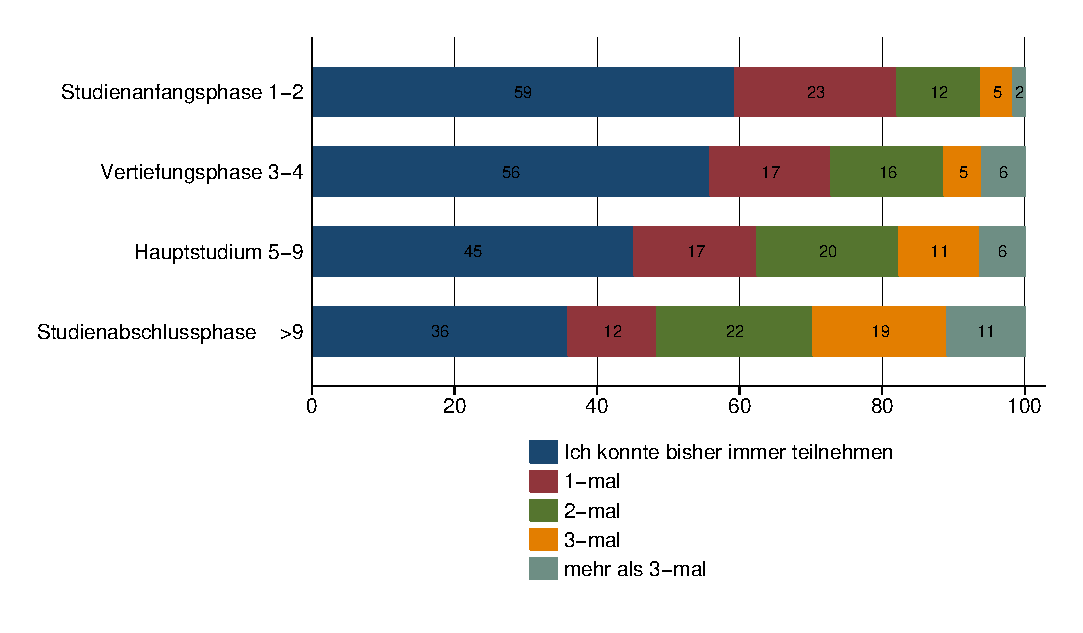
\includegraphics[
%  defaultresolution=72 !,
%  bmpsizefast=false
%]{image}
%\end{verbatim}
% \end{quote}
%
% \subsubsection{Hints}
%
% \begin{itemize}
% \item My version of \xfile{dvips.def} 1999/02/16 v3.0i defines
%       rules for the supported bitmap extensions, but does not
%       include them in the list of extensions that are tried
%       if the file name is not given with an extension.
%       In such a case, the list of extensions can be set
%       by \cs{DeclareGraphicsExtensions}, see \xpackage{grfguide}.
%       The following code just extends the list:
%       \begin{quote}
%\begin{verbatim}
%\makeatletter
%\g@addto@macro\Gin@extensions{,.bmp,.pcx,.msp}
%\makeatother
%\end{verbatim}
%       \end{quote}
% \item My version of \xfile{dvipdfm.def} 1998/11/24 vx.x misses
%       the graphics rule for PNG files. It can be added by:
%       \begin{quote}
%\begin{verbatim}
%\DeclareGraphicsRule{.png}{bmp}{.bb}{#1}
%\end{verbatim}
%       \end{quote}
%       See the previous issue to add the extension \xfile{.png} to the list
%       of extensions for package \xpackage{graphics}.
% \end{itemize}
%
% \subsubsection{Test program}
%
% There is a test program \xfile{bmpsize-test.tex}. Run it through
% \verb|latex|, \verb|pdflatex|, or \verb|pdftex|. Then given
% image files are inspected and the result is printed.
%
% \subsubsection{Interface for programmers}
%
% The macro names of the parsers are \verb|\bmpsize@read@|\meta{type}.
% Example: \cs{bmpsize@read@jpg} in case of JPEG.
%
% A parser sets the switch \cs{ifbmpsize@ok} to true, if it
% could successfully parse the image file.
% The width and height are returnd in \cs{bmpsize@width} and
% \cs{bmpsize@height}. If information about density is available,
% it is used to calculate width and height of the image, otherwise
% the values given by option \xoption{defaultresolution} is used.
% \xoption{resolution} overwrites the values in the image file.
%
% \subsection{Improved bitmap inclusion}
%
% Some drivers for package \xpackage{graphics} define the graphics
% type \xoption{bmp} for bitmap images. The code in the standard
% drivers for \xoption{dvips}, \xoption{dvipdfm}, and \xoption{dvipdfmx}
% is very basic and misses essential features of the
% package \xpackage{graphicx}. Therefore the code for bitmap
% inclusion is automatically rewritten by this package to add
% the following features:
% \begin{itemize}
% \item Support for \xoption{viewport} and \xoption{trim}.
% \item Support for \xoption{clip}.
% \item In case of \xoption{dvipdfm} and \xoption{dvipdfmx} the
%       bitmap images are reused and not included again if they
%       are used more than once.
% \end{itemize}
% However, there is a difference between \xoption{dvipdfm} and
% \xoption{dvipdfmx}, especially if images are reused. In the
% former case the reused box has width and height of 1bp, in the
% latter case its natural width. Thus the correct driver option must be given.
% \xoption{dvipdfm} and \xoption{dvipdfmx} are not equivalent.
%
% Older versions of \xoption{dvipdfmx} uses a size of 1in. However I do
% want to distinguish between versions of the same program. Therefore the
% support of these older versions has stopped with version 1.6 of this package.
% Use version dvipdfmx-20090708 or newer (some few versions before will
% probably also work, but I don't want to investigate this further).
%
% \StopEventually{
% }
%
% \section{Implementation}
%
% \subsection{Basic package \xpackage{bmpsize-base}}
%
%    Identification.
%    \begin{macrocode}
%<*base>
\ProvidesPackage{bmpsize-base}%
  [2009/09/04 v1.6 Basic part of bmpsize (HO)]%
%    \end{macrocode}
%    Modules of package \xpackage{fp} are used for calculations.
%    \begin{macrocode}
\RequirePackage{fp-basic}
\RequirePackage{fp-snap}
%    \end{macrocode}
%    Package \xpackage{fp} uses nested \cs{loop} structures.
%    That breaks with the plain-\TeX\ version of \cs{loop}.
%    Therefore we use the \LaTeX\ variant.
%    \begin{macro}{\@bmpsize@plain@loop}
%    \begin{macrocode}
\long\def\@bmpsize@plain@loop#1\repeat{%
  \def\iterate{%
    #1\relax
    \expandafter\iterate\fi
  }%
  \iterate
  \let\iterate\relax
}
%    \end{macrocode}
%    \end{macro}
%    \begin{macrocode}
\RequirePackage{pdftexcmds}[2007/11/11]
%    \end{macrocode}
%    \begin{macrocode}
\newif\ifbmpsize@ok
\let\@bmpsize@ok\bmpsize@oktrue

\newif\if@bmpsize@bigendian
\newif\if@bmpsize@absnum
\newif\if@bmpsize@user@resolution
\newif\if@bmpsize@fast
\@bmpsize@fasttrue

\def\@bmpsize@init{%
  \let\@bmpsize@org@plain@loop\loop
  \let\loop\@bmpsize@plain@loop
  \bmpsize@okfalse
  \@bmpsize@bigendiantrue
  \@bmpsize@absnumfalse
  \let\bmpsize@pixelwidth\relax
  \let\bmpsize@pixelheight\relax
  \let\bmpsize@pixelx\relax
  \let\bmpsize@pixely\relax
  \let\bmpsize@unit\relax
  \let\bmpsize@pixelxdenom\relax
  \let\bmpsize@pixelydenom\relax
  \let\bmpsize@orientation\relax
}

\def\@bmpsize@stop#1\@nil{}

\def\@bmpsize@loop#1{%
  #1%
  \@bmpsize@loop{#1}%
}
\def\@bmpsize@break#1\@bmpsize@loop#2{}

\def\@bmpsize@size#1#2#3{%
  \edef#3{\pdf@filesize{#1}}%
  \ifx#3\@empty
    \expandafter\@bmpsize@stop
  \fi
  \ifnum#3<#2\relax
    \expandafter\@bmpsize@stop
  \fi
}

\def\@bmpsize@read#1#2#3{%
  \edef\@bmpsize@buf{\pdf@filedump{#3}{#2}{#1}}%
  \edef\@bmpsize@temp{%
    \noexpand\@bmpsize@check@byte{#2}\@bmpsize@buf{}{}\noexpand\\%
  }%
  \@bmpsize@temp
}
\def\@bmpsize@fillbuf#1{%
  \ifx\@bmpsize@buf\@empty
    \expandafter\@firstofone
  \else
    \expandafter\@gobble
  \fi
  {%
    \edef\@bmpsize@buf{%
      \pdf@filedump{\bmpsize@offset}{\bmpsize@fillbuflength}{#1}%
    }%
    \ifx\@bmpsize@buf\@empty
      \expandafter\@bmpsize@stop
    \fi
    \edef\bmpsize@offset{\the\numexpr\bmpsize@offset+\bmpsize@fillbuflength}%
  }%
}
\def\bmpsize@fillbuflength{10}

\def\@bmpsize@append#1#2#3{%
  \edef#1{#2#3}%
}
\def\@bmpsize@pushback#1{%
  \edef\@bmpsize@buf{#1\@bmpsize@buf}%
}

\def\@bmpsize@iswhite#1{%
  \ifnum\pdf@strcmp{#1}{09}=\z@
  \else
    \ifnum\pdf@strcmp{#1}{0A}=\z@
    \else
      \ifnum\pdf@strcmp{#1}{0D}=\z@
      \else
        \ifnum\pdf@strcmp{#1}{20}=\z@
        \else
          1%
        \fi
      \fi
    \fi
  \fi
  \space
}
\def\@bmpsize@isdigit#1{%
  \ifnum\pdf@strcmp{#1}{30}<\z@
    1%
  \else
    \ifnum\pdf@strcmp{#1}{39}>\z@
      1%
    \fi
  \fi
  \space
}

\def\@bmpsize@check@byte#1#2#3{%
  \ifnum#1<\@ne
    \csname fi\endcsname
    \@bmpsize@cleanup@end
  \else
    \csname fi\endcsname
  \ifx!#2#3!%
    \csname fi\endcsname
    \@bmpsize@stop
  \else
    \csname fi\endcsname
    \expandafter\@bmpsize@check@byte\expandafter{\the\numexpr#1-1}%
}
\def\@bmpsize@cleanup@end#1\\{}

\def\@bmpsize@swap@maybe#1{%
  \if@bmpsize@bigendian
  \else
    \edef#1{\expandafter\@bmpsize@@swap#1\@empty\@empty\@empty\@empty}%
  \fi
}
\def\@bmpsize@@swap#1#2#3#4#5#6#7#8{%
  #7#8#5#6#3#4#1#2%
}

\def\@bmpsize@skip@one{%
  \edef\@bmpsize@buf{\expandafter\@gobbletwo\@bmpsize@buf}%
}
\def\@bmpsize@skip@two{%
  \edef\@bmpsize@buf{\expandafter\@gobblefour\@bmpsize@buf}%
}
\def\@bmpsize@skip@four{%
  \edef\@bmpsize@buf{%
    \expandafter\expandafter\expandafter\@gobblefour\expandafter
    \@gobblefour\@bmpsize@buf
  }%
}

\def\@bmpsize@grab#1#2{%
  \edef#1{\noexpand\@bmpsize@grab@byte#2=\@bmpsize@buf\noexpand\\}%
  \edef#1{#1}%
}
\def\@bmpsize@grab@byte#1=#2#3{%
  #2#3%
  \ifnum#1>\@ne
    \expandafter\@bmpsize@grab@byte\the\numexpr#1-1\expandafter=%
  \else
    \expandafter\@bmpsize@cleanup@end
  \fi
}

\def\@bmpsize@abs@maybe#1{%
  \let\@bmpsize@temp\relax
  \if@bmpsize@absnum
    \ifnum"\expandafter\@car#1\@nil>7 %
      \edef#1{\expandafter\@bmpsize@abs@byte#1\relax}%
      \ifnum\pdf@strcmp{#1}{7FFFFFFF}=\z@
        \let\@bmpsize@temp\@bmpsize@stop
      \else
        \def\@bmpsize@temp{\edef#1{\the\numexpr#1+1}}%
      \fi
    \fi
  \fi
}
\def\@bmpsize@abs@byte#1{%
  \ifx#1\relax
  \else
    \ifcase"0#1 %
      F\or E\or D\or C\or B\or A\or 9\or 8\or
      7\or 6\or 5\or 4\or 3\or 2\or 1\or 0%
    \fi
    \expandafter\@bmpsize@abs@byte
  \fi
}

\def\@bmpsize@num@one#1{%
  \@bmpsize@grab#11%
  \@bmpsize@abs@maybe#1%
  \edef#1{\number"#1}%
  \@bmpsize@temp
  \@bmpsize@skip@one
}
\def\@bmpsize@num@two#1{%
  \@bmpsize@grab#12%
  \@bmpsize@swap@maybe#1%
  \@bmpsize@abs@maybe#1%
  \edef#1{\number"#1}%
  \@bmpsize@temp
  \@bmpsize@skip@two
}
\def\@bmpsize@num@four#1{%
  \@bmpsize@grab#14%
  \@bmpsize@swap@maybe#1%
  \@bmpsize@abs@maybe#1%
  \ifnum\pdf@strcmp{#1}{7FFFFFFF}>\z@
    \expandafter\@bmpsize@stop
  \fi
  \edef#1{\number"#1}%
  \@bmpsize@temp
  \@bmpsize@skip@four
}

\def\@bmpsize@div#1#2#3{% #1 := #2/#3
  \FPdiv#1{#2}{#3}%
  \@bmpsize@beautify#1%
}
\def\@bmpsize@beautify#1{%
  \FPifint#1%
    \edef#1{\expandafter\@bmpsize@trunc#1.\@nil}%
  \else
    \edef#1{\expandafter\@bmpsize@cleanup@frac#1.\@nil}%
  \fi
}
\def\@bmpsize@trunc#1.#2\@nil{#1}
% #1 isn't an integer, thus we should have at least one
% necessary digit after the dot
\def\@bmpsize@cleanup@frac#1.#2#3.#4\@nil{%
  #1.#2%
  \ifx\\#3\\%
  \else
    \@bmpsize@cleanup@fracdigits#3000000000\@nil
  \fi
}
\def\@bmpsize@cleanup@fracdigits#1#2#3#4#5#6#7#8#9{%
  \ifcase#9 %
    \ifcase#8 %
      \ifcase#7 %
        \ifcase#6 %
          \ifcase#5 %
            \ifcase #4 %
              \ifcase #3 %
                \ifcase #2 %
                  \ifcase #1 %
                  \else
                    #1%
                  \fi
                \else
                  #1#2%
                \fi
              \else
                #1#2#3%
              \fi
            \else
              #1#2#3#4%
            \fi
          \else
            #1#2#3#4#5%
          \fi
        \else
          #1#2#3#4#5#6%
        \fi
      \else
        #1#2#3#4#5#6#7%
      \fi
    \else
      #1#2#3#4#5#6#7#8%
    \fi
  \else
    #1#2#3#4#5#6#7#8#9%
  \fi
  \@bmpsize@trunc.%
}

\def\@bmpsize@end{%
  \ifbmpsize@ok
    \ifx\bmpsize@pixelwidth\relax
      \bmpsize@okfalse
    \fi
    \ifx\bmpsize@pixelheight\relax
      \bmpsize@okfalse
    \fi
  \fi
  \ifbmpsize@ok
    \ifnum\bmpsize@pixelwidth>\z@
    \else
      \bmpsize@okfalse
    \fi
    \ifnum\bmpsize@pixelheight>\z@
    \else
      \bmpsize@okfalse
    \fi
  \fi
  \ifbmpsize@ok
    \ifcase 0%
      \ifx\bmpsize@pixelx\relax 1 \fi
      \ifx\bmpsize@pixely\relax 1 \fi
      \ifnum\bmpsize@pixelx>\z@\else 1 \fi
      \ifnum\bmpsize@pixely>\z@\else 1 \fi
      \ifx\bmpsize@pixelxdenom\relax
         \ifx\bmpsize@pixelydenom\relax\else 1 \fi
      \else
        \ifnum\bmpsize@pixelxdenom>\z@\else 1 \fi
      \fi
      \ifx\bmpsize@pixelydenom\relax
      \else
        \ifnum\bmpsize@pixelydenom>\z@\else 1 \fi
      \fi
    \else
      \let\bmpsize@pixelx\relax
      \let\bmpsize@pixely\relax
      \let\bmpsize@unit\relax
      \let\bmpsize@pixelxdenom\relax
      \let\bmpsize@pixelydenom\relax
    \fi
    \ifx\bmpsize@pixelxdenom\relax
    \else
      \@bmpsize@div\bmpsize@pixelx\bmpsize@pixelx\bmpsize@pixelxdenom
      \@bmpsize@div\bmpsize@pixely\bmpsize@pixely\bmpsize@pixelydenom
      \let\bmpsize@pixelxdenom\relax
      \let\bmpsize@pixelydenom\relax
    \fi
    \ifcase 0\ifx\bmpsize@unit\relax 1\fi
             \if@bmpsize@user@resolution 1\fi
             \relax
      \let\bmpsize@calc@unit\bmpsize@unit
      \let\bmpsize@calc@pixelx\bmpsize@pixelx
      \let\bmpsize@calc@pixely\bmpsize@pixely
    \else
      \let\bmpsize@calc@unit\bmpsize@unit@default
      \let\bmpsize@calc@pixelx\bmpsize@pixelx@default
      \let\bmpsize@calc@pixely\bmpsize@pixely@default
      \ifx\bmpsize@calc@pixely\Gin@exclamation
        \ifx\bmpsize@pixelx\relax
          \let\bmpsize@calc@pixely\bmpsize@calc@pixelx
        \else
          \FPdiv\bmpsize@calc@pixely\bmpsize@calc@pixelx\bmpsize@pixelx
          \FPmul\bmpsize@calc@pixely\bmpsize@calc@pixely\bmpsize@pixely
        \fi
      \else
        \ifx\bmpsize@calc@pixelx\Gin@exclamation
          \ifx\bmpsize@pixelx\relax
            \let\bmpsize@calc@pixelx\bmpsize@calc@pixely
          \else
            \FPdiv\bmpsize@calc@pixelx\bmpsize@calc@pixely\bmpsize@pixely
            \FPmul\bmpsize@calc@pixelx\bmpsize@calc@pixelx\bmpsize@pixelx
          \fi
        \fi
      \fi
    \fi
    \FPdiv\bmpsize@width\bmpsize@pixelwidth\bmpsize@calc@pixelx
    \FPdiv\bmpsize@height\bmpsize@pixelheight\bmpsize@calc@pixely
    % calculation of width and height in bp for package graphics
    % 1in = 72bp = 72.27pt, 72/72.27 = 8/8.03, 1pt = 65536sp
    \if@bmpsize@fast
      \edef\bmpsize@width{%
        \strip@pt\dimexpr.99626\dimexpr
        \bmpsize@width\dimexpr\bmpsize@calc@unit
      }%
      \edef\bmpsize@height{%
        \strip@pt\dimexpr.99626\dimexpr
        \bmpsize@height\dimexpr\bmpsize@calc@unit
      }%
    \else
      \edef\@bmpsize@temp{\number\dimexpr\bmpsize@calc@unit}%
      \ifnum\@bmpsize@temp>100000 %
        \FPmul\@bmpsize@temp\@bmpsize@temp{0.00001}%
        \def\@bmpsize@corr{100000}%
      \else
        \let\@bmpsize@corr\relax
      \fi
      \FPmul\bmpsize@width\bmpsize@width\@bmpsize@temp
      \FPmul\bmpsize@height\bmpsize@height\@bmpsize@temp
      \FPmul\bmpsize@width\bmpsize@width{8}%
      \FPmul\bmpsize@height\bmpsize@height{8}%
      \FPdiv\bmpsize@width\bmpsize@width{8.03}%
      \FPdiv\bmpsize@height\bmpsize@height{8.03}%
      \FPdiv\bmpsize@width\bmpsize@width{65536}%
      \FPdiv\bmpsize@height\bmpsize@height{65536}%
      \ifx\@bmpsize@corr\relax
      \else
        \FPmul\bmpsize@width\bmpsize@width\@bmpsize@corr
        \FPmul\bmpsize@height\bmpsize@height\@bmpsize@corr
      \fi
      \FPround\bmpsize@width\bmpsize@width{5}%
      \FPround\bmpsize@height\bmpsize@height{5}%
      \@bmpsize@beautify\bmpsize@width
      \@bmpsize@beautify\bmpsize@height
    \fi
  \fi
  \let\loop\@bmpsize@org@plain@loop
}
\def\bmpsize@unit@default{72.27pt}% more accurate than 1in
\def\bmpsize@pixelx@default{72}
\let\bmpsize@pixely@default\Gin@exclamation

\def\bmpsize@types{png,jpg,bmp,gif,tiff,pnm,pam,xpm,tga,pcx,msp,sgi}
%</base>
%    \end{macrocode}
%
% \subsection{Bitmap formats}
%
% \subsubsection{png}
%
%\iffalse
%<*ignore>
%\fi
%\begin{verbatim}
%begin png
%big-endian
%
%read 24 0
%grab 8        -> $temp
%check streq $temp [0x89 "PNG" 0x0D 0x0A 0x1A 0x0A]
%num 4         -> $length
%grab 4        -> $temp
%check streq $temp ["IHDR"]
%num 4         -> $pixelwidth
%num 4         -> $pixelheight
%ok
%assign numexpr(20 + $length) -> $offset
%loop
%  read 8 $offset
%  num 4       -> $length
%  grab 4      -> $temp
%  if streq $temp ["IDAT"]
%    stop
%  fi
%  if streq $temp ["pHYs"]
%    read 9 numexpr($offset + 8)
%    num 4     -> $pixelx
%    num 4     -> $pixely
%    grab 1     -> $temp
%    if numeq $temp 1
%      assign {100cm} -> $unit
%    fi
%    stop
%  fi
%  assign numexpr($offset + 12 + $length) -> $offset
%repeat
%end
%\end{verbatim}
%\iffalse
%</ignore>
%\fi
%    \begin{macro}{\bmpsize@read@png}
%    \begin{macrocode}
%<*base>
\def\bmpsize@read@png#1{%
  \@bmpsize@init
  \@bmpsize@bigendiantrue
  \@bmpsize@read{#1}{24}{0}%
  \@bmpsize@grab\bmpsize@temp{8}%
  \@bmpsize@skip@four
  \@bmpsize@skip@four
  \ifnum\pdf@strcmp{\bmpsize@temp}{89504E470D0A1A0A}=\z@
  \else
    \expandafter\@bmpsize@stop
  \fi
  \@bmpsize@num@four\bmpsize@length
  \@bmpsize@grab\bmpsize@temp{4}%
  \@bmpsize@skip@four
  \ifnum\pdf@strcmp{\bmpsize@temp}{49484452}=\z@
  \else
    \expandafter\@bmpsize@stop
  \fi
  \@bmpsize@num@four\bmpsize@pixelwidth
  \@bmpsize@num@four\bmpsize@pixelheight
  \@bmpsize@ok
  \edef\bmpsize@offset{\the\numexpr20+\bmpsize@length}%
  \@bmpsize@loop{%
    \@bmpsize@read{#1}{8}{\bmpsize@offset}%
    \@bmpsize@num@four\bmpsize@length
    \@bmpsize@grab\bmpsize@temp{4}%
    \@bmpsize@skip@four
    \ifnum\pdf@strcmp{\bmpsize@temp}{49444154}=\z@
      \expandafter\@firstofone
    \else
      \expandafter\@gobble
    \fi
    {%
      \@bmpsize@stop
    }%
    \ifnum\pdf@strcmp{\bmpsize@temp}{70485973}=\z@
      \expandafter\@firstofone
    \else
      \expandafter\@gobble
    \fi
    {%
      \@bmpsize@read{#1}{9}{\numexpr\bmpsize@offset+8\relax}%
      \@bmpsize@num@four\bmpsize@pixelx
      \@bmpsize@num@four\bmpsize@pixely
      \@bmpsize@grab\bmpsize@temp{1}%
      \@bmpsize@skip@one
      \ifnum\bmpsize@temp=1\relax
        \expandafter\@firstofone
      \else
        \expandafter\@gobble
      \fi
      {%
        \def\bmpsize@unit{100cm}%
      }%
      \@bmpsize@stop
    }%
    \edef\bmpsize@offset{\the\numexpr\bmpsize@offset+12+\bmpsize@length}%
  }%
  \@bmpsize@stop
  \@nil
  \@bmpsize@end
}%
%</base>
%    \end{macrocode}
%    \end{macro}
%
% \subsubsection{jpg}
%
%\iffalse
%<*ignore>
%\fi
%\begin{verbatim}
%begin jpg
%
%read 3 0
%grab 3      -> $temp % SOI and 0xFF
%check streq $temp [0xFF 0xD8 0xFF]
%assign {2} -> $offset
%assign {0} -> $exifdensity
%loop
%  read 4 $offset
%  grab 1    -> $temp
%  check streq $temp [0xFF]
%  num 1    -> $temp
%  if numeq $temp 0xDA % SOS
%    stop
%  fi
%  % look for JFIF APP0 segment
%  if numeq $temp 0xE0 % APP0
%    num 2       -> $length
%    if numeq $exifdensity 0
%      if numge $length 16 % a JFIF segment has 16 bytes at least
%        read 12 numexpr($offset + 4)
%        grab 5      -> $temp % identifier
%        if streq $temp ["JFIF" 0x0]
%          check numge $length 16
%          skip 2 % version
%          num 1       -> $temp % units
%          if numeq $temp 1
%            assign {72.27pt} -> $unit
%          else
%            if numeq $temp 2
%              assign {1cm} -> $unit
%            fi
%          fi
%          num 2    -> $pixelx
%          num 2    -> $pixely
%        fi
%      fi
%    fi
%  else
%    if numeq $temp 0xE1 % APP1
%      % look for Exif APP1 segment
%      num 2 -> $length
%      if numge $length 20 % identifier (6) + Tiff header (8) + first IFD (>=6)
%        read 20 numexpr($offset + 4)
%        grab 6 -> $temp
%        if streq $temp ["Exif" 0x0 0x0]
%          assign numexpr($offset + 10) -> $exifoffset
%          % read TIFF header
%          grab 2 -> $temp
%          if streq $temp ["II"]
%            little-endian
%          else
%            check streq $temp ["MM"]
%            % big-endian
%          fi
%          num 2 -> $temp
%          check numeq $temp 42
%          num 4 -> $temp % offset of first IFD
%          check numgt $temp 0
%          % read first IFD
%          assign numexpr($temp + $exifoffset) -> $off
%          read 2 $off
%          num 2 -> $entries
%          assign numexpr($off + 2) -> $off
%          loop
%            if numeq $entries 0
%              break
%            fi
%            assign numexpr($entries - 1) -> $entries
%            % entry format:
%            % 2 tag
%            % 2 field type
%            % 4 count
%            % 4 value/offset
%            read 12 $off
%            assign numexpr($off + 12) -> $off
%            num 2 -> $tag
%            if numeq $tag 296 % ResolutionUnit
%              skip 6 % type: 3 (short), count: 1
%              num 2 -> $temp
%              ifcase $temp
%              or % 1
%                clear $unit
%              or % 2
%                assign {72.27pt} -> $unit
%              or % 3
%                assign {1cm} -> $unit
%              else
%                clear $unit % unknown
%              fi
%              ifcase $temp
%              or % 1
%              or % 2
%                assign {1} -> $exifdensity
%              or % 3
%                assign {1} -> $exifdensity
%              else
%                assign $exifdensity -> $exifdensity
%              fi
%            fi
%            % 256 ImageWidth (use width of JPG part)
%            % 257 ImageHeight (use height of JPG part)
%            if numeq $tag 274 % Orientation
%              skip 6 % type: 3 (short), count: 1
%              num 2 -> $temp
%              if numge $temp 0 
%                if numle $temp 8
%                  assign $temp -> $orientation
%                fi
%              fi
%            fi
%            if numeq $tag 282 % XResolution
%              skip 6
%              num 4 -> $temp
%              read 8 numexpr($temp + $exifoffset)
%              num 4 -> $pixelx
%              num 4 -> $temp
%              if numeq $temp 1
%              else
%                assign numexpr($temp) -> $pixelxdenom
%                % div $pixelx $temp -> $pixelx
%              fi
%            fi
%            if numeq $tag 283 % YResolution
%              skip 6
%              num 4 -> $temp
%              read 8 numexpr($temp + $exifoffset)
%              num 4 -> $pixely
%              num 4 -> $temp
%              if numeq $temp 1
%              else
%                assign numexpr($temp) -> $pixelydenom
%                % div $pixely $temp -> $pixely
%              fi
%            fi
%          repeat
%          big-endian
%        fi
%      fi
%    else
%      assign numexpr($temp - 0xC0) -> $temp
%      ifcase $temp % SOF_0
%      or % SOF_1
%      or % SOF_2
%      or % SOF_3
%      or % DHT
%        assign {-1} -> $temp
%      or % SOF_5
%      or % SOF_6
%      or % SOF_7
%      or % JPG
%        assign {-1} -> $temp
%      or % SOF_9
%      or % SOF_10
%      or % SOF_11
%      or % DAC
%        assign {-1} -> $temp
%      or % SOF_13
%      or % SOF_14
%      or % SOF_15
%      else
%        assign {-1} -> $temp
%      fi
%      if numeq $temp -1
%      else
%        read 4 numexpr($offset + 5)
%        num 2  -> $pixelheight
%        num 2  -> $pixelwidth
%        if numeq $pixelheight 0
%          clear $pixelheight
%          stop
%        fi
%        ok
%        stop
%      fi
%      num 2 -> $length
%    fi
%  fi
%  assign numexpr($offset + $length + 2) -> $offset
%repeat
%end
%\end{verbatim}
%\iffalse
%</ignore>
%\fi
%    \begin{macro}{\bmpsize@read@jpg}
%    \begin{macrocode}
%<*base>
\def\bmpsize@read@jpg#1{%
  \@bmpsize@init
  \@bmpsize@read{#1}{3}{0}%
  \@bmpsize@grab\bmpsize@temp{3}%
  \@bmpsize@skip@two
  \@bmpsize@skip@one
  \ifnum\pdf@strcmp{\bmpsize@temp}{FFD8FF}=\z@
  \else
    \expandafter\@bmpsize@stop
  \fi
  \def\bmpsize@offset{2}%
  \def\bmpsize@exifdensity{0}%
  \@bmpsize@loop{%
    \@bmpsize@read{#1}{4}{\bmpsize@offset}%
    \@bmpsize@grab\bmpsize@temp{1}%
    \@bmpsize@skip@one
    \ifnum\pdf@strcmp{\bmpsize@temp}{FF}=\z@
    \else
      \expandafter\@bmpsize@stop
    \fi
    \@bmpsize@num@one\bmpsize@temp
    \ifnum\bmpsize@temp=218\relax
      \expandafter\@firstofone
    \else
      \expandafter\@gobble
    \fi
    {%
      \@bmpsize@stop
    }%
    \ifnum\bmpsize@temp=224\relax
      \expandafter\@firstoftwo
    \else
      \expandafter\@secondoftwo
    \fi
    {%
      \@bmpsize@num@two\bmpsize@length
      \ifnum\bmpsize@exifdensity=0\relax
        \expandafter\@firstofone
      \else
        \expandafter\@gobble
      \fi
      {%
        \unless\ifnum\bmpsize@length<16\relax
          \expandafter\@firstofone
        \else
          \expandafter\@gobble
        \fi
        {%
          \@bmpsize@read{#1}{12}{\numexpr\bmpsize@offset+4\relax}%
          \@bmpsize@grab\bmpsize@temp{5}%
          \@bmpsize@skip@four
          \@bmpsize@skip@one
          \ifnum\pdf@strcmp{\bmpsize@temp}{4A46494600}=\z@
            \expandafter\@firstofone
          \else
            \expandafter\@gobble
          \fi
          {%
            \ifnum\bmpsize@length<16\relax
              \expandafter\@bmpsize@stop
            \fi
            \@bmpsize@skip@two
            \@bmpsize@num@one\bmpsize@temp
            \ifnum\bmpsize@temp=1\relax
              \expandafter\@firstoftwo
            \else
              \expandafter\@secondoftwo
            \fi
            {%
              \def\bmpsize@unit{72.27pt}%
            }{%
              \ifnum\bmpsize@temp=2\relax
                \expandafter\@firstofone
              \else
                \expandafter\@gobble
              \fi
              {%
                \def\bmpsize@unit{1cm}%
              }%
            }%
            \@bmpsize@num@two\bmpsize@pixelx
            \@bmpsize@num@two\bmpsize@pixely
          }%
        }%
      }%
    }{%
      \ifnum\bmpsize@temp=225\relax
        \expandafter\@firstoftwo
      \else
        \expandafter\@secondoftwo
      \fi
      {%
        \@bmpsize@num@two\bmpsize@length
        \unless\ifnum\bmpsize@length<20\relax
          \expandafter\@firstofone
        \else
          \expandafter\@gobble
        \fi
        {%
          \@bmpsize@read{#1}{20}{\numexpr\bmpsize@offset+4\relax}%
          \@bmpsize@grab\bmpsize@temp{6}%
          \@bmpsize@skip@four
          \@bmpsize@skip@two
          \ifnum\pdf@strcmp{\bmpsize@temp}{457869660000}=\z@
            \expandafter\@firstofone
          \else
            \expandafter\@gobble
          \fi
          {%
            \edef\bmpsize@exifoffset{\the\numexpr\bmpsize@offset+10}%
            \@bmpsize@grab\bmpsize@temp{2}%
            \@bmpsize@skip@two
            \ifnum\pdf@strcmp{\bmpsize@temp}{4949}=\z@
              \expandafter\@firstoftwo
            \else
              \expandafter\@secondoftwo
            \fi
            {%
              \@bmpsize@bigendianfalse
            }{%
              \ifnum\pdf@strcmp{\bmpsize@temp}{4D4D}=\z@
              \else
                \expandafter\@bmpsize@stop
              \fi
            }%
            \@bmpsize@num@two\bmpsize@temp
            \ifnum\bmpsize@temp=42\relax
            \else
              \expandafter\@bmpsize@stop
            \fi
            \@bmpsize@num@four\bmpsize@temp
            \ifnum\bmpsize@temp>0\relax
            \else
              \expandafter\@bmpsize@stop
            \fi
            \edef\bmpsize@off{\the\numexpr\bmpsize@temp+\bmpsize@exifoffset}%
            \@bmpsize@read{#1}{2}{\bmpsize@off}%
            \@bmpsize@num@two\bmpsize@entries
            \edef\bmpsize@off{\the\numexpr\bmpsize@off+2}%
            \@bmpsize@loop{%
              \ifnum\bmpsize@entries=0\relax
                \expandafter\@firstofone
              \else
                \expandafter\@gobble
              \fi
              {%
                \@bmpsize@break
              }%
              \edef\bmpsize@entries{\the\numexpr\bmpsize@entries-1}%
              \@bmpsize@read{#1}{12}{\bmpsize@off}%
              \edef\bmpsize@off{\the\numexpr\bmpsize@off+12}%
              \@bmpsize@num@two\bmpsize@tag
              \ifnum\bmpsize@tag=296\relax
                \expandafter\@firstofone
              \else
                \expandafter\@gobble
              \fi
              {%
                \@bmpsize@skip@four
                \@bmpsize@skip@two
                \@bmpsize@num@two\bmpsize@temp
                \ifcase\bmpsize@temp\relax
                \or
                  \let\bmpsize@unit\relax
                \or
                  \def\bmpsize@unit{72.27pt}%
                \or
                  \def\bmpsize@unit{1cm}%
                \else
                  \let\bmpsize@unit\relax
                \fi
                \ifcase\bmpsize@temp\relax
                \or
                \or
                  \def\bmpsize@exifdensity{1}%
                \or
                  \def\bmpsize@exifdensity{1}%
                \else
                  \let\bmpsize@exifdensity\bmpsize@exifdensity
                \fi
              }%
              \ifnum\bmpsize@tag=274\relax
                \expandafter\@firstofone
              \else
                \expandafter\@gobble
              \fi
              {%
                \@bmpsize@skip@four
                \@bmpsize@skip@two
                \@bmpsize@num@two\bmpsize@temp
                \unless\ifnum\bmpsize@temp<0\relax
                  \expandafter\@firstofone
                \else
                  \expandafter\@gobble
                \fi
                {%
                  \unless\ifnum\bmpsize@temp>8\relax
                    \expandafter\@firstofone
                  \else
                    \expandafter\@gobble
                  \fi
                  {%
                    \let\bmpsize@orientation\bmpsize@temp
                  }%
                }%
              }%
              \ifnum\bmpsize@tag=282\relax
                \expandafter\@firstofone
              \else
                \expandafter\@gobble
              \fi
              {%
                \@bmpsize@skip@four
                \@bmpsize@skip@two
                \@bmpsize@num@four\bmpsize@temp
                \@bmpsize@read{#1}{8}{\numexpr\bmpsize@temp+\bmpsize@exifoffset\relax}%
                \@bmpsize@num@four\bmpsize@pixelx
                \@bmpsize@num@four\bmpsize@temp
                \ifnum\bmpsize@temp=1\relax
                  \expandafter\@gobble
                \else
                  \expandafter\@firstofone
                \fi
                {%
                  \edef\bmpsize@pixelxdenom{\the\numexpr\bmpsize@temp}%
                }%
              }%
              \ifnum\bmpsize@tag=283\relax
                \expandafter\@firstofone
              \else
                \expandafter\@gobble
              \fi
              {%
                \@bmpsize@skip@four
                \@bmpsize@skip@two
                \@bmpsize@num@four\bmpsize@temp
                \@bmpsize@read{#1}{8}{\numexpr\bmpsize@temp+\bmpsize@exifoffset\relax}%
                \@bmpsize@num@four\bmpsize@pixely
                \@bmpsize@num@four\bmpsize@temp
                \ifnum\bmpsize@temp=1\relax
                  \expandafter\@gobble
                \else
                  \expandafter\@firstofone
                \fi
                {%
                  \edef\bmpsize@pixelydenom{\the\numexpr\bmpsize@temp}%
                }%
              }%
            }%
            \@bmpsize@bigendiantrue
          }%
        }%
      }{%
        \edef\bmpsize@temp{\the\numexpr\bmpsize@temp-192}%
        \ifcase\bmpsize@temp\relax
        \or
        \or
        \or
        \or
          \def\bmpsize@temp{-1}%
        \or
        \or
        \or
        \or
          \def\bmpsize@temp{-1}%
        \or
        \or
        \or
        \or
          \def\bmpsize@temp{-1}%
        \or
        \or
        \or
        \else
          \def\bmpsize@temp{-1}%
        \fi
        \ifnum\bmpsize@temp=-1\relax
          \expandafter\@gobble
        \else
          \expandafter\@firstofone
        \fi
        {%
          \@bmpsize@read{#1}{4}{\numexpr\bmpsize@offset+5\relax}%
          \@bmpsize@num@two\bmpsize@pixelheight
          \@bmpsize@num@two\bmpsize@pixelwidth
          \ifnum\bmpsize@pixelheight=0\relax
            \expandafter\@firstofone
          \else
            \expandafter\@gobble
          \fi
          {%
            \let\bmpsize@pixelheight\relax
            \@bmpsize@stop
          }%
          \@bmpsize@ok
          \@bmpsize@stop
        }%
        \@bmpsize@num@two\bmpsize@length
      }%
    }%
    \edef\bmpsize@offset{\the\numexpr\bmpsize@offset+\bmpsize@length+2}%
  }%
  \@bmpsize@stop
  \@nil
  \@bmpsize@end
}%
%</base>
%    \end{macrocode}
%    \end{macro}
%
% \subsubsection{bmp}
%
%\iffalse
%<*ignore>
%\fi
%\begin{verbatim}
%begin bmp
%little-endian
%
%read 26 0
%grab 2 -> $temp
%check streq $temp ["BM"]
%skip 12
%% header size is 4 bytes in V3+, unknown for V1, V2,
%% known header sizes fit in 2 bytes
%num 2   -> $temp
%if numeq $temp 12 % V1
%  skip 2
%  num 2 -> $pixelwidth
%  num 2 -> $pixelheight
%  % no resolution entries
%  ok
%  stop
%fi
%if numeq $temp 64 % V2
%  skip 2
%  num 2 -> $pixelwidth
%  num 2 -> $pixelheight
%  % missing specification for resolution
%  ok
%  stop
%fi
%% V3, V4, V5
%skip 2
%num 4 -> $pixelwidth
%absnum 4 -> $pixelheight
%ok
%read 8 38
%num 4 -> $pixelx
%num 4 -> $pixely
%assign {100cm} -> $unit
%end
%\end{verbatim}
%\iffalse
%</ignore>
%\fi
%    \begin{macro}{\bmpsize@read@bmp}
%    \begin{macrocode}
%<*base>
\def\bmpsize@read@bmp#1{%
  \@bmpsize@init
  \@bmpsize@bigendianfalse
  \@bmpsize@read{#1}{26}{0}%
  \@bmpsize@grab\bmpsize@temp{2}%
  \@bmpsize@skip@two
  \ifnum\pdf@strcmp{\bmpsize@temp}{424D}=\z@
  \else
    \expandafter\@bmpsize@stop
  \fi
  \@bmpsize@skip@four
  \@bmpsize@skip@four
  \@bmpsize@skip@four
  \@bmpsize@num@two\bmpsize@temp
  \ifnum\bmpsize@temp=12\relax
    \expandafter\@firstofone
  \else
    \expandafter\@gobble
  \fi
  {%
    \@bmpsize@skip@two
    \@bmpsize@num@two\bmpsize@pixelwidth
    \@bmpsize@num@two\bmpsize@pixelheight
    \@bmpsize@ok
    \@bmpsize@stop
  }%
  \ifnum\bmpsize@temp=64\relax
    \expandafter\@firstofone
  \else
    \expandafter\@gobble
  \fi
  {%
    \@bmpsize@skip@two
    \@bmpsize@num@two\bmpsize@pixelwidth
    \@bmpsize@num@two\bmpsize@pixelheight
    \@bmpsize@ok
    \@bmpsize@stop
  }%
  \@bmpsize@skip@two
  \@bmpsize@num@four\bmpsize@pixelwidth
  \@bmpsize@absnumtrue
  \@bmpsize@num@four\bmpsize@pixelheight
  \@bmpsize@absnumfalse
  \@bmpsize@ok
  \@bmpsize@read{#1}{8}{38}%
  \@bmpsize@num@four\bmpsize@pixelx
  \@bmpsize@num@four\bmpsize@pixely
  \def\bmpsize@unit{100cm}%
  \@bmpsize@stop
  \@nil
  \@bmpsize@end
}%
%</base>
%    \end{macrocode}
%    \end{macro}
%
% \subsubsection{gif}
%
%\iffalse
%<*ignore>
%\fi
%\begin{verbatim}
%begin gif
%little-endian
%
%% Header
%read 13 0
%grab 3      -> $temp
%check streq $temp ["GIF"]
%skip 3      % version
%
%% Logical Screen Descriptor
%num 2       -> $pixelwidth
%num 2       -> $pixelheight
%skip 2
%num 1       -> $temp % Pixel Aspect Ratio
%if numeq $temp 0
%else
%  assign numexpr($temp + 15) -> $pixelx
%  assign {64}     -> $pixely
%fi
%ok
%end
%\end{verbatim}
%\iffalse
%</ignore>
%\fi
%    \begin{macro}{\bmpsize@read@gif}
%    \begin{macrocode}
%<*base>
\def\bmpsize@read@gif#1{%
  \@bmpsize@init
  \@bmpsize@bigendianfalse
  \@bmpsize@read{#1}{13}{0}%
  \@bmpsize@grab\bmpsize@temp{3}%
  \@bmpsize@skip@two
  \@bmpsize@skip@one
  \ifnum\pdf@strcmp{\bmpsize@temp}{474946}=\z@
  \else
    \expandafter\@bmpsize@stop
  \fi
  \@bmpsize@skip@two
  \@bmpsize@skip@one
  \@bmpsize@num@two\bmpsize@pixelwidth
  \@bmpsize@num@two\bmpsize@pixelheight
  \@bmpsize@skip@two
  \@bmpsize@num@one\bmpsize@temp
  \ifnum\bmpsize@temp=0\relax
    \expandafter\@gobble
  \else
    \expandafter\@firstofone
  \fi
  {%
    \edef\bmpsize@pixelx{\the\numexpr\bmpsize@temp+15}%
    \def\bmpsize@pixely{64}%
  }%
  \@bmpsize@ok
  \@bmpsize@stop
  \@nil
  \@bmpsize@end
}%
%</base>
%    \end{macrocode}
%    \end{macro}
%
% \subsubsection{tiff}
%
%\iffalse
%<*ignore>
%\fi
%\begin{verbatim}
%begin tiff
%% defaults
%assign {72.27pt} -> $unit
%
%% Image File Header
%read 8 0
%grab 2 -> $temp
%if streq $temp ["II"]
%  little-endian
%else
%  check streq $temp ["MM"]
%  big-endian
%fi
%num 2 -> $temp
%check numeq $temp 42
%num 4 -> $offset % first IFD (Image File Directory)
%
%% First IFD
%read 2 $offset
%assign numexpr($offset + 2) -> $offset
%num 2 -> $entries
%ok % must rely on checks at the end
%loop
%  if numeq $entries 0
%    stop
%  fi
%  assign numexpr($entries - 1) -> $entries
%  % entry format:
%  % 2 tag
%  % 2 field type
%  % 4 count
%  % 4 value/offset
%  read 12 $offset
%  assign numexpr($offset + 12) -> $offset
%  num 2 -> $tag % tag
%  if numeq $temp 296 % ResolutionUnit
%    skip 6 % type: 3 (short), count: 1
%    num 2 -> $temp
%    ifcase $temp
%    or % 1
%      clear $unit
%    or % 2
%      assign {72.27pt} -> $unit
%    or % 3
%      assign {1cm} -> $unit
%    else
%      clear $unit
%    fi
%  fi
%  if numeq $tag 256 % ImageWidth
%    skip 6
%    num 4 -> $pixelwidth
%  fi
%  if numeq $tag 257 % ImageLength
%    skip 6
%    num 4 -> $pixelheight
%  fi
%  if numeq $tag 282 % XResolution
%    skip 6
%    num 4 -> $temp
%    read 8 $temp
%    num 4 -> $pixelx
%    num 4 -> $temp
%    if numeq $temp 1
%    else
%      assign numexpr($temp) -> $pixelxdenom
%      % div $pixelx $temp -> $pixelx
%    fi
%  fi
%  if numeq $tag 283 % YResolution
%    skip 6
%    num 4 -> $temp
%    read 8 $temp
%    num 4 -> $pixely
%    num 4 -> $temp
%    if numeq $temp 1
%    else
%      assign numexpr($temp) -> $pixelydenom
%      % div $pixely $temp -> $pixely
%    fi
%  fi
%repeat
%end
%\end{verbatim}
%\iffalse
%</ignore>
%\fi
%    \begin{macro}{\bmpsize@read@tiff}
%    \begin{macrocode}
%<*base>
\def\bmpsize@read@tiff#1{%
  \@bmpsize@init
  \def\bmpsize@unit{72.27pt}%
  \@bmpsize@read{#1}{8}{0}%
  \@bmpsize@grab\bmpsize@temp{2}%
  \@bmpsize@skip@two
  \ifnum\pdf@strcmp{\bmpsize@temp}{4949}=\z@
    \expandafter\@firstoftwo
  \else
    \expandafter\@secondoftwo
  \fi
  {%
    \@bmpsize@bigendianfalse
  }{%
    \ifnum\pdf@strcmp{\bmpsize@temp}{4D4D}=\z@
    \else
      \expandafter\@bmpsize@stop
    \fi
    \@bmpsize@bigendiantrue
  }%
  \@bmpsize@num@two\bmpsize@temp
  \ifnum\bmpsize@temp=42\relax
  \else
    \expandafter\@bmpsize@stop
  \fi
  \@bmpsize@num@four\bmpsize@offset
  \@bmpsize@read{#1}{2}{\bmpsize@offset}%
  \edef\bmpsize@offset{\the\numexpr\bmpsize@offset+2}%
  \@bmpsize@num@two\bmpsize@entries
  \@bmpsize@ok
  \@bmpsize@loop{%
    \ifnum\bmpsize@entries=0\relax
      \expandafter\@firstofone
    \else
      \expandafter\@gobble
    \fi
    {%
      \@bmpsize@stop
    }%
    \edef\bmpsize@entries{\the\numexpr\bmpsize@entries-1}%
    \@bmpsize@read{#1}{12}{\bmpsize@offset}%
    \edef\bmpsize@offset{\the\numexpr\bmpsize@offset+12}%
    \@bmpsize@num@two\bmpsize@tag
    \ifnum\bmpsize@temp=296\relax
      \expandafter\@firstofone
    \else
      \expandafter\@gobble
    \fi
    {%
      \@bmpsize@skip@four
      \@bmpsize@skip@two
      \@bmpsize@num@two\bmpsize@temp
      \ifcase\bmpsize@temp\relax
      \or
        \let\bmpsize@unit\relax
      \or
        \def\bmpsize@unit{72.27pt}%
      \or
        \def\bmpsize@unit{1cm}%
      \else
        \let\bmpsize@unit\relax
      \fi
    }%
    \ifnum\bmpsize@tag=256\relax
      \expandafter\@firstofone
    \else
      \expandafter\@gobble
    \fi
    {%
      \@bmpsize@skip@four
      \@bmpsize@skip@two
      \@bmpsize@num@four\bmpsize@pixelwidth
    }%
    \ifnum\bmpsize@tag=257\relax
      \expandafter\@firstofone
    \else
      \expandafter\@gobble
    \fi
    {%
      \@bmpsize@skip@four
      \@bmpsize@skip@two
      \@bmpsize@num@four\bmpsize@pixelheight
    }%
    \ifnum\bmpsize@tag=282\relax
      \expandafter\@firstofone
    \else
      \expandafter\@gobble
    \fi
    {%
      \@bmpsize@skip@four
      \@bmpsize@skip@two
      \@bmpsize@num@four\bmpsize@temp
      \@bmpsize@read{#1}{8}{\bmpsize@temp}%
      \@bmpsize@num@four\bmpsize@pixelx
      \@bmpsize@num@four\bmpsize@temp
      \ifnum\bmpsize@temp=1\relax
        \expandafter\@gobble
      \else
        \expandafter\@firstofone
      \fi
      {%
        \edef\bmpsize@pixelxdenom{\the\numexpr\bmpsize@temp}%
      }%
    }%
    \ifnum\bmpsize@tag=283\relax
      \expandafter\@firstofone
    \else
      \expandafter\@gobble
    \fi
    {%
      \@bmpsize@skip@four
      \@bmpsize@skip@two
      \@bmpsize@num@four\bmpsize@temp
      \@bmpsize@read{#1}{8}{\bmpsize@temp}%
      \@bmpsize@num@four\bmpsize@pixely
      \@bmpsize@num@four\bmpsize@temp
      \ifnum\bmpsize@temp=1\relax
        \expandafter\@gobble
      \else
        \expandafter\@firstofone
      \fi
      {%
        \edef\bmpsize@pixelydenom{\the\numexpr\bmpsize@temp}%
      }%
    }%
  }%
  \@bmpsize@stop
  \@nil
  \@bmpsize@end
}%
%</base>
%    \end{macrocode}
%    \end{macro}
%
% \subsubsection{pnm}
%
%\iffalse
%<*ignore>
%\fi
%\begin{verbatim}
%begin pnm
%assign {0} -> $offset
%read 3 $offset
%assign {3} -> $offset
%grab 1 -> $temp
%check streq $temp ["P"]
%grab 1 -> $temp
%check strge $temp ["1"]
%check strle $temp ["6"]
%% ensure one white space
%grab 1 -> $temp
%if iswhite $temp
%else
%  stop
%fi
%loop
%  % skip white space
%  fillbuf
%  grab 1 -> $temp
%  if iswhite $temp
%  else
%    if streq $temp ["#"]
%      % ignore comments
%      loop
%        fillbuf
%        grab 1 -> $temp
%        if streq $temp [0x0A]
%          break
%        else
%          if streq $temp [0x0D]
%            break
%          fi
%        fi
%      repeat
%    else
%      pushback $temp
%      break
%    fi
%  fi
%repeat
%assign {} -> $tempnum
%loop
%  fillbuf
%  grab 1 -> $temp
%  if isdigit $temp
%    append $tempnum $temp -> $tempnum
%  else
%    if iswhite $temp
%      break
%    else
%      stop
%    fi
%  fi
%repeat
%assign unescapehex($tempnum) -> $pixelwidth
%loop
%  fillbuf
%  grab 1 -> $temp
%  if iswhite $temp
%  else
%    pushback $temp
%    break
%  fi
%repeat
%assign {} -> $tempnum
%loop
%  fillbuf
%  grab 1 -> $temp
%  if isdigit $temp
%    append $tempnum $temp -> $tempnum
%  else
%    if iswhite $temp
%      break
%    else
%      stop
%    fi
%  fi
%repeat
%assign unescapehex($tempnum) -> $pixelheight
%ok
%end
%\end{verbatim}
%\iffalse
%</ignore>
%\fi
%    \begin{macro}{\bmpsize@read@pnm}
%    \begin{macrocode}
%<*base>
\def\bmpsize@read@pnm#1{%
  \@bmpsize@init
  \def\bmpsize@offset{0}%
  \@bmpsize@read{#1}{3}{\bmpsize@offset}%
  \def\bmpsize@offset{3}%
  \@bmpsize@grab\bmpsize@temp{1}%
  \@bmpsize@skip@one
  \ifnum\pdf@strcmp{\bmpsize@temp}{50}=\z@
  \else
    \expandafter\@bmpsize@stop
  \fi
  \@bmpsize@grab\bmpsize@temp{1}%
  \@bmpsize@skip@one
  \ifnum\pdf@strcmp{\bmpsize@temp}{31}<\z@
    \expandafter\@bmpsize@stop
  \fi
  \ifnum\pdf@strcmp{\bmpsize@temp}{36}>\z@
    \expandafter\@bmpsize@stop
  \fi
  \@bmpsize@grab\bmpsize@temp{1}%
  \@bmpsize@skip@one
  \ifcase 0\@bmpsize@iswhite\bmpsize@temp
    \expandafter\@gobble
  \else
    \expandafter\@firstofone
  \fi
  {%
    \@bmpsize@stop
  }%
  \@bmpsize@loop{%
    \@bmpsize@fillbuf{#1}%
    \@bmpsize@grab\bmpsize@temp{1}%
    \@bmpsize@skip@one
    \ifcase 0\@bmpsize@iswhite\bmpsize@temp
      \expandafter\@gobble
    \else
      \expandafter\@firstofone
    \fi
    {%
      \ifnum\pdf@strcmp{\bmpsize@temp}{23}=\z@
        \expandafter\@firstoftwo
      \else
        \expandafter\@secondoftwo
      \fi
      {%
        \@bmpsize@loop{%
          \@bmpsize@fillbuf{#1}%
          \@bmpsize@grab\bmpsize@temp{1}%
          \@bmpsize@skip@one
          \ifnum\pdf@strcmp{\bmpsize@temp}{0A}=\z@
            \expandafter\@firstoftwo
          \else
            \expandafter\@secondoftwo
          \fi
          {%
            \@bmpsize@break
          }{%
            \ifnum\pdf@strcmp{\bmpsize@temp}{0D}=\z@
              \expandafter\@firstofone
            \else
              \expandafter\@gobble
            \fi
            {%
              \@bmpsize@break
            }%
          }%
        }%
      }{%
        \@bmpsize@pushback\bmpsize@temp
        \@bmpsize@break
      }%
    }%
  }%
  \def\bmpsize@tempnum{}%
  \@bmpsize@loop{%
    \@bmpsize@fillbuf{#1}%
    \@bmpsize@grab\bmpsize@temp{1}%
    \@bmpsize@skip@one
    \ifcase 0\@bmpsize@isdigit\bmpsize@temp
      \expandafter\@firstoftwo
    \else
      \expandafter\@secondoftwo
    \fi
    {%
      \@bmpsize@append\bmpsize@tempnum\bmpsize@tempnum\bmpsize@temp
    }{%
      \ifcase 0\@bmpsize@iswhite\bmpsize@temp
        \expandafter\@firstoftwo
      \else
        \expandafter\@secondoftwo
      \fi
      {%
        \@bmpsize@break
      }{%
        \@bmpsize@stop
      }%
    }%
  }%
  \edef\bmpsize@pixelwidth{\pdf@unescapehex{\bmpsize@tempnum}}%
  \@bmpsize@loop{%
    \@bmpsize@fillbuf{#1}%
    \@bmpsize@grab\bmpsize@temp{1}%
    \@bmpsize@skip@one
    \ifcase 0\@bmpsize@iswhite\bmpsize@temp
      \expandafter\@gobble
    \else
      \expandafter\@firstofone
    \fi
    {%
      \@bmpsize@pushback\bmpsize@temp
      \@bmpsize@break
    }%
  }%
  \def\bmpsize@tempnum{}%
  \@bmpsize@loop{%
    \@bmpsize@fillbuf{#1}%
    \@bmpsize@grab\bmpsize@temp{1}%
    \@bmpsize@skip@one
    \ifcase 0\@bmpsize@isdigit\bmpsize@temp
      \expandafter\@firstoftwo
    \else
      \expandafter\@secondoftwo
    \fi
    {%
      \@bmpsize@append\bmpsize@tempnum\bmpsize@tempnum\bmpsize@temp
    }{%
      \ifcase 0\@bmpsize@iswhite\bmpsize@temp
        \expandafter\@firstoftwo
      \else
        \expandafter\@secondoftwo
      \fi
      {%
        \@bmpsize@break
      }{%
        \@bmpsize@stop
      }%
    }%
  }%
  \edef\bmpsize@pixelheight{\pdf@unescapehex{\bmpsize@tempnum}}%
  \@bmpsize@ok
  \@bmpsize@stop
  \@nil
  \@bmpsize@end
}%
%</base>
%    \end{macrocode}
%    \end{macro}
%
% \subsubsection{pam}
%
%\iffalse
%<*ignore>
%\fi
%\begin{verbatim}
%begin pam
%read 3 0
%assign {3} -> $offset
%assign $offset -> $off
%grab 3 -> $temp
%check streq $temp ["P7" 0x0A]
%loop
%  fillbuf
%  grab 1 -> $temp
%  if iswhite $temp
%    % ignore white space
%    assign numexpr($off + 1) -> $off
%  else
%    if streq $temp ["#"]
%      % ignore comment line
%      assign numexpr($off + 1) -> $off
%      loop
%        fillbuf
%        grab 1 -> $temp
%        assign numexpr($off + 1) -> $off
%        if streq $temp [0x0A]
%          break
%        fi
%      repeat
%    else
%      read 6 $off
%      assign numexpr($off + 6) -> $offset
%      grab 5 -> $head
%      if streq $head ["WIDTH"]
%        assign numexpr($off + 5) -> $off
%        % skip white space
%        loop
%          fillbuf
%          grab 1 -> $temp
%          if iswhite $temp
%            assign numexpr($off + 1) -> $off
%          else
%            if isdigit $temp
%              assign numexpr($off + 1) -> $off
%              break
%            else
%              % error
%              stop
%            fi
%          fi
%        repeat
%        % read number
%        assign $temp -> $tempnum
%        loop
%          fillbuf
%          grab 1 -> $temp
%          if isdigit $temp
%            assign numexpr($off + 1) -> $off
%            append $tempnum $temp -> $tempnum
%          else
%            pushback $temp
%            break
%          fi
%        repeat
%        % skip to end of line
%        loop
%          fillbuf
%          grab 1 -> $temp
%          assign numexpr($off + 1) -> $off
%          if streq $temp [0x0A]
%            break
%          fi
%        repeat
%        assign unescapehex($tempnum) -> $pixelwidth
%      else
%        grab 1 -> $temp
%        append $head $temp -> $head
%        if streq $head ["ENDHDR"]
%          % last header line
%          ok
%          stop
%        else
%          if streq $head ["HEIGHT"]
%            assign numexpr($off + 6) -> $off
%            % skip white space
%            loop
%              fillbuf
%              grab 1 -> $temp
%              if iswhite $temp
%                assign numexpr($off + 1) -> $off
%              else
%                if isdigit $temp
%                  assign numexpr($off + 1) -> $off
%                  break
%                else
%                  % error
%                  stop
%                fi
%              fi
%            repeat
%            % read number
%            assign $temp -> $tempnum
%            loop
%              fillbuf
%              grab 1 -> $temp
%              if isdigit $temp
%                assign numexpr($off + 1) -> $off
%                append $tempnum $temp -> $tempnum
%              else
%                pushback $temp
%                break
%              fi
%            repeat
%            % skip to end of line
%            loop
%              fillbuf
%              grab 1 -> $temp
%              assign numexpr($off + 1) -> $off
%              if streq $temp [0x0A]
%                break
%              fi
%            repeat
%            assign unescapehex($tempnum) -> $pixelheight
%          else
%            % ignore unknown header line
%            pushback $head
%            loop
%              fillbuf
%              grab 1 -> $temp
%              assign numexpr($off + 1) -> $off
%              if streq $temp [0x0A]
%                break
%              fi
%            repeat
%          fi
%        fi
%      fi
%    fi
%  fi
%repeat
%end
%\end{verbatim}
%\iffalse
%</ignore>
%\fi
%    \begin{macro}{\bmpsize@read@pam}
%    \begin{macrocode}
%<*base>
\def\bmpsize@read@pam#1{%
  \@bmpsize@init
  \@bmpsize@read{#1}{3}{0}%
  \def\bmpsize@offset{3}%
  \let\bmpsize@off\bmpsize@offset
  \@bmpsize@grab\bmpsize@temp{3}%
  \@bmpsize@skip@two
  \@bmpsize@skip@one
  \ifnum\pdf@strcmp{\bmpsize@temp}{50370A}=\z@
  \else
    \expandafter\@bmpsize@stop
  \fi
  \@bmpsize@loop{%
    \@bmpsize@fillbuf{#1}%
    \@bmpsize@grab\bmpsize@temp{1}%
    \@bmpsize@skip@one
    \ifcase 0\@bmpsize@iswhite\bmpsize@temp
      \expandafter\@firstoftwo
    \else
      \expandafter\@secondoftwo
    \fi
    {%
      \edef\bmpsize@off{\the\numexpr\bmpsize@off+1}%
    }{%
      \ifnum\pdf@strcmp{\bmpsize@temp}{23}=\z@
        \expandafter\@firstoftwo
      \else
        \expandafter\@secondoftwo
      \fi
      {%
        \edef\bmpsize@off{\the\numexpr\bmpsize@off+1}%
        \@bmpsize@loop{%
          \@bmpsize@fillbuf{#1}%
          \@bmpsize@grab\bmpsize@temp{1}%
          \@bmpsize@skip@one
          \edef\bmpsize@off{\the\numexpr\bmpsize@off+1}%
          \ifnum\pdf@strcmp{\bmpsize@temp}{0A}=\z@
            \expandafter\@firstofone
          \else
            \expandafter\@gobble
          \fi
          {%
            \@bmpsize@break
          }%
        }%
      }{%
        \@bmpsize@read{#1}{6}{\bmpsize@off}%
        \edef\bmpsize@offset{\the\numexpr\bmpsize@off+6}%
        \@bmpsize@grab\bmpsize@head{5}%
        \@bmpsize@skip@four
        \@bmpsize@skip@one
        \ifnum\pdf@strcmp{\bmpsize@head}{5749445448}=\z@
          \expandafter\@firstoftwo
        \else
          \expandafter\@secondoftwo
        \fi
        {%
          \edef\bmpsize@off{\the\numexpr\bmpsize@off+5}%
          \@bmpsize@loop{%
            \@bmpsize@fillbuf{#1}%
            \@bmpsize@grab\bmpsize@temp{1}%
            \@bmpsize@skip@one
            \ifcase 0\@bmpsize@iswhite\bmpsize@temp
              \expandafter\@firstoftwo
            \else
              \expandafter\@secondoftwo
            \fi
            {%
              \edef\bmpsize@off{\the\numexpr\bmpsize@off+1}%
            }{%
              \ifcase 0\@bmpsize@isdigit\bmpsize@temp
                \expandafter\@firstoftwo
              \else
                \expandafter\@secondoftwo
              \fi
              {%
                \edef\bmpsize@off{\the\numexpr\bmpsize@off+1}%
                \@bmpsize@break
              }{%
                \@bmpsize@stop
              }%
            }%
          }%
          \let\bmpsize@tempnum\bmpsize@temp
          \@bmpsize@loop{%
            \@bmpsize@fillbuf{#1}%
            \@bmpsize@grab\bmpsize@temp{1}%
            \@bmpsize@skip@one
            \ifcase 0\@bmpsize@isdigit\bmpsize@temp
              \expandafter\@firstoftwo
            \else
              \expandafter\@secondoftwo
            \fi
            {%
              \edef\bmpsize@off{\the\numexpr\bmpsize@off+1}%
              \@bmpsize@append\bmpsize@tempnum\bmpsize@tempnum\bmpsize@temp
            }{%
              \@bmpsize@pushback\bmpsize@temp
              \@bmpsize@break
            }%
          }%
          \@bmpsize@loop{%
            \@bmpsize@fillbuf{#1}%
            \@bmpsize@grab\bmpsize@temp{1}%
            \@bmpsize@skip@one
            \edef\bmpsize@off{\the\numexpr\bmpsize@off+1}%
            \ifnum\pdf@strcmp{\bmpsize@temp}{0A}=\z@
              \expandafter\@firstofone
            \else
              \expandafter\@gobble
            \fi
            {%
              \@bmpsize@break
            }%
          }%
          \edef\bmpsize@pixelwidth{\pdf@unescapehex{\bmpsize@tempnum}}%
        }{%
          \@bmpsize@grab\bmpsize@temp{1}%
          \@bmpsize@skip@one
          \@bmpsize@append\bmpsize@head\bmpsize@head\bmpsize@temp
          \ifnum\pdf@strcmp{\bmpsize@head}{454E44484452}=\z@
            \expandafter\@firstoftwo
          \else
            \expandafter\@secondoftwo
          \fi
          {%
            \@bmpsize@ok
            \@bmpsize@stop
          }{%
            \ifnum\pdf@strcmp{\bmpsize@head}{484549474854}=\z@
              \expandafter\@firstoftwo
            \else
              \expandafter\@secondoftwo
            \fi
            {%
              \edef\bmpsize@off{\the\numexpr\bmpsize@off+6}%
              \@bmpsize@loop{%
                \@bmpsize@fillbuf{#1}%
                \@bmpsize@grab\bmpsize@temp{1}%
                \@bmpsize@skip@one
                \ifcase 0\@bmpsize@iswhite\bmpsize@temp
                  \expandafter\@firstoftwo
                \else
                  \expandafter\@secondoftwo
                \fi
                {%
                  \edef\bmpsize@off{\the\numexpr\bmpsize@off+1}%
                }{%
                  \ifcase 0\@bmpsize@isdigit\bmpsize@temp
                    \expandafter\@firstoftwo
                  \else
                    \expandafter\@secondoftwo
                  \fi
                  {%
                    \edef\bmpsize@off{\the\numexpr\bmpsize@off+1}%
                    \@bmpsize@break
                  }{%
                    \@bmpsize@stop
                  }%
                }%
              }%
              \let\bmpsize@tempnum\bmpsize@temp
              \@bmpsize@loop{%
                \@bmpsize@fillbuf{#1}%
                \@bmpsize@grab\bmpsize@temp{1}%
                \@bmpsize@skip@one
                \ifcase 0\@bmpsize@isdigit\bmpsize@temp
                  \expandafter\@firstoftwo
                \else
                  \expandafter\@secondoftwo
                \fi
                {%
                  \edef\bmpsize@off{\the\numexpr\bmpsize@off+1}%
                  \@bmpsize@append\bmpsize@tempnum\bmpsize@tempnum\bmpsize@temp
                }{%
                  \@bmpsize@pushback\bmpsize@temp
                  \@bmpsize@break
                }%
              }%
              \@bmpsize@loop{%
                \@bmpsize@fillbuf{#1}%
                \@bmpsize@grab\bmpsize@temp{1}%
                \@bmpsize@skip@one
                \edef\bmpsize@off{\the\numexpr\bmpsize@off+1}%
                \ifnum\pdf@strcmp{\bmpsize@temp}{0A}=\z@
                  \expandafter\@firstofone
                \else
                  \expandafter\@gobble
                \fi
                {%
                  \@bmpsize@break
                }%
              }%
              \edef\bmpsize@pixelheight{\pdf@unescapehex{\bmpsize@tempnum}}%
            }{%
              \@bmpsize@pushback\bmpsize@head
              \@bmpsize@loop{%
                \@bmpsize@fillbuf{#1}%
                \@bmpsize@grab\bmpsize@temp{1}%
                \@bmpsize@skip@one
                \edef\bmpsize@off{\the\numexpr\bmpsize@off+1}%
                \ifnum\pdf@strcmp{\bmpsize@temp}{0A}=\z@
                  \expandafter\@firstofone
                \else
                  \expandafter\@gobble
                \fi
                {%
                  \@bmpsize@break
                }%
              }%
            }%
          }%
        }%
      }%
    }%
  }%
  \@bmpsize@stop
  \@nil
  \@bmpsize@end
}%
%</base>
%    \end{macrocode}
%    \end{macro}
%
% \subsubsection{xpm}
%
%\iffalse
%<*ignore>
%\fi
%\begin{verbatim}
%begin xpm
%read 9 0
%grab 9 -> $temp
%assign {9} -> $offset
%check streq $temp ["/* XPM */"]
%loop
%  fillbuf
%  grab 1 -> $temp
%  if streq $temp [0x22] % "
%    break
%  fi
%  if streq $temp ["/"]
%    fillbuf
%    grab 1 -> $temp
%    if streq $temp ["*"]
%      % look for end of C comment
%      loop
%        fillbuf
%        grab 1 -> $temp
%        if streq $temp ["*"]
%          loop
%            fillbuf
%            grab 1 -> $temp
%            if streq $temp ["/"]
%              break
%            fi
%            if streq $temp ["*"]
%            else
%              break
%            fi
%          repeat
%          if streq $temp ["/"]
%            break
%          fi
%        fi
%      repeat
%    fi
%  fi
%repeat
%% width
%assign {} -> $tempnum
%loop
%  fillbuf
%  grab 1 -> $temp
%  if iswhite $temp
%  else
%    if isdigit $temp
%      append $tempnum $temp -> $tempnum
%      break
%    else
%      stop
%    fi
%  fi
%repeat
%loop
%  fillbuf
%  grab 1 -> $temp
%  if isdigit $temp
%    append $tempnum $temp -> $tempnum
%  else
%    if iswhite $temp
%      break
%    else
%      stop
%    fi
%  fi
%repeat
%assign unescapehex($tempnum) -> $pixelwidth
%% height
%assign {} -> $tempnum
%loop
%  fillbuf
%  grab 1 -> $temp
%  if iswhite $temp
%  else
%    if isdigit $temp
%      append $tempnum $temp -> $tempnum
%      break
%    else
%      stop
%    fi
%  fi
%repeat
%loop
%  fillbuf
%  grab 1 -> $temp
%  if isdigit $temp
%    append $tempnum $temp -> $tempnum
%  else
%    if iswhite $temp
%      break
%    else
%      stop
%    fi
%  fi
%repeat
%assign unescapehex($tempnum) -> $pixelheight
%ok
%end
%\end{verbatim}
%\iffalse
%</ignore>
%\fi
%    \begin{macro}{\bmpsize@read@xpm}
%    \begin{macrocode}
%<*base>
\def\bmpsize@read@xpm#1{%
  \@bmpsize@init
  \@bmpsize@read{#1}{9}{0}%
  \@bmpsize@grab\bmpsize@temp{9}%
  \@bmpsize@skip@four
  \@bmpsize@skip@four
  \@bmpsize@skip@one
  \def\bmpsize@offset{9}%
  \ifnum\pdf@strcmp{\bmpsize@temp}{2F2A2058504D202A2F}=\z@
  \else
    \expandafter\@bmpsize@stop
  \fi
  \@bmpsize@loop{%
    \@bmpsize@fillbuf{#1}%
    \@bmpsize@grab\bmpsize@temp{1}%
    \@bmpsize@skip@one
    \ifnum\pdf@strcmp{\bmpsize@temp}{22}=\z@
      \expandafter\@firstofone
    \else
      \expandafter\@gobble
    \fi
    {%
      \@bmpsize@break
    }%
    \ifnum\pdf@strcmp{\bmpsize@temp}{2F}=\z@
      \expandafter\@firstofone
    \else
      \expandafter\@gobble
    \fi
    {%
      \@bmpsize@fillbuf{#1}%
      \@bmpsize@grab\bmpsize@temp{1}%
      \@bmpsize@skip@one
      \ifnum\pdf@strcmp{\bmpsize@temp}{2A}=\z@
        \expandafter\@firstofone
      \else
        \expandafter\@gobble
      \fi
      {%
        \@bmpsize@loop{%
          \@bmpsize@fillbuf{#1}%
          \@bmpsize@grab\bmpsize@temp{1}%
          \@bmpsize@skip@one
          \ifnum\pdf@strcmp{\bmpsize@temp}{2A}=\z@
            \expandafter\@firstofone
          \else
            \expandafter\@gobble
          \fi
          {%
            \@bmpsize@loop{%
              \@bmpsize@fillbuf{#1}%
              \@bmpsize@grab\bmpsize@temp{1}%
              \@bmpsize@skip@one
              \ifnum\pdf@strcmp{\bmpsize@temp}{2F}=\z@
                \expandafter\@firstofone
              \else
                \expandafter\@gobble
              \fi
              {%
                \@bmpsize@break
              }%
              \ifnum\pdf@strcmp{\bmpsize@temp}{2A}=\z@
                \expandafter\@gobble
              \else
                \expandafter\@firstofone
              \fi
              {%
                \@bmpsize@break
              }%
            }%
            \ifnum\pdf@strcmp{\bmpsize@temp}{2F}=\z@
              \expandafter\@firstofone
            \else
              \expandafter\@gobble
            \fi
            {%
              \@bmpsize@break
            }%
          }%
        }%
      }%
    }%
  }%
  \def\bmpsize@tempnum{}%
  \@bmpsize@loop{%
    \@bmpsize@fillbuf{#1}%
    \@bmpsize@grab\bmpsize@temp{1}%
    \@bmpsize@skip@one
    \ifcase 0\@bmpsize@iswhite\bmpsize@temp
      \expandafter\@gobble
    \else
      \expandafter\@firstofone
    \fi
    {%
      \ifcase 0\@bmpsize@isdigit\bmpsize@temp
        \expandafter\@firstoftwo
      \else
        \expandafter\@secondoftwo
      \fi
      {%
        \@bmpsize@append\bmpsize@tempnum\bmpsize@tempnum\bmpsize@temp
        \@bmpsize@break
      }{%
        \@bmpsize@stop
      }%
    }%
  }%
  \@bmpsize@loop{%
    \@bmpsize@fillbuf{#1}%
    \@bmpsize@grab\bmpsize@temp{1}%
    \@bmpsize@skip@one
    \ifcase 0\@bmpsize@isdigit\bmpsize@temp
      \expandafter\@firstoftwo
    \else
      \expandafter\@secondoftwo
    \fi
    {%
      \@bmpsize@append\bmpsize@tempnum\bmpsize@tempnum\bmpsize@temp
    }{%
      \ifcase 0\@bmpsize@iswhite\bmpsize@temp
        \expandafter\@firstoftwo
      \else
        \expandafter\@secondoftwo
      \fi
      {%
        \@bmpsize@break
      }{%
        \@bmpsize@stop
      }%
    }%
  }%
  \edef\bmpsize@pixelwidth{\pdf@unescapehex{\bmpsize@tempnum}}%
  \def\bmpsize@tempnum{}%
  \@bmpsize@loop{%
    \@bmpsize@fillbuf{#1}%
    \@bmpsize@grab\bmpsize@temp{1}%
    \@bmpsize@skip@one
    \ifcase 0\@bmpsize@iswhite\bmpsize@temp
      \expandafter\@gobble
    \else
      \expandafter\@firstofone
    \fi
    {%
      \ifcase 0\@bmpsize@isdigit\bmpsize@temp
        \expandafter\@firstoftwo
      \else
        \expandafter\@secondoftwo
      \fi
      {%
        \@bmpsize@append\bmpsize@tempnum\bmpsize@tempnum\bmpsize@temp
        \@bmpsize@break
      }{%
        \@bmpsize@stop
      }%
    }%
  }%
  \@bmpsize@loop{%
    \@bmpsize@fillbuf{#1}%
    \@bmpsize@grab\bmpsize@temp{1}%
    \@bmpsize@skip@one
    \ifcase 0\@bmpsize@isdigit\bmpsize@temp
      \expandafter\@firstoftwo
    \else
      \expandafter\@secondoftwo
    \fi
    {%
      \@bmpsize@append\bmpsize@tempnum\bmpsize@tempnum\bmpsize@temp
    }{%
      \ifcase 0\@bmpsize@iswhite\bmpsize@temp
        \expandafter\@firstoftwo
      \else
        \expandafter\@secondoftwo
      \fi
      {%
        \@bmpsize@break
      }{%
        \@bmpsize@stop
      }%
    }%
  }%
  \edef\bmpsize@pixelheight{\pdf@unescapehex{\bmpsize@tempnum}}%
  \@bmpsize@ok
  \@bmpsize@stop
  \@nil
  \@bmpsize@end
}%
%</base>
%    \end{macrocode}
%    \end{macro}
%
% \subsubsection{tga}
%
%\iffalse
%<*ignore>
%\fi
%\begin{verbatim}
%begin tga
%little-endian
%                              % id length (1 byte)
%read 16 1
%grab 1 -> $temp               % color map type (1 byte), values: 0, 1
%if streq $temp [0x00]
%else
%  if streq $temp [0x01]
%  else
%    stop
%  fi
%fi
%skip 10                       % image type (1 byte)
%                              % color map specification (5 bytes)
%                              % x origin (2 bytes)
%                              % y origin (2 bytes)
%num 2 -> $pixelwidth          % image width
%num 2 -> $pixelheight         % image height
%ok
%% TGA File Footer
%size 26 -> $temp
%read 26 numexpr($temp - 26)
%num 4 -> $offset              % the extension area offset
%skip 4                        % the developer directory offset
%grab 18 -> $temp              % the signature, ".", 0x00
%if streq $temp ["TRUEVISION-XFILE." 0x00]
%else
%  stop
%fi
%if numeq $offset 0
%  stop                        % no extension area
%fi
%read 4 numexpr($offset + 474) % pixel aspect ratio (4 bytes)
%num 2 -> $pixelx              % pixel ratio numerator (pixel width)
%num 2 -> $pixely              % pixel ratio denominator (pixel height)
%if numeq $pixely 0            % no pixel aspect ratio
%  clear $pixelx
%  clear $pixely
%fi
%end
%\end{verbatim}
%\iffalse
%</ignore>
%\fi
%    \begin{macro}{\bmpsize@read@tga}
%    \begin{macrocode}
%<*base>
\def\bmpsize@read@tga#1{%
  \@bmpsize@init
  \@bmpsize@bigendianfalse
  \@bmpsize@read{#1}{16}{1}%
  \@bmpsize@grab\bmpsize@temp{1}%
  \@bmpsize@skip@one
  \ifnum\pdf@strcmp{\bmpsize@temp}{00}=\z@
    \expandafter\@gobble
  \else
    \expandafter\@firstofone
  \fi
  {%
    \ifnum\pdf@strcmp{\bmpsize@temp}{01}=\z@
      \expandafter\@gobble
    \else
      \expandafter\@firstofone
    \fi
    {%
      \@bmpsize@stop
    }%
  }%
  \@bmpsize@skip@four
  \@bmpsize@skip@four
  \@bmpsize@skip@two
  \@bmpsize@num@two\bmpsize@pixelwidth
  \@bmpsize@num@two\bmpsize@pixelheight
  \@bmpsize@ok
  \@bmpsize@size{#1}{26}\bmpsize@temp  \@bmpsize@read{#1}{26}{\numexpr\bmpsize@temp-26\relax}%
  \@bmpsize@num@four\bmpsize@offset
  \@bmpsize@skip@four
  \@bmpsize@grab\bmpsize@temp{18}%
  \@bmpsize@skip@four
  \@bmpsize@skip@four
  \@bmpsize@skip@four
  \@bmpsize@skip@four
  \@bmpsize@skip@two
  \ifnum\pdf@strcmp{\bmpsize@temp}{54525545564953494F4E2D5846494C452E00}=\z@
    \expandafter\@gobble
  \else
    \expandafter\@firstofone
  \fi
  {%
    \@bmpsize@stop
  }%
  \ifnum\bmpsize@offset=0\relax
    \expandafter\@firstofone
  \else
    \expandafter\@gobble
  \fi
  {%
    \@bmpsize@stop
  }%
  \@bmpsize@read{#1}{4}{\numexpr\bmpsize@offset+474\relax}%
  \@bmpsize@num@two\bmpsize@pixelx
  \@bmpsize@num@two\bmpsize@pixely
  \ifnum\bmpsize@pixely=0\relax
    \expandafter\@firstofone
  \else
    \expandafter\@gobble
  \fi
  {%
    \let\bmpsize@pixelx\relax
    \let\bmpsize@pixely\relax
  }%
  \@bmpsize@stop
  \@nil
  \@bmpsize@end
}%
%</base>
%    \end{macrocode}
%    \end{macro}
%
% \subsubsection{pcx}
%
%\iffalse
%<*ignore>
%\fi
%\begin{verbatim}
%begin pcx
%little-endian
%read 16 0
%grab 1 -> $temp             % manufacturer
%check streq $temp [0x0A]
%skip 1                      % version
%num 1 -> $temp              % encoding
%check numeq $temp 1
%skip 1                      % bits per pixel
%num 2 -> $pixelwidth        % x_min
%num 2 -> $pixelheight       % y_min
%num 2 -> $temp              % x_max
%assign numexpr($temp - $pixelwidth + 1) -> $pixelwidth
%num 2 -> $temp              % y_max
%assign numexpr($temp - $pixelheight + 1) -> $pixelheight
%check numgt $pixelwidth 0
%check numgt $pixelheight 0
%ok
%num 2 -> $pixelx            % horizontal resolution in DPI
%num 2 -> $pixely            % vertical resolution in DPI
%assign {72.27pt} -> $unit
%end
%\end{verbatim}
%\iffalse
%</ignore>
%\fi
%    \begin{macro}{\bmpsize@read@pcx}
%    \begin{macrocode}
%<*base>
\def\bmpsize@read@pcx#1{%
  \@bmpsize@init
  \@bmpsize@bigendianfalse
  \@bmpsize@read{#1}{16}{0}%
  \@bmpsize@grab\bmpsize@temp{1}%
  \@bmpsize@skip@one
  \ifnum\pdf@strcmp{\bmpsize@temp}{0A}=\z@
  \else
    \expandafter\@bmpsize@stop
  \fi
  \@bmpsize@skip@one
  \@bmpsize@num@one\bmpsize@temp
  \ifnum\bmpsize@temp=1\relax
  \else
    \expandafter\@bmpsize@stop
  \fi
  \@bmpsize@skip@one
  \@bmpsize@num@two\bmpsize@pixelwidth
  \@bmpsize@num@two\bmpsize@pixelheight
  \@bmpsize@num@two\bmpsize@temp
  \edef\bmpsize@pixelwidth{\the\numexpr\bmpsize@temp-\bmpsize@pixelwidth+1}%
  \@bmpsize@num@two\bmpsize@temp
  \edef\bmpsize@pixelheight{\the\numexpr\bmpsize@temp-\bmpsize@pixelheight+1}%
  \ifnum\bmpsize@pixelwidth>0\relax
  \else
    \expandafter\@bmpsize@stop
  \fi
  \ifnum\bmpsize@pixelheight>0\relax
  \else
    \expandafter\@bmpsize@stop
  \fi
  \@bmpsize@ok
  \@bmpsize@num@two\bmpsize@pixelx
  \@bmpsize@num@two\bmpsize@pixely
  \def\bmpsize@unit{72.27pt}%
  \@bmpsize@stop
  \@nil
  \@bmpsize@end
}%
%</base>
%    \end{macrocode}
%    \end{macro}
%
% \subsubsection{msp}
%
%\iffalse
%<*ignore>
%\fi
%\begin{verbatim}
%begin msp
%little-endian
%
%read 16 0
%
%% header 4
%grab 4 -> $temp
%if streq $temp ["DanM"]
%else
%  check streq $temp ["LinS"]
%fi
%num 2 -> $pixelwidth
%num 2 -> $pixelheight
%ok
%num 2 -> $pixelx % x_asp
%num 2 -> $pixely % y_asp
%assign {72.27pt} -> $unit % guessing
%if numeq $pixelx 0
%  num 2 -> $pixelx % x_asp_prn
%  num 2 -> $pixely % y_asp_prn
%fi
%% num 2 % width_prn
%% num 2 % height_prn
%end
%\end{verbatim}
%\iffalse
%</ignore>
%\fi
%    \begin{macro}{\bmpsize@read@msp}
%    \begin{macrocode}
%<*base>
\def\bmpsize@read@msp#1{%
  \@bmpsize@init
  \@bmpsize@bigendianfalse
  \@bmpsize@read{#1}{16}{0}%
  \@bmpsize@grab\bmpsize@temp{4}%
  \@bmpsize@skip@four
  \ifnum\pdf@strcmp{\bmpsize@temp}{44616E4D}=\z@
    \expandafter\@gobble
  \else
    \expandafter\@firstofone
  \fi
  {%
    \ifnum\pdf@strcmp{\bmpsize@temp}{4C696E53}=\z@
    \else
      \expandafter\@bmpsize@stop
    \fi
  }%
  \@bmpsize@num@two\bmpsize@pixelwidth
  \@bmpsize@num@two\bmpsize@pixelheight
  \@bmpsize@ok
  \@bmpsize@num@two\bmpsize@pixelx
  \@bmpsize@num@two\bmpsize@pixely
  \def\bmpsize@unit{72.27pt}%
  \ifnum\bmpsize@pixelx=0\relax
    \expandafter\@firstofone
  \else
    \expandafter\@gobble
  \fi
  {%
    \@bmpsize@num@two\bmpsize@pixelx
    \@bmpsize@num@two\bmpsize@pixely
  }%
  \@bmpsize@stop
  \@nil
  \@bmpsize@end
}%
%</base>
%    \end{macrocode}
%    \end{macro}
%
% \subsubsection{sgi}
%
%\iffalse
%<*ignore>
%\fi
%\begin{verbatim}
%begin sgi
%big-endian
%read 10 0
%grab 2 -> $temp
%check streq $temp [0x01 0xDA] % magic: 474 decimal
%grab 1 -> $temp               % storage: 0 or 1
%check numge $temp 0
%check numle $temp 1
%skip 2                        % bpc, dimension
%num 2 -> $pixelwidth
%num 2 -> $pixelheight
%ok
%end
%\end{verbatim}
%\iffalse
%</ignore>
%\fi
%    \begin{macro}{\bmpsize@read@sgi}
%    \begin{macrocode}
%<*base>
\def\bmpsize@read@sgi#1{%
  \@bmpsize@init
  \@bmpsize@bigendiantrue
  \@bmpsize@read{#1}{10}{0}%
  \@bmpsize@grab\bmpsize@temp{2}%
  \@bmpsize@skip@two
  \ifnum\pdf@strcmp{\bmpsize@temp}{01DA}=\z@
  \else
    \expandafter\@bmpsize@stop
  \fi
  \@bmpsize@grab\bmpsize@temp{1}%
  \@bmpsize@skip@one
  \ifnum\bmpsize@temp<0\relax
    \expandafter\@bmpsize@stop
  \fi
  \ifnum\bmpsize@temp>1\relax
    \expandafter\@bmpsize@stop
  \fi
  \@bmpsize@skip@two
  \@bmpsize@num@two\bmpsize@pixelwidth
  \@bmpsize@num@two\bmpsize@pixelheight
  \@bmpsize@ok
  \@bmpsize@stop
  \@nil
  \@bmpsize@end
}%
%</base>
%    \end{macrocode}
%    \end{macro}
%
% \subsection{Package \xpackage{bmpsize}}
%
%    \begin{macrocode}
%<*package>
\ProvidesPackage{bmpsize}%
  [2009/09/04 v1.6 Extract size/resolution from bitmap files (HO)]%
\RequirePackage{ifpdf}
\ifpdf
  \PackageInfo{bmpsize}{Superseded by pdfTeX in PDF mode}%
  \expandafter\endinput
\fi
\RequirePackage{pdftexcmds}[2007/11/11]
\begingroup\expandafter\expandafter\expandafter\endgroup
\expandafter\ifx\csname pdf@filedump\endcsname\relax
  \PackageError{bmpsize}{%
    You need pdfTeX 1.30.0 or newer%
  }{Package loading is aborted.}%
  \expandafter\endinput
\fi

\RequirePackage{infwarerr}[2007/09/09]
\RequirePackage{graphics}
%    \end{macrocode}
%    In case of \plainTeX\ options are not executed
%    and \cs{KV@err} and \cs{KV@errx} are undefined.
%    \begin{macrocode}
\RequirePackage{keyval}\relax
\expandafter\ifx\csname KV@errx\endcsname\relax
  \def\KV@errx#1{%
    \@PackageError{keyval}{#1}\@ehc
  }%
\fi
\expandafter\ifx\csname KV@err\endcsname\relax
  \let\KV@err\KV@errx
\fi
%    \end{macrocode}
%    \begin{macrocode}
\RequirePackage{bmpsize-base}

\InputIfFileExists{bmpsize-\Gin@driver}{}{}

\define@key{Gin}{bmpsizefast}[true]{%
  \expandafter\ifx\csname if#1\expandafter\endcsname\csname iftrue\endcsname
    \@bmpsize@fasttrue
  \else
    \@bmpsize@fastfalse
  \fi
}
\define@key{Gin}{resolutionunit}{%
  \def\bmpsize@unit@default{#1}%
}
\begingroup
  \def\x#1{\endgroup
    \define@key{Gin}{resolution}{%
      \@bmpsize@read@resolution\@bmpsize@user@resolutiontrue##1#1#1\@nil
    }%
    \define@key{Gin}{defaultresolution}{%
      \@bmpsize@read@resolution\@bmpsize@user@resolutionfalse##1#1#1\@nil
    }%
  }%
\x{ }
\def\@bmpsize@read@resolution#1#2 #3 #4\@nil{%
  \ifcase 0\ifx\\#2\\1\fi
           \ifnum\pdf@strcmp{#2}{\Gin@exclamation}=\z@
             \ifx\\#3\\1\fi
             \ifnum\pdf@strcmp{#3}{\Gin@exclamation}=\z@
               1%
             \fi
           \fi
    \ifcase\pdf@strcmp{#2}{\Gin@exclamation}\relax
      \let\bmpsize@pixelx@default\Gin@exclamation
    \else
      \edef\bmpsize@pixelx@default{#2}%
    \fi
    \ifcase\pdf@strcmp{#3}{\Gin@exclamation}\relax
      \let\bmpsize@pixely@default\Gin@exclamation
    \else
      \ifx\\#3\\%
        \let\bmpsize@pixely@default\bmpsize@pixelx@default
      \else
        \edef\bmpsize@pixely@default{#3}%
      \fi
    \fi
    #1%
  \else
    \PackageError{bmpsize}{%
      Wrong syntax for key (default)resolution%
    }{%
      See package documentation for correct syntax.%
    }%
  \fi
}
\newcommand*{\bmpsizesetup}{\setkeys{Gin}}

\let\@bmpsize@org@setfile\Gin@setfile
\def\Gin@setfile#1#2#3{%
  \ifcase\pdf@strcmp{#1}{bmp}\relax
    \expandafter\@firstofone
  \else
    \expandafter\@gobble
  \fi
  {%
    \bmpsize@okfalse
    \edef\bmpsize@ext{\ifx\Gin@ext\relax\Gin@eext\else\Gin@ext\fi}%
    \edef\bmpsize@file{\Gin@base\bmpsize@ext}%
    \edef\@bmpsize@temp{\bmpsize@ext}%
    \@ifundefined{bmpsize@read@\@bmpsize@temp}{%
      \@ifundefined{bmpsize@map@\@bmpsize@temp}{}{%
        \expandafter\let\expandafter\@bmpsize@temp
        \csname bmpsize@map@\@bmpsize@temp\endcsname
      }%
    }{}%
    \@ifundefined{bmpsize@read@\@bmpsize@temp}{%
    }{%
      \csname bmpsize@read@\@bmpsize@temp\endcsname\bmpsize@file
    }%
    \ifbmpsize@ok
    \else
      \@for\@bmpsize@temp:=\bmpsize@types\do{%
        \ifbmpsize@ok
        \else
          \csname bmpsize@read@\@bmpsize@temp\endcsname\bmpsize@file
        \fi
      }%
    \fi
    \ifbmpsize@ok
      \ifGin@bbox
        \@ifundefined{Gin@vllx}{%
          \@PackageWarning{bmpsize}{Explicit bounding box is ignored}%
        }{%
          \ifx\Gin@viewport@code\relax
            \def\Gin@ollx{0}%
            \let\Gin@olly\Gin@ollx
            \let\Gin@ourx\bmpsize@width
            \let\Gin@oury\bmpsize@height
            \let\Gin@vllx\Gin@llx
            \let\Gin@vlly\Gin@lly
            \let\Gin@vurx\Gin@urx
            \let\Gin@vury\Gin@ury
            \let\Gin@viewport@code\Gin@viewport
            \@PackageWarning{bmpsize}{%
              Explicit bounding box replaced by\MessageBreak
              viewport setting%
            }%
          \else
            \@PackageWarning{bmpsize}{Explicit bounding box is ignored}%
          \fi
        }%
      \fi
      \def\Gin@llx{0}%
      \def\Gin@lly{0}%
      \let\Gin@urx\bmpsize@width
      \let\Gin@ury\bmpsize@height
      \Gin@bboxtrue
    \else
      \PackageInfo{bmpsize}{Unknown image type of \bmpsize@file}%
    \fi
  }%
  \@bmpsize@org@setfile{#1}{#2}{#3}%
}
\newcommand*{\bmpsize@ext@type}[1]{%
  \@namedef{bmpsize@map@#1}%
}
\bmpsize@ext@type{.jpg}{jpg}
\bmpsize@ext@type{.jpe}{jpg}
\bmpsize@ext@type{.jfif}{jpg}
\bmpsize@ext@type{.jpeg}{jpg}
\bmpsize@ext@type{.tif}{tiff}
\bmpsize@ext@type{.tiff}{tiff}
\bmpsize@ext@type{.pcx}{pcx}
\bmpsize@ext@type{.msp}{msp}
\bmpsize@ext@type{.bmp}{bmp}
\bmpsize@ext@type{.png}{png}
\bmpsize@ext@type{.pnm}{pnm}
\bmpsize@ext@type{.pbm}{pnm}
\bmpsize@ext@type{.pgm}{pnm}
\bmpsize@ext@type{.ppm}{pnm}
\bmpsize@ext@type{.pam}{pam}
\bmpsize@ext@type{.xpm}{xpm}
\bmpsize@ext@type{.gif}{gif}
\bmpsize@ext@type{.tga}{tga}
\bmpsize@ext@type{.sgi}{sgi}
%</package>
%    \end{macrocode}
%
% \subsection{Drivers}
%
% \subsubsection{dvips}
%
%    Identification.
%    \begin{macrocode}
%<*dvips>
\ProvidesFile{bmpsize-dvips.def}%
  [2009/09/04 v1.6 Graphics bitmap driver for dvips (HO)]%
%    \end{macrocode}
%    Ensure correct catcodes.
%    \begin{macrocode}
\expandafter\edef\csname @bmpsize@driver@catcodes\endcsname{%
  \catcode44 \the\catcode44 % ,
  \catcode58 \the\catcode58 % :
  \catcode60 \the\catcode60 % <
  \catcode61 \the\catcode61 % =
  \catcode62 \the\catcode62 % >
  \catcode64 \the\catcode64 % @
}
\catcode64 11 %
\@makeother\,
\@makeother\:
\@makeother\<
\@makeother\=
\@makeother\>
%    \end{macrocode}
%    \begin{macro}{\Ginclude@bmp}
%    Added features: support for viewport/trim and clip.
%    \begin{macrocode}
\def\Ginclude@bmp#1{%
  \message{<#1>}%
  \raise\Gin@req@height
  \hbox to\Gin@req@width{%
%    \end{macrocode}
%    Clipping support.
%    \begin{macrocode}
    \ifGin@clip
      \vbox to\z@{%
        \special{ps:gsave currentpoint}%
        \kern\Gin@req@height
        \hbox to\z@{%
          \kern\Gin@req@width
          \special{ps:%
            currentpoint %
            newpath %
            3 index 3 index moveto %
            1 index 3 index lineto %
            2 copy lineto %
            exch pop exch pop %
            lineto %
            closepath %
            clip %
          }%
          \hss
        }%
        \vss
      }%
    \fi
%    \end{macrocode}
%    Support for viewport/trim. The original bounding box is
%    `0 0 width height'. If package \xpackage{bmpsize} is used
%    and the image has been recognized, then the original width
%    and height are known (\cs{bmpsize@width}, \cs{bmpsize@height}).
%    Otherwise we try the saved values \cs{Gin@ourx} and \cs{Gin@oury}.
%    This guessing will fail, if options viewport and trim are used
%    both or several times. This is a deficiency of package {graphicx}.
%    One of options viewport and trim should be used at most once.
%    \begin{macrocode}
    \@ifundefined{Gin@ollx}{%
      \dimen@\z@
    }{%
      \ifx\Gin@scalex\Gin@exclamation
        \let\Gin@scalex\Gin@scaley
      \fi
      \ifx\Gin@scaley\Gin@exclamation
        \let\Gin@scaley\Gin@scalex
      \fi
      \@ifundefined{bmpsize@width}{%
        \let\bmpsize@width\Gin@ourx
        \let\bmpsize@height\Gin@oury
      }{}%
      \dimen@=\Gin@llx bp\relax
      \dimen@=\Gin@scalex\dimen@
      \kern-\dimen@
      \advance\Gin@req@width\dimen@
      \dimen@=\bmpsize@width bp\relax
      \advance\dimen@ by -\Gin@urx bp\relax
      \dimen@=\Gin@scalex\dimen@
      \advance\Gin@req@width\dimen@
      \dimen@=\Gin@lly bp\relax
      \dimen@=\Gin@scaley\dimen@
      \advance\Gin@req@height\dimen@
      \dimen@=\bmpsize@height bp\relax
      \advance\dimen@ by -\Gin@ury bp\relax
      \dimen@=\Gin@scaley\dimen@
      \advance\Gin@req@height\dimen@
    }%
    \ifdim\dimen@=\z@
    \else
      \vbox to\z@\bgroup
        \kern-\dimen@
    \fi
%    \end{macrocode}
%    The special for the image.
%    \begin{macrocode}
    \special{em:graph #1,\the\Gin@req@width,\the\Gin@req@height}%
    \ifdim\dimen@=\z@
    \else
        \vss
      \egroup
    \fi
    \ifGin@clip
      \special{ps::grestore}%
    \fi
    \hss
  }%
}
%    \end{macrocode}
%    \end{macro}
%    \begin{macrocode}
\@bmpsize@driver@catcodes
%</dvips>
%    \end{macrocode}
%
% \subsubsection{dvipdfm and dvipdfmx}
%
%    Identification.
%    \begin{macrocode}
%<*dvipdfm>
\ProvidesFile{bmpsize-dvipdfm.def}%
  [2009/09/04 v1.6 Graphics bitmap driver for dvipdfm (HO)]%
%</dvipdfm>
%<*dvipdfmx>
\ProvidesFile{bmpsize-dvipdfmx.def}%
  [2009/09/04 v1.6 Graphics bitmap driver for dvipdfmx (HO)]%
%</dvipdfmx>
%<*dvipdfm|dvipdfmx>
%    \end{macrocode}
%    Ensure correct catcodes.
%    \begin{macrocode}
\expandafter\edef\csname @bmpsize@driver@catcodes\endcsname{%
  \catcode44 \the\catcode44 % ,
  \catcode46 \the\catcode46 % .
  \catcode58 \the\catcode58 % :
  \catcode60 \the\catcode60 % <
  \catcode61 \the\catcode61 % =
  \catcode62 \the\catcode62 % >
  \catcode64 \the\catcode64 % @
}
\catcode64 11 %
\@makeother\,
\@makeother\.
\@makeother\:
\@makeother\<
\@makeother\=
\@makeother\>
%    \end{macrocode}
%    Counter resource to generate unique names for xform objects.
%    \begin{macrocode}
\@ifundefined{@bmpsize@count}{%
  \csname newcount\endcsname\@bmpsize@count
  \@bmpsize@count=\z@
}{}
%    \end{macrocode}
%    The file name is given as PDF string in the image special.
%    If we have \pdfTeX\ with \cs{pdfescapestring} we use it.
%    \begin{macro}{\@bmpsize@pdfescapestring}
%    \begin{macrocode}
\begingroup\expandafter\expandafter\expandafter\endgroup
\expandafter\ifx\csname pdf@escapestring\endcsname\relax
  \def\@bmpsize@pdfescapestring#1{#1}%
\else
  \let\@bmpsize@pdfescapestring\pdf@escapestring
\fi
%    \end{macrocode}
%    \end{macro}
%    The size of reused images of dvipdfm 0.13.2c is 1bp. It is
%    the default size of an image object in user space.
%    Thus the reused image must be scaled to the requested
%    width and height. The factor is just the conversion
%    from pt to bp (72/72.27).
%    \begin{macro}{\bmpsize@dvipdfm@factor}
%    \begin{macrocode}
%<dvipdfm>\def\bmpsize@dvipdfm@factor{.99626}
%    \end{macrocode}
%    Unhappily dvipdfmx behaves differently. It remembers the
%    size assuming a resolution of 100 dots per inch and additionally
%    scales the reused image to this size. Thus the scaling factor
%    also depends on the pixel sizes of the image:
%    \begin{itemize}
%    \item width: (72 / 72.27) * (100 / 72) / pixelwidth =\\
%          \mbox{}\hphantom{width:} 100 / 72.27 / pixelwidth
%    \item height: 100 / 72.27 / pixelheight
%    \end{itemize}
%    Recent versions however use the natural size of the reused image.
%    Thus the factor is the difference between the requested size and
%    the natural size.
%    \end{macro}
%    \begin{macro}{\Ginclude@bmp}
%    Added features: support for viewport/trim, clip, and image reuse.
%    \begin{macrocode}
\def\Ginclude@bmp#1{%
  \message{<#1>}%
%    \end{macrocode}
%    Clip support is achieved by putting the image inside
%    a xform object. These xform objects are automatically clipped
%    when they are used.
%    \begin{macrocode}
  \ifGin@clip
    \global\advance\@bmpsize@count\@ne
    \edef\@bmpsize@clip@name{@CLIP@\the\@bmpsize@count}%
    \special{%
      pdf:bxobj \@bmpsize@clip@name\space
      width \the\Gin@req@width\space
      height \the\Gin@req@height
    }%
  \fi
%    \end{macrocode}
%    Support for viewport/trim.
%    \begin{macrocode}
  \hbox to \z@{%
    \@ifundefined{Gin@ollx}{%
      \dimen@\z@
    }{%
      \ifx\Gin@scalex\Gin@exclamation
        \let\Gin@scalex\Gin@scaley
      \fi
      \ifx\Gin@scaley\Gin@exclamation
        \let\Gin@scaley\Gin@scalex
      \fi
      \@ifundefined{bmpsize@width}{%
        \let\bmpsize@width\Gin@ourx
        \let\bmpsize@height\Gin@oury
      }{}%
      \dimen@=\Gin@llx bp\relax
      \dimen@=\Gin@scalex\dimen@
      \kern-\dimen@
      \advance\Gin@req@width\dimen@
      \dimen@=\bmpsize@width bp\relax
      \advance\dimen@ by -\Gin@urx bp\relax
      \dimen@=\Gin@scalex\dimen@
      \advance\Gin@req@width\dimen@
      \dimen@=\bmpsize@height bp\relax
      \advance\dimen@ by -\Gin@ury bp\relax
      \dimen@=\Gin@scaley\dimen@
      \advance\Gin@req@height\dimen@
      \dimen@=\Gin@lly bp\relax
      \dimen@=\Gin@scaley\dimen@
      \advance\Gin@req@height\dimen@
    }%
    \ifdim\dimen@=\z@
    \else
      \vbox to\z@\bgroup
        \kern\dimen@
    \fi
%    \end{macrocode}
%    Reuse support, dvipdfm just remember the image. The requested
%    sizes, clipping, \dots do not matter. In case of dvipdfmx
%    we also must remember the natural size.
%    \begin{macrocode}
    \edef\@bmpsize@temp{@IMG@\@bmpsize@pdfescapestring{#1}}%
    \@ifundefined{\@bmpsize@temp}{%
      \global\advance\@bmpsize@count\@ne
%<*dvipdfm>
      \expandafter\xdef\csname\@bmpsize@temp\endcsname{%
        \the\@bmpsize@count
      }%
%</dvipdfm>
%<*dvipdfmx>
      \expandafter\ifx\csname bmpsize@pixelwidth\endcsname\relax
      \else
        \expandafter\xdef\csname\@bmpsize@temp\endcsname{%
          \the\@bmpsize@count:\bmpsize@width:\bmpsize@height
        }%
      \fi
%</dvipdfmx>
      \special{%
        pdf:image @IMG\the\@bmpsize@count\space
        width \the\Gin@req@width\space
        height \the\Gin@req@height\space
        depth 0pt (\@bmpsize@pdfescapestring{#1})%
      }%
    }{%
%<*dvipdfm>
      \special{%
        pdf:bt %
        xscale \strip@pt\dimexpr
          \bmpsize@dvipdfm@factor\Gin@req@width\relax\space
        yscale \strip@pt\dimexpr
          \bmpsize@dvipdfm@factor\Gin@req@height\relax
      }%
      \special{pdf:uxobj @IMG\csname\@bmpsize@temp\endcsname}%
      \special{pdf:et}%
%</dvipdfm>
%<*dvipdfmx>
      \expandafter\expandafter\expandafter\@bmpsize@extract
          \csname\@bmpsize@temp\endcsname\@nil
      \edef\@bmpsize@xscale{\strip@pt\Gin@req@width}%
      \edef\@bmpsize@temp{\strip@pt\dimexpr\@bmpsize@width bp}%
      \@bmpsize@div\@bmpsize@xscale\@bmpsize@xscale\@bmpsize@temp
      \edef\@bmpsize@yscale{\strip@pt\Gin@req@height}%
      \edef\@bmpsize@temp{\strip@pt\dimexpr\@bmpsize@height bp}%
      \@bmpsize@div\@bmpsize@yscale\@bmpsize@yscale\@bmpsize@temp
      \special{%
        pdf:bt %
        xscale \@bmpsize@xscale\space
        yscale \@bmpsize@yscale
      }%
      \special{pdf:uxobj @IMG\@bmpsize@imgnum}%
      \special{pdf:et}%
%</dvipdfmx>
    }%
    \ifdim\dimen@=\z@
    \else
        \vss
      \egroup
    \fi
    \hss
  }%
  \ifGin@clip
    \special{pdf:exobj}%
    \special{pdf:uxobj \@bmpsize@clip@name}%
  \fi
}
%    \end{macrocode}
%    \begin{macrocode}
%<*dvipdfmx>
\def\@bmpsize@extract#1:#2:#3\@nil{%
  \def\@bmpsize@imgnum{#1}%
  \def\@bmpsize@width{#2}%
  \def\@bmpsize@height{#3}%
}
%</dvipdfmx>
%    \end{macrocode}
%    \end{macro}
%    \begin{macrocode}
\@bmpsize@driver@catcodes
%</dvipdfm|dvipdfmx>
%    \end{macrocode}
%
% \subsection{Test program \xpackage{bmpsize-test.tex}}
%
%    \begin{macrocode}
%<*test>
\expandafter\ifx\csname NeedsTeXFormat\endcsname\relax
  \input miniltx\relax
\fi
\begingroup\expandafter\expandafter\expandafter\endgroup
\expandafter\ifx\csname pdfoutput\endcsname\relax
\else
  \pdfoutput=0 %
\fi
\RequirePackage{bmpsize}

\endlinechar=-1
\catcode`\@=11
\def\msg#{\immediate\write16}

\def\init{%
  \msg{}%
  \msg{File name menu}%
  \msg{==============}%
  \msg{* Option menu: use `opt' as file name}%
  \msg{* Quit program: <return>}%
  \msg{}%
  \message{Image file name = }%
  \read-1 to \imagename
  \ifx\imagename\@empty
    \expandafter\@firstoftwo
  \else
    \expandafter\@secondoftwo
  \fi
  {%
    \csname @@end\endcsname
    \end
  }{%
    \ifnum\pdf@strcmp{\imagename}{opt}=\z@
      \expandafter\optionmenu
    \else
      \startimg
      \expandafter\init
    \fi
  }%
}
\def\optionmenu{%
  \msg{}%
  \msg{Option menu}%
  \msg{===========}%
  \msg{Current setting:}%
  \msg{* bmpsizefast = \if@bmpsize@fast true\else false\fi}%
  \msg{* \if@bmpsize@user@resolution\else default\fi resolution = %
    \bmpsize@pixelx@default
    \space
    \bmpsize@pixely@default
  }%
  \msg{* \if@bmpsize@user@resolution default\fi resolution: not set}%
  \msg{* resolutionunit = \bmpsize@unit@default}%
  \msg{* Quit option menu: <return>}%
  \msg{}%
  \message{Options = }%
  \read-1 to \options
  \ifx\options\empty
    \expandafter\init
  \else
    \edef\@bmpsize@temp{%
      \noexpand\setkeys{Gin}{\options}%
    }%
    \@bmpsize@temp
    \expandafter\optionmenu
  \fi
}

\def\startimg{%
  \let\@found\@empty
  \msg{}%
  \msg{* File [\imagename]}%
  \@for\@type:=\bmpsize@types\do{%
    \ifx\@found\@empty
      \csname bmpsize@read@\@type\endcsname\imagename
      \ifbmpsize@ok
        \let\@found\@type
        \msg{\space\space Type: \@type}%
        \msg{\space\space Pixel width: \bmpsize@pixelwidth\space px}%
        \msg{\space\space Pixel height: \bmpsize@pixelheight\space px}%
        \ifx\bmpsize@pixelx\relax
        \else
          \ifx\bmpsize@unit\relax
            \let\@unit@spec\@empty
            \def\@ratio@name{Ratio }%
          \else
            \def\@unit@spec{\space dots per \bmpsize@unit}%
            \def\@ratio@name{Density }%
          \fi
          \msg{\space\space \@ratio@name x: \bmpsize@pixelx\@unit@spec}%
          \msg{\space\space \@ratio@name y: \bmpsize@pixely\@unit@spec}%
        \fi
        \msg{\space\space Width: \bmpsize@width\space bp}%
        \msg{\space\space Height: \bmpsize@height\space bp}%
        \ifx\bmpsize@orientation\relax
        \else
          \msg{\space\space Orientation: \bmpsize@orientation}%
        \fi
      \fi
    \fi
  }%
  \ifx\@found\@empty
    \edef\@file@date{\pdf@filemoddate{\imagename}}%
    \ifx\@file@date\@empty
      \msg{\space\space --> File not found <--}%
    \else
      \msg{\space\space --> Unknown image type <--}%
    \fi
  \fi
}

\ifx\noinit!\else\expandafter\init\fi
%</test>
%    \end{macrocode}
%
%
% \section{Installation}
%
% \subsection{Download}
%
% \paragraph{Package.} This package is available on
% CTAN\footnote{\url{ftp://ftp.ctan.org/tex-archive/}}:
% \begin{description}
% \item[\CTAN{macros/latex/contrib/oberdiek/bmpsize.dtx}] The source file.
% \item[\CTAN{macros/latex/contrib/oberdiek/bmpsize.pdf}] Documentation.
% \end{description}
%
%
% \paragraph{Bundle.} All the packages of the bundle `oberdiek'
% are also available in a TDS compliant ZIP archive. There
% the packages are already unpacked and the documentation files
% are generated. The files and directories obey the TDS standard.
% \begin{description}
% \item[\CTAN{install/macros/latex/contrib/oberdiek.tds.zip}]
% \end{description}
% \emph{TDS} refers to the standard ``A Directory Structure
% for \TeX\ Files'' (\CTAN{tds/tds.pdf}). Directories
% with \xfile{texmf} in their name are usually organized this way.
%
% \subsection{Bundle installation}
%
% \paragraph{Unpacking.} Unpack the \xfile{oberdiek.tds.zip} in the
% TDS tree (also known as \xfile{texmf} tree) of your choice.
% Example (linux):
% \begin{quote}
%   |unzip oberdiek.tds.zip -d ~/texmf|
% \end{quote}
%
% \paragraph{Script installation.}
% Check the directory \xfile{TDS:scripts/oberdiek/} for
% scripts that need further installation steps.
% Package \xpackage{attachfile2} comes with the Perl script
% \xfile{pdfatfi.pl} that should be installed in such a way
% that it can be called as \texttt{pdfatfi}.
% Example (linux):
% \begin{quote}
%   |chmod +x scripts/oberdiek/pdfatfi.pl|\\
%   |cp scripts/oberdiek/pdfatfi.pl /usr/local/bin/|
% \end{quote}
%
% \subsection{Package installation}
%
% \paragraph{Unpacking.} The \xfile{.dtx} file is a self-extracting
% \docstrip\ archive. The files are extracted by running the
% \xfile{.dtx} through \plainTeX:
% \begin{quote}
%   \verb|tex bmpsize.dtx|
% \end{quote}
%
% \paragraph{TDS.} Now the different files must be moved into
% the different directories in your installation TDS tree
% (also known as \xfile{texmf} tree):
% \begin{quote}
% \def\t{^^A
% \begin{tabular}{@{}>{\ttfamily}l@{ $\rightarrow$ }>{\ttfamily}l@{}}
%   bmpsize.sty & tex/latex/oberdiek/bmpsize.sty\\
%   bmpsize-base.sty & tex/latex/oberdiek/bmpsize-base.sty\\
%   bmpsize-test.tex & tex/latex/oberdiek/bmpsize-test.tex\\
%   bmpsize-dvips.def & tex/latex/oberdiek/bmpsize-dvips.def\\
%   bmpsize-dvipdfm.def & tex/latex/oberdiek/bmpsize-dvipdfm.def\\
%   bmpsize-dvipdfmx.def & tex/latex/oberdiek/bmpsize-dvipdfmx.def\\
%   bmpsize.pdf & doc/latex/oberdiek/bmpsize.pdf\\
%   bmpsize.dtx & source/latex/oberdiek/bmpsize.dtx\\
% \end{tabular}^^A
% }^^A
% \sbox0{\t}^^A
% \ifdim\wd0>\linewidth
%   \begingroup
%     \advance\linewidth by\leftmargin
%     \advance\linewidth by\rightmargin
%   \edef\x{\endgroup
%     \def\noexpand\lw{\the\linewidth}^^A
%   }\x
%   \def\lwbox{^^A
%     \leavevmode
%     \hbox to \linewidth{^^A
%       \kern-\leftmargin\relax
%       \hss
%       \usebox0
%       \hss
%       \kern-\rightmargin\relax
%     }^^A
%   }^^A
%   \ifdim\wd0>\lw
%     \sbox0{\small\t}^^A
%     \ifdim\wd0>\linewidth
%       \ifdim\wd0>\lw
%         \sbox0{\footnotesize\t}^^A
%         \ifdim\wd0>\linewidth
%           \ifdim\wd0>\lw
%             \sbox0{\scriptsize\t}^^A
%             \ifdim\wd0>\linewidth
%               \ifdim\wd0>\lw
%                 \sbox0{\tiny\t}^^A
%                 \ifdim\wd0>\linewidth
%                   \lwbox
%                 \else
%                   \usebox0
%                 \fi
%               \else
%                 \lwbox
%               \fi
%             \else
%               \usebox0
%             \fi
%           \else
%             \lwbox
%           \fi
%         \else
%           \usebox0
%         \fi
%       \else
%         \lwbox
%       \fi
%     \else
%       \usebox0
%     \fi
%   \else
%     \lwbox
%   \fi
% \else
%   \usebox0
% \fi
% \end{quote}
% If you have a \xfile{docstrip.cfg} that configures and enables \docstrip's
% TDS installing feature, then some files can already be in the right
% place, see the documentation of \docstrip.
%
% \subsection{Refresh file name databases}
%
% If your \TeX~distribution
% (\teTeX, \mikTeX, \dots) relies on file name databases, you must refresh
% these. For example, \teTeX\ users run \verb|texhash| or
% \verb|mktexlsr|.
%
% \subsection{Some details for the interested}
%
% \paragraph{Attached source.}
%
% The PDF documentation on CTAN also includes the
% \xfile{.dtx} source file. It can be extracted by
% AcrobatReader 6 or higher. Another option is \textsf{pdftk},
% e.g. unpack the file into the current directory:
% \begin{quote}
%   \verb|pdftk bmpsize.pdf unpack_files output .|
% \end{quote}
%
% \paragraph{Unpacking with \LaTeX.}
% The \xfile{.dtx} chooses its action depending on the format:
% \begin{description}
% \item[\plainTeX:] Run \docstrip\ and extract the files.
% \item[\LaTeX:] Generate the documentation.
% \end{description}
% If you insist on using \LaTeX\ for \docstrip\ (really,
% \docstrip\ does not need \LaTeX), then inform the autodetect routine
% about your intention:
% \begin{quote}
%   \verb|latex \let\install=y\input{bmpsize.dtx}|
% \end{quote}
% Do not forget to quote the argument according to the demands
% of your shell.
%
% \paragraph{Generating the documentation.}
% You can use both the \xfile{.dtx} or the \xfile{.drv} to generate
% the documentation. The process can be configured by the
% configuration file \xfile{ltxdoc.cfg}. For instance, put this
% line into this file, if you want to have A4 as paper format:
% \begin{quote}
%   \verb|\PassOptionsToClass{a4paper}{article}|
% \end{quote}
% An example follows how to generate the
% documentation with pdf\LaTeX:
% \begin{quote}
%\begin{verbatim}
%pdflatex bmpsize.dtx
%makeindex -s gind.ist bmpsize.idx
%pdflatex bmpsize.dtx
%makeindex -s gind.ist bmpsize.idx
%pdflatex bmpsize.dtx
%\end{verbatim}
% \end{quote}
%
% \section{Catalogue}
%
% The following XML file can be used as source for the
% \href{http://mirror.ctan.org/help/Catalogue/catalogue.html}{\TeX\ Catalogue}.
% The elements \texttt{caption} and \texttt{description} are imported
% from the original XML file from the Catalogue.
% The name of the XML file in the Catalogue is \xfile{bmpsize.xml}.
%    \begin{macrocode}
%<*catalogue>
<?xml version='1.0' encoding='us-ascii'?>
<!DOCTYPE entry SYSTEM 'catalogue.dtd'>
<entry datestamp='$Date$' modifier='$Author$' id='bmpsize'>
  <name>bmpsize</name>
  <caption>Extract size and resolution data from bitmap files.</caption>
  <authorref id='auth:oberdiek'/>
  <copyright owner='Heiko Oberdiek' year='2006-2009'/>
  <license type='lppl1.3'/>
  <version number='1.6'/>
  <description>
    This package analyzes bitmap images to extract size and resolution
    data.  It adds this feature to the graphics package so it is no
    longer necessary to provide a separate bounding box files for
    bitmap images.  dditionally the implementation for the inclusion
    of bitmap images in some drivers of package
    <xref refid='graphicx'>graphicx</xref> are rewritten to support
    options viewport, trim and clip.  The package requires
    <xref refid='pdftex'>pdfTeX</xref> version 1.30.0 or later (the
    relevant pdfTeX primitive operates in both DVI and PDF output
    modes).
    <p/>
    The package is part of the <xref refid='oberdiek'>oberdiek</xref>
    bundle.
  </description>
  <documentation details='Package documentation'
      href='ctan:/macros/latex/contrib/oberdiek/bmpsize.pdf'/>
  <ctan file='true' path='/macros/latex/contrib/oberdiek/bmpsize.dtx'/>
  <miktex location='oberdiek'/>
  <texlive location='oberdiek'/>
  <install path='/macros/latex/contrib/oberdiek/oberdiek.tds.zip'/>
</entry>
%</catalogue>
%    \end{macrocode}
%
% \begin{thebibliography}{9}
% \bibitem{grfguide}
%   D.\,P.\,Carlisle, The \LaTeX\ Project:
%   \textit{Packages in the `graphics' bundle},
%   2005/11/14;
%   \CTAN{macros/latex/required/graphics/grfguide.pdf}.
%
% \subsection{URLs for bitmap format descriptions}
%
% \subsubsection{JPEG}
% \begin{itemize}
% \item \url{http://www.w3.org/Graphics/JPEG/jfif3.pdf}
% \item \url{http://exif.org/Exif2-2.PDF}
% \end{itemize}
%
% \subsubsection{PNG}
% \begin{itemize}
% \item \url{http://en.wikipedia.org/wiki/PNG}
% \item \url{http://www.w3.org/TR/PNG/}
% \end{itemize}
%
% \subsubsection{GIF}
% \begin{itemize}
% \item \url{http://www.w3.org/Graphics/GIF/spec-gif89a.txt}
% \end{itemize}
%
% \subsubsection{BMP}
% \begin{itemize}
% \item \url{http://en.wikipedia.org/wiki/Windows_bitmap}
% \item \url{http://de.wikipedia.org/wiki/Windows_bitmap}
% \item \url{http://msdn.microsoft.com/en-us/library/ms532311.aspx}
% \item \url{http://msdn.microsoft.com/en-us/library/ms532321.aspx}
% \end{itemize}
%
% \subsubsection{PCX}
% \begin{itemize}
% \item \url{http://en.wikipedia.org/wiki/PCX}
% \item \url{http://de.wikipedia.org/wiki/PCX}
% \item \url{http://www.qzx.com/pc-gpe/pcx.txt}
% \end{itemize}
%
% \subsubsection{MSP}
% \begin{itemize}
% \item \url{http://en.wikipedia.org/wiki/Microsoft_Paint}
% \item Sources of \xpackage{dvips}.
% \end{itemize}
%
% \subsubsection{TIFF}
% \begin{itemize}
% \item \url{http://en.wikipedia.org/wiki/TIFF}
% \item \url{http://partners.adobe.com/public/developer/en/tiff/TIFF6.pdf}
% \end{itemize}
%
% \subsubsection{TGA}
% \begin{itemize}
% \item \url{http://de.wikipedia.org/wiki/Targa_Image_File}
% \item \url{http://en.wikipedia.org/wiki/Truevision_TGA}
% \item \url{http://www.dca.fee.unicamp.br/~martino/disciplinas/ea978/tgaffs.pdf}
% \end{itemize}
%
% \subsubsection{SGI}
% \begin{itemize}
% \item \url{http://en.wikipedia.org/wiki/Silicon_Graphics_Image}
% \item \url{ftp://ftp.sgi.com/graphics/SGIIMAGESPEC}
% \end{itemize}
%
% \subsubsection{WMF}
% \begin{itemize}
% \item \url{http://www.fileformat.info/format/wmf/}
% \end{itemize}
%
% \subsubsection{XPM}
% \begin{itemize}
% \item \url{http://en.wikipedia.org/wiki/XPM_%28image_format%29}
% \item \url{http://de.wikipedia.org/wiki/Xpm}
% \item \url{http://koala.ilog.fr/ftp/pub/xpm/xpm-README.html}
% \end{itemize}
%
% \end{thebibliography}
%
% \begin{History}
%   \begin{Version}{2006/08/24 v1.0}
%   \item
%     First version.
%   \end{Version}
%   \begin{Version}{2007/02/18 v1.1}
%   \item
%     1in replaced by 72.27pt, because TeX is inaccurate if 1in is given.
%   \end{Version}
%   \begin{Version}{2007/04/11 v1.2}
%   \item
%     Line ends sanitized.
%   \end{Version}
%   \begin{Version}{2007/05/01 v1.3}
%   \item
%     Uses package \xpackage{infwarerr}.
%   \item
%     Image reuse algorithm fixed for dvipdfmx.
%   \item
%     Some support for Exif's orientation tag.
%   \end{Version}
%   \begin{Version}{2007/11/11 v1.4}
%   \item
%     Use of package \xpackage{pdftexcmds} for \LuaTeX\ support.
%   \item
%     Fix of bug of package \xpackage{keyval}: \cs{KV@err} and \cs{KV@errx}
%     are used, but undefined if loaded by \plainTeX.
%   \end{Version}
%   \begin{Version}{2008/08/11 v1.5}
%   \item
%     Code is not changed.
%   \item
%     Update of URLs.
%   \end{Version}
%   \begin{Version}{2009/09/04 v1.6}
%   \item
%     Fixes for reusing objects with dvipdfmx-20090708.
%     Older versions of dvipdfmx are no longer supported.
%   \end{Version}
% \end{History}
%
% \PrintIndex
%
% \Finale
\endinput

%        (quote the arguments according to the demands of your shell)
%
% Documentation:
%    (a) If bmpsize.drv is present:
%           latex bmpsize.drv
%    (b) Without bmpsize.drv:
%           latex bmpsize.dtx; ...
%    The class ltxdoc loads the configuration file ltxdoc.cfg
%    if available. Here you can specify further options, e.g.
%    use A4 as paper format:
%       \PassOptionsToClass{a4paper}{article}
%
%    Programm calls to get the documentation (example):
%       pdflatex bmpsize.dtx
%       makeindex -s gind.ist bmpsize.idx
%       pdflatex bmpsize.dtx
%       makeindex -s gind.ist bmpsize.idx
%       pdflatex bmpsize.dtx
%
% Installation:
%    TDS:tex/latex/oberdiek/bmpsize.sty
%    TDS:tex/latex/oberdiek/bmpsize-base.sty
%    TDS:tex/latex/oberdiek/bmpsize-test.tex
%    TDS:tex/latex/oberdiek/bmpsize-dvips.def
%    TDS:tex/latex/oberdiek/bmpsize-dvipdfm.def
%    TDS:tex/latex/oberdiek/bmpsize-dvipdfmx.def
%    TDS:doc/latex/oberdiek/bmpsize.pdf
%    TDS:source/latex/oberdiek/bmpsize.dtx
%
%<*ignore>
\begingroup
  \catcode123=1 %
  \catcode125=2 %
  \def\x{LaTeX2e}%
\expandafter\endgroup
\ifcase 0\ifx\install y1\fi\expandafter
         \ifx\csname processbatchFile\endcsname\relax\else1\fi
         \ifx\fmtname\x\else 1\fi\relax
\else\csname fi\endcsname
%</ignore>
%<*install>
\input docstrip.tex
\Msg{************************************************************************}
\Msg{* Installation}
\Msg{* Package: bmpsize 2009/09/04 v1.6 Extract size/resolution from bitmap files (HO)}
\Msg{************************************************************************}

\keepsilent
\askforoverwritefalse

\let\MetaPrefix\relax
\preamble

This is a generated file.

Project: bmpsize
Version: 2009/09/04 v1.6

Copyright (C) 2006-2009 by
   Heiko Oberdiek <heiko.oberdiek at googlemail.com>

This work may be distributed and/or modified under the
conditions of the LaTeX Project Public License, either
version 1.3c of this license or (at your option) any later
version. This version of this license is in
   http://www.latex-project.org/lppl/lppl-1-3c.txt
and the latest version of this license is in
   http://www.latex-project.org/lppl.txt
and version 1.3 or later is part of all distributions of
LaTeX version 2005/12/01 or later.

This work has the LPPL maintenance status "maintained".

This Current Maintainer of this work is Heiko Oberdiek.

This work consists of the main source file bmpsize.dtx
and the derived files
   bmpsize.sty, bmpsize.pdf, bmpsize.ins, bmpsize.drv,
   bmpsize-base.sty, bmpsize-test.tex, bmpsize-dvips.def,
   bmpsize-dvipdfm.def, bmpsize-dvipdfmx.def.

\endpreamble
\let\MetaPrefix\DoubleperCent

\generate{%
  \file{bmpsize.ins}{\from{bmpsize.dtx}{install}}%
  \file{bmpsize.drv}{\from{bmpsize.dtx}{driver}}%
  \usedir{tex/latex/oberdiek}%
  \file{bmpsize.sty}{\from{bmpsize.dtx}{package}}%
  \file{bmpsize-base.sty}{\from{bmpsize.dtx}{base}}%
  \file{bmpsize-test.tex}{\from{bmpsize.dtx}{test}}%
  \file{bmpsize-dvips.def}{\from{bmpsize.dtx}{dvips}}%
  \file{bmpsize-dvipdfm.def}{\from{bmpsize.dtx}{dvipdfm}}%
  \file{bmpsize-dvipdfmx.def}{\from{bmpsize.dtx}{dvipdfmx}}%
  \nopreamble
  \nopostamble
  \usedir{source/latex/oberdiek/catalogue}%
  \file{bmpsize.xml}{\from{bmpsize.dtx}{catalogue}}%
}

\catcode32=13\relax% active space
\let =\space%
\Msg{************************************************************************}
\Msg{*}
\Msg{* To finish the installation you have to move the following}
\Msg{* files into a directory searched by TeX:}
\Msg{*}
\Msg{*     bmpsize.sty, bmpsize-base.sty, bmpsize-test.tex,}
\Msg{*     bmpsize-dvips.def, bmpsize-dvipdfm.def,}
\Msg{*     bmpsize-dvipdfmx.def}
\Msg{*}
\Msg{* To produce the documentation run the file `bmpsize.drv'}
\Msg{* through LaTeX.}
\Msg{*}
\Msg{* Happy TeXing!}
\Msg{*}
\Msg{************************************************************************}

\endbatchfile
%</install>
%<*ignore>
\fi
%</ignore>
%<*driver>
\NeedsTeXFormat{LaTeX2e}
\ProvidesFile{bmpsize.drv}%
  [2009/09/04 v1.6 Extract size/resolution from bitmap files (HO)]%
\documentclass{ltxdoc}
\usepackage{holtxdoc}[2011/11/22]
\begin{document}
  \DocInput{bmpsize.dtx}%
\end{document}
%</driver>
% \fi
%
% \CheckSum{3587}
%
% \CharacterTable
%  {Upper-case    \A\B\C\D\E\F\G\H\I\J\K\L\M\N\O\P\Q\R\S\T\U\V\W\X\Y\Z
%   Lower-case    \a\b\c\d\e\f\g\h\i\j\k\l\m\n\o\p\q\r\s\t\u\v\w\x\y\z
%   Digits        \0\1\2\3\4\5\6\7\8\9
%   Exclamation   \!     Double quote  \"     Hash (number) \#
%   Dollar        \$     Percent       \%     Ampersand     \&
%   Acute accent  \'     Left paren    \(     Right paren   \)
%   Asterisk      \*     Plus          \+     Comma         \,
%   Minus         \-     Point         \.     Solidus       \/
%   Colon         \:     Semicolon     \;     Less than     \<
%   Equals        \=     Greater than  \>     Question mark \?
%   Commercial at \@     Left bracket  \[     Backslash     \\
%   Right bracket \]     Circumflex    \^     Underscore    \_
%   Grave accent  \`     Left brace    \{     Vertical bar  \|
%   Right brace   \}     Tilde         \~}
%
% \GetFileInfo{bmpsize.drv}
%
% \title{The \xpackage{bmpsize} package}
% \date{2009/09/04 v1.6}
% \author{Heiko Oberdiek\\\xemail{heiko.oberdiek at googlemail.com}}
%
% \maketitle
%
% \begin{abstract}
% Package \xpackage{bmpsize} analyzes bitmap images to extract
% size and resolution data. It adds this feature to the graphics package
% that now do not need separate bounding box files for bitmap images.
% Additionally the implementation for the inclusion of bitmap images
% in some drivers of package \xpackage{graphicx} are rewritten to support
% options \xoption{viewport}, \xoption{trim} and \xoption{clip}.
% \end{abstract}
%
% \tableofcontents
%
% \section{Documentation}
%
% \subsection{Introduction}
%
% The support of bitmap images in the \TeX\ world is quite poor.
% \TeX\ can read text files and thus parse the bounding box
% of EPS files, but it cannot read binary files. If \TeX\ reads
% a line, it removes spaces before the line end and normalizes
% the line end itself to get independent from the convention of
% the operating system.
%
% The situation changed with \pdfTeX. It is a \TeX\ compiler,
% where the output driver is already integrated.
% Images of type JPEG and PNG are supported directly and
% the size of the images are reported back to the \TeX\ language.
% Thus it is easy for package \xpackage{graphics} to get the
% size of the images.
%
% The problem remains for other drivers than \pdfTeX\ in PDF mode.
% The size information must either be given manually by the
% bounding box options or an additional file is used for each
% image, where the size information is stored as EPS bounding box.
% Program \xpackage{dvips} comes with the program \xpackage{ebb}
% that create these \xfile{.bb} files. However it ignores the
% natural size of the image and uses a fixed resolution of 100\,DPI.
%
% Since \pdfTeX\ 1.30.0 there are some new primites. Especially
% \cs{pdffiledump} is very helpful. It reads a file in binary mode
% and reports the selected area as hex dump. It works in both
% DVI and PDF mode of \pdfTeX. Thus it is now possible to read
% and parse bitmap files to get their size.
% This project uses this feature to implement parsers for many
% bitmap file types.
%
% \subsection{Bitmap image parsers}
%
% This project supports the following image types:
% \begin{quote}
%   BMP, GIF, JPEG, MSP, PAM, PCX, PNG, PNM, SGI, TGA, TIFF, WMF, XPM
% \end{quote}
% Consult the documentation of your \TeX\ distribution and driver
% which types are supported by your driver. Sometimes automatically triggered
% conversions can be configured to extend the range of supported
% image types.
%
% \subsubsection{User interface}
%
% Package \xpackage{bmpsize} hooks into package \xpackage{graphics}.
% If an image is included and its size is not given, then
% \xpackage{bmpsize} investigates the image. If it could be
% parsed as known bitmap file type, the size is reported back
% to package \xpackage{graphics}.
%
% The following options are added to the options of package \xpackage{graphicx}:
% \begin{description}
% \item[\xoption{resolutionunit}:] Specifies the unit of the
%   options for setting the resolution. Default is \verb|1in| that means
%   the numbers are interpreted as dots per inch (DPI).
% \item[\xoption{defaultresolution}:] Bitmap files do not always provide
%   information about their resolution (density). If this information
%   is not given, the values of this option are used to calculate the
%   image size. Default: \verb|72 !|
% \item[\xoption{resolution}:] This option override the resolution given
%   in the bitmap file.
% \item[\xoption{bmpsizefast}:] Values are \verb|true| and \verb|false|.
%   The option is enabled by default. Then mainly \eTeX's arithmetic is
%   used to calculate the width and height. However the dimen dimensions
%   are limited. Therefore overflow errors can happen.
%   Disable then this option to use the arithmetic of package \xpackage{fp}.
%   It allows a larger range of numbers at the cost of speed.
% \end{description}
% Options \xoption{defaultresolution} and \xoption{resolution} expect
% two numbers, separated by a space. The first is taken as density
% for the horizontal x axis, the second for the vertical y axis.
% One of the numbers may be replaced by an exclamation mark. In this
% an aspect ratio is respected and the correct density for this axis
% automatically calculated. If one number is given, this number is
% used for both axes.
% Examples:
% \begin{quote}
%   \def\comment#1{%
%     \unskip\qquad\textit{\%\space#1}\\%
%     \ignorespaces
%   }%
%   |defaultresolution=72 !| \comment{Default}
%   |resolution=100| \comment{Simulates behaviour of program \xpackage{ebb}}
% \end{quote}
%
% The options can be set in \cs{includegraphics} or using \cs{bmpsizesetup}.
% \verb|\setkeys{Gin}| is equivalent to the latter case.
% \begin{quote}
%\begin{verbatim}
%\bmpsizesetup{resolutionunit=1in, resolution=100}
%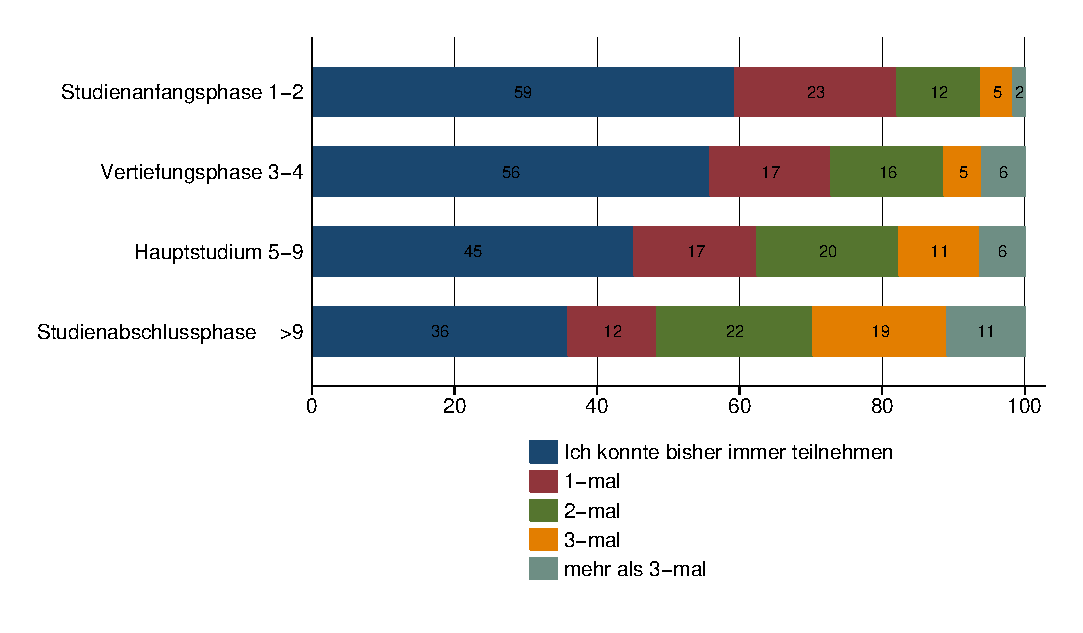
\includegraphics[
%  defaultresolution=72 !,
%  bmpsizefast=false
%]{image}
%\end{verbatim}
% \end{quote}
%
% \subsubsection{Hints}
%
% \begin{itemize}
% \item My version of \xfile{dvips.def} 1999/02/16 v3.0i defines
%       rules for the supported bitmap extensions, but does not
%       include them in the list of extensions that are tried
%       if the file name is not given with an extension.
%       In such a case, the list of extensions can be set
%       by \cs{DeclareGraphicsExtensions}, see \xpackage{grfguide}.
%       The following code just extends the list:
%       \begin{quote}
%\begin{verbatim}
%\makeatletter
%\g@addto@macro\Gin@extensions{,.bmp,.pcx,.msp}
%\makeatother
%\end{verbatim}
%       \end{quote}
% \item My version of \xfile{dvipdfm.def} 1998/11/24 vx.x misses
%       the graphics rule for PNG files. It can be added by:
%       \begin{quote}
%\begin{verbatim}
%\DeclareGraphicsRule{.png}{bmp}{.bb}{#1}
%\end{verbatim}
%       \end{quote}
%       See the previous issue to add the extension \xfile{.png} to the list
%       of extensions for package \xpackage{graphics}.
% \end{itemize}
%
% \subsubsection{Test program}
%
% There is a test program \xfile{bmpsize-test.tex}. Run it through
% \verb|latex|, \verb|pdflatex|, or \verb|pdftex|. Then given
% image files are inspected and the result is printed.
%
% \subsubsection{Interface for programmers}
%
% The macro names of the parsers are \verb|\bmpsize@read@|\meta{type}.
% Example: \cs{bmpsize@read@jpg} in case of JPEG.
%
% A parser sets the switch \cs{ifbmpsize@ok} to true, if it
% could successfully parse the image file.
% The width and height are returnd in \cs{bmpsize@width} and
% \cs{bmpsize@height}. If information about density is available,
% it is used to calculate width and height of the image, otherwise
% the values given by option \xoption{defaultresolution} is used.
% \xoption{resolution} overwrites the values in the image file.
%
% \subsection{Improved bitmap inclusion}
%
% Some drivers for package \xpackage{graphics} define the graphics
% type \xoption{bmp} for bitmap images. The code in the standard
% drivers for \xoption{dvips}, \xoption{dvipdfm}, and \xoption{dvipdfmx}
% is very basic and misses essential features of the
% package \xpackage{graphicx}. Therefore the code for bitmap
% inclusion is automatically rewritten by this package to add
% the following features:
% \begin{itemize}
% \item Support for \xoption{viewport} and \xoption{trim}.
% \item Support for \xoption{clip}.
% \item In case of \xoption{dvipdfm} and \xoption{dvipdfmx} the
%       bitmap images are reused and not included again if they
%       are used more than once.
% \end{itemize}
% However, there is a difference between \xoption{dvipdfm} and
% \xoption{dvipdfmx}, especially if images are reused. In the
% former case the reused box has width and height of 1bp, in the
% latter case its natural width. Thus the correct driver option must be given.
% \xoption{dvipdfm} and \xoption{dvipdfmx} are not equivalent.
%
% Older versions of \xoption{dvipdfmx} uses a size of 1in. However I do
% want to distinguish between versions of the same program. Therefore the
% support of these older versions has stopped with version 1.6 of this package.
% Use version dvipdfmx-20090708 or newer (some few versions before will
% probably also work, but I don't want to investigate this further).
%
% \StopEventually{
% }
%
% \section{Implementation}
%
% \subsection{Basic package \xpackage{bmpsize-base}}
%
%    Identification.
%    \begin{macrocode}
%<*base>
\ProvidesPackage{bmpsize-base}%
  [2009/09/04 v1.6 Basic part of bmpsize (HO)]%
%    \end{macrocode}
%    Modules of package \xpackage{fp} are used for calculations.
%    \begin{macrocode}
\RequirePackage{fp-basic}
\RequirePackage{fp-snap}
%    \end{macrocode}
%    Package \xpackage{fp} uses nested \cs{loop} structures.
%    That breaks with the plain-\TeX\ version of \cs{loop}.
%    Therefore we use the \LaTeX\ variant.
%    \begin{macro}{\@bmpsize@plain@loop}
%    \begin{macrocode}
\long\def\@bmpsize@plain@loop#1\repeat{%
  \def\iterate{%
    #1\relax
    \expandafter\iterate\fi
  }%
  \iterate
  \let\iterate\relax
}
%    \end{macrocode}
%    \end{macro}
%    \begin{macrocode}
\RequirePackage{pdftexcmds}[2007/11/11]
%    \end{macrocode}
%    \begin{macrocode}
\newif\ifbmpsize@ok
\let\@bmpsize@ok\bmpsize@oktrue

\newif\if@bmpsize@bigendian
\newif\if@bmpsize@absnum
\newif\if@bmpsize@user@resolution
\newif\if@bmpsize@fast
\@bmpsize@fasttrue

\def\@bmpsize@init{%
  \let\@bmpsize@org@plain@loop\loop
  \let\loop\@bmpsize@plain@loop
  \bmpsize@okfalse
  \@bmpsize@bigendiantrue
  \@bmpsize@absnumfalse
  \let\bmpsize@pixelwidth\relax
  \let\bmpsize@pixelheight\relax
  \let\bmpsize@pixelx\relax
  \let\bmpsize@pixely\relax
  \let\bmpsize@unit\relax
  \let\bmpsize@pixelxdenom\relax
  \let\bmpsize@pixelydenom\relax
  \let\bmpsize@orientation\relax
}

\def\@bmpsize@stop#1\@nil{}

\def\@bmpsize@loop#1{%
  #1%
  \@bmpsize@loop{#1}%
}
\def\@bmpsize@break#1\@bmpsize@loop#2{}

\def\@bmpsize@size#1#2#3{%
  \edef#3{\pdf@filesize{#1}}%
  \ifx#3\@empty
    \expandafter\@bmpsize@stop
  \fi
  \ifnum#3<#2\relax
    \expandafter\@bmpsize@stop
  \fi
}

\def\@bmpsize@read#1#2#3{%
  \edef\@bmpsize@buf{\pdf@filedump{#3}{#2}{#1}}%
  \edef\@bmpsize@temp{%
    \noexpand\@bmpsize@check@byte{#2}\@bmpsize@buf{}{}\noexpand\\%
  }%
  \@bmpsize@temp
}
\def\@bmpsize@fillbuf#1{%
  \ifx\@bmpsize@buf\@empty
    \expandafter\@firstofone
  \else
    \expandafter\@gobble
  \fi
  {%
    \edef\@bmpsize@buf{%
      \pdf@filedump{\bmpsize@offset}{\bmpsize@fillbuflength}{#1}%
    }%
    \ifx\@bmpsize@buf\@empty
      \expandafter\@bmpsize@stop
    \fi
    \edef\bmpsize@offset{\the\numexpr\bmpsize@offset+\bmpsize@fillbuflength}%
  }%
}
\def\bmpsize@fillbuflength{10}

\def\@bmpsize@append#1#2#3{%
  \edef#1{#2#3}%
}
\def\@bmpsize@pushback#1{%
  \edef\@bmpsize@buf{#1\@bmpsize@buf}%
}

\def\@bmpsize@iswhite#1{%
  \ifnum\pdf@strcmp{#1}{09}=\z@
  \else
    \ifnum\pdf@strcmp{#1}{0A}=\z@
    \else
      \ifnum\pdf@strcmp{#1}{0D}=\z@
      \else
        \ifnum\pdf@strcmp{#1}{20}=\z@
        \else
          1%
        \fi
      \fi
    \fi
  \fi
  \space
}
\def\@bmpsize@isdigit#1{%
  \ifnum\pdf@strcmp{#1}{30}<\z@
    1%
  \else
    \ifnum\pdf@strcmp{#1}{39}>\z@
      1%
    \fi
  \fi
  \space
}

\def\@bmpsize@check@byte#1#2#3{%
  \ifnum#1<\@ne
    \csname fi\endcsname
    \@bmpsize@cleanup@end
  \else
    \csname fi\endcsname
  \ifx!#2#3!%
    \csname fi\endcsname
    \@bmpsize@stop
  \else
    \csname fi\endcsname
    \expandafter\@bmpsize@check@byte\expandafter{\the\numexpr#1-1}%
}
\def\@bmpsize@cleanup@end#1\\{}

\def\@bmpsize@swap@maybe#1{%
  \if@bmpsize@bigendian
  \else
    \edef#1{\expandafter\@bmpsize@@swap#1\@empty\@empty\@empty\@empty}%
  \fi
}
\def\@bmpsize@@swap#1#2#3#4#5#6#7#8{%
  #7#8#5#6#3#4#1#2%
}

\def\@bmpsize@skip@one{%
  \edef\@bmpsize@buf{\expandafter\@gobbletwo\@bmpsize@buf}%
}
\def\@bmpsize@skip@two{%
  \edef\@bmpsize@buf{\expandafter\@gobblefour\@bmpsize@buf}%
}
\def\@bmpsize@skip@four{%
  \edef\@bmpsize@buf{%
    \expandafter\expandafter\expandafter\@gobblefour\expandafter
    \@gobblefour\@bmpsize@buf
  }%
}

\def\@bmpsize@grab#1#2{%
  \edef#1{\noexpand\@bmpsize@grab@byte#2=\@bmpsize@buf\noexpand\\}%
  \edef#1{#1}%
}
\def\@bmpsize@grab@byte#1=#2#3{%
  #2#3%
  \ifnum#1>\@ne
    \expandafter\@bmpsize@grab@byte\the\numexpr#1-1\expandafter=%
  \else
    \expandafter\@bmpsize@cleanup@end
  \fi
}

\def\@bmpsize@abs@maybe#1{%
  \let\@bmpsize@temp\relax
  \if@bmpsize@absnum
    \ifnum"\expandafter\@car#1\@nil>7 %
      \edef#1{\expandafter\@bmpsize@abs@byte#1\relax}%
      \ifnum\pdf@strcmp{#1}{7FFFFFFF}=\z@
        \let\@bmpsize@temp\@bmpsize@stop
      \else
        \def\@bmpsize@temp{\edef#1{\the\numexpr#1+1}}%
      \fi
    \fi
  \fi
}
\def\@bmpsize@abs@byte#1{%
  \ifx#1\relax
  \else
    \ifcase"0#1 %
      F\or E\or D\or C\or B\or A\or 9\or 8\or
      7\or 6\or 5\or 4\or 3\or 2\or 1\or 0%
    \fi
    \expandafter\@bmpsize@abs@byte
  \fi
}

\def\@bmpsize@num@one#1{%
  \@bmpsize@grab#11%
  \@bmpsize@abs@maybe#1%
  \edef#1{\number"#1}%
  \@bmpsize@temp
  \@bmpsize@skip@one
}
\def\@bmpsize@num@two#1{%
  \@bmpsize@grab#12%
  \@bmpsize@swap@maybe#1%
  \@bmpsize@abs@maybe#1%
  \edef#1{\number"#1}%
  \@bmpsize@temp
  \@bmpsize@skip@two
}
\def\@bmpsize@num@four#1{%
  \@bmpsize@grab#14%
  \@bmpsize@swap@maybe#1%
  \@bmpsize@abs@maybe#1%
  \ifnum\pdf@strcmp{#1}{7FFFFFFF}>\z@
    \expandafter\@bmpsize@stop
  \fi
  \edef#1{\number"#1}%
  \@bmpsize@temp
  \@bmpsize@skip@four
}

\def\@bmpsize@div#1#2#3{% #1 := #2/#3
  \FPdiv#1{#2}{#3}%
  \@bmpsize@beautify#1%
}
\def\@bmpsize@beautify#1{%
  \FPifint#1%
    \edef#1{\expandafter\@bmpsize@trunc#1.\@nil}%
  \else
    \edef#1{\expandafter\@bmpsize@cleanup@frac#1.\@nil}%
  \fi
}
\def\@bmpsize@trunc#1.#2\@nil{#1}
% #1 isn't an integer, thus we should have at least one
% necessary digit after the dot
\def\@bmpsize@cleanup@frac#1.#2#3.#4\@nil{%
  #1.#2%
  \ifx\\#3\\%
  \else
    \@bmpsize@cleanup@fracdigits#3000000000\@nil
  \fi
}
\def\@bmpsize@cleanup@fracdigits#1#2#3#4#5#6#7#8#9{%
  \ifcase#9 %
    \ifcase#8 %
      \ifcase#7 %
        \ifcase#6 %
          \ifcase#5 %
            \ifcase #4 %
              \ifcase #3 %
                \ifcase #2 %
                  \ifcase #1 %
                  \else
                    #1%
                  \fi
                \else
                  #1#2%
                \fi
              \else
                #1#2#3%
              \fi
            \else
              #1#2#3#4%
            \fi
          \else
            #1#2#3#4#5%
          \fi
        \else
          #1#2#3#4#5#6%
        \fi
      \else
        #1#2#3#4#5#6#7%
      \fi
    \else
      #1#2#3#4#5#6#7#8%
    \fi
  \else
    #1#2#3#4#5#6#7#8#9%
  \fi
  \@bmpsize@trunc.%
}

\def\@bmpsize@end{%
  \ifbmpsize@ok
    \ifx\bmpsize@pixelwidth\relax
      \bmpsize@okfalse
    \fi
    \ifx\bmpsize@pixelheight\relax
      \bmpsize@okfalse
    \fi
  \fi
  \ifbmpsize@ok
    \ifnum\bmpsize@pixelwidth>\z@
    \else
      \bmpsize@okfalse
    \fi
    \ifnum\bmpsize@pixelheight>\z@
    \else
      \bmpsize@okfalse
    \fi
  \fi
  \ifbmpsize@ok
    \ifcase 0%
      \ifx\bmpsize@pixelx\relax 1 \fi
      \ifx\bmpsize@pixely\relax 1 \fi
      \ifnum\bmpsize@pixelx>\z@\else 1 \fi
      \ifnum\bmpsize@pixely>\z@\else 1 \fi
      \ifx\bmpsize@pixelxdenom\relax
         \ifx\bmpsize@pixelydenom\relax\else 1 \fi
      \else
        \ifnum\bmpsize@pixelxdenom>\z@\else 1 \fi
      \fi
      \ifx\bmpsize@pixelydenom\relax
      \else
        \ifnum\bmpsize@pixelydenom>\z@\else 1 \fi
      \fi
    \else
      \let\bmpsize@pixelx\relax
      \let\bmpsize@pixely\relax
      \let\bmpsize@unit\relax
      \let\bmpsize@pixelxdenom\relax
      \let\bmpsize@pixelydenom\relax
    \fi
    \ifx\bmpsize@pixelxdenom\relax
    \else
      \@bmpsize@div\bmpsize@pixelx\bmpsize@pixelx\bmpsize@pixelxdenom
      \@bmpsize@div\bmpsize@pixely\bmpsize@pixely\bmpsize@pixelydenom
      \let\bmpsize@pixelxdenom\relax
      \let\bmpsize@pixelydenom\relax
    \fi
    \ifcase 0\ifx\bmpsize@unit\relax 1\fi
             \if@bmpsize@user@resolution 1\fi
             \relax
      \let\bmpsize@calc@unit\bmpsize@unit
      \let\bmpsize@calc@pixelx\bmpsize@pixelx
      \let\bmpsize@calc@pixely\bmpsize@pixely
    \else
      \let\bmpsize@calc@unit\bmpsize@unit@default
      \let\bmpsize@calc@pixelx\bmpsize@pixelx@default
      \let\bmpsize@calc@pixely\bmpsize@pixely@default
      \ifx\bmpsize@calc@pixely\Gin@exclamation
        \ifx\bmpsize@pixelx\relax
          \let\bmpsize@calc@pixely\bmpsize@calc@pixelx
        \else
          \FPdiv\bmpsize@calc@pixely\bmpsize@calc@pixelx\bmpsize@pixelx
          \FPmul\bmpsize@calc@pixely\bmpsize@calc@pixely\bmpsize@pixely
        \fi
      \else
        \ifx\bmpsize@calc@pixelx\Gin@exclamation
          \ifx\bmpsize@pixelx\relax
            \let\bmpsize@calc@pixelx\bmpsize@calc@pixely
          \else
            \FPdiv\bmpsize@calc@pixelx\bmpsize@calc@pixely\bmpsize@pixely
            \FPmul\bmpsize@calc@pixelx\bmpsize@calc@pixelx\bmpsize@pixelx
          \fi
        \fi
      \fi
    \fi
    \FPdiv\bmpsize@width\bmpsize@pixelwidth\bmpsize@calc@pixelx
    \FPdiv\bmpsize@height\bmpsize@pixelheight\bmpsize@calc@pixely
    % calculation of width and height in bp for package graphics
    % 1in = 72bp = 72.27pt, 72/72.27 = 8/8.03, 1pt = 65536sp
    \if@bmpsize@fast
      \edef\bmpsize@width{%
        \strip@pt\dimexpr.99626\dimexpr
        \bmpsize@width\dimexpr\bmpsize@calc@unit
      }%
      \edef\bmpsize@height{%
        \strip@pt\dimexpr.99626\dimexpr
        \bmpsize@height\dimexpr\bmpsize@calc@unit
      }%
    \else
      \edef\@bmpsize@temp{\number\dimexpr\bmpsize@calc@unit}%
      \ifnum\@bmpsize@temp>100000 %
        \FPmul\@bmpsize@temp\@bmpsize@temp{0.00001}%
        \def\@bmpsize@corr{100000}%
      \else
        \let\@bmpsize@corr\relax
      \fi
      \FPmul\bmpsize@width\bmpsize@width\@bmpsize@temp
      \FPmul\bmpsize@height\bmpsize@height\@bmpsize@temp
      \FPmul\bmpsize@width\bmpsize@width{8}%
      \FPmul\bmpsize@height\bmpsize@height{8}%
      \FPdiv\bmpsize@width\bmpsize@width{8.03}%
      \FPdiv\bmpsize@height\bmpsize@height{8.03}%
      \FPdiv\bmpsize@width\bmpsize@width{65536}%
      \FPdiv\bmpsize@height\bmpsize@height{65536}%
      \ifx\@bmpsize@corr\relax
      \else
        \FPmul\bmpsize@width\bmpsize@width\@bmpsize@corr
        \FPmul\bmpsize@height\bmpsize@height\@bmpsize@corr
      \fi
      \FPround\bmpsize@width\bmpsize@width{5}%
      \FPround\bmpsize@height\bmpsize@height{5}%
      \@bmpsize@beautify\bmpsize@width
      \@bmpsize@beautify\bmpsize@height
    \fi
  \fi
  \let\loop\@bmpsize@org@plain@loop
}
\def\bmpsize@unit@default{72.27pt}% more accurate than 1in
\def\bmpsize@pixelx@default{72}
\let\bmpsize@pixely@default\Gin@exclamation

\def\bmpsize@types{png,jpg,bmp,gif,tiff,pnm,pam,xpm,tga,pcx,msp,sgi}
%</base>
%    \end{macrocode}
%
% \subsection{Bitmap formats}
%
% \subsubsection{png}
%
%\iffalse
%<*ignore>
%\fi
%\begin{verbatim}
%begin png
%big-endian
%
%read 24 0
%grab 8        -> $temp
%check streq $temp [0x89 "PNG" 0x0D 0x0A 0x1A 0x0A]
%num 4         -> $length
%grab 4        -> $temp
%check streq $temp ["IHDR"]
%num 4         -> $pixelwidth
%num 4         -> $pixelheight
%ok
%assign numexpr(20 + $length) -> $offset
%loop
%  read 8 $offset
%  num 4       -> $length
%  grab 4      -> $temp
%  if streq $temp ["IDAT"]
%    stop
%  fi
%  if streq $temp ["pHYs"]
%    read 9 numexpr($offset + 8)
%    num 4     -> $pixelx
%    num 4     -> $pixely
%    grab 1     -> $temp
%    if numeq $temp 1
%      assign {100cm} -> $unit
%    fi
%    stop
%  fi
%  assign numexpr($offset + 12 + $length) -> $offset
%repeat
%end
%\end{verbatim}
%\iffalse
%</ignore>
%\fi
%    \begin{macro}{\bmpsize@read@png}
%    \begin{macrocode}
%<*base>
\def\bmpsize@read@png#1{%
  \@bmpsize@init
  \@bmpsize@bigendiantrue
  \@bmpsize@read{#1}{24}{0}%
  \@bmpsize@grab\bmpsize@temp{8}%
  \@bmpsize@skip@four
  \@bmpsize@skip@four
  \ifnum\pdf@strcmp{\bmpsize@temp}{89504E470D0A1A0A}=\z@
  \else
    \expandafter\@bmpsize@stop
  \fi
  \@bmpsize@num@four\bmpsize@length
  \@bmpsize@grab\bmpsize@temp{4}%
  \@bmpsize@skip@four
  \ifnum\pdf@strcmp{\bmpsize@temp}{49484452}=\z@
  \else
    \expandafter\@bmpsize@stop
  \fi
  \@bmpsize@num@four\bmpsize@pixelwidth
  \@bmpsize@num@four\bmpsize@pixelheight
  \@bmpsize@ok
  \edef\bmpsize@offset{\the\numexpr20+\bmpsize@length}%
  \@bmpsize@loop{%
    \@bmpsize@read{#1}{8}{\bmpsize@offset}%
    \@bmpsize@num@four\bmpsize@length
    \@bmpsize@grab\bmpsize@temp{4}%
    \@bmpsize@skip@four
    \ifnum\pdf@strcmp{\bmpsize@temp}{49444154}=\z@
      \expandafter\@firstofone
    \else
      \expandafter\@gobble
    \fi
    {%
      \@bmpsize@stop
    }%
    \ifnum\pdf@strcmp{\bmpsize@temp}{70485973}=\z@
      \expandafter\@firstofone
    \else
      \expandafter\@gobble
    \fi
    {%
      \@bmpsize@read{#1}{9}{\numexpr\bmpsize@offset+8\relax}%
      \@bmpsize@num@four\bmpsize@pixelx
      \@bmpsize@num@four\bmpsize@pixely
      \@bmpsize@grab\bmpsize@temp{1}%
      \@bmpsize@skip@one
      \ifnum\bmpsize@temp=1\relax
        \expandafter\@firstofone
      \else
        \expandafter\@gobble
      \fi
      {%
        \def\bmpsize@unit{100cm}%
      }%
      \@bmpsize@stop
    }%
    \edef\bmpsize@offset{\the\numexpr\bmpsize@offset+12+\bmpsize@length}%
  }%
  \@bmpsize@stop
  \@nil
  \@bmpsize@end
}%
%</base>
%    \end{macrocode}
%    \end{macro}
%
% \subsubsection{jpg}
%
%\iffalse
%<*ignore>
%\fi
%\begin{verbatim}
%begin jpg
%
%read 3 0
%grab 3      -> $temp % SOI and 0xFF
%check streq $temp [0xFF 0xD8 0xFF]
%assign {2} -> $offset
%assign {0} -> $exifdensity
%loop
%  read 4 $offset
%  grab 1    -> $temp
%  check streq $temp [0xFF]
%  num 1    -> $temp
%  if numeq $temp 0xDA % SOS
%    stop
%  fi
%  % look for JFIF APP0 segment
%  if numeq $temp 0xE0 % APP0
%    num 2       -> $length
%    if numeq $exifdensity 0
%      if numge $length 16 % a JFIF segment has 16 bytes at least
%        read 12 numexpr($offset + 4)
%        grab 5      -> $temp % identifier
%        if streq $temp ["JFIF" 0x0]
%          check numge $length 16
%          skip 2 % version
%          num 1       -> $temp % units
%          if numeq $temp 1
%            assign {72.27pt} -> $unit
%          else
%            if numeq $temp 2
%              assign {1cm} -> $unit
%            fi
%          fi
%          num 2    -> $pixelx
%          num 2    -> $pixely
%        fi
%      fi
%    fi
%  else
%    if numeq $temp 0xE1 % APP1
%      % look for Exif APP1 segment
%      num 2 -> $length
%      if numge $length 20 % identifier (6) + Tiff header (8) + first IFD (>=6)
%        read 20 numexpr($offset + 4)
%        grab 6 -> $temp
%        if streq $temp ["Exif" 0x0 0x0]
%          assign numexpr($offset + 10) -> $exifoffset
%          % read TIFF header
%          grab 2 -> $temp
%          if streq $temp ["II"]
%            little-endian
%          else
%            check streq $temp ["MM"]
%            % big-endian
%          fi
%          num 2 -> $temp
%          check numeq $temp 42
%          num 4 -> $temp % offset of first IFD
%          check numgt $temp 0
%          % read first IFD
%          assign numexpr($temp + $exifoffset) -> $off
%          read 2 $off
%          num 2 -> $entries
%          assign numexpr($off + 2) -> $off
%          loop
%            if numeq $entries 0
%              break
%            fi
%            assign numexpr($entries - 1) -> $entries
%            % entry format:
%            % 2 tag
%            % 2 field type
%            % 4 count
%            % 4 value/offset
%            read 12 $off
%            assign numexpr($off + 12) -> $off
%            num 2 -> $tag
%            if numeq $tag 296 % ResolutionUnit
%              skip 6 % type: 3 (short), count: 1
%              num 2 -> $temp
%              ifcase $temp
%              or % 1
%                clear $unit
%              or % 2
%                assign {72.27pt} -> $unit
%              or % 3
%                assign {1cm} -> $unit
%              else
%                clear $unit % unknown
%              fi
%              ifcase $temp
%              or % 1
%              or % 2
%                assign {1} -> $exifdensity
%              or % 3
%                assign {1} -> $exifdensity
%              else
%                assign $exifdensity -> $exifdensity
%              fi
%            fi
%            % 256 ImageWidth (use width of JPG part)
%            % 257 ImageHeight (use height of JPG part)
%            if numeq $tag 274 % Orientation
%              skip 6 % type: 3 (short), count: 1
%              num 2 -> $temp
%              if numge $temp 0 
%                if numle $temp 8
%                  assign $temp -> $orientation
%                fi
%              fi
%            fi
%            if numeq $tag 282 % XResolution
%              skip 6
%              num 4 -> $temp
%              read 8 numexpr($temp + $exifoffset)
%              num 4 -> $pixelx
%              num 4 -> $temp
%              if numeq $temp 1
%              else
%                assign numexpr($temp) -> $pixelxdenom
%                % div $pixelx $temp -> $pixelx
%              fi
%            fi
%            if numeq $tag 283 % YResolution
%              skip 6
%              num 4 -> $temp
%              read 8 numexpr($temp + $exifoffset)
%              num 4 -> $pixely
%              num 4 -> $temp
%              if numeq $temp 1
%              else
%                assign numexpr($temp) -> $pixelydenom
%                % div $pixely $temp -> $pixely
%              fi
%            fi
%          repeat
%          big-endian
%        fi
%      fi
%    else
%      assign numexpr($temp - 0xC0) -> $temp
%      ifcase $temp % SOF_0
%      or % SOF_1
%      or % SOF_2
%      or % SOF_3
%      or % DHT
%        assign {-1} -> $temp
%      or % SOF_5
%      or % SOF_6
%      or % SOF_7
%      or % JPG
%        assign {-1} -> $temp
%      or % SOF_9
%      or % SOF_10
%      or % SOF_11
%      or % DAC
%        assign {-1} -> $temp
%      or % SOF_13
%      or % SOF_14
%      or % SOF_15
%      else
%        assign {-1} -> $temp
%      fi
%      if numeq $temp -1
%      else
%        read 4 numexpr($offset + 5)
%        num 2  -> $pixelheight
%        num 2  -> $pixelwidth
%        if numeq $pixelheight 0
%          clear $pixelheight
%          stop
%        fi
%        ok
%        stop
%      fi
%      num 2 -> $length
%    fi
%  fi
%  assign numexpr($offset + $length + 2) -> $offset
%repeat
%end
%\end{verbatim}
%\iffalse
%</ignore>
%\fi
%    \begin{macro}{\bmpsize@read@jpg}
%    \begin{macrocode}
%<*base>
\def\bmpsize@read@jpg#1{%
  \@bmpsize@init
  \@bmpsize@read{#1}{3}{0}%
  \@bmpsize@grab\bmpsize@temp{3}%
  \@bmpsize@skip@two
  \@bmpsize@skip@one
  \ifnum\pdf@strcmp{\bmpsize@temp}{FFD8FF}=\z@
  \else
    \expandafter\@bmpsize@stop
  \fi
  \def\bmpsize@offset{2}%
  \def\bmpsize@exifdensity{0}%
  \@bmpsize@loop{%
    \@bmpsize@read{#1}{4}{\bmpsize@offset}%
    \@bmpsize@grab\bmpsize@temp{1}%
    \@bmpsize@skip@one
    \ifnum\pdf@strcmp{\bmpsize@temp}{FF}=\z@
    \else
      \expandafter\@bmpsize@stop
    \fi
    \@bmpsize@num@one\bmpsize@temp
    \ifnum\bmpsize@temp=218\relax
      \expandafter\@firstofone
    \else
      \expandafter\@gobble
    \fi
    {%
      \@bmpsize@stop
    }%
    \ifnum\bmpsize@temp=224\relax
      \expandafter\@firstoftwo
    \else
      \expandafter\@secondoftwo
    \fi
    {%
      \@bmpsize@num@two\bmpsize@length
      \ifnum\bmpsize@exifdensity=0\relax
        \expandafter\@firstofone
      \else
        \expandafter\@gobble
      \fi
      {%
        \unless\ifnum\bmpsize@length<16\relax
          \expandafter\@firstofone
        \else
          \expandafter\@gobble
        \fi
        {%
          \@bmpsize@read{#1}{12}{\numexpr\bmpsize@offset+4\relax}%
          \@bmpsize@grab\bmpsize@temp{5}%
          \@bmpsize@skip@four
          \@bmpsize@skip@one
          \ifnum\pdf@strcmp{\bmpsize@temp}{4A46494600}=\z@
            \expandafter\@firstofone
          \else
            \expandafter\@gobble
          \fi
          {%
            \ifnum\bmpsize@length<16\relax
              \expandafter\@bmpsize@stop
            \fi
            \@bmpsize@skip@two
            \@bmpsize@num@one\bmpsize@temp
            \ifnum\bmpsize@temp=1\relax
              \expandafter\@firstoftwo
            \else
              \expandafter\@secondoftwo
            \fi
            {%
              \def\bmpsize@unit{72.27pt}%
            }{%
              \ifnum\bmpsize@temp=2\relax
                \expandafter\@firstofone
              \else
                \expandafter\@gobble
              \fi
              {%
                \def\bmpsize@unit{1cm}%
              }%
            }%
            \@bmpsize@num@two\bmpsize@pixelx
            \@bmpsize@num@two\bmpsize@pixely
          }%
        }%
      }%
    }{%
      \ifnum\bmpsize@temp=225\relax
        \expandafter\@firstoftwo
      \else
        \expandafter\@secondoftwo
      \fi
      {%
        \@bmpsize@num@two\bmpsize@length
        \unless\ifnum\bmpsize@length<20\relax
          \expandafter\@firstofone
        \else
          \expandafter\@gobble
        \fi
        {%
          \@bmpsize@read{#1}{20}{\numexpr\bmpsize@offset+4\relax}%
          \@bmpsize@grab\bmpsize@temp{6}%
          \@bmpsize@skip@four
          \@bmpsize@skip@two
          \ifnum\pdf@strcmp{\bmpsize@temp}{457869660000}=\z@
            \expandafter\@firstofone
          \else
            \expandafter\@gobble
          \fi
          {%
            \edef\bmpsize@exifoffset{\the\numexpr\bmpsize@offset+10}%
            \@bmpsize@grab\bmpsize@temp{2}%
            \@bmpsize@skip@two
            \ifnum\pdf@strcmp{\bmpsize@temp}{4949}=\z@
              \expandafter\@firstoftwo
            \else
              \expandafter\@secondoftwo
            \fi
            {%
              \@bmpsize@bigendianfalse
            }{%
              \ifnum\pdf@strcmp{\bmpsize@temp}{4D4D}=\z@
              \else
                \expandafter\@bmpsize@stop
              \fi
            }%
            \@bmpsize@num@two\bmpsize@temp
            \ifnum\bmpsize@temp=42\relax
            \else
              \expandafter\@bmpsize@stop
            \fi
            \@bmpsize@num@four\bmpsize@temp
            \ifnum\bmpsize@temp>0\relax
            \else
              \expandafter\@bmpsize@stop
            \fi
            \edef\bmpsize@off{\the\numexpr\bmpsize@temp+\bmpsize@exifoffset}%
            \@bmpsize@read{#1}{2}{\bmpsize@off}%
            \@bmpsize@num@two\bmpsize@entries
            \edef\bmpsize@off{\the\numexpr\bmpsize@off+2}%
            \@bmpsize@loop{%
              \ifnum\bmpsize@entries=0\relax
                \expandafter\@firstofone
              \else
                \expandafter\@gobble
              \fi
              {%
                \@bmpsize@break
              }%
              \edef\bmpsize@entries{\the\numexpr\bmpsize@entries-1}%
              \@bmpsize@read{#1}{12}{\bmpsize@off}%
              \edef\bmpsize@off{\the\numexpr\bmpsize@off+12}%
              \@bmpsize@num@two\bmpsize@tag
              \ifnum\bmpsize@tag=296\relax
                \expandafter\@firstofone
              \else
                \expandafter\@gobble
              \fi
              {%
                \@bmpsize@skip@four
                \@bmpsize@skip@two
                \@bmpsize@num@two\bmpsize@temp
                \ifcase\bmpsize@temp\relax
                \or
                  \let\bmpsize@unit\relax
                \or
                  \def\bmpsize@unit{72.27pt}%
                \or
                  \def\bmpsize@unit{1cm}%
                \else
                  \let\bmpsize@unit\relax
                \fi
                \ifcase\bmpsize@temp\relax
                \or
                \or
                  \def\bmpsize@exifdensity{1}%
                \or
                  \def\bmpsize@exifdensity{1}%
                \else
                  \let\bmpsize@exifdensity\bmpsize@exifdensity
                \fi
              }%
              \ifnum\bmpsize@tag=274\relax
                \expandafter\@firstofone
              \else
                \expandafter\@gobble
              \fi
              {%
                \@bmpsize@skip@four
                \@bmpsize@skip@two
                \@bmpsize@num@two\bmpsize@temp
                \unless\ifnum\bmpsize@temp<0\relax
                  \expandafter\@firstofone
                \else
                  \expandafter\@gobble
                \fi
                {%
                  \unless\ifnum\bmpsize@temp>8\relax
                    \expandafter\@firstofone
                  \else
                    \expandafter\@gobble
                  \fi
                  {%
                    \let\bmpsize@orientation\bmpsize@temp
                  }%
                }%
              }%
              \ifnum\bmpsize@tag=282\relax
                \expandafter\@firstofone
              \else
                \expandafter\@gobble
              \fi
              {%
                \@bmpsize@skip@four
                \@bmpsize@skip@two
                \@bmpsize@num@four\bmpsize@temp
                \@bmpsize@read{#1}{8}{\numexpr\bmpsize@temp+\bmpsize@exifoffset\relax}%
                \@bmpsize@num@four\bmpsize@pixelx
                \@bmpsize@num@four\bmpsize@temp
                \ifnum\bmpsize@temp=1\relax
                  \expandafter\@gobble
                \else
                  \expandafter\@firstofone
                \fi
                {%
                  \edef\bmpsize@pixelxdenom{\the\numexpr\bmpsize@temp}%
                }%
              }%
              \ifnum\bmpsize@tag=283\relax
                \expandafter\@firstofone
              \else
                \expandafter\@gobble
              \fi
              {%
                \@bmpsize@skip@four
                \@bmpsize@skip@two
                \@bmpsize@num@four\bmpsize@temp
                \@bmpsize@read{#1}{8}{\numexpr\bmpsize@temp+\bmpsize@exifoffset\relax}%
                \@bmpsize@num@four\bmpsize@pixely
                \@bmpsize@num@four\bmpsize@temp
                \ifnum\bmpsize@temp=1\relax
                  \expandafter\@gobble
                \else
                  \expandafter\@firstofone
                \fi
                {%
                  \edef\bmpsize@pixelydenom{\the\numexpr\bmpsize@temp}%
                }%
              }%
            }%
            \@bmpsize@bigendiantrue
          }%
        }%
      }{%
        \edef\bmpsize@temp{\the\numexpr\bmpsize@temp-192}%
        \ifcase\bmpsize@temp\relax
        \or
        \or
        \or
        \or
          \def\bmpsize@temp{-1}%
        \or
        \or
        \or
        \or
          \def\bmpsize@temp{-1}%
        \or
        \or
        \or
        \or
          \def\bmpsize@temp{-1}%
        \or
        \or
        \or
        \else
          \def\bmpsize@temp{-1}%
        \fi
        \ifnum\bmpsize@temp=-1\relax
          \expandafter\@gobble
        \else
          \expandafter\@firstofone
        \fi
        {%
          \@bmpsize@read{#1}{4}{\numexpr\bmpsize@offset+5\relax}%
          \@bmpsize@num@two\bmpsize@pixelheight
          \@bmpsize@num@two\bmpsize@pixelwidth
          \ifnum\bmpsize@pixelheight=0\relax
            \expandafter\@firstofone
          \else
            \expandafter\@gobble
          \fi
          {%
            \let\bmpsize@pixelheight\relax
            \@bmpsize@stop
          }%
          \@bmpsize@ok
          \@bmpsize@stop
        }%
        \@bmpsize@num@two\bmpsize@length
      }%
    }%
    \edef\bmpsize@offset{\the\numexpr\bmpsize@offset+\bmpsize@length+2}%
  }%
  \@bmpsize@stop
  \@nil
  \@bmpsize@end
}%
%</base>
%    \end{macrocode}
%    \end{macro}
%
% \subsubsection{bmp}
%
%\iffalse
%<*ignore>
%\fi
%\begin{verbatim}
%begin bmp
%little-endian
%
%read 26 0
%grab 2 -> $temp
%check streq $temp ["BM"]
%skip 12
%% header size is 4 bytes in V3+, unknown for V1, V2,
%% known header sizes fit in 2 bytes
%num 2   -> $temp
%if numeq $temp 12 % V1
%  skip 2
%  num 2 -> $pixelwidth
%  num 2 -> $pixelheight
%  % no resolution entries
%  ok
%  stop
%fi
%if numeq $temp 64 % V2
%  skip 2
%  num 2 -> $pixelwidth
%  num 2 -> $pixelheight
%  % missing specification for resolution
%  ok
%  stop
%fi
%% V3, V4, V5
%skip 2
%num 4 -> $pixelwidth
%absnum 4 -> $pixelheight
%ok
%read 8 38
%num 4 -> $pixelx
%num 4 -> $pixely
%assign {100cm} -> $unit
%end
%\end{verbatim}
%\iffalse
%</ignore>
%\fi
%    \begin{macro}{\bmpsize@read@bmp}
%    \begin{macrocode}
%<*base>
\def\bmpsize@read@bmp#1{%
  \@bmpsize@init
  \@bmpsize@bigendianfalse
  \@bmpsize@read{#1}{26}{0}%
  \@bmpsize@grab\bmpsize@temp{2}%
  \@bmpsize@skip@two
  \ifnum\pdf@strcmp{\bmpsize@temp}{424D}=\z@
  \else
    \expandafter\@bmpsize@stop
  \fi
  \@bmpsize@skip@four
  \@bmpsize@skip@four
  \@bmpsize@skip@four
  \@bmpsize@num@two\bmpsize@temp
  \ifnum\bmpsize@temp=12\relax
    \expandafter\@firstofone
  \else
    \expandafter\@gobble
  \fi
  {%
    \@bmpsize@skip@two
    \@bmpsize@num@two\bmpsize@pixelwidth
    \@bmpsize@num@two\bmpsize@pixelheight
    \@bmpsize@ok
    \@bmpsize@stop
  }%
  \ifnum\bmpsize@temp=64\relax
    \expandafter\@firstofone
  \else
    \expandafter\@gobble
  \fi
  {%
    \@bmpsize@skip@two
    \@bmpsize@num@two\bmpsize@pixelwidth
    \@bmpsize@num@two\bmpsize@pixelheight
    \@bmpsize@ok
    \@bmpsize@stop
  }%
  \@bmpsize@skip@two
  \@bmpsize@num@four\bmpsize@pixelwidth
  \@bmpsize@absnumtrue
  \@bmpsize@num@four\bmpsize@pixelheight
  \@bmpsize@absnumfalse
  \@bmpsize@ok
  \@bmpsize@read{#1}{8}{38}%
  \@bmpsize@num@four\bmpsize@pixelx
  \@bmpsize@num@four\bmpsize@pixely
  \def\bmpsize@unit{100cm}%
  \@bmpsize@stop
  \@nil
  \@bmpsize@end
}%
%</base>
%    \end{macrocode}
%    \end{macro}
%
% \subsubsection{gif}
%
%\iffalse
%<*ignore>
%\fi
%\begin{verbatim}
%begin gif
%little-endian
%
%% Header
%read 13 0
%grab 3      -> $temp
%check streq $temp ["GIF"]
%skip 3      % version
%
%% Logical Screen Descriptor
%num 2       -> $pixelwidth
%num 2       -> $pixelheight
%skip 2
%num 1       -> $temp % Pixel Aspect Ratio
%if numeq $temp 0
%else
%  assign numexpr($temp + 15) -> $pixelx
%  assign {64}     -> $pixely
%fi
%ok
%end
%\end{verbatim}
%\iffalse
%</ignore>
%\fi
%    \begin{macro}{\bmpsize@read@gif}
%    \begin{macrocode}
%<*base>
\def\bmpsize@read@gif#1{%
  \@bmpsize@init
  \@bmpsize@bigendianfalse
  \@bmpsize@read{#1}{13}{0}%
  \@bmpsize@grab\bmpsize@temp{3}%
  \@bmpsize@skip@two
  \@bmpsize@skip@one
  \ifnum\pdf@strcmp{\bmpsize@temp}{474946}=\z@
  \else
    \expandafter\@bmpsize@stop
  \fi
  \@bmpsize@skip@two
  \@bmpsize@skip@one
  \@bmpsize@num@two\bmpsize@pixelwidth
  \@bmpsize@num@two\bmpsize@pixelheight
  \@bmpsize@skip@two
  \@bmpsize@num@one\bmpsize@temp
  \ifnum\bmpsize@temp=0\relax
    \expandafter\@gobble
  \else
    \expandafter\@firstofone
  \fi
  {%
    \edef\bmpsize@pixelx{\the\numexpr\bmpsize@temp+15}%
    \def\bmpsize@pixely{64}%
  }%
  \@bmpsize@ok
  \@bmpsize@stop
  \@nil
  \@bmpsize@end
}%
%</base>
%    \end{macrocode}
%    \end{macro}
%
% \subsubsection{tiff}
%
%\iffalse
%<*ignore>
%\fi
%\begin{verbatim}
%begin tiff
%% defaults
%assign {72.27pt} -> $unit
%
%% Image File Header
%read 8 0
%grab 2 -> $temp
%if streq $temp ["II"]
%  little-endian
%else
%  check streq $temp ["MM"]
%  big-endian
%fi
%num 2 -> $temp
%check numeq $temp 42
%num 4 -> $offset % first IFD (Image File Directory)
%
%% First IFD
%read 2 $offset
%assign numexpr($offset + 2) -> $offset
%num 2 -> $entries
%ok % must rely on checks at the end
%loop
%  if numeq $entries 0
%    stop
%  fi
%  assign numexpr($entries - 1) -> $entries
%  % entry format:
%  % 2 tag
%  % 2 field type
%  % 4 count
%  % 4 value/offset
%  read 12 $offset
%  assign numexpr($offset + 12) -> $offset
%  num 2 -> $tag % tag
%  if numeq $temp 296 % ResolutionUnit
%    skip 6 % type: 3 (short), count: 1
%    num 2 -> $temp
%    ifcase $temp
%    or % 1
%      clear $unit
%    or % 2
%      assign {72.27pt} -> $unit
%    or % 3
%      assign {1cm} -> $unit
%    else
%      clear $unit
%    fi
%  fi
%  if numeq $tag 256 % ImageWidth
%    skip 6
%    num 4 -> $pixelwidth
%  fi
%  if numeq $tag 257 % ImageLength
%    skip 6
%    num 4 -> $pixelheight
%  fi
%  if numeq $tag 282 % XResolution
%    skip 6
%    num 4 -> $temp
%    read 8 $temp
%    num 4 -> $pixelx
%    num 4 -> $temp
%    if numeq $temp 1
%    else
%      assign numexpr($temp) -> $pixelxdenom
%      % div $pixelx $temp -> $pixelx
%    fi
%  fi
%  if numeq $tag 283 % YResolution
%    skip 6
%    num 4 -> $temp
%    read 8 $temp
%    num 4 -> $pixely
%    num 4 -> $temp
%    if numeq $temp 1
%    else
%      assign numexpr($temp) -> $pixelydenom
%      % div $pixely $temp -> $pixely
%    fi
%  fi
%repeat
%end
%\end{verbatim}
%\iffalse
%</ignore>
%\fi
%    \begin{macro}{\bmpsize@read@tiff}
%    \begin{macrocode}
%<*base>
\def\bmpsize@read@tiff#1{%
  \@bmpsize@init
  \def\bmpsize@unit{72.27pt}%
  \@bmpsize@read{#1}{8}{0}%
  \@bmpsize@grab\bmpsize@temp{2}%
  \@bmpsize@skip@two
  \ifnum\pdf@strcmp{\bmpsize@temp}{4949}=\z@
    \expandafter\@firstoftwo
  \else
    \expandafter\@secondoftwo
  \fi
  {%
    \@bmpsize@bigendianfalse
  }{%
    \ifnum\pdf@strcmp{\bmpsize@temp}{4D4D}=\z@
    \else
      \expandafter\@bmpsize@stop
    \fi
    \@bmpsize@bigendiantrue
  }%
  \@bmpsize@num@two\bmpsize@temp
  \ifnum\bmpsize@temp=42\relax
  \else
    \expandafter\@bmpsize@stop
  \fi
  \@bmpsize@num@four\bmpsize@offset
  \@bmpsize@read{#1}{2}{\bmpsize@offset}%
  \edef\bmpsize@offset{\the\numexpr\bmpsize@offset+2}%
  \@bmpsize@num@two\bmpsize@entries
  \@bmpsize@ok
  \@bmpsize@loop{%
    \ifnum\bmpsize@entries=0\relax
      \expandafter\@firstofone
    \else
      \expandafter\@gobble
    \fi
    {%
      \@bmpsize@stop
    }%
    \edef\bmpsize@entries{\the\numexpr\bmpsize@entries-1}%
    \@bmpsize@read{#1}{12}{\bmpsize@offset}%
    \edef\bmpsize@offset{\the\numexpr\bmpsize@offset+12}%
    \@bmpsize@num@two\bmpsize@tag
    \ifnum\bmpsize@temp=296\relax
      \expandafter\@firstofone
    \else
      \expandafter\@gobble
    \fi
    {%
      \@bmpsize@skip@four
      \@bmpsize@skip@two
      \@bmpsize@num@two\bmpsize@temp
      \ifcase\bmpsize@temp\relax
      \or
        \let\bmpsize@unit\relax
      \or
        \def\bmpsize@unit{72.27pt}%
      \or
        \def\bmpsize@unit{1cm}%
      \else
        \let\bmpsize@unit\relax
      \fi
    }%
    \ifnum\bmpsize@tag=256\relax
      \expandafter\@firstofone
    \else
      \expandafter\@gobble
    \fi
    {%
      \@bmpsize@skip@four
      \@bmpsize@skip@two
      \@bmpsize@num@four\bmpsize@pixelwidth
    }%
    \ifnum\bmpsize@tag=257\relax
      \expandafter\@firstofone
    \else
      \expandafter\@gobble
    \fi
    {%
      \@bmpsize@skip@four
      \@bmpsize@skip@two
      \@bmpsize@num@four\bmpsize@pixelheight
    }%
    \ifnum\bmpsize@tag=282\relax
      \expandafter\@firstofone
    \else
      \expandafter\@gobble
    \fi
    {%
      \@bmpsize@skip@four
      \@bmpsize@skip@two
      \@bmpsize@num@four\bmpsize@temp
      \@bmpsize@read{#1}{8}{\bmpsize@temp}%
      \@bmpsize@num@four\bmpsize@pixelx
      \@bmpsize@num@four\bmpsize@temp
      \ifnum\bmpsize@temp=1\relax
        \expandafter\@gobble
      \else
        \expandafter\@firstofone
      \fi
      {%
        \edef\bmpsize@pixelxdenom{\the\numexpr\bmpsize@temp}%
      }%
    }%
    \ifnum\bmpsize@tag=283\relax
      \expandafter\@firstofone
    \else
      \expandafter\@gobble
    \fi
    {%
      \@bmpsize@skip@four
      \@bmpsize@skip@two
      \@bmpsize@num@four\bmpsize@temp
      \@bmpsize@read{#1}{8}{\bmpsize@temp}%
      \@bmpsize@num@four\bmpsize@pixely
      \@bmpsize@num@four\bmpsize@temp
      \ifnum\bmpsize@temp=1\relax
        \expandafter\@gobble
      \else
        \expandafter\@firstofone
      \fi
      {%
        \edef\bmpsize@pixelydenom{\the\numexpr\bmpsize@temp}%
      }%
    }%
  }%
  \@bmpsize@stop
  \@nil
  \@bmpsize@end
}%
%</base>
%    \end{macrocode}
%    \end{macro}
%
% \subsubsection{pnm}
%
%\iffalse
%<*ignore>
%\fi
%\begin{verbatim}
%begin pnm
%assign {0} -> $offset
%read 3 $offset
%assign {3} -> $offset
%grab 1 -> $temp
%check streq $temp ["P"]
%grab 1 -> $temp
%check strge $temp ["1"]
%check strle $temp ["6"]
%% ensure one white space
%grab 1 -> $temp
%if iswhite $temp
%else
%  stop
%fi
%loop
%  % skip white space
%  fillbuf
%  grab 1 -> $temp
%  if iswhite $temp
%  else
%    if streq $temp ["#"]
%      % ignore comments
%      loop
%        fillbuf
%        grab 1 -> $temp
%        if streq $temp [0x0A]
%          break
%        else
%          if streq $temp [0x0D]
%            break
%          fi
%        fi
%      repeat
%    else
%      pushback $temp
%      break
%    fi
%  fi
%repeat
%assign {} -> $tempnum
%loop
%  fillbuf
%  grab 1 -> $temp
%  if isdigit $temp
%    append $tempnum $temp -> $tempnum
%  else
%    if iswhite $temp
%      break
%    else
%      stop
%    fi
%  fi
%repeat
%assign unescapehex($tempnum) -> $pixelwidth
%loop
%  fillbuf
%  grab 1 -> $temp
%  if iswhite $temp
%  else
%    pushback $temp
%    break
%  fi
%repeat
%assign {} -> $tempnum
%loop
%  fillbuf
%  grab 1 -> $temp
%  if isdigit $temp
%    append $tempnum $temp -> $tempnum
%  else
%    if iswhite $temp
%      break
%    else
%      stop
%    fi
%  fi
%repeat
%assign unescapehex($tempnum) -> $pixelheight
%ok
%end
%\end{verbatim}
%\iffalse
%</ignore>
%\fi
%    \begin{macro}{\bmpsize@read@pnm}
%    \begin{macrocode}
%<*base>
\def\bmpsize@read@pnm#1{%
  \@bmpsize@init
  \def\bmpsize@offset{0}%
  \@bmpsize@read{#1}{3}{\bmpsize@offset}%
  \def\bmpsize@offset{3}%
  \@bmpsize@grab\bmpsize@temp{1}%
  \@bmpsize@skip@one
  \ifnum\pdf@strcmp{\bmpsize@temp}{50}=\z@
  \else
    \expandafter\@bmpsize@stop
  \fi
  \@bmpsize@grab\bmpsize@temp{1}%
  \@bmpsize@skip@one
  \ifnum\pdf@strcmp{\bmpsize@temp}{31}<\z@
    \expandafter\@bmpsize@stop
  \fi
  \ifnum\pdf@strcmp{\bmpsize@temp}{36}>\z@
    \expandafter\@bmpsize@stop
  \fi
  \@bmpsize@grab\bmpsize@temp{1}%
  \@bmpsize@skip@one
  \ifcase 0\@bmpsize@iswhite\bmpsize@temp
    \expandafter\@gobble
  \else
    \expandafter\@firstofone
  \fi
  {%
    \@bmpsize@stop
  }%
  \@bmpsize@loop{%
    \@bmpsize@fillbuf{#1}%
    \@bmpsize@grab\bmpsize@temp{1}%
    \@bmpsize@skip@one
    \ifcase 0\@bmpsize@iswhite\bmpsize@temp
      \expandafter\@gobble
    \else
      \expandafter\@firstofone
    \fi
    {%
      \ifnum\pdf@strcmp{\bmpsize@temp}{23}=\z@
        \expandafter\@firstoftwo
      \else
        \expandafter\@secondoftwo
      \fi
      {%
        \@bmpsize@loop{%
          \@bmpsize@fillbuf{#1}%
          \@bmpsize@grab\bmpsize@temp{1}%
          \@bmpsize@skip@one
          \ifnum\pdf@strcmp{\bmpsize@temp}{0A}=\z@
            \expandafter\@firstoftwo
          \else
            \expandafter\@secondoftwo
          \fi
          {%
            \@bmpsize@break
          }{%
            \ifnum\pdf@strcmp{\bmpsize@temp}{0D}=\z@
              \expandafter\@firstofone
            \else
              \expandafter\@gobble
            \fi
            {%
              \@bmpsize@break
            }%
          }%
        }%
      }{%
        \@bmpsize@pushback\bmpsize@temp
        \@bmpsize@break
      }%
    }%
  }%
  \def\bmpsize@tempnum{}%
  \@bmpsize@loop{%
    \@bmpsize@fillbuf{#1}%
    \@bmpsize@grab\bmpsize@temp{1}%
    \@bmpsize@skip@one
    \ifcase 0\@bmpsize@isdigit\bmpsize@temp
      \expandafter\@firstoftwo
    \else
      \expandafter\@secondoftwo
    \fi
    {%
      \@bmpsize@append\bmpsize@tempnum\bmpsize@tempnum\bmpsize@temp
    }{%
      \ifcase 0\@bmpsize@iswhite\bmpsize@temp
        \expandafter\@firstoftwo
      \else
        \expandafter\@secondoftwo
      \fi
      {%
        \@bmpsize@break
      }{%
        \@bmpsize@stop
      }%
    }%
  }%
  \edef\bmpsize@pixelwidth{\pdf@unescapehex{\bmpsize@tempnum}}%
  \@bmpsize@loop{%
    \@bmpsize@fillbuf{#1}%
    \@bmpsize@grab\bmpsize@temp{1}%
    \@bmpsize@skip@one
    \ifcase 0\@bmpsize@iswhite\bmpsize@temp
      \expandafter\@gobble
    \else
      \expandafter\@firstofone
    \fi
    {%
      \@bmpsize@pushback\bmpsize@temp
      \@bmpsize@break
    }%
  }%
  \def\bmpsize@tempnum{}%
  \@bmpsize@loop{%
    \@bmpsize@fillbuf{#1}%
    \@bmpsize@grab\bmpsize@temp{1}%
    \@bmpsize@skip@one
    \ifcase 0\@bmpsize@isdigit\bmpsize@temp
      \expandafter\@firstoftwo
    \else
      \expandafter\@secondoftwo
    \fi
    {%
      \@bmpsize@append\bmpsize@tempnum\bmpsize@tempnum\bmpsize@temp
    }{%
      \ifcase 0\@bmpsize@iswhite\bmpsize@temp
        \expandafter\@firstoftwo
      \else
        \expandafter\@secondoftwo
      \fi
      {%
        \@bmpsize@break
      }{%
        \@bmpsize@stop
      }%
    }%
  }%
  \edef\bmpsize@pixelheight{\pdf@unescapehex{\bmpsize@tempnum}}%
  \@bmpsize@ok
  \@bmpsize@stop
  \@nil
  \@bmpsize@end
}%
%</base>
%    \end{macrocode}
%    \end{macro}
%
% \subsubsection{pam}
%
%\iffalse
%<*ignore>
%\fi
%\begin{verbatim}
%begin pam
%read 3 0
%assign {3} -> $offset
%assign $offset -> $off
%grab 3 -> $temp
%check streq $temp ["P7" 0x0A]
%loop
%  fillbuf
%  grab 1 -> $temp
%  if iswhite $temp
%    % ignore white space
%    assign numexpr($off + 1) -> $off
%  else
%    if streq $temp ["#"]
%      % ignore comment line
%      assign numexpr($off + 1) -> $off
%      loop
%        fillbuf
%        grab 1 -> $temp
%        assign numexpr($off + 1) -> $off
%        if streq $temp [0x0A]
%          break
%        fi
%      repeat
%    else
%      read 6 $off
%      assign numexpr($off + 6) -> $offset
%      grab 5 -> $head
%      if streq $head ["WIDTH"]
%        assign numexpr($off + 5) -> $off
%        % skip white space
%        loop
%          fillbuf
%          grab 1 -> $temp
%          if iswhite $temp
%            assign numexpr($off + 1) -> $off
%          else
%            if isdigit $temp
%              assign numexpr($off + 1) -> $off
%              break
%            else
%              % error
%              stop
%            fi
%          fi
%        repeat
%        % read number
%        assign $temp -> $tempnum
%        loop
%          fillbuf
%          grab 1 -> $temp
%          if isdigit $temp
%            assign numexpr($off + 1) -> $off
%            append $tempnum $temp -> $tempnum
%          else
%            pushback $temp
%            break
%          fi
%        repeat
%        % skip to end of line
%        loop
%          fillbuf
%          grab 1 -> $temp
%          assign numexpr($off + 1) -> $off
%          if streq $temp [0x0A]
%            break
%          fi
%        repeat
%        assign unescapehex($tempnum) -> $pixelwidth
%      else
%        grab 1 -> $temp
%        append $head $temp -> $head
%        if streq $head ["ENDHDR"]
%          % last header line
%          ok
%          stop
%        else
%          if streq $head ["HEIGHT"]
%            assign numexpr($off + 6) -> $off
%            % skip white space
%            loop
%              fillbuf
%              grab 1 -> $temp
%              if iswhite $temp
%                assign numexpr($off + 1) -> $off
%              else
%                if isdigit $temp
%                  assign numexpr($off + 1) -> $off
%                  break
%                else
%                  % error
%                  stop
%                fi
%              fi
%            repeat
%            % read number
%            assign $temp -> $tempnum
%            loop
%              fillbuf
%              grab 1 -> $temp
%              if isdigit $temp
%                assign numexpr($off + 1) -> $off
%                append $tempnum $temp -> $tempnum
%              else
%                pushback $temp
%                break
%              fi
%            repeat
%            % skip to end of line
%            loop
%              fillbuf
%              grab 1 -> $temp
%              assign numexpr($off + 1) -> $off
%              if streq $temp [0x0A]
%                break
%              fi
%            repeat
%            assign unescapehex($tempnum) -> $pixelheight
%          else
%            % ignore unknown header line
%            pushback $head
%            loop
%              fillbuf
%              grab 1 -> $temp
%              assign numexpr($off + 1) -> $off
%              if streq $temp [0x0A]
%                break
%              fi
%            repeat
%          fi
%        fi
%      fi
%    fi
%  fi
%repeat
%end
%\end{verbatim}
%\iffalse
%</ignore>
%\fi
%    \begin{macro}{\bmpsize@read@pam}
%    \begin{macrocode}
%<*base>
\def\bmpsize@read@pam#1{%
  \@bmpsize@init
  \@bmpsize@read{#1}{3}{0}%
  \def\bmpsize@offset{3}%
  \let\bmpsize@off\bmpsize@offset
  \@bmpsize@grab\bmpsize@temp{3}%
  \@bmpsize@skip@two
  \@bmpsize@skip@one
  \ifnum\pdf@strcmp{\bmpsize@temp}{50370A}=\z@
  \else
    \expandafter\@bmpsize@stop
  \fi
  \@bmpsize@loop{%
    \@bmpsize@fillbuf{#1}%
    \@bmpsize@grab\bmpsize@temp{1}%
    \@bmpsize@skip@one
    \ifcase 0\@bmpsize@iswhite\bmpsize@temp
      \expandafter\@firstoftwo
    \else
      \expandafter\@secondoftwo
    \fi
    {%
      \edef\bmpsize@off{\the\numexpr\bmpsize@off+1}%
    }{%
      \ifnum\pdf@strcmp{\bmpsize@temp}{23}=\z@
        \expandafter\@firstoftwo
      \else
        \expandafter\@secondoftwo
      \fi
      {%
        \edef\bmpsize@off{\the\numexpr\bmpsize@off+1}%
        \@bmpsize@loop{%
          \@bmpsize@fillbuf{#1}%
          \@bmpsize@grab\bmpsize@temp{1}%
          \@bmpsize@skip@one
          \edef\bmpsize@off{\the\numexpr\bmpsize@off+1}%
          \ifnum\pdf@strcmp{\bmpsize@temp}{0A}=\z@
            \expandafter\@firstofone
          \else
            \expandafter\@gobble
          \fi
          {%
            \@bmpsize@break
          }%
        }%
      }{%
        \@bmpsize@read{#1}{6}{\bmpsize@off}%
        \edef\bmpsize@offset{\the\numexpr\bmpsize@off+6}%
        \@bmpsize@grab\bmpsize@head{5}%
        \@bmpsize@skip@four
        \@bmpsize@skip@one
        \ifnum\pdf@strcmp{\bmpsize@head}{5749445448}=\z@
          \expandafter\@firstoftwo
        \else
          \expandafter\@secondoftwo
        \fi
        {%
          \edef\bmpsize@off{\the\numexpr\bmpsize@off+5}%
          \@bmpsize@loop{%
            \@bmpsize@fillbuf{#1}%
            \@bmpsize@grab\bmpsize@temp{1}%
            \@bmpsize@skip@one
            \ifcase 0\@bmpsize@iswhite\bmpsize@temp
              \expandafter\@firstoftwo
            \else
              \expandafter\@secondoftwo
            \fi
            {%
              \edef\bmpsize@off{\the\numexpr\bmpsize@off+1}%
            }{%
              \ifcase 0\@bmpsize@isdigit\bmpsize@temp
                \expandafter\@firstoftwo
              \else
                \expandafter\@secondoftwo
              \fi
              {%
                \edef\bmpsize@off{\the\numexpr\bmpsize@off+1}%
                \@bmpsize@break
              }{%
                \@bmpsize@stop
              }%
            }%
          }%
          \let\bmpsize@tempnum\bmpsize@temp
          \@bmpsize@loop{%
            \@bmpsize@fillbuf{#1}%
            \@bmpsize@grab\bmpsize@temp{1}%
            \@bmpsize@skip@one
            \ifcase 0\@bmpsize@isdigit\bmpsize@temp
              \expandafter\@firstoftwo
            \else
              \expandafter\@secondoftwo
            \fi
            {%
              \edef\bmpsize@off{\the\numexpr\bmpsize@off+1}%
              \@bmpsize@append\bmpsize@tempnum\bmpsize@tempnum\bmpsize@temp
            }{%
              \@bmpsize@pushback\bmpsize@temp
              \@bmpsize@break
            }%
          }%
          \@bmpsize@loop{%
            \@bmpsize@fillbuf{#1}%
            \@bmpsize@grab\bmpsize@temp{1}%
            \@bmpsize@skip@one
            \edef\bmpsize@off{\the\numexpr\bmpsize@off+1}%
            \ifnum\pdf@strcmp{\bmpsize@temp}{0A}=\z@
              \expandafter\@firstofone
            \else
              \expandafter\@gobble
            \fi
            {%
              \@bmpsize@break
            }%
          }%
          \edef\bmpsize@pixelwidth{\pdf@unescapehex{\bmpsize@tempnum}}%
        }{%
          \@bmpsize@grab\bmpsize@temp{1}%
          \@bmpsize@skip@one
          \@bmpsize@append\bmpsize@head\bmpsize@head\bmpsize@temp
          \ifnum\pdf@strcmp{\bmpsize@head}{454E44484452}=\z@
            \expandafter\@firstoftwo
          \else
            \expandafter\@secondoftwo
          \fi
          {%
            \@bmpsize@ok
            \@bmpsize@stop
          }{%
            \ifnum\pdf@strcmp{\bmpsize@head}{484549474854}=\z@
              \expandafter\@firstoftwo
            \else
              \expandafter\@secondoftwo
            \fi
            {%
              \edef\bmpsize@off{\the\numexpr\bmpsize@off+6}%
              \@bmpsize@loop{%
                \@bmpsize@fillbuf{#1}%
                \@bmpsize@grab\bmpsize@temp{1}%
                \@bmpsize@skip@one
                \ifcase 0\@bmpsize@iswhite\bmpsize@temp
                  \expandafter\@firstoftwo
                \else
                  \expandafter\@secondoftwo
                \fi
                {%
                  \edef\bmpsize@off{\the\numexpr\bmpsize@off+1}%
                }{%
                  \ifcase 0\@bmpsize@isdigit\bmpsize@temp
                    \expandafter\@firstoftwo
                  \else
                    \expandafter\@secondoftwo
                  \fi
                  {%
                    \edef\bmpsize@off{\the\numexpr\bmpsize@off+1}%
                    \@bmpsize@break
                  }{%
                    \@bmpsize@stop
                  }%
                }%
              }%
              \let\bmpsize@tempnum\bmpsize@temp
              \@bmpsize@loop{%
                \@bmpsize@fillbuf{#1}%
                \@bmpsize@grab\bmpsize@temp{1}%
                \@bmpsize@skip@one
                \ifcase 0\@bmpsize@isdigit\bmpsize@temp
                  \expandafter\@firstoftwo
                \else
                  \expandafter\@secondoftwo
                \fi
                {%
                  \edef\bmpsize@off{\the\numexpr\bmpsize@off+1}%
                  \@bmpsize@append\bmpsize@tempnum\bmpsize@tempnum\bmpsize@temp
                }{%
                  \@bmpsize@pushback\bmpsize@temp
                  \@bmpsize@break
                }%
              }%
              \@bmpsize@loop{%
                \@bmpsize@fillbuf{#1}%
                \@bmpsize@grab\bmpsize@temp{1}%
                \@bmpsize@skip@one
                \edef\bmpsize@off{\the\numexpr\bmpsize@off+1}%
                \ifnum\pdf@strcmp{\bmpsize@temp}{0A}=\z@
                  \expandafter\@firstofone
                \else
                  \expandafter\@gobble
                \fi
                {%
                  \@bmpsize@break
                }%
              }%
              \edef\bmpsize@pixelheight{\pdf@unescapehex{\bmpsize@tempnum}}%
            }{%
              \@bmpsize@pushback\bmpsize@head
              \@bmpsize@loop{%
                \@bmpsize@fillbuf{#1}%
                \@bmpsize@grab\bmpsize@temp{1}%
                \@bmpsize@skip@one
                \edef\bmpsize@off{\the\numexpr\bmpsize@off+1}%
                \ifnum\pdf@strcmp{\bmpsize@temp}{0A}=\z@
                  \expandafter\@firstofone
                \else
                  \expandafter\@gobble
                \fi
                {%
                  \@bmpsize@break
                }%
              }%
            }%
          }%
        }%
      }%
    }%
  }%
  \@bmpsize@stop
  \@nil
  \@bmpsize@end
}%
%</base>
%    \end{macrocode}
%    \end{macro}
%
% \subsubsection{xpm}
%
%\iffalse
%<*ignore>
%\fi
%\begin{verbatim}
%begin xpm
%read 9 0
%grab 9 -> $temp
%assign {9} -> $offset
%check streq $temp ["/* XPM */"]
%loop
%  fillbuf
%  grab 1 -> $temp
%  if streq $temp [0x22] % "
%    break
%  fi
%  if streq $temp ["/"]
%    fillbuf
%    grab 1 -> $temp
%    if streq $temp ["*"]
%      % look for end of C comment
%      loop
%        fillbuf
%        grab 1 -> $temp
%        if streq $temp ["*"]
%          loop
%            fillbuf
%            grab 1 -> $temp
%            if streq $temp ["/"]
%              break
%            fi
%            if streq $temp ["*"]
%            else
%              break
%            fi
%          repeat
%          if streq $temp ["/"]
%            break
%          fi
%        fi
%      repeat
%    fi
%  fi
%repeat
%% width
%assign {} -> $tempnum
%loop
%  fillbuf
%  grab 1 -> $temp
%  if iswhite $temp
%  else
%    if isdigit $temp
%      append $tempnum $temp -> $tempnum
%      break
%    else
%      stop
%    fi
%  fi
%repeat
%loop
%  fillbuf
%  grab 1 -> $temp
%  if isdigit $temp
%    append $tempnum $temp -> $tempnum
%  else
%    if iswhite $temp
%      break
%    else
%      stop
%    fi
%  fi
%repeat
%assign unescapehex($tempnum) -> $pixelwidth
%% height
%assign {} -> $tempnum
%loop
%  fillbuf
%  grab 1 -> $temp
%  if iswhite $temp
%  else
%    if isdigit $temp
%      append $tempnum $temp -> $tempnum
%      break
%    else
%      stop
%    fi
%  fi
%repeat
%loop
%  fillbuf
%  grab 1 -> $temp
%  if isdigit $temp
%    append $tempnum $temp -> $tempnum
%  else
%    if iswhite $temp
%      break
%    else
%      stop
%    fi
%  fi
%repeat
%assign unescapehex($tempnum) -> $pixelheight
%ok
%end
%\end{verbatim}
%\iffalse
%</ignore>
%\fi
%    \begin{macro}{\bmpsize@read@xpm}
%    \begin{macrocode}
%<*base>
\def\bmpsize@read@xpm#1{%
  \@bmpsize@init
  \@bmpsize@read{#1}{9}{0}%
  \@bmpsize@grab\bmpsize@temp{9}%
  \@bmpsize@skip@four
  \@bmpsize@skip@four
  \@bmpsize@skip@one
  \def\bmpsize@offset{9}%
  \ifnum\pdf@strcmp{\bmpsize@temp}{2F2A2058504D202A2F}=\z@
  \else
    \expandafter\@bmpsize@stop
  \fi
  \@bmpsize@loop{%
    \@bmpsize@fillbuf{#1}%
    \@bmpsize@grab\bmpsize@temp{1}%
    \@bmpsize@skip@one
    \ifnum\pdf@strcmp{\bmpsize@temp}{22}=\z@
      \expandafter\@firstofone
    \else
      \expandafter\@gobble
    \fi
    {%
      \@bmpsize@break
    }%
    \ifnum\pdf@strcmp{\bmpsize@temp}{2F}=\z@
      \expandafter\@firstofone
    \else
      \expandafter\@gobble
    \fi
    {%
      \@bmpsize@fillbuf{#1}%
      \@bmpsize@grab\bmpsize@temp{1}%
      \@bmpsize@skip@one
      \ifnum\pdf@strcmp{\bmpsize@temp}{2A}=\z@
        \expandafter\@firstofone
      \else
        \expandafter\@gobble
      \fi
      {%
        \@bmpsize@loop{%
          \@bmpsize@fillbuf{#1}%
          \@bmpsize@grab\bmpsize@temp{1}%
          \@bmpsize@skip@one
          \ifnum\pdf@strcmp{\bmpsize@temp}{2A}=\z@
            \expandafter\@firstofone
          \else
            \expandafter\@gobble
          \fi
          {%
            \@bmpsize@loop{%
              \@bmpsize@fillbuf{#1}%
              \@bmpsize@grab\bmpsize@temp{1}%
              \@bmpsize@skip@one
              \ifnum\pdf@strcmp{\bmpsize@temp}{2F}=\z@
                \expandafter\@firstofone
              \else
                \expandafter\@gobble
              \fi
              {%
                \@bmpsize@break
              }%
              \ifnum\pdf@strcmp{\bmpsize@temp}{2A}=\z@
                \expandafter\@gobble
              \else
                \expandafter\@firstofone
              \fi
              {%
                \@bmpsize@break
              }%
            }%
            \ifnum\pdf@strcmp{\bmpsize@temp}{2F}=\z@
              \expandafter\@firstofone
            \else
              \expandafter\@gobble
            \fi
            {%
              \@bmpsize@break
            }%
          }%
        }%
      }%
    }%
  }%
  \def\bmpsize@tempnum{}%
  \@bmpsize@loop{%
    \@bmpsize@fillbuf{#1}%
    \@bmpsize@grab\bmpsize@temp{1}%
    \@bmpsize@skip@one
    \ifcase 0\@bmpsize@iswhite\bmpsize@temp
      \expandafter\@gobble
    \else
      \expandafter\@firstofone
    \fi
    {%
      \ifcase 0\@bmpsize@isdigit\bmpsize@temp
        \expandafter\@firstoftwo
      \else
        \expandafter\@secondoftwo
      \fi
      {%
        \@bmpsize@append\bmpsize@tempnum\bmpsize@tempnum\bmpsize@temp
        \@bmpsize@break
      }{%
        \@bmpsize@stop
      }%
    }%
  }%
  \@bmpsize@loop{%
    \@bmpsize@fillbuf{#1}%
    \@bmpsize@grab\bmpsize@temp{1}%
    \@bmpsize@skip@one
    \ifcase 0\@bmpsize@isdigit\bmpsize@temp
      \expandafter\@firstoftwo
    \else
      \expandafter\@secondoftwo
    \fi
    {%
      \@bmpsize@append\bmpsize@tempnum\bmpsize@tempnum\bmpsize@temp
    }{%
      \ifcase 0\@bmpsize@iswhite\bmpsize@temp
        \expandafter\@firstoftwo
      \else
        \expandafter\@secondoftwo
      \fi
      {%
        \@bmpsize@break
      }{%
        \@bmpsize@stop
      }%
    }%
  }%
  \edef\bmpsize@pixelwidth{\pdf@unescapehex{\bmpsize@tempnum}}%
  \def\bmpsize@tempnum{}%
  \@bmpsize@loop{%
    \@bmpsize@fillbuf{#1}%
    \@bmpsize@grab\bmpsize@temp{1}%
    \@bmpsize@skip@one
    \ifcase 0\@bmpsize@iswhite\bmpsize@temp
      \expandafter\@gobble
    \else
      \expandafter\@firstofone
    \fi
    {%
      \ifcase 0\@bmpsize@isdigit\bmpsize@temp
        \expandafter\@firstoftwo
      \else
        \expandafter\@secondoftwo
      \fi
      {%
        \@bmpsize@append\bmpsize@tempnum\bmpsize@tempnum\bmpsize@temp
        \@bmpsize@break
      }{%
        \@bmpsize@stop
      }%
    }%
  }%
  \@bmpsize@loop{%
    \@bmpsize@fillbuf{#1}%
    \@bmpsize@grab\bmpsize@temp{1}%
    \@bmpsize@skip@one
    \ifcase 0\@bmpsize@isdigit\bmpsize@temp
      \expandafter\@firstoftwo
    \else
      \expandafter\@secondoftwo
    \fi
    {%
      \@bmpsize@append\bmpsize@tempnum\bmpsize@tempnum\bmpsize@temp
    }{%
      \ifcase 0\@bmpsize@iswhite\bmpsize@temp
        \expandafter\@firstoftwo
      \else
        \expandafter\@secondoftwo
      \fi
      {%
        \@bmpsize@break
      }{%
        \@bmpsize@stop
      }%
    }%
  }%
  \edef\bmpsize@pixelheight{\pdf@unescapehex{\bmpsize@tempnum}}%
  \@bmpsize@ok
  \@bmpsize@stop
  \@nil
  \@bmpsize@end
}%
%</base>
%    \end{macrocode}
%    \end{macro}
%
% \subsubsection{tga}
%
%\iffalse
%<*ignore>
%\fi
%\begin{verbatim}
%begin tga
%little-endian
%                              % id length (1 byte)
%read 16 1
%grab 1 -> $temp               % color map type (1 byte), values: 0, 1
%if streq $temp [0x00]
%else
%  if streq $temp [0x01]
%  else
%    stop
%  fi
%fi
%skip 10                       % image type (1 byte)
%                              % color map specification (5 bytes)
%                              % x origin (2 bytes)
%                              % y origin (2 bytes)
%num 2 -> $pixelwidth          % image width
%num 2 -> $pixelheight         % image height
%ok
%% TGA File Footer
%size 26 -> $temp
%read 26 numexpr($temp - 26)
%num 4 -> $offset              % the extension area offset
%skip 4                        % the developer directory offset
%grab 18 -> $temp              % the signature, ".", 0x00
%if streq $temp ["TRUEVISION-XFILE." 0x00]
%else
%  stop
%fi
%if numeq $offset 0
%  stop                        % no extension area
%fi
%read 4 numexpr($offset + 474) % pixel aspect ratio (4 bytes)
%num 2 -> $pixelx              % pixel ratio numerator (pixel width)
%num 2 -> $pixely              % pixel ratio denominator (pixel height)
%if numeq $pixely 0            % no pixel aspect ratio
%  clear $pixelx
%  clear $pixely
%fi
%end
%\end{verbatim}
%\iffalse
%</ignore>
%\fi
%    \begin{macro}{\bmpsize@read@tga}
%    \begin{macrocode}
%<*base>
\def\bmpsize@read@tga#1{%
  \@bmpsize@init
  \@bmpsize@bigendianfalse
  \@bmpsize@read{#1}{16}{1}%
  \@bmpsize@grab\bmpsize@temp{1}%
  \@bmpsize@skip@one
  \ifnum\pdf@strcmp{\bmpsize@temp}{00}=\z@
    \expandafter\@gobble
  \else
    \expandafter\@firstofone
  \fi
  {%
    \ifnum\pdf@strcmp{\bmpsize@temp}{01}=\z@
      \expandafter\@gobble
    \else
      \expandafter\@firstofone
    \fi
    {%
      \@bmpsize@stop
    }%
  }%
  \@bmpsize@skip@four
  \@bmpsize@skip@four
  \@bmpsize@skip@two
  \@bmpsize@num@two\bmpsize@pixelwidth
  \@bmpsize@num@two\bmpsize@pixelheight
  \@bmpsize@ok
  \@bmpsize@size{#1}{26}\bmpsize@temp  \@bmpsize@read{#1}{26}{\numexpr\bmpsize@temp-26\relax}%
  \@bmpsize@num@four\bmpsize@offset
  \@bmpsize@skip@four
  \@bmpsize@grab\bmpsize@temp{18}%
  \@bmpsize@skip@four
  \@bmpsize@skip@four
  \@bmpsize@skip@four
  \@bmpsize@skip@four
  \@bmpsize@skip@two
  \ifnum\pdf@strcmp{\bmpsize@temp}{54525545564953494F4E2D5846494C452E00}=\z@
    \expandafter\@gobble
  \else
    \expandafter\@firstofone
  \fi
  {%
    \@bmpsize@stop
  }%
  \ifnum\bmpsize@offset=0\relax
    \expandafter\@firstofone
  \else
    \expandafter\@gobble
  \fi
  {%
    \@bmpsize@stop
  }%
  \@bmpsize@read{#1}{4}{\numexpr\bmpsize@offset+474\relax}%
  \@bmpsize@num@two\bmpsize@pixelx
  \@bmpsize@num@two\bmpsize@pixely
  \ifnum\bmpsize@pixely=0\relax
    \expandafter\@firstofone
  \else
    \expandafter\@gobble
  \fi
  {%
    \let\bmpsize@pixelx\relax
    \let\bmpsize@pixely\relax
  }%
  \@bmpsize@stop
  \@nil
  \@bmpsize@end
}%
%</base>
%    \end{macrocode}
%    \end{macro}
%
% \subsubsection{pcx}
%
%\iffalse
%<*ignore>
%\fi
%\begin{verbatim}
%begin pcx
%little-endian
%read 16 0
%grab 1 -> $temp             % manufacturer
%check streq $temp [0x0A]
%skip 1                      % version
%num 1 -> $temp              % encoding
%check numeq $temp 1
%skip 1                      % bits per pixel
%num 2 -> $pixelwidth        % x_min
%num 2 -> $pixelheight       % y_min
%num 2 -> $temp              % x_max
%assign numexpr($temp - $pixelwidth + 1) -> $pixelwidth
%num 2 -> $temp              % y_max
%assign numexpr($temp - $pixelheight + 1) -> $pixelheight
%check numgt $pixelwidth 0
%check numgt $pixelheight 0
%ok
%num 2 -> $pixelx            % horizontal resolution in DPI
%num 2 -> $pixely            % vertical resolution in DPI
%assign {72.27pt} -> $unit
%end
%\end{verbatim}
%\iffalse
%</ignore>
%\fi
%    \begin{macro}{\bmpsize@read@pcx}
%    \begin{macrocode}
%<*base>
\def\bmpsize@read@pcx#1{%
  \@bmpsize@init
  \@bmpsize@bigendianfalse
  \@bmpsize@read{#1}{16}{0}%
  \@bmpsize@grab\bmpsize@temp{1}%
  \@bmpsize@skip@one
  \ifnum\pdf@strcmp{\bmpsize@temp}{0A}=\z@
  \else
    \expandafter\@bmpsize@stop
  \fi
  \@bmpsize@skip@one
  \@bmpsize@num@one\bmpsize@temp
  \ifnum\bmpsize@temp=1\relax
  \else
    \expandafter\@bmpsize@stop
  \fi
  \@bmpsize@skip@one
  \@bmpsize@num@two\bmpsize@pixelwidth
  \@bmpsize@num@two\bmpsize@pixelheight
  \@bmpsize@num@two\bmpsize@temp
  \edef\bmpsize@pixelwidth{\the\numexpr\bmpsize@temp-\bmpsize@pixelwidth+1}%
  \@bmpsize@num@two\bmpsize@temp
  \edef\bmpsize@pixelheight{\the\numexpr\bmpsize@temp-\bmpsize@pixelheight+1}%
  \ifnum\bmpsize@pixelwidth>0\relax
  \else
    \expandafter\@bmpsize@stop
  \fi
  \ifnum\bmpsize@pixelheight>0\relax
  \else
    \expandafter\@bmpsize@stop
  \fi
  \@bmpsize@ok
  \@bmpsize@num@two\bmpsize@pixelx
  \@bmpsize@num@two\bmpsize@pixely
  \def\bmpsize@unit{72.27pt}%
  \@bmpsize@stop
  \@nil
  \@bmpsize@end
}%
%</base>
%    \end{macrocode}
%    \end{macro}
%
% \subsubsection{msp}
%
%\iffalse
%<*ignore>
%\fi
%\begin{verbatim}
%begin msp
%little-endian
%
%read 16 0
%
%% header 4
%grab 4 -> $temp
%if streq $temp ["DanM"]
%else
%  check streq $temp ["LinS"]
%fi
%num 2 -> $pixelwidth
%num 2 -> $pixelheight
%ok
%num 2 -> $pixelx % x_asp
%num 2 -> $pixely % y_asp
%assign {72.27pt} -> $unit % guessing
%if numeq $pixelx 0
%  num 2 -> $pixelx % x_asp_prn
%  num 2 -> $pixely % y_asp_prn
%fi
%% num 2 % width_prn
%% num 2 % height_prn
%end
%\end{verbatim}
%\iffalse
%</ignore>
%\fi
%    \begin{macro}{\bmpsize@read@msp}
%    \begin{macrocode}
%<*base>
\def\bmpsize@read@msp#1{%
  \@bmpsize@init
  \@bmpsize@bigendianfalse
  \@bmpsize@read{#1}{16}{0}%
  \@bmpsize@grab\bmpsize@temp{4}%
  \@bmpsize@skip@four
  \ifnum\pdf@strcmp{\bmpsize@temp}{44616E4D}=\z@
    \expandafter\@gobble
  \else
    \expandafter\@firstofone
  \fi
  {%
    \ifnum\pdf@strcmp{\bmpsize@temp}{4C696E53}=\z@
    \else
      \expandafter\@bmpsize@stop
    \fi
  }%
  \@bmpsize@num@two\bmpsize@pixelwidth
  \@bmpsize@num@two\bmpsize@pixelheight
  \@bmpsize@ok
  \@bmpsize@num@two\bmpsize@pixelx
  \@bmpsize@num@two\bmpsize@pixely
  \def\bmpsize@unit{72.27pt}%
  \ifnum\bmpsize@pixelx=0\relax
    \expandafter\@firstofone
  \else
    \expandafter\@gobble
  \fi
  {%
    \@bmpsize@num@two\bmpsize@pixelx
    \@bmpsize@num@two\bmpsize@pixely
  }%
  \@bmpsize@stop
  \@nil
  \@bmpsize@end
}%
%</base>
%    \end{macrocode}
%    \end{macro}
%
% \subsubsection{sgi}
%
%\iffalse
%<*ignore>
%\fi
%\begin{verbatim}
%begin sgi
%big-endian
%read 10 0
%grab 2 -> $temp
%check streq $temp [0x01 0xDA] % magic: 474 decimal
%grab 1 -> $temp               % storage: 0 or 1
%check numge $temp 0
%check numle $temp 1
%skip 2                        % bpc, dimension
%num 2 -> $pixelwidth
%num 2 -> $pixelheight
%ok
%end
%\end{verbatim}
%\iffalse
%</ignore>
%\fi
%    \begin{macro}{\bmpsize@read@sgi}
%    \begin{macrocode}
%<*base>
\def\bmpsize@read@sgi#1{%
  \@bmpsize@init
  \@bmpsize@bigendiantrue
  \@bmpsize@read{#1}{10}{0}%
  \@bmpsize@grab\bmpsize@temp{2}%
  \@bmpsize@skip@two
  \ifnum\pdf@strcmp{\bmpsize@temp}{01DA}=\z@
  \else
    \expandafter\@bmpsize@stop
  \fi
  \@bmpsize@grab\bmpsize@temp{1}%
  \@bmpsize@skip@one
  \ifnum\bmpsize@temp<0\relax
    \expandafter\@bmpsize@stop
  \fi
  \ifnum\bmpsize@temp>1\relax
    \expandafter\@bmpsize@stop
  \fi
  \@bmpsize@skip@two
  \@bmpsize@num@two\bmpsize@pixelwidth
  \@bmpsize@num@two\bmpsize@pixelheight
  \@bmpsize@ok
  \@bmpsize@stop
  \@nil
  \@bmpsize@end
}%
%</base>
%    \end{macrocode}
%    \end{macro}
%
% \subsection{Package \xpackage{bmpsize}}
%
%    \begin{macrocode}
%<*package>
\ProvidesPackage{bmpsize}%
  [2009/09/04 v1.6 Extract size/resolution from bitmap files (HO)]%
\RequirePackage{ifpdf}
\ifpdf
  \PackageInfo{bmpsize}{Superseded by pdfTeX in PDF mode}%
  \expandafter\endinput
\fi
\RequirePackage{pdftexcmds}[2007/11/11]
\begingroup\expandafter\expandafter\expandafter\endgroup
\expandafter\ifx\csname pdf@filedump\endcsname\relax
  \PackageError{bmpsize}{%
    You need pdfTeX 1.30.0 or newer%
  }{Package loading is aborted.}%
  \expandafter\endinput
\fi

\RequirePackage{infwarerr}[2007/09/09]
\RequirePackage{graphics}
%    \end{macrocode}
%    In case of \plainTeX\ options are not executed
%    and \cs{KV@err} and \cs{KV@errx} are undefined.
%    \begin{macrocode}
\RequirePackage{keyval}\relax
\expandafter\ifx\csname KV@errx\endcsname\relax
  \def\KV@errx#1{%
    \@PackageError{keyval}{#1}\@ehc
  }%
\fi
\expandafter\ifx\csname KV@err\endcsname\relax
  \let\KV@err\KV@errx
\fi
%    \end{macrocode}
%    \begin{macrocode}
\RequirePackage{bmpsize-base}

\InputIfFileExists{bmpsize-\Gin@driver}{}{}

\define@key{Gin}{bmpsizefast}[true]{%
  \expandafter\ifx\csname if#1\expandafter\endcsname\csname iftrue\endcsname
    \@bmpsize@fasttrue
  \else
    \@bmpsize@fastfalse
  \fi
}
\define@key{Gin}{resolutionunit}{%
  \def\bmpsize@unit@default{#1}%
}
\begingroup
  \def\x#1{\endgroup
    \define@key{Gin}{resolution}{%
      \@bmpsize@read@resolution\@bmpsize@user@resolutiontrue##1#1#1\@nil
    }%
    \define@key{Gin}{defaultresolution}{%
      \@bmpsize@read@resolution\@bmpsize@user@resolutionfalse##1#1#1\@nil
    }%
  }%
\x{ }
\def\@bmpsize@read@resolution#1#2 #3 #4\@nil{%
  \ifcase 0\ifx\\#2\\1\fi
           \ifnum\pdf@strcmp{#2}{\Gin@exclamation}=\z@
             \ifx\\#3\\1\fi
             \ifnum\pdf@strcmp{#3}{\Gin@exclamation}=\z@
               1%
             \fi
           \fi
    \ifcase\pdf@strcmp{#2}{\Gin@exclamation}\relax
      \let\bmpsize@pixelx@default\Gin@exclamation
    \else
      \edef\bmpsize@pixelx@default{#2}%
    \fi
    \ifcase\pdf@strcmp{#3}{\Gin@exclamation}\relax
      \let\bmpsize@pixely@default\Gin@exclamation
    \else
      \ifx\\#3\\%
        \let\bmpsize@pixely@default\bmpsize@pixelx@default
      \else
        \edef\bmpsize@pixely@default{#3}%
      \fi
    \fi
    #1%
  \else
    \PackageError{bmpsize}{%
      Wrong syntax for key (default)resolution%
    }{%
      See package documentation for correct syntax.%
    }%
  \fi
}
\newcommand*{\bmpsizesetup}{\setkeys{Gin}}

\let\@bmpsize@org@setfile\Gin@setfile
\def\Gin@setfile#1#2#3{%
  \ifcase\pdf@strcmp{#1}{bmp}\relax
    \expandafter\@firstofone
  \else
    \expandafter\@gobble
  \fi
  {%
    \bmpsize@okfalse
    \edef\bmpsize@ext{\ifx\Gin@ext\relax\Gin@eext\else\Gin@ext\fi}%
    \edef\bmpsize@file{\Gin@base\bmpsize@ext}%
    \edef\@bmpsize@temp{\bmpsize@ext}%
    \@ifundefined{bmpsize@read@\@bmpsize@temp}{%
      \@ifundefined{bmpsize@map@\@bmpsize@temp}{}{%
        \expandafter\let\expandafter\@bmpsize@temp
        \csname bmpsize@map@\@bmpsize@temp\endcsname
      }%
    }{}%
    \@ifundefined{bmpsize@read@\@bmpsize@temp}{%
    }{%
      \csname bmpsize@read@\@bmpsize@temp\endcsname\bmpsize@file
    }%
    \ifbmpsize@ok
    \else
      \@for\@bmpsize@temp:=\bmpsize@types\do{%
        \ifbmpsize@ok
        \else
          \csname bmpsize@read@\@bmpsize@temp\endcsname\bmpsize@file
        \fi
      }%
    \fi
    \ifbmpsize@ok
      \ifGin@bbox
        \@ifundefined{Gin@vllx}{%
          \@PackageWarning{bmpsize}{Explicit bounding box is ignored}%
        }{%
          \ifx\Gin@viewport@code\relax
            \def\Gin@ollx{0}%
            \let\Gin@olly\Gin@ollx
            \let\Gin@ourx\bmpsize@width
            \let\Gin@oury\bmpsize@height
            \let\Gin@vllx\Gin@llx
            \let\Gin@vlly\Gin@lly
            \let\Gin@vurx\Gin@urx
            \let\Gin@vury\Gin@ury
            \let\Gin@viewport@code\Gin@viewport
            \@PackageWarning{bmpsize}{%
              Explicit bounding box replaced by\MessageBreak
              viewport setting%
            }%
          \else
            \@PackageWarning{bmpsize}{Explicit bounding box is ignored}%
          \fi
        }%
      \fi
      \def\Gin@llx{0}%
      \def\Gin@lly{0}%
      \let\Gin@urx\bmpsize@width
      \let\Gin@ury\bmpsize@height
      \Gin@bboxtrue
    \else
      \PackageInfo{bmpsize}{Unknown image type of \bmpsize@file}%
    \fi
  }%
  \@bmpsize@org@setfile{#1}{#2}{#3}%
}
\newcommand*{\bmpsize@ext@type}[1]{%
  \@namedef{bmpsize@map@#1}%
}
\bmpsize@ext@type{.jpg}{jpg}
\bmpsize@ext@type{.jpe}{jpg}
\bmpsize@ext@type{.jfif}{jpg}
\bmpsize@ext@type{.jpeg}{jpg}
\bmpsize@ext@type{.tif}{tiff}
\bmpsize@ext@type{.tiff}{tiff}
\bmpsize@ext@type{.pcx}{pcx}
\bmpsize@ext@type{.msp}{msp}
\bmpsize@ext@type{.bmp}{bmp}
\bmpsize@ext@type{.png}{png}
\bmpsize@ext@type{.pnm}{pnm}
\bmpsize@ext@type{.pbm}{pnm}
\bmpsize@ext@type{.pgm}{pnm}
\bmpsize@ext@type{.ppm}{pnm}
\bmpsize@ext@type{.pam}{pam}
\bmpsize@ext@type{.xpm}{xpm}
\bmpsize@ext@type{.gif}{gif}
\bmpsize@ext@type{.tga}{tga}
\bmpsize@ext@type{.sgi}{sgi}
%</package>
%    \end{macrocode}
%
% \subsection{Drivers}
%
% \subsubsection{dvips}
%
%    Identification.
%    \begin{macrocode}
%<*dvips>
\ProvidesFile{bmpsize-dvips.def}%
  [2009/09/04 v1.6 Graphics bitmap driver for dvips (HO)]%
%    \end{macrocode}
%    Ensure correct catcodes.
%    \begin{macrocode}
\expandafter\edef\csname @bmpsize@driver@catcodes\endcsname{%
  \catcode44 \the\catcode44 % ,
  \catcode58 \the\catcode58 % :
  \catcode60 \the\catcode60 % <
  \catcode61 \the\catcode61 % =
  \catcode62 \the\catcode62 % >
  \catcode64 \the\catcode64 % @
}
\catcode64 11 %
\@makeother\,
\@makeother\:
\@makeother\<
\@makeother\=
\@makeother\>
%    \end{macrocode}
%    \begin{macro}{\Ginclude@bmp}
%    Added features: support for viewport/trim and clip.
%    \begin{macrocode}
\def\Ginclude@bmp#1{%
  \message{<#1>}%
  \raise\Gin@req@height
  \hbox to\Gin@req@width{%
%    \end{macrocode}
%    Clipping support.
%    \begin{macrocode}
    \ifGin@clip
      \vbox to\z@{%
        \special{ps:gsave currentpoint}%
        \kern\Gin@req@height
        \hbox to\z@{%
          \kern\Gin@req@width
          \special{ps:%
            currentpoint %
            newpath %
            3 index 3 index moveto %
            1 index 3 index lineto %
            2 copy lineto %
            exch pop exch pop %
            lineto %
            closepath %
            clip %
          }%
          \hss
        }%
        \vss
      }%
    \fi
%    \end{macrocode}
%    Support for viewport/trim. The original bounding box is
%    `0 0 width height'. If package \xpackage{bmpsize} is used
%    and the image has been recognized, then the original width
%    and height are known (\cs{bmpsize@width}, \cs{bmpsize@height}).
%    Otherwise we try the saved values \cs{Gin@ourx} and \cs{Gin@oury}.
%    This guessing will fail, if options viewport and trim are used
%    both or several times. This is a deficiency of package {graphicx}.
%    One of options viewport and trim should be used at most once.
%    \begin{macrocode}
    \@ifundefined{Gin@ollx}{%
      \dimen@\z@
    }{%
      \ifx\Gin@scalex\Gin@exclamation
        \let\Gin@scalex\Gin@scaley
      \fi
      \ifx\Gin@scaley\Gin@exclamation
        \let\Gin@scaley\Gin@scalex
      \fi
      \@ifundefined{bmpsize@width}{%
        \let\bmpsize@width\Gin@ourx
        \let\bmpsize@height\Gin@oury
      }{}%
      \dimen@=\Gin@llx bp\relax
      \dimen@=\Gin@scalex\dimen@
      \kern-\dimen@
      \advance\Gin@req@width\dimen@
      \dimen@=\bmpsize@width bp\relax
      \advance\dimen@ by -\Gin@urx bp\relax
      \dimen@=\Gin@scalex\dimen@
      \advance\Gin@req@width\dimen@
      \dimen@=\Gin@lly bp\relax
      \dimen@=\Gin@scaley\dimen@
      \advance\Gin@req@height\dimen@
      \dimen@=\bmpsize@height bp\relax
      \advance\dimen@ by -\Gin@ury bp\relax
      \dimen@=\Gin@scaley\dimen@
      \advance\Gin@req@height\dimen@
    }%
    \ifdim\dimen@=\z@
    \else
      \vbox to\z@\bgroup
        \kern-\dimen@
    \fi
%    \end{macrocode}
%    The special for the image.
%    \begin{macrocode}
    \special{em:graph #1,\the\Gin@req@width,\the\Gin@req@height}%
    \ifdim\dimen@=\z@
    \else
        \vss
      \egroup
    \fi
    \ifGin@clip
      \special{ps::grestore}%
    \fi
    \hss
  }%
}
%    \end{macrocode}
%    \end{macro}
%    \begin{macrocode}
\@bmpsize@driver@catcodes
%</dvips>
%    \end{macrocode}
%
% \subsubsection{dvipdfm and dvipdfmx}
%
%    Identification.
%    \begin{macrocode}
%<*dvipdfm>
\ProvidesFile{bmpsize-dvipdfm.def}%
  [2009/09/04 v1.6 Graphics bitmap driver for dvipdfm (HO)]%
%</dvipdfm>
%<*dvipdfmx>
\ProvidesFile{bmpsize-dvipdfmx.def}%
  [2009/09/04 v1.6 Graphics bitmap driver for dvipdfmx (HO)]%
%</dvipdfmx>
%<*dvipdfm|dvipdfmx>
%    \end{macrocode}
%    Ensure correct catcodes.
%    \begin{macrocode}
\expandafter\edef\csname @bmpsize@driver@catcodes\endcsname{%
  \catcode44 \the\catcode44 % ,
  \catcode46 \the\catcode46 % .
  \catcode58 \the\catcode58 % :
  \catcode60 \the\catcode60 % <
  \catcode61 \the\catcode61 % =
  \catcode62 \the\catcode62 % >
  \catcode64 \the\catcode64 % @
}
\catcode64 11 %
\@makeother\,
\@makeother\.
\@makeother\:
\@makeother\<
\@makeother\=
\@makeother\>
%    \end{macrocode}
%    Counter resource to generate unique names for xform objects.
%    \begin{macrocode}
\@ifundefined{@bmpsize@count}{%
  \csname newcount\endcsname\@bmpsize@count
  \@bmpsize@count=\z@
}{}
%    \end{macrocode}
%    The file name is given as PDF string in the image special.
%    If we have \pdfTeX\ with \cs{pdfescapestring} we use it.
%    \begin{macro}{\@bmpsize@pdfescapestring}
%    \begin{macrocode}
\begingroup\expandafter\expandafter\expandafter\endgroup
\expandafter\ifx\csname pdf@escapestring\endcsname\relax
  \def\@bmpsize@pdfescapestring#1{#1}%
\else
  \let\@bmpsize@pdfescapestring\pdf@escapestring
\fi
%    \end{macrocode}
%    \end{macro}
%    The size of reused images of dvipdfm 0.13.2c is 1bp. It is
%    the default size of an image object in user space.
%    Thus the reused image must be scaled to the requested
%    width and height. The factor is just the conversion
%    from pt to bp (72/72.27).
%    \begin{macro}{\bmpsize@dvipdfm@factor}
%    \begin{macrocode}
%<dvipdfm>\def\bmpsize@dvipdfm@factor{.99626}
%    \end{macrocode}
%    Unhappily dvipdfmx behaves differently. It remembers the
%    size assuming a resolution of 100 dots per inch and additionally
%    scales the reused image to this size. Thus the scaling factor
%    also depends on the pixel sizes of the image:
%    \begin{itemize}
%    \item width: (72 / 72.27) * (100 / 72) / pixelwidth =\\
%          \mbox{}\hphantom{width:} 100 / 72.27 / pixelwidth
%    \item height: 100 / 72.27 / pixelheight
%    \end{itemize}
%    Recent versions however use the natural size of the reused image.
%    Thus the factor is the difference between the requested size and
%    the natural size.
%    \end{macro}
%    \begin{macro}{\Ginclude@bmp}
%    Added features: support for viewport/trim, clip, and image reuse.
%    \begin{macrocode}
\def\Ginclude@bmp#1{%
  \message{<#1>}%
%    \end{macrocode}
%    Clip support is achieved by putting the image inside
%    a xform object. These xform objects are automatically clipped
%    when they are used.
%    \begin{macrocode}
  \ifGin@clip
    \global\advance\@bmpsize@count\@ne
    \edef\@bmpsize@clip@name{@CLIP@\the\@bmpsize@count}%
    \special{%
      pdf:bxobj \@bmpsize@clip@name\space
      width \the\Gin@req@width\space
      height \the\Gin@req@height
    }%
  \fi
%    \end{macrocode}
%    Support for viewport/trim.
%    \begin{macrocode}
  \hbox to \z@{%
    \@ifundefined{Gin@ollx}{%
      \dimen@\z@
    }{%
      \ifx\Gin@scalex\Gin@exclamation
        \let\Gin@scalex\Gin@scaley
      \fi
      \ifx\Gin@scaley\Gin@exclamation
        \let\Gin@scaley\Gin@scalex
      \fi
      \@ifundefined{bmpsize@width}{%
        \let\bmpsize@width\Gin@ourx
        \let\bmpsize@height\Gin@oury
      }{}%
      \dimen@=\Gin@llx bp\relax
      \dimen@=\Gin@scalex\dimen@
      \kern-\dimen@
      \advance\Gin@req@width\dimen@
      \dimen@=\bmpsize@width bp\relax
      \advance\dimen@ by -\Gin@urx bp\relax
      \dimen@=\Gin@scalex\dimen@
      \advance\Gin@req@width\dimen@
      \dimen@=\bmpsize@height bp\relax
      \advance\dimen@ by -\Gin@ury bp\relax
      \dimen@=\Gin@scaley\dimen@
      \advance\Gin@req@height\dimen@
      \dimen@=\Gin@lly bp\relax
      \dimen@=\Gin@scaley\dimen@
      \advance\Gin@req@height\dimen@
    }%
    \ifdim\dimen@=\z@
    \else
      \vbox to\z@\bgroup
        \kern\dimen@
    \fi
%    \end{macrocode}
%    Reuse support, dvipdfm just remember the image. The requested
%    sizes, clipping, \dots do not matter. In case of dvipdfmx
%    we also must remember the natural size.
%    \begin{macrocode}
    \edef\@bmpsize@temp{@IMG@\@bmpsize@pdfescapestring{#1}}%
    \@ifundefined{\@bmpsize@temp}{%
      \global\advance\@bmpsize@count\@ne
%<*dvipdfm>
      \expandafter\xdef\csname\@bmpsize@temp\endcsname{%
        \the\@bmpsize@count
      }%
%</dvipdfm>
%<*dvipdfmx>
      \expandafter\ifx\csname bmpsize@pixelwidth\endcsname\relax
      \else
        \expandafter\xdef\csname\@bmpsize@temp\endcsname{%
          \the\@bmpsize@count:\bmpsize@width:\bmpsize@height
        }%
      \fi
%</dvipdfmx>
      \special{%
        pdf:image @IMG\the\@bmpsize@count\space
        width \the\Gin@req@width\space
        height \the\Gin@req@height\space
        depth 0pt (\@bmpsize@pdfescapestring{#1})%
      }%
    }{%
%<*dvipdfm>
      \special{%
        pdf:bt %
        xscale \strip@pt\dimexpr
          \bmpsize@dvipdfm@factor\Gin@req@width\relax\space
        yscale \strip@pt\dimexpr
          \bmpsize@dvipdfm@factor\Gin@req@height\relax
      }%
      \special{pdf:uxobj @IMG\csname\@bmpsize@temp\endcsname}%
      \special{pdf:et}%
%</dvipdfm>
%<*dvipdfmx>
      \expandafter\expandafter\expandafter\@bmpsize@extract
          \csname\@bmpsize@temp\endcsname\@nil
      \edef\@bmpsize@xscale{\strip@pt\Gin@req@width}%
      \edef\@bmpsize@temp{\strip@pt\dimexpr\@bmpsize@width bp}%
      \@bmpsize@div\@bmpsize@xscale\@bmpsize@xscale\@bmpsize@temp
      \edef\@bmpsize@yscale{\strip@pt\Gin@req@height}%
      \edef\@bmpsize@temp{\strip@pt\dimexpr\@bmpsize@height bp}%
      \@bmpsize@div\@bmpsize@yscale\@bmpsize@yscale\@bmpsize@temp
      \special{%
        pdf:bt %
        xscale \@bmpsize@xscale\space
        yscale \@bmpsize@yscale
      }%
      \special{pdf:uxobj @IMG\@bmpsize@imgnum}%
      \special{pdf:et}%
%</dvipdfmx>
    }%
    \ifdim\dimen@=\z@
    \else
        \vss
      \egroup
    \fi
    \hss
  }%
  \ifGin@clip
    \special{pdf:exobj}%
    \special{pdf:uxobj \@bmpsize@clip@name}%
  \fi
}
%    \end{macrocode}
%    \begin{macrocode}
%<*dvipdfmx>
\def\@bmpsize@extract#1:#2:#3\@nil{%
  \def\@bmpsize@imgnum{#1}%
  \def\@bmpsize@width{#2}%
  \def\@bmpsize@height{#3}%
}
%</dvipdfmx>
%    \end{macrocode}
%    \end{macro}
%    \begin{macrocode}
\@bmpsize@driver@catcodes
%</dvipdfm|dvipdfmx>
%    \end{macrocode}
%
% \subsection{Test program \xpackage{bmpsize-test.tex}}
%
%    \begin{macrocode}
%<*test>
\expandafter\ifx\csname NeedsTeXFormat\endcsname\relax
  \input miniltx\relax
\fi
\begingroup\expandafter\expandafter\expandafter\endgroup
\expandafter\ifx\csname pdfoutput\endcsname\relax
\else
  \pdfoutput=0 %
\fi
\RequirePackage{bmpsize}

\endlinechar=-1
\catcode`\@=11
\def\msg#{\immediate\write16}

\def\init{%
  \msg{}%
  \msg{File name menu}%
  \msg{==============}%
  \msg{* Option menu: use `opt' as file name}%
  \msg{* Quit program: <return>}%
  \msg{}%
  \message{Image file name = }%
  \read-1 to \imagename
  \ifx\imagename\@empty
    \expandafter\@firstoftwo
  \else
    \expandafter\@secondoftwo
  \fi
  {%
    \csname @@end\endcsname
    \end
  }{%
    \ifnum\pdf@strcmp{\imagename}{opt}=\z@
      \expandafter\optionmenu
    \else
      \startimg
      \expandafter\init
    \fi
  }%
}
\def\optionmenu{%
  \msg{}%
  \msg{Option menu}%
  \msg{===========}%
  \msg{Current setting:}%
  \msg{* bmpsizefast = \if@bmpsize@fast true\else false\fi}%
  \msg{* \if@bmpsize@user@resolution\else default\fi resolution = %
    \bmpsize@pixelx@default
    \space
    \bmpsize@pixely@default
  }%
  \msg{* \if@bmpsize@user@resolution default\fi resolution: not set}%
  \msg{* resolutionunit = \bmpsize@unit@default}%
  \msg{* Quit option menu: <return>}%
  \msg{}%
  \message{Options = }%
  \read-1 to \options
  \ifx\options\empty
    \expandafter\init
  \else
    \edef\@bmpsize@temp{%
      \noexpand\setkeys{Gin}{\options}%
    }%
    \@bmpsize@temp
    \expandafter\optionmenu
  \fi
}

\def\startimg{%
  \let\@found\@empty
  \msg{}%
  \msg{* File [\imagename]}%
  \@for\@type:=\bmpsize@types\do{%
    \ifx\@found\@empty
      \csname bmpsize@read@\@type\endcsname\imagename
      \ifbmpsize@ok
        \let\@found\@type
        \msg{\space\space Type: \@type}%
        \msg{\space\space Pixel width: \bmpsize@pixelwidth\space px}%
        \msg{\space\space Pixel height: \bmpsize@pixelheight\space px}%
        \ifx\bmpsize@pixelx\relax
        \else
          \ifx\bmpsize@unit\relax
            \let\@unit@spec\@empty
            \def\@ratio@name{Ratio }%
          \else
            \def\@unit@spec{\space dots per \bmpsize@unit}%
            \def\@ratio@name{Density }%
          \fi
          \msg{\space\space \@ratio@name x: \bmpsize@pixelx\@unit@spec}%
          \msg{\space\space \@ratio@name y: \bmpsize@pixely\@unit@spec}%
        \fi
        \msg{\space\space Width: \bmpsize@width\space bp}%
        \msg{\space\space Height: \bmpsize@height\space bp}%
        \ifx\bmpsize@orientation\relax
        \else
          \msg{\space\space Orientation: \bmpsize@orientation}%
        \fi
      \fi
    \fi
  }%
  \ifx\@found\@empty
    \edef\@file@date{\pdf@filemoddate{\imagename}}%
    \ifx\@file@date\@empty
      \msg{\space\space --> File not found <--}%
    \else
      \msg{\space\space --> Unknown image type <--}%
    \fi
  \fi
}

\ifx\noinit!\else\expandafter\init\fi
%</test>
%    \end{macrocode}
%
%
% \section{Installation}
%
% \subsection{Download}
%
% \paragraph{Package.} This package is available on
% CTAN\footnote{\url{ftp://ftp.ctan.org/tex-archive/}}:
% \begin{description}
% \item[\CTAN{macros/latex/contrib/oberdiek/bmpsize.dtx}] The source file.
% \item[\CTAN{macros/latex/contrib/oberdiek/bmpsize.pdf}] Documentation.
% \end{description}
%
%
% \paragraph{Bundle.} All the packages of the bundle `oberdiek'
% are also available in a TDS compliant ZIP archive. There
% the packages are already unpacked and the documentation files
% are generated. The files and directories obey the TDS standard.
% \begin{description}
% \item[\CTAN{install/macros/latex/contrib/oberdiek.tds.zip}]
% \end{description}
% \emph{TDS} refers to the standard ``A Directory Structure
% for \TeX\ Files'' (\CTAN{tds/tds.pdf}). Directories
% with \xfile{texmf} in their name are usually organized this way.
%
% \subsection{Bundle installation}
%
% \paragraph{Unpacking.} Unpack the \xfile{oberdiek.tds.zip} in the
% TDS tree (also known as \xfile{texmf} tree) of your choice.
% Example (linux):
% \begin{quote}
%   |unzip oberdiek.tds.zip -d ~/texmf|
% \end{quote}
%
% \paragraph{Script installation.}
% Check the directory \xfile{TDS:scripts/oberdiek/} for
% scripts that need further installation steps.
% Package \xpackage{attachfile2} comes with the Perl script
% \xfile{pdfatfi.pl} that should be installed in such a way
% that it can be called as \texttt{pdfatfi}.
% Example (linux):
% \begin{quote}
%   |chmod +x scripts/oberdiek/pdfatfi.pl|\\
%   |cp scripts/oberdiek/pdfatfi.pl /usr/local/bin/|
% \end{quote}
%
% \subsection{Package installation}
%
% \paragraph{Unpacking.} The \xfile{.dtx} file is a self-extracting
% \docstrip\ archive. The files are extracted by running the
% \xfile{.dtx} through \plainTeX:
% \begin{quote}
%   \verb|tex bmpsize.dtx|
% \end{quote}
%
% \paragraph{TDS.} Now the different files must be moved into
% the different directories in your installation TDS tree
% (also known as \xfile{texmf} tree):
% \begin{quote}
% \def\t{^^A
% \begin{tabular}{@{}>{\ttfamily}l@{ $\rightarrow$ }>{\ttfamily}l@{}}
%   bmpsize.sty & tex/latex/oberdiek/bmpsize.sty\\
%   bmpsize-base.sty & tex/latex/oberdiek/bmpsize-base.sty\\
%   bmpsize-test.tex & tex/latex/oberdiek/bmpsize-test.tex\\
%   bmpsize-dvips.def & tex/latex/oberdiek/bmpsize-dvips.def\\
%   bmpsize-dvipdfm.def & tex/latex/oberdiek/bmpsize-dvipdfm.def\\
%   bmpsize-dvipdfmx.def & tex/latex/oberdiek/bmpsize-dvipdfmx.def\\
%   bmpsize.pdf & doc/latex/oberdiek/bmpsize.pdf\\
%   bmpsize.dtx & source/latex/oberdiek/bmpsize.dtx\\
% \end{tabular}^^A
% }^^A
% \sbox0{\t}^^A
% \ifdim\wd0>\linewidth
%   \begingroup
%     \advance\linewidth by\leftmargin
%     \advance\linewidth by\rightmargin
%   \edef\x{\endgroup
%     \def\noexpand\lw{\the\linewidth}^^A
%   }\x
%   \def\lwbox{^^A
%     \leavevmode
%     \hbox to \linewidth{^^A
%       \kern-\leftmargin\relax
%       \hss
%       \usebox0
%       \hss
%       \kern-\rightmargin\relax
%     }^^A
%   }^^A
%   \ifdim\wd0>\lw
%     \sbox0{\small\t}^^A
%     \ifdim\wd0>\linewidth
%       \ifdim\wd0>\lw
%         \sbox0{\footnotesize\t}^^A
%         \ifdim\wd0>\linewidth
%           \ifdim\wd0>\lw
%             \sbox0{\scriptsize\t}^^A
%             \ifdim\wd0>\linewidth
%               \ifdim\wd0>\lw
%                 \sbox0{\tiny\t}^^A
%                 \ifdim\wd0>\linewidth
%                   \lwbox
%                 \else
%                   \usebox0
%                 \fi
%               \else
%                 \lwbox
%               \fi
%             \else
%               \usebox0
%             \fi
%           \else
%             \lwbox
%           \fi
%         \else
%           \usebox0
%         \fi
%       \else
%         \lwbox
%       \fi
%     \else
%       \usebox0
%     \fi
%   \else
%     \lwbox
%   \fi
% \else
%   \usebox0
% \fi
% \end{quote}
% If you have a \xfile{docstrip.cfg} that configures and enables \docstrip's
% TDS installing feature, then some files can already be in the right
% place, see the documentation of \docstrip.
%
% \subsection{Refresh file name databases}
%
% If your \TeX~distribution
% (\teTeX, \mikTeX, \dots) relies on file name databases, you must refresh
% these. For example, \teTeX\ users run \verb|texhash| or
% \verb|mktexlsr|.
%
% \subsection{Some details for the interested}
%
% \paragraph{Attached source.}
%
% The PDF documentation on CTAN also includes the
% \xfile{.dtx} source file. It can be extracted by
% AcrobatReader 6 or higher. Another option is \textsf{pdftk},
% e.g. unpack the file into the current directory:
% \begin{quote}
%   \verb|pdftk bmpsize.pdf unpack_files output .|
% \end{quote}
%
% \paragraph{Unpacking with \LaTeX.}
% The \xfile{.dtx} chooses its action depending on the format:
% \begin{description}
% \item[\plainTeX:] Run \docstrip\ and extract the files.
% \item[\LaTeX:] Generate the documentation.
% \end{description}
% If you insist on using \LaTeX\ for \docstrip\ (really,
% \docstrip\ does not need \LaTeX), then inform the autodetect routine
% about your intention:
% \begin{quote}
%   \verb|latex \let\install=y% \iffalse meta-comment
%
% File: bmpsize.dtx
% Version: 2009/09/04 v1.6
% Info: Extract size/resolution from bitmap files
%
% Copyright (C) 2006-2009 by
%    Heiko Oberdiek <heiko.oberdiek at googlemail.com>
%
% This work may be distributed and/or modified under the
% conditions of the LaTeX Project Public License, either
% version 1.3c of this license or (at your option) any later
% version. This version of this license is in
%    http://www.latex-project.org/lppl/lppl-1-3c.txt
% and the latest version of this license is in
%    http://www.latex-project.org/lppl.txt
% and version 1.3 or later is part of all distributions of
% LaTeX version 2005/12/01 or later.
%
% This work has the LPPL maintenance status "maintained".
%
% This Current Maintainer of this work is Heiko Oberdiek.
%
% This work consists of the main source file bmpsize.dtx
% and the derived files
%    bmpsize.sty, bmpsize.pdf, bmpsize.ins, bmpsize.drv,
%    bmpsize-base.sty, bmpsize-test.tex, bmpsize-dvips.def,
%    bmpsize-dvipdfm.def, bmpsize-dvipdfmx.def.
%
% Distribution:
%    CTAN:macros/latex/contrib/oberdiek/bmpsize.dtx
%    CTAN:macros/latex/contrib/oberdiek/bmpsize.pdf
%
% Unpacking:
%    (a) If bmpsize.ins is present:
%           tex bmpsize.ins
%    (b) Without bmpsize.ins:
%           tex bmpsize.dtx
%    (c) If you insist on using LaTeX
%           latex \let\install=y\input{bmpsize.dtx}
%        (quote the arguments according to the demands of your shell)
%
% Documentation:
%    (a) If bmpsize.drv is present:
%           latex bmpsize.drv
%    (b) Without bmpsize.drv:
%           latex bmpsize.dtx; ...
%    The class ltxdoc loads the configuration file ltxdoc.cfg
%    if available. Here you can specify further options, e.g.
%    use A4 as paper format:
%       \PassOptionsToClass{a4paper}{article}
%
%    Programm calls to get the documentation (example):
%       pdflatex bmpsize.dtx
%       makeindex -s gind.ist bmpsize.idx
%       pdflatex bmpsize.dtx
%       makeindex -s gind.ist bmpsize.idx
%       pdflatex bmpsize.dtx
%
% Installation:
%    TDS:tex/latex/oberdiek/bmpsize.sty
%    TDS:tex/latex/oberdiek/bmpsize-base.sty
%    TDS:tex/latex/oberdiek/bmpsize-test.tex
%    TDS:tex/latex/oberdiek/bmpsize-dvips.def
%    TDS:tex/latex/oberdiek/bmpsize-dvipdfm.def
%    TDS:tex/latex/oberdiek/bmpsize-dvipdfmx.def
%    TDS:doc/latex/oberdiek/bmpsize.pdf
%    TDS:source/latex/oberdiek/bmpsize.dtx
%
%<*ignore>
\begingroup
  \catcode123=1 %
  \catcode125=2 %
  \def\x{LaTeX2e}%
\expandafter\endgroup
\ifcase 0\ifx\install y1\fi\expandafter
         \ifx\csname processbatchFile\endcsname\relax\else1\fi
         \ifx\fmtname\x\else 1\fi\relax
\else\csname fi\endcsname
%</ignore>
%<*install>
\input docstrip.tex
\Msg{************************************************************************}
\Msg{* Installation}
\Msg{* Package: bmpsize 2009/09/04 v1.6 Extract size/resolution from bitmap files (HO)}
\Msg{************************************************************************}

\keepsilent
\askforoverwritefalse

\let\MetaPrefix\relax
\preamble

This is a generated file.

Project: bmpsize
Version: 2009/09/04 v1.6

Copyright (C) 2006-2009 by
   Heiko Oberdiek <heiko.oberdiek at googlemail.com>

This work may be distributed and/or modified under the
conditions of the LaTeX Project Public License, either
version 1.3c of this license or (at your option) any later
version. This version of this license is in
   http://www.latex-project.org/lppl/lppl-1-3c.txt
and the latest version of this license is in
   http://www.latex-project.org/lppl.txt
and version 1.3 or later is part of all distributions of
LaTeX version 2005/12/01 or later.

This work has the LPPL maintenance status "maintained".

This Current Maintainer of this work is Heiko Oberdiek.

This work consists of the main source file bmpsize.dtx
and the derived files
   bmpsize.sty, bmpsize.pdf, bmpsize.ins, bmpsize.drv,
   bmpsize-base.sty, bmpsize-test.tex, bmpsize-dvips.def,
   bmpsize-dvipdfm.def, bmpsize-dvipdfmx.def.

\endpreamble
\let\MetaPrefix\DoubleperCent

\generate{%
  \file{bmpsize.ins}{\from{bmpsize.dtx}{install}}%
  \file{bmpsize.drv}{\from{bmpsize.dtx}{driver}}%
  \usedir{tex/latex/oberdiek}%
  \file{bmpsize.sty}{\from{bmpsize.dtx}{package}}%
  \file{bmpsize-base.sty}{\from{bmpsize.dtx}{base}}%
  \file{bmpsize-test.tex}{\from{bmpsize.dtx}{test}}%
  \file{bmpsize-dvips.def}{\from{bmpsize.dtx}{dvips}}%
  \file{bmpsize-dvipdfm.def}{\from{bmpsize.dtx}{dvipdfm}}%
  \file{bmpsize-dvipdfmx.def}{\from{bmpsize.dtx}{dvipdfmx}}%
  \nopreamble
  \nopostamble
  \usedir{source/latex/oberdiek/catalogue}%
  \file{bmpsize.xml}{\from{bmpsize.dtx}{catalogue}}%
}

\catcode32=13\relax% active space
\let =\space%
\Msg{************************************************************************}
\Msg{*}
\Msg{* To finish the installation you have to move the following}
\Msg{* files into a directory searched by TeX:}
\Msg{*}
\Msg{*     bmpsize.sty, bmpsize-base.sty, bmpsize-test.tex,}
\Msg{*     bmpsize-dvips.def, bmpsize-dvipdfm.def,}
\Msg{*     bmpsize-dvipdfmx.def}
\Msg{*}
\Msg{* To produce the documentation run the file `bmpsize.drv'}
\Msg{* through LaTeX.}
\Msg{*}
\Msg{* Happy TeXing!}
\Msg{*}
\Msg{************************************************************************}

\endbatchfile
%</install>
%<*ignore>
\fi
%</ignore>
%<*driver>
\NeedsTeXFormat{LaTeX2e}
\ProvidesFile{bmpsize.drv}%
  [2009/09/04 v1.6 Extract size/resolution from bitmap files (HO)]%
\documentclass{ltxdoc}
\usepackage{holtxdoc}[2011/11/22]
\begin{document}
  \DocInput{bmpsize.dtx}%
\end{document}
%</driver>
% \fi
%
% \CheckSum{3587}
%
% \CharacterTable
%  {Upper-case    \A\B\C\D\E\F\G\H\I\J\K\L\M\N\O\P\Q\R\S\T\U\V\W\X\Y\Z
%   Lower-case    \a\b\c\d\e\f\g\h\i\j\k\l\m\n\o\p\q\r\s\t\u\v\w\x\y\z
%   Digits        \0\1\2\3\4\5\6\7\8\9
%   Exclamation   \!     Double quote  \"     Hash (number) \#
%   Dollar        \$     Percent       \%     Ampersand     \&
%   Acute accent  \'     Left paren    \(     Right paren   \)
%   Asterisk      \*     Plus          \+     Comma         \,
%   Minus         \-     Point         \.     Solidus       \/
%   Colon         \:     Semicolon     \;     Less than     \<
%   Equals        \=     Greater than  \>     Question mark \?
%   Commercial at \@     Left bracket  \[     Backslash     \\
%   Right bracket \]     Circumflex    \^     Underscore    \_
%   Grave accent  \`     Left brace    \{     Vertical bar  \|
%   Right brace   \}     Tilde         \~}
%
% \GetFileInfo{bmpsize.drv}
%
% \title{The \xpackage{bmpsize} package}
% \date{2009/09/04 v1.6}
% \author{Heiko Oberdiek\\\xemail{heiko.oberdiek at googlemail.com}}
%
% \maketitle
%
% \begin{abstract}
% Package \xpackage{bmpsize} analyzes bitmap images to extract
% size and resolution data. It adds this feature to the graphics package
% that now do not need separate bounding box files for bitmap images.
% Additionally the implementation for the inclusion of bitmap images
% in some drivers of package \xpackage{graphicx} are rewritten to support
% options \xoption{viewport}, \xoption{trim} and \xoption{clip}.
% \end{abstract}
%
% \tableofcontents
%
% \section{Documentation}
%
% \subsection{Introduction}
%
% The support of bitmap images in the \TeX\ world is quite poor.
% \TeX\ can read text files and thus parse the bounding box
% of EPS files, but it cannot read binary files. If \TeX\ reads
% a line, it removes spaces before the line end and normalizes
% the line end itself to get independent from the convention of
% the operating system.
%
% The situation changed with \pdfTeX. It is a \TeX\ compiler,
% where the output driver is already integrated.
% Images of type JPEG and PNG are supported directly and
% the size of the images are reported back to the \TeX\ language.
% Thus it is easy for package \xpackage{graphics} to get the
% size of the images.
%
% The problem remains for other drivers than \pdfTeX\ in PDF mode.
% The size information must either be given manually by the
% bounding box options or an additional file is used for each
% image, where the size information is stored as EPS bounding box.
% Program \xpackage{dvips} comes with the program \xpackage{ebb}
% that create these \xfile{.bb} files. However it ignores the
% natural size of the image and uses a fixed resolution of 100\,DPI.
%
% Since \pdfTeX\ 1.30.0 there are some new primites. Especially
% \cs{pdffiledump} is very helpful. It reads a file in binary mode
% and reports the selected area as hex dump. It works in both
% DVI and PDF mode of \pdfTeX. Thus it is now possible to read
% and parse bitmap files to get their size.
% This project uses this feature to implement parsers for many
% bitmap file types.
%
% \subsection{Bitmap image parsers}
%
% This project supports the following image types:
% \begin{quote}
%   BMP, GIF, JPEG, MSP, PAM, PCX, PNG, PNM, SGI, TGA, TIFF, WMF, XPM
% \end{quote}
% Consult the documentation of your \TeX\ distribution and driver
% which types are supported by your driver. Sometimes automatically triggered
% conversions can be configured to extend the range of supported
% image types.
%
% \subsubsection{User interface}
%
% Package \xpackage{bmpsize} hooks into package \xpackage{graphics}.
% If an image is included and its size is not given, then
% \xpackage{bmpsize} investigates the image. If it could be
% parsed as known bitmap file type, the size is reported back
% to package \xpackage{graphics}.
%
% The following options are added to the options of package \xpackage{graphicx}:
% \begin{description}
% \item[\xoption{resolutionunit}:] Specifies the unit of the
%   options for setting the resolution. Default is \verb|1in| that means
%   the numbers are interpreted as dots per inch (DPI).
% \item[\xoption{defaultresolution}:] Bitmap files do not always provide
%   information about their resolution (density). If this information
%   is not given, the values of this option are used to calculate the
%   image size. Default: \verb|72 !|
% \item[\xoption{resolution}:] This option override the resolution given
%   in the bitmap file.
% \item[\xoption{bmpsizefast}:] Values are \verb|true| and \verb|false|.
%   The option is enabled by default. Then mainly \eTeX's arithmetic is
%   used to calculate the width and height. However the dimen dimensions
%   are limited. Therefore overflow errors can happen.
%   Disable then this option to use the arithmetic of package \xpackage{fp}.
%   It allows a larger range of numbers at the cost of speed.
% \end{description}
% Options \xoption{defaultresolution} and \xoption{resolution} expect
% two numbers, separated by a space. The first is taken as density
% for the horizontal x axis, the second for the vertical y axis.
% One of the numbers may be replaced by an exclamation mark. In this
% an aspect ratio is respected and the correct density for this axis
% automatically calculated. If one number is given, this number is
% used for both axes.
% Examples:
% \begin{quote}
%   \def\comment#1{%
%     \unskip\qquad\textit{\%\space#1}\\%
%     \ignorespaces
%   }%
%   |defaultresolution=72 !| \comment{Default}
%   |resolution=100| \comment{Simulates behaviour of program \xpackage{ebb}}
% \end{quote}
%
% The options can be set in \cs{includegraphics} or using \cs{bmpsizesetup}.
% \verb|\setkeys{Gin}| is equivalent to the latter case.
% \begin{quote}
%\begin{verbatim}
%\bmpsizesetup{resolutionunit=1in, resolution=100}
%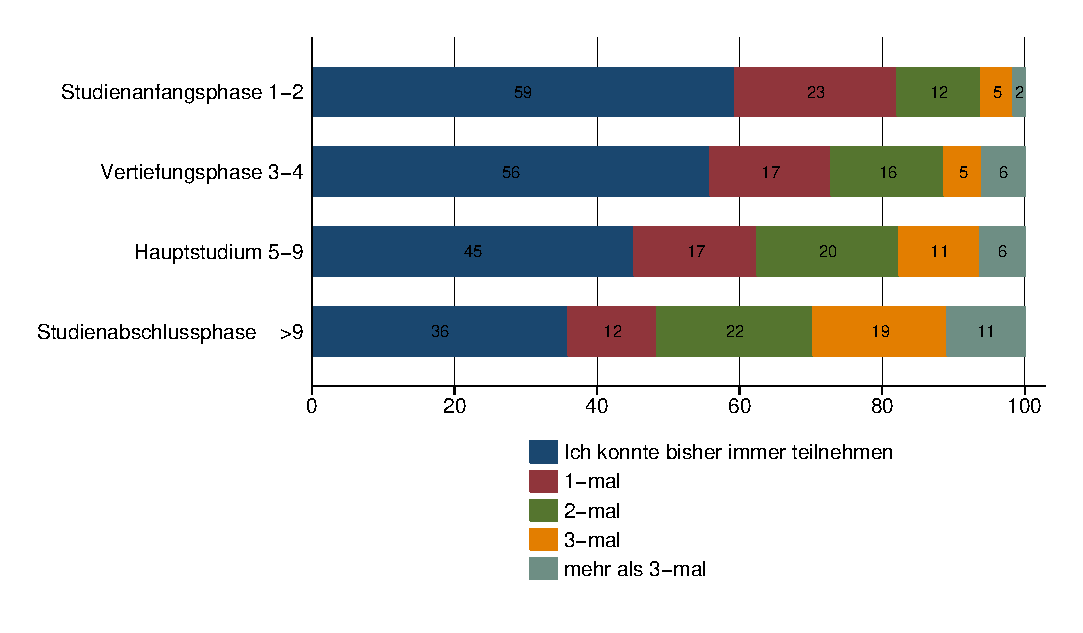
\includegraphics[
%  defaultresolution=72 !,
%  bmpsizefast=false
%]{image}
%\end{verbatim}
% \end{quote}
%
% \subsubsection{Hints}
%
% \begin{itemize}
% \item My version of \xfile{dvips.def} 1999/02/16 v3.0i defines
%       rules for the supported bitmap extensions, but does not
%       include them in the list of extensions that are tried
%       if the file name is not given with an extension.
%       In such a case, the list of extensions can be set
%       by \cs{DeclareGraphicsExtensions}, see \xpackage{grfguide}.
%       The following code just extends the list:
%       \begin{quote}
%\begin{verbatim}
%\makeatletter
%\g@addto@macro\Gin@extensions{,.bmp,.pcx,.msp}
%\makeatother
%\end{verbatim}
%       \end{quote}
% \item My version of \xfile{dvipdfm.def} 1998/11/24 vx.x misses
%       the graphics rule for PNG files. It can be added by:
%       \begin{quote}
%\begin{verbatim}
%\DeclareGraphicsRule{.png}{bmp}{.bb}{#1}
%\end{verbatim}
%       \end{quote}
%       See the previous issue to add the extension \xfile{.png} to the list
%       of extensions for package \xpackage{graphics}.
% \end{itemize}
%
% \subsubsection{Test program}
%
% There is a test program \xfile{bmpsize-test.tex}. Run it through
% \verb|latex|, \verb|pdflatex|, or \verb|pdftex|. Then given
% image files are inspected and the result is printed.
%
% \subsubsection{Interface for programmers}
%
% The macro names of the parsers are \verb|\bmpsize@read@|\meta{type}.
% Example: \cs{bmpsize@read@jpg} in case of JPEG.
%
% A parser sets the switch \cs{ifbmpsize@ok} to true, if it
% could successfully parse the image file.
% The width and height are returnd in \cs{bmpsize@width} and
% \cs{bmpsize@height}. If information about density is available,
% it is used to calculate width and height of the image, otherwise
% the values given by option \xoption{defaultresolution} is used.
% \xoption{resolution} overwrites the values in the image file.
%
% \subsection{Improved bitmap inclusion}
%
% Some drivers for package \xpackage{graphics} define the graphics
% type \xoption{bmp} for bitmap images. The code in the standard
% drivers for \xoption{dvips}, \xoption{dvipdfm}, and \xoption{dvipdfmx}
% is very basic and misses essential features of the
% package \xpackage{graphicx}. Therefore the code for bitmap
% inclusion is automatically rewritten by this package to add
% the following features:
% \begin{itemize}
% \item Support for \xoption{viewport} and \xoption{trim}.
% \item Support for \xoption{clip}.
% \item In case of \xoption{dvipdfm} and \xoption{dvipdfmx} the
%       bitmap images are reused and not included again if they
%       are used more than once.
% \end{itemize}
% However, there is a difference between \xoption{dvipdfm} and
% \xoption{dvipdfmx}, especially if images are reused. In the
% former case the reused box has width and height of 1bp, in the
% latter case its natural width. Thus the correct driver option must be given.
% \xoption{dvipdfm} and \xoption{dvipdfmx} are not equivalent.
%
% Older versions of \xoption{dvipdfmx} uses a size of 1in. However I do
% want to distinguish between versions of the same program. Therefore the
% support of these older versions has stopped with version 1.6 of this package.
% Use version dvipdfmx-20090708 or newer (some few versions before will
% probably also work, but I don't want to investigate this further).
%
% \StopEventually{
% }
%
% \section{Implementation}
%
% \subsection{Basic package \xpackage{bmpsize-base}}
%
%    Identification.
%    \begin{macrocode}
%<*base>
\ProvidesPackage{bmpsize-base}%
  [2009/09/04 v1.6 Basic part of bmpsize (HO)]%
%    \end{macrocode}
%    Modules of package \xpackage{fp} are used for calculations.
%    \begin{macrocode}
\RequirePackage{fp-basic}
\RequirePackage{fp-snap}
%    \end{macrocode}
%    Package \xpackage{fp} uses nested \cs{loop} structures.
%    That breaks with the plain-\TeX\ version of \cs{loop}.
%    Therefore we use the \LaTeX\ variant.
%    \begin{macro}{\@bmpsize@plain@loop}
%    \begin{macrocode}
\long\def\@bmpsize@plain@loop#1\repeat{%
  \def\iterate{%
    #1\relax
    \expandafter\iterate\fi
  }%
  \iterate
  \let\iterate\relax
}
%    \end{macrocode}
%    \end{macro}
%    \begin{macrocode}
\RequirePackage{pdftexcmds}[2007/11/11]
%    \end{macrocode}
%    \begin{macrocode}
\newif\ifbmpsize@ok
\let\@bmpsize@ok\bmpsize@oktrue

\newif\if@bmpsize@bigendian
\newif\if@bmpsize@absnum
\newif\if@bmpsize@user@resolution
\newif\if@bmpsize@fast
\@bmpsize@fasttrue

\def\@bmpsize@init{%
  \let\@bmpsize@org@plain@loop\loop
  \let\loop\@bmpsize@plain@loop
  \bmpsize@okfalse
  \@bmpsize@bigendiantrue
  \@bmpsize@absnumfalse
  \let\bmpsize@pixelwidth\relax
  \let\bmpsize@pixelheight\relax
  \let\bmpsize@pixelx\relax
  \let\bmpsize@pixely\relax
  \let\bmpsize@unit\relax
  \let\bmpsize@pixelxdenom\relax
  \let\bmpsize@pixelydenom\relax
  \let\bmpsize@orientation\relax
}

\def\@bmpsize@stop#1\@nil{}

\def\@bmpsize@loop#1{%
  #1%
  \@bmpsize@loop{#1}%
}
\def\@bmpsize@break#1\@bmpsize@loop#2{}

\def\@bmpsize@size#1#2#3{%
  \edef#3{\pdf@filesize{#1}}%
  \ifx#3\@empty
    \expandafter\@bmpsize@stop
  \fi
  \ifnum#3<#2\relax
    \expandafter\@bmpsize@stop
  \fi
}

\def\@bmpsize@read#1#2#3{%
  \edef\@bmpsize@buf{\pdf@filedump{#3}{#2}{#1}}%
  \edef\@bmpsize@temp{%
    \noexpand\@bmpsize@check@byte{#2}\@bmpsize@buf{}{}\noexpand\\%
  }%
  \@bmpsize@temp
}
\def\@bmpsize@fillbuf#1{%
  \ifx\@bmpsize@buf\@empty
    \expandafter\@firstofone
  \else
    \expandafter\@gobble
  \fi
  {%
    \edef\@bmpsize@buf{%
      \pdf@filedump{\bmpsize@offset}{\bmpsize@fillbuflength}{#1}%
    }%
    \ifx\@bmpsize@buf\@empty
      \expandafter\@bmpsize@stop
    \fi
    \edef\bmpsize@offset{\the\numexpr\bmpsize@offset+\bmpsize@fillbuflength}%
  }%
}
\def\bmpsize@fillbuflength{10}

\def\@bmpsize@append#1#2#3{%
  \edef#1{#2#3}%
}
\def\@bmpsize@pushback#1{%
  \edef\@bmpsize@buf{#1\@bmpsize@buf}%
}

\def\@bmpsize@iswhite#1{%
  \ifnum\pdf@strcmp{#1}{09}=\z@
  \else
    \ifnum\pdf@strcmp{#1}{0A}=\z@
    \else
      \ifnum\pdf@strcmp{#1}{0D}=\z@
      \else
        \ifnum\pdf@strcmp{#1}{20}=\z@
        \else
          1%
        \fi
      \fi
    \fi
  \fi
  \space
}
\def\@bmpsize@isdigit#1{%
  \ifnum\pdf@strcmp{#1}{30}<\z@
    1%
  \else
    \ifnum\pdf@strcmp{#1}{39}>\z@
      1%
    \fi
  \fi
  \space
}

\def\@bmpsize@check@byte#1#2#3{%
  \ifnum#1<\@ne
    \csname fi\endcsname
    \@bmpsize@cleanup@end
  \else
    \csname fi\endcsname
  \ifx!#2#3!%
    \csname fi\endcsname
    \@bmpsize@stop
  \else
    \csname fi\endcsname
    \expandafter\@bmpsize@check@byte\expandafter{\the\numexpr#1-1}%
}
\def\@bmpsize@cleanup@end#1\\{}

\def\@bmpsize@swap@maybe#1{%
  \if@bmpsize@bigendian
  \else
    \edef#1{\expandafter\@bmpsize@@swap#1\@empty\@empty\@empty\@empty}%
  \fi
}
\def\@bmpsize@@swap#1#2#3#4#5#6#7#8{%
  #7#8#5#6#3#4#1#2%
}

\def\@bmpsize@skip@one{%
  \edef\@bmpsize@buf{\expandafter\@gobbletwo\@bmpsize@buf}%
}
\def\@bmpsize@skip@two{%
  \edef\@bmpsize@buf{\expandafter\@gobblefour\@bmpsize@buf}%
}
\def\@bmpsize@skip@four{%
  \edef\@bmpsize@buf{%
    \expandafter\expandafter\expandafter\@gobblefour\expandafter
    \@gobblefour\@bmpsize@buf
  }%
}

\def\@bmpsize@grab#1#2{%
  \edef#1{\noexpand\@bmpsize@grab@byte#2=\@bmpsize@buf\noexpand\\}%
  \edef#1{#1}%
}
\def\@bmpsize@grab@byte#1=#2#3{%
  #2#3%
  \ifnum#1>\@ne
    \expandafter\@bmpsize@grab@byte\the\numexpr#1-1\expandafter=%
  \else
    \expandafter\@bmpsize@cleanup@end
  \fi
}

\def\@bmpsize@abs@maybe#1{%
  \let\@bmpsize@temp\relax
  \if@bmpsize@absnum
    \ifnum"\expandafter\@car#1\@nil>7 %
      \edef#1{\expandafter\@bmpsize@abs@byte#1\relax}%
      \ifnum\pdf@strcmp{#1}{7FFFFFFF}=\z@
        \let\@bmpsize@temp\@bmpsize@stop
      \else
        \def\@bmpsize@temp{\edef#1{\the\numexpr#1+1}}%
      \fi
    \fi
  \fi
}
\def\@bmpsize@abs@byte#1{%
  \ifx#1\relax
  \else
    \ifcase"0#1 %
      F\or E\or D\or C\or B\or A\or 9\or 8\or
      7\or 6\or 5\or 4\or 3\or 2\or 1\or 0%
    \fi
    \expandafter\@bmpsize@abs@byte
  \fi
}

\def\@bmpsize@num@one#1{%
  \@bmpsize@grab#11%
  \@bmpsize@abs@maybe#1%
  \edef#1{\number"#1}%
  \@bmpsize@temp
  \@bmpsize@skip@one
}
\def\@bmpsize@num@two#1{%
  \@bmpsize@grab#12%
  \@bmpsize@swap@maybe#1%
  \@bmpsize@abs@maybe#1%
  \edef#1{\number"#1}%
  \@bmpsize@temp
  \@bmpsize@skip@two
}
\def\@bmpsize@num@four#1{%
  \@bmpsize@grab#14%
  \@bmpsize@swap@maybe#1%
  \@bmpsize@abs@maybe#1%
  \ifnum\pdf@strcmp{#1}{7FFFFFFF}>\z@
    \expandafter\@bmpsize@stop
  \fi
  \edef#1{\number"#1}%
  \@bmpsize@temp
  \@bmpsize@skip@four
}

\def\@bmpsize@div#1#2#3{% #1 := #2/#3
  \FPdiv#1{#2}{#3}%
  \@bmpsize@beautify#1%
}
\def\@bmpsize@beautify#1{%
  \FPifint#1%
    \edef#1{\expandafter\@bmpsize@trunc#1.\@nil}%
  \else
    \edef#1{\expandafter\@bmpsize@cleanup@frac#1.\@nil}%
  \fi
}
\def\@bmpsize@trunc#1.#2\@nil{#1}
% #1 isn't an integer, thus we should have at least one
% necessary digit after the dot
\def\@bmpsize@cleanup@frac#1.#2#3.#4\@nil{%
  #1.#2%
  \ifx\\#3\\%
  \else
    \@bmpsize@cleanup@fracdigits#3000000000\@nil
  \fi
}
\def\@bmpsize@cleanup@fracdigits#1#2#3#4#5#6#7#8#9{%
  \ifcase#9 %
    \ifcase#8 %
      \ifcase#7 %
        \ifcase#6 %
          \ifcase#5 %
            \ifcase #4 %
              \ifcase #3 %
                \ifcase #2 %
                  \ifcase #1 %
                  \else
                    #1%
                  \fi
                \else
                  #1#2%
                \fi
              \else
                #1#2#3%
              \fi
            \else
              #1#2#3#4%
            \fi
          \else
            #1#2#3#4#5%
          \fi
        \else
          #1#2#3#4#5#6%
        \fi
      \else
        #1#2#3#4#5#6#7%
      \fi
    \else
      #1#2#3#4#5#6#7#8%
    \fi
  \else
    #1#2#3#4#5#6#7#8#9%
  \fi
  \@bmpsize@trunc.%
}

\def\@bmpsize@end{%
  \ifbmpsize@ok
    \ifx\bmpsize@pixelwidth\relax
      \bmpsize@okfalse
    \fi
    \ifx\bmpsize@pixelheight\relax
      \bmpsize@okfalse
    \fi
  \fi
  \ifbmpsize@ok
    \ifnum\bmpsize@pixelwidth>\z@
    \else
      \bmpsize@okfalse
    \fi
    \ifnum\bmpsize@pixelheight>\z@
    \else
      \bmpsize@okfalse
    \fi
  \fi
  \ifbmpsize@ok
    \ifcase 0%
      \ifx\bmpsize@pixelx\relax 1 \fi
      \ifx\bmpsize@pixely\relax 1 \fi
      \ifnum\bmpsize@pixelx>\z@\else 1 \fi
      \ifnum\bmpsize@pixely>\z@\else 1 \fi
      \ifx\bmpsize@pixelxdenom\relax
         \ifx\bmpsize@pixelydenom\relax\else 1 \fi
      \else
        \ifnum\bmpsize@pixelxdenom>\z@\else 1 \fi
      \fi
      \ifx\bmpsize@pixelydenom\relax
      \else
        \ifnum\bmpsize@pixelydenom>\z@\else 1 \fi
      \fi
    \else
      \let\bmpsize@pixelx\relax
      \let\bmpsize@pixely\relax
      \let\bmpsize@unit\relax
      \let\bmpsize@pixelxdenom\relax
      \let\bmpsize@pixelydenom\relax
    \fi
    \ifx\bmpsize@pixelxdenom\relax
    \else
      \@bmpsize@div\bmpsize@pixelx\bmpsize@pixelx\bmpsize@pixelxdenom
      \@bmpsize@div\bmpsize@pixely\bmpsize@pixely\bmpsize@pixelydenom
      \let\bmpsize@pixelxdenom\relax
      \let\bmpsize@pixelydenom\relax
    \fi
    \ifcase 0\ifx\bmpsize@unit\relax 1\fi
             \if@bmpsize@user@resolution 1\fi
             \relax
      \let\bmpsize@calc@unit\bmpsize@unit
      \let\bmpsize@calc@pixelx\bmpsize@pixelx
      \let\bmpsize@calc@pixely\bmpsize@pixely
    \else
      \let\bmpsize@calc@unit\bmpsize@unit@default
      \let\bmpsize@calc@pixelx\bmpsize@pixelx@default
      \let\bmpsize@calc@pixely\bmpsize@pixely@default
      \ifx\bmpsize@calc@pixely\Gin@exclamation
        \ifx\bmpsize@pixelx\relax
          \let\bmpsize@calc@pixely\bmpsize@calc@pixelx
        \else
          \FPdiv\bmpsize@calc@pixely\bmpsize@calc@pixelx\bmpsize@pixelx
          \FPmul\bmpsize@calc@pixely\bmpsize@calc@pixely\bmpsize@pixely
        \fi
      \else
        \ifx\bmpsize@calc@pixelx\Gin@exclamation
          \ifx\bmpsize@pixelx\relax
            \let\bmpsize@calc@pixelx\bmpsize@calc@pixely
          \else
            \FPdiv\bmpsize@calc@pixelx\bmpsize@calc@pixely\bmpsize@pixely
            \FPmul\bmpsize@calc@pixelx\bmpsize@calc@pixelx\bmpsize@pixelx
          \fi
        \fi
      \fi
    \fi
    \FPdiv\bmpsize@width\bmpsize@pixelwidth\bmpsize@calc@pixelx
    \FPdiv\bmpsize@height\bmpsize@pixelheight\bmpsize@calc@pixely
    % calculation of width and height in bp for package graphics
    % 1in = 72bp = 72.27pt, 72/72.27 = 8/8.03, 1pt = 65536sp
    \if@bmpsize@fast
      \edef\bmpsize@width{%
        \strip@pt\dimexpr.99626\dimexpr
        \bmpsize@width\dimexpr\bmpsize@calc@unit
      }%
      \edef\bmpsize@height{%
        \strip@pt\dimexpr.99626\dimexpr
        \bmpsize@height\dimexpr\bmpsize@calc@unit
      }%
    \else
      \edef\@bmpsize@temp{\number\dimexpr\bmpsize@calc@unit}%
      \ifnum\@bmpsize@temp>100000 %
        \FPmul\@bmpsize@temp\@bmpsize@temp{0.00001}%
        \def\@bmpsize@corr{100000}%
      \else
        \let\@bmpsize@corr\relax
      \fi
      \FPmul\bmpsize@width\bmpsize@width\@bmpsize@temp
      \FPmul\bmpsize@height\bmpsize@height\@bmpsize@temp
      \FPmul\bmpsize@width\bmpsize@width{8}%
      \FPmul\bmpsize@height\bmpsize@height{8}%
      \FPdiv\bmpsize@width\bmpsize@width{8.03}%
      \FPdiv\bmpsize@height\bmpsize@height{8.03}%
      \FPdiv\bmpsize@width\bmpsize@width{65536}%
      \FPdiv\bmpsize@height\bmpsize@height{65536}%
      \ifx\@bmpsize@corr\relax
      \else
        \FPmul\bmpsize@width\bmpsize@width\@bmpsize@corr
        \FPmul\bmpsize@height\bmpsize@height\@bmpsize@corr
      \fi
      \FPround\bmpsize@width\bmpsize@width{5}%
      \FPround\bmpsize@height\bmpsize@height{5}%
      \@bmpsize@beautify\bmpsize@width
      \@bmpsize@beautify\bmpsize@height
    \fi
  \fi
  \let\loop\@bmpsize@org@plain@loop
}
\def\bmpsize@unit@default{72.27pt}% more accurate than 1in
\def\bmpsize@pixelx@default{72}
\let\bmpsize@pixely@default\Gin@exclamation

\def\bmpsize@types{png,jpg,bmp,gif,tiff,pnm,pam,xpm,tga,pcx,msp,sgi}
%</base>
%    \end{macrocode}
%
% \subsection{Bitmap formats}
%
% \subsubsection{png}
%
%\iffalse
%<*ignore>
%\fi
%\begin{verbatim}
%begin png
%big-endian
%
%read 24 0
%grab 8        -> $temp
%check streq $temp [0x89 "PNG" 0x0D 0x0A 0x1A 0x0A]
%num 4         -> $length
%grab 4        -> $temp
%check streq $temp ["IHDR"]
%num 4         -> $pixelwidth
%num 4         -> $pixelheight
%ok
%assign numexpr(20 + $length) -> $offset
%loop
%  read 8 $offset
%  num 4       -> $length
%  grab 4      -> $temp
%  if streq $temp ["IDAT"]
%    stop
%  fi
%  if streq $temp ["pHYs"]
%    read 9 numexpr($offset + 8)
%    num 4     -> $pixelx
%    num 4     -> $pixely
%    grab 1     -> $temp
%    if numeq $temp 1
%      assign {100cm} -> $unit
%    fi
%    stop
%  fi
%  assign numexpr($offset + 12 + $length) -> $offset
%repeat
%end
%\end{verbatim}
%\iffalse
%</ignore>
%\fi
%    \begin{macro}{\bmpsize@read@png}
%    \begin{macrocode}
%<*base>
\def\bmpsize@read@png#1{%
  \@bmpsize@init
  \@bmpsize@bigendiantrue
  \@bmpsize@read{#1}{24}{0}%
  \@bmpsize@grab\bmpsize@temp{8}%
  \@bmpsize@skip@four
  \@bmpsize@skip@four
  \ifnum\pdf@strcmp{\bmpsize@temp}{89504E470D0A1A0A}=\z@
  \else
    \expandafter\@bmpsize@stop
  \fi
  \@bmpsize@num@four\bmpsize@length
  \@bmpsize@grab\bmpsize@temp{4}%
  \@bmpsize@skip@four
  \ifnum\pdf@strcmp{\bmpsize@temp}{49484452}=\z@
  \else
    \expandafter\@bmpsize@stop
  \fi
  \@bmpsize@num@four\bmpsize@pixelwidth
  \@bmpsize@num@four\bmpsize@pixelheight
  \@bmpsize@ok
  \edef\bmpsize@offset{\the\numexpr20+\bmpsize@length}%
  \@bmpsize@loop{%
    \@bmpsize@read{#1}{8}{\bmpsize@offset}%
    \@bmpsize@num@four\bmpsize@length
    \@bmpsize@grab\bmpsize@temp{4}%
    \@bmpsize@skip@four
    \ifnum\pdf@strcmp{\bmpsize@temp}{49444154}=\z@
      \expandafter\@firstofone
    \else
      \expandafter\@gobble
    \fi
    {%
      \@bmpsize@stop
    }%
    \ifnum\pdf@strcmp{\bmpsize@temp}{70485973}=\z@
      \expandafter\@firstofone
    \else
      \expandafter\@gobble
    \fi
    {%
      \@bmpsize@read{#1}{9}{\numexpr\bmpsize@offset+8\relax}%
      \@bmpsize@num@four\bmpsize@pixelx
      \@bmpsize@num@four\bmpsize@pixely
      \@bmpsize@grab\bmpsize@temp{1}%
      \@bmpsize@skip@one
      \ifnum\bmpsize@temp=1\relax
        \expandafter\@firstofone
      \else
        \expandafter\@gobble
      \fi
      {%
        \def\bmpsize@unit{100cm}%
      }%
      \@bmpsize@stop
    }%
    \edef\bmpsize@offset{\the\numexpr\bmpsize@offset+12+\bmpsize@length}%
  }%
  \@bmpsize@stop
  \@nil
  \@bmpsize@end
}%
%</base>
%    \end{macrocode}
%    \end{macro}
%
% \subsubsection{jpg}
%
%\iffalse
%<*ignore>
%\fi
%\begin{verbatim}
%begin jpg
%
%read 3 0
%grab 3      -> $temp % SOI and 0xFF
%check streq $temp [0xFF 0xD8 0xFF]
%assign {2} -> $offset
%assign {0} -> $exifdensity
%loop
%  read 4 $offset
%  grab 1    -> $temp
%  check streq $temp [0xFF]
%  num 1    -> $temp
%  if numeq $temp 0xDA % SOS
%    stop
%  fi
%  % look for JFIF APP0 segment
%  if numeq $temp 0xE0 % APP0
%    num 2       -> $length
%    if numeq $exifdensity 0
%      if numge $length 16 % a JFIF segment has 16 bytes at least
%        read 12 numexpr($offset + 4)
%        grab 5      -> $temp % identifier
%        if streq $temp ["JFIF" 0x0]
%          check numge $length 16
%          skip 2 % version
%          num 1       -> $temp % units
%          if numeq $temp 1
%            assign {72.27pt} -> $unit
%          else
%            if numeq $temp 2
%              assign {1cm} -> $unit
%            fi
%          fi
%          num 2    -> $pixelx
%          num 2    -> $pixely
%        fi
%      fi
%    fi
%  else
%    if numeq $temp 0xE1 % APP1
%      % look for Exif APP1 segment
%      num 2 -> $length
%      if numge $length 20 % identifier (6) + Tiff header (8) + first IFD (>=6)
%        read 20 numexpr($offset + 4)
%        grab 6 -> $temp
%        if streq $temp ["Exif" 0x0 0x0]
%          assign numexpr($offset + 10) -> $exifoffset
%          % read TIFF header
%          grab 2 -> $temp
%          if streq $temp ["II"]
%            little-endian
%          else
%            check streq $temp ["MM"]
%            % big-endian
%          fi
%          num 2 -> $temp
%          check numeq $temp 42
%          num 4 -> $temp % offset of first IFD
%          check numgt $temp 0
%          % read first IFD
%          assign numexpr($temp + $exifoffset) -> $off
%          read 2 $off
%          num 2 -> $entries
%          assign numexpr($off + 2) -> $off
%          loop
%            if numeq $entries 0
%              break
%            fi
%            assign numexpr($entries - 1) -> $entries
%            % entry format:
%            % 2 tag
%            % 2 field type
%            % 4 count
%            % 4 value/offset
%            read 12 $off
%            assign numexpr($off + 12) -> $off
%            num 2 -> $tag
%            if numeq $tag 296 % ResolutionUnit
%              skip 6 % type: 3 (short), count: 1
%              num 2 -> $temp
%              ifcase $temp
%              or % 1
%                clear $unit
%              or % 2
%                assign {72.27pt} -> $unit
%              or % 3
%                assign {1cm} -> $unit
%              else
%                clear $unit % unknown
%              fi
%              ifcase $temp
%              or % 1
%              or % 2
%                assign {1} -> $exifdensity
%              or % 3
%                assign {1} -> $exifdensity
%              else
%                assign $exifdensity -> $exifdensity
%              fi
%            fi
%            % 256 ImageWidth (use width of JPG part)
%            % 257 ImageHeight (use height of JPG part)
%            if numeq $tag 274 % Orientation
%              skip 6 % type: 3 (short), count: 1
%              num 2 -> $temp
%              if numge $temp 0 
%                if numle $temp 8
%                  assign $temp -> $orientation
%                fi
%              fi
%            fi
%            if numeq $tag 282 % XResolution
%              skip 6
%              num 4 -> $temp
%              read 8 numexpr($temp + $exifoffset)
%              num 4 -> $pixelx
%              num 4 -> $temp
%              if numeq $temp 1
%              else
%                assign numexpr($temp) -> $pixelxdenom
%                % div $pixelx $temp -> $pixelx
%              fi
%            fi
%            if numeq $tag 283 % YResolution
%              skip 6
%              num 4 -> $temp
%              read 8 numexpr($temp + $exifoffset)
%              num 4 -> $pixely
%              num 4 -> $temp
%              if numeq $temp 1
%              else
%                assign numexpr($temp) -> $pixelydenom
%                % div $pixely $temp -> $pixely
%              fi
%            fi
%          repeat
%          big-endian
%        fi
%      fi
%    else
%      assign numexpr($temp - 0xC0) -> $temp
%      ifcase $temp % SOF_0
%      or % SOF_1
%      or % SOF_2
%      or % SOF_3
%      or % DHT
%        assign {-1} -> $temp
%      or % SOF_5
%      or % SOF_6
%      or % SOF_7
%      or % JPG
%        assign {-1} -> $temp
%      or % SOF_9
%      or % SOF_10
%      or % SOF_11
%      or % DAC
%        assign {-1} -> $temp
%      or % SOF_13
%      or % SOF_14
%      or % SOF_15
%      else
%        assign {-1} -> $temp
%      fi
%      if numeq $temp -1
%      else
%        read 4 numexpr($offset + 5)
%        num 2  -> $pixelheight
%        num 2  -> $pixelwidth
%        if numeq $pixelheight 0
%          clear $pixelheight
%          stop
%        fi
%        ok
%        stop
%      fi
%      num 2 -> $length
%    fi
%  fi
%  assign numexpr($offset + $length + 2) -> $offset
%repeat
%end
%\end{verbatim}
%\iffalse
%</ignore>
%\fi
%    \begin{macro}{\bmpsize@read@jpg}
%    \begin{macrocode}
%<*base>
\def\bmpsize@read@jpg#1{%
  \@bmpsize@init
  \@bmpsize@read{#1}{3}{0}%
  \@bmpsize@grab\bmpsize@temp{3}%
  \@bmpsize@skip@two
  \@bmpsize@skip@one
  \ifnum\pdf@strcmp{\bmpsize@temp}{FFD8FF}=\z@
  \else
    \expandafter\@bmpsize@stop
  \fi
  \def\bmpsize@offset{2}%
  \def\bmpsize@exifdensity{0}%
  \@bmpsize@loop{%
    \@bmpsize@read{#1}{4}{\bmpsize@offset}%
    \@bmpsize@grab\bmpsize@temp{1}%
    \@bmpsize@skip@one
    \ifnum\pdf@strcmp{\bmpsize@temp}{FF}=\z@
    \else
      \expandafter\@bmpsize@stop
    \fi
    \@bmpsize@num@one\bmpsize@temp
    \ifnum\bmpsize@temp=218\relax
      \expandafter\@firstofone
    \else
      \expandafter\@gobble
    \fi
    {%
      \@bmpsize@stop
    }%
    \ifnum\bmpsize@temp=224\relax
      \expandafter\@firstoftwo
    \else
      \expandafter\@secondoftwo
    \fi
    {%
      \@bmpsize@num@two\bmpsize@length
      \ifnum\bmpsize@exifdensity=0\relax
        \expandafter\@firstofone
      \else
        \expandafter\@gobble
      \fi
      {%
        \unless\ifnum\bmpsize@length<16\relax
          \expandafter\@firstofone
        \else
          \expandafter\@gobble
        \fi
        {%
          \@bmpsize@read{#1}{12}{\numexpr\bmpsize@offset+4\relax}%
          \@bmpsize@grab\bmpsize@temp{5}%
          \@bmpsize@skip@four
          \@bmpsize@skip@one
          \ifnum\pdf@strcmp{\bmpsize@temp}{4A46494600}=\z@
            \expandafter\@firstofone
          \else
            \expandafter\@gobble
          \fi
          {%
            \ifnum\bmpsize@length<16\relax
              \expandafter\@bmpsize@stop
            \fi
            \@bmpsize@skip@two
            \@bmpsize@num@one\bmpsize@temp
            \ifnum\bmpsize@temp=1\relax
              \expandafter\@firstoftwo
            \else
              \expandafter\@secondoftwo
            \fi
            {%
              \def\bmpsize@unit{72.27pt}%
            }{%
              \ifnum\bmpsize@temp=2\relax
                \expandafter\@firstofone
              \else
                \expandafter\@gobble
              \fi
              {%
                \def\bmpsize@unit{1cm}%
              }%
            }%
            \@bmpsize@num@two\bmpsize@pixelx
            \@bmpsize@num@two\bmpsize@pixely
          }%
        }%
      }%
    }{%
      \ifnum\bmpsize@temp=225\relax
        \expandafter\@firstoftwo
      \else
        \expandafter\@secondoftwo
      \fi
      {%
        \@bmpsize@num@two\bmpsize@length
        \unless\ifnum\bmpsize@length<20\relax
          \expandafter\@firstofone
        \else
          \expandafter\@gobble
        \fi
        {%
          \@bmpsize@read{#1}{20}{\numexpr\bmpsize@offset+4\relax}%
          \@bmpsize@grab\bmpsize@temp{6}%
          \@bmpsize@skip@four
          \@bmpsize@skip@two
          \ifnum\pdf@strcmp{\bmpsize@temp}{457869660000}=\z@
            \expandafter\@firstofone
          \else
            \expandafter\@gobble
          \fi
          {%
            \edef\bmpsize@exifoffset{\the\numexpr\bmpsize@offset+10}%
            \@bmpsize@grab\bmpsize@temp{2}%
            \@bmpsize@skip@two
            \ifnum\pdf@strcmp{\bmpsize@temp}{4949}=\z@
              \expandafter\@firstoftwo
            \else
              \expandafter\@secondoftwo
            \fi
            {%
              \@bmpsize@bigendianfalse
            }{%
              \ifnum\pdf@strcmp{\bmpsize@temp}{4D4D}=\z@
              \else
                \expandafter\@bmpsize@stop
              \fi
            }%
            \@bmpsize@num@two\bmpsize@temp
            \ifnum\bmpsize@temp=42\relax
            \else
              \expandafter\@bmpsize@stop
            \fi
            \@bmpsize@num@four\bmpsize@temp
            \ifnum\bmpsize@temp>0\relax
            \else
              \expandafter\@bmpsize@stop
            \fi
            \edef\bmpsize@off{\the\numexpr\bmpsize@temp+\bmpsize@exifoffset}%
            \@bmpsize@read{#1}{2}{\bmpsize@off}%
            \@bmpsize@num@two\bmpsize@entries
            \edef\bmpsize@off{\the\numexpr\bmpsize@off+2}%
            \@bmpsize@loop{%
              \ifnum\bmpsize@entries=0\relax
                \expandafter\@firstofone
              \else
                \expandafter\@gobble
              \fi
              {%
                \@bmpsize@break
              }%
              \edef\bmpsize@entries{\the\numexpr\bmpsize@entries-1}%
              \@bmpsize@read{#1}{12}{\bmpsize@off}%
              \edef\bmpsize@off{\the\numexpr\bmpsize@off+12}%
              \@bmpsize@num@two\bmpsize@tag
              \ifnum\bmpsize@tag=296\relax
                \expandafter\@firstofone
              \else
                \expandafter\@gobble
              \fi
              {%
                \@bmpsize@skip@four
                \@bmpsize@skip@two
                \@bmpsize@num@two\bmpsize@temp
                \ifcase\bmpsize@temp\relax
                \or
                  \let\bmpsize@unit\relax
                \or
                  \def\bmpsize@unit{72.27pt}%
                \or
                  \def\bmpsize@unit{1cm}%
                \else
                  \let\bmpsize@unit\relax
                \fi
                \ifcase\bmpsize@temp\relax
                \or
                \or
                  \def\bmpsize@exifdensity{1}%
                \or
                  \def\bmpsize@exifdensity{1}%
                \else
                  \let\bmpsize@exifdensity\bmpsize@exifdensity
                \fi
              }%
              \ifnum\bmpsize@tag=274\relax
                \expandafter\@firstofone
              \else
                \expandafter\@gobble
              \fi
              {%
                \@bmpsize@skip@four
                \@bmpsize@skip@two
                \@bmpsize@num@two\bmpsize@temp
                \unless\ifnum\bmpsize@temp<0\relax
                  \expandafter\@firstofone
                \else
                  \expandafter\@gobble
                \fi
                {%
                  \unless\ifnum\bmpsize@temp>8\relax
                    \expandafter\@firstofone
                  \else
                    \expandafter\@gobble
                  \fi
                  {%
                    \let\bmpsize@orientation\bmpsize@temp
                  }%
                }%
              }%
              \ifnum\bmpsize@tag=282\relax
                \expandafter\@firstofone
              \else
                \expandafter\@gobble
              \fi
              {%
                \@bmpsize@skip@four
                \@bmpsize@skip@two
                \@bmpsize@num@four\bmpsize@temp
                \@bmpsize@read{#1}{8}{\numexpr\bmpsize@temp+\bmpsize@exifoffset\relax}%
                \@bmpsize@num@four\bmpsize@pixelx
                \@bmpsize@num@four\bmpsize@temp
                \ifnum\bmpsize@temp=1\relax
                  \expandafter\@gobble
                \else
                  \expandafter\@firstofone
                \fi
                {%
                  \edef\bmpsize@pixelxdenom{\the\numexpr\bmpsize@temp}%
                }%
              }%
              \ifnum\bmpsize@tag=283\relax
                \expandafter\@firstofone
              \else
                \expandafter\@gobble
              \fi
              {%
                \@bmpsize@skip@four
                \@bmpsize@skip@two
                \@bmpsize@num@four\bmpsize@temp
                \@bmpsize@read{#1}{8}{\numexpr\bmpsize@temp+\bmpsize@exifoffset\relax}%
                \@bmpsize@num@four\bmpsize@pixely
                \@bmpsize@num@four\bmpsize@temp
                \ifnum\bmpsize@temp=1\relax
                  \expandafter\@gobble
                \else
                  \expandafter\@firstofone
                \fi
                {%
                  \edef\bmpsize@pixelydenom{\the\numexpr\bmpsize@temp}%
                }%
              }%
            }%
            \@bmpsize@bigendiantrue
          }%
        }%
      }{%
        \edef\bmpsize@temp{\the\numexpr\bmpsize@temp-192}%
        \ifcase\bmpsize@temp\relax
        \or
        \or
        \or
        \or
          \def\bmpsize@temp{-1}%
        \or
        \or
        \or
        \or
          \def\bmpsize@temp{-1}%
        \or
        \or
        \or
        \or
          \def\bmpsize@temp{-1}%
        \or
        \or
        \or
        \else
          \def\bmpsize@temp{-1}%
        \fi
        \ifnum\bmpsize@temp=-1\relax
          \expandafter\@gobble
        \else
          \expandafter\@firstofone
        \fi
        {%
          \@bmpsize@read{#1}{4}{\numexpr\bmpsize@offset+5\relax}%
          \@bmpsize@num@two\bmpsize@pixelheight
          \@bmpsize@num@two\bmpsize@pixelwidth
          \ifnum\bmpsize@pixelheight=0\relax
            \expandafter\@firstofone
          \else
            \expandafter\@gobble
          \fi
          {%
            \let\bmpsize@pixelheight\relax
            \@bmpsize@stop
          }%
          \@bmpsize@ok
          \@bmpsize@stop
        }%
        \@bmpsize@num@two\bmpsize@length
      }%
    }%
    \edef\bmpsize@offset{\the\numexpr\bmpsize@offset+\bmpsize@length+2}%
  }%
  \@bmpsize@stop
  \@nil
  \@bmpsize@end
}%
%</base>
%    \end{macrocode}
%    \end{macro}
%
% \subsubsection{bmp}
%
%\iffalse
%<*ignore>
%\fi
%\begin{verbatim}
%begin bmp
%little-endian
%
%read 26 0
%grab 2 -> $temp
%check streq $temp ["BM"]
%skip 12
%% header size is 4 bytes in V3+, unknown for V1, V2,
%% known header sizes fit in 2 bytes
%num 2   -> $temp
%if numeq $temp 12 % V1
%  skip 2
%  num 2 -> $pixelwidth
%  num 2 -> $pixelheight
%  % no resolution entries
%  ok
%  stop
%fi
%if numeq $temp 64 % V2
%  skip 2
%  num 2 -> $pixelwidth
%  num 2 -> $pixelheight
%  % missing specification for resolution
%  ok
%  stop
%fi
%% V3, V4, V5
%skip 2
%num 4 -> $pixelwidth
%absnum 4 -> $pixelheight
%ok
%read 8 38
%num 4 -> $pixelx
%num 4 -> $pixely
%assign {100cm} -> $unit
%end
%\end{verbatim}
%\iffalse
%</ignore>
%\fi
%    \begin{macro}{\bmpsize@read@bmp}
%    \begin{macrocode}
%<*base>
\def\bmpsize@read@bmp#1{%
  \@bmpsize@init
  \@bmpsize@bigendianfalse
  \@bmpsize@read{#1}{26}{0}%
  \@bmpsize@grab\bmpsize@temp{2}%
  \@bmpsize@skip@two
  \ifnum\pdf@strcmp{\bmpsize@temp}{424D}=\z@
  \else
    \expandafter\@bmpsize@stop
  \fi
  \@bmpsize@skip@four
  \@bmpsize@skip@four
  \@bmpsize@skip@four
  \@bmpsize@num@two\bmpsize@temp
  \ifnum\bmpsize@temp=12\relax
    \expandafter\@firstofone
  \else
    \expandafter\@gobble
  \fi
  {%
    \@bmpsize@skip@two
    \@bmpsize@num@two\bmpsize@pixelwidth
    \@bmpsize@num@two\bmpsize@pixelheight
    \@bmpsize@ok
    \@bmpsize@stop
  }%
  \ifnum\bmpsize@temp=64\relax
    \expandafter\@firstofone
  \else
    \expandafter\@gobble
  \fi
  {%
    \@bmpsize@skip@two
    \@bmpsize@num@two\bmpsize@pixelwidth
    \@bmpsize@num@two\bmpsize@pixelheight
    \@bmpsize@ok
    \@bmpsize@stop
  }%
  \@bmpsize@skip@two
  \@bmpsize@num@four\bmpsize@pixelwidth
  \@bmpsize@absnumtrue
  \@bmpsize@num@four\bmpsize@pixelheight
  \@bmpsize@absnumfalse
  \@bmpsize@ok
  \@bmpsize@read{#1}{8}{38}%
  \@bmpsize@num@four\bmpsize@pixelx
  \@bmpsize@num@four\bmpsize@pixely
  \def\bmpsize@unit{100cm}%
  \@bmpsize@stop
  \@nil
  \@bmpsize@end
}%
%</base>
%    \end{macrocode}
%    \end{macro}
%
% \subsubsection{gif}
%
%\iffalse
%<*ignore>
%\fi
%\begin{verbatim}
%begin gif
%little-endian
%
%% Header
%read 13 0
%grab 3      -> $temp
%check streq $temp ["GIF"]
%skip 3      % version
%
%% Logical Screen Descriptor
%num 2       -> $pixelwidth
%num 2       -> $pixelheight
%skip 2
%num 1       -> $temp % Pixel Aspect Ratio
%if numeq $temp 0
%else
%  assign numexpr($temp + 15) -> $pixelx
%  assign {64}     -> $pixely
%fi
%ok
%end
%\end{verbatim}
%\iffalse
%</ignore>
%\fi
%    \begin{macro}{\bmpsize@read@gif}
%    \begin{macrocode}
%<*base>
\def\bmpsize@read@gif#1{%
  \@bmpsize@init
  \@bmpsize@bigendianfalse
  \@bmpsize@read{#1}{13}{0}%
  \@bmpsize@grab\bmpsize@temp{3}%
  \@bmpsize@skip@two
  \@bmpsize@skip@one
  \ifnum\pdf@strcmp{\bmpsize@temp}{474946}=\z@
  \else
    \expandafter\@bmpsize@stop
  \fi
  \@bmpsize@skip@two
  \@bmpsize@skip@one
  \@bmpsize@num@two\bmpsize@pixelwidth
  \@bmpsize@num@two\bmpsize@pixelheight
  \@bmpsize@skip@two
  \@bmpsize@num@one\bmpsize@temp
  \ifnum\bmpsize@temp=0\relax
    \expandafter\@gobble
  \else
    \expandafter\@firstofone
  \fi
  {%
    \edef\bmpsize@pixelx{\the\numexpr\bmpsize@temp+15}%
    \def\bmpsize@pixely{64}%
  }%
  \@bmpsize@ok
  \@bmpsize@stop
  \@nil
  \@bmpsize@end
}%
%</base>
%    \end{macrocode}
%    \end{macro}
%
% \subsubsection{tiff}
%
%\iffalse
%<*ignore>
%\fi
%\begin{verbatim}
%begin tiff
%% defaults
%assign {72.27pt} -> $unit
%
%% Image File Header
%read 8 0
%grab 2 -> $temp
%if streq $temp ["II"]
%  little-endian
%else
%  check streq $temp ["MM"]
%  big-endian
%fi
%num 2 -> $temp
%check numeq $temp 42
%num 4 -> $offset % first IFD (Image File Directory)
%
%% First IFD
%read 2 $offset
%assign numexpr($offset + 2) -> $offset
%num 2 -> $entries
%ok % must rely on checks at the end
%loop
%  if numeq $entries 0
%    stop
%  fi
%  assign numexpr($entries - 1) -> $entries
%  % entry format:
%  % 2 tag
%  % 2 field type
%  % 4 count
%  % 4 value/offset
%  read 12 $offset
%  assign numexpr($offset + 12) -> $offset
%  num 2 -> $tag % tag
%  if numeq $temp 296 % ResolutionUnit
%    skip 6 % type: 3 (short), count: 1
%    num 2 -> $temp
%    ifcase $temp
%    or % 1
%      clear $unit
%    or % 2
%      assign {72.27pt} -> $unit
%    or % 3
%      assign {1cm} -> $unit
%    else
%      clear $unit
%    fi
%  fi
%  if numeq $tag 256 % ImageWidth
%    skip 6
%    num 4 -> $pixelwidth
%  fi
%  if numeq $tag 257 % ImageLength
%    skip 6
%    num 4 -> $pixelheight
%  fi
%  if numeq $tag 282 % XResolution
%    skip 6
%    num 4 -> $temp
%    read 8 $temp
%    num 4 -> $pixelx
%    num 4 -> $temp
%    if numeq $temp 1
%    else
%      assign numexpr($temp) -> $pixelxdenom
%      % div $pixelx $temp -> $pixelx
%    fi
%  fi
%  if numeq $tag 283 % YResolution
%    skip 6
%    num 4 -> $temp
%    read 8 $temp
%    num 4 -> $pixely
%    num 4 -> $temp
%    if numeq $temp 1
%    else
%      assign numexpr($temp) -> $pixelydenom
%      % div $pixely $temp -> $pixely
%    fi
%  fi
%repeat
%end
%\end{verbatim}
%\iffalse
%</ignore>
%\fi
%    \begin{macro}{\bmpsize@read@tiff}
%    \begin{macrocode}
%<*base>
\def\bmpsize@read@tiff#1{%
  \@bmpsize@init
  \def\bmpsize@unit{72.27pt}%
  \@bmpsize@read{#1}{8}{0}%
  \@bmpsize@grab\bmpsize@temp{2}%
  \@bmpsize@skip@two
  \ifnum\pdf@strcmp{\bmpsize@temp}{4949}=\z@
    \expandafter\@firstoftwo
  \else
    \expandafter\@secondoftwo
  \fi
  {%
    \@bmpsize@bigendianfalse
  }{%
    \ifnum\pdf@strcmp{\bmpsize@temp}{4D4D}=\z@
    \else
      \expandafter\@bmpsize@stop
    \fi
    \@bmpsize@bigendiantrue
  }%
  \@bmpsize@num@two\bmpsize@temp
  \ifnum\bmpsize@temp=42\relax
  \else
    \expandafter\@bmpsize@stop
  \fi
  \@bmpsize@num@four\bmpsize@offset
  \@bmpsize@read{#1}{2}{\bmpsize@offset}%
  \edef\bmpsize@offset{\the\numexpr\bmpsize@offset+2}%
  \@bmpsize@num@two\bmpsize@entries
  \@bmpsize@ok
  \@bmpsize@loop{%
    \ifnum\bmpsize@entries=0\relax
      \expandafter\@firstofone
    \else
      \expandafter\@gobble
    \fi
    {%
      \@bmpsize@stop
    }%
    \edef\bmpsize@entries{\the\numexpr\bmpsize@entries-1}%
    \@bmpsize@read{#1}{12}{\bmpsize@offset}%
    \edef\bmpsize@offset{\the\numexpr\bmpsize@offset+12}%
    \@bmpsize@num@two\bmpsize@tag
    \ifnum\bmpsize@temp=296\relax
      \expandafter\@firstofone
    \else
      \expandafter\@gobble
    \fi
    {%
      \@bmpsize@skip@four
      \@bmpsize@skip@two
      \@bmpsize@num@two\bmpsize@temp
      \ifcase\bmpsize@temp\relax
      \or
        \let\bmpsize@unit\relax
      \or
        \def\bmpsize@unit{72.27pt}%
      \or
        \def\bmpsize@unit{1cm}%
      \else
        \let\bmpsize@unit\relax
      \fi
    }%
    \ifnum\bmpsize@tag=256\relax
      \expandafter\@firstofone
    \else
      \expandafter\@gobble
    \fi
    {%
      \@bmpsize@skip@four
      \@bmpsize@skip@two
      \@bmpsize@num@four\bmpsize@pixelwidth
    }%
    \ifnum\bmpsize@tag=257\relax
      \expandafter\@firstofone
    \else
      \expandafter\@gobble
    \fi
    {%
      \@bmpsize@skip@four
      \@bmpsize@skip@two
      \@bmpsize@num@four\bmpsize@pixelheight
    }%
    \ifnum\bmpsize@tag=282\relax
      \expandafter\@firstofone
    \else
      \expandafter\@gobble
    \fi
    {%
      \@bmpsize@skip@four
      \@bmpsize@skip@two
      \@bmpsize@num@four\bmpsize@temp
      \@bmpsize@read{#1}{8}{\bmpsize@temp}%
      \@bmpsize@num@four\bmpsize@pixelx
      \@bmpsize@num@four\bmpsize@temp
      \ifnum\bmpsize@temp=1\relax
        \expandafter\@gobble
      \else
        \expandafter\@firstofone
      \fi
      {%
        \edef\bmpsize@pixelxdenom{\the\numexpr\bmpsize@temp}%
      }%
    }%
    \ifnum\bmpsize@tag=283\relax
      \expandafter\@firstofone
    \else
      \expandafter\@gobble
    \fi
    {%
      \@bmpsize@skip@four
      \@bmpsize@skip@two
      \@bmpsize@num@four\bmpsize@temp
      \@bmpsize@read{#1}{8}{\bmpsize@temp}%
      \@bmpsize@num@four\bmpsize@pixely
      \@bmpsize@num@four\bmpsize@temp
      \ifnum\bmpsize@temp=1\relax
        \expandafter\@gobble
      \else
        \expandafter\@firstofone
      \fi
      {%
        \edef\bmpsize@pixelydenom{\the\numexpr\bmpsize@temp}%
      }%
    }%
  }%
  \@bmpsize@stop
  \@nil
  \@bmpsize@end
}%
%</base>
%    \end{macrocode}
%    \end{macro}
%
% \subsubsection{pnm}
%
%\iffalse
%<*ignore>
%\fi
%\begin{verbatim}
%begin pnm
%assign {0} -> $offset
%read 3 $offset
%assign {3} -> $offset
%grab 1 -> $temp
%check streq $temp ["P"]
%grab 1 -> $temp
%check strge $temp ["1"]
%check strle $temp ["6"]
%% ensure one white space
%grab 1 -> $temp
%if iswhite $temp
%else
%  stop
%fi
%loop
%  % skip white space
%  fillbuf
%  grab 1 -> $temp
%  if iswhite $temp
%  else
%    if streq $temp ["#"]
%      % ignore comments
%      loop
%        fillbuf
%        grab 1 -> $temp
%        if streq $temp [0x0A]
%          break
%        else
%          if streq $temp [0x0D]
%            break
%          fi
%        fi
%      repeat
%    else
%      pushback $temp
%      break
%    fi
%  fi
%repeat
%assign {} -> $tempnum
%loop
%  fillbuf
%  grab 1 -> $temp
%  if isdigit $temp
%    append $tempnum $temp -> $tempnum
%  else
%    if iswhite $temp
%      break
%    else
%      stop
%    fi
%  fi
%repeat
%assign unescapehex($tempnum) -> $pixelwidth
%loop
%  fillbuf
%  grab 1 -> $temp
%  if iswhite $temp
%  else
%    pushback $temp
%    break
%  fi
%repeat
%assign {} -> $tempnum
%loop
%  fillbuf
%  grab 1 -> $temp
%  if isdigit $temp
%    append $tempnum $temp -> $tempnum
%  else
%    if iswhite $temp
%      break
%    else
%      stop
%    fi
%  fi
%repeat
%assign unescapehex($tempnum) -> $pixelheight
%ok
%end
%\end{verbatim}
%\iffalse
%</ignore>
%\fi
%    \begin{macro}{\bmpsize@read@pnm}
%    \begin{macrocode}
%<*base>
\def\bmpsize@read@pnm#1{%
  \@bmpsize@init
  \def\bmpsize@offset{0}%
  \@bmpsize@read{#1}{3}{\bmpsize@offset}%
  \def\bmpsize@offset{3}%
  \@bmpsize@grab\bmpsize@temp{1}%
  \@bmpsize@skip@one
  \ifnum\pdf@strcmp{\bmpsize@temp}{50}=\z@
  \else
    \expandafter\@bmpsize@stop
  \fi
  \@bmpsize@grab\bmpsize@temp{1}%
  \@bmpsize@skip@one
  \ifnum\pdf@strcmp{\bmpsize@temp}{31}<\z@
    \expandafter\@bmpsize@stop
  \fi
  \ifnum\pdf@strcmp{\bmpsize@temp}{36}>\z@
    \expandafter\@bmpsize@stop
  \fi
  \@bmpsize@grab\bmpsize@temp{1}%
  \@bmpsize@skip@one
  \ifcase 0\@bmpsize@iswhite\bmpsize@temp
    \expandafter\@gobble
  \else
    \expandafter\@firstofone
  \fi
  {%
    \@bmpsize@stop
  }%
  \@bmpsize@loop{%
    \@bmpsize@fillbuf{#1}%
    \@bmpsize@grab\bmpsize@temp{1}%
    \@bmpsize@skip@one
    \ifcase 0\@bmpsize@iswhite\bmpsize@temp
      \expandafter\@gobble
    \else
      \expandafter\@firstofone
    \fi
    {%
      \ifnum\pdf@strcmp{\bmpsize@temp}{23}=\z@
        \expandafter\@firstoftwo
      \else
        \expandafter\@secondoftwo
      \fi
      {%
        \@bmpsize@loop{%
          \@bmpsize@fillbuf{#1}%
          \@bmpsize@grab\bmpsize@temp{1}%
          \@bmpsize@skip@one
          \ifnum\pdf@strcmp{\bmpsize@temp}{0A}=\z@
            \expandafter\@firstoftwo
          \else
            \expandafter\@secondoftwo
          \fi
          {%
            \@bmpsize@break
          }{%
            \ifnum\pdf@strcmp{\bmpsize@temp}{0D}=\z@
              \expandafter\@firstofone
            \else
              \expandafter\@gobble
            \fi
            {%
              \@bmpsize@break
            }%
          }%
        }%
      }{%
        \@bmpsize@pushback\bmpsize@temp
        \@bmpsize@break
      }%
    }%
  }%
  \def\bmpsize@tempnum{}%
  \@bmpsize@loop{%
    \@bmpsize@fillbuf{#1}%
    \@bmpsize@grab\bmpsize@temp{1}%
    \@bmpsize@skip@one
    \ifcase 0\@bmpsize@isdigit\bmpsize@temp
      \expandafter\@firstoftwo
    \else
      \expandafter\@secondoftwo
    \fi
    {%
      \@bmpsize@append\bmpsize@tempnum\bmpsize@tempnum\bmpsize@temp
    }{%
      \ifcase 0\@bmpsize@iswhite\bmpsize@temp
        \expandafter\@firstoftwo
      \else
        \expandafter\@secondoftwo
      \fi
      {%
        \@bmpsize@break
      }{%
        \@bmpsize@stop
      }%
    }%
  }%
  \edef\bmpsize@pixelwidth{\pdf@unescapehex{\bmpsize@tempnum}}%
  \@bmpsize@loop{%
    \@bmpsize@fillbuf{#1}%
    \@bmpsize@grab\bmpsize@temp{1}%
    \@bmpsize@skip@one
    \ifcase 0\@bmpsize@iswhite\bmpsize@temp
      \expandafter\@gobble
    \else
      \expandafter\@firstofone
    \fi
    {%
      \@bmpsize@pushback\bmpsize@temp
      \@bmpsize@break
    }%
  }%
  \def\bmpsize@tempnum{}%
  \@bmpsize@loop{%
    \@bmpsize@fillbuf{#1}%
    \@bmpsize@grab\bmpsize@temp{1}%
    \@bmpsize@skip@one
    \ifcase 0\@bmpsize@isdigit\bmpsize@temp
      \expandafter\@firstoftwo
    \else
      \expandafter\@secondoftwo
    \fi
    {%
      \@bmpsize@append\bmpsize@tempnum\bmpsize@tempnum\bmpsize@temp
    }{%
      \ifcase 0\@bmpsize@iswhite\bmpsize@temp
        \expandafter\@firstoftwo
      \else
        \expandafter\@secondoftwo
      \fi
      {%
        \@bmpsize@break
      }{%
        \@bmpsize@stop
      }%
    }%
  }%
  \edef\bmpsize@pixelheight{\pdf@unescapehex{\bmpsize@tempnum}}%
  \@bmpsize@ok
  \@bmpsize@stop
  \@nil
  \@bmpsize@end
}%
%</base>
%    \end{macrocode}
%    \end{macro}
%
% \subsubsection{pam}
%
%\iffalse
%<*ignore>
%\fi
%\begin{verbatim}
%begin pam
%read 3 0
%assign {3} -> $offset
%assign $offset -> $off
%grab 3 -> $temp
%check streq $temp ["P7" 0x0A]
%loop
%  fillbuf
%  grab 1 -> $temp
%  if iswhite $temp
%    % ignore white space
%    assign numexpr($off + 1) -> $off
%  else
%    if streq $temp ["#"]
%      % ignore comment line
%      assign numexpr($off + 1) -> $off
%      loop
%        fillbuf
%        grab 1 -> $temp
%        assign numexpr($off + 1) -> $off
%        if streq $temp [0x0A]
%          break
%        fi
%      repeat
%    else
%      read 6 $off
%      assign numexpr($off + 6) -> $offset
%      grab 5 -> $head
%      if streq $head ["WIDTH"]
%        assign numexpr($off + 5) -> $off
%        % skip white space
%        loop
%          fillbuf
%          grab 1 -> $temp
%          if iswhite $temp
%            assign numexpr($off + 1) -> $off
%          else
%            if isdigit $temp
%              assign numexpr($off + 1) -> $off
%              break
%            else
%              % error
%              stop
%            fi
%          fi
%        repeat
%        % read number
%        assign $temp -> $tempnum
%        loop
%          fillbuf
%          grab 1 -> $temp
%          if isdigit $temp
%            assign numexpr($off + 1) -> $off
%            append $tempnum $temp -> $tempnum
%          else
%            pushback $temp
%            break
%          fi
%        repeat
%        % skip to end of line
%        loop
%          fillbuf
%          grab 1 -> $temp
%          assign numexpr($off + 1) -> $off
%          if streq $temp [0x0A]
%            break
%          fi
%        repeat
%        assign unescapehex($tempnum) -> $pixelwidth
%      else
%        grab 1 -> $temp
%        append $head $temp -> $head
%        if streq $head ["ENDHDR"]
%          % last header line
%          ok
%          stop
%        else
%          if streq $head ["HEIGHT"]
%            assign numexpr($off + 6) -> $off
%            % skip white space
%            loop
%              fillbuf
%              grab 1 -> $temp
%              if iswhite $temp
%                assign numexpr($off + 1) -> $off
%              else
%                if isdigit $temp
%                  assign numexpr($off + 1) -> $off
%                  break
%                else
%                  % error
%                  stop
%                fi
%              fi
%            repeat
%            % read number
%            assign $temp -> $tempnum
%            loop
%              fillbuf
%              grab 1 -> $temp
%              if isdigit $temp
%                assign numexpr($off + 1) -> $off
%                append $tempnum $temp -> $tempnum
%              else
%                pushback $temp
%                break
%              fi
%            repeat
%            % skip to end of line
%            loop
%              fillbuf
%              grab 1 -> $temp
%              assign numexpr($off + 1) -> $off
%              if streq $temp [0x0A]
%                break
%              fi
%            repeat
%            assign unescapehex($tempnum) -> $pixelheight
%          else
%            % ignore unknown header line
%            pushback $head
%            loop
%              fillbuf
%              grab 1 -> $temp
%              assign numexpr($off + 1) -> $off
%              if streq $temp [0x0A]
%                break
%              fi
%            repeat
%          fi
%        fi
%      fi
%    fi
%  fi
%repeat
%end
%\end{verbatim}
%\iffalse
%</ignore>
%\fi
%    \begin{macro}{\bmpsize@read@pam}
%    \begin{macrocode}
%<*base>
\def\bmpsize@read@pam#1{%
  \@bmpsize@init
  \@bmpsize@read{#1}{3}{0}%
  \def\bmpsize@offset{3}%
  \let\bmpsize@off\bmpsize@offset
  \@bmpsize@grab\bmpsize@temp{3}%
  \@bmpsize@skip@two
  \@bmpsize@skip@one
  \ifnum\pdf@strcmp{\bmpsize@temp}{50370A}=\z@
  \else
    \expandafter\@bmpsize@stop
  \fi
  \@bmpsize@loop{%
    \@bmpsize@fillbuf{#1}%
    \@bmpsize@grab\bmpsize@temp{1}%
    \@bmpsize@skip@one
    \ifcase 0\@bmpsize@iswhite\bmpsize@temp
      \expandafter\@firstoftwo
    \else
      \expandafter\@secondoftwo
    \fi
    {%
      \edef\bmpsize@off{\the\numexpr\bmpsize@off+1}%
    }{%
      \ifnum\pdf@strcmp{\bmpsize@temp}{23}=\z@
        \expandafter\@firstoftwo
      \else
        \expandafter\@secondoftwo
      \fi
      {%
        \edef\bmpsize@off{\the\numexpr\bmpsize@off+1}%
        \@bmpsize@loop{%
          \@bmpsize@fillbuf{#1}%
          \@bmpsize@grab\bmpsize@temp{1}%
          \@bmpsize@skip@one
          \edef\bmpsize@off{\the\numexpr\bmpsize@off+1}%
          \ifnum\pdf@strcmp{\bmpsize@temp}{0A}=\z@
            \expandafter\@firstofone
          \else
            \expandafter\@gobble
          \fi
          {%
            \@bmpsize@break
          }%
        }%
      }{%
        \@bmpsize@read{#1}{6}{\bmpsize@off}%
        \edef\bmpsize@offset{\the\numexpr\bmpsize@off+6}%
        \@bmpsize@grab\bmpsize@head{5}%
        \@bmpsize@skip@four
        \@bmpsize@skip@one
        \ifnum\pdf@strcmp{\bmpsize@head}{5749445448}=\z@
          \expandafter\@firstoftwo
        \else
          \expandafter\@secondoftwo
        \fi
        {%
          \edef\bmpsize@off{\the\numexpr\bmpsize@off+5}%
          \@bmpsize@loop{%
            \@bmpsize@fillbuf{#1}%
            \@bmpsize@grab\bmpsize@temp{1}%
            \@bmpsize@skip@one
            \ifcase 0\@bmpsize@iswhite\bmpsize@temp
              \expandafter\@firstoftwo
            \else
              \expandafter\@secondoftwo
            \fi
            {%
              \edef\bmpsize@off{\the\numexpr\bmpsize@off+1}%
            }{%
              \ifcase 0\@bmpsize@isdigit\bmpsize@temp
                \expandafter\@firstoftwo
              \else
                \expandafter\@secondoftwo
              \fi
              {%
                \edef\bmpsize@off{\the\numexpr\bmpsize@off+1}%
                \@bmpsize@break
              }{%
                \@bmpsize@stop
              }%
            }%
          }%
          \let\bmpsize@tempnum\bmpsize@temp
          \@bmpsize@loop{%
            \@bmpsize@fillbuf{#1}%
            \@bmpsize@grab\bmpsize@temp{1}%
            \@bmpsize@skip@one
            \ifcase 0\@bmpsize@isdigit\bmpsize@temp
              \expandafter\@firstoftwo
            \else
              \expandafter\@secondoftwo
            \fi
            {%
              \edef\bmpsize@off{\the\numexpr\bmpsize@off+1}%
              \@bmpsize@append\bmpsize@tempnum\bmpsize@tempnum\bmpsize@temp
            }{%
              \@bmpsize@pushback\bmpsize@temp
              \@bmpsize@break
            }%
          }%
          \@bmpsize@loop{%
            \@bmpsize@fillbuf{#1}%
            \@bmpsize@grab\bmpsize@temp{1}%
            \@bmpsize@skip@one
            \edef\bmpsize@off{\the\numexpr\bmpsize@off+1}%
            \ifnum\pdf@strcmp{\bmpsize@temp}{0A}=\z@
              \expandafter\@firstofone
            \else
              \expandafter\@gobble
            \fi
            {%
              \@bmpsize@break
            }%
          }%
          \edef\bmpsize@pixelwidth{\pdf@unescapehex{\bmpsize@tempnum}}%
        }{%
          \@bmpsize@grab\bmpsize@temp{1}%
          \@bmpsize@skip@one
          \@bmpsize@append\bmpsize@head\bmpsize@head\bmpsize@temp
          \ifnum\pdf@strcmp{\bmpsize@head}{454E44484452}=\z@
            \expandafter\@firstoftwo
          \else
            \expandafter\@secondoftwo
          \fi
          {%
            \@bmpsize@ok
            \@bmpsize@stop
          }{%
            \ifnum\pdf@strcmp{\bmpsize@head}{484549474854}=\z@
              \expandafter\@firstoftwo
            \else
              \expandafter\@secondoftwo
            \fi
            {%
              \edef\bmpsize@off{\the\numexpr\bmpsize@off+6}%
              \@bmpsize@loop{%
                \@bmpsize@fillbuf{#1}%
                \@bmpsize@grab\bmpsize@temp{1}%
                \@bmpsize@skip@one
                \ifcase 0\@bmpsize@iswhite\bmpsize@temp
                  \expandafter\@firstoftwo
                \else
                  \expandafter\@secondoftwo
                \fi
                {%
                  \edef\bmpsize@off{\the\numexpr\bmpsize@off+1}%
                }{%
                  \ifcase 0\@bmpsize@isdigit\bmpsize@temp
                    \expandafter\@firstoftwo
                  \else
                    \expandafter\@secondoftwo
                  \fi
                  {%
                    \edef\bmpsize@off{\the\numexpr\bmpsize@off+1}%
                    \@bmpsize@break
                  }{%
                    \@bmpsize@stop
                  }%
                }%
              }%
              \let\bmpsize@tempnum\bmpsize@temp
              \@bmpsize@loop{%
                \@bmpsize@fillbuf{#1}%
                \@bmpsize@grab\bmpsize@temp{1}%
                \@bmpsize@skip@one
                \ifcase 0\@bmpsize@isdigit\bmpsize@temp
                  \expandafter\@firstoftwo
                \else
                  \expandafter\@secondoftwo
                \fi
                {%
                  \edef\bmpsize@off{\the\numexpr\bmpsize@off+1}%
                  \@bmpsize@append\bmpsize@tempnum\bmpsize@tempnum\bmpsize@temp
                }{%
                  \@bmpsize@pushback\bmpsize@temp
                  \@bmpsize@break
                }%
              }%
              \@bmpsize@loop{%
                \@bmpsize@fillbuf{#1}%
                \@bmpsize@grab\bmpsize@temp{1}%
                \@bmpsize@skip@one
                \edef\bmpsize@off{\the\numexpr\bmpsize@off+1}%
                \ifnum\pdf@strcmp{\bmpsize@temp}{0A}=\z@
                  \expandafter\@firstofone
                \else
                  \expandafter\@gobble
                \fi
                {%
                  \@bmpsize@break
                }%
              }%
              \edef\bmpsize@pixelheight{\pdf@unescapehex{\bmpsize@tempnum}}%
            }{%
              \@bmpsize@pushback\bmpsize@head
              \@bmpsize@loop{%
                \@bmpsize@fillbuf{#1}%
                \@bmpsize@grab\bmpsize@temp{1}%
                \@bmpsize@skip@one
                \edef\bmpsize@off{\the\numexpr\bmpsize@off+1}%
                \ifnum\pdf@strcmp{\bmpsize@temp}{0A}=\z@
                  \expandafter\@firstofone
                \else
                  \expandafter\@gobble
                \fi
                {%
                  \@bmpsize@break
                }%
              }%
            }%
          }%
        }%
      }%
    }%
  }%
  \@bmpsize@stop
  \@nil
  \@bmpsize@end
}%
%</base>
%    \end{macrocode}
%    \end{macro}
%
% \subsubsection{xpm}
%
%\iffalse
%<*ignore>
%\fi
%\begin{verbatim}
%begin xpm
%read 9 0
%grab 9 -> $temp
%assign {9} -> $offset
%check streq $temp ["/* XPM */"]
%loop
%  fillbuf
%  grab 1 -> $temp
%  if streq $temp [0x22] % "
%    break
%  fi
%  if streq $temp ["/"]
%    fillbuf
%    grab 1 -> $temp
%    if streq $temp ["*"]
%      % look for end of C comment
%      loop
%        fillbuf
%        grab 1 -> $temp
%        if streq $temp ["*"]
%          loop
%            fillbuf
%            grab 1 -> $temp
%            if streq $temp ["/"]
%              break
%            fi
%            if streq $temp ["*"]
%            else
%              break
%            fi
%          repeat
%          if streq $temp ["/"]
%            break
%          fi
%        fi
%      repeat
%    fi
%  fi
%repeat
%% width
%assign {} -> $tempnum
%loop
%  fillbuf
%  grab 1 -> $temp
%  if iswhite $temp
%  else
%    if isdigit $temp
%      append $tempnum $temp -> $tempnum
%      break
%    else
%      stop
%    fi
%  fi
%repeat
%loop
%  fillbuf
%  grab 1 -> $temp
%  if isdigit $temp
%    append $tempnum $temp -> $tempnum
%  else
%    if iswhite $temp
%      break
%    else
%      stop
%    fi
%  fi
%repeat
%assign unescapehex($tempnum) -> $pixelwidth
%% height
%assign {} -> $tempnum
%loop
%  fillbuf
%  grab 1 -> $temp
%  if iswhite $temp
%  else
%    if isdigit $temp
%      append $tempnum $temp -> $tempnum
%      break
%    else
%      stop
%    fi
%  fi
%repeat
%loop
%  fillbuf
%  grab 1 -> $temp
%  if isdigit $temp
%    append $tempnum $temp -> $tempnum
%  else
%    if iswhite $temp
%      break
%    else
%      stop
%    fi
%  fi
%repeat
%assign unescapehex($tempnum) -> $pixelheight
%ok
%end
%\end{verbatim}
%\iffalse
%</ignore>
%\fi
%    \begin{macro}{\bmpsize@read@xpm}
%    \begin{macrocode}
%<*base>
\def\bmpsize@read@xpm#1{%
  \@bmpsize@init
  \@bmpsize@read{#1}{9}{0}%
  \@bmpsize@grab\bmpsize@temp{9}%
  \@bmpsize@skip@four
  \@bmpsize@skip@four
  \@bmpsize@skip@one
  \def\bmpsize@offset{9}%
  \ifnum\pdf@strcmp{\bmpsize@temp}{2F2A2058504D202A2F}=\z@
  \else
    \expandafter\@bmpsize@stop
  \fi
  \@bmpsize@loop{%
    \@bmpsize@fillbuf{#1}%
    \@bmpsize@grab\bmpsize@temp{1}%
    \@bmpsize@skip@one
    \ifnum\pdf@strcmp{\bmpsize@temp}{22}=\z@
      \expandafter\@firstofone
    \else
      \expandafter\@gobble
    \fi
    {%
      \@bmpsize@break
    }%
    \ifnum\pdf@strcmp{\bmpsize@temp}{2F}=\z@
      \expandafter\@firstofone
    \else
      \expandafter\@gobble
    \fi
    {%
      \@bmpsize@fillbuf{#1}%
      \@bmpsize@grab\bmpsize@temp{1}%
      \@bmpsize@skip@one
      \ifnum\pdf@strcmp{\bmpsize@temp}{2A}=\z@
        \expandafter\@firstofone
      \else
        \expandafter\@gobble
      \fi
      {%
        \@bmpsize@loop{%
          \@bmpsize@fillbuf{#1}%
          \@bmpsize@grab\bmpsize@temp{1}%
          \@bmpsize@skip@one
          \ifnum\pdf@strcmp{\bmpsize@temp}{2A}=\z@
            \expandafter\@firstofone
          \else
            \expandafter\@gobble
          \fi
          {%
            \@bmpsize@loop{%
              \@bmpsize@fillbuf{#1}%
              \@bmpsize@grab\bmpsize@temp{1}%
              \@bmpsize@skip@one
              \ifnum\pdf@strcmp{\bmpsize@temp}{2F}=\z@
                \expandafter\@firstofone
              \else
                \expandafter\@gobble
              \fi
              {%
                \@bmpsize@break
              }%
              \ifnum\pdf@strcmp{\bmpsize@temp}{2A}=\z@
                \expandafter\@gobble
              \else
                \expandafter\@firstofone
              \fi
              {%
                \@bmpsize@break
              }%
            }%
            \ifnum\pdf@strcmp{\bmpsize@temp}{2F}=\z@
              \expandafter\@firstofone
            \else
              \expandafter\@gobble
            \fi
            {%
              \@bmpsize@break
            }%
          }%
        }%
      }%
    }%
  }%
  \def\bmpsize@tempnum{}%
  \@bmpsize@loop{%
    \@bmpsize@fillbuf{#1}%
    \@bmpsize@grab\bmpsize@temp{1}%
    \@bmpsize@skip@one
    \ifcase 0\@bmpsize@iswhite\bmpsize@temp
      \expandafter\@gobble
    \else
      \expandafter\@firstofone
    \fi
    {%
      \ifcase 0\@bmpsize@isdigit\bmpsize@temp
        \expandafter\@firstoftwo
      \else
        \expandafter\@secondoftwo
      \fi
      {%
        \@bmpsize@append\bmpsize@tempnum\bmpsize@tempnum\bmpsize@temp
        \@bmpsize@break
      }{%
        \@bmpsize@stop
      }%
    }%
  }%
  \@bmpsize@loop{%
    \@bmpsize@fillbuf{#1}%
    \@bmpsize@grab\bmpsize@temp{1}%
    \@bmpsize@skip@one
    \ifcase 0\@bmpsize@isdigit\bmpsize@temp
      \expandafter\@firstoftwo
    \else
      \expandafter\@secondoftwo
    \fi
    {%
      \@bmpsize@append\bmpsize@tempnum\bmpsize@tempnum\bmpsize@temp
    }{%
      \ifcase 0\@bmpsize@iswhite\bmpsize@temp
        \expandafter\@firstoftwo
      \else
        \expandafter\@secondoftwo
      \fi
      {%
        \@bmpsize@break
      }{%
        \@bmpsize@stop
      }%
    }%
  }%
  \edef\bmpsize@pixelwidth{\pdf@unescapehex{\bmpsize@tempnum}}%
  \def\bmpsize@tempnum{}%
  \@bmpsize@loop{%
    \@bmpsize@fillbuf{#1}%
    \@bmpsize@grab\bmpsize@temp{1}%
    \@bmpsize@skip@one
    \ifcase 0\@bmpsize@iswhite\bmpsize@temp
      \expandafter\@gobble
    \else
      \expandafter\@firstofone
    \fi
    {%
      \ifcase 0\@bmpsize@isdigit\bmpsize@temp
        \expandafter\@firstoftwo
      \else
        \expandafter\@secondoftwo
      \fi
      {%
        \@bmpsize@append\bmpsize@tempnum\bmpsize@tempnum\bmpsize@temp
        \@bmpsize@break
      }{%
        \@bmpsize@stop
      }%
    }%
  }%
  \@bmpsize@loop{%
    \@bmpsize@fillbuf{#1}%
    \@bmpsize@grab\bmpsize@temp{1}%
    \@bmpsize@skip@one
    \ifcase 0\@bmpsize@isdigit\bmpsize@temp
      \expandafter\@firstoftwo
    \else
      \expandafter\@secondoftwo
    \fi
    {%
      \@bmpsize@append\bmpsize@tempnum\bmpsize@tempnum\bmpsize@temp
    }{%
      \ifcase 0\@bmpsize@iswhite\bmpsize@temp
        \expandafter\@firstoftwo
      \else
        \expandafter\@secondoftwo
      \fi
      {%
        \@bmpsize@break
      }{%
        \@bmpsize@stop
      }%
    }%
  }%
  \edef\bmpsize@pixelheight{\pdf@unescapehex{\bmpsize@tempnum}}%
  \@bmpsize@ok
  \@bmpsize@stop
  \@nil
  \@bmpsize@end
}%
%</base>
%    \end{macrocode}
%    \end{macro}
%
% \subsubsection{tga}
%
%\iffalse
%<*ignore>
%\fi
%\begin{verbatim}
%begin tga
%little-endian
%                              % id length (1 byte)
%read 16 1
%grab 1 -> $temp               % color map type (1 byte), values: 0, 1
%if streq $temp [0x00]
%else
%  if streq $temp [0x01]
%  else
%    stop
%  fi
%fi
%skip 10                       % image type (1 byte)
%                              % color map specification (5 bytes)
%                              % x origin (2 bytes)
%                              % y origin (2 bytes)
%num 2 -> $pixelwidth          % image width
%num 2 -> $pixelheight         % image height
%ok
%% TGA File Footer
%size 26 -> $temp
%read 26 numexpr($temp - 26)
%num 4 -> $offset              % the extension area offset
%skip 4                        % the developer directory offset
%grab 18 -> $temp              % the signature, ".", 0x00
%if streq $temp ["TRUEVISION-XFILE." 0x00]
%else
%  stop
%fi
%if numeq $offset 0
%  stop                        % no extension area
%fi
%read 4 numexpr($offset + 474) % pixel aspect ratio (4 bytes)
%num 2 -> $pixelx              % pixel ratio numerator (pixel width)
%num 2 -> $pixely              % pixel ratio denominator (pixel height)
%if numeq $pixely 0            % no pixel aspect ratio
%  clear $pixelx
%  clear $pixely
%fi
%end
%\end{verbatim}
%\iffalse
%</ignore>
%\fi
%    \begin{macro}{\bmpsize@read@tga}
%    \begin{macrocode}
%<*base>
\def\bmpsize@read@tga#1{%
  \@bmpsize@init
  \@bmpsize@bigendianfalse
  \@bmpsize@read{#1}{16}{1}%
  \@bmpsize@grab\bmpsize@temp{1}%
  \@bmpsize@skip@one
  \ifnum\pdf@strcmp{\bmpsize@temp}{00}=\z@
    \expandafter\@gobble
  \else
    \expandafter\@firstofone
  \fi
  {%
    \ifnum\pdf@strcmp{\bmpsize@temp}{01}=\z@
      \expandafter\@gobble
    \else
      \expandafter\@firstofone
    \fi
    {%
      \@bmpsize@stop
    }%
  }%
  \@bmpsize@skip@four
  \@bmpsize@skip@four
  \@bmpsize@skip@two
  \@bmpsize@num@two\bmpsize@pixelwidth
  \@bmpsize@num@two\bmpsize@pixelheight
  \@bmpsize@ok
  \@bmpsize@size{#1}{26}\bmpsize@temp  \@bmpsize@read{#1}{26}{\numexpr\bmpsize@temp-26\relax}%
  \@bmpsize@num@four\bmpsize@offset
  \@bmpsize@skip@four
  \@bmpsize@grab\bmpsize@temp{18}%
  \@bmpsize@skip@four
  \@bmpsize@skip@four
  \@bmpsize@skip@four
  \@bmpsize@skip@four
  \@bmpsize@skip@two
  \ifnum\pdf@strcmp{\bmpsize@temp}{54525545564953494F4E2D5846494C452E00}=\z@
    \expandafter\@gobble
  \else
    \expandafter\@firstofone
  \fi
  {%
    \@bmpsize@stop
  }%
  \ifnum\bmpsize@offset=0\relax
    \expandafter\@firstofone
  \else
    \expandafter\@gobble
  \fi
  {%
    \@bmpsize@stop
  }%
  \@bmpsize@read{#1}{4}{\numexpr\bmpsize@offset+474\relax}%
  \@bmpsize@num@two\bmpsize@pixelx
  \@bmpsize@num@two\bmpsize@pixely
  \ifnum\bmpsize@pixely=0\relax
    \expandafter\@firstofone
  \else
    \expandafter\@gobble
  \fi
  {%
    \let\bmpsize@pixelx\relax
    \let\bmpsize@pixely\relax
  }%
  \@bmpsize@stop
  \@nil
  \@bmpsize@end
}%
%</base>
%    \end{macrocode}
%    \end{macro}
%
% \subsubsection{pcx}
%
%\iffalse
%<*ignore>
%\fi
%\begin{verbatim}
%begin pcx
%little-endian
%read 16 0
%grab 1 -> $temp             % manufacturer
%check streq $temp [0x0A]
%skip 1                      % version
%num 1 -> $temp              % encoding
%check numeq $temp 1
%skip 1                      % bits per pixel
%num 2 -> $pixelwidth        % x_min
%num 2 -> $pixelheight       % y_min
%num 2 -> $temp              % x_max
%assign numexpr($temp - $pixelwidth + 1) -> $pixelwidth
%num 2 -> $temp              % y_max
%assign numexpr($temp - $pixelheight + 1) -> $pixelheight
%check numgt $pixelwidth 0
%check numgt $pixelheight 0
%ok
%num 2 -> $pixelx            % horizontal resolution in DPI
%num 2 -> $pixely            % vertical resolution in DPI
%assign {72.27pt} -> $unit
%end
%\end{verbatim}
%\iffalse
%</ignore>
%\fi
%    \begin{macro}{\bmpsize@read@pcx}
%    \begin{macrocode}
%<*base>
\def\bmpsize@read@pcx#1{%
  \@bmpsize@init
  \@bmpsize@bigendianfalse
  \@bmpsize@read{#1}{16}{0}%
  \@bmpsize@grab\bmpsize@temp{1}%
  \@bmpsize@skip@one
  \ifnum\pdf@strcmp{\bmpsize@temp}{0A}=\z@
  \else
    \expandafter\@bmpsize@stop
  \fi
  \@bmpsize@skip@one
  \@bmpsize@num@one\bmpsize@temp
  \ifnum\bmpsize@temp=1\relax
  \else
    \expandafter\@bmpsize@stop
  \fi
  \@bmpsize@skip@one
  \@bmpsize@num@two\bmpsize@pixelwidth
  \@bmpsize@num@two\bmpsize@pixelheight
  \@bmpsize@num@two\bmpsize@temp
  \edef\bmpsize@pixelwidth{\the\numexpr\bmpsize@temp-\bmpsize@pixelwidth+1}%
  \@bmpsize@num@two\bmpsize@temp
  \edef\bmpsize@pixelheight{\the\numexpr\bmpsize@temp-\bmpsize@pixelheight+1}%
  \ifnum\bmpsize@pixelwidth>0\relax
  \else
    \expandafter\@bmpsize@stop
  \fi
  \ifnum\bmpsize@pixelheight>0\relax
  \else
    \expandafter\@bmpsize@stop
  \fi
  \@bmpsize@ok
  \@bmpsize@num@two\bmpsize@pixelx
  \@bmpsize@num@two\bmpsize@pixely
  \def\bmpsize@unit{72.27pt}%
  \@bmpsize@stop
  \@nil
  \@bmpsize@end
}%
%</base>
%    \end{macrocode}
%    \end{macro}
%
% \subsubsection{msp}
%
%\iffalse
%<*ignore>
%\fi
%\begin{verbatim}
%begin msp
%little-endian
%
%read 16 0
%
%% header 4
%grab 4 -> $temp
%if streq $temp ["DanM"]
%else
%  check streq $temp ["LinS"]
%fi
%num 2 -> $pixelwidth
%num 2 -> $pixelheight
%ok
%num 2 -> $pixelx % x_asp
%num 2 -> $pixely % y_asp
%assign {72.27pt} -> $unit % guessing
%if numeq $pixelx 0
%  num 2 -> $pixelx % x_asp_prn
%  num 2 -> $pixely % y_asp_prn
%fi
%% num 2 % width_prn
%% num 2 % height_prn
%end
%\end{verbatim}
%\iffalse
%</ignore>
%\fi
%    \begin{macro}{\bmpsize@read@msp}
%    \begin{macrocode}
%<*base>
\def\bmpsize@read@msp#1{%
  \@bmpsize@init
  \@bmpsize@bigendianfalse
  \@bmpsize@read{#1}{16}{0}%
  \@bmpsize@grab\bmpsize@temp{4}%
  \@bmpsize@skip@four
  \ifnum\pdf@strcmp{\bmpsize@temp}{44616E4D}=\z@
    \expandafter\@gobble
  \else
    \expandafter\@firstofone
  \fi
  {%
    \ifnum\pdf@strcmp{\bmpsize@temp}{4C696E53}=\z@
    \else
      \expandafter\@bmpsize@stop
    \fi
  }%
  \@bmpsize@num@two\bmpsize@pixelwidth
  \@bmpsize@num@two\bmpsize@pixelheight
  \@bmpsize@ok
  \@bmpsize@num@two\bmpsize@pixelx
  \@bmpsize@num@two\bmpsize@pixely
  \def\bmpsize@unit{72.27pt}%
  \ifnum\bmpsize@pixelx=0\relax
    \expandafter\@firstofone
  \else
    \expandafter\@gobble
  \fi
  {%
    \@bmpsize@num@two\bmpsize@pixelx
    \@bmpsize@num@two\bmpsize@pixely
  }%
  \@bmpsize@stop
  \@nil
  \@bmpsize@end
}%
%</base>
%    \end{macrocode}
%    \end{macro}
%
% \subsubsection{sgi}
%
%\iffalse
%<*ignore>
%\fi
%\begin{verbatim}
%begin sgi
%big-endian
%read 10 0
%grab 2 -> $temp
%check streq $temp [0x01 0xDA] % magic: 474 decimal
%grab 1 -> $temp               % storage: 0 or 1
%check numge $temp 0
%check numle $temp 1
%skip 2                        % bpc, dimension
%num 2 -> $pixelwidth
%num 2 -> $pixelheight
%ok
%end
%\end{verbatim}
%\iffalse
%</ignore>
%\fi
%    \begin{macro}{\bmpsize@read@sgi}
%    \begin{macrocode}
%<*base>
\def\bmpsize@read@sgi#1{%
  \@bmpsize@init
  \@bmpsize@bigendiantrue
  \@bmpsize@read{#1}{10}{0}%
  \@bmpsize@grab\bmpsize@temp{2}%
  \@bmpsize@skip@two
  \ifnum\pdf@strcmp{\bmpsize@temp}{01DA}=\z@
  \else
    \expandafter\@bmpsize@stop
  \fi
  \@bmpsize@grab\bmpsize@temp{1}%
  \@bmpsize@skip@one
  \ifnum\bmpsize@temp<0\relax
    \expandafter\@bmpsize@stop
  \fi
  \ifnum\bmpsize@temp>1\relax
    \expandafter\@bmpsize@stop
  \fi
  \@bmpsize@skip@two
  \@bmpsize@num@two\bmpsize@pixelwidth
  \@bmpsize@num@two\bmpsize@pixelheight
  \@bmpsize@ok
  \@bmpsize@stop
  \@nil
  \@bmpsize@end
}%
%</base>
%    \end{macrocode}
%    \end{macro}
%
% \subsection{Package \xpackage{bmpsize}}
%
%    \begin{macrocode}
%<*package>
\ProvidesPackage{bmpsize}%
  [2009/09/04 v1.6 Extract size/resolution from bitmap files (HO)]%
\RequirePackage{ifpdf}
\ifpdf
  \PackageInfo{bmpsize}{Superseded by pdfTeX in PDF mode}%
  \expandafter\endinput
\fi
\RequirePackage{pdftexcmds}[2007/11/11]
\begingroup\expandafter\expandafter\expandafter\endgroup
\expandafter\ifx\csname pdf@filedump\endcsname\relax
  \PackageError{bmpsize}{%
    You need pdfTeX 1.30.0 or newer%
  }{Package loading is aborted.}%
  \expandafter\endinput
\fi

\RequirePackage{infwarerr}[2007/09/09]
\RequirePackage{graphics}
%    \end{macrocode}
%    In case of \plainTeX\ options are not executed
%    and \cs{KV@err} and \cs{KV@errx} are undefined.
%    \begin{macrocode}
\RequirePackage{keyval}\relax
\expandafter\ifx\csname KV@errx\endcsname\relax
  \def\KV@errx#1{%
    \@PackageError{keyval}{#1}\@ehc
  }%
\fi
\expandafter\ifx\csname KV@err\endcsname\relax
  \let\KV@err\KV@errx
\fi
%    \end{macrocode}
%    \begin{macrocode}
\RequirePackage{bmpsize-base}

\InputIfFileExists{bmpsize-\Gin@driver}{}{}

\define@key{Gin}{bmpsizefast}[true]{%
  \expandafter\ifx\csname if#1\expandafter\endcsname\csname iftrue\endcsname
    \@bmpsize@fasttrue
  \else
    \@bmpsize@fastfalse
  \fi
}
\define@key{Gin}{resolutionunit}{%
  \def\bmpsize@unit@default{#1}%
}
\begingroup
  \def\x#1{\endgroup
    \define@key{Gin}{resolution}{%
      \@bmpsize@read@resolution\@bmpsize@user@resolutiontrue##1#1#1\@nil
    }%
    \define@key{Gin}{defaultresolution}{%
      \@bmpsize@read@resolution\@bmpsize@user@resolutionfalse##1#1#1\@nil
    }%
  }%
\x{ }
\def\@bmpsize@read@resolution#1#2 #3 #4\@nil{%
  \ifcase 0\ifx\\#2\\1\fi
           \ifnum\pdf@strcmp{#2}{\Gin@exclamation}=\z@
             \ifx\\#3\\1\fi
             \ifnum\pdf@strcmp{#3}{\Gin@exclamation}=\z@
               1%
             \fi
           \fi
    \ifcase\pdf@strcmp{#2}{\Gin@exclamation}\relax
      \let\bmpsize@pixelx@default\Gin@exclamation
    \else
      \edef\bmpsize@pixelx@default{#2}%
    \fi
    \ifcase\pdf@strcmp{#3}{\Gin@exclamation}\relax
      \let\bmpsize@pixely@default\Gin@exclamation
    \else
      \ifx\\#3\\%
        \let\bmpsize@pixely@default\bmpsize@pixelx@default
      \else
        \edef\bmpsize@pixely@default{#3}%
      \fi
    \fi
    #1%
  \else
    \PackageError{bmpsize}{%
      Wrong syntax for key (default)resolution%
    }{%
      See package documentation for correct syntax.%
    }%
  \fi
}
\newcommand*{\bmpsizesetup}{\setkeys{Gin}}

\let\@bmpsize@org@setfile\Gin@setfile
\def\Gin@setfile#1#2#3{%
  \ifcase\pdf@strcmp{#1}{bmp}\relax
    \expandafter\@firstofone
  \else
    \expandafter\@gobble
  \fi
  {%
    \bmpsize@okfalse
    \edef\bmpsize@ext{\ifx\Gin@ext\relax\Gin@eext\else\Gin@ext\fi}%
    \edef\bmpsize@file{\Gin@base\bmpsize@ext}%
    \edef\@bmpsize@temp{\bmpsize@ext}%
    \@ifundefined{bmpsize@read@\@bmpsize@temp}{%
      \@ifundefined{bmpsize@map@\@bmpsize@temp}{}{%
        \expandafter\let\expandafter\@bmpsize@temp
        \csname bmpsize@map@\@bmpsize@temp\endcsname
      }%
    }{}%
    \@ifundefined{bmpsize@read@\@bmpsize@temp}{%
    }{%
      \csname bmpsize@read@\@bmpsize@temp\endcsname\bmpsize@file
    }%
    \ifbmpsize@ok
    \else
      \@for\@bmpsize@temp:=\bmpsize@types\do{%
        \ifbmpsize@ok
        \else
          \csname bmpsize@read@\@bmpsize@temp\endcsname\bmpsize@file
        \fi
      }%
    \fi
    \ifbmpsize@ok
      \ifGin@bbox
        \@ifundefined{Gin@vllx}{%
          \@PackageWarning{bmpsize}{Explicit bounding box is ignored}%
        }{%
          \ifx\Gin@viewport@code\relax
            \def\Gin@ollx{0}%
            \let\Gin@olly\Gin@ollx
            \let\Gin@ourx\bmpsize@width
            \let\Gin@oury\bmpsize@height
            \let\Gin@vllx\Gin@llx
            \let\Gin@vlly\Gin@lly
            \let\Gin@vurx\Gin@urx
            \let\Gin@vury\Gin@ury
            \let\Gin@viewport@code\Gin@viewport
            \@PackageWarning{bmpsize}{%
              Explicit bounding box replaced by\MessageBreak
              viewport setting%
            }%
          \else
            \@PackageWarning{bmpsize}{Explicit bounding box is ignored}%
          \fi
        }%
      \fi
      \def\Gin@llx{0}%
      \def\Gin@lly{0}%
      \let\Gin@urx\bmpsize@width
      \let\Gin@ury\bmpsize@height
      \Gin@bboxtrue
    \else
      \PackageInfo{bmpsize}{Unknown image type of \bmpsize@file}%
    \fi
  }%
  \@bmpsize@org@setfile{#1}{#2}{#3}%
}
\newcommand*{\bmpsize@ext@type}[1]{%
  \@namedef{bmpsize@map@#1}%
}
\bmpsize@ext@type{.jpg}{jpg}
\bmpsize@ext@type{.jpe}{jpg}
\bmpsize@ext@type{.jfif}{jpg}
\bmpsize@ext@type{.jpeg}{jpg}
\bmpsize@ext@type{.tif}{tiff}
\bmpsize@ext@type{.tiff}{tiff}
\bmpsize@ext@type{.pcx}{pcx}
\bmpsize@ext@type{.msp}{msp}
\bmpsize@ext@type{.bmp}{bmp}
\bmpsize@ext@type{.png}{png}
\bmpsize@ext@type{.pnm}{pnm}
\bmpsize@ext@type{.pbm}{pnm}
\bmpsize@ext@type{.pgm}{pnm}
\bmpsize@ext@type{.ppm}{pnm}
\bmpsize@ext@type{.pam}{pam}
\bmpsize@ext@type{.xpm}{xpm}
\bmpsize@ext@type{.gif}{gif}
\bmpsize@ext@type{.tga}{tga}
\bmpsize@ext@type{.sgi}{sgi}
%</package>
%    \end{macrocode}
%
% \subsection{Drivers}
%
% \subsubsection{dvips}
%
%    Identification.
%    \begin{macrocode}
%<*dvips>
\ProvidesFile{bmpsize-dvips.def}%
  [2009/09/04 v1.6 Graphics bitmap driver for dvips (HO)]%
%    \end{macrocode}
%    Ensure correct catcodes.
%    \begin{macrocode}
\expandafter\edef\csname @bmpsize@driver@catcodes\endcsname{%
  \catcode44 \the\catcode44 % ,
  \catcode58 \the\catcode58 % :
  \catcode60 \the\catcode60 % <
  \catcode61 \the\catcode61 % =
  \catcode62 \the\catcode62 % >
  \catcode64 \the\catcode64 % @
}
\catcode64 11 %
\@makeother\,
\@makeother\:
\@makeother\<
\@makeother\=
\@makeother\>
%    \end{macrocode}
%    \begin{macro}{\Ginclude@bmp}
%    Added features: support for viewport/trim and clip.
%    \begin{macrocode}
\def\Ginclude@bmp#1{%
  \message{<#1>}%
  \raise\Gin@req@height
  \hbox to\Gin@req@width{%
%    \end{macrocode}
%    Clipping support.
%    \begin{macrocode}
    \ifGin@clip
      \vbox to\z@{%
        \special{ps:gsave currentpoint}%
        \kern\Gin@req@height
        \hbox to\z@{%
          \kern\Gin@req@width
          \special{ps:%
            currentpoint %
            newpath %
            3 index 3 index moveto %
            1 index 3 index lineto %
            2 copy lineto %
            exch pop exch pop %
            lineto %
            closepath %
            clip %
          }%
          \hss
        }%
        \vss
      }%
    \fi
%    \end{macrocode}
%    Support for viewport/trim. The original bounding box is
%    `0 0 width height'. If package \xpackage{bmpsize} is used
%    and the image has been recognized, then the original width
%    and height are known (\cs{bmpsize@width}, \cs{bmpsize@height}).
%    Otherwise we try the saved values \cs{Gin@ourx} and \cs{Gin@oury}.
%    This guessing will fail, if options viewport and trim are used
%    both or several times. This is a deficiency of package {graphicx}.
%    One of options viewport and trim should be used at most once.
%    \begin{macrocode}
    \@ifundefined{Gin@ollx}{%
      \dimen@\z@
    }{%
      \ifx\Gin@scalex\Gin@exclamation
        \let\Gin@scalex\Gin@scaley
      \fi
      \ifx\Gin@scaley\Gin@exclamation
        \let\Gin@scaley\Gin@scalex
      \fi
      \@ifundefined{bmpsize@width}{%
        \let\bmpsize@width\Gin@ourx
        \let\bmpsize@height\Gin@oury
      }{}%
      \dimen@=\Gin@llx bp\relax
      \dimen@=\Gin@scalex\dimen@
      \kern-\dimen@
      \advance\Gin@req@width\dimen@
      \dimen@=\bmpsize@width bp\relax
      \advance\dimen@ by -\Gin@urx bp\relax
      \dimen@=\Gin@scalex\dimen@
      \advance\Gin@req@width\dimen@
      \dimen@=\Gin@lly bp\relax
      \dimen@=\Gin@scaley\dimen@
      \advance\Gin@req@height\dimen@
      \dimen@=\bmpsize@height bp\relax
      \advance\dimen@ by -\Gin@ury bp\relax
      \dimen@=\Gin@scaley\dimen@
      \advance\Gin@req@height\dimen@
    }%
    \ifdim\dimen@=\z@
    \else
      \vbox to\z@\bgroup
        \kern-\dimen@
    \fi
%    \end{macrocode}
%    The special for the image.
%    \begin{macrocode}
    \special{em:graph #1,\the\Gin@req@width,\the\Gin@req@height}%
    \ifdim\dimen@=\z@
    \else
        \vss
      \egroup
    \fi
    \ifGin@clip
      \special{ps::grestore}%
    \fi
    \hss
  }%
}
%    \end{macrocode}
%    \end{macro}
%    \begin{macrocode}
\@bmpsize@driver@catcodes
%</dvips>
%    \end{macrocode}
%
% \subsubsection{dvipdfm and dvipdfmx}
%
%    Identification.
%    \begin{macrocode}
%<*dvipdfm>
\ProvidesFile{bmpsize-dvipdfm.def}%
  [2009/09/04 v1.6 Graphics bitmap driver for dvipdfm (HO)]%
%</dvipdfm>
%<*dvipdfmx>
\ProvidesFile{bmpsize-dvipdfmx.def}%
  [2009/09/04 v1.6 Graphics bitmap driver for dvipdfmx (HO)]%
%</dvipdfmx>
%<*dvipdfm|dvipdfmx>
%    \end{macrocode}
%    Ensure correct catcodes.
%    \begin{macrocode}
\expandafter\edef\csname @bmpsize@driver@catcodes\endcsname{%
  \catcode44 \the\catcode44 % ,
  \catcode46 \the\catcode46 % .
  \catcode58 \the\catcode58 % :
  \catcode60 \the\catcode60 % <
  \catcode61 \the\catcode61 % =
  \catcode62 \the\catcode62 % >
  \catcode64 \the\catcode64 % @
}
\catcode64 11 %
\@makeother\,
\@makeother\.
\@makeother\:
\@makeother\<
\@makeother\=
\@makeother\>
%    \end{macrocode}
%    Counter resource to generate unique names for xform objects.
%    \begin{macrocode}
\@ifundefined{@bmpsize@count}{%
  \csname newcount\endcsname\@bmpsize@count
  \@bmpsize@count=\z@
}{}
%    \end{macrocode}
%    The file name is given as PDF string in the image special.
%    If we have \pdfTeX\ with \cs{pdfescapestring} we use it.
%    \begin{macro}{\@bmpsize@pdfescapestring}
%    \begin{macrocode}
\begingroup\expandafter\expandafter\expandafter\endgroup
\expandafter\ifx\csname pdf@escapestring\endcsname\relax
  \def\@bmpsize@pdfescapestring#1{#1}%
\else
  \let\@bmpsize@pdfescapestring\pdf@escapestring
\fi
%    \end{macrocode}
%    \end{macro}
%    The size of reused images of dvipdfm 0.13.2c is 1bp. It is
%    the default size of an image object in user space.
%    Thus the reused image must be scaled to the requested
%    width and height. The factor is just the conversion
%    from pt to bp (72/72.27).
%    \begin{macro}{\bmpsize@dvipdfm@factor}
%    \begin{macrocode}
%<dvipdfm>\def\bmpsize@dvipdfm@factor{.99626}
%    \end{macrocode}
%    Unhappily dvipdfmx behaves differently. It remembers the
%    size assuming a resolution of 100 dots per inch and additionally
%    scales the reused image to this size. Thus the scaling factor
%    also depends on the pixel sizes of the image:
%    \begin{itemize}
%    \item width: (72 / 72.27) * (100 / 72) / pixelwidth =\\
%          \mbox{}\hphantom{width:} 100 / 72.27 / pixelwidth
%    \item height: 100 / 72.27 / pixelheight
%    \end{itemize}
%    Recent versions however use the natural size of the reused image.
%    Thus the factor is the difference between the requested size and
%    the natural size.
%    \end{macro}
%    \begin{macro}{\Ginclude@bmp}
%    Added features: support for viewport/trim, clip, and image reuse.
%    \begin{macrocode}
\def\Ginclude@bmp#1{%
  \message{<#1>}%
%    \end{macrocode}
%    Clip support is achieved by putting the image inside
%    a xform object. These xform objects are automatically clipped
%    when they are used.
%    \begin{macrocode}
  \ifGin@clip
    \global\advance\@bmpsize@count\@ne
    \edef\@bmpsize@clip@name{@CLIP@\the\@bmpsize@count}%
    \special{%
      pdf:bxobj \@bmpsize@clip@name\space
      width \the\Gin@req@width\space
      height \the\Gin@req@height
    }%
  \fi
%    \end{macrocode}
%    Support for viewport/trim.
%    \begin{macrocode}
  \hbox to \z@{%
    \@ifundefined{Gin@ollx}{%
      \dimen@\z@
    }{%
      \ifx\Gin@scalex\Gin@exclamation
        \let\Gin@scalex\Gin@scaley
      \fi
      \ifx\Gin@scaley\Gin@exclamation
        \let\Gin@scaley\Gin@scalex
      \fi
      \@ifundefined{bmpsize@width}{%
        \let\bmpsize@width\Gin@ourx
        \let\bmpsize@height\Gin@oury
      }{}%
      \dimen@=\Gin@llx bp\relax
      \dimen@=\Gin@scalex\dimen@
      \kern-\dimen@
      \advance\Gin@req@width\dimen@
      \dimen@=\bmpsize@width bp\relax
      \advance\dimen@ by -\Gin@urx bp\relax
      \dimen@=\Gin@scalex\dimen@
      \advance\Gin@req@width\dimen@
      \dimen@=\bmpsize@height bp\relax
      \advance\dimen@ by -\Gin@ury bp\relax
      \dimen@=\Gin@scaley\dimen@
      \advance\Gin@req@height\dimen@
      \dimen@=\Gin@lly bp\relax
      \dimen@=\Gin@scaley\dimen@
      \advance\Gin@req@height\dimen@
    }%
    \ifdim\dimen@=\z@
    \else
      \vbox to\z@\bgroup
        \kern\dimen@
    \fi
%    \end{macrocode}
%    Reuse support, dvipdfm just remember the image. The requested
%    sizes, clipping, \dots do not matter. In case of dvipdfmx
%    we also must remember the natural size.
%    \begin{macrocode}
    \edef\@bmpsize@temp{@IMG@\@bmpsize@pdfescapestring{#1}}%
    \@ifundefined{\@bmpsize@temp}{%
      \global\advance\@bmpsize@count\@ne
%<*dvipdfm>
      \expandafter\xdef\csname\@bmpsize@temp\endcsname{%
        \the\@bmpsize@count
      }%
%</dvipdfm>
%<*dvipdfmx>
      \expandafter\ifx\csname bmpsize@pixelwidth\endcsname\relax
      \else
        \expandafter\xdef\csname\@bmpsize@temp\endcsname{%
          \the\@bmpsize@count:\bmpsize@width:\bmpsize@height
        }%
      \fi
%</dvipdfmx>
      \special{%
        pdf:image @IMG\the\@bmpsize@count\space
        width \the\Gin@req@width\space
        height \the\Gin@req@height\space
        depth 0pt (\@bmpsize@pdfescapestring{#1})%
      }%
    }{%
%<*dvipdfm>
      \special{%
        pdf:bt %
        xscale \strip@pt\dimexpr
          \bmpsize@dvipdfm@factor\Gin@req@width\relax\space
        yscale \strip@pt\dimexpr
          \bmpsize@dvipdfm@factor\Gin@req@height\relax
      }%
      \special{pdf:uxobj @IMG\csname\@bmpsize@temp\endcsname}%
      \special{pdf:et}%
%</dvipdfm>
%<*dvipdfmx>
      \expandafter\expandafter\expandafter\@bmpsize@extract
          \csname\@bmpsize@temp\endcsname\@nil
      \edef\@bmpsize@xscale{\strip@pt\Gin@req@width}%
      \edef\@bmpsize@temp{\strip@pt\dimexpr\@bmpsize@width bp}%
      \@bmpsize@div\@bmpsize@xscale\@bmpsize@xscale\@bmpsize@temp
      \edef\@bmpsize@yscale{\strip@pt\Gin@req@height}%
      \edef\@bmpsize@temp{\strip@pt\dimexpr\@bmpsize@height bp}%
      \@bmpsize@div\@bmpsize@yscale\@bmpsize@yscale\@bmpsize@temp
      \special{%
        pdf:bt %
        xscale \@bmpsize@xscale\space
        yscale \@bmpsize@yscale
      }%
      \special{pdf:uxobj @IMG\@bmpsize@imgnum}%
      \special{pdf:et}%
%</dvipdfmx>
    }%
    \ifdim\dimen@=\z@
    \else
        \vss
      \egroup
    \fi
    \hss
  }%
  \ifGin@clip
    \special{pdf:exobj}%
    \special{pdf:uxobj \@bmpsize@clip@name}%
  \fi
}
%    \end{macrocode}
%    \begin{macrocode}
%<*dvipdfmx>
\def\@bmpsize@extract#1:#2:#3\@nil{%
  \def\@bmpsize@imgnum{#1}%
  \def\@bmpsize@width{#2}%
  \def\@bmpsize@height{#3}%
}
%</dvipdfmx>
%    \end{macrocode}
%    \end{macro}
%    \begin{macrocode}
\@bmpsize@driver@catcodes
%</dvipdfm|dvipdfmx>
%    \end{macrocode}
%
% \subsection{Test program \xpackage{bmpsize-test.tex}}
%
%    \begin{macrocode}
%<*test>
\expandafter\ifx\csname NeedsTeXFormat\endcsname\relax
  \input miniltx\relax
\fi
\begingroup\expandafter\expandafter\expandafter\endgroup
\expandafter\ifx\csname pdfoutput\endcsname\relax
\else
  \pdfoutput=0 %
\fi
\RequirePackage{bmpsize}

\endlinechar=-1
\catcode`\@=11
\def\msg#{\immediate\write16}

\def\init{%
  \msg{}%
  \msg{File name menu}%
  \msg{==============}%
  \msg{* Option menu: use `opt' as file name}%
  \msg{* Quit program: <return>}%
  \msg{}%
  \message{Image file name = }%
  \read-1 to \imagename
  \ifx\imagename\@empty
    \expandafter\@firstoftwo
  \else
    \expandafter\@secondoftwo
  \fi
  {%
    \csname @@end\endcsname
    \end
  }{%
    \ifnum\pdf@strcmp{\imagename}{opt}=\z@
      \expandafter\optionmenu
    \else
      \startimg
      \expandafter\init
    \fi
  }%
}
\def\optionmenu{%
  \msg{}%
  \msg{Option menu}%
  \msg{===========}%
  \msg{Current setting:}%
  \msg{* bmpsizefast = \if@bmpsize@fast true\else false\fi}%
  \msg{* \if@bmpsize@user@resolution\else default\fi resolution = %
    \bmpsize@pixelx@default
    \space
    \bmpsize@pixely@default
  }%
  \msg{* \if@bmpsize@user@resolution default\fi resolution: not set}%
  \msg{* resolutionunit = \bmpsize@unit@default}%
  \msg{* Quit option menu: <return>}%
  \msg{}%
  \message{Options = }%
  \read-1 to \options
  \ifx\options\empty
    \expandafter\init
  \else
    \edef\@bmpsize@temp{%
      \noexpand\setkeys{Gin}{\options}%
    }%
    \@bmpsize@temp
    \expandafter\optionmenu
  \fi
}

\def\startimg{%
  \let\@found\@empty
  \msg{}%
  \msg{* File [\imagename]}%
  \@for\@type:=\bmpsize@types\do{%
    \ifx\@found\@empty
      \csname bmpsize@read@\@type\endcsname\imagename
      \ifbmpsize@ok
        \let\@found\@type
        \msg{\space\space Type: \@type}%
        \msg{\space\space Pixel width: \bmpsize@pixelwidth\space px}%
        \msg{\space\space Pixel height: \bmpsize@pixelheight\space px}%
        \ifx\bmpsize@pixelx\relax
        \else
          \ifx\bmpsize@unit\relax
            \let\@unit@spec\@empty
            \def\@ratio@name{Ratio }%
          \else
            \def\@unit@spec{\space dots per \bmpsize@unit}%
            \def\@ratio@name{Density }%
          \fi
          \msg{\space\space \@ratio@name x: \bmpsize@pixelx\@unit@spec}%
          \msg{\space\space \@ratio@name y: \bmpsize@pixely\@unit@spec}%
        \fi
        \msg{\space\space Width: \bmpsize@width\space bp}%
        \msg{\space\space Height: \bmpsize@height\space bp}%
        \ifx\bmpsize@orientation\relax
        \else
          \msg{\space\space Orientation: \bmpsize@orientation}%
        \fi
      \fi
    \fi
  }%
  \ifx\@found\@empty
    \edef\@file@date{\pdf@filemoddate{\imagename}}%
    \ifx\@file@date\@empty
      \msg{\space\space --> File not found <--}%
    \else
      \msg{\space\space --> Unknown image type <--}%
    \fi
  \fi
}

\ifx\noinit!\else\expandafter\init\fi
%</test>
%    \end{macrocode}
%
%
% \section{Installation}
%
% \subsection{Download}
%
% \paragraph{Package.} This package is available on
% CTAN\footnote{\url{ftp://ftp.ctan.org/tex-archive/}}:
% \begin{description}
% \item[\CTAN{macros/latex/contrib/oberdiek/bmpsize.dtx}] The source file.
% \item[\CTAN{macros/latex/contrib/oberdiek/bmpsize.pdf}] Documentation.
% \end{description}
%
%
% \paragraph{Bundle.} All the packages of the bundle `oberdiek'
% are also available in a TDS compliant ZIP archive. There
% the packages are already unpacked and the documentation files
% are generated. The files and directories obey the TDS standard.
% \begin{description}
% \item[\CTAN{install/macros/latex/contrib/oberdiek.tds.zip}]
% \end{description}
% \emph{TDS} refers to the standard ``A Directory Structure
% for \TeX\ Files'' (\CTAN{tds/tds.pdf}). Directories
% with \xfile{texmf} in their name are usually organized this way.
%
% \subsection{Bundle installation}
%
% \paragraph{Unpacking.} Unpack the \xfile{oberdiek.tds.zip} in the
% TDS tree (also known as \xfile{texmf} tree) of your choice.
% Example (linux):
% \begin{quote}
%   |unzip oberdiek.tds.zip -d ~/texmf|
% \end{quote}
%
% \paragraph{Script installation.}
% Check the directory \xfile{TDS:scripts/oberdiek/} for
% scripts that need further installation steps.
% Package \xpackage{attachfile2} comes with the Perl script
% \xfile{pdfatfi.pl} that should be installed in such a way
% that it can be called as \texttt{pdfatfi}.
% Example (linux):
% \begin{quote}
%   |chmod +x scripts/oberdiek/pdfatfi.pl|\\
%   |cp scripts/oberdiek/pdfatfi.pl /usr/local/bin/|
% \end{quote}
%
% \subsection{Package installation}
%
% \paragraph{Unpacking.} The \xfile{.dtx} file is a self-extracting
% \docstrip\ archive. The files are extracted by running the
% \xfile{.dtx} through \plainTeX:
% \begin{quote}
%   \verb|tex bmpsize.dtx|
% \end{quote}
%
% \paragraph{TDS.} Now the different files must be moved into
% the different directories in your installation TDS tree
% (also known as \xfile{texmf} tree):
% \begin{quote}
% \def\t{^^A
% \begin{tabular}{@{}>{\ttfamily}l@{ $\rightarrow$ }>{\ttfamily}l@{}}
%   bmpsize.sty & tex/latex/oberdiek/bmpsize.sty\\
%   bmpsize-base.sty & tex/latex/oberdiek/bmpsize-base.sty\\
%   bmpsize-test.tex & tex/latex/oberdiek/bmpsize-test.tex\\
%   bmpsize-dvips.def & tex/latex/oberdiek/bmpsize-dvips.def\\
%   bmpsize-dvipdfm.def & tex/latex/oberdiek/bmpsize-dvipdfm.def\\
%   bmpsize-dvipdfmx.def & tex/latex/oberdiek/bmpsize-dvipdfmx.def\\
%   bmpsize.pdf & doc/latex/oberdiek/bmpsize.pdf\\
%   bmpsize.dtx & source/latex/oberdiek/bmpsize.dtx\\
% \end{tabular}^^A
% }^^A
% \sbox0{\t}^^A
% \ifdim\wd0>\linewidth
%   \begingroup
%     \advance\linewidth by\leftmargin
%     \advance\linewidth by\rightmargin
%   \edef\x{\endgroup
%     \def\noexpand\lw{\the\linewidth}^^A
%   }\x
%   \def\lwbox{^^A
%     \leavevmode
%     \hbox to \linewidth{^^A
%       \kern-\leftmargin\relax
%       \hss
%       \usebox0
%       \hss
%       \kern-\rightmargin\relax
%     }^^A
%   }^^A
%   \ifdim\wd0>\lw
%     \sbox0{\small\t}^^A
%     \ifdim\wd0>\linewidth
%       \ifdim\wd0>\lw
%         \sbox0{\footnotesize\t}^^A
%         \ifdim\wd0>\linewidth
%           \ifdim\wd0>\lw
%             \sbox0{\scriptsize\t}^^A
%             \ifdim\wd0>\linewidth
%               \ifdim\wd0>\lw
%                 \sbox0{\tiny\t}^^A
%                 \ifdim\wd0>\linewidth
%                   \lwbox
%                 \else
%                   \usebox0
%                 \fi
%               \else
%                 \lwbox
%               \fi
%             \else
%               \usebox0
%             \fi
%           \else
%             \lwbox
%           \fi
%         \else
%           \usebox0
%         \fi
%       \else
%         \lwbox
%       \fi
%     \else
%       \usebox0
%     \fi
%   \else
%     \lwbox
%   \fi
% \else
%   \usebox0
% \fi
% \end{quote}
% If you have a \xfile{docstrip.cfg} that configures and enables \docstrip's
% TDS installing feature, then some files can already be in the right
% place, see the documentation of \docstrip.
%
% \subsection{Refresh file name databases}
%
% If your \TeX~distribution
% (\teTeX, \mikTeX, \dots) relies on file name databases, you must refresh
% these. For example, \teTeX\ users run \verb|texhash| or
% \verb|mktexlsr|.
%
% \subsection{Some details for the interested}
%
% \paragraph{Attached source.}
%
% The PDF documentation on CTAN also includes the
% \xfile{.dtx} source file. It can be extracted by
% AcrobatReader 6 or higher. Another option is \textsf{pdftk},
% e.g. unpack the file into the current directory:
% \begin{quote}
%   \verb|pdftk bmpsize.pdf unpack_files output .|
% \end{quote}
%
% \paragraph{Unpacking with \LaTeX.}
% The \xfile{.dtx} chooses its action depending on the format:
% \begin{description}
% \item[\plainTeX:] Run \docstrip\ and extract the files.
% \item[\LaTeX:] Generate the documentation.
% \end{description}
% If you insist on using \LaTeX\ for \docstrip\ (really,
% \docstrip\ does not need \LaTeX), then inform the autodetect routine
% about your intention:
% \begin{quote}
%   \verb|latex \let\install=y\input{bmpsize.dtx}|
% \end{quote}
% Do not forget to quote the argument according to the demands
% of your shell.
%
% \paragraph{Generating the documentation.}
% You can use both the \xfile{.dtx} or the \xfile{.drv} to generate
% the documentation. The process can be configured by the
% configuration file \xfile{ltxdoc.cfg}. For instance, put this
% line into this file, if you want to have A4 as paper format:
% \begin{quote}
%   \verb|\PassOptionsToClass{a4paper}{article}|
% \end{quote}
% An example follows how to generate the
% documentation with pdf\LaTeX:
% \begin{quote}
%\begin{verbatim}
%pdflatex bmpsize.dtx
%makeindex -s gind.ist bmpsize.idx
%pdflatex bmpsize.dtx
%makeindex -s gind.ist bmpsize.idx
%pdflatex bmpsize.dtx
%\end{verbatim}
% \end{quote}
%
% \section{Catalogue}
%
% The following XML file can be used as source for the
% \href{http://mirror.ctan.org/help/Catalogue/catalogue.html}{\TeX\ Catalogue}.
% The elements \texttt{caption} and \texttt{description} are imported
% from the original XML file from the Catalogue.
% The name of the XML file in the Catalogue is \xfile{bmpsize.xml}.
%    \begin{macrocode}
%<*catalogue>
<?xml version='1.0' encoding='us-ascii'?>
<!DOCTYPE entry SYSTEM 'catalogue.dtd'>
<entry datestamp='$Date$' modifier='$Author$' id='bmpsize'>
  <name>bmpsize</name>
  <caption>Extract size and resolution data from bitmap files.</caption>
  <authorref id='auth:oberdiek'/>
  <copyright owner='Heiko Oberdiek' year='2006-2009'/>
  <license type='lppl1.3'/>
  <version number='1.6'/>
  <description>
    This package analyzes bitmap images to extract size and resolution
    data.  It adds this feature to the graphics package so it is no
    longer necessary to provide a separate bounding box files for
    bitmap images.  dditionally the implementation for the inclusion
    of bitmap images in some drivers of package
    <xref refid='graphicx'>graphicx</xref> are rewritten to support
    options viewport, trim and clip.  The package requires
    <xref refid='pdftex'>pdfTeX</xref> version 1.30.0 or later (the
    relevant pdfTeX primitive operates in both DVI and PDF output
    modes).
    <p/>
    The package is part of the <xref refid='oberdiek'>oberdiek</xref>
    bundle.
  </description>
  <documentation details='Package documentation'
      href='ctan:/macros/latex/contrib/oberdiek/bmpsize.pdf'/>
  <ctan file='true' path='/macros/latex/contrib/oberdiek/bmpsize.dtx'/>
  <miktex location='oberdiek'/>
  <texlive location='oberdiek'/>
  <install path='/macros/latex/contrib/oberdiek/oberdiek.tds.zip'/>
</entry>
%</catalogue>
%    \end{macrocode}
%
% \begin{thebibliography}{9}
% \bibitem{grfguide}
%   D.\,P.\,Carlisle, The \LaTeX\ Project:
%   \textit{Packages in the `graphics' bundle},
%   2005/11/14;
%   \CTAN{macros/latex/required/graphics/grfguide.pdf}.
%
% \subsection{URLs for bitmap format descriptions}
%
% \subsubsection{JPEG}
% \begin{itemize}
% \item \url{http://www.w3.org/Graphics/JPEG/jfif3.pdf}
% \item \url{http://exif.org/Exif2-2.PDF}
% \end{itemize}
%
% \subsubsection{PNG}
% \begin{itemize}
% \item \url{http://en.wikipedia.org/wiki/PNG}
% \item \url{http://www.w3.org/TR/PNG/}
% \end{itemize}
%
% \subsubsection{GIF}
% \begin{itemize}
% \item \url{http://www.w3.org/Graphics/GIF/spec-gif89a.txt}
% \end{itemize}
%
% \subsubsection{BMP}
% \begin{itemize}
% \item \url{http://en.wikipedia.org/wiki/Windows_bitmap}
% \item \url{http://de.wikipedia.org/wiki/Windows_bitmap}
% \item \url{http://msdn.microsoft.com/en-us/library/ms532311.aspx}
% \item \url{http://msdn.microsoft.com/en-us/library/ms532321.aspx}
% \end{itemize}
%
% \subsubsection{PCX}
% \begin{itemize}
% \item \url{http://en.wikipedia.org/wiki/PCX}
% \item \url{http://de.wikipedia.org/wiki/PCX}
% \item \url{http://www.qzx.com/pc-gpe/pcx.txt}
% \end{itemize}
%
% \subsubsection{MSP}
% \begin{itemize}
% \item \url{http://en.wikipedia.org/wiki/Microsoft_Paint}
% \item Sources of \xpackage{dvips}.
% \end{itemize}
%
% \subsubsection{TIFF}
% \begin{itemize}
% \item \url{http://en.wikipedia.org/wiki/TIFF}
% \item \url{http://partners.adobe.com/public/developer/en/tiff/TIFF6.pdf}
% \end{itemize}
%
% \subsubsection{TGA}
% \begin{itemize}
% \item \url{http://de.wikipedia.org/wiki/Targa_Image_File}
% \item \url{http://en.wikipedia.org/wiki/Truevision_TGA}
% \item \url{http://www.dca.fee.unicamp.br/~martino/disciplinas/ea978/tgaffs.pdf}
% \end{itemize}
%
% \subsubsection{SGI}
% \begin{itemize}
% \item \url{http://en.wikipedia.org/wiki/Silicon_Graphics_Image}
% \item \url{ftp://ftp.sgi.com/graphics/SGIIMAGESPEC}
% \end{itemize}
%
% \subsubsection{WMF}
% \begin{itemize}
% \item \url{http://www.fileformat.info/format/wmf/}
% \end{itemize}
%
% \subsubsection{XPM}
% \begin{itemize}
% \item \url{http://en.wikipedia.org/wiki/XPM_%28image_format%29}
% \item \url{http://de.wikipedia.org/wiki/Xpm}
% \item \url{http://koala.ilog.fr/ftp/pub/xpm/xpm-README.html}
% \end{itemize}
%
% \end{thebibliography}
%
% \begin{History}
%   \begin{Version}{2006/08/24 v1.0}
%   \item
%     First version.
%   \end{Version}
%   \begin{Version}{2007/02/18 v1.1}
%   \item
%     1in replaced by 72.27pt, because TeX is inaccurate if 1in is given.
%   \end{Version}
%   \begin{Version}{2007/04/11 v1.2}
%   \item
%     Line ends sanitized.
%   \end{Version}
%   \begin{Version}{2007/05/01 v1.3}
%   \item
%     Uses package \xpackage{infwarerr}.
%   \item
%     Image reuse algorithm fixed for dvipdfmx.
%   \item
%     Some support for Exif's orientation tag.
%   \end{Version}
%   \begin{Version}{2007/11/11 v1.4}
%   \item
%     Use of package \xpackage{pdftexcmds} for \LuaTeX\ support.
%   \item
%     Fix of bug of package \xpackage{keyval}: \cs{KV@err} and \cs{KV@errx}
%     are used, but undefined if loaded by \plainTeX.
%   \end{Version}
%   \begin{Version}{2008/08/11 v1.5}
%   \item
%     Code is not changed.
%   \item
%     Update of URLs.
%   \end{Version}
%   \begin{Version}{2009/09/04 v1.6}
%   \item
%     Fixes for reusing objects with dvipdfmx-20090708.
%     Older versions of dvipdfmx are no longer supported.
%   \end{Version}
% \end{History}
%
% \PrintIndex
%
% \Finale
\endinput
|
% \end{quote}
% Do not forget to quote the argument according to the demands
% of your shell.
%
% \paragraph{Generating the documentation.}
% You can use both the \xfile{.dtx} or the \xfile{.drv} to generate
% the documentation. The process can be configured by the
% configuration file \xfile{ltxdoc.cfg}. For instance, put this
% line into this file, if you want to have A4 as paper format:
% \begin{quote}
%   \verb|\PassOptionsToClass{a4paper}{article}|
% \end{quote}
% An example follows how to generate the
% documentation with pdf\LaTeX:
% \begin{quote}
%\begin{verbatim}
%pdflatex bmpsize.dtx
%makeindex -s gind.ist bmpsize.idx
%pdflatex bmpsize.dtx
%makeindex -s gind.ist bmpsize.idx
%pdflatex bmpsize.dtx
%\end{verbatim}
% \end{quote}
%
% \section{Catalogue}
%
% The following XML file can be used as source for the
% \href{http://mirror.ctan.org/help/Catalogue/catalogue.html}{\TeX\ Catalogue}.
% The elements \texttt{caption} and \texttt{description} are imported
% from the original XML file from the Catalogue.
% The name of the XML file in the Catalogue is \xfile{bmpsize.xml}.
%    \begin{macrocode}
%<*catalogue>
<?xml version='1.0' encoding='us-ascii'?>
<!DOCTYPE entry SYSTEM 'catalogue.dtd'>
<entry datestamp='$Date$' modifier='$Author$' id='bmpsize'>
  <name>bmpsize</name>
  <caption>Extract size and resolution data from bitmap files.</caption>
  <authorref id='auth:oberdiek'/>
  <copyright owner='Heiko Oberdiek' year='2006-2009'/>
  <license type='lppl1.3'/>
  <version number='1.6'/>
  <description>
    This package analyzes bitmap images to extract size and resolution
    data.  It adds this feature to the graphics package so it is no
    longer necessary to provide a separate bounding box files for
    bitmap images.  dditionally the implementation for the inclusion
    of bitmap images in some drivers of package
    <xref refid='graphicx'>graphicx</xref> are rewritten to support
    options viewport, trim and clip.  The package requires
    <xref refid='pdftex'>pdfTeX</xref> version 1.30.0 or later (the
    relevant pdfTeX primitive operates in both DVI and PDF output
    modes).
    <p/>
    The package is part of the <xref refid='oberdiek'>oberdiek</xref>
    bundle.
  </description>
  <documentation details='Package documentation'
      href='ctan:/macros/latex/contrib/oberdiek/bmpsize.pdf'/>
  <ctan file='true' path='/macros/latex/contrib/oberdiek/bmpsize.dtx'/>
  <miktex location='oberdiek'/>
  <texlive location='oberdiek'/>
  <install path='/macros/latex/contrib/oberdiek/oberdiek.tds.zip'/>
</entry>
%</catalogue>
%    \end{macrocode}
%
% \begin{thebibliography}{9}
% \bibitem{grfguide}
%   D.\,P.\,Carlisle, The \LaTeX\ Project:
%   \textit{Packages in the `graphics' bundle},
%   2005/11/14;
%   \CTAN{macros/latex/required/graphics/grfguide.pdf}.
%
% \subsection{URLs for bitmap format descriptions}
%
% \subsubsection{JPEG}
% \begin{itemize}
% \item \url{http://www.w3.org/Graphics/JPEG/jfif3.pdf}
% \item \url{http://exif.org/Exif2-2.PDF}
% \end{itemize}
%
% \subsubsection{PNG}
% \begin{itemize}
% \item \url{http://en.wikipedia.org/wiki/PNG}
% \item \url{http://www.w3.org/TR/PNG/}
% \end{itemize}
%
% \subsubsection{GIF}
% \begin{itemize}
% \item \url{http://www.w3.org/Graphics/GIF/spec-gif89a.txt}
% \end{itemize}
%
% \subsubsection{BMP}
% \begin{itemize}
% \item \url{http://en.wikipedia.org/wiki/Windows_bitmap}
% \item \url{http://de.wikipedia.org/wiki/Windows_bitmap}
% \item \url{http://msdn.microsoft.com/en-us/library/ms532311.aspx}
% \item \url{http://msdn.microsoft.com/en-us/library/ms532321.aspx}
% \end{itemize}
%
% \subsubsection{PCX}
% \begin{itemize}
% \item \url{http://en.wikipedia.org/wiki/PCX}
% \item \url{http://de.wikipedia.org/wiki/PCX}
% \item \url{http://www.qzx.com/pc-gpe/pcx.txt}
% \end{itemize}
%
% \subsubsection{MSP}
% \begin{itemize}
% \item \url{http://en.wikipedia.org/wiki/Microsoft_Paint}
% \item Sources of \xpackage{dvips}.
% \end{itemize}
%
% \subsubsection{TIFF}
% \begin{itemize}
% \item \url{http://en.wikipedia.org/wiki/TIFF}
% \item \url{http://partners.adobe.com/public/developer/en/tiff/TIFF6.pdf}
% \end{itemize}
%
% \subsubsection{TGA}
% \begin{itemize}
% \item \url{http://de.wikipedia.org/wiki/Targa_Image_File}
% \item \url{http://en.wikipedia.org/wiki/Truevision_TGA}
% \item \url{http://www.dca.fee.unicamp.br/~martino/disciplinas/ea978/tgaffs.pdf}
% \end{itemize}
%
% \subsubsection{SGI}
% \begin{itemize}
% \item \url{http://en.wikipedia.org/wiki/Silicon_Graphics_Image}
% \item \url{ftp://ftp.sgi.com/graphics/SGIIMAGESPEC}
% \end{itemize}
%
% \subsubsection{WMF}
% \begin{itemize}
% \item \url{http://www.fileformat.info/format/wmf/}
% \end{itemize}
%
% \subsubsection{XPM}
% \begin{itemize}
% \item \url{http://en.wikipedia.org/wiki/XPM_%28image_format%29}
% \item \url{http://de.wikipedia.org/wiki/Xpm}
% \item \url{http://koala.ilog.fr/ftp/pub/xpm/xpm-README.html}
% \end{itemize}
%
% \end{thebibliography}
%
% \begin{History}
%   \begin{Version}{2006/08/24 v1.0}
%   \item
%     First version.
%   \end{Version}
%   \begin{Version}{2007/02/18 v1.1}
%   \item
%     1in replaced by 72.27pt, because TeX is inaccurate if 1in is given.
%   \end{Version}
%   \begin{Version}{2007/04/11 v1.2}
%   \item
%     Line ends sanitized.
%   \end{Version}
%   \begin{Version}{2007/05/01 v1.3}
%   \item
%     Uses package \xpackage{infwarerr}.
%   \item
%     Image reuse algorithm fixed for dvipdfmx.
%   \item
%     Some support for Exif's orientation tag.
%   \end{Version}
%   \begin{Version}{2007/11/11 v1.4}
%   \item
%     Use of package \xpackage{pdftexcmds} for \LuaTeX\ support.
%   \item
%     Fix of bug of package \xpackage{keyval}: \cs{KV@err} and \cs{KV@errx}
%     are used, but undefined if loaded by \plainTeX.
%   \end{Version}
%   \begin{Version}{2008/08/11 v1.5}
%   \item
%     Code is not changed.
%   \item
%     Update of URLs.
%   \end{Version}
%   \begin{Version}{2009/09/04 v1.6}
%   \item
%     Fixes for reusing objects with dvipdfmx-20090708.
%     Older versions of dvipdfmx are no longer supported.
%   \end{Version}
% \end{History}
%
% \PrintIndex
%
% \Finale
\endinput
|
% \end{quote}
% Do not forget to quote the argument according to the demands
% of your shell.
%
% \paragraph{Generating the documentation.}
% You can use both the \xfile{.dtx} or the \xfile{.drv} to generate
% the documentation. The process can be configured by the
% configuration file \xfile{ltxdoc.cfg}. For instance, put this
% line into this file, if you want to have A4 as paper format:
% \begin{quote}
%   \verb|\PassOptionsToClass{a4paper}{article}|
% \end{quote}
% An example follows how to generate the
% documentation with pdf\LaTeX:
% \begin{quote}
%\begin{verbatim}
%pdflatex bmpsize.dtx
%makeindex -s gind.ist bmpsize.idx
%pdflatex bmpsize.dtx
%makeindex -s gind.ist bmpsize.idx
%pdflatex bmpsize.dtx
%\end{verbatim}
% \end{quote}
%
% \section{Catalogue}
%
% The following XML file can be used as source for the
% \href{http://mirror.ctan.org/help/Catalogue/catalogue.html}{\TeX\ Catalogue}.
% The elements \texttt{caption} and \texttt{description} are imported
% from the original XML file from the Catalogue.
% The name of the XML file in the Catalogue is \xfile{bmpsize.xml}.
%    \begin{macrocode}
%<*catalogue>
<?xml version='1.0' encoding='us-ascii'?>
<!DOCTYPE entry SYSTEM 'catalogue.dtd'>
<entry datestamp='$Date$' modifier='$Author$' id='bmpsize'>
  <name>bmpsize</name>
  <caption>Extract size and resolution data from bitmap files.</caption>
  <authorref id='auth:oberdiek'/>
  <copyright owner='Heiko Oberdiek' year='2006-2009'/>
  <license type='lppl1.3'/>
  <version number='1.6'/>
  <description>
    This package analyzes bitmap images to extract size and resolution
    data.  It adds this feature to the graphics package so it is no
    longer necessary to provide a separate bounding box files for
    bitmap images.  dditionally the implementation for the inclusion
    of bitmap images in some drivers of package
    <xref refid='graphicx'>graphicx</xref> are rewritten to support
    options viewport, trim and clip.  The package requires
    <xref refid='pdftex'>pdfTeX</xref> version 1.30.0 or later (the
    relevant pdfTeX primitive operates in both DVI and PDF output
    modes).
    <p/>
    The package is part of the <xref refid='oberdiek'>oberdiek</xref>
    bundle.
  </description>
  <documentation details='Package documentation'
      href='ctan:/macros/latex/contrib/oberdiek/bmpsize.pdf'/>
  <ctan file='true' path='/macros/latex/contrib/oberdiek/bmpsize.dtx'/>
  <miktex location='oberdiek'/>
  <texlive location='oberdiek'/>
  <install path='/macros/latex/contrib/oberdiek/oberdiek.tds.zip'/>
</entry>
%</catalogue>
%    \end{macrocode}
%
% \begin{thebibliography}{9}
% \bibitem{grfguide}
%   D.\,P.\,Carlisle, The \LaTeX\ Project:
%   \textit{Packages in the `graphics' bundle},
%   2005/11/14;
%   \CTAN{macros/latex/required/graphics/grfguide.pdf}.
%
% \subsection{URLs for bitmap format descriptions}
%
% \subsubsection{JPEG}
% \begin{itemize}
% \item \url{http://www.w3.org/Graphics/JPEG/jfif3.pdf}
% \item \url{http://exif.org/Exif2-2.PDF}
% \end{itemize}
%
% \subsubsection{PNG}
% \begin{itemize}
% \item \url{http://en.wikipedia.org/wiki/PNG}
% \item \url{http://www.w3.org/TR/PNG/}
% \end{itemize}
%
% \subsubsection{GIF}
% \begin{itemize}
% \item \url{http://www.w3.org/Graphics/GIF/spec-gif89a.txt}
% \end{itemize}
%
% \subsubsection{BMP}
% \begin{itemize}
% \item \url{http://en.wikipedia.org/wiki/Windows_bitmap}
% \item \url{http://de.wikipedia.org/wiki/Windows_bitmap}
% \item \url{http://msdn.microsoft.com/en-us/library/ms532311.aspx}
% \item \url{http://msdn.microsoft.com/en-us/library/ms532321.aspx}
% \end{itemize}
%
% \subsubsection{PCX}
% \begin{itemize}
% \item \url{http://en.wikipedia.org/wiki/PCX}
% \item \url{http://de.wikipedia.org/wiki/PCX}
% \item \url{http://www.qzx.com/pc-gpe/pcx.txt}
% \end{itemize}
%
% \subsubsection{MSP}
% \begin{itemize}
% \item \url{http://en.wikipedia.org/wiki/Microsoft_Paint}
% \item Sources of \xpackage{dvips}.
% \end{itemize}
%
% \subsubsection{TIFF}
% \begin{itemize}
% \item \url{http://en.wikipedia.org/wiki/TIFF}
% \item \url{http://partners.adobe.com/public/developer/en/tiff/TIFF6.pdf}
% \end{itemize}
%
% \subsubsection{TGA}
% \begin{itemize}
% \item \url{http://de.wikipedia.org/wiki/Targa_Image_File}
% \item \url{http://en.wikipedia.org/wiki/Truevision_TGA}
% \item \url{http://www.dca.fee.unicamp.br/~martino/disciplinas/ea978/tgaffs.pdf}
% \end{itemize}
%
% \subsubsection{SGI}
% \begin{itemize}
% \item \url{http://en.wikipedia.org/wiki/Silicon_Graphics_Image}
% \item \url{ftp://ftp.sgi.com/graphics/SGIIMAGESPEC}
% \end{itemize}
%
% \subsubsection{WMF}
% \begin{itemize}
% \item \url{http://www.fileformat.info/format/wmf/}
% \end{itemize}
%
% \subsubsection{XPM}
% \begin{itemize}
% \item \url{http://en.wikipedia.org/wiki/XPM_%28image_format%29}
% \item \url{http://de.wikipedia.org/wiki/Xpm}
% \item \url{http://koala.ilog.fr/ftp/pub/xpm/xpm-README.html}
% \end{itemize}
%
% \end{thebibliography}
%
% \begin{History}
%   \begin{Version}{2006/08/24 v1.0}
%   \item
%     First version.
%   \end{Version}
%   \begin{Version}{2007/02/18 v1.1}
%   \item
%     1in replaced by 72.27pt, because TeX is inaccurate if 1in is given.
%   \end{Version}
%   \begin{Version}{2007/04/11 v1.2}
%   \item
%     Line ends sanitized.
%   \end{Version}
%   \begin{Version}{2007/05/01 v1.3}
%   \item
%     Uses package \xpackage{infwarerr}.
%   \item
%     Image reuse algorithm fixed for dvipdfmx.
%   \item
%     Some support for Exif's orientation tag.
%   \end{Version}
%   \begin{Version}{2007/11/11 v1.4}
%   \item
%     Use of package \xpackage{pdftexcmds} for \LuaTeX\ support.
%   \item
%     Fix of bug of package \xpackage{keyval}: \cs{KV@err} and \cs{KV@errx}
%     are used, but undefined if loaded by \plainTeX.
%   \end{Version}
%   \begin{Version}{2008/08/11 v1.5}
%   \item
%     Code is not changed.
%   \item
%     Update of URLs.
%   \end{Version}
%   \begin{Version}{2009/09/04 v1.6}
%   \item
%     Fixes for reusing objects with dvipdfmx-20090708.
%     Older versions of dvipdfmx are no longer supported.
%   \end{Version}
% \end{History}
%
% \PrintIndex
%
% \Finale
\endinput
|
% \end{quote}
% Do not forget to quote the argument according to the demands
% of your shell.
%
% \paragraph{Generating the documentation.}
% You can use both the \xfile{.dtx} or the \xfile{.drv} to generate
% the documentation. The process can be configured by the
% configuration file \xfile{ltxdoc.cfg}. For instance, put this
% line into this file, if you want to have A4 as paper format:
% \begin{quote}
%   \verb|\PassOptionsToClass{a4paper}{article}|
% \end{quote}
% An example follows how to generate the
% documentation with pdf\LaTeX:
% \begin{quote}
%\begin{verbatim}
%pdflatex bmpsize.dtx
%makeindex -s gind.ist bmpsize.idx
%pdflatex bmpsize.dtx
%makeindex -s gind.ist bmpsize.idx
%pdflatex bmpsize.dtx
%\end{verbatim}
% \end{quote}
%
% \section{Catalogue}
%
% The following XML file can be used as source for the
% \href{http://mirror.ctan.org/help/Catalogue/catalogue.html}{\TeX\ Catalogue}.
% The elements \texttt{caption} and \texttt{description} are imported
% from the original XML file from the Catalogue.
% The name of the XML file in the Catalogue is \xfile{bmpsize.xml}.
%    \begin{macrocode}
%<*catalogue>
<?xml version='1.0' encoding='us-ascii'?>
<!DOCTYPE entry SYSTEM 'catalogue.dtd'>
<entry datestamp='$Date$' modifier='$Author$' id='bmpsize'>
  <name>bmpsize</name>
  <caption>Extract size and resolution data from bitmap files.</caption>
  <authorref id='auth:oberdiek'/>
  <copyright owner='Heiko Oberdiek' year='2006-2009'/>
  <license type='lppl1.3'/>
  <version number='1.6'/>
  <description>
    This package analyzes bitmap images to extract size and resolution
    data.  It adds this feature to the graphics package so it is no
    longer necessary to provide a separate bounding box files for
    bitmap images.  dditionally the implementation for the inclusion
    of bitmap images in some drivers of package
    <xref refid='graphicx'>graphicx</xref> are rewritten to support
    options viewport, trim and clip.  The package requires
    <xref refid='pdftex'>pdfTeX</xref> version 1.30.0 or later (the
    relevant pdfTeX primitive operates in both DVI and PDF output
    modes).
    <p/>
    The package is part of the <xref refid='oberdiek'>oberdiek</xref>
    bundle.
  </description>
  <documentation details='Package documentation'
      href='ctan:/macros/latex/contrib/oberdiek/bmpsize.pdf'/>
  <ctan file='true' path='/macros/latex/contrib/oberdiek/bmpsize.dtx'/>
  <miktex location='oberdiek'/>
  <texlive location='oberdiek'/>
  <install path='/macros/latex/contrib/oberdiek/oberdiek.tds.zip'/>
</entry>
%</catalogue>
%    \end{macrocode}
%
% \begin{thebibliography}{9}
% \bibitem{grfguide}
%   D.\,P.\,Carlisle, The \LaTeX\ Project:
%   \textit{Packages in the `graphics' bundle},
%   2005/11/14;
%   \CTAN{macros/latex/required/graphics/grfguide.pdf}.
%
% \subsection{URLs for bitmap format descriptions}
%
% \subsubsection{JPEG}
% \begin{itemize}
% \item \url{http://www.w3.org/Graphics/JPEG/jfif3.pdf}
% \item \url{http://exif.org/Exif2-2.PDF}
% \end{itemize}
%
% \subsubsection{PNG}
% \begin{itemize}
% \item \url{http://en.wikipedia.org/wiki/PNG}
% \item \url{http://www.w3.org/TR/PNG/}
% \end{itemize}
%
% \subsubsection{GIF}
% \begin{itemize}
% \item \url{http://www.w3.org/Graphics/GIF/spec-gif89a.txt}
% \end{itemize}
%
% \subsubsection{BMP}
% \begin{itemize}
% \item \url{http://en.wikipedia.org/wiki/Windows_bitmap}
% \item \url{http://de.wikipedia.org/wiki/Windows_bitmap}
% \item \url{http://msdn.microsoft.com/en-us/library/ms532311.aspx}
% \item \url{http://msdn.microsoft.com/en-us/library/ms532321.aspx}
% \end{itemize}
%
% \subsubsection{PCX}
% \begin{itemize}
% \item \url{http://en.wikipedia.org/wiki/PCX}
% \item \url{http://de.wikipedia.org/wiki/PCX}
% \item \url{http://www.qzx.com/pc-gpe/pcx.txt}
% \end{itemize}
%
% \subsubsection{MSP}
% \begin{itemize}
% \item \url{http://en.wikipedia.org/wiki/Microsoft_Paint}
% \item Sources of \xpackage{dvips}.
% \end{itemize}
%
% \subsubsection{TIFF}
% \begin{itemize}
% \item \url{http://en.wikipedia.org/wiki/TIFF}
% \item \url{http://partners.adobe.com/public/developer/en/tiff/TIFF6.pdf}
% \end{itemize}
%
% \subsubsection{TGA}
% \begin{itemize}
% \item \url{http://de.wikipedia.org/wiki/Targa_Image_File}
% \item \url{http://en.wikipedia.org/wiki/Truevision_TGA}
% \item \url{http://www.dca.fee.unicamp.br/~martino/disciplinas/ea978/tgaffs.pdf}
% \end{itemize}
%
% \subsubsection{SGI}
% \begin{itemize}
% \item \url{http://en.wikipedia.org/wiki/Silicon_Graphics_Image}
% \item \url{ftp://ftp.sgi.com/graphics/SGIIMAGESPEC}
% \end{itemize}
%
% \subsubsection{WMF}
% \begin{itemize}
% \item \url{http://www.fileformat.info/format/wmf/}
% \end{itemize}
%
% \subsubsection{XPM}
% \begin{itemize}
% \item \url{http://en.wikipedia.org/wiki/XPM_%28image_format%29}
% \item \url{http://de.wikipedia.org/wiki/Xpm}
% \item \url{http://koala.ilog.fr/ftp/pub/xpm/xpm-README.html}
% \end{itemize}
%
% \end{thebibliography}
%
% \begin{History}
%   \begin{Version}{2006/08/24 v1.0}
%   \item
%     First version.
%   \end{Version}
%   \begin{Version}{2007/02/18 v1.1}
%   \item
%     1in replaced by 72.27pt, because TeX is inaccurate if 1in is given.
%   \end{Version}
%   \begin{Version}{2007/04/11 v1.2}
%   \item
%     Line ends sanitized.
%   \end{Version}
%   \begin{Version}{2007/05/01 v1.3}
%   \item
%     Uses package \xpackage{infwarerr}.
%   \item
%     Image reuse algorithm fixed for dvipdfmx.
%   \item
%     Some support for Exif's orientation tag.
%   \end{Version}
%   \begin{Version}{2007/11/11 v1.4}
%   \item
%     Use of package \xpackage{pdftexcmds} for \LuaTeX\ support.
%   \item
%     Fix of bug of package \xpackage{keyval}: \cs{KV@err} and \cs{KV@errx}
%     are used, but undefined if loaded by \plainTeX.
%   \end{Version}
%   \begin{Version}{2008/08/11 v1.5}
%   \item
%     Code is not changed.
%   \item
%     Update of URLs.
%   \end{Version}
%   \begin{Version}{2009/09/04 v1.6}
%   \item
%     Fixes for reusing objects with dvipdfmx-20090708.
%     Older versions of dvipdfmx are no longer supported.
%   \end{Version}
% \end{History}
%
% \PrintIndex
%
% \Finale
\endinput
